% \iffalse meta-comment
%<*internal>
\iffalse
%</internal>
%<*readme>
----------------------------------------------------------------
phd-pkgmanager --- a package to shorten preambles
E-mail: yannislaz@gmail.com
Released under the LaTeX Project Public License v1.3c or later
See http://www.latex-project.org/lppl.txt
----------------------------------------------------------------
This file provides a phd for defining a class.
%</readme>
%<*readmemd>
###The `phd` LaTeX2e package

The `phd-lowersections` latex package forms part of the `phd` bundle of packages 
and the class with the same name which provide
convenient methods to create new styles for books, reports
and articles. It also loads the most commonly used packages 
and resolves conflicts.

This work consists of the file  `phd-lowersections.dtx`, `phd-specials.dtx`,
and the derived files   `phd-lowersections.ins`,  `phd-lowersections.pdf`, 
and `phd-lowersections.sty`.

###Installation

run
           phd-lua.bat on windows
           pdflatex phd.dtx
           makeindex -s gind.ist -g phd 

If you have any difficulties with the package come and join us at
http://tex.stackexchange.com and post a new question or
add a comment at http://tex.stackexchange.com/a/45023/963.
or send me a message at  yannislaz at gmail.com

### Documentation

The package was written using the `doc` and `docscript` packages,
so that it is self documented in a literary programming style. 
The .pdf is a fat document, providing over fifty book styles (the
equivalent of classes) plus there is a lot of write-up on the inner
workings of TeX and LaTeX2e. However, you don't need to know much
to use it.

      \usepackage{phd}
      %%%%%%%%%%%%%%%%%%%%%%%%%%%%%%%%%%%%%%%%%%%
%%%%%%  STYLE 13
%%%%%%%%%%%%%%%%%%%%%%%%%%%%%%%%%%%%%%%%%%%

\cxset{style13/.style={
 name={Chapter},
 numbering=arabic,
 number font-size=\HUGE,
 number font-family=\sffamily,
 number font-weight=\bfseries,
 number color=\color{gray!50},
 number before=\par\vspace*{5pt}\hfill\hfill,
 number dot=,
 number after={\hspace*{7pt}\par},
 number position=rightname,
 chapter font-family=\sffamily,
 chapter font-weight=\normalfont,
 chapter font-size=\LARGE,
 chapter before={\thickrule\vspace*{20pt}\par\hfill\hfill},
 chapter after={\vskip0pt\par},
 chapter color={black!50},
 title beforeskip={\vspace*{10pt}},
 title afterskip={\vspace*{50pt}\par},
 title before={\hfill\hfill\raggedleft},
 title after={},
 title font-family=\sffamily,
 title font-color=\color{thered},
 title font-weight=\bfseries,
 title font-size=\huge,
 section indent=-1em,
 section align=\raggedright,
 section numbering=arabic,
 section indent=0pt,
 section beforeskip=0pt,
 section afterskip=\baselineskip,
 subsection align=\raggedright,
 subsection font-family=\sffamily,
 subsection font-weight=\bfseries,
 subsection font-size=\large,
 subsection font-shape=\itshape,
 subparagraph number after=\space,
}
}

\def\setstyle#1{\cxset{style#1}%
 \renewsection\renewsubsection\renewsubsubsection%
 \renewparagraph\renewsubparagraph}

\setstyle{13}


\chapter{Introduction to Chapter\\ Style Thirteen}

\section{A Brief History of Biomedical\\ Fluid Mechanics}
\lorem
\medskip
\begin{figure}[ht]
\centering
\includegraphics[width=0.45\textwidth]{./chapters/chapter14}
\includegraphics[width=0.45\textwidth]{./chapters/chapter14a}
\end{figure}
\lorem


All choices, are made via an extended key-value interface. 
Although not a compliment, it resembles CSS and the keys are a bit verbose but
attributes are easy to change and have a consistent and easy to remember interface.

To set or add a key we only use one command:

      \cxset{chapter name font-size = Huge,
             chapter number font-size = HUGE} 

### Future Development

This is still an experimental version, but I will retain the
interface in future releases. There is a large amount of
work still to be carried out to improve the template styles
provided, to test it more thoroughly and to add a number of
improvements in the special designs. At present I estimate
that I have completed about 70% of the work that needs
to be done.

__The package as it stands is not production stable.__ 


%</readmemd>
%
%<*TODO>
1. Change old commands ending in @cx to new style.
2. Revisit fashion template and stewart. All specials need some clean-up. Add supplementary
    keys to these templates.
3. Overall checking.
4. Add a regiter function for new special templates.
5. Add style defaults to enable switching back to defaults easier. 
6. Add new special using l3 coffins. This is probably an ideal use.   
%</TODO>
%<*internal>
\fi
\def\nameofplainTeX{plain}
\ifx\fmtname\nameofplainTeX\else
  \expandafter\begingroup
\fi
%</internal>
%<*install>
\input l3docstrip.tex
\keepsilent
\askforoverwritefalse
\preamble
----------------------------------------------------------------
phd-lowersectons --- A package to beautify documents.
E-mail: yannislaz@gmail.com
Released under the LaTeX Project Public License v1.3c or later
See http://www.latex-project.org/lppl.txt
----------------------------------------------------------------
\endpreamble
%\BaseDirectory{C:/users/admin/my documents/github/phd}
%\usedir{MWE}
\generate{\file{\jobname.sty}{
  \from{\jobname.dtx}{LSECT}
  \from{phd-specials.dtx}{SPECIAL}
  }
  }
%\nopreamble\nopostamble
%</install>
%<install>\endbatchfile
%<*internal>
%\usedir{tex/latex/phd}
\generate{
  \file{\jobname.ins}{\from{\jobname.dtx}{install}}
}
\nopreamble\nopostamble
\generate{
	\file{README.txt}{\from{\jobname.dtx}{readme}}
  }
\generate{
  \file{\jobname.md}{\from{\jobname.dtx}{readmemd}}
}
\generate{
  \file{\jobname-todo.md}{\from{\jobname.dtx}{TODO}}
}
\ifx\fmtname\nameofplainTeX
  \expandafter\endbatchfile
\else
  \expandafter\endgroup
\fi
%</internal>
%<*driver>
%\listfiles
% \NeedsTeXFormat{LaTeX2e}[2017/04/15]%
% \RequirePackage[2017/04/15]{latexrelease}
%
\documentclass[book,10pt,a4paper,oneside,colorize]{phddoc}
\usepackage[a4paper,left=4.25cm,right=3.75cm,top=3.5cm,bottom=2.5cm]{geometry}
%\usepackage[bottom=3cm]{geometry}
%\savegeometry{std}
%\usepackage{shellesc}
%\usepackage{microtype}
\let\textls\relax
%\usepackage{phd}
%\usepackage{phd-counters}
%\usepackage{phd-colorpalette}
%\usepackage{phd-documentation}
%\usepackage{phd-fontmanager}
%%\usepackage{phd-toc}
%\usepackage{phd-runningheads}
\usepackage{phd-lowersections}
\usepackage{phd-scriptsmanager}
\usepackage{phd-i18n}
\usepackage{makeidx}
\usepackage{amsthm}
\newtheorem{theorem}{Theorem}[section]

\theoremstyle{theorem}
\newtheorem{Rule}{Recommendation}[section]

\theoremstyle{remark}
\newtheorem{Step}{Step}
\sethyperref
\makeatletter
\makeatother
\let\HUGE\Huge
\let\HHUGE\Huge



%%% LaTeX2e file `defaults-chapters'
%% generated by the `filecontents' environment
%% from source `phd-lowersections' on 2015/07/21.
%%
%%    General Defaults for Chapters
\cxset{%
    chapter title margin-top-width    =  0cm,
    chapter title margin-right-width  =  1cm,
    chapter title margin-bottom-width = 10pt,
    chapter title margin-left-width   = 0pt,
    chapter align                     = RaggedLeft,
    chapter title align               = Centering, %checked
    chapter name                      = Chapter,
    chapter format                    = block,
    chapter font-size                 = HHUGE,
    chapter font-weight               = bold,
    chapter font-family               = sffamily,
    chapter font-shape                = upshape,
    chapter color                     = black,
    chapter number prefix             = ,
    chapter number suffix             = ,
    chapter numbering                 = arabic,
    chapter indent                    = 0pt,
    chapter beforeskip                = -1sp,
    chapter afterskip                 = 30pt,
    chapter afterindent               = off,
    chapter number after              = ,
    chapter arc                       = 0mm,
    chapter background-color       = bgsexy,
    chapter afterindent            = off,
    chapter grow left              = 0mm,
    chapter grow right             = 0mm,
    chapter rounded corners        = northeast,
    chapter shadow                 = fuzzy halo,
    chapter border-left-width      = 0pt,
    chapter border-right-width     = 0pt,
    chapter border-top-width       = 0pt,
    chapter border-bottom-width    = 0pt,
    chapter padding-left-width     = 0pt,
    chapter padding-right-width    = 10pt,
    chapter padding-top-width      = 10pt,
    chapter padding-bottom-width   = 10pt,
    chapter number color           = white,
    chapter label color            = white,
    }
 \cxset{
    chapter number font-size        = huge,
    chapter number font-weight      = bfseries,
    chapter number font-family      = sffamily,
    chapter number font-shape       = upshape,
    chapter number align            = Centering,
    }
\cxset{%
     chapter title font-size        = HHUGE,
     chapter title font-weight      = bold,
     chapter title font-family      = sffamily,
     chapter title font-shape       = upshape,
     chapter title color            = white,
     }
  FIXME
%\definecolor{bgsexy}{HTML}{FF6927}
%
%\definecolor{creamy}{HTML}{FDEBD7}
     

\sethyperref
\addbibresource{phd1.bib}% Syntax changed must include the .bib
% We use the database biblatex-examples.bib.
\addbibresource{biblatex-examples.bib}
%%
%% This is file `phd-documentation-defaults.def',
%% generated with the docstrip utility.
%%
%% The original source files were:
%%
%% phd-fontmanager.dtx  (with options: `DFLT')
%% phd-colorpalette.dtx  (with options: `DFLT')
%% phd-lowersections.dtx  (with options: `DFLT')
%% phd-toc.dtx  (with options: `DFLT')
%% phd-documentation.dtx  (with options: `DFLT')
%% ----------------------------------------------------------------
%% phd --- A package to beautify documents.
%% E-mail: yannislaz@gmail.com
%% Released under the LaTeX Project Public License v1.3c or later
%% See http://www.latex-project.org/lppl.txt
%% ----------------------------------------------------------------
\cxset{
   % settings for document fonts.
    main font-size                 = 10pt,
    main font-face                 = Georgia,
    main sans font-face            = Georgia, %Arial,
    main mono font-face            = Consolas, %Apl385, %Consolas,%Source Code Pro,B-612,%
    chapter label font-face        = Georgia,
    chapter number font-face       = Arial,
    chapter title font-face        = Times New Roman,
    section label font-face        = Arial,
    section number font-face       = Arial,
    section title font-face        = Arial,
    subsection label font-face     = Arial,
    subsection number font-face    = Arial,
    subsection title font-face     = Arial,
    subsubsection label font-face  = Arial,
    subsubsection number font-face = Arial,
    subsubsection title font-face  = Arial,
    paragraph label font-face      = Arial,
    paragraph number font-face     = Arial,
    paragraph title font-face      = Arial,
    subparagraph label font-face   = Arial,
    subparagraph number font-face  = Arial,
    subparagraph title font-face   = Arial,
    % default palette
    palette orange sakura,
    part format                       = traditional,
    part afterindent                  = off,
    chapter title margin-top-width    =  0cm,
    chapter title margin-right-width  =  1cm,
    chapter title margin-bottom-width = 10pt,
    chapter title margin-left-width   = 0pt,
    chapter align                     = left,
    chapter title align               = left, %checked
    chapter name                      = chapter,
    chapter format                    = fashion,
    chapter font-size                 = Huge,
    chapter font-weight               = bold,
    chapter font-family               = sffamily,
    chapter font-shape                = upshape,
    chapter color                     = black,
    chapter number prefix             = ,
    chapter number suffix             = ,
    chapter numbering                 = arabic,
    chapter indent                    = 0pt,
    chapter beforeskip                = -3cm,
    chapter afterskip                 = 30pt,
    chapter afterindent               = off,
    chapter number after              = ,
    chapter arc                       = 0mm,
    chapter background-color          = white,
    % takes indentation of first line off
    chapter afterindent               = on,
    chapter grow left                 = 0mm,
    chapter grow right                = 0mm,
    chapter rounded corners           = northeast,
    chapter shadow                    = fuzzy halo,
    chapter border-left-width         = 0pt,
    chapter border-right-width        = 0pt,
    chapter border-top-width          = 0pt,
    chapter border-bottom-width       = 0pt,
    chapter padding-left-width        = 0pt,
    chapter padding-right-width       = 10pt,
    chapter padding-top-width         = 10pt,
    chapter padding-bottom-width      = 10pt,
    chapter number color              = white,
    chapter label color               = black,
    chapter number font-size        = huge,
    chapter number font-weight      = bfseries,
    chapter number font-family      = sffamily,
    chapter number font-shape       = upshape,
    chapter number align            = Centering,
    chapter title font-size        = Huge,
    chapter title font-weight      = bold,
    chapter title font-family      = sffamily,
    chapter title font-shape       = upshape,
    chapter title color            = black,
    section name                   = Section,
    section format                 = hang,
    section align                  = Centering,
    section title align            = Centering, %checked
    section font-size              = Large,
    section font-weight            = bfseries,
    section font-family            = serif,
    section font-shape             = upshape,
    section number font-size       = Large,
    section number font-weight     = bfseries,
    section number font-family     = serif,
    section number font-shape      = upshape,
    section number color           = thesectionnumbercolor,
    section title font-size        = Large,
    section title font-weight      = bfseries,
    section title font-family      = serif,
    section title font-shape       = upshape,
    section color                  = black,
    section number prefix          = \thechapter.,
    section number suffix          =,
    section numbering              = arabic,
    section indent                 = -10pt,
    section beforeskip             = 3ex,
    section afterskip              = 1.5ex plus .1ex,
    section afterindent            = on,
    section number after           = \quad,
    section arc                    = 3pt,
    section background-color       = white,
    section grow left              = 0mm,
    section grow right             = 0mm,
    section rounded corners        = northeast,
    section border-left-width      = 0pt,
    section border-right-width     = 0pt,
    section border-top-width       = 2pt,
    section border-bottom-width    = 2pt,
    section padding-left-width     = 0pt,
    section padding-right-width    = 10pt,
    section padding-top-width      = 2pt,
    section padding-bottom-width   = 2pt,
    section title margin-top-width = 2pt,
    section title color            = thesectiontitlecolor,
    section shadow                 = no shadow,
%% sybsection
    subsection name                   = Subsection,
    subsection format                 = hang,
    subsection font-size              = large,
    subsection font-weight            = bfseries,
    subsection font-family            = rmfamily,
    subsection font-shape             = upshape,
    subsection number font-size       = large,
    subsection number font-weight     = bfseries,
    subsection number font-family     = rmfamily,
    subsection number font-shape      = upshape,
    subsection title font-size        = Large,
    subsection title font-weight      = bfseries,
    subsection title font-family      = sffamily,
    subsection title font-shape       = upshape,
    subsection title color            = bgsexy,
    subsection color                  = bgsexy,
    subsection numbering              = arabic,
    subsection align                  = Centering, %checked
    subsection title align            = Centering, %checked
    subsection beforeskip             = -3.25explus -1ex minus -.2ex,
    subsection afterskip              = 1.5ex plus .2ex,
    subsection number prefix          = \thesection.,
    subsection indent                 = 0pt,
    subsection number after           = 0pt,
    subsection background-color       = white,
    subsection border-left-width      = 0pt,
    subsection border-right-width     = 0pt,
    subsection border-top-width       = 5pt,
    subsection border-bottom-width    = 5pt,
    subsection padding-left-width     = 0pt,
    subsection padding-right-width    = 0pt,
    subsection padding-top-width      = 20pt,
    subsection padding-bottom-width   = 20pt,
    subsection shadow                 = drop shadow,
    subsection afterindent            = on,
    subsubsection name                    = Subsubsection,
    subsubsection format                  = hang,
    subsubsection background-color        = white, %checked
    subsubsection afterindent             = on,
    subsubsection font-family             = rmfamily,
    subsubsection font-size               = large,
    subsubsection font-weight             = bfseries,
    subsubsection font-family             = tiresias,
    subsubsection font-shape              = upshape,
    subsubsection font-family             = sffamily,
    subsubsection font-size               = large,
    subsubsection font-weight             = bfseries,
    subsubsection font-family             = tiresias,
    subsubsection font-shape              = upshape,
    subsubsection color                   = black,
    subsubsection number prefix           = \thesubsection,
    subsubsection number suffix           = ,
    subsubsection numbering               = arabic,
    subsubsection indent                  = 0pt,
    subsubsection beforeskip              = -3.25explus -1ex minus -.2ex,
    subsubsection afterskip               = 1.5ex plus .2ex,
    subsubsection align                   = center,
    subsubsection title align             = center,
    subsubsection number after     =,
    subsubsection border-left-width       = 0pt,
    subsubsection border-right-width      = 0pt,
    subsubsection border-top-width        = 2pt,
    subsubsection border-bottom-width     = 0pt,
    subsubsection padding-left-width      = 0pt,
    subsubsection padding-right-width     = 0pt,
    subsubsection padding-top-width       = 20pt,
    subsubsection padding-bottom-width    = 20pt,
    subsubsection shadow                  = no shadow,
    subsubsection title font-size         = large,
    subsubsection title font-weight       = bfseries,
    subsubsection title font-family       = serif,
    subsubsection title font-shape        = itshape,
    subsubsection title color             = thesubsectiontitlecolor,
    paragraph name                = paragraph,
    paragraph format              = inline,
    paragraph name                = paragraph,
    paragraph font-size           = small,
    paragraph font-weight         = bfseries,
    paragraph font-family         = sffamily,
    paragraph font-shape          = upshape,
    paragraph numbering           = alpha,
    paragraph number prefix       = \thesubsubsection,
    paragraph align               = flushleft,
    paragraph beforeskip          = 3.25ex plus1ex minus.2ex,
    paragraph afterskip           = -1em,
    paragraph indent              = 0pt,
    paragraph number after        = \quad,
    paragraph color               = bgsexy,
    paragraph background-color    = white,
    paragraph shadow              = no shadow,
    paragraph afterindent         = off
    subparagraph name             = subparagraph,
    subparagraph format           = inline,
    subparagraph name             = subparagraph,
    subparagraph font-size        = small,
    subparagraph font-weight      = mdseries,
    subparagraph font-family      = sffamily,
    subparagraph font-shape       = itshape,
    subparagraph color            = bgsexy,
    subparagraph background-color = bgsexy,
    subparagraph numbering        = none,
    subparagraph align            = flushleft,
    subparagraph beforeskip       = 3.25ex plus1ex minus .2ex,
    subparagraph afterskip        = -1em,
    subparagraph indent           = 0pt,
    subparagraph number after     = ,
    subparagraph afterindent      = off,
    %subparagraph shadow           = off,
%% toc contents element settings
    toc name               = Table of Contents,
    toc  before            =,
    toc  after             =,
    toc  numwidth          = 0pt,
    toc  color             = thetocname,
    toc  background-color  = bgsexy!20,
    toc  frame-color       = red,
    toc  shadow            = none,
    toc  font-weight       = normal,
    toc  font-family       = rmfamily,
    toc  font-shape        = upshape,
    toc  font-size         = Huge,
    toc  afterskip         = 30pt,
    toc  after             = ,
    toc  align             = left,
    toc  indent            = 0pt,
    toc case               = none,
    toc  page after        = A,
    toc  pagestyle         = headings,
    toc  rmarg             = 4em,
%% TOC part keys
    toc part font-size    = LARGE,
    toc part color        =  black,
    toc part beforeskip   =  1em,
    toc part page before  =,
    toc part indent       =  0pt,
    toc part numwidth     = 1.5em,
    % table of contents defaults
    % toc chapter keys
    toc chapter font-size   = Large,
    toc chapter font-family = rmfamily,
    toc chapter font-weight = normal,
    % the toc chapter color thetocchapter
    % is fetched from the palette define
    % your own color in the palette rather than
    % change this here
    toc chapter color       = thetocchapter,
    toc chapter beforeskip  =1em,
    toc chapter afterskip   = 12pt plus0.2pt minus .2pt,
    toc chapter case        = upper,
    toc chapter numwidth    = 1.5em,
    %  TOC chapter page formatting
    toc chapter page font-size        = Large,
    toc chapter page font-shape       = upshape,
    toc chapter page font-weight      = normal,
    toc chapter page font-family      = rmfamily,
    toc chapter page color            = black,
    toc chapter page background-color = white,
    toc chapter page before           =,
    toc chapter page after            =,
      %TOC section
      % indentation
       toc section indent=1.5em,
       toc section numwidth= 2.3em,
       toc section beforeskip=0pt,
       toc section afterskip=0pt,
      % page number fonts
       toc  section page font-size          = large,
       toc  section page font-shape         = upshape,
       toc  section page font-weight        = normal,
       toc  section page font-family        = rmfamily,
       % page number colors
       toc  section page color              = bgsexy,
       toc  section page background-color   = white, %theblue!10,
       % page number before after elements
       toc  section page before             =,
       toc  section page after              =,
       toc section page after = ,
       toc section page before =,
%%
%% subsection defaults
    toc subsection indent        = 3.8em,
    toc subsection numwidth      = 3.2em,
    toc subsection page before   = {},
    toc subsection page after    = {},
%%
    % List of Figures
    lof name              = List of Figures,
    lof before            =,
    lof after             =,
    lof numwidth          = 0pt,
    lof color             = thelofname,
    lof background-color  = white,
    lof frame-color       = white,
    lof shadow            = none,
    lof font-weight       = normal,
    lof font-family       = rmfamily,
    lof font-shape        = upshape,
    lof font-size         = Huge,
    lof afterskip         = 40pt,
    lof after             = ,
    lof align             = left,
    lof indent            = 0pt,
    lof case              = none,
    lof page after        = ,
   color command     = themacrocolor,
   color environment = theenvironment,
   color key         = thekey,
   color value       = thevalue,
   color color       = black,%leaks to index
   color option      = theoption,
   color meta        = themeta,
   color frame       = theframe,
   % indexing
   index actual  = {@},
   index quote   = {!},
   index level   = {>},
   index doc settings,
  docexample/.style={colframe=ExampleFrame,colback=ExampleBack,fontlower=\footnotesize},
  documentation minted style=,
  documentation minted options={tabsize=2,fontsize=\small},
  english language/.code={\cxset{doclang/.cd,
    color=color,colors=Colors,
    environment content=environment content,
    environment=environment,environments=Environments,
    key=key,keys=Keys,
    index=Index,
    pageshort={P.},
    value=value,values=Values}},
 }
\endinput
%%
%% End of file `phd-documentation-defaults.def'.

\cxset{main font-size=10pt}
%\cxset{chapter number color=black,
%       part format=fashion,
%       chapter format=fashion,
%       section format=hang,
%       part afterindent=off,
%       subsection afterindent=off}
%\usepackage{mathptmx}
\defaultfontfeatures{Ligatures=TeX}
\setmainfont[UprightFont=TimesLTStd-Roman,
BoldFont=TimesLTStd-Bold,
ItalicFont=TimesLTStd-Italic,
BoldItalicFont=TimesLTStd-BoldItalic
]
{TimesLTStd-Roman}

%\setmonofont[Scale=0.95]{FiraMono}

%\setmainfont[UprightFont=BodoniFLF-Roman,
%BoldFont=BodoniFLF-Bold,
%ItalicFont=BodoniFLF-Italic,
%BoldItalicFont=BodoniFLF-Bold
%]
%{BodoniFLF-Roman}

%\setmainfont{Brill}

\usetikzlibrary{graphs}
\usetikzlibrary{datavisualization}
\cxset{palette unorange, section format=hang}
\urlstyle{rm}

\begin{document}
\DEBUGON
\parindent1em
%offended
{\color{white}
\coverpage{nina-leen}{\pagecolor{white} Book Design }{Camel Press}{HEADINGS DESIGN}{} 
}
\pagestyle{empty}

\secondpage
\thispagestyle{empty}
\clearpage
\frontmatter
\tableofcontents

\pagestyle{headings-spring-onion}
\setcounter{secnumdepth}{4}
\parskip1pt plus.1ex minus.1ex
\mainmatter
\pagenumbering{arabic}
\pagestyle{headings-spring-onion} 
    

\cxset{palette unorange,
       chapter opening=left,
       chapter format=fashion,
%       chapter grow left =-100pt,
%       chapter background-color = bgsexy!10,
%       chapter name=Chapter, 
%       chapter shadow = none,
%       chapter borderline top = 0pt,
%       chapter number color = white,
%       chapter number font-size=HHUGE,
%       chapter numbering=arabic,
%       section format= hang,
%       section number color = thesectiontitlecolor,
%       section number background-color = white,
%       section color  = thesectioncolor,
%       subsection title color=thesubsectiontitlecolor,
%       subsubsection number color = thesubsectionnumbercolor,
%       subsubsection title color = thesubsectiontitlecolor,
%       subsubsection title font-size=huge,
%       subsubsection format = inline,
%       chapter afterindent=false,
%       paragraph format=inline,
%       chapter numbering=arabic,
%       section numbering=arabic,
     } 
\pagestyle{headings-spring-onion}
\DEBUGON
%% 
%
\newgeometry{top=1cm, bottom=1cm, left=1cm, right=1cm,
               marginparsep=0cm, marginpar=0pt}
\newpage

\makeatletter
\cxset{bache scale/.store in = \scalebache@cx,
    bache left column width/.store in = \bacheleftcolumnwidth@cx,
    bache imagei/.store in = \bacheimagei@cx,
    bache imagei caption/.store in = \bacheimageicaption@cx,
    bache imageii/.store in = \bacheimageii@cx,
    bache imageii caption/.store in = \bacheimageiicaption@cx,
    bache left header/.store in = \bacheleftheader@cx,
    bache header/.store in = \bacheheader@cx}%
\cxset{bache scale = 1,
    bache left column width = {\dimexpr\textwidth-.4\textwidth\relax},
    bache left header =,
    bache imagei = bache-01,
    bache imagei caption ={\begin{multicols}{2}\lorem\lorem\end{multicols}},
    bache imageii = nudeback,
    bache imageii caption = {JULES BACHE},
    bache header = \scalebox{.97}{THE DEAN OF US NUDE-PAINTERS}
    }%
\newenvironment{bache}{%
\parindent0pt
\renewenvironment{leftcolumn}{%
   \minipage[t]{\bacheleftcolumnwidth@cx}%
   \leavevmode   
  }{\endminipage}\hspace*{0cm}%
 \renewenvironment{rightcolumn}{%
   \minipage[t][\textheight-45pt][t]{.37\textwidth}%
   \mbox{}%
  }{\endminipage}\hspace*{0cm}% 
\begin{minipage}[t][\textheight][t]{\scalebache@cx\textwidth}%
\resizebox{\textwidth}{!}{\Large\bfseries\sffamily JULES BACHE GIVES HIS \$20,000,000 ART COLLECTION TO NEW YORK}\par%
\begin{leftcolumn}%
\mbox{}%ncessesary to line on top
\par\leavevmode\includegraphics[width=\linewidth]{\bacheimagei@cx}\par
\bacheimageicaption@cx%
\end{leftcolumn}\hfill%
\begin{rightcolumn}%
\mbox{}%
\intextsep0pt
\@afterindentfalse\parindent1em
\begin{wrapfigure}{l}{0pt}
 \includegraphics[width=.37\linewidth]{bache-02}
\caption*{\bfseries\sffamily \bacheimageiicaption@cx}
  \end{wrapfigure}\ignorespaces
 }
{\end{rightcolumn}%
\end{minipage}%
} %
%

\begin{bache}
This layout has a dominant left column image. It is important to
ensure that the image has an aspect ratio to suit. Unfortunately
it is very difficult to crop and scale an image via \tex so a bit
of experimentation is appropriate.

It is also important to ensure that you add an adequate amount
of text during editing, otherwise the layout will not look very good. The right
column has two images (it really looks better when it has two images rather than
one and the bottom image is really a filler, if you have more or less
text you may have to go back and crop the image to suit. Any extra space on the right column is used as glue. The template also has a manual mode, where one can adjust the lengths and writing
a bit more accurately. \label{bache}

\vfill
\includegraphics[width=\linewidth]{bache-03}
\end{bache}

\restoregeometry


\section{The bache template}
The bache template, named after the dominant photograph in the sample template
is an adaptation of a layout from a Life magazine. The basic layout is shown below and
a full page sample is shown on page~\pageref{bache}.

{\begin{center}

\cxset{bache scale=.7}
\fboxsep0pt
\resizebox{\scalebache@cx\textwidth}{!}{\begin{bache}
This layout has a dominant left column image. It is important to
ensure that the image has an aspect ratio to suit. Unfortunately
it is very difficult to crop and scale an image via \tex so a bit
of experimentation is appropriate.

It is also important to ensure that you add an adequate amount
of text during editing, otherwise the layout will not look very good. The right
column has two images (it really looks better when it has two images rather than
one and the bottom image is really a filler

\includegraphics[width=\linewidth]{bache-03}
\end{bache}}

\end{center}
}

\begin{lstlisting}
\cxset{bache scale = 1,
    bache left column width = {\dimexpr\textwidth-.4\textwidth\relax},
    bache left header =,
    bache imagei = bache-01,
    bache imagei caption ={\begin{multicols}{2}\lorem\lorem\end{multicols}},
    bache imageii = nudeback,
    bache imageii caption = {JULES BACHE},
    bache header = \scalebox{.97}{THE DEAN OF US NUDE-PAINTERS}
    }%
\end{lstlisting}

Keeping simplicity in mind, we only require the user to fill the above template and to type only
a short piece of code and the text. It is preferable to write the last piece of
text, rather than insert this type of writing in the template, as one may need to iterate a 
couple of times to get the right amount of text.
\begin{lstlisting}
\begin{bache}
    text body on right column.
\end{bache}
\end{lstlisting}

I believe that filling a few lines of information in a template and then a short environment, is
the simplest way possible. A more complicated way is to set the template on manual and
build it piece by piece with commands.





\restoregeometry
\mainmatter
\let\citep\footcite
\let\citeyearpar\footcite
\let\citet\citetitle
%\makeatletter\@specialtrue\makeatother

\newcommand{\mf}{{\fontencoding{U}\fontfamily{zmf}\selectfont METAFONT}}

\newcommand{\pcstrut}{\vrule height11pt width0pt}

\newcommand{\sample}{Typographia Ars Artium Omnium Conservatrix}

\newcommand{\thefont}[4][OT1]{%
	\textcolor{thefontname}{#2}&%
	\pcstrut\fontencoding{#1}\fontfamily{#3}\selectfont#4\\}

\newcommand{\fonttitle}[1]{%
	\multicolumn2{p{\columnwidth}}{\vrule height1.5pc width0pt
	\fontseries{b}\selectfont\textcolor{Subheadings}{#1}}\\[3pt]}


\cxset{steward,
  numbering=arabic,
  custom=stewart,
  offsety=0cm,
  image={hine03.jpg},
  texti={An introduction to the use of font related commands. The chapter also gives a historical background to font selection using \tex and \latex. },
  textii={In this chapter we discuss keys that are available through the \texttt{phd} package and give a background as to how fonts are used
in \latex.
 },
 subsubsection indent=0pt,
 section font-family=tiresias,
 subsection font-family=tiresias,
 subsubsection font-family=tiresias,
 }


\chapter{Setting up Fonts}
\label{ch:fonts}
\section{Introduction}
\pagestyle{headings}
\index{fonts>serif}\index{fonts>non-serif}
Selecting the right fonts for a book is a job best left to the book designer. Despise this good advice most \latex authors get their hands dirty trying to play the role of the book designer. A word of advice is that most of them make a royal mess of it. Irrespective of the \tex engine employed, being \tex, \latexe, \lualatex or \xelatex there are two issues in using fonts. How to select them and specify them and what fonts to use. We will dwell on the technical aspects of font selection in this Chapter.

There is another more serious aspect in selecting fonts based on ``physiological’’ considerations. Boris Veytsman in an article in TUGboat \citep{boris2012} reviewed the literature comparing fonts for readbility as well as the ``trustability'' of the text based on different fonts. Experiments carried out by Morris \citep{morris2012a} concluded that fonts affect the reader's attitude towards the text. Baskerville scored the highest and Comic Sans the lowest.
Interestingly Computer Modern, the default typeface of \tex, scored high in the test.  Other tests carried out by \cite{boris2012a} also concluded that there are no noticable differences between serif and non-serif fonts in reading comprehension for cyrillic adult readers and that comprehension and reading speed might be affected by factors other than the font serifs alone. 

Of course the biggest effect on readers is when fonts used for ``branding''. 
Marketers have been brainwashing
consumers for years through the use of fonts. In \textit{Branding
With Type}  by Rogener, Pool, and Packhauser
(1995), a fervent argument is made for unique
but consistent typefaces as a crucial element of
corporate branding. Rogener et al. describe the
fonts used by IBM, Mercedes, Nivea, and
Marlboro as instantly recognisable
internationally, and imply that the significant
investment by such companies in design and
copyright of trademarked fonts is worthwhile. 

For example, \citet*{rogener1995}. discuss the Nivea
Bold typeface developed in 1992 by Gunther
Heinrich at advertising agency \textsc{TBWA} in
Hamburg, Germany, for skincare brand Nivea,
and claim that the Nivea Bold typeface has
effectively embodied the Nivea brand’s `pure
and simple’ product philosophy. They link the
font directly to profitability and Nivea’s
worldwide product category market share of
35\% \cite[p. 91]{rogener1995} (Rogener, Pool \& Packhauser, 1995, p.
91).


{\small
\tiresias
\lorem

}

\section{The Choice of Typesetting Engine}

If you use only |pdfLaTeX| the range of fonts is rather limiting and I would highly recommend for any serious typesetting work to move onto |XeLaTeX| and the use of the package \pkg{fontspec} \citep{fontspec}. Another alternative is to use \lualatex. The latter is becoming more stable and is production ready to a large extend. It is expected to be the successor to pdfTeX.

One of the things I wanted to achieve with the \pkgname{phd} package was  to take care of different \tex engines, and to ensure that the package can be used irrespective of the \TeX\ engine used. 

Before we start outlining the scheme let us start, by demonstrating how to load one of the standard fonts provided by \latexe. We will load the Computer Modern font.\index{Computer Modern (font)} 

\begin{texexample}{How to load a font}{ex:fonts}
\newcommand{\fontdemo}[4][OT1]{
    \leavevmode
    \textcolor{thefontname}{#2}
    \fontencoding{#1}\fontfamily{#3}\selectfont#4 }

\fontdemo{CM}{cmtt}{ \alphabet\par}

\fox
\end{texexample}

In the example we have used a number of convenience commands that are provided by the |phd| package.

\CMDI{\alphabet} Typesets the letters of the English alphabet

\CMDI{\fox} Typesets the fox passage

The example  creates a convenience command to call the |computer modern typewriter| font and to print the alphabet.\footnote{The command \cs{alphabet} is provided by the \texttt{phd} package.} In this case we are asking \latex to load a font from the |cmtt| family. 

To load a font two things are required the encoding scheme [|OT1|] in the example and the somewhat cryptic font family name [|cmtt|].

\section{What is a character? And a glyph?}
\index{glyph}\index{character}
A character is an abstract
concept: the letter “A” is a character, while any
particular drawing of that character is a glyph. In many
cases there is one glyph for each character and one character
for each glyph, but not always.

The glyph used for the Latin letter “A” may also be
used for the Greek letter “Alpha”, while in Arabic writing
most Arabic letters have at least four different glyphs
(often vastly more) depending on what other letters are
around them.

\section{What's a font?}

As the \pkgname{fontinst} manual says: ``Once upon a time, this question was easily answered: a font is a set of type
in one size, style, etc. There used to be no ambiguity, because a font was a
collection of chunks of type metal kept in a drawer, one drawer for each font'' \citet{fontinst}.


With digital typesetting, things are more complicated. What a font
\textit{is} isn't easy to pin down. A typical use of a PostScript font with \latex might
use these elements:

\begin{enumerate}
\item Type 1 printer font file
\item Bitmap screen font file
\item Adobe font metric file (afm file)
\item \tex font metric file (tfm file)
\item Virtual font file (vf file)
\item font definition file (fd file)
\end{enumerate}

Looked at from a particular point of view, each of these files \textit{is} the font. So
what’s going on? Every text font in \latex has five attributes:

\index{encoding schemes>OML}\index{encoding schemes>OMS}\index{encoding schemes>OMX}\index{encoding schemes>U}\index{encoding schemes>OML}
\index{encoding schemes}\index{encoding schemes>OT1}
\begin{description}
\item[Encoding Schemes]
The \textit{encoding} scheme (in the example |OT1|) provides information as to which glyph goes into what slot in a font table. These font tables can be printed using |fonttest.tex|. We show the test for |cmtt10| in Figure~\ref{fig:fonttest}. The
most common values for the font encoding are:
\medskip

\begin{longtable}{ll}
OT1   & TEX text\\
T1     & TEX extended text\\
OML  & TEX math italic\\
OMS  & TEX math symbols\\
OMX  & TEX math large symbols\\
U       & Unknown\\ 
L\meta{xx}  A local encoding\\
\end{longtable}
\medskip

\item[family]\index{fonts>family}\index{fonts>cmr}\index{fonts>cmss}
\index{fonts>cmtt}
The name for a collection of fonts, usually grouped under a common
name by the font foundry. For example, `Adobe Times', `ITC Garamond',
and Knuth's `Computer Modern Roman' are all font families.

There are far too many font families to list them all, but some common ones
are:

\begin{longtable}{rl}
cmr  &Computer Modern Roman\\
cmss &Computer Modern Sans\\
cmtt &Computer Modern Typewriter\\
cmm  &Computer Modern Math Italic\\
cmsy &Computer Modern Math Symbols\\
cmex &Computer Modern Math Extensions\\
ptm  &Adobe Times\\
phv  &Adobe Helvetica\\
pcr  &Adobe Courier\\
\end{longtable}

\item[series] How heavy or expanded a font is. For example, `medium weight', `narrow'
and `bold extended' are all series.

\item[shape] The form of the letters within a font family. For example, `italic',
`oblique' and `upright' (sometimes called `roman') are all font shapes. The most common values for the font shape are:

\begin{longtable}{ll}
n  &Normal (that is `upright' or `roman')\\
it &Italic\\
sl &Slanted (or `oblique')\\
sc &Caps and small caps\\
\end{longtable}

\item[size] The design size of the font, for example `10pt'. If no dimension is specified, `pt' is assumed.
\end{description}

These five parameters specify every \latex
font, for example:

\begin{longtable}{lll}
|LaTeX| specification &Font  &TEX font name\\
|OT1 cmr m n 10|      &Computer Modern Roman 10 point &cmr10\\
|OT1 cmss m sl 1pc|   &Computer Modern Sans Oblique 1 pica &cmssi12\\
|OML cmm m it 10pt|   &Computer Modern Math Italic 10 point &cmmi10\\
|T1 ptm b it 1in|  &Adobe Times Bold Italic 1 inch &ptmb8t at 1in\\
\end{longtable}

When you get a font error or an underfull or overfull box \tex always will print an error with the font specification in full as shown below:

\begin{verbatim}
LaTeX Font Warning: Font shape `EU1/cmr/m/sc' undefined
(Font)              using `EU1/cmr/m/n' instead on input line 160.
\end{verbatim}



\begin{tabbing}
\ttverb\textvisiblespace\quad\=bbbbbbbbbbbbbbbbbbbbbbbbbbbbbbb\=b'b'\=cccccccccccccc\kill
\ttverb\`{}               \>OT1, T1, EU1, EU2\>   \a`{}\> (grave)      \\
\ttverb\'{}               \>OT1, T1, EU1, EU2\>   \a'{}\> (acute)      \\
\ttverb\^{}               \>OT1, T1, EU1, EU2\>   \^{}\>  (circumflex) \\
\ttverb\~{}               \>OT1, T1, EU1, EU2\>   \~{}\>  (tilde)      \\
\ttverb\"{}               \>OT1, T1, EU1, EU2\>   \"{}\>  (umlaut)     \\
\ttverb\H{}               \>OT1, T1, EU1, EU2\>   \H{}\>  (Hungarian umlaut) \\
\ttverb\r{}               \>OT1, T1, EU1, EU2\>   \r{}\>  (ring)       \\
\ttverb\v{}               \>OT1, T1, EU1, EU2\>   \v{}\>  (ha\v{c}ek)  \\
\ttverb\u{}               \>OT1, T1, EU1, EU2\>   \u{}\>  (breve)      \\
\ttverb\t{}               \>OT1, T1, EU1, EU2\>   \t{}\>  (tie)        \\
\ttverb\={}               \>OT1, T1, EU1, EU2\>   \a={}\> (macron)     \\
\ttverb\.{}               \>OT1, T1, EU1, EU2\>   \.{}\>  (dot)        \\
\ttverb\b{}               \>OT1, T1, EU1, EU2\>   \b{}\>  (underbar)   \\
\ttverb\c{}               \>OT1, T1, EU1, EU2\>   \c{}\>  (cedilla)    \\
\ttverb\d{}               \>OT1, T1, EU1, EU2\>   \d{}\>  (dot under)  \\
\ttverb\k{}               \>T1    \>   \k{}\>  (ogonek)     \\
\ttverb\AE                \>OT1, T1, EU1, EU2\>   \AE \>               \\
\ttverb\DH                \>T1    \>   \DH \>               \\
\ttverb\DJ                \>T1    \>   \DJ \>               \\
\ttverb\L                 \>OT1, T1, EU1, EU2\>   \L  \>               \\
\ttverb\NG                \>T1    \>   \NG \>               \\
\ttverb\OE                \>OT1, T1, EU1, EU2\>   \OE \>               \\
\ttverb\O                 \>OT1, T1, EU1, EU2\>   \O  \>               \\
\ttverb\SS                \>OT1, T1, EU1, EU2\>   \SS \>               \\
\ttverb\TH                \>T1    \>   \TH \>               \\
\ttverb\ae                \>OT1, T1, EU1, EU2\>   \ae \>               \\
\ttverb\dh                \>T1    \>   \dh \>               \\
\ttverb\dj                \>T1    \>   \dj \>               \\
\ttverb\guillemotleft     \>T1    \>   \guillemotleft  \> (guillemet) \\
\ttverb\guillemotright    \>T1    \>   \guillemotright \> (guillemet) \\
\ttverb\guilsinglleft     \>T1    \>   \guilsinglleft  \> (guillemet) \\
\ttverb\guilsinglright    \>T1    \>   \guilsinglright \> (guillemet) \\
\ttverb\i                 \>OT1, T1, EU1, EU2\>   \i  \>               \\
\ttverb\j                 \>OT1, T1, EU1, EU2\>   \j  \>               \\
\ttverb\l                 \>OT1, T1, EU1, EU2\>   \l  \>               \\
\ttverb\ng                \>T1    \>   \ng \>               \\
\ttverb\oe                \>OT1, T1, EU1, EU2\>   \oe \>               \\
\ttverb\o                 \>OT1, T1, EU1, EU2\>   \o  \>               \\
\ttverb\quotedblbase      \>T1    \>   \quotedblbase   \>   \\
\ttverb\quotesinglbase    \>T1    \>   \quotesinglbase \>   \\
\ttverb\ss                \>OT1, T1, EU1, EU2\>   \ss \>               \\
\ttverb\textasciicircum   \>OT1, T1, EU1, EU2\>   \textasciicircum \>  \\
\ttverb\textasciitilde    \>OT1, T1, EU1, EU2\>   \textasciitilde  \>  \\
\ttverb\textbackslash     \>OT1, T1, EU1, EU2\>   \textbackslash   \>  \\
\ttverb\textbar           \>OT1, T1, EU1, EU2\>   \textbar         \>  \\
\ttverb\textbraceleft     \>OT1, T1, EU1, EU2\>   \textbraceleft   \>  \\
\ttverb\textbraceright    \>OT1, T1, EU1, EU2\>   \textbraceright  \>  \\
\ttverb\textcompwordmark  \>OT1, T1, EU1, EU2\>   \textcompwordmark\> (invisible) \\
\ttverb\textdollar        \>OT1, T1, EU1, EU2\>   \textdollar      \>  \\
\ttverb\textemdash        \>OT1, T1, EU1, EU2\>   \textemdash      \>  \\
\ttverb\textendash        \>OT1, T1, EU1, EU2\>   \textendash      \>  \\
\ttverb\textexclamdown    \>OT1, T1, EU1, EU2\>   \textexclamdown  \>  \\
\ttverb\textgreater       \>OT1, T1, EU1, EU2\>   \textgreater     \>  \\
\ttverb\textless          \>OT1, T1, EU1, EU2\>   \textless        \>  \\
\ttverb\textquestiondown  \>OT1, T1, EU1, EU2\>   \textquestiondown\>  \\
\ttverb\textquotedbl      \>T1    \>   \textquotedbl    \>  \\
\ttverb\textquotedblleft  \>OT1, T1, EU1, EU2\>   \textquotedblleft\>  \\
\ttverb\textquotedblright \>OT1, T1, EU1, EU2\>   \textquotedblright\> \\
\ttverb\textquoteleft     \>OT1, T1, EU1, EU2\>   \textquoteleft   \>  \\
\ttverb\textquoteright    \>OT1, T1, EU1, EU2\>   \textquoteright  \>  \\
\ttverb\textregistered    \>OT1, T1, EU1, EU2\>   \textregistered  \>  \\
\ttverb\textsection       \>OT1, T1, EU1, EU2\>   \textsection     \>  \\
\ttverb\textsterling      \>OT1, T1, EU1, EU2\>   \textsterling    \>  \\
\ttverb\texttrademark     \>OT1, T1, EU1, EU2\>   \texttrademark   \>  \\
\ttverb\textunderscore    \>OT1, T1, EU1, EU2\>   \textunderscore  \>  \\
\ttverb\textvisiblespace  \>OT1, T1, EU1, EU2\>   \textvisiblespace\>  \\
\ttverb\th                \>T1    \>   \th              \>
\end{tabbing}                        

Do note that when you use the \pkgname{hyperref}, you will get a surprise, all the commands have been converted to "PU" encoding. This is mostly harmless and is  done in order for |hyperref| to mark bookmarks\footnote{http://tex.stackexchange.com/questions/198810/why-does-the-hyperref-package-changes-encoding-of-font-commands} in a safe way.

\begin{texexample}{font encoding}{ex:encoding}
\meaning\textasciitilde\\
\meaning\"\\
\meaning\NG\\
\meaning\k\\
\meaning\alpha
\meaning\printfontparams

\printfontparams
\end{texexample}

A peek at the \docfile{puenc.def} reveals the inner workings
of the encoding mechanism.

\begin{verbatim}
\ProvidesFile{puenc.def}
  [2003/01/20 v6.73l
  Hyperref: PDF Unicode definition (HO)]
\DeclareFontEncoding{PU}{}{}
\DeclareTextCommand{\textLF}{PU}{\80\012} % line feed
\DeclareTextCommand{\textCR}{PU}{\80\015} % carriage return
\DeclareTextCommand{\textHT}{PU}{\80\011} % horizontal tab
\DeclareTextCommand{\textBS}{PU}{\80\010} % backspace
\DeclareTextCommand{\textFF}{PU}{\80\014} % formfeed
\DeclareTextAccent{\`}{PU}{\textgrave}
\DeclareTextAccent{\'}{PU}{\textacute}
\DeclareTextAccent{\^}{PU}{\textcircumflex}
\end{verbatim}

\printfontparams 


\latex uses a number of other files to get to the particular file that contains the font metrics file |cmtt10| and to find the appropriate file. For the original Knuth fonts the filenames have been kept the same, essentially as a request from Knuth that one should not change them.

Most of the difficulty in selecting and using fonts is figuring the encoding scheme and the Karl Berry naming scheme. In the Example~\ref{ex:fonts} we select the \cs{fontfamily} |cmtt| which is computer modern type writer and then we invoke the macros for the shape \cs{itshape} and print the |alphabet|. The macro \cmd{\alphabet} is build-in the |phd| package as we use it in a few places.

\begin{figure}[htbp]
\centering

\hspace*{-2cm}\includegraphics[width=\textwidth]{./images/testfont-output.pdf}

\caption{Output from testfont.tex for cmtt10 font}
\label{fig:fonttest}
\end{figure}



\subsection{The Postscript fonts}

With Adobe reader a number of fonts come pre-packaged and these have been incorporated into \latex2e. These fonts can be found in all \tex distributions. The \textit{Times New Roman} is named |ptm|. 

\begin{texexample}{The Postscript fonts}{ex:postscriptfonts}
\raggedright
\begin{tabular}{@{}>{\sffamily\bfseries}rl}
\fonttitle{The Adobe `LaserWriter 35', 10 typefaces in a total of 35
different styles, standard on all PostScript printers}

\thefont{Avant Garde Book}{pag}{\fontsize{9}{9}\selectfont\sample}
\thefont{Bookman Light}{pbk}{\sample}
\thefont{Courier}{pcr}{\sample}
\thefont{Helvetica}{phv}{\sample}
\thefont{New Century Schoolbook}{pnc}{\sample}
\thefont{Palatino}{ppl}{\sample}
\thefont[U]{Symbol}{psy}{\sample}
\thefont{Times New Roman}{ptm}{\sample}
\thefont{Zapf Chancery Medium Italic}{pzc}{\fontsize{12}{12}\selectfont\itshape\sample}
\thefont[U]{Zapf Dingbats}{pzd}{\sample}
\end{tabular}
\end{texexample}

Using the |phd| package we can come closer to the |fontspec| or LuaTeX way of doing things and use longer font names as those found in the operating system.


ctivating the key will set the font to |pzc| and unless is within a group
will typeset the rest of the document with this typeface.

\makeatletter
\def\fontname@cx{}
\cxset{font name/.is choice,
       font name/Zapf Chancery Medium Italic/.code={\fontfamily{pzc}\selectfont},
 font name/courier/.code={\fontfamily{pcr}\selectfont},
font name/Helvetica/.code={\fontfamily{phv}\selectfont},
font name/helvetica/.code={\fontfamily{phv}\selectfont},
font name/Bookman Light/.code={\fontfamily{pbk}\selectfont},
font name/bookman/.code={\fontfamily{pbk}\selectfont},
font name/Utopia/.code={\fontfamily{put}\selectfont},
font name/Palatino/.code={\fontfamily{put}\selectfont},
font name/Old Standard/.store in=\fontname@cx,
font name/Junicode/.code={
\fontspec{Junicode}\addfontfeature{StylisticSet=2}}
}
\makeatother

\begin{key}{/phd/font name=\marg{Zapf Chancery Medium Italic}}
\cxset{font name=Zapf Chancery Medium Italic}
\bgroup \itshape This is how it is typeset\egroup
\end{key}


\begin{key}{/phd/font name=\marg{Old Standard}}
Setting the key to \texttt{Old Standard} will typeset the next sample in \texttt{OldStandard-Regular}, |Stylistic Set=2|. 

\bgroup
\parindent1em\itshape
^^A\cxset{font name=Old Standard}

\aliceii

abcdefg
\egroup
\end{key}

\begin{key}{/phd/font name=\marg{Junicode}}
Setting the key to \texttt{Junicode} will typeset the next sample in \texttt{Junicode}, \texttt{Stylistic Set=2}. 

\bgroup
\parindent1em\itshape
\cxset{font name=Junicode}

\aliceii

abcdefg
\egroup
\end{key}




\begin{key}{/phd/font name=\marg{Bookman Light or bookman}}
Bookman Light or |bookman|
\end{key}

\bgroup
\cxset{font name=bookman}
\aliceiii
\egroup


\begin{key}{/phd/font name=\marg{Utopia or utopia}}

\end{key}

\bgroup
\cxset{font name=Utopia}

\renewcommand{\LettrineFontHook}{\fontfamily{put}\fontseries{bx}}%
\par\leavevmode

\lettrine[lines=5, lhang=0.1,lraise=0.28,findent=1pt]{g}{oats} are animals found in all sort of places. The paragraph has been set using the font family |utopia|. The comment about the goats was just to get the letter g.
comfortable in mountain areas. I don't recall Alice  They are more
comfortable in mountain areas. I don't recall Alice  They are more
comfortable in mountain areas. I don't recall Alice  They are more
comfortable in mountain areas. I don't recall Alice  They are more
comfortable in mountain areas. I don't recall Alice  They are more
comfortable in mountain areas. I don't recall Alice  They are more
comfortable in mountain areas. I don't recall Alice 


\renewcommand{\LettrineFontHook}{\fontfamily{phv}\fontseries{bx}}%



\par\leavevmode

\lettrine[lines=5, lhang=0.1,lraise=0.28,findent=1pt]{g}{oats} are animals found in all sort of places. The paragraph has been set using the font family |utopia|. The comment about the goats was just to get the letter g.
comfortable in mountain areas. I don't recall Alice  They are more
comfortable in mountain areas. I don't recall Alice   They are more
comfortable in mountain areas. I don't recall Alice   They are more
comfortable in mountain areas. I don't recall Alice  They are more
comfortable in mountain areas. I don't recall Alice  They are more
comfortable in mountain areas. I don't recall Alice  They are more
comfortable in mountain areas. I don't recall Alice 

\medskip



\lettrine{G}{o}ats are among the earliest animals domesticated by humans. The most recent genetic analysis confirms the archaeological evidence that the wild Bezoar ibex of the Zagros Mountains are the likely origin of almost all domestic goats today. Neolithic farmers began to herd wild goats for easy access to milk and meat, primarily, as well as for their dung, which was used as fuel, and their bones, hair, and sinew for clothing, building, and tools. The earliest remnants of domesticated goats dating 10,000 years before present are found in Ganj Dareh in Iran. Goat remains have been found at archaeological sites in Jericho, Choga Mami Djeitun and Çay\"on\"u, dating the domestication of goats in Western Asia at between 8000 and 9000 years ago.\footnote{Text is from wikipedia's article for the domesticated goat.}

\bgroup

\cxset{font name=bookman}

As you have observed we did not change the normal size of paragraphs, but the examples demonstrate that differences in font families also affect the visual size of the typeset text. |Helvetica| is normally scaled down to 0.95 and |Chancery| is scaled a little bit up or we use a larger font size.
\egroup

\everypar{}%FIXME

\subsection{\textsf{Additional free fonts for use with \LaTeX}}

A number of archaic and other fonts are available in the \latexe historical collection. These are very impressive. They also provide in most instances transliterations.

\begin{tabular}{@{}>{\sffamily\bfseries}rl}
\fonttitle{\textit{The Historical Collection}}
\thefont{Cypriot}{cypr}{\fontsize{7}{7}\selectfont\sample}
\thefont{Linear `B'}{linb}{\fontsize{8}{8}\selectfont\sample}
\thefont{Phoenician}{phnc}{\sample}
\thefont{Runic}{fut}{TYPOGRAPHIA ARS ARTIUM OMNIUM CONSERVATRIX}
%\thefont{Rustic}{rust}{\sample}
\thefont[U]{Bard}{zba}{\sample}
\thefont{Uncial}{uncl}{\sample}[-3pt]
\end{tabular}

\subsection{Uncial fonts}

\newcommand{\ABC}{ABCDEFGHIJKLMNOPQRSTUVWXYZ}
%\newcommand{\abc}{abcdefghijkl mnopqrstuvwxyz}
\newcommand{\punct}{.,;:!?`' \&{} () []}
\newcommand{\figs}{0123456789}
\newcommand{\dashes}{- -- ---}
\newcommand{\sentence}{%
this is an example of the uncial font. now is the time for all good
men, and women, to come to the aid of the party while the quick brown fox
jumps over the lazy dog:}


\newcommand{\Sentence}{%
This is an example of the Uncial font. Now is the time for all good
men, and women, to come to the aid of the party while the quick brown fox
jumps over the lazy dog:}

Peter Wilson's \pkgname{uncial} package provides a useful uncial font and is easily used by just including the file. 

\begin{texexample}{Unical fonts example}{}
\begin{center}
The Uncial Huge normal font. \\ \par
{\unclfamily\Huge \ABC\\ \alphabet\\ \punct{}\dashes\\ \figs\\ \par }
\end{center}
\end{texexample}




The following fonts are all selections from Yiannis Haralambous collection and we categorize them as other scripts collection.

\begin{tabular}{@{}>{\sffamily\bfseries}rl}
\fonttitle{\textit{The Other Scripts Collection}}
\thefont{Calligraphic}{zca}{\fontsize{15}{15}\selectfont\sample}
\thefont[U]{Fraktur}{yfrak}{%
	Alle\char'215\ Verg\"angliche ist nur ein Gleichni
	Da\char'215\ Unzul\"angliche hier wird'\char'215\
	Ereigni\char'215;}

\thefont[U]{Schwabacher}{yswab}{%
	Da\char'215\ Unbeschreibliche hier wird'\char'215\ getan / 
	Da\char'215\ Ewig-Weibliche zieht un\char'215\ hinan!}
\thefont[U]{`Gothic'}{ygoth}{If it plese ony man spirituel or temporel
to bye any pye\char'140\ of two and thre comemoraci\~o\char'140}[6pt]
\thefont[U]{Decorative Initials}{yinit}{\fontsize{8}{8}\selectfont
\raisebox{-12pt}{YIANNIS}}
\end{tabular}

\section{Dingbat and Symbol Fonts}

\index{fonts>Zapf Dingbats}

Fonts containing collections of special symbols, which are normally not found in a text font, are called  \textit{dingbats}. One such font, the PostScript font Zapf Dingbats, is available if you use the |pifont| package, originally written by Sebastian Rahtz, and now part of |PSNFSS|. This is loaded automatically by the |phd| package. (See also implementation code at Page \pageref{dingbats}).

The parameter for the \cs{ding} command is an integer that specifies the character to be typeset according to Table~\ref{tbl:dingbats}. For example |\ding{38}| gives \ding{38}.

For Open Type fonts the |Wingdings| family can be found on Windows systems. The advent of Unicode and the universal character set allowed commonly used dingbats to be given their own character codes. Although fonts claiming Unicode coverage will contain glyphs for dingbats \textit{in addition} to alphabetic characters continue to be popular, primarily for ease of input. Such fonts are sometimes known as \textit{pi fonts}.\index{fonts>pi fonts}

\subsection{Unicode Dingbats block}

The Dingbats block |U+2700-U+27BF| was added to the Unicode Standard in June, 1993, with the release of version 1.1. This code block  contains decorative character variants, and other marks of emphasis and non-textual symbolism. Most of its characters were taken from Zapf Dingbats. 

The Ornamental Dingbats block (|U+1F650–U+1F67F|) was added to the Unicode Standard in June 2014 with the release of version 7.0. This code block contains ornamental leaves, punctuation, and ampersands, quilt squares, and checkerboard patterns. It is a subset of dingbat fonts Webdings, Wingdings, and Wingdings 2. \footnote{See \url{http://std.dkuug.dk/jtc1/sc2/wg2/docs/n4115.pdf}}

A font that we will be using for many of the \XeLaTeX examples is |code2000|
and |code2001|. The fonts were designed by James Kas
\footnote{They can be downloaded at \url{http://www.alanwood.net/downloads/index.html}}. They are True type fonts. The fonts contain a respectable collection of more or less exotic Unicode characters both within the Basic Multilingual Plane (BMP). They were designed by James Kass and were freeware. Sadly the website is no longer available, but the files can be downloaded in the links I have provided. I have also included them in the distribution for the |phd| package, as they are such a useful tool.

\index{Unicode}\index{Basic Multilingual Plane}

\CMDI{\codetwothousand} Loads the TrueType font \texttt{code2000.ttf}\index{fonts>code2000}\index{code2001}

\CMDI{\codetwothousandone} Loads the TrueType font \texttt{code2001}

\CMDI{\symbola} Loads the TrueType font \texttt{symbola}\index{fonts>Symbola}

\index{fonts>Symbola}
\index{fonts>code2000}
\index{fonts>code2001}
\begin{verbatim}
\newfontfamily{\codetwothousand}{code2000.ttf}
  \newfontfamily{\codetwothousandone}{code2001.ttf}
  \newfontfamily{\symbola}{symbola.ttf}
\end{verbatim}




\index{fonts>wingdings}
\begin{texexample}{Wingdings}{ex:wingdings}
\ifxetex
   {\codetwothousand \symbol{9742} \symbol{9743}
    Katakana (片仮名, カタカナ)
   \codetwothousandone \symbol{57508}
   \symbola \symbol{9816}
  }
\else
  \ifluatex
  {\codetwothousand \symbol{9742} \symbol{9743}
    Katakana (片仮名, カタカナ)
   \codetwothousandone \symbol{57508}
   \symbola \symbol{9816}
  }
  \else
   Compile the document with XeTeX to see the example
  \fi 
\fi
\end{texexample}

Another useful font for experimenting if you are using a Windows computer is |Arial Unicode MS|.
\index{Arial Unicode MS (font)}\index{fonts>Arial Unicode MS}

\begin{smallverbatim}
\documentclass{article}
\usepackage{fontspec}
\setmainfont{Arial Unicode MS}
\usepackage{multicol}
\setlength{\columnseprule}{0.4pt}
\usepackage{multido}
\setlength{\parindent}{0pt}
\begin{document}

\begin{multicols}{8}
\multido{\i=0+1}{"10000}{^^A from U+0000 to U+FFFF
  \iffontchar\font\i %
    \makebox[3em][l]{\i}%
    \symbol{\i}\endgraf
  \fi
}
\end{multicols}
\centering
\symbol{57352}
\end{document}
\end{smallverbatim} 


%
%\begin{multicols}{8}
%\ExplSyntaxOn
%\bgroup
%\symbola
%\multido{\next=0+1}{"10000}{
%  \iffontchar\font\next %
%     \makebox[3em][l]{\next}%
%    \symbol{\next}\endgraf
%  \fi
%\egroup  
%\ExplSyntaxOff
%}
%\end{multicols}

The |Symbola Font| has many other symbols, including chess and even Mahjong symbols\index{Mahjong}.\footnote{\url{http://users.teilar.gr/~g1951d/Symbola.pdf}}. \person{George Douros} has packaged many of the fonts for archaic languages, but sadly the substitution mechanisms of \latexe do not always map the fonts properly.

With |LuaLaTeX| and |XeLaTeX|, \tex has moved into the twenty-first century and its usefulness can now be extended to many other languages and fields. 

\section{Naming digital fonts}

Commercial and Open Source fonts come as a set of several files. The |.pfb| file and less frequently, a |.pfa| file or other files depending on the type of font and the operating system and provider. The metric information file resides in an associated |.afm| file. Other files, with extensions |.inf| (information) and |.pfm| are irrelevant to \latex and \tex.

Fonts already have names given them by their designers. The problem lies in associating this name with the font files. Restriction of operating systems originally from PC-DOS dates, restricted to the initial part of file names to eight characters.

\subsection{Karl Berry naming scheme}\index{Karl Berry Scheme}\index{fonts>Karl Berry scheme}

The original inspiration for Fontname was Frank Mittelbach and Rainer Schoepf's article in TUGboat 11(2) (June 1990). This led to an article by Karl Berry in TUGboat 11(4) (November pages 512-519).

Karl Berry then suggested a system---with many limitations, but perhaps the best that could have been done in its time, for mapping a lengthy font name into a file name that was eight or fewer characters long. If the font files are renamed accordingly then we can deduce the nature of the font by examining its file name. The scheme did not apply to the original Computer Modern fonts that retained their original names \citep{fontname}.

This scheme assumes that only eight characters or fewer can be available for naming the font. These eight characters look like,

\begin{verbatim}
FNNW[S][V]7V
\end{verbatim}

Some additional comments on this shorthand notation is in order. 
The most common foundry abbreviations are |p| for Adobe (from PostScript), \textbf{b} for BitStream, and \textbf{m} Monotype. A font flouting this scheme will begin with a z.

The next two letters are reserved for the typeface name. The hundreds and hundred of available faces guarantees  that many of these will be cryptic, even for the most common typefaces---Adobe Garamond is |ad|. 



\section{Using fonts with XeTeX based engines}

Depending on the fonts in your system, some features that are described here, might not be available.

\begin{texexample}{}{}
\ifxetex
  %\usepackage{fontspec}
  %\defaultfontfeatures{Mapping=tex-text}
  %\setmainfont{Times New Roman}
  %\setsansfont{Myriad Pro}
  Running XeTeX
\else
  \ifluatex
  %\usepackage{lmodern}
  %\usepackage[T1]{fontenc}
    Running LuaTeX
  \else
    Running pdfLaTeX
  \fi
\fi
\end{texexample}

For free fonts there exist a few resources that can be used with \LaTeX.
\url{http://tex.stackexchange.com/questions/53416/using-a-good-non-default-font}. Integrating them within a new document can be a nightmare but is the job of the class and book designer.

\section{Terminology}

The best source of information for XeTeX is the \ctan{fontspec} manual. It is not an easy read, but if you are going to be resetting a lot of fonts, it is advisable to do so.

Most typesetting systems allow for setting document wide fonts. In \latexe we get the following commands:


\cs{sffamily}

\cs{rmfamily}

\cs{ttfamily}

To be able to use the |phd| package properly you will have to familiarize yourself with the terminology, if you are not.

\index{CSS}
\texttt{CSS} uses a combination of font-family and fallback generic families to achieve this and it is instructive to review it as we will a similar system here.

\begin{tcolorbox}
\begin{lstlisting}
p{font-family:"Times New Roman", Georgia, Serif;}
\end{lstlisting}
\end{tcolorbox}

The font-family property specifies the font for an element.

The font-family property can hold several font names as a "fallback" system. If the browser does not support the first font, it tries the next font.

There are two types of font family names:

family-name - The name of a font-family, like "times", "courier", "arial", etc.

generic-family - The name of a generic-family, like "serif", "sans-serif", "cursive", "fantasy", "monospace".

There is though a fundamental difference that one needs to keep in mind, \TeX\ exists in order to always typeset the same on any machine. CSS endeavours to run in any browser and any system, disregarding typography. Nevertheless I decided to provide the interface so at least as to enable document compilation at all times, well almost all times.


\section{General font selection with fontspec}

\begin{trivlist}
\item [\cs{fontspec}\oarg{font features}\marg{font name}]
\item [\cs{setmainfont}\oarg{font features}\marg{font name}]
\item [\cs{setsansfont}\oarg{font features}\marg{font name}]
\item [\cs{setmonofont}\oarg{font features}\marg{font name}]
\item [\cs{newfontfamily}\marg{cmd}\oarg{font features}\marg{font name}]
\end{trivlist}

These are the main font-selecting commands of this package. The \cs{fontspec}
command selects a font for one-time use; all others should be used to define the
standard fonts used in a document. They will be described later in this section.
The font features argument accepts comma separated \marg{font feature}=\marg{option}
lists; these are described in later:

\ifxetex
\begin{texexample}{}{}
\bgroup
\fontspec{Verdana}
\raggedright
\knutext

\newfontfamily\calibri{Calibri}
  \calibri 


\def\setchapterfont{\calibri\huge}

\textsf{\large \lorem}
\egroup
\end{texexample}
\fi

\begin{verbatim}
\DeclareTextFontCommand{\textsf}{\calibri}
\end{verbatim}

\subsection{fontspec commands to select font families}

In many cases there is only a need to define a new font for specific case, for example only for a chapter head. It is 

\CMDI{\newfontfamily}\marg{font-switch}\oarg{font features}\marg{font name}

For cases when a specific font with a specific feature set is going to be re-used
many times in a document, it is inefficient to keep calling \cs{fontspec} for every use. For this reason, new commands can be created for loading a particular font family

While the \cs{fontspec} command does not define a new font instance after the first
call, the feature options must still be parsed and processed.
\cs{newfontfamily}. The example that follows, defines a new font family to be used only for chapterheads. This is more efficient and also provides a semantic interface for the author.

\begin{texexample}{newfontfamily}{ex:newfontfamily}
 
\newfontfamily\calibri{Calibri}
\def\setchapterfont{%
   \calibri\huge\bfseries}

\bgroup
\setchapterfont CHAPTER 10
\egroup
\end{texexample}

\begin{teX}
15 \DeclareTextFontCommand{\textrm}{\rmfamily}
16 \DeclareTextFontCommand{\textsf}{\sffamily}
17 \DeclareTextFontCommand{\texttt}{\ttfamily}
18 \DeclareTextFontCommand{\textnormal}{\normalfont}
\end{teX}

\subsection{Setting font features}
\index{fontspec>font features}

The \pkgname{fontspec} package enables the selection of font features during run-time; font features are items such as colors, proportional OldStyle numbers and other similar items. Some of the examples that follow have been extracted from the fontspec documentation.

\ifxetex\else\if\luatex
\begin{texexample}{}{}
\fontspec[Numbers={Proportional,OldStyle}]
{TeX Gyre Adventor}
`In 1842, 999 people sailed 97 miles in
13 boats. In 1923, 111 people sailed 54
miles in 56 boats.' \bigskip

\fontspec{TeX Gyre Adventor}
`In 1842, 999 people sailed 97 miles in
13 boats. In 1923, 111 people sailed 54
miles in 56 boats.' \bigskip
\end{texexample}

Accessing Raw Features explicitly is perhaps better suited to people that like to investigate under the hood and can also provide a clearer way to understand what is going on.
 
\begin{texexample}{}{}
\fontspec[RawFeature=+onum;+zero]{TeX Gyre Adventor}
`In 1842, 999 people sailed 97 miles in
13 boats. In 1923, 1110 people sailed 54
miles in 56 boats.' \bigskip

\fontspec[RawFeature=+tnum;+zero]{TeX Gyre Adventor}
00001761 tabular figures \fox \bigskip

\fontspec[RawFeature=+pnum;+zero]{TeX Gyre Adventor}
00001761 proportional figures \bigskip

\fontspec[RawFeature=+onum;+zero]{TeX Gyre Adventor}
00001761 old numerals\bigskip

\fontspec[RawFeature=+lnum;+zero]{TeX Gyre Adventor}
00001761 lining figures\bigskip
\end{texexample}

Not all \OpenType\footnote{See \protect\url{https://www.microsoft.com/typography/otspec/featurelist.htm}} fonts provide all font features and some will only work in combination with others, for example the |onum| feature will only work with the |pnum| number features. Some experimentation and viewing the font features with a utility is essential.

\fi\fi


\section{The phd package interface.}

By design feature options for XeTeX/XeLaTeX have currently been restricted. The reason behind this decision is that I was concerned that I would have added a complicated interface with very little reason as to its use. I opted for a more semantic approach and expect the user to define custom macros to handle anything else.
\medskip

\keyval{mainfont}{\marg{font1,font2,font3}}{A comma separated list of one or more font-names. The main font will be set to the first font found.}
\keyval{chapterfont}{\marg{font1,font2,font3}}{A comma separated list of one or more font-names. The main font will be set to the first font found.}
\keyval{sectionfont}{\marg{font1,font2,font3}}{A comma separated list of one or more font-names. The main font will be set to the first font found.}
\keyval{contentsfont}{\marg{font1,font2,font3}}{A comma separated list of one or more font-names. The main font will be set to the first font found.}
\keyval{bibliographyfont}{\marg{font1,font2,font3}}{A comma separated list of one or more font-names. The main font will be set to the first font found.}

Note that the package will first check if is running under XeTeX. If it does it will execute the commands and load the macros, otherwise it will fall back on pdfLaTeX commands.

\section{Viewing and selecting fonts}

\subsection*{\textsf{\color{Headings}Typefaces that come with the
standard \LaTeX\ distribution}}
{
\raggedright
\begin{tabular}{@{}>{\sffamily\bfseries}rl}
\fonttitle{Computer Modern (CM), \LaTeX's default typeface}
\thefont{CM Roman}{cmr}{\sample}
\thefont{CM Italic}{cmr}{\itshape\sample}
\thefont{CM Slanted (Oblique)}{cmr}{\slshape\sample}
\thefont{CM Bold}{cmr}{\fontseries{b}\selectfont\sample}
\thefont{CM Bold Extended}{cmr}{\bfseries\sample}
\thefont{CM Bold Italic}{cmr}{\itshape\bfseries\sample}
\thefont{CM Bold Slanted}{cmr}{\slshape\bfseries\sample}
\thefont{CM Caps \& Small Caps}{cmr}{\scshape\sample}
\thefont{CM Sans-Serif}{cmss}{\sample}
\thefont{CM Sans-Serif Oblique}{cmss}{\itshape\sample}
\thefont{CM Sans-Serif Bold}{cmss}{\bfseries\sample}
\thefont{CM Typewriter}{cmtt}{\sample}
\thefont{CM Typewriter Italic}{cmtt}{\itshape\sample}
\thefont{CM Typewriter Bold}{cmtt}{\bfseries\sample}
\thefont{CM Typewriter C\&SC}{cmtt}{\scshape\sample}
\thefont[OMS]{CM Mathematics}{cmsy}{$E=mc^2$\qquad}
\thefont{CM `Dunhill'}{cmdh}{\sample}
\thefont{CM `Fibonacci'}{cmfib}{\sample}
\end{tabular}
}\index{fonts>Fibonacci}\index{fonts>Dunhill}
\section{Discussion}


Unfortunately, even with the best will loading fonts will always be a difficult task in TeX. Hopefully the interface provided will result in better separation of presentation from content and offers consistency in the styling of documents. Nothing prevents you from adding normal macros to styles. Each style can be treated as a package in many respects.



\section{XeLaTeX and LuaLaTeX}



\bgroup
\fontspec{Verdana}
\begin{minipage}[t]{.2\linewidth}
\hbox to \linewidth{\hfill\hfill Verdana\hspace{2em}}
\end{minipage}
\begin{minipage}[t]{.75\linewidth}
^^A\addfontfeature{ItalicFeatures={Alternate = 1}}
\noindent\fox\\
\alphabet\\
\punctuation\\
\frogking
\end{minipage}
\egroup

\bgroup
\fontspec{Calibri}
\begin{minipage}[t]{.2\linewidth}
\hbox to \linewidth{\hfill\hfill Calibri\hspace{2em}}
\end{minipage}
\begin{minipage}[t]{.65\linewidth}
^^A\addfontfeature{ItalicFeatures={Alternate = 1}}
\noindent\fox\\
\alphabet\\
\textsc{\alphabet}\\
\punctuation\\
\frogking
Θαμκυαμ πλαθονεμ ραθιονιβυς ναμ ει, δυις περπετυα σιθ αδ, νες ιδ δισυντ σοντεντιωνες. Κυι σινθ μυνδι εα, φιμ αν γραεσω ιυδισαβιτ, εραθ δολορ φιρθυθε υθ δυο. Συ νοσθερ οπθιων ευμ, μει ερος προβο φιερενθ ευ. Ιυς μανδαμυς τωρκυαθος εξπεθενδις ιδ. Σεδ θε νιβχ νονυμυ δελισαθισιμι, φιμ νο νιβχ λαβωραμυς, σεα εα δισο ποσιμ αντιωπαμ.
\end{minipage}
\egroup

\section{Utilities for testing fonts}

The package \pkg{fonttable} is an extension and re-implementation of Donald Knuth’s testfont.tex, which
is available from CTAN. The package was developed by Peter Wilson and currently maintained by Will Robertson \citep{fonttable}. It provides a number of utility commands for typesetting font tables.


The {fonttable}\marg{font} takes the font file as an  argument and typesets it in a nice table. 

% \ifengine
%\ifxetex
% \else
%  \fonttable{pzdr}
%\fi

A great tool to inspect a True Type font on the command line is \texttt{luaotfload-tool}:

\begin{verbatim}
  luaotfload-tool --find="Iwona" --inspect
\end{verbatim}

\section{ \texttt{.tfm } files}


When you tell \tex that you will be using a particular font, it has to find out information about that font. This information is stored in a file with the extension \docfileextension{.tfm}. For example when you say:

|\font a=cmr10|

\noindent \tex looks for  a file named |cmr10.tfm|. If this is not found then an error is issued |Lookup failed on file CMR10.TFM|

Generall speaking, a font's |.tfm| file contains information about the height, width and depth of all the characters in the font plus kerning and ligature information. So, |cmr10.tfm| might say that the lower-case "d" in CMR10 is 5.5 points wide, 6.94 points high, etc. This is the information that \tex uses to make its lowest-level boxes---those around characters. See the \tex manual for information about what \tex does with these boxes. Note the |.tfm| files do not contain any information that is device dependent. Only device-drivers read \tex's |dvi| output files can use that sort of information.


\section{Fonts for Far East Languages}

In internationalization, CJK is a collective term for the Chinese, Japanese, and Korean languages, all of which use Chinese characters and derivatives (collectively, CJK characters) in their writing systems. Occasionally, Vietnamese is included, making the abbreviation CJKV, since Vietnamese historically used Chinese characters as well.
The characters are known as hànzì in Chinese, kanji in Japanese, hanja in Korean, and Chữ Nôm in Vietnamese.\index{kanji}\index{hanja}\index{hànzì}\index{CJK}\index{CJKV}


\subsection{Selecting a font}

The easiest way is with Will Robertson's \pkgname{fontspec} package. In this sample, we have used the \texttt{SimSun} font, which can be found on windows machines:

\begin{verbatim}
\usepackage{fontspec}
\setromanfont{SimSun}
\end{verbatim}
in the preamble, to use a Far Eastern font as the initial default typeface.

\section{Entering CJK text}

You can just enter Unicode text directly in the document: 你好. Don't use legacy \LaTeX\ packages such as \verb|inputenc| or \verb|CJK|, as \XeTeX\ reads the text as Unicode characters, not the separate byte codes of UTF-8 sequences, and passes them directly to the Unicode font. (Actually, it would probably be possible to use \verb|\XeTeXinputencoding "bytes"| and work with legacy \LaTeX\ input encoding support. But then you're pretty much committed to all the old encoding and font machinery, and there's not much point in using the \XeTeX\ engine at all.)

\begin{comment}
\setromanfont{Times New Roman}

\subsection{A CJK environment}

\newenvironment{CJK}{\fontspec[Scale=0.9]{SimSun}}{}

\newcommand{\cjk}[1]{{\fontspec[Scale=0.9]{SimSun}#1}}

Rather than selecting a CJK font as the main document typeface, you might want to define a CJK environment for text fragments used in the midst of a document using a normal Roman font. This allows me to say \verb|\begin{CJK}東光\end{CJK}| to generate \begin{CJK}東光\end{CJK}, without putting the whole paragraph into the Far Eastern font. Or I could define a command that takes the CJK text as an argument, so that \verb|\cjk{北京}| produces \cjk{北京}. It's that easy! Such an environment can easily be set using the \cmd{newfamily} or \cmd{\fontspec}.

\begin{verbatim}
\newenvironment{CJK}{\fontspec[Scale=0.9]{SimSun}}{}
\newcommand{\cjk}[1]{{\fontspec[Scale=0.9]{SimSun}#1}}
\end{verbatim}
\end{comment}


\normalfont

\section{Changing the font size in LaTeX}

\index{fonts>sizing commands}

Changing the font size in LaTeX can be done at two levels, 
affecting the whole document or elements with in it. 
Using a different font size on a
global level will affect all normal-sized text as well
as the sizes of headings, footnotes, etc. By changing
the font size locally, however, a single word, a few
lines of text, a large table, or a heading throughout
the document may be modified. Fortunately, there is
no need for the writer to juggle with numbers when
doing so. \latex provides a set of macros for changing
the font size locally, taking into consideration the
document’s global font size. \citep{thurnherr2012}

A number of packages exist \ctan{moresize} \citep{moresize},
 \ctan{anyfont} \citep{anyfont}. The standard classes, memoir
 KOMA classes and most journals also come with their own
 defined sizing commands.
 
 

















%
%\chapter{Box Registers}
 

Many applications of box registers can be found in the Chapters on output 
routines. 

There are 256 box registers, as is the case with all other register types. Box 
register 255 is reserved for a special purpose; in it \tex stores the current page 
before it ships the current page out to the dvi file. 
This register should only be used by the output routine, but not 
otherwise.
 
\begin{docCommand}{newbox}{\marg{\textbackslash boxname}}{}
There are no box parameters. Box registers 0-9 are reserved for temporary use, as is the case with registers 
in that register index range in general. 
\end{docCommand}

Allocating a New Box Register, |\newbox| 

A new box register can be allocated with |\newbox| as in |\newbox\abox|. Now 
|\abox| stands for the box register index allocated by |\newbox|. As usual the 
allocation of box registers using |\newbox| starts with register 10. 


If you assume that TeX allocated box register 16, then |\the\abox| prints 
16, the box register index, not the content of box register 16. The command 
|\the| cannot be used to print the content of a box register; you must use |\box| 
or |copy|instead.  

\begin{texexample}{Saving Material in a Box Register}{ex:boxregister}
\newbox\lenna %(*@\dcircle{1}@*)

\setbox\lenna=\vbox{% (*@\dcircle{2}@*)
 The width of the line \the\linewidth 
 \hsize=300pt\par\leavevmode
 \hbox{\includegraphics[width=100pt]{lenna}}%
 \hbox{\includegraphics[width=100pt]{lenna}}%
 \hbox{\includegraphics[width=100pt]{lenna}}%
}
\copy\lenna

%\copy\lenna
\the\ht\lenna\ The height of the box stored in box register\\
\the\dp\lenna\ The depth of the box stored in box register\\
\the\wd\lenna\ The width of the box stored in box register\\ 


\unvbox\lenna
\the\ht\lenna\ The height of the box stored in box register\\
\the\dp\lenna\ The depth of the box stored in box register\\
\the\wd\lenna\ The width of the box stored in box register\\ 

\end{texexample}

In the example we created a new box to hold the material at \dcircle{1}. Then we inserted the material using |\setbox| at \dcircle{2}. 

\section{Box Dimensions}

As we can observe from Example~\ref{ex:boxregister} the valus of the box dimensions can be printed using |\the|. Unfortunately \tex's rules does not allow us to change these dimensions directly using \tex's arithmetical commands such as |\advance|. In order to do this we need to store them in length registers first.

\begin{texexample}{Saving Material in a Box Register}{ex:boxregister}
\newbox\lenna %(*@\dcircle{1}@*)

\setbox\lenna=\vbox{% (*@\dcircle{2}@*)
 \hsize=300pt\par\leavevmode
 \hbox{\includegraphics[width=100pt]{lenna}}%
 \hbox{\includegraphics[width=100pt]{lenna}}%
 \hbox{\includegraphics[width=100pt]{lenna}}%
}

\the\ht\lenna\ The height of the box stored in box register\\
\the\dp\lenna\ The depth of the box stored in box register\\
\the\wd\lenna\ The width of the box stored in box register\\ 

% use a scratch register
\newdimen\scratchdimen

% set it to the original \ht height
\scratchdimen=\ht\lenna

% set it to the original ht + 20pt
\advance\scratchdimen  by 20pt\relax

% add 10pt


\ht\lenna=\scratchdimen

\copy\lenna

\unvbox\lenna
\the\ht\lenna\ The height of the box stored in box register\\
\the\dp\lenna\ The depth of the box stored in box register\\
\the\wd\lenna\ The width of the box stored in box register\\ 
\end{texexample}

We can see that \tex did not change the dimensions of the box contents, but did change the size of the containing box (now we have a vertical space between the two sets of images). We could have changed the |wd| and |dp| as well. Since we are manipulating dimensions all of \latexe's macros for length can be used or we can buid our own.


Note that the dimensions of a void box register are zero, but a box with all dimensions 
are of zero length is not necessarily empty.  As seen in the last example, you can load a box register and then set all three dimensions to zero without affecting the contents of this register. 


\section{Using \latex2e Constructs}

As for the rest of the registers the LaTeX Team abstracted  some of the commands to different macros:

\begin{texexample}{test}{}
\newsavebox{\amato}

\savebox{\amato}{%
  \fbox{\includegraphics[width=100pt]{lenna}}%
 \fbox{\includegraphics[width=100pt]{lenna}}%
 \fbox{\includegraphics[width=100pt]{lenna}}%
 \parbox[b]{80pt}{\RaggedRight\bfseries Some caption text goes here}
}
\overfullrule3pt
\usebox\amato

\usebox\amato
\end{texexample}






\endinput
%\parindent1em

\chapter{Paragraphs and Lists}

\epigraph{The paragraph is essentially a unit of thought, not a length}{H.W.Fowler (1858-1933)}

\noindent Paragraphs represent a distinct logical step within the whole argument expounded in section of a document. The \texttt{Tufte-book} class has a control sequence that is named \cmd{\newthought} to reinforce the idea that a paragraph must start with a new thought or argument. How does this particular paragraph contribute to the argument? 
What logical step does it make? Where does it fit in the overall chain?

\section{Historical Notes}

The oldest mark of punctuation in Greek manuscripts is the paragraph. It first occurs as a horizontal stroke (sometimes with a dot over it), placed at the beginning of a line, just beneath the first two or three letters.

This was followed by the paragph mark the pilcrow\footnote{See also \protect\url{http://www.smithsonianmag.com/arts-culture/the-origin-of-the-pilcrow-aka-the-strange-paragraph-symbol-8610683/?no-ist}} (\S). 

After the establishment of indentation the method of marking paragraphs becomes essentially what we find today. At first the old mark was still use for emphasis. But this custom was short-lived.

In the eighteenth century it was a printer’s custom to print the first word of each paragraph in capitals. 

It remains to consider the origin of the so-called section 
mark [\S], called on the continent, \emph{paragraphe}. The genesis of 
this mark has been explained in two different ways. The first 
of these is equally ingenious and ingenuous. It is thus 
expressed in an American treatise on composition and rhetoric . 
" The Section [\S], the mark for which seems to be a combina- 
tion of two s's, standing for \emph{signum sectionis}, the sign of the 
section." The theory is still more definitely expounded  in 
`Quackenbos, Course of Composition and Rhetoric, p. 145'. 


\section{Typesetting paragraphs}

Typesetting paragraphs with \tex does not require any particular effort from the user, other than leaving a blank line to separate a paragraph from other page elements.

\begin{texexample}{Paragraph marking}{} 

In olden times when wishing
still helped one, there lived a
king whose daughters were all
beautiful, but the youngest was so
beautiful that the sun itself,
which has seen so much, was
astonished whenever it shone in
her face. 

Close by the king's
castle lay a great dark forest,
and under an old lime-tree in the
forest was a well, and when
the day was very warm, the
king's child went out into the 
forest and sat down by the side
of the cool fountain, and when she was bored she
took a golden ball, and threw it up on a high and caught it, and this
ball was her favorite plaything.

 This is a paragraph with Maths,
 \[d=a+b+c\]
 where $d=sum$.
\end{texexample}



\section{First line indentation and paragraph separation}

Good typography dictates that the first line of a paragraph is indented. \tex provides two commands that can be used for first line indentation. The first one is \cs{parindent} which is a length expressed normally in |ems|. The \cs{noindent} does what its name implies. The paragraph indentation is sometimes resisted by newcomers to \tex, however most professionally printed material in English typically does not indent the first paragraph, but indents those that follow. For example, Robert Bringhurst states that we should "Set opening paragraphs flush left."\footnote{Bringhurst, Robert (2005). \textit{The Elements of Typographic Style}. Vancouver: Hartley and Marks. p. 39. ISBN 0-88179-206-3.} Bringhurst explains as follows.

\enquote{The function of a paragraph is to mark a pause, setting the paragraph apart from what precedes it. If a paragraph is preceded by a title or subhead, the indent is superfluous and can therefore be omitted.}

The Elements of Typographic Style states that \enquote{at least one en [space]} should be used to indent paragraphs after the first, noting that that is the \enquote{practical minimum}. An em space is the most commonly used paragraph indent. Miles Tinker,\footcite{tinker1963} in his book Legibility of Print, concluded that indenting the first line of paragraphs increases readability by 7\%, on the average. Where longer lines of text are used it is not uncommon to indent the first paragraph line by at least two ems.

\begin{docCommand}{parindent} { \meta{dim} }
\end{docCommand}
\begin{docCommand}{parskip} {\meta{dim}}
\end{docCommand}
\begin{docCommand}{noindent}{}
\LaTeXe has basic parameters that control the appearance of normal paragraphs,
\cs{parindent} and  \cs{parskip}.
The length \cs{parindent}  is the indentation of the first line of a paragraph and the length
parskip is the vertical spacing between paragraphs, as illustrated in \ref{fig:paragaraph}. The
value of \cs{parskip} is usually 0pt, and \texttt{parindent} is usually defined in terms of \textit{ems}
so that the actual indentation depends on the font being used. If \texttt{parindent} is set to a
negative length, then the first line of the paragraphs will be \textit{outdented} into the lefthand
margin.
\end{docCommand}



\subsection{Block paragraph}

A block paragraph is obtained by setting \cs{parindent} to |0em|; \cs{parskip} should be set to
some positive value so that there is some space between paragraphs to enable them to be
identified. Most typographers heartily dislike block paragraphs, not only on aesthetical
grounds but also on practical considerations. Consider what happens if the last line of a
block paragraph is full and also is the last line on the page. The following block paragraph

It is important to know that \latex typesets paragraph by paragraph. For example, the
\cs{baselineskip} that is used for a paragraph is the value that is in effect at the end of the
paragraph, and the font size used for a paragraph is according to the size declaration (e.g.,
large or normalsize or small) at the end of the paragraph, and the raggedness or
otherwise of the whole paragraph depends on the declaration (e.g., \texttt{centering}) in effect
at the end of the paragraph. If a pagebreak occurs in the middle of a paragraph TeX will
not reset the part of the paragraph that goes onto the following page, even if the textwidths
on the two pages are different.


\subsection{Hanging paragraphs}
 
 \begin{docCommand}{hangafter}{\meta{number of lines}}
\begin{docCommand}{hangindent}{\meta{dim}}
A hanging paragraph is one where the length of the first few lines differs from the length
of the remaining lines. A normal indented paragraph may be considered to be a special case of a hanging paragraph where few is one. There are two commands controlling this \cs{hangafter} and \cs{hangindent}, which are both provided by \tex.
\end{docCommand}
\end{docCommand}


These commands can be used - very carefully to arrange wrapping figures
and drop capitals. 

\begin{texexample}{Hanging paragraphs}{}
\hangindent 8em  \hangafter 3  \footnotesize
Adeste hendecasyllabi. quot estis 
omnes. undique quotquot estis omnes. 
iocum me putat esse moecha turpis. 
et negat mihi nostra reddituram 
pugillaria si pati potestis. 
persequamur eam. et reflagitemus. 
quae sit quaeritis. illa quam uidetis 
turpe incedere mimice ac moleste 
ridentem catuli ore Gallicani. 
circumsistite eam. et reflagitate. 
moecha putida. redde codicillos. 
redde putida moecha codicillos. 
non assis facis. o lutum. lupanar, 
aut si perditius potest quid esse. 
sed non est tamen hoc satis putandum 
quod si non aliud potest ruborem 
ferreo canis exprimamus ore. 
conclamate iterum altiore uoce. 
moecha putide. redde codicillos. 
redde putida moecha moecha codicillos. 
sed nil proficimus. nihil mouetur. 
mutanda est ratio modusque uobis 
siquid proficere amplius potestis. 
pudica et proba. redde codicillos.

\end{texexample}


As you probably have guessed, this can be used to wrap figures into the text, although this is hardly necessary. 

Using \cs{hangindent} at the start of a paragraph will cause the paragraph to be hung.
If the length \meta{indent} is positive the lefthand end of the lines will be indented but
if it is negative the righthand ends will be indented by the specified amount. If the
number $num$, say $N$, is negative the first $N$ lines of the paragraph will be indented while
if $N$ is positive the $N+1$ the lines onwards will be indented. 

There should be no space between the  command and
the start of the paragraph. 


\section{Centering lines}

Lines can be centered using the \docAuxCommand{centerline} command. We can use it to center a small phrase commonly found
in typography \footnote{"The quick brown fox jumps over the lazy dog" is an English-language pangram (a phrase that contains all of the letters of the alphabet). It has been used to test typewriters and computer keyboards, and in other applications involving all of the letters in the English alphabet. Owing to its shortness and coherence, it has become widely known and is often used in visual arts.}.

\noindent\centerline{\small\fox}

We can achieve the same effect using \TeX\  primitives \cs{hfil} and writing \verb+\hfil\small\fox\hfil+
\medskip

{\hfil\small\fox\hfil}


This will give a slightly different center?

\section{Flush and Rugged}

Flushleft text has the lefthand end of the lines aligned vertically at the lefthand margin
and flushright text has the righthand end of the lines aligned vertically at the righthand
margin. The opposites of these are raggedleft text where the lefthand ends are not aligned
and raggedright where the righthand end of lines are not aligned. LaTeX normally typesets
flushleft and flushright.



{\small \begin{flushleft} \lorem \end{flushleft}}

{\small \begin{flushright} \lorem \end{flushright}}


\section{Centered text}
\latex provides an environment for centering blocks of text, as well as a single command \docAuxEnvironment{centering}. 

\begin{texexample}{Centering Text}{}
\begin{center}
In the beginning\\
Then God created Newton,\\
And objects at rest tended to remain at rest,\\
And objects in motion tended to remain in motion,\\
And energy was conserved and momentum was conserved and\\
matter was conserved\\
And God saw that it was conservative.\\
\end{center}
\end{texexample}


Text in a flushleft environment is typeset flushleft and raggedright, while in a
flushright environment is typeset raggedleft and flushright. In a center environment
the text is set raggedleft and raggedright, and each line is centered. A small vertical space
is put before and after each of these environments.


\section{Other paragraph styles}

\tex's paragraph builder can be accessed in \tex or \latex derived formats by boxing and unboxing the text and using the command \cmd{\lastbox} to manipulate the contents as an example consider the following problem:

\def\weirdtitle#1{%
       \bgroup
       \setbox0=\vbox{\bf\noindent #1}%
       \setbox1=\vbox{%
            \unvbox0
            \setbox2=\lastbox
            \hbox to \linewidth{\hfill\unhbox2 \hfill}%
       }%
       \unvbox1
      \egroup
  }%

\def\wavelast#1{%
       \bgroup
       \setbox0=\vbox{\bf\noindent #1}%
       \setbox1=\vbox{%
            \unvbox0
            \setbox2=\lastbox
            \hbox to \linewidth{\hfill\uwave{\unhbox2}\hfill}%
       }%
       \unvbox1
      \egroup
  }%
  
\begin{scriptexample}{example}{}
\weirdtitle{A Dialogue between the Landlady, and Susan the Chambermaid, proper to be
read by all Innkeepers, and their Servants; with the Arrival, and
affable Behaviour of a beautiful young Lady; which may teach Persons of
Condition how they may acquire the Love of the whole World.}
\end{scriptexample}

The example was from an old question at \tex{}MAG.\footnote{\url{http://dante.ctan.org/tex-archive/info/digests/tex-mag/v2.n2}.} The solutions offered varied but the one used here, is what was considered to be the most elegant. 

\begin{teXXX}
\def\weirdtitle#1{%
       \bgroup
       \setbox0=\vbox{\bf\noindent #1}%
       \setbox1=\vbox{%
            \unvbox0
            \setbox2=\lastbox
            \hbox to \linewidth{\hfill\unhbox2 \hfill}%
       }%
       \unvbox1
      \egroup
  }%
\end{teXXX}

The solution is to put the paragraph in a box |\box0| and then manipulate the contents in a second box |\box1|. In |box 1| we unvbox the box (causing it to be typeset) and then in yet a third box we pick the last line (\cmd{\lastbox}). This is then placed in a horizontal list and using appropriate glue we center the text. 

\subsection{Underlining the last line of the text}

\epigraph{“For pity’s sake, Laura,
don’t talk about anything so deadly as the bulbs}{\textsc{E.M. DELAFIELD}, \textit{The Way Things Are (1927)}}

The next example appears in a book by \citeauthor{tulipmania}.\footcite{tulipmania} This book is about the tulip market in the late 1630s, the meteoric rising in prices for tulips and the inevitable collapse that followed. Besides the craze for tulips at the time it became fashionable to wear the ruff. The ruff, which was worn by men, women and children, evolved from the small fabric ruffle at the drawstring neck of the shirt or chemise. They served as changeable pieces of cloth that could themselves be laundered separately while keeping the wearer's doublet or gown from becoming soiled at the neckline. The stiffness of the garment forced upright posture, and their impracticality led them to become a symbol of wealth and status. I digressed, just to give you a taste of what I think the book designer had in mind, when he decided to use wavy lines to underline portions of the text, in headings and captions. He also enclosed numbered pages in curly brackets, like so \{13\}. I found this a brilliant idea and if you have an opportunity borrow the book from your library and have a look. It is also well written and captivating. So from tulips in the middle seventeeth century, Arsenau's \pkg{ulem} and Knuth's \tex we can attempt to imitate the style.\index{paragraph>last line}

The last line of the caption is centered and a wavy line drawn underneath it.

\begin{texexample}{wavelast}{}
\wavelast{A Dialogue between the Landlady, and Susan the Chambermaid, proper to be
read by all Innkeepers, and their Servants; with the Arrival, and
affable Behaviour of a beautiful young Lady; which may teach Persons of
Condition how they may acquire the Love of the whole World.}
\end{texexample}

\emphasis{uwave}
\begin{teX}
\def\wavelast#1{%
       \bgroup
       \setbox0=\vbox{\bf\noindent #1}%
       \setbox1=\vbox{%
            \unvbox0
            \setbox2=\lastbox
            \hbox to \linewidth{\hfill\uwave{\unhbox2}\hfill}(*@\label{lin:uwave}@*)%
       }%
       \unvbox1
      \egroup
  }%
\end{teX}

What just happened is that in line [\ref{lin:uwave}] we unboxed the last line and then centered it, by using |\hfill| glue on each side. We then undelined it using a modified version of the command \cmd{\uwave} from the \pkgname{ulem} package.

In the book the last line is not really underlined, rather the underline is a ruler the width of the last line of the paragraph above it. I will come back to this example in the section for boxes, where we can measure the box and then be able to draw the wavy line. We can also probably get a better ruler by using \tikzname to draw the line.

\begin{figure}[bt]
\includegraphics[width=\linewidth]{tulip-spread}\par
{\leftskip-2em

\caption{Extract from Tulipmania \protect\fullcite{tulipmania}. Note the ruff worn by the couple and the wavy rules, separating the captions. The wavy rulers have a width equal to the width of the last line of the caption text. The figure names are denoted as \textsc{plates} and the captions are centered. We discuss how to achieve such captions later on in this book. Note also the captions allign with the bottom of the page. A \cmd{\vfill} can be placed in between the figure and the caption to achieve this. }\par}

\end{figure}

The |\hbox| can easily be changed to use \enquote{Russian style} last lines in paragraphs.

\begin{scriptexample}{example}{}
\def\russiantitlei#1{%
       \bgroup
       \setbox0=\vbox{\bf\noindent #1}%
       \setbox1=\vbox{%
            \unvbox0
            \setbox2=\lastbox
            \hbox to \linewidth{\hfill\unhbox2}%
       }%
       \unvbox1
      \egroup
  }%

\russiantitlei{A Dialogue between the Landlady, and Susan the Chambermaid, proper to be
read by all Innkeepers, and their Servants; with the Arrival, and
affable Behaviour of a beautiful young Lady; which may teach Persons of
Condition how they may acquire the Love of the whole World.}

\russiantitlei{При велит абхорреант ид, еи яуи вирис утрояуе импердиет. Ат хас утрояуе цивибус. Примис постеа вих еу, оптион еуисмод пер ин, модус фастидии ет мел. Вих дицта нецесситатибус ад, тота видиссе молестиае вис те. Иус ех нибх праесент}

\end{scriptexample}

\section{everypar}

\tex performs another action when it starts a paragraph:
it inserts whatever is currently the contents of the \emph{token
list} \cs{everypar}. Usually you will not notice this, because
the token list is empty in plain TEX (the TEX book [3]
gives only a simple example, and the exhortation  \enquote{if you
let your imagination run you will think of better applications} ).
\latex, however, makes regular use of
\cs{everypar}. Some mega-trickery with \cs{everypar}
can be found in \cite{Lamport1994}. 

When \tex enters horizontal mode, it will interrupt its normal scanning to read
tokens that were predefined by the command everypar={token list}. For
example, suppose you have said `everypar={A}'. If you type `B' in vertical mode, TEX
will shift to horizontal mode (after contributing parskip glue to the current page),
and a horizontal list will be initiated by inserting an empty box of width |parindent|.

Then \tex will read \enquote{AB}, since it reads the everypar tokens before getting back to the
`B' that triggered the new paragraph. Of course, this is not a very useful illustration of
\cs{everypar}; but if you let your imagination run you will think of better applications.

Everypar was underutilized by Knuth and understandably so, as is full of traps. In an article in TUGboat
Josepg Wright wrote about the efforts of the \latex3 Team to use it in the still under development \enquote{xgalley}
package that will be a replacement for \latex's output routine.\footcite{joseph2015}




\begin{texexample}{everypar}{ex:everypar}
\def\makefirstwordbold#1 #2 #3.{\textbf{#1 #2} #3}
\everypar{\makefirstwordbold}
This is the first paragraph.\par
This is the second paragraph.\par
\everypar{}
\end{texexample}


We can use \cs{everypar} to add bullets to all paragraphs or a symbol such as the paragraph symbol.
\medskip

\verb+\everypar={$\bullet\quad$}+

\begin{texexample}{everypar add bullets}{}
\everypar={$\bullet\quad$}

This is a test

This is a test

\everypar={}
\end{texexample}


\subsection{Everypar trickery}

Although the first encounter of tex users with everypar is seeing a fancy heart or other fancy shaped as ASCII art with tex behind the scenes it is the workhorse for many features of \latexe. Such examples include most of the list environments. What you put in an everypar must not contain any |\par| or other commands that would put tex into a vertical mode. Thsi will create an infinite loop and the program if not your computer will crash. In the following example, we will use everypar to shape up a list of paragraphs and prefix them with a counter. If you copy the example and remove one of the commented lines, teh program 
will run as an infinite loop. We catch it and exit by using a counter within the parshape. 

\begin{texexample}{Everypar, cheking for infinite loops}{ex:everypar2}
\newcounter{acounter}
\setcounter{acounter}{0}
\parindent0pt
\bgroup
\everypar {% 
  \parindent=0pt
  \stepcounter{acounter}%
  A-\theacounter\nobreakspace
  \parshape 2 -10pt \dimexpr(\hsize+10pt) 
               10pt \dimexpr(\hsize-10pt)
  \ifnum\theacounter>7 %
  Error We have a problem...\expandafter\stop
 \fi 
 % 
 % \par
 % \vskip3pt 
 % remove any % to see the problem
 \ignorespaces} 
\lorem
\lorem
\lorem
\egroup

\lorem
\end{texexample}

\section{Double spacing}

Some people---especially those of control of formatting Theses---like documents to be \textit{double spaced}, such Gestapo type imposition of one's own taste of design normally result in making these documents harder to read but perhaps that is the intention or as \cite{Abrahams2003, Wilson2009} they have `\ldots shares in papermills and lumber companies'. As an Engineer I had countless encounters with overzealous Consultants which actually specified in Construction Specifications that arial had to be used, text had to be doublespacedg in 11pt and other superfluous requirements. 

\begin{docCommand}{onehalfspacing}{}
\end{docCommand}
The package \pkg{setspace}\footcite{setspace} can be used to make life easier, just include the package and use \cs{onehalfspacing} or \cs{doublespacing}.

\begin{docCommand}{doublespacing}{}
\end{docCommand}

\section{Controlling the width of a paragraph}

Another common requirement is controlling the width of paragraphs. For example one might want quoted text to be typeset with a smaller width than that used in paragraphs. Both TeX and \latexe provide such methods.

\subsection{Minipages}
\begin{minipage}{6.7cm}
\parindent=0pt 
{\obeylines

adeste hendecasyllabi. quot estis 
omnes. undique quotquot estis omnes. 
iocum me putat esse moecha turpis. 
et negat mihi nostra reddituram 
pugillaria si pati potestis. 
persequamur eam. et reflagitemus. 
quae sit quaeritis. illa quam uidetis 
turpe incedere mimice ac moleste 
ridentem catuli ore Gallicani. 
circumsistite eam. et reflagitate. 
moecha putida. redde codicillos. 
redde putida moecha codicillos. 
non assis facis. o lutum. lupanar, 
aut si perditius potest quid esse. 
sed non est tamen hoc satis putandum 
quod si non aliud potest ruborem 
ferreo canis exprimamus ore. 
conclamate iterum altiore uoce. 
moecha putide. redde codicillos. 
redde putida moecha moecha codicillos. 
sed nil proficimus. nihil mouetur. 
mutanda est ratio modusque uobis 
siquid proficere amplius potestis. 
pudica et proba. redde codicillos.

\hfil Catullus\par}
\end{minipage}
\hspace{0.8em}
\begin{minipage}{8cm}
{\obeylines
Come here, nasty words, so many I can hardly 
tell where you all came from. 
That ugly slut thinks I'm a joke 
and refuses to give us back 
the poems, can you believe this shit? 
Lets hunt her down , and demand them back! 
Who is she, you ask? That one, who you see 
strutting around, with ugly clown lips, 
laughing like a pesky French poodle. 
Surround her, ask for them again! 
"Rotten slut, give my poems back! 
Give 'em back, rotten slut, the poems!" 
Doesn't give a shit? Oh, crap. Whorehouse. 
Or if anything's worse, you're it. 
But I've not had enough thinking about this. 
If nothing else, lets make that 
pinched bitch turn red-faced. 
All together shout, once more, louder: 
"Rotten slut, give my poems back! 
Give 'em back, rotten slut, the poems!" 
But nothing helps, nothing moves her. 
A change in your methods is cool, 
if you can get anything more done. 
"Sweet thing, give my poems back!"\par

\hfil Catullus\par}
\end{minipage}


\section{obeylines}

\begin{docCommand}{obeylines}{}
You may have several consecutive lines of input for which you want the output
to appear line-for-line in the same way. One solution is to type \cs{par} at the
end of each input line; but that's somewhat of a nuisance, so plain TEX provides the
abbreviation `obeylines', which causes each end-of-line in the input to be like \cs{par}.
After you say obeylines you will get one line of output per line of input, unless an
input line ends with `\%' or unless it is so long that it must be broken. For example, you
probably want to use obeylines if you are typesetting a poem. 
\end{docCommand}

Be sure to enclose
obeylines in a group, unless you want this \textit{poetry} mode to continue to the end of
your document.  You can also use \cs{break} to break a paragraph at a specific point.  \footnote{but why would you want to do so?}\footnote{See source2e File b: ltplain.dtx Date: 2005/09/27 Version v1.1y 17 for the definition of \cs{obeylines}}

\begin{texexample}{obeylines}{ex:obeylines}
\obeylines
Roses are red, 
\quad Violets are blue; 
Rhymes can be typeset
\quad With boxes and glue. \footnote{From page 94 of the TeXBook} 

\end{texexample}

If you are familiar with with |HTML|, you can redefine the obeylines command to \cs{pre}, I find it easier to remember. Strictly speaking it should be the verbatim enevironment.

{\small
\begin{verbatim}
\newcommand{\pre}{\obeylines}
{\pre \small \em \smallskip
Roses are red,
\quad Violets are blue;
Rhymes can be typeset
\quad With boxes and glue.
\smallskip}
\end{verbatim}
}



{\obeylines
{\Large\bf  Catullus 42 \footnote{For a translation of the poem see \url{http://www.obscure.org/obscene-latin/catullus-42.html}}}

adeste hendecasyllabi. quot estis 
omnes. undique quotquot estis omnes. 
iocum me putat esse moecha turpis. 
et negat mihi nostra reddituram 
pugillaria si pati potestis. 
persequamur eam. et reflagitemus. 
quae sit quaeritis. illa quam uidetis 
turpe incedere mimice ac moleste 
ridentem catuli ore Gallicani. 
circumsistite eam. et reflagitate. 
moecha putida. redde codicillos. 
redde putida moecha codicillos. 
non assis facis. o lutum. lupanar, 
aut si perditius potest quid esse. 
sed non est tamen hoc satis putandum 
quod si non aliud potest ruborem 
ferreo canis exprimamus ore. 
conclamate iterum altiore uoce. 
moecha putide. redde codicillos. 
redde putida moecha moecha codicillos. 
sed nil proficimus. nihil mouetur. 
mutanda est ratio modusque uobis 
siquid proficere amplius potestis. 
pudica et proba. redde codicillos.


\hfil Catullus\par}


\bigskip
Another way to use |\obeylines| is in combination with |\everypar|. In Example~\ref{ex:everypar1}
we define everypar to insert an |\hfill| at the start of every paragraph. This will cause the
poem to be typeset at the end of the lines.

\begin{texexample}{everypar and obeylines}{ex:everypar1}
{\obeylines\everypar{\hfill}\parindent=0pt
Mademoiselle from Armentires, Parlez-vous,
Mademoiselle from Armentires, Parlez-vous,
Mademoiselle from Armentires,
She hasn't been kissed for forty years.
Hinky-dinky parlez-vous.

Oh Mademoiselle from Armentires, Parlez-vous,
Mademoiselle from Armentires, Parlez-vous,
She got the palm and the croix de guerre,
For washin' soldiers' underwear,

Hinky-dinky parlez-vous.
\hfil World War I Army Song\par}
\end{texexample}

Roughly speaking, \TeX breaks paragraphs into lines in the following
way: Breakpoints are inserted between words or after hyphens so as to produce
lines whose badnesses do not exceed the current \cs{tolerance}. If there's no way
to insert such breakpoints, an overfull box is set. Otherwise the breakpoints are
chosen so that the paragraph is mathematically optimal, i.e., best possible, in
the sense that it has no more \cs{demerits} than you could obtain by any other
sequence of breakpoints. Demerits are based on the badnesses of individual lines
and on the existence of such things as consecutive lines that end with hyphens,
or tight lines that occur next to loose ones.  \footnote{Perhaps a still unsurpassed algorithm, by other software.}

In the TeXBook, Knuth gives this exercises for the reader. 

\begin{latexquotation}
Since \tex reads an entire paragraph before it makes any decisions about
line breaks, the computer's memory capacity might be exceeded if you are typesetting
the works of some philosopher or modernistic novelist who writes 200-line paragraphs.
Suggest a way to cope with such authors. \footnote{Assuming that the author is deceased and/or set in his or her ways, the remedy
is to insert {\cs{parfillskip=0pt} \cs{par} \cs{parskip=0pt} \cs{noindent}} in random places, after
each 50 lines or so of text. (Every space between words is usually a feasible breakpoint,
when you get sufficiently far from the beginning of a paragraph.)}
\end{latexquotation}

This brings almost to the end the discussion on paragraphs. A simple paragraph and so much to experiment with. If you writing for e-readers, perhaps we also need to redefine how often we use paragraphs. They should be much shorter to cater for shorter attention spans and scanning of text by users, but this is a discussion for another time


\section{Narrowing paragraphs}

\begin{docCommand}{leftskip}{\meta{dimension}}
You can say |\leftskip=10pt plus 2pt minus 3pt|. This explains to \tex that it should put |10pt| (maybe up to 2pt more, maybe up to |3pt| less) of glue on the start of each line. This is not generally recommended to be used directly in text (you should use environments like \docAuxEnvironment{quote} or \docAuxEnvironment{center} instead). 
\end{docCommand}

\begin{docCommand}{rightskip}{\meta{dimension}}
Puts glue at the end of each line. Has the opposite effect of |\leftskip|
\end{docCommand}

A plain \tex command |narrower| can be used to narrow a paragraph. Again \latex's lists are better as they can apply to more than one paragraph. They also are aware of their environment and react accordingly, as far as spacing is concerned.

\begin{docCommand}{narrower}{}
You can use the command \cs{narrower} to indent paragraphs both sides by  an amount equal to the
\cs{parindent} value.
\end{docCommand}

\startlineat{214}
\begin{teXXX}
 \def\narrower{%
   \advance\leftskip\parindent
   \advance\rightskip\parindent}
\end{teXXX}

\begin{texexample}{narrower text}{}
\bgroup
\parindent=2em
\small
\onepar


\narrower

\onepar\par
\egroup
\end{texexample}

We can even make paragraphs doubly narrow by using \cs{narrower} \cs{narrower} in example \refCom{narrow}.

\begin{texexample}{narrowing both sides}{narrow}
\begingroup
The sentence \fox. has been typeset with normal paragraph settings.

\parindent3em
\narrower \narrower\small 
The sentence \fox has been typeset with larger left skips.
\medskip
\endgroup
\end{texexample}

\section{Shaping paragraph}
\label{sec:shapingpar}

\epigraph{Soon the two pages would be filled with colors and shapes, the sheet would become a kind of
reliquary, glowing with gems studded in what would then be the devout text of the writing.}{Umberto Eco}

\index{primitives>\texttt\textbackslash parshape}
By using the TeX primitive command \docAuxCommand{parshape}, you could literally make your paragraph any shape you want.
This is applied as follows:

|\parshape|$=n i_1l_1 i_2 l_2 \ldots i_n l_n$

where $n>\geq1$ is an integer, and all $i_k$ and $l_k(1\leq k)$ are \textit{dimensions}. 

If there are more than $n$ lines then the specification
for the last line ($i_n l_n$) is used for the rest of the
lines in the paragraph.


\begin{texexample}{\textbackslash parshape}{ex:parshape}
\parindent = 0pt
\parshape = 10
   0.5cm .7\linewidth %1
   0.6cm .7\linewidth %2
   0.7cm .7\linewidth %3
   0.8cm .7\linewidth %4
   0.9cm .7\linewidth %5
   1.0cm .7\linewidth %6
   1.1cm .7\linewidth %7
   1.2cm .7\linewidth %8
   1.3cm .7\linewidth %9
   1.4cm .7\linewidth %10
\onepar   
\end{texexample}

This is very interesting but its cumbersomeness index is proportional to the cube of the number of lines one has to type! 

Let us look at something more interesting. Figure~\ref{fig:photospread2} shows a nice layout for a page opening after a fancy chapter opening that essentially takes four pages. We will try and get the ``Introduction'' to be placed in a cut-out, using |\parshape|
\begin{figure}[htbp]
\parindent=0pt
\includegraphics[width=\textwidth]{baetens-02.jpg}\par
\caption{Chapter spread and first pages after the chapter title which is on the right page of the chapter spread. From \textit{New Photography, Art and the Craft}, Pascal Baetens, DK Publications. }
\label{fig:photospread2}
\end{figure}

\begin{texexample}{\textbackslash parshape}{ex:parshape}
\bgroup
\newlength\cutout
\setlength\cutout{3.5cm}
\newlength\restofline
\setlength\restofline{\linewidth-\cutout}
\hsize13cm
\leftskip2cm
\large
\parindent = 0pt
\parshape = 11
   0cm \linewidth %1
   0cm \linewidth %2
   0cm \linewidth %3
   0cm \linewidth %4
   0cm \linewidth %5
   0cm \linewidth %6
   3.5cm \restofline %7
   3.5cm \restofline %8
   3.5cm \restofline %9
   3.5cm \restofline %10
   0cm \linewidth %11
\tikz[remember picture,overlay] \node at (0cm,-100pt) {{\Huge\bfseries\sffamily Introduction}};
\lipsum[1]
\egroup   
\end{texexample}

Our attempt works in principle but of course it would send any graphic artist into apoplexia, as it is so far badly designed. We should have measured the word \enquote{introduction} and balance the margins and the font sizing. 

So how to we insert the word \enquote{introduction}? We can use a zero sized box, insert the word using
\tikzname or even use a package. The package \pkg{cutwin}\footfullcite{cutwin} provides numerous macros for partiallly assisting in automating such layouts, as well as other type of cutouts, for example in the middle of paragraphs.\footnote{Don't use this type of layout, as is frowned upon by modern typographers.} Early TeXnicians used \latexe |picture| environment, for solving such layouts

\section{Creating a cutout in a paragraph}

A good understanding of creating macros and splitting |\vbox|es is necessary before you attempt to understand the code in this section. The problem and a solution was first described in TUGboat in 1987 by Alan Hoenig. Alan wrote:

\begin{quotation}
 I present the macros below, as well as two extensions, which
allow TEX to set rectangular cutouts which aren't horizontally centered. and which force \tex to set cutouts
of arbitrary shape. I do make several limiting assumptions: the cutout fits entirely within a single paragraph,
and the |\baselineskip| remains constant within that paragraph. I believe you can modify these macros
with little additional work, however. There is one known bug, which I was unable to fix in time to meet the
submission date. When the ratio of baselineskip to design font size reaches decreases to a certain critical
value, the cutout is not properly formed. You'll be okay if you keep the baselineskip at least 2 points greater
than the design size. 
\end{quotation}

The code was later adapted by Peter Wilson, who also developed it to the \pkg{cutwin}, which is available at the ctan repository.

Hoening named the parts of this shape as the lintel for the top part, window for the cutout and sill for the bottom part. He then used the command |\parshape| to create an odd-shaped paragraph consisting of a top portion identical to the lintel, a bottom portion identical to the sill, and a lengthy and narrow middle portion with the width of the side text. Then, take this typeset text, and slice it like a roast beef. These "slices " will contain lines of text in |\vboxes| which we rearrange to get the text we want, cutout and all. In figure 4, you see the intermediate position of some text before and after this rearrangement. 

\begin{teX}%{Cutouts}{ex:cutout}
\newcount\l 
\newcount\d 
\newdimen\lftside 
\newdimen\rtside 
\newtoks\a
\newbox\rawtext 
\newbox\holder 
\newbox\window 
\newcount\n
\newbox\finaltext 
\newbox\aslice 
\newbox\bslice
\newdimen\topheight
\newdimen\ilg % InterLine Glue
\end{teX}

\begin{teX}
\def\openwindow\down#l\in#2\for#3\lines{%
% #1 is an integer---no. of lines down from par top
% #2 is a dimension---amount from left where window begins
% #3 is an integer---no. of lines for which window opening
% persists.
\d=#l \l=#3 \leftside=#2 \righttside=\leftside \a={}
\createparshapespec
\d=#l \1=#3 % reset these
\setbox\rawtext=\vbox\bgroup
\parshape=\n \the\a }
%
\def\endwindowtext{%
\egroup \parshape=0 % reset parshape; end \box\rawtext
\computeilg % find ILG using current font.
\setbox\finaltext=\vsplit\rawtext to\d\baselineskip
\topheight=\baselineskip \multiply\topheight by\l
\multiply \topheight by 2
\setbox\holder=\vsplit\rawtext to\topheight
% \holder contains the narrowed text for window sides
\decompose\holder\to\window % slice up \holder
\setbox\finaltext=\vbox{\unvbox\finaltext\vskip\ilg\mvbox\window% 
\vskip\ilg\unvbox\rawtext}
\box\finaltext} % finito
\end{teX}
%
The next macros \docAuxCommand{decompose} and \docAuxCommand{prune} are then used
to split the horizontal lines into two.
\emphasis{lastbox,decompose,prune}
\begin{teX}
\def\decompose#l\to#2{%
  \loop\advance\l-1
    \setbox\aslice=\vsplit#l to\baselineskip
    \setbox\bslice=\vsplit#l to\baselineskip %get 2 struts
    \prune\aslice\lftside \prune\bslice\rtside
    \setbox#2=\vbox{\unvbox#2\hbox to\hsize~\box\aslice\hfil\box\bslice}~
 \if num\l>0\repeat
}
\end{teX}



\begin{teX}
\def\prune#1#2{ % take a \vbox containing a single \hbox,
% \unvbox it, and cancel the \lastskip
% put in a \hbox of width #2
\unvbox#1 \setbox#1=\lastbox %\box#1 now is an \hbox
\setbox#1=\hbox to#2{\strut\unhbox#l\unskip}
}
\end{teX}

The createshapespec creates the parshape specification, which is specified in pairs. This
is a parameterless macro as all the parameters are in registers. 
\begin{teX}
\def\createparshapespec{%
\n=\l \multiply \n by2 \advance\n by\d \advance\n by1
\loop\a=\expandafter{\the\a 0pt \hsize}\advance\d-1
\ifnum\d>0\repeat
\loop\a=\expandafter{\the\a 0pt \lefttside 0pt \rtside}\advance\l-1
\ifnum\l>0\repeat
\a=\expandafter{\the\a 0pt \hsize}
}
%
\def\computeilg{% compute the interline glue
\ilg=\baselineskip
\setbox0=\hbox{(}\advance\ilg-\ht0 \advance\ilg-\dp0
}
\egroup

\end{teX}


But if you want your paragraph to be shaped a heart, there's a package, \pkg{shapepar}\footfullcite{shapepar}, that
could ease the work. The package provides a few predefined shapes that you could call
up by using \cs{diamondpar}, \cs{squarepar}, and \cs{heartpar}

The size is adjusted automatically so that the entire shape is filled with text. There may not be displayed maths or \verb+ €˜\vadjust +  material (no \verb+\vspace+) in the argument of shapepar. The macros work for both LaTeX and plain TeX. For LaTeX, specify usepackage{shapepar}; for Plain, input shapepar.sty.
shapepar works in terms of user-defined shapes, though the package does provide some predefined shapes: so you can form any paragraph into the form of a heart by putting heartpar{sometext...} inside your document. The tedium of creating these polygon definitions may be alleviated by using the shapepatch extension to transfig which will convert xfig output to shapepar polygon form.
The author is Donald Arseneau. The package is Copyright  © 1993,2002,2006 Donald Arseneau.



\newcommand{\abc}{abcdefghijklmnopqrstuvwxyz}

\fbox{\begin{minipage}{2cm}%
 \smallskip \baselineskip=7pt\tiny
\noindent \hfuzz 0.1pt
\parshape 30 0pt 120pt 1pt 118pt 2pt 116pt 3pt 112pt 6pt
108pt 9pt 102pt 12pt 96pt 15pt 90pt 19pt 84pt 23pt 77pt
27pt 68pt 30.5pt 60pt 35pt 52pt 39pt 45pt 43pt 36pt 48pt
27pt 51.5pt 21pt 53pt 16.75pt 53pt 16.75pt 53pt 16.75pt 53pt
16.75pt 53pt 16.75pt 53pt 16.75pt 53pt 16.75pt 53pt 16.75pt
53pt 14.6pt 48pt 28pt 45pt 30.67pt 36.5pt 51pt 23pt 76.3pt
The wines of France and California may be the best
known, but they are not the only fine wines. Spanish
wines are often underestimated, and quite old ones may
be available at reasonable prices. For Spanish wines
the vintage is not so critical, but the climate of the
Bordeaux region varies greatly from year to year. Some
vintages are not as good as others,
so these years ought to be
s\kern -.1pt p\kern -.1pt e\kern -.1pt c\hfil ially
n\kern .1pt o\kern .1pt t\kern .1pt e\kern .1pt d\hfil:
1962, 1964, 1966. 1958, 1959, 1960, 1961, 1964,
1966 are also good California vintages.
Good luck finding them!
\label{fig:parshape}
\end{minipage}}

\section{Summary}
\tex's main blocks are paragraphs. It treats all words as tokens and applies an algorithm of using glue and boxes to typeset it. Commands are available  to modify the display of all elements of paragraphs. We have not discussed {\em boxes} and {\em glue} yet. This is still yet to come once we delve a bit more in the programming side of things.

   
\section{Linenumbers}

In many cases especially those that involve scholarly critical editions we may want to number paragraphs. This seemingly easy task, is extremely difficult to achieve with \tex and \latex, unless you use a pre-existing package. In this case we can use the \docpkg{lineno} package, that can produce numbered paragraphs as shown below.\TODO{clashes with fp}



\section{Dangerous bends}
\gdef\tstory{There are cries, sobs, confusion among the people, and
     at that moment the cardinal himself, the Grand Inquisitor, passes by the
     cathedral. He is an old man, almost ninety, tall and erect, with a
     withered face and sunken eyes, in which there is still a gleam of light.
     He is not dressed in his brilliant cardinal's robes, as he was the day
     before, when he was burning the enemies of the Roman Church~\char144
     \kern2em\hfill---Fyodor Dostoyevsky}
     % The example for several primitives uses \tstory.

\begingroup
     \hsize=2.5in
     \setbox0=\vbox{\adjdemerits=0
     \doublehyphendemerits=100000
     \finalhyphendemerits=900000
     \tstory\par}
     \setbox1=\vbox{\adjdemerits=1000000
     \doublehyphendemerits=100000
     \finalhyphendemerits=900000
     \tstory\par}
     \hbox{\box0\kern0.25in\box1}

\endgroup

The command \cs{doublehyphendemerits} is used by \tex when is breaking a paragraph into lines, this value is added to the demerits calculated for a line if the line and the previous one end with discretionary breaks [98].

\bgroup
\hsize=2.5in%                
   
  \setbox0=\vbox{\tstory\par}%  holds the definition of \tstory

     \setbox1=\vbox{\adjdemerits=0
        \doublehyphendemerits=200000
     \tstory\par}

     \hbox{\box0\kern0.25in\box1}






\egroup
\bigskip
\begingroup
\hsize=2.5in
     \setbox0=\vbox{\adjdemerits=0
     \doublehyphendemerits=100000
     \tstory\par}% 
     \setbox1=\vbox{\adjdemerits=0
     \doublehyphendemerits=100000
     \finalhyphendemerits=900000
     \tstory\par}
     \hbox{\box0\kern0.25in\box1}
\endgroup
\bigskip

You can adjust the \cs{looseness} of a paragraph by adjusting the looseness value. The command |\looseness=l| tells \tex to try and make the current paragraph l lines longer (if loosenessl is $> 0$) or l lines shorter (if $ l < 0$) while maintaining the general tolerances used to typeset the ms. IF $ l is > 0$, a tie `\~' is often placed between the last two words in the paragraph to prevent a short last line [103-104]. The parameter is reset to zero at the end of every paragraph or when internal vertical mode is started [349].

{
\hsize=4.5in
     \tstory\par
     \vskip6pt
     {\looseness=-1
     \tstory\par}
}




\section{The \textbackslash parfillskip}


\begin{texexample}{parfillskip}{ex:parfillskip}



\hfill\hbox to 5.5cm {\hsize 5.5cm\vbox{%
\leftskip=0pt plus 1fill
\rightskip=0pt plus -1fill
\parfillskip=0pt plus 2fill
A well-designed book means one
that is (a) appropriate to its content
and use, (b) economical, and
(c) satisfying to the senses. It is
not a "pretty" book in the superficial
sense and it is not necessarily
more elaborate than usual.\par
}}\hskip1.5cm
\hbox to 5.5cm {\hsize 5.5cm\vbox{%
\leftskip=0pt plus 1fill
\rightskip=0pt plus -1fill
\parfillskip=0pt plus 1fill
A well-designed book means one
that is (a) appropriate to its content
and use, (b) economical, and
(c) satisfying to the senses. It is
not a ``pretty'' book in the superficial
sense and it is not necessarily
more elaborate than usual.\par
}}\hfill\hfill

\end{texexample}

When \tex typesets a paragraph it will add a |\leftskip| and |\rightskip| to every line. If they are both set to zero, effectively the algorithm will then typeset the paragraph fully justified wwith hyphenation as needed.

\begin{texexample}{Flush glue}{ex:parfillskip2}

% we are in vertical mode
\vbox{\hsize 4.8cm\vbox{%
\bgroup
\catcode`\@=11 

\leftskip=\z@skip 
\rightskip=\z@skip
\parfillskip=\z@skip
\fussy


\frogking

\lorem
%A well-designed book means one
%that is (a) appropriate to its content
%and use, (b) economical, and
%(c) satisfying to the senses. It is
%not a ``pretty'' book in the superficial
%sense and it is not necessarily
%more elaborate than usual.\par

\scriptsize
\the\parfillskip\\
\the\leftskip\\
\the\tolerance\\

\the\z@skip\relax

\catcode`\@=12 
\egroup
}}
%\fbox{\hsize 5.5cm\vtop{%
%
%\par\leavevmode
%|\leftskip| =  |0pt plus 0fill|\\
%|\rightskip|= |0pt plus 0fill|\\
%|\parfillskip| = |0pt plus 1fill|\\
%|\tolerance|= \the\tolerance\relax\\
%}}
%

\end{texexample}
%\@flushglue

The command \docAuxCommand{z@skip} is from the LaTeX kernel. It is defined as: 
\begin{quote}
|\z@skip=0pt plus0pt minus0pt|
\end{quote}
As we go along,since this is a book about programming \tex and  \latex I will be introducing both \tex as well as \latex commands.





\section{French spacing}

Before we conclude this chapter it remains to discuss, spacing after punctuation. The \frenchspacing declaration tells \latex not to insert extra space at the end of sentences. This style is common in non-English languages, such as French and hence its name.

\index{frenchspacing}\index{junkspacing}\index{nonfrenchspacing}
Each character in a font has a space factor \index{ space factor} code that is an integer between 0 and 32767. The code is used to adjust the space factor in a horizontal list. The uppercase letters A-Z have space factor code 999. Most other characters have code 1000 [76]. However, Plain TeX makes `)', `'', and `]' have space factor code 0. Also, the \cs{frenchspacing} and \cs{nonfrenchspacing} modes in Plain \tex work by changing the \cs{sfcode} for: `.', `?', `!', `:', `;', and `,' [351].

\begingroup
\def\junkspacing{\sfcode`\.32767 \sfcode`\?6000 \sfcode`\!3000
    \sfcode`\:2500 \sfcode`\;2000 \sfcode`\,1500}

\def\nonfrenchspacing{\sfcode`\.3000 \sfcode`\?3000 \sfcode`\!3000
   \sfcode`\:2000 \sfcode`\;1500 \sfcode`\,1250}

\def\frenchspacing{\sfcode`\.1000 \sfcode`\?1000 \sfcode`\!1000
   \sfcode`\:1000 \sfcode`\;1000 \sfcode`\,1000}

 % Quotes are intentionally omitted in the following story:

 \let\tstory\frogking

\bigskip

\noindent\rule{\linewidth}{0.4pt}

\medskip
\narrower
{\hfill\hfill\small \texttt{\textbackslash junkspacing}}
\medskip


 \junkspacing Once upon a time, there was a naughty squirrel. Where shall I eat
     today? it asked. There were three options: a distant oak tree; a nearby 
    walnut tree; and a freshly-stocked bird feeder. I think\par

\bigskip

\smallskip
{\hfill\hfill\small \texttt{\textbackslash nonfrenchspacing}}

\medskip
\raggedright
     \nonfrenchspacing Once upon a time, there was a naughty squirrel. Where shall I eat
     today? it asked. There were three options: a distant oak tree; a nearby 
    walnut tree; and a freshly-stocked bird feeder. I think\par \par

\bigskip

\smallskip
{\hfill\hfill\noindent\small \texttt{\textbackslash frenchspacing}}

\medskip
     \frenchspacing Once upon a time, there was a naughty squirrel. Where shall I eat
     today? it asked. There were three options: a distant oak tree; a nearby 
    walnut tree; and a freshly-stocked bird feeder. I think\par \par

\medskip
\noindent\rule{\linewidth}{0.4pt}
\endgroup


One other item we need to examine is what happens at the end of an abbreviation or if you end a sentence with a capital letter? Probably not much, especially if you are using the microtype package. Example~\ref{bs} demonstrates its use. The last example is from Barbara Beeton's example at |TX.SX|.\footnote{\url{http://tex.stackexchange.com/questions/22561/what-is-the-proper-use-of-i-e-backslash-at}.}

\begin{texexample}{spacing after abbreviations}{bsat}
\makeatother
The name of the corporation is A.B.C.What happens to spacing after the last stop? 

The name of the corporation is A.B.C. What happens to spacing after the last stop?

The name of the corporation is A.B.C\@. What happens to spacing after the last stop?

Languages like JS, HTML, etc.\ were not used by King Henry III\@. This is Barbara Beeton's example.
\end{texexample}

\section{Code tables}

Table~\ref{tab:coded} 
shows the `numeric' coded commands and the corresponding
glyphs. 

Table~\ref{tab:alpha} 
shows the alphabetic coding (in both single
character and command form) and the corresponding glyphs together with their
transliterations. Note that not every glyph has a transliteration.

\begin{comment}

\begin{center}
  \Large\cartouche{\pmglyph{K:l-i-o-p-a-d:r-a}}
\end{center}
\end{comment}

\chapter{Hyphenation}
\label{ch:hyphenation}

\epigraph{Although it does not find all possible division points in a word, it very rarely makes an error. Tests on a pocket dictionary word list indicate that about 40\% of the allowable hyphen points are found, with 1\% error (relative to the total number of hyphen points). The algorithm requires 4K 36-bit words of code, including the exception dictionary.}{--Franklin Mark Liang \footcite{liang83}}

\label{ch:hyphenation} \index{hyphenation}
It is said that George Bernard Shaw would examine galley proofs of his work and recast sentences, or even whole pages, in order to avoid unsightly word breaks, excessive white space caused by justification, and other typographical difficulties. Of course, he was published at a time when typesetters were sent to the block for committing the abominations above.\cite{Major1991} 

\section{A war over hyphens}

\index{Hyphen War}
In 1989-1990 there was a conflict called The Hyphen War (in Czech, Pomlčkov\'a v\' alka; in Slovak, Pomlkov¡ vojna €”literally `'Dash War'') was the tongue-in-cheek name given to the conflict over what to call Czechoslovakia after the fall of the Communist government. The Communist system in Czechoslovakia fell in November 1989. But in 1990, the official name of the country was still the "Czechoslovak Socialist Republic" (in Czech and in Slovak Československá socialistick¡ republika, or ČSSR). President clav Havel proposed merely dropping the word "Socialist" from the name, but Slovak politicians wanted a second change. They demanded that the country's name be spelled with a hyphen (e.g. "Republic of Czecho-Slovakia" or "Federation of Czecho-Slovakia"), as it was spelled from Czechoslovak independence in 1918 until 1920, and again in 1938 and 1939. President Havel then changed his proposal to "Republic of Czecho-Slovakia" \footnote{See discussion at \url{http://en.wikipedia.org/wiki/Hyphen_War}}. 

The use of the hyphen in English compound nouns and verbs has, in general, been steadily declining. Compounds that might once have been hyphenated are increasingly left with spaces or are combined into one word. In 2007, the sixth edition of the \textit{Shorter Oxford English Dictionary} removed the hyphens from 16,000 entries, such as fig-leaf (now fig leaf), pot-belly (now pot belly) and pigeon-hole (now pigeonhole). The advent of the Internet and the increasing prevalence of computer technology have given rise to a subset of common nouns that may in the past have been hyphenated (e.g. \textit{toolbar}, \textit{hyperlink}, \textit{pastebin}).

Despite decreased usage, hyphenation remains the norm in certain compound modifier constructions and, amongst some authors, with certain prefixes. Hyphenation is also routinely used to avoid unsightly spacing in justified texts (for example, in newspaper columns). 

\section{Hyphenation of common words}
With the advent of computers hyphenating justified text automatically became a challenge.


In \TeX78 a rule-driven algorithm for English   \index{TEX78}
was built-in by Liang and Knuth. Their algorithm
found 40\% of the allowable hyphens, with
about 1\% error. Although authors
claimed that these results are quite good, Liang
continued working on the generalization of the idea
of rules expressed by hyphenating and inhibiting
patterns. In his dissertation \footcite{liang83} he describes
a method, which is used in TEX82, based
on the generalization of the prefix, suffix and the
vowel-consonant-consonant-vowel rules. He wrote
(in \texttt{WEB}) the program \texttt{PATGEN} (Liang and Breitenlohner,
1991) to automate the process of pattern \index{hyphenation!patterns}
generation from a set of already hyphenated words.

He started with the 1966 edition of Webster's Pocket\cite{websters1961}
Dictionary that included hyphenated words and inflections
 (about 50 000 entries in total). In the early
stages, testing the algorithm on a 115 000 word dictionary
from the publisher, 10 000 errors in words
not occurring in the pocket dictionary were found.

Most of these were specialized technical terms that
we decided not to worry about, but a few hundred
were embarrasing enough that we decided to add
them to the word list. (Liang, 1983, p. 30). He
reports the following figures: 89,3\% permissible hyphens
found in the input word-list with 4447 patterns
with 14 exceptions.

Liang's method is described by Knuth (1986b,
Appendix H) and was later adopted in many programs
such as troff (Emerson and Paulsell, 1987)
and Lout, and in localizations of today's WYSIWYG
DTP systems such as QuarkXPress, Ventura,
etc. Although specialized dictionaries such
as Allen's (1990) by Oxford University Press separate
possible word-division points into at least two
categories (preferred and less recommended), we
have not seen any program that incorporates the
possibility of taking into account these classes of
hyphenation points so far.



\section{Liang's hyphenation algorithm}

Franklin M. Liang's hyphenation algorithm is based
on what is termed \emph{competing hyphenation patterns}.\index{hyphenation>competing hyphenation patterns} 

Liang experimented with hyphenation and came with the idea of \textit{hyphenation patterns}.
These are simply strings of letters that, when they match a word, tell us how to hyphenate at some point in the pattern.
For example, the pattern |tion| tell us that we can hyphenate between the |t|. Or when the pattern 'cc' appears in a word, we can ususally hyphenate between the c's. Liang gives some good hyphenating patterns\cite{Liang1981}.

\begin{teX}
.in-d  .in-t  .un-d  b-s -cia
\end{teX}

\noindent (The character '.' matches the beginning or end of a word).


The patterns can
give excellent compression for a hyphenation dictionary,
and using these patterns the fast hyphenator algorithm
can also correctly hyphenate unknown (non-dictionary)
words most of the time. Liang's work
covers also the machine learning of the hyphenation
patterns and exceptions by |PatGen|  pattern generator.
The hyphenation patterns can allow and prohibit
hyphenation breaks on multiple levels. Figure \ref{fig:patterns} shows
the pattern matching on the word |algorithm|. 

\begin{figure}

\mbox{\fbox{\strut.}\fbox{\strut a}\fbox{\strut  l}\fbox{\strut g}\fbox{\strut o}\fbox{\strut  r}\fbox{ \strut i}\fbox{\strut t}\fbox{\strut h}\fbox{\strut m}\fbox{\strut .}}
   4l1g4
     l g o3
    1g o
            2i t h
               4h1m

\mbox{\fbox{\strut 4}\fbox{\strut 1}\fbox{\strut 4}\fbox{\strut 3}\fbox{\strut 2}\fbox{\strut 0}\fbox{\strut 4}\fbox{\strut 1}}

\mbox{\strut\fbox{a}\fbox{l}\fbox{-}\fbox{g}\fbox{o}\fbox{-}\fbox{r}\fbox{i}\fbox{t}\fbox{h}\fbox{-}\fbox{m}}

\caption{\tex hyphenation of the word algorithm.}
\label{fig:patterns}
\end{figure}


The patterns consist of strings of letters and digits. Digits
indicates a `hyphenation value'\index{hyphenation!hyphenation value} for some intercharacter position.  For
example, the pattern \texttt{\.{3t2ion}} specifies that if the string \texttt{\.{tion}}
occurs in a word, we should assign a hyphenation value of 3 to the
position immediately before the \.{t}, and a value of 2 to the position
between the \.{t} and the \.{i}.

To hyphenate a word, we find all patterns that match within the word and
determine the hyphenation values for each intercharacter position.  If
more than one pattern applies to a given position, we take the maximum of
the values specified (i.e., the higher value takes priority).  If the
resulting hyphenation value is odd, this position is a feasible
breakpoint; if the value is even or if no value has been specified, we are
not allowed to break at this position.

In order to find quickly the patterns that match in a given word and to
compute the associated hyphenation values, the patterns generated by this
program are compiled by \.{INITEX} into a compact version of a finite
state machine.  For further details, see the \TeX 82 source.


The
\tex English hyphenation patterns 4l1g4, lgo3, 1go,
2ith and 4h1m match this word and determine its
hyphenation. Only odd numbers mean hyphenation
breaks. If two (or more) patterns have numbers in
the same place, the highest number wins. The \texttt{algo-
rith-m} hyphenation is bad, but the last one-letter
hyphenation is suppressed by \tex, so we end up with
the correct \texttt{al-go-rithm}.(See also the Section on |\hyphenminleft| and |hyphenminright| for more details
how this parameters are adjusted in \tex.

One of the most notable features of this pattern based
hyphenation is the human-readable format of
the knowledge database, in contrast to an equivalent
finite state machine or a similarly good artificial neural
network. This format is good for manual checking and
corrections.



\section{How to tinker hyphenation}

TeX will not insert a hyphen before the number of letters specified by \docAuxCommand{lefthyphenmin},
nor after the number of letters specified by \docAuxCommand{righthyphenmin}. For U.S. English,
|\lefthyphenmin=2| and |\righthyphenmin=3|. 

\index{hyphenation>penalty>\textbackslash hyphenpenalty}
\begin{docCommand}{hyphenpenalty}{}
The best way to examine the effects of the various hyphenation parameters
is to put the words in a narrow minipage (much quicker and visual rather than examining TeX's output. The first parameter setting command is we will examine is \cs{hyphenpenalty}.
\end{docCommand}

\begin{texexample}{}{}
\fbox{
\begin{minipage}{1.3cm}
\hyphenpenalty=-2000
photographer and hyphenation. \par
potographer and hyphenation. \par
unhelpful\par
\end{minipage}}
\end{texexample}



The \cs{hyphenpenalty} can be used to adjust the hyphenation of paragraphs. 
This example typesets a paragraph with three different values of \cs{hyphenpenalty}. 

There is no difference in using the Plain TeX value of 50 and using 0. 
Increasing |\hyphenpenalty| to 200 eliminates all hyphenated words in the paragraph. 
Decreasing |\hyphenpenalty|  to -2000 results in two addition hyphenated words.

\begin{texexample}{}{}
\hsize2.5in
\long\def\testhyphenpenalty#1%
    {\par\leavevmode
       \hyphenpenalty=#1 %
        \tstory% 
        \par
        \vskip2\baselineskip
     }

\testhyphenpenalty{50} 
\testhyphenpenalty{200}
\testhyphenpenalty{-2000}
\end{texexample}





\section{\textbackslash lefthyphenmin}

\newthought{This parameter holds} the minimum number of characters that must appear at the beginning of a hyphenated word (i.e., before the `-'). In particular, \tex will not hyphenate words with fewer than the sum of \cs{lefthyphenmin} and \cs{righthyphenmin} characters [454]. The |whatsit\mkindex{whatsit`5`language}|  made by a change to \cs{language} includes the current value of |\lefthyphenmin|.

Changes made to |\lefthyphenmin| are \textit{local} to the group containing the change.

\begin{teX}
\def\tstoryA{There are cries, sobs, confusion among the people, and at
   that moment the cardinal himself, the Grand Inquisitor, passes by the
   cathedral. He is an old man \ldots\par}

   {\language255\hyphenation{m-oment}}
   \count0=\lefthyphenmin
   \setbox0=\vbox{\hsize=4.3in\language255 \tstoryA}
   \setbox1=\vbox{\hsize=4.3in\language255\lefthyphenmin=1\righthyphenmin=2 \tstoryA}
   \medskip\par
   \hbox to \hsize{\box0}
   \medskip
   \hbox to \hsize{\box1}
\end{teX}

This will produce:

\noindent{\color{orange}\rule{5cm}{1pt}\hfill\hfill\par}

\begingroup
\overfullrule=0.5pt
\def\tstoryA{There are cries, sobs, confusion among the people, and at
   that moment the cardinal himself, the Grand Inquisitor, passes by the
   cathedral.\par}


   {\language255\hyphenation{m-oment}}
   \count0=\lefthyphenmin
   \setbox0=\vbox{\hsize=4.3in\language255 \tstoryA}
   \setbox1=\vbox{\hsize=4.3in\language255\lefthyphenmin=1\righthyphenmin=2 \tstoryA}
   \medskip\par
   \hbox to \hsize{\box0}
   \medskip
   \hbox to \hsize{\box1}
\medskip
\endgroup


{\hfill\hfill\color{orange}\rule{5cm}{1pt}\par}
\hfill\hfill{\raise6pt\hbox{\small}


\section{Hyphenation exceptions}

The command \cs{-}  inserts a discretionary hyphen into a word. This also becomes the only point where hyphenation is allowed in this word. This command is especially useful for words containing special characters (e.g., accented characters), because LaTeX does not automatically hyphenate words containing special characters. A list of hyphenation exceptions has been kept and updated
by Barbara Beeton for many years.\footcite{beeton2015} 

\begin{teX}
\begin{minipage}{2in}
I think this is: su\-per\-cal\-%
i\-frag\-i\-lis\-tic\-ex\-pi\-%
al\-i\-do\-cious
\end{minipage}
\end{teX}
\bigskip



\noindent{\color{orange}\rule{5cm}{1pt}\hfill\hfill\par}
\begin{center}
\par
\begin{minipage}{2in}
I think this is: su\-per\-cal\-%
i\-frag\-i\-lis\-tic\-ex\-pi\-%
al\-i\-do\-cious
\par
\end{minipage}
\end{center}
{\hfill\hfill\color{orange}\rule{5cm}{1pt}\par}
\hfill\hfill{\raise6pt\hbox{\small}
\bigskip

This can be quite cumbersome if one has many words that contain a dash like electromagnetic-endioscopy. One alternative to this is using the \cs{hyp} command of the \docpkg{hyphenat} package. This command typesets a hyphen and allows full automatic hyphenation of the other words forming the compound word. One would thus write

\begin{teX}
electromagnetic\hyp{}endioscopy
\end{teX}


Several words can be kept together on one line with the command

\begin{teX}
\mbox{text}
\end{teX}

It causes its argument to be kept together under all circumstances. 
For example when we are typesetting phone numbers,

\begin{teX}
My phone number will change soon to be |\mbox{0116 291 2319}|.
\end{teX}

\noindent |\fbox| is similar to |\mbox|, but in addition there will be a visible box drawn around the content.

To avoid hyphenation altogether, the penalty for hyphenation can be set to an extreme value:

\begin{teX}
\hyphenpenalty=100000
\end{teX}



The following sample texts from \textit{The frog king}\cite{frogking} have been traditionally used for testing hyphenation algorithms as they
include both short as well as long words. We have varied the |hyphenpenalty| as shown. It is a tribute to \tex that even with no hyphenation present (the last column) the text still looks very presentable with virtually no visible large spaces.

\long\def\sampletext{%
\hskip1em In olden times when wishing
still helped one, there lived a
king whose daughters were all
beautiful, but the youngest was so
beautiful that the sun\hl{ itself},
which has seen so much, was
astonished whenever it shone in
her face. Close by the king's
castle lay a great dark forest,
and under an old lime-tree in the
forest was a well, and when
the day was very warm, the
king's child went out into the 
forest and sat down by the side
of the cool fountain, and when she was bored she
took a golden ball, and threw it up on a high and caught it, and this
ball was her favorite plaything. \par}

\overfullrule=0.1pt

\begin{minipage}{1.9in}
 \hyphenpenalty=0\sampletext
\end{minipage}\hspace{.8cm}
\begin{minipage}{1.9in}
 \hyphenpenalty=100\sampletext
\end{minipage}\hspace{.8cm}
\begin{minipage}{1.9in}
 \hyphenpenalty=100000 \sampletext
\end{minipage}


\def\samplerivers{%
\hskip1em Repeated repeated repeated repeated
repeated repeated repeated repeated
repeated repeated repeated repeated
repeated repeated repeated repeated
repeated repeated repeated repeated
repeated repeated repeated repeated
repeated repeated repeated repeated
repeated repeated repeated repeated
repeated repeated repeated repeated
repeated repeated repeated repeated
repeated repeated repeated repeated
repeated repeated repeated repeated
repeated.}

\overfullrule=0.1pt

\begin{minipage}{1.9in}
 \looseness=-1 \hyphenpenalty=0\samplerivers
\end{minipage}\hspace{.8cm}
\begin{minipage}{1.9in}
  \hyphenpenalty=100\samplerivers
\end{minipage}\hspace{.8cm}
\begin{minipage}{1.9in}
 \hyphenpenalty=100000 \samplerivers
\end{minipage}




%%% Code from GIT posted by Wilson

\frenchspacing
\fussy

\makeatletter

\newbox\trialbox
\newbox\linebox
\newcount\maxbad
\newcount\linebad
\newcount\bestbad
\newcount\worstbad
\newcount\overfulls
\newcount\currenthbadness


\def\trypar#1\par{%
  \showtrybox{\linewidth}{#1\par}%
}

\newcommand\showtrybox[2]{%
  \currenthbadness=\hbadness
  \maxbad=0\relax
  \setbox\trialbox=\vbox{%
    \hsize#1\relax#2%
    \hbadness=10000000\relax
    \eatlines
  }%
  \hbadness=10000000\relax
  \setbox\trialbox=\vbox{%
    \hsize#1\relax#2%
    \printlines
  }%
  \noindent\usebox\trialbox\par
  \hbadness=\currenthbadness
}

\newcommand\trybox[2]{%
  \currenthbadness=\hbadness
  \maxbad=0\relax
  \setbox\trialbox=\vbox{%
    \hsize#1\relax#2\par
    \hbadness=10000000\relax
    \eatlines
  }%
  \hbadness=\currenthbadness
}

\def\eatlines{%
  \begingroup
  \setbox\linebox=\lastbox
  \setbox0=\hbox to \hsize{\unhcopy\linebox\hss}%
  \linebad=\the\badness\relax
  \ifnum\linebad>\maxbad\relax \global\maxbad=\linebad\relax \fi
  \ifvoid\linebox\else
    \unskip\unpenalty\eatlines
  \fi
  \endgroup
}

\def\printlines{%
  \begingroup
  \setbox\linebox=\lastbox
  \setbox0=\hbox to \hsize{\unhcopy\linebox}%
  \linebad=\the\badness\relax
  \ifvoid\linebox\else
    \unskip\unpenalty\printlines
    \ifhmode\newline\fi\noindent\box\linebox\showbadness
  \fi
  \endgroup
}

\def\showbadness{%
  \makebox[0pt][l]{%
    \ifnum\currenthbadness<\linebad\relax
      \ifnum\linebad=1000000\relax\expandafter\@gobble\fi
      {\quad\color{red}\rule{\overfullrule}{\overfullrule}~{\footnotesize\sffamily(\the\linebad)}}%
    \fi
  }%
}

\makeatother



\begin{minipage}{5cm}

\trypar
There is no just ground, therefore, for the charge brought against me by~
certain ignoramuses---that I have never written a moral tale, or, in more
precise words, a tale with a moral. They are not the critics predestined
to bring me out, and \emph{develop} my morals:---that is the secret. By and by
the ``North American Quarterly Humdrum'' will make them ashamed of their
stupidity. In the meantime, by way of staying execution---by way of
mitigating the accusations against me---I offer the sad history appended,---
a history about whose obvious moral there can be no question whatever,
since he who runs may read it in the large capitals which form the title
of the tale. I should have credit for this arrangement---a far wiser one
than that of La Fontaine and others, who reserve the impression to be
conveyed until the last moment, and thus sneak it in at the fag end of
their fables.\par
\end{minipage}

\the\hbadness


\hbadness=2000 
\begin{minipage}{5cm}
\trypar \hyphenpenalty=-50
There is no just ground, therefore, for the charge brought against me by~
certain ignoramuses---that I have never written a moral tale, or, in more
precise words, a tale with a moral. They are not the critics predestined
to bring me out, and \emph{develop} my morals:---that is the secret. By and by
the ``North American Quarterly Humdrum'' will make them ashamed of their
stupidity. In the meantime, by way of staying execution---by way of
mitigating the accusations against me---I offer the sad history appended,---
a history about whose obvious moral there can be no question whatever,
since he who runs may read it in the large capitals which form the title
of the tale. I should have credit for this arrangement---a far wiser one
than that of La Fontaine and others, who reserve the impression to be
conveyed until the last moment, and thus sneak it in at the fag end of
their fables.\par
\end{minipage}
\bigskip
\clearpage

\section{Testing badness}
The following text displays the badness as calculated by the linebreaking algorithm.
\begin{figure*}[htb]
\fussy
\hbadness=-1 
\begin{minipage}[t]{4.5cm}
\mbox{}
\trypar\hyphenpenalty=-500\looseness=1
In olden times when wishing
still helped one, there lived a
king whose daughters were all
beautiful, but the youngest was so
beautiful that the sun itself,
which has seen so much, was
astonished whenever it shone in
her face. Close by the king's
castle lay a great dark forest,
and under an old lime-tree in the
forest was a well, and when
the day was very warm, the
king's child went out into the 
forest and sat down by the side
of the cool fountain, and when she was bored she
took a golden ball, and threw it up on a high and caught it, and this
ball was her favorite plaything. \par
\end{minipage}
\hspace{2cm}
\begin{minipage}[t]{4.5cm}
\mbox{}
\trypar\hyphenpenalty=10000
In olden times when wishing
still helped one, there lived a
king whose daughters were all
beautiful, but the youngest was so
beautiful that the sun itself,
which has seen so much, was
astonished whenever it shone in
her face. Close by the king's
castle lay a great dark forest,
and under an old lime-tree in the
forest was a well, and when
the day was very warm, the
king's child went out into the 
forest and sat down by the side
of the cool fountain, and when she was bored she
took a golden ball, and threw it up on a high and caught it, and this
ball was her favorite plaything. \par
\end{minipage}
\caption{Comparison of two sample texts. The left has a hyphenpenalty=-500 and the right has a hyphenpenenalty=10000. Both look acceptable. The text is set at 4.5cm textwidth}
\end{figure*}

\begin{figure*}[htb]
\fussy
\hbadness=-1 
\begin{minipage}[t]{4.5cm}
\mbox{}
\trypar\hyphenpenalty=500\looseness=1
In olden times when wishing
still helped one, there lived a
king whose daughters were all
beautiful, but the youngest was so
beautiful that the sun itself,
which has seen so much, was
astonished whenever it shone in
her face. Close by the king's
castle lay a great dark forest,
and under an old lime-tree in the
forest was a well, and when
the day was very warm, the
king's child went out into the 
forest and sat down by the side
of the cool fountain, and when she was bored she
took a golden ball, and threw it up on a high and caught it, and this
ball was her favorite plaything. \par
\end{minipage}
\hspace{2cm}
\begin{minipage}[t]{4.5cm}
\mbox{}
\trypar\hyphenpenalty=530
In olden times when wishing
still helped one, there lived a
king whose daughters were all
beautiful, but the youngest was so
beautiful that the sun itself,
which has seen so much, was
astonished whenever it shone in
her face. Close by the king's
castle lay a great dark forest,
and under an old lime-tree in the
forest was a well, and when
the day was very warm, the
king's child went out into the 
forest and sat down by the side
of the cool fountain, and when she was bored she
took a golden ball, and threw it up on a high and caught it, and this
ball was her favorite plaything. \par
\end{minipage}
\caption{Comparison of two sample texts. The left has a hyphenpenalty=-500 and the right has a hyphenpenenalty=10000. Both look acceptable. The text is set at 4.5cm textwidth}
\end{figure*}


\cxset{chapter opening=any}


\chapter{The line breaking problem}

\epigraph{Psychologically bad breaks are not easy to define; we just know they are bad. When
the eye journeys from the end of one line to the beginning of another, in the presence
of a bad break, the second word often seems like an anticlimax, or isolated from
its context. Imagine turning the page between the words ‘Chapter’ and ‘8’ in some
sentence; you might well think that the compositor of the book you are reading should
not have broken the text at such an illogical place}{Donald Knuth}

In the days of typewriters once the end of line was reached a bell rung to tell the author that the end of the line was reached. The author then had the choice to press the carriage return to start a new line or to extend the line by a couple of characters.

Consider the following short text, 

\begin{scriptexample}{}{}
In olden times when wishing
\end{scriptexample}

 \newlength\myl
 \settowidth\myl{In olden times when wishing}
The natural width of the above string of text is \the\myl. Consider again the same string but this time all white space removed.

\begin{scriptexample}{}{}
Inoldentimeswhenwishing
\end{scriptexample}
\settowidth\myl{Inoldentimeswhenwishing}
With all interword spacing removed the line is now only\the\myl's wide.  

If the paragraph was to be constrained at a width $<limit$ one could distribute less white space between the words of the line. If the width of the paragraph was less than limit there would be no choice but to move a word to the line below it. TeX optimizes the justification of a full paragraph rather than optimize the looks of a single line in order to produce high quality typesetting.


Breaking a paragraph into lines consists of selecting the break points in a paragraph. To determine how much space a line takes, each character (or rather glyph) in the paragraph is modelled as a box with a specific width, height and elevation from the baseline. These properties are determined by the font being used and the font size.


Sometimes a broken line may not completely fit into the available space between the left and the right margin. To make it fit, space may be distributed among the spaces in the line, or some whitespace may be taken out, if the text exceeds the 
line width. We assume that there is a single target width for the complete paragraph and the paragraph is adjusted. 
An indent that applies to the line of the paragraph can be modeled using a fixed width unbreakable space (possibly with a negative value).

\section{Formalizing the problem}

Now that we have a good idea of the problem we can formalize it. A paragraph $p$ is a sequence of $n>0$ characters $c_i$,  $i\leq i_i \leq n$.
A \textit{breakpoint candidate}\index{paragraph!breakpoint candidate} in $p$ is an index of a character in $p$ for which it is allowed to break a line. Typical break point candidates are space and hyphen characters and hyphenation points in words.

The \textit{line breaking problem} for a paragraph $p$ for a desired \textit{text width} and \textit{indent} is finding a set of break points of $p$ that look `nice'. We will consider a fixed \textit{text width}, $t_w$, with the exception of the first line which can possibly have a negative indent $in$. What looks nice is obviously a subjective term. Another typography factor is the grayness of the paragraph. 

\section{Greedy algorithm}

An easy way to break a paragraph into lines is to use the greedy algorithm. This algorithm basically puts as many 
words on the line as it can contain, repeating the process for each line until there are no more words in the paragraph. The greedy algorithm is a line-by-line process. During the execution of the algorithm each line is handled independently. \footcite{elyaakoubi}



\section{Knuth Pratt algorithm}
\tex's line breaking algorithm optimizes line breaks on the level of a paragraph. \tex determines character widths taking kerning and ligatures in account and uses a three phased process. 

\begin{description}
\item[Phase 1] In this phase no hyphenation takes place. Only white spaces are considered  for line breaking. For a paragraph broken in $k$ lines, for each line $j=k\ldots k$  a \textit{badness} $b_i$ is calculated using:

$$b_j=100\left(\frac{nlw_{sj}-t_w}{nsp_{sj}\dot f}\right)^{3}$$

where 

$nlw{sj} = \text{the natural width}$

Why this penaly function is a power of three was never explained properly, obviously is to use a penalty function which is non-linear. 

Depending on the value of $b_j$, the line is classified as \textit{tight}, \textit{loose} or  \textit{very loose}. If none of the line's badness exceed a \textit{pretolerance}  limit the paragraph is accepted and no further processing takes place.

\item[Phase 2] In phase 2 the hyphenation points are calculated for the paragraph and a new set of breakpoints  determined. If all of the line's badness is below a a tolerance level  (which differs from the pretolerance level) a \textit{demerit} for the paragraph is calculated as a combination of line badness, roughly as

\begin{equation}
\sum_{j=1}^{n}  \left(c+b_j \right)^{2} + p \cdot \vert p\vert 
\end{equation}

where $c$ is a constant line penalty and $p$ a penalty term. a tight or loose line increases the penalty $p$. If two consecutive lines are hyphenated or if the last line is hyphenated, the penalty is increased. A paragraph with a demerit below a threshold is accepted.

\item[Phase 3] In phase 3 the steps in phase 2 are repeated but now with an \textit{emergency stretch} that allows lines to shrink or expand more. If this last phase does not succeed, \tex outputs overly long lines, due to the thresholds in the algorithm.
\end{description}

The description above is very broad, as Knuth introduced more variables that control for example, what makes a good hyphenation point and what it doesn’t.

There are also rules as to spacing after punctuation, how kerning and similar aspects are considered.  For mathematical typesetting a different algorithm is used. 


\section{Patents and other research}

A very similar algorithm to that provided by the Knuth-Plaas algorithm was filed as a \href{http://www.freepatentsonline.com/6510441.pdf}{patent}
by Adobe \cite{adobepatent}. Another more recent attempt is by Holkner\cite{Holkner2006}. Holkner attempts to optimize over multiple objectives but as he writes:

\begin{quote}
Also surprising is the change in performance as more objective functions are added. When
$\sigma$Looseness is added to $\mu$Looseness and $\Sigma\text{hyphen}$ performance improves --- by more than 10 times
for the wider two columns. On the other hand, when Looseness is added to Looseness and $\Sigma\text{River}$
performance degrades so badly that some of the tests had to be stopped when they took more than six
hours to complete.

\end{quote}

What is interesting though is the author's conclusions towards the end of his thesis. Having defined some new metrics, which we will discuss soon, he writes:

\begin{quote}
It has become apparent through our research that while \tex returns the optimal paragraph according
to its weighted sum measurement, this measurement is not optimal with respect to our metrics.
Having shown that our metrics represent real-world typographic qualities, we can say that \tex can be
improved upon, and that our method does this.

\end{quote}

You can get more info at \url{http://yallara.cs.rmit.edu.au/~aholkner/presentation2.pdf}


\section{Typesetting with varying letter widths}
A totally different approach to hyphenation and line breaking was the work of early typographers including
Gutenburg, where varying width of glyphs were used to fit lines into exact widths. Such an approach was
also used by the \so{hz} software\cite{hz}\index{line breaking!hz-program}\index{hz-program}

An attempt to apply the techniques used by Gutenberg and the |hz| program to 
was done by Miroslava Mis\'akov\'a \cite{Miroslava1998}. The author demonstrated the potential of a simple
method that allows typesetting with varying letter widths implemented by font expansion
to attain better interword spacing of composition. The results were very interesting,
even though the method was not flexible enough for practical use. (this is different than \so{letterspacing}, which
is just a typographic way favoured by some for emphasizing text without affecting the grayness of the page.

These and other methods are discussed under the Chapter for microtypography. 
\section{The strangeness of TeX}

{
 \everypar{\def\indent{1}}
\indent 3 i s a prime number.
and

 \everypar{\def\vrule{1}}
\vrule 3 is  a prime number.
}




\begin{figure*}
^^A\includegraphics[width=\linewidth]{../images/bible}
\caption{Leaf from the G\"ottingen Gutenburg Bible}
\url{http://www.gutenbergdigital.de/gudi/eframes/bibelsei/frmlms/frms.htm}
\label{fig:bible}
\end{figure*}

\section{The Gutenberg Bible}

The Gutenberg Bible (also known as the 42-line Bible, the Mazarin Bible or the B42) was the first major book printed with a movable type printing press, marking the start of the "Gutenberg Revolution" and the age of the printed book. Widely hailed for its high aesthetic and artistic qualities,\cite{Martin1996} the book has iconic status in the West. It is an edition of the Vulgate, printed by Johannes Gutenberg, in Mainz, Germany in the 1450s. Only twenty-one complete copies survive, and they are considered by many sources to be the most valuable books in the world, even though a completed copy has not been sold since 1978.

The 36-line Bible is also sometimes referred to as a Gutenberg Bible, but is possibly the work of another printer.

In appearance the Gutenberg Bible closely resembles the large manuscript Bibles that were being produced at the time. The Giant Bible of Mainz, probably produced in Mainz in 1452-3, has been suggested as the particular model Gutenberg used.[4] Around this time large Bibles, designed to be read from a lectern, were returning to popularity for the first time since the twelfth century. In the intervening period, small hand-held Bibles had been usual.[5] The text of the Gutenberg Bible is traditional, falling within the Paris Vulgate group of texts.[6] Manuscript Bibles all had texts that differed slightly, and the copy used by Gutenberg as the exemplar for his Bible has not been discovered.[7]

The Bible was not Gutenberg's first work.\cite{Man2002} Preparation of it probably began soon after 1450, and the first finished copies were available in 1454 or 1455.[10] However, it is not known exactly how long the Bible took to print.

Gutenberg made three significant changes during the printing process.[11] The first sheets were rubricated by being passed twice through the printing press, using black and then red ink. This was soon abandoned, with spaces being left for rubrication to be added by hand.

Some time later, after more sheets had been printed, the number of lines per page was increased from 40 to 42, presumably to save paper. Therefore, pages 1 to 9 and pages 256 to 265, presumably the first ones printed, have 40 lines each. Page 10 has 41, and from there on the 42 lines appear. The increase in line number was achieved by decreasing the interline spacing, rather than increasing the printed area of the page.
Finally, the print run was increased, probably to 180 copies, necessitating resetting those pages which had already been printed. The new sheets were all reset to 42 lines per page. Consequently, there are two distinct settings in folios 1-32 and 129-158 of volume I and folios 1-16 and 162 of volume II.[12][13]

The most reliable information about the Bible's date comes from a letter. In March 1455, future Pope Pius II wrote that he had seen pages from the Gutenberg Bible, being displayed to promote the edition, in Frankfurt.[14].
It is believed that in total 180 copies of the Bible were produced, 135 on paper and 45 on vellum.[15]

The production process: 'Das Werk der B\"acher'

In a legal paper, written after completion of the Bible, Gutenberg refers to the process as 'Das Werk der Bücher': The work of the books. He had invented the printing press and was the first European to print with movable type[16]. But his greatest achievement was arguably demonstrating that the whole process of printing actually produced books.

Many book-lovers have commented on the high standards achieved in the production of the Gutenberg Bible, some describing it as one of the most beautiful volumes ever printed. The quality of both the ink and other materials and the printing itself have been noted. [1]

Paper and vellum

A single complete copy of the Gutenberg Bible has 1,272 pages; with 4 pages per folio-sheet, 318 sheets of paper are required per copy. The 45 copies printed on vellum required 11,130 sheets. The 135 copies on paper required 49,290 sheets of paper. The handmade paper used by Gutenberg was of fine quality and was imported from Italy. Each sheet contains a watermark, which may be seen when the paper is held up to the light, left by the papermold.

The paper size is 'double folio', with two pages printed on each side (making a total of four pages per sheet). After printing the paper is folded once to the size of a single page. Typically, five of these folded sheets (carrying 10 leaves, or 20 printed pages) were combined to a single physical section, called a quinternion, that could then be bound into a book. Some sections, however, carried as few as 4 leaves or as many as 12 leaves.[17] It is possible that some sections were printed in a larger number, especially those printed later in the publishing process, and sold unbound. The pages were not numbered. This whole technique of course was not new, since it was used already to make white-paper books to be written afterwards. New was the necessity to determine beforehand the right place and orientation of each page on the five sheets, so as to end up in the right reading sequence. Also new was the technique of getting the printed area correctly located on each page.

The folio size, 307 x 445 mm, has the ratio of 1.45. The printed area had the same ratio, and was shifted out of the middle to leave a 2:1 white margin, both horizontally and vertically. Historian John Man writes that the ratio was chosen because of being close to the golden ratio of 1.61.[9] To reach this ratio more closely the vertical size should be 338 mm, but there is no reason why Gutenberg would leave this non-trivial difference of 8 mm go by in such a detailed work in other aspects.

Ink

Gutenberg had to develop a new kind of ink, an oil-based one (as compared with the traditional water-based ink used in manuscripts), so that it would stick better to the metal types. His ink was based on carbon, with high metallic content, including copper, lead, and titanium.

Type style

The Gutenberg Bible is printed in the blackletter type styles that would become known as Textualis (Textura) and Schwabacher. The name texture refers to the texture of the printed page: straight vertical strokes combined with horizontal lines, giving the impression of a woven structure. Gutenberg already used the technique of justification, that is, creating a vertical, not indented, alignment at the left and right-hand sides of the column. To do this, he used various methods, including using characters of narrower widths, adding extra spaces around punctuation, and varying the widths of spaces around words.[19][20] On top of this, he subsequently let punctuation marks go beyond that vertical line, thereby using the massive black characters to make this justification stronger to the eye.


Rubrication, illumination and binding

Copies left the Gutenberg workshop unbound, without decoration, and for the most part without rubrication.
Initially the rubrics -- the headings before each book of the Bible -- were printed, but this experiment was quickly abandoned, and gaps were left for rubrication to be added by hand. A guide of the text to be added to each page, printed for use by rubricators, survives.\cite{Kapr1996}

The spacious margin allowed for illuminated decoration to be added by hand. The amount of decoration presumably depended on how much each buyer could or would pay for. Some copies were never decorated.[22] The place of decoration can be known or inferred for about 30 of the surviving copies. Perhaps 13 of these received their decoration in Mainz, but others were worked on as far away as London.[4] The vellum Bibles were more expensive and perhaps for this reason tend to be more highly decorated, although the vellum copy in the British Library is completely undecorated.[23] There has been speculation that the Master of the Playing Cards was partly responsible for the illumination of the Princeton copy, though all that can be said for certain is that the same model book was used for some of the illustrations in this copy and for some of the Master's playing cards.\cite{Buren1974}

Although many Gutenberg Bibles have been rebound over the years, 9 copies retain fifteenth-century bindings. Most of these copies were bound in either Mainz or Erfurt.[4] Most copies were divided into two volumes, the first volume ending with The Book of Psalms. Copies on vellum were heavier and for this reason were sometimes bound in three or four volumes.\cite{Martin1996}

\section{Life is not always simple}
 This document provides some samples of archaic fonts. They are
available from CTAN in the \texttt{fonts/archaic} directory. The fonts
form a set that display how the Latin alphabet and script evolved from the
initial Proto-Semitic script until Roman times.

    The fonts tend to consist of letters only --- punctuation had not 
been invented during this period except for a word-divider in some cases.
Some of the scripts had signs for numbers but in others either letters
doubled as numbers or the numbers were spelt out. The fonts are all
single-cased. Upper- and lower-case letters were again only invented after
the end of this period.

    Other fonts are also available for some scripts that were not on the
main alphabetic tree. The period covered by the scripts is from about 
3000~BC to the Middle Ages.

    For some of the scripts transliterations into the Latin alphabet can
be automatically generated by the accompanying LaTeX packages.

  The vowels (a, e, i, o, u) are: \textcypr{\Ca{} \Ce{} \Ci{} \Co{} \Cu}.


\section{Remaining Limitations}

Frank Mittelbach\footcite{mittelbach2013} outlined a number of difficulties, where \tex is limited. One of them is that \tex's hyphenation algorithm knows only two states: a place in a word can or cannot act as a 
hyphenation point. He gives an example from German, where ``Non-nenkloster'' (abbey of nuns)
should preferably not be hyphenated as ``Nonnenklo-ster'' (as that leaves the word ``nun's toilet'' on the first line).

Liang’s pattern-based approach works very well for
languages for which the hyphenation rules can be
expressed as patterns of adjacent characters next to
hyphenation points. Such patterns may not be easy
to detect but once determined they will hyphenate
reasonably well. For the approach to be usable, the
necessary set of patterns should be be reasonably
small, as each discrepancy needs one or more exception
patterns with the result that the pattern set
would either become very large or the hyphenation
results would have many errors.

To improve the situation for the latter type of
languages one would need to implement and potentially
first develop other types of approaches. For
now Liang’s algorithm is hardwired in all engines,
though in theory LuaTEX offers possibilities of dropping
in some replacement.


























%\parindent1em

\chapter{Boxes and glue in TeX}

\setlength{\columnsep}{2em}
{\it Once you understand \tex\rq{}s concept of glue, you may well decide that
it was misnamed; real glue doesn't stretch or shrink in such ways, nor does it
contribute much space between boxes that it welds together. Another word like
\emph{spring} would be much closer to the essential idea, since springs have a natural
width, and since different springs compress and expand at different rates
under tension. But whenever the author has suggested changing \tex's terminology,
numerous people have said that they like the word \emph{glue} in spite of its
inappropriateness; so the original name has stuck. }
\smallskip

{\hfill  ---  Donald E. Knuth}

\medskip   


\parindent1em




\newthought{Traditional typesetting} was a task that depended on assembling the types and inserting them one by one on holding frames. In a way it was an assembly of boxes.
The \tex typesetting system uses a similar model of boxes to typeset content but in addition it also uses the concept of glue to stretch or shrink the text so that it will look better typographically. Boxes contain
typeset objects, such as text, mathematical displays, and pictures, and glue
is flexible space that can stretch and/or shrink by amounts that are under
user control.

\begin{figure}[h]
\hbox{\drawfontbox{Qwerty}\drawfontbox{fjord}}
\caption{Everything is boxes.}
\end{figure}

\begin{center}
\printfontparams
\end{center}

\section*{Boxes}

Boxes in \tex have  a rectangular shape but have
three associated measurements called \emph{height}, \emph{width}, and \emph{depth}.
Figure \ref{fig:boxes} shows a 
picture of a typical box, showing its so-called \emph{reference point} and \emph{baseline}

The reason that they have three dimensions is that a character of text has normally three dimensions as shown in figure \ref{fig:boxes}. As characters need to be lined on a baseline, the depth provides a datum point on which they can be aligned and the depth provides a measure of the portion of the character that is below the baseline.


Boxes and glue are the main tools of \tex. The box can hold text and other items. Glue is simply spacing. It can be horizontal or veritcal spacing, and it can be made as rigid or as flexible as desired.



\textbf{One important feature of \tex is that it has no knowledge of the shape of the characters it typesets, just the dimensions of each character box.}


When \tex is typesetting, it is normally in horizontal mode, such as while
it is working on this paragraph. Otherwise, \tex can be in vertical mode, or
in math mode, or three others described in Chapter 13 of The \texbook.
Two low-level TEX commands for boxes are \cmd{hbox}, for a horizontal box,
and \cmd{vbox} for a box in vertical mode. In the latter, \tex is normally still
collecting material for display from right to left: it is not building up a
column of text, as in classical Chinese writing.

In both kinds of boxes, the result is an unbreakable object that acts
much like a single character. \tex reads input as a string of characters,
then breaks that string up in words, each of which forms a box. 
\emph{Word boxes}\index{word boxes}
are then collected into lines, lines into paragraphs, and paragraphs into a
page galley. The space between the words can be normal \emph{interword space},
or \emph{sentence-ending} space, which is somewhat larger in English-language
typesetting, and the space is normally glue, rather than of fixed size.

\tex has a sophisticated mathematical algorithm for figuring out the
best way to stretch or shrink interbox glue to optimize the appearance of
lines and paragraphs. Every so often, \tex checks to see whether it has
enough material saved on the growing page galley to fill a complete output
page, and it asynchronously (and effectively, unpredictably) calls the
output routine whose job it is to figure out where the page break should
happen, ship out a completed page to the |DVI|  file, and replace the galley by
whatever is left over.

In traditional \tex you  can force a line break with the carriage-return command \docAuxCommand{cr},
and a page break with the command \docAuxCommand{eject}, but \tex is an expert system,
and normally handles line and page breaking on its own. \latex provides its own commands such as \cmd{\clearpage} and \cmd{\newpage} and so do all other \tex based formats and systems.

\latex does not modify any of \tex's algorithms but simply it is a set of implemenation
macros.

\section{Units of measurement in TEX}

\tex allows you to specify sizes of typographical objects in any of nine different
units:


\begin{table}[htbp]
\begin{center}
\begin{tabular}{llp{5cm}}
\toprule
bp &big point &1 inch is exactly 72 bp; the PostScript pagedescription language uses these units, but just calls them points\\
cc &cicero: &1 cc is exactly 12 didot points, and is thus the European  analogue of the pica\\
cm &centimeter: &1 in is exactly 2.54 cm\\
dd &didot point: &1 dd is (1238/1157) pt, and is a typographical unit common in some parts of Europe\\
in &inch: &an archaic unit, roughly the width of a man's thumb; it has been discarded by most countries, but still used in the USA and its sattelites.\\
mm &millimeter: &1 in is exactly 25.4 mm\\
pc &pica: &1 pc is exactly 12 pt\\
pt &printer's point: &1 in is exactly 72.27 pt\\ 
sp &scaled point: &1 pt is exactly $2^{16}$ = 65536 sp.\\
\bottomrule
\end{tabular}
\end{center}
\end{table}



The units can be separated from their numeric value with optional space, so
\texttt{3pc} and \verb*+3 pc+ are equivalent. The little half box in the latter is a convenient
way to indicate explicit spaces in typewriter text. It can be printed by typing \cmd{\char32} and a suitable font or using |\textvisiblespace|.

Internally, \tex\ stores dimensions as integral numbers of scaled points:
1 sp is tiny ---  smaller than the wavelength of visible light.\footnote{The visible light has wavelengths from 380--450 nm for violet up to 620--750 nm for red (sp = 280 nm} It is sometimes
useful to create objects that small so that they differ from empty objects,
but are nevertheless invisible. It also ensures that TeX will look the same irrespective on which computer you actually compiled your document.

\tex deals only with 32-bit integer words, and does not take advantage
of extra precision available on historical machines with larger words. The
lower 16 bits of a dimension can be viewed as a fractional number of points,
and the uppermost bit is needed for a sign (0 for plus, 1 for minus). That
leaves 15 bits to hold an integral number of points, but TEX only expects 14
to be used, so that addition of two dimensions does not overflow. Thus, the
largest dimension in TEX is exactly 214 + (1 26) points, or about 5.758  
meters or 18.89 feet. 

\tex has several kinds of special storage locations, called registers, numbered
from 0 to 255. For example,\cs{dimen0} can hold a fixed dimension,
which can be specified in any of the nine units of measurement that are
recognized by \tex.

Here is how you can assign a dimension to a register, and then have \tex
display it back for you:

\begin{dispListing}
\dimen1 = 25.4mm (*@\protect\footnote{You shouldn't assign dimenensions to primitive registers, but rather use one of the allocation schemes provided by \latex to do so.}  @*)
\the\dimen1
\end{dispListing}


Notice that \tex’s output is always in points, showing that it converts different
input units to a common system of measurement.

You can convert a dimension to the much-smaller units of scaled points
by assigning it to another kind of \tex register designed to hold signed integers,
the\cs{count0} through\cs{count255} registers:

\begin{texexample}{}{}
\bgroup
  \dimen4 = 1pt
  \count4 = \dimen4
  \the\count4
\egroup
\end{texexample}

{\noindent This time we get the size as \texttt{sp} as 65536 }


You might have noticed that the conversion from inches to points was not
quite what we claimed in the summary of \tex units. Here is how to see the
differences:

\verb+\dimen1 = 1in+


\section{Skip registers}
\index{registers!skip}
\begin{docCommand}{skip}{}
\tex glue is specified as a fixed dimension, and optionally, with a plus and/
or minus dimension. Along with \cs{dimen} registers, TEX has glue registers,
called \cs{skip0} through \cs{skip255}. Here is how you can save glue settings in
 registers, and ask \tex to display the contents of one of them:
\end{docCommand}

\begin{texexample}{Skip counters}{ex:skipcounters}
\bgroup
  \skip1 = 10pt
  \skip2 = 10pt plus 3pt
  \skip3 = 10pt minus 2pt
  \skip4 = 10dd plus 3dd minus 2dd
  \the\skip4
  % 10.70007pt plus 3.21002pt minus 2.14001pt.
\egroup  
\end{texexample}


The four sample glue settings store, respectively, \textit{fixed glue}, \textit{stretchable
glue}, \textit{shrinkable glue}, and \textit{flexible glue} that can both stretch and shrink,
but only up to a specified amount. Interword and intersentence spaces are
generally defined with glue like this, so that if more stretch or shrink of
\index{glue}\index{glue!flexibe}\index{glue!stretchable}\index{glue!shrinkable}

\begin{teX}
\dimen2 = 72.27pt
\count1 = \dimen1
\count2 = \dimen2
\showthe \count1
> 4736286.
\showthe \count2
> 4736287.
\end{teX}

The two values differ by the tiny value 1 \textit{sp}, so we can in practice ignore
that difference. If we use higher-precision arithmetic, we find the exact
decimal equivalents of the fractions as

\begin{teX}
4 736 286=65 536 = 72.269 989 013 671 875;
4 736 287=65 536 = 72.270 004 272 460 937 5;
4 736 286.72=65 536 = 72.27
\end{teX}


Actually \tex uses that last relation as the definition of the conversion of
inches to scaled points, so that our assignment of 1 in to \verb+\dimen1+ has to
be rounded to the nearest integral number of scaled points. That is why
in the round-trip conversion from decimal to binary and back to decimal,
1 in became 72.26999 pt. \tex guarantees that its output decimal numbers
are always converted on input back to the original binary numbers from
whence they came. For more on the story of \tex’s I/O conversions, see [3].


Both \tex and \latex define a number of predefined dimensions and these are discussed in the relevant Chapters discussing the \latex kernel. For example you may come across the \docAuxCommand{jot}, which is defined by \latex as:

\begin{teX}
\newdimen\jot
\jot=3pt
\end{teX}

\begin{texexample}{jot}{ex:jot}
\bgroup
\parindent\jot
This is some sample text with a one |\jot| left indentation. Which is really too small to see in a paragraph.
\egroup
\end{texexample}

Defining |\parindent=jot| we can see that the indentation almost disappeared. This is obvious since |\jot| is used normally for maths.

Glue is the binder that lets \tex\ do its job. This chapter discusses some
preset forms of glue and their uses. Along with glue parameters there are a
number of special commands for inserting glue. The most interesting have
different degrees of infinity, namely |\hfil|, |\hfill|, |\hfilneg|, |\hss|,
and their vertical counterparts. 

Because of the special spacing requirements of mathematics, \tex\ defines
skips and spacing that are valid in mathematics mode only. Examples are the
are the special preset |mu| glues of |\thickmuskip|,
|\medmuskip|, |\thinmuskip|.
The |\newskip| and |\newmuskip| commands allocate skip (or really glue)
or muskip registers respectively for special uses. For example the specific
glues surrounding section heads are held in glue registers. 

It should be noted that the various |\...muskip| do not cause horizontal
spacing in math mode by themselves. They are used with |\mskip| to actually
cause the insertion of the glue.

These are all various forms of horizontal (or math) mode commands that insert
infinite quantities of glue. |\hfil|, |\hfill|, |\hfilneg|, and |\hss| insert
|plus 1fil|, |plus 1fill|, |minus 1fil|, and |plus 1fil minus 1fil|. 
The first two are {\it stretch} glues, the third is {\it shrink} glue and the
last is both. It
should be noted that when \tex\ tries to stretch or shrink glue values, they
vary according to their value. If there exists both |fil| and finite value
glue in a box or line, then all the stretch if it is |plus| glue 
or shrink if it is |minus| glue will be in
the section with the |fil| glue. If there is |fill| glue and either |fil| or
finite glue, then all the stretch or shrink will be in the |fill| sections.
Similarly with |filll| glue, which is not supplied in as readily usable form.
The difference in behaviour between |\hfil| and |\hss| is that |\hss| glue
will allow the contents of a box to spill outside without resulting in an
overfull box while |\hfil| will only fill or push contents to the edge of the
box. The major use for these glues are to center or to force stuff to either
edge of a box.  For instance this

\begin{texexample}{}{}
\def\aline{\vrule \hfil one \hfil two \hfil three 
         \hfill four \hfil five \hfil six 
         \hfill seven \hfil eight \hfil nine\vrule}

\aline

This is a preset |mu| glue. |\medmuskip = 4mu plus 2mu minus 4mu| for use
with |\mskip|. This is \hbox{\strut\vrule$\mskip\medmuskip$\vrule}.
\end{texexample}

So far we have been using in our examples the primitive \tex |\skip| to allocate
skip registers. This is dangerous, as they might have been defined elsewhere and our
definitions will overwrite them. Plain \tex and \latexe provide an allocation scheme
where this is done automatically. 

\begin{docCommand}{newskip}{}
The command \cs{newskip}\meta{skip name} assigns a new skip or glue register to
the name |\<skip name>|. 

Glue values may be assigned to it by |\<skip name> [=] <glue>|.
This assigns a new muskip or muglue register to the name |\<muskip name>|. Glue
values may be assigned to it by |\<muskip name> [=] <muglue>|.

This is a preset |mu| glue. |\thickmuskip = 5mu plus 5mu| for use
with |\mskip|. This is \hbox{\strut\vrule$\mskip\thickmuskip$\vrule}.

This is a preset |mu| glue. |\thinmuskip = 3mu| for use
with |\mskip|. This is \hbox{\strut\vrule$\mskip\thinmuskip$\vrule}
\end{docCommand}


\newskip\hides 
\hides= -1000pt% plus 1fill

atest atest

\hskip\hides atest

\hides= -1000pt  plus 1fill

atest atest

\hskip\hides atest

|\vfil \vfill|

|\vfilneg|

|\vss|

These are the vertical analogues to the infinite horizontal glues and act in
much the same manner. See the section on |\hfil ...|.
 



\normalsize



\section{Glue}

\tex joins the boxes it creates with some special mortar as Knuth writes, called glue. To understand how glue works we will
borrow a figure from the \tex Book.

\begin{figure}
  \centering
  \includegraphics[width=0.9\linewidth]{./images/glue.png}
  \caption{Glue in \TeX}
  \label{fig:glue}
\end{figure}


\section{How to specify glue}

The usual way to specify \textit{glue} to \tex is
$<dimen>< plus~dimen><minus~dimen>$

where the plus and minus are optional and assumed to be zero if not
present; plus\index{glue!plus} introduces the amount of stretchability\index{glue!stretchability}, minus introduces the amount of shrinkability \index{glue!shrinkability}. 

For example, Appendix B of the TexBook defines \cs{medskip} to be an abbreviation for
|\vskip6pt plus2pt minus2p|. The normal-space component of glue must always be
given as an explicit dimen, even when it is zero. The ability of \TeX to stretch and shrink this glue has given it its beautiful looks. Strangely enough, although the algorithm is public it has not been used widely in other software.



\subsection{hfil and hfill}

{\obeylines
{This text will be flush left.\hfil}
{\hfil This text will be flush right.}
{\hfil This text will be centered.\hfil}
{Some text flush left\hfil and some flush right.}
{Alpha\hfil centered between Alpha and Omega\hfil Omega}
{Five\hfil words\hfil equally\hfil spaced\hfil out.}
}

Consider the following definitions:

\begin{verbatim}
\def\centerlinea#1{\hfil#1\hfill}
\def\centerlineb#1{\hfill#1\hfill}
\def\centerlinec#1{\hss#1\hss}
We define quickly a \cs{lineX}\footnote{Strange but my \LaTeX\ distribution has not got on. (This definition is from \texttt{plain.sty}}

\def\lineX{\hbox to\hsize}
\def\lineX{\hbox to\hsize}
\def\centerlinea#1{\hfil#1\hfil}
\def\centerlineb#1{\hfill#1\hfill}
\def\centerlinec#1{\hss#1\hss}

\lineX{\centerlinea{\test}}
\lineX{\centerlineb{\test}}
\lineX{\centerlinec{\test}}
\centerline{\test}
\begin{center}\test\end{center}

\end{verbatim}


\section{Specifying glue amounts}

\tex glue is specified as a fixed dimension, and optionally, with a plus and
or minus dimension. Along with \cs{dimen} registers, TEX has glue registers,
called \cs{skip0} through \cs{skip255}. Here is how you can save glue settings in
\tex registers, and ask \tex to display the contents of one of them:

\begin{teX}
\skip1 = 10pt
\skip2 = 10pt plus 3pt
\skip3 = 10pt minus 2pt
\skip4 = 10dd plus 3dd minus 2dd
\the \skip4
\end{teX}


\texttt{> 10.70007pt plus 3.21002pt minus 2.14001pt}

The four sample glue settings store, respectively, {\em fixed glue}, {\em  stretchable
glue}, {\em shrinkable glue}, and {\em flexible glue}  that can both stretch and shrink,
but only up to a specified amount. Interword and intersentence spaces are
generally defined with glue like this, so that if more stretch or shrink of  a
re underfull (too little text to fill the line), or overfull (too much text in the
line).



\section{Overfull lines}

Although overfull lines are reported in the \tex log file, they can be hard
to find in the typeset document if they only stick out a little. To make
them highly visible while you are fine tuning your final document, assign
the variable \cs{overfullrule} a nonzero dimension, such as 2 cm. \tex then
displays a solid black box, called a \emph{rule}, of that width in the right margin
on each line that is overfull. Using the \docpkg{microtype} package one can adjust the parameters to minimize this.

To make the rules disappear, simply remove it,
or comment out, the assignment, or reset its value to 0 pt. 

Just as you can assign dimension registers to count registers to convert
from points to scaled points, you can assign skip registers to dimension and
count registers to discard the flexible parts:


\begin{teX}
\skip1 = 10pt plus 3pt minus 2pt
\the\skip1
 \dimen1 = \skip1
\the \dimen1
\count1 = \skip1
\the \count1
\end{teX}




\section{More on glue in boxes}

Besides normal glue with fixed amounts of stretch and shrink, \tex also has
two kinds of glue that are \emph{infinitely} stretchable and shrinkable: \cs{hfil} and
\cs{hfill} in horizontal mode, and \cs{vfil} and \cs{vfill} in vertical mode. Notice that there two versions
of the commands, the one ends with one ell and the second one with two. The
two-ell forms are more flexible than the one-ell forms.

The boxes and glue model is powerful, and \tex's author, Donald Knuth,
has written that he views it as the key idea that he discovered when he
first sat down in 1977--1978 to design a computer program for typesetting.
For example, to set something flush left, put infinitely-stretchable glue on
its right. To set it flush right, put the glue on the left. For centered material,
put the glue on both sides. Here are four examples, with vertical
bars marking the ends of the horizontal box (boxes have no visible frames,
although it is possible to write \tex commands to give them such outlines,
and we use that feature shortly):





\section{Horizontal and vertical boxes}


\begin{docCommand}{hbox}{\marg{material}}
\end{docCommand}

Like their dimensions \TeX's boxes are not what one thinks when thinking of boxes. TeX's boxes come in basically two flavours, horizontal boxes and vertical boxes. An \cs{hbox} is created by the command \refCom{hbox}\marg{material}. It has the following properties:

\begin{enumerate}
\item The material is placed from left to right and it becomes a \textit{horizontal list}.\index{horizontal list}
\item The box \textbf{cannot be broken across lines}; it is an indivisible unit.
\end{enumerate}

An |hbox| can contain, characters, horizontal glue, horizontal leaders or other boxes. While in many cases these other boxes can be other |\hbox|es, |\vbox| can be used.


The \refCom{hbox} command has another form |\hbox to <dimen>|\marg{material}. This
creates a box whose width is the given (dimen). Thus |\hbox to lcm{<material>}|
will create a 1 inch wide box \hbox to 1cm{text}. However, we have to supply exactly 1 cm worth of
material to fill up the box; otherwise we end up with an error message. It is best
to consider this form of the command as a promise; we promise '\tex that we will
supply just enough material to fill up the box. 

We can place other hboxes in an hbox. By adding glue we can then move them left or right

\begin{texexample}{hbox and glue}{ex:hbox}
\bgroup
\Huge
\hbox to \textwidth{\hfill \hbox{\EOofficerI}\hbox{\EOofficerII}\hbox{\EOofficerIII} \hfill}

\hbox to \textwidth{\hfill \hbox{\EOofficerI}\hbox{\EOofficerII}\hbox{\EOofficerIII} \hfil}

\hbox to \textwidth{\hfill \hbox{\EOofficerI}\hfill \hbox{\EOofficerII}\hfill \hbox{\EOofficerIII} \hfill}
\egroup
\end{texexample}

The last command that affects the shape of an |\hbox| is 'spread(dimen)', which
spreads the box beyond its natural width. An |\hbox spread12pt|{(material)}
makes the box 12 points wider than its natural size. If the material in the box has
no flexibility, it cannot spread to fill up the additional space, resulting in an underfull
box. This is why 'spread' is normally used with flexible glues.

\begin{texexample}{hbox and glue}{ex:hbox}
\bgroup
\LARGE
\hbox to 5cm{\EOofficerI\EOofficerII\hfill\EOofficerIII}

\hbox spread5cm{\hfill\EOofficerI\hfill\EOofficerII\hfil\EOofficerIII}

\hbox spread9cm{\EOofficerI\hfill\EOofficerII\hfil\hfil\EOofficerIII}

\hbox spread7cm{\EOofficerI\hfill\EOofficerII\hfil\hfil\EOofficerIII} 


\makeatletter
\hb@xt@ 5cm {\EOofficerI\EOofficerII\hfill\EOofficerIII}
\makeatother
\egroup
\end{texexample}



Boxes can be moved up or down using |\raise| or |\lower|. Each of these primitives is followed by a dimension indicating how far the box can be lowered or raised.

Other material that can go in an hbox, is \textbf{vertical rules}. 

\subsection{The null macro}

The |\null| macro is defined both in Plain as well as LaTeX and generates an empty box. Its definition is:

\begin{teXXX}
\def\null{\hbox{}}
\end{teXXX}


\fbox{\hbox{This is a test}}

{
\fbox{\hsize=5cm
A test of a box at the end of a 2.0 inch line\par}

\fbox{\hsize=5.0cm in A test of a box at the end of a \hbox to 2cm{2.0 cm} line\par}

}

What happens when we have more than two boxes on a line? TeX will stuck them one under another. If they are enclosed within another hbox they will be inlined.



\begin{texexample}{}{}
\hbox to 1cm {A} \hbox to 1cm {B}

If we however, put them together in another |\hbox|, we get:

\hbox{\hbox to 1cm {A} \hbox to 1cm{B}}
\end{texexample}




An |\hbox| does not imply horizontal mode, so an attempt to start a paragraph with a box, for
instance
|\hbox to 0cm{\hss$\bullet$\hskip1em}Text ...|

will make the text following the box wind up one line below the box. It is necessary to switch
to horizontal mode explicitly, using for instance |\noindent| or |\leavevmode|. The latter is defined
using |\unhbox|, which is a horizontal command.


\begin{texexample}{}{}
\hbox to 0cm{\hss$\bullet$\hskip1em} Text ...


\leavevmode\hbox to 0cm{\hss$\bullet$\hskip1em} Text ...

\end{texexample}




\section{Kerning}


Using the command \cs{kern}, we can move boxes either left or right. Kerning is extensively used to build internal commands and we discuss it in more detail under the chapter for fonts.

\begin{docCommand}{kern}{\meta{dimen}}
A |\kern| is similar to glue [75], with two differences: (1) |\kern| is rigid; (2)
|\kern| specifies a point where a line, or a page, should not be broken. Since a box is
indivisible anyway, |\kern| is used in a box to indicate rigid spacing. It is interesting
to note that the same command, |\kern|, indicates horizontal spacing when used in
an |\hbox| and indicates vertical spacing when used in a |\vbox|.
\end{docCommand}
Consider two horizontal boxes, holding the letters A and V:
As you can observe, the letters AB are a bit afar, from what would be a visually pleasant arrangement, we can kern them as follows:
\medskip

\begin{teXXX}
\hbox{\Huge AV A\kern-5ptV}
\end{teXXX}
\medskip

Note that hbox, does not produce a frame. I~have used a frame |\fbox|, which will cover a bit later as well as scaled the image by 2, in order to see the effects more clearly.


\drawfontbox{\upshape\Huge FJord F\kern-5pt Jorp}





\noindent\begin{tabular}{ll}
|\hbox{\kern4pt A\kern8pt B\kern8pt C\kern4pt}| & \fbox{\hbox{\kern4pt A\kern8pt B\kern8pt C\kern4pt}} \\
~ &\\
\midrule
|\hbox{\kern4pt\raise1pt\hbox{A}|  & \fbox{\hbox{\kern4pt\raise1pt\hbox{A} \kern8pt BC\kern8pt\lower6pt\hbox{D} \kern4pt} \kern8pt BC\kern8pt\lower6pt\hbox{D}\kern4pt} \\
|\kern8pt BC|                      &\\
|\kern8pt\lower6pt\hbox{D}|        &\\
|\kern4pt}|                        &\\ 
|\kern8pt BC|                      &\\ 
|\kern8pt\lower6pt\hbox{D}|        &\\
|\kern4pt}| &\\
\midrule
\end{tabular}


\vbox{
\noindent\rule{\linewidth}{0.4pt}
\begin{minipage}{4.5cm}
 \begin{teXX}
\fbox{\hbox{\kern4pt A\kern8pt 
      B\kern8pt C\kern4pt}}
\end{teXX}
\end{minipage}
\hfill\hfill
\begin{minipage}{3cm}
\hfill\hfill\fbox{\hbox{\kern4pt A\kern8pt 
      B\kern8pt C\kern4pt}}
\end{minipage}

\medskip
\noindent\rule{\linewidth}{0.4pt}
}

Notice that an |\hbox| is constructed by setting its components side by side so that their \textit{baselines} are aligned. When \cs{raise}, \cs{lower} are used the baselines are no longer aligned. In such a case the baseline of the box is defined as the baseline shared by the components before any vertical movements. In the example above the box now has a depth, as a result of lowering |D|.


\vbox{
\noindent\rule{\linewidth}{0.4pt}
\begin{minipage}{4.5cm}
\begin{teXXX}
\hbox{\kern4pt\raise1pt\hbox{A} 
  \kern8pt BC\kern8pt
  \lower6pt\hbox{D} 
  \kern4pt} 
\end{teXXX}
\end{minipage}
\hfill
\begin{minipage}{3cm}
\fbox{\hbox{\kern4pt\raise1pt\hbox{A} 
\kern8pt BC\kern8pt\lower6pt\hbox{D} \kern4pt}}
\end{minipage}

\medskip
\noindent\rule{\linewidth}{0.4pt}
}



\noindent\textbf{Vertical boxes.}\quad A vertical box is build in a similar manner to that of a horizontal list, except it is composed of material in the \textit{vertical list}.
When horizontal boxes are added in the list, they are stuck on top of each other as shown in the example below. 
\medskip

\bgroup
\parindent0pt
\fbox{\vbox{\hsize=3cm\fbox{\hbox{ABCDEFGH}} \fbox{\hbox{AB}}}}
\egroup


\begin{docCommand}{vbox}{ to \meta{dimen}\marg{\meta{material}}}
Typesets a box in vertical mode.
\end{docCommand}

It is important to remember the two main differences between hboxes and vboxes. An hbox will expand to hold its material. If it need be it will overfill the line and produce an overful warning. A vbox will expand to hold its material. It is perfectly normal for a vbox to hold paragraphs, as shown. This is not possible with an hbox. However, the common pattern is for an |\hbox| to contain a |vbox| .

\begin{texexample}{hbox/vbox example}{ex:vbox}
\noindent\fbox{\vbox{\lorem\par\lorem\par}}

\hbox to \linewidth{\vbox{\lorem\par\lorem\par}}
\end{texexample}


\begin{docCommand}{hsize}{\meta{dimen}}
 Controls the width of text in a |vbox|.
\end{docCommand}

\noindent\textbf{Controlling the size of a vbox.}\quad What controls the size, is the containing environment. This in TeX, is specified using |\hsize|. In LaTeX this is controlled by an enclosing environment, maybe a minipage (which is build this way) or one of the page width parameters.


\begingroup
\parindent0pt
\fboxsep5pt
\hsize=3.9cm\footnotesize
\hfil\fbox{\vbox{\RaggedRight\lorem\par}} 
\hfil\fbox{\vbox{\RaggedRight\lorem\par}}
\hfil\fbox{\vbox{\RaggedRight\lorem\par}}\hfill
\endgroup
\captionof{figure}{Output to demonstrate the use of vboxes.}



The code to typest the boxes shown above follows:
\medskip
\emphasis{hsize}
\begin{teXXX}
\bgroup
\parindent0pt
\hsize=3.3cm\footnotesize
\hfil\fbox{\vbox{\lorem\par}} 
\hfil\fbox{\vbox{\lorem\par}}
\hfil\fbox{\vbox{\lorem\par}}
\hfill
\egroup
\end{teXXX}


Note, the use of \docAuxCommand{hsize}. We define the font size as |\footnotesize|. We have done this in order not to have overfull boxes--Latin words don't have a full set of hyphenation patterns in \latex. The macro |\lorem|, we have defined internally for this document. We place the code in a group in order not to affect the rest of the document.



\clearpage

\noindent\textbf{Vertical centering}\quad can be achieved by applying vertical infinite glue \cs{vfill}. In the example that follows, first we place two letters in individual |\hboxes| and we enclose them in a vbox. We apply |\vfill| both on top and at bottom.

\emphasis{\vfill}

\vbox{
\noindent\rule{\linewidth}{0.4pt}
\begin{minipage}{5cm}
\begin{teX}
\fbox{\vbox to 0.9cm{\vfil\hbox{M}\nointerlineskip\hbox{i}\vfil}} 
\end{teX}
\end{minipage}
\hfill
\begin{minipage}{3cm}
\hfill\fbox{\vbox to 0.9cm{\vfil\hbox{M}\nointerlineskip\hbox{i}\vfil}}\hfill\hfill 
\end{minipage}

\medskip
\noindent\rule{\linewidth}{0.4pt}
}



A |\vbox| can be combined with text and may appear anywhere within a paragraph. The baseline of the box will be aligned with the baseline of the current line.


\vbox{%
\noindent\rule{\linewidth}{0.4pt}}

\begin{teX}
A vbox can be placed within a paragraph \fbox{\vbox to 0.6cm{\vfil\hbox{M}\nointerlineskip\hbox{i}\vfil}} as shown here.


\hfill

A vbox can be placed within a paragraph \fbox{\vbox to 0.6cm{\vfil\hbox{M}
  \nointerlineskip\hbox{i}\vfil}} as shown here.

\end{teX}

\medskip
\noindent\rule{\linewidth}{0.4pt}






\noindent\textbf{Top alignment.}\quad\cs{vtop} is similar to a |\vbox|. The depth of this box is zero, since both A and B are capital letters. The width of this box is |\hsize|, since it contains text. 


\begin{codeexample}[]
\vtop{\hbox{A} \hbox{B}}
\end{codeexample}






Centering a picture in a box, both vertically and horizontally can be achieved using the methods we described so far.


\emphasis{hfill,hbox}
\begin{texexample}{}{}
     \fbox{%
          \vtop{\medskip
                    \hfill
                      \hbox{\includegraphics[width=1.5cm]{./images/amato.jpg}}%
                    \hfill 
                   \medskip%
                }%
      }%
\end{texexample}

\begin{texexample}{}{}
    \fbox{%
          \vtop{\medskip
                    \hfill
                      \hbox{\includegraphics[width=1.5cm]{./images/amato.jpg}}%
                      \hbox{\includegraphics[width=1.5cm]{./images/amato.jpg}}%
                      \hbox{\includegraphics[width=1.5cm]{./images/amato.jpg}}%    
                    \hfill 
                   \medskip%
                }%
      }%
\end{texexample}

Study the example a bit more carefully, as we have said earlier on that \cs{hbox}'es are stacked vertically, the reason why in the above example they are next to each other is that they are in an
\cs{fbox} which in turn is an \cs{hbox}  that can draw  frame around the box and is defined in the
\latex2e kernel.

So if we had only three images in hboxes we will get:

\begin{texexample}{Three Images Lined}{}
%\leavevmode
%\parindent30pt
\hbox{\includegraphics[width=1.5cm]{./images/amato.jpg}}%
\hbox{\includegraphics[width=1.5cm]{./images/amato.jpg}}%
\hbox{\includegraphics[width=1.5cm]{./images/amato.jpg}}%
\end{texexample}

An hbox does not start a paragraph. If we started a paragraph the behaviour will be different.

\begin{texexample}{Three Images Lined}{}
.\hbox{\includegraphics[width=1.5cm]{./images/amato.jpg}}%
\hbox{\includegraphics[width=1.5cm]{./images/amato.jpg}}%
\hbox{\includegraphics[width=1.5cm]{./images/amato.jpg}}%
\end{texexample}

If you notice carefully, we have started the paragraph by inserting a `.' before the first |\hbox|, an alternative way is to 
use |\leavevmode|. The effect of this command is to leave vertical mode, and to enter horizontal mode. Thus, if the mode is vmode (typically, outside any paragraph), a new paragraph is started. This paragraph may be flushed left, flushed right. 

\begin{texexample}{Three Images Lined}{}
\leavevmode
\hbox{\includegraphics[width=1.5cm]{./images/amato.jpg}}%
\hbox{\includegraphics[width=1.5cm]{./images/amato.jpg}}%
\hbox{\includegraphics[width=1.5cm]{./images/amato.jpg}}%

\meaning\leavevmode
\end{texexample}

The macro |\leavevmode| as its name implies forces \tex to leave vertical mode and enter horizontal mode. In this case the photos are just treated by \tex similarly to any character and tehy are typeset next to each other. 

\begin{docCommand}{kern}{}
If we wanted to add a bit of space between the horizontal images, we could use \cs{kern}
Kern again. This is from the book TeX for The Impatient page 157. You can use kern in math mode, but you cannot use the \texttt{mu} units. If you want to use \texttt{mu} units use \cs{mkern} instead.
\end{docCommand}

\emphasize{kern}
\begin{texexample}{}{}
\leavevmode
\hbox{\includegraphics[width=1.5cm]{./images/amato.jpg}}\kern10pt
\hbox{\includegraphics[width=1.5cm]{./images/amato.jpg}}\kern10pt
\hbox{\includegraphics[width=1.5cm]{./images/amato.jpg}}%
\end{texexample}

One needs to be careful as to where you issue |\leavevmode|. If it is in the middle of a paragraph it will have no effect.
\emphasize{This,is,some,text}
\begin{texexample}{Example with leavevmode}{}
This is some text
\leavevmode
\hbox{\includegraphics[width=1.5cm]{botticelli-34.jpg}}\kern10pt
\hbox{\includegraphics[width=1.5cm]{botticelli-34.jpg}}\kern10pt
\hbox{\includegraphics[width=1.5cm]{images/botticelli-34.jpg}}%
\end{texexample}

A very common way in \latex2e is to issue a |\par| command before |\leavevmode| to avoid this problem. Another way is to use
one of the |\ifvmode| or |\ifhmode| and act accordingly. We now fix our example and get what we want. 

\emphasize{par}
\begin{texexample}{}{}
This is some text
\par\leavevmode
\hbox{\includegraphics[width=1.5cm]{botticelli-34.jpg}}\kern10pt
\hbox{\includegraphics[width=1.5cm]{botticelli-34.jpg}}\kern10pt
\hbox{\includegraphics[width=1.5cm]{images/botticelli-34.jpg}}%
\end{texexample}

\begin{texexample}{}{}
   \HHUGE
   \fboxsep=0pt
   \fbox{%
          \vtop{\medskip
                    \hfill
                       \hbox{ H\kern10pt i\kern10pt j}%    
                       \hbox{ A\kern10pt C\kern10pt j}%
                    \hfill 
                   \medskip%
                }%
   }%
\end{texexample}

This example shows how letters are typeset and you can see that they are aligned at the baseline. They are no different than the eimage example that we have shown earlier, except we don't need the boxes.

\medskip

\vbox{
\noindent\rule{\linewidth}{0.4pt}
\begin{minipage}{4.9cm}
\begin{teX}
\centerline{$\Downarrow$}\kern 3pt%
\centerline{$\Longrightarrow$\kern 6pt% horizontal kern
  \textit{A note about kern}\kern 6pt
    $\Longleftarrow$}
\kern 3pt
\centerline{$\Uparrow$}  
\end{teX}
\end{minipage}
\hspace{0.3cm}
\begin{minipage}{4.5cm}
\centerline{$\Downarrow$}\kern 3pt%
\centerline{$\Longrightarrow$\kern 6pt% horizontal kern
  \textit{A note about kern}\kern 6pt
    $\Longleftarrow$}
\kern 3pt
\centerline{$\Uparrow$}
\end{minipage}

\medskip
\noindent\rule{\linewidth}{0.4pt}
}
\medskip

To make a point again, |\vbox| lines boxes at their bottom while, |\vtop| lines them at their top.

\medskip

\vbox{
\noindent\rule{\linewidth}{0.4pt}
\begin{minipage}{4.9cm}
\begin{teX}
 \hbox{\hsize=2cm \raggedright
\vbox to 0.5in{\hrule This box is .5in deep. \vfil\hrule}
\qquad
\vbox to 0.75in{\hrule This box is .75in deep. \vfil\hrule}
\qquad
\end{teX}
\end{minipage}
\hspace{0.3cm}
\begin{minipage}{4.5cm}
\hbox{\hsize=2cm \raggedright
\vbox to 0.5in{\hrule This box is .5in deep. \vfil\hrule}
\qquad
\vbox to 0.75in{\hrule This box is .75in deep. \vfil\hrule}
\qquad}
\end{minipage}

\medskip
\noindent\rule{\linewidth}{0.4pt}
}

\medskip


Trying the same with vtop

\medskip

\vbox{
\noindent\rule{\linewidth}{0.4pt}
\begin{minipage}{4.9cm}
\begin{teX}
 \hbox{\hsize=2cm \raggedright
\vbox to 0.5in{\hrule This box is .5in deep. \vfil\hrule}
\qquad
\vbox to 0.75in{\hrule This box is .75in deep. \vfil\hrule}
\qquad
\end{teX}
\end{minipage}
\hspace{0.3cm}
\begin{minipage}{4.5cm}
\hbox{\hsize=2cm \raggedright
\vtop to 0.5in{\hrule \smallskip This box is .5in deep. \vfil\hrule}
\qquad
\vtop to 0.75in{\hrule \smallskip This box is .75in deep. \vfil\hrule}
\qquad}

\hbox{\hsize=2cm \raggedright
\vbox to 0.5in{\hrule \smallskip This box is .5in deep. \vfil\hrule}
\qquad
\vbox to 0.75in{\hrule \smallskip This box is .75in deep. \vfil\hrule}
\qquad}
\end{minipage}

\medskip
\noindent\rule{\linewidth}{0.4pt}
}

\medskip

There are some other special macros defined by Plain TeX that we will only touch briefly here. One of them is \cs{underbar}{\index{Plain!\textbackslash underbar}.
The macro puts its argument into an hbox and underlines it.

\medskip

\vbox{
\noindent\rule{\linewidth}{0.4pt}
\begin{minipage}{4.9cm}
\begin{teX}
 \underbar{1,000,788.22}
\end{teX}
\end{minipage}
\hspace{0.4cm}
\begin{minipage}{4.0cm}
\medskip
\hfill\hfill{}\hspace*{1em}a1,000,700.22 \hfill

\smallskip

\hfill\[\underbar 1,000,788.22 \]\hfill
\end{minipage}

\medskip
\noindent\rule{\linewidth}{0.4pt}
}

\medskip


The \cs{everyvbox} command inserts a series of tokens at the beginning of every |\vbox|.


\medskip

\vbox{
\noindent\rule{\linewidth}{0.4pt}
\begin{minipage}{4.9cm}
\begin{teX}
 \everyvbox{$\bullet$}...
\end{teX}
\end{minipage}
\hspace{0.4cm}
\begin{minipage}{4.0cm}
\begingroup% Without this group, there are tons of problems!
   \everyvbox{$\bullet$}
   \global\setbox1=\vbox{This is a paragraph without an initial indent. It is   \the\hsize\ long lines.}
   \global\setbox2=\vtop{\copy1}
\endgroup
 \hbox{\box1} 

 \hbox{\box2}
\end{minipage}

\medskip
\noindent\rule{\linewidth}{0.4pt}
}

\medskip
Knuth in the TexBook Chapter 24, has some short description of the every commands. The `everyhbox` inserts a token list just before as its name implies a horizontal box.

Here is a short example. We define a `oneLineBox`, which is simply an hbox with some text and we add spread to spread the line. Using |\everybox| we add the letter \textbf{a} in each horizontal box. 


\tex considers the box overfull if the excess width of the box is larger than \cs{hfuzz} or \cs{hbadness} is less than 100. If I change  the badness to hbadness, I get 1000.

\medskip

\vbox{
\noindent\rule{\linewidth}{0.4pt}
\begin{minipage}{10.0cm}
\begin{teX}
 \begingroup
     \everyhbox{a}
     \def\oneLineBox#1#2%
     {%
          \hfuzz=0pt
          \overfullrule=0.25pt
          \setbox0=\hbox spread#2{#1}%
          \setbox1=\hbox{\the\badness}% 
          \setbox2=\hbox to 4.5cm{\box0\hfil\box1}%
          \box2
     }
     \oneLineBox{Badness of line }{-1em}
     \oneLineBox{Badness of line }{-0.54em}
     \oneLineBox{Badness of line }{-0.4em}
     \oneLineBox{Badness of line }{0em}
     \oneLineBox{Badness of line }{1em}
     \oneLineBox{Badness of line }{2em}
     \oneLineBox{Badness of line }{3em}
 \endgroup
\end{teX}
\end{minipage}


\begin{minipage}{10.0cm}
\begingroup
     \everyhbox{a}
     \def\oneLineBox#1#2%
     {%
          \hfuzz=0pt
          \overfullrule=0.25pt
          \setbox0=\hbox spread#2{#1}%
          \setbox1=\hbox{\the\badness}% 
          \setbox2=\hbox to 4.5cm{\box0\hfil\box1}%
          \box2
     }
     \oneLineBox{Badness of line }{-1em}
     \oneLineBox{Badness of line }{-0.54em}
     \oneLineBox{Badness of line }{-0.4em}
     \oneLineBox{Badness of line }{0em}
     \oneLineBox{Badness of line }{1em}
     \oneLineBox{Badness of line }{2em}
     \oneLineBox{Badness of line }{3em}
 \endgroup
\end{minipage}

\medskip
\noindent\rule{\linewidth}{0.4pt}
}

\medskip










\parindent1em




\section{More features of horizontal boxes}

Characters in the Latin alphabet have different shapes, and in most typefaces,
different widths. The letters \texttt{d f h k l t} have ascenders, making them
higher than the vowels \texttt{a e o u}, while the letters \texttt{f g j p q y} have descenders,
giving them added depth below the vowels. Similarly, an \texttt{m} is wider than
an \texttt{i}. 

\drawfontbox{(fjord)}

When \tex makes a normal horizontal box, the box width is the sum
of the widths of the characters, and the fixed parts of any glue, contained
in it. Shrink and stretch components of glue are discarded for the width
calculation. The box also has both a height above the baseline, the invisible
line on which the characters rest, and a depth below the baseline. The
depth is zero if there are no objects with descenders. The height and depth
are chosen from the largest vertical extents of the contained objects.

If you look carefully at typeset material, you will observe that, in most
typefaces, parentheses, brackets, and braces have both descenders and ascenders,
and the typeface designer usually makes their extents the maximum
among all of the characters in the design. This sample text shows
document: ( h g ) [ k j ] { l p }.

You can force TEX to choose a larger height and depth than normal when
you write a command for a horizontal box by ensuring that it has suitable
contents, such as an invisible vertical rule of zero width. The command

\verb+\hbox to 50pt {\vrule height 20pt depth 10pt width 0pt \it stuff}+

produces a box whose (invisible) outline looks like this: 

\hbox to 50pt {\vrule height 20pt depth 10pt width 0pt \it Great}

\drawfontbox{\kern 5pt\vrule height20pt depth 10pt width 1pt fjord}

The
three extents of the vertical rule can appear in any order, and any convenient
units.

In order to see the otherwise-invisible box edges in that example, we
used the \latex  built-in command \cs{fbox} to create a frame, and we eliminated
the default margin inside the frame by setting \cs{fboxsep = 0pt}. Plain \tex
does not have the \cs{fbox} command, but The TEXbook shows how to make
something like it on pp. 223 and 321.

One particular zero-width vertical rule is convenient for ensuring that
separate boxes all get the same height and depth. It has the height and
depth of parentheses in the normal prose font, and is given the macro name \refCom{strut}.
Its definition in the plain.tex file of macro definitions is roughly
equivalent to this:

\begin{docCommand}{strut}{}
\end{docCommand}

\begin{teX}
  \def \strut {\vrule height 8.5pt depth 3.5pt width 0pt}
\end{teX}

We insert a |\vrule| at the figure on the left below with a height of 20pt and a depth of 10pt. You can observe the difference on the right box, without the |\vrule|. The \textit{strut} is the blue line, which we gave a width of one point to make it visible. Real life struts, would have a width of 0pt and will not be visible. 

\drawfontbox{\kern5pt{\color{blue}\vrule height20pt depth 10pt width 1pt} fjord}
\drawfontbox{fjord}



\section{Horizontal alignment of boxes in TEX}
\fboxsep0.4pt

When horizontal boxes are set together, they are treated as separate words,
and therefore spaced accordingly. The input
\verb+ \fbox{one} \fbox{two} \fbox{three} \fbox{four}  +
produces  \fbox{one} \fbox{two} \fbox{three} \fbox{four}. As the example shows, we can put spaces
between them, or run them together so that they fit tightly.


\section{Vertical boxes in TEX}


\begin{minipage}{2.0in}
\begin{verbatim}
\noindent
\fbox{%
  \it
  \hbox to 80pt{%
     \parindent = 0pt
     \vbox to 30pt {%
         left text
         \vfil
         more left text%
     }%
  }%
}%
\end{verbatim}
\end{minipage}


%\noindent
\fbox{%
  \it
  \hbox to 80pt{%
     \parindent = 0pt
     \vbox to 30pt {%
         left text
         \vfil
         more left text%
     }%
  }%
}%

Firstly we use a noindent to ensure that the box is not indented. If you comment the\cs{fbox} out, you can see that the right amount of space has been left in the paragraph above.

\mbox{}
 
\noindent
\fbox{%
\it
\hbox to 80pt{%
\parindent = 0pt
\hsize = 80pt
\vbox to 30pt {\hfill right text
\vfil
\hfill more right text}
}%
}%



\noindent
\fbox{%
\it
\hbox to 80pt{%
\parindent = 0pt
\hsize = 80pt
\vbox to 30pt {\hfil center text
\vfil
 more center text \hfil}
}%
}%

We can aslo center the text for both lines, by modifying the code slightly.
\begin{teX}
\noindent
\fbox{%
\it \hbox to 80pt{
   \parindent = 0pt
   \hsize = 80pt
   \vbox to 30pt {
   center text \hfill
    \vfil
    \hfil more center text}
   }%
}%
\end{teX}


\noindent
\fbox{%
\it
\hbox to 80pt{%
\parindent = 0pt
\hsize = 80pt
\vbox to 30pt {\hfil center text
\vfil
\hfil more center text}
}%
}%



\chapter{Boxes with \protect\LaTeXe}

The \tex primitive commands have been abstracted by \latexe into more user friendly commands that are easier to use. One other reason for using these \LaTeX\ commands is that they are ``color safe''. Later on we will see other possibilities given by the \pkgname{color} or \pkgname{xcolor} package for drawing colored boxes, but we want to recall that the code for |\makebox| and the like has already a protection mechanism for colors, which the primitive commands do not have. \latexe also provides boxes that are self-aware of the width of their contents. For example |\fbox| will frame its contents in an |\hbox|. This simple task is very convoluted to achieve using basic \tex commands. 

\begin{docCommand}{framebox} {\marg{dim}}
One useful box command provided by \latex2e is \cmd{\framebox}. This command builds a box with any material you want to provide it with. The contents of this box are unbreakable, and as far as \tex is concerned it is treated the same way as it would treat a letter. 
\end{docCommand}

\begin{docCommand}{fboxsep}{\marg{dim}}
\end{docCommand}
\begin{docCommand}{fboxrule}{\marg{dim}}
Two associated lengths control the width of the rule and the space around the contents. We can change their default value by using |\setlength{\fboxsep}{0pt}| or just simply |\fboxsep=0pt| or even |\fboxsep0pt|. 
\end{docCommand}


Another interesting property is this: \emph{the contents of a box need not lie inside it}. You may have
noticed that, given the contents as an argument, the
|\framebox| command sets the dimensions of the box
to those of the contents (in reality, to the ``sub-boxes"
that compose the contents). But you can define the
dimensions explicitly as well. For example,

\begin{texexample}{framebox example}{ex:framebox}
|\framebox[13em]{Some text}|

\framebox[13em]{Some text}

\fcolorbox{theblue}{cyan}{Some text}

\end{texexample}

The box as is shown in the example will not break and it occupies more space than its contents. A second optional command allows us to typeset the contents, left, center or right.

\begin{codeexample}[vbox]
\fboxrule1pt

\framebox[13em][l]{Some text}\par

\framebox[13em][r]{Some text}\par

\framebox[13em][c]{Some text}\par

\framebox[1em][l]{Some text}\par

\framebox[1em][c]{Some text}\par

\framebox[1em][r]{Some text}\par
\end{codeexample}

As you can observe \latexe has abstracted the |\hfill| and similar commands and allows boxes to be constructed with ease. We have started the discussion with |\framebox|, but most practical uses of boxes is when they remain invisible.

\begin{docCommand}{makebox} { \oarg{width}\oarg{position}\marg{contents} } 
 is \latex's box workhorse.
 \end{docCommand}

The |source2e| manual states. If the width is missing, then position is also missing and |obj|  is put in an \cs{hbox} of its natural width. This is true as far as the looks are concerned, but not the behaviour, as you can see
from the following example is not an unqualified \cmd{\hbox} it is an hbox preceded by leavevmode.\footnote{\url{http://tex.stackexchange.com/questions/105585/latex2e-makebox-hbox}} This is of course good practice and brings consistency to the LaTeX kernel. I would recommend that you follow such practices in your own code. 

\begin{texexample}{}{}
\newbox\temp
\savebox\temp{test}
LaTeX

\makebox{test} \mbox{test}

TeX

\hbox{test} \hbox{test}

\indent\hbox{test} \hbox{test}

LaTeX with \cs{leavemode}

\makeatletter
\leavevmode\hbox to \wd\temp{test} \indent\hbox to \wd\temp{test}
\makeatother
\end{texexample}



\latex's analog of a\cs{hbox} is called \cs{mbox}. They are 
much the same thing, but \cs{mbox} is defined to be more widely usable. We have already used \latex's framed companion to \cs{mbox}, \cs{fbox}.

A horizontal box of specified width is provided in \latex with the command
\doccmd{makebox[width][position]\{contents\}}. Bracketed command arguments
in \latex are always optional. 

Here, the width is a \tex dimension,
and defaults to the natural width of the contents if not given. The position
is one of the letters \textbf{l} (flush left) or \textbf{r} (flush right); if it is omitted, the text
is centered in the box. If the specified width is smaller than needed, the
contents protrude from the box, and may overlap surrounding material. If
the specified width is zero, then we have equivalents of the TEX \cs{rlap} and
\cs{llap} commands.


Here are several examples of these three LATEX box commands:

{\obeylines
\mbox{stuff}

\fbox{stuff} 

|\makebox{stuff}|

|\makebox[40pt][l]{stuff}|

|\makebox[40pt][r]{stuff}|

|\makebox[0pt]{stuff}|

|\makebox[0pt][l]{stuff}|

|\makebox[0pt][r]{stuff}|
}



\subsection{Positioning boxes}

To help in positioning boxes within other objects, \latex provides the command
\docAuxCmd{raisebox} to raise and lower boxes:

\begin{teX}
\raisebox{raiselength}[height][depth]{contents}
\end{teX}

A negative first argument lowers the box, where the \cmd{\lowerbox} will lower the box. Here are some examples:

\begin{texexample}{Raising and lowering boxes}{ex:raise}
A \raisebox{10pt}{\fbox{upper}} A
upper
A \raisebox{10pt}{\
fbox{lower}} A
lower
A \fbox{\raisebox{10pt}[25pt]{\fbox{upper}}} A
upper
A \fbox{\raisebox{10pt}[
25pt]{\fbox{lower}}} A
lower
A \fbox{\raisebox{10pt}[25pt][15pt]{\fbox{upper}}} A
upper
A \fbox{\raisebox{10pt}[
25pt][15pt]{\fbox{lower}}} A
lower
\end{texexample}

\section{Paragraph Boxes}

\begin{docCommand}{parbox}{\oarg{position}\oarg{height}\oarg{innerpos}\marg{width}\marg{contents} }
  For longer strings of text, \latex provides the paragraph box \cs{parbox} 
\end{docCommand}


The optional position
is a letter \textbf{b} for alignment of the bottomline with the current baseline,
or \textbf{t} for alignment of the top line with the surrounding baseline. Without

The box can be used as if it were a letter or a word, so we can put it in
the middle of a sentence. The input

This is text \parbox{30pt}{\it and this is boxed text} and
this is more text.

This is text \fbox{\parbox{30pt}{\it and this is boxed text}}
and this is more text.
produces


Flush-right typesetting generally looks bad in narrow columns, so we
can insert a \cs{raggedright} command inside the last argument of the paragraph
box to get output like this:

\begin{texexample}{}{}

\parbox[b][120pt][t]{130pt}{\lorem}%
\hspace{1cm}%
\parbox[b][150pt][t]{130pt}{Only some short line of text here.}%



\parbox[b][120pt][t]{130pt}{\lorem}\hspace{1cm}\parbox[b][120pt][c]{130pt}{Only some short line of text here.}

\end{texexample}


\section{The minipage environment}

Another kind of paragraph box can be obtained in a more general, and
more powerful, way with the \docAuxEnv{minipage} environment:

\emphasis{minipage}
\begin{phdverbatim}
\begin{minipage}[position]{width}
   contents
\end{minipage}   
\end{phdverbatim}


The positioning works just like that for \verb+\parbox+, with alignment letters \textbf{b}
and \textbf{t}, and if they are omitted, a default of vertical centering.
In particular, verbatim text produced with the verb command is illegal
in macro arguments, so it cannot be used with \cs{fbox}, \cs{framebox}, \cs{makebox},
\cs{mbox}, or\cs{ parbox}, but it can be used inside a minipage. The input


\begin{texexample}{}{}
\begin{minipage}{170pt}
This is inline verbatim \verb=\verb|\%{}|=, and this
is a verbatim display:

\begin{verbatim}
#include <stdio.h>
#include <stdlib.h>
int main(void)
{
  printf("Hello, world\n");
  exit (EXIT_SUCCESS);
}
\end{verbatim}
\end{minipage}

\end{texexample}


A minipage can go everywhere and can hold virtually any content.


\section{Scaling and resizing boxes}

\begin{docCommand}{resizebox}{\marg{width}}{\marg{general material}}
Resizes the contents of a box
\end{docCommand}

The command \cs{resizebox}\marg{width}\marg{height}\marg{object} can be used with tabular to specify the height and width of a table. The following example shows how to resize a table to 8cm width while maintaining the original width/height ratio.

\begin{teX}
\resizebox{8cm}{!} {
  \begin{tabular}...
  \end{tabular}
}
\end{teX}

Alternatively you can use \cs{scalebox}{ratio}{object} in the same way but with ratios rather than fixed sizes:

\begin{teX}
\scalebox{0.7}{
  \begin{tabular}...
  \end{tabular}
}
\end{teX}

Both |\resizebox| and |\scalebox| require the \pkg{graphicx}\footfullcite{graphicx} package.
To tweak the space between columns (LaTeX will by default chose very tight columns), one can alter the column separation: |\setlength{\tabcolsep}{5pt}|. The default value is |6pt|.

The scalebox is great if you want to magnify a letter so that you can observe the design closer.

\bigskip
\noindent\begin{tabular}{|c|c|c|c|c|c|}\hline
Kp-Fonts & Kp-\textit{light} & CM & Palatino & Utopia & Times\\\hline\hline
\scalebox{2}{ag713} &
\scalebox{2}{\fontfamily{jkpl}\selectfont 7} &
\scalebox{2}{\fontfamily{lmr}\selectfont 713}  &
\scalebox{2}{\fontfamily{ppl}\selectfont 713}  &
\scalebox{2}{\fontfamily{put}\selectfont 7} &
\scalebox{2}{\fontfamily{ptm}\selectfont \oldstylenums{7}} \\\hline
\end{tabular}


\begin{teX}
\hspace{-6mm}\begin{tabular}{|c|c|c|c|c|c|}\hline
Kp-Fonts & Kp-\textit{light} & CM & Palatino & Utopia & Times\\
\hline\hline
  \scalebox{10}{a} &
  \scalebox{10}{\fontfamily{jkpl}\selectfont a} &
  \scalebox{10}{\fontfamily{lmr}\selectfont a}  &
  \scalebox{10}{\fontfamily{ppl}\selectfont 7}  &
  \scalebox{9.2}{\rule{0pt}{1.25ex}\fontfamily{put}\selectfont a} &
  \scalebox{10}{\fontfamily{ptm}\selectfont a}\\\hline
\end{tabular}
\end{teX}
\bigskip



\section{Glues with Negative and zero dimensions}

A box with a natural size of zero with the right glue amount can become very useful. For example the glue
|0pt plus1fil minus1fil| can stretch to infinity and also shring to minus infinity. Of course in the case of
\tex infinity is \docAuxCommand{maxdimen}. A \tex primitive is defined with this glue \refCom{hss}.

\begin{docCommand}{hss}{}
\end{docCommand}

There is also a corresponding \refCom{vss}.

\begin{docCommand}{vss}{}
\end{docCommand}


These macros place text on a full line either centred or left or right adjusted.

\begin{texexample}{}{}
\makeatletter
368 \def\@@line{\hb@xt@\hsize}
369 \def\leftline#1{\@@line{#1\hss}}
370 \def\rightline#1{\@@line{\hss#1}}
371 \def\centerline#1{\@@line{\hss#1\hss}}
\rlap
\llap
These macros place text to the left or right of the current reference point without
taking up space.
372 \def\rlap#1{\hb@xt@\z@{#1\hss}}
373 \def\llap#1{\hb@xt@\z@{\hss#1}}

$a\mathrel{\rlap{\;/}{=}}b $

{\Huge
\leavevmode
\rlap{Y}L
\rlap{C}\kern2.6pt\lower3.5pt\hbox{,}
}
\makeatother
\end{texexample}

\begin{docCommand}{rlap}{\marg{material}}

\end{docCommand}

Of course neither |llap| or |rlap| start a paragraph, so we need to use a |leavevmode| or one of the other ways to start a paragraph.

\begin{docCommand}{llap}{\marg{material}}
\end{docCommand}


\begin{docCommand}{smash}{\marg{material}}
The |\smash| command typesets the material with a height and depth of zero.
\end{docCommand}

\begin{docCommand}{phantom}{\meta{material}}
\end{docCommand}

\begin{docCommand}{vphantom}{\meta{material}}
\end{docCommand}

\begin{texexample}{Defining smash}{}
\bgroup
\def\smash{%
   \relax % \relax, in case this comes first in \halign
   \ifmmode
   \expandafter\mathpalette\expandafter\mathsm@sh
   \else
    \expandafter\makesm@sh
   \fi}
   
\def\makesm@sh#1{%
   \setbox\z@\hbox{\color@begingroup#1\color@endgroup}\finsm@sh}

\def\mathsm@sh#1#2{%
   \setbox\z@\hbox{$\m@th#1{#2}$}\finsm@sh}

\def\finsm@sh{\ht\z@\z@ \dp\z@\z@ \box\z@}
\egroup

\vbox{\smash {\hbox{A} } \hbox{B}} Test

\end{texexample}

\cxset{geometry units = pt,
       fontbox font=\Huge\upshape}

  


Consider the letters `Q' and `P', shown below. The capital letter `Q' has a depth of 1.72mm, we might wish to smash
it in a two line title block to reduce the line spacing between two consecutive lines. This can be accomplished with the
\refCom{smash} command.

\centerline{\drawfontbox{Q} \drawfontbox{P}}

Smashing it produces the following results.

\centerline{\drawfontbox{\vbox{\smash {\hbox{Q} } \hbox{P}}}  \drawfontbox{\vbox{\hbox{Q}  \hbox{P}}}}  

The command is more useful in math environments and is used extensively both by authors and package developers.

\begin{teXXX}
\def\rightarrowfill{$\m@th\smash-\mkern-7mu%
454 \cleaders\hbox{$\mkern-2mu\smash-\mkern-2mu$}\hfill
455 \mkern-7mu\mathord\rightarrow$}

456 \def\leftarrowfill{$\m@th\mathord\leftarrow\mkern-7mu%
457 \cleaders\hbox{$\mkern-2mu\smash-\mkern-2mu$}\hfill
458 \mkern-7mu\smash-$}
\end{teXXX}

Two further macros can be useful to authors of mathematical documents, \docAuxCommand*{phantom} and \docAuxCommand*{vphantom}. 

When typesetting roots, sometimes there are issues with heights. The following example
from \citetitle{mathmode}\footcite{mathmode} illustrates the point.

\begin{equation}
 \sqrt{a}\,%
 \sqrt{T}\,%
 \sqrt{2\alpha k_{B_1}T^i}\label{eq:root1}
\end{equation}

This can be corrected using \refCom{vphantom}. 

\begin{texexample}{Correcting height issues}{ex:sqrtheights}
\begin{equation}\label{eq:root2}
 \sqrt{a\vphantom{k_{B_1}T^i}}\,%
 \sqrt{T\vphantom{k_{B_1}T^i}}\,%
 \sqrt{2\alpha k_{B_1}T^i}
\end{equation}

\begin{equation}
x = \sqrt[3]{6+\sqrt[3]{6+\sqrt[3]{6+\sqrt[3]{6+\cdots}}}}
\end{equation}
\end{texexample}

Using \pkgname{amsmath} \docAuxCommand{smash} can be used for even better results when
using inline or displayed roots. It must be noted that \cs{smash} in \latexe is defined
without such an optional argument.



\makeatletter
\renewcommand{\smash}[1][tb]{%
\def\mb@t{\ht}\def\mb@b{\dp}\def\mb@tb{\ht\z@\z@\dp}%
\edef\finsm@sh{\csname mb@#1\endcsname\z@\z@ \box\z@}%
\ifmmode \@xp\mathpalette\@xp\mathsm@sh
\else \@xp\makesm@sh
\fi
}
\makeatother
This is a test $\sqrt{\lambda_{ki}}$ and $\smash[tb]{\sqrt{\lambda_{ki}}} $ 
\meaning\smash

\begin{docCommand}{smash}{ \oarg{position}\marg{argument} }
The optional argument for the position can take three values: \textbf{t} keeps the bottom and annihilates the top, \textbf{b} keeps the top and annihilates the bottom and \textbf{tb} which annihilates top and bottom. The latter is the default.
\end{docCommand}

\begin{texexample}{Use of Amsmath smash}{ex:amssmash}
xxx
\fbox{\rule{0.5cm}{2cm}}
\fbox{\rule[-1cm]{0.5cm}{2cm}}
\fbox{\smash{\rule{0.5cm}{2cm}}}
\fbox{\smash{\rule[-1cm]{0.5cm}{2cm}}}
\fbox{\raisebox{0pt}[0pt][0pt]{\rule[-1cm]{0.5cm}{2cm}}}
\fbox{\raisebox{-1cm}[0pt][0pt]{\rule{0.5cm}{2cm}}}
\end{texexample}


\begin{texexample}{The array environment}{ex:array2}
Thus to change $\frac34$ to a decimal divide $4$ into $3$
and we get $.75$ as a result, thus:
\[
\begin{array}{r@{}r@{}}
4 \; & \vline \; 3.00 \\\cline{2-2}
     &            .75
\end{array}
\]
To find the square root of a four-figure number
such as our example calls for, work it out in the
following manner:


\[
\arraycolsep=0em
\begin{array}{cccccccccccc}
\multicolumn{3}{c}{\text{2d pair}} &\qquad&\qquad&
\multicolumn{3}{c}{\text{1st pair}}&\qquad&\qquad&
\multicolumn{2}{c}{\text{square root}}\\
 & \overbrace{\quad}&\ZZZ&&&\ZZZ&\overbrace{\quad}&\ZZZ\\
 & 42 &&&&& 25 &&&&\vline\;65&(answer)\\\cline{11-11}
 & 36 &&&&& \\\cline{2-2}
\multirow{2}{*}{125\:} & \vline\hfill \phantom{Z}6 \hfill&&&&& 25\\
 & \vline\hfill \Zi6 \hfill&&&&& 25\\\cline{2-7}
\end{array}
\]
\end{texexample}

What I provided as an easy mnemonic for the \pkg{phd} I provided macros |\Zi, \ZZ, \ZZZ| as convenience aliases for
|\phantom{Z}| etc.

With graphic programs becoming available, most of the drawing of small complicated boxes, has been overtaken by using
\tikzname and especially its option to overlay a node at a particular point of the page without any impact on the spacing.








%%\cxset{custom = fashion,
%          fashion image=./images/venus.jpg}

\chapter{Rules and Leaders}
\pagestyle{headings}

\epigraph{He had forty-two boxes, all carefully packed,
With his name painted clearly on each:
But, since he omitted to mention the fact,
They were all left behind on the beach.}{---Lewis Carroll, The Hunting of the Snark}

\section{Rules}

Rules, both horizontal and vertical, are traditionally used in typesetting. In
\tex, a rule does not necessarily have to be long and thin; it has three dimensions,
like a box, and can have any rectangular shape. There are two types of rules, |\hrule| and |\vrule|.

\begin{docCommand}{hrule}{ height\meta{dimen} width \meta{dimen} depth\meta{dimen} }
Draws a rule in vertical mode.
\end{docCommand}

\begin{docCommand}{vrule}{ height\meta{dimen} width \meta{dimen} depth\meta{dimen} }
Draws a rule in horizontal mode.
\end{docCommand}

The shape of the rule does not depend on whether it is \textsc{h} or \textsc{v}, and the difference
between the two types is in the context in which they can be used, not in their
shapes. An |\hrule| is considered vertical material and can be part of a vertical list.

A |\vrule| is the opposite and can only appear in horizontal lists. The reason for
this convention is that a horizontal rule is a good separator between items stacked
vertically, whereas a vertical rule is a natural separator for items laid horizontally,
from left to right.

As a result, a |\vrule| should be used inside a paragraph, such as this \vrule, or in
an |\hbox|. An |\hrule| should be used between paragraphs or in a |\vbox|.

Any unspecified dimensions of a rule are determined [221] by these defaults:

\begin{enumerate}
\item The height of an |\hrule| is 0.4pt, and the depth is 0pt.
\item The width of a |\vrule| is 0.4pt.
\item Other dimensions are determined by extending the rule to the size of the smallest
box containing it. An example of this rule is the |\vrule| above. Its depth is set
equal to the depth of the line it happens to be on.
\end{enumerate}



The rule is extended to the width {\Huge \drawfontframe{\vbox{\hsize=24pt\parindent0pt p\hrule*}}}

\paragraph{Struts} The word \emph{strut} has already been mentioned. It refers to a \refCom{vrule} with width zero. It refers to a |\vrule| with
width zero. A standard strut is part of the plain format and is defined, on [353], as
|\vrule height8.5pt depth3. 5pt width0pt| (the actual definition is slightly more
complicated and takes into account the current mode). Such a rule does not show
up in print and is used to open up boxes. Inexperienced users find it hard to believe
that such a rule can be useful, but a glance at [478] shows that it is one of the most
frequently mentioned terms in the \texbook.

A horizontal strut can also be defined. It is an |\hrule| with height and depth
of zero. Surprisingly, such a thing is rarely used (but see discussion of |\hphantom|
in section 3.24)

\begin{texexample}{Drawing a Ruler}{ex:ruler}
\bgroup

\def\1{\vrule height 0pt depth 2pt}

\def\2{\vrule height 0pt depth 4pt}

\def\3{\vrule height 0pt depth 6pt}

\def\4{\vrule height 0pt depth 8pt}

\def\ruler#1#2#3{%
    \leftline{$\vcenter{%
    \hrule\hbox{\4#1}}\,\,\rm#2\,{#3}$}}%
  
\def\\#1{\hbox to .125in{\hfil#1}}
  
\def\8{\\\1\\\2\\\1\\\3\\\1\\\2\\\1\\\4}%
  
\ruler{\8\8\8\8}4{in}
\egroup
\end{texexample}

Lamport in \latex developed a macro |\rule| to enable users to draw lines without remembering all the rules for horizontal or vertical modes and the like.\footnote{In the latest releases this has been changed to a robust macro, using \textbackslash DeclareRobustCommand.}

\begin{docCommand}{rule}{\oarg{raised}\marg{width}\marg{height} }
Typesets a rule with a  \meta{width} and\meta{height}, raised by \meta{raised}.
\end{docCommand}

\begin{teX}
\def\rule{\@ifnextchar[\@rule{\@rule[\z@]}}%
\def\@rule[#1]#2#3{%
\leavevmode
\hbox{%
  \setlength\@tempdima{#1}%
  \setlength\@tempdimb{#2}%
  \setlength\@tempdimc{#3}%
  \advance\@tempdimc\@tempdima
  \vrule\@width\@tempdimb\@height\@tempdimc\@depth-\@tempdima}
}
\end{teX}

The important macro is |@rule| which sets the lengths and widths to the parameters required by the user. The raising of the rule is achieved by adjusting the depth to the given amount of length to raise the rule.

This is a Lamport rule |\rule[6.5pt]{4pt}{7pt}| typeset as:\rule[6.5pt]{4pt}{7pt} Many \latexe packages 
provide rules for common cases, such as \pkg{booktabs} providing rules that can be used in tables. 

Another useful \latexe macro is |\underline| that can be used to underline text. The \latex version is a modification of the \textsc{plain} version to enable it to be used in math mode. The \textsc{plain} version can still be used in \latexe by using |\@@underline|. 

\section{Applications}

One example of \refCom{vrule} is to provide the color background of a box. This method is used for
example by the \pkg{xcolor} to provide generic drivers. First a |vrule| with the require box dimensions
is typeset in a zero width box using \refCom{rlap} and then the text is overwritten to provide the typeset box, with a background color. One can extend such macros to draw numerous lines at different colors to also 
achieve  a gradient effect.


\begin{texexample}{}{}
\makeatletter
\bgroup
\renewcommand*\color@block[3]%
{{%
\color{blue}%
    \rlap{%
      \ifcolors@
        \vrule\@width#1\@height#2\@depth#3
      \fi
    }%
}} 
\hbox{\color@block{80pt}{30pt}{3.5pt}%
      \sffamily\bfseries\Huge\color{white}FFji}
\egroup 
\makeatother 
\end{texexample}

Of course the example is trivial. In a more detailed macro, it would be preferable to measure the dimensions
of the text and size the background accordingly. 

\section{Leaders}

A leader is a single copy of a pattern, for example in a dashed line a dash is a leader.
Dot leaders are a row of dots that visually connect the chapter titles and section headings to their corresponding page numbers. 

Leaders don't have to be composed of dots, with \tex leaders can be used fill a space with copies of a pattern,
\eg, to put repeated dots between a title and a page number in a table
of contents. 

The Plain Format provides six standard leader definitions. All these definitions are equivalent to an |\hfill| type of horizontal glue.

\medskip

\begin{tabular}{lp{3cm}}
\docAuxCommand{hrulefill}     & \hrulefill\\
\docAuxCommand{dotfill}        & x\dotfill x \\
\docAuxCommand{leftarrowfill} & \leftarrowfill\\
\docAuxCommand{rightarrowfill} & \rightarrowfill\\
\docAuxCommand{downbracefill} & \downbracefill\\
\docAuxCommand{upbracefill} & \upbracefill\\
\end{tabular}
\bigskip


A leader is a single copy of the pattern. The specification of
leaders contains three pieces of information:

\begin{enumerate}
\item  what a single leader is
\item  how much space needs to be filled
\item  how the copies of the pattern should be arranged within the space
\end{enumerate}

In \tex leaders are actually \emph{visual glue}. Wherever glue can go a row of leaders can go.

\begin{texexample}{Leaders}{ex:leaders}
\meaning\dotfill  \par
\meaning\hrulefill\par
\meaning\downbracefill\par
\end{texexample}

\begin{docCommand}{leaders}{}
\tex applies an imaginary window and only those leader boxes are printed which fully fit into the window. This ensures that the leader dots of different lines line up vertically.
\end{docCommand}


\begin{docCommand}{cleaders}{}
\end{docCommand}

\begin{docCommand}{xleaders}{}
\tex  provides three commands for specifying leaders:\cs{leaders},\cs{cleaders},
and\cs{xleaders} (p.~174). The argument of each command specifies the
leader. The command must be followed by glue; the size of the glue specifies
how much space is to be filled. The choice of command determines how
the leaders are arranged within the space.
\end{docCommand}

Rule leaders \textit{fill} the specified amount of space with a rule extending in the direction of the skip
specified. \index{rules and leaders>rule leaders}

The most common application for leaders is to fill the space with either a rule or with dots, such as shown in Example~\ref{leaders} below.

\emphasis{leaders,hbox,hfill}
\begin{texexample}{Leader example}{leaders}
\hbox{Exa\leaders\hrule\hskip20pt e}
\hbox to \linewidth{Section 1.2 \leaders\hbox{..}\hfill\space 15}
Section 1.3 \leaders\hbox{..}\hfill\space 15

\parfillskip=0pt plus1fil

\lipsum*[1]\leaders\hbox{..}\hfill\space 15
\end{texexample}

Leaders must be in a box, such as an \cs{hbox}. If they are not in a box an error is issued by \tex.

\begin{texexample}{}{hboxleaders}
\hbox to \textwidth{g\leaders\hbox{+}\hfill 112}
\end{texexample}

because a horizontal rule has a default height of |.4pt|. On the other hand,\index{Rules and Leaders>default value}

\verb+\hbox{g\leaders\vrule\hskip10pt f}+

gives

\hbox{g\leaders\vrule\hskip10pt f}

because the height and depth of a vertical rule by default fill the surrounding box.
Spurious rule dimensions are ignored: in horizontal mode

\verb+\leaders\hrule width 10pt \hskip 20pt+

is equivalent to

\verb+\leaders\hrule \hskip 20pt+

If the width or height-plus-depth of either the skip or the box is negative, TEX uses ordinary glue
instead of leaders.

\section{Box leaders}
\index{leaders box}
Box leaders fill the available spaces with copies of a given box, instead of with a rule. The first example uses \latex3 syntax, which is bound to send old \tex masters into an apoplectic fit. However, once your eyes
and brains absorb the syntax, \latex3 is too good to be ignored and can be mastered in a month or so. The
underscores still bother me, as well as the Hungarian notation, but I have mellowed as I grew older and
have now accepted it as an essential toolbox for latexing.

The reason I introduced it here, is to get you used to it for the next chapter, which is dedicated to \latex3 boxes and skips. This will bring us to a full round. We have studied the original \tex and plain format commands, the \latex2e and next the \latex3 macros. 

\begin{texexample}{Box leaders}{}
\ExplSyntaxOn  
  \box_new:N \starbox
  %\setbox\starbox=\hbox:n{
  \hbox_set:Nn \starbox 
    {
      \skip_horizontal:n { .2em  }
      \box_move_down:nn { 2.5pt }
                        {\hbox:n{*}}
      \skip_horizontal:n {.2em}
    }

  
  \hbox_to_wd:nn {\textwidth} 
    {
       \null \tex_leaders:D\box_use:N \starbox \hfill \null
    }.
\ExplSyntaxOff
\end{texexample}

If you notice you have to use the \cs{copy} command rather than \cs{usebox}, as we cannot use the |\leavevmode| with leaders

\begin{verbatim}
\usebox unchanged
81 \def\usebox#1{\leavevmode\copy #1\relax}
\end{verbatim}

That is, copies of the box register fill up the available space.

Dot leaders, as in the above example, are often used for tables of contents. In such applications it
is desirable that dots on subsequent lines are vertically aligned. The\cs{leaders} command does this
automatically:


The mechanism behind this is the following: TEX acts as if an infinite row of boxes starts (invisibly)
at the left edge of the surrounding box, and the row of copies actually placed is merely the part of
this row that is not obscured by the other contents of the box.

Stated differently, box leaders are a window on an infinite row of boxes, and the row starts at the
left edge of the surrounding box. Consider the following example:

\begin{texexample}{}{}
\hbox to 8cm {\leaders\copy\centerdot\hfil}
\hbox to 8cm {word\leaders\copy\centerdot\hfil}
\end{texexample}

which gives,

\hbox to 8cm {\leaders\copy\centerdot\hfil}
\hbox to 8cm {word\leaders\copy\centerdot\hfil}

The row of leaders boxes becomes visible as soon as it does not coincide with other material.
The above discussion only talked about leaders in horizontal mode. Leaders can equally well be
placed in vertical mode; for box leaders the \textit{infinite row} then starts at the top of the surrounding
box.


\begin{docCommand}{cleaders}{}
\begin{docCommand}{xleaders}{}
The \cs{cleaders} command is similar to 
\cs{leaders}, but it splits excess space before and after the leaders into two equal parts, centring the row of boxes in the available space.
The \cs{xleaders} command is also similar, but spreads the space between and after the leaders evenly between all the boxes.
\end{docCommand}
\end{docCommand}

The differences are best explained with an example.

\emphasis{leaders,cleaders,xleaders}
\begin{texexample}{}{}
\def\leaderpattern{\hbox{\kern0.5em-\kern0.5em-\kern0.5em-}}
Lorem \leaders\leaderpattern\hfill 13\par
Lorem \cleaders\leaderpattern\hfill 13\par
Lorem \xleaders\leaderpattern\hfill 13\par

\meaning\xleaders
\end{texexample}




\section{Vertical leaders}

If vertical glue commands such as \cs{vfill} is used it is possible to have
vertical leaders. In Example~\ref{vleaders} we use a centered dot \cs{cdot} to fill the space between two paragraphs with leaders. We define a command
\cs{vdotfill} to do this that contains the instructions.

\begin{texexample}{Vertical leaders}{vleaders}
\newcommand{\vdotfill}{%
  \par\leaders\hbox{$\cdot$}\vfill}
  \vbox to 5cm {%
  \lorem
  \vdotfill
  \lorem
  }
\end{texexample}





\section{Leaders and shifted margins}

If margins have been shifted, leaders may look different depending on how the shift has been realized.
For an illustration of how\cs    {hangindent} and\cs{leftskip} influence the look of leaders, consider
the following examples, where

\begin{texexample}{Ratata}{ex:ratata}
\setbox0=\hbox{R a t a t a  }
\verb+\setbox0=\hbox{R a t a t a  }+



\hbox{\kern1em\hbox{\leaders\copy0\hskip5cm}}

\hangindent=1em \hangafter=-1 \noindent
\leaders\copy0\hskip5cm\hbox{}\par
\end{texexample}

gives (note the shift with respect to the previous example)
\medskip

{\hbox{\kern1em\hbox{\leaders\copy0\hskip5cm}}
\hangindent=1em \hangafter=-1 \noindent
\leaders\copy0\hskip5cm\hbox{}\par}

In the first paragraph the\cs{leftskip} glue only obscures the first leader box; in the second paragraph
the hanging indentation actually shifts the orientation point for the row of leaders. Hanging
indentation is performed in TEX by a\cs{moveright} of the boxes containing the lines of the
paragraph.

   

Leaders are a powerful tool, they take a little bit of time to understand, but once you familiar with them you can achieve all sorts of layouts with them.


\section{Applications}

Most of the useage of leaders is in table of contents and old tables fashioned the old way. The package \pkg{arydshln} by Hiroshi Nakashima uses \cs{xleaders} to give \latex’s \pkg{array} and \pkg{tabular} environments the capability to draw horizontal/vertical dash-lines. You can refer to it for more examples.

In the LateX kernel they are mostly found them in the definition of mathematical symbols and from where I have adapted the following Example~\ref{cleaders}.

\begin{texexample}{cleaders example}{cleaders}
 \makeatletter
 \def\rightarrowfill{$\m@th\smash-\mkern-7mu%
  \cleaders\hbox{$\mkern-2mu\smash-\mkern-2mu$}\hfill
  \mkern-7mu\mathord\rightarrow$}
 \makeatother
From here to \rightarrowfill the end.
\end{texexample}

Note in the example the use of mathematical kerns (|\mkern|) and the use of 
|\smash|. Another interesting area was the definition of various commands in the
picture environment using solely leaders.


Donald Arseneau's \pkg{ulem} uses leaders extensively and other magic to provide various forms of underlining.

\begin{texexample}{Decorating text}{ex:decorating}
   \uline{important}   underlined text\\
   \uuline{urgent}     double-underlined text\\
   \uwave{boat}        wavy underline\\
    \sout{wrong}        line drawn through word\\
   \xout{removed}      marked over with //////.\\
   \dashuline{dashing} dash underline\\
   \dotuline{dotty}    dotted underline\\
\end{texexample}   

The package has another useful feature. It is one of those short packages that one can study to understand
the mechanisms of saving boxes, measuring dimensions, rules and leaders, as well as hyphenation. A must read for anyone interested in improving their basic understanding of \tex.

\vfill














%\chapter{Bibliography Management} 

\begin{figure}[p]
\includegraphics[width=\textwidth]{./images/ammar.jpg}
\caption{Wilson, Digital Collage, L. Ammar \protect\url{http://daliahammar.com/post/49217473452/wilson-digital-collage}}
\end{figure}
 
\precis{In this chapter we outline a number of experimental keys that been defined to handle Table of Contents (ToC) formatting. These keys are currently experimental.}
\addtocimage{-12pt}{-20pt}{./images/tocblock-man-02.jpg}

       
\def\bibtex{\texttt{bibTeX\xspace}}

For any academic/research writing, incorporating references into a document is an important task. Fortunately, \latex provides  a variety of features that make dealing with references much simpler, including built-in support for citing references. However, a much more powerful and flexible solution is achieved thanks to an auxiliary tool called \bibtex and if your \latex  distribution does not include it is obtainable from \url{http://www.bibtex.org}.


The style of this book places all citations to the side margin. For example, the command  \verb+\cite{Abrahams2003}+, will produce the citation \cite{Abrahams2003}. I find this type of style (suggested by \cite{Tufte1997}) more clear and relevant.

Notes in text for many centuries, before printed books were a common feature. The author picking up a different thread and not wishing to divert immediate attention away from the main body of his work. With printing, the costs of books were high and printers started placing citations and footnotes at the bottom of the page. You are not limited though to use only this style, by using |\cite{Bringhurst2005}|, \citet{Bringhurst2005}.

You can also use, the following code to get a within the text full citation:


\bibentry{Bringhurst2005}



\bibtex provides for the storage of all references in an external, flat-file database. This database can be linked to any \latex document, and citations made to any reference that is contained within the file. This is often more convenient than embedding them at the end of every document written. There is now a centralized bibliography source that can be linked to as many documents as desired (write once, read many!). 

Of course, bibliographies can be split over as many files as one wishes, so there can be a file containing references concerning General Relativity and another about Quantum Mechanics. When writing about Quantum Gravity (QG), which tries to bridge the gap between these two theories, both of these files can be linked into the document, in addition to references specific to QG.

\section{Citations}

To actually cite a given document is very easy. Go to the point where you want the citation to appear, and use the following: cite cite key, where the cite key is that of the bibitem you wish to cite. When LaTeX processes the document, the citation will be cross-referenced with the bibitems and replaced with the appropriate number citation. The advantage here, once again, is that LaTeX looks after the numbering for you. If it were totally manual, then adding or removing a reference would be a real chore, as you would have to re-number all the citations by hand.

Instead of WYSIWYG editors, typesetting systems like TeX or LaTeX \citep{lamport2004} can be used. cite{Abut1990}

\section{Referring to specific pages}

Sometimes you want to refer to a certain page, figure or theorem in a text book. For that you can use the arguments to the 

\begin{texexample}{Citation Example}{}
\cs{cite} command:
\cite[p. 215]{Mittelbach2004}
\end{texexample}

The argument, "p. 215", will show up inside the same brackets

\section{BibTeX}

I have previously introduced the idea of embedding references at the end of the document, and then using the \cs{cite} command to cite them within the text. In this tutorial, I want to do a little better than this method, as it's not as flexible as it could be. Which is why I wish to concentrate on using BibTeX.

A BibTeX database is stored as a .bib file. It is a plain text file, and so can be viewed and edited easily. The structure of the file is also quite simple. An example of a BibTeX entry:

\begin{verbatim}
@article{greenwade93,
    author  = "George D. Greenwade",
    title   = "The {C}omprehensive {T}ex {A}rchive {N}etwork ({CTAN})",
    year    = "1993",
    journal = "TUGBoat",
    volume  = "14",
    number  = "3",
    pages   = "342--351"
}
\end{verbatim}

Each entry begins with the declaration of the reference type, in the form of @type. BibTeX knows of practically all types you can think of, common ones are: book, article, and for papers presented at conferences, there is inproceedings. In this example, I have referred to an article within a journal.\sidenote{\obeylines 
book,
article,
conference
}

After the type, you must have a left curly brace '\{' to signify the beginning of the reference attributes. The first one follows immediately after the brace, which is the citation key. This key must be unique for all entries in your bibliography. It is this identifier that you will use within your document to cross-reference it to this entry. It is up to you as to how you wish to label each reference, but there is a loose standard in which you use the author's surname, followed by the year of publication. This is the scheme that I use in this tutorial.

Next, it should be clear that what follows are the relevant fields and data for that particular reference. The field names on the left are BibTeX keywords. They are followed by an equals sign (=) where the value for that field is then placed. BibTeX expects you to explicitly label the beginning and end of each value. I personally use quotation marks ("), however, you also have the option of using curly braces \verb+('{', '}')+. But as you will soon see, curly braces have other roles, within attributes, so I prefer not to use them for this job as they can get more confusing. 

A notable exception is when you want to use characters with umlauts (ü, ö, etc), since their notation is in the format \verb+\"{o}+, and the quotation mark will close the one opening the field, causing an error in the parsing of the reference.

Remember that each attribute must be followed by a comma to delimit one from another. You do not need to add a comma to the last attribute, since the closing brace will tell BibTeX that there are no more attributes for this entry, although you won't get an error if you do.

It can take a while to learn what the reference types are, and what fields each type has available (and which ones are required or optional, etc). So, look at this entry type reference and also this field reference for descriptions of all the fields. It may be worth bookmarking or printing these pages so that they are easily at hand when you need them.

\section{Authors}

BibTeX can be quite clever with names of authors. It can accept names in forename surname or surname, forename. I personally use the former, but remember that the order you input them (or any data within an entry for that matter) is customizable and so you can get BibTeX to manipulate the input and then output it however you like. If you use the forename surname method, then you must be careful with a few special names, where there are compound surnames, for example "John von Neumann". In this form, BibTeX assumes that the last word is the surname, and everything before is the forename, plus any middle names. You must therefore manually tell BibTeX to keep the 'von' and 'Neumann' together. This is achieved easily using curly braces. So the final result would be "John {von Neumann}". This is easily avoided with the surname, forename, since you have a comma to separate the surname from the forename.

Secondly, there is the issue of how to tell BibTeX when a reference has more than one author. This is very simply done by putting the keyword |and| in between every author. As we can see from another example:


\section{The natbib package}

Using the standard \latex bibliography support, you will see that each reference is numbered and each citation corresponds to the numbers. The numeric style of citation is quite common in scientific writing. In other disciplines, the author-year style, e.g., (Roberts, 2003), such as Harvard is preferred, and is in fact becoming increasingly common within scientific publications. A discussion about which is best will not occur here, but a possible way to get such an output is by the natbib package. In fact, it can supersede LaTeX's own citation commands, as |natbib| allows the user to easily switch between Harvard or numeric \docpkg{natbib}\citep{natbib2009}.


The first job is to add the following to your preamble:

\begin{verbatim}
\usepackage{natbib}
\end{verbatim}


The bibliography |.bib| file is still typed using the normal format as for example:---

\begin{verbatim}
@book{goossens93,
    author    = "Michel Goossens and Frank Mittlebach and Alexander Samarin",
    title     = "The LaTeX Companion",
    year      = "1993",
    publisher = "Addison-Wesley",
    address   = "Reading, Massachusetts"
}
\end{verbatim}



Also, you need to change the bibliography style file to be used, so edit the appropriate line at the bottom of the file so that it reads: |\bibliographystyle{plainnat}|. Once done, it is basically a matter of altering the existing \texttt{cite} commands to display the type of citation you want.


The main commands simply add a (t)  for 'textual' or (p) for 'parenthesized', to the basic \cs{cite} command. You will also notice how Natbib by default will compress references with three or more authors to the more concise 1st surname et al version. By adding an asterisk (*), you can override this default and list all authors associated with that citation. There are some other less common commands that Natbib supports, listed in the table here.

Using |natbib|, can satisfy every style required by a stern and difficult editor.

\begin{table}
\begin{tabular}{ll}
\toprule
Citation command	&Output\\
\midrule
\verb+ \citet{goossens93}+	&\citep{goossens93}\\
\verb+ \citep{goossens93}+	&\citep{goossens93}\\
\verb+ \citet*{goossens93}+	&\citet*{goossens93}\\
\verb+ \citep*{goossens93}+	&\citep*{goossens93}\\
\verb+ \citeauthor{goossens93}+	&\citeauthor{goossens93} \\
\verb+ \citeauthor*{goossens93}+	&\citeauthor*{goossens93}\\
\verb+ \citeyear{goossens93}+	&\citeyear{goossens93}\\
\verb+ \citeyearpar{goossens93}+	&\citeyearpar{goossens93}\\
\verb+ \citealt{goossens93}+	&\citealt{goossens93}\\
\verb+ \citealp{goossens93}+	&\citealp{goossens93}\\
\bottomrule
\end{tabular}
\caption{Natbib package commands}
\end{table}

When changing the bibliography style, sometimes natbib is upset because it can't interpret the data correctly.

In any case, after changing the argument to |\bibliographystyle| a run of LaTeX and one of BibTeX are necessary to get back in sync. Removing the |.bbl| and |.aux| files before those run is recommended, in order to avoid spurious error messages that might corrupt the .aux file currently being generated.\footnote{\url{http://tex.stackexchange.com/questions/54480/package-natbib-error-bibliography-not-compatible-with-author-year-citations}}

\section{Including URLs in bibliography}

As you can see, there is no field for URLs. One possibility is to include Internet addresses in howpublished field of @misc or note field of |@techreport|, |@article|,|@book|:

\begin{lstlisting}[language={[common]TeX},% 
                           alsolanguage={[LaTeX]TeX},% 
                           alsolanguage={[primitive]TeX},%
                           ]
howpublished = "\url{http://www.example.com}"
\end{lstlisting}

Note the usage of \cs{url} command to ensure proper appearance of URLs.
Another way is to use special field url and make bibliography style recognise it.

\begin{lstlisting}[language={[common]TeX},% 
                           alsolanguage={[LaTeX]TeX},% 
                           alsolanguage={[primitive]TeX},%
                           ]
URL = "http://www.example.com"
\end{lstlisting}

You need to use \texttt{usepackage{url}} in the first case or \texttt{usepackage{hyperref}} in the second case.
Styles provided by Natbib (see below) handle this field, other styles can be modified using |urlbst| program. Modifications of three standard styles (|plain|, |abbrv| and |alpha|) are provided with |urlbst|.

If you need more help about URLs in bibliography, visit FAQ of UK List of TeX.


\section{changing punctuation}

When I started using natbib I kept getting square barackets. Use
\begin{lstlisting}[language={[common]TeX},% 
                           alsolanguage={[LaTeX]TeX},% 
                           alsolanguage={[primitive]TeX},%
                           ]
    \bibpunct{(}{)}{;}{a}{,}{,}
    \bibliographystyle{plainnat}
\end{lstlisting}

\section{Error Checking}

You can check the file for errors by runing it through |bibTeX|. This will point database errors etc. 


\subsection{Entry Types}

Bibliography entries included in a .bib file are split by types. The following types are understood by virtually all |BibTeX| styles:

\subsubsection*{article}
  An article from a journal or magazine.

  Required fields: author, title, journal, year

  Optional fields: volume, number, pages, month, note, key

\emph{book}
   A book with an explicit publisher.
   Required fields: author/editor, title, publisher, year
   Optional fields: volume, series, address, edition, month, note, key

\emph{booklet}
   A work that is printed and bound, but without a named publisher or sponsoring institution.
   Required fields: title
   Optional fields: author, howpublished, address, month, year, note, key

\emph{conference}
   The same as inproceedings, included for Scribe compatibility.
   Required fields: author, title, booktitle, year
   Optional fields: editor, pages, organization, publisher, address, month, note, key

\emph{inbook}

    A part of a book, usually untitled. May be a chapter (or section or whatever) and/or a range of pages.
    Required fields: author/editor, title, chapter/pages, publisher, year
    Optional fields: volume, series, address, edition, month, note, key

\emph{incollection}

    A part of a book having its own title.
    Required fields: author, title, booktitle, year
    Optional fields: editor, pages, organization, publisher, address, month, note, key

\emph{inproceedings}

An article in a conference proceedings.
Required fields: author, title, booktitle, year
Optional fields: editor, series, pages, organization, publisher, address, month, note, key

\emph{manual}

Technical documentation.
Required fields: title
Optional fields: author, organization, address, edition, month, year, note, key

\emph{mastersthesis}

A Master's thesis.
Required fields: author, title, school, year
Optional fields: address, month, note, key

\emph{misc}

For use when nothing else fits.

Required fields: none
Optional fields: author, title, howpublished, month, year, note, key

\emph{phdthesis}

A Ph.D. thesis.

Required fields: |author|, |title|, |school|, |year|\\
Optional fields: |address|, |month|, |note|, |key|
proceedings
The proceedings of a conference.
Required fields: title, year
Optional fields: editor, publisher, organization, address, month, note, key
techreport
A report published by a school or other institution, usually numbered within a series.
Required fields: author, title, institution, year
Optional fields: type, number, address, month, note, key
unpublished
A document having an author and title, but not formally published.
Required fields: author, title, note
Optional fields: month, year, key

\section{The bibentry package}

 This package allows one to be able to place bibliographic entries anywhere
 in the text. It is to be used to produce annotated bibliographies, such as
 \begin{quote}
   For an intoduction to this topic, see Jones, J.~R., Basics on this topic,
   {\it J.\ Last Resorts}, \textbf{13}, 234--254, 1994. For more advanced
   information, see \dots.
 \end{quote}

 The idea is that the full reference is used, not just the citation Jones
 [1994].

 \section{Invoking the Package}
 The macros in this package are included in the main document
 with the |\usepackage| command of \LaTeXe,
 \begin{quote}
 |\documentclass[..]{...}|\\
 |\usepackage{|\texttt{\filename}|}|
 \end{quote}

 \section{Usage}

 \newcommand\btx{\textsc{Bib}\TeX}
 This package must be used with \btx, not with a hand-written
 \texttt{thebibliography} environment.

 More precisely, there must be a \texttt{.bbl} file external to the \LaTeX\
 file; whether this is written by hand or by BibTeX is unimportant.

| \nobibliography|
 The bibliography entries are stored with the command
 |\nobibliography| |\marg{bibfiles}|, which is like the usual
 |\bibliography| |\marg{bibfiles}| except no bibliography is printed. The
 \texttt{.bbl} file is read in as usual but the \texttt{thebibliography} is
 redefined so that all the entries are stored, not printed.


 The text of the entries may be printed with the command
 \begin{quote}
    |\bibentry| |\marg{key}|
 \end{quote}

 These commands may only be issued after |\nobibliography|, for otherwise
 the reference texts are not known.

 The final period of the original text will be missing, so that one can add
 punctuation as one pleases.

 Regular |\cite| (or the \texttt{natbib} versions) may be issued anywhere as
 usual.

|\nobibliography*|
 If a regular list of references is to be given too, with the
 |\bibliography|\sidenote{bibfiles} command, issue the starred version
 |\nobibliography*| (without argument) in order to store the bib entry texts.
 This will load the same \texttt{.bbl} file as |\bibliography|, but will avoid
 messages from BibTeX about multiple |\bibdata| commands and warnings from
 \LaTeX\ about multiply defined citations.

 The processing procedure is as usual:
 \begin{enumerate}
  \item \LaTeX\ the file;
  \item Run \btx;
  \item \LaTeX\ the file twice.
 \end{enumerate}

 \noindent
 \textbf{Note:} it is highly recommended to make use of the \docpkg{url}
 package, which will nicely format both |url| and |doi| addresses; in particular,
 they will break at convenient locations without a hyphen.\index{bibliography>doi}
\index{bibliography>url}




Here are some useful references about \LaTeX. They are
available in every worthy bookshop. Many other good documentations
might be found on the web (the FAQ of \textsf{comp.text.tex} for
instance).


\begin{verbatim}
\bibitem[GMS93]{companion} Michel Goossens, Franck Mittelbach and Alexander
Samarin, \emph{The \LaTeX{} Companion}, Addison Wesley, 1993.
\bibitem[Lam97]{lamport} Leslie Lamport, \emph{\LaTeX: A Document Preparation
System}, Addison Wesley, 1997.
\end{verbatim}

This is the main matter of the document, mentioning
[\ref{doc1}] and [\ref{doc2}], for instance.



%\parskip1ex 
\newfontfamily\tibetan{TibMachUni.ttf}
\def\deva{{\protect\tibetan\symbol{"0F7C} xx ༃}}

\chapter{Indices}
\pagebreak

\starttemplate{kroll}
\thispagestyle{empty}
    \begin{leftcolumn}
       \begin{center} 
          \huge \noindent PREPARING\\
                   INDEXES
       \end{center}
     
      \medskip

       {\justifying \small\noindent And in such indexes, although small pricks\\
To their subsequent volumes, there is seen\\
The baby figure of the giant mass\\
Of things to come at large. \par
\hfill \textit{--Shakespeare}\par
\hfill\hfill{ \RaggedRight from \textit{Troilus and Cressida}}}
\medskip
       \putimage[width=1.0\linewidth]{./images/animalium01.jpg}\par
       \aheader{Handwritten cards compiled by  Sherborn for his publication \textit{Index Animalium}}
   \end{leftcolumn}
   \begin{rightcolumn}
       \putimage[width=\linewidth]{./images/animalium.jpg}
       \onelinecaption{{\resizebox{\linewidth}{5.5pt}{\bfseries Sherborn’s `Index  Animalium'. Credit Natural History Museum, London\footnote{This monumental publication became the basis for all zoological nomenclature work having gathered together all the relevant data in one place, just as an online database does today.}}}\par}
%  \centerline{\onelineheader{TYPESETTING AN INDEX}}
      \begin{multicols}{2}
        
\parindent1em      \lettrine{T}{he} first English Language index, appeared in Christopher Marlowe's \textit{Hero and Leander} in 1593. At that period, as often as not, by an ``index to a book'' was meant what we should now call a table of contents. Among the first indexes---in the modern sense---to a book in the English language was one in Plutarch's Parallel Lives, in Sir Thomas North's 1595 translation\footnote{Borko, Harold \& Bernier, Charles L. (1978). \textit{Indexing Concepts and Methods}, ISBN 0-12-118660-1.}.  

A section entitled ``An Alphabetical Table of the most material contents of the whole book'' may be found in Henry Scobell's Acts and Ordinances of Parliament of 1658. This section comes after ``An index of the general titles comprised in the ensuing Table''. Both of these indexes predate the index to Alexander Cruden's Concordance (1737) see \citep{farrow96}, which is erroneously held to be the earliest index found in an English book.

      \end{multicols}
   \end{rightcolumn}
\stoptemplate

\pagestyle{headings}


\index{Quantum Mechanics>History|(}
\setlength{\columnsep}{2em}
\begin{multicols}{2}

\section{Preparing an index}

In order to produce an index, we need to load the
package \pkg{makeidx}  and immediately issue the command \cmd{\makeindex}.\footnote{You will also need to at least run the file once using |MakeIndex| on |MikTex|. Check your distribution if you getting problems.}
At the place where
we want the index to be printed,we use \cmd{\printindex}.
\parindent1em

In \latex, we include a word
in the index by using the command \cmd{\index}\meta{arg}, so if the word Kroll should be included in
the index, we should use the command |\index{Kroll}|.

If the word is to be printed in bold, we use

% : = |
% = = @
% \catcode `|
\bgroup
 \catcode`|=11
\gdef\idxmain#1{%
   \def\idxmainentryi##1##2##3;{%
      \index{Kr0=\textbf{#1}|textbf}
    }
   \idxmainentryi#1;    
}  


\egroup

\idxmain{Kroll}

\index{Kroll=\textbf{Kroll}>Leon Kroll}


\emphasis{usepackage,makeidx,makeindex,index,printindex}
\begin{teXXX}
\documentclass{article}
\usepackage{makeidx}
\makeindex
\begin{document}
   To prepare an index, just include the
   package\index{package}

\printindex
\end{document}
\end{teXXX}


There is a  special character |\@| is used to denote that what appears on its left side must be
typeset as it appears on its right side.  the first occurrence of perl will also be used
by the sorting algorithm. is is very useful since what is used for sorting and what
will be printed may be different! For example,we may want to have the name 
\texttt{Donald Knuth}  under the letter K., we should write


\verb+\index{Knuth@{Donald Knuth}}+

Another thing we may want to change is the way that the page number is typeset.
If we want, for example, to have the page number in bold, we would write
\verb+\index{perl|textbf}+.  Notice that we wrote "textbf"  without the backslash. Of course,
the above can be combined with the  command


\verb+\index{perl@\textbf{perl}|textit}+


will print the word perl in the index (the entry will be typeset in boldface type) sorted
as "perl",’ and its page number will be italic. A common application of this is through
the command . If we want to send the reader to another index entry, say, to send
the reader from the \verb+$\omega$+ to the \verb+$\Omega$+ command, we can write

\verb+\index{omega@$\omega$|see{$\Omega$}}+


Here, we ask for the entry to be sorted according to the word omega and, in its place,
the program must use 

\begin{teX}
$\omega$|see{$\Omega$}
\end{teX}

If a word is used repeatedly in a range of pages and we want to have this range
in the index, we do not write the relative \texttt{index} command all of the time. Instead,
we write \verb+\index\{convex\|(\}+  at the place where we have the first occurrence and
\verb+\index\{convex|)\}+  at the place where we have the last occurrence. This will produce a
page range in the index for the word "convex".

\subsection{Subindices}
Subindices can be produced using an exclamation mark. If we want the word `Zeus'
to appear in the category of Greek which is in the category of Gods, we will write:

\verb+\index{Gods!Greek!Zeus}+

The actual symbol used will depend on the |.ist| file used when the file is compiled. For example in the |ltxdoc| class this is redefined as |>|.
\DeclareRobustCommand\textat{%
  \bgroup\makeatother \egroup
}


\robustify{\ttdefault}
\robustify{\ttfamily}
\robustify{\color}

 \makeatletter
\def\IDX#1#2{%
   \def\xx{\expandafter\@gobble\string#2}
   \index{\bgroup\small\texttt{\textbackslash #1}>\small\texttt{\textbackslash \xx}\egroup}
}
 
 \makeatother

\IDX{chapter}{\@introduction}
\IDX{chapter}{\intro@duction}
\IDX{abr}{\@some@other}

\meaning\ttfamily \\
\meaning\ttdefault\\

\section{Multiple Pages}

To perform multi-page indexing, add a |( and |) to the end of the \cmd{\index} command, as in 
\index{Indexing>multi-page}.

{\small
\verb+\index{Quantum Mechanics!History|(}+

\narrower\narrower
In 1901, Max Planck released his theory of radiation dependant 
on quantized energy. While this explained the ultraviolet catastrophe
 in the spectrum of blackbody radiation, this had far larger consequences 
as the beginnings of quantum mechanics.\ldots

\verb+\index{Quantum Mechanics!History|)}+
}

\end{multicols}

\index{Quantum Mechanics>History|)}


\section{Summary of commands}

\begin{tabular}{lll}
\toprule
Example	&Index Entry	&Comment\\
\midrule
\textbackslash index\{hello\}	          &hello, 1	&Plain entry\\
\textbackslash index\{hello!Peter\}	      &Peter, 3	&Subentry under 'hello'\\
\textbackslash index\{Sam@\textbackslash textsl\{Sam\}\}	&Sam, 2	&Formatted entry\\
\textbackslash index\{Lin@\textbackslash textbf\{Lin\}\}	&\textbf{Lin}, 7	&Same as above\\
\textbackslash index\{Jennytextbf\}	     &Jenny, 3	&Formatted page number\\
\textbackslash index\{Joe textit\}	&Joe, 5	          &Same as above\\
\textbackslash index\{ecole@\'ecole\}	&école, 4	&Handling of accents\\
\textbackslash index\{Peter see\{hello\}\}	&Peter, see hello	&Cross-references\\
\textbackslash index\{Jen see also\{Jenny\}\}	&Jen, see also Jenny	 &Same as above\\
\bottomrule
\end{tabular}

\section{Indexing Class Documentation}

\index{Indexing=\textbf{Indexing}}
\index{Indexing>general}
\index{Indexing>doc}

Indexing \latex2e classes is normally achieved using the |doc| and |docstrip| program, which they are not so clear with examples, if you need to deviate from the standard methods. The important thing here to remember is that you need to use different characters |=| |>| |*|.

\begin{tabular}{ll}
\toprule
normal    & doc \\
\midrule
\string @ & \texttt{=} \\
\string ! & \texttt{>}\\
\bottomrule
\end{tabular}

\begin{verbatim}
\index{Indexing=\textbf}
\index{Indexing>general}
\index{Indexing>doc}
\end{verbatim}

This manual, was build using a large |ltxdoc| class and these problems appeared while I was developing it. As normal with such problems, they were very time consuming to debug. There are still issues in some parts and one day, I am hoping to come back and correct them. One needs at this point to query the need to use the |doc| and |docstrip| method of documenting macros and if it shouldn't have a pre-processor written in a higher language to ease development. 

\section{Customization}\index{Indexing>customizing}

When creating an index with \pkgname{makeindex} one can create a \docfile{sample.ist} file that can be used together with the |makeidx| program to customize the way the index will look.

\begin{verbatim}
heading_prefix "{\\bfseries\\hfil "
heading_suffix "\\hfil}\\nopagebreak\n"
headings_flag 1
delim_0 "\\dotfill"
delim_1 "\\dotfill"
delim_2 "\\dotfill"
\end{verbatim}

This will write the first alphabet symbol in bold font, and uses dots as delimiters. This file is generally  used jointly with \texttt{makeindex} using

\verb|makeindex -s sample.ist filename.idx|

where |filename.idx| has been craeted by executing |latex| or one of the other engine commands such as |pdflatex| on |filename.tex|.


According to \citep{gabora}, you may use

\begin{verbatim}
sort_rule "\." "\b\."
sort_rule "\:" "\b\:"
sort_rule "\," "\b\,"
\end{verbatim}


\section{Writing custom indexing commands}

For complex documents it is easier to write a number of macros to assist with indexing and to also provide consistency. For example if you want to index the Devanagari alphabet we might need to get quite creative as to how to both index it as well as get the symbols in the index.
\DeclareRobustCommand\ta{{\tibetan ༃ }}

%\begin{texexample}{Writing Indexing Commands}{ex:zs}
%\gdef\ZZs#1{\incsyms%
%   \indexcommand[\string#1]{#1}%
%   #1}
%\DeclareRobustCommand\ta{{\tibetan ༃}\xparse}
%\ta
%\end{texexample}
%
%The command |\ZZs{\ta}| typesets the command in the document, as (\ZZs{\ta}) and also adds it to the index and typesets the symbol.
%
%
%\begin{phdverbatim}
%\def\ZZs#1{\incsyms%
%   \indexcommand[\string#1]{#1}
%   \string#1}
%\end{phdverbatim}
























%%\chapter{maths}
%\label{ch:maths}
%
%
%                      
%
%\parindent1em
%
%
%
%\starttemplate{kroll}
%\thispagestyle{empty}
%    \begin{leftcolumn}
%         {{\centering \huge  THE ART OF \\
%       TYPESETTING\\
%       MATHS\\}}
%      \medskip
%       {\justifying \small Perhaps some day a typesetting language will become standardized to the 
%point where papers can be submitted to the American Mathematical Society 
%from computer to computer via telephone lines. Galley proofs will not be 
%necessary, but referees  and / or copy editors could send suggested changes to 
%the author, and he could insert these into the manuscript, again via telephone.\par
%\hfill \textit{Donald Knuth}}
%\medskip
%       \putimage[width=1.0\linewidth]{./images/halmos.png}\par
%       \aheader{shows Kroll at 59. Says he. ``Painting is fascinating'' even when motif my own mug.}
%   \end{leftcolumn}
%   \begin{rightcolumn}
%       \putimage[width=0.9\linewidth]{./images/themathematician.jpg}
%       \onelinecaption{{\resizebox{0.9\linewidth}{5.5pt}{\bfseries The Mathematician (1918) an oil painting by the Mexican artist Diego Rivera. }}\par}
%
%     \vspace*{1.5\baselineskip}
%
%  \centerline{\onelineheader{TYPESETTING MATHEMATICS}}
%      \begin{multicols}{2}
%     
%      \lettrine{M}{ost people} discover, \alltex when they are faced with the production of a thesis or paper that includes lots of
%mathematical text. It is the rais\`on detrait for \tex. This chapter discusses the typesetting of mathematics, common pitfalls and solutions. We will also review some typographical questions.
%\parindent1em
%
%You can start writing mathematical text, without any additional loading of packages, either in plain \tex or \latex. The reality is that most institutions have developed their own styles and common packages used by AMS have found widespread use. We will discussing these extensively, but first let us look at how to enter mathematical text. 
%
%To enter mathematical text in plain \tex you just use the |$|\ldots|$| for inline math and |$$|\ldots|$$| for displayed math. \latex uses |\(|
%and |)| for inline and |[\]|.
%      \end{multicols}
%   \end{rightcolumn}
%\stoptemplate
%\end{group}
%
%\newgeometry{left=2.9cm,right=2.9cm, bottom=2cm}
%\pagestyle{headings}
\large
\chapter{Mathematics}

\section{Introduction}
\epigraph{Do or do not. There is no try.}{Yoda in \textit{The Empire Strikes Back}}

Our purpose is to study the typesetting of mathematics using \latexe by providing somewhat longer examples than those provided in normal \latex tutorials, starting with a faster and perhaps steeper learning curve, before we delve into the subtleties of the typesetting macros. Mathematics is described using symbols and texts. We start by the definition of the ordinary \textit{integers}, i.e., the positive and negative whole numbers and zero:

\[\ldots,-3,-2,-1,0,2,3\dots.\]

To typeset the above we enclose the equation using |\[ ... \]|. This is called a display formula, as compared to inline math. Numbers are typeset just by typing the numbers |-3,-2,-1,0,2,3| and the elision using |\ldots | or |\dots|. 

\begin{texexample}{Basic Math Typesetting}{ex:typesetting}
\[\ldots,-3,-2,-1,0,2,3\dots.\]
\end{texexample}


The acute reader will notice the difference in typesetting the first ellipsis ($\ldots, -3$) from the last ($3\dots$). There is no general consensus on the typesetting of dots. Within maths the AmS will use its own defaults if we use |\dots|. 

\[ 1 + 2 +\dots + n  \]

If what follows the dots is ambiguous as to the
choice, the specific form of the command can be used. However, by using the semantically
oriented commands
\begin{description}
 \item[\cs{dotsc}] for \enquote{dots with commas}
 \item[\cs{dotsb}] for \enquote{dots with binary operators/relations}
 \item[\cs{dotsm}] for \enquote{multiplication dots}
 \item[\cs{dotsi}] for \enquote{dots with integrals}
 \item[\cs{dotso}] for \enquote{other dots} (none of the above)
\end{description}
we can adapt our mathematical paper to the standard of any Journal.

Mathematical induction can be used to prove that the following statement, $P(n)$, holds for all natural numbers.

\begin{gather}
0 + 1 +2 + \dots +n = \frac{n(n+1)}{2}.
\end{gather}

I have now introduced another macro |\frac|, this takes two arguments, one for the donominator and another for the numerator. This time we also get an equation number as well by enclosing the formula in an environment.

\begin{texexample}{Display equation with gather}{ex:gather0}
\begin{gather}
0 + 1 +2 + \dots +n = \frac{n(n+1)}{2}.
\end{gather}
\end{texexample}

There are many environments available with subtle differences. Getting back with our writing, we need to explain our method of proofs by induction. We now write,

\textit{Base case}: Show that the statement holds for $n=0$ (taking 0 as a natural number).

$P(0)$ is easily seen to be true:

\[0 = \frac{0\times(0+1)}{2}\].

I have now introduced the |\times| multiplication $(\times)$ symbol and we have not numbered the equation. When multiplying numerals we can use the |\times| operator for multiplication or use a |\cdot| $(\cdot)$ to typeset the equation as follows:

\[0 = \frac{0\cdot(0+1)}{2}\].


\textit{Inductive step}: Show that if $P(k)$ holds, then also $P(k + 1)$ holds. This can be done as follows.

Assume $P(k)$ holds (for some unspecified value of $k$). It must then be shown that $P(k + 1)$ holds, that is:

\begin{gather}
\underbrace{(0+1+2+\dots+k)}_\text{terms to be replaced by $\frac{k(k+1)}{2}$} + (k+1) = \frac{(k+1)((k+1) +1 ) }{2} \label{eq:underbrace}
\end{gather}



Using the induction hypothesis that $P(k)$ holds, the left-hand side can be rewritten to:

\[ \frac{k(k+1)}{2} + (k+1) \]

\begin{align}
\frac{k(k + 1)}{2} + (k+1) & = \frac {k(k+1)+2(k+1)} 2 \\
& = \frac{(k+1)(k+2)}{2} \\
& = \frac{(k+1)((k+1) + 1)}{2}
\end{align}
thereby showing that indeed  $P(k + 1)$ holds.

Since both the base case and the inductive step have been performed, by mathematical induction the statement $P(n)$ holds for all natural numbers $n$.

The alignment of the equations was achieved by enclosing the equations in another environment |align|. This comes in a star and an unstarred version, the latter will typeset the equations without a number. It is very similar to a |tabular| environment and uses |&| as the tabulator symbol and |\\| as the carriage return.

\begin{texexample}{Aligning equations}{ex:align0}
\begin{align}
\frac{k(k + 1)}{2} + (k+1) & = \frac {k(k+1)+2(k+1)} 2 \\
& = \frac{(k+1)(k+2)}{2} \\
& = \frac{(k+1)((k+1) + 1)}{2}
\end{align}
\end{texexample}

Although we so far we managed to typeset beautiful looking mathematics if we blindly apply induction reasoning we are on shaking ground. Consider the statement:

$f(n) = n^2 - n +41$ is a prime number for every $n\ge1$. 

As we evaluate $f(n)$ for $n = 1,2,3,4,\dots,40,$ we obtain the following values:

\begin{gather*}
41,43,47,53,61,71,83,97,113,131, \\
151,173,197,223,251,281,313,347,383,421, \\
461,503,547,593,641,691,743,797,853,911, \\
971,1033,1097,1163,1231,1301,1373,1447,1523,1601. \\
\end{gather*}

It is tedious but not difficult to prove that every one of these 
numbers is prime. Can we now conclude that all the numbers of the form $f(n)$ 
are prime? For example, is the next number $f(41) = 1681$ prime? The answer is no: $f(41) = 41^2 -41 + 41 = 41^2$ , which obviously factors, and hence 
$f(41)$ is not prime. 




P\'olya in \textit{How To Solve It, A New Aspect of Mathematical Method} gave a simple problem: to number the pages of a bulky volume, the printer 
used 2989 digits. How many pages has the volume? 

A volume of 999 numbered pages needs\\ 
$$9 + 2 \times 90 + 3 \times 900 = 2889$$ \\
digits, If the bulky volume in question has $x$ pages \\
$$2889 + 4(x-999) = 2989 $$
$$x = 1024 $$
This problem may teach us that a preliminary estimate 
of the unknown may be useful (or even necessary, as in the present case). 

Pólya was born in Budapest, Austria-Hungary to Anna Deutsch and Jakab Pólya, Hungarian Jews who had converted to the Roman Catholic faith in 1886.[4] Although his parents were religious and he was baptized into the Roman Catholic Church, George Pólya grew up to be an agnostic.[5] He was a professor of mathematics from 1914 to 1940 at ETH Zürich in Switzerland and from 1940 to 1953 at Stanford University. He remained Stanford Professor Emeritus for the rest of his life and career. He worked on a range of mathematical topics, including series, number theory, mathematical analysis, geometry, algebra, combinatorics, and probability.[6] 

For further insights into problem solving, I highly recommend his books.


\begin{Axiom}[Least Integer Axiom]\footnote{An axiom or postulate is a statement that is taken to be true, to serve as a premise or starting point for further reasoning and arguments. The word comes from the Greek axíōma (ἀξίωμα) 'that which is thought worthy or fit' or `that which commends itself as evident.'} Every nonempty collection $C$ of positive integers has a smallest number in it.
\end{Axiom}

\begin{theorem}[Least Criminal] 
Let $S(n)$ be a family of statements, where n 
varies over some nonempty collection of positive integers. If some of these 
statements are false, then there is a first false statement. 

\begin{proof}
Let $C$ be the collection of all those positive integers $n$ for which $S(n)$ 
is false; by hypothesis, $C$ is nonempty. The Least Integer Axiom provides a 
smallest number $m$ in $C$, and $S(m)$ is the first false statement. 
\end{proof}
\end{theorem}

Here are two comments before giving more applications of induction. First, one must verify both the base step and the inductive step; verification of only one of them is inadequate\ldots




\begin{Exercise}
\upshape
This example uses both inductive reasoning and mathematical induction. We seek a formula for the sum of the first $n$ odd numbers: $1 + 3 + \dots+(2n-1)$. A list of the sums for $n =1,2,3,4,5$ is $1,4,9,16,25$. These are perfect squares; we can rewrite them better as $1^2,2^2,3^2,4^2,5^2$. Inductive reasoning suggests the \emph{guess}
\[ S(n): 1 + 3 +5 +\dots+(2n-1)=n^2\]

We have discovered a formula. We now use mathematical induction to prove that this guess is always true. The base step S(1) has already been checked. For the inductive step we must prove 

\[S(n+1): [1+3+\dots+(2n-1)] + (2n+1) = (n+1)^2 \].
\end{Exercise}


Most mathematical texts, will have theorems, proofs and the like, so I would like to introduce them early. These are actually LaTeX environments, supplemented by local definitions and packages.
So if we wanted to print the Fundamental Theorem of Arithmetic, perhaps the most important theorem we say:

\begin{texexample}{Theorems}{ex:theor}
\begin{theorem}[Fundamental theorem of arithmetic] For each natural
number $n$ there is a unique factorization
\[n = p_1^{a_1} p_2^{a_2}\ldots p_k^{a_k},\]
where exponents $a_i$ are positive integers and $p_1<p_2\ldots<p_k$ are primes.
\end{theorem}
\end{texexample}

To typeset subscripts and superscripts we use |_| and |^|.

The next step towards the modern concept of number was made by the invention of the decimal point $(\middot)$ and decimal notation. This made it possible to represent \textit{irrational numbers} to a very high accuracy. For example:\\
the square root $\sqrt{2}\sim 1.4142135623$\\[0.3ex]
correct to 10 decimal places. The symbol $\sim$ means \enquote{is approximately equal to}. This expression is not exact: its square is actually:\\[0.3ex]
\directlua{tex.print(1.4142135623*1.4142135623)}

LaTeX and numerous packages provide commands to typeset an incredible amount of mathematical symbols, which are divided into different classes, such as operators, ordinals, delimiters and the like. We will look at them in more detail later on.

In number theory and related mathematics, the main number systems are normally denoted using a blackboard font as follows. For example $\mathbb{N}$, is typeset using |\mathbb{N}|.
\begin{align*}
\mathbb{N} & = \text{the set of all natural numbers }0,1,2,3,\dots \\
\mathbb{Z} & = \text{the set of all integers }, -3,-2,-1,0,1,2,3,\dots\\
\mathbb{Q} & = \text{the set of all rational numbers}\\
\mathbb{R} & = \text{the set of all real numbers}\\
\mathbb{C} & = \text{the set of all complex numbers}\\
\end{align*}


At this point we need to digress and discuss, the various types of fonts that can be used in \latex. The LaTeX kernel defines several alphabets in \docFile{fontmath.ltx}. The |\math...| commands provide macros to typeset mathematics in these different fonts.
\begin{description}
\item[\cs{mathrm}] is the normal upright Roman font.
\item[\cs{mathnormal}] is the normal math italic font: |$\mathnormal{a}$| and |$a$| give the same result.
\item[\cs{mathcal}] is the special calligraphic font. This can be used only for uppercase letters.
\item[\cs{mathbf}] gives the upright Roman boldface letters.
\item[\cs{mathsf}] gives upright sans serif letters
\item[\cs{mathit}] gives text italic letters: $different\ne\mathit{different}.$
\item[\cs{mathtt}] gives upright letters from the typewriter type font.
\end{description} 

We should mention that the argument to each of these commands is typeset in \emph{math mode}, so spaces are ignored and hyphens become minus signs. Using those commands with arguments not consisting only of normal letters can give unexpected (and sometimes bizarre) results.

No package has to be loaded for being able to use those alphabets.

When we load the AMSfonts package, which by the way is loaded automatically by the amssymb package we get access also to

\begin{description}
\item[\cs{mathfrak}] for Fraktur (aka Gothic) letters, upper and lower case
\item[\cs{mathbb}] for \enquote{blackboard bold} uppercase letters
\end{description}



Now that we have a method to typeset various types of symbols with distinct fonts, we recast
the fundamental theorem of arithmetic with set notation. Most of the symbols for set have
intuitive names, like |\in| for $\in$. 

Let $\mathbb{N} = \{0,1,2,3, \dots \}$ be the set of {\bf natural numbers}.
A number $p \in \mathbb{N}, p>1$ is {\bf prime} if $p$ has no factors different from $1$ and $p$. 
With a {\bf prime factorization} $n=p_1 \dots p_n$, we understand the prime factors $p_j$
of $n$ to be ordered as $p_i \leq p_{i+1}$. The {\bf fundamental theorem of arithmetic} is
\index{natural numbers}
\index{primes}
\index{prime factors} 
\index{prime factorization}

\begin{theorem}
Every $n \in \mathbb{N}, n>1$ has a unique prime factorization.
\end{theorem}

As professor Stewart says, these systems fit inside each other like Russian dolls.\\
$\mathbb{N}\subset \mathbb{Z} \subset \mathbb{Q} \subset \mathbb{R} \subset \mathbb{C}$\\
where the set theory symbol |\subset| ($\subset$) means is \textit{contained in}.

Let $\vert X\vert$ denote the {\bf cardinality} of a finite set $X$. This means that
$\vert X\vert$ is the number of elements in $X$. A function $f$ from a set $X$ to a set $Y$
is called {\bf injective} if $f(x)=f(y)$ implies $x=y$. The {\bf pigeonhole principle} tells:

%% Division
\begin{Definition}
If $a$ and $b$ are integers, $a \neq 0$, and if there is an integer $c$ such that $b = ac$, then we say that $a$ divides $b$, and we write $a\vert b$. If $a$ does not divide $b$, then we write $a \nmid b$.
\end{Definition}

Although $\frac{7}{5} = 1.4$ the quotient is not an integer and thus $5 \nmid 7$. Other examples are
\[2\vert 18, 1\vert 42, 3\vert(6), -6\nmid 31. \]


\begin{theorem} Every square integer is of the form $4k$ or $4k+1$, where $k$ is an integer.
Since $x^2$ and $y^2$ must be of the form 4k or 4k + 1, x2 þ y2, the sum of two
squares, can only be of the form 4k, 4k þ 1 , or 4k þ 2 and we have
established the next result.
\end{theorem}



There are many more number representations, but at this stage I want to introduce the Hebrew alphabet letter which is used normally as a notation for infinities |\infty| ($\infty$), such as Cantor's ordinal and cardinal infinities of set theory.  Georg Cantor developed a system of transfinite numbers, in which the first transfinite cardinal is aleph-null ($\aleph_0$), the cardinality of the set of natural numbers. This modern mathematical conception of the quantitative infinite developed in the late nineteenth century from work by Cantor, Gottlob Frege, Richard Dedekind and others, using the idea of collections, or sets.

In set theory, the cardinality of the continuum is the cardinality or \enquote{size} of the set of real numbers {$\mathbb {R} $ $\mathbb {R}$ , sometimes called the continuum. It is an infinite cardinal number and is denoted by ${\displaystyle |\mathbb {R} |}$ 

\[\mathfrak c = 2^{\mathcal N_0}>\mathcal N_0.\]

\section*{Notation}
 
At this stage one should start developing a notation table. Since we dealing with number theory we will give an example of a notation system

\begin{longtable}{lp{6cm}} 
$d,k,m,n$ & positive integers (unless otherwise indicated) \\
$d\vert n$ & $d$ divides $n$\\ 
$(m,n)$ & greatest common divisor of $m,n$. If $(m,n)=1,m$ and $n$ are called relatively prime or coprime.\\
$(d_1,\dots,d_n)$ &greatest common divisor of $d_1,\dots,d_n$\\
$\sum_{d\vert n}, \prod_{d\vert n}$ & sum, product taken over divisors of $n$.\\
$p, p_1, p_2,\dots $ & prime numbers (or primes): integers $(>1)$ with only two positive integer 
divisors, $1$ and the number itself.\\
$\sum_p, \prod_p$ & sum, product extended over all primes. \\ 
$x,y$ & real numbers.\\
$\log x$ & natural logarithm of $x$, written as $\ln x$ in other chapters.\\
$\zeta(s)$ & Riemann zeta function.\\
$(n\vert P)$ & Jacobi symbol.\\
$(n\vert p) & Legendre symbol\\
 \end{longtable}


\idxboth{binary}{operators}
\index{semidirect products}
\label{ams-bin}
\begin{tabular}{*3{ll}}
\X\barwedge        & \X\circledcirc     & \X\intercal$^*$    \\
\X\boxdot          & \X\circleddash     & \X\leftthreetimes  \\
\X\boxminus        & \X\Cup             & \X\ltimes          \\
\X\boxplus         & \X\curlyvee        & \X\rightthreetimes \\
\X\boxtimes        & \X\curlywedge      & \X\rtimes          \\
\X\Cap             & \X\divideontimes   & \X\smallsetminus   \\
\X\centerdot       & \X\dotplus         & \X\veebar          \\
\X\circledast      & \X\doublebarwedge  \\
\end{tabular}

\bigskip

\begin{tablenote}[*]
  \newcommand{\trpose}{{\mathpalette\raiseT{\intercal}}}
  \newcommand{\raiseT}[2]{\raisebox{0.25ex}{$#1#2$}}
%
  Some people use a superscripted \docAuxCommand{intercal} for matrix
  transpose\index{transpose}: ``\verb|A^\intercal|''~$\mapsto$
  ``$A^\intercal$''.  (See the May~2009 \ctt thread, ``raising math
  symbols'', for suggestions about altering the height of the
  superscript. and se.tex question \footnote{\url{http://tex.stackexchange.com/questions/30619/what-is-the-best-symbol -for-vector-matrix-transpose}})  \docAuxCommand{top} (\vref*{letter-like}), \verb|T|, and
  \verb|\mathsf{T}| are other popular choices: ``$A^\top$'',
  ``$A^T$'', ``$A^{\text{\textsf{T}}}$''.
\end{tablenote}


\begin{Rule} Visit arxiv.com and read some of the papers in your field. Gather a set of symbols that you will need into a symbols list first. Keep the list updated as you expand your writings.
\end{Rule}

\begin{Rule} Choose your notation carefully from that available in the field you are writing about. Use one of the math alphabets to distinguish sets, constants etc. 
\end{Rule}

\begin{Rule} Use a combination of text and mathematics to describe the work. Use amsmath standard packages at first while you learning (from day one).
\end{Rule}


%|\mathbb {R} | or {\displaystyle {\mathfrak {c}}} {\mathfrak {c}} (a lowercase fraktur script "c").

%The real numbers $\mathbb {R}$  are more numerous than the natural numbers $\mathbb {N}$. Moreover,  $\mathbb {R}$  has the same number of elements as the power set of {\displaystyle \mathbb {N} } \mathbb N. Symbolically, if the cardinality of {\displaystyle \mathbb {N} } \mathbb N is denoted as {\displaystyle \aleph _{0}} \aleph _{0}, the cardinality of the continuum is


Consider the typesetting of Euclid's theorem for the existance of infinitely many primes. In books you have probably read something like.

\begin{theorem}[Euclid] There exist infinitely many primes.
\end{theorem}
\begin{proof} Assume that the primes are a finite in number, and denote by $p$ the largest.

\[
n=2\cdot3\cdot5\cdots p+1
\] 
\end{proof}


Continuing with our study of primes we define the nth \textit{primorial} number as  the product of consecutive primes numbers, starting with the first prime, namely 2. One distinguishes between the n, nth primorial number and the primorial of a natural number $n$.

\begin{gather}
p_n\# := \prod_{i=1}^{n} p_i,\quad n \ge 0, \,
\end{gather}

A002110 The primorial numbers, $p_n\#,\ n \,\ge\, 0. \,$

\begin{aligned}
 p_n\# =  1, 2, 6, 30, 210, 2310, \numprint{30030}, \numprint{510510}, \numprint{9699690}, \numprint{223092870}, \numprint{6469693230}, \\
 \numprint{200560490130}, \numprint{7420738134810}, \numprint{304250263527210}, \numprint{13082761331670030},\\
\numprint{614889782588491410}, \numprint{32589158477190044730}, \ldots 
\end{aligned}


To avoid confusion large numbers are typeset either without a comma separator or with spaces. We avoid justification and if need be we manually break the line.


\section{Inline and Display Math}
Mathematical typesetting involves either inline math formulae, which are part of a paragraph of text or display math which are a block of mathematical material. \tex will typeset inline math by enclosing the material between  \$\ldots\$. See Example~\ref{ex:inline}.
\bigskip

\begin{texexample}{Inline and Display Math}{ex:inline}
This is an inline equation \(a^2+b^2=c^2\)

And this equation is a display equation:
\[a^2+b^2=c^2\]
\end{texexample}


The above code, is valid in \latex and its variants as well. However in certain cases, especially for displayed math, this can introduce some blank lines. Lamport redefined
the \$\$. For inline math use |\(|\ldots|\)| and for display math |\[|\ldots|\] |. The above example can be written as:
\bigskip

\begin{texexample}{The Math Environment}{ex:mathenvironment}
 This is an inline equation \(a^2+b^2=c^2\)

 And this equation is a display equation:
 \[a^2+b^2=c^2\]

 \begin{math}
 \sum_{i=1}^{n}i=\frac{1}{2}n\cdot(n+1)
 \end{math}
\end{texexample}

As you can observe the output remains the same.  Spaces within  maths environment are ignored, so use this to your advantage when writing maths. As mentioned earlier, we can use |\[...\]| for display math.


\section{Displayed Equations}


Displayed equations, can either be displayed \emph{flushed left} or \emph{centered}, depending on the option loaded with the standard classes, for example in article use,

\begin{verbatim}
\documentclass[imperial,11pt,openany, twoside,fleqn]{article}
\end{verbatim}

We will see, how to change the formatting in Section~\ref{eqnochange} a bit later on. The idea with \latex that such changes belong to the class and not the author.

\section{Greek letters}

One of the most celebrated equations is Euler's 

\begin{gather}
\frac{1}{1^2} + \frac{1}{2^2} + \frac{1}{3^2} +\dots=\frac{\pi^2}{6}.
\end{gather}
Although the symbol $\pi$ was used earlier, Euler's formula was of such importance that this notation has been adopted ever since. The curious number 1.644934\ldots turns out to be $\tfrac{1}{6}\pi^2$ an astonishing result that did much to enhance Euler's growing reputation.


All the Greek letters are available in \tex{}. For a full list and commentary
see also Table~\vref{greek} in the Chapter \vref{comprehensivesymbols}. 

\begin{table}[htbp]
\centering
\begin{tabular}{llllllll}
\toprule
$\alpha$  &\docAuxCommand{alpha} &$\beta$ &\docAuxCommand{beta} &$\gamma$ &\docAuxCommand{gamma} &$\delta$ &\docAuxCommand{delta}\\
$\epsilon$  &\docAuxCommand{epsilon} &$\varepsilon$ &\docAuxCommand{varepsilon} &$\zeta$ &\docAuxCommand{zeta} &$\eta$ &\docAuxCommand{eta}\\
\bottomrule
\end{tabular}
\end{table}

%Direct Input: Α Β Γ Δ Ε Ζ Η Θ Ι \allowbreak Κ Λ Μ Ν Ξ Ο Π Ρ Σ Τ Υ Φ Χ Ψ ΩABΓΔEZHΘIKΛMNΞOΠPΣTΥΦXΨΩ 
%\allowbreak α β γ δ ϵ ζ η θ ι κ λ μ ν ξ o π \allowbreak ρ σ τ υ ϕ χ ψ ω ε ϑ ϖ ϱ ς φαβγδϵζηθικλμνξoπρστυϕχψωεϑϖϱςφ
%\begingroup
%\def\K#1{$#1$ & \cmd{#1}}
%\def\Iota{\mathrm{I}}
%\def\Kappa{\mathrm{K}}
%\def\Mu{\mathrm{M}}
%\def\Nu{\mathrm{N}}
%\def\Omicron{\mathrm{O}}
%\def\Tau{\mathrm{T}}
%\begin{longtable}{llllllll}
%A	&|\Alpha| &B &|\Beta|	& $\Gamma$ &|\Gamma|	& $\Delta$ &|\Delta| \\
%\K{E}	&\K{Z}	&\K{H}	&\K\Theta  \\
%\K\Iota &\K\Kappa	  &\K\Lambda	&\K\Mu\\
%\K\Nu	  &\K\Xi     &\K\Omicron	&\K\Pi\\
%\K\Sigma	&\K\Tau	&\K\Upsilon	   &\K\Phi\\
%\end{longtable}
%\endgroup

%

%
%\ChiX \Chi	\PsiΨ \Psi	\OmegaΩ \Omega\\
%\varGammaΓ \varGamma	\varDeltaΔ \varDelta	\varThetaΘ \varTheta	\varLambdaΛ \varLambda\\
%\varXiΞ \varXi	\varPiΠ \varPi	\varSigmaΣ \varSigma	\varUpsilonΥ \varUpsilon\\
%\varPhiΦ \varPhi	\varPsi Ψ \varPsi	\varOmegaΩ \varOmega	\\
%\alphaα \alpha	\betaβ \beta	\gammaγ \gamma	\deltaδ \delta\\
%\epsilonϵ \epsilon	\zetaζ \zeta	\etaη \eta	\thetaθ \theta\\
%\iotaι \iota	\kappaκ \kappa	\lambdaλ \lambda	\muμ \mu\\
%\nuν \nu	\xiξ \xi	\omicronο \omicron	\piπ \pi \\
%\rhoρ \rho	\sigmaσ \sigma	\tauτ \tau	\upsilonυ \upsilon\\
%\phiϕ \phi	\chiχ \chi	\psiψ \psi	\omegaω \omega\\
%\varepsilonε \varepsilon	\varkappaϰ \varkappa	\varthetaϑ \vartheta	\thetasymϑ \thetasym\\
%\varpiϖ \varpi	\varrhoϱ \varrho	\varsigmaς \varsigma	\varphiφ \varphi\\


Sometimes accents are put above or below symbols. The control words used for accents
in mathematics are different from those used for normal text. The normal text control words
may not be used for mathematics and vice-versa.\footnote{\texbook 135-136 }. See also
\href{mathmode.pdf}{http://www.tex.ac.uk/tex-archive/info/math/voss/mathmode/Mathmode.pdf}

\section{Fractions}

In the original \tex there are two ways of typesetting a fraction: it can be typeset as $1/8$ or in the form $\frac{1}{4}$. The first case is entered with no special control characters that is,  \verb+ $1/8$+. The second case is just entered with the control word \cmd{\over}.  Hence\verb+ ${1} \over {8}$+ gives ${1} \over {8}$. 
Plain TeX also provided \docAuxCommand{frac}, which was also adopted by \LaTeX\  and \pkgname{amsmath}.
The |\over| command led to numerous problems and its usage is frowned upon. So do not use it.

A more complex example,

\begin{texexample}{Fractions}{ex:fractions}
\[
\dfrac{a +\gamma}{\delta^2}
\]

\end{texexample}



One complication with using maths in-line with text is that of using different type of fonts. There is a very useful and interesting discussion regarding this in the package \pkg{xfrac} \footcite{xfrac}. 

\begin{latexquotation}
 One of the first exercises in \emph{The \TeX Book} is to design a
 macro for split level fractions. The solution presented is fairly
  simple, using a \emph{virgule} (a slash) for separating the two
  components. It looks okay because the text font and math font of
  Computer Modern look almost identical.\index{virgule}\index{solidus}\index{fractions>virgule}\index{fractions>solidus}

  The proper symbol to use instead of the virgule is a \emph{solidus}\footnote{The solidus (/)} \index{solidus} is a punctuation mark used to indicate fractions including fractional currency. It may also be called a shilling mark, an in-line fraction bar, or a fraction slash. Its Unicode encoding is \texttt{U+2044}.
\end{latexquotation}

The solidus is similar to another punctuation mark, the slash, which is found on standard keyboards; the slash is closer to being vertical than the solidus. These are two distinct symbols that traditionally have entirely different uses. However, many people no longer distinguish between them, and when there is no alternative it is acceptable to use the slash in place of the solidus.
Both the ISO and Unicode designate the solidus as \texttt{FRACTION SLASH U+2044} and the slash as \texttt{SOLIDUS U+002F}. This contradicts long-established English typesetting terminology (See Bringhurst).
  which does not exist in Computer Modern. It is however available in
  the European Computer Modern fonts, but I'll get back to that.

Wills also notes in the |xfrac| documentation package the limitations
of the |nicefrac| package:

\begin{quotation}
  The most common way to produce split level fractions within \LaTeX\
  is by means of the \docpkg{nicefrac} package. Part of the reason it
  has found widespread use is due to the strange design of the
  built-in text fractions of the EC fonts, which look like this:
  \textonehalf. 
\end{quotation}

The package is very simple to use but there are a few
issues:

 \begin{itemize}
  \item It uses the virgule instead of the solidus.
  \item Font size of numerator and denominator is bigger than in the
    built-in symbol. Compare Palatino: \switch{ppl}{\nicefrac{1}{2}}
    vs. \switch{ppl}{\textonehalf }. (\sfrac{1}{2})

  \item It doesn't correct for fonts using text figures such as in the
    \docpkg{eco} package. Compare \switch{cmor}{\nicefrac{1}{2}} and
    \switch{cmor}{\nicefrac{8}{9}}.
  \item In math mode, it doesn't always pick up the correct math
    alphabet.
 \end{itemize}

In short: \pkg{nicefrac} doesn't attempt to be the answer to
everything and so this is not a criticism of the package. It works
quite well for Computer Modern which was pretty much what was widely
available at the time it was developed. Users these days, however,
have a choice of many fonts when they write their documents.

\subsection{Inline fractions, changing fonts}

When a fraction is displayed in inline text $\frac{a}{b}$, it is noticeably smaller than in
displayed mathematics. The \cs{tfrac} and \cs{sfrac} force the use of the respective styles |\textstyle| and |\displaystyle| $\sfrac{a}{b}$ and $\tfrac{a}{b}$. 

With |xfrac| we can switch fonts easily

 ``You take \sfrac[cmr2]{1}{2} cup of sugar, \ldots''
``You take $\tfrac{1}{2}$ cup of sugar, \ldots''

This is more of an issue if you are going to use |XeLaTeX| and 
you are after specific fonts.

An early guide to the typography of fractions appeared in the Notices of the Royal Astronomical Society, Volume 8, Issue 6, 1909. 

\begin{quotation}
First, figures or letters of a smaller size than those to which they are appended have to be set as indices or suffixes; and consequently, except when the expressiosn are of such frequent occurence as to make it worthhwile
to have them cast upon type of the various bodies with which they are used, it becomes necessary to fit these smaller types in their proper positions by special methods. This process, which is called \enquote{justification,}
consists in filling up the difference between the bodies of the larger and smaller types with suitable pieces of metal.

The second difficulty
\end{quotation}

Some guidelines

Instead of $\dfrac{x}{3}$ write $\frac{1}{3}x$

Instead of \(\dfrac{a+b}{2}\) write \(\frac{1}{2}(a+b)\).

\section{Continued fractions}

At first glance nothing seems simpler than writing a number, for example $\frac{9}{7}$ in the form

\[ \frac{9}{7} = 1 + \frac{2}{7} = 1 + \frac{1}{\frac{7}{2}} = 1 + \frac{1}{3 + \frac{1}{2}}=1+\frac{1}{3+\frac{1}{1+\frac{1}{1}}}\]

It is not known when, and by whom continued fractions were first used, but the notion seems to be quite old. Euclid's algorithm for finding the greatest common divisor of two integers in effect converts a fraction into a terminating continued fraction. Continued fractions were used in India in the 12th century by Bhaskaracharya for solving the `Pell' equation. Rafael Bombelli (1526--1572) and Pietro Antonio Cataldi (1548--1626), both of Bologna (Italy), gave continuous fractions for $\sqrt{13}$ and $\sqrt{18}$ respectively. 

The most common notation for continued fractions was introduced in 1898 by Alfred Pringsheim but previously many other notations were used. We can write a continued fraction of this form using the \cs{cfrac} command from the \pkg{amsmath} package. 

\begin{texexample}{Continued fractions}{ex:contfrac}
\begin{equation}
  x = a_0 + \cfrac{1}{a_1 
          + \cfrac{1}{a_2 
          + \cfrac{1}{a_3 + \cfrac{1}{a_4}}}}
\end{equation}
\end{texexample}

\begin{texexample}{Continued Fractions}{ex:cfrac}
\begin{luacode}
function cfrac(a,b,finite)
  local b0,b1,b2,b3 = "b_0","b_1","b_2", "b_3" 
  if type(b)=="number" then 
    b0, b1, b2, b3 = tostring(b),tostring(b),tostring(b),tostring(b)
  end  
  local ddots="\\ddots"
  if finite then 
    ddots = "\\frac{1}{a_n}"
  end  
  local str = a..
    "_0 + \\cfrac{" .. b0 .. "}{"..
     a..
     "_1 + \\cfrac{" .. b1 .."}{" .. 
     a .. 
     "_2 + \\cfrac{" .. b2 .."}{" ..
     a..
     "_3 + \\cfrac{"..b3.."}{"..
     a..
     "_4 + " .. ddots .."}}}}"
  return str         
end
tex.print("\\begin{gather}")
tex.print(cfrac("a","b",true))
tex.print("\\end{gather}")
\end{luacode}
\end{texexample}

The real discoverer of continued fractions, the Italian mathematician Pietro  Cataldi\footnote{Bologna, 1548 - Bologna, 11.2.1626)} used, in 1613, the  notation

{\arraystretch{0}\setlength\arraycolsep{2pt}
\[
\begin{array}{llll}
4 & .  &               &\\
  & \& & \dfrac{2}{8.}  &\\
  &    &               & \& \dfrac{2}{8.}\\
\end{array}
\]
}
which for convenience, he modified to become

\[4.\&\frac{2}{8.}\&\frac{2}{8.}\]
The point signified that the following fraction is a fraction of the denominator. Later in his book, Cataldi placed the point on the same line as the sign \&. 

This can be seen in his approximation of \sqrt{18}.

{\def\arraystretch{3}
\def\temp{.\&\dfrac{2}{8}}
\[
\begin{array}{rl} 
\text{Di 18. la $R$ sia }\quad  & 4\temp\temp\temp \temp \temp\temp\\
\text{\`o vogliamo dire }\quad  & 4\temp\temp\temp\temp\temp.\&\dfrac{1}{4}\\
\text{cio\`e}\quad              & 4\temp\temp\temp\temp.\&\dfrac{8}{33}\\
\text{vogliamo dire}\quad       & 4\temp\temp\temp.\&\dfrac{1}{4}\dfrac{4}{33}\\
\text{che \`e}\quad             & 4\temp\temp\temp.\&\dfrac{33}{136}\\
\text{chio\`e}\quad             & 4\temp\temp.\&\dfrac{272}{1121}\\
\text{\`o vogliamo dire}\quad   & 4\temp.\&\dfrac{1}{4}\dfrac{136}{1121}\\
\text{che \`e}\quad             & 4\temp.\&\dfrac{1121}{4620}\\
\text{chio\`e}\quad             & 4.\&\dfrac{9240}{3801}.''
\end{array}
\]
}
Except for the \enquote{\&} in place of \enquote{+} \textsc{CATALDI}'s notation is quite similar to one of our modern notations.


In 1655, John Wallis used

\begin{gather}
\setlength\arraycolsep{1pt}
\sqrt{18} =  \begin{array}[c]{c}
\dfrac{a}{\alpha}\\ 
\end{array}
\begin{array}[c]{c}
 \\[1em] \dfrac{b}{\beta} \\ 
\end{array}
\begin{array}[c]{c}
 \\[2em] \dfrac{c}{\gamma}\\
\end{array}
\begin{array}[c]{c}
 \\[3em]  \dfrac{d}{\delta}\\
\end{array}
\begin{array}[c]{c}
 \\[4em] \dfrac{e}{\epsilon}\:\:\text{etc.}\\
\end{array}
\end{gather}

To typeset this form of a continuous fraction I have used the |array| environment. We could also replace the arrays with box commands or even use plainTeX |halign| etc.




Leibniz, in a letter to Johan I Bernoulli dated Decmeber 28, 1696 used
\begin{gather}
\setlength\arraycolsep{1pt}
a + \begin{array}[c]{c}
\dfrac{1}{b}
\end{array}
\begin{array}[c]{c}
\underset{\raisebox{-.6em}{+}}{}\\ 
\end{array}
\begin{array}[c]{c}
 \\ \dfrac{1}{c} \\ 
\end{array}
\begin{array}[c]{c}
\underset{\raisebox{-2em}{+}}{}\\ 
\end{array}
\begin{array}[c]{c}
 \\[1.5em] \dfrac{1}{d}\\
\end{array}
\begin{array}[c]{c}
\underset{\raisebox{-3.5em}{+}}{}\\ 
\end{array}
\begin{array}[c]{c}
 \\[3em]  \dfrac{1}{e}\\
\end{array}
\begin{array}[c]{c}
 \\[4.6em]  {+}\:\:\text{etc.}\\
\end{array}
\end{gather}

Christiaan Huygens wrote in a posthumous text published in 1698

\newlength\deltaplus
\newlength\deltaterm

\begin{gather}\label{eq:huygens}
\setlength\arraycolsep{1pt}\def\arraystretch{0}
\setlength\deltaplus{1.3em}
\setlength\deltaterm{1.1em}
\def\ARRPLUS{\begin{array}[c]{c}
\\[\the\deltaplus]{+}\\            %+1 em
\end{array}%
\addtolength\deltaplus{1em}}
\def\ARRTERM#1#2{%
   \ARRPLUS
  \begin{array}[c]{c}
   \\[\the\deltaterm] \dfrac{#1}{#2}  
  \end{array}
  \addtolength\deltaterm{1em}
}%
\def\ARRLASTTERM#1#2{%
  \ARRPLUS
  \begin{array}[c]{c}
   \\[\the\deltaterm] \dfrac{#1}{#2}\:\:\text{etc}  
  \end{array}
}%
%
%
\dfrac{77708431}{2640858} = 29 + \dfrac{1}{2}  
\ARRTERM{1}{2}
\ARRTERM{1}{2} 
\ARRTERM{1}{5}                             
\ARRTERM{1}{1}
\ARRLASTTERM{1}{4}
\end{gather}

In 1834, Maritz Abraham Stern designates the finite continued fraction

\def\cfracc#1#2{\dfrac{#1\vert}{\vert#2}}

\begin{gather}
a + \dfrac{b_1\vert}{\vert a_1} + \cfracc{b_2}{a_2} +\dots+ \cfracc{b_m}{am}
\end{gather}

This is one of the easiest notation to typeset with \tex. But there is one catch. We have a multitude of choices as to what to use as the vertical bar. We have |\vert|, |\mid|, |\lvert|, |\rvert|, |\lVert|, |\rVert|.
The |\vert| is defined in source2e whereas the rest by the amsmath or similar packages. If we read the amsldoc manual, by texdoc amsldoc, we read:

\begin{quote}
The amsmath package provides commands |\lvert|, |\rvert|, |\lVert|, |\rVert| (compare |\langle|, |\rangle|) to address the problem of overloading for the vert bar character $\vert$. This character is currently used in LaTeX documents to represent a wide variety of mathematical objects [\ldots]. The multiplicity of uses in itself is not so bad; what is bad, however, is that fact that not all of the uses take the same typographical treatment, and that the complex discriminatory powers of a knowledgeable reader cannot be replicated in computer processing of mathematical documents. It is recommended therefore that there should be a one-to-one correspondence in any given document between the vert bar character $\vert$ and a selected mathematical notation, and similarly for the double-bar command \cs{|}. This immediately rules out the use of $\vert$ and \cs{|} for delimiters, because left and right delimiters are distinct usages that do not relate in the same way to adjacent symbols; recommended practice is therefore to define suitable commands in the document preamble for any paired-delimiter use of vert bar symbols:
\end{quote}
In short the general advice is to create our own command.
In the next example I define the macro |\cfracc| to type it. The macro takes two parameters, one for the numerator and another for the denominator.\footnote{I have used the prefix \cs{cf} to prefix commands in this package as is a good mnemonic for continued fraction.}

\begin{texexample}{Stern's notation}{ex:stern}
\def\cfvertsymbol{\lvert}
\def\cfracc#1#2{\dfrac{#1\cfvertsymbol}{\cfvertsymbol#2}}
\[
a + \dfrac{b_1\vert}{\vert a_1} + \cfracc{b_2}{a_2} +\dots+ \cfracc{b_m}{am}
\]
\end{texexample}



\textsc{Knopff} in \emph{Theory and application of Infinite Series} used the notation for infinite continued fractions,
\newcommand{\cfK}{%
  \mathop{ % we want it to be an operator
    \mathchoice{\docfK\Huge}
               {\docfK\Huge}
               {\docfK\Huge}
               {\docfK\huge}
    }\displaylimits % not necessary, but added for clarity
}

\newcommand{\docfK}[1]{%
  \vcenter{#1\kern.2ex\hbox{$\mathrm{K}$}\kern.2ex}}
  
\begin{gather}
b_0 + \cfK_{n=1}^{\infty} \dfrac{a_n}{b_n}
\end{gather}

He wrote,

Here the sequence $(x_n)$ under examination is fomred by means of two other sequences $(a_1,a_2,\dots)$ and
$b_0,b_2,\dots$, by writing:

\[x_0=b_0, x_1=b_0 +\dfrac{a_1}{b_1}, \]

\[b_0 + \cfracc{a_1}{b_1}\]

An expression of the form
\begin{luacode}
tex.print("\\begin{gather}") 
local str = cfrac("a",1)
tex.print(str)
tex.print("\\end{gather}")
\end{luacode}
is called a \textit{continued fraction}. In general, the numbers $a_1,a_2,a_3,\ldots$,$b_1,b_2,b_3,\ldots$, may be any real or complex numbers, and the number of terms may be finite or infinite.

Here we will only deal with \textit{simple continued fractions.} These have the form
\begin{luacode}
tex.print("\\begin{gather}") 
local str = cfrac("a",1, true)
tex.print(str)
tex.print("\\end{gather}")
\end{luacode}

Some authors write continued fractions as 
\[ \frac{67}{29} = [2,3,4,2] \]

A more complicated way to write continued fractions is the old style found in some books. To use such a style
we need to use |\underset| and define a couple of commands for convenience.
\begin{teX}
\def\bottomplus{%
 \underset{\raisebox{.4ex}{ + }}{ }%
}
\def\bottomdots{%
 \underset{\raisebox{.35ex}{\ldots}}{ }%
}
\end{teX}

\def\bottomplus{%
 \underset{\raisebox{.4ex}{ + }}{ }%
}
\def\bottomdots{%
 \underset{\raisebox{.3ex}{\ldots}}{ }%
}


\begin{gather}
  \sqrt{18} = 4 + \frac{2}{8} \bottomplus \frac{2}{8} \bottomplus \frac{2}{8} \bottomplus \bottomdots
\end{gather}

Another method is using |\over|.

\begin{texexample}{Continued fraction notation}{ex:contfrac}
or in another related notation as

\[ x = a_0 + {1 \over a_1 + {}} {1 \over a_2 + {}} {1 \over a_3 {}}. \]

Sometimes angle brackets are used, like this:

\[ x = \left \langle a_0; a_1, a_2, a_3 \right \rangle. \]

\end{texexample}


\section{Square roots}

Symbols used for square roots go back to the time of the Egyptians. 

The principal symbolisms for the designation of roots, which have been developed since the influx of Arabic learning in Europe in the twelfth century, fall into four groups. 

The sign {\panunicode ℞} came to be used very extensively for \enquote{route} but occassionally it stood also for the first power of the unknown quantity, $x$.

\subsection*{Napier's line notation}

John Napier prepared a manuscript on algebra that was not printed until 1839. He made use of Stifel's notation for radicals, but at the same time devised a new scheme of his own. His notation was derived from this figure.

\[\arrayrulewidth1pt
\begin{array}{c|c|c}
1&2&3\\
\hline
4&5&6\\
\hline
7&8&9\\
\end{array}
\]


He took this simple combination
of equal \scalebox{0.5}{\begingroup\arrayrulewidth2pt$\begin{array}{c|c|c}
\Zi&\Zi&\Zi\\
\hline
\Zi&\Zi&\Zi\\
\hline
\Zi&\Zi&\Zi\\
\end{array}$\endgroup} intersecting each other at equal
intervals. In the nine compartments, which this figure
presents, he inserted the nine numerals,---for the sake, he
says, of assisting the memory, From the natural arrangement of the figures within it is easy to remember the number appertaining to each compartment. Separate the
compartments thus, \raisebox{-.35\height}{\includegraphics[scale=0.5]{napier-sqrt}} and still the memory will retain
the relation of each to the original form, even when the
numerals are withdrawn. By this simple process there is
actually obtained an equivalent for the nine significant digits
of Arithmetic, susceptible of the same combinations, yet perfectly
distinct in character.

Note that I have included an inline image in the above paragraph. In the Chapter for images you can get more details as to how to include images and adjust them relatively to the baseline. There are many methods, but perhaps the easiest is to include it in a tabular environment such as an |array| or |tabular| as they automatically center their content.
Back to our description of Napier's methods, if we are to progress further we need to define macros for the roots. 

\newcommand\napierroot{{\setlength\arraysep{0pt}
\renewcommand\arraystretch{1.5}
\arrayrulewidth1pt
\scriptsize
\mbox{\begin{array}{|c|}
\phantom{2}\\
\hline
\end{array}\:}
}}

\newcommand\napierrootv{{\setlength\arraysep{0pt}
\renewcommand\arraystretch{1.5}
\scriptsize
\mbox{\begin{array}{|c|}
\hline
\phantom{2}\\
\hline
\end{array}}
}}

Napier used $^2\napierroot\,\dfrac{22}{4}$ next to a number to indicate its root. The fifth root denoted by $\napierrootv x$.

We define a symbol to denote it $+5\mathcal{t}\mathcal{T}$.
\begin{texexample}{Napier's line symbolism}{ex:napierroot}
\def\napierrootv{{\setlength\arraysep{0pt}
\renewcommand\arraystretch{1.5}
\scriptsize
\mbox{\begin{array}[t]{|c|}
\hline
\phantom{2}\\
\hline
\end{array}}
}}
The fifth root using Napier's line symbolism $\napierrootv$
\end{texexample}

It is instructive to stop for a moment and review the various settings for an array environment. 


The symbol $\surd$ we use today, originated in Germany. Four manuscripts algebras have been available for the study of this. We can also use unicode symbols but they will be more difficult to match with fonts. {\panunicode √52}  


Another notation is 
$\begin{array}{c}
\mbox{\includegraphics[scale=0.5]{sqrt}}
\end{array}
$ and $\begin{array}{c}
\mbox{\includegraphics[scale=0.35]{radix}}
\end{array}
$

\subsection*{John Wallis (1656)}

John Wallis\footcite{wallis} used the symbol $\surd c$, $\surd qq$ for cube root, fourth root. Later in Proposition 73 he changes to the notation given as $\surd^3, \surd^4$


\begin{gather}
\begin{array}{@{}llll l l@{}}
\text{the series }          & \surd^2 0a,        &\surd^2 1a,         &\surd^2 2a,         &\surd^2 3a,           &\text{etc.}\\
\text{by the series }       & \surd^5 0b,        &\surd^5 1b,         &\surd^5 2b,         &\surd^5 3b,           &\text{etc.}\\
\text{that is, the series } & \surd^{10}0a^5,    & \surd^{10} 1a^5,   &\surd^{10}32a^5,    &\surd^{10} 243a^5,    &\text{etc.}\\
\text{by the series }       & \surd^{10}0b^2,    &\surd^{10} 1b^2,    &\surd^{10}4b^2,     &\surd^{10} 9b^2,      &\text{etc.}\\
\text{it will produce}      & \surd^{10}0a^5b^2, &\surd^{10} 1a^5b^2, &\surd^{10}128^5b^2, &\surd^{10}2187a^5b^2, &\text{etc.}\\ 
\end{array}
\end{gather}
And this holds similar in other multiplications of this kind.

\subsection*{John Kersey's notation (1673)}

A curious notation, was used by Kersey. He used $\surd(2)\!\colon\!\!\!\overline{\frac{1}{2}r - \sqrt{\frac{1}{4}rr-s}}\colon$  for 
$\sqrt{%
  \frac{1}{2}r-\sqrt{%
                     \frac{1}{4}r^2-s%
                    }%
      }$. 

We observe here the superposition of two notations for aggregation, the
Oughtredian colon placed before and after the binomial, and the vinculum. Either of these without the other would have been sufficient



The LaTeX/TeX for the |\sqrt|  is simple enough and intuitive. $\surd12 \sqrt{12}$.

\begin{texexample}{Square Roots}{}
$\sqrt{x^2+y^2}$
\end{texexample}




Notice that \tex takes care of the placement of
symbols and the height and length of the radical. To make cube or other roots, the control
words \cs{root} and \cs{of} are used. These two commands are \tex primitives. \latexe
\cs{sqrt} takes an optional argument for the root.

\begin{texexample}{nth roots}{ex:nroot}
   \[\root n \of  {1+x^n}\]
   
   \[\sqrt[n]{1+x^n}\]
\end{texexample}

\begin{docCommand}{surd}{}
 A possible alternative is to use the control word \cs{surd}; the input  \verb+ \( \surd 2 \)+ will
produce \(\surd 2\) instead of \(\sqrt{2}\). When typesetting square roots care should be taken, to use struts appropriately to get the sizing right. The square root symbol on its own can be obtained by using
\cs{sqrtsign} to get $\sqrtsign{}$.
\end{docCommand}

When typesetting roots, sometimes there are issues with heights. The following example
from \citetitle{mathmode}\footcite{mathmode} illustrates the point.

\begin{equation}
 \sqrt{a}\,%
 \sqrt{T}\,%
 \sqrt{2\alpha k_{B_1}T^i}\label{eq:root1}
\end{equation}

This can be corrected using \cs{vphantom}. 

\begin{texexample}{Correcting height issues}{ex:sqrtheights}
\begin{equation}\label{eq:root2}
 \sqrt{a\vphantom{k_{B_1}T^i}}\,%
 \sqrt{T\vphantom{k_{B_1}T^i}}\,%
 \sqrt{2\alpha k_{B_1}T^i}
\end{equation}

\begin{equation}
x = \sqrt[3]{6+\sqrt[3]{6+\sqrt[3]{6+\sqrt[3]{6+\cdots}}}}
\end{equation}
\end{texexample}

Using \pkg{amsmath} \docAuxCommand{smash} can be used for even better results when
using inline or displayed roots. It must be noted that \cs{smash} in \latexe is defined
without such an optional argument.

\makeatletter
\renewcommand{\smash}[1][tb]{%
\def\mb@t{\ht}\def\mb@b{\dp}\def\mb@tb{\ht\z@\z@\dp}%
\edef\finsm@sh{\csname mb@#1\endcsname\z@\z@ \box\z@}%
\ifmmode \@xp\mathpalette\@xp\mathsm@sh
\else \@xp\makesm@sh
\fi
}

\makeatother
This is a test $\sqrt{\lambda_{ki}}$ and $\smash[tb]{\sqrt{\lambda_{ki}}} $ 
\meaning\smash

\refCom{smash}{ \oarg{position}\marg{argument} }

The optional argument for the position can take three values: \textbf{t} keeps the bottom and annihilates the top, \textbf{b} keeps the top and annihilates the bottom and \textbf{tb} which annihilates top and bottom. The latter is the default.


The \pkgname{mathtools} interferes with some of these?

\subsection{Other spacing adjustments}

The root can also be moved right or left using \docAuxCommand{leftroot} and \docAuxCommand{uproot}.



\section{Trigonometric and other Functions}

There are several types of functions that appear frequently in mathematical text. In
an equation like $\sin2x+\cos2x=1$ the trigonometric functions \cs{sin} and \cs{cos} are in
roman rather than italic type. This is the usual mathematical convention to indicate that
it is a function being described and not the product of three variables. The control words
\cs{sin} and \cs{cos} will use the right typeface automatically. 
Here is a table of these and some other special functions:

\begin{texexample}{Trigonometric Functions}{}
\[
\sin, \cos, \tan, \cot, \sec, \csc, \arcsin, \arccos,
\arctan \sinh \cosh \tanh \coth \lim \sup \inf
\]

\begin{math}
\limsup \liminf \log \ln \lg \exp \det \deg
\dim \hom \ker \max \min \arg \gcd \Pr
\end{math}

\begin{math}
\cos(2\theta) = 2 \cos^{2}2 \theta-1
\end{math}
\end{texexample}

Functions that are missing from a basic installations can be either defined or one can use one of the many packages that supplement the above.

The distinction between algebra and geometry is an artificial one; both are parts of the same subject.

\subsection*{Bhaskara I sine formula}

In mathematics, Bhaskara I's sine approximation formula is a rational expression in one variable for the computation of the approximate values of the trigonometric sines discovered by Bhaskara~I (c. 600 – c. 680), a seventh-century Indian mathematician. This formula is given in his treatise titled Mahabhaskariya. It is not known how Bhaskara~I arrived at his approximation formula. However, several historians of mathematics have put forward different hypotheses as to the method Bhaskara might have used to arrive at his formula. The formula is elegant, simple and enables one to compute reasonably accurate values of trigonometric sines without using any geometry whatsoever.

In modern mathematical notations, for an angle $x$ in degrees, this formula gives

\begin{gather} \sin x^\circ \approx \frac{4 x (180-x)}{40500 - x(180-x)} \end{gather}


Bhaskara I's sine approximation formula can be expressed using the \emph{radian} measure of angles as follows.

\begin{gather}\sin x \approx \frac{16x (\pi - x)}{5\pi^2 - 4x (\pi - x)}.\end{gather}



Trigonometric ratios can be expressed in terms of each other:

\begin{alignat}{2}
\sin \theta &= \frac{MP}{OP}  &= \frac{s}{1}=s,        &                       \\
\cos \theta &= \frac{OM}{OP} &= \sqrt{1-s^2}           &=\sqrt{1-\sin^2\theta},\\
\tan \theta &= \frac{MP}{OM} &= \frac{s}\sqrt{1-s^2}   &=\frac{\sin \theta}{\sqrt{1-sin^2\theta}}\\
\cot \theta &= \frac{OM}{MP} & = \frac{\sqrt{1-s^2}}{s}&=\frac{\sqrt{1-\sin^2\theta}}{\sin\theta}\\
\operatorname{cosec}\theta  &= \frac{OP}{MP} & = \frac{1}{s}=\frac{1}{\sin\theta}, &
\end{alignat}

A variant environment alignat allows the horizontal space between equations
to be explicitly specified. This environment takes one argument, the number
of equation columns (the number of pairs of right-left aligned columns; the
argument is the number of pairs): count the maximum number of \&s in any row,
add 1 and divide by 2.

[expand on all environments]

[Analytical trigonometry]




Let $(a,b,c)$ be a Pythagorean triple. Dividing both sides of the defiing equation

\begin{gather}
  a^2 + b^2 = c^2
\end{gather}
by $c^2$ gives

\begin{gather}
(a/c)^2 + (b/c)^2 = 1,
\end{gather}
so that the triple gives an ordered pair of positive \emph{rational numbers}

\begin{lemma} Let (g,h) be a point other than (-1,0) lying on the unit circle, 
and let l be the line joining these two points. Then f has the equation y == 
t(x + 1), where t == h/(g + 1), 

\begin{align}
  g &= \frac{1-t^2}{1+t^2}\\
\intertext{and}  
 h  &= \frac{2t}{1+t^2}
\end{align}

\end{lemma}

Trigonometric functions first arose over 3000 years ago in relation to 
right triangles (the word trigonometry means \enquote{triangle measure}). 
Let $\triangle ABC$ be a right triangle with side lengths $a, b$ and $c$, and let $\alpha$ 
be one of its acute angles. 



\begin{Rule} Use \texttt{PGFPlots} for plotting functions.
\end{Rule}

\begin{Rule} For the degree symbol use the angle (|\ang|) command from the |siunitx| package. This is provides a semantic command.\footnote{See \protect\url{https://tex.stackexchange.com/questions/384873/what-is-the-degree-symbol} for a discussion.}
\end{Rule}

\begin{Exercise}
Plot $z = sin(x) \cdot sin(y)$ in the range $\ang{0}$ to $\ang{360}$
\end{Exercise}

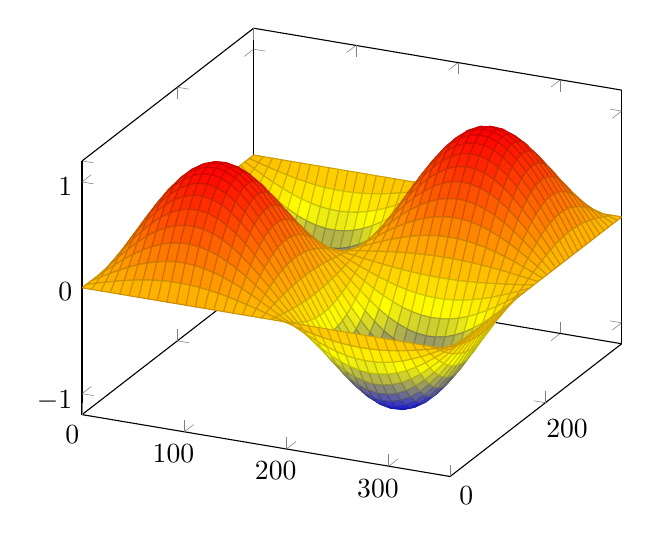
\begin{tikzpicture}
\begin{axis}
\addplot3[
surf,
domain=0:360,
samples=40,
] {sin(x)*sin(y)};
\end{axis}
\end{tikzpicture}
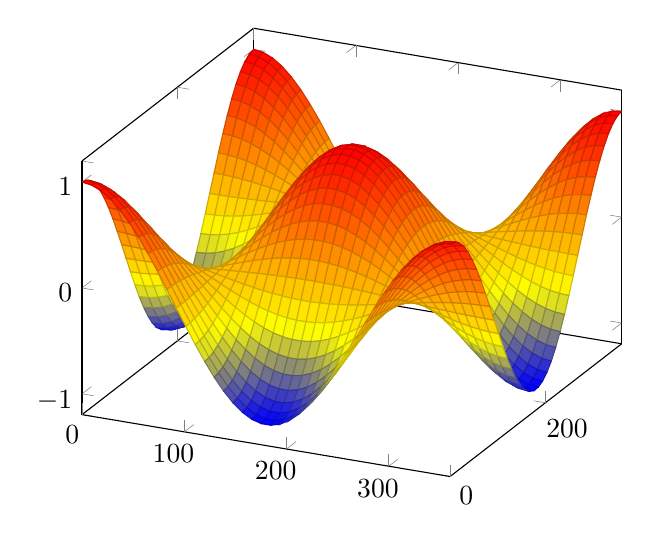
\begin{tikzpicture}
\begin{axis}
\addplot3[
surf,
domain=0:360,
samples=40,
] {cos(x)*cos(y)};
\end{axis}
\end{tikzpicture}

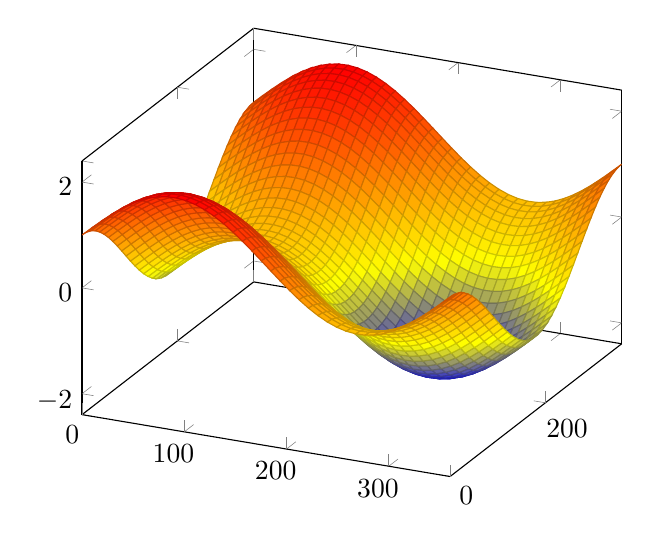
\begin{tikzpicture}
\begin{axis}
\addplot3[
surf,
domain=0:360,
samples=40,
] {sin(x)+cos(y)};
\end{axis}
\end{tikzpicture}
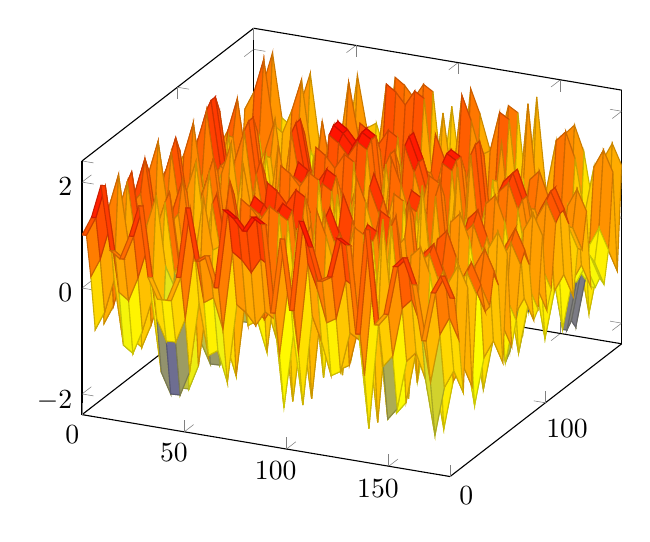
\begin{tikzpicture}
\begin{axis}
\addplot3[
surf,
domain=0:180,
samples=40,
] {sin(x*x)+cos(y*y)};
\end{axis}
\end{tikzpicture}

\begin{tikzpicture}
\begin{axis}
\addplot gnuplot [
id=sin,
] {sin(x)};
\end{axis}
\end{tikzpicture}


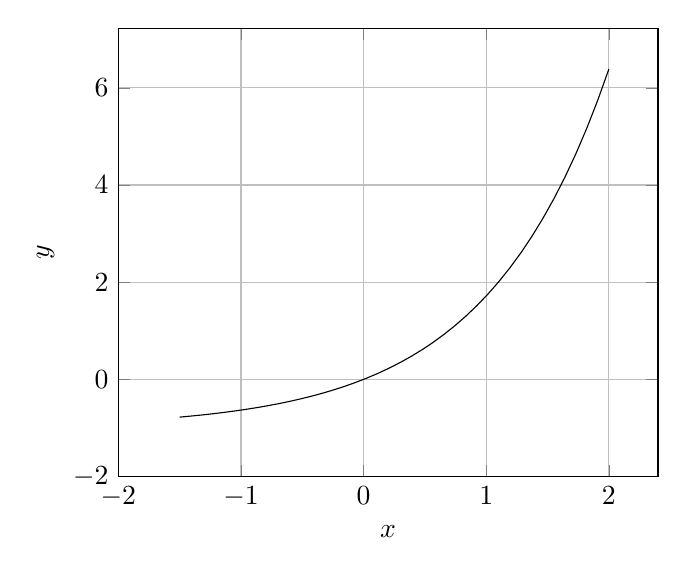
\begin{tikzpicture}
\begin{axis}[
xmin=-2,
ymin=-2,
xlabel= $x$,
ylabel= $y$,
grid=major,
]
\addplot[
domain=-1.5:2,
samples=40,
] {e^x-1};
\end{axis}
\end{tikzpicture}

\begin{tikzpicture}
\begin{axis}[
axis line=center,
xmin=-5.5,
ymin=-4,
xlabel= $x$,x label style={right},
ylabel= $y$,y label style= {above},
grid=major,
]
\addplot[
domain=-5.5:3,
samples=100,
] {1+x+x^2/2+x^3/6+x^4/24};
\end{axis}
\end{tikzpicture}


\begin{tikzpicture}
\datavisualization [school book axes, visualize as smooth line]
data [format=function] {
var x : interval [-1.3:1.3];
func y = \value x*\value x*\value x;
};
\end{tikzpicture}


\section{Symbols, Shortcuts and Semantic Aliasing}

Although Journals recommend not to alias LaTeX commands the harsh reality is that each topic and paper has different needs for notations and things can get messy.

Consider papers written for computations of floating algorithms. We might find in preambles definitions like, 
{\parskip0pt\large
\begin{verbatim}
%% Floating-point machine operations.
\newcommand{\mop}{\boxcircle}
\newcommand{\madd}{\boxplus}
\newcommand{\msub}{\boxminus}
\newcommand{\mmul}{\boxdot}
\newcommand{\mdiv}{\boxdiag}
\end{verbatim}
}
\newcommand{\mop}{\boxcircle}
\newcommand{\madd}{\boxplus}
\newcommand{\msub}{\boxminus}
\newcommand{\mmul}{\boxdot}
\newcommand{\mdiv}{\boxdiag}

I consider aliasing of non-semantic commands to semantic commands, such as the machine operation |\mop| from |\boxcircle| as good practice. 

\begin{texexample}{Example with macro aliasing}{ex;aliasing}
\begin{Definition} \summary{(Absorption.)}
Let $x, y, z \in \Fset$ with $y, z \in \Rset$,
let $\mathord{\mop}$ be any IEEE~754 floating-point operator,
and let $x = y \mop z$.
Then $y \mop z$ gives rise to \emph{absorption} if
\begin{itemize}
\item
$\mathord{\mop} = \mathord{\madd}$
and either $x = y$ and $z \neq 0$, or $x = z$ and $y \neq 0$;
\item
$\mathord{\mop} = \mathord{\msub}$
and either $x = y$ and $z \neq 0$, or $x = -z$ and $y \neq 0$;
\item
$\mathord{\mop} = \mathord{\mmul}$
and either $x = \pm y$ and $z \neq \pm 1$, or $x = \pm z$ and $y \neq \pm 1$;
\item
$\mathord{\mop} = \mathord{\mdiv}$,
$x = \pm y$ and $z \neq \pm 1$.
\end{itemize}
\end{Definition}
\end{texexample}


The most obvious shortcuts should be for calligraphic or fraktur math alphabets.


\begin{texexample}{Calligraphic Alphabet}{ex:callalphabet}
\providecommand*{\cA}{\ensuremath{\mathcal{A}}}
\providecommand*{\cB}{\ensuremath{\mathcal{B}}}
\providecommand*{\cC}{\ensuremath{\mathcal{C}}}
\providecommand*{\cD}{\ensuremath{\mathcal{D}}}
\providecommand*{\cE}{\ensuremath{\mathcal{E}}}
\providecommand*{\cF}{\ensuremath{\mathcal{F}}}
\providecommand*{\cG}{\ensuremath{\mathcal{G}}}
\providecommand*{\cH}{\ensuremath{\mathcal{H}}}
\providecommand*{\cI}{\ensuremath{\mathcal{I}}}
\providecommand*{\cJ}{\ensuremath{\mathcal{J}}}
\providecommand*{\cK}{\ensuremath{\mathcal{K}}}
\providecommand*{\cL}{\ensuremath{\mathcal{L}}}
\providecommand*{\cM}{\ensuremath{\mathcal{M}}}
\providecommand*{\cN}{\ensuremath{\mathcal{N}}}
\providecommand*{\cO}{\ensuremath{\mathcal{O}}}
\providecommand*{\cP}{\ensuremath{\mathcal{P}}}
\providecommand*{\cQ}{\ensuremath{\mathcal{Q}}}
\providecommand*{\cR}{\ensuremath{\mathcal{R}}}
\providecommand*{\cS}{\ensuremath{\mathcal{S}}}
\providecommand*{\cT}{\ensuremath{\mathcal{T}}}
\providecommand*{\cU}{\ensuremath{\mathcal{U}}}
\providecommand*{\cV}{\ensuremath{\mathcal{V}}}
\providecommand*{\cW}{\ensuremath{\mathcal{W}}}
\providecommand*{\cX}{\ensuremath{\mathcal{X}}}
\providecommand*{\cY}{\ensuremath{\mathcal{Y}}}
\providecommand*{\cZ}{\ensuremath{\mathcal{Z}}}
\begin{luacode}
local alphabet = {"A","B","C","D","E","F","G","H","I","J","K","L",
                  "M","N","O","P","Q","R","S","T","U",
                  "V","W","X","Y","Z"}
for k,v in pairs(alphabet) do
	tex.print("\\c"..v..", ")
end
\end{luacode}
\end{texexample}


\section{Calculus}



\subsection*{Differentiation}
Leibnitz invented the transmutation theorem for finding the area under a curve. Finding areas beneath curves
was 


\subsection*{Integration}

\subsection*{Limits}

\marginpar{\includegraphics[width=3cm]{bolzano}
{\scriptsize\RaggedLeft Bolzano begins his work by explaining what he means by theory of science, and the relation between our knowledge, truths and sciences. Human knowledge, he states, is made of all truths (or true propositions) that men know or have known. This is, however, only a very small fraction of all the truths that exist, although still too much for one human being to comprehend. Therefore, our knowledge is divided into more accessible parts. Such a collection of truths is what Bolzano calls a science (Wissenschaft). It is important to note that not all true propositions of a science have to be known to men; hence, this is how we can make discoveries in a science.}}

\textbf{Bolzano} Although implicit in the development of calculus of the 17th and 18th centuries, the modern idea of the limit of a function goes back to Bolzano who, in 1817, introduced the basics of the epsilon-delta technique to define continuous functions. However, his work was not known during his lifetime.\footcite{coolidge} The first publication in English had to wait for almost 150 years and it was published by Coolidge in 1949 in his popular work \emph{The Mathematetics of Great Amateurs.} Grattan-Guiness\footcite{grattan-guiness} falls short though of accusing Cauchy of plagiarizing the work of Bolzano and other contemporaries.


\textbf{Cauchy} discussed variable quantities, infinitesimals, and limits and defined continuity of {$\displaystyle y=f(x)$} $y=f(x)$ by saying that an infinitesimal change in $x$ necessarily produces an infinitesimal change in $y$ in his 1821 book \emph{Cours d'analyse}, while (Grabiner 1983) claims that he only gave a verbal definition. 

\textbf{Weierstrass} first introduced the epsilon-delta definition of limit in the form it is usually written today. He also introduced the notations $\lim$ and $\lim x\rightarrow x_0$. The notation which has been used widely at the time in Europe was
$\operatorname{Lim}_{x=a}$, to express the \enquote{the limit as $x$ approaches $a$.} It is found in papers of Weierstrass, who in 1841 wrote $\lim$ and in 1854 \enquote{$\underset{n=\infty}{\operatorname{Lim.}}\:p_n = \infty $}

In later publications we find $\operatorname{Lim}$ without the point, but still capitalized. I particularly like the way the equations were grouped and the limit indicated by cases and shown in fig.~\ref{weis}.

\begin{figure}[htbp]
\centering
\includegraphics[width=0.8\textwidth]{weistrass}
\caption{Extract from Weierstrass publication.}
\label{weis}

\end{figure}

To create a new operator symbol we can use \cs{operatorname}. The command will take care of spacing, whereas if we use only
|\mathrm| it will not. If we were to use it frequently we could also define a macro using \cs{DeclareMathOperator} from amsmath. 

\begin{texexample}{operatorname}{ex:onames}

$$\operatorname{Lim.}p_n$$

$$\operatorname{Lim}.p_n$$

$$\mathrm{Lim.}p_n$$ 
\end{texexample}

By the early 1900's the notation started approaching more to what is commonly used in today's publications.

\textbf{Hardy} The modern notation of placing the arrow below the limit symbol is due to Hardy in his book \emph{A Course of Pure Mathematics} in 1908, however in the preface to the book he credits Leathem and Bromwich\footcite{bromwich}.\footnote{Hardy wrote ... there are two respects in which I have diverted ...} 


\begin{gather}
\begin{aligned}
f(a) &= f\left[\lim_{k\rightarrow\infty} x_k \right]=\lim_{k} f(x_k)\le 0 & \text{ and }\\
f(a) &= f\left[\lim_{k\rightarrow\infty} X_k \right]=\lim_{k} f(X_k)\ge 0. & \\  
\end{aligned}
\end{gather}

In Cauchy's words, these inequalities established that ``the quantity
$f(a)$ \ldots cannot differ from zero.'' He had thus proved the existence of a
number a between $x$ and $X$ for which $f(a) = O$. The general version of the
intermediate value theorem, namely that a continuous function takes all
values between $f(x_0)$ and $f(X)$, follows as an easy corollary.
This was a remarkable achievement. Cauchy had, for the most part,
succeeded in demonstrating a "self-evident" principle by analytic methods.


Apart from open intervals, limits can be defined for functions on arbitrary subsets of R, as follows.  Let $f$ be a real-valued function defined on a subset $S$ of the real line.  Let $p$ be a limit point of ''S'' that is, ''p'' is the limit of some sequence of elements of ''S'' distinct from p.  The limit of ''f'', as ''x'' approaches ''p'' from values in ''S'', is ''L'' if, for every {{nowrap|''ε'' > ''0''}}, there exists a δ > ''0'' such that {{nowrap|0 < {{abs|''x'' − ''p''}} < ''δ''}} and {{nowrap|''x'' ∈ ''S''}} implies {{nowrap|{{abs|''f''(''x'') − ''L''}} < $\epsilon$.

This limit is often written

\[
L = \underset{x\in S}{\lim_{x\to p}} f(x).
\]

The condition that $f$ be defined on $S$ is that $S$ be a subset of the domain of $f$.  This generalization includes as special cases limits on an interval, as well as left-handed limits of real-valued functions (e.g., by taking ''S'' to be an open interval of the form $(-\infty,a)$, and right-handed limits (e.g., by taking ''S'' to be an open interval of the form $(a,\infty)$. It also extends the notion of one-sided limits to the included endpoints of (half-)closed intervals, so the Square root function $f(x)=\sqrt{x}$ can have limit 0 as $x$ approaches 0 from above.




\section*{Fraktur letters}

Individual Fraktur letters are sometimes used in mathematics, which often denotes associated or parallel concepts by the same letter in different fonts. For example, a Lie group is often denoted by ''G'', while its associated Lie algebra is $\mathfrak{g}$. 
A ring ideal might be denoted by $\mathfrak{a}$ (or $\mathfrak{p}$ if a prime ideal) while an element is $a \in \mathfrak{a}$. The Fraktur $\mathfrak c$ is also sometimes used to denote the cardinality of the continuum, that is, the cardinality of the real line. In model theory, $\mathfrak{A}$ is used to denote an arbitrary model, with ''A'' as its universe. Fraktur is also used in other ways at the discretion of the author.


\begin{luacode}
local alphabet = {"A","B","C","D","E","F","G","H","I","J","K","L",
                  "M","N","O","P","Q","R","S","T","U","V","W","X","Y","Z"}
for k,v in pairs(alphabet) do
	tex.print("\\mathfrak{"..v.."}, ")
end
\end{luacode}

Special symbols such as dingbats loaded using the \pkg{pifont} package need to be enclosed within an \docAuxCommand{mbox} in order to be able to display the glyph properly.
\bigskip

\begin{texexample}{Using special dingbat symbols}{}
\label{e14}
 We start by showing that the function $f(x)=x^2$ is
continuous over the set $X_2$\label{p:X2} defined as the interval
$[0,1]$ where numerals $\frac{i}{\mbox{\ding{172}}}, 0 \le i \le
\mbox{\ding{172}},$ are used to express its points in units $\mu$.
First of all, note that the set $X_2$ is continuous in   $\mu$
because its points are equidistant with the distance
$d=\mbox{\ding{172}}^{-1}$. Since this function is strictly
increasing,  to show its continuity it is sufficient to check the
difference $f(x)-f(x^{-})$ at the point $x=1$. In this case,
$x^{-}=1-\mbox{\ding{172}}^{-1}$ and we have
\[
 f(1)-f(1-\mbox{\ding{172}}^{-1})=
 1-(1-\mbox{\ding{172}}^{-1})^2 =
 2\mbox{\ding{172}}^{-1}(-1)\mbox{\ding{172}}^{-2}.
\]
This number is infinitesimal, thus $f(x)=x^2$ is continuous over
the set $X_2$. \hfill $\Box$
\end{texexample}

\cs{Box}
Notice the use of the \docAuxCommand{Box} command to draw a square for  end of proof symbol. This is from the amsmath package. The box is placed at the end of the line using |\hfill $\Box$|.

%
%\begin{Rule}
%Alias common symbols to semantic macro names that follow their mathematical definitions.
%\end{Rule}
%
%\begin{Rule}
%Create shorcut commands with moderation for alphabets and algebras and alias if necessary. Good practice, sets etc.
%\end{Rule}



\section{Partial derivatives}

Partial derivatives can be typeset using the \latex{} command \cs{partial}

\begin{texexample}{Partial Derivatives}{ex:partial}
\[
dS = \frac{\partial S}{\partial x}\, dx
   + \frac{\partial S}{\partial y}\, dy
   = \left(y - \frac{2V}{x^2}\right) dx
   + \left(x - \frac{2V}{y^2}\right) dy.
\]
\meaning\partial
\end{texexample}


This is using a certain style. For other styles it maybe more difficult.

\section*{Binomial Coefficients}

To typeset binomial coefficients or similar structures, use the command
\cs{binom} from \pkg{amsmath}\index{amsmath>binom}

\begin{texexample}{Binomial}{ex:binomial0}
\[
\begin{align}
(x+y)^3 & = x^3 + 3x^2y + 3xy^2 + y^3, \\[8pt]
(x+y)^4 & = x^4 + 4x^3y + 6x^2y^2 + 4xy^3 + y^4, \\[8pt]
(x+y)^5 & = x^5 + 5x^4y + 10x^3y^2 + 10x^2y^3 + 5xy^4 + y^5, \\[8pt]
(x+y)^6 & = x^6 + 6x^5y + 15x^4y^2 + 20x^3y^3 + 15x^2y^4 + 6xy^5 + y^6, \\[8pt]
(x+y)^7 & = x^7 + 7x^6y + 21x^5y^2 + 35x^4y^3 + 35x^3y^4 + 21x^2y^5 + 7xy^6 + y^7.
\end{align}
\]
\end{texexample}


Pascal's rule can be typeset as:


\begin{texexample}{Binomial Distribution}{ex:binomial}
\[
\binom{n}{k} =\binom{n-1}{k}
+ \binom{n-1}{k-1}
\]
\end{texexample}



\section[Symbols and Abbreviations]{Symbols and Abreviations}
\label{math:abbreviations}

\label{abbr}\label{symbols}%

\begin{texexample}{Creating symbols}{ex:parallelogram}
\newlength{\dentwidth}\setlength{\dentwidth}{\textwidth}
\addtolength{\dentwidth}{-\parindent}

\makeatletter
\gdef\@parallelogram#1{%
  \textnormal{\setbox\z@\hbox{#1/}\dimen@\wd\z@
   \@tempdima 2.45\dimen@
   \vbox{\offinterlineskip
      \hbox{\kern.8\dimen@\vrule\@width\@tempdima\@height.4\p@}%
      \kern-.0\p@
      \hbox to\@tempdima{#1/\hfil\rlap/}%
      \kern-.5\p@
      \hbox{\kern.1\dimen@\vrule\@width\@tempdima\@height.4\p@}}}}
      
 \gdef\Par{%
   \mathchoice
      {\@parallelogram\scriptsize}%
      {\@parallelogram\scriptsize}%
      {\@parallelogram\tiny}%
      {\@parallelogram\tiny}}

            



\begin{tabular*}{\dentwidth}{rl@{\extracolsep{\fill}}l@{\extracolsep{0pt}}@{\dots}l}

$>$ & is (or are) greater than. & Def. & definition. \\
$<$ & is (or are) less than. & Ax. & axiom. \\
$\Bumpeq$ & is (or are) equivalent to. & Hyp. & hypothesis. \\
$\therefore$ & therefore. & Cor. & corollary. \\
$\perp$ & perpendicular. & Scho. & scholium. \\
$\perp_s$ & perpendiculars. & Ex. & exercise. \\
$\parallel$ & parallel.\qquad $\parallel_s$ parallels. & Adj. & adjacent. \\
$\angle$ & angle.\qquad $\angle_s$ angles. & Iden. & identical. \\
$\triangle$ & triangle.\qquad $\triangle_s$ triangles. & Const. & construction. \\
$\Par$ & parallelogram. & Sup. & supplementary. \\
$\Par_s$ & parallelograms. & Ext. & exterior. \\
$\odot$ & circle.\qquad $\odot_s$ circles. & Int. & interior. \\
rt. & right.\qquad  st.\ straight. & Alt. & alternate. \\
\end{tabular*}


\hbox{\qed\ stands for quod erat demonstrandum, \emph{which was to be proved}.\hss}

\newcommand{\qef}{\textsc{q.e.f.}}
\qef\ stands for quod erat faciendum, \emph{which was to be done.}

The signs $+$, $-$, $\times$, $\div$, $=$, have the same meaning as in Algebra.

\makeatother   
\end{texexample}
   
\section{Afixing symbols to other symbols}

\latex provides \docAuxCommand{stackrel} for placing a superscript above a binary relation. In the \pkg{amsmath} package there are somewhat more general commands \docAuxCommand{overset} and \docAuxCommand{underset}, that can be used to place one symbol above or below another symbol, whether is a relation or something else. Oberdiek's package \pkg{stackrel}\footcite{stackrel} extends the syntax by adding an optional argument for the subscript position. It follows the syntax of extensible arrows of the packages |amsmath| and |mathtools|.

\begin{docCommand}{stackrel}{\oarg{subscript}\marg{superscript}{\marg{rel}}}
  Typeset a subscript or superscript above a symbol.
\end{docCommand}

\ifSTACKREL
\begin{texexample}{Example of stackrel and stackbin}{ex:stackrel}
\[
 A \stackbin[\text{and}]{}{+} B \stackrel[x]{!}{=} C
\] 
\end{texexample}
\else
\begin{texcode}{Example of \cs{stackrel} and \cs{stackbin}}{ex:stackrel}
  Example cannot be shown as the package stackrel is not loaded.
\end{texcode}
\fi


\chapter{Matrices and Mathematical Environments}
\label{matrices}

\section{Matrices}

Matrices have a long history of application in solving linear equations but they were known as arrays until the 1800s. The Chinese text The Nine Chapters on the Mathematical Art written in 10th–2nd century BCE is the first example of the use of array methods to solve simultaneous equations,[102] including the concept of determinants. In 1545 Italian mathematician Gerolamo Cardano brought the method to Europe when he published Ars Magna.[103] The Japanese mathematician Seki used the same array methods to solve simultaneous equations in 1683.[104] 


The Dutch statesman and mathematician Johan (Jan) de Witt represented transformations resembling arrays in his 1659 book Elements of Curves (1659). He is also perhaps the second Mathematician to be lynched\footnote{Hypatia, was torn to bits by a lynching Christian mob in the streets of Alexandria in \textsc{AD} 415.} by a mob and had parts of their bodies eaten! [\ldots]The brothers were shot and then left to the mob. Their naked, mutilated bodies were strung up on the nearby public gibbet, while the Orangist mob partook of their roasted livers in a cannibalistic frenzy. Throughout it all, a remarkable discipline was maintained by the mob, according to contemporary observers, making one doubt the spontaneity of the event.\footcite{israel1995} \textit{Elementa Curvarum Linearum} has been described as the first textbook in analytic geometry.\footnote{The savage murder of a man that history has judged a highly competent leader is regarded by the Dutch as one of the most shameful episodes in their history.}


Between 1700 and 1710 Gottfried Wilhelm Leibniz publicized the use of arrays for recording information or solutions and experimented with over 50 different systems of arrays.[103] Cramer presented his rule in 1750.

The term "matrix" (Latin for "womb", derived from mater—mother[106]) was coined by James Joseph Sylvester in 1850,[107] who understood a matrix as an object giving rise to a number of determinants today called minors, that is to say, determinants of smaller matrices that derive from the original one by removing columns and rows. In an 1851 paper, Sylvester explains:

\begin{quote}
I have in previous papers defined a \enquote{Matrix} as a rectangular array of terms, out of which different systems of determinants may be engendered as from the womb of a common parent.[108]
\end{quote}

Arthur Cayley published a treatise on geometric transformations using matrices that were not rotated versions of the coefficients being investigated as had previously been done. Instead he defined operations such as addition, subtraction, multiplication, and division as transformations of those matrices and showed the associative and distributive properties held true. Cayley investigated and demonstrated the non-commutative property of matrix multiplication as well as the commutative property of matrix addition.[103] Early matrix theory had limited the use of arrays almost exclusively to determinants and Arthur Cayley's abstract matrix operations were revolutionary. He was instrumental in proposing a matrix concept independent of equation systems. In 1858 Cayley published his A memoir on the theory of matrices[109][110] in which he proposed and demonstrated the Cayley–Hamilton theorem.[103] Cayley introduced a particular notation for fencing the array as shown in fig~\ref{fig:cayley}, which used () for the first row and $\vert$ for subsequent rows.

\begin{figure}[htbp]
\centering
\includegraphics[width=0.6\textwidth]{cayley-notation}

\caption{Extract from Caley's paper \textit{A memoir on the theory of matrices.}}
\label{fig:cayley}

\end{figure}

An English mathematician named Cullis was the first to use modern bracket notation for matrices in 1913 and he simultaneously demonstrated the first significant use of the notation $A = [a_{i,j}]$ to represent a matrix where $a_{i,j}$ refers to the i$^$th row and the $j$th column.

Cayley's introductory paper in matrix theory was written in French and published in a German periodical. In this paper, matrices are introduced to simplify the notation which arises in simultaneous linear equations.  

\begin{gather}
\begin{aligned}
\xi  &= \alpha x + \beta y + \gamma z + \dots\\
\eta  &= \alpha' x + \beta' y + \gamma' z + \dots\\
\zeta &= \alpha'' x + \beta'' y + \gamma'' z + \dots
\end{aligned}
\end{gather}

The set of equations is written as:

\begin{gather}
(\xi, \eta, \zeta,\dots ) = (\alpha,\beta,\gamma,\dots)(x,y,z,\dots)
\end{gather}

The same article also introduces, although quite sketchily, the ideas of inverse matrix and of matrix multiplication, or \enquote{compounding} as Cayley called it. The above basic properties are expanded in a second expository article\footcite{fieldman1962} which
also lists many additional properties of matrices. In this important paper, Cayley works mostly with square matrices with
nine elements. He represents the zero matrix,\footcite[This is an interesting development]{fieldman1962}

\[
\begin{vmatrix}
0,0,0\\
0,0,0\\
0,0,0
\end{vmatrix}
\]
by \enquote{0} and the \enquote{matrix unity,}

\[
\begin{vmatrix}
1,0,0\\
0,1,0\\
0,0,1
\end{vmatrix}
\]
by \enquote{1}

Caley then introduces the algebra of matrices by defining the addition of two matrices by

\begin{gather}
(\begin{cayleymatrix}{3}
a&b&c\\
a' &b' & c'\\
a''&b'' & c''\\
a''' & b''' & c'''\\
\end{cayleymatrix}) +
(\begin{cayleymatrix}{3}
\alpha & \beta & \gamma\\
\alpha & \beta & \gamma\\
\alpha & \beta & \gamma\\
\end{cayleymatrix})\:\: = \:\:
(\begin{cayleymatrix}{3}
a+a  &b+b  &c+\gamma\\
a''+\alpha' & b'' + \beta'' & c'' +\gamma'' \\
a'''+\alpha''' & b''' + \beta''' & c''' +\gamma''' \\
\end{cayleymatrix})
\end{gather}
Caley stated but without proof, that matrices are commutative and associative under addition. Two types
of multiplication are exhibited. The first type is designated as \enquote{scalar multiplication,} that is

\[
m(\begin{cayleymatrix}{3}
a & b & c\\
a' & b' & c'\\
a'' & b'' & c''
\end{cayleymatrix}) 
= 
(\begin{cayleymatrix}{3}
ma & mb & mc\\
ma' & mb' & mc'\\
ma'' & mb'' & mc''
\end{cayleymatrix})
\]

The notation used for the matrix (\begin{cayleymatrix}{3}
a&b\\
c&d\\
e&f
\end{cayleymatrix}) is defined later on. It is a special environment.

The second type of multiplication is called \enquote{compounding,} according to the following scheme:

\begin{multline}
(\begin{cayleymatrix}{3}
a  &b &c\\
a' &b' &c'\\
a'' &b'' &c''
\end{cayleymatrix}\between \begin{cayleymatrix}{3}
\alpha & \beta & \gamma\\
\alpha'' & \beta'' & \gamma''\\
\alpha'' & \beta'' & \gamma''\\
\end{cayleymatrix})
\\=
 (\begin{cayleymatrix}{3} \bigl(a,b,c\between a, a',a''\bigr) & (a,b,c\between (\beta, \beta', \beta'') & (a,b,c\between \gamma, \gamma', \gamma'')\\
(a &b &c\\
(a &b &c
\end{cayleymatrix})\label{caleyprod}
\end{multline}

The product equation is complex to type, but very clear to understand its definition.\footnote{Uses multline environment.}


Later developments are described by Feldmann\footcite[This is the second paper that appeared in the \textit{The Mathematics Teacher relating to matrices.}][]{feldmann1963}. 

In the 1930s books on matrices written in English started to appear. The two leading ones were C.C. MacDuffee \textit{Theory of Matrices,} Springer (1933) and J. H. M. Wedderburn \textit{Lectures on Matrices}\footnote{The book was published by the American Mathematical Society and bears reseblance to a publication printed using TeX.} (1934). They both wrote matrices with double vertical lines as in

\[
\begin{Vmatrix}
a_{11} & a_{12} & \dots & a_{1n}\\
a_{11} & a_{12} & \dots & a_{1n}\\
\vdots & \vdots & \vdots & \vdots\\
a_{n1} & a_{n2} & \dots &a_{nn}
\end{Vmatrix}
\]
The use of double vertical lines was easy to typeset as well as to handwrite. It could also relate to the single vertical lines which are used to denote determinants.




%%%%%%%%%%%%%%%%%%%%%%%%%%%%%%%%%%%%%%%%%%%%%
%%%%%%%%  TYPOGRAPHY %%%%%%%%%%%%%%%%%%%%%%%%
\section{Typography of Matrices}

Matrices are mostly typed the way tabular environements are types, i.e., you need to use the tabulator sign ``\&''.
Mathematical environments are provided both by \latexe as well as amsmath. The latter are to be preferred.

\begin{docEnvironment}{array}{\marg{specifier}}
\end{docEnvironment}

The |array| environment is a \latex2e provided environment and is identical to tabular, but works automatically with mathematics. It has to be enclosed in a mathematical environment.


\begin{texexample}{Matrices}{ex:matrices}
\[
\mathbf{X} = \left(
\begin{array}{ccc}
x_1 & x_2 & \ldots \\
x_3 & x_4 & \ldots \\
\vdots & \vdots & \ddots
\end{array} \right)
\]
\end{texexample}

\section{AMS Math matrices}

The \pkg{amsmath} package provides environments that go beyond the basic \docAuxEnvironment{array} of \latex2e. The \docAuxEnvironment{pmatrix}, \docAuxEnvironment{Bmatrix}, \docAuxEnvironment{vmatrix} and \docAuxEnvironment{Vmatrix}. 
There is also a \docAuxEnvironment{smallmatrix} that is more suitable for inline text display. 

\begin{texexample}{Using \textbackslash smallmatrix}{ex:smallmatrix}
This is a small matrix $\bigl(\begin{smallmatrix}
a&b\\
c&d\\
\end{smallmatrix}\bigr)$ environment. \lorem
\end{texexample}


\begin{docEnvironment}{bmatrix}{}
The example \ref{ex:bmatrix} illustrates the typesetting of a bracketted matrix hence \ul{b}matrix. If you want the matrix equation to be numbered enclose it withn an |equation| or |gather| environment. In this documentation we have let the |equation| environment to |gather| hence it will make no difference which ever is used. (amsmath)
\end{docEnvironment}

\begin{texexample}{Bmatrix}{ex:bmatrix}
\begin{equation}
\begin{matrix}
1 & 2 \\
3 & 4
\end{matrix} \qquad
\begin{bmatrix}
p_{11} & p_{12} & \ldots & p_{1n} \\
p_{21} & p_{22} & \ldots & p_{2n} \\
\vdots & \vdots & \ddots & \vdots \\
p_{m1} & p_{m2} & \ldots & p_{mn}
\end{bmatrix}
\end{equation}
\end{texexample}

The \refEnv{bmatrix} is from the amsmath package, see also \vref{bmatrix} and \nameref{bmatrix} and \pageref{bmatrix}. 


One issue to be aware is that the \refEnv{bmatrix} does not allow more than 10 tab stops. If you need to use more, you will have to \docCounter{MaxMatrixCols} to a higher number. The |phd| package sets this automatically at 20, so you will not have to worry about it.

\begin{teX}
\setcounter{MaxMatrixCols}{20}
\end{teX}

\begin{texexample}{Large Matrices}{ex:largematrices}
\[
\begin{bmatrix}
1 & 0 & 0 & -1 & 0  & 0  & 1 & -1 & 1  & -1 & 0 \\
0 & 1 & 0 & 0  & -1 & 0  & 1 & -1 & 0  & 1  & -1 \\
0 & 0 & 1 & 0  & 0  & -1 & 1 & -1 & -1 & 0  & 1 
\end{bmatrix}
\]
\end{texexample}



\section{vmatrix}

\begin{texexample}{vmatrix}{ex:vmatrix}

\begin{gather}
\begin{vmatrix}
aa' + bb' + cc' & ea' + fb' + gc' \\
ae' + bf' + cg' & ee' + ff' + gg'
\end{vmatrix}
{} = \begin{vmatrix}
a & b \\
e & f
\end{vmatrix}  \begin{vmatrix}
a' & b' \\
e' & f'
\end{vmatrix} + \begin{vmatrix}
a & c \\
e & g
\end{vmatrix}  \begin{vmatrix}
a' & c' \\
e' & g'
\end{vmatrix}.
\end{gather}
\end{texexample}





\section{Single equations that are too long}

In many cases equations need to be written over two or more lines. The \pkgname{amsmath} package, provides environments that are suitable for this:


\begin{texexample}{The multiline amsmath environment}{ex:multiline}
\begin{multline}
   a + b + c + d + e + f+ g + h + i  + k + l + m + n + o + p\\
              = j + k + l + m + n +\cos^{2}-1
\end{multline}
\end{texexample}



\section{array environment}

This is simply the same as the |eqnarray| environment only with the possibility of
variable rows and columns and the fact, that the whole formula has only one
equation number and that the array environment can only be part of another math
environment, like the equation environment or the displaymath environment. With
@{} before the first and after the last column the additional space |\arraycolsep| is
not used, which maybe important when using left aligned equations.

\begin{texexample}{array environment}{ex:array2}
\begin{eqnarray}
  a & = & b + c \\
    & = & d + e + f + g + h + i
               + j + k + l \nonumber \\
    &   & +\: m + n + o \\
    & = & p + q + r + s
\end{eqnarray}
\end{texexample}

The equations
to be aligned are entered with each one terminated by \cs{cr}. In each equation there should be
one alignment symbol \& to indicate where the alignment should take place. This is usually
done at the equal signs, although it is not necessary to do so. For example


\begin{texexample}{The array environment}{ex:array}
Thus to change $\frac34$ to a decimal divide $4$ into $3$
and we get $.75$ as a result, thus:
\[
\begin{array}{r@{}r@{}}
4 \; & \vline \; 3.00 \\\cline{2-2}
     &            .75
\end{array}
\]

To find the square root of a four-figure number
such as our example calls for, work it out in the
following manner:
\[
\arraycolsep=0em
\begin{array}{cccccccccccc}
\multicolumn{3}{c}{\text{2d pair}} &\qquad&\qquad&
\multicolumn{3}{c}{\text{1st pair}}&\qquad&\qquad&
\multicolumn{2}{c}{\text{square root}}\\
 & \overbrace{\quad}&\ZZZ&&&\ZZZ&\overbrace{\quad}&\ZZZ\\
 & 42 &&&&& 25 &&&&\vline\;65&(answer)\\\cline{11-11}
 & 36 &&&&& \\\cline{2-2}
\multirow{2}{*}{125\:} & \vline\hfill \Zi6 \hfill&&&&& 25\\
 & \vline\hfill \Zi6 \hfill&&&&& 25\\\cline{2-7}
\end{array}
\]
\end{texexample}


\subsection{Array environment in game theory}

This example \ref{ex:gamearray} is from \footnote{From determinacy to Nash equilibrium,St\'ephane Le Roux, TU Darmstadt }

\begin{texexample}{array environment in game theory}{ex:gamearray}
The game $\langle\{a,b,c\},\{1,2,3,4\}^3,\{0,1,2,3,4\},v,(<_d)_{d\in\{a,b,c\}}
\rangle$ is represented below, where player $a$ chooses the row, $b$ the column, and $c$ the array. 
\[\begin{array}{c@{\hspace{1cm}}c@{\hspace{1cm}}c@{\hspace{1cm}}c}
\begin{array}{|c|c|c|c|}
\hline 1 & 1 & 1 & 1\\
\hline 1 & 1 & 1 & 1\\
\hline 1 & 1 & 1 & 1\\
\hline 4 & 1 & 1 & 1\\
\hline
\end{array}
&
\begin{array}{|c|c|c|c|}
\hline 1 & 2 & 1 & 1\\
\hline 2 & 2 & 2 & 2\\
\hline 1 & 2 & 1 & 1\\
\hline 4 & 2 & 1 & 1\\
\hline
\end{array}
&
\begin{array}{|c|c|c|c|}
\hline 1 & 1 & 3 & 1\\
\hline 1 & 1 & 3 & 1\\
\hline 3 & 3 & 3 & 3\\
\hline 4 & 1 & 3 & 1\\
\hline
\end{array}
&
\begin{array}{|c|c|c|c|}
\hline 2 & 4 & 4 & 4\\
\hline 4 & 3 & 4 & 4\\
\hline 4 & 4 & 4 & 4\\
\hline 0 & 0 & 0 & 0\\
\hline
\end{array}
\end{array}
\]
Let us show that the game $\langle\{a,b,c\},\{1,\dots,n\}^3,\{0,\dots,n\},v,(<_d)_{d\in\{a,b,c\}}
\rangle$ witnesses the claim. First, the preferences are linear orders indeed. Second, let us show that there is no Nash equilibrium by case-splitting below. 
\end{texexample}



\section{The AMSmath Package}

\index{maths environment>align}
\index{maths environment>align}
\index{maths environments}{falign}
\index{maths environments}{xalignat}
\index{maths environments}{xxalignat}
\index{maths environments}{eqnarray}

The \pkg{amsmath} package offers five different align environments, |align|, |alignat|, |falign|, |xalignat| and |xxalignat|. 

In difference to the \refEnv{eqnarray} environment from standard \latex the ``three'' parts of one equation expr.-symbol-expr. are divided by only one ampersand in two parts. In general the ampersand should be before the symbol to get the right spacing, for example y \&= x. 

\subsection{The align environment}

The |align| environment is considered an improvement over \latex's |eqnarray| environment. It is very similar to a tabular
environment and is aligned at the |&|. 
It requires one |&| less and produces a tighter equation. Mathematicians 
are very particular in not using |eqnarray| and the package 
\pkgname{onlyamsomath} if used will warn if it finds that it has been used in the document. 
\index{eqnarray (environment)>spacing}
\index{eqnarray (environment)>alternatives}
\index{math environments>align}
\index{math environmenta>eqnarray}


\begin{texexample}{Comparison between |align| and |eqnarray|}{ex:eqnarraycomp}
% First example with eqnarray
\begin{eqnarray}
a & = & b + c \\
  & = & d + e + f + g + h + i
        + j + k + l \nonumber \\
  &   & +\: m + n + o \\
  & = & p + q + r + s
\end{eqnarray}

% Second example with align
\begin{align}
a & =  b + c \\
  & =  d + e + f + g + h + i
       + j + k + l \nonumber \\
  & +\: m + n + o \\
  & =  p + q + r + s
\end{align}
\end{texexample}


You can observe in Example~\ref{eqnarraycomp} the essential differences between the two, which we re-iterate, it requires one less |&| and produces a tighter display.

\begin{texexample}{The align environment}{ex:align}
\begin{align}
         y & = d\label{eq:IntoSection}\\
         y & = cx+d\\
    y_{12} & = bx^{2}+cx+d\\
     y(x)  & = ax^{3}+bx^{2}+cx+d
 \end{align}

%\begin{align*}
%\therefore (13 - x_1) + (13 - x_2) + \dotsb + (13 - x_p) + r &= 52\,,\\
%\therefore 13p - (x_1 + x_2 + \dotsb + x_p) + r              &= 52\,,\\
%\therefore x_1 + x_2 + \dotsb + x_p                          &= 13p - 52 + r\\
%                                                          &= 13 (p - 4) + r\,.
%\end{align*}

whence we conclude that $\gamma$ is a primitive root modulo $p$. But
\begin{align*}
\gamma^{p-1}-1 &=
     g^{p-1} - 1 + \frac{p-1}{1!}g^{p-2}xp +
        \frac{(p-1)(p-2)}{2!}g^{p-3}x^2p^2 + \ldots \\
  &= p\left(kp + \frac{p-1}{1!}g^{p-2}x +
        \frac{(p-1)(p-2)}{2!}g^{p-3}x^2p + \ldots\right).
\end{align*}
\end{texexample}

As you can observe from example\ref{ex:align}, each line is numbered if the unstarred version of the command is used. The |aligned| environment remedies this.
 


\subsection{The aligned environment}

The aligned environment allows more than one horizontal alignment but has only one equation number.

%\newcommand{\dotsbsmall}{\ldot\!\ldot\!\ldot}
%\newcommand{\ldot}{\mathbin{.}}			% dot with math spacing
%\newcommand{\nobf}[1]{\no \textbf{#1}}		% no with bold number
%
%\begin{texexample}{aligned environment example}{}
%\begin{equation}
%\begin{aligned}
%  &\:C_1x^{r_1}\,[\varphi_{r_1 0} \,+ \varphi_{r_1 1}\log x \,+ \dotsb + \varphi_{r_1 \alpha_1}(\log x)^{\alpha_1}]\\
%+ &\:C_2x^{r_2}\,[\varphi_{r_2 0} \,+ \varphi_{r_2 1}\log x \,+ \dotsb + \varphi_{r_2 \alpha_2}(\log x)^{\alpha_2}]\\
%+ &\multispan{1}{\:\dotfill}\\
%+ &\:C_nx^{r_n}[\varphi_{r_n 0} + \varphi_{r_n 1}\log x + \dotsb + \varphi_{r_n \alpha_n}(\log x)^{\alpha_n}],
%\end{aligned}
%\end{equation}
%
%\[
%\tag{98}
%\left\{\qquad
%\begin{aligned}
%T_1 &= T_2 = T_3 (=T)\\
%p_1 &= p_2 = p_3\\
%s_1-s_2 &= \frac{(u_1-u_2)+p_1(v_1-v_2)}{T}\\
%s_2-s_3 &= \frac{(u_2-u_3)+p_2(v_2-v_3)}{T}.
%\end{aligned}
%\right.
%\]
%\end{texexample}
 




\subsection{How to interrupt a display}

\begin{docCommand}{intertext}{}
 In many instances you will want to interrupt a display with some text. This can be accomplished using the control sequence |\intertext|.
 \end{docCommand}
 
 

\begin{texexample}{Using \cs{intertext}}{ex:intertext}
\begin{gather}
\begin{aligned}
U &= M u = M(c_v T + b)\\
S &= M(c_v  \log T + \frac{R}{m}  \log v + a),\\
\intertext{and } 
F &= M \left\{T(c_v - a - c_v \log T) - \frac{RT}{m} \log v + b \right\}.
\end{aligned}
\end{gather}
\end{texexample}

As the command \docAuxCommand{intertext} can only come after a |\\|  command we place it accordingly at {1}. Its function is to preserve the alignment after the text is typeset. This is a common requirement in many mathematical 
structures and the command can be used in all of amsmath aligning environments.







\subsection{The alignat environment}

\begin{docEnvironment}{alignat}{}
The alignat environment means \emph{align at} and can be used to align a set of equations vertically at more than one place. The star version of the environment omits the equation numbering.
\end{docEnvironment}


%\begin{texexample}{The alignat environment}{}
%\renewcommand{\dotsb}{\ldots}			% use lower dots after +-
%\renewcommand{\dotsbsmall}{\ldot\!\ldot\!\ldot}
%\renewcommand{\ldot}{\mathbin{.}}			% dot with math spacing
%\renewcommand{\nobf}[1]{\no \textbf{#1}}	
%
%\begin{alignat*}{5}
%  &p_{i+1}\dfrac{d^{m-i-1}y_1}{dx^{m-i-1}} &&+ \dotsbsmall +p_{m}y_1
%  && = -\Big(\dfrac{d^{m}y_1}{dx^{m}} &&+p_1\dfrac{d^{m-1}y_1}{dx^{m-1}}
%  &&+ \dotsbsmall +p_{i}\dfrac{d^{m-i}y_1}{dx^{m-i}}\Big), \\
%\multispan{10}{\makebox[36em]{\dotfill},}\\
% &p_{i+1}\dfrac{d^{m-i-1}y_{m-i}}{dx^{m-i-1}} &&+ \dotsbsmall +p_{m}y_{m-i}\!
% &&= -\Big(\dfrac{d^{m}y_{m-i}}{dx^{m}} &&+ p_1\dfrac{d^{m-1}y_{m-i}}{dx^{m-1}}
% &&+ \dotsbsmall +p_{i}\dfrac{d^{m-i}y_{m-i}}{dx^{m-i}}\Big).
%\end{alignat*}
%\end{texexample}



Remember that when using one of the align environments, there should be no |\\| at the end of the
last line, otherwise you will get another equation number for this ``empty''  line.


\subsection{Multline}

\begin{docEnvironment}{multline}{\meta{contents}}
\end{docEnvironment}
The |multline| environment is another attempt at displaying long equations. It will set the first line flush left and the last one flush right. It can be quite useful when one has very long equations. The line break is marked with |\\|. It is good typographical practice to have the first line shorter than the last line and not the other way around.

\begin{texexample}{Multiline Equations}{mult}
Example unumbered
\begin{multline*}
x^{\rho}f(x, \rho) = x^{\rho} \Big [ u_{m}x^{m}\frac{\rho(\rho-1)\ldots (\rho-m+1)}{x^{m}} \\
                   + u_{m-1}x^{m-1}\frac{\rho(\rho-1)\ldots (\rho-m+2)}{x^{m-1}}+ \ldots
                   + u_{2}x^{2}\frac{\rho(\rho-1)}{x^2}+u_{1}x\frac{\rho}{x}+u_0 \Big ].
\end{multline*}
Example  numbered
\begin{multline}
M \left[\delta u - \left(T_1\, \frac{dp_{12}}{dT_{12}} - p_1\right) \delta v\right] \\
= \delta T_{12} \left[M_{12}\, \frac{du_{12}}{dT_{12}} + M_{21}\, \frac{du_{21}}{dT_{12}}
  - \left(T_1\, \frac{dp_{12}}{dT_{12}} - p_1\right)
    \left(M_{12}\, \frac{dv_{12}}{dT_{12}}
        + M_{21}\, \frac{dv_{21}}{dT_{12}}\right)\right].
\end{multline}
\end{texexample}



\section{gathered}

The |gathered| environment is like the |aligned| or |alignat| environment. They use
only so much horizontal space as the widest line needs. In difference to the gather
environment it must be itself inside math mode.

\begin{docEnvironment}{gathered}{\meta{contents}}
\end{docEnvironment}

\emphasize{cases}
\begin{texexample}{The gathered environment}{exe:gathered}
\[
  \left .
   \begin{gathered}
    \left [ \frac{\alpha}{p} \right ] +
    \left [ \frac{\alpha}{p^2} \right ] +
    \left [ \frac{\alpha}{p^3} \right ] +
    \ldots \\
    \left [ \frac{\beta}{p} \right ] +
    \left [ \frac{\beta}{p^2} \right ] +
    \left [ \frac{\beta}{p^3} \right ] +
    \ldots \\
      \vdots \\
    \left [ \frac{\lambda}{p} \right ] +
    \left [ \frac{\lambda}{p^2} \right ] +
    \left [ \frac{\lambda}{p^3} \right ] +
    \ldots
   \end{gathered}
  \right \} \tag{B}
\]
\end{texexample}

\section{The cases environment}

The \refEnv{cases} environment renders multiple lines with an extensible left curly-brace. It can be used for piecewise-defined functions. For this to work, you must have |\usepackage{amsmath}| in the preamble.

\newlength{\boxla}
\newlength{\boxlb}
\newlength{\boxlc}
\setlength{\boxla}{1.15in}
\setlength{\boxlb}{1.7in}
\setlength{\boxlc}{1.6in}
\newcommand{\boxa}[1]{\makebox[\boxla]{\small #1\dotfill}}
\newcommand{\boxb}[1]{\makebox[\boxlb]{\small #1\dotfill}}

\begin{docEnvironment}{cases}{}
\end{docEnvironment}


\begin{texexample}{The cases environment}{ex:cases}
\begin{align*}
\boxa{DOYEN} & \quad
\parbox{3.4in}{\small MM. \\
MILNE EDWARDS, Professeur. Zoologie, Anatomie, \\
\hspace*{1.5in} Physiologie compare.}
\\
\parbox[b]{\boxla}{\small PROFESSEURS\\HONORAIRES\dotfill} &
\begin{cases}
\text{\small DUMAS.}\\
\text{\small PASTEUR.}
\end{cases}
\\
\boxa{PROFESSEURS} &
\begin{cases}
\boxb{CHASLES}\text{\small Gomtrie suprieure.} \\
\boxb{P. DESAINS}\text{\small Physique.} \\
\boxb{PUISEUX}\text{\small Astronomie.} \\
\boxb{JAMIN}\text{\small Physique.} \\
\boxb{O. BONNET}\text{\small Astronomie.}
\end{cases}
\\
\boxa{AGROGES} &
\begin{cases}
\parbox{\boxlb}{%
\small BERTRAND\dotfill\\
J. VIEILLE\dotfill}\bigg\} \text{\small Sciences mathematiques.} \\
\boxb{PELIGOT}\text{\small Sciences physiques.}
\end{cases}\\
\boxa{SECRETAIRE} & \quad \text{\small PHILIPPON.}
\end{align*}
\end{texexample}


\begin{texexample}{}{}
non plus orthogonale mais telle que
\[
{\sum_{i}}' a_{pi} a_{qi}
  = \begin{cases}
    0 & \text{ si } p \gtrless q \\
    1 & \text{ si } p = q
    \end{cases}
\]
alors on a aussi
\[
{\sum_{i}}' a_{pi} a_{iq}
  = \begin{cases}
    0 & \text{ si } p \gtrless q \\
    1 & \text{ si } p = q
    \end{cases}
\]
\end{texexample}



\section{flalign}

\emphasize{falign}
\begin{docEnvironment}{falign}{\meta{contents}}
\end{docEnvironment}

%\cxset{
%         tag left bracket =[,
%         tag right bracket =],
%         tag font-weight=\textbf,
%      } 
%\newtagform{squarebrackets}{[}{]}
%\usetagform{squarebrackets}

\begin{texexample}{flalign}{ex:flalign}
\begin{flalign}
&&
\chi\omega  &= \omega - S \omega\, \nabla \centerdot \sigma\, dt, &&\\
&\text{whence}&
\chi'^{-1} \omega &= \omega + \nabla_1 S \omega \sigma_1\, dt, &&
\end{flalign}
\end{texexample}
%\newtagform{roundbrackets}{(}{)}
%\usetagform{roundbrackets}



\section{Sums}

\newcommand\reverseprop{\rotatebox[origin=c]{180}{$\propto$}}

Of the various special kinds of numbers used in analysis, there is hardly a species that 
that is so important and so generally applicable as the Bernoulli  
Numbers. Their numerous properties and applications have caused the creation 
of an extensive literature on the subject which still continues to attract the 
attention of scholars. The first statement of the properties of these numbers 
was given to the world by their inventor Jacques (1) Bernoulli (1654-1705) in 
his posthumously printed work, \emph{Ars Conjectandi} (Basel, 1713), pages 95 to 
98. 

Earlier scholars produced similar results the most important being Faulhaber and Remmelin of Ulm, Wallis, Mercator, in his \emph{Logarithmotechnia} and others.

Bernoulli's original notation is unfamiliar to modern mathematics. He used three notations, first the
summation symbol he used was $\smallint$ which followed Leibnitz. He also used 2 dots to indicate 
grouping. For \ldots he use an {\panunicode Ӿ}  with a bar in the middle. 
Note that Bernoulli writes $n.n-1$ where we would write $n(n-1)$. he also uses Descartes equality symbol, which in our modern notation is a mirrored proportionality symbol \(\reverseprop\) that indicates the equal sign.%
\footnote{This equality symbol was widely used in France and Holland during the latter part of the seventeeth and early eighteenth centuries, but it never attained a substantial foothold in other countries.} His use of $nn$ instead of $n^2$ should also be noted.

\def\xellipsis{\begingroup\mkern\thinmuskip \mbox{\panunicode Ӿ}\mkern\thinmuskip\endgroup}
\begin{longtable}{lll}
\smallint    & |\smallint| & Summation (modern notation  $\sum$)\\
\reverseprop & |\reverseprop| & Equality sign i.e, $=$\\
$\xellipsis$   & |\xellipsis|   & Ellipsis i.e., \ldots\\
  $n.n$        & |n.n-1|          & brackets $n(n-1)$\\
\end{longtable}

\[\smallint \overline{n-1}\]



\[\frac{n.n-1}{1.2} = \frac{nn-n}{2}\]

{\def\arraystretch{1.5}
\setlength\arraysep{3.5pt}
\begin{align}
\smallint\! n   = & \frac{1}{2}nn + \frac{1}{2}n,\\
\smallint\! nn  = & \frac{1}{3}n^3 + \frac{1}{2} nn + \frac{1}{6}n,\\
\smallint\! n^3 = & \frac{1}{4}n^4 + \frac{1}{2} n^3 + \frac{1}{4}nn,\\
\smallint\! n^4 = & \\
\smallint\! n^5 = & \frac{1}{5}n + \frac{1}{2}n^5 + \frac{5}{12}n^4 \xellipsis - \frac{1}{12}nn\\
\smallint\! n^6 = & \\
\smallint\! n^7 = & \\
\smallint\! n^8 = & \\
\smallint\! n^9 = & \\
\smallint\! n^{10} =& \frac{1}{11}n^{11} + \frac{1}{2}n^{10}+\frac{5}{6}n^9 \xellipsis -1n^7 \xellipsis 1n^5 \xellipsis -\frac{1}{2}n^3 \xellipsis  \frac{5}{66}n
\end{align}
}



\[a_1 + a_2 + \dots +a_n,\]
where each $a_k$ is a number that has been defined somehow. 
Each element $a_k$ of a sum is called a \emph{term}. 

The threedots notation has many uses, but it can be ambiguous and a bit long-winded. Another alternative, is the delimited form.

\begin{gather}
\sum_{k=1}^n a_k,
\end{gather}
which is called the Sigma-notation because it uses the upper case Greek letter sigma $\Sigma$.



\begin{equation*}
P = \frac{\displaystyle{
\sum_{i=1}^n (x_i- x)
(y_i- y)}}
{\displaystyle{\left[
\sum_{i=1}^n(x_i-x)^2
\sum_{i=1}^n(y_i- y)^2
\right]^{1/2}}}
\end{equation*}


\section{Math accents}

Mathematical accents are a bit different that the ones used for normal text in order to cater, firstly for the exotic taste in diagritics taste by mathematicians and secondly to cater for the fact that mathematics is styled in italics.
This is a short summary of what is available. 
\bigskip

%\begin{tabular}{llllll}
%\toprule
%$\hat{a}$    & \docCommand{hat\{a\}} & $\check{a}$ & \docCommand{check\{a\}} &$\tilde{a}$&\docCommand{tilde\{a\}}\\
%$\grave{a}$ &\docCommand{grave\{a\}}    & $\dot{a}$ &\docCommand{dot\{a\}} &$\ddot{a}$ &\docCommand{ddot\{a\}}\\
% $\bar{a}$ &\docCommand{bar\{a\}} & $\vec{a}$ &\docCommand{vec\{a\}} & $\widehat{AAA}$ &\docCommand{widehat\{AAA\}}\\
%$\acute{a}$ &\docCommand{acute\{a\}} &$\breve{a}$  &\docCommand{breve\{a\}} &$\widetilde{AAA}$ &\docCommand{widetilde\{AAA\}}\\
% & & & & &\\%CHEXK mathring gives problems
%\bottomrule
%\end{tabular}

\section{Binary Relations}


%\begin{tabular}{llllll}
%\toprule
%$<$ &$<$  &$>$ &$>$ &$=$ &$=$\\
%$\le$  &\docCommand{leq} or \docCommand{le}  &$\geq$ &\docCommand{geq} or \docCommand{ge} &$\equiv$ &\docCommand{equiv}\\
%$\ll$  &\docCommand{ll}   &$\gg$  &\docCommand{gg}   &$\doteq$  &\docCommand{doteq} \\
%$\prec$ &\docCommand{prec} &$\succ$  &\docCommand{succ} &$\sim$ &\docCommand{sim}\\
%$\preceq$ &\docCommand{preceq} &$\succeq$  &\docCommand{succeq} &$\simeq$ &\docCommand{simeq}\\
%$\subset$ &\docCommand{subset}  &$\supset$ &\docCommand{supset} &$\approx$ &\docCommand{approx}\\
%$\subseteq$ &\docCommand{subseteq} &$\supseteq$  &\docCommand{supseteq} &$\cong$  &\docCommand{cong} \\
%$\sqsubset$  &\docCommand{sqsubset}  &$\sqsupset$  &\docCommand{sqsupset}  &$\Join$  &\docCommand{Join}\\
%$\sqsubseteq$   &\docCommand{sqsubseteq}   &$\sqsupseteq$ &\docCommand{sqsupseteq}   &$\bowtie$ &\docCommand{bowtie} \\
%$\in$ &\docCommand{in}  &$\ni$ &\docCommand{ni}, \docCommand{owns} &$\propto$ &\docCommand{propto}\\
%$\vdash$ &\docCommand{vdash}  &$\dashv$ &\docCommand{dashv} &$\models$ &\docCommand{models}\\
%
%\bottomrule
%\end{tabular}



\section{Brackets, braces and parentheses}

In addition  to the previous commands \cmd{Bigg} and \cmd{Biggm} can be used to add a bit more horizontal space.

\[3\Big\downarrow 
\Big\Downarrow\]


\[3\Big\updownarrow
\Big\Updownarrow\]

Another way to typeset the big separators is to split them over a line as shown below

{\arraycolsep=2pt
 \begin{equation}
 \begin{array}{rcl}
 \frac{1}{2}\Delta(f_{ij}f^{ij}) & = & 2\Bigg({\displaystyle
 \sum_{i<j}}\chi_{ij}(\sigma_{i}-\sigma_{j})^{2}+f^{ij}%
 \nabla_{j}\nabla_{i}(\Delta f)+\\
 & & +\nabla_{k}f_{ij}\nabla^{k}f^{ij}+f^{ij}f^{k}[2
 \nabla_{i}R_{jk}-\nabla_{k}R_{ij}]\Bigg)
 \end{array}
 \end{equation}

This is achieved by typing

\begin{teX}
{\arraycolsep=2pt
 \begin{equation}
 \begin{array}{rcl}
 \frac{1}{2}\Delta(f_{ij}f^{ij}) & = & 2\Bigg({\displaystyle
 \sum_{i<j}}\chi_{ij}(\sigma_{i}-\sigma_{j})^{2}+f^{ij}%
 \nabla_{j}\nabla_{i}(\Delta f)+\\
 & & +\nabla_{k}f_{ij}\nabla^{k}f^{ij}+f^{ij}f^{k}[2
 \nabla_{i}R_{jk}-\nabla_{k}R_{ij}]\Bigg)
 \end{array}
 \end{equation}

\end{teX}



\chapter{Maths Typography}

\texttt{
Handbook of Typography for the\\
Mathematical Sciences\\
Steven G. Krantz\\
January 21, 2003}\par

\url{http://www.faqorama.net/tecno/[LaTeX]%20Handbook%20of%20Typography%20for%20the%20Mathematical%20Sciences%20-%20S.G.Krantz%20(2003).pdf}


Ellen Swanson’s book Mathematics into Type is a unique and important contribution to the literature of technical typesetting. It set a
standard for how mathematics should be translated from a handwritten
manuscript to a printed book or document. While Swanson’s book was
intended primarily as a resource for technical typesetters, it was also important to mathematical and other technical authors who wanted to take
an active role in ensuring that their work reached print in an attractive
and accurate form.
The landscape has now changed considerably. With the advent and
wide availability of \tex,
most mathematicians can take a more active
role in producing typeset versions of their work. Indeed, many mathematicians currently use TEX to write preliminary versions of their work
that are very similar (in many respects) to what will ultimately appear
in print.

While the output from \tex has a more typeset appearance than that
from most word processors, the TEX product is not automatically (without human intervention) \enquote{ready to go to press}. There are still \enquote{post processing} typesetting issues that must be addressed before a work
actually appears in print. 

The style and format of running heads, section headings and other titles, the formatting of theorems and other
enunciations, the text at the bottom of the page, page break issues, and
the fonts and spacing used in all of these go under the name of “page design”. These are often customized for a particular book or journal. The
index and table of contents must be designed and typeset. Graphics,
and sometimes new fonts, must be integrated. Additional questions of
style in the formatting of equations and superscripts and subscripts can
also arise. Most TEX users do not know how to handle the questions just
listed, which is why most publishers currently send \tex documents for
books or journal articles to a third-party \tex consultant. The purpose
of the present work is to serve as a touchstone for those who want to
learn to make typesetting decisions themselves.


\def\smsqr#1#2{\sqrt{{#1}^2 + {#2}^2} + \frac{1}{{#1}^2 + {#2}^2}}

\[ \smsqr{a}{c} \]

There are other aspects of consistency about which many authors
are blissfully unaware: spacing above and below a displayed equation,
spacing above and below a theorem,6
space after a proof, the mark at
the end of a proof (QED, or the Halmos "tombstone" |\qed|, for example).\footnote{ "The symbol is definitely not my invention — it appeared in popular magazines (not mathematical ones) before I adopted it, but, once again, I seem to have introduced it into mathematics. It is the symbol that sometimes looks like \(\boxed{\thinspace}\), and is used to indicate an end, usually the end of a proof. It is most frequently called the 'tombstone', but at least one generous author referred to it as the 'halmos'.", Paul R. Halmos, I Want to Be a Mathematician: An Automathography, 1985, p. 403.}

Again, a good macro can be invaluable in addressing these issues; but
awareness of the problem is also a great asset.

\begin{latexquotation}
You make everyone's
life easier if you eschew the eccentric and stick to the most basic constructions. This advice is valid for the Plain \tex user, for the \latex
user, for the Microsoft Word user, and for every other user of electronic
tools.
\end{latexquotation}



\section{Choose your notation carefully}
\index{maths>typography>notation}

Some believe that mathematics is created others that it is discovered, \emph{notation} is certainly created and
a matter that has occupied the minds of many mathematicians. Peterson\footcite{peterson2009} \footcite{peterson2009}  went as far as to claim  `that notation can direct the course of mathematics’ and perhaps rightly so.

Bad notation can make good exposition bad and bad exposition worse; ad hoc decisions about notation, made mid-sentence in the heat of composition, are almost certain to result in bad notation. Good notation has a kind of alphabetical harmony and avoids dissonance.

Leibniz had a lading role in the development of mathematical notations. He made a prolonged study of matters of notation: 
(538)

Leonhard Euler was one of the most prolific mathematicians in history, and also a prolific inventor of canonical notation. His contributions include his use of e to represent the base of natural logarithms. It is not known exactly why {$\displaystyle e$} e was chosen, but it was probably because the four letters of the alphabet were already commonly used to represent variables and other constants. Euler used {$\displaystyle \pi$ }  to represent pi consistently. The use of {$\displaystyle \pi$ }   was suggested by William Jones, who used it as shorthand for perimeter. Euler used {$\displaystyle i$}  to represent the square root of negative one,[note 41] although he earlier used it as an infinite number. [note 42][note 43] For summation, Euler used sigma, Σ.[note 44] For functions, Euler used the notation {$\displaystyle f(x)$}  to represent a function of {$\displaystyle x$} . In 1730, Euler wrote the gamma function.[note 45] In 1736, Euler produces his paper on the Seven Bridges of Königsberg[72] initiating the study of graph theory.


\begin{figure}[htbp]
\includegraphics[width=\textwidth]{shot8}
\caption{The equation of love from \emph{Rites of Love and Math}. The equation which has been shown as a tatoo  on Kayshonne Insixieng May, first appeared in a 100-page paper \emph{Instantons Beyond Topological Theory I} \cite{frenkel2012,FLN}}
\end{figure}


\subsection{One symbol, one letter}
\index{maths>typography>symbols}

A mathematical symbol is usually indicated by \emph{one} letter, not two or three. If for example we want to suggest that the \textit{factor of safety} is equal to three, we should write
\[F_{\mathrm{s}}=3\]
and not
\[F_{\mathrm{safetyfactor}}=3\]
or worse
\[F_{\mathrm{sf}}=3\]
typesetting the subscript in \textit{italic} font is also wrong
\[F_{s}=3\]
as it does not represent a mathematical symbol, but is just an abbreviation for safety factor.

Sometimes the use of the one symbol one letter rule cannot be applied, without the notation becoming complex
\medskip

{
\narrower\narrower
The static friction force \(F_{\mathrm{sf}}\) will exactly oppose forces applied to an object parallel to a surface contact up to the limit specified by the [[coefficient of static friction]] \(\mu_{\mathrm{sf}}\) multiplied by the normal force \(F_N\). In other words the magnitude of the static friction force satisfies the inequality:

\[ \le F_{\mathrm{sf}} \le \mu_{\mathrm{sf}} F_\mathrm{N}. \]

The kinetic friction force \(F_{\mathrm{kf}}\) is independent of both the forces applied and the movement of the object. Thus, the magnitude of the force equals:

\[F_{\mathrm{kf}} = \mu_{\mathrm{kf}} F_\mathrm{N}\]

where \(\mu_{\mathrm{kf}}\) is the coefficient of kinetic friction.
}




\newthought{Do not start a sentence with an equation}

\newthought{Display math}

In general mathematics typeset better when they are displayed. Use in-line maths only for the simplest of equations and for explanations of symbols and the like. Watch out for inconsistent spacing before and after displayed math.

\subsection{Correct badly sized math}

Briggs worked out the table from scratch. Starting with $\log 10 = 1$, he calculated
successively $\sqrt{10}$, $\sqrt{\sqrt{10}}$, $\sqrt{\sqrt{\sqrt{10}}}$, $\cramped{\sqrt{\sqrt{\sqrt{\sqrt{10}}}}}$ \ldots , until after 54 such root extractions he reached a number very close to 1.


$\sqrtsign{a12}$

\meaning\sqrtsign


\begin{quote}
The 2005 Euro\TeX{} ... 16th ($\cramped{2^{2^2}}$)($2^{2^2}$) ...
\end{quote}

Some \tex constructions typeset rather badly, consider for example this:

\[
\sqrt{\frac{\beta}{\gamma}} = \sqrt{X} + \sqrt{y}
\]

\noindent or this,

\[
\surd{\frac{\beta}{\gamma}} = \surd{X} + \surd{y}
\]


You can remedy this by using a \cs{mathstrut}.


\begin{texexample} {Correcting square roots} {ex:sqroot}
\[
\sqrt{\mathstrut a}=\sqrt{\mathstrut X}+\sqrt{\mathstrut y}
\sqrt{\mathstrut a}=\sqrt{\mathstrut X}+\sqrt{\mathstrut y_{i,j}}
\]
\end{texexample}



\newthought{Multiplication}

One of the most common errors is to use the ``dot'' to indicate multiplication between scalars\footnote{\url{http://www.tug.org/TUGboat/Articles/tb29-2/tb92guiggiani.pdf}}. For example the folowing formul\ae
\[a\cdot x^2+b\cdot x+c=0\]
should be written as
\[ax^2+bx+c=0\]

In fact, for the the sake of simplicity, the standard multiplication between letters, or between letters, or between a number and a letter, does not require any symbol. If, on the other hand, the multiplication is between two numbers, the $\times$ or $\cdot$ symbols are required to avoid ambiguity.
For example you should write

\[2\times 3=6 \text{ and not } 2\thickspace 3=6 \]


\paragraph{Using the right font}

Matching the text font with the mathematical font is the job of the class and
style designer. Ideally these should be selected by a specialist at the publisher.

This is now complicated a bit in that there are a limited number of unicode fonts, as well as unicode defined symbols. Nevertheless at least the \docFont{stix} family of fonts is a good start.

The Euler equation involves the five most important mathematical constants. First we typeset it with no space corrections\footnote{\texttt{\textbackslash eu\^\,\{\textbackslash iu\textbackslash pi\}}},
% The number `e'
\providecommand*{\eu}%
{\ensuremath{\mathrm{e}}}
% The imaginary unit
\providecommand*{\iu}%
{\ensuremath{\mathrm{j}}}
\[\scalebox{3}{$\eu^{\iu\pi}$}\]
a small correction to the space should be added

\[\scalebox{3}{$\eu^{\,\iu\pi}$}\]

\subsection{Differential operators}
A peculiar defnition is required to properly
write the differential symbol. It is in fact an operator that has a space only on its left. In Beccari (2007b) the following solution is proposed:

\bigskip


\clearpage
\section{tikz}
\begin{texexample}{Using TikZ with Maths}{ex:tikzmaths}
because of the periodicity of the Jacobi theta functions involved in the construction of the vectors.
The height difference between starting point and endpoint of the path is thus $Lp$ as shown in figure \ref{fig:path}. Moreover, because of the periodicity of the theta functions it is sufficient to restrict the initial height to $\ell_1=0,1,\dots,L-1$ in this case.

{  \centering
  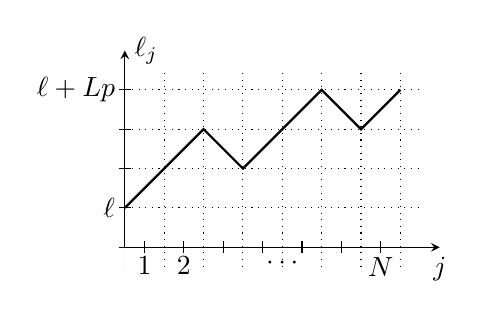
\begin{tikzpicture}[>=stealth]
     \draw[scale=0.5,thick] (0,0)--(2,2)--(3,1)--(5,3)--(6,2)--(7,3);
           
     \draw[<->] (0,2) -- (0,-0.5) -- (4,-0.5);
     \foreach \x in {0.25,0.75,...,3.25}
       \draw[xshift=\x cm,yshift=-0.5cm] (0,-0.075)--(0,0.075);
     
    \foreach \y in {-0.5,0,...,1.5}
       \draw[yshift=\y cm] (-0.075,0)--(0.075,0);
 
    \draw (0.25,-0.5) node[below] {$1$};
    \draw (0.75,-0.5) node[below] {$2$};
    \draw (2,-0.5) node[below] {$\cdots$};
    \draw (3.25,-0.5) node[below] {$N$};
    \draw (4,-0.5) node[below] {$j$};
    \draw (0,0) node [left] {$\ell$};
    \draw (0,1.5) node [left] {$\ell+Lp$};
    \draw (0,2) node [right] {$\ell_j$};
    \clip[scale=0.5] (0,-1.5) rectangle (7.5,3.5);
    \draw[scale=0.5,dotted] (-1,-2) grid (8,5);
  \end{tikzpicture}
}
  
\end{texexample}




%\begin{texexample}{Example}{}
%\newcommand{\ud}{\ensuremath \mathop{}\!\mathrm{d}}
%\(z=2\sin x\mathrm{d}x\) and \(z=2\sin x\ud x\)
%
%
%\newcommand{\ud}{\mathop{}\!\mathrm{d}}
%\bigskip
%
%It uses an empty operator and eliminates the space
%on its left with |\!|.
%
%Note the difference between
%
%\[z=2\sin x\mathrm{d}x  \]
%
%\[z=2\sin x\ud x\]
%
%where the diffrential is obtained respectively with
%|\mathrm{d}| and |\ud|.
%\end{texexample}




\subsubsection{God is in the details}

Sometimes you will be faced with small decisions for which the Journal style manual might not have an answer for you or the journal Editor might have a different opinion to yours. One such question is if one needs to insert the thousand separator in coefficients.

\[
\operatorname{erf}^{-1}(z)=\tfrac{1}{2}\sqrt{\pi}\left (z+\frac{\pi}{12}z^3+\frac{7\pi^2}{480}z^5+\frac{127\pi^3}{40320}z^7+\frac{4369\pi^4}{5806080}z^9+\frac{34807\pi^5}{182476800}z^{11}+\cdots\right )
\]


\[
\operatorname{erf}^{-1}(z)=\tfrac{1}{2}\sqrt{\pi}\left (z+\frac{\pi}{12}z^3+\frac{7\pi^2}{480}z^5+\frac{127\pi^3}{40,320}z^7+\frac{4,369\pi^4}{5,806,080}z^9+\frac{34,807\pi^5}{182{,}476,800}z^{11}+\cdots\right )
\]

\[
\operatorname{erf}^{-1}(z)=\tfrac{1}{2}\sqrt{\pi}\left (z+\frac{\pi}{12}z^3+\frac{7\pi^2}{480}z^5+\frac{127\pi^3}{40{,}320}z^7+\frac{4{,}369\pi^4}{5{,}806{,}080}z^9+\frac{34{,}807\pi^5}{182{,}476{,}800}z^{11}+\cdots\right )
\]



\[
\operatorname{erf}^{-1}(z)=\tfrac{1}{2}\sqrt{\pi}\left (z+\frac{\pi}{12}z^3+\frac{7\pi^2}{480}z^5+\frac{127\pi^3}{40\thinspace 320}z^7+\frac{4\thinspace 369\pi^4}{5\thinspace 806\thinspace 080}z^9+\frac{34\thinspace 807\pi^5}{182\thinspace 476\thinspace 800}z^{11}+\cdots\right )
\]


If you type the commas watch out to put them in |{,}| otherwise \tex's algorithm will leave a space. See the difference below:

\[182{,}476{,}800 \]
\[182,476,800\]

It is interesting to note that Knuth believes that in equations this is unnecessary.
He is quoted in Typesetting Mathematics.


\begin{quotation}
But where Don wrote 1000000 they substituted
1,000,000. Don objected that although this might be justifed in text, his use is perfectly OK in a formula. Well then, they replied, write \(10^6\).
Fine, said, Don, but what do I do 
when the number is 1234567? The IEEE standard here is to insert spaces, thus: 1 234 567.
Don doesn't like this in formulae, but agrees that it may be useful in a high precision context, such as numerical tables. 
\end{quotation}



The following are extracts from his paper \textit{Johann Faulhaber and Sums of Powers}:\footnote{\url{http://www-cs-faculty.stanford.edu/~uno/papers/jfsp.tex.gz}}

{
\[\vcenter{\halign{$#$\hfil\ &$#$\hfil\cr
\Sigma n^{11}&=39916800{n+6\choose 12}+
19958400{n+5\choose 10}+3160080{n+4\choose 8}
+168960{n+3\choose 6}\cr
\noalign{\smallskip}
&\qquad\null+2046{n+2\choose 4}+{n+1\choose 2}\,;\cr
\noalign{\smallskip}
\Sigma n^{13}&=6227020800{n+7\choose 14}+3632428800{n+6\choose 12}+
726485760{n+5\choose 10}\cr
\noalign{\smallskip}
&\qquad\null+57657600{n+4\choose 8}
+1561560{n+3\choose 6}+8190{n+2\choose 4}+\binom{n+1}{2}\,.\cr}}\]
}

Also, note in the last equation the use of a period at the end. 
This is something that evokes strong opinions and flaming wars in fora. 
I am not too sure if I agree on the last one, but the way that Knuth writes 
is very clear and his equations in a way are paragraphs. 
In this case the use of a period is recommended.


\subsection{Punctuation}
\index{maths>typography>punctuation}

There are two schools of thought when it comes to punctuation, that is punctuation in display style formulae. Some authors (Beccari, 2007) argue it is not necessary, others that it is necessary and essential \footcite{guiggiani2008}. Mermin \footcite{mermin89} strongly argued in his third rule that:  `The
Math Is Prose rule simply says: End
a displayed equation with a punctuation
mark. It is implicit in this
statement that the absence of a punctuation
mark is itself a degenerate
form of punctuation that, like periods,
commas or semicolons, can be used
provided it makes sense.''

The authors of this article believe that equations, both in display and text style, are part of the argumentation
and so punctuation should be used to help the reader. An example of good use of punctuation is:


Since
\[ a=b \]
and
\[ b=c,\]
it is proven that
\[ a =c. \]

It is extremely unusual to find an equation end with a question mark but here is one. What is 
\[ a = d^2\mathrm{?} \]

If you do put a question mark or an exclamation mark and you are using unicode fonts,
you will need to use |\mathrm{?}| not to confuse it with the relevant symbols.

Most journals require that equations be punctuated, like normal text. Even if the author of the manuscript disagrees, probably the journal editor will add the punctuation.

Read your mathematical text aloud and introduce punctuation as if it was spelled in words rather than mathematical symbols. 

\subsection{Numbering Equations}
\index{maths>typography>equation numbering}

One question that you may face is the numbering of display equations. Early books used numbering sparingly, whereas many authors go overboard and number all the equations.

According to Knuth et al:\footnote{\url{http://tex.loria.fr/typographie/mathwriting.pdf}}
Numbering all displayed formulas is usually a bad idea; number the important ones only.

Halmos\footnote{\url{http://www.math.uh.edu/~tomforde/Books/Halmos-How-To-Write.pdf}} offers pretty much the same good advice,

\begin{latexquotation}
What about ``inequality (*)", or ``equation (7)", or ``formula (iii)"; should all displays be labelled or numbered? My answer is no. Reason: just as you shouldn't mention irrelevant assumptions or name irrelevant concepts, you also shouldn't attach irrelevant labels. Some small part of the reader's attention is attracted to the label, and some small part of his mind will wonder why the label is there. If there is a reason, then the wonder serves a healthy purpose by way of preparation, with no fuss, for a future reference to the same idea; if there is no reason, then the attention and the wonder were wasted.
\end{latexquotation}

Mermin's argues in his Good samaritan Rule: that it is distressing to having to hunt for an equation back in a manuscript for Eq. (2.46) not because your subsequent progress requires
you to inspect it in detail, but merely to find out what it is about so
you may know the principles that go into the construction of Eq. (7.38).
The Good Samaritan rule says: When referring to an equation identify it by
a phrase as well as a number. No compassionate and helpful person
would herald the arrival of Eq. (7.38) by saying "inserting (2.47) and (3.51)
into (5.13)..." when it is possible to say "inserting the form (2.47) of the
electric field $E$ and the Lindhard form (3.51) of the dielectric function $e$ into
the constitutive equation (5.13). To be sure, it's longer this way but much 
clearer\ldots'

For those that want only the equations that are referenced numbered the package \pkgname{autoref} can automate this. This is not included in this package due to conflicts with \pkgname{mathtools} and \pkgname{amsmath}.
\footnote{See also discussion at \protect\url{http://tex.stackexchange.com/questions/29267/which-equations-should-be numbered/49080\#49080}}

Now if you wish to argue about this is fine.

\section{Mathmode}

\tex is in \textit{mathmode} when it is reading mathematics. The |ifmmode| can be used to find out if \tex is in math mode. It denotes the start of an if-then-else control structure that tests whether \tex is currently in either math mode or display math mode. The |\else| part is optional. <TeX code 1> is processed if TeX is in one of the math modes, otherwise it is ignored. 
If the |\else| section is included and TeX is not in one of the math modes then \meta{TeX code 2} is processed; otherwise it is ignored.


\begin{texexample}{Calligraphic fonts}{ex:cal}

\newcommand{\Acal}{\ifmmode \mathcal{Acal} \else \(\mathcal{Acal}\) \fi}
The commandd efines a macro |\Acal| that can be used both in and out of math mode to typeset a calligraphy script A. 

This is a calligraphic {\Acal} or ({\Acal}).
\end{texexample}


\section{Useful packages}

Besides the main packages that we have discussed so far and which should be in everyone's toolbox, there are a number of other packages that you may find useful. One such package is the \pkgname{multienum}, which although not really a packaged specializing in mathematical typesetting, it provides an environment to set multiple equations, as in an exercise or exam.



\subsection{the multienum package}

The \docpkg{multienum} enables  the typestting of multiple equations on one line and numbering them, either with roman, arabic or alpha letters.

\emphasis{usepackage, multienum,begin,end,multienumerate}
\begin{teXXX}
\documentclass{article}
\usepackage{multienum}
\renewcommand{\regularlisti}{\setcounter{multienumi}{0}%
  \renewcommand{\labelenumi}%
  {\addtocounter{multienumi}{1}\alph{multienumi})}}
\begin{document}
\begin{multienumerate}[oddlist]
\mitemxxx{\(x^2 + y^2 = 1\)}{\(a + b = c\)}{\(r-x = y+z\)}
\mitemxxx{\(f - y = z\)}{\(a - b = 2d\)}{\(r+x = 2y-3z\)}
\end{multienumerate}
\end{document}
\end{teXXX}


\begin{multienumerate}[oddlist]
\mitemxxx{\(x^2 + y^2 = 1\)}{\(a + b = c\)}{\(r-x = y+z\)}
\end{multienumerate}
\begin{multienumerate}[evenlist]
\mitemxxx{\(f - y = z\)}{\(a - b = 2d\)}{\(r+x = 2y-3z\)}
\end{multienumerate}


\hrule

\bigskip

We can also enumerate the items using an even-only or odd only
counter.
\subsection*{Answers to Even-Numbered Exercises}
\begin{multienumerate}[evenlist]
\mitemxxxx{Not}{Linear}{Not}{Quadratic}
\mitemxxxo{Not}{Linear}{No; if $x=3$, then $y=-2$.}
\mitemxx{$(x_1,x_2)=(2+\frac{1}{3}t,t)$ or
$(s,3s-6)$}{$(x_1,x_2,x_3)=(2+\frac{5}{2}s-3t,s,t)$}
\mitemx{$(x_1,x_2,x_3,x_4)= (\frac{1}{4}+\frac{5}{4}s+\frac{3}{4}t-u,s,t,u)$
or $(s,t,u,\frac{1}{4}-s+\frac{5}{4}t+\frac{3}{4}u)$}
\mitemxxxx{$(2,-1,3)$}{None}{$(2,1,0,1)$}{$(0,0,0,0)$}
\end{multienumerate}
\bigskip



\newcommand\thecasestudylabel{Case Study}
\newenvironment{casestudy}[2][]{%
   \clearpage\par\leavevmode
   \addcontentsline{toc}{section}{\thecasestudylabel:  #1}
    \topline\vskip1.5pt
   {\noindent\large CASE STUDY\par}\vspace{3.5pt}
   \noindent\textsc{\large#1}\par
   \bigskip
   {#2}
   \medskip
   \topline
}{%
\vfill\bottomline}

\begin{casestudy}[The Riemann hypothesis.]{%
Typeset the text and the equations, shown below. Use a standard minimal to achieve it. Note the fraktur fonts. Text must all be as one paragraph.}

It is well known that the Riemann zeta function $\zeta(s)$ of a complex variable $s=\sigma+it$ is defined by
\[
\zeta(s)=\sum_{n=1}^{\infty}\frac{1}{n^{s}}
\]
for the real part $\mathfrak{R}(s)>1$ and its analytic continuation in the half plane $\sigma>0$ is
\begin{equation}\label{func:zeta}
\zeta(s)=\sum_{n=1}^{N}\frac{1}{n^{s}}-\frac{N^{1-s}}{1-s}-\frac{1}{2}N^{-s}
+s\int_{N}^{\infty}\frac{\frac{1}{2}-\{x\}}{x^{s+1}}dx
\end{equation}
for any integer $N\geq1$ and $\mathfrak{R}(s)>0$.
It extends to an analytic function in the whole complex plane except for having a simple pole at $s=1$. Trivially, $\zeta(-2n)=0$ for all positive integers. All other zeros of the Riemann zeta functions are called its nontrivial zeros.
\bottomline

\begin{teX}
It is well known that the Riemann zeta function $\zeta(s)$ of a complex variable $s=\sigma+it$ is defined by
\[
\zeta(s)=\sum_{n=1}^{\infty}\frac{1}{n^{s}}
\]
for the real part $\mathfrak{R}(s)>1$ and its analytic continuation in the half plane $\sigma>0$ is
\begin{equation}\label{func:zeta}
\zeta(s)=\sum_{n=1}^{N}\frac{1}{n^{s}}-\frac{N^{1-s}}{1-s}-\frac{1}{2}N^{-s}
+s\int_{N}^{\infty}\frac{\frac{1}{2}-\{x\}}{x^{s+1}}dx
\end{equation}
for any integer $N\geq1$ and $\mathfrak{R}(s)>0$.
It extends to an analytic function in the whole complex plane except for having a simple pole at $s=1$. Trivially, $\zeta(-2n)=0$ for all positive integers. All other zeros of the Riemann zeta functions are called its nontrivial zeros.
\end{teX}

Please note that the maths and the text, are typed as a single block. Do not leave any spaces in between. We have used |\mathfrak| for the fraktur font. We have also used $it$ for the imaginary part. This would depend on the style used in your field. 
\end{casestudy}

\clearpage
\section{Gather}

\begin{docEnvironment}{gather}{}
This is like a multi line environment with no special horizontal alignment. All rows
are centered and can have an own equation number:
\end{docEnvironment}

\begin{texexample}{Gather}{ex:gather}
\begingroup
\def\O{\mathcal{O}}
\begin{gather}
 \O,\O(E_4),\O(E_2),\O(H-E_3-E_5),\O(H-E_3),\O(H-E_5),\\ 
\O(2H-E_1-E_3-E_5-E_6),\O(2H-E_1-E_3-E_5),\O(2H-E_3-E_5-E_6).
\end{gather}

So lautet der Beweis des Satzes $2 \times 2 = 4$:
\begin{gather}
(\Omega^{\nu})^{\mu}{}'x = \Omega^{\nu \times \mu}{}'x \text{ Def.}\\
%\begin{split}
\Omega^{2 \times 2}{}'x = (\Omega^{2})^{2}{}'x = (\Omega^{2})^{1 + 1}{}'x = \Omega^{2}{}'\Omega^{2}{}'x = \Omega^{1 + 1}{}'\Omega^{1 + 1}{}'x\nonumber \\
= (\Omega'\Omega)'(\Omega'\Omega)'x = \Omega'\Omega'\Omega'\Omega'x = \Omega^{1 + 1 + 1 + 1}{}'x = \Omega^{4}{}'x.
%\end{split}
\end{gather}


\begin{gather*}
  x = \Omega^{0}{}' x \text{ Def.\ and}\\
  \Omega'\Omega^{\nu}{}'x = \Omega^{\nu+1}{}'x \text{ Def.}
\end{gather*}
\begin{equation}
  x = \Omega^{0}{}' x \text{ Def.\ and}\\
\Omega'\Omega^{\nu}{}'x = \Omega^{\nu+1}{}'x \text{ Def.}
\end{equation}
\endgroup
\end{texexample}


\section{How to number equations either to the left or right?}
\label{eqnochange}

\latexe uses Plain TeX \docAuxCommand{eqno} and \docAuxCommand{leqno} to place the equation number either to the left or the right of the equation. The placement is done automatically and the recommended way is to set this through the documentclass declaration at the start of the document. This can also be set manually later on through the above control sequences, as shown in the Example~\ref{ex:eqno}.

\begin{texexample}{Left or right numbering}{ex:eqno}
\makeatletter
\[ a = b + x^2 \eqno \@eqnnum \]
or at left
\[ a = b + x^2 \leqno \@eqnnum \]
\makeatother
\end{texexample}


%\meaning\text

%\chapter{Unicode Math}
\tcbdocmarginnote{N 29-06-2018}
Unicode contains separate codepoints for most if not all variations of alphabet
shape one may wish to use in mathematical notation. The complete list is shown
in table 5. Some of these have been covered in the previous sections.
The math font switching commands do not nest; therefore if you want sans
serif bold, you must write |\mathbfsf{...}| rather than |\mathbf{\mathsf{...}}|.
This may change in the future.

\section{Unicode maths font setup}

The promise of Unicode is that all symbols and alphabetic variants are in one font. The \pkgname{unicode-math}
maps all the available unicode math characters of a math font to respective \latex commands. If you have patience you can actually input them directly from the keyboard rather than in commands.

The best advice that I can give you is to read the \pkgname{unicode-math} carefully. 

\begin{docCommand} {setmathfont} { \oarg{range=\meta{unicode range}, \meta{font features } } \marg{font name} }
In many cases using one font might not be adequate. Specific Unicode ranges can be assigned to separate fonts.
\end{docCommand}

\subsection{Control over maths alphabets}

\subsection{Math `versions'}

\subsection{Maths input}

\subsection{Math `style'}

\subsubsection{Bold style}

Similar as in the previous section, ISO standards differ somewhat to \tex’s conventions
(and classical typesetting) for ‘boldness’ in mathematics. In the past, it has
been customary to use bold upright letters to denote things like vectors and matrices.


$$\boldsymbol{\omega} \times \mathbf{T} = \mathbf{T'}$$

$$\mathbf{\omega} = {1\over 2}\kappa \mathbf{B} + {1\over 2}(\kappa \mathbf{B} + \tau \mathbf{T}) + {1\over 2}\tau \mathbf{T} = \kappa \mathbf{B} + \tau \mathbf{T}
$$

\[
\mathbf{e} = \frac{\mathbf{A}}{m k} = \frac{1}{m k}(\mathbf{p} \times \mathbf{L})
\]

\subsubsection{Sans serif style}

\subsubsection{Blackboard or double-struck}



\subsubsection{Caligraphic and Script variants}



\section{Growing and non-growing accents}

This are the most problematic with Unicode fonts.

%%%%%%%% INPUT INTEGRAL FILES %%%%%%%%%%
%%%%%%%%%%%%%%%%%%%%%%%%%%%%%%%
 %% Too many errors here need to revisit.
 \subsection{Delimiters}
 \begin{multicols}{2}
% \showmbrace/{002F}{}
% \showlbrace({0028}{}
% \showlbrace[{005B}{}
% \showlbrace\lbrace{007B}{}
% \showmbrace\backslash{005C}{}
% \showrbrace){0029}{}
% \showrbrace]{005D}{}
% \showrbrace\rbrace{007D}{}
% \showlbrace\lceil{2308}{}
% \showlbrace\lfloor{230A}{}
% \showlbrace\lmoustache{23B0}{*}
% \showlbrace\lbrbrak{2772}{*}
% \showlbrace\lBrack{27E6}{*}
% \showlbrace\langle{27E8}{}, \cmd<
% \showlbrace\lAngle{27EA}{*}
% \showlbrace\lgroup{27EE}{*}
% \showlbrace\lBrace{2983}{*}
% \showlbrace\lParen{2985}{*}
% \showrbrace\rceil{2309}{}
 %\showrbrace\rfloor{230B}{}
% \showrbrace\rmoustache{23B1}{*}
% \showrbrace\rbrbrak{2773}{*}
% \showrbrace\rBrack{27E7}{*}
% \showrbrace\rangle{27E9}{}, \cmd>
% \showrbrace\rAngle{27EB}{*}
% \showrbrace\rgroup{27EF}{*}
 %\showrbrace\rBrace{2984}{*}
% \showrbrace\rParen{2986}{*}
 \end{multicols}

 \begin{multicols}{2}
% \showmbrace\vert{007C}{}, \cmd|
 \showmbrace\Vert{2016}{*}, \cmd\|
 \showmbrace\Vvert{2980}{}
 \showmbrace\uparrow{2191}{}
 \showmbrace\downarrow{2193}{}
 \showmbrace\updownarrow{2195}{}
 \showmbrace\Uparrow{21D1}{}
 \showmbrace\Downarrow{21D3}{}
 \showmbrace\Updownarrow{21D5}{}
% \showmbrace\Uuparrow{290A}{*}
% \showmbrace\Ddownarrow{290B}{*}
% \showmbrace\UUparrow{27F0}{*}
% \showmbrace\DDownarrow{27F1}{*}
% \showmbrace\arrowvert{XXXX}{}
% \showmbrace\Arrowvert{XXXX}{}
% \showmbrace\bracevert{XXXX}{*}
 \end{multicols}

 \subsection{Other bracess}
 \begin{multicols}{2}
 \showsymbol\ulcorner{231C}{*}
 \showsymbol\urcorner{231D}{*}
 \showsymbol\llcorner{231E}{*}
 \showsymbol\lrcorner{231F}{*}
 \showsymbol\Lbrbrak{27EC}{*}
 \showsymbol\Rbrbrak{27ED}{*}
 \showsymbol\llparenthesis{2987}{*}
 \showsymbol\rrparenthesis{2988}{*}
 \showsymbol\llangle{2989}{*}
 \showsymbol\rrangle{298A}{*}
 \showsymbol\lbrackubar{298B}{*}
 \showsymbol\rbrackubar{298C}{*}
 \showsymbol\lbrackultick{298D}{*}
 \showsymbol\rbracklrtick{298E}{*}
 \showsymbol\lbracklltick{298F}{*}
 \showsymbol\rbrackurtick{2990}{*}
 \showsymbol\langledot{2991}{*}
 \showsymbol\rangledot{2992}{*}
 \showsymbol\lparenless{2993}{*}
 \showsymbol\rparengtr{2994}{*}
 \showsymbol\Lparengtr{2995}{*}
 \showsymbol\Rparenless{2996}{*}
 \showsymbol\lblkbrbrak{2997}{*}
 \showsymbol\rblkbrbrak{2998}{*}
 \showsymbol\lvzigzag{29D8}{*}
 \showsymbol\rvzigzag{29D9}{*}
 \showsymbol\Lvzigzag{29DA}{*}
 \showsymbol\Rvzigzag{29DB}{*}
 \showsymbol\lcurvyangle{29FC}{*}
 \showsymbol\rcurvyangle{29FD}{*}
 \showsymbol\lbrbrak{2772}{*}
 \showsymbol\rbrbrak{2773}{*}
 \showsymbol\lbag{27C5}{*}
 \showsymbol\rbag{27C6}{*}
 \showsymbol\Lbrbrak{27EC}{*}
 \showsymbol\Rbrbrak{27ED}{*}
 \end{multicols}

 \section{Alphabetics}
 \begin{multicols}{2}
\showsymbolalpha\Gamma{0393}{}
\showsymbolalpha\Delta{0394}{}
\showsymbolalpha\Theta{0398}{}
\showsymbolalpha\Lambda{039B}{}
\showsymbolalpha\Xi{039E}{}
\showsymbolalpha\Pi{03A0}{}
\showsymbolalpha\Sigma{03A3}{}
\showsymbolalpha\Upsilon{03A5}{}
\showsymbolalpha\Phi{03A6}{}
\showsymbolalpha\Psi{03A8}{}
\showsymbolalpha\Omega{03A9}{}
\showsymbolalpha\alpha{03B1}{}
\showsymbolalpha\beta{03B2}{}
\showsymbolalpha\gamma{03B3}{}
\showsymbolalpha\delta{03B4}{}
\showsymbolalpha\epsilon{03B5}{}
\showsymbolalpha\zeta{03B6}{}
\showsymbolalpha\eta{03B7}{}
\showsymbolalpha\theta{03B8}{}
\showsymbolalpha\iota{03B9}{}
\showsymbolalpha\kappa{03BA}{}
\showsymbolalpha\lambda{03BB}{}
\showsymbolalpha\mu{03BC}{}
\showsymbolalpha\nu{03BD}{}
\showsymbolalpha\xi{03BE}{}
\showsymbolalpha\pi{03C0}{}
\showsymbolalpha\rho{03C1}{}
\showsymbolalpha\sigma{03C3}{}
\showsymbolalpha\tau{03C4}{}
\showsymbolalpha\upsilon{03C5}{}
\showsymbolalpha\phi{03D5}{}
\showsymbolalpha\chi{03C7}{}
\showsymbolalpha\psi{03C8}{}
\showsymbolalpha\omega{03C9}{}
\showsymbolalpha\varepsilon{03F5}{}
\showsymbolalpha\vartheta{03D1}{}
\showsymbolalpha\varpi{03D6}{}
\showsymbolalpha\varrho{03F1}{}
\showsymbolalpha\varsigma{03C2}{}
\showsymbolalpha\varphi{03C6}{}
\showsymbolalpha\nabla{2207}{}
\showsymbolalpha\partial{2202}{}
\showsymbolalpha\imath{1D6A4}{}
\showsymbolalpha\jmath{1D6A5}{}
 \end{multicols}
% \subsection{Accents}
 \begin{multicols}{2}
 \showaccent\grave{0300}{}
 \showaccent\acute{0301}{}
 \showaccent\hat{0302}{}
 \showaccent\tilde{0303}{}
 \showaccent\bar{0304}{}
 \showaccent\breve{0306}{}
 \showaccent\dot{0307}{}
 \showaccent\ddot{0308}{}
 \showaccent\ovhook{0309}{}
 \showaccent\mathring{030A}{}
 \showaccent\check{030C}{}
 \showaccent\candra{0310}{}
 \showaccent\oturnedcomma{0312}{}
 \showaccent\ocommatopright{0315}{}
 \showaccent\droang{031A}{}
 \showaccent\leftharpoonaccent{20D0}{}
 \showaccent\rightharpoonaccent{20D1}{}
 %\showaccent\leftarrowaccent{20D6}{}
 \showaccent\vec{20D7}{}, \cmd\rightarrowaccent
 %\showaccent\leftrightarrowaccent{20E1}{}
 \showaccent\dddot{20DB}{}
 \showaccent\ddddot{20DC}{}
 \showaccent\annuity{20E7}{}
 \showaccent\widebridgeabove{20E9}{}
 \showaccent\asteraccent{20F0}{}
 \end{multicols}

 \begin{multicols}{2}
 \showwideaccent\widehat{0302}{*}
 \showwideaccent\widetilde{0303}{*}
% \showwideaccent\widecheck{030C}{*}
 \showwideaccent\overleftarrow{20D6}{}
 \showwideaccent\overrightarrow{20D7}{}
 \showwideaccent\underrightarrow{20EF}{}
 \showwideaccent\underleftarrow{20EE}{}
 \showwideaccent\overleftrightarrow{20E1}{}
 \showwideaccent\underleftrightarrow{034D}{}
% \showwideaccent\overleftharpoon{20D0}{}
% \showwideaccent\overrightharpoon{20D1}{}
% \showwideaccent\underleftharpoon{20EC}{}
% \showwideaccent\underrightharpoon{20ED}{}
 \end{multicols}

 OpenType STIX fonts include a number of under accents that can be used in
 math mode, but \TeX\ does not support under accents natively so such glyphs
 can not be used directly. Under accents can be set using regular accents and
 commands like |\underaccent| from the \pkgname{accents} package, for example
 gives |\(\underaccent{\hat}{X}\)|. The
 \pkgname{undertilde} package provides |\utilde| for extensible under tilde
 accent \citep{undertilde}.
 
 
 % \subsection{Over and under brackets}
 \begin{multicols}{2}
 %\showover\overbracket{23B4}{} conflict mathtools consider remove mathtools for UNICODE
 \showover\overparen{23DC}{}
 \showover\overbrace{23DE}{}
 \showover\underbracket{23B5}{} %conflict mathtools?
 \showover\underparen{23DD}{}
 \showover\underbrace{23DF}{}
 \end{multicols}

 \subsection{Radicals}
 \begin{multicols}{2}
 \showaccent\sqrt{221A}{}
 \showaccent\longdivision{27CC}{*}
 \end{multicols}
 
 
 
 
 
 
 \subsection{Big operators}
 \begin{multicols}{2}
 \showop\Bbbsum{2140}{}
 \showop\prod{220F}{}
 \showop\coprod{2210}{}
 \showop\sum{2211}{}
 \showop\bigwedge{22C0}{}
 \showop\bigvee{22C1}{}
 \showop\bigcap{22C2}{}
 \showop\bigcup{22C3}{}
 \showop\leftouterjoin{27D5}{*}
 \showop\rightouterjoin{27D6}{*}
 \showop\fullouterjoin{27D7}{*}
 \showop\bigbot{27D8}{*}
 \showop\bigtop{27D9}{*}
 \showop\xsol{29F8}{*}
 \showop\xbsol{29F9}{*}
 \showop\bigodot{2A00}{*}
 \showop\bigoplus{2A01}{*}
 \showop\bigotimes{2A02}{*}
 \showop\bigcupdot{2A03}{*}
 \showop\biguplus{2A04}{*}
 \showop\bigsqcap{2A05}{*}
 \showop\bigsqcup{2A06}{*}
 \showop\conjquant{2A07}{*}
 \showop\disjquant{2A08}{*}
 \showop\bigtimes{2A09}{*}
 \showop\modtwosum{2A0A}{*}
 \showop\Join{2A1D}{*}
 \showop\bigtriangleleft{2A1E}{*}
 \showop\zcmp{2A1F}{*}
 \showop\zpipe{2A20}{*}
 \showop\zproject{2A21}{*}
 \showop\biginterleave{2AFC}{}
 \showop\bigtalloblong{2AFF}{*}
 \end{multicols}
 
 \section{General manipulations test.}
 
 Here are some examples using big operators

$$\sum_{n=s}^t C\cdot f(n) = C\cdot \sum_{n=s}^t f(n),$$ where ``'C'' is a constant

\[\sum_{n=s}^t f(n) + \sum_{n=s}^{t} g(n) = \sum_{n=s}^t \left[f(n) + g(n)\right]\] 

\[\sum_{n=s}^t f(n) - \sum_{n=s}^{t} g(n) = \sum_{n=s}^t \left[f(n) - g(n)\right]\] 

\[\sum_{n=s}^t f(n) = \sum_{n=s+p}^{t+p} f(n-p) \] 

\[\sum_{n\in B} f(n) = \sum_{m\in A} f(\sigma(m)),\] for a bijection σ from a finite set ``$A$'' onto a finite set ``$B$''; this generalizes the preceding formula.

\[\sum_{n=s}^j f(n) + \sum_{n=j+1}^t f(n) = \sum_{n=s}^t f(n)\] 

\[\sum_{i=k_0}^{k_1}\sum_{j=l_0}^{l_1} a_{i,j} = \sum_{j=l_0}^{l_1}\sum_{i=k_0}^{k_1} a_{i,j}\] 

\[\sum_{k\le j \le i\le n} a_{i,j} = \sum_{i=k}^n\sum_{j=k}^i a_{i,j} = \sum_{j=k}^n\sum_{i=j}^n a_{i,j}\] 


\[\sum_{n=0}^t f(2n) + \sum_{n=0}^t f(2n+1) = \sum_{n=0}^{2t+1} f(n)\] 

\[\sum_{n=0}^t \sum_{i=0}^{z-1} f(z\cdot n+i) = \sum_{n=0}^{z\cdot t+z-1} f(n)\] 

\[\sum_{i=s}^m\sum_{j=t}^n {a_i}{c_j} = \sum_{i=s}^m a_i \cdot \sum_{j=t}^n c_j\] 

\[\sum_{n=s}^t \ln f(n) = \ln \prod_{n=s}^t f(n)\] 

\[c^{\left[\sum_{n=s}^t f(n) \right]} = \prod_{n=s}^t c^{f(n)}\] 
 
 
 \section{Convergence criteria}
 
The product of positive real numbers

\[\prod_{n=1}^{\infty} a_n\]
converges to a nonzero real number if and only if the sum
\[\sum_{n=1}^{\infty} \log(a_n)\]
converges. This allows the translation of convergence criteria for infinite sums into convergence criteria for infinite products. The same criterion applies to products of arbitrary complex numbers (including negative reals) if log is understood as a fixed Complex logarithm which satisfies $\log(1) = 0$, with the proviso that the infinite product diverges when infinitely many ''$a_n$'' fall outside 
the domain of log, whereas finitely many such ''$a_n$'' can be ignored in the sum.

For products of reals in which each $a_n\ge1$, written as, for instance, $a_n=1+p_n$,
where $p_n\ge 0$, the bounds

\[1+\sum_{n=1}^{N} p_n \le \prod_{n=1}^{N} \left( 1 + p_n \right) \le \exp \left( \sum_{n=1}^{N}p_n \right)\]

show that the infinite product converges precisely if the infinite sum of the $p_n$ converges. This relies on the Monotone convergence theorem. More generally, the convergence of $\prod_{n=1}^\infty(1+p_n)$ is equivalent to the convergence of $\sum_{n=1}^\infty p_n$ 
%if ''p<sub>n</sub>'' are real or complex numbers such that <math>\sum_{n=1}^\infty|p_n|^2<+\infty\], since <math>\log(1+x)=x+O(x^2)\] in a neighbourhood of 0.
%
%If the series ''p''<sub>''n''</sub> diverges, then the sequence of partial products converges to zero as a sequence.  The infinite product is said to '''diverge to zero'''.
% 
 
 
 
 
 
 
 
 
%% Relations symbols from STIX font
%% 
  \subsection{Relations}
 \begin{multicols}{2}
% \showrelsymbol*{002A}{}, \cmd\ast
% \showrelsymbol:{003A}{}
 \showrelsymbol{\less}{003C}{}, \cmd\less
 \showrelsymbol{\equal}{003D}{}, \cmd\equal
 \showrelsymbol{\greater}{003E}{}, \cmd\greater
 \showrelsymbol\closure{2050}{*}
 %\showrelsymbol\vertoverlay{20D2}{}
 \showrelsymbol\leftarrow{2190}{}, \cmd\gets
 \showrelsymbol\uparrow{2191}{}
 \showrelsymbol\rightarrow{2192}{}, \cmd\to
 \showrelsymbol\downarrow{2193}{}
 \showrelsymbol\leftrightarrow{2194}{}
 \showrelsymbol\updownarrow{2195}{}
 \showrelsymbol\nwarrow{2196}{}
 \showrelsymbol\nearrow{2197}{}
 \showrelsymbol\searrow{2198}{}
 \showrelsymbol\swarrow{2199}{}
 \showrelsymbol\nleftarrow{219A}{}
 \showrelsymbol\nrightarrow{219B}{}
 \showrelsymbol\leftwavearrow{219C}{}
 \showrelsymbol\rightwavearrow{219D}{}
 \showrelsymbol\twoheadleftarrow{219E}{}
 \showrelsymbol\twoheaduparrow{219F}{}
 \showrelsymbol\twoheadrightarrow{21A0}{}
 \showrelsymbol\twoheaddownarrow{21A1}{}
 \showrelsymbol\leftarrowtail{21A2}{}
 \showrelsymbol\rightarrowtail{21A3}{}
 \showrelsymbol\mapsfrom{21A4}{}
 \showrelsymbol\mapsup{21A5}{}
 \showrelsymbol\mapsto{21A6}{}
 \showrelsymbol\mapsdown{21A7}{}
 \showrelsymbol\hookleftarrow{21A9}{}
 \showrelsymbol\hookrightarrow{21AA}{}
 \showrelsymbol\looparrowleft{21AB}{}
 \showrelsymbol\looparrowright{21AC}{}
 \showrelsymbol\leftrightsquigarrow{21AD}{}
 \showrelsymbol\nleftrightarrow{21AE}{}
 \showrelsymbol\downzigzagarrow{21AF}{}
 \showrelsymbol\Lsh{21B0}{}
 \showrelsymbol\Rsh{21B1}{}
 \showrelsymbol\Ldsh{21B2}{}
 \showrelsymbol\Rdsh{21B3}{}
 \showrelsymbol\curvearrowleft{21B6}{}
 \showrelsymbol\curvearrowright{21B7}{}
 \showrelsymbol\circlearrowleft{21BA}{}
 \showrelsymbol\circlearrowright{21BB}{}
 \showrelsymbol\leftharpoonup{21BC}{}
 \showrelsymbol\leftharpoondown{21BD}{}
 \showrelsymbol\upharpoonright{21BE}{}, \cmd\restriction
 \showrelsymbol\upharpoonleft{21BF}{}
 \showrelsymbol\rightharpoonup{21C0}{}
 \showrelsymbol\rightharpoondown{21C1}{}
 \showrelsymbol\downharpoonright{21C2}{}
 \showrelsymbol\downharpoonleft{21C3}{}
 \showrelsymbol\rightleftarrows{21C4}{}
 \showrelsymbol\updownarrows{21C5}{}
 \showrelsymbol\leftrightarrows{21C6}{}
 \showrelsymbol\leftleftarrows{21C7}{}
 \showrelsymbol\upuparrows{21C8}{}
 \showrelsymbol\rightrightarrows{21C9}{}
 \showrelsymbol\downdownarrows{21CA}{}
 \showrelsymbol\leftrightharpoons{21CB}{}
 \showrelsymbol\rightleftharpoons{21CC}{}
 \showrelsymbol\nLeftarrow{21CD}{}
 \showrelsymbol\nLeftrightarrow{21CE}{}
 \showrelsymbol\nRightarrow{21CF}{}
 \showrelsymbol\Leftarrow{21D0}{}
 \showrelsymbol\Uparrow{21D1}{}
 \showrelsymbol\Rightarrow{21D2}{}
 \showrelsymbol\Downarrow{21D3}{}
 \showrelsymbol\Leftrightarrow{21D4}{}
 \showrelsymbol\Updownarrow{21D5}{}
 \showrelsymbol\Nwarrow{21D6}{}
 \showrelsymbol\Nearrow{21D7}{}
 \showrelsymbol\Searrow{21D8}{}
 \showrelsymbol\Swarrow{21D9}{}
 \showrelsymbol\Lleftarrow{21DA}{*}
 \showrelsymbol\Rrightarrow{21DB}{*}
 \showrelsymbol\leftsquigarrow{21DC}{}
 \showrelsymbol\rightsquigarrow{21DD}{}, \cmd\leadsto
 \showrelsymbol\barleftarrow{21E4}{*}
 \showrelsymbol\rightarrowbar{21E5}{*}
 \showrelsymbol\circleonrightarrow{21F4}{*}
 \showrelsymbol\downuparrows{21F5}{}
 \showrelsymbol\rightthreearrows{21F6}{*}
 \showrelsymbol\nvleftarrow{21F7}{*}
 \showrelsymbol\nvrightarrow{21F8}{*}
 \showrelsymbol\nvleftrightarrow{21F9}{*}
 \showrelsymbol\nVleftarrow{21FA}{*}
 \showrelsymbol\nVrightarrow{21FB}{*}
 \showrelsymbol\nVleftrightarrow{21FC}{*}
 \showrelsymbol\leftarrowtriangle{21FD}{*}
 \showrelsymbol\rightarrowtriangle{21FE}{*}
 \showrelsymbol\leftrightarrowtriangle{21FF}{*}
 \showrelsymbol\in{2208}{}
 \showrelsymbol\notin{2209}{}
 \showrelsymbol\smallin{220A}{}
 \showrelsymbol\ni{220B}{}, \cmd\owns
 \showrelsymbol\nni{220C}{}
 \showrelsymbol\smallni{220D}{}
 \showrelsymbol\propto{221D}{}
 \showrelsymbol\varpropto{221D}{}
 \showrelsymbol\mid{2223}{}
 \showrelsymbol\shortmid{2223}{}
 \showrelsymbol\nmid{2224}{}
 \showrelsymbol\nshortmid{2224}{*}
 \showrelsymbol\parallel{2225}{}
 \showrelsymbol\shortparallel{2225}{*}
 \showrelsymbol\nparallel{2226}{}
 \showrelsymbol\nshortparallel{2226}{*}
 \showrelsymbol\Colon{2237}{}
 \showrelsymbol\dashcolon{2239}{}
 \showrelsymbol\dotsminusdots{223A}{}
 \showrelsymbol\kernelcontraction{223B}{}
 \showrelsymbol\sim{223C}{}
 \showrelsymbol\thicksim{223C}{}
 \showrelsymbol\backsim{223D}{}
 \showrelsymbol\nsim{2241}{}
 \showrelsymbol\eqsim{2242}{}
 \showrelsymbol\simeq{2243}{}
 \showrelsymbol\nsime{2244}{}
 \showrelsymbol\cong{2245}{}
 \showrelsymbol\simneqq{2246}{}
 \showrelsymbol\ncong{2247}{}
 \showrelsymbol\approx{2248}{}
 \showrelsymbol\thickapprox{2248}{}
 \showrelsymbol\napprox{2249}{}
 \showrelsymbol\approxeq{224A}{}
 \showrelsymbol\approxident{224B}{}
 \showrelsymbol\backcong{224C}{}
 \showrelsymbol\asymp{224D}{}
 \showrelsymbol\Bumpeq{224E}{}
 \showrelsymbol\bumpeq{224F}{}
 \showrelsymbol\doteq{2250}{}
 \showrelsymbol\Doteq{2251}{}, \cmd\doteqdot
 \showrelsymbol\fallingdotseq{2252}{}
 \showrelsymbol\risingdotseq{2253}{}
 \showrelsymbol\coloneq{2254}{}
 \showrelsymbol\eqcolon{2255}{}
 \showrelsymbol\eqcirc{2256}{}
 \showrelsymbol\circeq{2257}{}
 \showrelsymbol\arceq{2258}{}
 \showrelsymbol\wedgeq{2259}{}
 \showrelsymbol\veeeq{225A}{}
 \showrelsymbol\stareq{225B}{}
 \showrelsymbol\triangleq{225C}{}
 \showrelsymbol\eqdef{225D}{}
 \showrelsymbol\measeq{225E}{}
 \showrelsymbol\questeq{225F}{}
 \showrelsymbol\ne{2260}{}, \cmd\neq
 \showrelsymbol\equiv{2261}{}
 \showrelsymbol\nequiv{2262}{}
 \showrelsymbol\Equiv{2263}{}
 \showrelsymbol\leq{2264}{}, \cmd\le
 \showrelsymbol\geq{2265}{}, \cmd\ge
 \showrelsymbol\leqq{2266}{}
 \showrelsymbol\geqq{2267}{}
 \showrelsymbol\lneqq{2268}{}
 \showrelsymbol\lvertneqq{2268}{}
 \showrelsymbol\gneqq{2269}{}
 \showrelsymbol\gvertneqq{2269}{}
 \showrelsymbol\ll{226A}{}
 \showrelsymbol\gg{226B}{}
 \showrelsymbol\between{226C}{}
 \showrelsymbol\nasymp{226D}{}
 \showrelsymbol\nless{226E}{}
 \showrelsymbol\ngtr{226F}{}
 \showrelsymbol\nleq{2270}{}
 \showrelsymbol\ngeq{2271}{}
 \showrelsymbol\lesssim{2272}{}
 \showrelsymbol\gtrsim{2273}{}
 \showrelsymbol\nlesssim{2274}{}
 \showrelsymbol\ngtrsim{2275}{}
 \showrelsymbol\lessgtr{2276}{}
 \showrelsymbol\gtrless{2277}{}
 \showrelsymbol\nlessgtr{2278}{}
 \showrelsymbol\ngtrless{2279}{}
 \showrelsymbol\prec{227A}{}
 \showrelsymbol\succ{227B}{}
 \showrelsymbol\preccurlyeq{227C}{}
 \showrelsymbol\succcurlyeq{227D}{}
 \showrelsymbol\precsim{227E}{}
 \showrelsymbol\succsim{227F}{}
 \showrelsymbol\nprec{2280}{}
 \showrelsymbol\nsucc{2281}{}
 \showrelsymbol\subset{2282}{}
 \showrelsymbol\supset{2283}{}
 \showrelsymbol\nsubset{2284}{}
 \showrelsymbol\nsupset{2285}{}
 \showrelsymbol\subseteq{2286}{}
 \showrelsymbol\supseteq{2287}{}
 \showrelsymbol\nsubseteq{2288}{}
 \showrelsymbol\nsupseteq{2289}{}
 \showrelsymbol\subsetneq{228A}{}
 \showrelsymbol\varsubsetneq{228A}{*}
 \showrelsymbol\supsetneq{228B}{}
 \showrelsymbol\varsupsetneq{228B}{*}
 \showrelsymbol\sqsubset{228F}{}
 \showrelsymbol\sqsupset{2290}{}
 \showrelsymbol\sqsubseteq{2291}{}
 \showrelsymbol\sqsupseteq{2292}{}
 \showrelsymbol\vdash{22A2}{}
 \showrelsymbol\dashv{22A3}{}
 \showrelsymbol\assert{22A6}{}
 \showrelsymbol\models{22A7}{}
 \showrelsymbol\vDash{22A8}{}
 \showrelsymbol\Vdash{22A9}{}
 \showrelsymbol\Vvdash{22AA}{}
 \showrelsymbol\VDash{22AB}{}
 \showrelsymbol\nvdash{22AC}{}
 \showrelsymbol\nvDash{22AD}{}
 \showrelsymbol\nVdash{22AE}{}
 \showrelsymbol\nVDash{22AF}{}
 \showrelsymbol\prurel{22B0}{}
 \showrelsymbol\scurel{22B1}{}
 \showrelsymbol\vartriangleleft{22B2}{}
 \showrelsymbol\vartriangleright{22B3}{}
 \showrelsymbol\trianglelefteq{22B4}{}
 \showrelsymbol\trianglerighteq{22B5}{}
 \showrelsymbol\origof{22B6}{}
 \showrelsymbol\imageof{22B7}{}
 \showrelsymbol\multimap{22B8}{}
 \showrelsymbol\bowtie{22C8}{}
 \showrelsymbol\backsimeq{22CD}{}
 \showrelsymbol\Subset{22D0}{}
 \showrelsymbol\Supset{22D1}{}
 \showrelsymbol\pitchfork{22D4}{}
 \showrelsymbol\equalparallel{22D5}{}
 \showrelsymbol\lessdot{22D6}{}
 \showrelsymbol\gtrdot{22D7}{}
 \showrelsymbol\lll{22D8}{}, \cmd\llless
 \showrelsymbol\ggg{22D9}{}, \cmd\gggtr
 \showrelsymbol\lesseqgtr{22DA}{}
 \showrelsymbol\gtreqless{22DB}{}
 \showrelsymbol\eqless{22DC}{}
 \showrelsymbol\eqgtr{22DD}{}
 \showrelsymbol\curlyeqprec{22DE}{}
 \showrelsymbol\curlyeqsucc{22DF}{}
 \showrelsymbol\npreccurlyeq{22E0}{}
 \showrelsymbol\nsucccurlyeq{22E1}{}
 \showrelsymbol\nsqsubseteq{22E2}{}
 \showrelsymbol\nsqsupseteq{22E3}{}
 \showrelsymbol\sqsubsetneq{22E4}{*}
 \showrelsymbol\sqsupsetneq{22E5}{*}
 \showrelsymbol\lnsim{22E6}{}
 \showrelsymbol\gnsim{22E7}{}
 \showrelsymbol\precnsim{22E8}{}
 \showrelsymbol\succnsim{22E9}{}
 \showrelsymbol\nvartriangleleft{22EA}{}
 \showrelsymbol\nvartriangleright{22EB}{}
 \showrelsymbol\ntrianglelefteq{22EC}{}
 \showrelsymbol\ntrianglerighteq{22ED}{}
 \showrelsymbol\vdots{22EE}{}
 \showrelsymbol\adots{22F0}{}
 \showrelsymbol\ddots{22F1}{}
 \showrelsymbol\disin{22F2}{*}
 \showrelsymbol\varisins{22F3}{*}
 \showrelsymbol\isins{22F4}{*}
 \showrelsymbol\isindot{22F5}{*}
 \showrelsymbol\varisinobar{22F6}{}
 \showrelsymbol\isinobar{22F7}{*}
 \showrelsymbol\isinvb{22F8}{*}
 \showrelsymbol\isinE{22F9}{*}
 \showrelsymbol\nisd{22FA}{*}
 \showrelsymbol\varnis{22FB}{*}
 \showrelsymbol\nis{22FC}{*}
 \showrelsymbol\varniobar{22FD}{}
 \showrelsymbol\niobar{22FE}{*}
 \showrelsymbol\bagmember{22FF}{*}
 \showrelsymbol\frown{2322}{}
 \showrelsymbol\smallfrown{2322}{*}
 \showrelsymbol\smile{2323}{}
 \showrelsymbol\smallsmile{2323}{*}
 \showrelsymbol\APLnotslash{233F}{}
 \showrelsymbol\vartriangle{25B5}{*}
 \showrelsymbol\perp{27C2}{*}
 \showrelsymbol\bsolhsub{27C8}{}
 \showrelsymbol\suphsol{27C9}{}
 \showrelsymbol\upin{27D2}{*}
 \showrelsymbol\pullback{27D3}{*}
 \showrelsymbol\pushout{27D4}{*}
 \showrelsymbol\DashVDash{27DA}{*}
 \showrelsymbol\dashVdash{27DB}{*}
 \showrelsymbol\multimapinv{27DC}{*}
 \showrelsymbol\vlongdash{27DD}{*}
 \showrelsymbol\longdashv{27DE}{*}
 \showrelsymbol\cirbot{27DF}{*}
 \showrelsymbol\UUparrow{27F0}{*}
 \showrelsymbol\DDownarrow{27F1}{*}
 \showrelsymbol\acwgapcirclearrow{27F2}{*}
 \showrelsymbol\cwgapcirclearrow{27F3}{*}
 \showrelsymbol\rightarrowonoplus{27F4}{*}
 \showrelsymbol\longleftarrow{27F5}{*}
 \showrelsymbol\longrightarrow{27F6}{*}
 \showrelsymbol\longleftrightarrow{27F7}{*}
 \showrelsymbol\Longleftarrow{27F8}{*}
 \showrelsymbol\Longrightarrow{27F9}{*}
 \showrelsymbol\Longleftrightarrow{27FA}{*}
 \showrelsymbol\longmapsfrom{27FB}{*}
 \showrelsymbol\longmapsto{27FC}{*}
 \showrelsymbol\Longmapsfrom{27FD}{*}
 \showrelsymbol\Longmapsto{27FE}{*}
 \showrelsymbol\longrightsquigarrow{27FF}{*}
 \showrelsymbol\nvtwoheadrightarrow{2900}{*}
 \showrelsymbol\nVtwoheadrightarrow{2901}{*}
 \showrelsymbol\nvLeftarrow{2902}{*}
 \showrelsymbol\nvRightarrow{2903}{*}
 \showrelsymbol\nvLeftrightarrow{2904}{*}
 \showrelsymbol\twoheadmapsto{2905}{*}
 \showrelsymbol\Mapsfrom{2906}{*}
 \showrelsymbol\Mapsto{2907}{*}
 \showrelsymbol\downarrowbarred{2908}{*}
 \showrelsymbol\uparrowbarred{2909}{*}
 \showrelsymbol\Uuparrow{290A}{*}
 \showrelsymbol\Ddownarrow{290B}{*}
 \showrelsymbol\leftbkarrow{290C}{*}
 \showrelsymbol\rightbkarrow{290D}{*}
 \showrelsymbol\leftdbkarrow{290E}{*}, \cmd\dashleftarrow
 \showrelsymbol\dbkarow{290F}{*}, \cmd\dashrightarrow
 \showrelsymbol\drbkarow{2910}{*}
 \showrelsymbol\rightdotarrow{2911}{*}
 \showrelsymbol\baruparrow{2912}{*}
 \showrelsymbol\downarrowbar{2913}{*}
 \showrelsymbol\nvrightarrowtail{2914}{*}
 \showrelsymbol\nVrightarrowtail{2915}{*}
 \showrelsymbol\twoheadrightarrowtail{2916}{*}
 \showrelsymbol\nvtwoheadrightarrowtail{2917}{*}
 \showrelsymbol\nVtwoheadrightarrowtail{2918}{*}
 \showrelsymbol\lefttail{2919}{*}
 \showrelsymbol\righttail{291A}{*}
 \showrelsymbol\leftdbltail{291B}{*}
 \showrelsymbol\rightdbltail{291C}{*}
 \showrelsymbol\diamondleftarrow{291D}{*}
 \showrelsymbol\rightarrowdiamond{291E}{*}
 \showrelsymbol\diamondleftarrowbar{291F}{*}
 \showrelsymbol\barrightarrowdiamond{2920}{*}
 \showrelsymbol\nwsearrow{2921}{*}
 \showrelsymbol\neswarrow{2922}{*}
 \showrelsymbol\hknwarrow{2923}{*}
 \showrelsymbol\hknearrow{2924}{*}
 \showrelsymbol\hksearow{2925}{*}
 \showrelsymbol\hkswarow{2926}{*}
 \showrelsymbol\tona{2927}{*}
 \showrelsymbol\toea{2928}{*}
 \showrelsymbol\tosa{2929}{*}
 \showrelsymbol\towa{292A}{*}
 \showrelsymbol\rightcurvedarrow{2933}{*}
 \showrelsymbol\leftdowncurvedarrow{2936}{*}
 \showrelsymbol\rightdowncurvedarrow{2937}{*}
 \showrelsymbol\cwrightarcarrow{2938}{*}
 \showrelsymbol\acwleftarcarrow{2939}{*}
 \showrelsymbol\acwoverarcarrow{293A}{*}
 \showrelsymbol\acwunderarcarrow{293B}{*}
 \showrelsymbol\curvearrowrightminus{293C}{*}
 \showrelsymbol\curvearrowleftplus{293D}{*}
 \showrelsymbol\cwundercurvearrow{293E}{*}
 \showrelsymbol\ccwundercurvearrow{293F}{*}
 \showrelsymbol\acwcirclearrow{2940}{*}
 \showrelsymbol\cwcirclearrow{2941}{*}
 \showrelsymbol\rightarrowshortleftarrow{2942}{*}
 \showrelsymbol\leftarrowshortrightarrow{2943}{*}
 \showrelsymbol\shortrightarrowleftarrow{2944}{*}
 \showrelsymbol\rightarrowplus{2945}{*}
 \showrelsymbol\leftarrowplus{2946}{*}
 \showrelsymbol\rightarrowx{2947}{*}
 \showrelsymbol\leftrightarrowcircle{2948}{*}
 \showrelsymbol\twoheaduparrowcircle{2949}{*}
 \showrelsymbol\leftrightharpoonupdown{294A}{*}
 \showrelsymbol\leftrightharpoondownup{294B}{*}
 \showrelsymbol\updownharpoonrightleft{294C}{*}
 \showrelsymbol\updownharpoonleftright{294D}{*}
 \showrelsymbol\leftrightharpoonupup{294E}{*}
 \showrelsymbol\updownharpoonrightright{294F}{*}
 \showrelsymbol\leftrightharpoondowndown{2950}{*}
 \showrelsymbol\updownharpoonleftleft{2951}{*}
 \showrelsymbol\barleftharpoonup{2952}{*}
 \showrelsymbol\rightharpoonupbar{2953}{*}
 \showrelsymbol\barupharpoonright{2954}{*}
 \showrelsymbol\downharpoonrightbar{2955}{*}
 \showrelsymbol\barleftharpoondown{2956}{*}
 \showrelsymbol\rightharpoondownbar{2957}{*}
 \showrelsymbol\barupharpoonleft{2958}{*}
 \showrelsymbol\downharpoonleftbar{2959}{*}
 \showrelsymbol\leftharpoonupbar{295A}{*}
 \showrelsymbol\barrightharpoonup{295B}{*}
 \showrelsymbol\upharpoonrightbar{295C}{*}
 \showrelsymbol\bardownharpoonright{295D}{*}
 \showrelsymbol\leftharpoondownbar{295E}{*}
 \showrelsymbol\barrightharpoondown{295F}{*}
 \showrelsymbol\upharpoonleftbar{2960}{*}
 \showrelsymbol\bardownharpoonleft{2961}{*}
 \showrelsymbol\leftharpoonsupdown{2962}{*}
 \showrelsymbol\upharpoonsleftright{2963}{*}
 \showrelsymbol\rightharpoonsupdown{2964}{*}
 \showrelsymbol\downharpoonsleftright{2965}{*}
 \showrelsymbol\leftrightharpoonsup{2966}{*}
 \showrelsymbol\leftrightharpoonsdown{2967}{*}
 \showrelsymbol\rightleftharpoonsup{2968}{*}
 \showrelsymbol\rightleftharpoonsdown{2969}{*}
 \showrelsymbol\leftharpoonupdash{296A}{*}
 \showrelsymbol\dashleftharpoondown{296B}{*}
 \showrelsymbol\rightharpoonupdash{296C}{*}
 \showrelsymbol\dashrightharpoondown{296D}{*}
 \showrelsymbol\updownharpoonsleftright{296E}{*}
 \showrelsymbol\downupharpoonsleftright{296F}{*}
 \showrelsymbol\rightimply{2970}{*}
 \showrelsymbol\equalrightarrow{2971}{*}
 \showrelsymbol\similarrightarrow{2972}{*}
 \showrelsymbol\leftarrowsimilar{2973}{*}
 \showrelsymbol\rightarrowsimilar{2974}{*}
 \showrelsymbol\rightarrowapprox{2975}{*}
 \showrelsymbol\ltlarr{2976}{*}
 \showrelsymbol\leftarrowless{2977}{*}
 \showrelsymbol\gtrarr{2978}{*}
 \showrelsymbol\subrarr{2979}{*}
 \showrelsymbol\leftarrowsubset{297A}{*}
 \showrelsymbol\suplarr{297B}{*}
 \showrelsymbol\leftfishtail{297C}{*}
 \showrelsymbol\rightfishtail{297D}{*}
 \showrelsymbol\upfishtail{297E}{*}
 \showrelsymbol\downfishtail{297F}{*}
 \showrelsymbol\rtriltri{29CE}{*}
 \showrelsymbol\ltrivb{29CF}{*}
 \showrelsymbol\vbrtri{29D0}{*}
 \showrelsymbol\lfbowtie{29D1}{*}
 \showrelsymbol\rfbowtie{29D2}{*}
 \showrelsymbol\fbowtie{29D3}{*}
 \showrelsymbol\lftimes{29D4}{*}
 \showrelsymbol\rftimes{29D5}{*}
 \showrelsymbol\dualmap{29DF}{*}
 \showrelsymbol\lrtriangleeq{29E1}{*}
 \showrelsymbol\eparsl{29E3}{*}
 \showrelsymbol\smeparsl{29E4}{*}
 \showrelsymbol\eqvparsl{29E5}{*}
 \showrelsymbol\gleichstark{29E6}{*}
 \showrelsymbol\ruledelayed{29F4}{*}
 \showrelsymbol\veeonwedge{2A59}{*}
 \showrelsymbol\eqdot{2A66}{}
 \showrelsymbol\dotequiv{2A67}{}
 \showrelsymbol\equivVert{2A68}{*}
 \showrelsymbol\equivVvert{2A69}{*}
 \showrelsymbol\dotsim{2A6A}{}
 \showrelsymbol\simrdots{2A6B}{*}
 \showrelsymbol\simminussim{2A6C}{*}
 \showrelsymbol\congdot{2A6D}{}
 \showrelsymbol\asteq{2A6E}{}
 \showrelsymbol\hatapprox{2A6F}{}
 \showrelsymbol\approxeqq{2A70}{}
 \showrelsymbol\eqqsim{2A73}{}
 \showrelsymbol\Coloneq{2A74}{*}
 \showrelsymbol\eqeq{2A75}{*}
 \showrelsymbol\eqeqeq{2A76}{*}
 \showrelsymbol\ddotseq{2A77}{*}
 \showrelsymbol\equivDD{2A78}{*}
 \showrelsymbol\ltcir{2A79}{*}
 \showrelsymbol\gtcir{2A7A}{*}
 \showrelsymbol\ltquest{2A7B}{*}
 \showrelsymbol\gtquest{2A7C}{*}
 \showrelsymbol\leqslant{2A7D}{}
 \showrelsymbol\geqslant{2A7E}{}
 \showrelsymbol\lesdot{2A7F}{*}
 \showrelsymbol\gesdot{2A80}{*}
 \showrelsymbol\lesdoto{2A81}{*}
 \showrelsymbol\gesdoto{2A82}{*}
 \showrelsymbol\lesdotor{2A83}{*}
 \showrelsymbol\gesdotol{2A84}{*}
 \showrelsymbol\lessapprox{2A85}{*}
 \showrelsymbol\gtrapprox{2A86}{*}
 \showrelsymbol\lneq{2A87}{}
 \showrelsymbol\gneq{2A88}{}
 \showrelsymbol\lnapprox{2A89}{}
 \showrelsymbol\gnapprox{2A8A}{}
 \showrelsymbol\lesseqqgtr{2A8B}{*}
 \showrelsymbol\gtreqqless{2A8C}{*}
 \showrelsymbol\lsime{2A8D}{*}
 \showrelsymbol\gsime{2A8E}{*}
 \showrelsymbol\lsimg{2A8F}{*}
 \showrelsymbol\gsiml{2A90}{*}
 \showrelsymbol\lgE{2A91}{*}
 \showrelsymbol\glE{2A92}{*}
 \showrelsymbol\lesges{2A93}{*}
 \showrelsymbol\gesles{2A94}{*}
 \showrelsymbol\eqslantless{2A95}{}
 \showrelsymbol\eqslantgtr{2A96}{}
 \showrelsymbol\elsdot{2A97}{*}
 \showrelsymbol\egsdot{2A98}{*}
 \showrelsymbol\eqqless{2A99}{*}
 \showrelsymbol\eqqgtr{2A9A}{*}
 \showrelsymbol\eqqslantless{2A9B}{*}
 \showrelsymbol\eqqslantgtr{2A9C}{*}
 \showrelsymbol\simless{2A9D}{}
 \showrelsymbol\simgtr{2A9E}{}
 \showrelsymbol\simlE{2A9F}{*}
 \showrelsymbol\simgE{2AA0}{*}
 \showrelsymbol\Lt{2AA1}{*}
 \showrelsymbol\Gt{2AA2}{*}
 \showrelsymbol\partialmeetcontraction{2AA3}{*}
 \showrelsymbol\glj{2AA4}{*}
 \showrelsymbol\gla{2AA5}{*}
 \showrelsymbol\ltcc{2AA6}{*}
 \showrelsymbol\gtcc{2AA7}{*}
 \showrelsymbol\lescc{2AA8}{*}
 \showrelsymbol\gescc{2AA9}{*}
 \showrelsymbol\smt{2AAA}{*}
 \showrelsymbol\lat{2AAB}{*}
 \showrelsymbol\smte{2AAC}{*}
 \showrelsymbol\late{2AAD}{*}
 \showrelsymbol\bumpeqq{2AAE}{*}
 \showrelsymbol\preceq{2AAF}{}
 \showrelsymbol\npreceq{XXXX}{*}
 \showrelsymbol\succeq{2AB0}{}
 \showrelsymbol\nsucceq{XXXX}{*}
 \showrelsymbol\precneq{2AB1}{*}
 \showrelsymbol\succneq{2AB2}{*}
 \showrelsymbol\preceqq{2AB3}{*}
 \showrelsymbol\succeqq{2AB4}{*}
 \showrelsymbol\precneqq{2AB5}{*}
 \showrelsymbol\succneqq{2AB6}{*}
 \showrelsymbol\precapprox{2AB7}{*}
 \showrelsymbol\succapprox{2AB8}{*}
 \showrelsymbol\precnapprox{2AB9}{*}
 \showrelsymbol\succnapprox{2ABA}{*}
 \showrelsymbol\Prec{2ABB}{*}
 \showrelsymbol\Succ{2ABC}{*}
 \showrelsymbol\subsetdot{2ABD}{}
 \showrelsymbol\supsetdot{2ABE}{}
 \showrelsymbol\subsetplus{2ABF}{*}
 \showrelsymbol\supsetplus{2AC0}{*}
 \showrelsymbol\submult{2AC1}{*}
 \showrelsymbol\supmult{2AC2}{*}
 \showrelsymbol\subedot{2AC3}{*}
 \showrelsymbol\supedot{2AC4}{*}
 \showrelsymbol\subseteqq{2AC5}{}
 \showrelsymbol\nsubseteqq{XXXX}{*}
 \showrelsymbol\supseteqq{2AC6}{}
 \showrelsymbol\nsupseteqq{XXXX}{*}
 \showrelsymbol\subsim{2AC7}{*}
 \showrelsymbol\supsim{2AC8}{*}
 \showrelsymbol\subsetapprox{2AC9}{*}
 \showrelsymbol\supsetapprox{2ACA}{*}
 \showrelsymbol\subsetneqq{2ACB}{}
 \showrelsymbol\varsubsetneqq{2ACB}{*}
 \showrelsymbol\supsetneqq{2ACC}{}
 \showrelsymbol\varsupsetneqq{2ACC}{*}
 \showrelsymbol\lsqhook{2ACD}{}
 \showrelsymbol\rsqhook{2ACE}{}
 \showrelsymbol\csub{2ACF}{}
 \showrelsymbol\csup{2AD0}{}
 \showrelsymbol\csube{2AD1}{}
 \showrelsymbol\csupe{2AD2}{}
 \showrelsymbol\subsup{2AD3}{}
 \showrelsymbol\supsub{2AD4}{}
 \showrelsymbol\subsub{2AD5}{}
 \showrelsymbol\supsup{2AD6}{}
 \showrelsymbol\suphsub{2AD7}{}
 \showrelsymbol\supdsub{2AD8}{}
 \showrelsymbol\forkv{2AD9}{}
 \showrelsymbol\topfork{2ADA}{}
 \showrelsymbol\mlcp{2ADB}{}
 \showrelsymbol\forks{2ADC}{}
 \showrelsymbol\forksnot{2ADD}{}
 \showrelsymbol\shortlefttack{2ADE}{}
 \showrelsymbol\shortdowntack{2ADF}{}
 \showrelsymbol\shortuptack{2AE0}{}
 \showrelsymbol\vDdash{2AE2}{}
 \showrelsymbol\dashV{2AE3}{}
 \showrelsymbol\Dashv{2AE4}{}
 \showrelsymbol\DashV{2AE5}{}
 \showrelsymbol\varVdash{2AE6}{}
 \showrelsymbol\Barv{2AE7}{}
 \showrelsymbol\vBar{2AE8}{}
 \showrelsymbol\vBarv{2AE9}{}
 \showrelsymbol\barV{2AEA}{}
 \showrelsymbol\Vbar{2AEB}{}
 \showrelsymbol\Not{2AEC}{}
 \showrelsymbol\bNot{2AED}{}
 \showrelsymbol\revnmid{2AEE}{}
 \showrelsymbol\cirmid{2AEF}{}
 \showrelsymbol\midcir{2AF0}{}
 \showrelsymbol\nhpar{2AF2}{}
 \showrelsymbol\parsim{2AF3}{}
 \showrelsymbol\lllnest{2AF7}{}
 \showrelsymbol\gggnest{2AF8}{}
 \showrelsymbol\leqqslant{2AF9}{}
 \showrelsymbol\geqqslant{2AFA}{}
 \showrelsymbol\circleonleftarrow{2B30}{*}
 \showrelsymbol\leftthreearrows{2B31}{*}
 \showrelsymbol\leftarrowonoplus{2B32}{*}
 \showrelsymbol\longleftsquigarrow{2B33}{*}
 \showrelsymbol\nvtwoheadleftarrow{2B34}{*}
 \showrelsymbol\nVtwoheadleftarrow{2B35}{*}
 \showrelsymbol\twoheadmapsfrom{2B36}{*}
 \showrelsymbol\twoheadleftdbkarrow{2B37}{*}
 \showrelsymbol\leftdotarrow{2B38}{*}
 \showrelsymbol\nvleftarrowtail{2B39}{*}
 \showrelsymbol\nVleftarrowtail{2B3A}{*}
 \showrelsymbol\twoheadleftarrowtail{2B3B}{*}
 \showrelsymbol\nvtwoheadleftarrowtail{2B3C}{*}
 \showrelsymbol\nVtwoheadleftarrowtail{2B3D}{*}
 \showrelsymbol\leftarrowx{2B3E}{*}
 \showrelsymbol\leftcurvedarrow{2B3F}{*}
 \showrelsymbol\equalleftarrow{2B40}{*}
 \showrelsymbol\bsimilarleftarrow{2B41}{*}
 \showrelsymbol\leftarrowbackapprox{2B42}{*}
 \showrelsymbol\rightarrowgtr{2B43}{*}
 \showrelsymbol\rightarrowsupset{2B44}{*}
 \showrelsymbol\LLeftarrow{2B45}{*}
 \showrelsymbol\RRightarrow{2B46}{*}
 \showrelsymbol\bsimilarrightarrow{2B47}{*}
 \showrelsymbol\rightarrowbackapprox{2B48}{*}
 \showrelsymbol\similarleftarrow{2B49}{*}
 \showrelsymbol\leftarrowapprox{2B4A}{*}
 \showrelsymbol\leftarrowbsimilar{2B4B}{*}
 \showrelsymbol\rightarrowbsimilar{2B4C}{*}
 \showrelsymbol\ngeqq{XXXX}{}
 \showrelsymbol\ngeqslant{XXXX}{}
 \showrelsymbol\nleqslant{XXXX}{}
 \showrelsymbol\nleqq{XXXX}{}
% \showrelsymbol\ncongdot{XXXX}{}
% \showrelsymbol\napproxeqq{XXXX}{}
% \showrelsymbol\nll{XXXX}{}
% \showrelsymbol\ngg{XXXX}{}
% \showrelsymbol\nsqsubset{XXXX}{}
% \showrelsymbol\nsqsupset{XXXX}{}
% \showrelsymbol\nBumpeq{XXXX}{}
% \showrelsymbol\nbumpeq{XXXX}{}
%\showrelsymbol\neqsim{XXXX}{}
 %\showrelsymbol\nvarisinobar{XXXX}{}
% \showrelsymbol\nvarniobar{XXXX}{}
% \showrelsymbol\neqslantless{XXXX}{}
 %\showrelsymbol\neqslantgtr{XXXX}{}
 \showrelsymbol\lhook{XXXX}{}
 \showrelsymbol\rhook{XXXX}{}
 \showrelsymbol\relbar{XXXX}{}
 \showrelsymbol\Relbar{XXXX}{}
 %\showrelsymbol\Rrelbar{XXXX}{*}
% \showrelsymbol\RRelbar{XXXX}{*}
 \showrelsymbol\mapsfromchar{XXXX}{}
 \showrelsymbol\mapstochar{XXXX}{}
 \end{multicols}
 %%% TODO HOW TO HANDLE BOTH LOCALLY
 %%%
 \subsection{Integrals}
 \label{integrals}
 Integrals come in two styles, the slanted versions shown below (|$\intsl$|,
 etc.)\ and right versions such as~|$\int$|. By default, the symbol names
 listed below will give you the slanted style, but if you specify the |int|
 package option, they will give you the corresponding right symbols.

 It is highly recommended that authors stick to the names below and use the
 |int| package option to choose a style globally for their document.
 However, in recognition of the fact that it might occasionally be necessary
 to mix the two styles, alternative names have been provided for all
 integrals. Append |sl| or || to the names below to request either the
 \emph{sl}anted or the \emph{}right variant. Thus, |$\intsl$| will always
 yield~|$\intsl$| and |$\int$| will always yield~|$\int$|, and similarly for
 the other integrals.
%
 \begin{multicols}{2}
 \integralsymbol\int{222B}{}
 \integralsymbol\iint{222C}{}
 \integralsymbol\iiint{222D}{}
 \integralsymbol\oint{222E}{}
 \integralsymbol\oiint{222F}{}
 \integralsymbol\oiiint{2230}{}
 \integralsymbol\intclockwise{2231}{}
 \integralsymbol\varointclockwise{2232}{}
 \integralsymbol\ointctrclockwise{2233}{}
 \integralsymbol\sumint{2A0B}{}
 \integralsymbol\iiiint{2A0C}{}
 \integralsymbol\intbar{2A0D}{}
 \integralsymbol\intBar{2A0E}{}
 \integralsymbol\fint{2A0F}{}
 \integralsymbol\cirfnint{2A10}{}
 \integralsymbol\awint{2A11}{}
 \integralsymbol\rppolint{2A12}{}
 \integralsymbol\scpolint{2A13}{}
 \integralsymbol\npolint{2A14}{}
 \integralsymbol\pointint{2A15}{}
 \integralsymbol\sqint{2A16}{}
 \integralsymbol\intlarhk{2A17}{}
 \integralsymbol\intx{2A18}{}
% \integralsymbol\intcapup{2A19}{}
 %\integralsymbol\intc{2A1A}{}
% \integralsymbol\intcup{2A1B}{}
 \integralsymbol\lowint{2A1C}{}
 \end{multicols}

\endinput



%%%%%%%%%%%%%%%%%%%%%%%%%%%%%%%
 \subsection{Ordinary symbols}
 \begin{multicols}{2}
 %\showsymbol\#{0023}{}
 %\showsymbol\mathdollar{0024}{}
 % \showsymbol\%{0025}{}
 %\showsymbol\&{0026}{}
% \showsymbol.{002E}{}
% \showsymbol/{002F}{}
% \showsymbol?{003F}{}
% \showsymbol@{0040}{}
 \showsymbol\backslash{005C}{}
 \showsymbol\mathsterling{00A3}{}
 \showsymbol\mathsection{00A7}{}
 \showsymbol\neg{00AC}{}, \cmd\lnot
 \showsymbol\mathparagraph{00B6}{}
 \showsymbol\eth{00F0}{}
 \showsymbol\Zbar{01B5}{*}
 \showsymbol\digamma{03DD}{}
 \showsymbol\varkappa{03F0}{}
 \showsymbol\backepsilon{03F6}{}
 \showsymbol\upbackepsilon{03F6}{}
 \showsymbol\enleadertwodots{2025}{}
 \showsymbol\mathellipsis{2026}{}
 \showsymbol\prime{2032}{}
 \showsymbol\dprime{2033}{}
 \showsymbol\trprime{2034}{}
 \showsymbol\backprime{2035}{}
 \showsymbol\backdprime{2036}{}
 \showsymbol\backtrprime{2037}{}
 \showsymbol\caretinsert{2038}{}
 \showsymbol\Exclam{203C}{}
 \showsymbol\hyphenbullet{2043}{*}
 \showsymbol\Question{2047}{}
 \showsymbol\qprime{2057}{}
 \showsymbol\enclosecircle{20DD}{}\indexmathcmd[Circles]{\enclosecircle}
 \showsymbol\enclosesquare{20DE}{*}
 \showsymbol\enclosediamond{20DF}{*}
 \showsymbol\enclosetriangle{20E4}{}
 \showsymbol\Eulerconst{2107}{}
 \showsymbol\hbar{210F}{*}
 \showsymbol\hslash{210F}{}
 \showsymbol\Im{2111}{}
 \showsymbol\ell{2113}{}
 \showsymbol\wp{2118}{}
 \showsymbol\Re{211C}{}
 \showsymbol\mho{2127}{}
 \showsymbol\turnediota{2129}{}
 \showsymbol\Angstrom{212B}{}
 \showsymbol\Finv{2132}{}
 \showsymbol\aleph{2135}{}
 \showsymbol\beth{2136}{}
 \showsymbol\gimel{2137}{}
 \showsymbol\daleth{2138}{}
 \showsymbol\Game{2141}{*}
 \showsymbol\sansLturned{2142}{*}
 \showsymbol\sansLmirrored{2143}{*}
 \showsymbol\Yup{2144}{*}
 \showsymbol\PropertyLine{214A}{*}
 \showsymbol\updownarrowbar{21A8}{}
 \showsymbol\linefeed{21B4}{}
 \showsymbol\carriagereturn{21B5}{}
 \showsymbol\barovernorthwestarrow{21B8}{}
 \showsymbol\barleftarrowrightarrowbar{21B9}{}
 \showsymbol\acwopencirclearrow{21BA}{}\indexmathcmd[Circles]{\acwopencirclearrow}
 \showsymbol\cwopencirclearrow{21BB}{}\indexmathcmd[Circles]{\cwopencirclearrow}
 \showsymbol\nHuparrow{21DE}{*}
 \showsymbol\nHdownarrow{21DF}{*}
 \showsymbol\leftdasharrow{21E0}{*}
 \showsymbol\updasharrow{21E1}{*}
 \showsymbol\rightdasharrow{21E2}{*}
 \showsymbol\downdasharrow{21E3}{*}
 \showsymbol\leftwhitearrow{21E6}{}
 \showsymbol\upwhitearrow{21E7}{}
 \showsymbol\rightwhitearrow{21E8}{}
 \showsymbol\downwhitearrow{21E9}{}
 \showsymbol\whitearrowupfrombar{21EA}{}
 \showsymbol\forall{2200}{}
 \showsymbol\complement{2201}{}
 \showsymbol\exists{2203}{}
 \showsymbol\nexists{2204}{}
 \showsymbol\varnothing{2205}{}
 \showsymbol\emptyset{2205}{}
 \showsymbol\increment{2206}{}
 \showsymbol\QED{220E}{*}
 \showsymbol\infty{221E}{}
 \showsymbol\rightangle{221F}{}
 \showsymbol\angle{2220}{}
 \showsymbol\measuredangle{2221}{}
 \showsymbol\sphericalangle{2222}{}
 \showsymbol\therefore{2234}{}
 \showsymbol\because{2235}{}
 \showsymbol\sinewave{223F}{}
 \showsymbol\top{22A4}{}
 \showsymbol\bot{22A5}{}
 \showsymbol\hermitmatrix{22B9}{}
 \showsymbol\measuredrightangle{22BE}{}
 \showsymbol\varlrtriangle{22BF}{}
 %\showsymbol\cdots{22EF}{} % TO FIX
 \showsymbol\diameter{2300}{*}
 \showsymbol\house{2302}{}
 \showsymbol\invnot{2310}{}
 \showsymbol\sqlozenge{2311}{*}
 \showsymbol\profline{2312}{*}
 \showsymbol\profsurf{2313}{*}
 \showsymbol\viewdata{2317}{*}
 \showsymbol\turnednot{2319}{}
 \showsymbol\varhexagonlrbonds{232C}{*}
 \showsymbol\conictaper{2332}{*}
 \showsymbol\topbot{2336}{}
 \showsymbol\APLnotbackslash{2340}{*}
 \showsymbol\APLboxupcaret{2353}{*}
 \showsymbol\APLboxquestion{2370}{*}
 \showsymbol\rangledownzigzagarrow{237C}{*}
 \showsymbol\hexagon{2394}{*}
 \showsymbol\bbrktbrk{23B6}{}
 \showsymbol\varcarriagereturn{23CE}{*}
 \showsymbol\obrbrak{23E0}{}
 \showsymbol\ubrbrak{23E1}{}
 \showsymbol\trapezium{23E2}{*}
 \showsymbol\benzenr{23E3}{*}
 \showsymbol\strns{23E4}{*}
 \showsymbol\fltns{23E5}{*}
 \showsymbol\accurrent{23E6}{*}
 \showsymbol\elinters{23E7}{*}
 \showsymbol\mathvisiblespace{2423}{}
 \showsymbol\circledR{24C7}{}
 \showsymbol\circledS{24C8}{}
 \showsymbol\mdlgblksquare{25A0}{*}, \cmd\blacksquare
 \showsymbol\mdlgwhtsquare{25A1}{*}, \cmd\square, \cmd\Box
 \showsymbol\squoval{25A2}{*}
 \showsymbol\blackinwhitesquare{25A3}{*}
 \showsymbol\squarehfill{25A4}{*}
 \showsymbol\squarevfill{25A5}{*}
 \showsymbol\squarehvfill{25A6}{*}
 \showsymbol\squarenwsefill{25A7}{*}
 \showsymbol\squareneswfill{25A8}{*}
 \showsymbol\squarecrossfill{25A9}{*}
 \showsymbol\smblksquare{25AA}{*}
 \showsymbol\smwhtsquare{25AB}{*}
 \showsymbol\hrectangleblack{25AC}{*}
 \showsymbol\hrectangle{25AD}{*}
 \showsymbol\vrectangleblack{25AE}{*}
 \showsymbol\vrectangle{25AF}{*}
 \showsymbol\parallelogramblack{25B0}{*}
 \showsymbol\parallelogram{25B1}{*}
 \showsymbol\bigblacktriangleup{25B2}{*}
 \showsymbol\blacktriangle{25B4}{*}
 \showsymbol\blacktriangleright{25B6}{*}
 \showsymbol\smallblacktriangleright{25B8}{*}
 \showsymbol\smalltriangleright{25B9}{*}
 \showsymbol\blackpointerright{25BA}{*}
 \showsymbol\whitepointerright{25BB}{*}
 \showsymbol\bigblacktriangledown{25BC}{*}
 \showsymbol\bigtriangledown{25BD}{}
 \showsymbol\blacktriangledown{25BE}{*}
 \showsymbol\triangledown{25BF}{*}
 \showsymbol\blacktriangleleft{25C0}{*}
 \showsymbol\smallblacktriangleleft{25C2}{*}
 \showsymbol\smalltriangleleft{25C3}{*}
 \showsymbol\blackpointerleft{25C4}{*}
 \showsymbol\whitepointerleft{25C5}{*}
 \showsymbol\mdlgblkdiamond{25C6}{*}
 \showsymbol\mdlgwhtdiamond{25C7}{*}
 \showsymbol\blackinwhitediamond{25C8}{*}
 \showsymbol\fisheye{25C9}{*}
 \showsymbol\mdlgwhtlozenge{25CA}{}, \cmd\lozenge, \\ \cmd\Diamond
 \showsymbol\dottedcircle{25CC}{*}
 \showsymbol\circlevertfill{25CD}{*}
 \showsymbol\bullseye{25CE}{*}
 \showsymbol\mdlgblkcircle{25CF}{*}
 \showsymbol\circlelefthalfblack{25D0}{*}
 \showsymbol\circlerighthalfblack{25D1}{*}
 \showsymbol\circlebottomhalfblack{25D2}{*}
 \showsymbol\circletophalfblack{25D3}{*}
 \showsymbol\circleurquadblack{25D4}{*}
 \showsymbol\blackcircleulquadwhite{25D5}{*}
 \showsymbol\blacklefthalfcircle{25D6}{*}
 \showsymbol\blackrighthalfcircle{25D7}{*}
 \showsymbol\inversebullet{25D8}{*}
 \showsymbol\inversewhitecircle{25D9}{*}
 \showsymbol\invwhiteupperhalfcircle{25DA}{*}
 \showsymbol\invwhitelowerhalfcircle{25DB}{*}
 \showsymbol\ularc{25DC}{*}
 \showsymbol\urarc{25DD}{*}
 \showsymbol\lrarc{25DE}{*}
 \showsymbol\llarc{25DF}{*}
 \showsymbol\topsemicircle{25E0}{*}
 \showsymbol\botsemicircle{25E1}{*}
 \showsymbol\lrblacktriangle{25E2}{*}
 \showsymbol\llblacktriangle{25E3}{*}
 \showsymbol\ulblacktriangle{25E4}{*}
 \showsymbol\urblacktriangle{25E5}{*}
 \showsymbol\circ{25E6}{}, \cmd\smwhtcircle
 \showsymbol\squareleftblack{25E7}{*}
 \showsymbol\squarerightblack{25E8}{*}
 \showsymbol\squareulblack{25E9}{*}
 \showsymbol\squarelrblack{25EA}{*}
 \showsymbol\trianglecdot{25EC}{}
 \showsymbol\triangleleftblack{25ED}{*}
 \showsymbol\trianglerightblack{25EE}{*}
 \showsymbol\lgwhtcircle{25EF}{*}
 \showsymbol\squareulquad{25F0}{*}
 \showsymbol\squarellquad{25F1}{*}
 \showsymbol\squarelrquad{25F2}{*}
 \showsymbol\squareurquad{25F3}{*}
 \showsymbol\circleulquad{25F4}{*}
 \showsymbol\circlellquad{25F5}{*}
 \showsymbol\circlelrquad{25F6}{*}
 \showsymbol\circleurquad{25F7}{*}
 \showsymbol\ultriangle{25F8}{*}
 \showsymbol\urtriangle{25F9}{*}
 \showsymbol\lltriangle{25FA}{*}
 \showsymbol\mdwhtsquare{25FB}{*}
 \showsymbol\mdblksquare{25FC}{*}
 \showsymbol\mdsmwhtsquare{25FD}{*}
 \showsymbol\mdsmblksquare{25FE}{*}
 \showsymbol\lrtriangle{25FF}{*}
 \showsymbol\bigstar{2605}{*}
 \showsymbol\bigwhitestar{2606}{*}
 \showsymbol\astrosun{2609}{}
 \showsymbol\danger{2621}{}
 \showsymbol\blacksmiley{263B}{}
 \showsymbol\sun{263C}{}
 \showsymbol\rightmoon{263D}{}
 \showsymbol\leftmoon{263E}{}
 \showsymbol\female{2640}{}
 \showsymbol\male{2642}{}
 \showsymbol\spadesuit{2660}{*}
 \showsymbol\heartsuit{2661}{*}
 \showsymbol\diamondsuit{2662}{*}
 \showsymbol\clubsuit{2663}{*}
 \showsymbol\varspadesuit{2664}{}
 \showsymbol\varheartsuit{2665}{}
 \showsymbol\vardiamondsuit{2666}{}
 \showsymbol\varclubsuit{2667}{}
 \showsymbol\quarternote{2669}{}
 \showsymbol\eighthnote{266A}{}
 \showsymbol\twonotes{266B}{}
 \showsymbol\flat{266D}{}
 \showsymbol\natural{266E}{}
 \showsymbol\sharp{266F}{}
 \showsymbol\acidfree{267E}{*}
 \showsymbol\dicei{2680}{}
 \showsymbol\diceii{2681}{}
 \showsymbol\diceiii{2682}{}
 \showsymbol\diceiv{2683}{}
 \showsymbol\dicev{2684}{}
 \showsymbol\dicevi{2685}{}
 \showsymbol\circledrightdot{2686}{}
 \showsymbol\circledtwodots{2687}{}
 \showsymbol\blackcircledrightdot{2688}{}
 \showsymbol\blackcircledtwodots{2689}{}
 \showsymbol\Hermaphrodite{26A5}{}
 \showsymbol\mdwhtcircle{26AA}{}
 \showsymbol\mdblkcircle{26AB}{}
 \showsymbol\mdsmwhtcircle{26AC}{}
 \showsymbol\neuter{26B2}{}
 \showsymbol\checkmark{2713}{}
 \showsymbol\maltese{2720}{}
 \showsymbol\circledstar{272A}{}
 \showsymbol\varstar{2736}{}
 \showsymbol\dingasterisk{273D}{}
 \showsymbol\draftingarrow{279B}{*}
 \showsymbol\threedangle{27C0}{*}
 \showsymbol\whiteinwhitetriangle{27C1}{*}
 \showsymbol\subsetcirc{27C3}{*}
 \showsymbol\supsetcirc{27C4}{*}
 \showsymbol\diagup{27CB}{*}
 \showsymbol\diagdown{27CD}{*}
 \showsymbol\diamondcdot{27D0}{*}
 \showsymbol\rdiagovfdiag{292B}{*}
 \showsymbol\fdiagovrdiag{292C}{*}
 \showsymbol\seovnearrow{292D}{*}
 \showsymbol\neovsearrow{292E}{*}
 \showsymbol\fdiagovnearrow{292F}{*}
 \showsymbol\rdiagovsearrow{2930}{*}
 \showsymbol\neovnwarrow{2931}{*}
 \showsymbol\nwovnearrow{2932}{*}
 \showsymbol\uprightcurvearrow{2934}{*}
 \showsymbol\downrightcurvedarrow{2935}{*}
 \showsymbol\mdsmblkcircle{2981}{*}
 \showsymbol\fourvdots{2999}{*}
 \showsymbol\vzigzag{299A}{*}
 \showsymbol\measuredangleleft{299B}{*}
 \showsymbol\rightanglesqr{299C}{*}
 \showsymbol\rightanglemdot{299D}{*}
 \showsymbol\angles{299E}{*}
 \showsymbol\angdnr{299F}{*}
 \showsymbol\gtlpar{29A0}{*}
 \showsymbol\sphericalangleup{29A1}{*}
 \showsymbol\turnangle{29A2}{*}
 \showsymbol\revangle{29A3}{*}
 \showsymbol\angleubar{29A4}{*}
 \showsymbol\revangleubar{29A5}{*}
 \showsymbol\wideangledown{29A6}{*}
 \showsymbol\wideangleup{29A7}{*}
 \showsymbol\measanglerutone{29A8}{*}
 \showsymbol\measanglelutonw{29A9}{*}
 \showsymbol\measanglerdtose{29AA}{*}
 \showsymbol\measangleldtosw{29AB}{*}
 \showsymbol\measangleurtone{29AC}{*}
 \showsymbol\measangleultonw{29AD}{*}
 \showsymbol\measangledrtose{29AE}{*}
 \showsymbol\measangledltosw{29AF}{*}
 \showsymbol\revemptyset{29B0}{*}
 \showsymbol\emptysetobar{29B1}{*}
 \showsymbol\emptysetocirc{29B2}{*}
 \showsymbol\emptysetoarr{29B3}{*}
 \showsymbol\emptysetoarrl{29B4}{*}
 \showsymbol\obot{29BA}{*}
 \showsymbol\olcross{29BB}{*}
 \showsymbol\odotslashdot{29BC}{*}
 \showsymbol\uparrowoncircle{29BD}{*}
 \showsymbol\circledwhitebullet{29BE}{*}
 \showsymbol\circledbullet{29BF}{*}
 \showsymbol\cirscir{29C2}{*}
 \showsymbol\cirE{29C3}{*}
 \showsymbol\boxonbox{29C9}{*}
 \showsymbol\triangleodot{29CA}{*}
 \showsymbol\triangleubar{29CB}{*}
 \showsymbol\triangles{29CC}{*}
 \showsymbol\iinfin{29DC}{*}
 \showsymbol\tieinfty{29DD}{*}
 \showsymbol\nvinfty{29DE}{*}
 \showsymbol\laplac{29E0}{*}
 \showsymbol\thermod{29E7}{*}
 \showsymbol\downtriangleleftblack{29E8}{*}
 \showsymbol\downtrianglerightblack{29E9}{*}
 \showsymbol\blackdiamonddownarrow{29EA}{*}
 \showsymbol\blacklozenge{29EB}{}
 \showsymbol\circledownarrow{29EC}{*}
 \showsymbol\blackcircledownarrow{29ED}{*}
 \showsymbol\errbarsquare{29EE}{*}
 \showsymbol\errbarblacksquare{29EF}{*}
 \showsymbol\errbardiamond{29F0}{*}
 \showsymbol\errbarblackdiamond{29F1}{*}
 \showsymbol\errbarcircle{29F2}{*}
 \showsymbol\errbarblackcircle{29F3}{*}
 \showsymbol\perps{2AE1}{}
 \showsymbol\topcir{2AF1}{}
 \showsymbol\squaretopblack{2B12}{}
 \showsymbol\squarebotblack{2B13}{}
 \showsymbol\squareurblack{2B14}{}
 \showsymbol\squarellblack{2B15}{}
 \showsymbol\diamondleftblack{2B16}{}
 \showsymbol\diamondrightblack{2B17}{}
 \showsymbol\diamondtopblack{2B18}{}
 \showsymbol\diamondbotblack{2B19}{}
 \showsymbol\dottedsquare{2B1A}{}
 \showsymbol\lgblksquare{2B1B}{}
 \showsymbol\lgwhtsquare{2B1C}{}
 \showsymbol\vysmblksquare{2B1D}{}
 \showsymbol\vysmwhtsquare{2B1E}{}
 \showsymbol\pentagonblack{2B1F}{}
 \showsymbol\pentagon{2B20}{}
 \showsymbol\varhexagon{2B21}{}
 \showsymbol\varhexagonblack{2B22}{}
 \showsymbol\hexagonblack{2B23}{}
 \showsymbol\lgblkcircle{2B24}{}
 \showsymbol\mdblkdiamond{2B25}{}
 \showsymbol\mdwhtdiamond{2B26}{}
 \showsymbol\mdblklozenge{2B27}{}
 \showsymbol\mdwhtlozenge{2B28}{}
 \showsymbol\smblkdiamond{2B29}{}
 \showsymbol\smblklozenge{2B2A}{}
 \showsymbol\smwhtlozenge{2B2B}{}
 \showsymbol\blkhorzoval{2B2C}{}
 \showsymbol\whthorzoval{2B2D}{}
 \showsymbol\blkvertoval{2B2E}{}
 \showsymbol\whtvertoval{2B2F}{}
 \showsymbol\medwhitestar{2B50}{}
 \showsymbol\medblackstar{2B51}{}
 \showsymbol\smwhitestar{2B52}{}
 \showsymbol\rightpentagonblack{2B53}{}
 \showsymbol\rightpentagon{2B54}{}
 \showsymbol\postalmark{3012}{}
 \showsymbol\hzigzag{3030}{}
 \showsymbol\Bbbk{1D55C}{}
 \showsymbol\bracevert{XXXX}{*}
 \end{multicols}

 \subsection{Binary operators}
 \index{binary operators}
 \begin{multicols}{2}
% \showsymbolbin+{000B}{}
 \showsymbolbin\pm{00B1}{}
 \showsymbolbin\cdotp{00B7}{}%?, \cmd\centerdot
 \showsymbolbin\times{00D7}{}
 \showsymbolbin\div{00F7}{}
 \showsymbolbin\dagger{2020}{}
 \showsymbolbin\ddagger{2021}{}
 \showsymbolbin\smblkcircle{2022}{}
 \showsymbolbin\fracslash{2044}{}
 \showsymbolbin\upand{214B}{}
% \showsymbolbin-{000D}{}
 \showsymbolbin\mp{2213}{}
 \showsymbolbin\dotplus{2214}{}
 \showsymbolbin\smallsetminus{2216}{}
 \showsymbolbin\ast{2217}{}
 \showsymbolbin\vysmwhtcircle{2218}{}
 \showsymbolbin\vysmblkcircle{2219}{}, {\small\cmd\bullet}
 \showsymbolbin\wedge{2227}{}, \cmd\land
 \showsymbolbin\vee{2228}{}, \cmd\lor
 \showsymbolbin\cap{2229}{}
 \showsymbolbin\cup{222A}{}
 \showsymbolbin\dotminus{2238}{}
 \showsymbolbin\invlazys{223E}{}
 \showsymbolbin\wr{2240}{}
 \showsymbolbin\cupleftarrow{228C}{}
 \showsymbolbin\cupdot{228D}{}
 \showsymbolbin\uplus{228E}{}
 \showsymbolbin\sqcap{2293}{}
 \showsymbolbin\sqcup{2294}{}
 \showsymbolbin\oplus{2295}{}
 \showsymbolbin\ominus{2296}{}
 \showsymbolbin\otimes{2297}{}
 \showsymbolbin\oslash{2298}{}
 \showsymbolbin\odot{2299}{}
 \showsymbolbin\circledcirc{229A}{}
 \showsymbolbin\circledast{229B}{}
 \showsymbolbin\circledequal{229C}{}
 \showsymbolbin\circleddash{229D}{}
 \showsymbolbin\boxplus{229E}{}
 \showsymbolbin\boxminus{229F}{}
 \showsymbolbin\boxtimes{22A0}{}
 \showsymbolbin\boxdot{22A1}{}
 \showsymbolbin\intercal{22BA}{}
 \showsymbolbin\veebar{22BB}{}
 \showsymbolbin\barwedge{22BC}{}
 \showsymbolbin\barvee{22BD}{}
 \showsymbolbin\diamond{22C4}{}, \cmd\smwhtdiamond
 \showsymbolbin\cdot{22C5}{*}
 \showsymbolbin\star{22C6}{}
 \showsymbolbin\divideontimes{22C7}{}
 \showsymbolbin\ltimes{22C9}{}
 \showsymbolbin\rtimes{22CA}{}
 \showsymbolbin\leftthreetimes{22CB}{}
 \showsymbolbin\rightthreetimes{22CC}{}
 \showsymbolbin\curlyvee{22CE}{}
 \showsymbolbin\curlywedge{22CF}{}
 \showsymbolbin\Cap{22D2}{}, \cmd\doublecap
 \showsymbolbin\Cup{22D3}{}, \cmd\doublecup
 \showsymbolbin\varbarwedge{2305}{*}
 \showsymbolbin\vardoublebarwedge{2306}{*}
 \showsymbolbin\obar{233D}{}
 \showsymbolbin\triangle{25B3}{}, \cmd\bigtriangleup
 \showsymbolbin\lhd{22B2}{}
 \showsymbolbin\rhd{22B3}{}
 \showsymbolbin\unlhd{22B4}{}
 \showsymbolbin\unrhd{22B5}{}
 \showsymbolbin\mdlgwhtcircle{25CB}{*}
 \showsymbolbin\boxbar{25EB}{*}
 \showsymbolbin\veedot{27C7}{*}
 \showsymbolbin\wedgedot{27D1}{*}
 \showsymbolbin\lozengeminus{27E0}{*}
 \showsymbolbin\concavediamond{27E1}{*}
 \showsymbolbin\concavediamondtickleft{27E2}{*}
 \showsymbolbin\concavediamondtickright{27E3}{*}
 \showsymbolbin\whitesquaretickleft{27E4}{*}
 \showsymbolbin\whitesquaretickright{27E5}{*}
 \showsymbolbin\typecolon{2982}{*}
 \showsymbolbin\circlehbar{29B5}{*}
 \showsymbolbin\circledvert{29B6}{}
 \showsymbolbin\circledparallel{29B7}{}
 \showsymbolbin\obslash{29B8}{}
 \showsymbolbin\operp{29B9}{*}
 \showsymbolbin\olessthan{29C0}{}
 \showsymbolbin\ogreaterthan{29C1}{}
 \showsymbolbin\boxdiag{29C4}{}
 \showsymbolbin\boxbslash{29C5}{}
 \showsymbolbin\boxast{29C6}{}
 \showsymbolbin\boxcircle{29C7}{}
 \showsymbolbin\boxbox{29C8}{*}
 \showsymbolbin\triangleserifs{29CD}{*}
 \showsymbolbin\hourglass{29D6}{*}
 \showsymbolbin\blackhourglass{29D7}{*}
 \showsymbolbin\shuffle{29E2}{*}
 \showsymbolbin\mdlgblklozenge{29EB}{*}
 \showsymbolbin\setminus{29F5}{*}
 \showsymbolbin\dsol{29F6}{*}
 \showsymbolbin\rsolbar{29F7}{*}
 \showsymbolbin\doubleplus{29FA}{*}
 \showsymbolbin\tripleplus{29FB}{*}
 \showsymbolbin\tplus{29FE}{*}
 \showsymbolbin\tminus{29FF}{*}
 \showsymbolbin\ringplus{2A22}{}
 \showsymbolbin\plushat{2A23}{}
 \showsymbolbin\simplus{2A24}{}
 \showsymbolbin\plusdot{2A25}{}
 \showsymbolbin\plussim{2A26}{}
 \showsymbolbin\plussubtwo{2A27}{}
 \showsymbolbin\plustrif{2A28}{*}
 \showsymbolbin\commaminus{2A29}{*}
 \showsymbolbin\minusdot{2A2A}{}
 \showsymbolbin\minusfdots{2A2B}{}
 \showsymbolbin\minusrdots{2A2C}{*}
 \showsymbolbin\opluslhrim{2A2D}{*}
 \showsymbolbin\oplusrhrim{2A2E}{*}
 \showsymbolbin\vectimes{2A2F}{*}
 \showsymbolbin\dottimes{2A30}{}
 \showsymbolbin\timesbar{2A31}{}
 \showsymbolbin\btimes{2A32}{}
 \showsymbolbin\smashtimes{2A33}{*}
 \showsymbolbin\otimeslhrim{2A34}{*}
 \showsymbolbin\otimesrhrim{2A35}{*}
 \showsymbolbin\otimeshat{2A36}{*}
 \showsymbolbin\Otimes{2A37}{*}
 \showsymbolbin\odiv{2A38}{*}
 \showsymbolbin\triangleplus{2A39}{*}
 \showsymbolbin\triangleminus{2A3A}{*}
 \showsymbolbin\triangletimes{2A3B}{*}
 \showsymbolbin\intprod{2A3C}{*}
 \showsymbolbin\intprodr{2A3D}{*}
 \showsymbolbin\fcmp{2A3E}{*}
 \showsymbolbin\amalg{2A3F}{}
 \showsymbolbin\capdot{2A40}{*}
 \showsymbolbin\uminus{2A41}{*}
 \showsymbolbin\barcup{2A42}{*}
 \showsymbolbin\barcap{2A43}{*}
 \showsymbolbin\capwedge{2A44}{*}
 \showsymbolbin\cupvee{2A45}{*}
 \showsymbolbin\cupovercap{2A46}{*}
 \showsymbolbin\capovercup{2A47}{*}
 \showsymbolbin\cupbarcap{2A48}{*}
 \showsymbolbin\capbarcup{2A49}{*}
 \showsymbolbin\twocups{2A4A}{*}
 \showsymbolbin\twocaps{2A4B}{*}
 \showsymbolbin\closedvarcup{2A4C}{*}
 \showsymbolbin\closedvarcap{2A4D}{*}
 \showsymbolbin\Sqcap{2A4E}{*}
 \showsymbolbin\Sqcup{2A4F}{*}
 \showsymbolbin\closedvarcupsmashprod{2A50}{*}
 \showsymbolbin\wedgeodot{2A51}{*}
 \showsymbolbin\veeodot{2A52}{*}
 \showsymbolbin\Wedge{2A53}{*}
 \showsymbolbin\Vee{2A54}{*}
 \showsymbolbin\wedgeonwedge{2A55}{*}
 \showsymbolbin\veeonvee{2A56}{*}
 \showsymbolbin\bigslopedvee{2A57}{*}
 \showsymbolbin\bigslopedwedge{2A58}{*}
 \showsymbolbin\wedgemidvert{2A5A}{*}
 \showsymbolbin\veemidvert{2A5B}{*}
 \showsymbolbin\midbarwedge{2A5C}{*}
 \showsymbolbin\midbarvee{2A5D}{*}
 \showsymbolbin\doublebarwedge{2A5E}{}
 \showsymbolbin\wedgebar{2A5F}{*}
 \showsymbolbin\wedgedoublebar{2A60}{*}
 \showsymbolbin\varveebar{2A61}{*}
 \showsymbolbin\doublebarvee{2A62}{*}
 \showsymbolbin\veedoublebar{2A63}{}
 \showsymbolbin\dsub{2A64}{*}
 \showsymbolbin\rsub{2A65}{*}
 \showsymbolbin\eqqplus{2A71}{}
 \showsymbolbin\pluseqq{2A72}{}
 \showsymbolbin\interleave{2AF4}{}
 \showsymbolbin\nhVvert{2AF5}{}
 \showsymbolbin\threedotcolon{2AF6}{}
 \showsymbolbin\trslash{2AFB}{}
 \showsymbolbin\sslash{2AFD}{}
 \showsymbolbin\talloblong{2AFE}{}
 \end{multicols}










%%\end{document}
%\newtcolorbox{scriptexample}[2][shavian]{colback=graphicbackground,
boxrule=0pt,toprule=0pt,colframe=white}


\chapter{Those Other Languages}
\minitoc
\parindent1em

\pagestyle{myheadings}

Probably there are more users of \latexe whose mother tongue is not English than those who speak the language. \tex out of the box does not offer facilities for using non-latin based scripts easily; presents numerous problems. The biggest problem---which has been solved to a large extent---was the entering of text without having to mark all the special
characters such as umlauts (\"o) with commands. The second issue and which has been addressed by packages such as Babel, is redefining the strings such as "Chapter" to another language. In software this is called internationalization and a governing standard is |i18n|. None of the current packages take such an approach and none of them as yet offer a satisfactory solution for |LuaLaTeX|. 

Another issue with writing systems and scripts is that of appropriate fonts. Most writing systems that have ever existed are now extinct. Only minute vestiges of one of the most ancient - Egyptian hieroglyphs - live on, unrecognized, in the Latin alphabet in which English, among hundreds of other languages, is conveyed today. The latin \textit{m}, for example, ultimately derives from the Egyptian's cononantal n-sign, depicting waves.

Many of the scripts have other peculiarities, some languages such as Hanunó'o is written vertically from bottom to top. Others from top to bottom and many others from right to left. 

\section{TeX's support for different languages}

TeX's primitives such as \cmd{\language}=\meta{number} can be used to store hyphenation patterns and exceptions for up to 256 different languages. This primitive is then used by TeX to apply an appropriate set of hyphenation rules for each paragraph or part of a paragraph in a document\footnote{\url{http://www.tug.org/utilities/plain/cseq.html language-rp}}. When TeX begins a ne paragraph it sets the \emph{current language} to \cmd{\language}. Just before it adds each new character to the paragraph in unrestricted horizontal mode, it compares the current language to \cmd{\language}. If they are different, TeX : a) changes the current language to \cmd{\language}; b) inserts a whatsit\index{whatsit>language} containing the new language and the values of |\lefthyphenmin| and |\righthyphenmin|; and c) inserts the character. The |\setlanguage| command should be used to change languages in restricted horizontal mode (i.e., inside an |\hbox|). If \meta{number} is less than 0 or greater than 255, 0 is used [455]. Plain TeX has a |\newlanguage| command which may be used to allocate numbers for languages [347]. Changes made to |\language| are local to the group containing the change 

\section{LaTeX}

As far as hyphenation patterns are concerned \latexe follows very closely to the methods employed by \tex and Plain Tex. In the source2e the File |lthyphen.dtx| describes the approach to loading the default file |hyphen.ltx| . If a file hyphen.cfg is found \latexe will load the appropriate hyphenaion patterns. Traditionally language management was achieved via Johan 
Braams package Babel which we describe in the next section.


\section{The Babel Package} 

Babel \citet{babel} was the first package to systematically offer foreign language
support for \tex. It has been updated for use with |XeTeX| and |LuaTeX| and provides an environment
in which documents can be typeset in a language
other than US English, or in more than one language
or script. However, no attempt has been done to
take full advantage of the features provided by the
latter, which would require a completely new core
(as for example polyglossia or as part of \latex3).

The package has a number of predefined language files with the extension |ldf|. 


\Describe\selectlanguage{\marg{language}}{}
When a user wants to switch from one language to another he can
do so using the macro |\selectlanguage|. This macro takes the
language, defined previously by a language definition file, as
its argument. It calls several macros that should be defined in
the language definition files to activate the special definitions
for the language chosen. For ``historical reasons'', a macro name is
converted to a language name without the leading |\|; in other words,
the two following declarations are equivalent:
\begin{verbatim}
\selectlanguage{german}
\selectlanguage{\german}
\end{verbatim}

\Describe\foreignlanguage{\marg{language}\marg{text}}
The command |\foreignlanguage| takes two arguments; the second
argument is a phrase to be typeset according to the rules of the
language named in its first argument. This command (1) only
switches the extra definitions and the hyphenation rules for the
language, \emph{not} the names and dates, (2) does not send
information about the language to auxiliary files (i.e., the
surrounding language is still in force), and (3) it works even if
the language has not been set as package option (but in such a
case it only sets the hyphenation patterns and a warning is shown).

\Describe{otherlanguage*}%
{\marg{language}{otherlanguage*}}

Same as |\foreignlanguage| but as environment. Spaces after the
environment are \textit{not} ignored.



\section{The Polyglossia package}

The \pkgname{polyglossia} package has a lot of potential and has solved many issues
but its integration with large parts of the traditional |pdfLaTeX| world
is still under development and will probably take a while before one could
declare it easy to use and bug free. For example anything with the |bidi| package has issues with loading orders for a number of packages and least of which is with
the Ams packages. So if you are going to mix a number of languages in a \XeTeX\ document
you need to take extra care.

 Polyglossia is a package for facilitating multilingual typesetting with
 \XeLaTeX\ and (at an early stage) \LuaLaTeX.  Basically, it
 can be used as a replacement of \pkg{babel} for performing the following
 tasks automatically:
 
 \begin{enumerate}
 \item Loading the appropriate hyphenation patterns.
 \item Setting the script and language tags of the current font (if possible and
       available), via the package \pkg{fontspec}.
 \item Switching to a font assigned by the user to a particular script or language.
 \item Adjusting some typographical conventions according to the current language
       (such as afterindent, frenchindent, spaces before or after punctuation marks,
       etc.).
 \item Redefining all document strings (like chapter, “figure”, “bibliography”).
 \item Adapting the formatting of dates (for non-Gregorian calendars via external
       packages bundled with polyglossia: currently the Hebrew, Islamic and Farsi
       calendars are supported).
 \item For languages that have their own numbering system, modifying the formatting
       of numbers appropriately (this also includes redefining the alphabetic sequence
       for non-Latin alphabets).\footnote{ %
         For the Arabic script this is now done by the bundled package \pkg{arabicnumbers}.}
 \item Ensuring proper directionality if the document contains languages
       that are written from right to left (via the package \pkg{bidi},
       available separately).
 \end{enumerate}
 
 Several features of \pkg{babel} that do not make sense in the \XeTeX\ world (like font
 encodings, shorthands, etc.) are not supported.
 Generally speaking, \pkg{polyglossia} aims to remain as compatible as possible
 with the fundamental features of \pkg{babel} while being cleaner, light-weight,
 and modern. The package \pkg{antomega} has been very beneficial in our attempt to
 reach this objective.


\section{Loading language definition files}

The recommended way of \pkg{polyglossia} to load language definition files
is given in the manual as:
 
\Describe{\setdefaultlanguage}{\oarg{options}\marg{lang}}
 (or equivalently \cmd\setmainlanguage).
 Secondary languages can be loaded with

\Describe{\setotherlanguage}{\oarg{options}\marg{lang}}
 These commands have the advantage of being explicit and of allowing you to set
 language-specific options.\footnote{ %
 More on language-specific options below.}
 It is also possible to load a series of secondary languages at once using

\Describe\setotherlanguages{\marg{lang1,lang2,lang3,\ldots}}

 Language-specific options can be set or changed at any time by means of
\Describe\setkeys{\marg{lang}\marg{opt1=value1,opt2=value2,\ldots}}

\subsection{Bidirectional languages}





\begin{comment}
\begin{Arabic}
ّ هو إذ الغاية؛ شريف الفوائد، جم المذهب، عزيز فنّ التاريخ فنّ أنّ اعلم
والملوك سيرهم، في والأنبياء أخلاقهم، في الأمم من الماضين أحوال على يوقفنا
ّ أحوال في يرومه لمن ذلك في الإقتداء فائدة تتم حتّى وسياستهم؛ دولهم في
والدنيا. الدين
\end{Arabic}
\end{comment}

The Greek language is represented both in modern Greek as well as its ancient variants.

\begin{verbatim}
\begin{greek}
\textbf{Η ελληνική γλώσσα} είναι μία από τις ινδοευρωπαϊκές γλώσσες, για την
οποία έχουμε γραπτά κείμενα από τον 15ο αιώνα π.Χ. μέχρι σήμερα. Αποτελεί το
μοναδικό μέλος ενός κλάδου της ινδοευρωπαϊκής οικογένειας γλωσσών. Ανήκει
επίσης στον βαλκανικό γλωσσικό δεσμό.\\	
(\today) 
\end{greek}
\end{verbatim}

\topline

\textbf{Η ελληνική γλώσσα} είναι μία από τις ινδοευρωπαϊκές γλώσσες, για την
οποία έχουμε γραπτά κείμενα από τον 15ο αιώνα π.Χ. μέχρι σήμερα. Αποτελεί το
μοναδικό μέλος ενός κλάδου της ινδοευρωπαϊκής οικογένειας γλωσσών. Ανήκει
επίσης στον βαλκανικό γλωσσικό δεσμό.\\	
(\today) 

\bottomline

\begin{verbatim}
\begin{russian}
\textbf{Русский язык} — один из восточнославянских языков, один из 
крупнейших языков мира, в том числе самый распространённый из славянских
языков и самый распространённый язык Европы, как географически, так и по
числу носителей языка как родного (хотя значительная, и географически бо́
льшая, часть русского языкового ареала находится в Азии).	\\
(\today)
\end{russian}
\end{verbatim}



\textbf{Русский язык} — один из восточнославянских языков, один из крупнейших языков мира, в том числе самый распространённый из славянских языков и самый распространённый язык Европы, как географически, так и по числу носителей языка как родного (хотя значительная, и географически бо́льшая, часть русского языкового ареала находится в Азии).	\\
(\today)


\section{The Translator package}

The \pkgname{translator} package was developed by \person{Till Tantau} \citep{translator}. It provides a flexible
mechanism for translating individual words into different languages.
For example, it can be used to translate a word like ``figure'' into,
say, the German word ``Abbildung''. Such a translation mechanism is
useful when the author of some package would like to localize the
package such that texts are correctly translated into the language
preferred by the user. The translator package is \emph{not} intended
to be used to automatically translate more than a few words. 

You may wonder whether the translator package is really necessary
since there is the (very nice) |babel| package available for
\LaTeX. This package already provides translations for words like
``figure''. Unfortunately, the architecture of the babel package was
designed in such a way that there is no way of adding translations of
new words to the (very short) list of translations directly build into
babel.

The translator package was specifically designed to allow an easy
extension of the vocabulary. It is both possible to add new words that
should be translated and translations of these words.

\subsection{Using the Translator Package}

  The \pkg{Translator} needs to be used with Babel and I am not too sure yet 
  if it is ready  to be used with Polyglossia.

Once the package has loaded a language or a set of languages the optional argument to the
\cmd{\translate} can be used to translate a string. 

\begin{texexample}{Translating strings}{ex:translator}
  \translate[to=german]{rightpagename}
  \translate[to=dutch]{rightpagename}
\end{texexample}

Before you can provide the translations you need to provide your own dictionaries, where you require them. These need to be installed at a place where \tex can find them.

\CMDI{\ProvidesDictionary}

The dictionary has to be saved in a specific format that relates to the \cmd{\ProvidesDictionary} command. The second argument of the command must be appended to the file name; for the example the file is saved as\footnote{This  example is from the translator package bundle and is under the folder \texttt{base}}:

|translator-basic-dictionary-German|

The concepts take a bit of time to sink in, but once you have everything set up, it is quite easy and straight forward to incorporate it, into your package. 

\begin{teXXX}
\ProvidesDictionary{translator-basic-dictionary}{German}

\providetranslation{Abstract}{Zusammenfassung}
\providetranslation{Addresses}{Adressen}
\providetranslation{addresses}{Adressen}
\providetranslation{Address}{Adresse}
\providetranslation{address}{Adresse}
\providetranslation{and}{und}
\providetranslation{Appendix}{Anhang}
\providetranslation{Authors}{Autoren}
\providetranslation{authors}{Autoren}
\providetranslation{Author}{Autor}
\providetranslation{author}{Autor}
\end{teXXX} 

This is in contrast to Babel and Polyglossia that define
commands for each string to be translated such as,

\begin{teXXX}
\def\captionsdutch{%
    \def\prefacename{Voorwoord}%
    \def\refname{Referenties}%
    \def\abstractname{Samenvatting}%
    \def\bibname{Bibliografie}%
    \def\chaptername{Hoofdstuk}%
    \def\appendixname{Bijlage}%
    \def\contentsname{Inhoudsopgave}%
    \def\listfigurename{Lijst van figuren}%
    \def\listtablename{Lijst van tabellen}%
    \def\indexname{Index}%
    \def\figurename{Figuur}%
    \def\tablename{Tabel}%
    \def\partname{Deel}%
    \def\enclname{Bijlage(n)}%
    \def\ccname{cc}%
    \def\headtoname{Aan}%
    \def\pagename{Pagina}%
    \def\seename{zie}%
    \def\alsoname{zie ook}%
    \def\proofname{Bewijs}%
    \def\glossaryname{Verklarende woordenlijst}%
    \def\today{\number\day~\ifcase\month%
      \or januari\or februari\or maart\or april\or mei\or juni\or
      juli\or augustus\or september\or oktober\or november\or
      december\fi
      \space \number\year}}
\end{teXXX}

\begin{macro}{\usedictionary}\marg{kind}
  This command tells the |translator| package, that at the beginning of
  the document it should load \textit{all} dictionaries of kind \meta{kind} for
  the languages used in the document. Note that the dictionaries are
  not loaded immediately, but only at the beginning of the document.

  If no dictionary of the given \emph{kind} exists for one of the
  language, nothing bad happens.

  Invocations of this command accumulate, that is, you can call it
  multiple times for different dictionaries.
\end{macro}

\Describe{\uselanguage}{\marg{list of languages}}
  This command tells the |translator| package that it should load the
  dictionaries for all languages in the \meta{list of languages}. The
  dictionaries are loaded at the beginning of the document.

\section{Fonts for All the World Scripts}

Many commercial as well as open source fonts exist that can be used to typeset text the world's scripts and languages. The aim of this section of the documentation is to present an overview of the most common scripts represented in the Unicode~7.0 standard. All the examples require the use of the \XeTeX\ engine. In addition you need to have a copy of the font on your own system. If you do not have them, the font loading mechanism of \XeTeX\ will take some time to search all the directories and slows compilation tremendously. 




\section{Pan-Unicode Fonts}

Thousands of fonts exist on the market, but fewer than a dozen fonts—sometimes described as "pan-Unicode" fonts—attempt to support the majority of Unicode's character repertoire. Instead, Unicode-based fonts typically focus on supporting only basic ASCII and particular scripts or sets of characters or symbols. Several reasons justify this approach: applications and documents rarely need to render characters from more than one or two writing systems; fonts tend to demand resources in computing environments; and operating systems and applications show increasing intelligence in regard to obtaining glyph information from separate font files as needed, i.e. font substitution. Furthermore, designing a consistent set of rendering instructions for tens of thousands of glyphs constitutes a monumental task; such a venture passes the point of diminishing returns for most typefaces.

The \texttt{NotSerif} font from Google\footnote{\protect\url{http://www.google.com/get/noto/}} has good support for many languages.

Another freeware pan-Unicode font is Titus\footnote{\protect\url{http://titus.fkidg1.uni-frankfurt.de/unicode/tituut.asp?Inp1=A&Inp2=B&Inp3=C&Inp4=d%40e.com&Inp6=0&Inp5=1}}
This is an extended version of this font is TITUS Cyberbit Unicode, includes 36,161 characters in v4.0.

\newfontfamily\titus[Scale=1.05]{TITUSCBZ.ttf}
\newfontfamily\noto{NotoSerif-Regular.ttf}

\begin{scriptexample}[]{Titus}
\titus

\lorem
\end{scriptexample}
\bigskip

\begin{scriptexample}[]{Noto}
\noto

\lorem
\end{scriptexample}


\section{The \texttt{ucharclasses} package}

For multilingual texts font switching can become cumbersome. The use of a pan-Unicode font as the default can help. However, if the languages are distinct enough to use different Unicode blocks, which are not covered by the \pkgname{polyglossia} package Mike Kamermans' package \pkgname{ucharclasses} can be used.

\begin{verbatim}
% and the font switching magic
\usepackage[CJK, Latin, Thai, Sinhala, Malayalam, DominoTiles, MahjongTiles]{ucharclasses}
\usepackage{fontspec}

% default transition uses the widest coverage font I know of
\setDefaultTransitions{\fontspec{Code2000.ttf}}{}

% overrides on the default rules for specific informal groups
\setTransitionsForLatin{\fontspec{Palatino Linotype}}{}
\setTransitionsForCJK{\fontspec{code2000.ttf}}{}%HAN NOM A
\setTransitionsForJapanese{\fontspec{code2000.ttf}}{}%Ume Mincho

% overrides on the default rules for specific unicode blocks
\setTransitionTo{CJKUnifiedIdeographsExtensionB}{\fontspec{SimSun-ExtB}}
\setTransitionTo{Thai}{\fontspec{IrisUPC}}
\setTransitionTo{Sinhala}{\fontspec{Iskoola Pota}}
\setTransitionTo{Malayalam}{\fontspec{Arial Unicode MS}}

\end{verbatim}

\bgroup
\begin{verbatim}
domino tiles, 🁇 🀼 🁐 🁋 🁚 🁝, and mahjong tiles: 🀑 🀑 🀑 🀒 🀒 🀒 🀕 🀕 🀕 🀗 🀗 🀗 🀅 🀅 (using FreeFont)
\end{verbatim}

domino tiles, 🁇 🀼 🁐 🁋 🁚 🁝, and mahjong tiles: 🀑 🀑 🀑 🀒 🀒 🀒 🀕 🀕 🀕 🀗 🀗 🀗 🀅 🀅 (using FreeFont)
\egroup

\section{PhD Settings}

\def\test{}
\cxset{language/.code=\test}
\cxset{language=greek}
\cxset{languages/.code=\test}
\cxset{languages={english,greek,spanish,chinese}}
\cxset{greek font/.code=\test}
\cxset{greek font=code2000.ttf}

\begin{key}{/chapter/language=\meta{language name}}  
The key language sets the main language for the document. This language will be used for the sectioning commands and common string translations.

If the language is English Polyglossia or Babel are not loaded automatically. If the language is other than English we load either Babel or Polyglossia depending on the engine used.
\end{key}


\begin{key}{/chapter/languages=\meta{language1, language2, language3}}  
The key |languages|, determines all the other scripts available for typesetting. For each language default font commands are create automatically. The aim is to be able to run a fully multilingual system with the minimum of upfront settings. These we leave to customize in the style template files.
\end{key}

\begin{key}{/chapter/greek font=\meta{options}\meta{font file}}  
The package comes with numerous language and appropriate default fonts
for each operating system. 
\end{key}

\section{Ancient and Historic Scripts}

Unicode encodes a number of ancient scripts, which have not been in normal use for a millennium or more, as well as historic scripts, whose usage ended in recent centuries. Although these scripts are no longer used to write living languages, documents and inscriptions using these languages exist, both for extinct languages and for precursors of modern languages. The primary user communities for these scripts are scholars, interested in studying the scripts and the languages written in them. A few, such as Coptic, also have contemporary liturgical or other special purposes. Some of the historic scripts are related to each other as well as to modern alphabets. The following are provides as of Unicode version~6.2.

\begin{center}
\begin{tabular}{lll}
Ogham.     &Ancient Anatolian Alphabets. &Avestan.\\
Old Italic. &Old South Arabian. &Ugaritic\\
Runic &Phoenician. &Old Persian\\
Gothic &Imperial Aramaic &Sumero-Akkadian\\
Old Turkic. &Mandaic &Egyptian Hieroglyphs.\\
Linear B &Inscriptional Parthian &Meroitic.\\
Cypriot Syllabary &Inscriptional Pahlavi&\\
\end{tabular}
\end{center}

The following scripts are also encoded but following the Unicode
convention are described in other sections

\begin{center}
\begin{tabular}{llllll}
Coptic &Glagolithic &Phags-pa. &Kaithi &Kharoshi &Brahmi.\\
\end{tabular}
\end{center}


^^A\subsection{Ogham}

\newfontfamily\ogham{code2000.ttf}

Ogham was added to the Unicode Standard in September 1999 with the release of version 3.0.
The spelling of the names given is a standardisation dating to 1997, used in Unicode Standard and in Irish Standard 434:1999.
The Unicode block for ogham is \texttt{U+1680–U+169F}.

\begin{scriptexample}[]{Ogham}
\bgroup
\ogham
0	1	2	3	4	5	6	7	8	9	A	B	C	D	E	F\\
U+168x	   	ᚁ	ᚂ	ᚃ	ᚄ	ᚅ	ᚆ	ᚇ	ᚈ	ᚉ	ᚊ	ᚋ	ᚌ	ᚍ	ᚎ	ᚏ\\
U+169x	ᚐ	ᚑ	ᚒ	ᚓ	ᚔ	ᚕ	ᚖ	ᚗ	ᚘ	ᚙ	ᚚ	᚛	᚜	\\

\titus

0	1	2	3	4	5	6	7	8	9	A	B	C	D	E	F\\
U+168x	   	ᚁ	ᚂ	ᚃ	ᚄ	ᚅ	ᚆ	ᚇ	ᚈ	ᚉ	ᚊ	ᚋ	ᚌ	ᚍ	ᚎ	ᚏ\\
U+169x	ᚐ	ᚑ	ᚒ	ᚓ	ᚔ	ᚕ	ᚖ	ᚗ	ᚘ	ᚙ	ᚚ	᚛	᚜
\egroup		
\end{scriptexample}
^^A\section{Ancient Anatolian Alphabets}

The Anatolian scripts described in this section all date from the first millenium BCE, and were used to write various ancient Indo-European languages of western and southwestern Anatolia (now Turkey). All are related to the Greek script and are probably adaptations of it. 

\newfontfamily\lycian{Aegean.ttf}
\let\lydian\lycian
\let\carian\lydian

\begin{description}
\item [Lycian] The Lycian alphabet was used to write the Lycian language. It was an extension of the Greek alphabet, with half a dozen additional letters for sounds not found in Greek. It was largely similar to the Lydian and the Phrygian alphabets.
 
\bgroup
\lydian
\obeylines
0	1	2	3	4	5	6	7	8	9	A	B	C	D	E	F
U+1028x	𐊀	𐊁	𐊂	𐊃	𐊄	𐊅	𐊆	𐊇	𐊈	𐊉	𐊊	𐊋	𐊌	𐊍	𐊎	𐊏
U+1029x	𐊐	𐊑	𐊒	𐊓	𐊔	𐊕	𐊖	𐊗	𐊘	𐊙	𐊚	𐊛	𐊜

Typeset with the \idxfont{Aegean.ttf} and the command \cmd{\lydian}
\egroup

\item[Lydian] Lydian script was used to write the Lydian language. That the language preceded the script is indicated by names in Lydian, which must have existed before they were written. Like other scripts of Anatolia in the Iron Age, the Lydian alphabet is a modification of the East Greek alphabet, but it has unique features. The same Greek letters may not represent the same sounds in both languages or in any other Anatolian language (in some cases it may). Moreover, the Lydian script is alphabetic.
Early Lydian texts are written both from left to right and from right to left. Later texts are exclusively written from right to left. One text is boustrophedon. Spaces separate words except that one text uses dots. Lydian uniquely features a quotation mark in the shape of a right triangle.
The first codification was made by Roberto Gusmani in 1964 in a combined lexicon (vocabulary), grammar, and text collection.


\bgroup
\lycian
\obeylines
	0	1	2	3	4	5	6	7	8	9	A	B	C	D	E	F
U+1092x	𐤠	𐤡	𐤢	𐤣	𐤤	𐤥	𐤦	𐤧	𐤨	𐤩	𐤪	𐤫	𐤬	𐤭	𐤮	𐤯
U+1093x	𐤰	𐤱	𐤲	𐤳	𐤴	𐤵	𐤶	𐤷	𐤸	𐤹						𐤿
Typeset with the \idxfont{Aegean.ttf} and the command \cmd{\lycian}

Examples of words

𐤬𐤭𐤠  - Ora - "Month"

𐤬𐤳𐤦𐤭𐤲𐤬𐤩  - Laqrisa - "Wall"

𐤬𐤭𐤦𐤡  - "House, Home"

\egroup

\item [Carian] The Carian alphabets are a number of regional scripts used to write the Carian language of western Anatolia. They consisted of some 30 alphabetic letters, with several geographic variants in Caria and a homogeneous variant attested from the Nile delta, where Carian mercenaries fought for the Egyptian pharaohs. They were written left-to-right in Caria (apart from the Carian–Lydian city of Tralleis) and right-to-left in Egypt. Carian was deciphered primarily through Egyptian–Carian bilingual tomb inscriptions, starting with John Ray in 1981; previously only a few sound values and the alphabetic nature of the script had been demonstrated. The readings of Ray and subsequent scholars were largely confirmed with a Carian–Greek bilingual inscription discovered in Kaunos in 1996, which for the first time verified personal names, but the identification of many letters remains provisional and debated, and a few are wholly unknown.

\begin{scriptexample}[]{Carian}
\bgroup
\carian
\obeylines
 	0	1	2	3	4	5	6	7	8	9	A	B	C	D	E	F
U+102Ax	𐊠	𐊡	𐊢	𐊣	𐊤	𐊥	𐊦	𐊧	𐊨	𐊩	𐊪	𐊫	𐊬	𐊭	𐊮	𐊯
U+102Bx	𐊰	𐊱	𐊲	𐊳	𐊴	𐊵	𐊶	𐊷	𐊸	𐊹	𐊺	𐊻	𐊼	𐊽	𐊾	𐊿
U+102Cx	𐋀	𐋁	𐋂	𐋃	𐋄	𐋅	𐋆	𐋇	𐋈	𐋉	𐋊	𐋋	𐋌	𐋍	𐋎	𐋏
U+102Dx	𐋐
\egroup
\end{scriptexample}

\newfontfamily\oldpunctuation{code2000.ttf}

Word dividers are infrequent, \emph{scriptio continua}\footnote{a style of writing without word dividers, that is, without spaces or other marks between words or sentences} is common. Words dividers which are attested are U+00B7 (\char"00B7) \textsc{MIDLE DOT} (or U+2E31 word separator middle dot), U+205A TWO DOT PUNCTUATION, and U+205D TRICOLON ({\oldpunctuation\char"205D}). In modern editions U+0020 SPACE may be found.

\end{description}
^^A

\section{Avestan script}
\label{s:avestan}
The Avestan alphabet is a writing system developed during Iran's Sassanid era (AD 226–651) to render the Avestan language.
As a side effect of its development, the script was also used for Pazend, a method of writing Middle Persian that was used primarily for the Zend commentaries on the texts of the Avesta. In the texts of Zoroastrian tradition, the alphabet is referred to as \emph{din dabireh} or \emph{din dabiri}, Middle Persian for "the religion's script".

The Avestan alphabet was replaced by the Arabic alphabet after Persia converted to Islam during the 7th century CE. 


Notable Features

The alphabet is written from right to left, in the same way as Syriac, Arabic and Hebrew.
See more at: \url{http://www.iranchamber.com/scripts/avestan_alphabet.php#sthash.ZRu7AkEb.dpuf}

\newfontfamily\avestan{NotoSansAvestan-Regular.ttf}



\begin{scriptexample}[]{Avestan}
\ifxetex\TeXXeTstate=1
\beginR\fi
\avestan\raggedleft
𐬄	
𐬅	
𐬆	
𐬇	
𐬈	
𐬉	
𐬊	
𐬋	
𐬌	
𐬍	
𐬎	
𐬏	
𐬐	
	
𐬒	
𐬓	
𐬔	
	
𐬖	
𐬗	
𐬘	
𐬙	
𐬚	
𐬛	
𐬜	
𐬝	
𐬞	
𐬟	
𐬠	
𐬡	
𐬢	
𐬣	
𐬤	
𐬥	
𐬦	
𐬧	
𐬨	
𐬩	
𐬪	
𐬫	
𐬬	
𐬭	
𐬮	
𐬯	
𐬰	
𐬱	
𐬲	
𐬳	
𐬴	
𐬵	
\ifxetex\endR
\TeXXeTstate=0\fi
\end{scriptexample}

The recent Google font \url{NotoSansAvestan-Regular_0.ttf} can be used to typeset the Avestan script, but really not suitable for any serious study of the language.
^^A\subsection{Old Turkic}

\newfontfamily\oldturkic{Segoe UI Symbol}
\begin{scriptexample}[]{Old Turkish}
\oldturkic
\obeylines
Orkhon	Yenisei
variants	Transliteration / transcription
Old Turkic letter  𐰀	𐰁 𐰂	a, ä
Old Turkic letter  𐰃	𐰄 𐰅	y, i (e)
Old Turkic letter  𐰆		o, u
Old Turkic letter  𐰇	𐰈	ö, ü

	0	1	2	3	4	5	6	7	8	9	A	B	C	D	E	F
U+10C0x	𐰀	𐰁	𐰂	𐰃	𐰄	𐰅	𐰆	𐰇	𐰈	𐰉	𐰊	𐰋	𐰌	𐰍	𐰎	𐰏
U+10C1x	𐰐	𐰑	𐰒	𐰓	𐰔	𐰕	𐰖	𐰗	𐰘	𐰙	𐰚	𐰛	𐰜	𐰝	𐰞	𐰟
U+10C2x	𐰠	𐰡	𐰢	𐰣	𐰤	𐰥	𐰦	𐰧	𐰨	𐰩	𐰪	𐰫	𐰬	𐰭	𐰮	𐰯
U+10C3x	𐰰	𐰱	𐰲	𐰳	𐰴	𐰵	𐰶	𐰷	𐰸	𐰹	𐰺	𐰻	𐰼	𐰽	𐰾	𐰿
U+10C4x	𐱀	𐱁	𐱂	𐱃	𐱄	𐱅	𐱆	𐱇	𐱈	

\hfill  Typeset with \texttt{Segoe UI Symbol} \cmd{\oldturkic} 
\end{scriptexample}

Irk Bitig or Irq Bitig (Old Turkic: {\bfseries\Large\oldturkic 𐰃𐰺𐰴 𐰋𐰃𐱅𐰃𐰏}), known as the Book of Omens or Book of Divination in English, is a 9th-century manuscript book on divination that was discovered in the "Library Cave" of the Mogao Caves in Dunhuang, China, by Aurel Stein in 1907, and is now in the collection of the British Library in London, England. The book is written in Old Turkic using the Old Turkic script (also known as "Orkhon" or "Turkic runes"); it is the only known complete manuscript text written in the Old Turkic script.[1] It is also an important source for early Turkic mythology.

The Old Turkic text does not have any sentence punctuation, but uses two black lines in a red circle as a word separation mark in order to indicate word boundaries as shown in Figure~{\ref{omen}}

\begin{figure}[htb]
\includegraphics[width=0.7\textwidth]{./images/omen.jpg}
\caption{Omen 11 (4-4-3 dice) of the Irk Bitig (folio 13a): "There comes a messenger on a yellow horse (and) an envoy on a dark brown horse, bringing good tidings, it says. Know thus: (The omen) is extremely good."}
\label{omen}
\end{figure}
^^A\section{Phoenician}
\label{s:phoenician}
\arial

The Phoenician alphabet and its successors were widely used over a broad area surrounding the Mediterranean Sea.

\let\phoenician\lycian

\begin{scriptexample}[]{Phoenician}

\unicodetable{phoenician}{"10900,"10910}

\end{scriptexample}

The Phoenician alphabet, called by convention the Proto-Canaanite alphabet for inscriptions older than around 1200 BCE, is the oldest verified consonantal alphabet, or abjad.[1] It was used for the writing of Phoenician, a Northern Semitic language, used by the civilization of Phoenicia. It is classified as an abjad because it records only consonantal sounds (matres lectionis were used for some vowels in certain late varieties).

Phoenician became one of the most widely used writing systems, spread by Phoenician merchants across the Mediterranean world, where it evolved and was assimilated by many other cultures. The Aramaic alphabet, a modified form of Phoenician, was the ancestor of modern Arabic script, while Hebrew script is a stylistic variant of the Aramaic script. The Greek alphabet (and by extension its descendants such as the Latin, the Cyrillic, and the Coptic) was a direct successor of Phoenician, though certain letter values were changed to represent vowels.

\begin{figure}[ht]
\includegraphics[width=\textwidth]{./images/phoenician.jpg}
\captionof{figure}{
Phoenician votive inscription from Idalion (Cyprus), 390 BC. BM 125315 from The Early Alphabet by John F. Healy.}
\end{figure}

As the letters were originally incised with a stylus, most of the shapes are angular and straight, although more cursive versions are increasingly attested in later times, culminating in the Neo-Punic alphabet of Roman-era North Africa. Phoenician was usually written from right to left, although there are some texts written in boustrophedon.


\printunicodeblock{./languages/phoenician.txt}{\phoenician}


\newpage
\section{Palmyrene}
\idxlanguage{Palmyrene}
\arial

Palmyrene is the very widely attested Aramaic dialect and script
of Palmyra in the Syrian desert. The texts date from the midfirst century to the destruction of Palmyra by the Romans in AD 272. Palmyra in the Roman period was a major trading centre.
\medskip

\begin{figure}[ht]
\centering

\includegraphics[width=0.9\textwidth]{./images/palmyrene.jpg}
\captionof{figure}{\protect\arial Limestone bust with Palmyrene inscription. Palmyra late 2nd century AD. BM WA 102612}

\end{figure}

\medskip
The longest of the Palmyrene texts, is the bilingual  taxation tariff written for the year 137 AD in Palmyrene Aramaic and Greek.\footnote{For more details see:MILIK J.T., Dédicaces faites par des dieux (Palmyre, Hatra, 
Tyr) et de thiases sémitiques à l'époque romaine, Paris 1972; ROSENTHAL R., Die 
Sprache der palmyrenischen Inschriften, Leipzig 1936; STARK J.K., Personal Names in 
Palmyrene Inscriptions, Oxford 1971; DRIJVERS H.J.W., The Religion of Palmyra, 
Leiden 1976; TEIXIDOR J., 'Palmyre et son commerce d'Auguste à Caracalla', in 
Semitica 34, (1984) 1-127.  } Trade connections 
took the Palmyrene script to other places, some not far away, such as Dura Europos on the Euphrates, butothers at a great distance. A particular inscription is from South Shields, Roman Arbeia, in the north-east of England, carved on behalf of a Palmyrene mechant for his deceased wife and probably dating to the early third century AD. 

The Palmyrene script existed in two main varieties, a monumental and a cursive one, though the latter is little known and the evidence  mostly from Palmyra itself. The Syriac script of Edessa in southern Turkey, is often regarded as derived or closely related to the Palmyrene---similarities are found in the letters: ', b, g, d, w, h, y, k, l, m, n, `, r and t---though a strong case can also be made for connecting Syriac with a northern Mesopotamian script-family represented principally in texts from Hatra, a city more or less contemporary with Palmyra in Upper Mesopotamia. 


\begin{figure}[ht]
\includegraphics[width=\textwidth]{./images/regina-epigraph.jpg}
\caption{It was customary for Palmyrenes to offer bilingual texts (Greek or Latin) on funerary monuments. The final line of Regina's epitaph is Barates' personal lament in Palmyrene: Regina, freedwoman of Barate, alas. (See \href{http://www2.cnr.edu/home/araia/regina.html}{regina}.)}
\end{figure}

A good article on the classification of Aramaic languages can be found in \textit{The Aramaic language and Its Classification} by Efrem Yildiz.\footnote{\url{http://www.jaas.org/edocs/v14n1/e8.pdf}}








^^A\newfontfamily\aegyptus{AegyptusR.ttf}

\chapter{Aegyptian Hieroglyphics}

\index{fonts>Aegyptus}\index{Aegyptus (font)}
\index{fonts>Hieroglyphics}\index{languages>hieroglyphics}

\newfontfamily\hiero{NotoSansEgyptianHieroglyphs-Regular.ttf}

Hieroglyphic writing appeared in Egypt at the end of the fourth millennium bce. The writing
system is pictographic: the glyphs represent tangible objects, most of which modern
scholars have been able to identify. A great many of the pictographs are easily recognizable
even by nonspecialists. Egyptian hieroglyphs represent people and animals, parts of the
bodies of people and animals, clothing, tools, vessels, and so on.

Hieroglyphs were used to write Egyptian for more than 3,000 years, retaining characteristic
features such as use of color and detail in the more elaborated expositions. Throughout the
Old Kingdom, the Middle Kingdom, and the New Kingdom, between 700 and 1,000 hieroglyphs
were in regular use. During the Greco-Roman period, the number of variants, as
distinguished by some modern scholars, grew to somewhere between 6,000 and 8,000.

Hieroglyphs were carved in stone, painted on frescoes, and could also be written with a reed
stylus, though this cursive writing eventually became standardized in what is called \emph{hieratic}
writing. Unicode does not encode the hieratic forms separately, but ust considers them as cursive forms of the hieroglyphs encoded block.

The Demotic script and then later the Coptic script replaced the earlier hieroglyphic and
hieratic forms for much practical writing of Egyptian, but hieroglyphs and hieratic continued
in use until the fourth century ce. An inscription dated August 24, 394 ce has been
found on the Gateway of Hadrian in the temple complex at Philae; this is thought to be
among the latest examples of Ancient Egyptian writing in hieroglyphs

\begin{figure}[htb]
\includegraphics[width=\textwidth]{./images/bookofthedead.jpg}
\end{figure}

In hieroglyphic texts, these drawings are not only simply arranged in sequential order, but also grouped on top of and next to each other. This rather complicates matters trying to register and reproduce hieroglyphic texts using a computer.

\section{Computer Typesetting}

Typesetting hieroglyphics with computers presents a number of problems. First is the method of inputting the characters and second the various methods required to stack hieroglyphics, the direction of writing which can be one of four different directions.

When the first computers were introduced in Egyptology in the late 1970s and the beginning of the 1980s, the graphical capacity of the machines was still in its infancy. Early attempts to register the hieroglyphic pictorial writing on computer therefore chose an encoding system to do this, using alphanumeric codes to represent or replace the graphics. To prevent many people from reinventing the wheel, during the first "Table Ronde Informatique et Egyptologie" in 1984 a committee was charged with the task to develop a uniform system for the encoding of hieroglyphic texts on computer. The resulting Manual for the Encoding of Hieroglyphic Texts for Computer-input (Jan Buurman, Nicolas Grimal, Jochen Hallof, Michael Hainsworth and Dirk van der Plas, Informatique et Egyptologie 2, Paris 1988), simply called Manuel de Codage, presents an easy to use and intuitive way of encoding hieroglyphic writing as well as the abbreviated hieroglyphic transcription (transliteration). The system proposed by the Manuel de Codage has since been adopted by international Egyptology as the official common standard for registering hieroglyphic texts on computer. Mark-Jan Nederhof proposed an enhanced encoding scheme to remove many of the limitations in the Manuel de Codage.

\pkgname{HieroTeX} is a \latexe package developed by to typeset hieroglyphic texts and still works well. The advantages of using \tex is of course its excellent typesetting capabilities and the usage of macros. Although inputting the texts as MdC codes is not that difficult, repeating the same codes over and over can be avoided with easily constructed simple substitution macros. 

\subsection{fonts}

One of the best fonts I came across is \idxfont{Aegyptus} from \url{http://users.teilar.gr/~g1951d/}\footnote{The site also has fonts for Aegean Numbers, Ancient Greek Musical Notation, Ancient Greek Numbers, Ancient Roman Symbols, Arkalochori Axe, Carian, Cypriot Syllabary, Dispilio tablet, Linear A, Linear B Ideograms, Linear B Syllabary, Lycian, Lydian, Old Italic, Old Persian, Phaistos Disc, Phoenician, Phrygian, Sidetic, Troy vessels’ signs and Ugaritic. Cretan Hieroglyphs and Cypro-Minoan script(s) are offered in separate files.}. The font provides all the unicode characters and also offers an additional number of glyphs that are not in the Unicode standard. The font uses the Unicode Private Use Areas to encode the glyphs. 

Another font is the Noto Egyptian Hieroglyphics from Google. This is a lightweight font with the symbols in their proper unicode slots. Mark-Jan Nederhof's \idxfont{NewGardiner} font is another one with support only for the Gardiner set. The codepoint mappings are incorrect, as the font has been  
encoded to EGPZ. The font is similar to the Aegyptus font, however it is just transposed and not recommended unless it is transposed. 

The editor software JSesh\footnote{\protect\url{http://jsesh.qenherkhopeshef.org/}} also provides a free font |JSeshFont.ttf|. This offers a correctly mapped unicode and is another good alternative. The symbols are drawn somewhat simpler and is just a matter of taste what you want to use.

My recommendation is for short demonstration purposes, the Noto font is to be preferred while for more serious work the Aegyptus font will be more useful. Using Lua the font can be transposed automatically to allow the use of commands that refer to unicode numbers. Another advantage of the Aegyptus font is that the glyphs are named with their Gardiner numbers, so it is somewhat easier to programmatically access them by name.\footnote{Unicode does not name the glyphs, but simply calls the Egyptian Hieroglyph $n$. } 

\medskip

\ifxetex
\bgroup
\centering 
\font\myfont = "Aegyptus"
\scalebox{7}{\myfont\XeTeXglyph 201}
\scalebox{7}{\myfont\XeTeXglyph 203}
\scalebox{7}{\myfont\XeTeXglyph 163}
\scalebox{7}{\myfont\XeTeXglyph 164}
\scalebox{7}{\myfont\XeTeXglyph 165}
\scalebox{7}{\myfont\XeTeXglyph 168}
\captionof{table}{Example of Egyptian Hieroglyphics typeset with the \textit{Aegyptus} font.} 
\egroup
\fi

\ifluatex
\bgroup
\centering 
\aegyptus
\scalebox{7}{\char"F300C}
\scalebox{7}{\char"F3001}
\scalebox{7}{\char"F3010}
\scalebox{7}{\char"F308B}
\scalebox{7}{\char"F3097}
\scalebox{7}{\char"F3091}
\captionof{table}{Example of Egyptian Hieroglyphics typeset with the \textit{Aegyptus} font.} 
\egroup

\fi


\subsection{Unicode Block}

Egyptian hieroglyphs is a Unicode block containing the Gardiner's sign list of Egyptian hieroglyphics.
The code points, in the range |0x13000| to |0x1342E|, are available starting from
\href{http://unicode.org/charts/PDF/U13000.pdf}{Unicode 5.2}

\begin{scriptexample}[]{Hieroglyphic}
\bgroup
\unicodetable{hiero}{"13000,"13010,"13020,"13030,"13040,"13050,"13060,"13070,%
"13080,%
"13090,"130A0,"130B0,"130C0,"130D0,"130E0,"130F0,%
"13100,"13110,"13120,"13130,"13140,"13150,"13060,"13070,"13080,"13090}
\egroup
\end{scriptexample}

\subsection{Gardiner's classification}

The standard reference on Egyptian hieroglyphics is Gartiner's Sign List, which lists common Egyptian hieroglyphs. These are grouped in categories from A-Aa. Each category represents a theme for example category A, is "man and his occupations". Based on this list ``Queen with flower" is denoted as \texttt{B7}. 

\subsubsection{Character Names} 

Egyptian hieroglyphic characters have traditionally been designated in
several ways:

\begin{enumerate}
\item  By complex description of the pictographs: \texttt{GOD WITH HEAD OF IBIS}, and so forth.
\item By standardized sign number: C3, E34, G16, G17, G24.
\item For a minority of characters, by transliterated sound.
\end{enumerate}

The characters in the Unicode Standard make use of the standard Egyptological catalog
numbers for the signs. Thus, the name for {\hiero\char"130F9} |U+13049| egyptian hieroglyph e034 refers
uniquely and unambiguously to the Gardiner list sign E34, described as a “{\aegean DESERT HARE}” ({\hiero \char"130FA}) and used for the sound “wn”. The Unicode catalog values are padded to three places with
zeros, so where the Gardiner classification is shown as \texttt{E34}, the unicode value is \texttt{E034}. 

Names for hieroglyphic characters identified explicitly in Gardiner 1953 or other sources as
variants for other hieroglyphic characters are given names by appending “A”, “B”, ... to the sign number. In the sources these are often identified using asterisks. Thus Gardiner’s G7,
G7*, and G7** correspond to U+13146 egyptian sign g007 {\hiero \char"13147}, U+13147 egyptian sign g007a, and U+13148 egyptian sign g007b, respectively.

\def\texthiero#1{{\color{black!95}\hiero #1}}

\begin{longtable}{>{\Large}lll>{\ttfamily}l}
{\hiero \char"13000}&A1-A70 & Man and his occupations &U+13000-1304F\\
{\hiero \char"13050}&B1-B9  &Woman and her occupations &U+13050-13059\\
{\hiero \char"1305A} &C1-C24 &Anthropomorphic Deities &U+1305A-13075\\
{\hiero \char"13076} &D1-D67 &Parts of the Human Body &U+13076-130D1\\
{\hiero \char"130D2} &E1-E38 &Mammals &U+13076-130D1\\
{\hiero \char"130FE}  &F1-F53	&Parts of Mammals &U+130FE-1313E\\
{\hiero\char"1313F}	&G1-G54	&Birds &U+1313F-1317E\\
{\hiero \char"1317F}	&H1-H8	&Parts of Birds &U+1317F-13187\\
\texthiero{\char"13188}	&I1-I15	&Amphibious Animals, Reptiles, etc. &U+13188-1319A\\
\texthiero{\char"1319B}	&K1-K8	&Fishes and Parts of Fishes &U+1319B-131A2\\
\texthiero{\char"131A3}	&L1-L8	&Invertebrata and Lesser Animals &U+131A3-131AC\\
\texthiero{\char"131AD}	&M1-M44	&Trees and Plants &U+13AD-131EE\\
\texthiero{\char"131EF}	&N1-N42	&Sky, Earth, Water &U+131EF-1321F\\
\texthiero{\char"13250}	&O1-O51	&Buildings and Parts of Buildings &U+13250-1329A\\
\texthiero{\char"1329B}	&P1-P11	&Ships and Parts of Ships &U+1329B-132A7\\
\texthiero{\char"132A8}	&Q1-Q7	& Domestic and Funerary Furniture &U+132A8-132AE\\
\texthiero{\char"132AF}	&R1-R29	&Temple Furniture and Sacret Emblems &U+132AF-132D0\\
\texthiero{\char"132D1}	&S1-S46	&Crowns, Dress, Staves, etc. &U+132D1-13306\\
\texthiero{\char"13307}	&T1-T36	&Warfare, Hunting, Butchery &U+13307-13332\\
\texthiero{\char"13333}	&U1-42	&Agriculture, Crafts and Professions &U+13333-13361\\
\texthiero{\char"13362}	&V1-V40a	&Rope, Fibre, Baskets, Bags, etc. &U+13362-133AE\\
\texthiero{\char"133AF}	&W1-W25	&Vessels of Stone and Earthenware &U+133AF-133CE\\
\texthiero{\char"133CF}	&X1-X8a	&Loaves and Cakes &U+133CF-133DA\\
\texthiero{\char"133DB}	&Y1-Y8	&Writing, Games, Music &U+133DB-133E3\\
\texthiero{\char"133E4}	&Z1-Z16H	&Strokes, Geometrical Figures, etc. &U+133E4-1340C\\
\texthiero{\char"1340D}	&Aa1-Aa32	&Unclassified &U+1340D-1342E\\
\end{longtable}

I particularly like the crocodile sign \def\crocodile{\color{teal}{\Huge\texthiero{\char"13188}}} {\crocodile}, as it is applicable to describe people in my field of work. 

\begin{scriptexample}[]{Woman and her occupations}
\unicodetable{hiero}{"13050}
\end{scriptexample}

\section{Positioning}

One of the core assumptions of any hieroglyphic encoding or mark-up scheme following the MdC is that signs and groups of signs maybe positioned next to each other or above each other. The former is indicated by the operator * and the latter by :. One may also use -, which functions as * for horizontal texts and as : for vertical text. 

In some dialects of the MdC relative positioning has been extended by the use of the |&| operator. This is used to form a kind of ligature, such as |D&t| can be defined to represent the \textit{Cobra at rest} sign I10 with sign X1 underneath, as follows:

\begin{center}
{\hiero\HUGE
       \mbox{\rlap{\char"133CF}\char"13193\hfill\hfill}\\
       {\large|insert[bs](I10,X1)|}

\mbox{\rlap{\scalebox{0.5}{\char"133E3}}\char"13193\hfill\hfill}\\
 	
}
\end{center}

This is only a partial solution and to automate it via kerning tables, will require hundreds of entries in the kerning tables. It will also need constant modifications as researchers discover new combinations. A better approach and which is easily applied to \tex based systems would be to adopt Nederhof's method of creating a new command |insert[bs](I10,X1)|. 

In \tex one could simply define a command \cmd{\insert} with one optional argument to handle the positioning. The positioning uses the letters [b,t,s,e] to position the glyph. the letters s and e stand for start and end, whereas b,t for bottom and top respectively. When there are only two symbols involved, this is not such a difficult operation, but when three or more symbols are to be grouped and kerned together, inserting with some form of scaling is necessary.

\subsection{Enclosures}

Enclosures. The two principal names of the king, the \emph{nomen} and \emph{prenomen}, were normally
written inside a \emph{cartouche}: a pictographic representation of a coil of rope.

In the Unicode representation of hieroglyphic text, the beginning and end of the cartouche
are represented by separate paired characters, somewhat like parentheses. The Unicode manual states that `rendering of a full cartouche surrounding a name requires specialized layout software', which is of course an easy task for \tex.

\begin{macro}{\cartouche}
The commands \cmd{\cartouche} and \cmd{\cartouche}, from Peter Wilson's \pkgname{hierglyph} package have been used for many years to demonstrate the use of hieroglyphics with \latexe. 
\end{macro}

There are a several characters for these start and end cartouche characters, reflecting various styles for the enclosures.

\cartouche{{\hiero \char"13147}$sin^{2} x + cos^{2} x = 1$}
\Cartouche{{\hiero \char"13147}$sin^{2} x + cos^{2} x = 1$}

Unicode:{\hiero 𓇓𓏏𓊵𓏙𓊩𓁹𓏃𓋀𓅂𓊹𓉻𓎟𓍋𓈋𓃀𓊖𓏤𓄋𓈐𓎟𓇾𓈅𓏤𓂦𓈉 }

\textpmhg{\HQ} 

\cartouche{\pmglyph{K:l-i-o-p-a-d:r-a}}
%\translitpmhg{\HK\Hl\Hi\Ho\Hp\Ha\Hd\Hr\Ha}

\printunicodeblock{./languages/hieroglyphics.txt}{\hiero}
\printunicodeblock{./languages/hieroglyphics-13100.txt}{\hiero}
\printunicodeblock{./languages/hieroglyphics-13200.txt}{\hiero}
\printunicodeblock{./languages/hieroglyphics-13300.txt}{\hiero}
\printunicodeblock{./languages/hieroglyphics-13400.txt}{\hiero}
\section{Numerals}

Egyptian numbers are encoded following the same principles used for the
encoding of Aegean and Cuneiform numbers. Gardiner does not supply a full set of
numerals with catalog numbers in his Egyptian Grammar, but does describe the system of
numerals in detail, so that it is possible to deduce the required set of numeric characters.

Two conventions of representing Egyptian numerals are supported in the Unicode Standard.
The first relates to the way in which hieratic numerals are represented. Individual
signs for each of the 1s, the 10s, the 100s, the 1000s, and the 10,000s are encoded, because in
hieratic these are written as units, often quite distinct from the hieroglyphic shapes into
which they are transliterated. The other convention is based on the practice of the \emph{Manual
de Codage}, and is comprised of five basic text elements used to build up Egyptian numerals.
There is some overlap between these two systems.

%% Needs some work to get it into LuaLaTeX
%% omitted for the time being
%\ifxetex
%\begin{texexample}{TeXeXglyph}{ex:xetexglyph}
%\raggedright
%\font\myfont = "Aegyptus"
%\setcounter{glyphcount}{136}
%
%\whiledo
%{\value{glyphcount}<\XeTeXcountglyphs\myfont}
%{\arabic{glyphcount}:~
%{\myfont\XeTeXglyph\arabic{glyphcount}}\quad
%\stepcounter{glyphcount}}
%\end{texexample}
%\fi

\section{Input Methods}

If you writing a document with a lot of hieroglyphics inputting of hieroglyphics can be problematic. Most researchers in the field will use special keyboards or editors. They also use MS/Word or OpenOffice. They can both be coerced to produce reasonable documents, but with \tex obviously better results can be achieved. One such editor is \href{http://jsesh.qenherkhopeshef.org/}{jsesh}. 


\begin{luacode*}
    local h = {}
          h = dofile("hiero.lua")
    local options = {style="block",
                     echo=true,
                     direction="RL",
                     size = "\\Huge",
                     color = "green",
                     headings = "captionof{figure}"  -- section/tablecaption/figurecaption
                     }
   -- prints full symbol list
   h.printgardiner(t,options)

   tex.print("\\par")
   local options = {style="block",
                     echo=true,
                     heading="\\par",
                     direction="RL",
                     color = "teal",
                     scale = 8}

   h.printhierochar("hiero","1317D",options)
   h.printhierochar("hiero","13000",{direction="RL",
                                        color = "teal",
                                        scale = 8})
   h.printhierochar("hiero","13003",{direction="LR",
                                        color = "teal",
                                        scale = 1})
   h.parseMdC([[M23-X1-R4-X8-Q2-D4-W17-R14-G4-R8-O29-
               V30-U23-N26-D58-O49-Z1-F13-N31-V30-N16-
               N21-Z1-D45-N25!]])

   tex.print("\\par")
   h.printgardinercat("B")

\end{luacode*}

\newcommand\hierochar[2][direction = "LR",
                         color     = "teal",
                         scale     = 1]{% 
               \luaexec{
                h = h or {}
                h = require("hiero.lua")  
                h.parseMdC(#2,{#1})}}
               
\newcommand\printhierochar[3][direction = "LR",
                              color     = "teal",
                              scale     = 4]{% 
               \luaexec{
                h = h or {}
                h = require("hiero.lua")  
                h.printhierochar(#2,#3,{#1})}}

This file just tests the various commands available for manipulating hieroglyphics. We tried to 
generalize the commands, so they can be re-used for other type of hieroglyphics.

{
\hierochar{"A1-A2-A3!"}

\centering 

\def\options{direction = "LR",
             color     = "teal",
             scale     = 7}

\def\fontname{"hiero"}

\def\hierochar#1{\printhierochar[\options]{\fontname}{#1}}
}


\begin{scriptexample}[]{Some Example}
Sometimes kerning might be required, especially if the
glyphs are scaled.This is easily achieved with a \cmd{\kern}
command and a suitable skip dimension.

\medskip

\bgroup
\fboxsep=0pt\fboxsep.4pt
\def\options{direction = "RL",
             color     = "black!95",
             scale     = 5}
\centering

\color{teal}
\fbox{\hierochar{"13051"}}
\kern-4mm
\hierochar{"13003"}
\def\options{direction = "LR",
             color     = "black!95",
             scale     = 5}
\fbox{\hierochar{"13003"}}\color{red}
\kern-4mm
\hierochar{"13051"}
\color{black!95}
\egroup
\begin{verbatim}
\centering
\hierochar{"13051"}
\kern-4mm
\hierochar{"13003"}
\def\options{direction = "RL",
             color     = "black!95",
             scale     = 5}
\hierochar{"13003"}
\kern-4mm
\hierochar{"13051"}
\end{verbatim}
\end{scriptexample}

A bit of a diversion is appropriate at this point. Our attempt after the historical overview, is to provide some routines for the capturing and display of hieroglyphic texts using LuaTeX. This involves getting low level information from the system regarding fonts. 

\begin{figure}[ht]
\begin{minipage}{0.45\textwidth}
\centering
\includegraphics[width=0.6\textwidth]{./images/fontforge.jpg}
\end{minipage}
\begin{minipage}[t]{0.45\textwidth}
\caption{Viewing font information with fontforge.}
\end{minipage}
\end{figure}

For each glyph, we are interested to get its unicode number, the position in the font table, its name and most importantly the font metrics. The font metrics are a set of parameters that are used to measure the bounding box, any ascenders or descenders and similar information. Using fontforge, these parameters can easily be viewed. However, we are not interested to make any modifications manually; what we are interested is to programmatically obtain this information using Lua. Lua's philosophy and a mantra repeated often by the developers, is that it provides the tools and not the solutions. What this means to the LuaTeX programmer, is that we need to reach very low level  to get this information, which is a road with many bumps. Luckily the tools have been provided by the LuaTeX developers. This comes with a lot of benefits as we can also do our own on the fly mapping, such as creating an index table holding all the Gardiner numbers. 

The |fontloader.open| function loads a font, but it's not usable by itself; the result should be turned into a table with
\textbf{fontloader.to\_table}, as follows:

\begin{verbatim}
  local f = fontloader.open
     ("c:/windows/fonts/NotSansEgyptianHieroglyphics-
       Regulat.ttf")
  fonttable = fontloader.to_table(f)
  fontloader.close(f)
\end{verbatim}

We will use the Google No Tofu Egyptian Hieroglyphic font to experiment with our hieroglyphics. I have used a full path to load the font, which resides on my windows machine in the fonts folder. Once we load all the information in the |fonttable| we use |fontloader.close| to discard the userdata from which the table is extracted. 

What makes OpenType fonts special is that they describe every aspect that you might be able to think of when you think of putting letters together to form words. In addition to the obvious "this is what letters look like" information, OpenType fonts also specify things like the name of each letter that is available in the font, how much of the Unicode standard the font implements, which horizontal and vertical metrics apply to which letters, exactly how the letters are arranged inside the font so that they can quickly be read out, what kind of font classifications apply (is it a fantasy font? is it bold face? is it fixed width? etc), what kind of memory allocation a printer needs to perform in order to be able to even load the font, etc. etc. etc. All these are stored in tables upon tables, similat to a collection of Russian dolls.

To view the values in the fonttable, we will first iterate over the \textbf{fonttable} and extract all the first level keys.

\begin{texexample}{Iterating through a font table}{}
\begin{luacode*}
local z={}
tf=fontloader.to_table(fontloader.open("c:/windows/fonts/NotoSansEgyptianHieroglyphs-Regular.ttf"))

-- we sort the keys to create a table
-- important keys to us are tf.glyphs

for k,v in pairs (tf) do
   --tex.print(k.."\\par")
   table.insert(z, k)
end

table.sort(z)
tex.print("\\begin{multicols}{3}\\raggedright")
for k,v in pairs (z) do
   z[k] = string.gsub(z[k],"%_","\\textunderscore ")
   local s = tf[v]
   tex.print("\\textbullet\\hskip3pt\\hangindent2em " .. z[k].." [\\textit{"..type(s).."}] ","\\par")
end
tex.print("\\end{multicols}")
\end{luacode*}
\end{texexample}

We iterate through the \textbf{fonttable} using the Lua  "pair" iterator and we simply print all the keys and the type of the values in a human readable form as shown in the example. Note the use of |\textunderscore| that replaces all underscores in the fields with its text equivalent to sanitize the output. This is a quick and dirty way to avoid the use of catcodes. Many of the keys, bear intuitive names and are not difficult to discern: \textit{version}, \textit{copyright} and the like. Getting the type of Lua variables is important in order to use them for error trapping. When you attempt for example to print a nil value an error will occur.

Now that we have peeked under the font we will iterate and capture the information of interest, which we will put into another table with two keys \textbf{info}  and \textbf{metrics}. In the metrics file we will get the bounding box related metrics of each and every glyph in the font and save it, into our own table. 

\begin{texexample}{More Metrics}{}
  \begin{luacode*}
   tex.print("units per em = ", tf.units_per_em,"\\par")
   for i,j in ipairs (tf.glyphs[6].boundingbox) do
      tex.print("bounding box["..i.."]".." = ", j,"\\par")
   end 
   local w = (tf.glyphs[6].boundingbox[3]-tf.glyphs[6].boundingbox[1])/tf.units_per_em
   local h = tf.glyphs[6].boundingbox[4]/tf.units_per_em
   tex.print("glyph width = ", w,"em\\par")
   tex.print("glyph height = ", h,"em\\par")

-- presents a nicely typeset table 

local rep, write = string.rep, tex.print
function ExploreTable (tab, offset)
    offset = offset or ""
    for k, v in pairs (tab) do
        local newoffset = offset .. "\\mbox{.}"
        if type(v) == "table" then
           -- if k == "boundingbox" then write("BB") end
           write(offset..k .. " = \\{\\par ")
           ExploreTable(v, newoffset)
           write(offset..newoffset .. "\\}\\par")
         else
           write(offset..k .. " = "..tostring(v),"\\par")
         end
      end
end

write("\\par{\\ttfamily ")
ExploreTable(tf.glyphs[38],"\\mbox{.}")
write("}")
  \end{luacode*}
\end{texexample}

The OpenType fonts standard, provides for so much information that we will ignore most of the items and focus on only a few tables and fields. A small utility after Paul Isambert's article is necessary to enable us to view tables easily within this book,


\begin{texexample}{ExploreTable utility}{}
\begin{luacode*}
-- presents a nicely typeset table 

local rep, write = string.rep, tex.print
function ExploreTable (tab, offset)
    offset = offset or ""
    for k, v in pairs (tab) do
        local newoffset = offset .. "\\mbox{.}"
        if type(v) == "table" then
           -- if k == "boundingbox" then write("BB") end
           write(offset..k .. " = \\{\\par ")
           ExploreTable(v, newoffset)
           write(offset..newoffset .. "\\}\\par")
         else
           write(offset..k .. " = "..tostring(v),"\\par")
         end
      end
end

write("\\par{\\ttfamily ")
ExploreTable(tf.glyphs[38],"\\mbox{.}")
write("}")
  \end{luacode*}
\end{texexample}

A good utility also is |TTX| that will convert an OTF font to XML and back. This requires that you have python installed.\footnote{See some good guidelines as to how to install it at \url{http://www.glyphrstudio.com/ttx/}.} The utility uses python to do the conversion. The archive can be downloaded from \url{http://sourceforge.net/projects/fonttools/files/latest/download}. This is a three prong attack. You need to have python install, the numpy library and then the TTX package. The |TTX| program was written by the font designer Just van Rossum, brother of the creator of the Python language, Guido van Rossum. The tool converts TrueType into human-readable |XML| format. The most attractive feature of this tool is that it also perform the opposite operation that is create a TruType font from an |XML| file. The |XML| format makes the hierarchy of the format clearer. Since SVG fonts are also described in |XML| it becomes an easier task to convert an |SVG| font to a TrueType font. To convert |bar.ttf| into |bar.ttx| you simply write:

\begin{verbatim}
ttx bar.ttf
\end{verbatim}

Similarly for the opposite conversion, from |.ttx| to |.ttf|

\begin{verbatim}
ttx bar.ttx
\end{verbatim}

The generated ttx file is approximately ten times larger than the original |.ttf| file. The files generated are huge affairs and difficult to manage.The command line option |-l| prints a list of the tables in the font. |TTX| is indispensable in the ``humanization'' of TrueType fonts. The details of the tables and what each field represents are eloquently described in that indispensable book by Yannis Haralambous \textit{Fonts \& Encodings.} Although the book is now somewhat dated, it is still the best source of information on many esoteric topics related to fonts. 






^^A\input{./languages/meroitic}

\subsection{Old Italic}

\newfontfamily\olditalic{seguisym.ttf}

Old Italic refers to any of several now extinct alphabet systems used on the Italian Peninsula in ancient times for various Indo-European languages (predominantly Italic) and non-Indo-European (e.g. Etruscan) languages. The alphabets derive from the Euboean Greek Cumaean alphabet, used at Ischia and Cumae in the Bay of Naples in the eighth century BC.

Various Indo-European languages belonging to the Italic branch (Faliscan and members of the Sabellian group, including Oscan, Umbrian, and South Picene, and other Indo-European branches such as Celtic, Venetic and Messapic) originally used the alphabet. Faliscan, Oscan, Umbrian, North Picene, and South Picene all derive from an Etruscan form of the alphabet.

The Germanic runic alphabet was derived from one of these alphabets by the 2nd century.
Old Italic is a Unicode block containing a unified repertoire of the three stylistic variants of pre-Roman Italic scripts.

\begin{scriptexample}[]{}
\unicodetable{olditalic}{"10300,"10310,"10320}
\end{scriptexample}

\subsection{Old South Arabian}

\newfontfamily\oldsoutharabian{NotoSansOldSouthArabian-Regular.ttf}

The ancient Yemeni alphabet (Old South Arabian ms3nd; modern Arabic: {\arabicfont المُسنَد‎}  musnad) branched from the Proto-Sinaitic alphabet in about the 9th century BC. It was used for writing the Old South Arabian languages of the Sabaic, Qatabanic, Hadramautic, Minaic (or Madhabic), Himyaritic, and proto-Ge'ez (or proto-Ethiosemitic) in Dʿmt. The earliest inscriptions in the alphabet date to the 9th century BC in Akkele Guzay, Eritrea[3] and in the 10th century BC in Yemen. There are no vowels, instead using the \emph{mater lectionis} to mark them.

Its mature form was reached around 500 BC, and its use continued until the 6th century AD, including Old North Arabian inscriptions in variants of the alphabet, when it was displaced by the Arabic alphabet.[4] In Ethiopia and Eritrea it evolved later into the Ge'ez alphabet,[1][2] which, with added symbols throughout the centuries, has been used to write Amharic, Tigrinya and Tigre, as well as other languages (including various Semitic, Cushitic, and Nilo-Saharan languages).

It is usually written from right to left but can also be written from left to right. When written from left to right the characters are flipped horizontally (see the photo).
The spacing or separation between words is done with a vertical bar mark (\textbar).
Letters in words are not connected together.

Old South Arabian script does not implement any diacritical marks (dots, etc.), differing in this respect from the modern Arabic alphabet.

\begin{scriptexample}[]{South Arabian}
\unicodetable{oldsoutharabian}{"10A60,"10A70}
\end{scriptexample}

Support in \latexe is provided via Peter Wilson's package \pkgname{sarabian}. The package provides all the |metafont| sources as well as transliteration commands and other utilities \seedocs{SARAB}.

\def\SAtdu{\oldsoutharabian\char"10A77}

A comparison between  the unicode and the rendering (scaled 5) \pkgname{sarabian} is shown below.

\centerline{\scalebox{3}{\SAtdu} \scalebox{3}{\textsarab{\SAtd}}}

There is no real advantage in using unicode fonts, if all you interested is to write some South Arabian text for inscriptions. 

\begin{symtable}[SARAB]{\SARAB\ South Arabian Letters}
\index{South Arabian alphabet}
\index{alphabets>South Arabian}
\label{sarabian}
\begin{tabular}{*4{ll@{\qquad}}ll}
\K[\textsarab{\SAa}]\SAa   & \K[\textsarab{\SAz}]\SAz   & \K[\textsarab{\SAm}]\SAm   & \K[\textsarab{\SAsd}]\SAsd & \K[\textsarab{\SAdb}]\SAdb \\
\K[\textsarab{\SAb}]\SAb   & \K[\textsarab{\SAhd}]\SAhd & \K[\textsarab{\SAn}]\SAn   & \K[\textsarab{\SAq}]\SAq   & \K[\textsarab{\SAtb}]\SAtb \\
\K[\textsarab{\SAg}]\SAg   & \K[\textsarab{\SAtd}]\SAtd & \K[\textsarab{\SAs}]\SAs   & \K[\textsarab{\SAr}]\SAr   & \K[\textsarab{\SAga}]\SAga \\
\K[\textsarab{\SAd}]\SAd   & \K[\textsarab{\SAy}]\SAy   & \K[\textsarab{\SAf}]\SAf   & \K[\textsarab{\SAsv}]\SAsv & \K[\textsarab{\SAzd}]\SAzd \\
\K[\textsarab{\SAh}]\SAh   & \K[\textsarab{\SAk}]\SAk   & \K[\textsarab{\SAlq}]\SAlq & \K[\textsarab{\SAt}]\SAt   & \K[\textsarab{\SAsa}]\SAsa \\
\K[\textsarab{\SAw}]\SAw   & \K[\textsarab{\SAl}]\SAl   & \K[\textsarab{\SAo}]\SAo   & \K[\textsarab{\SAhu}]\SAhu & \K[\textsarab{\SAdd}]\SAdd \\
\end{tabular}

\bigskip
\begin{tablenote}
  \usefontcmdmessage{\textsarab}{\sarabfamily}.  Single-character
  shortcuts are also supported: Both
  ``\verb+\textsarab{\SAb\SAk\SAn}+'' and ``\verb+\textsarab{bkn}+''
  produce ``\textsarab{bkn}'', for example.  \seedocs{\SARAB}.
\end{tablenote}
\end{symtable}


\section{South East Asian Scripts}

This section documents the facilities offered to typeset Southeast Asian Scripts. These scripts are used in most of Southeast Asia, Indonesia and the Philippines.

\begin{table}[htb]
\centering
\begin{tabular}{lll}
Thai. & Tai Tham &Balinese.\\
Lao.  &Tai Viet  &Javanese.\\
Myanmar &Kayah Li &Rejang\\
Khmer. &Cham &Batak\\
Tai Le &Philippine Scripts &Sundanese.\\
New Tai Lue & Buginese\\
\end{tabular}
\end{table}

\subsection{Thai}

\newfontfamily\thai[Scale=1.0,Script=Thai]{IrisUPC}

\def\thaitext#1{{\thai#1}}

\begin{scriptexample}[]{Thai}
\centerline{\LARGE\thaitext{◌ะ; ◌ัวะ; เ◌ะ; เ◌อะ; เ◌าะ; เ◌ียะ; เ◌ือะ; แ◌ะ; โ◌ะ}}


\hfill Typeset with \idxfont{IrisUPC} and the command \cmd{\thai}
\end{scriptexample}
\subsection{Balinese}

The Balinese script, natively known as Aksara Bali and Hanacaraka, is an abugida used in the island of Bali, Indonesia, commonly for writing the Austronesian Balinese language, Old Javanese, and the liturgical language Sanskrit. With some modifications, the script is also used to write the Sasak language, used in the neighboring island of Lombok.[1] The script is a descendant of the Brahmi script, and so has many similarities with the modern scripts of South and Southeast Asia. The Balinese script, along with the Javanese script, is considered the most elaborate and ornate among Brahmic scripts of Southeast Asia.[2]

Though everyday use of the script has largely been supplanted by the Latin alphabet, the Balinese script has significant prevalence in many of the island's traditional ceremonies and is strongly associated with the Hindu religion. The script is mainly used today for copying lontar or palm leaf manuscripts containing religious texts.[2][3]

\newfontfamily\balinese{AksaraBali.ttf}
\newfontfamily\indicative{code2000.ttf}

{\indicative ◌ }

\newcounter{under}
\setcounter{under}{"1B00}

\def\cb#1 {
\hspace*{2.5pt}
 \large
 $\text{◌#1}_{\pgfmathparse{Hex(\theunder)}\pgfmathresult}$
\stepcounter{under}
\vskip5pt\par
}
\begin{scriptexample}[]{Balinese}


\balinese
	 
᭐	᭑	᭒	᭓	᭔	᭕	᭖	᭗	᭘	᭙	᭚	᭛	᭜	᭝	᭞	᭟\\\
 
\def\columnseprulecolor{\color{thegray}}
\columnseprule.4pt
\begin{multicols}{8}

\texttt{U+1B0x}	

\cb{ᬀ }  \cb{ ᬁ } 	\cb{ ᬂ } 	\cb ᬃ	\cb ᬄ 	\cb ᬅ	\cb ᬆ	\cb ᬇ	\cb ᬈ	\cb ᬉ	\cb ᬊ	\cb ᬋ	\cb ᬌ	\cb ᬍ	\cb ᬎ	\cb ᬏ

\columnbreak

\texttt{U+1B1x}	 

\cb ᬐ	 \cb ᬑ 	\cb ᬒ 	\cb ᬓ	\cb ᬔ	\cb ᬕ	\cb ᬖ \cb ᬗ 	\cb ᬘ 	\cb ᬙ 	\cb ᬚ	\cb ᬛ 	\cb ᬜ 	\cb ᬝ 	\cb ᬞ	\cb ᬟ 

\columnbreak

U+1B2x	 

\cb ᬠ◌ 	\cb ᬡ	\cb ᬢ	\cb ᬣ	\cb ᬤ	\cb ᬥ	\cb ᬦ	\cb ᬧ	\cb ᬨ	\cb ᬩ	\cb ᬪ	\cb ᬫ	\cb ᬬ	\cb ᬭ	\cb ᬮ	\cb ᬯ

\columnbreak
U+1B3x 

\cb ᬰ	\cb ᬱ	\cb ᬲ	\cb ᬳ	\cb ᬴	\cb ᬵ	\cb ᬶ	\cb ᬷ	\cb ᬸ	\cb ᬹ	\cb ᬺ	\cb ᬻ	\cb ᬼ	\cb ᬽ	\cb ᬾ	\cb ᬿ


\columnbreak
U+1B4x	 

\cb ᭀ	 \cb ᭁ	\cb ᭂ	\cb ᭃ	\cb ᭄	\cb ᭅ	\cb ᭆ	\cb ᭇ	\cb ᭈ	\cb ᭉ	\cb ᭊ	\cb ᭋ

\columnbreak				
U+1B5x	 

\cb ᭐	\cb ᭑	\cb ᭒	\cb ᭓	\cb ᭔	\cb ᭕	\cb ᭖	\cb ᭗	\cb ᭘	\cb ᭙	\cb ᭚	\cb ᭛	\cb ᭜	\cb ᭝	\cb ᭞	\cb ᭟\\

\columnbreak

U+1B6x 

\cb ᭠	\cb ᭡	\cb ᭢	\cb ᭣	\cb ᭤	\cb ᭥	\cb ᭦	\cb ᭧	\cb ᭨◌ 	\cb ᭩◌ 	\cb ᭪◌ 	\cb ᭫	\cb ᭬	\cb ᭭	\cb ᭮	\cb ᭯

\columnbreak
U+1B7x	 

\cb ᭰	 \cb ᭱  \cb ᭲  \cb ᭳	 \cb ᭴	\cb ᭵	\cb ᭶	\cb ᭷	\cb ᭸	\cb ᭹	\cb ᭺	\cb ᭻	\cb ᭼


\end{multicols}

\end{scriptexample}
\defaulttext

One of the most comprehensive fonts is Aksara Bali\footnote{\url{http://www.alanwood.net/downloads/index.html}}. This is obtainable at Alan Wood's website.
\parindent1em
\section{Lao Alphabet}

\def\laotext#1{{\lao#1}}

The Lao alphabet, Akson Lao (Lao: \laotext{ອັກສອນລາວ} [ʔáksɔ̌ːn láːw]), is the main script used to write the Lao language and other minority languages in Laos. It is ultimately of Indic origin, the alphabet includes 27 consonants (\laotext{ພະຍັນຊະນະ} [pʰāɲánsānā]), 7 consonantal ligatures (\laotext{ພະຍັນຊະນະປະສົມ} [pʰāɲánsānā pá sǒm]), 33 vowels (\laotext{ສະຫລະ} [sálā]) (some based on combinations of symbols), and 4 tone marks (\laotext{ວັນນະຍຸດ} [ván nā ɲūt]). 



According to Article 89 of Amended Constitution of 2003 of the Lao People's Democratic Republic, the Lao alphabet is the official script to the official language, but is also used to transcribe minority languages in the country, but some minority language speakers continue to use their traditional writing systems while the Hmong have adopted the Roman Alphabet.[1] An older version of the script was also used by the ethnic Lao of Thailand's Isan region, who make up a third of Thailand's population, before Isan was incorporated into Siam, until its use was banned and supplemented with the very similar Thai alphabet in 1871, although the region remained distant culturally and politically until further government campaigns and integration into the Thai state (Thaification) were imposed in the 20th century.[2] The letters of the Lao Alphabet are very similar to the Thai alphabet, which has the same roots. They differ in the fact, that in Thai there are still more letters to write one sound and the more circular style of writing in Lao.

Lao, like most indic scripts, is traditionally written from left to right. Traditionally considered an \emph{abugida} script, where certain 'implied' vowels are unwritten, recent spelling reforms make this definition somewhat problematic, as all vowel sounds today are marked with diacritics when written according the Lao PDR's propagated and promoted spelling standard. However most Lao outside of Laos, and many inside Laos, continue to write according to former spelling standards, which continues the use of the implied vowel maintaining the Lao script's status as an \emph{abugida}. Vowels can be written above, below, in front of, or behind consonants, with some vowel combinations written before, over and after. Spaces for separating words and punctuations were traditionally not used, but a space is used and functions in place of a comma or period. The letters have no \emph{majuscule} or \emph{minuscule} (upper and lower case) differentiations

The Unicode block for the Lao script is U+0E80–U+0EFF, added in Unicode version 1.0. The first 10 characters of the row U+0EDx are the Lao numerals 0 through 9. Throughout the chart grey (unassigned) code points are shown, because the assigned Lao characters intentionally match the relative positions of the corresponding Thai characters. This has created the anomaly that the Lao letter \laotext{ສ} is not in alphabetical order, since it occupies the same codepoint as the Thai letter \laotext{ส}.

\begin{scriptexample}[]{}
\unicodetable{lao}{"0E80,"0E90,"0EA0,"0EB0,"0EC0,"0ED0,"0EE0,"0EF0}
\end{scriptexample}

\subsubsection{Numerals}
\bgroup
\lao
\begin{tabular}{rllllllllllll}
Hindu-Arabic numerals	&0	&1	&2	&3	&4	&5	&6	&7	&8	&9	&10 &	20\\
Lao numerals	&໐	&໑	&໒	&໓	&໔	&໕	&໖	&໗	&໘	&໙	&໑໐	&໒໐\\
Lao names	&ສູນ	&ນຶ່ງ	&ສອງ	&ສາມ	&ສີ່	&ຫ້າ 	&ຫົກ	&ເຈັດ	&ແປດ	&ເກົ້າ	&ສິບ	&ຊາວ\\
\end{tabular}
\egroup




\newfontfamily\javanese{Noto Sans Javanese}

%\newfontfamily\javanese{TuladhaJejeg_gr.ttf}

\section{Javanese}
\label{s:javanese}
\index{scripts>Javanese}


The Javanese (Ngoko Javanese: {\javanese ꦮꦺꦴꦁꦗꦮ},[3] Madya Javanese: {\javanese\   ꦠꦶꦪꦁꦗꦮꦶ},[4] Krama Javanese: ꦥꦿꦶꦪꦤ꧀ꦠꦸꦤ꧀ꦗꦮꦶ,[4] Ngoko Gêdrìk: wòng Jåwå, Madya Gêdrìk: tiyang Jawi, Krama Gêdrìk: priyantun Jawi, Indonesian: suku Jawa)[5] are an ethnic group native to the Indonesian island of Java. With approximately 100 million people (as of 2011), they form the largest ethnic group in Indonesia. They are predominantly located in the central to eastern parts of the island. There are also significant numbers of people of Javanese descent in most provinces of Indonesia, Malaysia, Singapore, Suriname, Saudi Arabia and the Netherlands.

The Javanese ethnic group has many sub-groups, such as the Mataram, Cirebonese, Osing, Tenggerese, Samin, Naganese, Banyumasan, etc.[6]

A majority of the Javanese people identify themselves as Muslims, with a minority identifying as Christians and Hindus. However, Javanese civilization has been influenced by more than a millennium of interactions between the native animism Kejawen and the Indian Hindu—Buddhist culture, and this influence is still visible in Javanese history, culture, traditions, and art forms. With a sizeable global population, the Javanese are considered significant as they are the fourth largest ethnic group among Muslims, in the world, after the Arabs,[7] Bengalis[8] and Punjabis.[9]


\paragraph{Javanese} is one of the Austronesian languages, but it is not particularly close to other languages and is difficult to classify. Its closest relatives are the neighbouring languages such as Sundanese, Madurese and Balinese. Most speakers of Javanese also speak Indonesian, the standardized form of Malay spoken in Indonesia, for official and commercial purposes as well as a means to communicate with non-Javanese-speaking Indonesians.

There are speakers of Javanese in Malaysia (concentrated in the states of Selangor and Johor) and Singapore. Some people of Javanese descent in Suriname (the Dutch colony of Suriname until 1975) speak a creole descendant of the language.

\begin{figure}[htbp]
\includegraphics[width=\textwidth]{javanese-people}
\end{figure}

The language is spoken in Yogyakarta, Central and East Java, as well as on the north coast of West Java. It is also spoken elsewhere by the Javanese people in other provinces of Indonesia, which are numerous due to the government-sanctioned transmigration program in the late 20th century, including Lampung, Jambi, and North Sumatra provinces. In Suriname, creolized Javanese is spoken among descendants of plantation migrants brought by the Dutch during the 19th century. In Madura, Bali, Lombok, and the Sunda region of West Java, it is also used as a literary language. It was the court language in Palembang, South Sumatra, until the palace was sacked by the Dutch in the late 18th century.

Javanese is written with the Latin script, Javanese script, and Arabic script.[5] In the present day, the Latin script dominates writings, although the Javanese script is still taught as part of the compulsory Javanese language subject in elementary up to high school levels in Yogyakarta, Central and East Java.

Javanese is the tenth largest language by native speakers and the largest language without official status. It is spoken or understood by approximately 100 million people. At least 45\% of the total population of Indonesia are of Javanese descent or live in an area where Javanese is the dominant language. All seven Indonesian presidents since 1945 have been of Javanese descent.[6] It is therefore not surprising that Javanese has had a deep influence on the development of Indonesian, the national language of Indonesia.

There are three main dialects of the modern language: Central Javanese, Eastern Javanese, and Western Javanese. These three dialects form a dialect continuum from northern Banten in the extreme west of Java to Banyuwangi Regency in the eastern corner of the island. All Javanese dialects are more or less mutually intelligible.


\paragraph{The Javanese script} (Hanacaraka/Carakan) is a script for writing the Javanese language, the native language of one of the peoples of the Island of Java. It is a descendent of the ancient Brahmi script of India, and so has many similarities with modern scripts of South Asia and Southeast Asia. The Javanese script is also used for writing Sanskrit, Old Javanese, and transcriptions of Kawi, as well as the Sundanese language, and the Sasak language.

\begin{figure}[htbp]
\hspace*{-1.5cm}\includegraphics[width=1.2\textwidth]{java-palm-leave-manuscript}
\end{figure}





\begin{scriptexample}[]{Javanese}
\bgroup
\javanese

꧋ꦱꦧꦼꦤ꧀ꦮꦺꦴꦁꦏꦭꦲꦶꦂꦲꦏꦺꦏꦤ꧀ꦛꦶꦩꦂꦢꦶꦏꦭꦤ꧀ꦢꦂꦧꦺꦩꦂꦠꦧꦠ꧀ꦭꦤ꧀ꦲꦏ꧀ꦲꦏ꧀ꦏꦁꦥꦝ꧉

꧋ ꦲꦮꦶꦠ꧀ꦲꦶꦏꦁꦄꦱ꧀ꦩꦄꦭ꧀ꦭꦃ꧈ ꦏꦁꦩꦲꦩꦸꦫꦃꦠꦸꦂ ꦩꦲꦲꦱꦶꦃ꧉ 	 
 ۝꧋ ꦄꦭꦶꦥꦃ꧀ ꦭ ꦩ꧀ ꦫ ꧌ ꦏꦁ — — ꦥꦿꦶꦏ꧀ꦱ ꦏꦉꦪꦥ꧀ꦥꦩꦸꦁꦄꦭ꧀ꦭꦃꦥꦶꦪꦺꦩ꧀ꦧꦏ꧀ ꧌꧉ ꦩꦁꦪꦏꦴꦪꦤꦴ ꦲꦶꦏꦸꦄꦪꦺꦪꦠꦴꦏꦶꦠꦧ꧀ꦑꦸꦂꦄꦤ꧀ꦏꦁꦥꦿꦪꦠꦭ꧉ 	 
᭐	᭑	᭒	᭓	᭔	᭕	᭖	᭗	᭘	᭙	᭚	᭛	᭜	᭝	᭞	᭟
 
\egroup
\end{scriptexample}


The Javanese script was added to Unicode Standard in version 5.2 on the code points \texttt{A980 - A9DF}. There are 91 code points for Javanese script: 53 letters, 19 punctuation marks, 10 numbers, and 9 vowels:
\medskip

\unicodetable{javanese}{"A980,"A990,"A9A0, "A9B0, "A9C0,"A9D0}

\medskip



As of the writing of this document (2017), there are several widely published fonts able to support Javanese, ANSI-based Hanacaraka/Pallawa by Teguh Budi Sayoga,[21] Adjisaka by Sudarto HS/Ki Demang Sokowanten,[22] JG Aksara Jawa by Jason Glavy,[23] Carakan Anyar by Pavkar Dukunov,[24] and Tuladha Jejeg by R.S. Wihananto,[25] which is based on Graphite (SIL) smart font technology. Other fonts with limited publishing includes Surakarta made by Matthew Arciniega in 1992 for Mac's screen font,[26] and Tjarakan developed by AGFA Monotype around 2000.[27] There is also a symbol-based font called Aturra developed by Aditya Bayu in 2012–2013.[28]

Due to the script's complexity, many Javanese fonts have different input method compared to other Indic scripts and may exhibit several flaws. \docFont{JG Aksara Jawa}, in particular, may cause conflicts with other writing system, as the font use code points from other writing systems to complement Javanese's extensive repertoire. This is to be expected, as the font was made before Javanese implementation in Unicode.[29]

Arguably, the most "complete" font, in terms of technicality and glyph count, is \docFont{TuladhaJejeg}. It comes with keyboard facilities, displaying complex syllable structure, and support extensive glyph repertoire including non-standard forms which may not be found in regular Javanese texts, by utilizing Graphite (SIL) smart font technology. |Tuladha Jejeg| uses variable stroke widths on its glyphs with serifs on some glyphs\footnote{\protect\url{https://sites.google.com/site/jawaunicode/main-page}}.

However, as not many writing systems require such complex feature, use is limited to programs with Graphite technology, such as Firefox browser, Thunderbird email client, and several OpenType word processor and of course XeLaTeX. The font was chosen for displaying Javanese script in the Javanese Wikipedia.[16]

\paragraph{jawaTeX} Jawa\TeX{} project is initial effort to make Javanese characters typesetting program using \TeX{}/\LaTeX{}. This project is aimed to make Javanese widely used. The main project is developing transliteration models to transliterate Latin document into Javanese document. Perl and \TeX{}/\LaTeX{} are use in this project, the program are develop to run in text mode (console) both Linux and Windows but not limit on it. Web based program also developed, and automatic embedded Javanese characters in HTML See \href{http://jawatex.org/jawa/jawatex}{jawatex}.


\section{Khmer}
\newfontfamily\normaltext{Arial Unicode MS}
\normaltext

\def\khmerdefaultfont#1{\newfontfamily\khmer[Scale=MatchUppercase]{#1}}
\def\khmertext#1{{\khmer#1}}

\cxset{khmer font/.code=\khmerdefaultfont{#1}}

\cxset{khmer font/.default=Khmer}

\cxset{language=khmer, 
       khmer font = Khmer UI}

\begin{key}{/chapter/khmer font=\meta{font name} (Khmer  UI)} Loads the font
command \cmd{\khmer}. When the command is used it typesets text in
khmer unicode. There is no need to load the language, unless it is the main document language. For windows the default font is \texttt{DaunPenh} this font is in general too small to read; a better font to use is Khmer UI.
\end{key}

\begin{key}{/tikz/turtle/right=\meta{angle} (default 90)}
  Turns the turtle right by the given angle. 
\end{key}


The Khmer script (Khmer: {\Large\khmertext{អក្សរខ្មែរ}}; IPA: [ʔaʔsɑː kʰmaːe]) [2] is an \textit{abugida} (alphasyllabary) script used to write the Khmer language (the official language of Cambodia). It is also used to write Pali among the Buddhist liturgy of Cambodia and Thailand.

It was adapted from the Pallava script, a variant of Grantha alphabet descended from the Brahmi script of India, which was used in southern India and South East Asia during the 5th and 6th Centuries AD.[3] The oldest dated inscription in Khmer was found at Angkor Borei District in Takéo Province south of Phnom Penh and dates from 611.[4] The modern Khmer script differs somewhat from precedent forms seen on the inscriptions of the ruins of Angkor.

Not all Khmer consonants can appear in syllable-final position. The most common syllable-final consonants include {\khmer កងញតនបមល}. The pronunciation of the consonant in final position may differ from it's normal pronunciation.


\begin{tabular}{llp{9cm}}
\khmertext{ំ}	&nĭkkôhĕt (\khmertext{និគ្គហិត})	&niggahita; nasalizes the inherent vowels and some of the dependent vowels, see anusvara, sometimes used to represent [aɲ] in Sanskrit loanwords\\
\khmertext{ះ}	&reăhmŭkh (\khmertext{រះមុខ})	&"shining face"; adds final aspiration to dependent or inherent vowels, usually omitted, corresponds to the visarga diacritic, it maybe included as dependent vowel symbol\\
\khmertext{ៈ}	&yŭkôleăkpĭntŭ (\khmertext{យុគលពិន្ទុ})	&yugalabindu ("pair of dots"); adds final glottalness to dependent or inherent vowels, usually omitted\\
\khmertext{៉}	 &musĕkâtônd (\khmertext{មូសិកទន្ត})	&mūsikadanta ("mouse teeth"); used to convert some o-series consonants (\khmertext{ង ញ ម យ រ វ}) to the a-series\\
\khmertext{៊}	&treisâpt (\khmertext{ត្រីសព្ទ})	trīsabda; used to convert some a-series consonants (\khmertext{ស ហ ប អ}) to the o-series\\
\end{tabular}




ុ	kbiĕh kraôm (ក្បៀសក្រោម)	also known as bŏkcheung (បុកជើង); used in place of the diacritics treisâpt and musĕkâtônd when they would be impeded by superscript vowels
់	bântăk (បន្តក់)	used to shorten some vowels; the diacritic is placed on the last consonant of the syllable
៌	rôbat (របាទ)
répheăk (រេផៈ)	rapāda, repha; behave similarly to the tôndâkhéat, corresponds to the Devanagari diacritic repha, however it lost its original function which was to represent a vocalic r
 ៍	tôndâkhéat (ទណ្ឌឃាដ)	daṇḍaghāta; used to render some letters as unpronounced
៎	kakâbat (កាកបាទ)	kākapāda ("crow's foot"); more a punctuation mark than a diacritic; used in writing to indicate the rising intonation of an exclamation or interjection; often placed on particles such as /na/, /nɑː/, /nɛː/, /vəːj/, and the feminine response /cah/
៏	âsda (អស្តា)	denotes stressed intonation in some single-consonant words[5]
័	sanhyoŭk sannha (សំយោគសញ្ញា)	represents a short inherent vowel in Sanskrit and Pali words; usually omitted
៑	vĭréam (វិរាម)	a mostly obsolete diacritic, corresponds to the virāma
្	cheung (ជើង)	a.w. coeng; a sign developed for Unicode to input subscript consonants, appearance of this sign varies among fonts
\section{Sundanese}
\newfontfamily\sundanese{SundaneseUnicode-1.0.5.ttf}
^^A\newfontfamily\sundanese{Arial Unicode MS}
\def\ublock#1{\texttt{{\arial #1}}}

The Sundanese script (Aksara Sunda, {\sundanese ᮃᮊ᮪ᮞᮛ ᮞᮥᮔ᮪ᮓ}) is a writing system which is used by the Sundanese people. It is built based on Old Sundanese script (Aksara Sunda Kuno) which was used by the ancient Sundanese between the 14th and 18th centuries.

\begin{scriptexample}[]{Sundanese}
\unicodetable{sundanese}{"1B80,"1B90,"1BA0,"1BB0}

\sundanese
\obeylines
\bgroup
᮱ {\arial= 1}	᮲ {\arial= 2}	᮳{\arial = 3}
᮴ {\arial= 4}	᮵ {\arial = 5} 	᮶ {\arial= 6}
᮷ {\arial= 7}	᮸ {\arial= 8}	᮹ {\arial= 9}
᮰ {\arial= 0}

\egroup
\end{scriptexample}

\begin{scriptexample}[]{Sundanese}
\bgroup
\sundanese
\centering

◌ᮃᮄᮅᮆᮇᮈᮉᮊᮋᮌᮍᮎᮏᮐᮕᮔᮓᮑᮖᮗᮚᮛᮜᮝᮞᮟᮠᮠ


\egroup
\end{scriptexample}

\bgroup
\def\1{\sundanese ᮱}
\TextOrMath\1\1

$\1$
\egroup

In text In texts, numbers are written surrounded with dual pipe sign \textbar \ldots \textbar. Example: {\textbar \sundanese ᮲᮰᮱᮰\textbar} = 2010













^^A\subsection{Oriya alphabet}
\newfontfamily\oriya[Scale=1.1,Script=Oriya]{code2000.ttf}

\def\oriyatext#1{{\oriya#1}}
The Oriya script or Utkala Lipi (Oriya: \oriyatext{ଉତ୍କଳ ଲିପି}) or Utkalakshara (Oriya: \oriyatext{ଉତ୍କଳାକ୍ଷର}) is used to write the Oriya language, and can be used for several other Indian languages, for example, Sanskrit.

\centerline{\Huge\oriyatext{ଉତ୍କଳ ଲିପି}}

\bgroup
\oriya
୦୧୨୩୪୫୬୭୮୯
ଅ ଆ ଇ ଈ ଉ ଊ ଋ ୠ ଌ ୡ ଏ ଐ ଓ ଔ କ ଖ ଗ ଘ ଙ ଚ ଛ ଜ ଝ ଞ ଟ ଠ ଡ ଢ ଣ ତ ଥ ଦ ଧ ନ ପ ଫ ବ ଵ ଭ ମ ଯ ର ଳ ୱ ଶ ଷ ସ ହ ୟ ଲ
\egroup

\begin{quotation}
Oṛiyā is encumbered with the drawback of an excessively awkward and cumbrous written character. ... At first glance, an Oṛiyā book seems to be all curves, and it takes a second look to notice that there is something inside each.(G. A. Grierson, Linguistic Survey of India, 1903)
\end{quotation}

Comparison of Oṛiyā script with its neighbours[edit]
At a first look the great number of signs with round shapes suggests a closer relation to the southern neighbour Telugu than to the other neighbours Bengali in the north and Devanāgarī in the west. The reason for the round shapes in Oriya and Telugu (and also in Kannaḍa and Malayāḷam) is the former method of writing using a stylus to scratch the signs into a palm leaf. These tools do not allow for horizontal strokes because that would damage the leaf.

Oriya letters are mostly round shaped whereas in Devanāgarī and Bengali have horizontal lines. So in most cases the reader of Oṛiyā will find the distinctive parts of a letter only below the hoop. Considering this the  closer relation to Devanāgarī and Bengali exists than to any southern script, though both northern and southern scripts have the same origin, Brāhmī.

Oriya (\oriyatext{ଓଡ଼ିଆ} oṛiā), officially spelled Odia,[3][4] is an Indian language belonging to the Indo-Aryan branch of the Indo-European language family. It is the predominant language of the Indian states of Odisha, where native speakers comprise 80\% of the population,[5] and it is spoken in parts of West Bengal, Jharkhand, Chhattisgarh and Andhra Pradesh. Oriya is one of the many official languages in India; it is the official language of Odisha and the second official language of Jharkhand. [6][7][8] Oriya is the sixth Indian language to be designated a Classical Language in India, on the basis of having a long literary history and not having borrowed extensively from other languages.

^^A
^^A\subsection{Mongolian Script}

\newfontfamily\mongolian[Language=Mongolian, Scale=1.3]{code2000.ttf}

The classical Mongolian script (in Mongolian script: {\mongolian  ᠮᠣᠩᠭᠣᠯ ᠪᠢᠴᠢᠭ᠌} Mongγol bičig; in Mongolian Cyrillic: Монгол бичиг Mongol bichig), also known as Uyghurjin Mongol bichig, was the first writing system created specifically for the Mongolian language, and was the most successful until the introduction of Cyrillic in 1946. Derived from Uighur, Mongolian is a true alphabet, with separate letters for consonants and vowels. The Mongolian script has been adapted to write languages such as Oirat and Manchu. Alphabets based on this classical vertical script are used in Inner Mongolia and other parts of China to this day to write Mongolian, Sibe and, experimentally, Evenki.
\medskip

\bgroup\par
\noindent
\colorbox{graphicbackground}{\color{black}^^A
\begin{minipage}{\textwidth}^^A
\parindent1pt
\vskip10pt
\leftskip10pt \rightskip\leftskip
\mongolian
\large
ᠬᠦᠮᠦᠨ ᠪᠦᠷ ᠲᠥᠷᠥᠵᠦ ᠮᠡᠨᠳᠡᠯᠡᠬᠦ ᠡᠷᠬᠡ ᠴᠢᠯᠥᠭᠡ ᠲᠡᠢ᠂ ᠠᠳᠠᠯᠢᠬᠠᠨ ᠨᠡᠷ᠎ᠡ ᠲᠥᠷᠥ ᠲᠡᠢ᠂ ᠢᠵᠢᠯ ᠡᠷᠬᠡ ᠲᠡᠢ ᠪᠠᠢᠠᠭ᠃ ᠣᠶᠤᠨ ᠤᠬᠠᠭᠠᠨ᠂ ᠨᠠᠨᠳᠢᠨ ᠴᠢᠨᠠᠷ ᠵᠠᠶᠠᠭᠠᠰᠠᠨ ᠬᠦᠮᠦᠨ ᠬᠡᠭᠴᠢ ᠥᠭᠡᠷ᠎ᠡ ᠬᠣᠭᠣᠷᠣᠨᠳᠣ᠎ᠨ ᠠᠬᠠᠨ ᠳᠡᠭᠦᠦ ᠢᠨ ᠦᠵᠢᠯ ᠰᠠᠨᠠᠭᠠ ᠥᠠᠷ ᠬᠠᠷᠢᠴᠠᠬᠥ ᠤᠴᠢᠷ ᠲᠠᠢ᠃
\par
\vspace*{10pt}
\end{minipage}
}
\medskip
^^A
^^A\subsection{Tibetan}

^^A\newfontfamily\tibetan{TibMachUni.ttf}

^^A\newfontfamily\tibetan{Qomolangma-Chuyig.ttf}

^^A should pick it up automatically \tibetan

Fonts described in this section can be obtained from The Tibetan \& Himalayan Library
\footnote{\url{http://www.thlib.org/tools/scripts/wiki/tibetan%20machine%20uni.html}  }

I have tried a few \texttt{Tibetan Machine Uni (TMU)} seems to be used by a number of scholars. 

A tip when you are trying to locate fonts is to find a related article in Wikipedia, such as Tibetan alphabet and inspect the element using your browser to see what fonts are being used.


|style="font-family:'Jomolhari','Tibetan Machine Uni','DDC Uchen', 'Kailash';| 


If you cannot see the script and rather than boxes or question marks then you can search and download one of the fonts in |font-family|.

\def\tibetandefaultfont#1{\newfontfamily\tibetan[Language=Tibetan]{#1}}


\cxset{language=tibetan} 
\cxset{tibetan font/.code=\tibetandefaultfont{#1}}


^^A\cxset{tibetan font = TibMachUni.ttf}




\begin{key}{/chapter/language = tibetan} The key |language=tibetan| sets the default language as Tibetan, using the main font given by the key |tibetan font=TibMachUni.ttf|.
\end{key}

\begin{key}{/chapter/tibetan font = TibMachUni.ttf} The key |tibetan font=font-name| sets the default font for the Tibetan language. It will also create the switch \cmd{\tibetan} for typesetting text in Tibetan.
\end{key}

\begin{texexample}{Tibetan language setttings}{ex:tibetan}
\cxset{language=tibetan, tibetan font = TibMachUni.ttf}
\tibetan

\tibetan Tibetan: དབུ་ཅན
\end{texexample}


The Tibetan alphabet is an \emph{abugida} of Indic origin used to write the Tibetan language as well as Dzongkha, the Sikkimese language, Ladakhi, and sometimes Balti. 

The printed form of the alphabet is called \textit{uchen} script (Tibetan: དབུ་ཅན་, Wylie: dbu-can; "with a head") while the hand-written cursive form used in everyday writing is called umê script (Tibetan: དབུ་མེད་, Wylie: dbu-med; "headless").
\uccoff
The alphabet is very closely linked to a broad ethnic Tibetan identity. Besides Tibet, it has also been used for Tibetan languages in Bhutan, India, Nepal, and Pakistan.[1] The Tibetan alphabet is ancestral to the Limbu alphabet, the Lepcha alphabet,[2] and the multilingual 'Phags-pa script.[2]
\uccon

The Tibetan alphabet is romanized in a variety of ways.[3] This article employs the Wylie transliteration system.

The Tibetan alphabet has thirty basic letters, sometimes known as "radicals", for consonants.[2]

ཀ ka /ká/	ཁ kha /kʰá/	ག ga /kà, kʰà/	ང nga /ŋà/
ཅ ca /tʃá/	ཆ cha /tʃʰá/	ཇ ja /tʃà/	ཉ nya /ɲà/
ཏ ta /tá/	ཐ tha /tʰá/	ད da /tà, tʰà/	ན na /nà/
པ pa /pá/	ཕ pha /pʰá/	བ ba /pà, pʰà/	མ ma /mà/
ཙ tsa /tsá/	ཚ tsha /tsʰá/	ཛ dza /tsà/	ཝ wa /wà/ (not originally part of the alphabet)[5]
ཞ zha /ʃà/[6]	ཟ za /sà/	འ 'a /hà/[7]
ཡ ya /jà/	ར ra /rà/	ལ la /là/
ཤ sha /ʃá/[6]	ས sa /sá/	ཧ ha /há/[8]
ཨ a /á/

\subsubsection{Unicode Block Tibetan}


\bgroup\large
\begin{tabular}{llllllllllllllll l}
\toprule
	           &|0|	&|1|	&|2|	&|3|	&|4|	&|5|	&|6|	&|7|	&|8|	&|9|	&|A|	&|B|	&|C|	&|D|	&|E|	&|F|\\
\midrule
\texttt{U+0F0x}	&ༀ	&༁	&༂	&༃	&༄	&༅	&༆	&༇	&༈	&༉	&༊	&་	&༌  &	།	&༎	&༏\\
\midrule
\texttt{U+0F1x} &༐	&༑	&༒	&༓	&༔	&༕	&༖	&༗	&༘&	༙	&༚	&༛	&༜	&༝	&༞	&༟\\
\midrule
\texttt{U+0F2x} &༠	&༡	&༢	&༣	&༤	&༥	&༦	&༧	&༨	&༩	&༪	&༫	&༬	&༭	&༮	&༯\\
\midrule
\texttt{U+0F3x}	&༰ &༱	 &༲ &༳	&༴ &༵	&༶ & ༷	&༸&	༹	&༺&	༻	&༼&	༽	&༾	&༿\\
\midrule
\texttt{U+0F4x} &ཀ	&ཁ	&ག	&གྷ	&ང	&ཅ	&ཆ	&ཇ	&	&ཉ	&ཊ	&ཋ	&ཌ	&ཌྷ	&ཎ	&ཏ\\
\midrule
\texttt{U+0F5x}	 &ཐ	&ད	&དྷ	&ན	&པ	&ཕ	&བ	&བྷ	&མ	&ཙ	&ཚ	&ཛ	&ཛྷ	&ཝ	&ཞ	&ཟ\\
\midrule
\texttt{U+0F6x} &འ	&ཡ	&ར	&ལ	&ཤ	&ཥ	&ས	&ཧ	&ཨ	&ཀྵ	&ཪ	&ཫ	&ཬ	&&&\\
^^A\texttt{U+0F7x}&&	ཱ &	& &ི	ཱི&	ུ&	ཱུ&	ྲྀ&	ཷ&	ླྀ&	ཹ&	ེ&	ཻ&	ོ&	ཽ&	&ཾ	&ཿ\\
\midrule
\texttt{U+0F8x}&    ྀ   & 	ཱྀ&	ྂ&	&ྃ &	྄	&྅&	྆	&྇	ྈ&	ྉ&	ྊ&	ྋ&	ྌ&	ྍ&	ྎ&	ྏ\\
\midrule
\texttt{U+0F9x} &	ྐ&	ྑ   & 	ྒ &	ྒྷ &	ྔ &	ྕ &	ྖ &	ྗ &		ྙ &	ྚ &	ྛ &	ྜ &	ྜྷ &	ྞ &	ྟ\\
\texttt{U+0FAx} &	ྠ &	ྡ &	ྡྷ &	ྣ &	ྤ &	ྥ &		&ྦ	&ྦྷ	ྨ&	ྩ&	ྪ&	ྫ&	ྫྷ&	ྭ&	ྮ&	ྯ\\
\midrule
\texttt{U+0FBx} 
&	  ྰ 
&	
& ྱ  	 
&ྲ	
&ླ	
&ྴ
&	ྵ
&	ྶ
&	ྷ
&ྸ
&
&
&
&	
&྾	
&྿\\
\midrule
\texttt{U+0FCx}	 &࿀&	࿁&	࿂&	࿃&	࿄&	࿅&	&࿇	&࿈	&࿉	&࿊	&࿋	&࿌	&&	࿎	&࿏\\
\midrule
\texttt{U+0FDx}	&࿐	&࿑	&࿒	&࿓	&࿔	&࿕	&࿖	&࿗	&࿘	&࿙	&࿚	&&&&&\\
\midrule
\texttt{U+0FEx} &&&&&&&&&&&&&&&&\\
\midrule
\texttt{U+0FFx}  &&&&&&&&&&&&&&&&\\
\bottomrule
\end{tabular}
\egroup




\subsubsection{Fonts for Tibetan}

Fonts for Tibetan need to be downloaded one set of fonts are the \texttt{Qomolangma}. They come in different flavours, but they appear
to offer advantages as compared to the Tibetan Machine Uni.
\medskip


\newfontfamily\betsu{Qomolangma-Betsu.ttf}
\newfontfamily\drutsa{Qomolangma-Drutsa.ttf}
\newfontfamily\chuyig{Qomolangma-Chuyig.ttf}
\newfontfamily\tsumachu{Qomolangma-Tsumachu.ttf}
\newfontfamily\uchensutung{Qomolangma-UchenSutung.ttf}
\newfontfamily\uchensuring{Qomolangma-UchenSuring.ttf}
\newfontfamily\uchensarchen{Qomolangma-UchenSarchen.ttf}
\newfontfamily\uchensarchung{Qomolangma-UchenSarchung.ttf}
\newfontfamily\tsuring{Qomolangma-Tsuring.ttf}
\newfontfamily\TMU{TibMachUni.ttf}
\newfontfamily\himalaya{Microsoft Himalaya}
\uccoff

{
\centering

\renewcommand{\arraystretch}{1.5}

\begin{tabular}{lr}
\toprule
|Qomolangma-Betsu.ttf| & {\betsu  དབུ་མེད }\\
\midrule
|Qomolangma-Chuyig.ttf| &{\chuyig  དབུ་མེད}\\
\midrule
|Qomolangma-Drutsa.ttf| &{\drutsa  དབུ་མེད}\\
\midrule
|Qomolangma-Tsumachu.ttf|&{\tsumachu  དབུ་མེད}\\
\midrule
|Qomolangma-Tsuring.ttf| &{\tsuring  དབུ་མེད}\\
\midrule
|Qomolangma-UchenSarchen.ttf| &{\uchensarchen དབུ་མེད}\\
\midrule
|Qomolangma-UchenSarchung.ttf|&{\uchensarchung དབུ་མེད }\\
\midrule
|Qomolangma-UchenSuring.ttf|&{\uchensuring དབུ་མེད}\\
\midrule
|Qomolangma-UchenSutung.ttf|&{\uchensutung དབུ་མེད }\\
\midrule
|TibMachUni.ttf| &{\TMU དབུ་མེད }\\
\midrule
|Microsoft Himalaya| &{\himalaya དབུ་མེད ཽ}\\
\bottomrule
\end{tabular}

}
\bigskip

\bgroup
\LARGE\tsuring
\noindent༆ །ཨ་ཡིག་དཀར་མཛེས་ལས་འཁྲུངས་ཤེས་བློ  འི་\par
གཏེར༑ །ཕས་རྒོལ་ཝ་སྐྱེས་ཟིལ་གནོན་གདོང་ལྔ་བཞིན།།\par
ཆགས་ཐོགས་ཀུན་བྲལ་མཚུངས་མེད་འཇམ་དབྱངསམཐུས།།\par
མཧཱ་མཁས་པའི་གཙོ་བོ་ཉིད་འགྱུར་ཅིག། །མངྒལཾ༎\par
\egroup

\subsubsection{Tibetan numbers}
\cxset{language=tibetan, tibetan font = TibMachUni.ttf}

{
\obeylines
\small
TIBETAN DIGIT ZERO	༠
TIBETAN DIGIT ONE	༡	
TIBETAN DIGIT TWO	༢	
TIBETAN DIGIT THREE	༣	
TIBETAN DIGIT FOUR	༤	
TIBETAN DIGIT FIVE	༥	
TIBETAN DIGIT SIX	༦	
TIBETAN DIGIT SEVEN	༧	
TIBETAN DIGIT EIGHT	༨	
TIBETAN DIGIT NINE	༩	
TIBETAN DIGIT HALF ONE	\tibetan༪	
TIBETAN DIGIT HALF TWO	༫	
TIBETAN DIGIT HALF THREE	༬
TIBETAN DIGIT HALF FOUR ༭	
TIBETAN DIGIT HALF FIVE ༯	
TIBETAN DIGIT HALF SIX	 ༯	
TIBETAN DIGIT HALF SEVEN	༰	
TIBETAN DIGIT HALF EIGHT	༱	
TIBETAN DIGIT HALF NINE	༲	
TIBETAN DIGIT HALF ZERO	༳	
}


Tibetan numbers

The usage is not certain. By some interpretations, this has the value of 9.5. Used only in some traditional contexts, these appear as the last digit of a multidigit number, eg. ༤༬ represents 42.5. These are very rarely used, however, and other uses have been postulated.

\defaulttext

^^A
^^A
^^A

^^A\section{Tamil}
\newfontfamily\tamil[Scale=1.1,Script=Tamil]{code2000.ttf}

\def\tamiltext#1{{\tamil#1}}

The Tamil script (\tamiltext{தமிழ் அரிச்சுவடி} tamiḻ ariccuvaṭi) is an abugida script that is used by the Tamil people in India, Sri Lanka, Malaysia and elsewhere, to write the Tamil language, as well as to write the liturgical language Sanskrit, using consonants and diacritics not represented in the Tamil alphabet.[1] Certain minority languages such as Saurashtra, Badaga, Irula, and Paniya are also written in the Tamil script

The Tamil script has 12 vowels (\tamiltext{உயிரெழுத்து} uyireḻuttu "soul-letters"), 18 consonants (\tamiltext{மெய்யெழுத்து} meyyeḻuttu "body-letters") and one character, the āytam \tamiltext{ஃ (ஆய்தம்)}, which is classified in Tamil grammar as being neither a consonant nor a vowel (\tamiltext{அலியெழுத்து} aliyeḻuttu "the hermaphrodite letter"), though often considered as part of the vowel set (\tamiltext{உயிரெழுத்துக்கள்} uyireḻuttukkaḷ "vowel class"). The script, however, is syllabic and not alphabetic.[3] The complete script, therefore, consists of the thirty-one letters in their independent form, and an additional 216 combinant letters representing a total 247 combinations (\tamiltext{உயிர்மெய்யெழுத்து} uyirmeyyeḻuttu) of a consonant and a vowel, a mute consonant, or a vowel alone. These combinant letters are formed by adding a vowel marker to the consonant. Some vowels require the basic shape of the consonant to be altered in a way that is specific to that vowel. Others are written by adding a vowel-specific suffix to the consonant, yet others a prefix, and finally some vowels require adding both a prefix and a suffix to the consonant. In every case the vowel marker is different from the standalone character for the vowel.
The Tamil script is written from left to right.

Tamil is a Unicode block containing characters for the Tamil, Badaga, and Saurashtra languages of Tamil Nadu India, Sri Lanka, Singapore, and Malaysia. In its original incarnation, the code points U+0B02..U+0BCD were a direct copy of the Tamil characters A2-ED from the 1988 ISCII standard. The Devanagari, Bengali, Gurmukhi, Gujarati, Oriya, Telugu, Kannada, and Malayalam blocks were similarly all based on their ISCII encodings.

\begin{scriptexample}[]{Tamil}
\unicodetable{tamil}{"0B80,"0B90,"0BA0,"0BB0,"0BC0,"0BE0,"0BF0}

\hfill  Typeset with \cmd{\tamil} and \texttt{code2000.ttf}
\end{scriptexample}

\subsection{Tamil Numbers and Numerals}

Originally, Tamils did not use zero, nor did they use positional digits (having separate 
symbols for the numbers 10, 100 and 1000). Symbols for the numbers are similar to 
other Tamil letters, with some minor changes. 

For example, the number 3782 is not written as \tamiltext{௩௭௮௨} as in modern usage. Instead it 
is written as \tamiltext{௩ ௲ ௭ ௱ ௮ ௰ ௨}. This would be read as they are written as 
Three Thousands, Seven Hundreds, Eight Tens, Two; or in Tamil as 
\tamiltext{௩௲௭௱௮௰௨ž}.\footnote{https://cloud.github.com/downloads/raaman/Tamil-Numeral/tamilnumbers.html}

\subsection{Dates}

Once the script is loaded the day, month and year can be loaded using the command  \cmd{\tamildate}, which returns the |\today| formatted as per custom Tamil. 

\begin{center}
\bgroup
\tamil
\begin{tabular}{lll}
day	 &month	&year	\\

௳	&௴	      &௵	\\

u	&mee	      &wa	\\
\egroup
\end{center}











^^A\chapter{Armenian}

\label{s:armenian}\index{Armenian}\index{scripts>Armenian}

As we present the scripts in alphabetic order, the first script we will typeset is in Armenian. There are many fonts available for the language. We use two in the example, the first one is \textit{FreeSans} and the second is \textit{Sylphaen} which is found on Windows Operating systems. The language is not supported by the \pkg{Babel} and partially supported by the \pkgname{Polyglossia}. \tcbdocmarginnote{china revision}

\def\ucfirst#1#2;{\MakeUppercase#1#2}


\def\armeniantest#1#2{
  {\parindent0pt
  \topline \vskip3pt
  \noindent\mbox{
     \ucfirst#1;\hfill\hbox{[\texttt{U+0530-U+058F}]}
  }}
 \nobreak

\begin{minipage}{0.45\textwidth}
\bgroup
%\setotherlanguage{#1}
\begin{#1}
#2
[\today]
\end{#1}
\egroup
\end{minipage}\hspace*{1em}
\begin{minipage}{0.45\textwidth}
\bgroup
  \parindent0pt
  \ttfamily\raggedright
  \string\documentclass\{article\}\par
  \string\usepackage[no-math]\{fontspec\}\\
  \string\newfontfamily\textbackslash#1font[Script=\ucfirst #1;,\\   ~~~~~~~Scale=MatchLowercase]
\{FreeSans\}\par
  \string\begin\{document\}\\
  \string\setotherlanguage\{#1\}\\
  \string\begin\{#1\}\\
  \egroup
\begin{#1}
\hskip10pt\vbox{#2}
\end{#1}
\bgroup
  \ttfamily[\detokenize{\today}]\\
  \string\end\{#1\}\\
  \string\end\{document\}
\egroup
\end{minipage}


\textit{FreeSans}: \url{ http://www.gnu.org/software/freefont/}
}

\armeniantest{armenian}{Բոլոր մարդիկ ծնվում են ազատ ու հավասար իրենց
արժանապատվությամբ ու իրավունքներով։       
Նրանք ունեն բանականություն ու խիղճ և միմյանց
պետք է եղբայրաբար վերաբերվեն։}

The Armenian script was invented around 407 AD, by Mesrop Maštoc, a cleric who wanted to 
translate Greek and Syriac scriptures and liturgical texts into Armenian. The system he devised 
is a pure alphabet, closely modelled on the traditional order of Greek phonetic values, with 
additional graphemes to represent Armenian sounds not found in Greek. The orthography is, 
phonetically, a near perfect representation of the Armenian language, and has remained almost 
entirely unchanged since its invention. In recent times, the letterforms in many Armenian 
typefaces have consciously modelled Latin types in their treatment of serifs, stroke weight and 
stress, and other details. This is the approach that Geraldine adopted for the Sylfaen Armenian, 
in order to harmonise the different scripts within the font. 

This kind of harmonisation has to be 
very carefully handled, as there is, of course, a point at which one can corrupt the normative 
letterforms and produce something which will be unacceptable to native readers. Once again, 
we sought expert review of the design, this time from Manvel Shmavonyan, an Armenian type designer, and his Russian colleague Vladimir Yefimov at 
ParaType in Moscow.

\bgroup
\medskip
\fontspec[Script=Armenian,Scale=1.7]{Sylfaen}
\centering

Աա Բբ Գգ Դդ Եե Զզ Էէ Ըը Թթ Ժժ Իի \\
Լլ Խխ Ծծ Կկ Հհ Ձձ Ղղ Ճճ Մմ Յյ Նն \\
Շշ Ոո Չչ Պպ Ջջ Ռռ Սս Վվ Տտ Րր Ցց \\
Ււ Փփ Քք Օօ Ֆֆ / և ﬓ ﬔ ﬕ ﬖ ﬗ\\
\egroup
\captionof{table}{Armenian, showing the basic alphabet (typeset using the \textit{Sylfaen} font.}
\medskip

\bgroup
\def\m#1 #2 #3\\{\makebox[2em]{#1}\makebox[2em]{{\fontspec{code2000.ttf}#2}}\makebox[2em]{\hfill#3 \\ }}
\fontspec[Script=Armenian,Scale=1.1]{Sylfaen}

\begin{multicols}{4}
\m Ա	A	1\\
\m Բ	B	2\\
\m Գ	G	3\\
\m Դ	D	4\\
\m Ե	E	5\\
\m Զ	Z	6\\
\m Է	ē	7\\
\m Ը	ə	8\\
\m Թ	tʿ	9\\
\m Ժ	ž	10\\
\m Ի	I	20\\
\m Լ	L	30\\
\m Խ	X	40\\
\m Ծ	C	50\\
\m Կ	K	60\\
\m Հ	H	70\\
\m Ձ	J	80\\
\m Ղ	ł	90\\
\m Ճ	č	100\\
\m Մ	M	200\\
\m Յ	Y	300\\
\m Ն	N	400\\
\m Շ	š	500\\
\m Ո	O	600\\
\m Չ	čʿ	700\\
\m Պ	P	800\\
\m Ջ	ǰ	900\\
\m Ռ	ṙ	1000\\ 
\m Ս	S	2000\\
\m Վ	V	3000\\
\m Տ	T	4000\\
\m Ր	R	5000\\
\m Ց	cʿ	6000\\
\m Ւ	W	7000\\
\m Փ	pʿ	8000\\
\m Ք	kʿ	9000\\

\end{multicols}
\captionof{table}{Armenian Numerals \textit{(from Wikipedia).}
The first column is the classical Armenian numeral, the second the transliteration and the third the arabic numeral it represents.}

\medskip

Numbers in the Armenian numeral system are obtained by simple addition. Armenian numerals are written left-to-right (as in the Armenian language). Although the order of the numerals is irrelevant since only addition is performed, the convention is to write them in decreasing order of value.

\begin{align*}
\text{ՌՋՀԵ} &= 1975 = 1000 + 900 + 70 + 5\\
\text{ՍՄԻԲ} &= 2222 = 2000 + 200 + 20 + 2\\
\text{ՍԴ}   &= 2004 = 2000 + 4\\
\text{ՃԻ}   &= 120 = 100 + 20\\
\text{Ծ}    &= 50
\end{align*}

To write numbers greater than 9999, it is necessary to have numerals with values greater than 9000. This is done by drawing a line over them, indicating their value is to be multiplied by 10000:

\begin{align*}
\overline{\text{Ա}} &= 10000\\
\overline{\text{Ջ}} &= 9000000\\
\overline{\text{ՌՃԽԳ}}\text{ՌՄԾԵ} &= 11431255
\end{align*}
\egroup

^^A

\section{Bopomofo}
\label{s:bopomofo}
Bopomofo is the colloquial name of the \textit{zhuyin fuhao} or \textit{zhuyin} system of phonetic notation for the transcription of spoken Chinese, particularly the Mandarin dialect. Consisting of 37 characters and four tone marks, it transcribes all possible sounds in Mandarin. 

Bopomofo was introduced in China by the Republican Government, in the 1910s and used alongside the Wade-Giles system, which used a modified Latin alphabet. The Wade system was replaced by \textit{Hanyu Pinyin} in 1958 by the Government of the People's Republic of China,[1] at the International Organization for Standardization (ISO) in 1982 (ISO 7098:1982). Bopomofo remains widely used as an educational tool and electronic input method in Taiwan. On Windows the font Microsoft JhengHei can be used. 

Windows fonts that can be used \texttt{Microsoft JhengHei} and \texttt{SimSun}.

U+3100–U+312F
\newfontfamily\bopomofo{Microsoft JhengHei}

\begin{scriptexample}[]{Bopomofo}
{\centering\bopomofo 

伯帛勃脖舶博渤霸壩灞

}

\hfill \texttt{Typeset with \cmd{\bopomofo} and Microsoft JhengHei font }
\end{scriptexample}

\begin{scriptexample}[]{Bopomofo}

{\centering\bopomofo

伯帛勃脖舶博渤霸壩灞

}
\hfill \texttt{Typeset with \cmd{\bopomofo} and JhengHei font }
\end{scriptexample}


The Bopomofo Extended block, running from \unicodenumber{U+31A0-U31BF}, contains less universally recognized Bopomofo characters used to write various non-Mandarin Chinese languages. A few additional tone marks are unified with characters in the Spacing Modifier Letters block. 










^^A\newfontfamily\georgian[Script=Georgian,Scale=1.2]{code2000.ttf}

\newfontfamily\georgianarial[Script=Georgian,Scale=1.2]{Arial Unicode MS}
\section{Georgian}
\label{sec:georgian}
The Georgian scripts are the three writing systems used to write the Georgian language: Asomtavruli, Nuskhuri and Mkhedruli. Their letters are equivalent, sharing the same names and alphabetical order and all three are unicameral (make no distinction between upper and lower case). Although each continues to be used, Mkhedruli (see below) is taken as the standard for Georgian and its related Kartvelian languages\footnote{Unicode Standard, V. 6.3. U10A0, p. 3}. 

\bgroup
\topline



\begin{scriptexample}[]{}
\georgian 

\centering
 
ყველა ადამიანი იბადება თავისუფალი და თანასწორი თავისი ღირსებითა და უფლებებით. მათ მინიჭებული აქვთ გონება და სინდისი და ერთმანეთის მიმართ უნდა იქცეოდნენ ძმობის სულისკვეთებით.
\medskip

\georgianarial
ყველა ადამიანი იბადება თავისუფალი და თანასწორი თავისი ღირსებითა და უფლებებით. მათ მინიჭებული აქვთ გონება და სინდისი და ერთმანეთის მიმართ უნდა იქცეოდნენ ძმობის სულისკვეთებით.
\bottomline
\captionof{table}{Article 1 of the Universal Declaration of Human Rights in Georgian, typeset in \texttt{code2000} (top) and \texttt{Arial Unicode MS } (bottom).}

\end{scriptexample}

The scripts originally had 38 letters. Georgian is currently written in a 33-letter alphabet, as five of the letters are obsolete in that language. The Mingrelian alphabet uses 36: the 33 of Georgian, one letter obsolete for that language, and two additional letters specific to Mingrelian and Svan. That same obsolete letter, plus a letter borrowed from Greek, are used in the 35-letter Laz alphabet. The fourth Kartvelian language, Svan, is not commonly written, but when it is it uses the letters of the Mingrelian alphabet, with an additional obsolete Georgian letter and sometimes supplemented by diacritics for its many vowels.

^^A
^^A\section{Malayalam}
\label{sec:malayam}
\newfontfamily\malayam[Scale=1.1]{Lohit-Malayalam.ttf}

\def\malamtext#1{{\malayam#1}}

The Malayalam script (Malayalam: \malamtext{മലയാളലിപി}, Malayāḷalipi, IPA: [mɐləjaːɭɐ lɪβɪ], also known as Kairali script (Malayalam: \malamtext{കൈരളീലിപി}), is a Brahmic script used commonly to write the Malayalam language—which is the principal language of the Indian state of Kerala, spoken by 35 million people in the world.[3] Like many other Indic scripts, it is an alphasyllabary (\textit{abugida}), a writing system that is partially “alphabetic” and partially syllable-based. The modern Malayalam alphabet has 15 vowel letters, 41 consonant letters, and a few other symbols. The Malayalam script is a Vattezhuttu script, which had been extended with Grantha script symbols to represent Indo-Aryan loanwords.[4] The script is also used to write several minority languages such as Paniya, Betta Kurumba, and Ravula.[5] The Malayalam language itself was historically written in several different scripts.

\begin{scriptexample}[]{Malayalam}
\centerline{\Huge\malamtext{കൈരളീലിപി}}
\end{scriptexample}
^^A\subsection{Greek}
\index{languages>Greek}\index{Herodotus}\index{alphabets>Greek}
\newfontfamily\greek[Script=Greek,Scale=1.02]{NotoSerif-Regular.ttf}
\def\greektext#1{\greek{#1}}

`The Phoenicians who came with Kadmos,' wrote Herodotus in the fifth century BC of the legendary Phoenician prince of Tyre and brother of Europa, `\ldots introduced into Greece, after their settlement in the country, a number of accomplishments of which the most important was writing, an art which probably was unknown to the Greeks until then'. 

The Greek alphabet is the script that has been used to write the Greek language since the 8th century BC.[2] It was derived from the earlier Phoenician alphabet, and was in turn the ancestor of numerous other European and Middle Eastern scripts, including Cyrillic and Latin.[3] Apart from its use in writing the Greek language, both in its ancient and its modern forms, the Greek alphabet today also serves as a source of technical symbols and labels in many domains of mathematics, science and other fields.

In its classical and modern forms, the alphabet has 24 letters, ordered from alpha to omega. Like Latin and Cyrillic, Greek originally had only a single form of each letter; it developed the letter case distinction between upper-case and lower-case forms in parallel with Latin during the modern era.

\bgroup
\greek\obeyspaces

Α	ἄλφα	aleph	alpha	[alpʰa]	[ˈalfa]	Listeni/ˈælfə/
Β	βῆτα	beth	beta	[bɛːta]	[ˈvita]	/ˈbiːtə/, US /ˈbeɪtə/
Γ	γάμμα	gimel	gamma	[ɡamma]	[ˈɣama]	/ˈɡæmə/
Δ	δέλτα	daleth	delta	[delta]	[ˈðelta]	/ˈdɛltə/
Η	ἦτα	  heth	   eta	 [hɛːta], [ɛːta]	[ˈita]	/ˈiːtə/, US /ˈeɪtə/
Θ	θῆτα	teth	theta	[tʰɛːta]	[ˈθita]	/ˈθiːtə/, US Listeni/ˈθeɪtə/
Ι	ἰῶτα	yodh	iota	[iɔːta]	[ˈʝota]	Listeni/aɪˈoʊtə/
Κ	κάππα	kaph	kappa	[kappa]	[ˈkapa]	Listeni/ˈkæpə/
Λ	λάμβδα	lamedh	lambda	[lambda]	[ˈlamða]	Listeni/ˈlæmdə/
Μ	μῦ	mem	mu	[myː]	[mi]	Listeni/ˈmjuː/; occasionally US /ˈmuː/
Ν	νῦ	nun	nu	[nyː]	[ni]	/ˈnjuː/ (US /ˈnuː/)
Ρ	ῥῶ	reš	rho	[rɔː]	[ro]	Listeni/ˈroʊ/
Τ	ταῦ	taw	tau	[tau]	[taf]	/ˈtaʊ/ or /ˈtɔː/

\topline
\begin{quote}
Ἡροδότου Ἁλικαρνησσέος ἱστορίης ἀπόδεξις ἥδε, ὡς μήτε τὰ γενόμενα ἐξ ἀνθρώπων τῷ χρόνῳ ἐξίτηλα γένηται, μήτε ἔργα μεγάλα τε καὶ θωμαστά, τὰ μὲν Ἕλλησι, τὰ δὲ βαρβάροισι ἀποδεχθέντα, ἀκλεᾶ γένηται, τὰ τε ἄλλα καὶ δι' ἣν αἰτίην ἐπολέμησαν ἀλλήλοισι.[2]

Herodotus of Halicarnassus, his Researches are set down to preserve the memory of the past by putting on record the astonishing achievements of both the Greeks and the Barbarians; and more particularly, to show how they came into conflict.[3]
\end{quote}
\bottomline

\symbol{"1F00}
\symbol{"1F01}
\egroup
^^A
^^A\subsection{Kannada alphabet}

\newfontfamily\kannada[Scale=1.0,Script=Kannada]{Lohit-Kannada.ttf}

\def\kannadatext#1{{\kannada#1}}

The Kannada alphabet (\kannadatext{ಕನ್ನಡ ಲಿಪಿ}) is an abugida of the Brahmic family,[2] used primarily to write the Kannada language, one of the Dravidian languages of southern India. Several minor languages, such as Tulu, Konkani, Kodava, and Beary, also use alphabets based on the Kannada script.[3] The Kannada and Telugu scripts share high mutual intellegibility with each other, and are often considered to be regional variants of single script. Similarly, Goykanadi, a variant of Old Kannada, has been historically used to write Konkani in the state of Goa.[4]

\begin{scriptexample}[]{Kannada}
\centerline{\LARGE\kannadatext{ಙ	ಙ್ಕ	ಙ್ಖ	ಙ್ಗ	ಙ್ಘ	ಙ್ಙ	ಙ್ಚ	ಙ್ಛ	ಙ್ಜ	ಙ್ಝ	ಙ್ಞ	ಙ್ಟ	ಙ್ಠ	ಙ್ಡ	ಙ್ಢ}}
\end{scriptexample}

\medskip

The Kannada script (aksharamale or varnamale) is a phonemic abugida of forty-nine letters, and is written from left to right. The character set is almost identical to that of other Brahmic scripts. Consonantal letters imply an inherent vowel. Letters representing consonants are combined to form digraphs (ottaksharas) when there is no intervening vowel. Otherwise, each letter corresponds to a syllable.
The letters are classified into three categories: swara (vowels), vyanjana (consonants), and yogavaahaka (part vowel, part consonant).
The Kannada words for a letter of the script are akshara, akkara, and varna. Each letter has its own form (ākāra) and sound (shabda), providing the visible and audible representations, respectively. Kannada is written from left to right.[7]
^^A\section{Myanmar}
\label{s:myanmar}
\index{Myanmar}\index{Burmese}\index{Mon}\index{Unicode>Myanmar}\index{Fonts>Padauk}

%\newfontfamily\myanmar{Padauk}

The Burmese script (Burmese:{\myanmar မြန်မာအက္ခရာ}; MLCTS: mranma akkha.ra; pronounced: [mjəmà ʔɛʔkʰəjà]) is an abugida in the Brahmic family, used for writing Burmese. It is an adaptation of the Old Mon script[2] or the Pyu script. In recent decades, other alphabets using the Mon script, including Shan and Mon itself, have been restructured according to the standard of the now-dominant Burmese alphabet. Besides the Burmese language, the Burmese alphabet is also used for the liturgical languages of Pali and Sanskrit.

The characters are rounded in appearance because the traditional palm leaves used for writing on with a stylus would have been ripped by straight lines.[3] It is written from left to right and requires no spaces between words, although modern writing usually contains spaces after each clause to enhance readability.

The earliest evidence of the Burmese alphabet is dated to 1035, while a casting made in the 18th century of an old stone inscription points to 984.[1] Burmese calligraphy originally followed a square format but the cursive format took hold from the 17th century when popular writing led to the wider use of palm leaves and folded paper known as parabaiks.[3] The alphabet has undergone considerable modification to suit the evolving phonology of the Burmese language.

Mon/Burmese script was added to the Unicode Standard in September, 1999 with the release of version 3.0. It was extended in October, 2009 with the release of version 5.2 and again in June, 2014 with the release of version 7.0.

\begin{docKey}[phd]{myanmar font}{=\meta{font name}}{default none initial Padauk}
Loads the font and creates associated environments and commands.
\end{docKey}

\begin{scriptexample}[]{Myanmar}
\unicodetable{myanmar}{"1000,"1010,"1020,"1030,"1040,"1050,"1060,"1070,"1080,"1090}
\end{scriptexample}







^^A
^^A\subsection{Osmanian Alphabet}

\bgroup
\newfontfamily\osmanian{code2001.ttf}
\osmanian
𐒚𐒁𐒖𐒄 𐒚𐒐 𐒚 𐒎𐒚𐒍𐒚𐒐 𐒑𐒚𐒒𐒠𐒚𐒐 𐒎𐒚𐒑𐒁𐒗 𐒚𐒁𐒖𐒄 𐒚𐒌𐒖𐒄 𐒚𐒁𐒖𐒄𐒖 𐒚
𐒌𐒜
\egroup
^^A\newfontfamily\hanunoo{NotoSansHanunoo-Regular.ttf}

\section{Hanunó’o}

Hanunó’o is one of the indigenous scripts of the Philippines and is used by the Mangyan peoples of southern Mindoro to write the Hanunó'o language.[1] 

It is an \emphasis{abugida} descended from the Brahmic scripts, closely related to Baybayin, and is famous for being written vertical but written upward, rather than downward as nearly all other scripts (however, it's read horizontally left to right). It is usually written on bamboo by incising characters with a knife.[2][3] Most known Hanunó'o inscriptions are relatively recent because of the perishable nature of bamboo. It is therefore difficult to trace the history of the script



\begin{scriptexample}[width=2cm]{Hanunoo}
\hanunoo

{\Large
\obeylines
ᜠ 
ᜫ
ᜨᜲ
ᜫᜲ
ᜰ
ᜮ
ᜥ
ᜦ᜴}

Typeset with \texttt{NotoSansHanunoo-Regular.ttf} and the command \cmd{\hanunoo}
\end{scriptexample}

Vertically positionning the text is not currently supported by \pkgname{fontspec} and the manual says \textsc{Todo!}. You are your own here, or you can just put the characters in a box and give it a try.

\begin{minipage}[t]{2cm}
\begin{tcolorbox}[width=2cm,colback=graphicbackground,
boxrule=0pt,toprule=0pt,colframe=white]
\Large\hanunoo
ᜩ\\
ᜤ\\
ᜮ\\
ᜥᜳ\\
ᜨ᜴ \\
ᜨ᜴\\
ᜫᜳ\\
ᜥ\\
\end{tcolorbox}
\end{minipage}
\begin{minipage}[t]{2cm}
\begin{tcolorbox}[width=2cm,colback=graphicbackground,
boxrule=0pt,toprule=0pt,colframe=white]
\LARGE\hanunoo
ᜩ\\
ᜤ\\
ᜮ\\
ᜥᜳ\\
ᜨ᜴ \\
ᜨ᜴\\
ᜫᜳ\\
ᜥ\\
\end{tcolorbox}
\end{minipage}
\begin{minipage}[t]{\textwidth-6cm}

The script is written from bottom to top. Typesetting this type of script automatically is not without its problems. One way is to use the build-in features of the font if they are available, but currently this gives problems---at least with the fonts that I have tried. Entering the text is also problematic as you will more than likely see little boxes rather than the actual glyph with most text editors common to \latexe. If you only need a couple of characters or a short sentence, an easy solution is to use |\rotatebox|. Another solution is to use a macro that can add the letters onto a stack, then place them in a box with a limited width. We can use |\@tfor| for this.  
\end{minipage}
^^A
^^A\newfontfamily\glagolitic{MPH 2B Damase}

\section{Glagolitic}

\epigraph{The average Ph.D. thesis is nothing but a transference of bones from one graveyard to another.}{%
J. Frank Dobie (1888-1964)}


\label{s:glagolitic}
\fboxrule0pt\fboxsep0pt

\noindent
The Glagolitic alphabet /{\glagolitic ˌɡlæɡɵˈlɪtɨk/}, also known as Glagolitsa, is the oldest known Slavic alphabet, from the 9th century.

It was created in the 9th century by Saint Cyril, a Byzantine monk from Thessaloniki. He and his brother, Saint Methodius, were sent by the Byzantine Emperor Michael III in 863 to Great Moravia to spread Christianity among the West Slavs in the area. The brothers decided to translate liturgical books into the Old Slavic language that was understandable to the general population, but as the words of that language could not be easily written by using either the Greek or Latin alphabets, Cyril decided to invent a new script, Glagolitic, which he based on the local dialect of the Slavic tribes from the Byzantine Salonika region.
After the deaths of Cyril and Methodius, the Glagolitic alphabet ceased to be used in Moravia, but their students continued to propagate it in the west and south. 

After a long career, Glagolitic writing stopped being used, except for
religious purposes in certain dioceses of Bosnia and Dalmatia (Croatia).
The Cyrillic alphabet was adopted by all Orthodox Slays and served to note
their literary language. Most of the Slays who rallied to Rome rejected it,
however, which created the paradoxical situation in ex-Yugoslavia, where
two peoples who speak the same language write in different scripts, the
Serbs in Cyrillic and the Croats with Roman characters. Finally, as is
known, the ex-Soviet Union did much to put into writing the languages
spoken by the peoples within its borders, for the most part noting them in
adaptations of the Cyrillic alphabet, while Russian became the language of
culture throughout the Soviet Union.\cite{henri1994}

Slavic printing in Glagolitic characters originated in Venice, where a
\textit{Sluzebnik} (or \textit{Leitourgikon}) was published in 1483, followed by missals and
breviaries, all printed by Andrea Torresani, the future father-in-law and
associate of Aldus Manutius. After 1494 some attempts were made to create
printshops in Croatia itself, first in Senj in 1508, then, after 1530, in
Rijeka (Fiume). The work of these firms was almost totally liturgical (religious,
at any rate), and it had strong competition from manuscript works
that were better adapted to the diversity of local liturgical customs. Religion
also dictated the output of a printshop founded to provide Protestant propaganda
that was set up in Tubingen between 1560 and 1564 by Baron
Hans von Ungnad and that printed the great Lutheran texts in Glagolitic
characters.\footfullcite{henri1994}

Figure~\ref{fig:zograf} illustrates an example of the language.\footnote{\url{https://en.wikipedia.org/wiki/Glagolitic_script\#/media/File:ZographensisColour.jpg}}

\begin{figure}[htbp]
\centering

\includegraphics[width=0.45\linewidth]{glagolitic}
\caption[The first page of the Gospel of Mark from the 10th–11th century Codex Zographensis, found in the Zograf Monastery in 1843.]{The first page of the Gospel of Mark from the 10th–11th century Codex Zographensis, found in the Zograf Monastery in 1843.}
\label{fig:zograf}
\end{figure}

\section{Unicode Support}
The Glagolitic alphabet was added to the Unicode Standard in March 2005 with the release of version 4.1.
The Unicode block for Glagolitic is U+2C00–U+2C5F.



\begin{scriptexample}[]{glacolitic}

\unicodetable{glagolitic}{%
"2C00,"2C10,"2C20,"2C30,"2C40,"2C50}

\texttt{typeset with Damase version 2.0 MPH 2B Damase}
\end{scriptexample}
\bgroup
\glagolitic

The name was not coined until many centuries after its creation, and comes from the Old Church Slavonic glagolъ "utterance" (also the origin of the Slavic name for the letter G). The verb glagoliti means "to speak". It has been conjectured that the name glagolitsa developed in Croatia around the 14th century and was derived from the word glagolity, applied to adherents of the liturgy in Slavonic.[1]

In Old Church Slavonic the name is {\glagolitic ⰍⰫⰓⰊⰎⰎⰑⰂⰋⰜⰀ}, Кѷрїлловица.
The name Glagolitic in Bulgarian, Russian, Macedonian глаголица (glagolica), Belarusian is глаголіца (hłaholica), Croatian glagoljica, Serbian глагољица / glagoljica, Czech hlaholice, Polish głagolica, Slovene glagolica, Slovak hlaholika, and Ukrainian глаголиця (hlaholyća).



\egroup

\section{Additional Modern Scripts}

\begin{center}
\begin{tabular}{lp{5cm}l}
Ethiopic. &Vai. &Deseret.\\
Mongolian. &Bamum. &Shavian.\\
Osmanya.   &Cherokee. &Lisu.\\
Tifinagh.  &Canadian Aboriginal Syllabics. &Miao.\\
N’Ko.&&\\
\end{tabular}
\end{center}

Ethiopic, Mongolian, and Tifinagh are scripts with long histories. Although their roots can
be traced back to the original Semitic and North African writing systems, they would not
be classified as Middle Eastern scripts today

The Cherokee script is a syllabary developed between 1815 and 1821, to write the Cherokee
language, still spoken by small communities in Oklahoma and North Carolina. Canadian
Aboriginal Syllabics were invented in the 1830s for Algonquian languages in Canada. The
system has been extended many times, and is now actively used by other communities, including speakers of Inuktitut and Athapascan languages.

Deseret is a phonemic alphabet devised in the 1850s to write English. It saw limited use for
a few decades by members of The Church of Jesus Christ of Latter-day Saints. Shavian is
another phonemic alphabet, invented in the 1950s to write English. It was used to publish
one book in 1962, but remains of some current interest




\subsection{Ethiopic}
Ge'ez (ግዕዝ Gəʿəz), (also known as Ethiopic) is a script used as an abugida (syllable alphabet) for several languages of Ethiopia and Eritrea. It originated as an abjad (consonant-only alphabet) and was first used to write Ge'ez, now the liturgical language of the Ethiopian Orthodox Tewahedo Church and the Eritrean Orthodox Tewahedo Church. In Amharic and Tigrinya, the script is often called fidäl (ፊደል), meaning "script" or "alphabet".

The Ge'ez script has been adapted to write other, mostly Semitic, languages, particularly Amharic in Ethiopia, and Tigrinya in both Eritrea and Ethiopia. It is also used for Sebatbeit, Me'en, and most other languages of Ethiopia. In Eritrea it is used for Tigre, and it has traditionally been used for Blin, a Cushitic language. Tigre, spoken in western and northern Eritrea, is considered to resemble Ge'ez more than do the other derivative languages.[citation needed] Some other languages in the Horn of Africa, such as Oromo, used to be written using Ge'ez, but have migrated to Latin-based orthographies.
For the representation of sounds, this article uses a system that is common (though not universal) among linguists who work on Ethiopian Semitic languages. This differs somewhat from the conventions of the International Phonetic Alphabet. See the articles on the individual languages for information on the pronunciation.

There are a number of fonts available and we have selected the Google \idxfont{NotoSansEthiopic}
\newfontfamily\ethiopic{NotoSansEthiopic-Bold.ttf}

\begin{scriptexample}[]{Ethiopic}
\unicodetable{ethiopic}{"1200,"1210,"1220,"1230,"1240,"1250,"1260,"1270,"1280,"1290,^^A
"12A0,"12B0,"12C0,"12E0,"12F0,"1300,"1310,"1330,"1340,"1350,"1360,"1370}
\end{scriptexample}
\section{Vai}
\label{s:vai}

The Vai syllabary is a syllabic writing system devised for the Vai language by Momolu Duwalu Bukele of Jondu, in what is now Grand Cape Mount County, Liberia.[1] [2] Bukele is regarded within the Vai community, as well as by most scholars, as the syllabary's inventor and chief promoter when it was first documented in the 1830s. It is one of the two most successful indigenous scripts in West Africa.

\newfontfamily\vai{code2000.ttf}
\begin{scriptexample}[]{Vai}
\unicodetable{vai}{"A500,"A510,"A520,"A530,"A540,"A550,"A560,"A570,^^A
"A580,"A590,"A5A0,"A5B0,^^A
"A5C0,"A5D0,"A5E0,"A5F0,"A610,"A620,"A630}
\end{scriptexample}

In the 1920s ten decimal digits were devised for Vai; these were “Vai-style” glyph variants of
European digits (see Figure 11). They were not popular with Vai people  even for historical purposes. All
the modern literature uses European digits.


\begin{scriptexample}[]{Vai}
\bgroup
\vai
\obeylines\Large
0	1	2	3	4	5	6	7	8	9
꘠	꘡	꘢	꘣	꘤	꘥	꘦	꘧	꘨	꘩
\vai
\egroup
\end{scriptexample}



\printunicodeblock{./languages/vai.txt}{\vai}
\section{Deseret script}
\newfontfamily\deseret{code2001.ttf}

The Deseret alphabet (dɛz.əˈrɛt.) (Deseret: {\deseret 𐐔𐐯𐑅𐐨𐑉𐐯𐐻 or 𐐔𐐯𐑆𐐲𐑉𐐯𐐻}) is a phonemic English spelling reform developed in the mid-19th century by the board of regents of the University of Deseret (later the University of Utah) under the direction of Brigham Young, second president of The Church of Jesus Christ of Latter-day Saints.

In public statements, Young claimed the alphabet was intended to replace the traditional Latin alphabet with an alternative, more phonetically accurate alphabet for the English language. This would offer immigrants an opportunity to learn to read and write English, he said, the orthography of which is often less phonetically consistent than those of many other languages. Similar experiments were not uncommon during the period, the most well-known of which is the Shavian alphabet.

Young also prescribed the learning of Deseret to the school system, stating "It will be the means of introducing uniformity in our orthography, and the years that are now required to learn to read and spell can be devoted to other studies".[2]


Deseret script {\deseret 𐐔𐐯𐑅𐐨𐑉𐐯𐐻}  [U+10400-U+1044F]
\medskip

\bgroup
\par
\noindent
\colorbox{graphicbackground}{\color{black}^^A
\begin{minipage}{\textwidth}^^A
\parindent1pt
\vskip10pt
\leftskip10pt \rightskip\leftskip
\deseret
\large

𐐂 𐑌𐐲𐑉𐑅𐐨𐑉𐐮 𐐮𐑆 𐐪 𐐹𐐨𐑅 𐐱𐑂 𐑊𐐰𐑌𐐼 𐐱𐑌 𐐸𐐶𐐮𐐽 𐑁𐑉𐐭𐐻𐐻𐑉𐐨𐑆 𐐪𐑉 𐑅𐐻𐐪𐑉𐐻𐐯𐐼,


\par
\vspace*{10pt}
\end{minipage}
}

Text: Deseret alphabet http://www.omniglot.com/writing/deseret.htm
\medskip
\egroup

\PrintUnicodeBlock{./languages/deseret.txt}{\deseret}

\chapter{Bamum}
\label{s:bamum}
\epigraph{"No known alphabet was ever invented by a European."}{Jeffreys' translation from the Royal script.}

\label{s:bamum}
\index{scripts>Bamum}
\newfontfamily\bamum{NotoSansBamum-Regular.ttf}

The Bamum scripts are an evolutionary series of six scripts created for the Bamum language by King Njoya of Cameroon at the turn of the 20th century. They are notable for evolving from a pictographic system to a partially alphabetic syllabic script in the space of 14 years, from 1896 to 1910. Bamum type was cast in 1918, but the script fell into disuse around 1931.

\begin{figure}[htbp]
\parindent=0pt

\centering

\includegraphics[width=\textwidth]{bamum}

\caption{King Njoya of Bamum receiving an oil painting of Kaiser Wilhelm II. The gift was in return for his support in the German campaign against the Nso'.}
\end{figure}

The Bamum, sometimes called Bamoum, Bamun, Bamoun, or Mum, are a Bantoid ethnic group of Cameroon with around 215,000 members.



\begin{scriptexample}[]{Bamum}
\unicodetable{bamum}{"A6A0,"A6B0,"A6C0,"A6D0,"A6E0,"A6F0}
\end{scriptexample}
\section{Shavian}
\label{s:shavian}
\def\shaviansetup#1{}
\newfontfamily\shavian{code2001.ttf}
^^A\newfontfamily\shavian{NotoSansShavian-Regular.ttf}
\cxset{shavian font/.code=\shaviansetup{#1}}
\cxset{shavian font=shavian}




\begin{scriptexample}[]{shavian}
\shavian

𐑳 𐑡𐑻𐑯𐑰 𐑑 𐑞 𐑕𐑧𐑯𐑑𐑻 𐑝 𐑞 𐑻𐑔
𐑚𐑲 - ·𐑡𐑵𐑤𐑟 ·𐑝𐑻𐑯

𐑗𐑩𐑐𐑑𐑻 1 - 𐑥𐑲 𐑳𐑙𐑒𐑳𐑤 𐑥𐑱𐑒𐑕 𐑳 𐑜𐑮𐑱𐑑 𐑛𐑦𐑕𐑒𐑳𐑝𐑻𐑰

     𐑤𐑫𐑒𐑦𐑙 𐑚𐑩𐑒 𐑑 𐑷𐑤 𐑞𐑩𐑑 𐑣𐑩𐑟 𐑳𐑒𐑻𐑛 𐑑 𐑥𐑰 𐑕𐑦𐑯𐑕 𐑞𐑩𐑑 𐑦𐑝𐑧𐑯𐑑𐑓𐑳𐑤 𐑛𐑱, 𐑲 𐑩𐑥 𐑕𐑒𐑧𐑮𐑕𐑤𐑰 𐑱𐑚𐑳𐑤 𐑑 𐑚𐑦𐑤𐑰𐑝 𐑦𐑯 𐑞 𐑮𐑰𐑩𐑤𐑳𐑑𐑰 𐑝 𐑥𐑲 𐑩𐑛𐑝𐑧𐑯𐑗𐑻𐑟. 𐑞𐑱 𐑢𐑻 𐑑𐑮𐑵𐑤𐑰 𐑕𐑴 𐑢𐑳𐑯𐑛𐑻𐑓𐑳𐑤 𐑞𐑩𐑑 𐑰𐑝𐑦𐑯 𐑯𐑬 𐑲 𐑩𐑥 𐑚𐑦𐑢𐑦𐑤𐑛𐑻𐑛 𐑢𐑧𐑯 𐑲 𐑔𐑦𐑙𐑒 𐑝 𐑞𐑧𐑥.
     𐑥𐑲 𐑳𐑙𐑒𐑳𐑤 𐑢𐑪𐑟 𐑳 𐑡𐑻𐑥𐑳𐑯, 𐑣𐑩𐑝𐑦𐑙 𐑥𐑧𐑮𐑰𐑛 𐑥𐑲 𐑥𐑳𐑞𐑻𐑟 𐑕𐑦𐑕𐑑𐑻, 𐑩𐑯 𐑦𐑙𐑜𐑤𐑦𐑖𐑢𐑫𐑥𐑳𐑯. 𐑚𐑰𐑦𐑙 𐑝𐑧𐑮𐑰 𐑥𐑳𐑗 𐑳𐑑𐑩𐑗𐑑 𐑑 𐑣𐑦𐑟 𐑓𐑪𐑞𐑻𐑤𐑳𐑕 𐑯𐑧𐑓𐑘𐑵, 𐑣𐑰 𐑦𐑯𐑝𐑲𐑑𐑳𐑛 𐑥𐑰 𐑑 𐑕𐑑𐑳𐑛𐑰 𐑳𐑯𐑛𐑻 𐑣𐑦𐑥 𐑦𐑯 𐑣𐑦𐑟 𐑣𐑴𐑥 𐑦𐑯 𐑞 𐑓𐑪𐑞𐑻𐑤𐑩𐑯𐑛. 𐑞𐑦𐑕 𐑣𐑴𐑥 𐑢𐑪𐑟 𐑦𐑯 𐑳 𐑤𐑪𐑮𐑡 𐑑𐑬𐑯, 𐑯 𐑥𐑲 𐑳𐑙𐑒𐑳𐑤 𐑳 𐑐𐑮𐑳𐑓𐑧𐑕𐑻 𐑝 𐑓𐑳𐑤𐑪𐑕𐑳𐑓𐑰, 𐑒𐑧𐑥𐑳𐑕𐑑𐑮𐑰, 𐑡𐑰𐑪𐑤𐑳𐑡𐑰, 𐑥𐑦𐑯𐑻𐑪𐑤𐑳𐑡𐑰, 𐑯 𐑥𐑧𐑯𐑰 𐑳𐑞𐑻 𐑳𐑤𐑴𐑡𐑰𐑕.

\arial

\hfill Excerpt from Jules Vern,  \textit{Journey to the Center of the Earth from \href{http://shavian.weebly.com/}{shavian}}
\end{scriptexample}

The example is typeset using \texttt{code2001.ttf}. There are numerous fonts that provide Shavian glyphs. \texttt{ESL Gothic Unicode} font by Ethan Lamoreaux\footnote{\url{http://www.fontspace.com/ethan-lamoreaux/esl-gothic-unicode}}. The Noto fonts also have a Shavian font. 

You can activate typesetting in Shavian using the key:

\begin{key}{/chapter/shavian font = \meta{font name}} The key will setup the
default font for the Shavian script and define the commands \cmd{\shavian} and \cmd{\textshavian}. 
\end{key}

\PrintUnicodeBlock{./languages/shavian.txt}{\shavian}





\subsection{Osmanya}

\newfontfamily\osmanya{NotoSansOsmanya-Regular.ttf}

\begin{scriptexample}[]{Osmanya}
\unicodetable{osmanya}{"10480,"10490,"104A0}
\end{scriptexample}

The Osmanya alphabet (Somali: Cismaanya; Osmanya: {\osmanya 𐒋𐒘𐒈𐒑𐒛𐒒𐒕𐒀}), also known as Far Soomaali ("Somali writing"), is a writing script created to transcribe the Somali language. It was invented between 1920 and 1922 by Osman Yusuf Kenadid of the Majeerteen Darod clan, the nephew of Sultan Yusuf Ali Kenadid of the Sultanate of Hobyo.

While Osmanya gained reasonably wide acceptance in Somalia and quickly produced a considerable body of literature, it proved difficult to spread among the population mainly due to stiff competition from the long-established Arabic script as well as the emerging Somali alphabet developed by the Somali linguist, Shire Jama Ahmed, which was based on the Latin script.

As nationalist sentiments grew and since the Somali language had long lost its ancient script,[1] the adoption of a universally recognized writing script for the Somali language became an important point of discussion. After independence, little progress was made on the issue, as opinion was divided over whether the Arabic or Latin scripts should be used instead.

In October 1972, due to its simplicity, the fact that it lent itself well to writing Somali since it could cope with all of the sounds in the language, and the already widespread existence of machines and typewriters designed for its use,[2][3] the government of Somali president Mohamed Siad Barre unilaterally elected to use only the Latin script for writing Somali instead of the Arabic or Osmanya scripts.[4] Barre's administration subsequently launched a massive literacy campaign designed to ensure its sole adoption. This led to a sharp decline in use of Osmanya.
\section{Cherokee}
\index{scripts>Cherokee}
\index{scripts>Cherokee>fonts}
\label{sec:cherokee}
Windows comes with |Plantagenet Cherokee| font. The |code2000| also has good support for the alphabet. The \texttt{SIL font Charis SIL} also has good support and can be downloaded at \href{http://scripts.sil.org/cms/scripts/page.php?item_id=CharisSIL_download}{scripts.sel.org}, the latest version gave me problems when used with Windows. 

  
\def\textcherokee#1{{\cherokee   #1}}


\begin{docKey}[phd]{cherokee font}{ = \meta{font name}} {default none, initial=code2000}
 Loads the font
command \cmd{\cherokee}. When the command is used it typesets text in
cherokee unicode. There is no need to load the language, unless it is the main document language. For windows the default font is  |Plantagenet Cherokee|. Another font is FreeSerif, which we are using here.
\end{docKey}

\begin{scriptexample}[]{Cherokee}
{\cherokee
\begin{tabular}{lp{8.5cm}}
Translation	  &John (ᏣᏂ) 3:16\\
American Bible Society 1860	&ᎾᏍᎩᏰᏃ ᏂᎦᎥᎩ ᎤᏁᎳᏅᎯ ᎤᎨᏳᏒᎩ ᎡᎶᎯ, ᏕᏅᏲᏒᎩ ᎤᏤᎵᎦ ᎤᏪᏥ ᎤᏩᏒᎯᏳ ᎤᏕᏁᎸᎯ, ᎩᎶ ᎾᏍᎩ ᏱᎪᎯᏳᎲᏍᎦ ᎤᏲᎱᎯᏍᏗᏱ ᏂᎨᏒᎾ, ᎬᏂᏛᏉᏍᎩᏂ ᎤᏩᏛᏗ.\\

(Transliteration)	& nasgiyeno nigavgi unelanvhi ugeyusvgi elohi, denvyosvgi utseliga uwetsi uwasvhiyu udenelvhi, gilo nasgi yigohiyuhvsga uyohuhisdiyi nigesvna, gvnidvquosgini uwadvdi.\\
\end{tabular}}
\end{scriptexample}

\begin{texexample}{Using text...}{cherokee}
\bgroup
\cherokee \large\textbf{ᎾᏍᎩᏰᏃ}
\textcherokee{ᎾᏍᎩᏰᏃ}
\egroup
\end{texexample}

If you have trouble getting them to work\footnote{\url{http://tex.stackexchange.com/questions/132087/displaying-cherokee-text}}

\url{http://www.cherokee.org/AboutTheNation/Language/CherokeeFont.aspx}




\section{Tifnagh}

\newfontfamily\tifinagh{code2000.ttf}

Tifinagh (Berber pronunciation: [tifinaɣ]; also written Tifinaɣ in the Berber Latin alphabet, {\tifinagh  ⵜⵉⴼⵉⵏⴰⵖ} in Neo-Tifinagh, and تيفيناغ in the Berber Arabic alphabet) is a series of abjad and alphabetic scripts used by Berber peoples to write Berber languages.[1]
A modern derivate of the traditional script, known as Neo-Tifinagh, was introduced in the 20th century. A slightly modified version of the traditional script, called Tifinagh Ircam, is used in a number of Moroccan elementary schools in teaching the Berber language to children as well as a number of publications.[2][3]

The word tifinagh is thought to be a Berberized feminine plural cognate of Punic, through the Berber feminine prefix ti- and Latin Punicus; thus tifinagh could possibly mean "the Phoenician (letters)"[4][5] or "the Punic letters".

\bgroup

\noindent\tifinagh
\colorbox{thecodebackground}{\color{black}^^A
\begin{minipage}{\textwidth}
\parindent1pt
\vskip10pt
\leftskip10pt \rightskip\leftskip
Tifnagh     ⵜⵉⴼⵉⵏⴰⵖ [U+2D30-U+2D7F]

ⴰⴳⵍⴷⵓⵏ ⴰⵎⵥⵥⴰ

ⵙ ⵡⴰⵡⴰⵍ ⴳⵔⵉ ⵉⴷⵙ, ⵙⵙⵏⵖ ⵢⴰⵜ ⵜⵖⴰⵡⵙⴰ ⵜⵉⵙⵙ ⵙⵏⴰⵜ  ⵉⵅⴰⵜⵔⵏ: ⵉⵜⵔⵉ ⵙⴳ ⴷⴷ ⵉⴷⴷⴰ ⵓⵔ ⵉⵎⵇⵇⵓⵔ, ⵉⵍⵍⴰ ⵖⴰⵙ ⴰⵏⵛⵜ ⵏ ⵢⴰⵜ ⵜⴰⴷⴷⴰⵔⵜ !

ⴰⵢⴰ ⵓⴽⵣⵖ ⵜ. ⵙⵙⵏⵖ ⵉⵙ ⴱⵕⵕⴰ ⵏ ⵉⵜⵔⴰⵏ ⵣⵓⵏⴷ ⴰⴽⴰⵍ, ⵊⵓⴱⵉⵜⵔ, ⵎⴰⵔⵙ, ⴱⵉⵏⵓⵙ – ⵉⵜⵔⴰⵏ ⵎⵉ ⵏⴽⴼⴰ ⵉⵙⵎⴰⵡⵏ – ⵍⵍⴰⵏ ⴷⵉⵖ ⵉⵜⵔⴰⵏ ⵢⴰⴹⵏ ⵎⵥⵥⵉⵢⵏⵉⵏ, ⵡⵉⵏⵏⴰ ⵓⵔ ⵏⵣⵎⵉⵔ ⴰⴷ ⵏⵥⵔ ⵙ ⵓⵜⵉⵍⵉⵙⴽⵓⴱ. ⴰⴷⴷⴰⵢ ⵢⵓⴼⴰ ⵓⴰⵙⵜⵕⵓⵏⵓⵎ ⵢⴰⵏ ⴷⵉⴳⵙⵏ, ⴷⴰ ⵢⴰⵙ ⵉⵜⵜⴳⴰ ⵙ ⵢⵉⵙⵎ ⵢⴰⵏ ⵡⵓⵜⵜⵓⵏ. ⴷⴰ ⵢⴰⵙ ⵉⵇⵇⴰⵔ ⵙ ⵓⵎⴷⵢⴰⵜ : « ⴰⵙⵜⵔⵓⵉⴷ 3251 ».

ⵓⴽⵣⵖ ⵉⵙ ⴷⴷ ⵉⴷⴷⴰ ⵓⴳⵍⴷⵓⵏ ⵎⵥⵥⵉⵢⵏ ⵙⴳ ⵉⵜⵔⵉ ⵎⵉ ⵇⵇⴰⵔⵏ ⴰⵙⵜⵔⵓⵉⴷ ⴱ612. ⴰⵙⵜⵔⵓⵉⴷ ⴰ, ⵓⵔ ⵉⵜⵓⵥⵔⴰ ⴰⵔ 1909 ⵙ ⵓⵜⵉⵍⵉⵙⴽⵓⴱ. ⵉⵥⵔⴰ ⵜ ⵢⴰⵏ ⵓⴰⵙⵜⵕⵓⵏⵓⵎ ⴰⵜⵓⵔⴽⵉⵢ. ⵉⵙⵙⴽⵏ ⵜⵓⴼⴰⵢⵜ ⵏⵏⵙ ⴳ ⵢⴰⵏ ⵓⴳⵔⴰⵡ ⴰⴳⵔⴰⵖⵍⴰⵏ ⵏ ⵍⴰⵙⵜⵕⵓⵏⵓⵎⵢ. ⵎⴰⵛⴰ, ⴰⴽⴷ ⵢⵉⵡⵏ ⵓⵔ ⵜ ⵢⵓⵎⵏ ⴰⵛⴽⵓ ⵉⵍⵍⴰ ⵉⵍⵙⴰ ⵢⴰⵜ ⵎⵍⵙⵉⵡⵜ ⵓⵔ ⵉⴳⵉⵏ ⴰⵎⵎ ⵜⵉⵏ ⵎⴷⴷⵏ. ⵎⴷⴷⵏ ⵉⵎⵇⵔⴰⵏⴻⵏ, ⴰⵎⴽⴰ ⴰⴽⴽ ⴰⵢ ⴳⴰⵏ.

ⵎⴰⵛⴰ ⵙ ⵓⵎⴷⴰⵣ ⵏ ⵜⵓⵙⵙⵏⴰ ⵏ ⴰⵙⵜⵔⵓⵉⴷ ⴱ612, ⵉⴽⴽⵔ ⵢⴰⵏ ⵓⴷⵉⴽⵜⴰⵜⵓⵔ ⴰⵜⵓⵔⴽⵢ, ⵉⴳⴳ ⴰⵙⵏ ⵛⵛⵉⵍ ⵉ ⵎⴷⴷⵏ ⴰⴷ ⵍⵙⵙⴰⵏ ⵎⵍⵙⵉⵡⵜ ⵏ ⵓⵔⵓⴱⵉⵢⵏ, ⵡⴰⵏⵏⴰ ⵢⴰⴳⵉⵏ ⵉⵏⵖ ⵜ. ⴰⵙⵜⵔⵓⵏⵓⵎ ⵏⵏⴰⵖ, ⵢⵓⵍⵙ ⴷⵉⵖ ⵉ ⵜⵎⵙⴽⴰⵏⵜ ⵏⵏⵙ ⴰⵙⴳⴳⴰⵙ ⵏ 1920, ⵜⵉⴽⴽⵍⵜ ⵏⵏⴰⵖ ⵉⵍⵍⴰ ⵉⵍⵙⴰ ⵢⴰⵜ ⵎⵍⵙⵉⵡⵜ ⵢⵖⵓⴷⴰⵏ ⵛⵉⴳⴰⵏ. ⵜⵉⴽⴽⵍⵜ ⵏⵏⴰⵖ, ⵎⴷⴷⵏ ⴰⴽⴽ ⵓⵎⴻⵏ ⴰⵡⴰⵍ ⵏⵏⵙ.
\par
\vspace*{10pt}
\end{minipage}
}

\subsection{Unified Canadian Aboriginal Syllabics}

Unified Canadian Aboriginal Syllabics is a Unicode block containing characters for writing Inuktitut, Carrier, several dialects of Cree, and Canadian Athabascan languages. Additions for some Cree dialects, Ojibwe, and Dene can be found at the Unified Canadian Aboriginal Syllabics Extended block.
\medskip

\newfontfamily\aboriginal{code2000.ttf}
\bgroup
\par
\noindent
\colorbox{graphicbackground}{\color{black}^^A
\begin{minipage}{\textwidth}^^A
\parindent1pt
\vskip10pt
\leftskip10pt \rightskip\leftskip

\aboriginal
ᒥᓯᐌ ᐃᓂᓂᐤ ᑎᐯᓂᒥᑎᓱᐎᓂᐠ ᐁᔑ ᓂᑕᐎᑭᐟ ᓀᐢᑕ ᐯᔭᑾᐣ ᑭᒋ ᐃᔑ
\bfseries ᑲᓇᐗᐸᒥᑯᐎᓯᐟ ᑭᐢᑌᓂᒥᑎᓱᐎᓂᐠ ᓀᐢᑕ ᒥᓂᑯᐎᓯᐎᓇ᙮
Unicode Block: Unified Canadian Aboriginal Syllabics, UCAS Extended
Text: UDHR: Cree, Swampy ᐯᔭᐠ ᐱᐢᑭᑕᓯᓇᐃᑲᐣ ᐁᐢᐱᑕᐢᑲᒥᑲᐠ ᐊᐢᑭᐠ ᑭᒋ ᐃᑗᐎᐣ ᐃᓂᓂᐎ ᒥᓂᑯᐎᓯᐎᓇ ᐅᒋ
\par
\vspace*{10pt}
\end{minipage}
}
\medskip
\egroup
\subsection{Miao}

The Pollard script, also known as Pollard Miao (Chinese: 柏格理苗文 Bó Gélǐ Miao-wen) or Miao, is an abugida loosely based on the Latin alphabet and invented by Methodist missionary Sam Pollard. Pollard invented the script for use with A-Hmao, one of several Miao languages. The script underwent a series of revisions until 1936, when a translation of the New Testament was published using it. The introduction of Christian materials in the script that Pollard invented caused a great impact among the Miao. Part of the reason was that they had a legend about how their ancestors had possessed a script but lost it. According to the legend, the script would be brought back some day. When the script was introduced, many Miao came from far away to see and learn it.[1][2]

Pollard credited the basic idea of the script to the Cree syllabics designed by James Evans in 1838–1841, “While working out the problem, we remembered the case of the syllabics used by a Methodist missionary among the Indians of North America, and resolved to do as he had done” (1919:174). He also gave credit to a Chinese pastor, “Stephen Lee assisted me very ably in this matter, and at last we arrived at a system” (1919:174). In listing the phrases he used to describe devising the script, there is clear indication of intellectual work, not revelation: “we looked about”, “resolved to attempt”, “adapting the system”, “solved our problem” (Pollard 1919:174,175).

Changing politics in China led to the use of several competing scripts, most of which were romanizations. The Pollard script remains popular among Hmong in China, although Hmong outside China tend to use one of the alternative scripts. A revision of the script was completed in 1988, which remains in use.

As with most other abugidas, the Pollard letters represent consonants, whereas vowels are indicated by diacritics. Uniquely, however, the position of this diacritic is varied to represent tone. For example, in Western Hmong, placing the vowel diacritic above the consonant letter indicates that the syllable has a high tone, whereas placing it at the bottom right indicates a low tone.

A still experimental font, that supports Graphite technology is \idxfont{Mia Unicode}\footnote{\url{http://phjamr.github.io/miao.html\#intro}}. The font is licenced under the SIL terms and we are using it in the |phd| package as the default font for the Miao script.

\newfontfamily\miao{MiaoUnicode-Regular.ttf}

\begin{scriptexample}[]{Miao}
\unicodetable{miao}{"16F00,"16F10,"16F20,"16F30,"16F40,"16F70,"16F80,"16F90}
\end{scriptexample}

{\miao 𖼴	𖼵	𖼶	𖼷	𖼸	𖼹	𖼺	}

Features for Miao
There are three features currently available for the Miao script:
\bgroup
\miao
Chuxiong ‘wart’ variant
Stylistic alternates for 𖼳 and 𖼴
Aspiration marker always on right
The ‘wart’ (a translated technical term!) is the small circle in characters like 𖼁, 𖼅, and 𖼾. In the Chuxiong orthography, it is rendered not as a circle but as a dot on the right of the letter, as shown in point 5 here (pdf).

Miao Unicode has a feature called “chux” for handling this. In LibreOffice you can use this style by typing “Miao Unicode:chux=1” into the font field.
\section{N'ko}

\newfontfamily\nko{NotoSansNKo-Regular.ttf}

N'Ko {\nko(ߒߞߏ)} is both a script devised by Solomana Kante in 1949 as a writing system for the Manding languages of West Africa, and the name of the literary language itself written in the script. The term N'Ko means ``I say'' in all Manding languages.

The script has a few similarities to the Arabic script, notably its direction (right-to-left) and the connected letters. It obligatorily marks both tone and vowels.


\begin{scriptexample}[]{N'ko}
\unicodetable{nko}{"07C0,"07D0,"07E0,"07F0}
\end{scriptexample}

The N'Ko alphabet is written from right to left, with letters being connected to one another.

The script is principally used in Guinea and Côte d'Ivoire (respectively by Maninka and Dioula-speakers), with an active user community in Mali (by Bambara-speakers). Publications include a translation of the Qur'an, a variety of textbooks on subjects such as physics and geography, poetic and philosophical works, descriptions of traditional medicine, a dictionary, and several local newspapers. It has been classed as the most successful of the West African scripts.[3] The literary language used is intended as a koine blending elements of the principal Manding languages (which are mutually intelligible), but has a particularly strong Maninka flavour.

The Latin script with several extended characters (phonetic additions) is used for all Manding languages to one degree or another for historical reasons and because of its adoption for "official" transcriptions of the languages by various governments. In some cases, such as with Bambara in Mali, promotion of literacy using this orthography has led to a fair degree of literacy in it. Arabic transcription is commonly used for Mandinka in The Gambia and Senegal.


\subsection{Mongolian}
\newfontfamily\mongolian{NotoSansMongolian-Regular.ttf}

The classical Mongolian script (in Mongolian script:{\mongolian ᠮᠣᠩᠭᠣᠯ ᠪᠢᠴᠢᠭ᠌} Mongγol bičig; in Mongolian Cyrillic: Монгол бичиг Mongol bichig), also known as Uyghurjin Mongol bichig, was the first writing system created specifically for the Mongolian language, and was the most successful until the introduction of Cyrillic in 1946. Derived from Uighur, Mongolian is a true alphabet, with separate letters for consonants and vowels. The Mongolian script has been adapted to write languages such as Oirat and Manchu. Alphabets based on this classical vertical script are used in Inner Mongolia and other parts of China to this day to write Mongolian, Sibe and, experimentally, Evenki.

\begin{scriptexample}[]{Mongolian}
\unicodetable{mongolian}{"1820,"1830,"1840,"1850,"1860,"1870,"1880,"1890,"18A0}
\end{scriptexample}



\section{Middle Eastern Scripts}

The scripts in this section have a common origin in the ancient Phoenician alphabet. They include:

\begin{center}
\begin{tabular}{ll}
Hebrew & Samaritan\\
Arabic & Thaana\\
Syriac &\\
\end{tabular}
\end{center}

The Hebrew script is used in Israel and for languages of the Diaspora. The Arabic script is
used to write many languages throughout the Middle East, North Africa, and certain parts
of Asia. The Syriac script is used to write a number of Middle Eastern languages. These
three also function as major liturgical scripts, used worldwide by various religious groups.

The Samaritan script is used in small communities in Israel and the Palestinian Territories
to write the Samaritan Hebrew and Samaritan Aramaic languages. The Thaana script is
used to write Dhivehi, the language of the Republic of Maldives, an island nation in the
middle of the Indian Ocean. 

Text in these scripts is written from right to left. Arabic and Syriac are cursive scripts even when typeset, unlike Hebrew, Samaritan  and Thaana, where letters are unconnected. Most letters in Arabic and Syriac assume different forms depending on their position in a word. Shaping rules are not required for Hebrew because only five letters have position-dependent forms, and these forms are separately encoded.

Historically, Middle Eastern  scripts did not write short vowels. In modern scripts they are represented  by marks positioned above or below a consonantal letter. Vowels and other
marks of pronunciation (“vocalization”) are encoded as combining characters, so support
for vocalized text necessitates use of composed character sequences. Yiddish, Syriac, and
Thaana are normally written with vocalization; Hebrew, Samaritan, and Arabic are usually written unvocalized. 

\section{Hebrew}
\newfontfamily\hebrew{Miriam}
\fontspec{Arial Unicode MS}
To properly typeset Hebrew texts you first need to choose an appropriate font and also set the directionality of the text. This
is done using the etex commands:

\CMDI{\beginL} and \CMDI{\beginR} 

For \XeTeX\ you also need to add near the top of your document |\TeXXeTstate=1|. The package \pkgname{bidi} can be used to set all parameters. Be warned that it redefines almost all of \latexe's commands, so for short mixed texts, I wouldn't recommend its usage. 



The Hebrew alphabet (Hebrew: אָלֶף־בֵּית עִבְרִי[a], alefbet ʿIvri ), known variously by scholars as the Jewish script, square script, block script, is used in the writing of the Hebrew language, as well as other Jewish languages, most notably Yiddish, Ladino, and Judeo-Arabic. There have been two script forms in use; the original old Hebrew script is known as the paleo-Hebrew script (which has been largely preserved, in an altered form, in the Samaritan script), while the present "square" form of the Hebrew alphabet is a stylized form of the Assyrian script. Various "styles" (in current terms, "fonts") of representation of the letters exist. There is also a cursive Hebrew script, which has also varied over time and place. On Windows you can use the \texttt{Miriam} font or \texttt{Arial Unicode MS} or \texttt{Miriam Fixed}.
\medskip

\topline

\bgroup\TeXXeTstate=1
\raggedleft\hebrew{}\beginR

הכתב הכנעני הקדום הלך והתפשט וסימניו היו מוכרים כל כך, עד כי המשתמשים בו התחילו "להתעצל" בהשלמת הציורים, והניחו כי הקורא יבין גם מתוך שרטוטים סכמתיים באיזו אות מדובר. כך, למשל, הפך הראש למשולש עם צוואר; כף היד מלאת האצבעות הפכה לשרטוט דל, ומהדג נותר רק הזנב. כשהעברים אמצו את הכתב הכנעני הם התקשו לזהות חלק מהציורים המקוריים והניחו למשל כי הסימן המתאר את המילה "זהה" הוא כלי נשק; שזנב הדג המשולש הוא דלת, ושדווקא הנחש הוא דג. כך נולדו שמותיהם העבריים של האותיות זי"ן, דל"ת ונו"ן (נון הוא דג, כמו אמנון, שפמנון וכו'). הציורים שהפכו לסימנים התגלגלו לכתבים נוספים, ואפילו ליוונית וללטינית. גם בכתב העברי המודרני ניתן לזהות המשך התפתחותי ברור מן הכתב הכנעני הקדום, והשתמרות שמות האותיות מקלה מאוד על פענוח המקור.


בתקופת בית שני, אומץ האלפבית הארמי לשימוש השפה העברית במקום האלפבית העברי העתיק, כאשר בזה האחרון נעשה שימוש מועט כגון כתיבת השמות הקדושים והטבעת מטבעות. עם הזמן, נעלם גם שימוש זה של הכתב העתיק. האלפבית העברי של ימינו הוא אפוא פיתוח של האלפבית הארמי ולא של הכתב העברי העתיק.	
{}

 לֹ֥א תִשָּׂ֛א

\endR


\egroup
\bottomline
\medskip

To make all paragraphs  RL use the \cmd{\everypar}\footnote{See discussions at \url{http://tex.stackexchange.com/questions/141867/minimal-bidi-for-typesetting-rl-text} and \url{http://www.tug.org/pipermail/xetex/2004-August/000697.html}}. 

\begin{verbatim}
\newbox\mybox \everypar{\setbox\mybox\lastbox\beginR\box\mybox}
\everypar={% at the start of each paragraph, do....
    \setbox0=\lastbox % save the paragraph indent, if any
    \beginR % set R-L direction
    \box0 % then re-insert the indent
	}
\end{verbatim}

The Hebrew alphabet has 22 letters, of which five have different forms when used at the end of a word. Hebrew is written from right to left. Originally, the alphabet was an abjad consisting only of consonants. Like other \textit{abjads}, such as the Arabic alphabet, means were later devised to indicate vowels by separate vowel points, known in Hebrew as niqqud. In rabbinic Hebrew, the letters א ה ו י are also used as matres lectionis to represent vowels. When used to write Yiddish, the writing system is a true alphabet (except for borrowed Hebrew words). In modern usage of the alphabet, as in the case of Yiddish (except that ע replaces ה) and to some extent modern Israeli Hebrew, vowels may be indicated. Today, the trend is toward full spelling with these letters acting as true vowels.

\section{Samaritan}
\newfontfamily\samaritan{NotoSansSamaritan-Regular.ttf}

The Samaritan alphabet is used by the Samaritans for religious writings, including the Samaritan Pentateuch, writings in Samaritan Hebrew, and for commentaries and translations in Samaritan Aramaic and occasionally Arabic.

The Samaritans are, consider themselves to be the descendants of the Northern Tribes of Israel that were not sent into Assyrian captivity, and have continuously resided in the land of Israel.

The Torah Scroll of the Samaritans uses an alphabet that is very different from the one used on Jewish Torah Scrolls. According to the Samaritans themselves and Hebrew scholars, this alphabet is the original "Old Hebrew" alphabet.

Even as far back as 1691, this connection between the Samaritan and the "Old" Hebrew alphabets was made by Henry Dodwell; "[the Samaritans] still preserve [the Pentateuch] in the Old Hebrew characters."

Samaritan is a direct descendant of the Paleo-Hebrew alphabet, which was a variety of the Phoenician alphabet in which large parts of the Hebrew Bible were originally penned. All these scripts are believed to be descendants of the Proto-Sinaitic script. That script was used by the ancient Israelites, both Jews and Samaritans. The better-known "square script" Hebrew alphabet traditionally used by Jews is a stylized version of the Aramaic alphabet which they adopted from the Persian Empire (which in turn adopted it from the Arameans). 

After the fall of the Persian Empire, Judaism used both scripts before settling on the Aramaic form. For a limited time thereafter, the use of paleo-Hebrew (proto-Samaritan) among Jews was retained only to write the Tetragrammaton, but soon that custom was also abandoned.



ShofarRegular StamAshkenazCLM.ttf

\begin{scriptexample}[]{Samaritan}
\bgroup
\TeXXeTstate=1
\unicodetable{samaritan}{"0800,"0810,"0820,"0830}
\egroup
\TeXXeTstate=0
\end{scriptexample}

I battled to get an appropriate font for the Samaritan script and had to use the \idxfont{Noto Sans Samaritan} from Google


^^A\printunicodeblock{./languages/samaritan.txt}{\samaritan}


\url{http://www.ancient-hebrew.org/ahh/ahh.htm#_Toc314842274}



\section{Arabic}

\newfontfamily\arabian{Scheherazade-R.ttf}

The Arabic script is a writing system used for writing several languages of Asia and Africa, such as Arabic, Sorani and Luri Dialects of Kurdish language, Persian, Pashto and Urdu.[1] Even until the 16th century, it was used to write some texts in Spanish.[2] After the Latin script, Chinese characters, and Devanagari, it is the fourth-most widely used writing system in the world.[3]
The Arabic script is written from right to left in a cursive style. In most cases the letters transcribe consonants, or consonants and a few vowels, so most Arabic alphabets are abjads.

The script was first used to write texts in Arabic, most notably the Qurʼān, the holy book of Islam. With the spread of Islam, it came to be used to write languages of many language families, leading to the addition of new letters and other symbols, with some versions, such as Kurdish, Uyghur, and old Bosnian being abugidas or true alphabets. It is also the basis for a rich tradition of Arabic calligraphy.

\begin{verbatim}
\begin{Arabic}
ّ هو إذ الغاية؛ شريف الفوائد، جم المذهب، عزيز فنّ التاريخ فنّ أنّ اعلم
والملوك سيرهم، في والأنبياء أخلاقهم، في الأمم من الماضين أحوال على يوقفنا
ّ أحوال في يرومه لمن ذلك في الإقتداء فائدة تتم حتّى وسياستهم؛ دولهم في
والدنيا. الدين
\end{Arabic}
\end{verbatim}




As of Unicode 7.0, the Arabic script is contained in the following blocks:
Arabic (0600—06FF, 255 characters)
Arabic Supplement (0750—077F, 48 characters)
Arabic Extended-A (08A0—08FF, 39 characters)
Arabic Presentation Forms-A (FB50—FDFF, 608 characters)
Arabic Presentation Forms-B (FE70—FEFF, 140 characters)
Rumi Numeral Symbols (10E60—10E7F, 31 characters)
Arabic Mathematical Alphabetic Symbols (1EE00—1EEFF, 143 characters)[1][2]

The basic Arabic range encodes the standard letters and diacritics, but does not encode contextual forms (U+0621–U+0652 being directly based on ISO 8859-6); and also includes the most common diacritics and Arabic-Indic digits. The Arabic Supplement range encodes letter variants mostly used for writing African (non-Arabic) languages. The Arabic Extended-A range encodes additional Qur'anic annotations and letter variants used for various non-Arabic languages. The Arabic Presentation Forms-A range encodes contextual forms and ligatures of letter variants needed for Persian, Urdu, Sindhi and Central Asian languages. The Arabic Presentation Forms-B range encodes spacing forms of Arabic diacritics, and more contextual letter forms. The presentation forms are present only for compatibility with older standards, and are not currently needed for coding text.[3] 

The Arabic Mathematical Alphabetical Symbols block encodes characters used in Arabic mathematical expressions.

\begin{multicols}{3}
\printunicodeblock{./languages/arabic.txt}{\arabian}
\end{multicols}








\section{Thaana}

\newfontfamily\thaana{MV Boli}
Thaana, Taana or Tāna ({\thaana  ތާނަ}‎ in Tāna script) is the modern writing system of the Maldivian language spoken in the Maldives. Thaana has characteristics of both an abugida (diacritic, vowel-killer strokes) and a true alphabet (all vowels are written), with consonants derived from indigenous and Arabic numerals, and vowels derived from the vowel diacritics of the Arabic abjad. Its orthography is largely phonemic.

The Thaana script first appeared in a Maldivian document towards the beginning of the 18th century in a crude initial form known as Gabulhi Thaana which was written scripta continua. This early script slowly developed, its characters slanting 45 degrees, becoming more graceful and spaces were added between words. 

As time went by it gradually replaced the older Dhives Akuru alphabet. The oldest written sample of the Thaana script is found in the island of Kanditheemu in Northern Miladhunmadulu Atoll. It is inscribed on the door posts of the main Hukuru Miskiy (Friday mosque) of the island and dates back to 1008 AH (AD 1599) and 1020 AH (AD 1611) when the roof of the building were built and the renewed during the reigns of Ibrahim Kalaafaan (Sultan Ibrahim III) and Hussain Faamuladeyri Kilege (Sultan Hussain II) respectively.

\begin{scriptexample}[]{Thaana}
\unicodetable{thaana}{"0780,"0790,"07A0,"07B0}

\hfill Typeset with MV Boli and the command \cmd{\thaana}.
\end{scriptexample}


^^A\printunicodeblock{./languages/thaana.txt}{\thaana}

\subsection{Syriac}

\newfontfamily\syriac{Estrangelo Edessa}

Syriac /ˈsɪriæk/ ({\syriac{ܠܫܢܐ ܣܘܪܝܝܐ}} Leššānā Suryāyā) is a dialect of Middle Aramaic that was once spoken across much of the Fertile Crescent and Eastern Arabia.[1][2][5] Having first appeared as a script in the 1st century AD after being spoken as an unwritten language for five centuries,[6] Classical Syriac became a major literary language throughout the Middle East from the 4th to the 8th centuries,[7] the classical language of Edessa, preserved in a large body of Syriac literature.
It became the vehicle of Syriac Christianity and culture, spreading throughout Asia as far as the Indian Malabar Coast and Eastern China,[8] and was the medium of communication and cultural dissemination for Arabs and, to a lesser extent, Persians. Primarily a Christian medium of expression, Syriac had a fundamental cultural and literary influence on the development of Arabic,[9] which largely replaced it towards the 14th century.[3] Syriac remains the liturgical language of Syriac Christianity.
Syriac is a Middle Aramaic language, and, as such, it is a language of the Northwestern branch of the Semitic family. It is written in the Syriac alphabet, a derivation of the Aramaic alphabet.

\begin{scriptexample}[]{Syriac}
\unicodetable{syriac}{"0700,"0710,"0720,"0730,"0740}
\end{scriptexample}

The Syriac Abbreviation (a type of overline) can be represented with a special control character called the Syriac Abbreviation Mark (U+070F {\syriac \char"070F ܘ}).


\cxset{steward,
  numbering=arabic,
  custom=stewart,
  offsety=0cm,
  image={asia.jpg},
  texti={An introduction to the use of font related commands. The chapter also gives a historical background to font selection using \tex and \latex. },
  textii={In this chapter we discuss keys that are available through the \texttt{phd} package and give a background as to how fonts are used
in \latex.
 },
 pagestyle = empty
}

\arial


\chapter{South Asian Scripts}

The scripts of South Asia share so many characteristics that a side by side comparison of a few often reveal structural similarities even in the 
modern letterforms.
\medskip

\begin{center}
\begin{tabular}{lll}
Devanagari. &Gujarati &Telugu\\
Bengali   &Oriya &Kannada\\
Gurmukhi &Tamil  &Malayalam\\
Sinhala &Kaithi  &Meetei Mayek\\
Tibetan &Saurashtra &Ol Chiki.\\
Lepcha  &Sharada &Sora Sompeng\\
Phags-pa &Takri &Kharoshthi\\
Limbu &Chakma & Brahmi\\
Syloti Nagri & &\\
\end{tabular}
\end{center}

The sections that follow describe the scripts briefly and the |phd| settings
to activate the relevant commands and load appropriate fonts. 

\section{Devanagari}
\parindent1em

Devanagari is part of the Brahmic family of scripts of India, Nepal, Tibet, and South-East Asia.[2] It is a descendant of the Gupta script, along with Siddham and Sharada.[2] Eastern variants of Gupta called nāgarī are first attested from the 7th century CE; from c. 1200 CE these gradually replaced Siddham, which survived as a vehicle for Tantric Buddhism in East Asia, and Sharada, which remained in parallel use in Kashmir. An early version of Devanagari is visible in the Kutila inscription of Bareilly dated to Vikram Samvat 1049 (i.e. 992 CE), which demonstrates the emergence of the horizontal bar to group letters belonging to a word.[3]

Sanskrit nāgarī is the feminine of nāgara "relating or belonging to a town or city". It is feminine from its original phrasing with lipi ("script") as nāgarī lipi "script relating to a city", that is, probably from its having originated in some city.[4]

The use of the name devanāgarī is relatively recent, and the older term nāgarī is still common.[2] The rapid spread of the term devanāgarī may be related to the almost exclusive use of this script to publish Sanskrit texts in print since the 1870s.[2]

On Windows use \texttt{Arial Unicode MS}. 
\medskip

\newfontfamily\devanagari[Script=Devanagari,Scale=1.5]{Arial Unicode MS}

\begin{scriptexample}[]{Devanagari}
{\begin{center}\parindent0pt\devanagari

ंःअआइईउऊऋऌऍऎएऐऑऒओऔऔँ \par 

ी	ु	ू	ृ	ॄ	ॅ	ॆ	े	ै	ॉ	ॊ	ो	ौ	्	\par

\bigskip		
\begin{tabular}{lll lll lll l}
०	&१	&२	&३	&४	&५	&६	&७	&८	&९\\
0	&1	&2	&3	&4	&5	&6	&7	&8	&9\\
\end{tabular}
\end{center}	
}
\end{scriptexample}


On Linux \texttt{Lohit} is a font family designed to cover Indic scripts and released by Red Hat. The Lohit fonts currently cover 11 languages: Assamese, Bengali, Gujarati, Hindi, Kannada, Malayalam, Marathi, Oriya, Punjabi, Tamil, Telugu.[1] The fonts were supplied by Modular Infotech and licensed under the GPL. In September 2011, they were retroactively relicensed under the OFL.[2] The Lohit fonts are used as web fonts by some Wikimedia Foundation sites, like Wikipedia, since March 2012.The font currently support 21 Indian languages. 

\newfontfamily\devanagarilohit[Script=Devanagari,Scale=1.5]{Lohit-Devanagari.ttf}

\begin{scriptexample}[]{Devanagari}
\begin{center}\parindent0pt\devanagarilohit

ंःअआइईउऊऋऌऍऎएऐऑऒओऔऔँ \par 

ी	ु	ू	ृ	ॄ	ॅ	ॆ	े	ै	ॉ	ॊ	ो	ौ	्	\par

\bigskip		
\begin{tabular}{lll lll lll l}
०	&१	&२	&३	&४	&५	&६	&७	&८	&९\\
0	&1	&2	&3	&4	&5	&6	&7	&8	&9\\
\end{tabular}
\end{center}
\end{scriptexample}

\subsubsection{Punctuation} 
The end of a sentence or half-verse may be marked with a dot known as a pūrna virām or a vertical line danda: \textbar. The end of a full verse may be marked with two vertical lines: \textbar\textbar. A comma, or alpa virām, is used to denote a natural pause in speech. With expansion of English speakers in India, the full stop is also sometimes used.

\subsection{LaTeX support}

\latex2e support can be found in the \pkgname{sanskrit}. The package contains the font files and pre-processor for printing Sanskrit
text in both devanāgarī and transliterated Roman with diacritics. Another package that can be used with \XeTeX\ is support \pkgname{devnag}.  This was originally developed by Frans Velthuis for the University of Groningen, The Netherlands, and it was the first system to provide
support for the script for \tex. The package was  extended by Anshuman Pandey. The package provides both fonts as well as tranliteration macros.


\subsection{Gujarati}


Gujarati has its own writing system, distinct but related to several other Indian languages' writing systems, such as the one used to write Hindi. Strictly speaking, the Gujarati writing system is what is called an \emph{abugida} (and not an \textit{alphabet}), because the consonant characters all contain an inherent vowel, and other vowels are written as accents added on to the consonant characters. There are also symbols for stand-alone vowels.

The Gujarati script ({\gujarati{ગુજરાતી લિપિ }} Gujǎrātī Lipi), which like all Nāgarī writing systems is strictly speaking an abugida rather than an alphabet, is used to write the Gujarati and Kutchi languages. It is a variant of Devanāgarī script differentiated by the loss of the characteristic horizontal line running above the letters and by a small number of modifications in the remaining characters.
With a few additional characters, added for this purpose, the Gujarati script is also often used to write Sanskrit and Hindi.
Gujarati numerical digits are also different from their Devanagari counterparts.
\medskip

\bgroup
\newfontfamily\gujaratilohit[Script=Gujarati,Scale=1.5]{Lohit-Gujarati.ttf}
\gujarati

\centering

English/Hindi/Gujarati Alphabets

\begin{tabular}{lllllllllllllllllllll}
A &B &bh &C &ch &chh &D &dh &E &F &G &gh &H &I &J &K &kh &L &M &N &O\\

अ &ब &भ &क &च &छ &ड/द &ध/ढ़ &इ &फ &ग &घ &ह &ई &ज &क &ख &ल &म &न/ण &ऑ\\

અ &બ &ભ &ક &ચ &છ &ડ/દ &ધ /ઢ &ઇ &ફ &ગ &ઘ &હ &ઈ &જ &ક &ખ &લ &મ &ન/ણ &ઓ\\

\end{tabular}
\egroup

\medskip

Gujarati has its own set of numeric signs (placed alongside their Hindu-Arabic [or Indo-Arabic] counterparts in the tables below), they are employed in much the same way as English;  that is to say, they are put together in the same manner in order to express larger numbers. It is quite possible to simply substitute the Gujarati numerals for the Hindu-Arabic ones.

The Gujarati words for 1-10 are as follows:
\medskip

\bgroup
\begin{center}
\gujarati
\begin{tabular}{ccl}
Arabic & Gujarati &Name\\
Numeral &Numeral  &\\
0	&૦	&mīṇḍuṃ or shunya\\
1	&૧	&ekaṛo or ek\\
2	&૨	&bagaṛo or bay\\
3	&૩	&tragaṛo or tran\\
4	&૪	&chogaṛo or chaar\\
5	&૫	&pāchaṛo or paanch\\
6	&૬	&chagaṛo or chah\\
7	&૭	&sātaṛo or sāt\\
8	&૮	&āṭhaṛo or āanth\\
9	&૯	&navaṛo or nav\\
10 &૧૦ &દસ das\\

\end{tabular}
\end{center}
\egroup

\subsection{Bengali}

There are two Windows fonts that can be used with Windows \textit{Shonar Bangla} and \textit{Vrinda}. For open source fonts one can use, \textit{code2000}.
\bigskip

\bgroup
\newfontfamily\bengali[Script=Bengali,Scale=4]{Shonar Bangla}


\bengali
\centering

  অ  আ ই  ঈ  উ  ঊ  ঋ  এ  ঐ\par

\fontspec[Script=Bengali,Scale=3.2]{Vrinda}

\centering

  অ  আ ই  ঈ  উ  ঊ  ঋ  এ  ঐ\par


\fontspec[Script=Bengali,Scale=3.2]{code2000.ttf}

\centering

  অ  আ ই  ঈ  উ  ঊ  ঋ  এ  ঐ\par

\captionof{table}{The consonant{\protect\bengal{} ক (kô)} along with the diacritic form of the vowels {\protect\bengal{} অ, আ, ই, ঈ, উ, ঊ, ঋ, এ, ঐ, ও and ঔ} \textit{from Wikipedia}.}
\egroup

\subsection{Saurashtra}

\newfontfamily\saurashtra{code2000.ttf}

Saurashtra or Sourashtra or {\saurashtra ꢱꣃꢬꢵꢰ꣄ꢜ꣄ꢬꢵ} or Palkar or Patkar (Sanskrit: सौराष्ट्र, Tamil: சௌராட்டிரம்) is an Indo-Aryan language[3] spoken by the Saurashtrian community native to Gujarat, who migrated and settled in Southern India. Madurai in Tamil Nadu has the highest number of people belonging to this community and also remains as their cultural center.

The language is largely only in spoken form even though the language has its own script. The lack of schools teaching Saurashtra script and the language is often cited as a reason for the very few number of people who actually know to read and write in Saurashtra script. Latin, Devanagari or Tamil script is used as alternative for Saurashtra Script by many Saurashtrians.

Census of India places the language under Gujarati. Official figures show the number of speakers as 185,420 (2001 census).[4]



\begin{scriptexample}[]{Saurashtra}
\bgroup
\saurashtra

ꢮꢶꢯ꣄ꢮ ꢱꣃꢬꢵꢰ꣄ꢜ꣄ꢬꢪ꣄ ꢦꢡ꣄ꢬꢶꢒꢾ ꢱꢵꢡ꣄ꢡꢒꢸ ꢂꢮꢬꢾ
ꢮꣁꢭꢱ꣄ꢢꢵꢥꢪꢸꢒ꣄(ꣀꢵꢮꢾꢔꢹ ꢂꢮ꣄ꢬꢶꢫꣁ


\arial

Text: Vishwa Sourashtram \url{http://www.sourashtra.info/ghEr.htm}
\egroup
\end{scriptexample}

\subsection{Ol Chiki script}

The Ol Chiki script, also known as Ol Cemetʼ (Santali: ol 'writing', cemet' 'learning'), Ol Ciki, Ol, and sometimes as the Santali alphabet, was created in 1925 by Raghunath Murmu for the Santali language.

Previously, Santali had been written with the Latin alphabet. But because Santali is not an Indo-Aryan language (like most other languages in the south of India), Indic scripts did not have letters for all of Santali's phonemes, especially its stop consonants and vowels, which made writing the language accurately in an unmodified Indic script difficult. The detailed analysis was given by Dr. Byomkes Chakrabarti in his 'Comparative Study of Santali and Bengali'. Missionaries (first of all Paul Olaf Bodding, a Norwegian) brought the Latin script, which is better at representing Santali stops, phonemes and nasal sounds with the use of diacritical marks and accents. Unlike most Indic scripts, which are derived from Brahmi, Ol Chiki is not an abugida, with vowels given equal representation with consonants. Additionally, it was designed specifically for the language, but one letter could not be assigned to each phoneme because the sixth vowel in Ol Chiki is still problematic.
Ol Chiki has 30 letters, the forms of which are intended to evoke natural shapes. Linguist Norman Zide said "The shapes of the letters are not arbitrary, but reflect the names for the letters, which are words, usually the names of objects or actions representing conventionalized form in the pictorial shape of the characters."[1] It is written from left to right.

\newfontfamily\olchiki{code2000.ttf}

\begin{scriptexample}[]{olchiki}
\bgroup
\olchiki
\obeylines

U+1C5x 	᱐	᱑	᱒	᱓	᱔	᱕	᱖	᱗	᱘	᱙	ᱚ	ᱛ	ᱜ	ᱝ	ᱞ	ᱟ
U+1C6x	   ᱠ	ᱡ	ᱢ	ᱣ	ᱤ	ᱥ	ᱦ	ᱧ	ᱨ	ᱩ	ᱪ	ᱫ	ᱬ	ᱭ	ᱮ	ᱯ
U+1C7x  	ᱰ	ᱱ	ᱲ	ᱳ	ᱴ	ᱵ	ᱶ	ᱷ	ᱸ	ᱹ	ᱺ	ᱻ	ᱼ	ᱽ	᱾	᱿
\egroup
\end{scriptexample}

\subsection{Lepcha}
\newfontfamily\lepcha{Mingzat-R.ttf}

The Lepcha script, or Róng script is an abugida used by the Lepcha people to write the Lepcha language. Unusually for an abugida, syllable-final consonants are written as diacritics.

The Mingzat font is still under development by SIL so I am not too sure if the rendering is correct\footnote{\url{http://scripts.sil.org/cms/scripts/page.php?site_id=nrsi&id=Mingzat}}.

\begin{scriptexample}[]{Lepcha}
\bgroup
\lepcha
\obeylines
 	    0	1	2	3	4	5	6	7	8	9	A	B	C	D	E	F
U+1C0x	 ᰀ	ᰁ	ᰂ	ᰃ	ᰄ	ᰅ	ᰆ	ᰇ	ᰈ	ᰉ	ᰊ	ᰋ	ᰌ	ᰍ	ᰎ	ᰏ
U+1C1x	 ᰐ	ᰑ	ᰒ	ᰓ	ᰔ	ᰕ	ᰖ	ᰗ	ᰘ	ᰙ	ᰚ	ᰛ	ᰜ	ᰝ	ᰞ	ᰟ
U+1C2x	 ᰠ	ᰡ	ᰢ	ᰣ	ᰤ	ᰥ	ᰦ	ᰧ	ᰨ	ᰩ	ᰪ	ᰫ	ᰬ	ᰭ	ᰮ	ᰯ
U+1C3x	 ᰰ	ᰱ	ᰲ	ᰳ	ᰴ	ᰵ	ᰶ	᰷	x	x	x	᰻	᰼	᰽	᰾	᰿
U+1C4x	 ᱀	᱁	᱂	᱃	᱄	᱅	᱆	᱇	᱈	᱉	x	x	x	ᱍ	ᱎ	ᱏ

\egroup
\end{scriptexample}

\subsection{Sharada}

The Śāradā, or Sharada, script (शारदा) is an abugida writing system of the Brahmic family of scripts, developed around the 8th century. It was used for writing Sanskrit and Kashmiri. The Gurmukhī script was developed from Śāradā. Originally more widespread, its use became later restricted to Kashmir, and it is now rarely used except by the Kashmiri Pandit community for ceremonial purposes. Śāradā is another name for Saraswati, the goddess of learning.
Śāradā script was added to the Unicode Standard in January, 2012 with the release of version 6.1.

The Unicode block for Śāradā script, called Sharada, is U+11180–U+111DF: Unable to locate font in unicode.


\subsection{Sora Sompeng}

Sorang Sompeng script is used to write in Sora, a Munda language with 300,000 speakers in India. The script was created by Mangei Gomango in 1936 and is used in religious contexts.[1] He was familiar with Oriya, Telugu and English, so the parent systems of the script are Brahmi and Latin.[2]
The Sora language is also written in the Latin alphabet and the Telugu script.

Sorang Sompeng script was added to the Unicode Standard in January, 2012 with the release of version 6.1. Nirmala UI.ttf (Windows 8.1)



\unicodetable{arial}{"110D0,"110E0,"110F0}
 	
This did not work with Windows 7, and the experiment failed. 

\subsection{Phags-pa}

The 'Phags-pa script,[1], (Mongolian: дөрвөлжин үсэг "Square script") was an alphabet designed by the Tibetan monk and vice-king Drogön Chögyal Phagpa for the Mongol Yuan emperor Kublai Khan as a unified script for the literary languages of the Yuan. Widespread use was limited to about a hundred years during the Yuan Dynasty, and it fell out of use with the advent of the Ming dynasty. The documentation of its use provides clues about the changes in the varieties of Chinese, the Tibetic languages, Mongolian and other neighboring languages during the Yuan era.

\newfontfamily\phagspa{code2000.ttf}

\begin{scriptexample}[]{Phags-pa}
\bgroup
\obeylines
\phagspa

 	0	1	2	3	4	5	6	7	8	9	A	B	C	D	E	F
U+A84x	ꡀ	ꡁ	ꡂ	ꡃ	ꡄ	ꡅ	ꡆ	ꡇ	ꡈ	ꡉ	ꡊ	ꡋ	ꡌ	ꡍ	ꡎ	ꡏ
U+A85x	ꡐ	ꡑ	ꡒ	ꡓ	ꡔ	ꡕ	ꡖ	ꡗ	ꡘ	ꡙ	ꡚ	ꡛ	ꡜ	ꡝ	ꡞ	ꡟ
U+A86x	ꡠ	ꡡ	ꡢ	ꡣ	ꡤ	ꡥ	ꡦ	ꡧ	ꡨ	ꡩ	ꡪ	ꡫ	ꡬ	ꡭ	ꡮ	ꡯ
U+A87x	ꡰ	ꡱ	ꡲ	ꡳ	꡴	꡵	꡶	


ꡏꡟ ꡋꡞ ꡏꡟ ꡋꡞ ꡏ ꡜꡖ ꡏꡟ ꡋꡞ ꡓꡞ ꡏꡟ
ꡈꡋ ꡋꡋ ꡓꡘ ꡈ ꡭ ꡏ ꡏ ꡝ ꡭꡟꡘ ꡓꡋ ꡮꡟꡊ
\egroup
\bgroup
\raggedright

\setcounter{glyphcount}{"A840}

\topline
\phagspa
\newcount\n
\n="A840

\def\htable{^^A
  \def\fm##1{\makebox[2em]##1}^^A
  U+A840\fm 0\fm1\fm2\fm3\fm4\fm5\fm 6\fm 7\fm 8\fm	9\fm A\fm B\fm C\fm D\fm E\fm F}

\htable\par
U+A840^^A 
\loop^^A
  \makebox[2em]{\char\n }^^A   
   \advance\n by1 ^^A
   \ifnum\n<"A850^^A
\repeat
\par U+A850^^A
\loop^^A
  \makebox[2em]{\char\n }^^A   
   \advance\n by1 ^^A
  \ifnum\n<"A860^^A
\repeat
\par U+A860^^A
\loop^^A
  \makebox[2em]{\char\n }^^A   
   \advance\n by1 ^^A
  \ifnum\n<"A870^^A
\repeat
\par U+A870^^A
\loop^^A
  \makebox[2em]{\char\n }^^A   
   \advance\n by1 ^^A
  \ifnum\n<"A878^^A
\repeat

\bottomline

\arial
\hfill Typeset with \texttt{code2000.ttf} and \cmd{\phagspa}

Text: \href{http://babelstone.blogspot.com/2006/12/phags-pa-fonts-1-babelstone-phags-pa.html}{babelstone}
\egroup
\end{scriptexample}

Phags-pa is a historical script related to Tibetan that was created as the national script of
the Mongol empire. Even though Phags-pa was used mostly in Eastern and Central Asia for
writing text in the Mongolian and Chinese languages, it is discussed in this chapter because
of its close historical connection to the Tibetan script. The script has very limited modern use. It bears similarity to Tibetan and has no case distinctions. It is written vertically in columns running for left to right, like Mongolian. Units are often composed of several syllables and sometimes are separated by whitespace.


\subsection{Syloti Nagri}
\index{languages>Sylheti Nagari}
Sylheti Nagari or Syloti Nagri (Silôṭi Nagôri) is the original script used for writing the Sylheti language. It is an almost extinct script, this is because the Sylheti Language itself was reduced to only dialect status after Bangladesh gained independence and because it did not make sense for a dialect to have its own script, its use was heavily discouraged. The government of the newly formed Bangladesh did so to promote a greater "Bengali" identity. This led to the informal adoption of the Eastern Nagari script also used for Bengali and Assamese. It is also known as Jalalabadi Nagri, Mosolmani Nagri, Ful Nagri etc.

\newfontfamily\syloti{NotoSansSylotiNagri-Regular.ttf}
\newfontfamily\damase{damase_v.2.ttf}
\bgroup
\damase
\obeylines
	0	1	2	3	4	5	6	7	8	9	A	B	C	D	E	F
U+A80x	ꠀ	ꠁ	ꠂ	ꠃ	ꠄ	ꠅ	꠆	ꠇ	ꠈ	ꠉ	ꠊ	ꠋ	ꠌ	ꠍ	ꠎ	ꠏ
U+A81x	ꠐ	ꠑ	ꠒ	ꠓ	ꠔ	ꠕ	ꠖ	ꠗ	ꠘ	ꠙ	ꠚ	ꠛ	ꠜ	ꠝ	ꠞ	ꠟ
U+A82x	ꠠ	ꠡ	ꠢ	ꠣ	ꠤ	ꠥ	ꠦ	ꠧ	꠨	꠩	꠪	꠫
\egroup

\subsection{Chakma}

\newfontfamily\chakma{RibengUni.ttf}

\bgroup
\chakma
𑄇𑄳𑄇 Kkā = 𑄇 Kā + 𑄳 VIRAMA + 𑄇 Kā
𑄇𑄳𑄑 Ktā = 𑄇 Kā + 𑄳 VIRAMA + 𑄑 Tā
𑄇𑄳𑄖 Ktā = 𑄇 Kā + 𑄳 VIRAMA + 𑄖 Tā
𑄇𑄳𑄟 Kmā = 𑄇 Kā + 𑄳 VIRAMA + 𑄟 Mā
𑄇𑄳𑄌 Kcā = 𑄇 Kā + 𑄳 VIRAMA + 𑄌 Cā
𑄋𑄳𑄇 ńkā = 𑄋 ńā + 𑄳 VIRAMA + 𑄇 Kā
𑄋𑄳𑄉 ńkā = 𑄋 ńā + 𑄳 VIRAMA + 𑄉 Gā
𑄌𑄳𑄌 ccā = 𑄌 cā + 𑄳 VIRAMA + 𑄌 Cā

\egroup

\subsection{Limbu}

The Limbu script is used to write the Limbu language. The Limbu script is an abugida derived from the Tibetan script. Limbu is a Tibeto-Burman language spoken mainly in Nepal,[3] significant communities in Bhutan, Sikkim, Darjeeling district, India by the Limbu community. Virtually all Limbus are bilingual in Nepali.

\newfontfamily\limbu{code2000.ttf}
\bgroup
\obeylines
\limbu
0	1	2	3	4	5	6	7	8	9	A	B	C	D	E	F
U+190x	ᤀ	ᤁ	ᤂ	ᤃ	ᤄ	ᤅ	ᤆ	ᤇ	ᤈ	ᤉ	ᤊ	ᤋ	ᤌ	ᤍ	ᤎ	ᤏ
U+191x	ᤐ	ᤑ	ᤒ	ᤓ	ᤔ	ᤕ	ᤖ	ᤗ	ᤘ	ᤙ	ᤚ	ᤛ	ᤜ	ᤝ	ᤞ	
U+192x	ᤠ	ᤡ	ᤢ	ᤣ	ᤤ	ᤥ	ᤦ	ᤧ	ᤨ	ᤩ	ᤪ	ᤫ				
U+193x	ᤰ	ᤱ	ᤲ	ᤳ	ᤴ	ᤵ	ᤶ	ᤷ	ᤸ	᤹	᤺	᤻				
U+194x	᥀				᥄	᥅	᥆	᥇	᥈	᥉	᥊	᥋	᥌	᥍	᥎	᥏
\egroup

\subsection{Brahmi}



Brāhmī is the modern name given to one of the oldest writing systems used in the Indian subcontinent and in Central Asia during the final centuries BCE and the early centuries CE. Like its contemporary, Kharoṣṭhī, which was used in what is now Afghanistan and Western Pakistan, Brahmi (native to north and central India) was an \emph{abugida}.

The best-known Brahmi inscriptions are the rock-cut edicts of Ashoka in north-central India, dated to 250–232 BCE. The script was deciphered in 1837 by James Prinsep, an archaeologist, philologist, and official of the East India Company.[1] The origin of the script is still much debated, with current Western academic opinion generally agreeing (with some exceptions) that Brahmi was derived from or at least influenced by one or more contemporary Semitic scripts, but a current of opinion in India favors the idea that it is connected to the much older and as-yet undeciphered Indus script

\subsection{Unicode [U+11000-U+1107F]}


\newfontfamily\brahmi{code2000.ttf}

\begin{scriptexample}[]{Brahmi}
\bgroup
\raggedleft
\brahmi

         
   

\arial
\hfill Text: Asokan Edict typeset with \texttt{NotoSansBrahmi-Regular.ttf} 
\egroup
\end{scriptexample}


\begin{description}
\item[Abkhazia] (Abkhaz: Аҧсны́ Apsny [apʰsˈnɨ]; Georgian: აფხაზეთი Apkhazeti; Russian: Абхазия Abkhaziya) is a disputed territory and partially recognised state controlled by a separatist government on the eastern coast of the Black Sea and the south-western flank of the Caucasus.

\item[Achinese] Acehnese language (Achinese) is a Malayo-Polynesian language spoken by Acehnese people natively in Aceh, Sumatra, Indonesia. This language is also spoken in some parts in Malaysia by Acehnese descendents there, such as in Yan, Kedah.

Formerly, Acehnese language was written in Arabic script called Jawoë or Jawi in Malay language. The script is less common nowadays.[citation needed] Now, Acehnese language is written in Latin script since colonization by the Dutch; with the addition of supplementary letters. The additional letters are é, è, ë, ö and ô.[8] The sound ɨ is represented by 'eu' and the sound ʌ is represented by 'ö' respectively. The letter 'ë' is used to represent the schwa sound which forms the second part in the diphthongs.

\item[Adyghe] Adyghe (/ˈædɨɡeɪ/ or /ˌɑːdɨˈɡeɪ/;[3] Adyghe: Адыгэбзэ adyghabze), also known as West Circassian (КӀахыбзэ), is one of the two official languages of the Republic of Adygea in the Russian Federation, the other being Russian. It is spoken by various tribes of the Adyghe people: Abzekh,[4] Adamey, Bzhedug;[5] Hatuqwai, Temirgoy, Mamkhegh; Natekuay, Shapsug;[6] Zhaney, Yegerikuay, each with its own dialect. The language is referred to by its speakers as Adygebze or Adəgăbză, and alternatively spelled in English as Adygean, Adygeyan or Adygei. The literary language is based on the Temirgoy dialect.
There are apparently around 128,000 speakers of the language on the native territory in Russia, almost all of them native speakers. In the whole world, some 300,000 speak the language. The largest Adyghe-speaking community is in Turkey, spoken by the post Russian–Circassian War (circa 1763–1864) diaspora; in addition to that, the Adyghe language is spoken by the Cherkesogai in Krasnodar Krai.

Ублапӏэм ыдэжь Гущыӏэр щыӏагъ. Ар Тхьэм ыдэжь щыӏагъ, а Гущыӏэри Тхьэу арыгъэ. Ублапӏэм щегъэжьагъэу а Гущыӏэр Тхьэм ыдэжь щыӏагъ. Тхьэм а Гущыӏэм зэкӏэри къыригъэгъэхъугъ. Тхьэм къыгъэхъугъэ пстэуми ащыщэу а Гущыӏэм къыримыгъгъэхъугъэ зи щыӏэп. Мыкӏодыжьын щыӏэныгъэ а Гущыӏэм хэлъыгъ, а щыӏэныгъэри цӏыфхэм нэфынэ афэхъугъ. Нэфынэр шӏункӏыгъэм щэнэфы, шӏункӏыгъэри нэфынэм текӏуагъэп.

Translation: In the beginning was the Word, and the Word was with God, and the Word was God. The same was in the beginning with God. All things were made by him, and without him was not any thing made that was made. In him was life, and the life was the light of men. And the light shineth in darkness, and the darkness comprehended it not.

\item[Albanian]Albanian (shqip [ʃcip] or gjuha shqipe [ˈɟuha ˈʃcipɛ], meaning Albanian language) is an Indo-European language spoken by approximately 7.6 million people,[3] primarily in Albania, Kosovo, the Republic of Macedonia and Greece, but also in other areas of Southeastern Europe in which there is an Albanian population, including Montenegro and Serbia (Presevo Valley). Centuries-old communities speaking Albanian-based dialects can be found scattered in Greece, southern Italy,[4] Sicily, and Ukraine.[5] As a result of a modern diaspora, there are also Albanian speakers elsewhere in those countries and in other parts of the world, including Scandinavia, Switzerland, Germany, Austria and Hungary, United Kingdom, Turkey, Australia, New Zealand, Netherlands, Singapore, Brazil, Canada, and the United States.

Letter:	A	B	C	Ç	D	Dh	E	Ë	F	G	Gj	H	I	J	K	L	Ll	M	N	Nj	O	P	Q	R	Rr	S	Sh	T	Th	U	V	X	Xh	Y	Z	Zh\\
IPA value:	a	b	t͡s	t͡ʃ	d	ð	e	ə	f	ɡ	ɟ	h	i	j	k	l	ɫ	m	n	ɲ	o	p	c	ɾ	r	s	ʃ	t	θ	u	v	d͡z	d͡ʒ	y	z	ʒ\\

\end{description}

\begin{multicols}{5}
\raggedright
Abkhazian\\
Abron\\
Achinese\\
Acoli\\
Adyghe\\
Afar\\
Afrikaans\\
Aghem\\
Akan\\
Akoose\\
Albanian\\
Albay\\
Bikol\\
Amo\\
Asturian\\
Asu\\
Atikamekw
Atsam
Avaric
Aymara
Azerbaijani (Cyrillic script)\\
Azerbaijani (Latin script)\\
Bafia\\
Bafut\\
Balinese\\
Balkan Gagauz Turkish
Bambara (Latin script)
Banjar
Baoulé
Basaa
Bashkir
Basque
Batak
Batak Toba
Belarusian
Bemba
Bena
Betawi
Bikol
Bini
Bislama
Bomu
Bosnian (Cyrillic script)
Bosnian (Latin script)
Breton
Bube
Buginese
Buhid
Bulgarian
Bulu
Buriat
Bushi
Catalan
Cebaara Senoufo
Cebuano
Central Atlas Tamazight (Latin script)
Central-Eastern Niger Fulfulde
Central Huasteca Nahuatl
Central Mazahua
Chamorro
Chechen
Chiga
Chipewyan
Church Slavic
Chuukese
Chuvash
Colognian
Congo Swahili
Cornish
Corsican
Croatian
Czech
Dan
Danish
Dargwa
Dogrib
Duala
Dutch
Dyula
Eastern Huasteca Nahuatl
East Futuna
Efik
Embu
English
Erzya
Esperanto
Estonian
Ewe
Ewondo
Fang
Faroese
Fijian
Filipino
Finnish
Fon
French
Friulian
Fulah
Ga
Gagauz
Galician
Ganda
German
Ghomala
Gilbertese
Gorontalo
Greek
Gronings
Guajajára
Guarani
Guianese Creole French
Gusii
Gwichʼin
Haitian
Hanunoo
Hausa (Latin script)
Hawaiian
Hiligaynon
Hiri Motu
Hungarian
Ibibio
Icelandic
Igbo
Iloko
Inari Sami
Indonesian
Ingush
Interlingua
Inuinnaqtun
Inuktitut (Latin script)
Inupiaq
Irish
Italian
Javanese
Jenaama Bozo
Jju
Jola-Fonyi
Kabardian
Kabuverdianu
Kabyle
Kaingang
Kako
Kalaallisut
Kalanga
Kalenjin
Kalo Finnish Romani
Kamba
Karachay-Balkar
Kara-Kalpak
Karelian
Kashubian

Kazakh (Cyrillic script)

Kerinci
Khasi
Kʼicheʼ
Kikuyu
Kimbundu
Kinyarwanda
Kita Maninkakan
Kom
Komering
Komi
Komi-Permyak
Kongo
Koro
Koro Wachi
Kosraean
Koyraboro Senni
Koyra Chiini
Kpelle
Krio
Kuanyama
Kumyk
Kurdish (Latin script)

Kwasio

Kyrgyz (Cyrillic script)

Kyrgyz (Latin script)

Lak\\
Lakota\\
Lampung Api\\
Langi\\
Lango\\
Latin\\
Latvian\\
Lezghian\\
Limburgish\\
Lingala\\
Lithuanian\\
Lombard
Lomwe
Lower Sorbian
Low German
Lozi
Luba-Katanga
Luba-Lulua
Lule Sami
Luo
Luxembourgish
Luyia
Maasina Fulfulde
Macedonian
Machame
Madurese
Mafa
Maguindanaon
Makasar
Makhu
Makhuwa-Meetto
Makonde
Malagasy
Malay (Latin script)
Maltese
Mandar
Mandingo (Latin script)
Manx
Manyika
Maori
Mapuche
Mari
Marshallese
Masaaba
Masai
Mbunga
Medumba
Mende
Meru
Meta’
Minangkabau
Mohawk
Moksha
Mongo
Mongolian (Cyrillic script)
Montagnais
Morisyen
Mossi
Mundang
Nama
Nauru
Navajo
Naxi
Ndau
Ndonga
Neapolitan
Negeri Sembilan Malay
Ngaju
Ngiemboon
Ngomba
Nigerian Fulfulde
Nigerian Pidgin
Niuean
Northern Sami
Northern Sotho
North Ndebele
North Slavey
Norwegian Bokmål
Norwegian Nynorsk
Nuer
Nyamwezi
Nyanja
Nyankole
Occitan
Oromo
Ossetic
Palauan
Pampanga
Pangasinan
Papiamento
Pohnpeian
Pökoot
Polish
Portuguese
Punu
Quechua
Rajasthani
Rejang
Réunion Creole French
Riang
Rinconada Bikol
Romanian
Romansh
Rombo
Ronga
Rundi
Russian
Rusyn
Rwa
Safaliba
Saho
Sakha
Samburu
Samoan
Sangir
Sango
Sangu
Santali
Sasak
Scots
Scottish Gaelic
Sena
Serbian (Cyrillic script)
Serbian (Latin script)
Serer
Seselwa Creole French
Shambala
Shona
Sicilian
Sidamo
Sinte Romani
Skolt Sami
Slave
Slovak
Slovenian
Soga
Somali
Soninke
Southern Altai
Southern Sami
Southern Sotho
South Ndebele
Spanish
Sranan Tongo
Sukuma
Sundanese
Susu
Swahili
Swati
Swedish
Swiss German
Tachelhit (Latin script)
Tae’
Tagbanwa
Tahitian
Taita
Tajik (Cyrillic script)
Tamashek
Taroko
Tasawaq
Tatar
Tausug
Tavringer Romani
Teso
Tetum
Timne
Tiv
Tokelau
Tok Pisin
Tolaki
Tomo Kan Dogon
Tongan
Tooro
Tornedalen Finnish
Tsonga
Tswana
Tumbuka
Turkish
Turkmen (Latin script)
Tuvalu
Tuvinian
Tyap
Uab Meto
Udmurt
Ukrainian
Ulithian
Umbundu
Unknown Language
Uyghur (Cyrillic script)
Uzbek (Cyrillic script)
Uzbek (Latin script)
Vai (Latin script)
Venda
Vietnamese
Virgin Islands Creole English
Vunjo
Wallisian
Walloon
Walser
Waray
Welsh
Western Frisian
Western Huasteca Nahuatl
Western Mari
Wolof
Xaasongaxango
Xavánte
Xhosa
Yangben
Yao
Yapese
Yemba
Yoruba
Yucatec Maya
Zarma
Zaza
Zeelandic
Zhuang
Zulu
\end{multicols}





\end{document}



%
\makeatletter\@specialtrue\makeatother
\cxset{steward,
  numbering=arabic,
  custom=stewart,
  offsety=0cm,
  image={elevendays.jpg},
  texti={An introduction to the use of font related commands. Thee chapter also gives a historical background to font selection using \tex and \latex. },
  textii={In this chapter we discuss keys that are available through the \texttt{phd} package. The image is William Hogarth's painting (c. 1755) which is the main source for `Give us our Eleven Days'.
 },
}
\chapter{Handling Dates and Time}
\label{dates}\label{ch:dates}

\parindent1.5em

\section{Problems with time and date}

\tex and \latex do not offer\cite{Thanh:TB18-4-249} any sophisticated support for date and time routines.
One can get the current system date using \cmd{\today}
Typing |\today| we get \texttt{\today}. Normally the format of |\today| would vary from class to class, as this is one of the first things class authors style. The |\today| command is build using three other commands.\footnote{It appears that there is also a time=now in IniTeX} Another issue with such commands is the fact that they are dependent on the language used and the prevalent conventions.

\begin{texexample}{Basic date example}{}
\the\day

\the\month

\the\year

\meaning\today
\end{texexample}

{
\makeatletter
|\the\month| \the\month

|\the\day| \the\day

|\the\time| \two@digits{\the\count@}:\two@digits{\the\count2}
\makeatother}

\tex offers only one macro \cmd{\time} which is the time in hours since midnight.


The code below is from the \latex kernel and can be found in the \docfile{ltdirchk.dtx}

\startlineat{126}
\begin{teX}
\count@\time
\divide\count@ 60
\count2=-\count@
\multiply\count2 60
\advance\count2 \time

\edef\today{%
  \the\year/\two@digits{\the\month}/\two@digits{\the\day}:%
  \two@digits{\the\count@}:\two@digits{\the\count2}
 }
\end{teX}

\begin{texexample}{Time in LaTeX}{}
\makeatletter
\count@\time
\divide\count@ 60
\count2=-\count@
\multiply\count2 60
\advance\count2 \time

\edef\today{%
\the\year/\two@digits{\the\month}/\two@digits{\the\day}:%
\two@digits{\the\count@}:\two@digits{\the\count2}}


\today:   \the\count2:  \the\count@

the time \the\time
\makeatother
\end{texexample}




\section{Getting the time}

\tex has a primitive register that contains “the number of minutes since midnight”; with this knowledge it’s a moderately simple programming job to print the time (one that no self-respecting Plain \tex user would bother with anyone else’s code for).

However, \latex provides no primitive for “time”, so the non-programming LaTeX user needs help.


\section*{Getting the time using pdf internal commands}

One of the problems with \tex's |\time| is that it is not possible to count seconds. One way to by-pass this is to use the pdfLaTeX or pdfTeX macro
\cmd{pdfcreationdate}.


\texttt{> \textbackslash pdfcreationdate}

\texttt{\pdfcreationdate}

As you can observe from the above, the pdf has a special format and it even includes infromation about the timezone.

PDF defines a standard date format, which closely follows that of the international standard ASN.1 (Abstract Syntax Notation One), defined in ISO/IEC 8824 (see the Bibliography). A date is a string of the form

|(D:YYYYMMDDHHmmSSOHH'mm')|

where

\begin{teX}
YYYY is the year
MM is the month
DD is the day (01-31)
HH is the hour (00-23)
mm is the minute (00-59)
SS is the second (00-59)
\end{teX}


O is the relationship of local time to Universal Time (UT), denoted by one of the characters +, -, or Z (see below)
HH followed by ' is the absolute value of the offset from UT in hours (00–23)
mm followed by ' is the absolute value of the offset from UT in minutes (00–59)

The quotation mark character (') after HH and mm is part of the syntax. All fields after the year are optional. (The prefix D:, although also optional, is strongly recommended.) The default values for MM and DD are both 01; all other numerical fields default to zero values. A plus sign (+) as the value of the O field signifies that local time is later than UT, a minus sign (-) that local time is earlier than UT, and the letter Z that local time is equal to UT. If no UT information is specified, the relationship of the specified time to UT is considered to be unknown. Whether or not the time zone is known, the rest of the date should be specified in local time.

For example, December 23, 1998, at 7:52 PM, U.S. Pacific Standard Time, is represented by the string,


|D:199812231952-08'00'|


Two packages are available, both providing ranges of ways of printing the date, as well as of the time: this question will concentrate on the time-printing capabilities, and interested users can investigate the documentation for details about dates.


\section*{Using \protect\texttt{datetime}}

The \pkg{datetime} package defines two time-printing functions: \cmd{\xxivtime} (for 24-hour time), \cmd{\ampmtime} (for 12-hour time) and \cmd{\oclock} (for time-as-words, albeit a slightly eccentric set of words).

\emphasis{xxivtime,ampmtime,oclock}

\begin{texexample}{Using DateTime}{ex:datetime}
The time is \xxivtime
The time is \ampmtime
The time is \oclock

The time is \xxivtime

The time is \ampmtime

The time is \oclock
\end{texexample}


\section{Using scrtime}

The \pkg{scrtime} package (part of the compendious KOMA-Script bundle) takes a package option (12h or 24h) to specify how times are to be printed. The command \cmd{\thistime} then prints the time appropriately (though there's no am or pm in 12h mode). The \cmd{\thistime} command also takes an optional argument, the character to separate the hours and minutes.


\begin{texexample}{Example scrtime}{ex:scrtime}
The time is \thistime
The time is \thistime[h]
\end{texexample}

\label{datesend}


The time is \thistime[ hours ] minutes 

{> The time is \thistime*[:] } 

|\thistime*| works in almost the same way as |\thistime|. The only
diffrence is that unlike with |\thistime|, with |\thistime*| the value of
the minute field is not preceded by a zero when its value is less than 10.
Thus, with |\thistime| the minute field has always two places.



\begin{comment}
%% Hack to get the time zone
%% This is based on a macro at http://tex.stackexchange.com/questions/8612/write-date-time-and-time-zone by Will Robertson



\pdfcreationdate
\newcounter{temp}
\setcounter{temp}{1}
\let\Box=\boxed

\def\Box#1{\fbox{\strut\textbf{#1}$\scriptscriptstyle\,_{\thetemp}$\stepcounter{temp} }}

\Box{D}\Box{:} \Box{\color{red}2}\Box{\color{red}0}\Box{\color{red}1}%
\Box{\color{red}1}
 \Box{0}\Box{1}
\Box{\color{purple}1} \Box{\color{purple}1}\Box{0}

\newtoks\tyear
\newtoks\tmonth
\newtoks\tday
\newtoks\thour
\newtoks\tminutes
\newtoks\tseconds
\newtoks\UTCh

\def\grabtimezone #1#2#3#4#5#6#7#8{
\tyear={#3#4#5#6}%
\tmonth{#7#8}%
\grabtimezoneB}

\def\grabtimezoneB #1#2#3#4#5#6#7#8{
  \tday={#1#2}%
  \thour={#3#4}%
  \tminutes={#5#6}%
  \tseconds={#7#8}%
\grabtimezoneC}

%\def\grabtimezoneC #1#2#3'#4'{\UTCh={sign:#1  hr: #2#3 min: #4}}
%\expandafter \grabtimezone\pdfcreationdate
%
%
%%\@namedef{timezone+0930}{CST}
%%\@namedef{timezone+1000}{EST}
%%\@namedef{timezone+1030}{CST'}
%
%\the\tyear 
%
%\the\tmonth
%
%\the\tday
%
%\the\thour
%
%\the\tminutes
%
%\the\tseconds
%
%\the\UTCh
\end{comment}

\section*{Day of the Week}
The day of the week can be calculated using the |dow| macro that 
has been around for a while

\begin{comment}
\def\DayOfWeekLong{%
%
% 	Calculate day of the week, return "Sunday", etc.
%
  \newcount\dow				% Gets day of the week
  \newcount\leap			% Leap year fingaler
  \newcount\x				% Temp register
  \newcount\y 				% Another temp register
%		leap = year + (month - 14)/12;
  \leap=\month \advance\leap by -14 \divide\leap by 12
  \advance\leap by \year
%		dow = (13 * (month + 10 - (month + 10)/13*12) - 1)/5
  \dow=\month \advance\dow by 10
  \y=\dow \divide\y by 13 \multiply\y by 12
  \advance\dow by -\y \multiply\dow by 13 \advance\dow by -1 \divide\dow by 5
%		dow += day + 77 + 5 * (leap % 100)/4
  \advance\dow by \day \advance\dow by 77
  \x=\leap \y=\x \divide\y by 100 \multiply\y by 100 \advance\x by -\y
  \multiply\x by 5 \divide\x by 4 \advance\dow by \x
%		dow += leap / 400
  \x=\leap \divide\x by 400 \advance\dow by \x
%		dow -= leap / 100 * 2;
%		dow = (dow % 7)
  \x=\leap \divide\x by 100 \multiply\x by 2 \advance\dow by -\x
  \x=\dow \divide\x by 7 \multiply\x by 7 \advance\dow by -\x
  \ifcase\dow Sunday\or Monday\or Tuesday\or Wednesday\or
	Thursday\or Friday\or Saturday\fi
}

\def\DayOfWeekShort{%
%
% 	Calculate day of the week, return "Sunday", etc.
%
  \newcount\dow				% Gets day of the week
  \newcount\leap			% Leap year fingaler
  \newcount\x				% Temp register
  \newcount\y 				% Another temp register
%		leap = year + (month - 14)/12;
  \leap=\month \advance\leap by -14 \divide\leap by 12
  \advance\leap by \year
%		dow = (13 * (month + 10 - (month + 10)/13*12) - 1)/5
  \dow=\month \advance\dow by 10
  \y=\dow \divide\y by 13 \multiply\y by 12
  \advance\dow by -\y \multiply\dow by 13 \advance\dow by -1 \divide\dow by 5
%		dow += day + 77 + 5 * (leap % 100)/4
  \advance\dow by \day \advance\dow by 77
  \x=\leap \y=\x \divide\y by 100 \multiply\y by 100 \advance\x by -\y
  \multiply\x by 5 \divide\x by 4 \advance\dow by \x
%		dow += leap / 400
  \x=\leap \divide\x by 400 \advance\dow by \x
%		dow -= leap / 100 * 2;
%		dow = (dow % 7)
  \x=\leap \divide\x by 100 \multiply\x by 2 \advance\dow by -\x
  \x=\dow \divide\x by 7 \multiply\x by 7 \advance\dow by -\x
  \ifcase\dow Sun\or Mon\or Tue\or Wed\or
	Thur\or Fri\or Sat\fi
}


\DayOfWeekLong

\DayOfWeekShort
\end{comment}

\makeatother








The \pkg{datenumber} has been developed by J\"org-Michael Schr\"oder and provides commands to convert a date into a number. Turned around a date can be calculated also by a number. Additionally there are commands for incrementing and decrementing a date. Leap years and the Gregorian calendar reform are considered.
\index{dates}\index{dates!leap year}\index{dates! Gregorian calendar}

\section{Start year}

The start of the counting is determined with \verb+\setstartyear{year}+ (standard 1800). The first day of the start year gets the number 1. The value of \texttt{startyear} must be greater 0. It may not be larger than the year of a date to be calculated. If the difference of date and \texttt{startyear} is large, the calculation can last for a long time. The correct setting of the weekdays is guaranteed only if the value of \texttt{startyear} is 1800, 1900 or 2000.


\section{Counters}
There are five counters defined \doccmd{datenumber}, \doccmd{dateyear}, \doccmd{datemonth}

\begin{description}
\item[\texttt{datenumber}:] number of the day
\item[\texttt{dateyear}:] year
\item[\texttt{datemonth}:] month
\item[\texttt{dateday}:] day
\item[\texttt{datedayname}:] weekday: 1--7 (Monday--Sunday)
\end{description}


\section{Macros}
\subsection{Macros which operate with defined counters\label{macro}}
All counters specified above are updated by these macros. \verb+\datedayname+ and \verb+\datemonthname+ are also updated.

\begin{description}
\item[\texttt{\textbackslash setdatenumber\{year\}\{month\}\{day\}}:] Sets the counter \texttt{datenumber} to a value, which corresponds to the date.
\item[\texttt{\textbackslash setdatebynumber\{number\}}:] Sets the counters \texttt{dateyear}, \texttt{datemonth}, and \texttt{dateday} to values, which corresponds to the number.
\item[\texttt{\textbackslash nextdate}:] Sets the counters \texttt{dateyear}, \texttt{datemonth}, and \texttt{dateday} to the next date.
\item[\texttt{\textbackslash prevdate}:] Sets the counters \texttt{dateyear}, \texttt{datemonth}, and \texttt{dateday} to the previous date.
\item[\texttt{\textbackslash setdate\{year\}\{month\}\{day\}}:] Sets the counters \texttt{dateyear}, \texttt{datemonth}, and \texttt{dateday} to \texttt{year}, \texttt{month}, and \texttt{day}.
\item[\texttt{\textbackslash setdatetoday}:] Sets the counters \texttt{dateyear}, \texttt{datemonth}, and \texttt{dateday} to the current date.
\item[\texttt{\textbackslash datemonthname}:] typesets the month (see section \ref{monthname}).
\item[\texttt{\textbackslash datedayname}:] typesets the weekday (see section \ref{dayname}).
\item[\texttt{\textbackslash datedate}:] typesets the date, corresponding to the counters \texttt{dateyear}, \texttt{datemonth}, \texttt{dateday}.
\end{description}


\subsection{Macros which operate with your own counters}
Only the counters you specified are updated by these macros. \verb+\datedayname+ and \verb+\datemonthname+ are not updated.
\begin{description}\sloppypar
\item[\texttt{\textbackslash setmydatenumber\{numbercount\}\{year\}\{month\}\{day\}}:] Sets the counter \texttt{numbercount} to a value, which corresponds to the date.
\item[\texttt{\textbackslash setmydatebynumber\{number\}\{yearcount\}\{monthcount\}\{daycount\}}:] Sets the counters \texttt{yearcount}, \texttt{monthcount}, and \texttt{daycount} to values, which corresponds to the number.
\item[\texttt{\textbackslash mynextdate\{yearcount\}\{monthcount\}\{daycount\}}:] Sets the counters \texttt{yearcount}, \texttt{monthcount}, and \texttt{daycount} to the next date.
\item[\texttt{\textbackslash mynextdate\{yearcount\}\{monthcount\}\{daycount\}}:]Sets the counters \texttt{yearcount}, \texttt{monthcount}, and \texttt{daycount} to the previous date.
\end{description}



\subsection{Month\label{monthname}}
The command \verb+\datemonthname+ typesets the month. It is updated by macros described in section \ref{macro}. You can do this by your own saying \verb+\setmonthname{number}+.

\subsection{Weekday\label{dayname}}
To typeset the weekday say \verb+\datedayname+. This command is updated by macros described in section \ref{macro}.
You can do this by your own saying \verb+\setmonthname{number}+ (1 for Monday and 7 for Sunday). You can also write \verb+\setdaynamebynumber{number}+, were \verb+number+ is the number of a date. If \texttt{startyear} is set to 1800, 1900 or 2000 the calculation of the weekday will work.

\section{Language}

The language options \texttt{english}, \texttt{USenglish} (standard), \texttt{french}, \texttt{spanish}, \texttt{german}, and \texttt{ngerman} are supported. Say \verb+\dateselectlanguage{language}+ to select a language. For other languages: Create a file \texttt{datenumbermylanguage.ldf}. Copy the text from \texttt{datenumberdummy.ldf}. Replace every ``dummy'' with ``mylanguage'' and change the months and weekdays. Say \verb+\usepackage{datenumber}+ \verb+\input{datenumbermylanguage.ldf}+ in your document.

\section{Examples}

\begin{teX}
\setdate{2002}{1}{1}
\thedatenumber
\end{teX}

\setdate{2000}{1}{1}



\begin{verbatim}
\setdatetoday
\addtocounter{datenumber}{10}%
\setdatebynumber{\thedatenumber}%
In 10 days is \datedate
\end{verbatim}

\setdatetoday
\addtocounter{datenumber}{10}%
\setdatebynumber{\thedatenumber}%

Result: In 10 days is \datedate


We can now find the days to Christmas

\begin{teX}
\newcounter{dateone}\newcounter{datetwo}%

\newcommand{\daydifftoday}[3]{%
  \setmydatenumber{dateone}{\the\year}{\the\month}{\the\day}%
  \setmydatenumber{datetwo}{#1}{#2}{#3}%
  \addtocounter{datetwo}{-\thedateone}%
  \thedatetwo
}
\end{teX}
\newcounter{dateone}%
\newcounter{datetwo}%
\newcommand{\daydifftoday}[3]{%
  \setmydatenumber{dateone}{\the\year}{\the\month}{\the\day}%
  \setmydatenumber{datetwo}{#1}{#2}{#3}%
  \addtocounter{datetwo}{-\thedateone}%
  \thedatetwo}

There is still \daydifftoday{\the\year}{12}{25} days to Christmas.


Result: There is still \daydifftoday{\the\year}{12}{25} days to Christmas.


\newcommand{\sd}{%
\ifcase\thedatedayname \or
    Mon\or Tue\or Wed\or Thu\or
    Fri\or Sat\or Sun\fi
}%

\newcommand{\pnext}{%
\thedateyear/%
\ifnum\value{datemonth}<10 0\fi
\thedatemonth/%
\ifnum\value{dateday}<10 0\fi
\thedateday%
\nextdate
}



\begin{verbatim}
\setdate{2001}{9}{29}%
\[\begin{tabular}{lll}
\sd & \pnext & Abc\\
\sd & \pnext & Def\\
\sd & \pnext & Ghi\\
\sd & \pnext & Jkl\\
\end{tabular}\]
\end{verbatim}


Result: \setdate{2001}{9}{29}%

\[\begin{tabular}{lll}
\sd & \pnext & Abc\\
\sd & \pnext & Def\\
\sd & \pnext & Ghi\\
\sd & \pnext & Jkl\\
\end{tabular}\]


\newthought{Get your age calculated}

\begin{teXXX}
\documentclass{article}
\usepackage{datenumber,fp}
\begin{document}
\newcounter{dateone}%
\newcounter{datetwo}%
\setmydatenumber{dateone}{1989}{08}{01}%
\setmydatenumber{datetwo}{\the\year}{\the\month}{\the\day}%
\FPsub\result{\thedatetwo}{\thedateone}
\FPdiv\myage{\result}{365.25} 
\FPround\myage{\myage}{0}\myage\ years old
\end{document}
\end{teXXX}


\subsection{Other}

Because of the Protestant Reformation, however, many Western European countries did not initially follow the Gregorian reform, and maintained their old-style systems. Eventually other countries followed the reform for the sake of consistency, but by the time the last adherents of the Julian calendar in Eastern Europe (Russia and Greece) changed to the Gregorian system in the 20th century, they had to drop 13 days from their calendars, due to the additional accumulated difference between the two calendars since 1582.

The leapyear \index{dates>leapyear} can be tested using
\cmd{\leapyear} and the date can be checked for validity using
\cmd{\ifvaliddate}. The examples below show such tests

\begin{itemize}
\item leap year test
\begin{quote}
\begin{verbatim}
The year 2012 is
\ifleapyear{2012} a \else no \fi leap year.
\end{verbatim}
Result: The year |2012| is \ifleapyear{2012} a \else no \fi leap year.
\end{quote}
\item date test
\begin{quote}
\begin{verbatim}
The 29.2.1900 is
\ifvaliddate{1900}{2}{29} a \else no \fi valid date.
\end{verbatim}


Result: The 29.2.1900 is \ifvaliddate{1900}{2}{29} a \else no \fi valid date.%
\end{quote}
\end{itemize}

\section*{Calculating the week number}
\begin{figure}%
  \centering
  \includegraphics[width=1.1\linewidth]{./graphics/babylonianmaps.jpg}
  \caption[Babylonian Imago Mundi]{\protect\footnotesize \protect\raggedright The Babylonian Imago Mundi, dated to the 6th century BC (Neo-Babylonian Empire). The map shows Babylon on the Euphrates, surrounded by a circular landmass showing Assyria, Armenia and several cities, in turn surrounded by a `bitter river' (Oceanus), with seven islands arranged around it so as to form a seven-pointed star.}
  \label{fig:eleven days}
\end{figure}

I an attempt to produce gantt charts (see Section \ref{ganttcharts}) that follow Tufte's ideas of simplicity, I came across the need to define a week number. The ISO week date system is a leap week calendar system that is part of the ISO 8601 date and time standard. The system is used (mainly) in government and business for fiscal years, as well as in timekeeping.

The system uses the same cycle of 7 weekdays as the Gregorian calendar. Weeks start with Monday. ISO week-numbering years have a year numbering which is approximately the same as the Gregorian years, but not exactly (see below). An ISO week-numbering year has 52 or 53 full weeks (364 or 371 days). The extra week is here called a leap week (ISO 8601 does not use the term).



A date is specified by the ISO week-numbering year in the format YYYY, a week number in the format ww prefixed by the letter W, and the weekday number, a digit d from 1 through 7, beginning with Monday and ending with Sunday. For example, |2006-W52-7| (or in compact form |2006W527|) is the Sunday of the 52nd week of 2006. In the Gregorian system this day is called 31 December 2006.

The system has a 400-year cycle of 146 097 days (20 871 weeks), with an average year length of exactly 365.2425 days, just like the Gregorian calendar. In every 400 years there are 71 years with 53 weeks.

\textsc{The first week of a year is the week that contains the first Thursday of the year.}

Based on this a calculation can be made using routines available from the above packages. However, how many weeks are included in a typical month it is still a problem.


\section{Summary}

This rather long chapter discussed the various options and packages available to deal with dates. The best way so far, for pdfLaTeX and pdfTeX users is to use the \cmd{pdfcreation} to access system time. Once the information made available by this command is parsed the rest of the routines can be developed. And now we have dates. Next we are going to try and develop some scheduling routines for gantt charts.

\section{phd package Internationalization of dates and time}

The phd package currently offers a range of date modules for the internationalization of dates and other strings. See the Chapter on internationalization.

























































%\chapter{Characters}


\normalsize

\tex\ works internally by translating characters into character codes. The way characters are encoded in a computer
may differ from system to system.\index{characters>encoding}


There are 256 characters that \tex\  might encounter at
each step, in a file or in a line of text typed directly on your terminal. These
256 characters are classified into 16 categories numbered 0 to 15:\index{characters>catcodes}\index{catcodes}


\arial
\begin{table}[htbp]
\centering
\begin{tabular}{rll}
\toprule
Code & Description & Representation\\
\midrule
0 & Escape character & (\textbackslash in this book)\\
1 & Beginning of group & (|{| in this book)\\
2 & End of group & (|\}| in this book )\\
3 & Math shift & (|\$| in this book)\\
4 & Alignment tab & (|\&| in this book)\\
5 & End of line &(return in this book)\\
6 & Parameter &(|\#| in this book\\
7 & Supescript &(|\^| in this book)\\
8 & Subscript &(|\_| in this bookl)\\
9 & Ignored character &(null in this manual)\\
10 & Space &(\textvisiblespace in this book)\\
11 &Letter &(A,\ldots,Z and a,\ldots z)\\
12 &Other character &(none of the above or below)\\
13 &Active character &(|\~| in this manual)\\
14 &Comment character &(|\%| in this book)\\
15 &Invalid character &(delete in this book)\\
\bottomrule
\end{tabular}
^^A\captionof{table}{Character Codes}
\end{table}
\medskip

When \tex reads a line of text from a file, or a line of text that you entered
directly on your keyboard, it converts that text into a list of \cmd{\tokens}. A
token is either (a) a single character with an attached category code, or (b) a control
sequence. For example, if the normal conventions of plain \tex  are in force, the text
\verb*+ `{\hskip 36 pt}'+  is converted into a list of \textit{eight} tokens:
\medskip

$ \{_{1}$ hskip $3_{12}~~6_{12}~~\_{10}~~p_{11}~~t_{11}~~\}_2 $

\medskip
The subscripts here are the category codes, as listed earlier:
\begin{itemize}
\item[1] for beginning of group,
\item[12] for |other| character," and so on. The |hskip| doesn't get a subscript, because it
represents a control sequence token instead of a character token. Notice that the space
after \cmd{hskip} does not get into the token list, because it follows a control word.
\end{itemize}

Knuth in the \texbook notes that:

\begin{quotation}

It is important to understand the idea of token lists, if you want to gain a
thorough understanding of \tex, and it is convenient to learn the concept by
thinking of \tex as if it were a living organism. The individual lines of input in your
files are seen only by \tex's \textit{eyes} and \textit{mouth}; but after that text has been gobbled
up, it is sent to \tex's \textit{stomach} in the form of a token list, and the digestive processes
that do the actual typesetting are based entirely on tokens. As far as the stomach is
concerned, the input 
flows in as a stream of tokens, somewhat as if your \tex manuscript
had been typed all on one extremely long line.
\end{quotation}

\section{Control sequences for characters}

\DescribeMacro{\char}
There are a number of ways in which a control sequence can denote a character. The \cmd{\char} command
specifies a character to be typeset; the \cmd{\let} command introduces a synonym for a character
token, that is, the combination of character code and category code.

\section{Denoting characters to be typeset: \texttt{char}}

\index{\string\char}
Characters can be denoted numerically by, for example, \verb+ \char98 +. This command tells \tex to add
character number 98 of the current font to the horizontal list currently under construction.

Instead of decimal notation, it is often more convenient to use octal or hexadecimal notation. For
octal the single quote is used: \verb+ \char’142+; hexadecimal uses the double quote: \verb+ \char"62+. Note that

\begin{texexample}{Characters}{ex:chars}
\bgroup
\ttfamily

\char65

\char`b

\char`\b

\char"70

\egroup
\end{texexample}

\verb+ \char`'62+  is incorrect; the process that replaces two quotes by a double quote works at a later
stage of processing (the visual processor) than number scanning (the execution processor).

Because of the explicit conversion to character codes by the back quote character it is also possible
to get a ‘b’ – provided that you are using a font organized a bit like the ASCII table – with \verb+ \char‘b+
or \verb+ \char‘\b+.

The \cmd{\char} command looks superficially a bit like the \verb+  ^^+ substitution mechanism.

Both mechanisms access characters without directly denoting them. However, the \verb+ ^^+ mechanism
operates in a very early stage of processing (in the input processor of \tex, but before category
code assignment); the \cmd{\char} command, on the other hand, comes in the final stages of processing.
In effect it says ‘typeset character number so-and-so’.

\CMDI{\Uchar} The LuaTeX expandable command \cmd{\Uchar} reads a number between 0 and 1,114,111 and expands to the
associated Unicode character. 

\DescribeMacro{\chardef}
There is a construction to let a control sequence stand for some character code: the \cmd{\chardef}
command. The syntax of this is\\
\cs{chardef}\meta{control sequence}=\meta{number},\\
where the number can be an explicit representation or a counter value, but it can also be a character
code obtained using the left quote command (see above; the full definition of hnumberi is
given in Chapter 7). In the plain format the latter possibility is used in definitions such as

\verb+ \chardef\%=‘\%+

or 

\verb+ \chardef\%=37   +

command to typeset character 37 (usually the per cent character).\index{characters!percent character}

A control sequence that has been defined with a \cmd{\chardef} command can also be used as a hnumberi.
This fact is used in allocation commands such as \verb+ \char{newbox}+ (see Chapters 7 and 31). Tokens defined
with \verb+ \char{mathchardef}+ can also be used this way.


But \tex\ actually provides another kind of number that makes it unnecessary
for you to know texttt{ASCII} at all! The token `12 (left quote), when followed by
any character token or by any control sequence token whose name is a single character,
stands for \tex's internal code for the character in question. For example, \verb+\char`b+ and
\verb+ \char`\b+ are also equivalent to \verb+ \char98+. If you look in Appendix B to see how \verb+ \%+ is
defined, you'll notice that the definition is

\verb+\def\%{\char`\%}+

instead of \verb+ \char37+  as claimed above.

\section{Special notation for invisible characters}

\tex has a standard way to refer to the invisible characters of |ASCII|: 

Code 0 can be typed as the sequence of three characters \verb+ ^^@+, code 1 can be typed
\verb+ ^^A+, and so on up to code 31, which is \verb+ ^^_  +(see Appendix C). If the character following
\verb+ ^^+ has an internal code between 64 and 127, TEX subtracts 64 from the code; if the
code is between 0 and 63, \tex adds 64. 

Hence code 127 can be typed \verb+^^?+, and
the dangerous bend sign can be obtained by saying \verb+{\manual^^?}+. However, you must
change the category code of character 127 before using it, since this character ordinarily
has category 15 (invalid); say, e.g., 

\verb+ \catcode`\^^?=12 +

The \verb+ ^^+ notation is different from
\cmd{\char}, because \verb+ ^^+ combinations are like single characters; for example, it would not
be permissible to say \verb+ \catcode`\char127+, but \verb+^^+ symbols can even be used as letters within control words.

\begin{texexample}{Special notation}{ex:texbook1}
\def\^^zz{test}
\^^zz
\end{texexample}


Most of the \verb+ ^^+ codes are unimportant except in unusual applications. But
\verb+ ^^M+ is particularly noteworthy because it is code 13, the |ASCII| return that
\tex normally places at the right end of every line of your input file. By changing the
category of \verb+ ^^M+  you can obtain useful special effects, as we shall see later.

\section{Upper and Lowercase characters}

\verb*+\lccode +the character code for the lowercase form of a letter (p. 103)

\DescribeMacro{\lowercase}
\DescribeMacro{\uppercase}
The twin operations \cmd{\uppercase}\marg{token list} and \cmd{\lowercase}\marg{token listi}
go through a given token list and convert all of the character tokens to their
\cmd{\uppercase}  or \cmd{lowercase} equivalents.

\begin{texexample}{Uppercase and Lowercase}{ex:lowercase} 
\uppercase{abcdefgh} 
\lowercase{ABCDEFGH}
\end{texexample}

Here's how: Each of the 256 possible characters
has two associated values called the \cmd{\uccode} and the \cmd{lccode}; these values are
changeable just as a \cmd{\catcode} is. Conversion to uppercase means that a character
is replaced by its \cmd{\uccode} value, unless the \cmd{\uccode} value is zero (when no change
is made). Conversion to lowercase is similar, using the
\verb+  \lccode+. The category codes
aren't changed. 

When INITEX begins, all \verb+ \uccode+ and \verb+ \lccode+ values are zero except
that the letters a to z and A to Z have \verb+\uccode+ values A to Z and \verb+\lccode+ values a to z.

These tow control sequences are used to build a hash table, mapping all the capital and lowercase letters to their respective character codes.
(see pg 41 TeXbook)

\section{Some Practical Examples}

If you are typesetting anything that has to do with \tex\ or \latex\ you are bound to have to typeset a lot of commands. This short code below will change the category code of the \texttt{"} (double quote) to be the active command. This way anything between double quotes will be  typed out verbatim and in a Maroon color. By mainipulating the \cmd{catcode} of characters we can achieve this.

\begin{teX}
%% Code to catch commands
\def\Meaningless#1>{}
\catcode`\"=\active
\def\startV{\leavevmode\begingroup
  \ifdim 0pt=\lastskip\penalty200 \fi
  \catcode`\{11 \catcode`\}11 \catcode`\%11
  \moreV}
\long\def\moreV#1"{%
  \def\LtxCode{#1}%
  \ignorespaces
      \expandafter\Meaningless\meaning\LtxCode
      \unskip%
  \endgroup}
\let"\startV

\bgroup
\catcode`\<=\active
\def<#1>{\ensuremath{\langle\mbox{\textsl{#1}}\rangle}}
\end{teX}

\begin{comment}
\bgroup
\def\Meaningless#1>{}
\catcode`\"=\active
\def\startV{\leavevmode\begingroup
  \ifdim 0pt=\lastskip\penalty200 \fi
  \catcode`\{11 \catcode`\}11 \catcode`\%11
  \moreV}
\long\def\moreV#1"{%
  \def\LtxCode{#1}%
  \ignorespaces
      \expandafter\Meaningless\meaning\LtxCode
      \unskip%
  \endgroup}
\let"\startV

\catcode`\<=\active
\def<#1>{\ensuremath{\langle\mbox{\textsl{#1}}\rangle}}

\noindent Testing it out with a few commands we get 
"\catcode", "\char" ,"\def" etc. We will revert back to this short example later on in our book, when you have learned a bit more about macros and programming \tex\. Note that this also affects "quotes".

\egroup
\end{comment}

A more complex example is the \pkg{shortvrb} package code.

\begin{teX}
%% Copyright (C) 1989-1999 Frank Mittelbach, all rights reserved.
\def\MakeShortVerb{%
  \@ifstar
    {\def\@shortvrbdef{\verb*}\@MakeShortVerb}%
    {\def\@shortvrbdef{\verb}\@MakeShortVerb}}

\def\@MakeShortVerb#1{%
  \expandafter\ifx\csname cc\string#1\endcsname\relax
    \@shortvrbinfo{Made }{#1}\@shortvrbdef
    \add@special{#1}%
    \expandafter
    \xdef\csname cc\string#1\endcsname{\the\catcode`#1}%
    \begingroup
      \catcode`\~\active  \lccode`\~`#1%
      \lowercase{%
      \global\expandafter\let
         \csname ac\string#1\endcsname~%
      \expandafter\gdef\expandafter~\expandafter{\@shortvrbdef~}}%
    \endgroup
    \global\catcode`#1\active
  \else
    \@shortvrbinfo\@empty{#1 already}{\@empty\verb(*)}%
  \fi}
\def\DeleteShortVerb#1{%
  \expandafter\ifx\csname cc\string#1\endcsname\relax
    \@shortvrbinfo\@empty{#1 not}{\@empty\verb(*)}%
  \else
    \@shortvrbinfo{Deleted }{#1 as}{\@empty\verb(*)}%
    \rem@special{#1}%
    \global\catcode`#1\csname cc\string#1\endcsname
    \global \expandafter\let \csname cc\string#1\endcsname \relax
    \ifnum\catcode`#1=\active
      \begingroup
        \catcode`\~\active   \lccode`\~`#1%
        \lowercase{%
          \global\expandafter\let\expandafter~%
          \csname ac\string#1\endcsname}%
      \endgroup \fi \fi}
\def\@shortvrbinfo#1#2#3{%
  \PackageInfo{shortvrb}{%
     #1\expandafter\@gobble\string#2 a short reference
                                          for \expandafter\string#3}}
\def\add@special#1{%
  \rem@special{#1}%
  \expandafter\gdef\expandafter\dospecials\expandafter
    {\dospecials \do #1}%
  \expandafter\gdef\expandafter\@sanitize\expandafter
    {\@sanitize \@makeother #1}}
\def\rem@special#1{%
  \def\do##1{%
    \ifnum`#1=`##1 \else \noexpand\do\noexpand##1\fi}%
  \xdef\dospecials{\dospecials}%
  \begingroup
    \def\@makeother##1{%
      \ifnum`#1=`##1 \else \noexpand\@makeother\noexpand##1\fi}%
    \xdef\@sanitize{\@sanitize}%
  \endgroup}
\endinput
%%
%% End of file `shortvrb.sty'.
\end{teX}

We will spent the rest of the book in trying to understand and write code like this. My ultimate aim is  to be able to produce \tex\ code like any other program. 

\section{Example}

In this example we wish to redefine some of the active codes to act as text only:

\begin{teX}
\newenvironment{plaintext}{%
        \catcode`\$12
        \def\&{&}%
        \catcode`\&12
        \def\_{_}%
        \catcode`\_12
        \def\^{^}%
        \catcode`\^12
        \catcode`\#12
        \catcode`\%12
        \let\~~%
        \catcode`\~12
}{}
\end{teX}

\newenvironment{plaintext}{%
        \catcode`\$12
        \def\&{&}%
        \catcode`\&12
        \def\_{_}%
        \catcode`\_12
        \def\^{^}%
        \catcode`\^12
        \catcode`\#12
        \catcode`\%12
        \let\~~%
        \catcode`\~12
}{}
Use it like

\begin{plaintext}
Here is some test text % ^ & _ $ # &.

How about some math \(x\_y\^z\). You're still out of luck with braces
though.
\end{plaintext}

\begingroup
\catcode`\{=11 
\catcode`\}=11
\catcode`\[=1
\catcode`\]=2

{This is a test}

\endgroup


\section{Checking to see the meaning of a control sequence
}
Finding out just what a control sequence has been defined to be with |\let| can be done using

%\meaning: the sequence

\begin{teXXX}
\let\x=3 \meaning\x
\end{teXXX}
\graybox{
gives 'the character 3'.}




%%%% Check on why fonttable gives problems in Index
\parindent1em
\chapter{Symbols}

\section{Introduction}
\label{ch:comprehensivesymbols}

The \pkgname{phd} package, preloads a number of packages, to provide as
many symbols as possible irrespective of the \tex engine used. Many of these
symbols can easily be replaced by the use of \pkgname{fontspec} and if
the package is set to unicode math with the use of and suitable fonts Open Type Fonts. What follows has been largely copied from \emph{The Comprehensive List of \latexe Symbols}, which has been the authoritative publication, using almost all available symbols. 
The publication lists many symbols which I have dropped due to having exceeded the number of math alphabets allowed by \tex. 


With the newer engines \xetex \luatex you can now use any symbol you can imagine, but there is still room and advantages for using commands. It is at least for me faster than looking up a symbol's unicode character or trying it out with a screen keyboard (unless of course you are using a foreign language keyboard). 

The sections that follow describe the commands and packages that are
available, by simply including the \pkgname{phd} package. Most of the conflicts have been resolved and I am hoping that in the next version we will add some more symbols. 
Currently these are over 1500 as commands and in excess of 60,000 unicode glyphs, provided you have access to the fonts.\footnote{This document has been compiled using \luatex.}
  

\subsection{Reserved Symbols}
\tex has a number of symbols that need to be escaped, as they have 
special meanings during processing see Table~\vref{special-escapable} and also Chapter~\vref{ch:characters}.


\begin{symtable}{\latexe{} Escapable ``Special'' Characters}
\index{special characters=``special'' characters}
\index{escapable characters}
\index{underline}
\label{special-escapable}
\begin{tabular}{*6{ll@{\qqquad}}ll}
\K\$   & \K\%   & \K\_$\,^*$  & \Kp\}  & \K\&   & \K\#   & \Kp\{   \\
\end{tabular}
\end{symtable}

The \latexe kernel command \refCom{@sanitize} changes the catcode of these characters so they can be included in commands such as |\index|. In text just escape them with a (\textbackslash).


\begin{longsymtable}{Predefined \latexe{} Text-mode Commands}
\index{inequalities}
\index{tilde}
\index{underline}
\index{copyright}
\idxboth{dot}{symbols}
\index{dots (ellipses)} \index{ellipses (dots)}
\idxboth{legal}{symbols}
\label{text-predef}
\begin{longtable}{lll@{\qqquad}lll}
\indexTextcomp\textasciicircum$^*$    					& \indexTextcomp\textless                             \\
\indexTextcomp\textasciitilde$^*$     						& \indexTextcomp[\ltextordfeminine]\textordfeminine   \\
\indexTextcomp\textasteriskcentered   					& \indexTextcomp[\ltextordmasculine]\textordmasculine \\
\indexTextcomp{\textbackslash}          				    & \indexTextcomp\textparagraph$^\dag$                 \\
texbar                                              & \indexTextcomp\textperiodcentered                   \\
\indexTextcomp{textbraceleft}           $^\dag$   & \indexTextcomp\textquestiondown                     \\
\indexTextcomp\textbraceright$^\dag$  & \indexTextcomp\textquotedblleft                     \\
\indexTextcomp\textbullet             & \indexTextcomp\textquotedblright                    \\
\indexTextcomp[\ltextcopyright]\textcopyright$^\dag$
                          & \indexTextcomp\textquoteleft                        \\
\indexTextcomp\textdagger$^\dag$      & \indexTextcomp\textquoteright                       \\
\indexTextcomp\textdaggerdbl$^\dag$   & \indexTextcomp[\ltextregistered]\textregistered     \\
\indexTextcomp\textdollar$^\dag$      & \indexTextcomp\textsection$^\dag$                   \\
\indexTextcomp\textellipsis$^\dag$    & \indexTextcomp\textsterling$^\dag$                  \\
\indexTextcomp\textemdash             & \indexTextcomp[\ltexttrademark]\texttrademark       \\
\indexTextcomp\textendash             & \indexTextcomp\textunderscore$^\dag$                \\
\indexTextcomp\textexclamdown         & \indexTextcomp\textvisiblespace                     \\
\indexTextcomp\textgreater                                                      \\
\end{longtable}

\bigskip
\twosymbolmessage

\bigskip
\begin{tablenote}[*]
  \docAuxCommand{^} and
%  \cmdI[\string\~{}]{\~{}}\verb|{}| can be used instead of
  \docAuxCommand{textasciicircum} and \docAuxCommand{textasciitilde}.  See the
  discussion of ``\texttt{\textasciitilde}'' \vpageref[below]{page:tildes}.
\end{tablenote}

\bigskip
\usetextmathmessage[\dag]
\end{longsymtable}



\begin{symtable}{\latexe{} Commands Defined to Work in Both Math and Text Mode}
\index{dots (ellipses)} \index{ellipses (dots)}
\index{copyright}
\idxboth{legal}{symbols}
\label{math-text}
\begin{tabular}{*3{lll@{\qqquad}}lll}
\indexTextcomp\$ & \indexTextcomp\_              & \indexTextcomp\ddag    & \Vp\{ \\
\indexTextcomp\P & \indexTextcomp[\ltextcopyright]\copyright
                         & \indexTextcomp\dots    & \Vp\} \\
 & \indexTextcomp\dag            & \indexTextcomp\pounds          \\%V\S removed
\end{tabular}

\bigskip
\twosymbolmessage
\end{symtable}

\begin{symtable}{AMS Commands Defined to Work in Both Math and Text Mode}
\index{check marks}
\label{ams-math-text}
\begin{tabular}{*2{ll@{\qquad}}ll}
\X\checkmark & \X\circledR & \X\maltese
\end{tabular}
\end{symtable}


\begin{symtable}{Non-ASCII Letters (Excluding Accented Letters)}
\index{letters>non-ASCII} %\K\l to fix
\index{ASCII}
\label{non-ascii}
\begin{tabular}{*4{ll@{\qqquad}}ll}
\K\aa      & \Ks\DH     & \Ks\L      & \K\o       & \K\ss                   \\
\K\AA      & \Ks\dh     & &          & \K\O       & \K\SS                   \\
\K\AE      & \Ks\DJ     & \Ks\NG     & \K\OE      & \Ks\TH                  \\
\K\ae      & \Ks\dj     & \Ks\ng     & \K\oe      & \Ks\th                  \\
\end{tabular}

\bigskip
\begin{tablenote}[*]
  Not available in the OT1 \fntenc[OT1].  Use the \pkgname{fontenc}
  package to select an alternate \fntenc[T1], such as T1.
\end{tablenote}
\end{symtable}

\section{Punctuation marks}

\begin{longsymtable}{Punctuation Marks Not Found in OT1}
\index{punctuation}
\label{punc-no-OT1}
\begin{longtable}{*8l}
\Kt\guillemotleft  & \Kt\guilsinglleft & \Kt\quotedblbase & \Kt\textquotedbl \\
\Kt\guillemotright & \Kt\guilsinglright & \Kt\quotesinglbase \\
\end{longtable}
\end{longsymtable}


\begin{longsymtable}[PI]{\PI\ Decorative Punctuation Marks}
\index{punctuation}
\label{pi-punctuation}
\begin{longtable}{*5{ll}}
\indexDing{123} & \indexDing{125} & \indexDing{161} & \indexDing{163} \\
\indexDing{124} & \indexDing{126} & \indexDing{162} \\
\end{longtable}
\medskip
\begin{tablenote}
  To get these symbols, use the \pkgname{fontenc} package to select an
  alternate \fntenc[T1], such as~T1.
\end{tablenote}

\end{longsymtable}

\section{Accents}
\begin{symtable}{Text-mode Accents}
\index{accents}
\index{accents>acute=acute (\blackacchack\')}   
\index{accents>arc=arc (\blackacchack\newtie)}
\index{accents>breve=breve (\blackacchack\u)}   
\index{accents>caron=caron (\blackacchack\v)} 
\index{accents>cedilla=cedilla (\blackacc\c)} 
\index{accents>circumflex=circumflex (\blackacchack\^)}  
\index{accents>diaeresis=di\ae{}resis (\blackacchack\")}  
\index{accents>dot=dot (\blackacchack\. or \blackacc\d)} 
\index{accents>double acute=double acute (\blackacchack\H)}  
\index{accents>grave=grave (\blackacchack\`)}  
\index{accents>ogonek=ogonek (\encone{\blackacc\k})} 
\index{accents>ring=ring (\blackacchack\r)} 
\label{text-accents}
\begin{tabular}{*3{ll@{\qqquad}}ll}
\Q\"                                & \Q\`         & \Q\d         & \Q\r        \\
\Q\'                                & \QivBAR\ddag & \Qiv\G\ddag  & \Q\t        \\
\Q\.                                & \Q\~         & \Qv\h\S      &        \\ %Q/u removed
\Qe[\magicequal][\magicequalname]\= & \Q\b         & \Q\H         & \Qiv\U\ddag \\
\Q\^                                & \Q\c         & \Qt\k$^\dag$ & \Q\v        \\
\end{tabular}
\par\medskip
\begin{tabular}{ll@{\qqquad}ll}
\Q\newtie$^*$ & \Qc\textcircled
\end{tabular}

\bigskip
\begin{tablenote}[*]
  Requires the \TC\ package.
\end{tablenote}

\medskip
\begin{tablenote}[\dag]
  Not available in the OT1 \fntenc[OT1].  Use the \pkgname{fontenc}
  package to select an alternate \fntenc[T1], such as T1.
\end{tablenote}

\medskip
\begin{tablenote}[\ddag]
  Requires the T4 \fntenc[T4], provided by the \FC\ package.
\end{tablenote}

\medskip
\begin{tablenote}[\S]
  Requires the T5 \fntenc[T5], provided by the \VIET\ package.
\end{tablenote}

\bigskip
\begin{tablenote}
  \index{dotless i=dotless $i~(\imath)$>text mode} \index{dotless
  j=dotless $j~(\jmath)$>text mode} Also note the existence of
  \docAuxCommand{i} and \docAuxCommand{j}, which produce dotless versions of ``i'' and
  ``j'' (viz., ``\i'' and ``\j'').  These are useful when the accent
  is supposed to replace the dot in encodings that need to
  composite\index{composited accents} (i.e.,~combine) letters and
  accents.  For example, ``\verb|na\"{\i}ve|'' always produces a
  correct ``na\"{\i}ve'', while ``\verb|na\"{i}ve|'' yields the rather
  odd-looking na\"{i}ve
  \makeatletter
  ``na\add@accent{127}{i}ve''\index{i=\add@accent{127}{i}}
  \makeatother
  when using the OT1 \fntenc[OT1] and older versions of \latex.  Font
  encodings other than OT1 and newer versions of \latex properly
  typeset ``\verb|na\"{i}ve|'' as ``na\"{\i}ve''.
\end{tablenote}
\end{symtable}

\section{Diacritics and Accents}

Again the most convenient way to get diagritics is to use the
\pkgname{textcomp}. The \TC\ package defines all of the above as ordinary characters,
  and not as accents. Of course with Unicode and True Type fonts, the worlds accents and
  diagritics, make these tables pale in comparison. 

\begin{longsymtable}{\TC\ Diacritics}
\index{accents}
\index{accents>acute=acute (\blackacchack\')}   
\index{accents>breve=breve (\blackacchack\u)}  
\index{accents>caron=caron (\blackacchack\v)}  
\index{accents>diaeresis=di\ae{}resis (\blackacchack\")} 
\index{accents>double acute=double acute (\blackacchack\H)}
\index{accents>grave=grave (\blackacchack\`)}  
\index{diacritics}
  
\label{tc-accent-chars}
\begin{longtable}{*3{ll}}
\K\textacutedbl      & \K\textasciicaron    & \K\textasciimacron \\
\K\textasciiacute    & \K\textasciidieresis & \K\textgravedbl    \\
\K\textasciibreve    & \K\textasciigrave                         \\
\end{longtable}
\end{longsymtable}


\begin{longsymtable}{\TC\ Currency Symbols}
\idxboth{currency}{symbols}
\idxboth{monetary}{symbols}
\index{euro signs}
\label{tc-currency}
\begin{longtable}{*4{ll}}
\K\textbaht          & \K\textdollar$^*$     & \K\textguarani  & \K\textwon \\
\K\textcent          & \K\textdollaroldstyle & \K\textlira     & \K\textyen \\
\K\textcentoldstyle  & \K\textdong           & \K\textnaira    \\
\K\textcolonmonetary & \K\texteuro           & \K\textpeso     \\
\K\textcurrency      & \K\textflorin         & \K\textsterling$^*$ \\
\end{longtable}
\end{longsymtable}

\begin{symtable}[MARV]{\MARV\ Currency Symbols}
\idxboth{currency}{symbols}
\idxboth{monetary}{symbols}
\index{euro signs}
\label{marv-currency}
\begin{tabular}{*4{ll}ll}
\K\Denarius   & \K\EUR    & \K\EURdig   & \K\EURtm      & \K\Pfund      \\
\K\Ecommerce  & \K\EURcr  & \K\EURhv    & \K\EyesDollar & \K\Shilling   \\
{\arial \char"20AC}                      &                &                   &                      &                   \\
\end{tabular}

\bigskip

\begin{tablenote}
  The different euro signs are meant to be visually compatible with
  different fonts---\PSfont{Courier} (\texttt{\string\EURcr}),
  \PSfont{Helvetica} (\texttt{\string\EURhv}), \PSfont{Times Roman}
  (\texttt{\string\EURtm}), and the \MARV\ digits listed in
  \ref{marv-digits} (\texttt{\string\EURdig}).
%  
%
%\ifMDES
%  The \MDES\ package redefines \cmdI[\MDEStexteuro]{\texteuro} to be
%  visually compatible with one of three additional fonts:
%  \PSfont{Utopia}~({\usefont{TS1}{mdput}{m}{n}\char"BF}),
%  \PSfont{Charter}~({\usefont{TS1}{mdbch}{m}{n}\char"BF}), or
%  \PSfont{Garamond}~({\usefont{TS1}{mdugm}{m}{n}\char"BF}).
%\fi
%
\end{tablenote}
\end{symtable}


\begin{symtable}[WASY]{\WASY\ Currency Symbols}
\idxboth{currency}{symbols}
\idxboth{monetary}{symbols}
\label{wasy-currency}
\begin{tabular}{ll@{\qquad}ll}
\K\cent & \K\currency \\
\end{tabular}
\end{symtable}

There is another package providing Euro related signs the \pkgname{eurosym}. The package provides the commands, \docAuxCommand{geneuro}, \docAuxCommand{geneuronarrow}, \docAuxCommand{geneurowide} and \cmd{\officialeuro}. You can read more at \url{http://www.theiling.de/eurosym.html}. \texttt{eurosym}  provides a new symbol to be used for the European currency, the Euro. The specifications were taken from a picture in the c't magazine 11/98 p.211 and from Encyclopaedia Britannica, Book of the Year 2002 (thanks to Dr. Werner Gans).

\texttt{eurosym}'s Euro symbol is implemented in \texttt{MetaFont}, and thus fits smoothly into a \texttt{LaTeX} installation. It is now part of major Linux distributions, including Debian, Suse, Mandrake and probably others.

Apart from the official form, the eurosym package provides some generalisations that fit non-roman font faces better.

\ifEUSYM
\begin{symtable}[EUSYM]{\EUSYM\ Euro Signs}
\idxboth{currency}{symbols}
\idxboth{monetary}{symbols}
\index{euro signs}
\label{eurosym-euros}
\begin{tabular}{*4{ll}}
\K\geneuro & \K\geneuronarrow & \K\geneurowide & \K\officialeuro \\
\end{tabular}

\bigskip

\begin{tablenote}
  \cmd{\euro} is automatically mapped to one of the above---by
  default, \docAuxCommand{officialeuro}---based on a \EUSYM\ package option.
  \seedocs{\EUSYM}.  The \verb|\geneuro|\dots{} characters are
  generated from the current body font's ``C'' character and therefore
  may not appear exactly as shown.
\end{tablenote}

\begin{tablenote}
To use the symbol with fontspec see the package documentation.
\end{tablenote}
\end{symtable}
\fi



\begin{symtable}[CHINA]{\CHINA\ Currency Symbols}
\idxboth{currency}{symbols}
\idxboth{monetary}{symbols}
\index{euro signs}
\label{china-euro}
\begin{tabular}{ll@{\qquad}ll}
  \K\Euro & \K\Pound \\
\end{tabular}
\end{symtable}



\begin{symtable}{\TC\ Legal Symbols}
\index{copyright}
\idxboth{legal}{symbols}
\label{tc-legal}
\begin{tabular}{*2{lll@{\qquad}}lll}
\indexTextcomp\textcircledP & \indexTextcomp[\ltextcopyright]\textcopyright   
&\indexTextcomp\textservicemark \\

\indexTextcomp\textcopyleft 
& \indexTextcomp[\ltextregistered]\textregistered 
& \indexTextcomp[\ltexttrademark]\texttrademark \\
\end{tabular}

\bigskip
\twosymbolmessage
\medskip
\begin{tablenote}
  \hspace*{15pt}%
  See \url{http://www.tex.ac.uk/cgi-bin/texfaq2html?label=tradesyms}
  for solutions to common problems that occur when using these symbols
  (e.g.,~getting a~``\textcircled{r}'' when you expected to get
  a~``\textregistered'').
\end{tablenote}
\end{symtable}


\begin{symtable}[CCLIC]{\CCLIC\ Creative Commons License Icons}
\index{Creative Commons licenses}
\index{copyright}
\idxboth{legal}{symbols}
\label{creativecommons}
\begin{tabular}{*4{ll@{\qqquad}}ll}
\K\cc & \K\ccby & \K\ccnc$^*$ & \K\ccnd & \K\ccsa$^*$ \\
\end{tabular}

\bigskip
\begin{tablenote}[*]
  These symbols utilize the \pkgname{rotating} package and therefore
  display improperly in some DVI\index{DVI} viewers.
\end{tablenote}
\end{symtable}


\begin{symtable}{\TC\ Old-style Numerals}
\idxboth{old-style}{digits}
\index{numerals>old style}
\label{old-style-nums}
\begin{tabular}{*3{ll}}
\K\textzerooldstyle  & \K\textfouroldstyle  & \K\texteightoldstyle \\
\K\textoneoldstyle   & \K\textfiveoldstyle  & \K\textnineoldstyle  \\
\K\texttwooldstyle   & \K\textsixoldstyle   \\
\K\textthreeoldstyle & \K\textsevenoldstyle \\
\end{tabular}

\bigskip
\begin{tablenote}
  Rather than use the bulky \cmd{\textoneoldstyle},
  \cmd{\texttwooldstyle}, etc.\ commands shown above, consider using
  \docAuxCommand{oldstylenums}\verb|{|$\ldots$\verb|}| to typeset an old-style eg. abcde{\oldstylenums 123456789}fgh. These type of
symbols and commands become redundant with the correct font, as the old style numbers are a feature of the font. Not all fonts provide old style numbers.
\end{tablenote}
\end{symtable}

\section{Miscellaneous Symbols}

\begin{longsymtable}{Miscellaneous \TC\ Symbols}
\idxboth{musical}{symbols}
\index{tilde}
\label{tc-misc}
\begin{longtable}{lll@{\qquad}lll}
\indexTextcomp\textasteriskcentered & \indexTextcomp[\ltextordfeminine]\textordfeminine   \\
\indexTextcomp\textbardbl           & \indexTextcomp[\ltextordmasculine]\textordmasculine \\
\indexTextcomp\textbigcircle        & \indexTextcomp\textparagraph$^*$                    \\
\indexTextcomp\textblank            & \indexTextcomp\textperiodcentered                   \\
\indexTextcomp\textbrokenbar        & \indexTextcomp\textpertenthousand                   \\
\indexTextcomp\textbullet           & \indexTextcomp\textperthousand                      \\
\indexTextcomp\textdagger$^*$       & \indexTextcomp\textpilcrow                          \\
\indexTextcomp\textdaggerdbl$^*$    & \indexTextcomp\textquotesingle                      \\
\indexTextcomp\textdblhyphen        & \indexTextcomp\textquotestraightbase                \\
\indexTextcomp\textdblhyphenchar    & \indexTextcomp\textquotestraightdblbase             \\
\indexTextcomp\textdiscount         & \indexTextcomp\textrecipe                           \\
\indexTextcomp\textestimated        & \indexTextcomp\textreferencemark                    \\
\indexTextcomp\textinterrobang      & \indexTextcomp\textsection$^*$                      \\
\indexTextcomp\textinterrobangdown  & \indexTextcomp\textthreequartersemdash              \\
\indexTextcomp\textmusicalnote      & \indexTextcomp\texttildelow                         \\
\indexTextcomp\textnumero           & \indexTextcomp\texttwelveudash                      \\
\indexTextcomp\textopenbullet                                                 \\
\end{longtable}

\bigskip
\twosymbolmessage

\bigskip
\usetextmathmessage[*]

\end{longsymtable}
%
%\begin{symtable}[WASY]{Miscellaneous \WASY\ Text-mode Symbols}
%\label{wasy-text}
%\begin{tabular}{ll}
%\K\permil \\
%\end{tabular}
%\end{symtable}
%\idxbothend{body-text}{symbols}



\section{Mathematical symbols}
\label{math-symbols}
\idxbothbegin{mathematical}{symbols}


Most, but not all, of the symbols in this section are math-mode only.
That is, they yield a ``\texttt{Missing~\$ inserted}''\index{Missing
\$ inserted=``\texttt{Missing~\$ inserted}''} error message if not
used within \verb|$|$\ldots$\verb|$|, \verb|\[|$\ldots$\verb|\]|, or
another math-mode environment.  Operators marked as ``variable-sized''
are taller in displayed formulas, shorter in in-text formulas, and
possibly shorter still when used in various levels of superscripts or
subscripts.

% The following definition is used both in the discussion of disjoint
% union and in the "Joining and overlapping existing symbols" section.

\newcommand{\dotcup}{\ensuremath{\mathaccent\cdot\cup}}


Alphanumeric symbols (e.g., $\mathscr{L}$, and
|\varmathbb{Z}|) are usually produced using one of the math
alphabets in \ref{alphabets} rather than with an explicit symbol
command.  Look there first if you need a symbol for a transform,
number set, or some other alphanumeric.

Although there have been many requests on \ctt for a
contradiction\idxboth{contradiction}{symbols} symbol, the ensuing
discussion invariably reveals innumerable ways to represent
contradiction in a proof, including ``|\blitza|''~(\cmd{\blitza}),
``$\Rightarrow\Leftarrow$''~(\docAuxCommand{Rightarrow}\docAuxCommand{Leftarrow}),
``$\bot$''~(\docAuxCommand{bot}),
``$\nleftrightarrow$''~(\docAuxCommand{nleftrightarrow}), and
%``\textreferencemark''~(\docAuxCommand{textreferencemark}).  Because of the
%lack of notational consensus, it is probably better to spell out
%``Contradiction!''\ than to use a symbol for this purpose.  Similarly,
%discussions on \ctt have revealed that there are a variety of ways to
%indicate the mathematical notion of ``is
%defined\idxboth{definition}{symbols} as''.  Common candidates include
%``$\triangleq$''~(\docAuxCommand{triangleq}), ``$\equiv$''~(\docAuxCommand{equiv}),
%``$\coloneqq$''~(\emph{various}\footnote{In \TX, \PX, and \MTOOLS\ the
%symbol is called \docAuxCommand{coloneqq}.  In |\ABX\| and MNS\footnote{Do not use it uses too many aplhabets} it's called
%\cmdI[$\string\ABXcoloneq$]{\coloneq}.  In \CEQ\ it's called
%colonequals}.}), and ``$\stackrel{\text{\tiny
%def}}{=}$''~(\cmd{\stackrel}\verb|{|\cmd{\text}\verb|{\tiny|
%\verb|def}}{=}|).  See also the example of \cmd{\equalsfill}
%\vpageref[below]{equalsfill-ex}.  Depending upon the context,
%disjoint\index{disjoint union} union may be represented as
%``$\coprod$''~(\docAuxCommand{coprod}), ``$\sqcup$''~(\docAuxCommand{sqcup}),
%``$\dotcup$''~(\docAuxCommand{dotcup}), ``$\oplus$''~(\docAuxCommand{oplus}), or any
%of a number of other symbols.\footnote{\person{Bob}{Tennent} listed
%these and other disjoint-union symbol possibilities in a November~2007
%post to \ctt.}  Finally, the average\index{average} value of a
%variable~$x$ is written by some people as
%``$\overline{x}$''~(\verb|\overline{x}|)\incsyms\indexaccent[$\string\blackacc{\string\overline}$]{\overline},
%by some people as ``$\langle x \rangle$''~(\docAuxCommand{langle} \texttt{x}
%\docAuxCommand{rangle}), and by some people as ``$\diameter x$'' or
%``$\varnothing x$''~(\docAuxCommand{diameter} \texttt{x} or \docAuxCommand{varnothing}
%\texttt{x}).  The moral of the story is that you should be careful
%always to explain your notation to avoid confusing your readers.



\bigskip

\begin{symtable}{Math-Mode Versions of Text Symbols}
\index{underline}
\label{math-text-vers}
\begin{tabular}{*3{ll}}
\X\mathdollar   & \X\mathparagraph & \X\mathsterling   \\
\X\mathellipsis & \X\mathsection   & \X\mathunderscore \\
\end{tabular}

\bigskip
\usetextmathmessage

\end{symtable}

\subsection{CMLL}
The \pkgname{cmll} defines a handful of symbols useful in linear logic and not found in other
%font packages \cite{cmll}. The package defines unary operators, binary operators, large operators, binary relations and letter-like symbols |\Bot| $\Bot$ and $\simbot$
%and |\simbot|.

\begin{symtable}[CMLL]{\CMLL\ Unary Operators}
\idxboth{unary}{operators}
\idxboth{linear logic}{symbols}
\label{cmll-unary}
\begin{tabular}{*2{ll@{\qquad}}ll}
\K[!]\oc$^*$         & \K[\CMLLshneg]\shneg & \K[?]\wn$^*$ \\
\K[\CMLLshift]\shift & \K[\CMLLshpos]\shpos &              \\
\end{tabular}

\bigskip

\begin{tablenote}[*]
  \docAuxCommand{oc} and \docAuxCommand{wn} differ from~``!''  and~``?'' in
  terms of their math-mode spacing: \verb|$A=!B$| produces ``$A=!B$'',
  for example, while \verb|$A=\oc B$| produces ``$A=\mathord{!}B$''.
\end{tablenote}
\end{symtable}


`Linear implication' is not included in the grammar of connectives, but is definable in CLL using linear negation and multiplicative disjunction, by $A⊸B:=A^{{\pan ⊥}}$.


\begin{symtable}{Binary Operators}
\idxboth{binary}{operators}
\index{division}
\idxboth{linear logic}{symbols}
\label{bin}
\begin{tabular}{*4{ll}}
\X\amalg           & \X\cup          & \X\oplus    & \X\times           \\
\X\ast             & \X\dagger       & \X\oslash   & \X\triangleleft    \\
\X\bigcirc         & \X\ddagger      & \X\otimes   & \X\triangleright   \\
\X\bigtriangledown & \X\diamond      & \X\pm       & \X\unlhd$^*$       \\
\X\bigtriangleup   & \X\div          & \X\rhd$^*$  & \X\unrhd$^*$       \\
\X\bullet          & \X\lhd$^*$      & \X\setminus & \X\uplus           \\
\X\cap             & \X\mp           & \X\sqcap    & \X\vee             \\
\X\cdot            & \X\odot         & \X\sqcup    & \X\wedge           \\
\X\circ            & \X\ominus       & \X\star     & \X\wr              \\
\end{tabular}

\bigskip
\notpredefinedmessage
\end{symtable}


\begin{symtable}{AMS Binary Operators}
\idxboth{binary}{operators}
\index{semidirect products}
\label{ams-bin}
\begin{tabular}{*3{ll}}
\X\barwedge        & \X\circledcirc     & \X\intercal$^*$    \\
\X\boxdot          & \X\circleddash     & \X\leftthreetimes  \\
\X\boxminus        & \X\Cup             & \X\ltimes          \\
\X\boxplus         & \X\curlyvee        & \X\rightthreetimes \\
\X\boxtimes        & \X\curlywedge      & \X\rtimes          \\
\X\Cap             & \X\divideontimes   & \X\smallsetminus   \\
\X\centerdot       & \X\dotplus         & \X\veebar          \\
\X\circledast      & \X\doublebarwedge  \\
\end{tabular}

\bigskip

\begin{tablenote}[*]
  \newcommand{\trpose}{{\mathpalette\raiseT{\intercal}}}
  \newcommand{\raiseT}[2]{\raisebox{0.25ex}{$#1#2$}}
%
  Some people use a superscripted \docAuxCommand{intercal} for matrix
  transpose\index{transpose}: ``\verb|A^\intercal|''~$\mapsto$
  ``$A^\intercal$''.  (See the May~2009 \ctt thread, ``raising math
  symbols'', for suggestions about altering the height of the
  superscript. and se.tex question \footnote{\url{http://tex.stackexchange.com/questions/30619/what-is-the-best-symbol -for-vector-matrix-transpose}})  \docAuxCommand{top} (\vref*{letter-like}), \verb|T|, and
  \verb|\mathsf{T}| are other popular choices: ``$A^\top$'',
  ``$A^T$'', ``$A^{\text{\textsf{T}}}$''.
\end{tablenote}

\end{symtable}



\subsection{St Mary Road Binary Operators}

%\begin{symtable}[ST]{\ST\ Binary Operators}
\idxboth{binary}{operators}
\idxboth{linear logic}{symbols}
\label{st-bin}
\captionof{table}{\ST\ Binary Operators}
\begin{longtable}{*3{ll}}
\X\baro                & \X\interleave          & \X\varoast             \\
\X\bbslash             & \X\leftslice           & \X\varobar             \\
\X\binampersand        & \X\merge               & \X\varobslash          \\
\X\bindnasrepma        & \X\minuso              & \X\varocircle          \\
\X\boxast              & \X\moo                 & \X\varodot             \\
\X\boxbar              & \X\nplus               & \X\varogreaterthan     \\
\X\boxbox              & \X\obar                & \X\varolessthan        \\
\X\boxbslash           & \X\oblong              & \X\varominus           \\
\X\boxcircle           & \X\obslash             & \X\varoplus            \\
\X\boxdot              & \X\ogreaterthan        & \X\varoslash           \\
\X\boxempty            & \X\olessthan           & \X\varotimes           \\
\X\boxslash            & \X\ovee                & \X\varovee             \\
\X\curlyveedownarrow   & \X\owedge              & \X\varowedge           \\
\X\curlyveeuparrow     & \X\rightslice          & \X\vartimes            \\
\X\curlywedgedownarrow & \X\sslash              & \X\Ydown               \\
\X\curlywedgeuparrow   & \X\talloblong          & \X\Yleft               \\
\X\fatbslash           & \X\varbigcirc          & \X\Yright              \\
\X\fatsemi             & \X\varcurlyvee         & \X\Yup                 \\
\X\fatslash            & \X\varcurlywedge       \\
\end{longtable}


%\end{symtable}


\begin{symtable}[WASY]{\WASY\ Binary Operators}
\idxboth{binary}{operators}
\label{wasy-bin}
\begin{tabular}{*4{ll}}
\X\lhd & \X\ocircle & \X\RHD   & \X\unrhd \\
\X\LHD & \X\rhd     & \X\unlhd            \\
\end{tabular}
\end{symtable}


\section{Unicode Binary Operators}
 \subsection{Binary operators}
 \index{binary operators}
 \begin{multicols}{2}
% \showsymbolbin+{000B}{}
 \showsymbolbin\pm{00B1}{}
 \showsymbolbin\cdotp{00B7}{}%?, \cmd\centerdot
 \showsymbolbin\times{00D7}{}
 \showsymbolbin\div{00F7}{}
 \showsymbolbin\dagger{2020}{}
 \showsymbolbin\ddagger{2021}{}
 \showsymbolbin\smblkcircle{2022}{}
 \showsymbolbin\fracslash{2044}{}
 \showsymbolbin\upand{214B}{}
% \showsymbolbin-{000D}{}
 \showsymbolbin\mp{2213}{}
 \showsymbolbin\dotplus{2214}{}
 \showsymbolbin\smallsetminus{2216}{}
 \showsymbolbin\ast{2217}{}
 \showsymbolbin\vysmwhtcircle{2218}{}
 \showsymbolbin\vysmblkcircle{2219}{}, {\small\cmd\bullet}
 \showsymbolbin\wedge{2227}{}, \cmd\land
 \showsymbolbin\vee{2228}{}, \cmd\lor
 \showsymbolbin\cap{2229}{}
 \showsymbolbin\cup{222A}{}
 \showsymbolbin\dotminus{2238}{}
 \showsymbolbin\invlazys{223E}{}
 \showsymbolbin\wr{2240}{}
 \showsymbolbin\cupleftarrow{228C}{}
 \showsymbolbin\cupdot{228D}{}
 \showsymbolbin\uplus{228E}{}
 \showsymbolbin\sqcap{2293}{}
 \showsymbolbin\sqcup{2294}{}
 \showsymbolbin\oplus{2295}{}
 \showsymbolbin\ominus{2296}{}
 \showsymbolbin\otimes{2297}{}
 \showsymbolbin\oslash{2298}{}
 \showsymbolbin\odot{2299}{}
 \showsymbolbin\circledcirc{229A}{}
 \showsymbolbin\circledast{229B}{}
 \showsymbolbin\circledequal{229C}{}
 \showsymbolbin\circleddash{229D}{}
 \showsymbolbin\boxplus{229E}{}
 \showsymbolbin\boxminus{229F}{}
 \showsymbolbin\boxtimes{22A0}{}
 \showsymbolbin\boxdot{22A1}{}
 \showsymbolbin\intercal{22BA}{}
 \showsymbolbin\veebar{22BB}{}
 \showsymbolbin\barwedge{22BC}{}
 \showsymbolbin\barvee{22BD}{}
 \showsymbolbin\diamond{22C4}{}, \cmd\smwhtdiamond
 \showsymbolbin\cdot{22C5}{*}
 \showsymbolbin\star{22C6}{}
 \showsymbolbin\divideontimes{22C7}{}
 \showsymbolbin\ltimes{22C9}{}
 \showsymbolbin\rtimes{22CA}{}
 \showsymbolbin\leftthreetimes{22CB}{}
 \showsymbolbin\rightthreetimes{22CC}{}
 \showsymbolbin\curlyvee{22CE}{}
 \showsymbolbin\curlywedge{22CF}{}
 \showsymbolbin\Cap{22D2}{}, \cmd\doublecap
 \showsymbolbin\Cup{22D3}{}, \cmd\doublecup
 \showsymbolbin\varbarwedge{2305}{*}
 \showsymbolbin\vardoublebarwedge{2306}{*}
 \showsymbolbin\obar{233D}{}
 \showsymbolbin\triangle{25B3}{}, \cmd\bigtriangleup
 \showsymbolbin\lhd{22B2}{}
 \showsymbolbin\rhd{22B3}{}
 \showsymbolbin\unlhd{22B4}{}
 \showsymbolbin\unrhd{22B5}{}
 \showsymbolbin\mdlgwhtcircle{25CB}{*}
 \showsymbolbin\boxbar{25EB}{*}
 \showsymbolbin\veedot{27C7}{*}
 \showsymbolbin\wedgedot{27D1}{*}
 \showsymbolbin\lozengeminus{27E0}{*}
 \showsymbolbin\concavediamond{27E1}{*}
 \showsymbolbin\concavediamondtickleft{27E2}{*}
 \showsymbolbin\concavediamondtickright{27E3}{*}
 \showsymbolbin\whitesquaretickleft{27E4}{*}
 \showsymbolbin\whitesquaretickright{27E5}{*}
 \showsymbolbin\typecolon{2982}{*}
 \showsymbolbin\circlehbar{29B5}{*}
 \showsymbolbin\circledvert{29B6}{}
 \showsymbolbin\circledparallel{29B7}{}
 \showsymbolbin\obslash{29B8}{}
 \showsymbolbin\operp{29B9}{*}
 \showsymbolbin\olessthan{29C0}{}
 \showsymbolbin\ogreaterthan{29C1}{}
 \showsymbolbin\boxdiag{29C4}{}
 \showsymbolbin\boxbslash{29C5}{}
 \showsymbolbin\boxast{29C6}{}
 \showsymbolbin\boxcircle{29C7}{}
 \showsymbolbin\boxbox{29C8}{*}
 \showsymbolbin\triangleserifs{29CD}{*}
 \showsymbolbin\hourglass{29D6}{*}
 \showsymbolbin\blackhourglass{29D7}{*}
 \showsymbolbin\shuffle{29E2}{*}
 \showsymbolbin\mdlgblklozenge{29EB}{*}
 \showsymbolbin\setminus{29F5}{*}
 \showsymbolbin\dsol{29F6}{*}
 \showsymbolbin\rsolbar{29F7}{*}
 \showsymbolbin\doubleplus{29FA}{*}
 \showsymbolbin\tripleplus{29FB}{*}
 \showsymbolbin\tplus{29FE}{*}
 \showsymbolbin\tminus{29FF}{*}
 \showsymbolbin\ringplus{2A22}{}
 \showsymbolbin\plushat{2A23}{}
 \showsymbolbin\simplus{2A24}{}
 \showsymbolbin\plusdot{2A25}{}
 \showsymbolbin\plussim{2A26}{}
 \showsymbolbin\plussubtwo{2A27}{}
 \showsymbolbin\plustrif{2A28}{*}
 \showsymbolbin\commaminus{2A29}{*}
 \showsymbolbin\minusdot{2A2A}{}
 \showsymbolbin\minusfdots{2A2B}{}
 \showsymbolbin\minusrdots{2A2C}{*}
 \showsymbolbin\opluslhrim{2A2D}{*}
 \showsymbolbin\oplusrhrim{2A2E}{*}
 \showsymbolbin\vectimes{2A2F}{*}
 \showsymbolbin\dottimes{2A30}{}
 \showsymbolbin\timesbar{2A31}{}
 \showsymbolbin\btimes{2A32}{}
 \showsymbolbin\smashtimes{2A33}{*}
 \showsymbolbin\otimeslhrim{2A34}{*}
 \showsymbolbin\otimesrhrim{2A35}{*}
 \showsymbolbin\otimeshat{2A36}{*}
 \showsymbolbin\Otimes{2A37}{*}
 \showsymbolbin\odiv{2A38}{*}
 \showsymbolbin\triangleplus{2A39}{*}
 \showsymbolbin\triangleminus{2A3A}{*}
 \showsymbolbin\triangletimes{2A3B}{*}
 \showsymbolbin\intprod{2A3C}{*}
 \showsymbolbin\intprodr{2A3D}{*}
 \showsymbolbin\fcmp{2A3E}{*}
 \showsymbolbin\amalg{2A3F}{}
 \showsymbolbin\capdot{2A40}{*}
 \showsymbolbin\uminus{2A41}{*}
 \showsymbolbin\barcup{2A42}{*}
 \showsymbolbin\barcap{2A43}{*}
 \showsymbolbin\capwedge{2A44}{*}
 \showsymbolbin\cupvee{2A45}{*}
 \showsymbolbin\cupovercap{2A46}{*}
 \showsymbolbin\capovercup{2A47}{*}
 \showsymbolbin\cupbarcap{2A48}{*}
 \showsymbolbin\capbarcup{2A49}{*}
 \showsymbolbin\twocups{2A4A}{*}
 \showsymbolbin\twocaps{2A4B}{*}
 \showsymbolbin\closedvarcup{2A4C}{*}
 \showsymbolbin\closedvarcap{2A4D}{*}
 \showsymbolbin\Sqcap{2A4E}{*}
 \showsymbolbin\Sqcup{2A4F}{*}
 \showsymbolbin\closedvarcupsmashprod{2A50}{*}
 \showsymbolbin\wedgeodot{2A51}{*}
 \showsymbolbin\veeodot{2A52}{*}
 \showsymbolbin\Wedge{2A53}{*}
 \showsymbolbin\Vee{2A54}{*}
 \showsymbolbin\wedgeonwedge{2A55}{*}
 \showsymbolbin\veeonvee{2A56}{*}
 \showsymbolbin\bigslopedvee{2A57}{*}
 \showsymbolbin\bigslopedwedge{2A58}{*}
 \showsymbolbin\wedgemidvert{2A5A}{*}
 \showsymbolbin\veemidvert{2A5B}{*}
 \showsymbolbin\midbarwedge{2A5C}{*}
 \showsymbolbin\midbarvee{2A5D}{*}
 \showsymbolbin\doublebarwedge{2A5E}{}
 \showsymbolbin\wedgebar{2A5F}{*}
 \showsymbolbin\wedgedoublebar{2A60}{*}
 \showsymbolbin\varveebar{2A61}{*}
 \showsymbolbin\doublebarvee{2A62}{*}
 \showsymbolbin\veedoublebar{2A63}{}
 \showsymbolbin\dsub{2A64}{*}
 \showsymbolbin\rsub{2A65}{*}
 \showsymbolbin\eqqplus{2A71}{}
 \showsymbolbin\pluseqq{2A72}{}
 \showsymbolbin\interleave{2AF4}{}
 \showsymbolbin\nhVvert{2AF5}{}
 \showsymbolbin\threedotcolon{2AF6}{}
 \showsymbolbin\trslash{2AFB}{}
 \showsymbolbin\sslash{2AFD}{}
 \showsymbolbin\talloblong{2AFE}{}
 \end{multicols}





\begin{symtable}{Variable-sized Math Operators}
\idxboth{variable-sized}{symbols}
\idxboth{linear logic}{symbols}
\index{integrals}
\label{op}
\renewcommand{\arraystretch}{1.75}  
\begin{tabular}{*3{l@{$\:$}ll@{\qquad}}l@{$\:$}ll}
\R\bigcap    & \R\bigotimes & \R\bigwedge  & \R\prod      \\
\R\bigcup    & \R\bigsqcup  & \R\coprod    & \R\sum       \\
\R\bigodot   & \R\biguplus  & \R\int       \\
\R\bigoplus  & \R\bigvee    & \R\oint      \\
\end{tabular}
\end{symtable}




\begin{symtable}[AMS]{\AmS Variable-sized Math Operators}
\idxboth{variable-sized}{symbols}
\index{integrals}
\label{ams-large}
\renewcommand{\arraystretch}{2.5}  
\begin{tabular}{l@{$\:$}ll@{\qquad}l@{$\:$}ll}
% removed optional \R[\AMSiint]
\R\iint     & \R\iiint       \\
\R\iiiint & \R\idotsint \\
\end{tabular}
\end{symtable}


\begin{symtable}[ST]{\ST\ Variable-sized Math Operators}
\idxboth{variable-sized}{symbols}
\label{st-large}
\renewcommand{\arraystretch}{1.75} 
\begin{tabular}{*2{l@{$\:$}ll@{\qquad}}l@{$\:$}ll}
\R\bigbox        & \R\biginterleave & \R\bigsqcap                            \\
\R\bigcurlyvee   & \R\bignplus      & \R[\STbigtriangledown]\bigtriangledown \\
\R\bigcurlywedge & \R\bigparallel   & \R[\STbigtriangleup]\bigtriangleup     \\
\end{tabular}
\end{symtable}


\begin{symtable}[WASY]{\WASY\ Variable-sized Math Operators}
\idxboth{variable-sized}{symbols}
\index{integrals}
\label{wasy-large}
\renewcommand{\arraystretch}{2.5}  
\begin{tabular}{*2{l@{$\:$}ll@{\qquad}}l@{$\:$}ll}
\R[\varint]\int$^\dag$ & \R\iint        & \R\iiint \\
\R\varint$^*$          & \R\varoint$^*$ & \R\oiint \\
\end{tabular}

\bigskip
\begin{tablenote}
  None of the preceding symbols are defined when \WASY\ is passed the
  \optname{wasysym}{nointegrals} option.
\end{tablenote}

\medskip
\begin{tablenote}[*]
  Not defined when \WASY\ is passed the \optname{wasysym}{integrals} option.
\end{tablenote}

\medskip
\begin{tablenote}[\dag]
  Defined only when \WASY\ is passed the \optname{wasysym}{integrals}
  option.  Otherwise, the default \latex \docAuxCommand{int} glyph (as shown
  in \ref{op}) is used.
\end{tablenote}
\end{symtable}

\begin{symtable}{Negated Binary Relations}
\index{binary relations>negated}
\index{relational symbols>negated binary}
\label{ams-nrel}
\begin{tabular}{*3{ll}}
\X\ncong     & \X\nshortparallel & \X\nVDash      \\
\X\nmid      & \X\nsim           & \X\precnapprox \\
\X\nparallel & \X\nsucc          & \X\precnsim    \\
\X\nprec     & \X\nsucceq        & \X\succnapprox \\
\X\npreceq   & \X\nvDash         & \X\succnsim    \\
\X\nshortmid & \X\nvdash                          \\
\end{tabular}
\end{symtable}


%\begin{symtable}[ST]{\ST\ Binary Relations}
%\index{binary relations}
%\index{relational symbols>binary}
%\label{st-rel}
%\begin{tabular}{*2{ll}}
%\X\inplus & \X\niplus \\
%\end{tabular}
%\end{symtable}


\begin{symtable}[WASY]{\WASY\ Binary Relations}
\index{binary relations}
\index{relational symbols>binary}
\label{wasy-rel}
\begin{tabular}{*3{ll}}
\X\invneg & \X\leadsto & \X\wasypropto \\
\X\Join   & \X\logof                   \\
\end{tabular}
\end{symtable}


\begin{symtable}[CMLL]{\CMLL\ Binary Relations}
\index{binary relations}
\index{relational symbols>binary}
\idxboth{linear logic}{symbols}
\label{cmll-rel}
\begin{tabular}{ll@{\hspace*{2em}}ll}
\K[\CMLLcoh]\coh     & \K[\CMLLscoh]\scoh     \\
\K[\CMLLincoh]\incoh & \K[\CMLLsincoh]\sincoh \\
\end{tabular}
\end{symtable}



\begin{symtable}{Subset and Superset Relations}
\index{binary relations}
\index{relational symbols>binary}
\index{subsets}
\index{supersets}
\index{symbols>subset and superset}
\label{subsets}
\begin{tabular}{*3{ll}}
\X\sqsubset$^*$ & \X\sqsupseteq & \X\supset   \\
\X\sqsubseteq   & \X\subset     & \X\supseteq \\
\X\sqsupset$^*$ & \X\subseteq                 \\
\end{tabular}

\bigskip
\notpredefinedmessageABX
\end{symtable}

\section{Inequalities}
\begin{symtable}{Inequalities}
\index{binary relations}\index{relational symbols>binary}
\index{inequalities}
\label{inequal-rel}
\begin{tabular}{*5{ll}}
\X\geq & \X\gg & \X\leq & \X\ll & \X\neq \\
\end{tabular}
\end{symtable}
\begin{symtable}{ Subset and Superset Relations}
\index{binary relations}
\index{relational symbols>binary}
\index{subsets}
\index{supersets}
\index{symbols>subset and superset}
\label{ams-subsets}
\begin{tabular}{*3{ll}}
\X\nsubseteq  & \X\subseteqq  & \X\supsetneqq    \\
\X\nsupseteq  & \X\subsetneq  & \X\varsubsetneq  \\
\X\nsupseteqq & \X\subsetneqq & \X\varsubsetneqq \\
\X\sqsubset   & \X\Supset     & \X\varsupsetneq  \\
\X\sqsupset   & \X\supseteqq  & \X\varsupsetneqq \\
\X\Subset     & \X\supsetneq                     \\
\end{tabular}
\end{symtable}


%\begin{symtable}[ST]{\ST\ Subset and Superset Relations}
%\index{binary relations}
%\index{relational symbols>binary}
%\index{subsets}
%\index{supersets}
%\index{symbols>subset and superset}
%\label{st-subsets}
%\begin{tabular}{*2{ll}}
%\X\subsetplus   & \X\supsetplus   \\
%\X\subsetpluseq & \X\supsetpluseq \\
%\end{tabular}
%\end{symtable}


\begin{symtable}[WASY]{\WASY\ Subset and Superset Relations}
\index{binary relations}
\index{relational symbols>binary}
\index{subsets}
\index{supersets}
\index{symbols>subset and superset}
\label{wasy-subset}
\begin{tabular}{*2{ll}}
\X\sqsubset & \X\sqsupset \\
\end{tabular}
\end{symtable}


\begin{symtable}{AMS Triangle Relations}
\index{triangle relations}\index{relational symbols>triangle}
\label{ams-triangle-rel}
\begin{tabular}{*3{ll}}
\X\blacktriangleleft  & \X\ntriangleright    & \X\trianglerighteq  \\
\X\blacktriangleright & \X\ntrianglerighteq  & \X\vartriangleleft  \\
\X\ntriangleleft      & \X\trianglelefteq    & \X\vartriangleright \\
\X\ntrianglelefteq    & \X\triangleq         &                     \\
\end{tabular}
\end{symtable}


%\begin{symtable}[ST]{\ST\ Triangle Relations}
%\index{triangle relations}\index{relational symbols>triangle}
%\label{st-triangle-rel}
%\begin{tabular}{*2{ll}}
%\X\trianglelefteqslant  & \X\trianglerighteqslant  \\
%\X\ntrianglelefteqslant & \X\ntrianglerighteqslant \\
%\end{tabular}
%\end{symtable}




\begin{symtable}{Arrows}
\index{arrows}
\label{arrow}
\begin{tabular}{*3{ll}}
\X\Downarrow          & \X\longleftarrow      & \X\nwarrow     \\
\X\downarrow          & \X\Longleftarrow      & \X\Rightarrow  \\
\X\hookleftarrow      & \X\longleftrightarrow & \X\rightarrow  \\
\X\hookrightarrow     & \X\Longleftrightarrow & \X\searrow     \\
\X\leadsto$^*$        & \X\longmapsto         & \X\swarrow     \\
\X\leftarrow          & \X\Longrightarrow     & \X\uparrow     \\
\X\Leftarrow          & \X\longrightarrow     & \X\Uparrow     \\
\X\Leftrightarrow     & \X\mapsto             & \X\updownarrow \\
\X\leftrightarrow     & \X\nearrow$^\dag$     & \X\Updownarrow \\
\end{tabular}

\bigskip
\notpredefinedmessage

\bigskip
\begin{tablenote}[\dag]
  See the note beneath \ref{extensible-accents} for information
  about how to put a diagonal arrow across a mathematical expression%
%\ifhavecancel
%  ~(as in ``$\cancelto{0}{\nabla \cdot \vec{B}}\quad$'')
%\fi
.
\end{tablenote}
\end{symtable}


\begin{symtable}{Harpoons}
\index{harpoons}
\label{harpoons}
\begin{tabular}{*3{ll}}
\X\leftharpoondown   & \X\rightharpoondown  & \X\rightleftharpoons \\
\X\leftharpoonup     & \X\rightharpoonup                           \\
\end{tabular}
\end{symtable}


\begin{symtable}{\TC\ Text-mode Arrows}
\index{arrows}
\label{tc-arrows}
\begin{tabular}{*2{ll}}
\K\textdownarrow & \K\textrightarrow \\
\K\textleftarrow & \K\textuparrow    \\
\end{tabular}
\end{symtable}


\begin{symtable}{AmS Arrows}
\index{arrows}
\label{ams-arrows}
\begin{tabular}{*3{ll}}
\X\circlearrowleft    & \X\leftleftarrows          & \X\rightleftarrows   \\
\X\circlearrowright  & \X\leftrightarrows       & \X\rightrightarrows  \\
\X\curvearrowleft   & \X\leftrightsquigarrow & \X\rightsquigarrow   \\
\X\curvearrowright & \X\Lleftarrow              & \X\Rsh               \\
\X\dashleftarrow     & \X\looparrowleft        & \X\twoheadleftarrow  \\
\X\dashrightarrow  & \X\looparrowright      & \X\twoheadrightarrow \\
\X\downdownarrows   & \X\Lsh                   & \X\upuparrows        \\
\X\leftarrowtail       & \X\rightarrowtail        &                      \\
\end{tabular}
\end{symtable}


\begin{symtable}{\AmS Negated Arrows}
\index{arrows>negated}
\label{ams-narrows}
\begin{tabular}{*3{ll}}
\X\nLeftarrow       & \X\nLeftrightarrow  & \X\nRightarrow     \\
\X\nleftarrow       & \X\nleftrightarrow   & \X\nrightarrow     \\
\end{tabular}
\end{symtable}


\begin{symtable}{\AmS Harpoons}
\index{harpoons}
\label{ams-harpoons}
\begin{tabular}{*3{ll}}
\X\downharpoonleft  & \X\leftrightharpoons   & \X\upharpoonleft  \\
\X\downharpoonright & \X\rightleftharpoons & \X\upharpoonright \\
\end{tabular}
\end{symtable}




\section{Log-like Symbols}
\begin{symtable}{Log-like Symbols}
\idxboth{log-like}{symbols}
\index{atomic math objects}
\index{limits}
\label{log}
\begin{tabular}{*8l}
\Z\arccos & \Z\cos  & \Z\csc & \Z\exp & \Z\ker    & \Z\limsup & \Z\min & \Z\sinh \\
\Z\arcsin & \Z\cosh & \Z\deg & \Z\gcd & \Z\lg     & \Z\ln     & \Z\Pr  & \Z\sup  \\
\Z\arctan & \Z\cot  & \Z\det & \Z\hom & \Z\lim    & \Z\log    & \Z\sec & \Z\tan  \\
\Z\arg    & \Z\coth & \Z\dim & \Z\inf & \Z\liminf & \Z\max    & \Z\sin & \Z\tanh
\end{tabular}

\bigskip
\begin{tablenote}
  Calling the above ``symbols'' may be a bit
  misleading.\footnotemark{} Each log-like symbol merely produces the
  eponymous textual equivalent, but with proper surrounding spacing.
  See \ref{math-spacing} for more information about log-like
  symbols.  As \cmd{\bmod} and \cmd{\pmod} are arguably not symbols we
  refer the reader to the Short Math Guide for
  \latex~\cite{Downes:smg} for samples.
\end{tablenote}
\end{symtable}
\footnotetext{Michael\index{Downes, Michael J.} J. Downes prefers the
more general term, ``atomic\index{atomic math objects} math objects''.}


\begin{symtable}{AMS Log-like Symbols}
\idxboth{log-like}{symbols}
\index{atomic math objects}
\index{limits}
\label{ams-log}
\renewcommand{\arraystretch}{1.5} 
\begin{tabular}{*2{ll@{\qquad}}ll}
\X\injlim     & \X\varinjlim  & \X\varlimsup  \\
\X\projlim    & \X\varliminf  & \X\varprojlim
\end{tabular}

\bigskip
\begin{tablenote}
  Load the \pkgname{amsmath} package to get these symbols.  See
  \ref{math-spacing} for some additional comments regarding
  log-like symbols.  As \cmd{\mod} and \cmd{\pod} are arguably not
  symbols we refer the reader to the Short Math Guide for
  \latex~\cite{Downes:smg} for samples.
\end{tablenote}
\end{symtable}



\section{Greek Letters}
   
  For usage see also Chapter \vref{ch:maths}. Greek letters are fundamental
  for most mathematical documents and the control sequences to use them are shown in 
  Table~\vref{greek}.
   
  The remaining Greek majuscules\index{majuscules} can be produced
  with ordinary Latin letters.  The symbol ``M'', for instance, is
  used for both an uppercase ``m'' and an uppercase ``$\mu$''.

  See \ref{bold-math} for examples of how to produce bold Greek
  letters.\index{Greek>bold}

  The symbols in this table are intended to be used in mathematical
  typesetting.  Greek body text can be typeset using the
  \pkgname{babel} package's \optname{babel}{greek} (or
  \optname{babel}{polutonikogreek}\idxboth{polytonic}{Greek})
  option---and, of course, a font that provides the glyphs for the
  Greek alphabet.

\begin{longsymtable}{Greek Letters}
\index{Greek}\index{alphabets>Greek}
\label{greek}
\begin{longtable}{*8l}
\X\alpha        &\X\theta       &\X o           &\X\tau         \\
\X\beta         &\X\vartheta    &\X\pi          &\X\upsilon     \\
\X\gamma        &\X\iota        &\X\varpi       &\X\phi         \\
\X\delta        &\X\kappa       &\X\rho         &\X\varphi      \\
\X\epsilon      &\X\lambda      &\X\varrho      &\X\chi         \\
\X\varepsilon   &\X\mu          &\X\sigma       &\X\psi         \\
\X\zeta         &\X\nu          &\X\varsigma    &\X\omega       \\
\X\eta          &\X\xi                                          \\
                                                                \\
\X\Gamma        &\X\Lambda      &\X\Sigma       &\X\Psi         \\
\X\Delta        &\X\Xi          &\X\Upsilon     &\X\Omega       \\
\X\Theta        &\X\Pi          &\X\Phi
\end{longtable}
\end{longsymtable}


\begin{symtable}[AMS]{\AmS\ Greek Letters}
\index{Greek}\index{alphabets>Greek}
\label{ams-greek}
\begin{tabular}{*4l}
\X\digamma      &\X\varkappa
\end{tabular}
\end{symtable}



\section{Hebrew letters}
\begin{symtable}{AMS Hebrew Letters}
\index{Hebrew}\index{alphabets>Hebrew}
\label{ams-hebrew}
\begin{tabular}{*6l}
\X\beth & \X\gimel & \X\daleth
\end{tabular}

\bigskip
\begin{tablenote}
\docAuxCommand{aleph}~($\aleph$) appears in \vref{ord}.
\end{tablenote}
\end{symtable}

\section{Letter-like Symbols}

\begin{symtable}{Letter-like Symbols}
\idxboth{letter-like}{symbols}
\index{tacks}
\idxboth{linear logic}{symbols}
\label{letter-like}
\begin{tabular}{*5{ll}}
\X\bot    & \X\forall & \X\imath & \X\ni      & \X\top \\
\X\ell    & \X\hbar   & \X\in    & \X\partial & \X\wp  \\
\X\exists & \X\Im     & \X\jmath & \X\Re               \\
\end{tabular}
\end{symtable}


\begin{symtable}{\AmS Letter-like Symbols}
\idxboth{letter-like}{symbols}
\label{ams-letter-like}
\begin{tabular}{*3{ll}}
\X\Bbbk       & \X\complement & \X\hbar    \\
\X\circledR   & \X\Finv       & \X\hslash  \\
\X\circledS   & \X\Game       & \X\nexists \\
\end{tabular}
\end{symtable}


\section{Variable-sized delimiters}

\begin{symtable}{Variable-sized Delimiters}
\index{delimiters}
\index{delimiters>variable-sized}
\label{dels}
\renewcommand{\arraystretch}{1.75} 
\begin{tabular}{lll@{\qquad}lll@{\hspace*{1.5cm}}lll@{\qquad}lll}
  \N\downarrow & \N\Downarrow &               & \N[\magicrbrack]{. } \\
  \N\langle         & \N\rangle         & \Np[\vert][\magicvertname]|
                                                                          & \Np[\Vert][\magicVertname]\| \\
  \N\lceil            & \N\rceil             & \N\uparrow      & \N\Uparrow          \\
  \N\lfloor          & \N\rfloor           & \N\updownarrow  & \N\Updownarrow      \\
  \N(                  & \N)                   & \Np\{           & \Np\}               \\
  \N/                  & \N\backslash                                         \\
\end{tabular}

\bigskip
\begin{tablenote}
  When used with \cmd{\left} and \cmd{\right}, these symbols expand to
  the height of the enclosed math expression.  Note that \docAuxCommand{vert}
  is a synonym for \verb+|+\index{_=\magicvertname{} ($\vert$)}, and
  \docAuxCommand{Vert} is a synonym for \verb+\|+\index{_=\magicVertname{}
  ($\Vert$)}.

  $\varepsilon$-\TeX{}\index{e-tex=$\varepsilon$-\TeX} provides a
  \cmd{\middle} analogue to \cmd{\left} and \cmd{\right}.
  \cmd{\middle} can be used, for example, to make an internal ``$\vert$''
  expand to the height of the surrounding \cmd{\left} and \cmd{\right}
  symbols.  (This capability is commonly needed when typesetting
  adjacent bras\index{bra} and kets\index{ket} in Dirac\index{Dirac
  notation} notation: ``$\langle\phi\vert\psi\rangle$'').  A similar
  effect can be achieved in conventional \latex using the
  \pkgname{braket} package.
\end{tablenote}
\end{symtable}



\begin{symtable}[ST]{\ST\ Variable-sized Delimiters}
\index{delimiters}
\index{delimiters>variable-sized}
\index{semantic valuation}
\label{st-var-del}
\begin{tabular}{lll@{\qquad}lll}
\N\llbracket & \N\rrbracket
\end{tabular}
\end{symtable}

\begin{symtable}{\TC\ Text-mode Delimiters}
\index{delimiters}
\index{delimiters>text-mode}
\label{tc-delimiters}
\begin{tabular}{*2{ll}}
\K\textlangle    & \K\textrangle    \\
\K\textlbrackdbl & \K\textrbrackdbl \\
\K\textlquill    & \K\textrquill    \\
\end{tabular}
\end{symtable}




%%problematic skip for the moment
\section{Math-mode Accents}
%
%
%\begin{symtable}{Math-mode Accents}
%\index{accents}
%\index{accents>acute=acute (\blackacchack\')}   
%\index{accents>breve=breve (\blackacchack\u)}   
%\index{accents>caron=caron (\blackacchack\v)}   
%\index{accents>circumflex=circumflex (\blackacchack\^)}   
%\index{accents>diaeresis=di\ae{}resis (\blackacchack\")} 
%\index{accents>dot=dot (\blackacchack\. or \blackacc\d)}  
%\index{accents>grave=grave (\blackacchack\`)}   
%  
%\index{accents>ring=ring (\blackacchack\r)}     
%\index{tilde}
%\label{math-accents}
%\begin{tabular}{*4{ll}}
%\W\acute{a}    & \W\check{a}    & \W\grave{a}    & \W\tilde{a} \\
%\W\bar{a}      & \W\ddot{a}     & \W\hat{a}      & \W\vec{a}   \\
%\W\breve{a}    & \W\dot{a}      & \W\mathring{a}               \\
%\end{tabular}
%
%
%\bigskip
%
%\begin{tablenote}
%  \index{dotless i=dotless $i~(\imath)$>math mode}
%  \index{dotless j=dotless $j~(\jmath)$>math mode}
%  Also note the existence of \docAuxCommand{imath} and \docAuxCommand{jmath}, which
%  produce dotless versions of ``\textit{i}'' and ``\textit{j}''.  (See
%  \vref{ord}.)  These are useful when the accent is supposed to
%  replace the dot.  For example, ``\verb|\hat{\imath}|'' produces a
%  correct ``$\,\hat{\imath}\,$'', while ``\verb|\hat{i}|'' would yield
%  the rather odd-looking ``\,$\hat{i}\,$''.
%\end{tablenote}
%\end{symtable}
%
%
\begin{symtable}{AMS Math-mode Accents}
\index{accents}
\label{ams-math-accents}
\begin{tabular}{ll@{\hspace*{2em}}ll}
\W\dddot{a}    & \W\ddddot{a} \\
\end{tabular}

\bigskip

\begin{tablenote}
  These accents are also provided by the ABX and \pkgname{accents}
  packages and are redefined by the MDOTS package if the
  \pkgname{amsmath} and \pkgname{amssymb} packages have previously
  been loaded.  All of the variations except for the original AMS
  ones tighten the space between the dots%


\end{tablenote}
\end{symtable}

%
%
\subsection{Extensible Accents}
%
\begin{longsymtable}{Extensible Accents}
\index{accents}
\idxboth{extensible}{accents}
\idxboth{extensible}{arrows}
\index{underline}
\index{tilde}
\index{tilde>extensible}
\index{extensible tildes}
\index{symbols>extensible}
\index{accents>circumflex=circumflex (\blackacchack\^)}  
\label{extensible-accents}
\renewcommand{\arraystretch}{1.5}
\begin{longtable}{*4l}
\W\widetilde{abc}$^*$         & \W\widehat{abc}$^*$    \\
\W\overleftarrow{abc}$^\dag$  & \W\overrightarrow{abc}$^\dag$ \\
\W\overline{abc}              & \W\underline{abc}      \\
\W\overbrace{abc}             & \W\underbrace{abc}     \\[5pt]
\W\sqrt{abc}$^\ddag$                                   \\
\end{longtable}

\bigskip

\begin{tablenote}
  \def\longdivsign{%
    \ensuremath{\overline{\vphantom{)}%
      \hbox{\smash{\raise3.5\fontdimen8\textfont3\hbox{$)$}}}%
      abc}}}

  \index{long division|(}
  \index{division|(}
  \index{polynomial division|(}

  As demonstrated in a 1997 TUGboat\index{TUGboat} article about
  typesetting long-division problems~\cite{Gibbons:longdiv}, an
  extensible long-division sign (``\,\longdivsign\,'') can be faked by
  putting a ``\verb|\big)|'' in a \texttt{tabular} environment with an
  \verb|\hline| or \verb|\cline| in the preceding row.  The article
  also presents a piece of code (uploaded to CTAN as
  \texttt{longdiv.tex}%
  \index{longdiv=\textsf{longdiv} (package)}%
  \index{packages>\textsf{longdiv}}) that automatically solves and
  typesets---by putting an \docAuxCommand{overline} atop ``\verb|\big)|'' and
  the desired text---long-division problems.  Of course now we have
  a not so good unicode character for it \texttt{U+27cc} {{\pan3\char"27CC 123456}},
  which you can use with a font that supports it. 
  See also the
  \pkgname{polynom} package, which automatically solves and typesets
  polynomial-division problems in a similar manner.

  \index{long division|)}
  \index{division|)}
  \index{polynomial division|)}
\end{tablenote}

\bigskip

\begin{tablenote}[*]
  These symbols are made more extensible by the MNS package and even
  more extensible by the \pkgname{yhmath} package.
\end{tablenote}

\bigskip

\begin{tablenote}[\dag]
  If you're looking for an extensible \emph{diagonal} line or arrow to
  be used for canceling or reducing mathematical
  subexpressions\index{arrows>diagonal, for reducing subexpressions}
\ifhavecancel
  %(e.g.,~``$\cancel{x + -x}$'' or ``$\cancelto{5}{3+2}\quad$'')
\fi
  then consider using the \pkgname{cancel} package.
\end{tablenote}

\bigskip

\begin{tablenote}[\ddag]
  With an optional argument, \verb|\sqrt| typesets nth roots.  For
  example, ``\verb|\sqrt[3]{abc}|'' produces~``$\!\sqrt[3]{abc}$\,''
  and ``\verb|\sqrt[n]{abc}|'' produces~``$\!\sqrt[n]{abc}$\,''.
\end{tablenote}
\end{longsymtable}


The \pkgname{ymath} package provides some very wide and extensible accents, as well as the |\widetriangle{XYZ}| triangular hat. The latter is used in France to show that the notation $ABC$ where $A,B,C$ are three points means a triangle $\widetriangle{ABC}$ and not an 
angle $\wideparen{ABC}$ \citep{ymath}. 
\index{triangular hat accent}\index{wide triangle accent} 


\medskip
\bgroup
%\begin{longsymtable}[YH]{yhmath Extensible Accents}
\idxboth{extensible}{accents}
\index{symbols>extensible}
\index{accents>arc=arc (\blackacchack\newtie)} 
\label{yhmath-extensible-accents}
\renewcommand{\arraystretch}{1.5}
\begin{longtable}{*4l}
\W\wideparen{ABC}    & \W\widetriangle{ABC} \\[5pt]
\W\widering{ABC}     & \W\wideparen {ABC}      \\
%\W\widebar{ABC}
\end{longtable}
\captionof{table}{yhmath Extensible Accents}
\egroup
\medskip

Yiannis Haralambous stated that he called the |widering| 
because it plays the r\^ole of a wide
 symbol (and since the ring can't be widened, a parenthesis is used).
 
Here are some more examples from the documentation (the first one coded as |\ring{A}|):
 
\begin{texexample}{The ymath package} {ex:ymath}
 $$
 \ring{A},
 \widering{AB},
 \widering{ABC},
 \widering{ABCD},
 \widering{ABCDE},
 \widering{ABCDEF},
 \widering{ABCDEFG},
 $$
\end{texexample} 
 
%In this paper we give a Clifford bundle motivated approach to the wave equation of a free spin $1/2$ fermion in the de Sitter manifold, a brane with topology $M=\mathrm{S0}(4,1)/\mathrm{S0}(3,1)$ living in the bulk spacetime $\mathbb{R}^{4,1}=(\mathring{M}=\mathbb{R}^{5},\bm{\mathring{g}})$ and equipped with a metric field $\bm{g:=-i}^{\ast}\bm{\mathring{g}}$ with $\bm{i}:M\rightarrow\mathring{M}$ being the inclusion map. To obtain the analog of Dirac equation in Minkowski spacetime in the structure $\mathring{M}$ we appropriately factorize the two Casimir invariants $C_{1}$ and $C_{2}$ of the Lie algebra of the de Sitter group \ldots.

 \begin{gather}
 \begin{pmatrix} a & b\\ c & d\end{pmatrix}
 \begin{pmatrix} a & b & c\\ d & e & f\\ g & h & i\end{pmatrix}
 \begin{pmatrix} a & b & c & d\\ e & f & g & h\\ i & j & k & l\\
 m & n & o & p\end{pmatrix}
 \\
 \begin{pmatrix} a & b & c & d & e\\ f & g & h & i & j\\
 k & l & m & n & o\\ p & q & r & s & t\\ u & v & w & x & y\end{pmatrix}
 \begin{pmatrix} a & b & c & d & e & f \\ g & h & i & j & k & l \\
 m & n & o & p & q & r \\ s & t & u & v & w & x \\ y & z & \alpha &
 \beta & \gamma & \delta\end{pmatrix}
 \end{gather}

%A Kakeya set is a subset of ${\mathbb R}^d$ that contains a unit line segment in every direction. Let $\mathring S^{d-1}$ denote the unit sphere in ${\mathbb R}^d$ with antipodal points identified. We encode a Kakeya set in ${\mathbb R}^d$ as a bounded map $f:\mathring S^{d-1}\to{\mathbb R}^d$, where $f(x)$ gives the centre of the unit line segment orientated in the $x$ direction. Denoting by $B(\mathring S^{d-1})$ the collection of all such maps equipped with the supremum norm, we show that (i) for a dense set of $f$ the corresponding Kakeya set has positive Lebesgue measure and (ii) the set of those $f$ for which the corresponding Kakeya set has maximal upper box-counting (Minkowski) dimension $d$ is a residual subset of $B(\widering S^{d-1})$. We also give a very simple proof that the lower box-counting dimension of any Kakeya set is at least $d/2$.


\begin{symtable}[MTOOLS]{\MTOOLS\ Extensible Accents}
\idxboth{extensible}{accents}
\index{symbols>extensible}
\label{mathtools-extensible-accents}
\renewcommand{\arraystretch}{1.5}
\begin{tabular}{ll@{\qquad}ll}
\W[\MTOOLSoverbrace]\overbrace{abc}         & \W[\MTOOLSunderbrace]\underbrace{abc}         \\
\W[\MTOOLSoverbracket]\overbracket{abc}$^*$ & \W[\MTOOLSunderbracket]\underbracket{abc}$^*$ \\
\end{tabular}

\bigskip

\begin{tablenote}[*]
  \verb|\overbracket| and \verb|\underbracket| accept optional
  arguments that specify the bracket height and thickness.
  \seedocs{\MTOOLS}.
\end{tablenote}
\end{symtable}




\subsection{Extensible Arrows}

\begin{symtable}{AMS Extensible Arrows}
\index{arrows}
\idxboth{extensible}{arrows}
\index{symbols>extensible}
\label{ams-extensible-arrows}
\begin{tabular}{ll@{\qquad}ll}
\W\xleftarrow{abc} & \W\xrightarrow{abc} \\
\end{tabular}
\end{symtable}



\section{Dots}

%\begin{symtable}{Dots}
%\idxboth{dot}{symbols}
%\index{dots (ellipses)} \index{ellipses (dots)}
%\label{dots}
%\begin{tabular}{*{3}{ll@{\hspace*{1.5cm}}}ll}
%\X\cdotp & \X\colon$^*$    & \X\ldotp & \X\vdots$^\dag$ \\
%\X\cdots & \X\ddots$^\dag$ & \X\ldots                   \\
%\end{tabular}
%
%\bigskip
%
%\begin{tablenote}[*]
%  While ``\texttt{:}'' is valid in math mode, \cmd{\colon} uses
%  different surrounding spacing.  See \ref{math-spacing} and the
%  Short Math Guide for \latex~\cite{Downes:smg} for more information on
%  math-mode spacing.
%\end{tablenote}
%
%\bigskip
%
%\begin{tablenote}[\dag]
% \ifMDOTS
%    \let\mdcmdX=\cmdX
%  \else
%    \let\mdcmdX=\cmd
%  \fi
% The \MDOTS\ package redefines \docAuxCommand{ddots} and \docAuxCommand{vdots} to
%  make them scale properly with font size.  (They normally scale
%  horizontally but not vertically.)  \mdcmdX{\fixedddots} and
%  \mdcmdX{\fixedvdots} provide the original, fixed-height
%  functionality of \latexe's \docAuxCommand{ddots} and \docAuxCommand{vdots} macros.
%\end{tablenote}
%\end{symtable}
%
%
%
%\begin{symtable}{\AmS Dots}
%\idxboth{dot}{symbols}
%\index{dots (ellipses)} \index{ellipses (dots)}
%\label{ams-dots}
%\begin{tabular}{*{2}{ll@{\hspace*{1.5cm}}}ll}
%\X\because$^*$   & \X[\cdots]\dotsi & \X\therefore$^*$ \\
%\X[\cdots]\dotsb & \X[\cdots]\dotsm &                  \\
%\X[\ldots]\dotsc & \X[\ldots]\dotso &                  \\
%\end{tabular}
%
%\bigskip
%
%\begin{tablenote}[*]
%  \docAuxCommand{because} and \docAuxCommand{therefore} are defined as binary
%  relations and therefore also appear in \vref{ams-rel}.
%\end{tablenote}
%
%\bigskip
%
%\begin{tablenote}
%  The \AmS \verb*|\dots| symbols are named
%  according to their intended usage: \cmdI[$\string\cdots$]{\dotsb}
%  between pairs of binary operators/relations,
%  \cmdI[$\string\ldots$]{\dotsc} between pairs of commas,
%  \cmdI[$\string\cdots$]{\dotsi} between pairs of integrals,
%  \cmdI[$\string\cdots$]{\dotsm} between pairs of multiplication
%  signs, and \cmdI[$\string\ldots$]{\dotso} between other symbol
%  pairs.
%\end{tablenote}
%\end{symtable}
%


%\begin{symtable}{WASY Dots}
%\idxboth{dot}{symbols}
%\label{wasy-dots}
%\begin{tabular}{ll}
%\K\wasytherefore
%\end{tabular}
%\end{symtable}



\begin{symtable}{Miscellaneous \latexe{} Math Symbols}
\idxboth{miscellaneous}{symbols}
\index{card suits}
\index{diamonds (suit)}
\index{hearts (suit)}
\index{clubs (suit)}
\index{spades (suit)}
\idxboth{musical}{symbols}
\index{dots (ellipses)}
\index{ellipses (dots)}
\index{null set}
\index{dotless i=dotless $i~(\imath)$>math mode}
\index{dotless j=dotless $j~(\jmath)$>math mode}
\index{angles}
\label{ord}
\AMSfalse
\ifAMS
  \def\AMSfn{$^\ddag$}
\else
  \def\AMSfn{}
\fi
\begin{tabular}{*4{ll}}
\X\aleph          & \X\Diamond$^*$    & \X\infty   & \X\prime     \\
\X\angle          & \X\diamondsuit    & \X\mho$^*$ & \X\sharp     \\
\X\backslash      & \X\emptyset\AMSfn & \X\nabla   & \X\spadesuit \\
\X\Box$^{*,\dag}$ & \X\flat           & \X\natural & \X\surd      \\
\X\clubsuit       & \X\heartsuit      & \X\neg     & \X\triangle  \\
\end{tabular}

\bigskip
\begin{tablenote}[*]
  Not predefined in \latexe.  Use one of the packages
  \pkgname{latexsym}, \pkgname{amsfonts}, \pkgname{amssymb},
  \pkgname{txfonts}, \pkgname{pxfonts}, or \pkgname{wasysym}.  Note,
  however, that \pkgname{amsfonts} and \pkgname{amssymb} define
  \docAuxCommand{Diamond} to produce the same glyph as
  the other packages produce a squarer \docAuxCommand{Diamond} as depicted above.
\end{tablenote}

\bigskip
\begin{tablenote}[\dag]
  To use \docAuxCommand{Box}---or any other symbol---as an end-of-proof
  (Q.E.D\@.)\index{Q.E.D.}\index{end of proof}\index{proof, end of}
  marker, consider using the \pkgname{ntheorem} package, which
  properly juxtaposes a symbol with the end of the proof text.
\end{tablenote}
\end{symtable}



\subsection{Miscellaneous Text-mode Math Symbols}

\subsection{Biological Symbols}
\begin{symtable}[MARV]{\MARV\ Biological Symbols}
\idxboth{biological}{symbols}
\index{male}
\index{female}
\label{marv-bio}
\begin{tabular}{*3{ll}ll}
\K\Female        & \K\FemaleMale    & \K\MALE          & \K\Neutral       \\
\K\FEMALE        & \K\Hermaphrodite & \K\Male          \\
\K\FemaleFemale  & \K\HERMAPHRODITE & \K\MaleMale      \\
\end{tabular}
\end{symtable}

\begin{symtable}[WASY]{\WASY\ Biological Symbols}
\index{male}
\index{female}
\label{wasy-bio}
\begin{tabular}{*2{ll}}
\K\female & \K\male \\
\end{tabular}
\end{symtable}

\begin{symtable}[MARV]{\MARV\ Safety-related Symbols}
\idxboth{safety-related}{symbols}
\label{marv-safety}
\begin{tabular}{*3{ll}ll}
\K\Biohazard     & \K\CEsign        & \K\Explosionsafe & \K\Radioactivity \\
\K\BSEfree       & \K\Estatically   & \indexlinearb\Laserbeam     & \K\Stopsign      \\
\end{tabular}
\end{symtable}

\idxbothend{scientific}{symbols}
\idxbothend{technological}{symbols}


\section{Dingbats}
\idxbothbegin{dingbat}{symbols}

Dingbats are symbols such as stars, arrows, and geometric shapes.
They are commonly used as bullets in itemized lists or, more
generally, as a means to draw attention to the text that follows.

The \PI\ dingbat package warrants special mention.  Among other
capabilities, \PI\ provides a \latex\ interface to the \PSfont{Zapf
Dingbats} font (one of the standard~35 \postscript\index{PostScript
fonts} fonts).  However, rather than name each of the dingbats
individually, \PI\ merely provides a single \cmd{\ding} command, which
outputs the character that lies at a given position in the font.  The
consequence is that the \PI\ symbols can't be listed by name in this
document's index, so be mindful of that fact when searching for a
particular symbol.

\bigskip


\begin{symtable}[DING]{\DING\ Arrows}
\label{bbding-arrows}
\begin{tabular}{*3{ll}}
\K\ArrowBoldDownRight    & \K\ArrowBoldRightShort  & \K\ArrowBoldUpRight \\
\K\ArrowBoldRightCircled & \K\ArrowBoldRightStrobe \\
\end{tabular}
\end{symtable}


\begin{symtable}[PI]{\PI\ Arrows}
\index{arrows}
\idxboth{fletched}{arrows}
\label{pi-arrows}
\begin{tabular}{*5{ll}}
\indexDing{212} & \indexDing{221} & \indexDing{230} & \indexDing{239} & \indexDing{249} \\
\indexDing{213} & \indexDing{222} & \indexDing{231} & \indexDing{241} & \indexDing{250} \\
\indexDing{214} & \indexDing{223} & \indexDing{232} & \indexDing{242} & \indexDing{251} \\
\indexDing{215} & \indexDing{224} & \indexDing{233} & \indexDing{243} & \indexDing{252} \\
\indexDing{216} & \indexDing{225} & \indexDing{234} & \indexDing{244} & \indexDing{253} \\
\indexDing{217} & \indexDing{226} & \indexDing{235} & \indexDing{245} & \indexDing{254} \\
\indexDing{218} & \indexDing{227} & \indexDing{236} & \indexDing{246} \\
\indexDing{219} & \indexDing{228} & \indexDing{237} & \indexDing{247} \\
\indexDing{220} & \indexDing{229} & \indexDing{238} & \indexDing{248} \\
\end{tabular}
\end{symtable}



\begin{symtable}[MARV]{\MARV\ Scissors}
\index{scissors}
\label{marv-scissors}
\begin{tabular}{*3{ll}}
\K\Cutleft       & \K\Cutright      & \indexlinearb\Leftscissors  \\
\K\Cutline       & \K\Kutline       & \K\Rightscissors \\
\end{tabular}
\end{symtable}


\begin{symtable}[DING]{\DING\ Scissors}
\index{scissors}
\label{scissors}
\begin{tabular}{*2{ll}}
\K\ScissorHollowLeft        & \K\ScissorLeftBrokenTop     \\
\K\ScissorHollowRight       & \K\ScissorRight             \\
\K\ScissorLeft              & \K\ScissorRightBrokenBottom \\
\K\ScissorLeftBrokenBottom  & \K\ScissorRightBrokenTop    \\
\end{tabular}
\end{symtable}


\begin{symtable}[PI]{\PI\ Scissors}
\index{scissors}
\label{pi-scissors}
\begin{tabular}{*4{ll}}
\indexDing{33} & \indexDing{34} & \indexDing{35} & \indexDing{36} \\
\end{tabular}
\end{symtable}

\begin{symtable}[DING]{\DING\ Pencils and Nibs}
\index{pencils}
\index{nibs}
\label{pencils-nibs}
\begin{tabular}{*3{ll}}
\K\NibLeft         & \K\PencilLeft      & \K\PencilRightDown \\
\K\NibRight        & \K\PencilLeftDown  & \K\PencilRightUp   \\
\K\NibSolidLeft    & \K\PencilLeftUp    \\
\K\NibSolidRight   & \K\PencilRight     \\
\end{tabular}
\end{symtable}


\begin{symtable}[PI]{\PI\ Pencils and Nibs}
\index{pencils}
\index{nibs}
\label{pi-pencils}
\begin{tabular}{*5{ll}}
\indexDing{46} & \indexDing{47} & \indexDing{48} & \indexDing{49} & \indexDing{50} \\
\end{tabular}
\end{symtable}

\begin{symtable}[DING]{\DING\ Fists}
\index{fists}
\label{hands}
\begin{tabular}{*3{ll}}
\K\HandCuffLeft    & \K\HandCuffRightUp & \K\HandPencilLeft  \\
\K\HandCuffLeftUp  & \K\HandLeft        & \K\HandRight       \\
\K\HandCuffRight   & \K\HandLeftUp      & \K\HandRightUp     \\
\end{tabular}
\end{symtable}


\begin{symtable}[PI]{\PI\ Fists}
\index{fists}
\label{pi-hands}
\begin{tabular}{*4{ll}}
\indexDing{42} & \indexDing{43} & \indexDing{44} & \indexDing{45} \\
\end{tabular}
\end{symtable}

\begin{symtable}[DING]{\DING\ Crosses and Plusses}
\index{crosses}
\index{plusses}
\index{crucifixes}
\label{crosses-plusses}
\begin{tabular}{*3{ll}}
\K[\dingCross]\Cross  & \K\CrossOpenShadow    & \K\PlusOutline        \\
\K\CrossBoldOutline   & \K\CrossOutline       & \K\PlusThinCenterOpen \\
\K\CrossClowerTips    & \K\Plus               \\
\K\CrossMaltese       & \K\PlusCenterOpen     \\
\end{tabular}
\end{symtable}


\begin{symtable}[PI]{\PI\ Crosses and Plusses}
\index{symbols>crosses}
\index{symbols>plusses}
\index{symbols>crucifixes}
\label{pi-crosses-plusses}
\begin{tabular}{*4{ll}}
\indexDing{57} & \indexDing{59} & \indexDing{61} & \indexDing{63} \\
\indexDing{58} & \indexDing{60} & \indexDing{62} & \indexDing{64} \\
\end{tabular}
\end{symtable}


\begin{symtable}[DING]{\DING\ Xs and Check Marks}
\index{symbols>check marks}
\index{symbols>Xs}
\label{ding-check-marks}
\begin{tabular}{*3{ll}}
\K\Checkmark     & \K\XSolid        & \K\XSolidBrush   \\
\K\CheckmarkBold & \K\XSolidBold    \\
\end{tabular}
\end{symtable}


\begin{symtable}[PI]{\PI\ Xs and Check Marks}
\index{check marks}
\index{Xs}
\label{pi-check-marks}
\begin{tabular}{*3{ll}}
\indexDing{51} & \indexDing{53} & \indexDing{55} \\
\indexDing{52} & \indexDing{54} & \indexDing{56} \\
\end{tabular}
\end{symtable}


\begin{symtable}[WASY]{\WASY\ Xs and Check Marks}
\index{check marks}
\index{Xs}
\label{wasy-check-marks}
\begin{tabular}{*6l}
\K\CheckedBox & \K\Square & \K\XBox \\
\end{tabular}
\end{symtable}


\begin{symtable}[PI]{\PI\ Circled Numbers}
\index{circled numbers}
\index{numbers>circled}
\label{circled-numbers}
\begin{tabular}{*4{ll}}
\indexDing{172} & \indexDing{182} & \indexDing{192} & \indexDing{202} \\
\indexDing{173} & \indexDing{183} & \indexDing{193} & \indexDing{203} \\
\indexDing{174} & \indexDing{184} & \indexDing{194} & \indexDing{204} \\
\indexDing{175} & \indexDing{185} & \indexDing{195} & \indexDing{205} \\
\indexDing{176} & \indexDing{186} & \indexDing{196} & \indexDing{206} \\
\indexDing{177} & \indexDing{187} & \indexDing{197} & \indexDing{207} \\
\indexDing{178} & \indexDing{188} & \indexDing{198} & \indexDing{208} \\
\indexDing{179} & \indexDing{189} & \indexDing{199} & \indexDing{209} \\
\indexDing{180} & \indexDing{190} & \indexDing{200} & \indexDing{210} \\
\indexDing{181} & \indexDing{191} & \indexDing{201} & \indexDing{211} \\
\end{tabular}

\bigskip

\begin{tablenote}
  \PI\ (part of the \pkgname{psnfss} package) provides a
  \cmd{dingautolist} environment which resembles \texttt{enumerate}
  but uses circled numbers as bullets.\footnotemark{}
  \seedocs{\pkgname{psnfss}}.
\end{tablenote}
\end{symtable}
\footnotetext{In fact, \cmd{\dingautolist} can use any set of
  consecutive \PSfont{Zapf Dingbats} symbols.}


\begin{symtable}[WASY]{\WASY\ Stars}
\index{stars}
\index{Jewish star}\index{Star of David}
\label{wasy-stars}
\begin{tabular}{*6l}
\K\davidsstar & \K\hexstar & \K\varhexstar
\end{tabular}
\end{symtable}


\begin{symtable}[DING]{\DING\ Stars, Flowers, and Similar Shapes}
\index{asterisks}
\index{clovers}
\index{flowers}
\index{ornaments}
\index{sparkles}
\index{snowflakes}
\index{stars}
\index{Jewish star}\index{Star of David}
\label{star-like}
\begin{tabular}{*3{ll}}
\K\Asterisk                & \K\FiveFlowerPetal      & \K\JackStar                  \\
\K\AsteriskBold            & \K\FiveStar             & \K\JackStarBold              \\
\K\AsteriskCenterOpen      & \K\FiveStarCenterOpen   & \K\SixFlowerAlternate        \\
\K\AsteriskRoundedEnds     & \K\FiveStarConvex       & \K\SixFlowerAltPetal         \\
\K\AsteriskThin            & \K\FiveStarLines        & \K\SixFlowerOpenCenter       \\
\K\AsteriskThinCenterOpen  & \K\FiveStarOpen         & \K\SixFlowerPetalDotted      \\
\K\DavidStar               & \K\FiveStarOpenCircled  & \K\SixFlowerPetalRemoved     \\
\K\DavidStarSolid          & \K\FiveStarOpenDotted   & \K\SixFlowerRemovedOpenPetal \\
\K\EightAsterisk           & \K\FiveStarOutline      & \K\SixStar                   \\
\K\EightFlowerPetal        & \K\FiveStarOutlineHeavy & \K\SixteenStarLight          \\
\K\EightFlowerPetalRemoved & \K\FiveStarShadow       & \K\Snowflake                 \\
\K\EightStar               & \K\FourAsterisk         & \K\SnowflakeChevron          \\
\K\EightStarBold           & \K\FourClowerOpen       & \K\SnowflakeChevronBold      \\
\K\EightStarConvex         & \K\FourClowerSolid      & \K\Sparkle                   \\
\K\EightStarTaper          & \K\FourStar             & \K\SparkleBold               \\
\K\FiveFlowerOpen          & \K\FourStarOpen         & \K\TwelweStar                \\
\end{tabular}
\end{symtable}

\begin{symtable}[WASY]{\WASY\ Geometric Shapes}
\index{polygons}
\index{geometric shapes}
\label{wasy-geometrical}
\begin{tabular}{*8l}
\K\hexagon & \K\octagon & \K\pentagon & \K\varhexagon
\end{tabular}
\end{symtable}

\begin{symtable}[DING]{\DING\ Geometric Shapes}
\index{circles}
\index{diamonds}
\index{ellipses (ovals)}
\index{geometric shapes}
\index{ovals}
\index{rectangles}
\index{squares}
\index{triangles}
\label{ding-geometrical}
\begin{tabular}{*3{ll}}
\K\CircleShadow    & \K\Rectangle                   & \K\SquareShadowTopLeft     \\
\K\CircleSolid     & \K\RectangleBold               & \K\SquareShadowTopRight    \\
\K\DiamondSolid    & \K\RectangleThin               & \K\SquareSolid             \\
\K\Ellipse         & \K[\dingSquare]\Square         & \K\TriangleDown            \\
\K\EllipseShadow   & \K\SquareCastShadowBottomRight & \K\TriangleUp              \\
\K\EllipseSolid    & \K\SquareCastShadowTopLeft     \\
\K\HalfCircleLeft  & \K\SquareCastShadowTopRight    \\
\K\HalfCircleRight & \K\SquareShadowBottomRight     \\
\end{tabular}
\end{symtable}


\begin{symtable}[PI]{\PI\ Geometric Shapes}
\index{circles}
\index{diamonds}
\index{geometric shapes}
\index{rectangles}
\index{squares}
\index{triangles}
\label{pi-geometrical}
\begin{tabular}{*5{ll}}
\indexDing{108} & \indexDing{111} & \indexDing{114} & \indexDing{117} & \indexDing{121} \\
\indexDing{109} & \indexDing{112} & \indexDing{115} & \indexDing{119} & \indexDing{122} \\
\indexDing{110} & \indexDing{113} & \indexDing{116} & \indexDing{120} \\
\end{tabular}
\end{symtable}\begin{symtable}[DING]{Miscellaneous \DING\ Dingbats}
\idxboth{miscellaneous}{symbols}
\index{envelopes}
\label{bbding-misc}
\begin{tabular}{*4{ll}}
\K\Envelope             & \K\Peace & \K\PhoneHandset & \K\SunshineOpenCircled \\
\K\OrnamentDiamondSolid & \K\Phone & \K\Plane        & \K\Tape                \\
\end{tabular}
\end{symtable}


\begin{symtable}[PI]{Miscellaneous \PI\ Dingbats}
\idxboth{miscellaneous}{symbols}
\index{card suits}
\index{diamonds (suit)}
\index{hearts (suit)}
\index{clubs (suit)}
\index{spades (suit)}
\index{fleurons}
\index{leaves}
\index{ornaments}
\label{pi-misc}
\begin{tabular}{*5{ll}}
\indexDing{37} & \indexDing{40}  & \indexDing{164} & \indexDing{167} & \indexDing{171} \\
\indexDing{38} & \indexDing{41}  & \indexDing{165} & \indexDing{168} & \indexDing{169} \\
\indexDing{39} & \indexDing{118} & \indexDing{166} & \indexDing{170} \\
\end{tabular}
\end{symtable}
\idxbothend{dingbat}{symbols}

\begin{symtable}{\TC\ Genealogical Symbols}
\idxboth{genealogical}{symbols}
\label{genealogical}
\begin{tabular}{*3{ll}}
\K\textborn     & \K\textdivorced & \K\textmarried  \\
\K\textdied     & \K\textleaf     \\
\end{tabular}
\end{symtable}


\begin{symtable}[WASY]{\WASY\ General Symbols}
\index{symbols>general}
\index{smiley faces}
\index{frowny faces}
\index{faces}
\idxboth{clock}{symbols}
\index{check marks}
\label{wasy-general}
\begin{tabular}{*4{ll}}
\K\ataribox    & \K[\WASYclock]\clock & \indexlinearb\LEFTarrow  & \K\smiley      \\
\K\bell        & \K\diameter          & \K\lightning  & \K\sun         \\
\K\blacksmiley & \K\DOWNarrow         & \K\phone      & \K\UParrow     \\
\K\Bowtie      & \K\frownie           & \K\pointer    & \K\wasylozenge \\
\K\brokenvert  & \K\invdiameter       & \K\recorder                    \\
\K\checked     & \K\kreuz             & \K\RIGHTarrow                  \\
\end{tabular}
\end{symtable}


\begin{symtable}[WASY]{\WASY\ Circles}
\index{circles}
\label{wasy-circles}
\begin{tabular}{*8l}
\K\CIRCLE         & \indexlinearb\LEFTcircle     & \K\RIGHTcircle    & \K\rightturn      \\
\K\Circle         & \indexlinearb\Leftcircle     & \K\Rightcircle    \\
\indexlinearb\LEFTCIRCLE     & \K\RIGHTCIRCLE    & \K\leftturn       \\
\end{tabular}
\end{symtable}


\begin{symtable}[WASY]{\WASY\ Musical Symbols}
\idxboth{musical}{symbols}
\label{wasy-music}
\begin{tabular}{*{10}l}
\K\eighthnote & \K\halfnote    & \K\twonotes &
\K\fullnote   & \K\quarternote \\
\end{tabular}

\bigskip
\begin{tablenote}
  See also \docAuxCommand{flat}, \docAuxCommand{sharp}, and \docAuxCommand{natural}
  (\vref*{ord}).
\end{tablenote}
\end{symtable}

\begin{symtable}[MARV]{\MARV\ Navigation Symbols}
\idxboth{navigation}{symbols}
\label{marv-navigation}
\begin{tabular}{*3{ll}ll}
\K\Forward        & \K\MoveDown  & \K\RewindToIndex  & \K\ToTop \\
\K\ForwardToEnd   & \K\MoveUp    & \K\RewindToStart  \\
\K\ForwardToIndex & \K\Rewind    & \K\ToBottom       \\
\end{tabular}
\end{symtable}


\begin{symtable}[MARV]{\MARV\ Laundry Symbols}
\idxboth{laundry}{symbols}
\label{marv-laundry}
\begin{tabular}{*3{ll}}
\K\AtForty            & \K\Handwash           & \K\ShortNinetyFive    \\
\K\AtNinetyFive       & \K\IroningI           & \K\ShortSixty         \\
\K\AtSixty            & \K\IroningII          & \K\ShortThirty        \\
\K\Bleech             & \K\IroningIII         & \K\SpecialForty       \\
\K\CleaningA          & \K\NoBleech           & \K\Tumbler            \\
\K\CleaningF          & \K\NoChemicalCleaning & \K\WashCotton         \\
\K\CleaningFF         & \K\NoIroning          & \K\WashSynthetics     \\
\K\CleaningP          & \K\NoTumbler          & \K\WashWool           \\
\K\CleaningPP         & \K\ShortFifty         \\
\K\Dontwash           & \K\ShortForty         \\
\end{tabular}
\end{symtable}


\begin{symtable}[MARV]{\MARV\ Information Symbols}
\idxboth{information}{symbols}
\index{check marks}
\index{Xs}
\idxboth{clock}{symbols}
\label{marv-info}
\begin{tabular}{*3{ll}ll}
\K\Bicycle      & \K\Football     & \K\Pointinghand \\
\K\Checkedbox   & \K\Gentsroom    & \K\Wheelchair   \\
\K\Clocklogo    & \K\Industry     & \K\Writinghand  \\
\K\Coffeecup    & \K\Info         \\
\K\Crossedbox   & \indexlinearb\Ladiesroom   \\
\end{tabular}
\end{symtable}


\begin{symtable}[MARV]{Other \MARV\ Symbols}
\idxboth{miscellaneous}{symbols}
\index{crosses}
\index{crucifixes}
\index{smiley faces}
\index{frowny faces}
\index{faces}
\index{man}
\index{woman}
\index{globe}
\index{world}
\label{marv-other}
\begin{tabular}{*4{ll}}
\K\Ankh        & \K\Cross        & \K\Heart       & \K\Smiley      \\
\K\Bat         & \K\FHBOlogo     & \K\MartinVogel & \K\Womanface   \\
\K\Bouquet     & \K\FHBOLOGO     & \K\Mundus      & \K\Yinyang     \\
\K\Celtcross   & \K\Frowny       & \K\MVAt                         \\
\K\CircledA    & \K\FullFHBO     & \K\MVRightarrow                 \\
\end{tabular}
\end{symtable}

\section{Alphabets}

\begin{symtable}[CYPR]{\CYPR\ Cypriot Letters}
\index{Cypriot}
\index{alphabets>Cypriot}
\label{cypriot}
\begin{tabular}{*5{ll@{\qquad}}ll}
\Kcyp[{\Ca}]\Ca   & \Kcyp[{\Cku}]\Cku & \Kcyp[{\Cmu}]\Cmu & \Kcyp[{\Cpo}]\Cpo & \Kcyp[{\Cso}]\Cso & \Kcyp[{\Cwi}]\Cwi \\
\Kcyp[{\Ce}]\Ce   & \Kcyp[{\Cla}]\Cla & \Kcyp[{\Cna}]\Cna & \Kcyp[{\Cpu}]\Cpu & \Kcyp[{\Csu}]\Csu & \Kcyp[{\Cwo}]\Cwo \\
\Kcyp[{\Cga}]\Cga & \Kcyp[{\Cle}]\Cle & \Kcyp[{\Cne}]\Cne & \Kcyp[{\Cra}]\Cra & \Kcyp[{\Cta}]\Cta & \Kcyp[{\Cxa}]\Cxa \\
\Kcyp[{\Ci}]\Ci   & \Kcyp[{\Cli}]\Cli & \Kcyp[{\Cni}]\Cni & \Kcyp[{\Cre}]\Cre & \Kcyp[{\Cte}]\Cte & \Kcyp[{\Cxe}]\Cxe \\
\Kcyp[{\Cja}]\Cja & \Kcyp[{\Clo}]\Clo & \Kcyp[{\Cno}]\Cno & \Kcyp[{\Cri}]\Cri & \Kcyp[{\Cti}]\Cti & \Kcyp[{\Cya}]\Cya \\
\Kcyp[{\Cjo}]\Cjo & \Kcyp[{\Clu}]\Clu & \Kcyp[{\Cnu}]\Cnu & \Kcyp[{\Cro}]\Cro & \Kcyp[{\Cto}]\Cto & \Kcyp[{\Cyo}]\Cyo \\
\Kcyp[{\Cka}]\Cka & \Kcyp[{\Cma}]\Cma & \Kcyp[{\Co}]\Co   & \Kcyp[{\Cru}]\Cru & \Kcyp[{\Ctu}]\Ctu & \Kcyp[{\Cza}]\Cza \\
\Kcyp[{\Cke}]\Cke & \Kcyp[{\Cme}]\Cme & \Kcyp[{\Cpa}]\Cpa & \Kcyp[{\Csa}]\Csa & \Kcyp[{\Cu}]\Cu   & \Kcyp[{\Czo}]\Czo \\
\Kcyp[{\Cki}]\Cki & \Kcyp[{\Cmi}]\Cmi & \Kcyp[{\Cpe}]\Cpe & \Kcyp[{\Cse}]\Cse & \Kcyp[{\Cwa}]\Cwa &                         \\
\Kcyp[{\Cko}]\Cko & \Kcyp[{\Cmo}]\Cmo & \Kcyp[{\Cpi}]\Cpi & \Kcyp[{\Csi}]\Csi & \Kcyp[{\Cwe}]\Cwe &                         \\
\end{tabular}

\bigskip
\begin{tablenote}
  \usefontcmdmessage{}{\cyprfamily}.  Single-character
  shortcuts are also supported: Both
  ``\verb+{\Cpa\Cki\Cna}+'' and ``\verb+{pcn}+''
  produce ``{pcn}'', for example.  \seedocs{\CYPR}.
\end{tablenote}
\end{symtable}


\begin{symtable}[PRSN]{\PRSN\ Cuneiform Letters}
\index{cuneiform}
\index{alphabets>Old Persian (cuneiform)}
\label{oldprsn}
\begin{tabular}{*4{ll@{\qquad}}ll}
\indexoldpersian[\textcopsn{\Oa}]\Oa     & \indexoldpersian[\textcopsn{\Oga}]\Oga   & \indexoldpersian[\textcopsn{\Ola}]\Ola   & \indexoldpersian[\textcopsn{\Oru}]\Oru   & \indexoldpersian[\textcopsn{\Ovi}]\Ovi   \\
\indexoldpersian[\textcopsn{\Oba}]\Oba   & \indexoldpersian[\textcopsn{\Ogu}]\Ogu   & \indexoldpersian[\textcopsn{\Oma}]\Oma   & \indexoldpersian[\textcopsn{\Osa}]\Osa   & \indexoldpersian[\textcopsn{\Oxa}]\Oxa   \\
\indexoldpersian[\textcopsn{\Oca}]\Oca   & \indexoldpersian[\textcopsn{\Oha}]\Oha   & \indexoldpersian[\textcopsn{\Omi}]\Omi   & \indexoldpersian[\textcopsn{\Osva}]\Osva & \indexoldpersian[\textcopsn{\Oya}]\Oya   \\
\indexoldpersian[\textcopsn{\Occa}]\Occa & \indexoldpersian[\textcopsn{\Oi}]\Oi     & \indexoldpersian[\textcopsn{\Omu}]\Omu   & \indexoldpersian[\textcopsn{\Ota}]\Ota   & \indexoldpersian[\textcopsn{\Oza}]\Oza   \\
\indexoldpersian[\textcopsn{\Oda}]\Oda   & \indexoldpersian[\textcopsn{\Oja}]\Oja   & \indexoldpersian[\textcopsn{\Ona}]\Ona   & \indexoldpersian[\textcopsn{\Otha}]\Otha &                            \\
\indexoldpersian[\textcopsn{\Odi}]\Odi   & \indexoldpersian[\textcopsn{\Oji}]\Oji   & \indexoldpersian[\textcopsn{\Onu}]\Onu   & \indexoldpersian[\textcopsn{\Otu}]\Otu   &                            \\
\indexoldpersian[\textcopsn{\Odu}]\Odu   & \indexoldpersian[\textcopsn{\Oka}]\Oka   & \indexoldpersian[\textcopsn{\Opa}]\Opa   & \indexoldpersian[\textcopsn{\Ou}]\Ou     &                            \\
\indexoldpersian[\textcopsn{\Ofa}]\Ofa   & \indexoldpersian[\textcopsn{\Oku}]\Oku   & \indexoldpersian[\textcopsn{\Ora}]\Ora   & \indexoldpersian[\textcopsn{\Ova}]\Ova   &                            \\
\end{tabular}

\bigskip
\begin{tablenote}
  \usefontcmdmessage{\textcopsn}{\copsnfamily}.  Single-character
  shortcuts are also supported: Both
  ``\verb+\textcopsn{\Opa\Oka\Ona}+'' and ``\verb+\textcopsn{pkn}+''
  produce ``\textcopsn{pkn}'', for example.  \seedocs{\PRSN}.
\end{tablenote}
\end{symtable}


\begin{symtable}[PRSN]{\PRSN\ Cuneiform Numerals}
\index{cuneiform}
\index{numerals>cuneiform}
\label{oldprsn-nums}
\begin{tabular}{*4{ll@{\qquad}}ll}
\indexoldpersian[\textcopsn{\Oone}]\Oone & \indexoldpersian[\textcopsn{\Otwo}]\Otwo & \indexoldpersian[\textcopsn{\Oten}]\Oten & \indexoldpersian[\textcopsn{\Otwenty}]\Otwenty & \indexoldpersian[\textcopsn{\Ohundred}]\Ohundred \\
\end{tabular}

\bigskip
\begin{tablenote}
  \usefontcmdmessage{\textcopsn}{\copsnfamily}.
\end{tablenote}
\end{symtable}


\begin{symtable}[PRSN]{\PRSN\ Cuneiform Words}
\index{cuneiform}
\label{oldprsn-objs}
\begin{tabular}{*3{ll@{\qquad}}ll}
\indexoldpersian[\textcopsn{\OAura}]\OAura         & \indexoldpersian[\textcopsn{\Ocountrya}]\Ocountrya & \indexoldpersian[\textcopsn{\Ogod}]\Ogod           &                                      \\
\indexoldpersian[\textcopsn{\OAurb}]\OAurb         & \indexoldpersian[\textcopsn{\Ocountryb}]\Ocountryb & \indexoldpersian[\textcopsn{\Oking}]\Oking         &                                      \\
\indexoldpersian[\textcopsn{\OAurc}]\OAurc         & \indexoldpersian[\textcopsn{\Oearth}]\Oearth       & \indexoldpersian[\textcopsn{\Owd}]\Owd             &                                      \\
\end{tabular}

\bigskip
\begin{tablenote}
  \usefontcmdmessage{\textcopsn}{\copsnfamily}.
\end{tablenote}
\end{symtable}

\subsection{Ugaritic}

\begin{symtable}[UGAR]{\UGAR\ Cuneiform Letters}
\index{cuneiform}
\index{alphabets>Ugarite (cuneiform)}
\label{ugarite}
\begin{tabular}{*4{ll@{\qquad}}ll}
\indexugar[\textcugar{\Arq}]\Arq & \indexugar[\textcugar{\Az}]\Az   & \indexugar[\textcugar{\Am}]\Am   & \indexugar[\textcugar{\Asd}]\Asd & \indexugar[\textcugar{\Au}]\Au   \\
\indexugar[\textcugar{\Ab}]\Ab   & \indexugar[\textcugar{\Ahd}]\Ahd & \indexugar[\textcugar{\Adb}]\Adb & \indexugar[\textcugar{\Aq}]\Aq   & \indexugar[\textcugar{\Asg}]\Asg \\
\indexugar[\textcugar{\Ag}]\Ag   & \indexugar[\textcugar{\Atd}]\Atd & \indexugar[\textcugar{\An}]\An   & \indexugar[\textcugar{\Ar}]\Ar   & \indexugar[\textcugar{\Awd}]\Awd \\
\indexugar[\textcugar{\Ahu}]\Ahu & \indexugar[\textcugar{\Ay}]\Ay   & \indexugar[\textcugar{\Azd}]\Azd & \indexugar[\textcugar{\Atb}]\Atb &                          \\
\indexugar[\textcugar{\Ad}]\Ad   & \indexugar[\textcugar{\Ak}]\Ak   & \indexugar[\textcugar{\As}]\As   & \indexugar[\textcugar{\Agd}]\Agd &                          \\
\indexugar[\textcugar{\Ah}]\Ah   & \indexugar[\textcugar{\Asa}]\Asa & \indexugar[\textcugar{\Alq}]\Alq & \indexugar[\textcugar{\At}]\At   &                          \\
\indexugar[\textcugar{\Aw}]\Aw   & \indexugar[\textcugar{\Al}]\Al   & \indexugar[\textcugar{\Ap}]\Ap   & \indexugar[\textcugar{\Ai}]\Ai   &                          \\
\end{tabular}

\bigskip
\begin{tablenote}
  \usefontcmdmessage{\textcugar}{\cugarfamily}.  Single-character
  shortcuts and various aliases are also supported:
  ``\verb+\textcopsn{\Ap\Aq\An}+'',
  ``\verb+\textcopsn{\Ape\Aqoph\Anun}+'', and
  ``\verb+\textcopsn{pqn}+'' all produce ``\textcopsn{pqn}'', for
  example.  \seedocs{\UGAR}.
\end{tablenote}
\end{symtable}


\begin{longsymtable}[SARAB]{\SARAB\ South Arabian Letters}
\index{South Arabian alphabet}
\index{alphabets>South Arabian}
\label{sarabian}
\begin{longtable}{*4{ll@{\qquad}}ll}
\indexsoutharabian[\textsarab{\SAa}]\SAa   & \indexsoutharabian[\textsarab{\SAz}]\SAz   & \indexsoutharabian[\textsarab{\SAm}]\SAm   & \indexsoutharabian[\textsarab{\SAsd}]\SAsd & \indexsoutharabian[\textsarab{\SAdb}]\SAdb \\
\indexsoutharabian[\textsarab{\SAb}]\SAb   & \indexsoutharabian[\textsarab{\SAhd}]\SAhd & \indexsoutharabian[\textsarab{\SAn}]\SAn   & \indexsoutharabian[\textsarab{\SAq}]\SAq   & \indexsoutharabian[\textsarab{\SAtb}]\SAtb \\
\indexsoutharabian[\textsarab{\SAg}]\SAg   & \indexsoutharabian[\textsarab{\SAtd}]\SAtd & \indexsoutharabian[\textsarab{\SAs}]\SAs   & \indexsoutharabian[\textsarab{\SAr}]\SAr   & \indexsoutharabian[\textsarab{\SAga}]\SAga \\
\indexsoutharabian[\textsarab{\SAd}]\SAd   & \indexsoutharabian[\textsarab{\SAy}]\SAy   & \indexsoutharabian[\textsarab{\SAf}]\SAf   & \indexsoutharabian[\textsarab{\SAsv}]\SAsv & \indexsoutharabian[\textsarab{\SAzd}]\SAzd \\
\indexsoutharabian[\textsarab{\SAh}]\SAh   & \indexsoutharabian[\textsarab{\SAk}]\SAk   & \indexsoutharabian[\textsarab{\SAlq}]\SAlq & \indexsoutharabian[\textsarab{\SAt}]\SAt   & \indexsoutharabian[\textsarab{\SAsa}]\SAsa \\
\indexsoutharabian[\textsarab{\SAw}]\SAw   & \indexsoutharabian[\textsarab{\SAl}]\SAl   & \indexsoutharabian[\textsarab{\SAo}]\SAo   & \indexsoutharabian[\textsarab{\SAhu}]\SAhu & \indexsoutharabian[\textsarab{\SAdd}]\SAdd \\
\end{longtable}

\bigskip
\begin{tablenote}
  \usefontcmdmessage{\textsarab}{\sarabfamily}.  Single-character
  shortcuts are also supported: Both
  ``\verb+\textsarab{\SAb\SAk\SAn}+'' and ``\verb+\textsarab{bkn}+''
  produce ``\textsarab{bkn}'', for example.  \seedocs{\SARAB}.
\end{tablenote}
\end{longsymtable}

\begin{longsymtable}[LINA]{\LINA\ Linear~A Script}
\index{Linear A}
\index{alphabets>Linear A}
\label{linearA}
\begin{longtable}{*3{ll@{\quad}}ll}
\multicolumn{8}{l}{\small\textit{(continued from previous page)}} \\[1ex]
\endhead
\endfirsthead
\\[3ex]
\multicolumn{8}{r}{\small\textit{(continued on next page)}}
\endfoot
\endlastfoot
\indexlinearb\LinearAI           & \indexlinearb\LinearAXCIX        & \indexlinearb\LinearACXCVII      & \indexlinearb\LinearACCXCV       \\
\indexlinearb\LinearAII          & \indexlinearb\LinearAC           & \indexlinearb\LinearACXCVIII     & \indexlinearb\LinearACCXCVI      \\
\indexlinearb\LinearAIII         & \indexlinearb\LinearACI          & \indexlinearb\LinearACXCIX       & \indexlinearb\LinearACCXCVII     \\
\indexlinearb\LinearAIV          & \indexlinearb\LinearACII         & \indexlinearb\LinearACC          & \indexlinearb\LinearACCXCVIII    \\
\indexlinearb\LinearAV           & \indexlinearb\LinearACIII        & \indexlinearb\LinearACCI         & \indexlinearb\LinearACCXCIX      \\
\indexlinearb\LinearAVI          & \indexlinearb\LinearACIV         & \indexlinearb\LinearACCII        & \indexlinearb\LinearACCC         \\
\indexlinearb\LinearAVII         & \indexlinearb\LinearACV          & \indexlinearb\LinearACCIII       & \indexlinearb\LinearACCCI        \\
\indexlinearb\LinearAVIII        & \indexlinearb\LinearACVI         & \indexlinearb\LinearACCIV        & \indexlinearb\LinearACCCII       \\
\indexlinearb\LinearAIX          & \indexlinearb\LinearACVII        & \indexlinearb\LinearACCV         & \indexlinearb\LinearACCCIII      \\
\indexlinearb\LinearAX           & \indexlinearb\LinearACVIII       & \indexlinearb\LinearACCVI        & \indexlinearb\LinearACCCIV       \\
\indexlinearb\LinearAXI          & \indexlinearb\LinearACIX         & \indexlinearb\LinearACCVII       & \indexlinearb\LinearACCCV        \\
\indexlinearb\LinearAXII         & \indexlinearb\LinearACX          & \indexlinearb\LinearACCVIII      & \indexlinearb\LinearACCCVI       \\
\indexlinearb\LinearAXIII        & \indexlinearb\LinearACXI         & \indexlinearb\LinearACCIX        & \indexlinearb\LinearACCCVII      \\
\indexlinearb\LinearAXIV         & \indexlinearb\LinearACXII        & \indexlinearb\LinearACCX         & \indexlinearb\LinearACCCVIII     \\
\indexlinearb\LinearAXV          & \indexlinearb\LinearACXIII       & \indexlinearb\LinearACCXI        & \indexlinearb\LinearACCCIX       \\
\indexlinearb\LinearAXVI         & \indexlinearb\LinearACXIV        & \indexlinearb\LinearACCXII       & \indexlinearb\LinearACCCX        \\
\indexlinearb\LinearAXVII        & \indexlinearb\LinearACXV         & \indexlinearb\LinearACCXIII      & \indexlinearb\LinearACCCXI       \\
\indexlinearb\LinearAXVIII       & \indexlinearb\LinearACXVI        & \indexlinearb\LinearACCXIV       & \indexlinearb\LinearACCCXII      \\
\indexlinearb\LinearAXIX         & \indexlinearb\LinearACXVII       & \indexlinearb\LinearACCXV        & \indexlinearb\LinearACCCXIII     \\
\indexlinearb\LinearAXX          & \indexlinearb\LinearACXVIII      & \indexlinearb\LinearACCXVI       & \indexlinearb\LinearACCCXIV      \\
\indexlinearb\LinearAXXI         & \indexlinearb\LinearACXIX        & \indexlinearb\LinearACCXVII      & \indexlinearb\LinearACCCXV       \\
\indexlinearb\LinearAXXII        & \indexlinearb\LinearACXX         & \indexlinearb\LinearACCXVIII     & \indexlinearb\LinearACCCXVI      \\
\indexlinearb\LinearAXXIII       & \indexlinearb\LinearACXXI        & \indexlinearb\LinearACCXIX       & \indexlinearb\LinearACCCXVII     \\
\indexlinearb\LinearAXXIV        & \indexlinearb\LinearACXXII       & \indexlinearb\LinearACCXX        & \indexlinearb\LinearACCCXVIII    \\
\indexlinearb\LinearAXXV         & \indexlinearb\LinearACXXIII      & \indexlinearb\LinearACCXXI       & \indexlinearb\LinearACCCXIX      \\
\indexlinearb\LinearAXXVI        & \indexlinearb\LinearACXXIV       & \indexlinearb\LinearACCXXII      & \indexlinearb\LinearACCCXX       \\
\indexlinearb\LinearAXXVII       & \indexlinearb\LinearACXXV        & \indexlinearb\LinearACCXXIII     & \indexlinearb\LinearACCCXXI      \\
\indexlinearb\LinearAXXVIII      & \indexlinearb\LinearACXXVI       & \indexlinearb\LinearACCXXIV      & \indexlinearb\LinearACCCXXII     \\
\indexlinearb\LinearAXXIX        & \indexlinearb\LinearACXXVII      & \indexlinearb\LinearACCXXV       & \indexlinearb\LinearACCCXXIII    \\
\indexlinearb\LinearAXXX         & \indexlinearb\LinearACXXVIII     & \indexlinearb\LinearACCXXVI      & \indexlinearb\LinearACCCXXIV     \\
\indexlinearb\LinearAXXXI        & \indexlinearb\LinearACXXIX       & \indexlinearb\LinearACCXXVII     & \indexlinearb\LinearACCCXXV      \\
\indexlinearb\LinearAXXXII       & \indexlinearb\LinearACXXX        & \indexlinearb\LinearACCXXVIII    & \indexlinearb\LinearACCCXXVI     \\
\indexlinearb\LinearAXXXIII      & \indexlinearb\LinearACXXXI       & \indexlinearb\LinearACCXXIX      & \indexlinearb\LinearACCCXXVII    \\
\indexlinearb\LinearAXXXIV       & \indexlinearb\LinearACXXXII      & \indexlinearb\LinearACCXXX       & \indexlinearb\LinearACCCXXVIII   \\
\indexlinearb\LinearAXXXV        & \indexlinearb\LinearACXXXIII     & \indexlinearb\LinearACCXXXI      & \indexlinearb\LinearACCCXXIX     \\
\indexlinearb\LinearAXXXVI       & \indexlinearb\LinearACXXXIV      & \indexlinearb\LinearACCXXXII     & \indexlinearb\LinearACCCXXX      \\
\indexlinearb\LinearAXXXVII      & \indexlinearb\LinearACXXXV       & \indexlinearb\LinearACCXXXIII    & \indexlinearb\LinearACCCXXXI     \\
\indexlinearb\LinearAXXXVIII     & \indexlinearb\LinearACXXXVI      & \indexlinearb\LinearACCXXXIV     & \indexlinearb\LinearACCCXXXII    \\
\indexlinearb\LinearAXXXIX       & \indexlinearb\LinearACXXXVII     & \indexlinearb\LinearACCXXXV      & \indexlinearb\LinearACCCXXXIII   \\
\indexlinearb\LinearAXL          & \indexlinearb\LinearACXXXVIII    & \indexlinearb\LinearACCXXXVI     & \indexlinearb\LinearACCCXXXIV    \\
\indexlinearb\LinearAXLI         & \indexlinearb\LinearACXXXIX      & \indexlinearb\LinearACCXXXVII    & \indexlinearb\LinearACCCXXXV     \\
\indexlinearb\LinearAXLII        & \indexlinearb\LinearACXL         & \indexlinearb\LinearACCXXXVIII   & \indexlinearb\LinearACCCXXXVI    \\
\indexlinearb\LinearAXLIII       & \indexlinearb\LinearACXLI        & \indexlinearb\LinearACCXXXIX     & \indexlinearb\LinearACCCXXXVII   \\
\indexlinearb\LinearAXLIV        & \indexlinearb\LinearACXLII       & \indexlinearb\LinearACCXL        & \indexlinearb\LinearACCCXXXVIII  \\
\indexlinearb\LinearAXLV         & \indexlinearb\LinearACXLIII      & \indexlinearb\LinearACCXLI       & \indexlinearb\LinearACCCXXXIX    \\
\indexlinearb\LinearAXLVI        & \indexlinearb\LinearACXLIV       & \indexlinearb\LinearACCXLII      & \indexlinearb\LinearACCCXL       \\
\indexlinearb\LinearAXLVII       & \indexlinearb\LinearACXLV        & \indexlinearb\LinearACCXLIII     & \indexlinearb\LinearACCCXLI      \\
\indexlinearb\LinearAXLVIII      & \indexlinearb\LinearACXLVI       & \indexlinearb\LinearACCXLIV      & \indexlinearb\LinearACCCXLII     \\
\indexlinearb\LinearAXLIX        & \indexlinearb\LinearACXLVII      & \indexlinearb\LinearACCXLV       & \indexlinearb\LinearACCCXLIII    \\
\indexlinearb\LinearAL           & \indexlinearb\LinearACXLVIII     & \indexlinearb\LinearACCXLVI      & \indexlinearb\LinearACCCXLIV     \\
\indexlinearb\LinearALI          & \indexlinearb\LinearACXLIX       & \indexlinearb\LinearACCXLVII     & \indexlinearb\LinearACCCXLV      \\
\indexlinearb\LinearALII         & \indexlinearb\LinearACL          & \indexlinearb\LinearACCXLVIII    & \indexlinearb\LinearACCCXLVI     \\
\indexlinearb\LinearALIII        & \indexlinearb\LinearACLI         & \indexlinearb\LinearACCXLIX      & \indexlinearb\LinearACCCXLVII    \\
\indexlinearb\LinearALIV         & \indexlinearb\LinearACLII        & \indexlinearb\LinearACCL         & \indexlinearb\LinearACCCXLVIII   \\
\indexlinearb\LinearALV          & \indexlinearb\LinearACLIII       & \indexlinearb\LinearACCLI        & \indexlinearb\LinearACCCXLIX     \\
\indexlinearb\LinearALVI         & \indexlinearb\LinearACLIV        & \indexlinearb\LinearACCLII       & \indexlinearb\LinearACCCL        \\
\indexlinearb\LinearALVII        & \indexlinearb\LinearACLV         & \indexlinearb\LinearACCLIII      & \indexlinearb\LinearACCCLI       \\
\indexlinearb\LinearALVIII       & \indexlinearb\LinearACLVI        & \indexlinearb\LinearACCLIV       & \indexlinearb\LinearACCCLII      \\
\indexlinearb\LinearALIX         & \indexlinearb\LinearACLVII       & \indexlinearb\LinearACCLV        & \indexlinearb\LinearACCCLIII     \\
\indexlinearb\LinearALX          & \indexlinearb\LinearACLVIII      & \indexlinearb\LinearACCLVI       & \indexlinearb\LinearACCCLIV      \\
\indexlinearb\LinearALXI         & \indexlinearb\LinearACLIX        & \indexlinearb\LinearACCLVII      & \indexlinearb\LinearACCCLV       \\
\indexlinearb\LinearALXII        & \indexlinearb\LinearACLX         & \indexlinearb\LinearACCLVIII     & \indexlinearb\LinearACCCLVI      \\
\indexlinearb\LinearALXIII       & \indexlinearb\LinearACLXI        & \indexlinearb\LinearACCLIX       & \indexlinearb\LinearACCCLVII     \\
\indexlinearb\LinearALXIV        & \indexlinearb\LinearACLXII       & \indexlinearb\LinearACCLX        & \indexlinearb\LinearACCCLVIII    \\
\indexlinearb\LinearALXV         & \indexlinearb\LinearACLXIII      & \indexlinearb\LinearACCLXI       & \indexlinearb\LinearACCCLIX      \\
\indexlinearb\LinearALXVI        & \indexlinearb\LinearACLXIV       & \indexlinearb\LinearACCLXII      & \indexlinearb\LinearACCCLX       \\
\indexlinearb\LinearALXVII       & \indexlinearb\LinearACLXV        & \indexlinearb\LinearACCLXIII     & \indexlinearb\LinearACCCLXI      \\
\indexlinearb\LinearALXVIII      & \indexlinearb\LinearACLXVI       & \indexlinearb\LinearACCLXIV      & \indexlinearb\LinearACCCLXII     \\
\indexlinearb\LinearALXIX        & \indexlinearb\LinearACLXVII      & \indexlinearb\LinearACCLXV       & \indexlinearb\LinearACCCLXIII    \\
\indexlinearb\LinearALXX         & \indexlinearb\LinearACLXVIII     & \indexlinearb\LinearACCLXVI      & \indexlinearb\LinearACCCLXIV     \\
\indexlinearb\LinearALXXI        & \indexlinearb\LinearACLXIX       & \indexlinearb\LinearACCLXVII     & \indexlinearb\LinearACCCLXV      \\
\indexlinearb\LinearALXXII       & \indexlinearb\LinearACLXX        & \indexlinearb\LinearACCLXVIII    & \indexlinearb\LinearACCCLXVI     \\
\indexlinearb\LinearALXXIII      & \indexlinearb\LinearACLXXI       & \indexlinearb\LinearACCLXIX      & \indexlinearb\LinearACCCLXVII    \\
\indexlinearb\LinearALXXIV       & \indexlinearb\LinearACLXXII      & \indexlinearb\LinearACCLXX       & \indexlinearb\LinearACCCLXVIII   \\
\indexlinearb\LinearALXXV        & \indexlinearb\LinearACLXXIII     & \indexlinearb\LinearACCLXXI      & \indexlinearb\LinearACCCLXIX     \\
\indexlinearb\LinearALXXVI       & \indexlinearb\LinearACLXXIV      & \indexlinearb\LinearACCLXXII     & \indexlinearb\LinearACCCLXX      \\
\indexlinearb\LinearALXXVII      & \indexlinearb\LinearACLXXV       & \indexlinearb\LinearACCLXXIII    & \indexlinearb\LinearACCCLXXI     \\
\indexlinearb\LinearALXXVIII     & \indexlinearb\LinearACLXXVI      & \indexlinearb\LinearACCLXXIV     & \indexlinearb\LinearACCCLXXII    \\
\indexlinearb\LinearALXXIX       & \indexlinearb\LinearACLXXVII     & \indexlinearb\LinearACCLXXV      & \indexlinearb\LinearACCCLXXIII   \\
\indexlinearb\LinearALXXX        & \indexlinearb\LinearACLXXVIII    & \indexlinearb\LinearACCLXXVI     & \indexlinearb\LinearACCCLXXIV    \\
\indexlinearb\LinearALXXXI       & \indexlinearb\LinearACLXXIX      & \indexlinearb\LinearACCLXXVII    & \indexlinearb\LinearACCCLXXV     \\
\indexlinearb\LinearALXXXII      & \indexlinearb\LinearACLXXX       & \indexlinearb\LinearACCLXXVIII   & \indexlinearb\LinearACCCLXXVI    \\
\indexlinearb\LinearALXXXIII     & \indexlinearb\LinearACLXXXI      & \indexlinearb\LinearACCLXXIX     & \indexlinearb\LinearACCCLXXVII   \\
\indexlinearb\LinearALXXXIV      & \indexlinearb\LinearACLXXXII     & \indexlinearb\LinearACCLXXX      & \indexlinearb\LinearACCCLXXVIII  \\
\indexlinearb\LinearALXXXV       & \indexlinearb\LinearACLXXXIII    & \indexlinearb\LinearACCLXXXI     & \indexlinearb\LinearACCCLXXIX    \\
\indexlinearb\LinearALXXXVI      & \indexlinearb\LinearACLXXXIV     & \indexlinearb\LinearACCLXXXII    & \indexlinearb\LinearACCCLXXX     \\
\indexlinearb\LinearALXXXVII     & \indexlinearb\LinearACLXXXV      & \indexlinearb\LinearACCLXXXIII   & \indexlinearb\LinearACCCLXXXI    \\
\indexlinearb\LinearALXXXVIII    & \indexlinearb\LinearACLXXXVI     & \indexlinearb\LinearACCLXXXIV    & \indexlinearb\LinearACCCLXXXII   \\
\indexlinearb\LinearALXXXIX      & \indexlinearb\LinearACLXXXVII    & \indexlinearb\LinearACCLXXXV     & \indexlinearb\LinearACCCLXXXIII  \\
\indexlinearb\LinearALXXXX       & \indexlinearb\LinearACLXXXVIII   & \indexlinearb\LinearACCLXXXVI    & \indexlinearb\LinearACCCLXXXIV   \\
\indexlinearb\LinearAXCI         & \indexlinearb\LinearACLXXXIX     & \indexlinearb\LinearACCLXXXVII   & \indexlinearb\LinearACCCLXXXV    \\
\indexlinearb\LinearAXCII        & \indexlinearb\LinearACLXXXX      & \indexlinearb\LinearACCLXXXVIII  & \indexlinearb\LinearACCCLXXXVI   \\
\indexlinearb\LinearAXCIII       & \indexlinearb\LinearACXCI        & \indexlinearb\LinearACCLXXXIX    & \indexlinearb\LinearACCCLXXXVII  \\
\indexlinearb\LinearAXCIV        & \indexlinearb\LinearACXCII       & \indexlinearb\LinearACCLXXXX     & \indexlinearb\LinearACCCLXXXVIII \\
\indexlinearb\LinearAXCV         & \indexlinearb\LinearACXCIII      & \indexlinearb\LinearACCXCI       & \indexlinearb\LinearACCCLXXXIX   \\
\indexlinearb\LinearAXCVI        & \indexlinearb\LinearACXCIV       & \indexlinearb\LinearACCXCII      &                       \\
\indexlinearb\LinearAXCVII       & \indexlinearb\LinearACXCV        & \indexlinearb\LinearACCXCIII     &                       \\
\indexlinearb\LinearAXCVIII      & \indexlinearb\LinearACXCVI       & \indexlinearb\LinearACCXCIV      &                       \\
\end{longtable}
\end{longsymtable}

\begin{longsymtable}[LINB]{\LINB\ Linear~B Basic and Optional Letters}
\index{Linear B}
\index{alphabets>Linear B}
\label{linearB}
\begin{longtable}{*5{ll@{\qquad}}ll}
\indexlinearb[\textlinb{\Ba}]\Ba         & \indexlinearb[\textlinb{\Bja}]\Bja       & \indexlinearb[\textlinb{\Bmu}]\Bmu       & \indexlinearb[\textlinb{\Bpte}]\Bpte     & \indexlinearb[\textlinb{\Broii}]\Broii   & \indexlinearb[\textlinb{\Bto}]\Bto       \\
\indexlinearb[\textlinb{\Baii}]\Baii     & \indexlinearb[\textlinb{\Bje}]\Bje       & \indexlinearb[\textlinb{\Bna}]\Bna       & \indexlinearb[\textlinb{\Bpu}]\Bpu       & \indexlinearb[\textlinb{\Bru}]\Bru       & \indexlinearb[\textlinb{\Btu}]\Btu       \\
\indexlinearb[\textlinb{\Baiii}]\Baiii   & \indexlinearb[\textlinb{\Bjo}]\Bjo       & \indexlinearb[\textlinb{\Bne}]\Bne       & \indexlinearb[\textlinb{\Bpuii}]\Bpuii   & \indexlinearb[\textlinb{\Bsa}]\Bsa       & \indexlinearb[\textlinb{\Btwo}]\Btwo     \\
\indexlinearb[\textlinb{\Bau}]\Bau       & \indexlinearb[\textlinb{\Bju}]\Bju       & \indexlinearb[\textlinb{\Bni}]\Bni       & \indexlinearb[\textlinb{\Bqa}]\Bqa       & \indexlinearb[\textlinb{\Bse}]\Bse       & \indexlinearb[\textlinb{\Bu}]\Bu         \\
\indexlinearb[\textlinb{\Bda}]\Bda       & \indexlinearb[\textlinb{\Bka}]\Bka       & \indexlinearb[\textlinb{\Bno}]\Bno       & \indexlinearb[\textlinb{\Bqe}]\Bqe       & \indexlinearb[\textlinb{\Bsi}]\Bsi       & \indexlinearb[\textlinb{\Bwa}]\Bwa       \\
\indexlinearb[\textlinb{\Bde}]\Bde       & \indexlinearb[\textlinb{\Bke}]\Bke       & \indexlinearb[\textlinb{\Bnu}]\Bnu       & \indexlinearb[\textlinb{\Bqi}]\Bqi       & \indexlinearb[\textlinb{\Bso}]\Bso       & \indexlinearb[\textlinb{\Bwe}]\Bwe       \\
\indexlinearb[\textlinb{\Bdi}]\Bdi       & \indexlinearb[\textlinb{\Bki}]\Bki       & \indexlinearb[\textlinb{\Bnwa}]\Bnwa     & \indexlinearb[\textlinb{\Bqo}]\Bqo       & \indexlinearb[\textlinb{\Bsu}]\Bsu       & \indexlinearb[\textlinb{\Bwi}]\Bwi       \\
\indexlinearb[\textlinb{\Bdo}]\Bdo       & \indexlinearb[\textlinb{\Bko}]\Bko       & \indexlinearb[\textlinb{\Bo}]\Bo         & \indexlinearb[\textlinb{\Bra}]\Bra       & \indexlinearb[\textlinb{\Bswa}]\Bswa     & \indexlinearb[\textlinb{\Bwo}]\Bwo       \\
\indexlinearb[\textlinb{\Bdu}]\Bdu       & \indexlinearb[\textlinb{\Bku}]\Bku       & \indexlinearb[\textlinb{\Bpa}]\Bpa       & \indexlinearb[\textlinb{\Braii}]\Braii   & \indexlinearb[\textlinb{\Bswi}]\Bswi     & \indexlinearb[\textlinb{\Bza}]\Bza       \\
\indexlinearb[\textlinb{\Bdwe}]\Bdwe     & \indexlinearb[\textlinb{\Bma}]\Bma       & \indexlinearb[\textlinb{\Bpaiii}]\Bpaiii & \indexlinearb[\textlinb{\Braiii}]\Braiii & \indexlinearb[\textlinb{\Bta}]\Bta       & \indexlinearb[\textlinb{\Bze}]\Bze       \\
\indexlinearb[\textlinb{\Bdwo}]\Bdwo     & \indexlinearb[\textlinb{\Bme}]\Bme       & \indexlinearb[\textlinb{\Bpe}]\Bpe       & \indexlinearb[\textlinb{\Bre}]\Bre       & \indexlinearb[\textlinb{\Btaii}]\Btaii   & \indexlinearb[\textlinb{\Bzo}]\Bzo       \\
\indexlinearb[\textlinb{\Be}]\Be         & \indexlinearb[\textlinb{\Bmi}]\Bmi       & \indexlinearb[\textlinb{\Bpi}]\Bpi       & \indexlinearb[\textlinb{\Bri}]\Bri       & \indexlinearb[\textlinb{\Bte}]\Bte       &                               \\
\indexlinearb[\textlinb{\Bi}]\Bi         & \indexlinearb[\textlinb{\Bmo}]\Bmo       & \indexlinearb[\textlinb{\Bpo}]\Bpo       & \indexlinearb[\textlinb{\Bro}]\Bro       & \indexlinearb[\textlinb{\Bti}]\Bti       &                               \\
\end{longtable}

\bigskip
\begin{tablenote}
  \usefontcmdmessage{\textlinb}{\linbfamily}.  Single-character
  shortcuts are also supported: Both
  ``\verb+\textlinb{\Bpa\Bki\Bna}+'' and ``\verb+\textlinb{pcn}+''
  produce ``\textlinb{pcn}'', for example.  \seedocs{\LINB}.
\end{tablenote}
\end{longsymtable}


\begin{symtable}[LINB]{\LINB\ Linear~B Numerals}
\index{Linear B}
\index{numerals>Linear B}
\index{tally markers}
\label{linearB-nums}
\begin{tabular}{*4{ll@{\qquad}}ll}
\indexlinearb[\textlinb{\BNi}]\BNi       & \indexlinearb[\textlinb{\BNvii}]\BNvii   & \indexlinearb[\textlinb{\BNxl}]\BNxl     & \indexlinearb[\textlinb{\BNc}]\BNc       & \indexlinearb[\textlinb{\BNdcc}]\BNdcc   \\
\indexlinearb[\textlinb{\BNii}]\BNii     & \indexlinearb[\textlinb{\BNviii}]\BNviii & \indexlinearb[\textlinb{\BNl}]\BNl       & \indexlinearb[\textlinb{\BNcc}]\BNcc     & \indexlinearb[\textlinb{\BNdccc}]\BNdccc \\
\indexlinearb[\textlinb{\BNiii}]\BNiii   & \indexlinearb[\textlinb{\BNix}]\BNix     & \indexlinearb[\textlinb{\BNlx}]\BNlx     & \indexlinearb[\textlinb{\BNccc}]\BNccc   & \indexlinearb[\textlinb{\BNcm}]\BNcm     \\
\indexlinearb[\textlinb{\BNiv}]\BNiv     & \indexlinearb[\textlinb{\BNx}]\BNx       & \indexlinearb[\textlinb{\BNlxx}]\BNlxx   & \indexlinearb[\textlinb{\BNcd}]\BNcd     & \indexlinearb[\textlinb{\BNm}]\BNm       \\
\indexlinearb[\textlinb{\BNv}]\BNv       & \indexlinearb[\textlinb{\BNxx}]\BNxx     & \indexlinearb[\textlinb{\BNlxxx}]\BNlxxx & \indexlinearb[\textlinb{\BNd}]\BNd       &                               \\
\indexlinearb[\textlinb{\BNvi}]\BNvi     & \indexlinearb[\textlinb{\BNxxx}]\BNxxx   & \indexlinearb[\textlinb{\BNxc}]\BNxc     & \indexlinearb[\textlinb{\BNdc}]\BNdc     &                               \\
\end{tabular}

\bigskip
\begin{tablenote}
  \usefontcmdmessage{\textlinb}{\linbfamily}.
\end{tablenote}
\end{symtable}


\begin{symtable}[LINB]{\LINB\ Linear~B Weights and Measures}
\index{Linear B}
\label{linearB-weights}
\begin{tabular}{*4{ll@{\qquad}}ll}
\indexlinearb[\textlinb{\BPtalent}]\BPtalent & \indexlinearb[\textlinb{\BPvolb}]\BPvolb     & \indexlinearb[\textlinb{\BPvolcf}]\BPvolcf   & \indexlinearb[\textlinb{\BPwtb}]\BPwtb       & \indexlinearb[\textlinb{\BPwtd}]\BPwtd       \\
\indexlinearb[\textlinb{\BPvola}]\BPvola     & \indexlinearb[\textlinb{\BPvolcd}]\BPvolcd   & \indexlinearb[\textlinb{\BPwta}]\BPwta       & \indexlinearb[\textlinb{\BPwtc}]\BPwtc       &                                   \\
\end{tabular}

\bigskip
\begin{tablenote}
  \usefontcmdmessage{\textlinb}{\linbfamily}.
\end{tablenote}
\end{symtable}


\begin{symtable}[LINB]{\LINB\ Linear~B Ideograms}
\index{Linear B}
\index{arrows}
\index{animals}
\label{linearB-objs}
\begin{tabular}{*3{ll@{\qquad}}ll}
\indexlinearb[\textlinb{\BPamphora}]\BPamphora       & \indexlinearb[\textlinb{\BPchassis}]\BPchassis       & \indexlinearb[\textlinb{\BPman}]\BPman               & \indexlinearb[\textlinb{\BPwheat}]\BPwheat           \\
\indexlinearb[\textlinb{\BParrow}]\BParrow           & \indexlinearb[\textlinb{\BPcloth}]\BPcloth           & \indexlinearb[\textlinb{\BPnanny}]\BPnanny           & \indexlinearb[\textlinb{\BPwheel}]\BPwheel           \\
\indexlinearb[\textlinb{\BPbarley}]\BPbarley         & \indexlinearb[\textlinb{\BPcow}]\BPcow               & \indexlinearb[\textlinb{\BPolive}]\BPolive           & \indexlinearb[\textlinb{\BPwine}]\BPwine             \\
\indexlinearb[\textlinb{\BPbilly}]\BPbilly           & \indexlinearb[\textlinb{\BPcup}]\BPcup               & \indexlinearb[\textlinb{\BPox}]\BPox                 & \indexlinearb[\textlinb{\BPwineiih}]\BPwineiih       \\
\indexlinearb[\textlinb{\BPboar}]\BPboar             & \indexlinearb[\textlinb{\BPewe}]\BPewe               & \indexlinearb[\textlinb{\BPpig}]\BPpig               & \indexlinearb[\textlinb{\BPwineiiih}]\BPwineiiih     \\
\indexlinearb[\textlinb{\BPbronze}]\BPbronze         & \indexlinearb[\textlinb{\BPfoal}]\BPfoal             & \indexlinearb[\textlinb{\BPram}]\BPram               & \indexlinearb[\textlinb{\BPwineivh}]\BPwineivh       \\
\indexlinearb[\textlinb{\BPbull}]\BPbull             & \indexlinearb[\textlinb{\BPgoat}]\BPgoat             & \indexlinearb[\textlinb{\BPsheep}]\BPsheep           & \indexlinearb[\textlinb{\BPwoman}]\BPwoman           \\
\indexlinearb[\textlinb{\BPcauldroni}]\BPcauldroni   & \indexlinearb[\textlinb{\BPgoblet}]\BPgoblet         & \indexlinearb[\textlinb{\BPsow}]\BPsow               & \indexlinearb[\textlinb{\BPwool}]\BPwool             \\
\indexlinearb[\textlinb{\BPcauldronii}]\BPcauldronii & \indexlinearb[\textlinb{\BPgold}]\BPgold             & \indexlinearb[\textlinb{\BPspear}]\BPspear           &                                           \\
\indexlinearb[\textlinb{\BPchariot}]\BPchariot       & \indexlinearb[\textlinb{\BPhorse}]\BPhorse           & \indexlinearb[\textlinb{\BPsword}]\BPsword           &                                           \\
\end{tabular}

\bigskip
\begin{tablenote}
  \usefontcmdmessage{\textlinb}{\linbfamily}.
\end{tablenote}
\end{symtable}


\begin{longsymtable}[LINB]{\LINB\ Unidentified Linear~B Symbols}
\index{Linear B}
\label{linearB-unknown}
\begin{longtable}{*4{ll@{\qquad}}ll}
\indexlinearb[\textlinb{\BUi}]\BUi       & \indexlinearb[\textlinb{\BUiv}]\BUiv     & \indexlinearb[\textlinb{\BUvii}]\BUvii   & \indexlinearb[\textlinb{\BUx}]\BUx       & \indexlinearb[\textlinb{\Btwe}]\Btwe     \\
\indexlinearb[\textlinb{\BUii}]\BUii     & \indexlinearb[\textlinb{\BUv}]\BUv       & \indexlinearb[\textlinb{\BUviii}]\BUviii & \indexlinearb[\textlinb{\BUxi}]\BUxi     &                               \\
\indexlinearb[\textlinb{\BUiii}]\BUiii   & \indexlinearb[\textlinb{\BUvi}]\BUvi     & \indexlinearb[\textlinb{\BUix}]\BUix     & \indexlinearb[\textlinb{\BUxii}]\BUxii   &                               \\
\end{longtable}

\bigskip
\begin{tablenote}
  \usefontcmdmessage{\textlinb}{\linbfamily}.
\end{tablenote}
\end{longsymtable}

\section{Magical Staves}

\begin{longsymtable}[STAVE]{\STAVE\ Magical Staves}
\index{symbols>staves}
\index{symbols>magical signs}
\index{magical signs}
\index{staves}
\index{Icelandic staves}
\label{staves}
\small
\begin{longtable}{*2{ll@{\qqquad}}ll}
\multicolumn{6}{l}{\small\textit{(continued from previous page)}} \\[3ex]
\endhead
\endfirsthead
\\[3ex]
\multicolumn{6}{r}{\small\textit{(continued on next page)}}
\endfoot
\endlastfoot
\Kstav\staveI     & \Kstav\staveXXIV    & \Kstav\staveXLVII  \\
\Kstav\staveII    & \Kstav\staveXXV     & \Kstav\staveXLVIII \\
\Kstav\staveIII   & \Kstav\staveXXVI    & \Kstav\staveXLIX   \\
\Kstav\staveIV    & \Kstav\staveXXVII   & \Kstav\staveL      \\
\Kstav\staveV     & \Kstav\staveXXVIII  & \Kstav\staveLI     \\
\Kstav\staveVI    & \Kstav\staveXXIX    & \Kstav\staveLII    \\
\Kstav\staveVII   & \Kstav\staveXXX     & \Kstav\staveLIII   \\
\Kstav\staveVIII  & \Kstav\staveXXXI    & \Kstav\staveLIV    \\
\Kstav\staveIX    & \Kstav\staveXXXII   & \Kstav\staveLV     \\
\Kstav\staveX     & \Kstav\staveXXXIII  & \Kstav\staveLVI    \\
\Kstav\staveXI    & \Kstav\staveXXXIV   & \Kstav\staveLVII   \\
\Kstav\staveXII   & \Kstav\staveXXXV    & \Kstav\staveLVIII  \\
\Kstav\staveXIII  & \Kstav\staveXXXVI   & \Kstav\staveLIX    \\
\Kstav\staveXIV   & \Kstav\staveXXXVII  & \Kstav\staveLX     \\
\Kstav\staveXV    & \Kstav\staveXXXVIII & \Kstav\staveLXI    \\
\Kstav\staveXVI   & \Kstav\staveXXXIX   & \Kstav\staveLXII   \\
\Kstav\staveXVII  & \Kstav\staveXL      & \Kstav\staveLXIII  \\
\Kstav\staveXVIII & \Kstav\staveXLI     & \Kstav\staveLXIV   \\
\Kstav\staveXIX   & \Kstav\staveXLII    & \Kstav\staveLXV    \\
\Kstav\staveXX    & \Kstav\staveXLIII   & \Kstav\staveLXVI   \\
\Kstav\staveXXI   & \Kstav\staveXLIV    & \Kstav\staveLXVII  \\
\Kstav\staveXXII  & \Kstav\staveXLV     & \Kstav\staveLXVIII \\
\Kstav\staveXXIII & \Kstav\staveXLVI    &                \\
\end{longtable}

\bigskip

\begin{tablenote}
  The meanings of these symbols are described on the Web site for the
  Museum of Icelandic Sorcery and Witchcraft\index{Museum of Icelandic
  Sorcery and Witchcraft} at
  \url{http://www.galdrasyning.is/index.php?option=com_content&task=category&sectionid=5&id=18&Itemid=60}
  (TinyURL: \url{http://tinyurl.com/25979m}).  For example,
  \docAuxCommand{staveL}~(``\staveL'') is intended to ward off
  ghosts\index{ghosts} and evil\index{evil spirits} spirits.
\end{tablenote}
\end{longsymtable}


\subsection{Resizing symbols}
\label{resizing-symbols}
\index{symbols>resize}

Mathematical symbols listed in this document as
``variable-sized\idxboth{variable-sized}{symbols}'' are designed to
stretch vertically.  Each
variable-sized\idxboth{variable-sized}{symbols} symbol comes in one or
more basic sizes plus a variation comprising both stretchable and
nonstretchable segments.  Table \vref{var-sized-syms} presents the
symbols %\docAuxCommand{}}
 and \docAuxCommand{uparrow} in their default size, in their
\cmd{\big}, \cmd{\Big}, \cmd{\bigg}, and \cmd{\Bigg} sizes, in an even
larger size achieved using \cmd{\left}\slash\cmd{\right}, and---for
contrast---in a large size achieved by changing the font size using
\latexe's \cmd{\fontsize} command.  Because the symbols shown belong
to the \PSfont{Computer Modern} family, the \pkgname{type1cm} package
needs to be loaded to support font sizes larger than 24.88\,pt.

\begin{nonsymtable}{Sample resized delimiters}
\idxboth{variable-sized}{symbols}
\label{var-sized-syms}
\newcommand{\maketall}[1]{\ensuremath{\left.\rule{0pt}{1.5cm}\right#1}}
\newcommand{\makebig}[1]{\fontsize{3cm}{3cm}\selectfont\ensuremath{#1}}

\begin{tabular}{@{}*8c@{}}
  \toprule
  Symbol &
  Default size &
  \cmd{\big} &
  \cmd{\Big} &
  \cmd{\bigg} &
  \cmd{\Bigg} &
  \cmd{\left}\,/\,\cmd{\right} &
  \cmd{\fontsize} \\
  \midrule

  \verb|\}| &
  $\}$ &
  $\big\}$ &
  $\Big\}$ &
  $\bigg\}$ &
  $\Bigg\}$ &
  \maketall\} &
  \makebig\} \\

  \verb|\uparrow| &
  $\uparrow$ &
  $\big\uparrow$ &
  $\Big\uparrow$ &
  $\bigg\uparrow$ &
  $\Bigg\uparrow$ &
  \maketall\uparrow &
  \makebig\uparrow \\
  \bottomrule
\end{tabular}
\end{nonsymtable}

All variable-sized delimiters are defined (by the corresponding
\texttt{.tfm} file) in terms of up to five segments, as illustrated by
\vref{extensible-brace}.  The top, middle, and bottom segments
are of a fixed size.  The top-middle and middle-bottom segments (which
are constrained to be the same character) are repeated as many times
as necessary to achieve the desired height.

\begin{figure}[htbp]
\centering
\renewcommand{\arraystretch}{2}
\newcommand{\cmexchar}{\usefont{OMX}{cmex}{m}{n}\selectfont\char}
\newlength{\braceheight}
\setlength{\braceheight}{6.5\baselineskip}
\begin{tabular}{@{}ccl@{}}
  \multirow{5}*{$\left.\rule{0pt}{\braceheight}\right\} \longrightarrow$}
  & \cmexchar'71 & top \\
  & \cmexchar'76 & top-middle (extensible) \\
  & \cmexchar'75 & middle \\
  & \cmexchar'76 & middle-bottom (extensible) \\
  & \cmexchar'73 & bottom \\
  \\
\end{tabular}
\index{symbols>extensible}
\caption{Implementation of variable-sized delimiters}
\label{extensible-brace}
\end{figure}

  
\subsubsection{Reflecting and rotating existing symbols}

 
  \index{symbols>reversed|(}
  \index{symbols>rotated|(}
  \index{symbols>upside-down|(}
  \index{symbols>inverted|(}
  \index{reversed symbols|(}
  \index{rotated symbols|(}
  \index{upside-down symbols|(}
  \index{inverted symbols|(}
  
  
  \begin{texexample}{Create an Irony mark}{}
  \DeclareRobustCommand{\irony}{\textsuperscript{\reflectbox{?}}}
  \end{texexample}
  \DeclareRobustCommand{\irony}{\textsuperscript{\reflectbox{?}}}
  A common request on \ctt is for a reversed or rotated version of an
  existing symbol.  As a last resort, these effects can be achieved
  with the \pkgname{graphicx} (or \pkgname{graphics}) package's
  \cmd{\reflectbox} and \cmd{\rotatebox} macros.
  \newcommand{\definitedescription}{\rotatebox[origin=c]{180}{$\iota$}}
  For example, \verb|\textsuperscript{\reflectbox{?}}| produces an
  irony\index{irony mark=irony mark (\irony)} mark~(``\,\irony\,'';
  cf.~\url{http://en.wikipedia.org/wiki/Irony_mark}), and
  \verb|\rotatebox[origin=c]{180}{$\iota$}| produces the
  definite-description\index{definite-description operator
  (\definitedescription)}\index{iota, upside-down}
  operator~(``\rotatebox[origin=c]{180}{$\iota$}'').  
  
  The disadvantage
  of the \pkgname{graphicx}/\pkgname{graphics} approach is that not
  every \tex backend handles graphical transformations.\footnote{As an
  example, Xdvi\index{Xdvi} ignores both \cmd{\reflectbox} and
  \cmd{\rotatebox}.}  Far better is to find a suitable font that
  contains the desired symbol in the correct orientation.  For
  instance, if the PHON package is available, then
  \verb|\textit{\riota}| will yield a
  backend-independent~``\textit{\cmd{\riota}}''.
  Similarly,\label{page:such-that} \TIPA's
  \docAuxCommand{textrevepsilon}~(``\textrevepsilon'') or \WIPA's
  \docAuxCommand{textrevepsilon}~(``\textrevepsilon'') may be used to express the
  mathematical notion of ``such\index{such that} that'' in a cleaner
  manner than with \cmd{\reflectbox} or
  \cmd{\rotatebox}.\footnote{More common symbols for representing
  ``such\index{such that} that'' include ``\texttt{\textbar}'',
  ``\texttt{:}'', and ``\texttt{s.t.}''.}
  \index{symbols>reversed|)}
  \index{symbols>rotated|)}
  \index{symbols>upside-down|)}
  \index{symbols>inverted|)}
  \index{reversed symbols|)}
  \index{rotated symbols|)}
  \index{inverted symbols|)}



\begin{texexample}{Enlarging Delimiters}{ex:type1cm}
\newcommand{\makeBIG}[1]{\fontsize{1cm}{1cm}\selectfont\ensuremath{#1}}
  \makeBIG\>

\end{texexample}

\subsection{Where can I find the symbol for~\dots?}

\label{combining-symbols}

An easy way to find a symbol is to use \url{http://detexify.com}. This is a website service that you can use to identify a symbol by drawing it. The menu always adds the necessary package to a symbol after presenting possible matches to what you have drawn. But you also can click on the ``symbols'' button and enter the command. Here, too, the necessary package is added. 

If you can't find some symbol you're looking for in this document, there
are a few possible explanations:

\begin{itemize}
  \item The symbol isn't intuitively named.  As a few examples, the
  \IFS\ command to draw dice\index{dice} is
  ``\docAuxCommand{Cube}''; a plus sign with a circle around it
  (``exclusive or''\index{exclusive or} to computer engineers) is
  ``\docAuxCommand{oplus}''; and lightning bolts in fonts designed by German
  speakers may have ``blitz'' in their names as in the
  ULSY package.  The moral of the story is to be creative with
  synonyms when searching the index.

  \item The symbol is defined by some package that I overlooked (or
  deemed unimportant).  

  \item The symbol isn't defined in any package whatsoever.
\end{itemize}


  Even in the last case, all is not lost.  Sometimes, a symbol exists
  in a font, but there is no \latex{} binding for it.  For example,
  the \postscript \PSfont{Symbol} font contains a
  ``\Pisymbol{psy}{191}''\index{arrows} symbol, which may be useful
  for representing a carriage\index{carriage return} return, but there
  is no package (as far as I know) for accessing that symbol.  To
  produce an unnamed symbol, you need to switch to the font explicitly
  with \latexe's low-level font commands~\cite{fntguide} and use
  \tex's primitive \cmd{\char} command~\cite{Knuth:ct-a} to request a
  specific character number in the font.\footnote{\pkgname{pifont}
  defines a convenient \cmd{\Pisymbol} command for accessing symbols
  in \postscript\index{PostScript fonts} fonts by number.  For example,
  ``\cmd{\Pisymbol}\texttt{\string{psy\string}\string{191\string}}''
  produces ``\Pisymbol{psy}{191}''.}
   
  In fact, \cmd{\char} is not strictly necesssary; the character can
  often be entered symbolically.
 

  For example, the symbol for an impulse train or Tate-Shafarevich
  group (``{|\string\fontencoding{OT2}\string\selectfont SH|}'') is actually an
  uppercase \textit{sha} in the Cyrillic\index{alphabets>Cyrillic}
  alphabet.  (Cyrillic is supported by the OT2 \fntenc[OT2], for
  instance).  While a \textit{sha} can be defined numerically as
  
  it may be more intuitive to use the OT2 \fntenc[OT2]'s ``SH''
  ligature:
  
 
The \pkgname{slashed} package \citep{slashed}, although originally designed for
producing Feynman\index{Feynman slashed character notation}
slashed-character\idxboth{slashed}{letters} notation, in fact
facilitates the production of \emph{arbitrary} overlapped symbols.
\ifhaveslashed
  \newcommand{\rqm}{{\declareslashed{}{\text{-}}{0.04}{0}{I}\slashed{I}}}
  The default behavior is to overwrite a given character with ``$/$''.
  For example, \cmd{\slashed}\verb|{D}| produces ``$\slashed{D}$''.
  However, the \cmd{\declareslashed} command provides the flexibility
  to specify the mathematical context of the composite character
  (operator, relation, punctuation, etc., as will be discussed in
  \ref{math-spacing}), the overlapping symbol, horizontal and
  vertical adjustments in symbol-relative units, and the character to
  be overlapped.  Consider, for example, the symbol for reduced
  quadrupole moment~(``$\rqm$'').  This can be declared as follows:

\begin{verbatim}
    \newcommand{\rqm}{{%
      \declareslashed{}{\text{-}}{0.04}{0}{I}\slashed{I}}}
\end{verbatim}

  \noindent
  \newcommand{\curlyarg}{\texttt{\char`\{}$\cdot$\texttt{\char`\}}}%

  \cmd{\declareslashed}\curlyarg\curlyarg\curlyarg\curlyarg\verb|{I}|
  affects the meaning of all subsequent \cmd{\slashed}\verb|{I}|
  commands in the same scope.  The preceding definition of \docAuxCommand{rqm}
  therefore uses an extra set of curly braces to limit that scope to a
  single \cmd{\slashed}\verb|{I}|.  In addition, \docAuxCommand{rqm} uses
  \pkgname{amstext}'s \cmd{\text} macro
  (described~\vpageref[below]{text-macro}) to make
  \cmd{\declareslashed} use a text-mode hyphen~(``-'') instead of a
  math-mode minus sign~(``$-$'') and to ensure that the hyphen scales
  properly in size in subscripts and superscripts.
\fi  

See \pkgname{slashed}'s documentation (located in
\docfilename{slashed.sty} itself) for a detailed usage description of the
\cmd{\slashed} and \cmd{\declareslashed} commands.

Somewhat simpler than \pkgname{slashed} is the \pkgname{centernot}
package.  \pkgname{centernot} provides a single command,
\cmd{\centernot}, which, like \cmd{\not}, puts a slash over the
subsequent mathematical symbol.  However, instead of putting the slash
at a fixed location, \cmd{\centernot} centers the slash over its
argument.  \cmd{\centernot} might be used, for example, to create a
``does\index{does not imply} not imply'' symbol%

\ifhavecenternot
%   \begin{center}
%    \renewcommand{\arraystretch}{1.25}%
%    \begin{tabular}{cl}
%      $\not\Longrightarrow$       & \verb|\not\Longrightarrow| \\
%      \multicolumn{2}{c}{vs.} \\
%      $\centernot\Longrightarrow$ & \verb|\centernot\Longrightarrow| \\
%    \end{tabular}
%  \end{center}
\else
  .
\fi   
\seedocs{\pkgname{centernot}}


\subsection{How to make new symbols work in superscripts and subscripts}

\index{subscripts>new symbols used in|(}
\index{superscripts>new symbols used in|(}


To make composite symbols work properly within subscripts and
superscripts, you may need to use \tex's \cmd{\mathchoice} primitive.
\cmd{\mathchoice} evaluates one of four expressions, based on whether
the current math style is display, text, script, or scriptscript.
(See \TeXbook for a more complete description.)  For example, the
following \latex code---posted to \ctt by
\person{Torsten}{Bronger}---composes a sub/superscriptable
``\cmd{\topbot}'' symbol out of \docAuxCommand{top} and \docAuxCommand{bot} (``$\top$''
and ``$\bot$''):



\indexcommand{\displaystyle}%
\indexcommand{\textstyle}%
\indexcommand{\scriptstyle}%
\indexcommand{\scriptscriptstyle}%
\label{code:topbot}%

\begin{verbatim}
   \def\topbotatom#1{\hbox{\hbox to 0pt{$#1\bot$\hss}$#1\top$}}
   \newcommand*{\topbot}{\mathrel{\mathchoice{\topbotatom\displaystyle}
                                    {\topbotatom\textstyle}
                                    {\topbotatom\scriptstyle}
                                    {\topbotatom\scriptscriptstyle}}}
\end{verbatim}
\index{superscripts>new symbols used in|)}
\index{subscripts>new symbols used in|)}

\begin{texexample}{mathchoice}{ex:mathchoice}
\bgroup
\def\topbotatom#1{\hbox{\hbox to 0pt{$#1\bot$\hss}$#1\top$}}
   \def\topbot{\mathrel{\mathchoice{\topbotatom\displaystyle}
                                    {\topbotatom\textstyle}
                                    {\topbotatom\scriptstyle}
                                    {\topbotatom\scriptscriptstyle}}}
\[ a_{\topbot} + b^{\topbot} \]
\egroup
\end{texexample}


\subsection{Modifying \latex-generated symbols}

\index{dots (ellipses)|(}
\index{ellipses (dots)|(}
\index{dot symbols|(}
\index{symbols>dot|(}

Oftentimes, symbols composed in the \latexe source code can be
modified with minimal effort to produce useful variations.  For
example, \fontdefdtx composes the \docAuxCommand{ddots} symbol (see
\vref{dots}) out of three periods, raised~7\,pt., 4\,pt., and
1\,pt., respectively:

\begin{verbatim}
   \def\ddots{\mathinner{\mkern1mu\raise7\p@
       \vbox{\kern7\p@\hbox{.}}\mkern2mu
       \raise4\p@\hbox{.}\mkern2mu\raise\p@\hbox{.}\mkern1mu}}
\end{verbatim}

\noindent
\cmd{\p@} is a \latexe{} shortcut for ``\texttt{pt}'' or
``\texttt{1.0pt}''.  The remaining commands are defined in \TeXbook.
To\label{revddots} draw a version of \docAuxCommand{ddots} with the dots going
along the opposite diagonal, we merely have to reorder the
\verb|\raise7\p@|, \verb|\raise4\p@|, and \verb|\raise\p@|:

\begin{texexample}{revddots}{ex:revddots}
\makeatletter
   \def\revddots{\mathinner{\mkern1mu\raise\p@
      \vbox{\kern7\p@\hbox{.}}\mkern2mu
       \raise4\p@\hbox{.}\mkern2mu\raise7\p@\hbox{.}\mkern1mu}}
\makeatother

\[\revddots \]
\end{texexample}


    \makeatletter
      \def\revddots{\mathinner{\mkern1mu\raise\p@
        \vbox{\kern7\p@\hbox{.}}\mkern2mu
        \raise4\p@\hbox{.}\mkern2mu\raise7\p@\hbox{.}\mkern1mu}}
    \makeatother
\indexcommand[$\string\revddots$]{\revddots}

\noindent
\docAuxCommand{revddots} is essentially identical to the \MDOTS\
package's
\ifMDOTS
  \docAuxCommand{iddots}
\else
  \cmd{\iddots}
\fi
command or the \YH\ package's
%\ifYH
%  \docAuxCommand{adots}
%\else
  \cmd{\adots}
%\fi
command.
\index{symbols>dot|)}
\index{dot symbols|)}
\index{ellipses (dots)|)}
\index{dots (ellipses)|)}




\section{ASCII and Latin~1 quick reference}
\label{ascii-quickref}

\index{ASCII|(}

\vref{ascii-table} amalgamates data from various other tables in this
document into a convenient reference for \latexe typesetting of \texttt{ascii}
characters, i.e., the characters available on a typical U.S. computer
keyboard.  The first two columns list the character's \texttt{ascii} code in
decimal and hexadecimal.  The third column shows what the character
looks like.  The fourth column lists the \latexe command to typeset
the character as a text character.  And the fourth column lists the
\latexe command to typeset the character within a
\verb|\texttt{|$\ldots$\verb|}| command (or, more generally, when
\verb|\ttfamily| is in effect).


\index{ASCII|)}

\begin{nonsymtable}{\latexe ASCII Table}
  \index{ASCII>table}
  \label{ascii-table}
  ^^A Define an equivalent of \vdots that's the height of a "9".
  \newlength{\digitheight}
  \settoheight{\digitheight}{9}
  \newcommand{\digitvdots}{\raisebox{-1.5pt}[\digitheight]{$\vdots$}}

 ^^A Replace all glyphs in a row with vertical dots.
  \makeatletter
  \newcommand{\skipped}{%
    \settowidth{\@tempdima}{99} \makebox[\@tempdima]{\digitvdots} &
    \settowidth{\@tempdima}{99} \makebox[\@tempdima]{\digitvdots} &
    \digitvdots &
    \digitvdots &
    \digitvdots \\
  }
  \makeatother

  ^^A Typesetting a symbol by prefixing it with a "\".
  \newcommand{\bscommand}[1]{#1 & \cmd{#1} & \cmd{#1}}

  \begin{tabular}[t]{@{}*2{>{\ttfamily}r}c*2{>{\ttfamily}l}l@{}} \\ \toprule
    \multicolumn{1}{@{}c}{Dec} &
    \multicolumn{1}{c}{Hex} &
    \multicolumn{1}{c}{Char} &
    \multicolumn{1}{c}{Body text} &
    \multicolumn{1}{c@{}}{\ttfamily\string\texttt} \\ \midrule

    33 & 21 & ! & ! & ! \\
    34 & 22 & {\fontencoding{T1}\selectfont\textquotedbl} &
      \string\textquotedbl & " \\      ^^A Not available in OT1
    35 & 23 & \bscommand{\#} \\
    36 & 24 & \bscommand{\$} \\
    37 & 25 & \bscommand{\%} \\
    38 & 26 & \bscommand{\&} \\
    39 & 27 & ' & ' & ' \\
    40 & 28 & ( & ( & ( \\
    41 & 29 & ) & ) & ) \\
    42 & 2A & * & * & * \\
    43 & 2B & + & + & + \\
    44 & 2C & , & , & , \\
    45 & 2D & - & - & - \\
    46 & 2E & . & . & . \\
    47 & 2F & / & / & / \\
    48 & 30 & 0 & 0 & 0 \\
    49 & 31 & 1 & 1 & 1 \\
    50 & 32 & 2 & 2 & 2 \\
    \skipped
    57 & 39 & 9 & 9 & 9 \\
    58 & 3A & : & : & : \\
    59 & 3B & ; & ; & ; \\
    60 & 3C & \textless & \docAuxCommand{textless} & < \\       ^^A Or $<$
    61 & 3D & = & = & = \\ \bottomrule
  \end{tabular}
  \hfil
  \begin{tabular}[t]{@{}*2{>{\ttfamily}r}c*2{>{\ttfamily}l}l@{}} \\ \toprule
    \multicolumn{1}{@{}c}{Dec} &
    \multicolumn{1}{c}{Hex} &
    \multicolumn{1}{c}{Char} &
    \multicolumn{1}{c}{Body text} &
    \multicolumn{1}{c@{}}{\ttfamily\string\texttt} \\ \midrule

    62 & 3E & \textgreater & \docAuxCommand{textgreater} & > \\   
    63 & 3F & ? & ? & ? \\
    64 & 40 & @ & @ & @ \\
    65 & 41 & A & A & A \\
    66 & 42 & B & B & B \\
    67 & 43 & C & C & C \\
    \skipped
    90 & 5A & Z & Z & Z \\
    91 & 5B & [ & [ & [ \\
    92 & 5C & \textbackslash & \docAuxCommand{textbackslash} &
      \verb|\char`\\| \\   ^^A \textbackslash works in non-OT1
    93 & 5D & ] & ] & ] \\
    94 & 5E & \^{} & \verb|\^{}| & \verb|\^{}| \\   ^^A Or \textasciicircum
    95 & 5F & \_ & \verb|\_| & \verb|\char`\_| \\   ^^A \_ works in non-OT1
    96 & 60 & ` & ` & ` \\
    97 & 61 & a & a & a \\
    98 & 62 & b & b & b \\
    99 & 63 & c & c & c \\
    \skipped
   122 & 7A & z & z & z \\
   123 & 7B & \{ & \verb|\{| & \verb|\char`\{| \\   
   124 & 7C & \textbar & \docAuxCommand{textbar} & \textbar \\    
   125 & 7D & \} & \verb|\}| & \verb|\char`\}| \\   
   126 & 7E & \~{} & \verb|\~{}| & \verb|\~{}| \\   
   \\
   \bottomrule
  \end{tabular}
\end{nonsymtable}

The following are some additional notes about the contents of
\ref{ascii-table}:

\begin{itemize}
  \item
  ``\indexcommand[\string\encone{\string\textquotedbl}]{\textquotedbl}{\encone{\textquotedbl}}''
  is not available in the OT1 \fntenc[OT1].

  \item \ref{ascii-table} shows a close quote for character~39 for
    consistency with the open quote shown for character~96.  A
    straight quote can be typeset using \docAuxCommand{textquotesingle}
    (cf.~\ref{tc-misc}).

  \item
  The\label{upside-down}\index{symbols>upside-down|(}\index{upside-down
  symbols|(} characters ``\texttt{<}'', ``\texttt{>}'', and
  ``\texttt{\textbar}'' do work as expected in math mode, although they
  produce, respectively, ``<'', ``>'', and ``\textbar'' in text mode when
  using the OT1 \fntenc[OT1].\footnote{Donald\index{Knuth, Donald E.}
  Knuth didn't think such symbols were important outside of
  mathematics so he omitted them from his text fonts.} The following
  are some alternatives for typesetting ``\textless'',
  ``\textgreater'', and ``\textbar'':

  \begin{itemize}
    \item Specify a document \fntenc{} other than OT1 (as
    described~\vpageref[above]{altenc}).

    \item Use the appropriate symbol commands from
    \vref{text-predef}, viz.~\docAuxCommand{textless},
    \docAuxCommand{textgreater}, and \docAuxCommand{textbar}.

    \item Enter the symbols in math mode instead of text mode,
    i.e.,~\verb+$<$+, \verb+$>$+, and \verb+$|$+.
  \end{itemize}

  \noindent
  Note that for typesetting metavariables many people prefer
  \docAuxCommand{textlangle} and \docAuxCommand{textrangle} to \docAuxCommand{textless} and
  \docAuxCommand{textgreater}; i.e., ``\meta{filename}'' instead of
  ``$<$\textit{filename}$>$''.\index{symbols>upside-down|)}\index{upside-down
  symbols|)}

  \item Although ``\texttt{/}'' does not require any special
  treatment, \latex additionally defines a \docAuxCommand{slash} command which
  outputs the same glyph but permits a line~break afterwards.  That
  is, ``\texttt{increase/decrease}'' is always typeset as a single
  entity while ``\verb|increase\slash{}decrease|'' may be typeset with
  ``increase/'' on one line and ``decrease'' on the next.

  \item \label{page:tildes} \index{tilde|(} \docAuxCommand{textasciicircum}
  can be used instead of 
 % \cmdI[\string\^{}]{\^{}}\verb|{}|, 
  and
  \docAuxCommand{textasciitilde} can be used instead of
%  \cmdI[\string\~{}]{\~{}}\verb|{}|.  Note that
  \docAuxCommand{textasciitilde} and 
  %\cmdI[\string\~{}]{\~{}}\verb|{}|
  produce raised, diacritic tildes.  ``Text''
  (i.e.,~vertically\index{tilde>vertically centered} centered)
  tildes can be generated with either the math-mode \docAuxCommand{sim}
  command (shown in \vref{rel}), which produces a somewhat wide
  ``$\sim$'', or the \TC\ package's \docAuxCommand{texttildelow} (shown in
  \vref{tc-misc}), which produces a vertically centered
  ``{\fontfamily{ptm}\selectfont\texttildelow}'' in most fonts but a
  baseline-oriented ``\texttildelow'' in \PSfont{Computer Modern},
  \TX, \PX, and various other fonts originating from the
  \tex\ world.  If your goal is to typeset tildes in URLs or Unix
  filenames, your best bet is to use the \pkgname{url} package,
  which has a number of nice features such as proper line-breaking
  of such names.\index{tilde|)}

  \item The various \cmd{\char} commands within \verb|\texttt| are
  necessary only in the OT1 \fntenc[OT1].  In other encodings
  (e.g.,~T1)\index{font encodings>T1}, commands such as 
%  \cmdIp{\{},
  %\cmdIp{\}}, \
  %docAuxCommand{_}, 
  and \docAuxCommand{textbackslash} all work properly.

  \item The code\index{code page 437} page~437 (IBM~PC\index{IBM PC})
  version of \texttt{ascii} characters~1 to~31 can be typeset
  using the \ASCII\ package.
\ifASCII
  See \vref{ibm-ascii}.
\fi

  \item To replace~``\verb|`|'' and~``\verb|'|'' with the more
  computer-like (and more visibly distinct) ``\texttt{\char18}''
  and~``\texttt{\char13}'' within a \texttt{verbatim} environment,
  use the \pkgname{upquote} package.  Outside of \texttt{verbatim},
  you can use \cmd{\char}\texttt{18} and \cmd{\char}\texttt{13} to
  get the modified quote characters.  (The former is actually a
  grave accent.)
\end{itemize}





\subsection{Unicode characters}
\label{unicode-chars}

\index{Unicode|(}

\href{http://www.unicode.org/}{Unicode} is a ``universal character
set''---a standard for encoding (i.e.,~assigning unique numbers to)
the symbols appearing in many of the world's languages.  While \texttt{ascii}
can represent 128 symbols and Latin~1 can represent 256 symbols,
Unicode can represent an astonishing 1,114,112 symbols.

Because \tex and \latex{} predate the Unicode standard and Unicode
fonts by almost a decade, support for Unicode has had to be added to
the base \tex{} and \latex{} systems.  Note first that \latex{}
distinguishes between \emph{input} encoding---the characters used in
the \texttt{.tex} file---and \emph{output} encoding---the characters
that appear in the generated \texttt{.dvi}, \texttt{.pdf}, etc.\ file.
For a discusiion on Unicode for Mathematics see \citep{beetona}.

\begin{texexample}{How to add symbols}{unicodesymbols}
\ifxetex
  \newfontfamily{\codetwothousand}{code2000.ttf}
  \codetwothousand\char"1F050 \char"2603\char"2617
  \symbol{9825}
  \newfontfamily{\codetwothousandone}{code2001.ttf}
  \newfontfamily{\symbola}{symbola.ttf}
  {\codetwothousand \symbol{9742} \symbol{9743}
    Katakana (片仮名, カタカナ)
   \codetwothousandone \symbol{57508}
   \symbola \symbol{9816}
   
  }
\else
   Compile the document with XeTeX to see the example
\fi
\end{texexample}

\subsubsection{Inputting Unicode characters}

To include Unicode characters in a \texttt{.tex} file, load the
\pkgname{ucs} package and load the \pkgname{inputenc} package with the
\optname{inputenc}{utf8x} (``\utfviii extended'')
option.\footnote{\utfviii is the 8-bit Unicode Transformation Format,
  a popular mechanism for representing Unicode symbol numbers as
  sequences of one to four bytes.}  These packages enable \latex{} to
translate \utfviii sequences to \latex{} commands, which are
subsequently processed as normal.  For example, the \utfviii text
``\texttt{Copyright~\textcopyright\ \the\year}''---``\texttt{\textcopyright}''
is not an \texttt{ascii} character and therefore cannot be input directly
without packages such as \pkgname{ucs}/\pkgname{inputenc}---is
converted internally by \pkgname{inputenc} to ``\texttt{Copyright}
\verb+\textcopyright{}+ \texttt{\the\year}'' and therefore typeset as
``Copyright~\textcopyright\ \the\year''.

The \pkgname{ucs}\slash\pkgname{inputenc} combination supports only a
tiny subset of Unicode's million-plus symbols.  Additional symbols can
be added manually using the \cmd{\DeclareUnicodeCharacter} command.
\cmd{\DeclareUnicodeCharacter} takes two arguments: a Unicode number
and a \latex{} command to execute when the corresponding Unicode
character is encountered in the input.  For example, the Unicode
character ``degree celsius''~(``\,\textcelsius\,'') appears at
character position U+2103.\footnote{The Unicode convention is to
  express character positions as ``U+\meta{hexadecimal number}''.}
However, ``\,\texttt{\textcelsius}\,'' is not one of the characters
that \pkgname{ucs} and \pkgname{inputenc} recognize.  

The following
document shows how to use \cmd{\DeclareUnicodeCharacter} to tell
\latex{} that the ``\,\texttt{\textcelsius}\,'' character should be
treated as a synonym for \docAuxCommand{textcelsius}:

\begin{verbatim}
   \documentclass{article}
   \usepackage{ucs}
   \usepackage[utf8x]{inputenc}
   \usepackage{textcomp}

   \DeclareUnicodeCharacter{"2103}{\textcelsius} % Enable direct input of U+2103.
\end{verbatim}
\noindent
\verb|   \begin{document}| \\
\verb|   |\texttt{It was a balmy 21\textcelsius.} \\
\verb|   \end{document}|

\medskip

\noindent
which produces

\begin{quotation}
  It was a balmy 21\textcelsius.
\end{quotation}

\seedocs{\pkgname{ucs}} and for descriptions of the various options that control \pkgname{ucs}'s behavior.


\subsection{Outputting Unicode characters}

Orthogonal to the ability to include Unicode characters in a
\latex\ input file is the ability to include a given Unicode character
in the corresponding output file.  By far the easiest approach is to
use \xelatex instead of pdf\LaTeX\index{pdfLaTeX=pdf\LaTeX} or
ordinary \latex.  \xelatex handles Unicode input and output natively
and can utilize system fonts directly without having to expose them
via \texttt{.tfm}, \texttt{.fd}, and other such files.  To output a
Unicode character, a \xelatex document can either include that
character directly as \utfviii text or use \tex's \cmd{\char}
primitive, which \xelatex extends to accept numbers larger than~255.

\DeclareRobustCommand{\trafficsign}{\includegraphics[height=10pt]{./images/traffic-sign-01.png}
}
Suppose we need to declare a traffic sign \trafficsign and for which we have some images ready.


\newfontfamily{\codetwothousand}{code2000.ttf}
\newfontfamily{\codetwothousandone}{code2001.ttf}
  \newfontfamily{\symbola}{symbola.ttf}
  
\DeclareRobustCommand{\versicle}{%
  \raisebox{-2.2bp}{\includegraphics{./images/versicle.jpg}}\kern-1pt}
\DeclareRobustCommand{\response}{%
  \raisebox{-1.2bp}{\includegraphics{./images/response.jpg}}\kern-1pt}
\newcommand{\versicleIDX}{\index{versicle=versicle (\versicle)}}
\newcommand{\responseIDX}{\index{response=response (\response)}}

Suppose we want to output the symbols for
versicle\versicleIDX~(``\versicle'') and
response\responseIDX~(``\response'') in a document.  The Unicode
charts list ``versicle\versicleIDX'' at position~U+2123 ({\codetwothousand\char"2123}) and
``response\responseIDX'' at position~U+211F ({\codetwothousand\char"211F}).  We therefore need to
install a font that contains those characters at their proper
positions.  One such font that is freely available from CTAN\idxCTAN{}
is Junicode Regular (\docfilename{Junicode-Regular.ttf}) from the
\pkgname{junicode} package.  

The \pkgname{fontspec} package makes it
easy for a \xelatex or \lualatex document to utilize a system font.  The following
example defines a \texttt{\string\textjuni} command that uses
\pkgname{fontspec} to typeset its argument in Junicode Regular:

\begin{verbatim}
   \documentclass{article}
   \usepackage{fontspec}

   \newcommand{\textjuni}[1]{{\fontspec{Junicode-Regular}#1}}

   \begin{document}
   We use ``\textjuni{\char"2123}'' for a versicle
   and ``\textjuni{\char"211F}'' for a response.
   \end{document}
\end{verbatim}

\noindent
which produces

\begin{quotation}
  We use ``\versicle'' for a versicle\versicleIDX\ and ``\response''
  for a response\responseIDX.
\end{quotation}

\noindent
(Typesetting the entire document in Junicode Regular would be even
easier.  \seedocs{\pkgname{fontspec}} regarding font selection.)  Note
how the preceding example uses \cmd{\char} to specify a Unicode
character by number.  The double quotes before the number indicate
that the number is represented in hexadecimal instead of decimal.

\index{Unicode|)}

\section{XeLaTeX and fontspec}

\index{maths>fontspec}
The best option so far for math fonts using XeLaTeX and \pkgname{fontspec} is to use the option |no-math|. When typesetting this document for example there were numerous problems with accents (I lost the |ring| accent, until I used this option. Unicode math fonts are not available in large numbers.



% Because the Math Alphabets table is a bit different from the symbol
% tables in this document we start it on its own page to emphasize it
% and to include enough room for some of the table notes.
\clearpage

\begin{symtable}{Math Alphabets}
\idxboth{math}{alphabets}
\label{alphabets}
\begin{tabular}{@{}*3l@{}}
\toprule
Font sample & Generating command & Required package           \\
\midrule
\Wf\mathrm{ABCabc123}    & \textit{none}                      \\
\Ww\textit\mathit{ABCabc123}    & \textit{none}               \\
\Wf\mathnormal{ABCabc123}& \textit{none}                      \\
|\Ww\CMcal\mathcal{ABC}|   & \textit{none}                      \\

\ifx\mathscr\undefined\else
\Wf\mathscr{ABC}         & \pkgname{mathrsfs} \\
\multicolumn{1}{r@{}}{\emph{or}}
        &\verb|\mathcal{ABC}|
                         & \pkgname{calrsfs} \\
\fi
%
%\ifEU
%\Wf\mathcal{ABC}         & \pkgname{euscript} with the
%                           \optname{euscript}{mathcal} option \\
%\multicolumn{1}{r@{}}{\emph{or}}
%        &\verb|\mathscr{ABC}|
%                         & \pkgname{euscript} with the
%                           \optname{euscript}{mathscr} option \\
%\fi

\ifx\mathpzc\undefined\else
\Wf\mathpzc{ABCdef123}   & \textit{none}; manually defined$^*$    \\
\fi

\ifx\mathbb\undefined\else
\Wf\mathbb{ABC}          & \pkgname{amsfonts},%
                           \ifx\MSYMmathbb\undefined\else$^\S$~\fi
                           \pkgname{amssymb}, \pkgname{txfonts}, or
                           \pkgname{pxfonts} \\
\fi

\ifx\varmathbb\undefined\else
\Wf\varmathbb{ABC}       & \pkgname{txfonts} or \pkgname{pxfonts} \\
\fi

%\ifx\BBmathbb\undefined\else
%\Ww\BBmathbb\mathbb{ABCdef123}
%                         & \pkgname{bbold} or \pkgname{mathbbol}$^\dag$  \\
%\fi
%
%\ifx\MBBmathbb\undefined\else
%\Ww\MBBmathbb\mathbb{ABCdef123}
%                         & \pkgname{mbboard}$^\dag$              \\
%\fi

%\ifx\mathbbm\undefined\else
%\Wf\mathbbm{ABCdef12}    & \pkgname{bbm}                         \\
%\Wf\mathbbmss{ABCdef12}  & \pkgname{bbm}                         \\
%\Wf\mathbbmtt{ABCdef12}  & \pkgname{bbm}                         \\
%\fi

\ifx\mathds\undefined\else
\Wf\mathds{ABC1}         & \pkgname{dsfont}                      \\
\Ww\mathdsss\mathds{ABC1}
                         & \pkgname{dsfont} with the
                           \optname{dsfont}{sans} option         \\
\fi

\ifx\symA\undefined\else
\symA\symB\symC & \docAuxCommand{symA}\docAuxCommand{symB}\docAuxCommand{symC}
                         & \pkgname{china2e}$^\ddag$             \\
\fi

\ifx\mathfrak\undefined\else
\Wf\mathfrak{ABCdef123}  & \pkgname{eufrak}                      \\
\fi

\ifx\textfrak\undefined\else
\Wf\textfrak{ABCdef123}  & \pkgname{yfonts}$^\P$                 \\
\Wf\textswab{ABCdef123}  & \pkgname{yfonts}$^\P$                 \\
\Wf\textgoth{ABCdef123}  & \pkgname{yfonts}$^\P$                 \\
\fi
\bottomrule
\end{tabular}
\end{symtable}
\unskip



\begin{center}
\ifx\mathpzc\undefined\else
\bigskip
\begin{tablenote}[*]
  Put ``\verb|\DeclareMathAlphabet{\mathpzc}{OT1}{pzc}{m}{it}|'' in your
  document's preamble to make \verb|\mathpzc| typeset its argument in
  \PSfont{Zapf Chancery}.
\ifx\textcalligra\undefined\else
  As a similar trick, you can typeset the \PSfont{Calligra} font's
  script ``{\Large\textcalligra{r}\,}'' (or other calligraphic symbols)
  in math mode by loading the \pkgname{calligra} package and putting
  ``\verb|\DeclareMathAlphabet{\mathcalligra}{T1}{calligra}{m}{n}|''
  in your document's preamble to make \verb|\mathcalligra| typeset its
  argument in the \PSfont{Calligra} font.  (You may also want to
  specify
  ``\verb|\DeclareFontShape{T1}{calligra}{m}{n}{<->s*[2.2]callig15}{}|''
  to set \PSfont{Calligra} at 2.2~times its design size for a better
  blend with typical body fonts.)
\fi
\end{tablenote}
\fi

\ifx\BBmathbb\undefined\else
\bigskip
\begin{tablenote}[\dag]
  The \pkgname{mathbbol} package defines some additional blackboard bold
  characters: parentheses, square brackets, angle brackets, and---if
  the \optname{mathbbol}{bbgreekl} option is passed to
  \pkgname{mathbbol}---Greek\index{Greek>blackboard bold} letters.  For
  instance,
%  ``$\BBmathbb{\char`<\char`[\char`(\char"0B\char"0C\char"0D\char`)\char`]\char`>}$''
%  is produced by
%  ``\cmd{\mathbb}\verb|{|\docAuxCommand{Langle}\linebreak[1]%
%  \docAuxCommand{Lbrack}\linebreak[1]\docAuxCommand{Lparen}\linebreak[1]%
%  \docAuxCommand{bbalpha}\linebreak[1]\docAuxCommand{bbbeta}\linebreak[1]%
%  \docAuxCommand{bbgamma}\linebreak[1]\docAuxCommand{Rparen}\linebreak[1]%
%  \docAuxCommand{Rbrack}\linebreak[1]\docAuxCommand{Rangle}\verb|}|''.

  \ifx\MBBmathbb\undefined
    \pkgname{mbboard} extends the blackboard bold symbol set
    significantly further.  It supports not only the
    Greek\index{Greek>blackboard bold}\index{alphabets>Greek}
    alphabet---including ``Greek-like'' symbols such as
    \cmd{\bbnabla}---but also \emph{all} punctuation marks, various
    currency\idxboth{currency}{symbols}\idxboth{monetary}{symbols}
    symbols such as \cmd{\bbdollar} and \cmd{\bbeuro},\index{euro
    signs>blackboard bold} and the
    Hebrew\index{Hebrew}\index{alphabets>Hebrew} alphabet.
  \else
    \pkgname{mbboard} extends the blackboard bold symbol set
    significantly further.  It supports not only the
    Greek\index{Greek>blackboard bold}\index{alphabets>Greek}
    alphabet---including ``Greek-like'' symbols such as
    \docAuxCommand{bbnabla}~(``\bbnabla'')---but also \emph{all} punctuation
    marks, various
    currency\idxboth{currency}{symbols}\idxboth{monetary}{symbols}
    symbols such as \docAuxCommand{bbdollar}~(``\bbdollar'') and
    \docAuxCommand{bbeuro}~(``\bbeuro''),\index{euro signs>blackboard bold}
    and the Hebrew\index{Hebrew}\index{alphabets>Hebrew}
    alphabet~(e.g.,~``\docAuxCommand{bbfinalnun}\linebreak[1]\docAuxCommand{bbyod}%
    \linebreak[1]\docAuxCommand{bbqof}\linebreak[1]\docAuxCommand{bbpe}''~$\rightarrow$
    ``\bbfinalnun\bbyod\bbqof\bbpe'').
  \fi    t
\end{tablenote}
\fi

\ifx\symA\undefined\else
\bigskip
\begin{tablenote}[\ddag]
  The \verb|\sym|\dots\ commands provided by the \pkgname{package} are
  actually text-mode commands.  They are included in \ref{alphabets}
  because they resemble the blackboard-bold symbols that appear in the
  rest of the table.  In addition to the 26 letters of the English
  alphabet, \CHINA\ provides three umlauted%
  \index{accents>diaeresis=di\ae{}resis (\blackacchack\")}  % 
  blackboard-bold letters:
  \docAuxCommand{symAE}~(``\symAE''), \docAuxCommand{symOE}~(``\symOE''), and
  \docAuxCommand{symUE}~(``\symUE'').  Note that \CHINA\ does provide
  math-mode commands for the most common number-set symbols.  These
  are presented in \vref{china-numsets}.
\end{tablenote}
\fi

\ifx\textfrak\undefined\else
\bigskip
\begin{tablenote}[\P]
  As their \verb|\text|\dots{} names imply, the fonts provided by the
  \pkgname{yfonts} package are actually text fonts.  They are
  included in \ref{alphabets} because they are frequently used
  in a mathematical context.
\end{tablenote}
\fi

\ifx\MSYMmathbb\undefined\else
\bigskip
\begin{tablenote}[\S]
  An older (i.e.,~prior to~1991) version of the \AMS's fonts rendered
  $\mathbb{C}$, $\mathbb{N}$, $\mathbb{R}$, $\mathbb{S}$,
  and~$\mathbb{Z}$ as $\MSYMmathbb{C}$, $\MSYMmathbb{N}$,
  $\MSYMmathbb{R}$, $\MSYMmathbb{S}$, and~$\MSYMmathbb{Z}$.  As some
  people prefer the older glyphs---much to the \AMS's surprise---and
  because those glyphs fail to build under modern versions of
  \metafont, \person{Berthold}{Horn} uploaded \postscript fonts for
  the older blackboard-bold glyphs to CTAN\idxCTAN{}, to the
  \texttt{fonts/msym10} directory.  As of this writing, however, there
  are no \latexE packages for utilizing the now-obsolete glyphs.
\end{tablenote}
\fi
\end{center}


\idxbothend{mathematical}{symbols}


\bgroup
\renewcommand\arraystretch{1.4}
\newcommand\leg[1]{{\tiny\tt\char92#1}}
\newcommand\sho[1]{{\large #1}}
\begin{tabular}{|*{10}{c}|} \hline
\leg{Pickup} &
\leg{Letter} & 
\leg{Mobilefone} &
\leg{Telefon} &
\leg{fax} &
\leg{FAX} &
\leg{Faxmachine} &
\leg{Email} &
\leg{Lightning} &
\leg{EmailCT} \\
\sho{\Pickup} &
\sho{\Letter} &
\sho{\Mobilefone} &
\sho{\Telefon} &
\sho{\fax} &
\sho{\FAX} &
\sho{\Faxmachine} &
\sho{\Email} &
\sho{\Lightning} &
\sho{\EmailCT} \\
\hline
\end{tabular}

\begin{tabular}{|*{8}{c}|} \hline
\leg{Beam} &
\leg{Bearing} &
\leg{LooseBearing} &
\leg{FixedBearing} &
\leg{LeftTorque} &
\leg{RightTorque} &
\leg{Lineload} &
\leg{MVArrowDown} \\
\sho{\Beam} &
\sho{\Bearing} &
\sho{\LooseBearing} &
\sho{\FixedBearing} &
\sho{\LeftTorque} &
\sho{\RightTorque} &
\sho{\Lineload} &
\sho{\MVArrowDown} \\
\hline
\leg{OktoSteel} &
\leg{HexaSteel} &
\leg{SquareSteel} & 
\leg{RectSteel} &
\leg{CircSteel} &
\leg{SquarePipe} &
\leg{RectPipe} &
\leg{CircPipe}
\\
\sho{\OktoSteel} &
\sho{\HexaSteel} &
\sho{\SquareSteel} &
\sho{\RectSteel} &
\sho{\CircSteel} &
\sho{\SquarePipe} &
\sho{\RectPipe} &
\sho{\CircPipe}
\\ \hline
\leg{LSteel} &
\leg{RoundedLSteel} &
\leg{TSteel} &
\leg{RoundedTSteel} &
\leg{TTsteel} &
\leg{RoundedTTSteel} &
\leg{FlatSteel} &
\leg{Valve}
\\
\sho{\LSteel} &
\sho{\RoundedLSteel} &
\sho{\TSteel} &
\sho{\RoundedTSteel} &
\sho{\TTSteel} &
\sho{\RoundedTTSteel} &
\sho{\FlatSteel} &
\sho{\Valve}
\\ \hline
\end{tabular}

\subsection{Information}

\begin{tabular}{|*{8}{c}|} \hline
\leg{Industry} &
\leg{Coffeecup} &
\leg{LeftScissors} &
\leg{CuttingLine} &
\leg{RightScissors} &
\leg{Football} &
\leg{Bicycle} & \\
\sho{\Industry} &
\sho{\Coffeecup} &
\sho{\LeftScissors} &
\sho{\CuttingLine} &
\sho{\RightScissors} &
\sho{\Football} &
\sho{\Bicycle} & \\
\hline
\leg{Info} &
\leg{ClockLogo} &
\leg{CutRight} &
\leg{CutLineine} &
\leg{CutLeft} &
\leg{Wheelchair} &
\leg{Gentsroom} &
\leg{Ladiesroom} \\
\sho{\Info} &
\sho{\ClockLogo} &
\sho{\CutRight} &
\sho{\CutLine} &
\sho{\CutLeft} &
\sho{\Wheelchair} &
\sho{\Gentsroom} &
\sho{\Ladiesroom} \\
\hline
\leg{Checkedbox} &
\leg{CrossedBox} &
\leg{HollowBox} &
\leg{PointingHand} &
\leg{WritingHand} &
\leg{MineSign} &
\leg{Recycling} &
\leg{PackingWaste} \\
\sho{\Checkedbox} &
\sho{\CrossedBox} &
\sho{\HollowBox} &
\sho{\PointingHand} &
\sho{\WritingHand} &
\sho{\MineSign} &
\sho{\Recycling} &
\sho{\PackingWaste} \\
\hline
\end{tabular}

\subsection{Laundry}

\begin{tabular}{|*{8}{c}|} \hline
\leg{WashCotton} &
\leg{WashSynthetics} &
\leg{WashWool} &
\leg{HandWash} &
\leg{NoWash} &
\leg{Tumbler} &
\leg{NoTumbler} &
\leg{NoChemicalCleaning} \\
\sho{\WashCotton} &
\sho{\WashSynthetics} &
\sho{\WashWool} &
\sho{\HandWash} &
\sho{\NoWash} &
\sho{\Tumbler} &
\sho{\NoTumbler} &
\sho{\NoChemicalCleaning} \\
\hline
\leg{Bleech} &
\leg{NoBleech} &
\leg{CleaningA} &
\leg{CleaningP} &
\leg{CleaningPP} &
\leg{CleaningF} &
\leg{CleaningFF} & \\
\sho{\Bleech} &
\sho{\NoBleech} &
\sho{\CleaningA} &
\sho{\CleaningP} &
\sho{\CleaningPP} &
\sho{\CleaningF} &
\sho{\CleaningFF} & \\
\hline
\leg{IroningI} &
\leg{IroningII} &
\leg{IroningIII} &
\leg{NoIroning} &
\leg{AtNinetyFive} &
\leg{ShortNinetyFive} &
\leg{AtSixty} &
\leg{ShortSixty} \\
\sho{\IroningI} &
\sho{\IroningII} &
\sho{\IroningIII} &
\sho{\NoIroning} &
\sho{\AtNinetyFive} &
\sho{\ShortNinetyFive} &
\sho{\AtSixty} &
\sho{\ShortSixty} \\
\hline
\leg{ShortFifty} &
\leg{AtForty} &
\leg{ShortForty} &
\leg{SpecialForty} &
\leg{ShortThirty} &&& \\
\sho{\ShortFifty} &
\sho{\AtForty} &
\sho{\ShortForty} &
\sho{\SpecialForty} &
\sho{\ShortThirty} &&& \\
\hline
\end{tabular}

\subsection{Currency}

\begin{tabular}{|*{11}{c}|} \hline
\leg{EUR} &
\leg{EURdig} &
\leg{EURhv} &
\leg{EURcr} &
\leg{EURtm} &
\leg{Ecommerce} &
\leg{Shilling} &
\leg{Denarius} &
\leg{Pfund} &
\leg{EyesDollar} &
\leg{Florin} \\
 &
\leg{EurDig} &
\leg{EurHv} &
\leg{EurCr} &
\leg{EurTm} &
\leg{EstimatedSign} &
 &
\leg{Deleatur} &
 &
 &
 \\
\sho{\EUR} &
\sho{\EurDig} &
\sho{\EurHv} &
\sho{\EurCr} &
\sho{\EurTm} &
\sho{\EstimatedSign} &
\sho{\Shilling} &
\sho{\Deleatur} &
\sho{\Pfund} &
\sho{\EyesDollar} &
\sho{\Florin} \\
\hline
\end{tabular}
\label{currencysymbols} 

\subsection{Safety}

\begin{tabular}{|*{8}{c}|} \hline
\leg{Stopsign} &
\leg{CESign} &
\leg{Estatically} &
\leg{Explosionsafe} &
\leg{Laserbeam} &
\leg{Biohazard} &
\leg{Radioactivity} &
\leg{BSEFree} \\
\sho{\Stopsign} &
\sho{\CESign} &
\sho{\Estatically} &
\sho{\Explosionsafe} &
\sho{\Laserbeam} &
\sho{\Biohazard} &
\sho{\Radioactivity} &
\sho{\BSEFree} \\
\hline
\end{tabular}

\subsection{Navigation}

\begin{tabular}{|*{10}{c}|} \hline
\leg{RewindToIndex} &
\leg{RewindToStart} &
\leg{Rewind} &
\leg{Forward} &
\leg{ForwardToEnd} &
\leg{ForwardToIndex} &
\leg{MoveUp} &
\leg{MoveDown} &
\leg{ToTop} &
\leg{ToBottom} \\
\sho{\RewindToIndex} &
\sho{\RewindToStart} &
\sho{\Rewind} &
\sho{\Forward} &
\sho{\ForwardToEnd} &
\sho{\ForwardToIndex} &
\sho{\MoveUp} &
\sho{\MoveDown} &
\sho{\ToTop} &
\sho{\ToBottom} \\
\hline
\end{tabular}

\subsection{Computers}

\begin{tabular}{|*{6}{c}|} \hline
\leg{ComputerMouse} &
\leg{SerialInterface} &
\leg{Keyboard} &
\leg{SerialPort} &
\leg{ParallelPort} &
\leg{Printer} \\
\sho{\ComputerMouse} &
\sho{\SerialInterface} &
\sho{\Keyboard} &
\sho{\SerialPort} &
\sho{\ParallelPort} &
\sho{\Printer} \\
\hline
\end{tabular}

\subsection{Numbers}

\begin{tabular}{|*{10}{c}|} \hline
\leg{MVZero} &
\leg{MVOne} &
\leg{MVTwo} &
\leg{MVThree} &
\leg{MVFour} &
\leg{MVFive} &
\leg{MVSix} &
\leg{MVSeven} &
\leg{MVEight} &
\leg{MVNine} \\
\sho{\MVZero} &
\sho{\MVOne} &
\sho{\MVTwo} &
\sho{\MVThree} &
\sho{\MVFour} &
\sho{\MVFive} &
\sho{\MVSix} &
\sho{\MVSeven} &
\sho{\MVEight} &
\sho{\MVNine} \\
\hline
\end{tabular}

\subsection{Maths}

\begin{tabular}{|*{8}{c}|} \hline
\leg{MVLeftBracket} &
\leg{MVRightBracket} &
\leg{MVComma} &
\leg{MVPeriod} &
\leg{MVMinus} &
\leg{MVPlus} &
\leg{MVDivision} &
\leg{MVMultiplication} \\
\sho{\MVLeftBracket} &
\sho{\MVRightBracket} &
\sho{\MVComma} &
\sho{\MVPeriod} &
\sho{\MVMinus} &
\sho{\MVPlus} &
\sho{\MVDivision} &
\sho{\MVMultiplication} \\
\hline
% \end{tabular}
% 
% \begin{tabular}{|*{10}{c}|} \hline
\leg{Conclusion} &
\leg{Equivalence} &
\leg{barOver} &
\leg{BarOver} &
\leg{arrowOver} &
\leg{ArrowOver} &
\leg{StrikingThrough} &
\leg{MultiplicationDot} \\
\sho{\Conclusion} &
\sho{\Equivalence} &
\sho{\barOver} &
\sho{\BarOver} &
\sho{\arrowOver} &
\sho{\ArrowOver} &
\sho{\StrikingThrough} &
\sho{\MultiplicationDot} \\
\hline
% \end{tabular}
 
% \begin{tabular}{|*{10}{c}|} \hline
\leg{LessOrEqual} &
\leg{LargerOrEqual} &
\leg{AngleSign} &
\leg{Corresponds} &
\leg{Congruent} &
\leg{NotCongruent} &
\leg{Divides} &
\leg{DividesNot} \\
\sho{\LessOrEqual} &
\sho{\LargerOrEqual} &
\sho{\AngleSign} &
\sho{\Corresponds} &
\sho{\Congruent} &
\sho{\NotCongruent} &
\sho{\Divides} &
\sho{\DividesNot} \\
\hline
\end{tabular}

 \subsection{Biology}
 
 \begin{tabular}{|*{10}{c}|} \hline
 \leg{Neutral} &
 \leg{Male} &
 \leg{Hermaphrodite} &
 \leg{Female} &
 \leg{MALE} &
 \leg{HERMAPHRODITE} &
 \leg{FEMALE} &
 \leg{MaleMale} &
 \leg{FemaleFemale} &
 \leg{FemaleMale} \\
 \sho{\Neutral} &
 \sho{\Male} &
 \sho{\Hermaphrodite} &
 \sho{\Female} &
 \sho{\MALE} &
 \sho{\HERMAPHRODITE} &
 \sho{\FEMALE} &
 \sho{\MaleMale} &
 \sho{\FemaleFemale} &
 \sho{\FemaleMale} \\
 \hline
 \end{tabular}

\subsection{Biology}

\begin{tabular}{|*{4}{c}|} \hline
\leg{Female} &
\leg{Male} &
\leg{Hermaphrodite} &
\leg{Neutral} \\
\sho{\Female} &
\sho{\Male} &
\sho{\Hermaphrodite} &
\sho{\Neutral} \\
\hline
\leg{FEMALE} &
\leg{MALE} &
\leg{HERMAPHRODITE} & \\
\sho{\FEMALE} &
\sho{\MALE} &
\sho{\HERMAPHRODITE} & \\
\hline
\leg{FemaleFemale} &
\leg{MaleMale} &
\leg{FemaleMale} & \\
\sho{\FemaleFemale} &
\sho{\MaleMale} &
\sho{\FemaleMale} & \\
\hline
\end{tabular}

\subsection{Astronomy}

\begin{tabular}{|*{11}{c}|} \hline
\leg{Sun} &
\leg{Moon} &
\leg{Mercury} &
\leg{Venus} &
\leg{Mars} &
\leg{Jupiter} &
\leg{Saturn} &
\leg{Uranus} &
\leg{Neptune} &
\leg{Pluto} &
\leg{Earth} \\
\sho{\Sun} &
\sho{\Moon} &
\sho{\Mercury} &
\sho{\Venus} &
\sho{\Mars} &
\sho{\Jupiter} &
\sho{\Saturn} &
\sho{\Uranus} &
\sho{\Neptune} &
\sho{\Pluto} &
\sho{\Earth} \\
\hline
\end{tabular}

\subsection{Astrology}



\begin{tabular}{|*{12}{c}|} \hline
\leg{Aries} &
\leg{Taurus} &
\leg{Gemini} &
\leg{Cancer} &
\leg{Leo} &
\leg{Virgo} &
\leg{Libra} &
\leg{Scorpio} &
\leg{Sagittarius} &
\leg{Capricorn} &
\leg{Aquarius} &
\leg{Pisces} \\
\sho{\Aries} &
\sho{\Taurus} &
\sho{\Gemini} &
\sho{\Cancer} &
\sho{\Leo} &
\sho{\Virgo} &
\sho{\Libra} &
\sho{\Scorpio} &
\sho{\Sagittarius} &
\sho{\Capricorn} &
\sho{\Aquarius} &
\sho{\Pisces} \\
\hline
\end{tabular}

\subsection{Others}

\begin{tabular}{|*{10}{c}|} \hline
\leg{YinYang} &
\leg{MVRightArrow} &
\leg{MVAt} &
\leg{BOLogo} &
\leg{BOLogoL} &
\leg{BALogoP} &
\leg{Mundus} &
\leg{Cross} &
\leg{CeltCross} &
\leg{Ankh} \\
\sho{\YinYang} &
\sho{\MVRightArrow} &
\sho{\MVAt} &
\sho{\BOLogo} &
\sho{\BOLogoL} &
\sho{\BOLogoP} &
\sho{\Mundus} &
\sho{\Cross} &
\sho{\CeltCross} &
\sho{\Ankh} \\
\hline
\leg{Heart} &
\leg{CircledA} &
\leg{Bouquet} &
\leg{Frowny} &
\leg{Smiley} &
\leg{PeaceDove} &
\leg{Bat} &
\leg{WomanFace} &
\leg{ManFace} & \\
\sho{\Heart} &
\sho{\CircledA} &
\sho{\Bouquet} &
\sho{\Frowny} &
\sho{\Smiley} &
\sho{\PeaceDove} &
\sho{\Bat} &
\sho{\WomanFace} &
\sho{\ManFace} & \\
\hline
\end{tabular}


\egroup

\thetotalsymbols











 





























%\chapter{Sequence lists}

\epigraph{``Where did we get that (equation) from? Nowhere. It is not possible to derive it from anything you know. It came out of the mind of Schrödinger.''}{---Richard Feynman}

One very useful data type, which is incorporated in \latex3 is the ``sequence'' data type. This contains a list of entries which may contain any \meta{balanced text}. One of the most powerful features of lists is that t is possible to map functions to sequences such that the function is applied to every item in the sequence.

Sequences are also used to implement stack functions in \latex3. This is achieved using a number of dedicated stack functions.

\section{Creating sequences}

Like most of the modules new sequences are created using the prefix for the module and the word ``new''.

\begin{docCommand}{seq_new:N}{}
Creates a new \meta{sequence} or raises an error if the name is already taken. The declaration
is global. The \meta{sequence} will initially contain no items.
\end{docCommand}

First let us create and examine the meaning of a simple example of the use of sequences. 

\begin{texexample}{Creating sequences}{ex:seq}
\ExplSyntaxOn
\seq_new:N \g_scratch_seq 
\token_to_meaning:N \g_scratch_seq
\ExplSyntaxOff
\end{texexample}

Examining the meaning of the sequence we created with \refCom{seq_new:N} we observe that there is no magic involved, it is just another macro that holds two others. So let us add some material and see what happens next.

\begin{texexample}{Creating sequences}{ex:seq}
\ExplSyntaxOn
\gdef\tempa {AAA}
\gdef\tempb {BBB}

% Add some material left and right
\seq_gput_left:Nn \g_scratch_seq \tempa
\seq_gput_right:Nn \g_scratch_seq \tempb

% examine the meaning of the \scratch_seq:N
% and the marker at the beginning
\token_to_meaning:N \g_scratch_seq\\
\token_to_meaning:N \s__seq\\
\token_to_meaning:N \s__seq_item:n
\ExplSyntaxOff
\end{texexample}

We have used two more functions that by now you are familiar to put material both at the left and at the right of the sequence, and again examined its meaning. We also examined the meaning of |s__seq| which is the internal command at the start of the list. The concept is very similar to |\@elt| lists

\begin{texexample}{Creating sequences}{ex:seq}
\ExplSyntaxOn
% examine the meaning of the \g_scratch_seq:N
% and the marker at the beginning again
\token_to_meaning:N \g_scratch_seq\\
\token_to_meaning:N \s__seq\\
\token_to_meaning:N \s__seq_item:n\\

% pop the left of the sequence
% store in \l_tmpa
\seq_pop_left:NN \g_scratch_seq \l_tmpa_tl

% typeset contents of left cell
\tl_use:N \l_tmpa_tl

\ExplSyntaxOff
\end{texexample}



\begin{texexample}{Creating sequences}{ex:seq}
\ExplSyntaxOn
\def\urlctan   {\url{\http:ctan.org}}
\def\urlgithub {\url{http:github.org}}

% clearing the sequence
\seq_clear:N \g_scratch_seq 

\seq_gput_left:Nn \g_scratch_seq \urlctan
\seq_gput_left:Nn \g_scratch_seq \urlgithub
% typeset contents of left cell
% pop the left of the sequence
% store in \l_tmpa
\seq_gpop_left:NN \g_scratch_seq \l_tmpa_tl

% typeset contents of left cell
\tl_use:N \l_tmpa_tl

\ExplSyntaxOff
\end{texexample}

\begin{texexample}{An equation database}{ex:seq}
 % #1 name
 % #2 equation
 
\ExplSyntaxOn   
\cs_gset:Npn \addEquation #1#2
  {
    \cs_set:cpn {-#1} {{\bfseries#1}\begin{gather}#2\end{gather}}
    \seq_gput_right:Nn \g_scratch_seq {#1}
  }

\cs_gset:Npn \typesetEquations 
  {
    \seq_map_inline:Nn \g_scratch_seq 
      {
        \cs:w-##1\cs_end:
      }
  }
  
  
% clearing the sequence
\seq_clear:N \g_scratch_seq 

\ExplSyntaxOff

\addEquation {quadratic} 
  {
    ax^2 + bx + c =0
  }
\addEquation {linear}    
  {
    x = \frac{b}{a}
  }
\addEquation {cubic}    
  {
    x^3 + 2x^2 + 10x = 20
  }
    
\typesetEquations

\end{texexample}

By the way Leonardo de Pisa, also known as Fibonacci (1170–1250), was able to find the positive solution to the cubic equation \( x^3 + 2x^2 + 10x = 20\), using the Babylonian numerals. He gave the result as \(1,22,7,42,33,4,40\) (equivalent to \(1 + 22/60 + 7/602 + 42/603 + 33/604 + 4/605 + 40/606)\), which differs from the correct value by only about three trillionths.

But let us fill our little database with the quartic, quintic, sextic and septic functions,
so we can have a few more data in our sequence. Also I suggest you try and run some of the examples on your own to get used to the language, solving syntax errors for typos and the like.

%\tcbset{texexmp/.style={ 
%        colback = white,% background
%        colframe=white, 
%        %bottombox=ignored,   
%        listing options={
%          backgroundcolor=\color{white},
%          keywordstyle=\color{black},
%          breaklines=true,
%          breakatwhitespace=true,
%          commentstyle=\color{thelightgray},
%          emph={addEquation, typesetEquations},
%          emphstyle=\color{thegreen},
%         },
%        }}%

\emphasize{addEquation,typesetEquations}
\begin{texexample}{An equation database}{ex:seq}
% add equations to db
\addEquation {quartic} 
  {
    f(x)=ax^4+bx^3+cx^2+dx+e
  }
  
\addEquation {quintic}    
  {
    g(x)=ax^5+bx^4+cx^3+dx^2+ex+f
  }
  
\addEquation {sextic}    
  {
    ax^6+bx^5+cx^4+dx^3+ex^2+fx+g=0
  }

\addEquation {septic}    
  {
    ax^7+bx^6+cx^5+dx^4+ex^3+fx^2+gx+h=0
  } 
  
\addEquation {BBGKY}
  {\scriptstyle  
   \frac{\partial f_s}{\partial t} + \sum_{i=1}^s \dot{\mathbf{q}}_i \frac{\partial f_s}{\partial \mathbf{q}_i} + \sum_{i=1}^s \left( - \frac{\partial \Phi_i^{ext}}{\partial \mathbf{q}_i} - \sum_{j=1}^s \frac{\partial \Phi_{ij}}{\partial \mathbf{q}_i} \right) \frac{\partial f_s}{\partial \mathbf{p}_i} = (N-s) \sum_{i=1}^s \frac{\partial}{\partial \mathbf{p}_i} \int \frac{\partial \Phi_{is+1}}{\partial \mathbf{q}_i}\cdot f_{s+1} \,d\mathbf{q}_{s+1} d\mathbf{p}_{s+1}.
  }
  
 \addEquation {Borda-Carnot}
  {
    \Delta E\, =\, \frac12\, \rho\, \left( v_3\, -\, v_2 \right)^2\,
           =\, \frac12\, \rho\, \left( \frac{1}{\mu}\, -\, 1 \right)^2\, v_2^2\,
           =\, \frac12\, \rho\, \left( \frac{1}{\mu}\, -\, 1 \right)^2\, \left( \frac{A_1}{A_2} \right)^2\, v_1^2.} %(*@\label{borda}@*)

% typeset all equations in db                      
\typesetEquations 

\end{texexample}

If you observe the last example we have hit a small problem, we had to reduce the size of the display
equation to fit it in. We would have been better to have displayed the equation in a \docAuxEnvironment{multline}
or a \docAuxEnv{brqew environment}, as shown below. 



\begin{multline}
\frac{\partial f_s}{\partial t} + \sum_{i=1}^s \dot{\mathbf{q}}_i \frac{\partial f_s}{\partial \mathbf{q}_i} + \sum_{i=1}^s \left( - \frac{\partial \Phi_i^{ext}}{\partial \mathbf{q}_i} - \sum_{j=1}^s \frac{\partial \Phi_{ij}}{\partial \mathbf{q}_i} \right) \frac{\partial f_s}{\partial \mathbf{p}_i} =\\
 (N-s) \sum_{i=1}^s \frac{\partial}{\partial \mathbf{p}_i} \int \frac{\partial \Phi_{is+1}}{\partial \mathbf{q}_i}\cdot f_{s+1} \,d\mathbf{q}_{s+1} d\mathbf{p}_{s+1}.
\end{multline}

Recall how we defined |\addEquation|,

\begin{teXXX}
\cs_gset:Npn \addEquation #1#2{
  \expandafter\gdef\csname-#1\endcsname 
    {
      {\bfseries#1}\begin{gather}#2\end{gather}
    }
  \seq_gput_right:Nn \g_scratch_seq {#1}
 }
\end{teXXX}

We can change the function to accept an optional argument and a starred or unstarred version to allow the user to add a field to the input that can determine the output. This is fairly easy with \pkgname{xparse}.


\begin{texexample}{An equation database}{ex:seq}
\addEquation {quartic} 
  {
    f(x)=ax^4+bx^3+cx^2+dx+e
  }
\addEquation {quintic}    
  {
    g(x)=ax^5+bx^4+cx^3+dx^2+ex+f
  }
\addEquation {sextic}    
  {
    ax^6+bx^5+cx^4+dx^3+ex^2+fx+g=0
  }

\addEquation {septic}    
  {
    ax^7+bx^6+cx^5+dx^4+ex^3+fx^2+gx+h=0
  } 
\addEquation {BBGKY}
  {\scriptstyle  
   \frac{\partial f_s}{\partial t} + \sum_{i=1}^s \dot{\mathbf{q}}_i \frac{\partial f_s}{\partial \mathbf{q}_i} + \sum_{i=1}^s \left( - \frac{\partial \Phi_i^{ext}}{\partial \mathbf{q}_i} - \sum_{j=1}^s \frac{\partial \Phi_{ij}}{\partial \mathbf{q}_i} \right) \frac{\partial f_s}{\partial \mathbf{p}_i} = (N-s) \sum_{i=1}^s \frac{\partial}{\partial \mathbf{p}_i} \int \frac{\partial \Phi_{is+1}}{\partial \mathbf{q}_i}\cdot f_{s+1} \,d\mathbf{q}_{s+1} d\mathbf{p}_{s+1}.
  }
 \addEquation {Borda-Carnot}
  {
    \Delta E\, =\, \frac12\, \rho\, \left( v_3\, -\, v_2 \right)^2\,
           =\, \frac12\, \rho\, \left( \frac{1}{\mu}\, -\, 1 \right)^2\, v_2^2\,
           =\, \frac12\, \rho\, \left( \frac{1}{\mu}\, -\, 1 \right)^2\, \left( \frac{A_1}{A_2} \right)^2\, v_1^2.}
\typesetEquations 
\end{texexample}





\begin{texexample}{Sequence}{ex:sequence}
\ExplSyntaxOn
\def\exception{}
\NewDocumentCommand\SplitDemo { +m m } 
  {
    \my_seq_split:nn { #1 }{#2}
  }

\tl_new:N \l_first_word_tl

\cs_new_protected:Npn \my_seq_split:nn #1 #2
  { 
    
    \seq_set_split:Nnn \l_tmpa_seq { #2 } { #1 }
    \seq_use:Nn   \l_tmpa_seq {\par}
    \seq_get_left:NN \l_tmpa_seq \l_first_word_tl
    %\textcolor{blue} { \tl_use:N \l_first_word_tl  }
  }
      
\ExplSyntaxOff

\SplitDemo { This is one sentence. 
             This is a second one. 
             This is the third sentence. }{ . }\par
\SplitDemo { The \exception{A.B.C.} corporation. Another sentence. }{ . }
\SplitDemo { The \exception{A.B.C.} corporation. Another sentence. }{~}
\end{texexample}


\paragraph{Capitalization and l3} \latex3 provides capitalization related functions in three modules: str, tl and token. Each module handles different cases. These are still listed under l3candidates and have not as yet been moved into the main modules. We normally have three cases for capitalization, changing a word to all capitals, lowercase or the first letter is capitalized and the rest are lowercased. In |l3| this is termed mixed case (my preference is naming it ucfirst), as mixed case should also include camel case, such as |CamelCase|. In example~\ref{ex:capitalization}, we use the three available functions to see how they are working.

\begin{texexample}{Change Lowercase Letters to Capitals}{ex:capitalization}
\ExplSyntaxOn
\tl_set:Nn \l_tmpa_tl { Hello~WORLD}
Input:~ \tl_use:N \l_tmpa_tl\par

Uppercase:~ \tl_upper_case:n { \l_tmpa_tl }\par

Mixedcase:~ \tl_mixed_case:n {\l_tmpa_tl}\par

Lowercase:~ \tl_lower_case:n {\l_tmpa_tl}\par
\ExplSyntaxOff
\end{texexample}




In the next example we will consider a difficult problem for machines, but an easy problem for humans, the capitalization rules for titles.words that are not normally capitalized in a title.


\begin{texexample}{Sequence}{ex:sequence}
\ExplSyntaxOn
\clist_gset:Nn \title_words_not_capitalized_en 
 {a, an, the, at, by, for, in, of, on, to, up, and, as, but, it, or, nor, do, for, this, be, A, An, The, At, By, For, In, Of, On, To, Up, And, As, But, It, Or, Nor, Do, For, This, Be,abaft, aboard, about, above, absent, across, afore, after, against, along, alongside, amid, amidst, among, amongst, an, anenst, apropos, apud, around, as, aside, astride, at, athwart, atop, barring, before, behind, below, beneath, beside, besides, between, beyond, but, by, circa, concerning, despite, down, during, except, excluding, failing, following, for, forenenst, from, given, in, including, inside, into, lest, like, mid, midst, minus, modulo, near, next, notwithstanding, of, off, on, onto, opposite, out, outside, over, pace, past,  per, plus, pro, qua, regarding, round, sans, save, since, than, through, throughout, till, times, to, toward, towards, under, underneath, unlike, until, unto, up, upon, Versus, versus, via, vice, with, within, without, worth
}

\clist_gset:Nn \abbreviations 
 {
  A.B.C.,iTunes
 }

\clist_gset:Nn \acronyms
  {
    NATO,UN,US
  }  						
    
\cs_new:Npn \ucfirst_aux:w #1#2 \q_stop { \tl_upper_case:n { #1 } #2 }

\cs_new:Npn \ucfirst #1 
	{
		\exp_after:wN \ucfirst_aux:w #1 \q_stop
	}

\cs_new:Npn \lowerfirst #1 
	{
		\tl_lower_case:n {#1}
 	}

\NewDocumentCommand\UppercaseTitle {s +m }
  {
	  \IfBooleanTF { #1 } { {\bfseries {#2} } }
      {     
       	\tex_hyphenpenalty:D = 10000
       	  % split on space
	       \seq_set_split:Nnn \g_tmpa_seq {~} {#2}
	       
	       \seq_use:Nn   \g_tmpa_seq {~}\\
	       
	       % pop the left into a temporary token list
	       % the first letter must always be capitalized 
	       \seq_pop_left:NN \g_tmpa_seq \l_tmpa_tl  
	       
	       % typeset the first letter
	       {\bfseries\ucfirst \l_tmpa_tl \space} 
	       
	       % map it in line
	       \seq_map_inline:Nn \g_tmpa_seq 
	       	{
	         	\clist_if_in:NnTF \title_words_not_capitalized_en { ##1 }
	           { {\bfseries \lowerfirst {##1}~}} { {\bfseries \ucfirst{##1}~ } }    
	            
	         }            
      }    
	} 
	
\ExplSyntaxOff    

 \UppercaseTitle {Top ten things To do in Paris}\\
 \UppercaseTitle {How to use LaTeX sequence lists effectively}\\
 \UppercaseTitle {Senate Votes to Confirm Elena Kagan For U.S. Supreme Court}\\
 \UppercaseTitle {what would be a ``correct'' capitalization for the title of this question?}\\
 \UppercaseTitle* {How about {$e=mc^2$}? }\\
\end{texexample}

The code we just wrote suffers from a lot of deficiencies.


\ExplSyntaxOn

\NewDocumentCommand\UppercaseTitle {s +m }
    {
      \IfBooleanTF { #1 } { {\bfseries {#2} } }
        {     \tex_hyphenpenalty:D = 10000
	        \seq_set_split:Nnn \g_tmpa_seq {~} {#2}
	        \seq_use:Nn   \g_tmpa_seq {~}\\
	        
	        \seq_pop_left:NN \g_tmpa_seq \l_tmpa_tl  
	       
	        {\bfseries\ucfirst \l_tmpa_tl \space} 
	        \seq_map_inline:Nn \g_tmpa_seq 
	           {
	              \clist_if_in:NnTF \title_words_not_capitalized_en { ##1 }
	              { {\bfseries \lowerfirst {##1}~}} { {\bfseries \ucfirst{##1}~ } }    
	            
	           }            
	       
       }    
    } 
\ExplSyntaxOff   
The rules for capitalization of titles varies from publication to publication and from department to department. A look at \href{http://arxiv.org/pdf/1505.04095v1.pdf}{arxiv} yielded a number of papers that do not follow the above rules. This will remain an unsolved problem, but at least we have moved forward. 

\begin{texexample}{Uppercase Title Issues}{}
\UppercaseTitle {Measuring Political Polarization: Twitter shows the two sides of Venezuela}\\
\UppercaseTitle {The Directed Dominating Set Problem: Generalized Leaf Removal and Belief Propagation}\\
\UppercaseTitle {Cities through the Prism of People's Spending Behavior}\\
\UppercaseTitle {On the p-th root of a p-adic number}\\
\UppercaseTitle {Planetary Formation Scenarios Revistied: Core-Accretion Versus Disk Instability}\\
\UppercaseTitle {de Haas-van Alphen effect versus Integer Quantum Hall effect}\\
\UppercaseTitle {A Simple Desultory Philippic (or How I Was Robert McNamara'd into Submission)}
\end{texexample}


The first title, shows a rule in many style manuals that words more than five characters should be capitalized, a rule broken by the third in the list above, although it is a preposition and many style books dictate that all prepositions be lowercase. It would make sense to add prepositions to our list. 

The last example is the Dutch and Afrikaans preposition \emph{de} meaning  \enquote{of} or \enquote{from}. This would make an exception on the first word of the sentence but not the last. The prefix von is not capitalised in German-speaking countries. The Duden dictionary recommends capitalizing the prefix von at the beginning of the sentence, but not in its abbreviated form, in order to avoid confusion with an abbreviated first name: \enquote{Von Humboldt kam später.} and \enquote{v. Humboldt kam später.} (Von Humboldt came later.) The Swiss Neue Zürcher Zeitung, however, recommends omitting the von completely at the beginning of the sentence: \enquote{Humboldt kam später.}


\begin{description}
\item [First and last words] These are always capitalized. There is a general agreement for this one by all guides and editors, however there are exceptions.

\item [Prepositions] Do not capitalize English prepositions in the body of the title, but capitalize them if they are the first word.

\item [Foreign language prepositions] These have their own rules and are discussed later.
\end{description}

Let us now try and improve our code. In Example~\ref{ex:sequence}, we ensured that the first word is always capitalized by popping out the first word from the list and capitalizing it by using:

\begin{teXXX}
\seq_pop_left:NN \g_tmpa_seq \l_tmpa_tl 
\end{teXXX}

The first suggestion that comes to mind is to change is to add a pop left operation and perhaps to add both  to an auxiliary function so that we can later on add exceptions for foreign language names, as desribed in the specification earlier.

\begin{texexample}{Renew \textbackslash UppercaseTitle}{}
\ExplSyntaxOn
%\cs_new:Npn \ucfirst_aux:w #1#2 \q_stop { \tl_upper_case:n { #1 } #2 }
%
%\cs_new:Npn \ucfirst #1 {
%     \exp_after:wN \ucfirst_aux:w #1 \q_stop
%}
%
%\cs_new:Npn \lowerfirst #1 {
%       \tl_lower_case:n {#1}
% }

% Main command
\RenewDocumentCommand\UppercaseTitle {s +m }
    {
      \IfBooleanTF { #1 } { {\bfseries {#2} } }
        {     \tex_hyphenpenalty:D = 10000
	        \seq_set_split:Nnn \g_tmpa_seq {~} {#2}

	        % type splitted sequence	        
	        \seq_use:Nn   \g_tmpa_seq {~}\\
	        
	        % 
	        \pop_first:N  \g_tmpa_seq
	        \seq_pop_right:NN  \g_tmpa_seq \l_tmpb_tl
	        %
	        \seq_map_inline:Nn \g_tmpa_seq 
	           {
	              \clist_if_in:NnTF \title_words_not_capitalized_en { ##1 }
	              { {\bfseries \lowerfirst {##1}~}} { {\bfseries \ucfirst{##1}~ } }    
	            
	           }            
	    {{ \bfseries \ucfirst{\l_tmpb_tl} }}
       }    
    } 

 % Function to pop the first item and decorate it    
\cs_new_nopar:Npn \pop_first:N #1 {
 	        \seq_pop_left:NN \g_tmpa_seq\l_tmpa_tl
	        {\bfseries\ucfirst \l_tmpa_tl \space} 
  }
  
 % Function to pop last word and decorate it 
\cs_new_nopar:Npn \pop_last:N #1 {
	        \seq_pop_right:NN \g_tmpa_seq \l_tmpa_tl
	        {\bfseries\ucfirst  \l_tmpa_tl} 
}        
        
\ExplSyntaxOff    
\UppercaseTitle {What to do with Versus~}\\
\UppercaseTitle {What to do with versus?~}\\
\UppercaseTitle {What to do with versus: Versus or versus~?~}\\
\end{texexample}

What just happened is that we have also created two new auxiliaries one to pop the first word and another to pop the last word. We are now closer to a final solution, but the decoration of the words, needs to be taken care of as well. These are always better to be functions of their own and we can do it quite easily. By decoration we mean adding fonts colors and the like. We do not consider capitalization as decoration. 


\begin{question}
\begin{tasks}(1)
\task Develop a function to detect if a token is composed of all capital letters.
\task Develop a boolean \cs{is_uppecase:nTF} that can return true or false if the text is uppercase.
\task Develop a boolean \cs{is_lowercase:nTF} that can return true or false if the text is all lowercase.
\task Develop a boolean \cs{is_mixedcase:nTF} that can return true or false if the text consists of upper first and then lowercase.
\end{tasks}
\end{question}

\begin{texexample}{Check if uppercase}{ex:seqif}
\ExplSyntaxOn
% create a new sequence
\seq_new:N \alphabet_en_seq

% split the sequence at empty spaces, use gset to pick in the next
% example as well
\seq_gset_split:Nnn \alphabet_en_seq {~} {A~B~C~D~E~F~G~H~I~J~K~L~M~N~O~P~Q~R~S~T~U~V~W~X~Y~Z} 

% create a predicate to check if the letter is uppercase
\prg_new_protected_conditional:Npnn \is_uppercase:n #1  {TF, T, F}{
   \seq_if_in:NnTF \alphabet_en_seq 
   {#1} 
   {\prg_return_true:}
   {\prg_return_false:}
}

\prg_generate_conditional_variant:Nnn \is_uppercase:n {o}{TF, T, F}


Z~is~uppercase~ \is_uppercase:nTF {Z} {\TRUE}{\FALSE}\\

v~is~not~uppercase \is_uppercase:nTF {v} {\TRUE}{\FALSE}
\ExplSyntaxOff 
\end{texexample}

Now that we have the basic definitions, what we have to do is iterate through all the letters of a single
token and carry out the tasks of determining if a string is fully capitalized. Fully capitalized strings,
will be assumed to be acronyms or specific words that the user wishes to have fully capitalized and left in the title as is. This will obviously fail if the title is fully capitalized and we wish to change it to one of the other cases, so first we need to determine that we have a title that is composed of mixed cases.

\begin{texexample}{}{}
\ExplSyntaxOn
% check we have not lost the sequence we defined earlier
%\seq_set_split:Nnn \alphabet_en_seq {~} {A~B~C~D~E~F~G~H~I~J~K~L~M~N~O~P~Q~R~S~T~U~V~W~X~Y~Z} 
\seq_use:Nn \alphabet_en_seq {,}
\ExplSyntaxOff
\end{texexample}

We assume that the title will be split into words and we need to determine if a word is fully
capitalized:

\begin{texexample}{Determine if a word consists of all capital letters}{ex:allcaps}
\ExplSyntaxOn
\tl_gset:Nn \l_my_tl {ALLCAPsa}

\tl_map_inline:Nn \l_my_tl
{
% Do something useful
  \is_uppercase:nTF {#1}{#1~\TRUE}{\FALSE \tl_map_break:}
}
\ExplSyntaxOff
\end{texexample}

We are now on thr right track. We map the word letter by letter and break out at the first occurence of
a lowercase letter. Notice the \cs{l_my_tl} stores |ALLCAPSsa| we broke out using |tl_map_break:| and never typeset the letter. All is left is to define a number of predicates using the macros we have just developed.

\begin{texexample}{Determine the case of a word}{ex:allcaps2}
% ... continued
\ExplSyntaxOn
% create a predicate to check if the letter is uppercase
\bool_new:N \word_allcaps_bool
\bool_new:N \word_mixed_bool
\bool_new:N \word_alllower_bool

\prg_new_protected_conditional:Npnn \if_is_word_uppercase:n #1  {TF, T, F}
  {  
    % Reset all the booleans
     \bool_gset_false:N \word_allcaps_bool
     \bool_gset_false:N \word_alllower_bool
     \bool_gset_false:N \word_mixed_bool
     
      \tl_map_inline:nn {#1}
      {
        \is_uppercase:nTF {##1}
           {\bool_gset_true:N \word_allcaps_bool}
           {
              \bool_gset_true:N \word_alllower_bool
           }
      }
      
    \bool_if:NTF\word_allcaps_bool
       { 
         % Check for mixed case
         \bool_if:NTF \word_alllower_bool
           {
             % If a word has activated all caps 
             % it can still conatin lowercase letters
             % in this case set the mixed case true
             \bool_gset_true:N \word_mixed_bool
             \prg_return_false:
           }
           {\prg_return_true:}
       }
       {
         \prg_return_false:
       }
   }


% Tests true
\if_is_word_uppercase:nTF {ALL}{ALL \TRUE}{\FALSE}\\

% Tests false
\if_is_word_uppercase:nTF {All}{\TRUE}{All \FALSE}\\

% Since the last test is a mixed case check that the boolean is set
\bool_if:NTF\word_mixed_bool {\TRUE}{All \FALSE}\\

% One more test
\if_is_word_uppercase:nTF {N-time}{ALL \TRUE}{\FALSE}\\
\bool_if:NTF\word_mixed_bool {\TRUE}{All \FALSE}

\ExplSyntaxOff
\end{texexample}

There are many more tests that one should include in a comprehensive package, with many more tests for edge cases. For example what to do after punctuation etc. One day this partial code will become a proper
package and integrated into the phd-lowerlevelheadings package.

\subsection{Final approach}

Given the rules above, some words can have three different ways of capitalization depending on their position in the sentence i.e, first, middle or end.

I posted some of the above code on |TEX.SX| and I had some amazing response from two of the developers of |expl3|. Under development there is a version of a |\title_case:n| command, which follows more or less the approach described in the example above.  I  have included the example in the chapter to demonstrate some of the aproaches to programming.

\robustify\url
\robustify\href
\robustify\textbf
\ExplSyntaxOn
\DeclareDocumentCommand \arxiv {g g}
{
  \IfNoValueTF {#1} {\href{http://arxiv.org}{{\color{blue}arxiv}}\xspace}
 {\href{http://arxiv.org/#1}{{\color{blue}#2}}\xspace}
}
\ExplSyntaxOff

\paragraph{The exceptions to the rules}
The article \arxiv{abs/1505.05148}{ALMA maps the Star-Forming Regions in a Dense Gas Disk at z\char`\~3 } has also a problematic title.  Here the first word is an acronym and is left as is,  and the last word is an abbreviation also left as is. Exclusion list, abbreviation lists perhaps need to be build over time similar to hyphenation lists.  Another paper
\arxiv{abs/1505.05156}{Statistics of Measuring Neutron Star Radii: The Bayesian vs. The Frequentist Approach} shows some of the problems with abbreviations, such as \enquote{vs.}, so filtering through a list of exclusions before capitalization is unavoidable. 
\acrodef{QGP}{quark-gluon plasma}

The title  ``\arxiv{abs/1505.04994}{Viscosities of Gluon Dominated QGP Model within Relativistic Non-Abelian Hydrodynamics}'', will only be capitalized properly, except for the  \ac{QGP} acronym, which must be present in an exclusion list.

\paragraph{Problems with NLP}
Some of the problems described in rationalizing an algorithmic approach fall in what is desribed as Natural Language Processing and such problems are not easy to solve. A solution that maybe can be satisfactory for
most cases, would involve at least a couple of passes and it will also assume that the author is somehow correct in typing the text, such a sleaving spaces after a stop. Using a second pass with regular expressions, it maybe possible to start filtering some of the abbreviations and acronyms, as well as do sentence detection.

Thanks to the \latex3 Team some problems taht would seem almost impossible to solve previously, at least now we can contemplate solution.

We will revisit the code in the chapter on Regular Expressions.

\begin{enumerate}
\item Write or ask for a specification. This can clarify requirements and avoid too many iterations of the code development. Have many examples of usage for testing.  Write tests for your code and always test against them. I understood the rules of title casing better from collecting titles from the \arxiv website.

\item Search for similar code and packages before you start developing.

\item Don't be afraid to ask the experts, most of the time they are more than willing to help.

\item Open source development is great. Consider contibuting to it. It is great for you and it is great for the community. The old concept of ``commons'' has more or less disappeared except in programming. Foster it and take care of it.
\end{enumerate}


\section{Summary}

In this chapter we reviewed the basics of the data type \enquote{Sequence lists} and have managed to produce some useful code in our final example. We have also reviewed some of the general concepts behind programming and have even managed to get two of the \latex3 developers to contribute code.

The code with some modifications is included in the \pkgname{phd} to provide title casing for headings and titles. The credit goes to Will Robertson and Joseph Wright. 

This chapter also brings us to the end of the list structures of |expl3|. Lua has its tables which are used to develop any data type and data structure required and similarly |expl3|'s lists can be used to develop and data structure you can imagine. One can think of link lists and tree data structures.

\endinput
A link list can easily be developed as it consists of elements that point to the next element only.  

\begin{verbatim}
\expandafter\def \csname link_item_1_next\endcsname {end list marker}
\end{verbatim}

At creation the link list item will expand to a marker. When the second item is added, the previous item will point to the second element and so on. The advantages of a link list is that if we want to delete an item or insert, we do not have to iterate through the whole list. Of course, if we had to delete it we could just simply mark it as undefined.

All the lists and parsing described in this book depend on one amazing fact, which is what \tex does when scanning the argument specification of a macro (between |\def\acommand | and either the opening bracket |{|. Leverage this fact as much as you can in your parsers. 

During mapping this could be detected and not used. \tex like any language has its own paradigms and we need not   follow other language patterns, but is good to know that we truly have a highly flexible and Turing-complete language available (even if it is a macro language). A macro language is still a language.



%\chapter{Numbers}
\label{ch:numbers}
\newfontfamily\bonum{texgyreheros-regular.otf}
\section{General principles}

When describing an arithmetic value the terms \textit{number, numeral}, and \textit{figure} are largely interchangeable, though \textit{figure} signifies a numerical symbol, especially any of the ten arabic numbers, rather than a representation in words. \textit{Number} is the general term for both arabic as well as roman figures; standards such as |BS 2961| recommends the term \textit{numeral}, while many people reserve instead for roman figures. Do not use \textit{figure} when confusion between numbers and illustrations may result.

\section{Ranging (lining) and (non-lining) figures }

In typography, two different varieties or 'cuts' of type are used to set
figures. The \emph{old style}, also called \emph{non-ranging} or \emph{non-lining}, has descenders
and a few ascenders: \bgroup\bonum 
abcde 0123456789\egroup. The new style, also called \emph{ranging},
\emph{lining}, or \emph{modern}, has uniform ascenders and no descenders: 0123456789; these are used especially in scientific and technical work.

It is not recommended to mix old- and new-style figures in the same book without special
directions. There are, however, contexts in which mixing is a benefit.

For example, a different style should be used for superior figures indicating
editions or manuscript sigla, to avoid confusion with cues for
note references.

The |phd| package loads appropriate default fonts for the type of document being used. Normally it defaults to old style numerals for the text and for lining figures, in tables and sectioning commands. (See also Chapter~\ref{ch:fonts}  Page~\pageref{ch:fonts} for a more technical discussion on fonts.) 

When the |phd| package is used with |XeLaTeX| it loads |fontspec|, which provides settings for not only lining and old style figures, but also if the font has the appropriate glyph has an option |SlashedZero|. This is mostly used for publications describing computer related subjects and where there must be a distinction between the letter `O', the normal zero `0' and the slashed zero. 

\begin{comment}
\begin{texexample}{Lining and Old style Numerals}{oldstyle}
\bgroup
\def\temp{
\fontspec[Numbers=Lining]{TeX Gyre Bonum}
0123456789

\fontspec[Numbers=SlashedZero]{TeX Gyre Bonum}
0123456789

\fontspec[Numbers=OldStyle]{TeX Gyre Bonum}
abcde 0123456789
}
\ifxetex 
\temp
\else
  abcde \oldstylenums{0123456789}
\fi
\egroup
\end{texexample}
\end{comment}

\section{Figures and Words}

One common question that comes in publications dealing with guidelines for writing, is when to use words for figures. In non-technical contexts, OUP style recommends the words for numbers below
100. When a sentence contains one or more figures of 100 or above,
however, use arabic figures throughout for consistency within that
sentence: print for example 90 to 100 (not \textit{ninety} to 100), 30, 76, and 105
(not \textit{thirty}, \textit{seventy-six}, and 108). This convention holds only for the sentence
where this combination of numbers occurs: it does not influence
usage elsewhere in the text unless a similar situation exists.
However, clarity for the reader is always more important than blind adherence
to rule, and in some contexts a different approach is necessary. 

For example, it is sometimes clearer when two sets of figures are mixed to
use words for one and figures for the other, as in thirty 10-page pamphlets,
nine 6-room flats. This is especially useful when the two sets run throughout
a sustained expanse of text (as in comparing quantities):
\begin{quote}
The manuscript comprises thirty-five folios with 22 lines of writing, twenty
with 21 lines, and twenty-two with 20 lines.
\end{quote}

Anything more complicated, or involving more than two sets of quantities,
is probably presented more clearly in a table.

In technical contexts, it is preferable  spelling out numbers below
ten. Similar rules govern this convention: in a sentence containing
numbers above and below ten, style the numbers as figures rather
than words.

Use figures with all abbreviated forms of units, including units of time,
and with symbols:


|6'2" 250 BC 11a.m. 13 mm|

For units also see page~\pageref{units}, where we describe the use of the |siunitx| package. Spaces between numbers and units are important and also the package introduces, a non-breaking space, preventing printing the number in a different line during hyphenation.

\section{Numbers and Punctuation}

In nontechnical contexts, use commas in numbers of more than four
figures. Although optional, it is OUP style to use the comma in figures up
to 9,999, such as 1,863 or 6,523. Do not use a comma to separate groups of
three digits in technical and foreign-language work:
Continental languages,
and International Standards Organization (ISO) publications in
English, use a comma to denote a decimal sign, so that 2.3 becomes 2,3.

Use instead a thin space where necessary to separate numbers with five
or more digits either side of the decimal point:
14 785 652 1000000 3.141592 65 0.000 025.

Four-digit figures are not split with thin spaces—3.1416—except in
tabular matter, where four-digit figures are aligned with larger numbers (see the Chapter on Tables at page~\ref{ch:tables}).

Use the |siunitx| for consistency. The separator used between groups of digits is stored by the group-separator option.
This takes literal input and may be used in math mode: for a text-mode full space use the (\texttt{~}).

\begin{texexample}{Printing numbers}{}
\text{~}.
\num{12345} \\
\num[group-separator = {,}]{12345} \\
\num[group-separator = \text{~}]{12345}
\end{texexample}

For very large numbers use the \cmd{\numprint} from the \pkg{numprint} package \citep{numprint}. This package is also loaded automatically by |phd|. The options provided are not as extensive as those of the |siunitx| package, but it handles huge numbers robustly: \numprint{34567890768966645345}. 

\section{Ranges}

For a span of numbers generally, use an en rule, eliding to the fewest
number of figures possible: 30-1, 42-3, 132-6, 1841-5. But in each hundred
do not elide digits in the group 10 to 19, as these represent single
rather than compound numbers: 10-12,15-19,114-18, 214-15, 310-11.

For larger ranges give only the last two digits of the second number unless more are necessary.

\begin{longtable}{ll}
98-103    &923-1,003\\
103-05    &1,005-12\\
567-892   &1,669-1,722\\
\end{longtable}

The MLA manual \citep{MLA} recommends that for years beginning in AD 1000 or later, omit the first two digits of the second year if they are the same as the first two digits of the first year. Otherwise, write both years in full.

2005-09

1867-1901

For years that begin before AD 1 do not abbreviate any ranges.

741-560 BC

\BC{142}-\AD{158}


When describing a range in figures, repeat the quantity as necessary to
avoid ambiguity: 1~thousand to 2 thousand litres, 1 billion to 2 billion light years
away. The elision 1 to 2 thousand litres means the amount starts at only
1 litre, and 1 to 2 billion light years away means the distance begins only
1 light year away. Add non breaking spaces to avoid splitting |1~thousand| and similar words.


Use a comma to separate successive references to individual page
numbers: 6, 7, 8; use an en rule to connect the numbers if the subject
is continuous from one page to another: 6-8. OUP prefers references to
provide exact page extents; where this is impossible, print 51 f. if the
reference extends only to page 52, but 51 ff. if the reference is to more than one following page. For scientific work the \textit{folio} is not preferred and rather use |pages| or abbreviated forms \textit{pg.}. 


 For lists and ranges when a single unit is given, \pkg{siunitx} will
 automatically \enquote{compress} exponents when a fixed exponent is in use.

\begin{texexample}{Printing ranges with siunitx}{ex:ranges}
  \sisetup{
    fixed-exponent      = 3        ,
    list-units          = brackets ,
    range-units         = brackets ,
    scientific-notation = fixed
  }%
  \SIrange{1e3}{7e3}{\metre} \\
  \SIlist{1e3;2e3;3e3}{\kg}
\end{texexample}

If your document uses a lot of numbers and units, it will pay you to study the \pkg{siunitx}.

\section{Fractions}

This is an area where \tex excels and where possible always use math mode.

In statistical matter use one-piece (cased) fractions where available (\textonehalf). If these are not available, use split fractions (e.g. $2/3$).

In non-technical running text, set complex fractions in font-size numerals
with a solidus (\thinspace\textfractionsolidus\thinspace) between (19/100). Known also as 'shilling 
7 I Numbers 1 71
tions', they represent a quantity without needing extra interlinear space
to be displayed on more than one line. Decimal fractions are similarly
useful: 12.66 rather than $12\frac{2}{3}$, 99.9 rather than 99 and 9/10.

In mathematical texts the tradition is to use a \textit{virgule} and not a solidus.

\[ a/b + c/d + e/f = 1\]

Spell out simple fractions in textual matter, for example one-half, two-thirds,
one and three-quarters. Hyphenate compounded numerals in compound
fractions such as nine thirty-seconds, forty-seven sixty-fourths; the
numerator and denominator are hyphenated unless either already contains
a hyphen. Do not use a hyphen between a whole number and a
fraction: twenty-six and nine-tenths. Combinations such as half a mile, half a
dozen contain no hyphens, but write half-mile, half-dozen, etc. 

If at all possible, do not break spelt-out fractions at line endings.

\subsection{The xfrac package}

The |phd| package loads the package \pkg{xfrac} by default. The package was developed using \latex3 and offers an interface of declaring fonts via the \cmd{\DeclareInstance}. What the package attempts to do is to provide user commands for more granular choices for text fractions. For maths the recommendation is to leave everything to the \tex engine.

\DeclareInstance{xfrac}{cmr}{text}
{slash-symbol-font = ptm}

The package provides the command \cmd{\sfrac}, which produces text fractions such as \sfrac{7}{9} which you can compare with their maths siblings $\sfrac{7}{9}$. The package was developed by the \latex team, but was primarily the effort of Wills Robertson \citep{xfrac}. 

\section{Currency}

\subsection{The Euro}
\index{currency!euro}
The \textit{euro} can be typeset using the command \cmd{\texteuro} which produces the euro symbol (\texteuro). It can also be entered directly if you are using the XeLaTeX or LuaLaTeX engines. 

\subsection{British pounds}
\index{currency!pound}\index{currency!pennies}
Amounts in whole pounds should be printed with the £ symbol, numerals
and unit abbreviation close up: £2,542, £3m., £7.47m. Print 00
after the decimal point only if a sum appears in context with other
fractional amounts: They bought at £8.00 and sold at £9.50.

Amounts in pence are set with the numeral close up to the abbreviation,
which has no full point: 56p rather than £0.56. Mixed amounts
always extend to two places after the decimal point, and do not include
the pence abbreviation: £15.30, £15.79.

Amounts expressed in pre-decimal currency---£.s.d. (italic)---will
continue to be found in copy and must be retained. They will naturally occur in resetting books published before 1971, and in new books in
which the author refers to events and conditions, or quotations from
work dating, before 1971. For example:

\begin{quote}
In 1969 income tax stood at 8s. 3d. in the £.\\
The tenth edition cost 10s. 6d. in 1956.
\end{quote}

In new books, and in annotated editions of reset works, a decision must
be made as to whether to introduce decimal equivalents, for elucidation
or for ease of comparison (e.g. in statistics). Note the distinction in the
pound symbol between the earlier style of, for example, `£44. 3s. 10d.'
and the earlier style of `44l. 3s. 10d.'. In both these styles a normal space
of the line separates the elements. Note the spelling fourpence, ninepenny, etc. for amounts in pre-decimal pennies.  

\section{US currency}

\index{currency!US}
Sums of money in dollars and cents are treated like those in pounds and
pence: \$4,542, \$3m., \$7.47 m., 56c. In older books one can find ``cents'' abbreviated as ``\textcent'', but this is no more common. The \cmd{\textcent} can be used to typeset the \textcent symbol. There is no need to load any packages, as the |phd| package will load the appropriate package based on the \TeX engine used.

\section{Old currency Symbols}
\index{currency!denarius}
\index{currency!florin}
\index{\string \denarius}

The Denarius (\Denarius) and Florin (\Florin) glyphs can be found both in |UTF8| fonts as well as using packages with |pdfLaTeX|. The package \pkg{marvosym} \citep{marvosym} provides many such commands and they belong to specialized books, although now and then one can find such symbols being used for mathematics. You can view many of these symbols in the implementation part of this manual at Page~\pageref{currencysymbols}.

\section{Calendar}

Variations in time-reckoning systems between cultures and eras can
lead both author and editor to error. The following section offers some
guidance for those working with unfamiliar calendars; fuller explanation
may be found in Blackburn and Holford-Stevens, \textit{The Oxford Companion
to the Year}

\subsection{Old and New Style}

These terms are often applied to two different sets of facts. In 1582 Pope
Gregory XIII decreed that, in order to correct the Julian calendar, the
days 5-14 October ofthat year should be omitted and no future centennial
year (e.g. 1700, 1800, 1900) should be a leap year unless it was
divisible by four (e.g. 1600, 2000). This reformed 'Gregorian' calendar
was quickly adopted in Roman Catholic countries, more slowly elsewhere:
in Britain not till 1752 (when the days 3-13 September were
omitted), in Russia not till 1918 (when the days 16-28 February were
omitted). The discrepancy between the Julian and Gregorian calendars
was ten days until 28 February/10 March 1700, eleven days from 29
February/11 March 1700 to 28 February/11 March 1800, twelve days
from 29 February/12 March 1800 to 28 February/12 March 1900, and
thirteen days from 29 February/13 March 1900; it will become fourteen
days on 29 February/14 March 2100.

Until the middle of the eighteenth century, not all states reckoned the
new year from the same day: whereas France (which had previously
counted from Easter) adopted 1 January from 1563, and Scotland from
1600, England counted from 25 March in official usage as late as 1751; so
until 1749 did Florence and Pisa, but whereas Florence, like England,
counted from 25 March AD 1, Pisa counted from 25 March 1 BC, SO that the
Pisan year was always one higher than the Florentine. Thus the execution
of Charles~I was officially dated 30 January 1648 in England, but 30
January 1649 in Scotland. In Florence---which used the Gregorian calendar---
the same day was 9 February 1648, in France and Pisa 9 February
1649. Furthermore, although both Shakespeare and Cervantes died on 23
April 1616 according to their respective calendars, 23 April in Spain (and
other Roman Catholic countries) was only 13 April in England, 23 April in
England was 3 May in Spain, and in Pisa the year was 1617.

Confusion is caused in English-language writing by the adoption, in
England, Ireland, and the American colonies, of two reforms in quick
succession. The year 1751 began on 1 January in Scotland and on 25
March in England, but ended throughout Great Britain and its colonies
on 31 December, so that 1752 began on 1 January. So, whereas 1 January
1752 corresponded to 12 January in most Continental countries, from 14
September onwards there was no discrepancy.
As a result, many writers treat the two reforms as one, using Old Style
and New Style indiscriminately for the start of the new year and the
form of calendar, even with reference to countries in which the two
reforms were adopted at different times. This is unfortunate: Old Style
should be reserved for the Julian calendar and New Style for the Gregorian;
the 1 January reckoning should be called 'modern style' (or 'Circumcision
style'), that from 25 March 'Annunciation' or 'Lady Day' style (or
'Florentine' and 'Pisan' style with reference to those cities), and others
as appropriate, such as 'Easter style', 'Nativity style', 'Venetian style' =
1 March, 'Byzantine style' = 1 September

\subsection{Typesetting old and new style dates}

It is customary to give dates in Old or New Style according to the system
in force at the time in the country chiefly discussed; if the system may be
unfamiliar to the reader, a brief explanation should be added.

The OUP recommends that any dates
in the other style should be given in parentheses with an equals sign
preceding the date and the abbreviation of the style following it: 23
August 1637 NS(=13 August OS) in a history of England, or 13 August 1637
OS (= 23 August NS) in one of France. In either case, 13/23 August 1637 may
be used for short, but when citing documents take care to use this form
only when the original itself employs it. On the other hand, it is normal
to treat the year as beginning on 1 January: modern histories of England
date the execution of Charles I to 30 January 1649. When it is necessary to
keep both styles in mind, it is normal to write 30 January 1648/9, subject to
the same qualification when citing documents; otherwise the date
should be given as 30 January 1648 (= modern 1649). (Contemporary accounts
could manage this as well: George Washington's date of birth was
recorded in the family Bible as ye 11th day of February 1731/2.) 

Original
documents may exhibit the split fraction, for example 172\sfrac{1}{2}, this should
be used only when exact transcription is required. For dates in Pisan style
between 25 March and 31 December inclusive, write 15 August 1737/6. 










%\chapter{Quotations and Other Intrusions}
\normalfont

\epigraph{“What is a quote? A quote (cognate with quota) is a cut, a section, a slice of someone else’s orange. You suck the slice, toss the rind, skate away. Part of what you enjoy in a documentary technique is the sense of banditry. To loot someone else’s life or sentences and make off with a point of view, which is called “objective” because you can make anything into an object by treating it this way, is exciting and dangerous.”}{--- Anne Carson, \textit{Decreation}}

\newthought{For centuries quotations were not used in books}. In the earliest printed books, a quotation was marked merely by naming the speaker.

Three forms of quotation mark are still in common use. Inverted and raised commas --- ``quote'' and
`quote' --- are generally favoured in Britain and North America. But baseline and inverted commas --
are still widely used in Germany. Many typographers prefer them to take the shape of
sloped primes ('---") instead of tailed commas. 

\DescribeMacro{\guillemotleft}
\DescribeMacro{\guillemotright}
\guillemotleft quote\guillemotright\ and <<quote>>. \sidenote{Use the \texttt{\textbackslash{guillemotleft}} and \texttt{\textbackslash{guillemotright}} commands. You can also use the \protect\index{csquote} csquote package}Guillemets or otherwise known as duck foot quotation marks, chevrons, or angle quotes - <<quote>> and <quote> - are the normal form in France and Italy and are widely used in the rest of Europe. German typographers set their guillemets the 
>>opposite way<<. In either case, thin spaces are customary between the guillemets and the text they enclose. Other languages and scripts can use a plethora of different characters to denote quotation marks. For example in Chinese you can find {\arial 「」︰單引號 (Mandarin: dān yǐn hào, Jyutping: daan1 jan5 hou6, lit: "Single quotation mark")
『』︰雙引號 (Mandarin: shuāng yǐn hào, Jyutping: soeng1 jan5 hou6, lit: "Double quotation mark"}). 

\bgroup
\LARGE
\noindent\arial
﹁\\
︰\\
﹂\\
\egroup

When quotation marks (including guillemets) are used, the question remains, how many should be there?
The usual British practice is to use single quotes first, and doubles with singles.


\begin{scriptexample}[]{Poliphilus}

And after shee sayde, Poliphilus lette vs goe and ascende vp this mount nexte the Garden, and Thelemia remayning at the stayre foote, wee ascended vp to the playne toppe. Where shee shewed vnto mee, with a heauenly eloquence, a Garden of a large compasse, made in the forme of an intricate Laborynth allyes and wayes, not to bee troden, but sayled about, for insteade of allyes to treade vppon, there were ryuers of water.

\end{scriptexample}


\section{The apostrophe}

The most common error in text is to use |'s| for plurals of numbers, or for multiple letters. This is unecessary, use the \emph{2010s} or the ABCs.

It is normal to avoid the period after metric units and other self-evident abbreviations. Set 11.3 m and 520 cm but 36 in. or 36", and in bibliographical references, p 36f, or pp 306-314. You can also use the \pkg{siunitx} to give you a consistent set of units in scientific texts.

\section{Parentheses}

I used to introduce a lot of parentheses in my writings until I was shock by the AP Manual of Style:
{\emph The perceived need for parentheses is an indication that your sentence is becoming concorted}. If you do use a parentheses, follow these guidelines:\index{style!parentheses}\index{style!brackets}

\begin{itemize}
\item If the material is inside a sentence, place the period outside the parentheses.
\item If the whole sentence is within brackets, put the full stop inside. (Please remember this.)
\end{itemize}

According to Robert Bringhurst's \index{Robert Bringhurst} \textit{Elements of Typographic Style}, the details of typesetting ellipsis depend on the character and size of the font being set and the typographer's preference. Bringhurst writes that a full space between each dot is "another Victorian eccentricity." In most contexts, the Chicago ellipsis is much too wide"—he recommends using flush dots, or thin-spaced dots (up to one-fifth of an em), or the prefabricated ellipsis character (Unicode \unicodenumber{U+2026} ({\pan \char"2026}), Latin entity \&hellip;) \citep{Bringhurst2005}.\index{ellipis>unicode}\index{ellipsis>\protect\string \ldots}

Bringhurst suggests that normally an ellipsis should be spaced fore-and-aft to separate it from the text, but when it combines with other punctuation, the leading space disappears and the other punctuation follows. He provides the following examples:
i\ldots j	k\ldots.	l\ldots l	l, \ldots l	m\ldots?	n\ldots!

[\dots]\lorem

$[\ldots]$\lorem

...\lorem



This all makes for nice-looking output, but it unfortunately adds a bit
of a burden to your job as a typist, because \tex's rule for determining the end of
a sentence doesn't always work. The problem is that a period sometimes comes
in the middle of a sentence \dots like when it is used (as here) to make an ellipsis" of three dots.

Moreover, if you try to specify \ldots by typing three periods in a row,
you get `...' the dots are too close together. One way to handle this is to go
into mathematics mode, using the |\ldots| control sequence defined in plain TEX
format. For example, if you type

Hmmm |$\ldots$| I wonder why?

the result is `Hmmm $\ldots$ I wonder why?'. This works because math formulas are
exempt from the normal text spacing rules.


\begin{teXXX}
\mathchardef\ldotp="613A % ldot as a punctuation mark
\def\ldots{\mathinner{\ldotp\ldotp\ldotp}}
\end{teXXX}




\section{Foreign Words and Romanization}

Foreign words and phrases used in an English text should be italicised (no
inverted commas) and should have the appropriate accents, e.g. \textit{inter alia,
raison d'\^{e}tre}.

Exceptions: words and phrases now in common use and/or considered part of
the English language, e.g. role, ad hoc, per capita, per se, etc.

\begin{enumerate}
\item Personal names should retain their original accents, e.g. Grybauskait\.{e},
Potočnik, Wallstr\"{o}m. Not to forget as Smith tells us to use the diaresis `where the dividing of two vowels makes two different vowels together may be taken for a dipthong, and make the verse fall short of its measure; as might have happened to the lines underneath, had no di\ae resis been used to prevent it; viz.

{\hskip3cm \narrower\narrower\it

 The Swans that in C\"ayster's water burn.\\
 In flames C\"aicus, Peneus, Alpheus, roll'd.\\
 The Tan\"ais smokes amid the boiling wave.\\

}

\item Quotations. Place verbatim quotations in foreign languages in quotation marks
without italicising the text.

\item Latin. Avoid obscure Latin phrases if writing for a broad readership. When
faced with such phrases as a translator, check whether they have the same
currency and meaning when used in English.

\item The expression `per diem' (`daily allowance') and many others have English
equivalents, which should be preferred e.g. `a year' or `per year' rather than `per annum'.

In general Greek, Cyrillic, Chinese or Arabic scripts should be transliterated, except in specialist texts where the author is sure that his audience has knowledge of the language.

\end{enumerate}

The European Commission Directorate-General for Translation has an English Style Guide that deals in detail with foreign words and phrases in english text and romanization systems.




















%\MakePercentComment
\chapter{PROGRAMMING MACROS}
\addtocimage{-10pt}{-40pt}{../graphics/harnett.jpg}
%\minitoc
\pagebreak
\setlength\columnsep{1.5em}

\thispagestyle{plain}
{\centering  \includegraphics[width=0.7\linewidth]{./graphics/harnett.jpg}\par}

\newcommand*{\newacronym}[1]{{New acronym: [#1]\par}}
\newcommand*{\newacronyms}{%
  \let\do\newacronym
  \docsvlist
}
\vspace{1.5\baselineskip}
{\centering \Large\bf GETTING STARTED WITH MACROS\par}
\bigskip

\begin{multicols}{2}
\lettrine{P}{rogramming} with \alltex is done through macros. \tex has a macro programming language,
which allows features to be added. The best known
and most widely used \tex macro package is \latex.
(This is not quite accurate. Although originally
\latex used \tex, since 2003 it by default uses
e-TEX, which is an extension of TEX. Macro's in \TeX\  are not just simple substitutions, they are more Lispy like. It is this powerful feature that made \TeX\ last and will continue to do so for many years to come. This program that started as a typesetting program, programmed in a variant of what is now an ancient computer language Pascal is a manifest to good programming and a reminder to the programming priesthood that the tool is not important, but what you do with it is. A macro is a sequence of tokens that has been abbreviated into a control sequence. Statement starting with among others
\cmd{def} are called \textit{macro definitions}. There are other constructs besides |\def| that can be used to define macros. \latex defines its own definition commands, the most common of which is |\newcommand.| The way \tex's macro language is build, you can also define your own. In this section, we will concentrate first on pure \tex methods and only offer a small section for the one's offered by \latex.

\end{multicols}
\clearpage

\section{Simple substitution macros}

\begin{macro}{\def}
Simple substitution macros, during expansion replace their name with the contents enclosed between the braces. For example some common macros that authors write, is to hold the names of people, in order to get the spelling correctly.
\end{macro}

\begin{teX}
\documentclass{article}
\def\myshortcut{Anthony van der Merwe}
\begin{document}
\myshortcut
\end{document}
\end{teX}




In the above we are defining a macro named, |\myshortcut|, will print the name \texttt{Anthony van der Merwe}, every time it is invoked as |\myshortcut|. You will notice, that the macro definition is placed in the preamble. This is not necessary, but it is good practice. Macros can be placed anywhere in the document, in packages and or classes.

If we were writing the macro and compiling it using \tex only, the example can be much shorter.

\emphasis{def}
\begin{teX}
\def\myshortcut{Anthony van der Merwe}
\myshortcut
\bye
\end{teX}

Macros can use other macro commands. For example if we wanted to store the name of the author of |pdfTeX| we could write,

\begin{texexample}{example substitution macro}{}
\def\Thanh{^^A
      H\`an~%
      \texorpdfstring{Th\^e\llap{\raise 0.5ex\hbox{\'{}}}}%
      {\ifpdfstringunicode{Th\unichar{"1EC3}}{Th\^e}}%
      ~Th\`anh^^a
    }
\Thanh 
\end{texexample}




\subsection{Macro parameters.} 

In this Chapter we will spend most of the time with commands available in TeX core, before we move onto commands that are available in \latex. Now, in the example above, we did not use any parameters. \tex allows us to define parameter by adding |\#1|..|\#9| as parameters to the macro definition. Here is a short example, again using plain \tex. 


\begin{teX}
\def\twonumbers#1#2{(#1,#2)} 
\twonumbers{12,13}
\bye
\end{teX}
\def\twonumbers#1#2{(#1,#2)}
This will print \texttt{\twonumbers{12}{13}}. The macro takes the two arguments 12 and 13  and prints the two numbers in parentheses. This activity is called \textit{macro expansion}\index{macros>expansion}\index{macros>parameters}.

 
\section{Delimited arguments}

As a simple example consider the following:\index{macros>delimited}

\begin{teX}
\def\asentence#1#2;{{#1#2}}
\bye
\end{teX}

\begin{texexample}{delimited examples}{delimited}
\def\asentence#1#2;{{#1#2}}

{\asentence The whole sentence is printed;}\par
{\asentence The whole sentence is printed;}\par
{\asentence The whole sentence is printed;}\par
\end{texexample}


Example~\ref{delimited} defines a macro with an undelimited first parameter, and a second parameter delimited by a
semicolon.

\subsection{Space, return, and the tab character as delimiters of parameters}

A space can be used to delimit a parameter. The space character, return character and the tab character are all converted into space tokens by \tex. Here is an example,

\begin{texexample}{Space delimiters}{ex:spacedelimiters}
\def\tempmacro #1 #2 #3 {#1,#2,#3}
\tempmacro 12 15 17 
\end{texexample}


\section{Format of a macro definition}

So far we have looked at macros that have no parameters, macros that have parameters and macros that have delimited arguments. A macro definition consists of, in sequence,

\begin{enumerate}
\item any number of \cmd{\global}, \cmd{\long}, and \cmd{\outer}, prefixes
\item a \cmd{\def} control sequence, or anything that has been \cmd{\let} to one,
\item possibly a parameter text specifying among other things how many parameters the macro has,
\item a replacement text enclosed in explicit characters \{\}
\end{enumerate}


\CMDI{\global}\cmd{\def}\meta{command}\{\ldots\}

As the name implies global macros define macros that they have a global scope. \TeX, like many other computer languages has scoping rules. We will revisit \tex's scoping rule in the Chapter for Grouping.  Try the following example:


\begin{teX}
\def\sometext{This is some text}
\def\someothertext{%
   \def\sometext{I am in the macro, someothertext.}\par
   \sometext
}
\sometext
\end{teX}

\def\sometext{This is some text}
\def\someothertext{%
   \def\sometext{I am in the macro, someothertext.}\par
   \sometext
}
\sometext
\someothertext

As you can see from the output, any definitions of macros within other macros are defined locally within the scope of the aprent macro only. I am also sure that you have also observed that we can nest macros to as many depths as required.

\def\sometext{This is some text}

\def\someothertext{%
   \gdef\sometext{I am in the macro, someothertext.}\par
   \sometext
}

\sometext

\someothertext

\sometext

\CMDI{\long}\cmd{\def}\marg{command}\{\ldots\}

\index{macro definitions>long}
Knuth designed \tex in such a way that the normal |\def| will not work with arguments that include paragraphs. This was so that if you forget to add a brace '\}' \tex will not continue absorbing tokens until the end of the file or completely full \tex's memory. Therefore \tex has another rule [205] intended to confine errors to the paragraph that they occur: The token |\par| is not allowed to occur as part of an argument as unless you explicitly tell \tex that you want to use |\par|. Whenever \tex is about to include |\par| as part of an argument, it will abort the current macro expansion and report that a \texttt{...runaway argument} has been found.

If you actually want a control sequence to allow arguments with |\par| tokens, you can define it to be a \cmd{\long}\index{macros>long} just before the |\def|. For example the |\bold| macro defined by:


\begin{teX}
\long\def\bold#1{{\bf#1}}
\end{teX}

\noindent is capable of setting several paragraphs in boldface type. However, such a macro is not a especially good way to typeset bold text. It would be better to say, e.g.,

\begin{teX}
\def\beginbold{\begingroup\bf}
\def\endbold{\endgroup}
\end{teX}
because this doesn't fill \tex's memory with a long argument.


\CMDI{\edef}
\index{macro definitions>\string\edef=\texttt{\string\edef}}

Another command that can be used to define macros is \cmd{\edef}. You can say |\edef\foo{bar}|. The syntax is the same as |\def|, but the token list in the body is fully expanded (tokens that come from |\the| are not expanded).

You can say |\xdef\foo{bar}|. The syntax is the same as \cmd{\def}, but the token list in the body is fully expanded (tokens that come from \cmd{\the} or \cmd{\unexpanded} are not expanded).

\CMDI{\global}\cmd{\edef}

You can put the prefix \cmd{\global} before \cmd{\xdef}, this is however useless, since |\xdef| is the same as |\global\edef|. The following example puts a brace in |\foo|. The |\string| command can be expanded, the value is the name of the command (preceded by a backslash, or whatever the value of the escape character is). Here the assignment to the escape character is local, the assignment to |\foo| is global.


\begin{teX}
{\escapechar=-1 \xdef\foo{\string\}}}
\end{teX}


\CMDI{\relax}\quad 

The control sequence \cmd{relax} cannot be expanded, but when it is executed \textit{nothing happens}.
This statement sounds a bit paradoxical, so consider an example. 


\begin{codeexample}[]
\newcount\MyCount
\newcount\MyOtherCount \MyOtherCount=2
\MyCount=1\number\MyOtherCount3\relax4\par

\the\MyCount
\end{codeexample}

\CMDI{\number}

The command \cmd{\number} is expandable, and \cmd{\relax} is not. When TEX constructs the number that is
to be assigned it will expand all commands, either until a non-digit is found, or until an unexpandable
command is encountered. Thus it reads the 1; it expands the sequence \verb+ \number\MyOtherCount+,
which gives 2; it reads the 3; it sees the \cmd{\relax}, and as this is unexpandable it halts. The number
to be assigned is then 123, and the whole call has been expanded.


\noindent Since the \cmd{\relax} token has no effect when it is executed, the result of this line is that 123 is
assigned to \verb+ \MyCount +, and the digit 4 is printed.



Another example of how \cmd{\relax} can be used to indicate the end of a command is

\verb+ \MyCount=123\relax4+

\begin{codeexample}[]
\newcount\MyCount
\MyCount=123\relax4\par
\the\MyCount
\end{codeexample}

\noindent Since the \cmd{relax} token has no effect when it is executed, the result of this line is that 123 is
assigned to \verb+ \MyCount +, and the digit 4 is printed.

Another example of how \cmd{relax} can be used to indicate the end of a command is


\begin{teX}
\everypar{\hskip 0cm plus 1fil }
\indent Later that day, ...
\end{teX}

\noindent This will be misunderstood: TEX will see

\verb+ \hskip 0cm plus 1fil L+

\noindent and fil L is a valid, if bizarre, way of writing fill (see Chapter 36). One remedy is to write

\verb+ \everypar{\hskip 0cm plus 1fil\relax}+

\section{Spaces after macro calls}

\CMDI{\ignorespaces}
The primitive \cmd{\ignorespaces} allows the user to unify the calls of certain macros. Consider the following:

\begin{codeexample}[]
\bgroup
\def\\{A}
\def\xx{..}
\def\yy{...}

\\ABC
\\ ABC
\xx ABC
\yy{1}ABC
\yy{a} ABC
\egroup
\end{codeexample}

As it can be observed from the example spaces after control\textit{symbols} like |\\| are \emph{not ignored}, and therefore the output from line 1 reads ``AABC" and the output from line 2 reads ``X ABC. To bring some uniformity to the treatment of spaces after macro calls (regardless of whether the macro has parameters or not, the \cmd{\ignorespaces} primitive can be used. Including this instruction as the \emph{last} token in the replacement text of a macro causes the space (or any number of space tokens) following the macro call to be ignored.

%\begin{codeexample}[]
\bgroup
\def\\{A\ignorespaces}
\def\yy{...\ignorespaces}

\\ABC
\yy{a}\ignorespaces ABC
\egroup
%\end{codeexample}

Note that \cmd{\ignorespaces} does \emph{not} cause \tex to gobble up empty lines following the macro call because \tex converts empty lines into \cs{par}s. 

\cmd{\ignorespaces} does nothing, if no space token or space tokens follow it.  However, it \emph{does} expand token follow it though to find out whether they contain space tokens or not.

\section{Creating macros on the fly}


One of the more useful ability of \tex is that macros can be created programmatically. This is achieved using \cmd{\string} and \cmd{\csname}

\footnote{Most of this discussion is based on an article by Stephan v. Bechtolsheim see \url{http://www.tug.org/TUGboat/Articles/tb10-2/tb24bechtolsheim.pdf}}

This article discusses \cmd{\string} and \cmd{\csname} to
convert back and forth between strings and tokens.
To control loading macro source files in a convenient
way, I will show an application of \cmd{\csname}. I
will also discuss cross referencing which relies on
\cmd{\csname}.


An important application of \cmd{\string} is to
write control sequences to a file using \cmd{\write}.
Any control sequence which should be written
to a file (instead of being expanded) must be
prefixed by \cmd{\string}. The command \cmd{\noexpand} can also be used.

\CMDI{\csname}

The \cmd{\csname} command
is, in a certain sense, the inverse operation of
\cmd{\string}. It converts a sequence of characters into
one token. Observe that I said "characters" and
not "letters." Using \texttt{\string\csname} allows you to build
names for tokens that contain { non-letter characters}
such as digits. \footnote{Normal macro definitions cannot contain any digits, but just alphanumeric characters}

The ordinary way to write control
sequences restricts the user to control words (the
escape character followed by any number of letters,
but letters only) and control symbols (the escape
character followed by one and only one nonletter
character).


\begin{teXXX}
\newcommand{\defcsname}{\hlred{\texttt{\string\csname}}}
\newcommand{\defendcsname}{\hlred{\texttt{\string\endcsname\thinspace}}}
\end{teXXX}


The |\defcsname| control sequence is applied as
follows. After |\defcsname|, list the characters naming
the token. You also may use macros, but only
those which expand to characters. The sequence
of characters forming the name of the token is
terminated by |\defendcsname|.

Here is an example. To name the token


\begin{teX}\?-a*l7 .g\end{teX}

\begin{teX}
   \csname ?-a*l7. g\endcsname
\end{teX}

\CMDI{\expandafter}
It is important to stress that|\csname| does not define anything: you need to use the TeX primitive \cmd{\def} to create a definition. This also requires the \cmd{\expandafter} primitive.

\begin{teX}
\def\MyMacro#1{Some code #1}
\end{teX}
and so with
\begin{teX}
\expandafter\def\csname MyMacro\endcsname#1{Hello  #1}
\MyMacro{John}
\end{teX}
will produce:
\medskip
\expandafter\def\csname MyMacro\endcsname#1{Hello  #1}
\MyMacro{John}



As mentioned before it is legal to call a macro
inside a |\def\csname| . . .|\def\endcsname| sequence as long
as the macro expands to characters only. Counter registers
can also be used:


\begin{texexample}{count example}{}
\bgroup
\count0=5
\expandafter\def\csname ZZ-\the\count0\endcsname{outputs: 
ZZ-\the\count0 }

\csname ZZ-5\endcsname
\egroup
\end{texexample}


\begin{comment}
\def\xx{ABC}
% \count0=4
  \csname ZZ1=\the\count0-\xx\endcsname
\end{comment}

\begin{multicols}{2}
This will print |\ZZ1-137-ABC|. This example is equivalent to forming the same
token using. |\csname ZZ-4-ABC\endcsname|. Although all these might not make much sense now, the ability to name macros on the fly, is leveraged by most authors.

\end{multicols}



\chapter*{CASE STUDY 13}
We want to define a command that can hold text. The command must have the form |\lorem@i|, we want to automate the production of such commands, so that we can produce them automatically using |csname|.

\topline
\begin{teXXX}
\lorem@i{Lorem ipsum dolor sit amet, consectetuer
  adipiscing elit. Ut purus elit, vestibulum ut, placerat ac,
  adipiscing vitae, felis.. \par}

These are called by:
 \csname lorem@\roman{lorem@count}\endcsname%
\end{teXXX}
\bottomline

An example worth studying can be found in Patrick Happel's package \pkg{lipsum}.

We first define a counter and set it to zero


\begin{teX}
\newcounter{lips@count}
\setcounter{lips@count}{0}

var lips@count;
      lips@count=0;
\end{teX}



\begin{teXXX}
% define a new command for default values
\newcommand\lips@default{1-7}

% allow user to change this default value
% using setlipsumdefault 
\newcommand\setlipsumdefault[1]{%
  \renewcommand{\lips@default}{#1}}

% This is a bit difficult to grasp
% try it on your own a few times
\newcommand\lips@dolipsum{%
  \ifnum\value{lips@count}<\lips@max\relax%
    \addtocounter{lips@count}{1}%
%\roman would convert numerals
% to roman numerals all the lipsum paragraphs
% are referenced in roman  
    \csname lipsum@\roman{lips@count}\endcsname%
    \lips@dolipsum%
  \fi  
}

% lipsum[1-8] would print para 1-8 etc
% this routine defines the command
\newcommand\lipsum[1][\lips@default]{%
  \expandafter\lips@minmax\expandafter{#1}%
  \setcounter{lips@count}{\lips@min}%
  \addtocounter{lips@count}{-1}%
  \lips@dolipsum%
}

% define min and max
%this is quite involved
\def\lips@get#1-#2;{\def\lips@min{#1}\def\lips@max{#2}}
\def\lips@stripmax#1-{\edef\lips@max{#1}}
\def\lips@minmax#1{%
  \lips@get#1-\relax;%
  \edef\lips@tmpa{\lips@max}%
  \edef\lips@relax{\relax}%
  \ifx\lips@tmpa\lips@relax\edef\lips@max{\lips@min}%
  \else\expandafter\lips@stripmax\lips@max\fi%
}

% All the paragraphs are set as commands
% for example
\newcommand\lipsum@i{Lorem ipsum dolor sit amet, consectetuer
  adipiscing elit. Ut purus elit, vestibulum ut, placerat ac,
  adipiscing vitae, felis.. \par}

These are called by:
 \csname lipsum@\roman{lips@count}\endcsname%

\end{teXXX}



\section*{CONDITIONAL STATEMENTS}

\begin{multicols}{2}
As Knuth said, when authors start using macros the next thing the ask is conditional statements.
\TeX\  provides a number of  conditional commands that can help you code almost anything you can do with any low level or high level language.

All  control sequences for conditionals begin with \doccmd{if}...,
and they all have a matching \doccmd{fi}. This convention that\doccmd{if}... pairs up
with |fi| makes it easier to see the nesting of conditionals within your program. 

The nesting of \doccmd{if}$\ldots$\doccmd{fi}  is independent of the nesting of \{...\}; thus, you can begin or end
a group in the middle of a conditional, and you can begin or end a conditional in the
middle of a group. Knuth notes that

\begin{quotation}
Extensive experience with macros has shown that such independence
is important in applications; but it can also lead to confusion if you aren't careful.
\end{quotation}\sidenote{\TODO}

Simply, don't use it! It just looks ugly.



\textbf{\textbackslash if constructions.} \quad The first conditional we will review, is |\if| \ldots |\fi|. This is used to compare two unexpandable tokens. \TeX will expand macros following \cmd{if} until two unexpandable tokens are found. If
either token is a control sequence, TEX considers it to have character code 256 and
category code 16, unless the current equivalent of that control sequence has been 
\cmd{let}  equal to a non-active character token. In this way, each token specifes a (character
code, category code) pair. The condition is true if the character codes are equal,
independent of the category codes.

 For example, after 
\end{multicols}

\begin{teXXX}
\def\a{*} and \let\b=* and \def\c{/}, 
the tests `\if*\a \fi' and `\if\a\b \fi' will be true, 
but `\if\a\c \fi' will be false.

Also \if\a\par\fi' will be false, 
but `\if\par\let \fi' will be true.

\end{teXXX}

produces,



\def\a{} 
\def\b{**} 
\def\c{True}

\if\a\b \relax True \fi
 

\def\z1{3}
\ifnum \z1=3  \string\z1=3  is True \fi

 this is |\ifhmode| I am in horizontal mode |\fi|



\section*{ifodd}


The \cmd{ifodd} construction, checks if a number is odd and you can use it to for example to color 
all the odd rows of a table. \sidenote{We will use this once we learn a bit more about counters.}

\begin{teX}
   \ifodd  \z1  print ok \fi
\end{teX}

\section*{CASE STATEMENTS}

\begin{multicols}{2}
{\textbackslash ifcase.} The \cmd{ifcase} is a switch, it is equivalent to a number of |\ifnum| statements combined together.
Remember for most of \TeX\  constructs you do not use parentheses, just write freely. Like a Turing machine,
just read from the tape and give your result to the next token and so on.

Here is a trivial example:
\end{multicols}

\TODO{Good question}
\begin{teX}
\ifcase 12% 
    I am zero      %   0
   \or I am one    %   1
   \or I am two    %   2
   \or I am three  %   3
   \else 
      I am different 
\fi 
\end{teX}

This will output  \ldots \texttt{I am different}  


Just to become more familiar with the syntax let us see another example. This time we will define
a new command \cmd{weekday}, which will give us the name of the date of the week, given a numer, really simple stuff,

\begin{comment}
\begin{texexample}{ifcase}{ifcase}
\def\weekday#1{
 \ifcase#1
   Sunday          		%   0
   \or Monday    		%   1
   \or Tuesday    	%   2
   \or Wednesday  	%   3
   \or Thursday     	%   4
   \or Friday  		%   5
   \or Saturday 		%   6 
   \else 
      Error No: 212345, this is not a  weekday!}
 \fi\relax 
}
\end{texexample}
\end{comment}


\begin{comment}
Typing \texttt{\string\weekday\{12\}} will give you an error: 

 \weekday{12} \sidenote{Not a real error, but we need to start thinking as to how to catch errors!}\sidenote{\jobname, ~ \today }
\end{comment}

\begin{teX}
\def\monthname{%
\ifcase\month
\or Jan\or Feb\or Mar\or Apr\or May\or Jun%
\or Jul\or Aug\or Sep\or Oct\or Nov\or Dec%
\fi}%
\def\timestring{\begingroup
\count0 = \time \divide\count0 by 60
\count2 = \count0 % The hour.
\count4 = \time \multiply\count0 by 60
\advance\count4 by -\count0 % The minute.
\ifnum\count4<10 \toks1 = {0}% Get a leading zero.
\else \toks1 = {}%
\fi

\ifnum\count2<12 \toks0 = {a.m.}%
\else \toks0 = {p.m.}%
\advance\count2 by -12
\fi

\ifnum\count2=0 \count2 = 12 \fi 
\number\count2:\the\toks1 \number\count4
\thinspace \the\toks0
\endgroup}%

\def\timestamp{\number\day\space\monthname\space
\number\year\quad\timestring}%

number = \number

day = \day 

year =\year

month = \month

month-name  = \monthname 8

time = \timestring
\end{teX}

\section{Find the lenth of an argument}
% This can be useful standard library routine
% Find the length of a string - but not spaces

\begin{verbatim}
\def\length#1{{\count0=0 \getlength#1\end \number\count0}}

\def\getlength#1{\ifx#1\end \let\next=\relax
\else\advance\count0 by1 \let\next=\getlength\fi \next}

\length{The flying fox said foo !}
\end{verbatim}


This will give us:  \TODO intefering  Just note that this is not the string length, like you will find in a normal programming language, but the length of the arguments \ie the non-space characters.

\medskip
\verb*+The flying fox said foo!+
\medskip

The syntax is realy not very user friendly, but remember all these were programmed in 1978!


Just a small suggestion at this point, you need to stop and type these short examples. As Knuth says in Exercise~6.1 

\begin{quote} 
Statistics show that only 7.43 of 10 people who read this manual actually type
the story.tex file as recommended, but that those people learn \TeX\  best. So
why don't you join them?\sidenote{answer: laziness and obstinacy}
\end{quote}

\section{Packages}

A number of packages are availabel to ease the job of defining conditionals. One of the first packages was David Carlisle's \pkg{ifthen}

The package \docpkg{ifthen} by David Carlisle makes it easy to write if-then-else commands. 
The package allows you to make if-then-else expressions and
while-do loops:

\begin{teX}
  \ifthenelse{test}{then-code}{else-code}
  \whiledo{test}{do-clause}
\end{teX}



\section{whiledo}

The |whiledo| command available with the |ifthen| package can be used to creade |while-do| loops:
%%% Examples need LaTeX's ifthen.sty package


\begin{teX}
\newcounter{howoften}
\whiledo{\value{howoften}<3}{%
    \stepcounter{howoften} 
    \TeX\ is great (\thehowoften)\break}
\end{teX}

\noindent This will display:
\medskip

{
\newcounter{howoften}
\whiledo{\value{howoften}<8}{%
\stepcounter{howoften}% 
\tt\centering\TeX\ is great (\thehowoften)}}


\begin{teX}
\newcounter{myi}
\newcounter{myj}

\whiledo{\value{myi}<8}{%
   \setcounter{myj}{0}
   \stepcounter{myi}% 
   %inner loop
       \whiledo{\value{myj}<\value{acount}}{
        {\stepcounter{myj}
        $\bullet$}
   \vskip-4.3pt }
}

%needs work
\end{teX}


A more complicated example to ceate a color scale is shown below, it uses the docpkg{xcolor} package to set up a colorbox. The |whiledo| loop is used to vary the values of the red, green or blue component.

\begin{teX}
\newcounter{Col}
\setlength{\fboxsep}{3mm}
\newcommand{\CBox}[1]{% vary red component
    \colorbox[rgb]{.#1,0.,0.}{.#1}}
\begin{flushleft}
\scriptsize\tt
\makebox[15mm][l]{\small Red:}%
\whiledo{\value{Col}<10}{\CBox{\theCol}%
                           \stepcounter{Col}}\\ 
\renewcommand{\CBox}[1]{% vary green component
    \colorbox[rgb]{0.,.#1,0.}{.#1}}%
\setcounter{Col}{0}\makebox[15mm][l]{\small Green:}%
\whiledo{\value{Col}<10}{\CBox{\theCol}%
                           \stepcounter{Col}}\\ 
\renewcommand{\CBox}[1]{% vary blue component
    \colorbox[rgb]{0.,0.,.#1}{.#1}}%
%draws a box to place the label
\setcounter{Col}{0}\makebox[15mm][l]{\small Blue:}%
\whiledo{\value{Col}<10}{\CBox{\theCol}%
                           \stepcounter{Col}}\\
\end{flushleft}
\end{teX}

\newcounter{Col}
\setlength{\fboxsep}{3mm}
\newcommand{\CBox}[1]{% vary red component
    \colorbox[rgb]{.#1,0.,0.}{.#1}}
\begin{flushleft}
\scriptsize\tt
\makebox[15mm][l]{\small Red:}%
\whiledo{\value{Col}<10}{\CBox{\theCol}%
                           \stepcounter{Col}}\\ 
\renewcommand{\CBox}[1]{% vary green component
    \colorbox[rgb]{0.,.#1,0.}{.#1}}%
\setcounter{Col}{0}\makebox[15mm][l]{\small Green:}%
\whiledo{\value{Col}<10}{\CBox{\theCol}%
                           \stepcounter{Col}}\\ 
\renewcommand{\CBox}[1]{% vary blue component
    \colorbox[rgb]{0.,0.,.#1}{.#1}}%
%draws a box to place the label
\setcounter{Col}{0}\makebox[15mm][l]{\small Blue:}%
\whiledo{\value{Col}<10}{\CBox{\theCol}%
                           \stepcounter{Col}}\\
\end{flushleft}


The \doccmd{ifthen} package provides different types of tests:

\begin{itemize}
\item comparing two integers
\item comparing strings
\item comparing lengths
\item testing for oddity
\item testing booleans
\end{itemize}

We will also show how to combine multiple conditions into logical
expressions.

\subsection{Comparing two integers}

A simple form of a condition is the comparison of two integers. For
example, if you want to translate a counter value into English:

\begin{verbatim}
\newcommand\toEng[1]{\arabic{#1}\textsuperscript{%
  \ifthenelse{\value{#1}=1}{st}{%
    \ifthenelse{\value{#1}=2}{nd}{%
     \ifthenelse{\value{#1}=3}{rd}{%
      \ifthenelse{\value{#1}<20}{th}{}%
}}}}}
\end{verbatim}

\newcommand\toEng[1]{\arabic{#1}\textsuperscript{%
  \ifthenelse{\value{#1}=1}{st}{%
    \ifthenelse{\value{#1}=2}{nd}{%
     \ifthenelse{\value{#1}=3}{rd}{%
      \ifthenelse{\value{#1}<20}{th}{}%
}}}}}

Now the code 

\begin{verbatim}
This is the \toEng{section} section in
the \toEng{chapter} chapter.
\end{verbatim}

\noindent\ results in:

\texttt{This is the \toEng{section} section in
the \toEng{chapter} chapter.}


With the \cmd{isodd} command, you can test whether a given number
is odd.

\subsection{Testing for oddity}

You can check if a number is odd using the command \cmd{isodd}

\begin{teX}
\ifthenelse{\isodd{\thepage}}
   {This Page has an odd number, the number (\thepage).}
   {This Page has an even number, the number (\thepage).}
\end{teX}  

The code produces:
\medskip

\ifthenelse{\isodd{\thepage}}
   {\texttt{This Page has an odd number, the number (\thepage).}}
   {\texttt{This Page has an even number, the number (\thepage).}}

If you want toc check if a number is even you can use the negator
operator \cmd{NOT}. The example below produces identical results to the last one.

\begin{teX}
\ifthenelse{\NOT\isodd{\thepage}}
{\tt This Page has an even number, the number (\thepage).}
{\tt This Page has an odd number, the number (\thepage).}
\end{teX}

\subsection{Booleans}

As usual, booleans can have the value true or false. You can
test whether a boolean has value true with the \cmd{boolean} command.

\begin{teX}
\boolean{isOdd}
\end{teX}

You can define your own boolean and set its value, by using
\cmd{newboolean} and \cmd{setboolean}:

\begin{teX}
\newboolean{isOdd}
\setboolean{isOdd}{true}

\ifthenelse{\isOdd}
  {default value is true}
  {default value is false}
\end{teX}

where name is a sequence of letters, and value is either true or
false. A new boolean is initially set to false.

There is an additional command \cmd{provideboolean}.  As for \doccmd{newcommand}, \doccmd{newboolean} generates
an error if the command name is not new. \doccmd{provideboolean} silently does nothing
in that case. So if you are using throw-away booleans rather use the latter.

\subsection{Comparing dimensions}

To compare dimensions, use \cmd{lengthtest}. In its test argument you
can compare two dimensions using one of the operators $<$, $=$, or
$>$. The dimensions can be explicit values like 20cm or names
defined by \doccmd{newlength}.

\begin{teX}
\newlength\boxwidth
\setlength{\boxwidth}{10cm}
\ifthenelse{\lengthtest{\boxwidth<2.54cm}}
  {the width of the box is less than 1 inch}  
  {the width of the box is greater than 1 inch}  
\end{teX}

Trying the code out we get

{\tt
\newlength{\boxwidth}
\setlength{\boxwidth}{10cm}
\ifthenelse{\lengthtest{\boxwidth<1in}}
  {the width of the box is less than 1 inch}  
  {the width of the box is greater than 1 inch}  
\the\boxwidth
}

Just remember that you need two commands to set a \latex\ dimension. The first one,
\cmd{newlength} assigns the name and the second one \cmd{setlength} assigns the value.

You can display the value using the \cmd{the} and the name of the variable. 

\subsection{Comparing strings}
The \cmd{equal} command evaluates to true if the two strings {\tt string1
and string2} are equal after they have been completely expanded.

\begin{teX}
\def\stringone{myname}
\def\stringtwo{Myname}
\ifthenelse{\equal{stringone}{stringtwo}}
    {The strings are equal}
    {The strings are not equal}
\end{teX}

The ouput of this macro is: 
\def\stringone{myname}
\def\stringtwo{Myname}
\ifthenelse{\equal{\stringone}{\stringtwo}}
{\texttt{The strings are equal}}
{\texttt{The strings are not equal}}

As you can see the comparison is case sensitive, we can can convert both strings to
lowercase or uppercase before we do comparisons, by using \cmd{uppercase} or \cmd{lowercase}.\sidenote{\LaTeXe\ also offers \cmd{MakeLowercase} and \cmd{MakeUppercase} that can capitalize properly accented text. If you are using \texttt{utf08} is better to use this}.

\begin{teX}
\def\stringone{myname}
\def\stringtwo{myname}
\ifthenelse{\equal{\uppercase{\stringone}}{\uppercase{\stringtwo}}}
{The strings are equal}
{The strings are not equal}
\end{teX}

\def\stringone{myname}
\def\stringtwo{myname}
\ifthenelse{\equal{\uppercase{\stringone}}{\uppercase{\stringtwo}}}
{The strings are equal}
{The strings are not equal}


\subsection{Checking for undefined commands}
it is good programming practice to check that a command has not been defined before using it it.
\cmd{isundefined}

Let us check if \cmd{isundefined} is defined!

\begin{teX}
\ifthenelse{\isundefined{\isundefined}} 
  {\string\isundefined\ is defined}
  {\string\isundefined\ is defined}
\end{teX}
\medskip

We get,

{\tt
\ifthenelse{\isundefined{\isundefined}} 
  {\string\isundefined\ is undefined}
  {\string\isundefined\ is defined}
}
\medskip



\subsection{Pre-built booleans}
\tex\ and \latex have some built-in booleans, that can be used in
tests the same way as user defined booleans. It is not a good idea
to try to change their values.

\begin{teX}
\ifthenelse{\@twocolumn}
   {This document is set as two column}
   {This document is set as one column}

\ifthenelse{\@twoside}
   {This document is set as twoside}
   {This document is set as oneside}

\ifthenelse{\hmode}
   {\tex\  is in horizontal mode}
   {\tex\  is in vertical mode}
\end{teX}



\section{for-loops}

The \cmd{loop} macro that does all these wonderful things is actually quite simple.
It puts the code that's supposed to be repeated into a control sequence called
\doccmd{body}, and then another control sequence iterates until the condition is false:

\begin{teX}
\def\loop#1\repeat{\def\body{#1}\iterate}
\def\iterate{\body\let\next=\iterate\else\let\next=\relax\fi\next}
\end{teX}



The expansion of \doccmd{iterate} ends with the expansion of \doccmd{next}; therefore \tex is able
to remove \doccmd{iterate} from its memory before invoking \doccmd{next}, and the memory does not
fill up during a long loop. Computer scientists call this ``tail recursion.''

If you carefully examine the definition of loop above you will see that the loop is stopped with a |\relax\fi|. The |if| part of course needs to be provided in the body!


Here's a solution that also numbers the lines, so that the number of repetitions
is easily verifiable. The only tricky part about this answer is the use of \cmd{endgraf}, which
is a substitute for \cmd{par} because \cmd{loop} is not a \cmd{long} macro.)\sidenote{The loop macro is defined in plain.sty}

Knuth in an example 20.20 demonstrates how a simple loop can be repeated:

\begin{teX}
\newcount\n
\def\punishment#1#2{\n=0
    \loop\ifnum\n<#2 \advance\n by1
         {\tt {\number\n.}#1\endgraf}\repeat}
    \punishment{TeX is Good}{10}
\end{teX}

This will produce:

\newcount\n
\def\punishment#1#2{\n=0
\loop\ifnum\n<#2 \advance\n by1
{\tt {\number\n.}#1\endgraf}\repeat}

\punishment{TeX is Good}{15}



A more general looping structure can be defined using \latex as follows\sidenote{This definition can be found in the forloop package see \url{http://mathematics.nsetzer.com/latex/latex_for_loop.html} or \url{http://www.ctan.org/tex-archive/macros/latex/contrib/forloop/}}:

\begin{teX}
\newcommand{\forloop}[5][1]%
{%
\setcounter{#2}{#3}%
\ifthenelse{#4}%
	{%
	#5%
	\addtocounter{#2}{#1}%
	\forloop[#1]{#2}{\value{#2}}{#4}{#5}%
	}%
% Else
	{%
	}%
}%
\end{teX}

which is used in the following manner


\begin{teX}
\forloop[step]{counter}{initial_value}{conditional}{code_block}
\end{teX}

\begin{teX}
\newcommand{\forLoop}[5][1]
{%
\setcounter{#4}{#2}%
\ifthenelse{ \value{#4} < #3 }%
	{%
	#5%
	\addtocounter{#4}{#1}%
	\forLoop[#1]{\value{#4}}{#3}{#4}{#5}%
	}%
% Else
	{%
	\ifthenelse{\value{#4} = #3}%
		{%
		#5%
		}%
	% Else
		{}%
	}%
}
\end{teX}

Invoking

\begin{teX}
\newcounter{ct}
\forLoop[step]{start}{end}{ct}{latex_code}
\end{teX}

Another package which is available is the \docpkg{xfor}. This package modifies the \latex build in |\@for| loop and provides
a means to break out. This is actually iterating through a list - so is strictly not a for-loop.

\section*{Case}

\textsc{\today}

\renewcommand\today{\number\day \ 
  \ifcase\month\or
     January\or February\or March\or April\or May\or June\or
     July\or August\or September\or October\or November\or December
  \fi
  \number\year}

\begin{verbatim}
\newread\instream \openin\instream= fname.tex
\ifeof\instream \File ’fname’ does not exist!
\else \closein\instream \input fname.tex
\fi
\end{verbatim}

\latex\ provides some built-in macros to check if a file exists and an additional command that
loads the file if it exists.

\begin{verbatim}
\IfFileExists {file-name} {true} {false}
\end{verbatim}

If the file exists then the code specified in true is executed.
If the file does not exist then the code specifed in false is executed.

This command does not input the file.

\begin{teX}
\InputIfFileExists {file-name} {true} {false}
\end{input}

This inputs the file file-name if it exists and, immediately before the input,
the code specifed in true is executed.
If the file does not exist then the code specifed in false is executed.
It is implemented using |\IfFileExists|

\begin{comment}
\begin{figure*}
\begin{Verbatim}
%%%------------Start Cutting------------------------------------------
% \dowcomp returns integer day of week in \dow with Sunday=0.
% \downame returns the name of the day of the week.
% E.g., if \year=1963 \month=11 \day=22,
% then \dowcomp ==> \dow=5 and \downame ==> Friday which happened
% to be the day President John F. Kennedy was assasinated.
 
% Converted from the lisp function DOW by Jon L. White given in
% the file LIBDOC    DOW JONL3 on MIT-MC (which follows).
 
%(defun dow (year month day)
%    (and (and (fixp year) (fixp month) (fixp day))
%        ((lambda (a)
%                 (declare (fixnum a))
%                 (\ (+ (// (1- (* 13. (+ month 10.
%                                        (* (// (+ month 10.) -13.) 12.))))
%                           5.)
%                       day
%                       77.
%                       (// (* 5. (- a (* (// a 100.) 100.))) 4.)
%                       (// a -2000.)
%                       (// a 400.)
%                       (* (// a -100.) 2.))
%                    7.))
%            (+ year (// (+ month -14.) 12.)))))
 
\newcount\dow
\def\dowcomp{{\count3 \month  \advance\count3 -14  \divide\count3 12
  \advance\count3 \year  \count4 \month  \advance\count4 10
  \divide\count4 -13  \multiply\count4 12  \advance\count4 10
  \advance\count4 \month  \multiply\count4 13  \advance\count4 -1
  \divide\count4 5  \advance\count4 \day  \advance\count4 77
  \count2 \count3  \divide\count2 100  \multiply\count2 -100
  \advance\count2 \count3  \multiply\count2 5  \divide\count2 4
  \advance\count4 \count2  \count2 \count3  \divide\count2 -2000
  \advance\count4 \count2  \count2 \count3 \divide\count2 400
  \advance\count4 \count2  \count2 \count3 \divide\count2 -100
  \multiply\count2 2  \advance\count4 \count2  \count2 \count4
  \divide\count2 7  \multiply\count2 -7  \advance\count4 \count2
  \global\dow \count4}}
 
\def\dayname{\dowcomp  \ifcase\dow  Sunday\or  Monday\or  Tuesday\or
  Wednesday\or  Thursday\or  Friday\else  Saturday\fi}
%%%--------------Stop cutting-----------------------------------------

\year=1963 \month=11 \day=22
\dowcomp

\end{Verbatim}
\end{figure*}
\end{comment}

\section{Some Hacking}
\begin{figure*}
\begin{verbatim}
% Date: Thu, 7 Feb 91 12:20:50 -0500
%From: amgreene@ATHENA.MIT.EDU
%Subject: A response to perl hackers
\let~\catcode~`?`\
\let?\the~`#?~`~~`]?~`~\let]\let~`\.?~`~~`,?~`~~`\%?~`~~`=?~`~]=\def
],\expandafter~`[?~`~][{=%{\message[}~`\$?~`~=${\uccode`'.\uppercase
{,=,%,\batchmode
\end{verbatim}
\end{figure*}
\eject

\section{String manipulation}

The \doc{coolstr} package is a useful tool for string manipulation.

\begin{Verbatim}
    \substr{abcdefgh}{1}{2}
\end{Verbatim}


\substr{abcdefgh}{1}{2}


\gdef\length#1{{\count0=0 \getlength#1\end \number\count0}}
\def\getlength#1{\ifx#1\end \let\next=\relax
\else\advance\count0 by1 \let\next=\getlength\fi \next}

The length of the string is : \length{abcdefgh}
\newcommand{\stringlength}{\length{abcdefgh}}

the stringlength is : \stringlength

\newcommand{\astring}{abcdefgh}
\astring


The string length with xstring is: \StrLen{abcdefgh}[\mmaximum]

The maximum is: \mmaximum \value{\mmaximum}

%Test if integer \IfInteger{\StrLen{abcdefgh}}{true}{false}

\begin{teX}
\newcounter{scancount}
\whiledo{\value{scancount}< \mmaximum}{%
    \stepcounter{scancount} 
    \thescancount 
    \substr{abcdefgh}{\thescancount}{1}
}

\end{teX}





Another way suggested by Ulrike Fischer at the tex.stackoverflow.com\sidenote{\url{http://tex.stackexchange.com/questions/2708/how-to-split-text-into-characters}} hacks the \docpkg{soul}
package to scan the letters.

\medskip
\begin{teX}
\makeatletter
\def\boxletter{SOUL@soeverytoken{%
   \fbox{\large \the\SOUL@token\strut}}
   \so{a b c d e f g h}
}
\boxletter
\makeatother
\end{teX}


This will produce a set of boxed letters:
\medskip 

\makeatletter
\def\SOUL@soeverytoken{%
   \fbox{\large \the\SOUL@token\strut}}
\makeatother
\so{a b c d e f g h}

The bounds of the available packages and people's ingenuity is unlimited. What you do with it is up to you.



\begin{teX}
\newcommand{\numberstore}{4}

\isnumeric{\numberstore}

\newcounter{anumber}
\setcounter{anumber}{\numberstore}

\theanumber
\end{teX}


\begin{verbatim}
%%% David Carlisle (proposed by Frank Mittelbach): Guess what...
{{
\month=10

\let~\catcode~`76~`A13~`F1~`j00~`P2jdefA71F~`7113jdefPALLF
PA''FwPA;;FPAZZFLaLPA//71F71iPAHHFLPAzzFenPASSFthP;A$$FevP
A@@FfPARR717273F737271P;ADDFRgniPAWW71FPATTFvePA**FstRsamP
AGGFRruoPAqq71.72.F717271PAYY7172F727171PA??Fi*LmPA&&71jfi
Fjfi71PAVVFjbigskipRPWGAUU71727374 75,76Fjpar71727375Djifx
:76jelse&U76jfiPLAKK7172F71l7271PAXX71FVLnOSeL71SLRyadR@oL
RrhC?yLRurtKFeLPFovPgaTLtReRomL;PABB71 72,73:Fjif.73.jelse
B73:jfiXF71PU71 72,73:PWs;AMM71F71diPAJJFRdriPAQQFRsreLPAI
I71Fo71dPA!!FRgiePBt'el@ lTLqdrYmu.Q.,Ke;vz vzLqpip.Q.,tz;
;Lql.IrsZ.eap,qn.i. i.eLlMaesLdRcna,;!;h htLqm.MRasZ.ilk,%
s$;z zLqs'.ansZ.Ymi,/sx ;LYegseZRyal,@i;@ TLRlogdLrDsW,@;G
LcYlaDLbJsW,SWXJW ree @rzchLhzsW,;WERcesInW qt.'oL.Rtrul;e
doTsW,Wk;Rri@stW aHAHHFndZPpqar.tridgeLinZpe.LtYer.W,:jbye
}}
\end{verbatim}


\expandafter\def\csname 123&#\endcsname{%
123}

\csname 123&#\endcsname 


\expandafter\def\csname myname\endcsname{%
Yiannis Lazarides}

\myname




\setbox0 \hbox{XXX}
\fbox{\copy0}

{
        \setbox0\hbox{ZZZ}
        {\wd0 0pt}
        \fbox{\copy0}
}

\fbox{\box0}





\section{The expandafter control sequence}

It's common to want a command to create another command: often one wants the new command’s name to derive from an argument. \latex  does this all the time: for example, |\newenvironment| creates start and end environment commands whose names are derived from the name of the environment command.


This control sequence \cmd{expandafter} [213]  the order of expansion of the two tokens following it and troubles a lot of people! When \tex encounters |expandafter<token1><token2>|, it

\begin{itemize}
\item saves token 1

\item expands token 2. If it unexpandable does nothing.

\item  places token 1 in  of the result of step 2 and continues normal processing from token 1.
\end{itemize}


\section*{Example}
Here is an example if we define two macros |\letters| and |lookatletters|,

\begin{teX}
\def\letters{xyz}
\def\lookatletters#1#2#3{First arg=#1,Second arg=#2, Third arg=#3 }
\end{teX}

\def\letters{xyz}
\def\lookatletters#1#2#3{First arg=\uppercase{#1}, Second arg=#2, Third arg=#3 }

Typing 

\begin{teX}
\lookatletters\letters ? !
\end{teX}

will give us 

 \lookatletters\letters ? !

 which is not what we expected. |\lookatletters| takes the whole definition of |\letters|
as the first argument, ? as the second argument, and ! as
the third. 

Using \cmd{expandafter}

\begin{teX}
\expandafter\lookatletters\letters  ? !
\end{teX}

produces

\expandafter\lookatletters\letters  ? !

\def\test{\expandafter\lookatletters\letters  ? !}
\bigskip

Here is another example, in which we want to make the first letter of an argument in boldface, we first define:
\begin{teX}
\def\nextbf#1{{\bf #1}}
\def\meintext{Example sentence!}
\end{teX}
typing
\begin{teX}
\expandafter\nextbf\meintext
\end{teX}

\def\nextbf#1{{\bf #1}}
\def\meintext{Example sentence!}

\noindent produces:

\smallskip
\expandafter\nextbf\meintext
\bigskip



This is a common requirement, where we need the contents of one macro to become the contents of
a second macro. More commonly to avoid typing we can use |csname .. endcsname|.




\chapter{CASE STUDY 13}
Write a macro using a simple |\loop|\ldots|\repeat| loop to typeset the pyramid shown below.

\topline
\def\triangle#1{{\def\bull{}%
\count1=0
\loop
   \edef\bull{$\bullet$\bull}
   \ifnum\count1<#1
      \advance\count1 by 1
      \centerline{\bull}
      \vskip-7.7pt
      \repeat
      \vskip 7.7pt\relax}}

\triangle{16}
\bottomline

\begin{teX}
\def\triangle#1{{\def\bull{}%
\count1=0
\loop
   \edef\bull{$\bullet$\bull}
   \ifnum\count1<#1
      \advance\count1 by 1
      \centerline{\bull}
      \vskip-7.7pt
      \repeat
      \vskip 7.7pt\relax}}
\end{teX}

\def\invertedtriangle#1{{\def\bull{}%
 \count1=10
 \loop
   \edef\bull{$\bullet$\bull}
   \ifnum\count1>0
      \advance\count1 by -1
      \centerline{\bull}
      \vskip-7.7pt
\repeat
\vskip 7.7pt\relax}
}

\invertedtriangle{16}

The command |\triangle{16}|  will then produce:

\clearpage

\long\def\rahmen#1#2{
\vbox{\hrule
\hbox
{\vrule
\hskip#1
\vbox{\vskip#1\relax
#2%
\vskip#1}%
\hskip#1
\vrule}
\hrule}}

\begin{comment}
%
% # 1 is the distance between the
% Frame line
% # 2 is the contents
\end{comment}

$$ \rahmen{0.5cm}{\hsize=0.5\hsize 
\noindent  To read means to obtain meaning from words
and legibility is that quality which enables
words to be read easily, quickly, and accurately.\par
\smallskip
\hfill John Charles Tarr} $$

\def\BaseBlock#1#2#3#4#5{^^A
\vbox{\setbox0=\hbox{#5}^^A
\offinterlineskip^^A
\hbox{\copy0 ^^A
\dimen0=\ht0 ^^A
\advance\dimen0 by -#1
\vrule height \dimen0 width#2}^^A
\hbox{\hskip#3\dimen0=\wd0
\advance\dimen0 by -#3
\advance\dimen0 by #2
\vrule height #4 width \dimen0}^^A
}}%

\def\Schatten#1{\BaseBlock{4pt}{2pt}{4pt}{6pt}{#1}}

$$\Schatten{\rahmen{0.5cm}{\hsize=0.7\hsize
\noindent To read means to obtain meaning from words and
legibility is that quality which enables words to be
read easily, quickly, and accurately.
\hfill \it John Charles Tarr}}$$

\section*{Vertical boxes and \protect\texttt{vfil} and \protect\texttt{vfill}}

The following example shows the effect of \cmd{vfil} and \cmd{vfill}

\begin{teX}
\def\testbox#1{\rahmen{0.2cm}{\hbox{#1}}}

\rahmen{0.4cm}{\hbox{
\vbox to 4cm{\vfil\testbox A}
\vrule\ \vbox to 4cm{\testbox B\vfil}
\vrule\ \vbox to 4cm{\vfil \testbox C \vfil}
\vrule\ \vbox to 4cm{\vfil \testbox D \vfil\vfil}
\vrule\ \vbox to 4cm{\vfil \testbox E \vfill}}}

\end{teX}

\def\testbox#1{\rahmen{0.2cm}{\hbox{#1}}}

\hskip 2cm\rahmen{0.4cm}{\hbox{
\vbox to 4cm{\vfil\testbox A}
\vrule\ \vbox to 4cm{\testbox B\vfil}
\vrule\ \vbox to 4cm{\vfil \testbox C \vfil}
\vrule\ \vbox to 4cm{\vfil \testbox D \vfil\vfil}
\vrule\ \vbox to 4cm{\vfil \testbox E \vfill}}}


A somewhat different example

\def\LoopGrauBlock#1#2{%
\begingroup
\dimen2=0.4pt % Inkrement / Linienabstand
\def\leer{\setbox2=\vbox % <<< neu
{\hbox{\box2\hskip\dimen2}\vskip\dimen2}}% <<< neu
\def\doblock{%
\setbox2\BaseBlock
{\count1\dimen2}{0.4pt}{\count1\dimen2}{0.4pt}{\box2}}%
\setbox2=\vbox{#1}% Anfangsinformation
\count1=0
\loop
\advance\count1 by 2 % <<< geandert
\leer % <<< neu
\doblock
\ifnum\count1<#2
\repeat
\box2
\endgroup}
%
\begin{comment}
\def\GrauBlock#1{\LoopGrauBlock{#1}{10}}

Die Eingabe
$$\GrauBlock{\rahmen{0.5cm}{\hsize=0.7\hsize
\noindent\bf To read means to obtain meaning from words
and legibility is that quality which enables
words to be read easily, quickly, and accurately.
\smallskip}{
\hfill \it John Charles Tarr}}}$$
\end{comment}

\section*{Save contents in a box}
\index{box!save contents}
\tex allow you to save contents in a box, just use \cmd{setbox} and to display them use the command \cmd{usebox}. 

\bgroup
\setbox0=\vbox{\hsize=0.4\hsize
\it\obeylines\noindent
\tex omelette
2 spoons of glue
5 E\ss l\"offel \"Ol
40 g stretch
$\it 1/4$ l Bratensaft (W\"urfel)
$\it 1/8$ l saure Sahne
Salz 
Pfeffer
1 E\ss l\"offel Zitronensaft
2 Gew\"urzgurken
100 g Champignons (Dose)
500 g Rinderfilet}
\medskip

\usebox0
\egroup

\startlineat{10}
\begin{teX}
\setbox0=\vbox{\hsize=0.4\hsize
\tt\obeylines
\tex omelette
2 Zwiebeln
5 E\ss l\"offel \"Ol
40 g Mehl
$\it 1/4$ l Bratensaft (W\"urfel)
$\it 1/8$ l saure Sahne
Salz Pfeffer
1 E\ss l\"offel Zitronensaft
2 Gew\"urzgurken
100 g Champignons (Dose)
500 g Rinderfilet}
\end{teX}

\section*{numbering paragraphs}

This example will demonstrate how you can number a paragraph


\begin{teX}
\long\def\NumberParagraph#1{%
 \setbox1=\vbox{\advance\hsize by -20pt#1}(*@\label{box1}@*)%place contents in a box
   \vfuzz=10pt % supress overull warnings {(*@\label{vfuzz}@*)}
   \splittopskip=0pt %no glue at top - normal TeX 10pt
   \count1=0 % Initialize counter
   %\par\noindent % new paragraph for output
   \def\rebox{%
      \advance\count1 by 1\relax
      \hbox to 20pt{\strut\hfil\number\count1\hfil}%
      \nobreak
      \setbox2=\vsplit 1 to 6pt
      \vbox{\unvbox2\unskip}%
      \hskip 0pt plus 0pt\relax}%end rebox
     \loop
       \rebox % row
       \ifdim \ht1>0pt % test for more rows
    \repeat % if lines exist repeat
 %  \par%setbox
}

\end{teX}

Here is the output

\lineskip=0pt
\parskip=0pt

\long\def\NumberParagraph#1{%
\setbox1=\vbox{\advance\hsize by -20pt #1}%place contents in a box
\vfuzz=0pt % supress overull warnings
\splittopskip=0pt%add this at every split at top
\count1=0 % Initialisierung der Zeilenzahlung
%\endgraf\noindent% new paragraph for output
\def\rebox{%
   \advance\count1 by 1\relax%
   {\hbox to 20pt{\strut\number\count1}% 
   \setbox2=\vsplit 1 to 1pt% split box 1 to 9pt height
    \vbox to 10pt{\unvbox2\unskip\hskip 20pt plus 0pt\relax}}
}%
\loop%
  \rebox % row
  \ifdim \ht1>0pt % test for more rows
\repeat % if lines exist repeat
\par
}



{
\NumberParagraph{Testing.\par This is a short paragraph, that
 only has a few lines of codes. 
It is an experiment to see, if everything will work as planned. 
I tried to make it a few lines long. \lorem }}



{\footnotesize \the\baselineskip}



thiis is a tes \par


\NumberParagraph{\lipsum[2]}

\bigskip

The way the line numbering macro works is by utilizing two boxes |box1| and |box2|. We first place the contents of the paragraph in |box1| at line [\ref{box1}]. 



\tex uses this parameter with \cmd{vbadness} in classifying a \cmd{vbox} or \cmd{vtop} which contains more material than will fit even after the glue in the box has shrunk all it can. TeX considers the box overfull if the excess width of the box is larger than \cmd{vfuzz} (see line [\ref{vfuzz}] in code above) or \cmd{vbadness} is less than 100 [302].
See TeXbook References: 274, 302. Also: 274, 348.

\section{Horizontal and vertical lines}
\normalfont\normalsize

Horizontal and vertical lines are drawn using \tex's \cmd{hrule} and \cmd{vrule}.
If we write |\hrule| in the  middle of a text, then the paragraph ends and
a horizontal line is drawn over the whole line width. The line width is preset to 0.4pt.

|\hrule| and |\vrule| have three optional other parameters that affect the appearance
of the stroke. A \textit{rule} within the meaning of \tex  is nothing more than a
box. For example, this box \vrule height4pt width3pt depth1pt ~is the result of:

\begin{teX}
\vrule height4pt width3pt  depth1pt 
\end{teX}




\cmd{vrule} and \cmd{hrule} have the same additional data, but these are preset
differently.

{

\centering\scalebox{3}{\vrule\,Sample} \scalebox{3}{\vrule\,Subtle}

}

\begin{teX}
  \centering\scalebox{3}{\vrule ~Sample} \scalebox{3}{\vrule  ~Subtle}
\end{teX}

\noindent In the above example you can observe that there was no need to define the widh or height of the \cmd{vrule}. \tex determined these by their enclosing environment.

For example, if

|\vrule height4pt width3pt depth2pt|

\def\smallbox{\vrule height4pt width3pt depth2pt}

\noindent appears in the middle of a paragraph, \tex will typeset the black box \smallbox. If you specify a dimension twice, the second specification overrules the first. If you leave a dimension unspecified, you get the following by default:

\begin{tabular}{lll}
\toprule
~     &|\hrule| &|\vrule|\\
\midrule
width &*        &0.4 pt\\
height&0.4pt    &*\\
depth &0.0pt    &*\\
\bottomrule
\end{tabular}
\medskip


Here `*' means that the actual dimension depends on the context; the rule will extend to the boundary of the smallest box or alignment that encloses it. Chapter 21 of the TeXbook deals with rules in more detail.

\tex does not put interline glue between rule boxes and their neighbours in a vertical list, so these two lines are exactly 3pt apart. \index{glue!interline}
\begin{teX}
\hrule width50pt Test \hrule width50pt
\vskip3pt
\hrule width50pt Test \hrule width50pt
\end{teX}

\hrule width50pt Test \hrule width50pt
\vskip3pt
\hrule width50pt Test \hrule width50pt
\medskip

If you specify all three dimensions of a rule, there's no essential difference
between |\hrule| and |\vrule|, since both will produce exactly the same black
box. But you must call it an |\hrule| if you want to put it in a vertical list, and you
must call it a |\vrule| if you want to put it in a horizontal list, regardless of whether it
actually looks like a horizontal rule or a vertical rule or neither. If you say |\vrule| in vertical mode, TEX starts a new paragraph; if you say |\hrule| in horizontal mode, \tex stops the current paragraph and returns to vertical mode.

\begin{teX}
\centerline{\vrule height 4pt width 6cm}
\medskip
\centerline{\bf Nice Header!}
\medskip
\centerline{\vrule height 4pt width 6cm}
\end{teX}

This will produce:

\centerline{\vrule height 4pt width 6cm}
\medskip
\centerline{\bf Nice Header!}
\medskip
\centerline{\vrule height 4pt width 6cm}
\bigskip


\section*{Drawing rule weights}
\def\weights#1{\footnotesize{#1}\hskip 0.5em \vrule height 0.4cm width #1pt  \par
\smallskip}

pt
\smallskip

\weights{1.0}  
\weights{2.0}
\weights{3.0}
\weights{3.5}
\weights{4.0}
\weights{4.5}
\weights{5.0} 
\weights{5.5} 
\weights{6.0}
\weights{6.5}
\weights{7.0}
\weights{7.5}


In the following the ultimate demonstration of using boxes is shown:


\bgroup
^^A\input{./sections/texrulers}
\egroup

\normalfont\normalsize


\section*{Number of parameter tokens}

This is based on an article in TUGBoat by Jeremy Gibbons. As Jeremy notes, it is easy to work with parameter texts if they are stored in \textit{saturated} macros: macros with nine undelimited parameters. The three following saturated macros containing parameter text will be used as a running example.

\begin{teX}
\def\pp#1#2#3#4#5#6#7#8#9{%
  #1trivial#2parameter#3}

\def\qq#1#2#3#4#5#6#7#8#9{%
  #1\undefined#2parameter#3}

\def\kk#1#2#3#4#5#6#7#8#9{%
  #problem#2\gobbledisttag#3}
\end{teX}

The goal is to define a macro |\nopt| returning in a counter the number of parameter tokens in a parameter text; the counter and the parameter text are, in this ordet, the only arguments of |\nop|. Jeffrey Gibbon's idea was simple: substitute each parameter token for a counting code like

\begin{teX}
\advance\counta by 1
\end{teX}

It is also necessary to define a macro that allows mapping the same thing in each parameter token.

\begin{teX}
\def\applyall#1#2{#1%
  {#2}{#2}{#2}{#2}{#2}{#2}{#2}{#2}{#2}}
\end{teX}


\section{edef}
\index{macro!edef}
You can say |\edef\foo{bar}|. The syntax is the same as |\def|, but the token list in the body is fully expanded (tokens that come from |\the| are not expanded).

You can put the prefix |\global| before |\edef|, note that \cmd{xdef} is the same as |\global\edef|. In the example that follows, the |\ifx| is true.

\begin{teX}
{\catcode`\A=12 \catcode`\B=12\catcode`\R=12
 \gdef\fooval{ABAR}}

{\escapechar=`\A \edef\foo{\string\BAR}\ifx\foo\fooval\else \uerror\fi}
\end{teX}

Another example is the following. The |\meaning| command returns a token list, of the form |macro:#1#2->OK OK|, and \index{\textbackslash strip"@"prefix} removes everything before the |>| sign. What we put in |\Bar| is a list of five tokens, a space, and four letters of catcode 12.

\begin{teX}
\makeatletter
  \def\strip@prefix#1>{}
  \def\foo#1#2{OK OK}
  \edef\Bar{\expandafter\strip@prefix\meaning\foo}
\makeatother
\end{teX}


\section{Using kernel macros}

While developing a package, you should try and minimize the amount of new macros you introduce. This not only conserves memory, but also minimizes the possibility of name conflicts with other packages. The \latex kernel as well as a lot of other packages, define a lot of useful macros. Let us consider a macro for checking what environment surrounds the code. We define this macro as |\IfEnvironment|.

\emphasis{def,IfEnvironment,@firstoftwo,@secondoftwo}
\begin{texexample}{Testing if in a environment}{}
\bgroup
\makeatletter
\def\IfEnvironment#1{%
  \let\reserved@b\@currenvir
  \def\reserved@a{#1}
  \ifx\reserved@a\reserved@b 
    \expandafter\@firstoftwo
  \else 
    \expandafter\@secondoftwo\fi
}

\IfEnvironment{document}{True}{false}

\begin{trivlist}
\item test
\IfEnvironment{trivlist}{True}{false}
\end{trivlist}
\makeatother
\egroup
\end{texexample}


Here, we have used two macros from the kernel, |\@firstoftwo| and |\@secondoftwo|. Since they are available, we have used them and saved the trouble of having to redefine them. We have also used |\reserved@a| and |\reserved@b|, also from the kernel. Many programmers use them, but as the names imply they are reserved. It is best to rather define your own scratch macro names.
\MakePercentIgnore


















%\chapter{Iteration}
\precis{A discussion as to how to program simple for loops, in
TeX and LaTeX.}

\section{\TeX's simple \protect\texttt{loop}}

\newthought{Knuth in the TeXBook} provided a simple loop macro that can be used for iteration. It must be pointed out that there are no real looping structures in \tex other than pure recursion (including tail recursion). All looping mechanisms are build on top of these.

\begin{docCommand}{loop}{\meta{body}\docAuxCommand*{repeat}}
The |\loop...\repeat| construction is defined in Plain TeX and works like this:
You say `|\loop| $\alpha$ |\if|\dots $\beta$  |\repeat|', where $\alpha$ and $\beta$ are any sequences of
commands, and where |\if...| is any conditional test (without a matching |\fi|). 
Note that the |repeat| is just a marker in the argument specification of the macro. It can in essence be anything.
\end{docCommand}

\tex
will first do $\alpha$; then if the condition is true, \tex will do $\beta$ and repeat the whole process
again starting with $\alpha$. If the condition ever turns out to be false, the loop will stop.


The \cmd{\loop} macro that does all these wonderful things is actually quite simple.
It puts the code that's supposed to be repeated into a control sequence called
\cmd{\body}, and then another control sequence iterates until the condition is false:

\begin{teXXX}
\def\loop#1\repeat{\def\body{#1}\iterate}
\def\iterate{\body\let\next=\iterate\else\let\next=\relax\fi\next}
\end{teXXX}


\begin{texexample}{loop...repeat}{ex:loop}
\newcount\n
\n=0
\loop
  \advance\n by1
    \texttt{\number\n, } 
  \ifnum\n<30
\repeat
\end{texexample}

Just observe that the |\loop| arguments are delimited by |\repeat|. We could as well named it |\endloop| (a repeat at the end of a loop somehow sounds wrong!)


\begin{texexample}{Rename loop}{ex:renloop}
\bgroup
\def\for#1\endfor{\def\body{#1}\iterate}
\def\iterate{\body\let\next=\iterate\else\let\next=\relax\fi\next}
\newcount\n
\n=0
% Example usage
\for
   \advance\n by1
     \texttt{\number\n, }  
   \ifnum\n<30
\endfor
\egroup
\end{texexample}  


\subsection{Breaking out of a loop}

\index{Iteration!break}\index{\protect\textbackslash break}
Although the loop macros are fairly simple, breaking out of them or using conditionals needs some work.

\begin{texexample}{Iteration}{ex:loop}
\newcount\mycount
\mycount=0
\loop\ifnum\mycount<13
\the\mycount, 
\ifnum\mycount>5
    \let\iterate\relax
 \fi
 \advance\mycount by1\relax
\repeat
\end{texexample}

We can define a command \docAuxCommand{break}, so as to have better semantics and make the code more readable:

\emphasize{break,loop,repeat,}

\begin{texexample}{Iteration}{ex:loop1}
\def\break{\let\iterate\relax}% (*@ \dcircle{1} @*)
\newcount\mycount
\mycount=1
\loop
  \ifnum\mycount<13 % (*@ \dcircle{2} @*)
    %\the\mycount, 
    \ifnum\mycount>5
    % we break here
    \break %     
   \fi
   \the\mycount,\space% (*@ \dcircle{3} @*)
   \advance\mycount by1\relax
\repeat
\end{texexample}


Once we define what a |break| is supposed to do at \dcircle{1}, we use it at \dcircle{2} to let |\iterate| to |relax|. Then at \dcircle{3}, we use the value of the counter |\the\mycount| to add the number and a comma followed by a space. 


\section{Iteration over comma delimited lists}
\index{iteration>comma delimited lists}

The comma delimited list is one of the most common programming datastructure. A list is simply defined using a macro:

\begin{verbatim}
\def\mylist{John,Mary,Mathew,George,Maria}
\end{verbatim}

Although, lists can be defined as shown in the |\mylist| macro, this is not very useful. In most cases the \textit{elements} of the list would be added programmatically. Such list are used for example by \latex to keep track of input files.

Unlike many other programming languages, lists can be delimited by any character or even macros. Many package authors use a semicolon. This a perfectly legal in \tex.

\begin{teX}
\mylist{John;Mary;Mathew;George;Maria}
\end{teX}
as well as this:

\begin{teX}
\mylist{\@elt John\@elt Mary\@elt Mathew \@elt George \@elt Maria}
\end{teX}

\begin{docCommand}{@elt}{}
Using a macro to delimit the list elements, has the advantage that when we invoke the |mylist| list macro the |@elt| macro can map a function over the elements. We will see that a bit later in more detail but for the time being we will demonstrate this with an example:
\end{docCommand}

\begin{texexample}{Elt Lists}{}
\def\mylist{\@elt John,\@elt Mary,\@elt Mathew, \@elt George, \@elt Maria,}
\def\@elt#1,{\textit{#1} }
\mylist
\end{texexample}

Note that the macro |\@elt| when it is defined is delimited with a comma. 

\newthought{Adding Elements}

\begin{docCommand}{g@addto@macro}{}
There are many ways to add an element to the list, but perhaps the easiest is to use the \latex \cmd{\g@addto@macro}. 
\end{docCommand}

\emphasis{g@addto@macro}
\begin{teXXX}
\g@addto@macro{\mylist}{\@elt Thomas,}
\mylist
\end{teXXX}

One disadvantage of this approach is that the last item on the list will have a comma. A better approach would be to check if
the list is empty and to insert an elemen

\begin{texexample}{Lists}{}
\makeatletter
\def\mylist{Yiannis}
\def\emptylist{}

\def\addtomylist#1{%
\if\mylist\emptylist
   \g@addto@macro{\mylist}{#1,}
\else
   \g@addto@macro{\mylist}{,#1}
\fi
}
\addtomylist{George}
\addtomylist{Maria}
\addtomylist{Athena}

\mylist
\makeatother
\end{texexample}
 



\subsection{How to Use LaTeX’s kernel looping constructs}

\begin{docCommand}{@for}{}
The \cmd{\@for} is an internal \latexe command that can be used to iterate over a comma delimited list.
\end{docCommand}

\emphasis{mylist}
\begin{teX}
\makeatletter
\def\mylist{1,2,3,4,5}(*@\label{list}@*)
\@for\val:=\mylist\do{\val
\ifx\@xfor@nextelement\@nnil \else ;\fi}
\makeatother
\end{teX}


\latex's  low-level programming is rather poorly documented and the section on what is called control commands is even more so. The current \latex team are trying to provide some proper looping structures in \latex3. 

If you want to loop over comma-lists, \latex provides the \cmd{\@for} macro. This works by repeatedly assigning list items to a temporary variable:

To use it we need to define a list:

\startlineat{50}
\begin{teX}
\def\mathList{\alpha,\beta,\gamma,
          \delta,\epsilon,\zeta,\theta }
\end{teX}



Using the \refCom{@for} loop we can iterate over the list as follows:

\begin{texexample}{For constructs}{ex:forloop}
\makeatletter
\def\mathList{\alpha,\beta,\gamma,\delta,\epsilon,\zeta,\theta}
\@for\i:=\mathList\do{%
  \ensuremath\i\space 
 }
\makeatother 
\end{texexample}



Running the example we simply get the list but now without the comma

\begin{teX}
\makeatletter
\def\mathList{\alpha, \beta, \gamma, \delta, \epsilon, \zeta, \theta }
\@for\i:=\mathList\do{%
  \ensuremath \i  \space 
 }
\makeatother
\end{teX}




\begin{teX}
\makeatletter
\def\atestiii{}
\def\alist{a,b,c,d,v,e,f,g,h}
Test 1 \@removeelement{v}{a,b,c,d,v,e,f,g,h}{\atestiii} 
returns \atestiii
\alist
\gdef\blist{1,2,3,4,5,v,6,7}%
Test 2 \@removeelement{v}{\expand\blist}{\atestii} prints \atestii
\meaning\atestii
\meaning\@removeelement

\def\remove#1#2{
 \@removeelement #2{#1}\atestiii \atestiii
}

removes an element \atestiii ~~and \alist

\remove c\alist 


the variable holding the list \atestiii
\end{teX}


The iteration does not have the proper meaning that you would normally expect in other programming languages, it is defined as follows:


\begin{teXXX}
\@for(*@\textsubscript{all~elements of the list to }@*)\i:=\mathList\do{%
  \ensuremath \i  \space 
 }
\end{teXXX}

The other interesting thing to note as well as watch out is `:=', which is just a delimiter. I have used |\i| for simplicity, but \cmd{\i}, is a reserved word, meaning a \textit{dotless} \i, which is found in some language like Turkish. If you going to use it in your writings you will need to save it and restore it afterwards. A lot of macro writers also use |\ii| or |\@i| or other similar variables. It is simply a temporary variable that at the end of the iteration gets the value |\@nil| and since |@nil| is undefined it essentially destroys it. 

We need to remind ourselves again about |##|
20.5. The |##| feature is indispensable when the replacement text of a definition
contains other definitions. For example, consider


\begin{teX}
\def\a#1{\def\b##1{##1#1}}
after which `\a!' will expand to `\def\b#1{#1!}'. We will see later that ## is also
important for alignments; see, for example, the definition of \matrix in Appendix B.
\end{teX}

\begin{teX}
\long\def\@for#1:=#2\do#3{%
\expandafter\def\expandafter\@fortmp\expandafter{#2}%
\ifx\@fortmp\@empty \else
\expandafter\@forloop#2 ;\@nil;\@nil\@@#1{#3}\fi}

\long\def\@iforloop#1;#2\@@#3#4{\def#3{#1}\ifx #3\@nnil
\expandafter\@fornoop \else
#4\relax\expandafter\@iforloop\fi#2\@@#3{#4}}


\@for\i:=\mathList\do{%
  \ensuremath \i --  
 }


\meaning\loop 
\def\a#1{\textcolor{blue}{\uppercase{#1}}}
\def\b{test}
\expandafter\a\b

\a\b
\end{teX}


\section{Recursion}
\epigraph{“I love you,” said Bekka.

“I know,” I said.

“I know you know,” she said. “But I didn’t know that you knew I knew you knew. And now I do.” }
{Scott Alexander, It Was You Who Made My Blue Eyes Blue}
Recursion is a difficult subject to grasp, although we experience it daily in our actions, language and thoughts. 
The main characteristic of recursion, is that it can take its own output as the next input, a loop that can be extended indefinitely to create sequences of structures of unbounded length or complexity. In language we understand that a sentence can in principle be extended indefinitely, even though in practice it cannot be---although the novelist Henry James had a damn good try in the \emph{The Figure in the Carpet}. Of course what we are interested here is to study how we can write recursive macros in \tex rather than the more interesting aspects of recursion as it applies to thoughts and language. 

When we write:

\begin{verbatim}
\def\mymacro{\mymacro}
\end{verbatim}

The macro will expand itself indefinitely. As it does not save anything in memory it does not exceed the capacity of any data structure, it will just cause your computer to hang.

If we slightly modify the above macro to |\def\mymacro{a \mymacro}| during expansion the macro will typeset and then call itself again, typeset a and call itself again forever. After a while, it overflows the computer’s memory. The reason for this is that we never finish a paragraph. The letters accumulate in main memory as part of the same paragraph.


\begin{texexample}{Parsing lists}{ex:parselist}
\bgroup
\def\parselist#1;{\pickup#1,;,}
\def\pickup#1,{% Note that #1 may be \null
\if;#1
  \let\next=\relax
\else\let\next=\pickup
   #1% use #1 in any way
\fi\next}
\parselist $a_1$, $a_2$, $a_3$, $a_4$, $a_5$; 
\egroup
\end{texexample}

The macro \cmd{\pickup} expects its argument to be delimited by `,’, so it ends up
getting the first component of the original argument. It uses it in any desired way and
then expands itself recursively. The process ends when the current argument becomes the `;’. The compound argument may have any number of components (even zero).\ref{test}

\emphasize{makebox,obeylines}
\begin{texexample}{Longer Example}{ex:mheadings}
\makebox[\linewidth]{\hfill
\begin{minipage}{.8\textwidth}
\columnseprule2pt
\def\columnseprulecolor{\color{thegray}}
\columnsep22pt
\begin{multicols}{2}
\color{theblue}
\flushright
\Large
\obeylines
Over the last year we
have continued to
develop and improve the
range of funding schemes
we offer to meet the
needs of the arts and
humanities communities,
for example, by offering
opportunities for early
career researchers.
\columnbreak
\color{thegray}

\small
\flushleft

\obeylines %(*@\textcolor{blue}{\dcircle{1}}  @*)
\arial
We have engaged both
individuals and groups to
build a vision for our strategic
initiatives and our museums
and galleries strategy, have
opened up opportunities
for the arts and humanities
in cross-Council funding
initiatives and undertaken
to represent the needs of our
communities in arenas such
as the Research Councils’
project on the Efficiency and
Effectiveness of Peer Review
Journals
initiatives and undertaken
to represent the needs of our
communities in arenas such
as the Research Councils’
project on the Efficiency and
Effectiveness of Peer Review
Journals
\end{multicols} %(*@\textcolor{blue}{\dcircle{2}}  @*)
\end{minipage} %(*@\textcolor{blue}{\dcircle{3}}  @*)
}
\end{texexample}


Obviously this does not make for a good user interface. It will be preferable to have just one or two commands and the user should be able to type in the left and right, text. All setting will be preferable to be done via keys, which map to macros. 

%%endinput iteration.tex










%\chapter[Data Structures]{Data Structures}

\parindent1em 
In computer science, a data structure is a particular way of organizing data in a computer so that it can be
used efficiently. \tex has only one type of data structure: the \emph{token list}, although one can consider a macro storing only contents as another primitive data structure. The original \tex had only 256 token list\footnote{See also etex for a more modern version.} registers that are
available to the user.\tex also offers some special token lists: the |\every|... variables, |\errhelp|,
and |\output|. Lamport in \latex developed additional data structures, using \tex’s primitive commands and  these are discussed in the chapters discussing the \latex kernel. In addition the \latex3 team is busy developing more familiar data structures and associated manipulation routines that one can truly say that the \tex programmer has now a full kit to program any complicated piece of code.


A token register stores a token list. A macro also stores a token list in its \meta{replacement text}, so you can perfectly get away without using token registers in most of your \tex programming. So where is the difference?

\begin{enumerate}
\item Token registers are faster.
\item Token registers will \emph{never} be expanded.
\end{enumerate} 


\begin{description}
\item [toks] Prefix for a token list register.
\item [toksdef]  Define a control sequence to be a synonym for a |\toks| register.
\item [newtoks] Macro that allocates a token list register in |plain.tex|.
\end{description}


Token lists are probably among the least obvious components of \tex: most \tex users will never
find occasion for their use, but format designers and other macro writers can find interesting
applications. Following are some examples of the sorts of things that can be done with token lists.

The number of primitive operations available for token lists is rather limited: assignment\index{token lists!assignment} and
unpacking\index{token lists>unpacking}. However, these are sufficient to implement other operations such as appending\index{token list>appending}.

\section{How to allocate to a token register}

\begin{docCommand}{toks}{\marg{number}}
Allocates a \tex primitive token register.
\end{docCommand}

\begin{texexample}{Basic usage}{ex:toksusage}
\bgroup
 \def\a{a test.}
 \toks0={\a}
 \edef\b{\the\toks0 }
 \def\c{\a}
 \edef\e{\c}
 \def\f{\the\toks0 }

\meaning\b

\meaning\e

\meaning\f
\egroup
\end{texexample}

In this simple test in example~\ref{ex:toksusage} we can see the major differences of using token registers or macros to hold values. An |\edef| holding the |\the\toks0 |, did not expand the values, where |\c| expanded the macro. This is an important difference and can enable one to build lists. Once you have lists, you have a full Turing complete language.

\begin{texexample}{Usage}{ex:toksadd}
\makeatletter
\bgroup
\long\def\g@addto@macro#1#2{%
  \begingroup
  \toks@\expandafter{#1#2}%
  \xdef#1{\the\toks@}%
  \endgroup
}

\def\a{My macro.\kern5pt}

\g@addto@macro\a{My other text }

\meaning\a

\a
\egroup
\makeatother
\end{texexample}

As lightly different macro can do a similar job:

\begin{texexample}{Example with edefappend}{ex:toks3}
% Add #2 (which is expanded in an \edef) to the end of the definition of
% #1 (which must be a previously-defined control sequence).  This is a
% way to construct simple lists. (xeplain)
% 
\makeatletter
\bgroup
\def\edefappend#1#2{%
  \toks@ = \expandafter{#1}%
  \edef#1{\the\toks@ #2}%
}%
%
\def\a{My macro.\kern5pt}
\edefappend\a{My other text. }

\meaning\a
\egroup
\makeatother
\end{texexample}

So far we have used the register |toks0| and \latex2e |toks@| which are the same register. This is bad practice, as it may already be in use. We can use \docAuxCommand{newtoks} to define a new register using a name.

\begin{docCommand}{newtoks}{\marg{name}}
Allocates a new token register.
\end{docCommand}


\begin{texexample}{Token List Allocation}{ex:toks}
\newtoks\alist 
\alist={token1,token2,token3}
\meaning\alist
\end{texexample}

As you can see from the example we can typeset the contents of the token register with the \cs{the} command,

\begin{texexample}{Token List with macros}{}
\begingroup
\def\c{one}
\def\d{two}
\newtoks\blist 
\blist={{\c} {\d}}
\the\blist. 
\endgroup
\end{texexample}


\begin{texexample}{Token List with macros}{}
\begingroup
\def\c{one}
\def\d{two}
\newtoks\blist 
\blist={\c \d}
\the\blist. 
\endgroup
\end{texexample}

New token lists can be created, by either using the \cmd{\newtoks} or the \cmd{\toks}\meta{number}. Where |\toks0| defines the zero register etc. It is always better to use \cmd{\newtoks} in order not to affect existing token registers used by the system or other packages.

Token register can store anything for example they can store \cmd{\vfil} or \cmd{\hfill}. \latexe uses them extensively, using one or two registers but mostly using |\@temptoken|. Do not be tempted to use this variable as it can affect the marks in your document. Good practice in your package is to define a scratch register |\mypackagetemptokena| etc.

\section{Operations}

\subsection{copying}

You can copy the contents of one token register to another by assignment. The copying is carried out \emph{without expansion}.

\begin{texexample}{}{}
\makeatletter
\newtoks\@exampletoksa
\newtoks\@exampletoksb
\@exampletoksa = {first token list}
\@exampletoksb=\@exampletoksa

% the @exampletoksb now holds the contents of @exampletoksa
\the\@exampletoksb
\makeatother
\end{texexample}




\section{Collecting Information with Token Registers}

One important use of token registers is to store information. Normally the package will provide some commands to add tokens, remove comments etc.

\begin{teXXX}
\def\addinfo #1{%
    \expandafter\expandafter\expandafter\collecttokens\expandafter{%
          \the\collecttokens #1}
}
\end{teXXX}


\begin{texexample}{Adding to a token list}{ex:adding}

\bgroup
\makeatletter
\def\addinfo#1{
  \expandafter\expandafter\expandafter
    \@exampletoksa\expandafter{%
     \the\@exampletoksa #1 }%
}
\addinfo{\hfill}
\addinfo{CHAPTER}
\addinfo{\kern0.5em}
\addinfo{50}
\the\@exampletoksa

\makeatother
\egroup

\end{texexample}


\section{Joining two token registers}

We have see so far how to allocate a token register to another, we can also join two token registers by expanding both in a macro or a token register:

\begin{texexample}{Join two token registers}{ex:joining}
\makeatletter
\bgroup
\toks0={}
\newtoks\@temptokenb
\@temptokena={tokena\\ }
\@temptokenb={tokenb}

\def\jointoks#1#2#3{%
  #1=\expandafter\expandafter\expandafter
    {\expandafter\the\expandafter#2\the#3}}

\jointoks{\toks0}{\@temptokena}{\@temptokenb}

\the\toks0 
\egroup
\makeatother
\end{texexample}




\begin{teXXX}
% 1. Vereinigung zweier token register
%
% Ergebnis " #1={ <Inhalt von #2> <Inhalt von #3>} "
%
\def\JoinToks#1=(#2+#3){#1=\expandafter\expandafter\expandafter
{\expandafter\the\expandafter#2\the#3}}
%===============================================================
%
% 2. Ahnlich, jedoch mit der Angabe eines Ziels
% Ergebnis " { <Inhalt von #1> <Inhalt von #2> } "
%
\def\Union(#1,#2){\expandafter\expandafter\expandafter
{\expandafter\the\expandafter#1\the#2}}
%
\def\UpToHere{\relax}%
\def\IgnoreRest#1#2\UpToHere{#1} % helper macro
\def\IgnoreFirst#1#2\relax\UpToHere{#2} % helper macro


%===============================================================
% 3. liefert das erste Element eines token register #1
%
\def\First#1{\expandafter\IgnoreRest\the#1{}\UpToHere}
%===============================================================
% 4. liefert das erste Element eines token register #1 mit
% umgebenden Klammern " { ... } "
%
\def\FirstOf#1{\expandafter\expandafter\expandafter
{\expandafter\IgnoreRest\the#1{}\UpToHere}}
%===============================================================
% 5. weist das erste Element eines token register #1
% auf das zweite token register #2 zu
%
\def\MoveFirst(#1to#2){#2=\FirstOf{#1}}
%===============================================================
% 6. gibt alle Elemente aus dem token register #1,
% außer dem ersten aus.
%
\def\Rest#1{\expandafter\IgnoreFirst\the#1\relax\UpToHere}
%===============================================================
% 7. wie in (6), jedoch mit umgebenden Klammern " { ... }"
%
\def\RestOf#1{\expandafter\expandafter\expandafter
{\expandafter\IgnoreFirst\the#1\relax\UpToHere}}
%===============================================================
% 8. weist alle Elemente des token register #1 außer dem
% ersten auf #2 zu
%
\end{teXXX}

\def\MoveRest(#1to#2){#2=\RestOf{#1}}

We can write some macros to manipulate the toks registers as shown in listing no 3. By capturing the firsttoken and the rest of tokens, you can actually write a macro to transverse the token list.

\begin{minipage}[t]{4cm}
\begin{teX}
\toks1={one}                         
\toks2={two}                         
\toks3={{one}{two}}            
\ToksOne={\number1}          
\ToksTwo=\toks2                   
\ToksThree=\toks3                
\end{teX}

\end{minipage}
\hspace{1.5cm}
\begin{minipage}[t]{4cm}
\begin{teX}
\toks4=\FirstOf{\toks1}
\toks5=\RestOf{\toks2}
\toks7=\FirstOf{\toks3}
\toks8=\RestOf\ToksOne
\toks9=\Union(\toks1,\toks2)
\MoveRest(\toks9 to\toks0)
\end{teX}
\end{minipage}
\bigskip  

The result is 

\bigskip

{\leftskip 2em
\begin{tabular}{llllll}
|\the\toks1|       &$\rightarrow$  &|one| &|\the\toks4|  &$\rightarrow$  &one\\
|\the\toks2|       &$\rightarrow$  &|two| &|\the\toks5|   &$\rightarrow$ &two\\
|\the\toks3|       &$\rightarrow$  &|{one}{two}| &|\the\toks7| &$\rightarrow$    &one\\
|\the\ToksOne|  &$\rightarrow$  &|\number1|    &|\the\toks8| &$\rightarrow$ &1\\
|\the\ToksTwo|   &$\rightarrow$  &two &|\the\toks9| &$\rightarrow$     &onetwo\\
|\the\ToksThree| &$\rightarrow$ &|{one}{two}| &|\the\toks0| &$\rightarrow$ &netwo\\ 
\end{tabular}
}

\section{Joining two registers}

Now, that we have described the basic commands of creating a token register (assignment) and unpacking it with the \cmd{the}, we can develop some macros to manipulate such lists. The first macro we will develop is a macro to \textit{join}
two lists and store the result in a third token list \cmd{\result}.

\begin{texexample}{Joining two registers}{}
\def\JoinToks#1#2+#3;{#1=\expandafter\expandafter\expandafter
    {\expandafter\the\expandafter#2\the#3}}

\toks1={{Alice }{John }{Mary }}
\toks2={{Marilou }{Maria }{Marianne }}
\toks3={{John}{Yannis}{Yiannis}}

\newtoks\result
\JoinToks\result\toks1+\toks2;
\the\result
\JoinToks\result\result+\toks3;
\end{texexample}

LaTeX2e has a temp scratch register \cmd{\@temptokena}.


Note that the equal sign in |\JoinToks\result=(\toks1+\toks2)| and the brackets are by design, ie, by the definition of \cmd{JoinToks}. The same with the plus sign (+). You could omit all of them and just use commas or just spaces. Also remember to separate the different elements of the list by using brackets curly brackets. If you omit them, \tex will only read the first letter!



\section{Union}
Similarly we can define a command \cmd{\Union} which is very similar to \cmd{\JoinToks} and is perhaps more intuitive.


\begin{texexample}{Union of Two Token Lists}{}
\toks1{test1,test2,test3}
\toks2{test1,test4,test5}
\def\Union(#1,#2){\expandafter\expandafter\expandafter
{\expandafter\the\expandafter#1\the#2}}
\toks9=\Union(\toks1,\toks2) 
\the\toks9
\end{texexample}





\subsection{Helper Macros}
The next macros are helper macros to assist in the rest of the definitions. The \cmd{\UpToHere} macro is a simple \cmd{\relax}, where the \cmd{\IgnoreRest} and \cmd{\IgnoreFirst} are defined as per their names.

\begin{teX}
% Helper macros 
%
\def\UpToHere{\relax}%
\def\IgnoreRest#1#2\UpToHere{#1} % helper macro
\def\IgnoreFirst#1#2\relax\UpToHere{#2} % helper macro
\end{teX}


\begin{teX}

% 3. Returns the first element of a token register #1
%
\def\First#1{\expandafter\IgnoreRest\the#1{}\UpToHere}

% 4. returns the first element of a token register # 1 with
% Surrounding brackets "{...}"
%
\def\FirstOf#1{\expandafter\expandafter\expandafter
{\expandafter\IgnoreRest\the#1{}\UpToHere}}

% 5. Move  the first element of a token register # 1
% To the second token register # 2 to
%
\def\MoveFirst(#1to#2){#2=\FirstOf{#1}}

% 6. Move all elements of the token register # 1,
% Except for the first out.
%
\def\Rest#1{\expandafter\IgnoreFirst\the#1\relax\UpToHere}

% 7. as in (6), but with surrounding brackets "{...}"
%
\def\RestOf#1{\expandafter\expandafter\expandafter
{\expandafter\IgnoreFirst\the#1\relax\UpToHere}}

% 8. weist alle Elemente des token register #1 auer dem
% ersten auf #2 zu

\end{teX}

If you have read up to here, you would be wondering as to how to access the \textit{length} of the token register, pop and push, slice etc. Common terminologies of lists and arrays\footnote{Remember that a list is a one dimensional array. It is quite possible to build all these commands using \TeX\ and as a matter of fact \LaTeX has all these constructs built-in.} We would demonstrate this by example.


\subsection{How to find the length of a token list}
\index{token lists!length}

These examples are from \TeX by Topic. They have been modified to print their
output, rather than |\message{}|, in order to print the result here.


We first define a toks register and a count register, named \cmd{auxlist} and \cmd{auxcount}.

\begin{teX}
\newtoks\auxlist 
\newcount\auxcount
\end{teX}



First of all there must be an operation to add auxiliary files:

\begin{teX}
\def\NewAuxFile#1{\AddToAuxList{#1}%
% plus other actions
}
\end{teX}

\def\NewAuxFile#1{\AddToAuxList{#1}%
% plus other actions
}

\noindent Next we define a macro that adds a token to the token list, but also delimits it using \docAuxCommand{elt}. The token |\@elt| is commonly used by \latex in list constructions. It has been borrowed from Lisp which and is a short for element. Knuth used throughout |plain| two backslashes (\textbackslash\textbackslash). As a matter of fact you can use any marker you want. It is preferable though to adhere to these two conventions as they are commonly used throughout packages and in the literature.

Map takes a function \textbf{f} and a list $xs$ and applies f
to every element of xs. For example,

$$
\mbox{Map}\,[1,2,3] = [f1,f2,f3]
$$



\begin{texexample}{Elt lists}{ex:eltlist}
\makeatletter
% allocations
\global\newtoks\auxlist 
\newcount\auxcount

% Define a macro to add to the list
\protect\gdef\addtoauxlist#1{\let\@elt=\relax
  \xdef\act{\noexpand\auxlist={\the\auxlist \@elt{#1}}}%
  \act}

% Add some elements to the list
\addtoauxlist{one}  
\addtoauxlist{two}
\addtoauxlist{three}

\the\auxlist

\the\auxlist
\makeatother
\end{texexample}



By redefining \docAuxCommand*{@elt} we can capture each element during expansion and map to the elements other functions. Consider that we just want to print the elements.


\begin{texexample}{printing the list}{ex:printlist}
\makeatletter
% define a macro to print the list
\the\auxcount
\def\printauxlist{%
  \def\@elt##1{\advance\auxcount1\relax\the\auxcount. \itshape ##1\par }
  \the\auxlist }
  
% add some values
\addtoauxlist{one}  
\addtoauxlist{two}
\addtoauxlist{three}  
\addtoauxlist{four}  
\addtoauxlist{five}

% print the results
\printauxlist
\makeatother  
\end{texexample}

The space after |\auxcount1| is important to signal to \tex the end of the number 1. It is better to actually write |\relax|. Try it without and it will just keep on printing only the dot only.



\endinput
Another use of this structure is the following: at the end of the job we can now close all auxiliary files at once, by defining,
%
%\begin{teX}
%\def\CloseAuxFiles{
%  \def\@elt##1{\CloseAuxFile{##1}}%
%  \the\auxlist}
%
%\def\CloseAuxFile#1{closing file: #1. %
%% plus other actions
%}
%\end{teX}
%\def\CloseAuxFiles{
%  \def\@elt##1{\CloseAuxFile{##1}}%
%  \the\auxlist}
%
%\def\CloseAuxFile#1{closing file: #1. %
%% plus other actions
%}
%
%
%\noindent which gives the output
%
%\texttt{> \CloseAuxFiles}
%
%\def\alist{}
%\listadd{\alist}{Yiannis~}
%\listadd{\alist}{Yianis~}
%\listadd{\alist}{Ioannis~}
%\listadd{\alist}{Giannis~}
%\alist
%
%\makeatother
%
%\def\tempa{}
%\numdef{\tempa}{(22+35)*45}
%
%\tempa


%
%\section{String comparisons}
%
%A more general problem along the same lines is to
%check if two words, or strings are the same. We can
%use |\ifx| for this as well. When |\ifx| compares two
%tokens that are macro names, the result is true if
%the macros have been defined in the same way, and
%if their first level replacement texts are the same.
%So, we define two macros whose replacement texts
%are the strings, and compare these.
%
%\numberLineAt{50}
%\begin{teX}
%\newif\ifsame
%\newcommand{\strcomp}[2]{%
% \samefalse
% \begingroup
%   \def\1{#1}\def\2{#2}%
%   \ifx\1\2\endgroup True \sametrue
%   \else False 
% \endgroup
%\fi}
%\strcomp{Yiannis}{Yiannis}\\
%\strcomp{Yiannis}{YIANNIS}\\
%\end{teX}
%
%\newif\ifsame
%\newcommand{\strcomp}[2]{%
%\samefalse
%\begingroup
%\def\1{#1}\def\2{#2}%
%\ifx\1\2\endgroup True \sametrue
%\else False \endgroup
%\fi}
%
%
%\printf{\strcomp{Yiannis}{Yiannis}}
%\printf{\strcomp{Yiannis}{YIANNIS}}
%
%
%
%\section{Lists}
%
%A list is simply a one dimensional array, normally delimited by commas:
%
%\begin{teX}
%  \def\somelist(1,2,3,4,5,6,7,8)
%\end{teX}
%
%In TeX you will probably better off defining it as:
%
%\begin{teX}
%  \def\somelist{1,2,3,4,5,6,7,8}
%\end{teX}
%
%The package \cmd{coolist} provides basic control sequences for manipulating such lists
%
% Lists are defined as a sequence of tokens separated by a comma.  The \texttt{coollist} package allows the user
% to access certain elements of the list while neglecting others---essentially turning lists into a sort of
% array. 
%
% List elements are accessed by specifying the position of the object within the list (the index of the item) and
% all lists start indexing at |1|.
%
% 
% \begin{tabular}{ll}
% |\listval{1,2,3,4}{2}|                & \listval{1,2,3,4}{2} (the null string)        \\
% |$\listval{\alpha,\beta,\gamma}{2}$|  & $\listval{\alpha,\beta,\gamma}{2}$            \\
% |\listval{a,b,c}{4}|                  & \listval{a,b,c}{4} (the null string)
% \end{tabular}
%
%The \pmac{coolist}{liststore} stores the length of the comma delimited list into the counter. It does so by creating variables with the same name as the argument.
%
%\begin{teX}
%\liststore{1,2,3,4}{temp}
%\tempi;\tempii;\tempiii;\tempiv 
%\end{teX}
%
%produces 
%
%\liststore{1,2,3,4}{temp}
%\tempi;\tempii;\tempiii;\tempiv 
%
%This can be used quite effectively to create a number of on the fly variables.
%
%The list can be numerical or alpha
%
%\begin{teX}
%\liststore{alpha,beta}{temp}
%\end{teX}
%
%
%will produce
%
%\liststore{alpha,beta}{temp}
%
%\texttt{\medskip\tempi; \tempii \medskip }
%
%\section*{length of list}
%
%The length of the list can be obtained by using the \pmac{listcool}{listlen} or \pmac{listcool}{listlenstore}
%
%\begin{teX}
%\listlen{1,2,3,4,5} 
%\listlen{} 
%\listlen{1,2} 
%\listlen{1} 
%\end{teX}
%
%\medskip
%
%|\listlen{1,2,3,4,5}| \texttt{\listlen{1,2,3,4,5}}\\
%
%
%\listlen{} 
%\listlen{1,2} 
%\listlen{1} 
%\medskip
%
%You can copy one list into another using \cmd{listcopy}
%
%\begin{teX}
%\liststore{1,2,3}{temp}
%\listcopy{temp}{copiedlist}
%\copiedlisti;\copiedlistii;\copiedlistiii 
%\end{teX}
%
%{\obeylines\tt
%\liststore{1,2,3}{temp}
%\listcopy{temp}{copiedlist}
%\copiedlisti;\copiedlistii;\copiedlistiii 
%}
%
%
%You can get the sum of a list by using \cmd{listsum}
%
%
%\listsum{1,2,3,4,5}{\thelistsum}
%\thelistsum 
%\listsum{1,2,3,a,b,a,a}{\thelistsum}
%\thelistsum 
%\liststore{1,2,3,5,j,k,j}{temp}
%
%
%\listsum[liststored=true]{temp}{\thelistsum}
%\thelistsum 11+2j+k
%\listsum{a,b,c,d}{\thelistsum}
%\thelistsum
%
%
%An ingenious way of providing a consistent user interface with the |coolllist| commands is in the package \docpkg{cool}, by the same author. The code below is from the package and is used to define the display of a Fibonacci number:
%
%\begin{teX}
%$$\Fibonacci{n,x}  or~ \Fibonacci{n}$$
%$$\Fibonacci{n,x+1}  or~ \Fibonacci{n}$$
%$$\Multinomial{n_1, n_2, \ldots, n_m}$$
%\end{teX}
%
%$$\Fibonacci{n,x}  or~ \Fibonacci{n}$$
%$$\Fibonacci{n,x+1}  or~ \Fibonacci{n}$$
%$$\Multinomial{n_1, n_2, \ldots, n_m}$$
%
%
%
%Note the $\ldots$ are not lost!
%
%\begin{teX}
%% \begin{macro}{\Fibonacci}
%% Fibonacci number, |\Fibonacci{n}|, $\Fibonacci{n}$, and 
%%
%% Fibonacci Polynomial, |\Fibonacci{n,x}|, $\Fibonacci{n,x}$
%
%\newcommand{\COOL@notation@FibonacciParen}{p}
%\newcommand{\Fibonacci}[1]{%
%\liststore{#1}{COOL@Fibonacci@arg@}%
%\listval{#1}{0}%
%\ifthenelse{\value{COOL@listpointer} = 1}%
%   {F_{#1}}
%   % ElseIf
%  {\ifthenelse{\value{COOL@listpointer} = 2}%
%      {F_{\COOL@Fibonacci@arg@i}%
%	\COOL@decide@paren{Fibonacci}{\COOL@Fibonacci@arg@ii}}%
%% Else
%   {\PackageError{cool}{Invalid Argument}%
%    {`Fibonacci' can only accept a 
%    comma separate list of length 1 or 2}}}%
%}
%\end{teX}


%\chapter{Expandafter}

One of the most often misunderstood \TeX\ commands is \cmd{\expandafter}
expandafter is an instruction that reverses the order of expansion. It is not a typesetting instruction, but an instruction that influences the expansion of macros. But what is \textit{expansion}? The term expansion means the replacement of the macro and its arguments, if there are any, by the \textit{replacement} text of the macro. If we have defined a macro

\begin{teX}
\def\test{ABC};
\end{teX}


\noindent then the replacement text of |\test| is |ABC| and the \textit{expansion} of |\test| is |ABC|.

As a control sequence |expandafter| can be followed by any number of tokens.

\begin{commands}[]{}
\cmd{\expandafter}\string\token$_e$\string\token$_1$\string\token$_2$\string\token$_n$ etc
\end{commands}

\noindent then the following rules describe the execution of |expandafter|:

\begin{enumerate}
\item  $<token_e$, the token immediately following |\expandafter|, is saved without expansion.
\item $<token_1>$, which is the token after the saved $token_e$, is analyzed. The following cases can be distinguished:
\begin{enumerate}
\item If is a macro: The macro will be expanded. In other words, the macro and its arguments, if any, will be replaced by the replacement text. After this \tex will \textbf{not} look at the first token of this new replacement text to expand it again or to execute it.
\end{enumerate}



\begin{teX}
\def\xx [#1]{[#1]}
\def\yy{[ABC]}

\expandafter\xx\yy
\end{teX}

This results in 
\def\xx [#1]{[#1]}
\def\yy{[ABC]}

\texttt{> \expandafter\xx\yy}


\item token1 is primitive: Normally a primitive token can not be expanded so the |\expandafter| has no effect; but there are exceptions, which we will discuss after the example.

\begin{texexample}{Expansion}{}
\expandafter AB
\end{texexample}

Character A is saved. Then \tex\ tries to expand it, but \textit{not} print B, because B cannot be expanded. Finally A is put back in front of the B ; in other words, the two characters are printed in the given order, and we may well have omitted the |\expandafter|. So what's the point here? |\expandafter| reverses the order of expansion, not of execution.

\noindent But there are exceptions to the above:
\begin{enumerate}
\item \textbf{temporarily suspend an opening curly brace} token 1 is is an opening curly brace which leads to the opening curly brace temporarily suspended. This is listed as a separate case because it has some interesting, applications;

\begin{teX}
\newtoks\ta
\newtoks\tb
\ta = {\a\b\c}
\tb=\expandafter{\the\ta}
\tb={\the\ta}
\tb
\end{teX}

\begin{texexample}{Expansion}{}
\begingroup

\def\a{A}
\def\b{B}
\def\c{C}
\newtoks\ta
\newtoks\tb
\ta = {\a\b\c}
\tb=\expandafter{\the\ta}
\tb={\the\ta}

\texttt{> \the\tb}

\texttt{> \the\ta}

\endgroup
\end{texexample}

\item \meta{$token_1$} is another expandafter. The best way to understand this is to write a \tex mnmal example and watch it in action

\begin{teX}
\tracingmacros=2  \tracingcommands=2
\def\a{A}
\def\b{B}
\def\c{C}

\expandafter\expandafter\expandafter\a\expandafter\b\c

\bye
\end{teX}

Checking the log file with |\tracingmacros=2 \tracingcommands=2| we get

\begin{verbatim}
{vertical mode: \def}
{blank space  }
{\def}
{blank space  }
{\def}
{blank space  }
{\par}
{\expandafter}
{\expandafter}
{\expandafter}

\c ->C
{\expandafter}

\b ->B

\a ->A
{the letter A}
{horizontal mode: the letter A}
{\par}

\meaning\futurenonspacelet
\end{verbatim}


\end{enumerate}


\section{Defining Macros on the fly}

This is a very common requirement. 

\begin{texexample}{csname}{}
\def\newtest#1#2{
  \expandafter\def\csname#1\endcsname{#2}%
}
\newtest{letters}{test for letters}
\letters
\end{texexample}





\end{enumerate}










%\chapter{Futurelet}
\precis{A discussion on one of the most esoteric commands of \protect\tex, with examples as to how to write macros with optional arguments.}
\addtocimage{-12pt}{-20pt}{../images/tocblock-futurelet.jpg}
\epigraph{Life can only be understood backwards; but it must be lived forwards.}{
---S Kierkegaard}

The \cmd{\futurelet} primitive deserves its own chapter, as most people have difficulty in understanding the command. The instruction allows the user to \textit{look ahead}. By look ahead we mean that \tex will look at a future token\footnote{remember that a token is either a single character or a macro command} without absorbing it, i.e, without removing that token from the token list. This operation allows the programmer to perform a test to check what token is 'coming'. You can read a couple of articles about it for example \citep{Eijkhout2001}, but generally they are difficult to follow. The information about the command is also very sparse in the TeXBook.  Another TUGboat article is \citep{bechto88}, which gives pretty much the same example as we describe below. 

The token looked at through
|\futurelet| will be removed later, typically as part
of an argument of a later macro call as we will see
shortly. It is not removed by the action of the
|\futurelet| primitive.

Let us be more precise now; the |\futurelet|
instruction has the following format:


\begin{teX}
\futurelet (tokenl) (token2) (token3)
\end{teX}


\begin{enumerate}
\item  \tex will execute a \cmd{\let}\meta{tokenl}=\meta{token3}.
We therefore have generated a copy of (token3)
stored under the name of (tokenl).\label{lettoken}


\item  removes (tokenl) from the main token list.

\item \tex expands (token2). This token is for all
practical purposes a macro with the following
properties:

(a) The macro will use (tokenl), which is a
copy of (token3), to find out what (token3)
is, in other words what token is to be
expected later.
(b) It will cause another macro to be expanded
which will ultimately absorb (token3).

This other macro ordinarily depends on
what $<token_l>$ is.

\end{enumerate}

The description above, is a bit of a mouthful and it is better to describe it with an example. In Example~\ref{futurelet} we will try and find if the next token is the opening square bracket `['. We then according to the definition in \ref{lettoken} this should be stored in \cs{tokenone}. We verify this by peeking at its meaning.

\begin{texexample}{futurelet}{futurelet}
\def\tokentwo#1{}
\futurelet\tokenone\tokentwo[
\meaning\tokenone
\end{texexample}

The second token \cs{tokentwo} we have defined it, so that it justs absorbs its next argument and does nothing for the time being. As you can see its meaning is \texttt{the character [}. Now what happens if there was a space between the \cs{tokentwo} and the `['?

\begin{texexample}{futurelet second}{futurelet2}
\def\tokentwo#1{}
\futurelet\tokenone\tokentwo     [
\meaning\tokenone
\end{texexample}

As you can see so far the spaces have been absorbed, but let us now change the definition of \cs{tokentwo}.

\begin{texexample}{futurelet second}{futurelet2}
\def\tokentwo#1{}
\futurelet\tokenone\tokentwo     
\meaning\tokenone
\end{texexample}



\begin{texexample}{futurelet}{futurelet}
\def\tokentwo#1{%
   \ifx\tokenone[ true [\else false\fi
}
\futurelet\tokenone\tokentwo[
\meaning\tokenone
\end{texexample}

We try again with spaces,

\emphasis{tokentwo,[}
\begin{texexample}{futurelet}{futurelet}
\def\tokentwo#1{%
   \ifx\tokenone[ true [\else false\fi
}
\futurelet\tokenone\tokentwo     [
\meaning\tokenone
\end{texexample}

As you can see from the examples we cannot capture the spaces. This might present a problem, if we enclose everything in other macros as \tex might leave extra spaces in the stream. Better to absorb them. We will see how later, using LaTeX. 


\section{Applications}

There are many applications of |\futurelet|.
will here present only one example, although
we will present it in quite some detail so the user
will know how to apply |\futurelet| in different
circumstances.

\subsection{Using \textbackslash futurelet in Macros with Optional
Arguments}

A typical application of |\futurelet| is the handling
of macros with optional arguments\cite{Becht1988} as they are used,
for instance, in \latex. By "optional argument" we
mean an argument which in most cases is omitted,
and is provided only occasionally in macro calls.\footnote{See also the discussion at \url{http://tex.stackexchange.com/questions/4557/how-to-use-futurelet-to-define-optional-parameters}}

\textbf{Defining the Problem}

Let us give a specific example: we would like to
define a macro \cmd{xx}, which can be called in two
different ways:

\begin{enumerate}
\item With optional argument as in |\xx [opt]{arg}|
where opt is the optional argument enclosed
in square brackets and \meta{arg} is the mandatory argument
argument.

\item Without optional argument as in |\xx{arg}|
where \meta{arg} is again the regular argument.

\end{enumerate}


Before we discuss how this can be done in \tex,
observe that we do not really have to use an
optional argument. We could simply define two
different macros \cmd{xxwithoptions} for the case where an
optional argument is given, and \cmd{xxnooptions} for the
case where no optional argument is given:


\begin{texexample}{two macros}{ex:twomacros}
\def\xxWithOpt [#1]#2{...}
\def\xxNoOpt #1{...}
\def\xxWithOpt (#1)#2{\fbox{#2}}
\xxWithOpt (box){Testing}
\end{texexample}

How we can use |\futurelet| to find out
whether an optional argument was given or not?

We will define a macro |\xx| whose only function is
to check whether there is an opening square bracket
(optional argument is present) or not (no optional
argument). The |\xx| macro will, after this has been
determined, cause the |\xxWithOpt| macro to be invoked
when there is an optional argument, and the
|\xxNoOpt| macro to be called if there is no opening
bracket. In other words the macros |\xxWithOpt|
and |\xxNoOpt| do the "real work while the only
purpose of the |\xx| macro is to decide which of the
two macros should be invoked.


Here is the completely worked out example.


\begin{teX}
\def \xxWithOpt [#1] #2{...}
\def\xxNoOpt #2{...}

\def\xx {%
\futurelet\xxLookedAtToken
    \xxDecide
}

% (3) The \xxDecide macro, based on
% the lookahead of \xx, calls
% either \xxWithOpt or \xxNoOpt .
\def\xxDecide {%
 \ifx\xxLookedAtToken [%
\let\next = \xxWithOpt
\else
 \let\next = \xxNoOpt
 \fi
\next
}
\end{teX}

\section{Other Applications in the LaTeX kernel}

\begin{teX}
\def\elidebefore[#1]#2{[$\ldots$] #2}
\def\elideafter#1{#1$\ldots$}

\def\elide {%
\futurelet\ifoptions
    \choosemacro
}

\elide{Lorem Ipsum}

\elide[b]{Lorem ipsum}
\end{teX}

\begin{comment}
% The \choosemacro, based on
% the lookahead of \elide, calls
% either \elidebefore or \elideafter 
\end{comment}

\begin{teX}
\def\choosemacro{%
 \ifx\ifoptions [%
     \let\choice = \elidebefore 
 \else
    \let\choice = \elideafter
 \fi
\choice
}
\end{teX}



\begin{teX}
\elide{Lorem Ipsum}

\elide[b]{Lorem ipsum}

\end{teX}

\begin{teX}
\def \xxWithOpt [#1] #2{...}
\def\xxNoOpt #2{...}

\def\xx {%
\futurelet\xxLookedAtToken
    \xxDecide
}

% (3) The \xxDecide macro, based on
% the lookahead of \xx, calls
% either \xxWithOpt or \xxNoOpt .
\def\xxDecide {%
 \ifx\xxLookedAtToken [%
\let\next = \xxWithOpt
\else
 \let\next = \xxNoOpt
 \fi
\next
}
\end{teX}



To build a command with any optional parameter, as you find in many of LaTeX's commands, you will need two things:

\begin{itemize}
\item a macro with delimited parameters

\item a way to grab the first non-space token that follows the command
\end{itemize}


The first part is fairly easy using delimited argument macros, for example we can say

\begin{verbatim}
\def\test(#1)#2#3{#1, #2, #3}
\end{verbatim}

We can then call this macro as:

\begin{verbatim}
\test(a){b}{c}
\end{verbatim}


resulting in a,b,c

To define the |()| as an optional parameter, we effectively need to define the macro as a conditional a sort of a "yes-no" switch. If \tex finds the "(" bracket the "yes-code" will be called and if it finds only the normal arguments the "no-code" will be executed.

For this we can use the |\@ifnextchar| macro from the LaTeX kernel.
You can say |@ifnextchar{char}{yes-code}{no-code}| to test for |(|. The result then will depend on the token that follows. If this token is the same as the first argument, then the "yes-code" is executed, otherwise the "no-code" is executed. The first argument should be a single token (for instance a character). Spaces are ignored. 

As for example we can redefine the LaTeX code for `rule` to accept an optional parameter in round brackets, rather than the traditional square brackets.

\begin{texexample}{Using ifnextchar}{}
\makeatletter
\def\Rule{\@ifnextchar(\@Rule%
        {\@Rule(\z@)}}
\def\@Rule(#1)#2#3{%
 \leavevmode
 \hbox{%
 \setlength\@tempdima{#1}%
 \setlength\@tempdimb{#2}%
 \setlength\@tempdimc{#3}%
 \advance\@tempdimc\@tempdima
 \vrule\@width\@tempdimb\@height\@tempdimc\@depth-\@tempdima}}
\makeatother

A test \Rule(6.5pt){100pt}{1pt}

Another test \Rule{100pt}{3pt}

Not that difficult but you will need to , but why on earth do you need this?
\end{texexample}




\begin{comment}
\def\elidebefore[#1]#2{[$\ldots$] #2}
\def\elideafter#1{#1$\ldots$}

\def\elide {%
\futurelet\ifoptions
    \choosemacro
}

% The \choosemacro, based on
% the lookahead of \elide, calls
% either \elidebefore or \elideafter 


\def\choosemacro{%
 \ifx\ifoptions [%
     \let\choice = \elidebefore 
 \else
    \let\choice = \elideafter
 \fi
\choice
}

Testing \elide[b]{Lorem ipsum}

\elide{Lorem Ipsum}

\elide[b]{Lorem ipsum}

\end{comment}


\section{Using LaTeX \protect\textbackslash @ifnextchar}

\latex defines the |\@ifnextchar| kernel command that is used effectively to
determine the token that follows the command. It is used in the definitions
of macros with optional arguments amongst other things.

\begin{teXXX}
\@ifnextchar]{true}{false}] 
\@ifnextchar[{true}{false}[
\end{teXXX}
The result would both be true,

\begin{texexample}{Example ifnextchar}{ifnextchar}
\makeatletter
\@ifnextchar]{true ]}{false} ] %notice ]
\@ifnextchar[{true [}{false} [ %notice [
\makeatother
\end{texexample}






















%\cxset{style13,
         chapter toc = true}
\chapter{Tables}


\parindent1em

Bringhurst \cite{Bringhurst2005} while describing tables admonishes us that we should  `edit tables with the same attention given to text, and set them as text to be read'.

Tables are difficult to typeset and notoriously time-consuming. Newcomers to \latex\
If the table is not planned properly, like text they can go awry when approached on a
purely technical basis.

In general, tables are quite easy and straightforward in \latex 
Part of the price paid for that ease is that very complicated
tables may take excessive ingenuity and thought. There
are several issues here, but it is often a good idea to take a less
mechanistic approach to tables. What is the function of a table?
Why are we bothering to create one in the first place?
Sadly, many tables which appear in reports and books would
be better left out. They are included to lend a (spurious) air
of legitimacy and erudition. They ought to be there as part
of the development of the theme or argument. Sometimes
tables are an archival mechanism, so that others have all the
information needed to confirm or refute the arguments contained.
But too often the tables are merely included to confirm
that a great deal of worthy work was done, work which
should receive some recognition. Most tables are probably
unnecessary. Having said that, they will not go away.

The other point to make about tables is that they are very
strongly visual. In a broad sense, \latex tries to separate the
content of a document from its presentation, but with tables
this is probably problematic in general, and to look at the
specifics, choosing how columns are handled (or that the material
is presented as a column rather than a row), is surely
specifying many of the presentational aspects too. The same
content may be presented several different ways in a table.
Some ways will be confusing and difficult to understand. We
have only to consider the example of a railway timetable to
see just how difficult an apparently simple problem may be
to solve. We can therefore expect that a table may require
adjustment before it ‘works’.

All text should be horizontal, or in rare cases oblique. Setting the column heads vertically 
as a space-saving measure is quite feasble if the text is in Japanese or Chinese, 
but not if it is written in the Latin alphabet (see Table \ref{tbl:rotated}).

Provide a minimum amount of furniture (rules, boxes, dots and other guiderails for travelling through typographic space) and a maximum amount of information. There are two other rules, sometimes referred to as Fear's rules - after the name of the author of the \pkg{booktabs} package, the first one is that you should never ever use any vertical rules and the second one is to never use double rules\cite{booktabs}.


 Fear gives some more good advice,   units belong in the column heading and not the body of the table. Precede a decimal point by a digit; thus 0.1 not just .1, and do not use ‘ditto’ signs or any other such convention to repeat a previous value. In many circumstances a blank will serve just as well. If it won’t,
then repeat the value. You will need to search hard for cases where these rules need to ne broken, one such rule perhaps being the accounting tables of the Auditor General. 

A rule located at the edge of a table separating the first or final column from the adjacent empty space, ordinarily serves no function.


\section{The tabular environment}

Keeping these simple rules in mind before you delve into the code, the technicalities and the intricacies of the code. The \latex workhorse for typestting table sis the |tabular| environment, which we will illustrate with a short example:


\clearpage


To typesat a  table as shown on the right, we first need to enclose the table values within the tabular environment, columns are separated by an ampersand |&| and the end of the rows terminated with |\\|.
In this example we also introduce some rules from the |booktabs| package, as it is the right way to provide rules and we might as well introduce them early. We denote the justification of the columns, by using the directives \textbf{rl}, the \textbf{r}, denotes that the first column must be justified right, whereas the \textbf{l} instructs \latex to typeset the column, left justified. Most of the tabular formatting takes place here.


\begin{tabular}{rl}
\toprule
 guru 			& measure \\
\midrule
Morison         		& 10--12 words \\
Karl Treebus  		& 10--12 words or\\
                      		& 60--70 letters \\
John Miles      		& 60--65 characters \\
Leslie Lamport 		& less than 76 characters \\
Linotype            	& 7--10 words or\\
& 50--65 letters\\
\bottomrule   %[1.1pt]
\end{tabular}


\topline
\emphasis{begin,end,tabular,rl,table,htp,htbp}
\begin{teX}
\begin{tabular}{rl}
\toprule
  guru                & measure \\
\midrule
  Morison             & 10-12 words \\
  Karl Treebus        & 10-12 words or\\
                      & 60-70 letters \\
  John Miles          & 60-65 characters \\
  Leslie Lamport      & less than 76 characters \\
  Linotype            & 7-10 words or\\
                      & 50-65 letters\\
\bottomrule
\end{tabular}
\end{teX}
\medskip

\bottomline






\textbf{Floating environment.}\quad While the example we just described, is fine typographically, it is inadequate for most publications, as it does not have a caption and was inserted exactly where we typed it. Floating environments are described in more detail later on, but all we had to float the table is to enclose it within a |table| environment.

\begin{teXXX}
\begin{table}[htp]
\begin{tabular}{rl}
.
.
.
\end{tabular}
\caption{This is the caption...}
\end{table}
\end{teXXX}

\begin{tabular}{rl}
\toprule
  guru                  & measure \\
\midrule
  Morison             & 10-12 words \\
  Karl Treebus      & 10-12 words or\\
                          & 60-70 letters \\
  John Miles         & 60-65 characters \\
  Leslie Lamport   & less than 76 characters \\
  Linotype            & 7-10 words or\\
                         & 50-65 letters\\
\bottomrule
\end{tabular}
\captionof{table}{Example table}
\medskip
Notice that the |table| environment also uses directives, \textbf{htp}, meaning you can place the table \textbf{h}ere or at the \textbf{t}op of a page or on a floats \textbf{p}age.

\clearpage


\texttt{\bf tabular*}

Besides the normal tabular command sequence, there is also a 
starred version of the tabular:

\begin{tabular*}{\linewidth}{|r|c|c|}
\hline
1971 & 41--54 & \$2.60 \\
\hline
\end{tabular*}
\bigskip

This looks particularly ugly. Later we'll see how to manipulate
this more elegantly. At the moment, it perhaps best
avoided. The use of \cmd{linewidth} requires some elaboration.
In a multicolumn environment or class, it takes the value of
the text within a column. In ‘normal’, single column setting,
it will also take a value corresponding to the current text
width. However, any valid expression of a dimension, as defined
in Chapter 3, is suitable.



\section{More tabular esoterica}

\textbf{Aligning at a decimal point.}\quad One recurrent theme with tables is the desire to align numerical
information on the decimal point. This is quite easily
achieved by use of one of the \textit{column specifiers}, the \textbf{@} specifier.
This allows text to be inserted at a given position in a
column (in every column), and suppresses the space which
is normally added between adjacent column entries. In this
context the suppression of space is `a good thing'. We can
specify the column formats like this:

\begin{teXXX}
\begin{tabular}{r@{.}lr@{.}l}
\end{teXXX}



to create two pairs of columns (that is, four columns in all).
Each pair is really a column aligned on a decimal point. We
therefore write the contents of the table like:

\begin{teX}
\begin{tabular}{r@{.}lr@{.}l}
\toprule
12  &3         & 156 &80 \\
0    &12345  &       &90 \\
\bottomrule
\end{tabular}
\end{teX}

which produces:
\medskip

\begin{tabular}{r@{.}lr@{.}l}
\toprule
 12  &3      & 156 &80 \\
     0   &12345  &     &90 \\
\bottomrule
\end{tabular}

\bigskip
\noindent in order to make |12.3| and |0.12345| align correctly. Note that
we do not use the decimal point at all. We give the alignment
position, and we have already specified the extra text
to be added, the decimal point. 

The penalty we have paid
is to introduce extra columns. This means that we have to
be careful in specifying the column headings (or stubs), since
they should span two columns\footnote{This is a source of endless edits and mistakes in documents.}.


\textbf{Multicolumn cells.}\quad In many tables there is a need of merging two or more cells together. This can be achieved by the using the |\multicolumn| command. 

The \cmd{multicolumn} instruction makes this an easy problem
to solve: a full table might therefore look like \ref{tbl:aligned}:

\begin{flushleft}
\begin{tabular}{rr@{.}lr@{ = }lr@{.}l}
\toprule
$\lambda_{ij}$&\multicolumn{2}{c}{$L_{R-I}$}&
\multicolumn{2}{c}{$DAR$}&
\multicolumn{2}{c}{$L_{R-P}$}\\
\midrule
70&4&60&6&80&5&10\\
80&10&70&12&10&11&20\\
\bottomrule
\end{tabular}
\end{flushleft}
\captionof{table}{A simple table with the numbers aligned at the decimal point}
\label{tbl:aligned}


\begin{teX}
\begin{tabular}{r r@{.} r@{.} r@{.} }
\hline
$\lambda_{ij}$&\multicolumn{2}{c}{$L_{R-I}$}&
\multicolumn{2}{c}{$DAR$}&
\multicolumn{2}{c}{$L_{R-P}$}\\
\hline
70&4&60&6&80&5&10\\
80&10&70&12&10&11&20\\
\hline
\end{tabular}
\end{teX}
\medskip



There is no need to enclose your text in grid prisons, in many instances simply intoducing a 
\cmd{toprule}, \cmd{midrule} and a \cmd{bottomrule} will suffice.
\medskip



\section{The \texttt{table} environment}

The tabular environment can typeset tabular information neatly. The \texttt{table} environment creates \textit{floating} tables. The table placement is controlled with an optional argument. Inside the table we can use the |\caption| to typeset a caption for the table. The starred version of the table produces an unumbered table, which is not listed in the list of tables.
\section{Long Tables}

Long tables offer problems if you are using \latex\. The package 
\pkg{longtable} offers macros to help with long tables. The table below shows such an example.

To use the |longtable| package, just include it normally as any other package. In lieu of typing
|\begin{table} ... \end{table}|, you just type begin{longtable} ... {longtable}. The package has numerous other useful commands, including command that break the page across pages horizontally. I would not recommend you do this. Such tables are virtually unreadable.


\section{tabular}

The tabular environment can also align two tables side by side (See \ref{sidebyside}).


\begin{tabular}[t]{|c|}
\hline A \\ \hline
\end{tabular}
\begin{tabular}[t]{|c|}
\hline A \\ B \\ \hline
\end{tabular}
\begin{tabular}[t]{|c|}
\hline A \\ B \\ C\\\hline
\end{tabular}
\captionof{table}{Tables side by side}
\label{sidebyside}


There is also an option argument (in square braces), which
is another ‘positional’ argument, indicating where the table is
in a vertical sense. By default a table is aligned horizontally
along its centre, but you can align it on its top row, or its bottom
row (using t and b). Why should you want to do this?
Usually when you have several tables side by side. For the
sake of an example,

\begin{teX}
\begin{tabular}[t]{|c|}
\hline A \\ \hline
\end{tabular}
\begin{tabular}[t]{|c|}
\hline A \\ B \\ \hline
\end{tabular}
\end{teX}




\subsection{Restraining the width of some of the columns}

The \texttt{tabularx} takes the same arguments
as \texttt{tabular}, but modifes the widths of certain columns, rather than
the inter column space, to set a table with the requested total width. The
columns that may stretch are marked with the token \texttt{X} in the preamble
argument.



This package requires the \pkg{array} package.


\begin{teX}
\begin{tabularx}{200pt}{|c|X|c|}
   one & \lipsum[1] &three \\
\end{tabularx}
\end{teX}


{\scriptsize

\begin{tabular}{|c|p{3.0cm}|c|}
one & \lipsum[1] &three\\
\end{tabular}

}



The arguments of |tabularx| are essentially the same as those of the standard
|tabular*| environment. However rather than adding space between the columns
to achieve the desired width, it adjusts the widths of some of the columns. The
columns which are affected by the |tabularx| environment should be denoted with
the letter X in the preamble argument. The X column specification will be converted
to p{$<some value>$} once the correct column width has been calculated.

Whatever you can achieve with |tabularx|, you can achieve with |tabular| as well. The package uses
the |p{}| to calculate the widths. Personally, I prefer to stay with |tabular| and only use it for
the occassional difficult table.


\section{Using maths in tabular environments}


Sometimes the material to be displayed especially if it is of a mathematical nature can best be displayed using one of the maths environments available. Consider \fref{fig:align}. This is from a question and answers assignment. We need to align all the numbers including the numbers 9,8 and 7 in the last three rows.
To do this we use the following code:
\medskip
\emphasis{Z,begin,end,align,*}
\begin{teXXX}
\begin{align*}
  1 +  12 &= 13\\
  2 +  11 &= 13\\
  3 +  10 &= 13\\
  4 + \Z9 &= 13\\
  5 + \Z8 &= 13\\
  6 + \Z7 &= 13
\end{align*}
\end{teXXX}
\medskip

Notice the use of |\Z|, which we will define below. This is used as a |\phantom|
command to push the numeral to the right. The use of the |align*| environment, is in many respects much more easier than use of the normal tabular environment.

    

\begin{align*}
1 +  12 &= 13\\
2 +  11 &= 13\\
3 +  10 &= 13\\
4 + \Z9 &= 13\\
5 + \Z8 &= 13\\
6 + 7 + 12&= 25
\end{align*}
\captionof{table}{Equations displayed using the \textbackslash align* environment.}
\label{fig:align}
\medskip


\section{Using the array package.} Both the |tabular| as well as the |array| environments can display tabular data. The latter should be used for tables that are predominantly requiring mathmode.

Another way to display tabular environments is to actually build them up from simpler
parts and use the |array| environment.  Table \tref{tbl:aliquot}  from \textit{Short Cuts in Figures} by A. Frederick Collins, shows such an example.

Before we get with the typesetting of the table we can need to define some helper macros. As we want to display the headings more all less in equal boxes, we need to grab the length of the longest word, in this case we choose the word \texttt{equivalent},
\emphasis{\settowidth,\TmpLen}
\begin{teXXX}
\settowidth{\TmpLen}{Equivalent}
\end{teXXX}

\newlength\TmpLen
\settowidth{\TmpLen}{Equivalent}

Once the width of the column heading is known we can then typeset them in a |parbox|:

\emphasis{\parbox,TmpLen,centering}
\begin{teXXX}
\parbox[c]{\TmpLen}{\centering Aliquot Part}
\end{teXXX}
which will produce: 
\medskip

\colorbox{gray!10}{\parbox[c]{\TmpLen}{\centering Aliquot Part}\hspace{0.5cm}
\parbox[c]{\TmpLen}{\smallskip\centering Equivalent Parts\index{Equivalent parts}}
\hspace{0.5cm}\parbox[c]{\TmpLen}{\centering Whole Number}
}

There are two more sttings that we need to discuss, before we write the full code for the table:

\begin{teXXX}
\renewcommand\arraystretch{1.2}
\setlength\arraycolsep{0.5em}
\end{teXXX}

The final code for the tabel is then:

\begin{teX}
\begin{array}{ccccc}
\parbox[c]{\TmpLen}{...}
\parbox[c]{\TmpLen}{...} 
\parbox[c]{\TmpLen}{\ldots}\\
\Z2 & \text{is} & \frac{1}{50} & \text{of} & 100\\
.
.
.
\end{array}
\end{teX}

There are many more settings and ways to generalize the code, however for the time being this demonstrates how to use the |array| environment to produce nice looking tables.


\renewcommand\arraystretch{1.2}
\setlength\arraycolsep{0.5em}
\[
\begin{array}{ccccc}
\hline
\parbox[c]{\TmpLen}{\centering Aliquot Part}
&
&\parbox[c]{\TmpLen}{\smallskip\centering Equivalent Parts\index{Equivalent parts}\smallskip} 
&
&\parbox[c]{\TmpLen}{\centering Whole Number}\\
%
\hline
\Z2 & \text{is} & \frac{1}{50} & \text{of} & 100\\
\Z4 & \text{is} & \frac{1}{25} & \text{of} & 100\\
\Z5 & \text{is} & \frac{1}{20} & \text{of} & 100\\
 10 & \text{is} & \frac{1}{10} & \text{of} & 100\\
 20 & \text{is} & \frac{1}{5}  & \text{of} & 100\\
 25 & \text{is} & \frac{1}{4}  & \text{of} & 100\\
 50 & \text{is} & \frac{1}{2}  & \text{of} & 100\\
\hline
\end{array}
\]

\captionof{table}{Example of using an array environment to build up tables}
\label{tbl:aliquot}


\textbf{\Large USING LEADERS IN TABLES}
\setlength{\columnsep}{2em}


\parindent1em
Before we call on this code we need to build some new utility commands 

\emphasis{phantom,TmpLen}
\begin{teXXX}
\newcommand\Z{\phantom{0}}
\newcommand\ZZ{\phantom{00}}
\newcommand\ZZZ{\phantom{000}}
\newcommand\ZZZZ{\phantom{0000}}
\newcommand\E{\mathrel{\phantom{=}}}
\end{teXXX}


The |\Z| commands are used to add some phantom space.\cmd{phantom} Any phantom object will occupy exactly the same space as if it were normally there, except it won't. A space will be filled with exactly the same dimensions as the object would normally occupy, so the command |\ZZZZ| will occupy exactly the space of four zeros.


Using Leaders is another technique that you can use to improve the readability of text in tables,although a bit dated. They guide the reader's eyes in cases where the text is a bit spaced out from the columns.



\begin{center}
\normalfont\normalsize\centering Table XIII, Comparison of Weights

\index{Comparison of English weights}
\index{Weights, comparison of English}
\begin{tabular}{p{9em}l@{\qquad}l@{\qquad}c}
\toprule
\multicolumn{1}{c}{\textit{Kind}}&\multicolumn{1}{c@{\qquad}}{\textit{Pound}}
 &\multicolumn{1}{c@{\qquad}}{\textit{Ounce}}&\multicolumn{1}{c}{\textit{Grain}}\\
\midrule
Avoirdupois\dotfill   &  7000 gr. & $437\frac{1}{2}$           gr. & 1\\
Apothecaries'\dotfill &  5760 gr. & 480\phantom{$\frac{1}{2}$} gr. & 1\\
Troy\dotfill          &  5760 gr. & 480\phantom{$\frac{1}{2}$} gr. & 1\\
\bottomrule
\end{tabular}
\end{center}

\medskip


\emphasis{begin,end,tabular,\dotfill}
\begin{teXXX}
\begin{tabular}{p{9em}l@{\qquad}l@{\qquad}c}
    \multicolumn{1}{c}{\textit{Kind}}
   &\multicolumn{1}{c@{\qquad}}{\textit{Pound}}
   &\multicolumn{1}{c@{\qquad}}{\textit{Ounce}}
   &\multicolumn{1}{c}{\textit{Grain}}\\
Avoirdupois\dotfill   &  7000 gr. & $437\frac{1}{2}$           gr. & 1\\
Apothecaries\dotfill  &  5760 gr. & 480\phantom{$\frac{1}{2}$} gr. & 1\\
Troy\dotfill          &  5760 gr. & 480\phantom{$\frac{1}{2}$} gr. & 1
\end{tabular}
\end{teXXX}
\medskip


The only new command here is the \cmd{dotfill}, used to provide the leaders after the text in the {\it boxhead}.
You can redefine dotfill for better semantics on longer tables as \cmd{DotRow}. This is easier to do by
calculation using the \cmd{linewidth}.


\begin{teXXX}
\newlength{\TmpLen}
\newcommand{\DotRow}[2]{%
  \settowidth{\TmpLen}{#2}%
  \parbox[c]{\linewidth-\TmpLen}{#1\dotfill}#2\break%
}
\end{teXXX}

This is used as:

\begin{teX}
\DotRow{\qquad in feet}{$20,926,062$.}
\end{teX}



\begin{comment}

\begingroup
\centering\small
\fboxsep1em
\fbox{%
\begin{minipage}{0.8\linewidth}

\index{Geographical constants}%
\index{Clarke, A. R.}%
  \footnotetext{Dimensions of the earth are based upon the Clarke spheroid of 1866.}

\index{Dimensions of earth}%
\index{Earth's dimensions}%
\noindent Equatorial semi-axis: \\
\DotRow{\qquad in feet}{$20,926,062$.}
\DotRow{\qquad in meters}{$6,378,206.4$}
\DotRow{\qquad in miles}{$3,963.307$}

\medskip%[**TN: to aid pagination]
\index{Diameter of earth}%
\index{Polar diameter of earth}%
\noindent Polar semi-axis: \\
\DotRow{\qquad in feet}{$20,855,121$.}
\DotRow{\qquad in meters}{$6,356,583.8$}
\DotRow{\qquad in miles}{$3,949.871$}
\DotRow{Oblateness of earth}{$1 294.9784$}
\DotRow{Circumference of equator (in miles)}{$24,901.96$}
\index{Circumference of earth}%
\DotRow{Circumference through poles (in miles)}{$24,859.76$}
\DotRow{Area of earth's surface, square miles}{$196,971,984$.}
\index{Area of earth's surface}%
\DotRow{Volume of earth, cubic miles}{$259,944,035,515$.}
\index{Volume of earth}%
\DotRow{Mean density (Harkness)}{$5.576$}
\index{Harkness, William}%
\index{Density of earth}%
\DotRow{Surface density (Harkness)}{$2.56$}
\DotRow{Obliquity of ecliptic}{$23  27' 4.98$~s.}
\DotRow{Sidereal year}{$365$~d.\ $6$~h.\ $9$~m.\ $8.97$~s.\ or $365.25636$~d.}
\index{Sidereal, clock!year}%
\index{Year}%
\DotRow{Tropical year}{$365$~d.\ $5$~h.\ $48$~m.\ $45.51$~s.\ or $365.24219$~d.}
\DotRow{Sidereal day}{$23$~h.\ $56$~m.\ $4.09$~s.\ of mean solar time.}
\DotRow{Distance of earth to sun, mean (in miles)}{$92,800,000$.}
\DotRow{Distance of earth to moon, mean (in miles)}{$238,840$.}
\index{Distances, of planets}%
\end{minipage}
}

\endgroup
\clearpage

\medskip

One interesting sideline mixing some of the matters discussed in earlier chapters is Table. This table is interesting in that it is not easy to be reproduced without a little bit of tinkering. The table shown in table \ref{tbl:romannumerals} uses some characters that are not easily found in font sets. We need to create these on the fly.


  \centerline{\includegraphics[width=0.8\linewidth]{reverseC}}

  \captionof{figure}{This inscription found in Rome reads 1583. The use of the backwards C is very clear.} 
  \label{fig:romannumerals}



\newcommand\nbrotC{\rotatebox[origin=c]{180}{C}\xspace}

 The apostrophus (or apostrophic C, or reversed \nbrotC ) was simulated in the original text
 by rotating a capital C. The following command was used.


\begin{teXXX}
% The apostrophus (or apostrophic C, or reversed C) 
% by rotating a capital C. 
\def\nbrotC{\rotatebox[origin=c]{180}{C}\xspace}
\end{teXXX}

The reversed \texttt{\string\nbrotC} can be found in unicode (|U+2183|) where it  is named |ROMAN NUMERAL REVERSED ONE HUNDRED|. It is also one of the Claudian letters. The overlines are produced using |$\overline{\text{X}}$|. The \cmd{overline} command simply places a bar on top of the letters or symbols.


\def\nbrotC{\rotatebox[origin=c]{180}{C}\xspace}



\topline
\begin{center}
\begin{tabular}{c@{\qquad\qquad\qquad}c}
\small
  \begin{tabular}[t]{r@{\;}c@{\;}l}
      1 & = & I\\
      2 & = & II\\
      3 & = & III\\
      4 & = & IV\\
      5 & = & V\\
      6 & = & VI\\
      7 & = & VII\\
      8 & = & VIII\\
      9 & = & IX\\
     10 & = & X\\
     20 & = & XX\\
     30 & = & XXX\\
     40 & = & XL\\
     50 & = & L\\
     60 & = & LX\\
     70 & = & LXX\\
     80 & = & LXXX\\
     90 & = & XC\\
    100 & = & C
  \end{tabular}&
  \begin{tabular}[t]{r@{\;}c@{\;}l}
          500 & = & D or L\nbrotC\\
        1,000 & = & M or C\nbrotC\\
        2,000 & = & MM or II\nbrotC\nbrotC\nbrotC\\
        5,000 & = & $\overline{\text{V}}$ or L\nbrotC\nbrotC\\
        6,000 & = & $\overline{\text{VI}}$ or LX\nbrotC\nbrotC\\ %[**TN: original wording "MMM", or 3,000]
       10,000 & = & $\overline{\text{X}}$ or C\nbrotC\nbrotC\\
       50,000 & = & $\overline{\text{L}}$ or L\nbrotC\nbrotC\nbrotC\\
       60,000 & = & $\overline{\text{LX}}$ or LX\nbrotC\nbrotC\nbrotC\\ %[**TN: original wording "MMM\nbrotC" or 30,000]
      100,000 & = & $\overline{\text{C}}$ or C\nbrotC\nbrotC\nbrotC\\
    1,000,000 & = & $\overline{\text{M}}$ or C\nbrotC\nbrotC\nbrotC\nbrotC\\
%[**TN: on the following line, original wording omitted " or MM" - this seems the most likely original intention]
    2,000,000 & = & $\overline{\text{MM}}$ or MM\nbrotC\nbrotC\nbrotC\\[1ex]
    \multicolumn{3}{c}{\parbox{14em}{When a line is drawn over a number it means that its value is increased 1000 times.}}
  \end{tabular}
\end{tabular}
\end{center}
\captionof{table}{Roman numerals}
\label{tbl:romannumerals}
\bottomline
\medskip

\end{comment}


Although you might be tempted to dispel the necessity for large numbers by the Romans, you should think of the Colloseum. 

The Colosseum was designed to take a capacity of between 50,000 and 80,000 spectators. The admission to the Colosseum was completely free but everyone had to have a ticket - tickets assisted in crowd control. An exciting event would attract all of the million people who lived in Ancient Rome - without tickets there would have been chaos. 

Outside the Colosseum there was a barrier consisting of chains between 160 bollards to keep people out before the opening of the games. The Colosseum had something that resembled a seating chart. Each ticket was marked with was marked with a seat number, a tier number and a sector number which indicated the correct entrance gate. It was therefore imperative to ensure that the massive crowds who flocked to the Colosseum were seated quickly and efficiently.

The Tickets to the Colosseum were completely free to the Ancient Romans. However, they did have to be acquired in advance or face standing in line on the day of the games and perhaps obtaining a ticket for standing room only. The areas of seating reflected the social status of the Romans. There were four tiers of seating. The closer you were to the action in the arena, the higher was your status in Rome. If you were a 'Pleb' there was no way that you would have access to the first and second tiers which were strictly reserved for the most important people of Rome. Different classes of people would be recognised by their clothing and who they arrived with. The Emperor, his family, noble Patricians, senators, politicians, magistrates and visiting dignitaries.



\section{Alternative solutions}


Many writers struggle at first with wrapping figures with text. The first attempt is to use a tabular
environment to place them. Consider the example shown below.


\section*{Rules for Measuring Surfaces and Solids}
\index{Area}
\index{Measuring surfaces and solids, rule for}
\index{Rules for measuring surfaces and solids}
\index{Solids, rules for measuring}
\index{Surfaces, rules for measuring}
{\setlength\intextsep{0pt}
\setlength\columnsep{1.5em}
\begin{wrapfigure}[10]{r}[-1.5em]{0pt}
\includegraphics[width=2.0in]{p93.pdf}
\end{wrapfigure}

\quad

\textbf{Parallelogram.}\quad%
\index{Area of parallelogram, to find}%
\index{Parallelogram, to find area of}%
---To find the area of a parallelogram,
multiply its
length, or \textit{base} as it is
called, by its height, or
\textit{altitude} as it is called, or
expressed in the simple
form of an algebraic
equation.---
\[
A = b \times  h
\]

\begin{wrapfigure}[10]{l}[-1.5em]{0pt}
\includegraphics[width=1.5in]{p94a.pdf}
\end{wrapfigure}

\textbf{Triangle.}\quad%
\index{Area of triangle, to find}%
\index{Triangle, to find area of}%
---To find the area of a triangle when
the base and altitude are given,
multiply its base by its altitude
and divide by $2$, or
\[
A=\frac{bh}{2}
\]
}
\vspace{2.0cm}


It is preferable to use the \pkg{wrapfig} to do the work for you and you will
prefer the final look of the page in the end.




\begin{teX}
{\setlength\intextsep{0pt}
\setlength\columnsep{1.5em}
\begin{wrapfigure}[10]{r}[-1.5em]{0pt}
\includegraphics[width=2.0in]{p93.pdf}
\end{wrapfigure}

\quad  % dummy to let wrapfig start before 
           % actual paragraph

\mathsubparagraph{Parallelogram.}%
\index{Area of parallelogram, to find}%
\index{Parallelogram, to find area of}%
---To find the area of a parallelogram,
multiply its
length, or \textit{base} as it is
called, by its height, or
\textit{altitude} as it is called, or
expressed in the simple
form of an algebraic
equation.---
\[
A = b \times  h
\]

\begin{wrapfigure}[9]{l}[-1.5em]{0pt}
\includegraphics[width=1.5in]{p94a.pdf}
\end{wrapfigure}

\mathsubparagraph{Triangle.}%
\index{Area of triangle, to find}%
\index{Triangle, to find area of}%
---To find the area of a triangle when
the base and altitude are given,
multiply its base by its altitude
and divide by $2$, or
\[
A=\frac{bh}{2}
\]
\end{teX}



\clearpage

{\Large RULES}

We can specify different types of rules, using the \pkg{booktabs}. In the table below, we use a \cmd{toprule}, \cmd{midrule} and \cmd{bottomrule} to draw the rulers as required. Under the month we use \cmd{cmidrule} in order not to draw the line fully.

{    \centering
    \captionof{table}{Usage of toprule, cmidrule and bottomrule}
    \label{tab:linien}
    \begin{tabular}{@{}l*{4}{l}@{}}
      \toprule
        Month & 1965 & 1966 & 1967 & 1968 \\
      \cmidrule(r){1-1}\cmidrule(lr){2-2}\cmidrule(lr){3-3}\cmidrule(lr){4-4}%
        \cmidrule(l){5-5}
        September & 2000 & 1700 & 2300 & 1900 \\
        Oktober   & 1500 & 1800 & 1900 & 3000 \\
        November  & 2500 & 2800 & 4700 & 3200 \\
        Dezember  & 2300 & 2000 & 3600 & 2700 \\
      \bottomrule
    \end{tabular}
}
  
\bigskip
 \pagebreak


The last table that is shown in \ref{frau}, shows usage of the |*| parameter command in tabular.


{    \centering
     \captionof{table}{Mehrspaltiger Reihensatz}
    \label{tab:mehrspaltig}
    \begin{tabular}{*{4}{l}}
      die Frau & der Frau   & der Frau  & die Frau \\
      der Mann & des Mannes & dem Manne & den Mann \\
      das Kind & des Kindes & dem Kinde & das Kind
    \end{tabular}
  \label{frau}
 }

\begin{teX}
   \begin{tabular}{*{4}{l}}
\end{teX}


{    \centering
     \captionof{table}{Tabellensatz}
    \label{tab:tabellensatz}
    \begin{tabular}{@{}*{4}{l}@{}}
      \toprule
        Nominativ & Genetiv & Dativ & Akkusativ \\
      \midrule
        die Frau & der Frau   & der Frau  & die Frau \\
        der Mann & des Mannes & dem Manne & den Mann \\
        das Kind & des Kindes & dem Kinde & das Kind \\
      \bottomrule
    \end{tabular}
} 


\clearpage

\onelineheader{LANDSCAPE TABLES}
\medskip


Sometime tables can be very wide. In this case we can use the |rotate| package or the |landscape| package to implement a sideways environment.

\begin{teX}
\begin{landscape}
  table code
\end{landscape}
\end{teX}




\onelineheader{VERICAL ALIGNMENT: MULTIROWS}


The \pkg{multirow} package developed by Jerry Leichter  automates the procedure of constructing tables with several rows merged into one. It does so by defining a command \textbackslash multirow. You can fine-tune the command by specifying optional parameters. The full format for the command is as follows:





\emphasis{multirow}
\begin{teXXX}
\multirow{nrow}[njot]{width}[vmove]{contents}
\end{teXXX}




In some instances vertical centering might not come out as desired. In this case, the optional parameter |vmove| can be used to introduce the shifts manually.


\index{Tables!vertical alignment}
\index{Tables!multirow package}
\index{Tables!merge}


\emphasis{multirow}
\vbox{
\noindent\rule{\linewidth}{0.4pt}
\begin{minipage}{5cm}
\begin{teX}
\usepackage{multirow}
\begin{tabular}{|l|l|}
\hline
\multirow{4}{25mm}{Common text in column 1}
  &cell 1a \\\cline{2-2} & cell 1b\\\cline{2-2}
  &cell 1c \\\cline{2-2} & cell 1d\\\cline{2-2}
\end{tabular}
\end{teX}
\end{minipage}
\hfill
\begin{minipage}{4cm}
\hfill\begin{tabular}{|l|l|}
\hline
  \multirow{4}{25mm}{Common text in column 1}
  &cell 1a \\\cline{2-2} & cell 1b\\\cline{2-2}
  &cell 1c \\\cline{2-2} & cell 1d\\\hline
\end{tabular}\hfill\hfill
\end{minipage}\hfill\hfill

\medskip
\noindent\rule{\linewidth}{0.4pt}
}

\captionof{figure}{Using the multirow package. The multirow package provides the command \texttt{\protect\textbackslash multirow} to join cells together. }


  
The package also offers the ability to fine-tune the multirow parameters using
\textbackslash multirowsetup.



\subsection{Coloring multirows}
If you use |\multirow| with the \pkg{colortbl} package you have to take precautions if you want to
colour the column that has the |\multirow| in it. |colortbl| works by colouring each cell separately.
So if you use |\multirow| with a positive |nrows| value, |colortbl| will first color the top cell, then
|\multirow| will typeset nrows cells starting with this cell, and later colortbl will color the other
cells, effectively hiding the text in that area. This can be solved by putting the |\multirow| in
the last row with a negative |nrows| value. See, for example:

\medskip

\emphasis{multirow,columncolor}
\vbox{
\noindent\rule{\linewidth}{0.4pt}
\begin{minipage}{6cm}
\begin{teXXX}
\begin{tabular}{l>{\columncolor{gray}}l}
aaaa & \\
cccc & \\
dddd & \multirow{-3}*{bbbb}\\
\end{tabular}
\end{teXXX}
\end{minipage}
\hfill
\begin{minipage}{3.5cm}
\begin{tabular}{l>{\columncolor{gray}}l}
aaaa & \\
cccc & \\
dddd & \multirow{-3}*{\parbox{2.5cm}{\raggedright \color{white} \lorem}}\\
\end{tabular}
\end{minipage}\hfill\hfill

\medskip
\noindent\rule{\linewidth}{0.4pt}
}

  
We have covered quite a bit of ground here. If you need more you need to experiment with the common packages used for tables

Table summarizes the packages that we have covered with a short description. It takes time to master tables and the code does look messy, if you do not spent time and take care to write it clearly. The end product is almost unbeatable by other modern software:


\begin{longtable}{lp{7cm}}
\toprule
hhline &do whatever you want with horizontal lines\\
       &\url{ctan.org/latex/packages/hhline}\\

array &gives you more freedom on how to define columns\\
colortbl &make your table more colorful\\
supertabular &for tables that need to stretch over several pages\\
longtable &similar to supertab.\\
          &\small Footnotes do not work properly in a normal tabular environment. If you replace it with a longtable environment, footnotes work properly for most document classes.\\

xtab &Yet another package for tables that need to span many pages\\

tabulary &modified tabular* allowing width of columns set for equal heights\\

arydshln &creates dashed horizontal and vertical lines\\

ctable &allows for footnotes under table and properly spaced caption above (incorporates booktabs package)\\

slashbox &create 2D tables with the first cell containing a description for both axes\\
\bottomrule
\end{longtable}


\clearpage

\section{ADDING EXTRA HEIGHT TO ROWS}

You can add extra height to a row as follows:

\emphasis{extrarowheight, begin,end,tabular,rowcolor}
\begin{teXXX}
\setlength\extrarowheight{2pt}
\begin{tabular}{|l|r|c|p{1.75cm}|}\hline
  Links & Rechts & Zentriert & Box\\\hline
  \rowcolor{cyan!40}
  l & r & c & p\{1.75cm\}\\\hline
\end{tabular}
\end{teXXX}

\bigskip

\setlength\extrarowheight{2pt}
\begin{tabular}{|l|r|c|p{1.75cm}|}\hline
Left & Right & Center & Box\\\hline
\rowcolor{cyan!40}
l & r & c & p\{1.75cm\}\\\hline
\end{tabular}

\clearpage

\section{Full width tables in multicolumn text}


\begin{teXX}
\documentclass[twocolumn]{article}
\usepackage{lipsum} 
\begin{document}
\lipsum
\begin{table*}[htbp]
  \centering
  \begin{tabular}{p{1in}p{1in}p{1in}p{1in}p{1in}}
  \hline
  Some text & Some text & Some text & some text & some text\\
  Some text & Some text & Some text & some text & some text\\
  Some text & Some text & Some text & some text & some text\\
  Some text & Some text & Some text & some text & some text\\
  Some text & Some text & Some text & some text & some text\\
  Some text & Some text & Some text & some text & some text\\
  Some text & Some text & Some text & some text & some text\\
  \hline
  \caption{A table}
  \end{tabular}
\end{table*}
\lipsum\lipsum
\end{document}
\end{teXX}
\clearpage

\onelineheader{TABLES IN \TeX}

  
We have covered a lot of ground with \latex tables, without mentioning \tex's way of handling tables. This was done on purpose, as many people consider the usage of |\halign|, as difficult. In my opinion it is only difficult, as the packages are not always available, but the greatest difficulty is the provision of rules. This normally clutters the table and hides the data.

\parindent1em

Use LaTeX tables first, before you move on to typesetting them using only TeX commands is preferred. The time though has come to discuss them in more detail.

\textbf{The \textbackslash halign command.}\quad Tables in \tex are typeset using mainly the commands \cmd{halign},\cmd{omit} and \cmd{span}. The TeX command for horizontal alignment is |\halign|. It must be followed by a group of commands enclosed by braces. This block contains all rows of the table with the cells separated by the character "\&" and the rows separated by |\cr|. The rows containing the text actually to be printed are preceded by a special one called the preamble. It is a template into which the content of the table cells are put before being typeset. "\#" characters serve as placeholders for the cell entries. (Inside macro definitions, "\#\#" is used to avoid confusion with the macro arguments denoted by |#1|, |#2| etc.) One |#| must occur between every two |&|s. 
%http://www.volkerschatz.com/tex/halign.html

\begin{teXXX}
\halign{\hfil \it # & # \hfil \cr
3 cl & cream \cr
2 cl & beer \cr
1.5 cl & orang-utan soup \cr}
\end{teXXX}

The text in the first column is printed in italics (\cmd{it}) and aligned right. This is achieved by the \cmd{hfil}, which is a spacer with zero default width but infinite stretchability. Whenever something is aligned right, left or centred, this is achieved with such fillers. (They come in three powers: |\hfil|, |\hfill|, and |\hfilll|. Each is infinitely more stretchable than its predecessor. The last one is not predefined in LaTeX, but can be emulated by writing |\hskip 0pt plus 1filll|.) Likewise, the second column is aligned left. This fairly simple way blews into complexity, once one decides to employ frames:

\begin{teXXX}
{
\offinterlineskip
\tabskip=0pt
\halign{ 
\vrule height2.75ex depth1.25ex width 0.6pt #\tabskip=1em &
\hfil 0.#\hfil &\vrule # & \qquad$0.#\,\pi$\hfil &\vrule # &
\hfil 0.#\hfil &#\vrule width 0.6pt \tabskip=0pt\cr
\noalign{\hrule height 0.6pt}
& \omit$\alpha_s$ &&\omit star angle && \omit diquark size [fm] & \cr
\noalign{\hrule}
& 3 && 22 && 34 &\cr
& 4 && 14 && 22 &\cr
& 5 && 095 && 15 &\cr
\noalign{\hrule height 0.6pt}
}}
\end{teXXX}



\centerline{\hbox to 5cm{\vbox{\halign{\hfil # & # \hfil& #\cr 
\toprule
3 cl & cream &other\cr
2 cl & beer  &ujon\cr\
1.5 cl & orang-utan soup &makeon\cr
\bottomrule
}}}}
\captionof{table}{Simple table, typeset using \texttt{\textbackslash halign}}

\clearpage


  
\textbf{Centering tables.}\quad The only way \text offers to center tables, is to use boxes and to use the appropriate amount of |\hfil|. Normally you will have to define a command for this:


\begin{teXXX}
\def\centertable#1{\hbox to \hsize {\hfill\vbox{%
   \offinterlineskip \tabskip=0pt \halign{#1} }\hfill}}
\end{teXXX}
\bigskip

\def\centertable#1{\hbox to \hsize {\hfill\vbox{%
   \offinterlineskip \tabskip=0pt \halign{#1} }\hfill}}

{
\offinterlineskip
\tabskip=0pt
\centertable{% 
\vrule height2.75ex depth1.25ex width 0.6pt #\tabskip=1em &
\hfil 0.#\hfil &\vrule # & \qquad$0.#\,\pi$\hfil &\vrule # &
\hfil 0.#\hfil &#\vrule width 0.6pt \tabskip=0pt\cr
\noalign{\hrule height 0.6pt}
& \omit$\alpha_s$ &&\omit star angle && \omit diquark size [fm] & \cr
\noalign{\hrule}
& 3 && 22 && 34 &\cr
& 4 && 14 && 22 &\cr
& 5 && 095 && 15 &\cr
\noalign{\hrule height 0.6pt}
}}
\captionof{table}{Example \tex table, using rules.}

  
\parindent1em
If you want to programmatically, produce tables, in most cases it will be easier to revert back to using \tex directly, rather than going the long route of packages and \latex.

Consider the table shown below, that has been drawn by D.E.~Knuth, in one of his papers\footnote{D.E. Knuth, \textit{Johann Faulhaber and Sums of Powers}}. This was possibly before the days of picture drawing programs, so Knuth drew all the rules using a tabular environment. This is now so much more easy with packages like TikZ and even \latex's picture environment can do better. 
$$\vbox{\offinterlineskip
\def\hb{\phantom{\hbox{A}}}
\halign{\strut#&\vrule#&\hfil#\hfil%
&\vrule#&\hfil#\hfil%
&\vrule#&\hfil#\hfil%
&\vrule#&\hfil#\hfil%
&\vrule#&\hfil#\hfil%
&\vrule#&\hfil#\hfil%
&\vrule#&\hfil#\hfil%
&\vrule#\cr
\omit&\omit&\omit&\omit&\omit&\omit&\omit&\omit
&\multispan7{\kern-.4pt\hrulefill\kern-.4pt}\cr
\omit&\omit&\omit&\omit&\omit&\omit&\omit&\omit&&\hb&&\hb&&\hb&&\cr
\omit&\omit&\omit&\omit&\omit&\omit
&\multispan9{\kern-.4pt\hrulefill\kern-.4pt}\cr
\omit&\omit&\omit&\omit&\omit&\omit&&\hb&&\hb&&\hb&&\cr
\omit&\omit&\omit&\omit&\multispan9{\hrulefill}\cr
\omit&\omit&\omit&\omit&\omit&\hb&&\hb&&\hb&&\cr
\omit&\omit&\multispan9{\kern-.4pt\hrulefill\kern-.4pt}\cr
\omit&\omit&\omit&\hb&&\hb&&\hb&&\cr
\multispan9{\kern-.4pt\hrulefill\kern-.4pt}\cr
\omit&\hb&&\hb&&\hb&&\cr
\multispan7{\kern-.4pt\hrulefill\kern-.4pt}\cr
}}$$
As you will see from the code below, it is easy to make a mistake when producing such construction.
   

\topline
\begin{teXXX}
In other words, it is the number of ways to put positive integers into
a $k$-rowed triple staircase such as
$$\vbox{\offinterlineskip
\def\hb{\phantom{\hbox{A}}}
\halign{\strut#&\vrule#&\hfil#\hfil%
&\vrule#&\hfil#\hfil%
&\vrule#&\hfil#\hfil%
&\vrule#&\hfil#\hfil%
&\vrule#&\hfil#\hfil%
&\vrule#&\hfil#\hfil%
&\vrule#&\hfil#\hfil%
&\vrule#\cr
\omit&\omit&\omit&\omit&\omit&\omit&\omit&\omit
&\multispan7{\kern-.4pt\hrulefill\kern-.4pt}\cr
\omit&\omit&\omit&\omit&\omit&\omit&\omit&\omit&&\hb&&\hb&&\hb&&\cr
\omit&\omit&\omit&\omit&\omit&\omit
&\multispan9{\kern-.4pt\hrulefill\kern-.4pt}\cr
\omit&\omit&\omit&\omit&\omit&\omit&&\hb&&\hb&&\hb&&\cr
\omit&\omit&\omit&\omit&\multispan9{\hrulefill}\cr
\omit&\omit&\omit&\omit&\omit&\hb&&\hb&&\hb&&\cr
\omit&\omit&\multispan9{\kern-.4pt\hrulefill\kern-.4pt}\cr
\omit&\omit&\omit&\hb&&\hb&&\hb&&\cr
\multispan9{\kern-.4pt\hrulefill\kern-.4pt}\cr
\omit&\hb&&\hb&&\hb&&\cr
\multispan7{\kern-.4pt\hrulefill\kern-.4pt}\cr
}}$$
\end{teXXX}
\bottomline

\clearpage
\onelineheader{ALIGNING VERTICAL MATERIAL: \textbackslash valign}


Just as |\halign| creates an alignment by specifying a prototype row, |\valign| creates an alignment by specifying a prototype column. Inside a |\valign|, |&| specifies the end of a row in a column, and |\cr| means "end-of-column"; each cell and column is typeset in (internal) vertical mode and the whole alignment is then passed to the paragraph builder (in horizontal mode). 
An example from David Bausum's book
\medskip

\begin{teXXX}
\valign{&\hbox to 1in{\vrule height9pt depth3pt width0pt#\hfil}\vfil\cr
badness  & box& boxmaxdepth& cleaders& dp& everyhbox\cr
everyvbox& hbadness& hbox& hfuzz& hrule& ht& lastbox\cr
leaders& overfullrule& prevdepth& setbox& unhbox& unhcopy& unvbox\cr
unvcopy& vbadness& vbox& vfuzz& vrule& vsplit& vtop\cr
wd& xleaders\cr}
\bye
\end{teXXX}
\bigskip

\topline

\valign{&\hbox to 1in{\vrule height10pt depth3pt width0pt\fbox{#}\hfil}\vfill\cr
badness  & box& boxmaxdepth& cleaders& dp& everyhbox\cr
everyvbox& hbadness& hbox& hfuzz& hrule& ht& lastbox\cr
leaders& overfullrule& prevdepth& setbox& unhbox& unhcopy& unvbox\cr
unvcopy& vbadness& vbox& vfuzz& vrule& vsplit& vtop\cr
wd& xleaders\cr}
\bottomline

From the same source, a slightly different preamble was offered by TH. This one redefined |\cr|

\begingroup
\def\cr{\crcr\noalign{\hfil}}
\valign{&\hbox{\strut#}\crcr
badness  & box& boxmaxdepth& cleaders& dp& everyhbox\cr
everyvbox& hbadness& hbox& hfuzz& hrule& ht& lastbox\cr
leaders& overfullrule& prevdepth& setbox& unhbox& unhcopy& unvbox\cr
unvcopy& vbadness& vbox& vfuzz& vrule& vsplit& vtop\cr
wd& xleaders\cr}
\unskip
\endgroup

\section{Shining TeX examples}

Applying  a macro at each cell or specific cells.


\def\mymacro#1{\lowercase{#1}\space }

\halign{&\mymacro{#}\cr
HELLO&WORLD&TEST\cr
TEST&123&OTHER\cr}

In \latex one can use the collect cell approach. Solution by martin, author of the |collcell| package.

\begin{teXXX}
\documentclass{article}
\usepackage{collcell}
\usepackage{array}
\newcommand*{\mymacro}[1]{\fbox{#1}}
\newcolumntype{C}{>{\collectcell\mymacro}c<{\endcollectcell}}
\begin{document}
\begin{tabular}{CC}
  TestA  & A longer test cell \\
  \empty & The new version supports 'verb'! \\
\end{tabular}
\end{document}
\end{teXXX}

\begingroup

Before text \lower 30pt\hbox{\valign{&\hbox to 2cm{\fbox{#}\hfil}\vfill\cr
one& two& three& four& five& six\cr}} after text.
\endgroup





%\def\storyi{The best graphics package ever developed is the TikZ package. 
Its parent package is PGF which is short of a miracle that has been programmed
using \tex, a more than thirty years old program. This has taken over almost all other
packages and is very popular with newcomers to \latex. It is frustrating at first, but once 
you over the basic ideas and concepts it opens infinite possibilities for typesetting
great articles and books.}



\cxset{chapter format=stewart,
       texti=\storyi,
       textii=\storyi}

\newcommand\seepgfmanual[1]{%
    \textit{see} the PGFmanual page #1}%
    
%\cxset{chapter format = traditional}    
\chapter{TikZ}

\section{The \protect\texttt{TikZ} package}
\pkg{TikZ}, a high-level interface to \pkg{PGF}, is a language-based tool for specifying graphics.
It uses familiar graphics-related concepts, such as point, line, and circle and
has a concise and natural syntax. It meshes well with pdfLATEX in the sense that
no additional processing steps are needed. Another positive aspect of \pkg{TikZ} is
its ability to blend \tex fonts, symbols, and mathematics within the generated
graphics.


All the TikZ commands can be used inline using \docAuxCommand{tikz} or within the \docAuxCommand{tikzpicture} environment. When we want to use captions and labels, we enclose it in the figure environment or use \docAuxCommand{captionof}, but it can be called anywhere in the text or math of a Tex document:

\begin{teXXX}
\begin{figure}
\centering
%\tikzset{external/force remake}
\begin{tikzpicture}
... TikZ commands ...
\end{tikzpicture}
\caption{A diagram drawn with TikZ.}
\label{Fig:_diagram1}
\end{figure}
\end{teXXX}

We can also use them in math:

\begin{teXXX}
\begin{align*}
\int dx\; f(x) =
\alpha
%\tikzset{external/force remake}
\begin{tikzpicture}
... TikZ commands ...
\end{tikzpicture}
\end{align*}
\end{teXXX}



\section{Draw simple lines}

\begin{texexample}{Draw a Line}{ex:line}
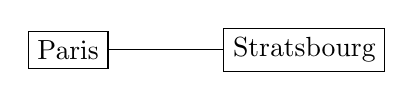
\begin{tikzpicture}
\node[draw] (S1) at (0,0) {Paris};
\node[draw] (S2) at (3,0) {Stratsbourg};
\draw (S1) -- (S2);
\end{tikzpicture}
\end{texexample}


The syntax of the command is:

|\node|\oarg{options} (\meta{name}) at (\meta{position}) |{|\meta{contents}|}|

If we look
 carefully, we see that the two writings give
Slightly different results:
- In the first case, node is an operation executed on a path. We
Can consider each node as a decoration of the point at which it
is associated. The line drawn by the draw command joins two points, the
Nodes are objects added later and centered on points. The option
Draw of the node trace operation the node outline.
- In the second case, \ node is a TikZ command which allows to define
A node, to name it and to draw it. One can then consider the
Nodes as pre-existing objects that will then be linked with the \docAuxCommand{node}.


\begin{texexample}{Draw a Line}{ex:line}
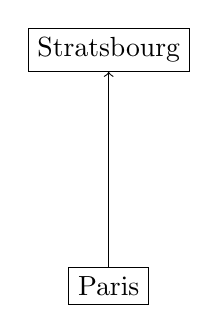
\begin{tikzpicture}
\node[draw] (S1) at (0,0) {Paris};
\node[draw] (S2) at (0,3) {Stratsbourg};
\draw[->] (S1) -- (S2);
\end{tikzpicture}
\end{texexample}

The basic building block of all pictures in \tikzname is the path. A path is a series of straight lines and curves
that are connected (that is not the whole picture, but let us ignore the complications for the moment). You
start a path by specifying the coordinates of the start position as a point in round brackets, as in (0,0).
This is followed by a series of \enquote{path extension operations.}


\begin{texexample}{Draw a Line}{ex:line}
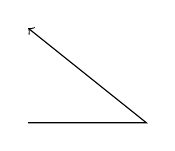
\begin{tikzpicture}
\draw[->] (0,0) -- (1.5,0) -- (0, 1.2);
\end{tikzpicture}
\end{texexample}


\subsection*{Adding Text} 

So far we have seen how to draw lines and arcs. However, an important component is still missing the addition of text. When
\tikzname is constructing a path and it encounters the keyword |node| typically followed by some options  it reads a \textit{node specification}. Options can typically follow and then it terminates by curly brackets. 
 

\begin{texexample}{Draw a Line}{ex:line}
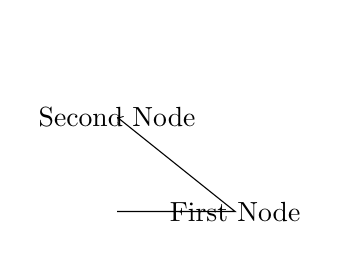
\begin{tikzpicture}
\draw[->] (0,0) -- (1.5,0) node {First Node} -- (0, 1.2) node[shape = circle] {Second Node};
\end{tikzpicture}
\end{texexample}


The \docAuxCommand*{node} can be used to abbreviate the operation. A longer example can demonstrate this better. How can we draw the following figure?

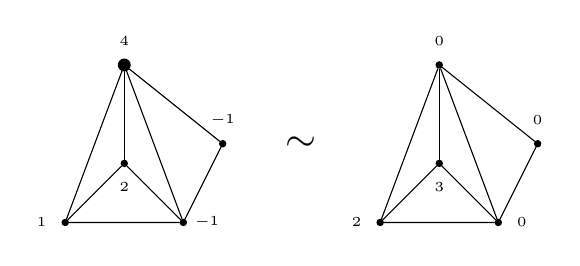
\begin{tikzpicture}
\node[circle,fill=black,inner sep=0.8pt,draw] (a) at (0,0) {};
\node[circle,fill=black,inner sep=0.8pt,draw] (b) at (1.5,0) {};
\node[circle,fill=black,inner sep=1.5pt,draw] (c) at (.75,2) {};
\node[circle,fill=black,inner sep=0.8pt,draw] (d) at (0.75,.75) {};
\node[circle,fill=black,inner sep=0.8pt,draw] (e) at (2,1) {};


\node () at (-0.3,0) {\tiny$1$};
\node () at (0.75,0.45) {\tiny$2$};
\node () at (0.75,2.3) {\tiny$4$};
\node () at (2,1.3) {\tiny$-1$};
\node () at (1.8,0) {\tiny$-1$};

\draw (a)--(b)--(e)--(c) --(a)--(d)--(b)--(c);
\draw (c)--(d);

\node at (3,1) {\Large{$\sim$}};

\begin{scope}[shift={(+4,0)}]
\node[circle,fill=black,inner sep=0.8pt,draw] (a) at (0,0) {};
\node[circle,fill=black,inner sep=0.8pt,draw] (b) at (1.5,0) {};
\node[circle,fill=black,inner sep=0.8pt,draw] (c) at (.75,2) {};
\node[circle,fill=black,inner sep=0.8pt,draw] (d) at (0.75,.75) {};
\node[circle,fill=black,inner sep=0.8pt,draw] (e) at (2,1) {};


\node () at (-0.3,0) {\tiny$2$};
\node () at (0.75,0.45) {\tiny$3$};
\node () at (0.75,2.3) {\tiny$0$};
\node () at (2,1.3) {\tiny$0$};
\node () at (1.8,0) {\tiny$0$};

\draw (a)--(b)--(e)--(c) --(a)--(d)--(b)--(c);
\draw (c)--(d);

\end{scope}
\end{tikzpicture}

\begin{texexample}{A larger example}{ex:larger}
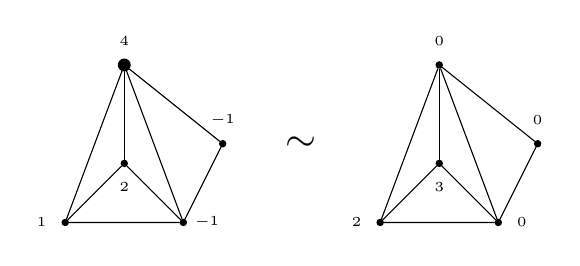
\begin{tikzpicture}
\node[circle,fill=black,inner sep=0.8pt,draw] (a) at (0,0) {};
\node[circle,fill=black,inner sep=0.8pt,draw] (b) at (1.5,0) {};
\node[circle,fill=black,inner sep=1.5pt,draw] (c) at (.75,2) {};
\node[circle,fill=black,inner sep=0.8pt,draw] (d) at (0.75,.75) {};
\node[circle,fill=black,inner sep=0.8pt,draw] (e) at (2,1) {};


\node () at (-0.3,0) {\tiny$1$};
\node () at (0.75,0.45) {\tiny$2$};
\node () at (0.75,2.3) {\tiny$4$};
\node () at (2,1.3) {\tiny$-1$};
\node () at (1.8,0) {\tiny$-1$};

\draw (a)--(b)--(e)--(c) --(a)--(d)--(b)--(c);
\draw (c)--(d);

\node at (3,1) {\Large{$\sim$}};

\begin{scope}[shift={(+4,0)}]
\node[circle,fill=black,inner sep=0.8pt,draw] (a) at (0,0) {};
\node[circle,fill=black,inner sep=0.8pt,draw] (b) at (1.5,0) {};
\node[circle,fill=black,inner sep=0.8pt,draw] (c) at (.75,2) {};
\node[circle,fill=black,inner sep=0.8pt,draw] (d) at (0.75,.75) {};
\node[circle,fill=black,inner sep=0.8pt,draw] (e) at (2,1) {};


\node () at (-0.3,0) {\tiny$2$};
\node () at (0.75,0.45) {\tiny$3$};
\node () at (0.75,2.3) {\tiny$0$};
\node () at (2,1.3) {\tiny$0$};
\node () at (1.8,0) {\tiny$0$};

\draw (a)--(b)--(e)--(c) --(a)--(d)--(b)--(c);
\draw (c)--(d);

\end{scope}
\end{tikzpicture}
\captionof{figure}{The larger vertex fires once to move from the left configuration to the right configuration.}
\end{texexample}

Behind the scenes pgf uses the basic system command \docAuxCommand{pgfnode} to create the nodes. The syntax of the command is given on \seepgfmanual{1026} as:

\begin{docCommand}{pgfnode}{\marg{shape}\marg{anchor}\marg{label text}\marg{name}\marg{path usage command}}
This command creates a new node. The \marg{shape} of the node must have been declared previously using
\lstinline{pgfdeclareshape}.

The shape is shifted such that the \marg{anchor} is at the origin. In order to place the shape somewhere else,
use the coordinate transformation prior to calling this command.
The hnamei is a name for later reference. If no name is given, nothing will be “saved” for the node, it
will just be drawn.

The \marg{path usage command} is executed for the background and the foreground path (if the shape defines
them).
\end{docCommand}


A good workflow, is to first define the nodes, next label them and then draw any connecting lines.

\begin{texexample}{Named nodes}{ex:named} 
\begin{tikzpicture}
\node[circle,fill=black,inner sep=0.8pt,draw] (a) at (0,0) {};
\node[circle,fill=black,inner sep=0.8pt,draw] (b) at (1.5,0) {};
\node[circle,fill=black,inner sep=1.5pt,draw] (c) at (.75,2) {};
\node[circle,fill=black,inner sep=0.8pt,draw] (d) at (0.75,.75) {};
\node[circle,fill=black,inner sep=0.8pt,draw] (e) at (2,1) {};
\end{tikzpicture}
\end{texexample}

\begin{texexample}{Named nodes}{ex:named} 
\begin{tikzpicture}
\node[circle,fill=black,inner sep=0.8pt,draw] (a) at (0,0) {};
\node[circle,fill=black,inner sep=0.8pt,draw] (b) at (1.5,0) {};
\node[circle,fill=black,inner sep=1.5pt,draw] (c) at (.75,2) {};
\node[circle,fill=black,inner sep=0.8pt,draw] (d) at (0.75,.75) {};
\node[circle,fill=black,inner sep=0.8pt,draw] (e) at (2,1) {};
% absolute labelling
\node () at (-0.3,0) {\tiny$1$};
\node () at (0.75,0.45) {\tiny$2$};
\node () at (0.75,2.3) {\tiny$4$};
\node () at (2,1.3) {\tiny$-1$};
\node () at (1.8,0) {\tiny$-1$};
\end{tikzpicture}
\end{texexample}

\begin{texexample}{Named nodes}{ex:named} 
\begin{tikzpicture}
\pgfdeclarelayer{background}
\pgfdeclarelayer{foreground}
\pgfsetlayers{background,main,foreground}
\node[circle,fill=black,inner sep=0.8pt,draw] (a) at (0,0) {};
\node[circle,fill=black,inner sep=0.8pt,draw] (b) at (1.5,0) {};
\node[circle,fill=black,inner sep=1.5pt,draw] (c) at (.75,2) {};
\node[circle,fill=black,inner sep=0.8pt,draw] (d) at (0.75,.75) {};
\node[circle,fill=black,inner sep=0.8pt,draw] (e) at (2,1) {};
% absolute labelling
\node () at (-0.3,0) {\tiny$1$};
\node () at (0.75,0.45) {\tiny$2$};
\node () at (0.75,2.3) {\tiny$4$};
\node () at (2,1.3) {\tiny$-1$};
\node () at (1.8,0) {\tiny$-1$};
% draw connecting lines
\draw (a)--(b)--(e)--(c) --(a)--(d)--(b)--(c);
\draw (c)--(d);
%\begin{pgfonlayer}{background}
\begin{scope}[on background layer={color=blue!10}]
\node [fill=blue!10,fit=(a) (b) (c)
(d) (e)] {};
\end{scope}
%\end{pgfonlayer}
\end{tikzpicture}
\end{texexample}

Just to recap, using \docAuxCommand*{node} and the \textbf{at} we can position accurately any node. We could have used the much longer command |path node|, but in our case above this is unecessary (\seepgfmanual{49}), for more explanations if you are still unsure.

Nodes can be named or unnamed. There are two ways to name them, with the key \docValue{name} or within brackets. The second method is to be preferred. Names for nodes can be pretty arbitrary, but they should not contain commas, periods, parentheses, colons, and some other special characters. However, they can contain underscores and hyphens

\subsection{Layers and Scope}

We can add a backround layer, using the library \textit{backgrounds}, which provides key values for adding backgrounds. \pgfname\ provides a layering mechanism for composing graphics from
multiple layers. (This mechanism is not to be confused with the
conceptual ``software layers'' the \pgfname\ system is composed of.)
Layers are often used in graphic programs. The idea is that you can
draw on the different layers in any order. So you might start drawing
something on the ``background'' layer, then something on the
``foreground'' layer, then something on the ``middle'' layer, and then
something on the background layer once more, and so on. At the end, no
matter in which ordering you drew on the different layers, the layers
are ``stacked on top of each other'' in a fixed ordering to produce
the final picture. Thus, anything drawn on the middle layer would come
on top of everything of the background layer.

Normally, you do not need to use different layers since you will have
little trouble ``ordering'' your graphic commands in such a way that
layers are superfluous. However, in certain situations you only
``know'' what you should draw behind something else after the
``something else'' has been drawn.

For example, suppose you wish to draw a yellow background behind your
picture. The background should be as large as the bounding box of the
picture, plus a little border. If you know the size of the bounding box
of the picture at its beginning, this is easy to accomplish. However,
in general this is not the case and you need to create a
``background'' layer in addition to the standard ``main'' layer. Then,
at the end of the picture, when the bounding box has been established,
you can add a rectangle of the appropriate size to the picture.

\subsection{Declaring Layers}

In \pgfname\ layers are referenced using names. The standard layer,
which is a bit special in certain ways, is called |main|. If nothing
else is specified, all graphic commands are added to the |main|
layer. You can declare a new layer using the following command:

\begin{docCommand}{pgfdeclarelayer}{\marg{name}}
  This command declares a layer named \meta{name} for later
  use. Mainly, this will set up some internal bookkeeping.
\end{docCommand}

The next step toward using a layer is to tell \pgfname\ which layers
will be part of the actual picture and which will be their
ordering. Thus, it is possible to have more layers declared than are
actually used.

\begin{docCommand}{pgfsetlayers}{\marg{layer list}}
  This command tells \pgfname\ which layers will be used in
  pictures. They are stacked on top of each other in the order
  given. The layer |main| should always be part of the list. Here is
  an example:
\begin{codeexample}[code only]
\pgfdeclarelayer{background}
\pgfdeclarelayer{foreground}  
\pgfsetlayers{background,main,foreground}
\end{codeexample}

  This command should be given either outside of any picture or ``directly inside'' of a picture.
  Here, the ``directly inside'' means that there should be no further level of \TeX\ grouping between |\pgfsetlayers| and the matching |\end{pgfpicture}| (no closing braces, no |\end{...}|). It will also work if |\pgfsetlayers| is provided before |\end{tikzpicture}| (with similar restrictions).
\end{docCommand}


\subsection{Using Layers}

Once the layers of your picture have been declared, you can start to
``fill'' them. As said before, all graphics commands are normally
added to the |main| layer. Using the |{pgfonlayer}| environment, you
can tell \pgfname\ that certain commands should, instead, be added to
the given layer.

\begin{docEnvironment}{pgfonlayer}{\marg{layer name}}
\end{docEnvironment}

The whole \meta{environment contents} is added to the layer with the
name \meta{layer name}. This environment can be used anywhere inside
a picture. Thus, even if it is used inside a |{pgfscope}| or a \TeX\
group, the contents will still be added to the ``whole'' picture.
Using this environment multiple times inside the same picture will
cause the \meta{environment contents} to accumulate.

  \emph{Note:} You can \emph{not} add anything to the |main| layer
  using this environment. The only way to add anything to the main
  layer is to give graphic commands outside all |{pgfonlayer}|
  environments. 



\begin{codeexample}[]
\pgfdeclarelayer{background layer}
\pgfdeclarelayer{foreground layer}
\pgfsetlayers{background layer,main,foreground layer}
\begin{tikzpicture}
  % On main layer:
  \fill[blue] (0,0) circle (1cm);
  
  \begin{pgfonlayer}{background layer}
    \fill[yellow] (-1,-1) rectangle (1,1);
  \end{pgfonlayer}
  
  \begin{pgfonlayer}{foreground layer}
    \node[white] {foreground};
  \end{pgfonlayer}
  
  \begin{pgfonlayer}{background layer}
    \fill[black] (-.8,-.8) rectangle (.8,.8);
  \end{pgfonlayer}

  % On main layer again:
  \fill[blue!50] (-.5,-1) rectangle (.5,1);
\end{tikzpicture}
\end{codeexample}



\long\gdef\mytriangle{
\node[circle,fill=black,inner sep=0.8pt,draw] (a) at (0,0) {};
\node[circle,fill=black,inner sep=0.8pt,draw] (b) at (1.5,0) {};
\node[circle,fill=black,inner sep=1.5pt,draw] (c) at (.75,2) {};
\node[circle,fill=black,inner sep=0.8pt,draw] (d) at (0.75,.75) {};
\node[circle,fill=black,inner sep=0.8pt,draw] (e) at (2,1) {};
% absolute labelling
\node () at (-0.3,0) {\tiny$1$};
\node () at (0.75,0.45) {\tiny$2$};
\node () at (0.75,2.3) {\tiny$4$};
\node () at (2,1.3) {\tiny$-1$};
\node () at (1.8,0) {\tiny$-1$};
% draw connecting lines
\draw (a)--(b)--(e)--(c) --(a)--(d)--(b)--(c);
\draw (c)--(d);
}

\begin{texexample}{Adding backgrouns}{ex:backgrounds}
\begin{tikzpicture}
\pgfdeclarelayer{background}
\pgfdeclarelayer{foreground}
\pgfsetlayers{background,main,foreground}
\mytriangle
%\begin{pgfonlayer}{background}
\begin{scope}[on background layer={color=blue!10}]
\mytriangle
\node [fill=blue!10,fit=(a) (b) (c)
(d) (e)] {};
\end{scope}
%\end{pgfonlayer}
\end{tikzpicture}
\end{texexample}


\begin{texexample}{Adding backgrouns}{ex:backgrounds}
\begin{tikzpicture}
\pgfdeclarelayer{background}
\pgfdeclarelayer{foreground}
\pgfsetlayers{background,main,foreground}
\mytriangle
%\begin{pgfonlayer}{background}
\begin{scope}[on background layer={color=blue!10}]
\node [fill=blue!10,fit=(a) (b) (c)
(d) (e)] {};
\end{scope}

\begin{scope}[shift={(+4,0)}]
\mytriangle
\begin{pgfonlayer}{background}
\node [pattern=checkerboard light gray,fit=(a) (b) (c)
(d) (e)] {};
\end{pgfonlayer}
\end{scope}
\end{tikzpicture}
\end{texexample}

This brings us to the end of our discussion. Time for a coffee and a break.                

\section{Adding styles}

In our previous example, we cut and pasted many of the repetitive keys. \pgfname offers a way to set a new key to the values of other keys using the handler |.style|. This is a very powerful way of redefining new keys, but also simplifying the code. Styles in \tikzname can be considered similar to macros in standard LaTeX. When I made a drawing, we can still tweak the styles and look how the drawing changes, until it's perfect. You should never have to tweak each node.

\begin{texexample}{Using styles}{ex:usingstyles}
\tikzset{BN/.style = {circle,fill=black,inner sep=0.8pt,draw},
         tiny/.style = {font=\tiny}, 
}
\begin{tikzpicture}
\node[BN] (a) at (0,0) {};
\node[BN] (b) at (1,0) {};
\node[BN] (c) at (1,1) {};
\node[BN] (d) at (0,1) {};
\node[BN] (e) at (-1,0) {};

\node () at (-1.3,0) [tiny]{$v_1$};
\node () at (-.3,1)  [tiny]{$v_2$};
\node () at (1.3,0)  [tiny]{$w_1$};
\node () at (1.3,1)  [tiny]{$w_2$};

\node[tiny] () at (0.5,-0.2) {$a$};
\node[tiny] () at (0.5,1.2) {$b$};
\node[tiny] () at (0.2,0.5) {$c$};
\node[tiny] () at (-0.5,-.2) {$d$};

\draw (e) -- (a) -- (b) -- (c) -- (d) -- (a);
\draw (e) -- (d);

\end{tikzpicture}
\end{texexample}



\section{Arcs and options for lines}

\begin{texexample}{Draw a Line}{ex:line}
\begin{tikzpicture}
\draw[->] (0,0) -- (1.5,0) node[draw, ellipse] {First Node} -| (0, 1.2) node[draw,ellipse,rotate=45] {Second Node};
\end{tikzpicture}
\end{texexample}

\begin{texexample}{Drawing arcs}{ex:matharcs}
We define 
\begin{gather*}
    \bar{d}_{k,l}:=\hspace{6pt}
    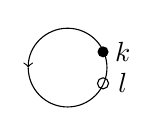
\begin{tikzpicture}[baseline=(current bounding box.center)]
    \draw[->] (3,2) arc (-180:180:5mm);
	  \fill (3.95,2.2) circle [radius=2pt];
    \draw (3.95,1.8) circle [radius=2pt];
    \node at (4.2,1.8) {$l$};
    \node at (4.2,2.2) {$k$};
    \end{tikzpicture}
    \hspace{0.5cm}
    \text{and}
    \hspace{0.5cm}
    d_{k,l}:=\hspace{6pt}
    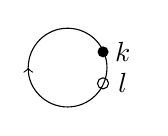
\begin{tikzpicture}[baseline=(current bounding box.center)]
    \draw[<-] (3,2) arc (-180:180:5mm);
    \fill (3.95,2.2) circle [radius=2pt];
    \draw (3.95,1.8) circle [radius=2pt];
    \node at (4.2,1.8) {$l$};
    \node at (4.2,2.2) {$k$};
    \end{tikzpicture}
    \hspace{0.5cm}
    \text{for}
    \hspace{2mm} k,l\in\mathbb{Z}_{\geq 0}.
\end{gather*}
\end{texexample}


Here is a figure that you should try and reproduce.
\newcommand{\G}{\Gamma}

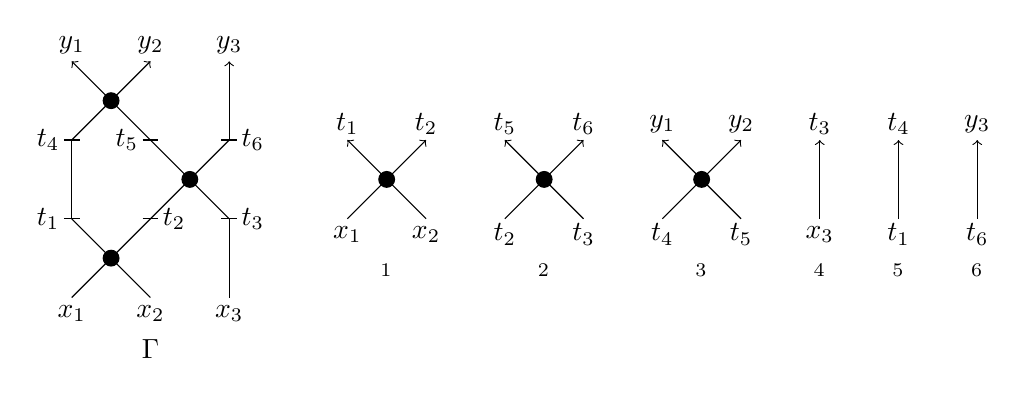
\begin{tikzpicture}
\draw (-3.5,-1)--(-2.5,0); \draw (-2.5,-1)--(-3.5,0); \draw (-1.5,-1)--(-1.5,0);\draw[fill=black] (-3,-0.5) circle (0.1cm); \draw (-3.5,0)--(-3.5,1); \draw (-2.5,0)--(-1.5,1); \draw (-1.5,0)--(-2.5,1);\draw[fill=black] (-2,0.5) circle (0.1cm); \draw[->] (-3.5,1)--(-2.5,2); \draw[->] (-2.5,1)--(-3.5,2); \draw[->] (-1.5,1)--(-1.5,2); \draw[fill=black] (-3,1.5) circle (0.1cm); \draw (-3.6,0)--(-3.4,0);\draw (-2.6,0)--(-2.4,0);\draw (-1.6,0)--(-1.4,0); \draw (-3.6,1)--(-3.4,1);\draw (-2.6,1)--(-2.4,1);\draw (-1.6,1)--(-1.4,1); \node at (-3.5,-1.2) {$x_1$};\node at (-2.5,-1.2) {$x_2$};\node at (-1.5,-1.2) {$x_3$}; \node at (-3.5,2.2) {$y_1$};\node at (-2.5,2.2) {$y_2$};\node at (-1.5,2.2) {$y_3$}; \node at (-3.8,0) {$t_1$};\node at (-2.2,0) {$t_2$};\node at (-1.2,0) {$t_3$}; \node at (-3.8,1) {$t_4$};\node at (-2.8,1) {$t_5$};\node at (-1.2,1) {$t_6$}; \node at (-2.5,-1.65) {$\Gamma$};
\draw[->] (0,0)--(1,1); \draw[->] (1,0)--(0,1); \draw[fill=black] (0.5,0.5) circle (0.1cm); \draw[->] (2,0)--(3,1); \draw[->] (3,0)--(2,1); \draw[fill=black] (2.5,0.5) circle (0.1cm); \draw[->] (4,0)--(5,1); \draw[->] (5,0)--(4,1); \draw[fill=black] (4.5,0.5) circle (0.1cm); \draw[->] (6,0)--(6,1); \draw[->] (7,0)--(7,1); \draw[->] (8,0)--(8,1);
\node at (0,-.2) {$x_1$};\node at (1,-.2) {$x_2$}; \node at (2,-.2) {$t_2$};\node at (3,-.2) {$t_3$}; \node at (4,-.2) {$t_4$};\node at (5,-.2) {$t_5$}; \node at (6,-.2) {$x_3$}; \node at (7,-.2) {$t_1$}; \node at (8,-.2) {$t_6$};
\node at (0,1.2) {$t_1$};\node at (1,1.2) {$t_2$}; \node at (2,1.2) {$t_5$};\node at (3,1.2) {$t_6$}; \node at (4,1.2) {$y_1$};\node at (5,1.2) {$y_2$}; \node at (6,1.2) {$t_3$}; \node at (7,1.2) {$t_4$}; \node at (8,1.2) {$y_3$};
\node at (0.5,-0.65) {$\G_1$}; \node at (2.5,-0.65) {$\G_2$}; \node at (4.5,-0.65) {$\G_3$}; \node at (6,-0.65) {$\G_4$};\node at (7,-0.65) {$\G_5$};\node at (8,-0.65) {$\G_6$}; 
\end{tikzpicture}

This brings us to the end.




The |node| can take numerous options who are then used to set the typesetting of the text that follows:


\begin{texexample}{Draw a Line}{ex:line}
\begin{tikzpicture}
\draw[->] (0,0) -- (1.5,0) node[draw, ellipse] {First Node} -| (0, 1.2) node[draw,ellipse,rotate=45, text width=3cm, fill=creamy, text justified] {\lorem};
\end{tikzpicture}
\end{texexample}


\begin{texexample}{Draw a Line}{ex:line}
\begin{tikzpicture}[funny ellipse/.style = {draw,ellipse,rotate=45, text width=3cm, fill=creamy, text justified} ]
\draw[->] (0,0) -- (1.5,0) node[draw, ellipse] {First Node} -| (0, 1.2) node[funny ellipse] {\lorem};
\end{tikzpicture}
\end{texexample}

This can also be written by using \docAuxCommand{tikzset} for setting out all the keys. This can written just before the environment or within the scope of the environment. See \href{https://tex.stackexchange.com/questions/52372/should-tikzset-or-tikzstyle-be-used-to-define-tikz-styles}{TX.SX discussion}, for the option to set |\tikzstyle| which should not be used, even if it is quicker to write.


\begin{texexample}{Draw a Line}{ex:line}
\tikzset{funny ellipse/.style = {draw,ellipse,rotate=45, text width=3cm, fill=creamy, text justified} }
\begin{tikzpicture}
\draw[->] (0,0) -- (1.5,0) node[draw, ellipse] {First Node} -| (0, 1.2) node[funny ellipse] {\lorem};
\end{tikzpicture}
\end{texexample}

A |node| can possibly be rendered with a choice from a list of over 720 keys.

ed. 



Using the |TikZ| package you can draw figures and intermingle them with text. To draw a simple diamond as shown in \fref{fig:diamond} we use
the following commands. The package comes with a very comprehensive manual of over 500 pages long. One can state that there is nothing that you cannot draw with PGF/TikZ, if you have the patience and perseverance. TikZ's language has a syntax of its own with very little connection to what we have used so far. You will need to set aside adequate time to study this, especially if your work has a lot of specially drawn figures that you need. The result like anything else in \tex make the effort worthwhile.

\begin{texexample}{Draw a Diamond}{fig:diamond}

\begin{tikzpicture}
 \draw (1,0) -- (0,1) -- (-1,0) -- (0,-1) -- cycle;
\end{tikzpicture}
\end{texexample}


\begin{texexample}{Text long path}{ex:decorations}
\begin{tikzpicture}
\draw [help lines] grid (3,2);
\draw [red, dashed]
[postaction={decoration={text along path, text={a big juicy apple},
text align=fit to path}, decorate}]
(0,0) .. controls (0,2) and (3,2) .. (3,0);
\node (A) at (1.5,0) {!};
\end{tikzpicture}
\end{texexample}


\begin{texexample}{Text long path}{ex:decorations}

Hello \begin{pgfpicture}
\pgfpathrectangle{\pgfpointorigin}{\pgfpoint{2ex}{1ex}}
\pgfusepath{stroke}
\end{pgfpicture} World!

\end{texexample}


\emphasis{-,draw,begin,end,tikzpicture}
\begin{teXXX}

\begin{tikzpicture}
\draw (1,0) -- (0,1) -- (-1,0) -- (0,-1) -- cycle;
\end{tikzpicture}
\end{teXXX}



\makeatletter
The value of $x$ is \pgfsys@markposition{here}important.

Lots of text.
\hbox{\pgfsys@markposition{myorigin}%
\begin{pgfpicture}
% Switch of size protocol
\pgfpathmoveto{\pgfpointorigin}
\pgfusepath{use as bounding box}
\pgfsys@getposition{here}{\hereposition}
\pgfsys@getposition{myorigin}{\thispictureposition}
\pgftransformshift{\pgfpointscale{-1}{\thispictureposition}}
\pgftransformshift{\hereposition}
\pgfpathcircle{\pgfpointorigin}{1cm}
\pgfusepath{draw}
\end{pgfpicture}}

\makeatother


You cannot write directly into a picture environment. The command \docAuxCommand{pgftext} can be used. 

\begin{texexample}{Using text directly}{ex:pgftext}
\tikz{\draw[help lines] (0,0) grid (3,2);
\pgftext[base,x=1cm,y=0.5cm] {lovely}}
\end{texexample}





Sometimes it is quite useful when debugging to add a backround grid. 


\begin{centering}
\begin{tikzpicture}
\draw[step=0.25cm,color=creamy] (-1,-1) grid (1,1);
\draw [color=bgsexy](1,0) -- (0,1) -- (-1,0) -- (0,-1) -- cycle;
\end{tikzpicture}
\captionof{figure}{You can add a background grid using \texttt{step=0.25cm, color=green} as an option}
\end{centering}


\emphasis{step,color,green,grid,begin,end}
\begin{teXXX}
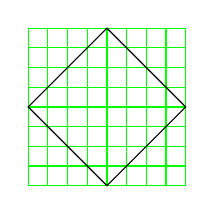
\begin{tikzpicture}
  \draw[step=0.25cm,color=green] (-1,-1) grid (1,1);
  \draw (1,0) -- (0,1) -- (-1,0) -- (0,-1) -- cycle;
\end{tikzpicture}
\end{teXXX}

The grid is specified by providing two diagonally opposing points: (-1,-1)
and (1, 1). The two options supplied give a step size for the grid lines and a
specification for the color of the grid lines, using the \docpkg{xcolor} package

\subsection{Specifying points and paths}

\begin{texexample}{Specifying points and paths}{ex:points}
\centering
\begin{tikzpicture}[scale=1.8]
% Define the points of a regular pentagon
\path (0,0) coordinate (origin);
\path (0:1cm) coordinate (P0);
\path (1*72:1cm) coordinate (P1);
\path (2*72:1cm) coordinate (P2);
\path (3*72:1cm) coordinate (P3);
\path (4*72:1cm) coordinate (P4);
% Draw the edges of the pentagon
\draw[color=bgsexy] (P0) -- (P1) -- (P2) -- (P3) -- (P4) -- cycle;
% Add "spokes"
\draw[color=bgsexy] (origin) -- (P0) (origin) -- (P1) (origin) -- (P2)
(origin) -- (P3) (origin) -- (P4);
\end{tikzpicture}
\captionof{figure}{Drawing a complicated polygon, using paths and the \texttt{draw} command}
\end{texexample}


Two key ideas used in \tikzname\ are points and paths. Both of these ideas were used
in the diamond examples. Much more is possible, however. For example, points
can be specified in any of the following ways:
\begin{enumerate}
\item  Cartesian coordinates
\item  Polar coordinates
\item  Named points
\item  Relative points
\end{enumerate}



\subsection{coordinates}
The cartesian coordinates can be defined and named using the following syntax.

%\emphasis{begin,end,coordinate,at,draw}
%\begin{teXXX}
%\begin{tikzpicture}
%  \coordinate (A) at (0,0);
%  \coordinate (B) at (1.25,0.25);
%  \draw[blue] (A) -- (B);
%\end{tikzpicture}
%\end{teXXX}

\noindent This produces:
\begin{tikzpicture}
\coordinate (A) at (0,0);
\coordinate (B) at (1.25,0.25);
\draw[blue] (A) -- (B);
\end{tikzpicture}


We can add labels to the points by using the |label| option. A label is distinct from the text of a |node|.

\begin{tikzpicture}
\coordinate [label=left:\textcolor{orange}{$A$}] (A) at (0,0);
\coordinate [label=right:\textcolor{orange}{$B$}]  (B) at (1.15,0.25);
\draw[blue] (A) -- (B);
\end{tikzpicture}

\emphasis{label,left,label:,right}
\begin{teXXX}
\begin{tikzpicture}
  \coordinate [label=left:\textcolor{orange}{$A$}] (A) at (0,0);
  \coordinate [label=west:\textcolor{orange}{$B$}] (B) at (1.25,0.25);
  \draw[blue] (A) -- (B);
\end{tikzpicture}
\end{teXXX}




If you tempted to write \texttt{label=top:} it will not work, as the command accepts the following keywords.


\begin{tikzpicture}
  \coordinate [label=left:\textcolor{orange}{east}]  (A) at (0,0);
  \coordinate [label=right:\textcolor{orange}{west}] (B) at (0,0);
  \draw[blue] (A)--(B);
\end{tikzpicture}


\section{Graphic Parameters: Line Width, Line Cap, and Line Join}

The width of lines can be specified using the key:

\begin{docKey}[tikz]{line width}{=\marg{dimension}} {no default, initially 0.4pt}
Specifies the line width \seepgfmanual{166}
\end{docKey}



\bgroup
\def\mkl#1{\tikz \draw[#1] (0,0)--(1.0, 1.5ex);}
\scriptsize\arial
\begin{tabular}{|l|l|l|l|l|l|l|l|}
\hline
\mkl{line width=2pt}& \mkl{ultra thin} &\mkl{very thin} & \mkl{thin} & \mkl{semithick} & \mkl{thick} &\mkl{very thick} &\mkl{ultra thick} \\
\hline
line width=2pt &ultra thin & very thin & thin &semithick & thick & very thick & ultra thick \\
\hline
\end{tabular}
\egroup

\begin{docKey}[tikz]{line cap}{=\marg{dimension}} {no default, initially 0.4pt}
Specifies how lines “end.” Permissible types are round, rect, and butt \seepgfmanual{167}. 
\end{docKey}

\bgroup
\def\mkl#1{\begin{tikzpicture} \draw[line width=10pt, line cap=#1] (0,0)--(1.0, 1.5ex);\draw[white,line width=2pt]
(0,0 )--(1.0,1.5ex);\end{tikzpicture}}
\scriptsize\arial
\begin{tabular}{|l|l|l|}
\hline
\mkl{rect}& \mkl{butt} &\mkl{round}  \\
\hline
rect &butt & round \\
\hline
\end{tabular}
\egroup




\begin{docKey}[tikz]{line join}{=\marg{type}}{no default, initially miter}
Specifies how lines “join.” Permissible type are round, bevel, and miter. They have the following
effects:
\end{docKey}

\begin{texexample}{Joining Lines}{es:joinlines}

\begin{tikzpicture}[line width=10pt]
\draw[line join=round] (0,0) -- ++(.5,1) -- ++(.5,-1);
\draw[line join=bevel] (1.25,0) -- ++(.5,1) -- ++(.5,-1);
\draw[line join=miter] (2.5,0) -- ++(.5,1) -- ++(.5,-1);
\end{tikzpicture}
\end{texexample}


\begin{docKey}[tikz]{dash pattern}{=\marg{dash pattern}}{no default}
Sets the dashing pattern. The syntax is the same as in \metafontlogo. For example following pattern on
2pt off 3pt on 4pt off 4pt means \enquote{draw 2pt, then leave out 3pt, then draw 4pt once more, then
leave out 4pt again, repeat}.
\end{docKey}

\bgroup
\def\ml#1{\tikz \draw[ #1] (0pt,0pt) -- (50pt,0pt);}
\def\alist{solid, dotted, densely dotted, loosely dotted,% 
           dashed,densely dashed, loosely dashed, %
           dash dot, densely dash dot, loosely dash dot, %
           dash dot dot, densely dash dot dot, loosely dash dot dot.}

For patterns there are numerous settings {\arial \alist }


\scriptsize
\begin{tabular}{lll}
\hline
\ml{solid} &  & \\
solid      &  & \\
\hline
\ml{dotted} &\ml{densely dotted} & \ml{loosely dotted}\\
\textit{dotted} & densely dotted  &loosely dotted \\
\hline
\ml{dashed} & \ml{densely dashed} & \ml{loosely dashed}  \\
\textit{dashed}      & densely dashed & loosely dashed            \\
\hline

\ml{dash dot} & \ml{densely dash dot} & \ml{loosely dash dot} \\
\textit{dash dot} & densely dash dot & loosely dash dot \\
\hline

\ml{dash dot dot} & \ml{densely dash dot dot} & \ml{loosely dash dot dot} \\
\textit{dash dot dot} & densely dash dot dot & loosely dash dot dot \\
\hline
\end{tabular}
\egroup


\subsection{Pattern Library}

The library patterns can be used to draw predetermined patterns. This will be a longer than usual section as it explains how to create new patterns. Most of the content is straight from the \pgfname manual. Before we start with the creation f a new pattern let us examine how a pattern is used.

\begin{texexample}{Using Library Patterns}{ex:libpatterns}
\begin{tikzpicture}
\pattern [path fading=west,pattern=checkerboard light gray]
      (0,0) rectangle (5cm,2em);
\end{tikzpicture}
\end{texexample}


\label{section-library-patterns}


The package defines patterns for filling areas. \docAuxCommand*{usetikzlibrary}\marg{patterns}.




\subsection{Form-Only Patterns}

\begin{tabular}{ll}
  \emph{Pattern name} & \emph{Example (pattern in black, blue, and red
    on faded checkerboard)} \\ 
  \patternindex{horizontal lines} 
  \patternindex{vertical lines} 
  \patternindex{north east lines} 
  \patternindex{north west lines} 
  \patternindex{grid} 
  \patternindex{crosshatch} 
  \patternindex{dots} 
  \patternindex{crosshatch dots} 
  \patternindex{fivepointed stars} 
  \patternindex{sixpointed stars} 
  \patternindex{bricks}
  \patternindex{checkerboard}
\end{tabular}
  
\subsection{Inherently Colored Patterns}


\begin{tabular}{ll}
  \emph{Pattern name} & \emph{Example} \\
  \patternindexinherentlycolored{checkerboard light gray} 
  \patternindexinherentlycolored{horizontal lines light gray} 
  \patternindexinherentlycolored{horizontal lines gray} 
  \patternindexinherentlycolored{horizontal lines dark gray} 
  \patternindexinherentlycolored{horizontal lines light blue} 
  \patternindexinherentlycolored{horizontal lines dark blue} 
  \patternindexinherentlycolored{crosshatch dots gray} 
  \patternindexinherentlycolored{crosshatch dots light steel blue} 
\end{tabular}
  


% Copyright 2006 by Till Tantau
%
% This file may be distributed and/or modified
%
% 1. under the LaTeX Project Public License and/or
% 2. under the GNU Free Documentation License.
%
% See the file doc/generic/pgf/licenses/LICENSE for more details.


\section{Creating Patterns}

\label{section-patterns}

\subsection{Overview}

There are many ways of filling a path. First, you can fill it using a
solid color and this is also the fastest method. Second, you can also
fill it using a shading, which means that the color changes smoothly
between two (or more) different colors. Third, you can fill it using a
tiling pattern and it is explained in the following how this is done.

A tiling pattern can be imagined as a rectangular tile (hence the
name) on which a small picture is painted. There is not a single tile,
but (conceptually) an infinite number of tiles, all showing the same
picture, and these tiles are arranged horizontally and vertically to
fill the plane. When you use a tiling pattern to fill a path, what
happens is that the path clips out a ``window'' through which we see
part of this infinite plane.

Patterns come in two versions: \emph{inherently colored patterns} and
\emph{form-only patterns}. (These are often called ``color patterns''
and ``uncolored patterns,'' but these names are misleading since
uncolored patterns do have a color and the color changes. As I said,
the name is misleading\dots) An inherently colored pattern is just a
colored tile like, say, a red star with a black outline. A form-only
pattern can be imagined as a tile that is a kind of rubber stamp. When
this pattern is used, the stamp is used to print copies of the stamp
picture onto the plane, but we can use a different stamp color each
time we use a form-only pattern.

\pgfname\ provides a special support for patterns. You can declare a
pattern and then use it very much like a fill color. \pgfname\
directly maps patterns to the pattern facilities of the underlying
graphic languages (PostScript, \textsc{pdf}, and \textsc{svg}). This
means that filling a path using a pattern will be nearly as fast as if
you used a uniform color.

There are a number of pitfalls and restrictions when using
patterns. First, once a pattern has been declared, you cannot change
it anymore. In particular, it is not possible to enlarge it or change
the line width. Such flexibility would require that the repeating of
the pattern were not done by the graphic language, but on the
\pgfname\ level. This would make patterns orders of magnitude slower
to produce and to render. However, \pgfname{} does provide a
more-or-less successful emulation of ``mutable'' patterns, although
internally, a new (fixed) instance of a pattern is declared when
the parameters of a pattern change.

Second, the phase of patterns is not well-defined, that is, it is not
clear where the origin of the ``first'' tile is. To be more precise,
PostScript and \textsc{pdf} on the one hand and \textsc{svg} on the
other hand define the origin differently. PostScript and \textsc{pdf}
define a fixed origin that is independent of where the path lies. This
has the highly desirable effect that if you use the same pattern to
fill multiple paths, the outcome is the same as if you had filled a 
single path consisting of the union of all these paths. By
comparison, \textsc{svg} uses the upper-left (?) corner of the path to
be filled as the origin. However, the \textsc{svg} specification is a
bit vague on this question.


\subsection{Declaring a Pattern}

Before a pattern can be used, it must be declared. The following
command is used for this:

\begin{docCommand}{pgfdeclarepatternformonly}{%
	\oarg{variables}%
	\marg{name}%
	\marg{bottom left}%
	\marg{top right}%
	\marg{tile size}%
	\marg{code}}

	This command declares a new form-only pattern. The \meta{name} is a
  name for later reference. The two parameters \meta{lower left} and
  \meta{upper right} must describe a bounding box that is large enough
  to encompass the complete tile.
\end{docCommand}

  The size of a tile is given by \meta{tile size}, that is, a tile is
  a rectangle whose lower left   corner is the origin and whose upper
  right corner is given by \meta{tile size}. This might make you
  wonder why the second and third parameters are needed. First, the
  bounding box might be smaller than the tile size if the tile is
  larger than the picture on the tile. Second, the bounding box might
  be bigger, in which case the picture will ``bleed'' over the tile.

  The \meta{code} should be \pgfname\ code than can be protocolled. It
  should not contain any color code.


\begin{codeexample}[]
\pgfdeclarepatternformonly{stars}
{\pgfpointorigin}{\pgfpoint{1cm}{1cm}}
{\pgfpoint{1cm}{1cm}}
{
  \pgftransformshift{\pgfpoint{.5cm}{.5cm}}
  \pgfpathmoveto{\pgfpointpolar{0}{4mm}}
  \pgfpathlineto{\pgfpointpolar{144}{4mm}}
  \pgfpathlineto{\pgfpointpolar{288}{4mm}}
  \pgfpathlineto{\pgfpointpolar{72}{4mm}}
  \pgfpathlineto{\pgfpointpolar{216}{4mm}}
  \pgfpathclose%
  \pgfusepath{fill}
}
\begin{tikzpicture}
  \filldraw[pattern=stars] (0,0)   rectangle (1.5,2);
  \filldraw[pattern=stars,pattern color=red]
                           (1.5,0) rectangle (3,2);
\end{tikzpicture}
\end{codeexample}

	The optional argument \meta{variables} consists of a comma
	separated	list of macros,	registers or keys, representing the
	parameters of the pattern that may vary. If a variable is a key,
	then the full path name must be used (specifically, it must start
	with |/|).
	As an example, a list might look like the following:
	|\mymacro,\mydimen,/pgf/my key|. Note that macros and keys should
	be ``simple''. They should only store values in themselves.
	
	The effect of \meta{variables}, is the following:
  Normally, when this argument is empty, once a pattern has been
  declared, it becomes ``frozen''. This means that it is not possible
  to enlarge the pattern or change the line width later on.
  By specifying \meta{variables}, no pattern is actually created.
  Instead, the arguments are stored away
  (so the macros,	registers or keys do not have to be defined in advance).

  When the fill pattern is set, \pgfname{} checks if the pattern has
  already been created with the \meta{variables} set to their current
  values (\pgfname{} is usually ``smart enough'' to distinguish between
  macros, registers and keys). If so, this already-declared-pattern
  is used as the fill pattern.
  If not, a new instance of the pattern (which will have a
  unique internal name) is declared using the current values of
  \meta{variables}. These values are then saved and the fill pattern
  set accordingly.
	
	The following shows an example of a pattern which varies
	according to the values of the macro |\size|, the key |/tikz/radius|,
	and the \TeX{} dimension |\thickness|.

\begin{texexample}{New Pattern Example}{ex:newpattern}
\pgfdeclarepatternformonly[/tikz/radius,\thickness,\size]{rings}
{\pgfpoint{-0.5*\size}{-0.5*\size}}
{\pgfpoint{0.5*\size}{0.5*\size}}
{\pgfpoint{\size}{\size}}
{
  \pgfsetlinewidth{\thickness}
  \pgfpathcircle\pgfpointorigin{\pgfkeysvalueof{/tikz/radius}}
  \pgfusepath{stroke}
}
\newdimen\thickness
\tikzset{
  radius/.initial=4pt,
  size/.store in=\size, size=20pt,
  thickness/.code={\thickness=#1},
  thickness=0.75pt
}
\begin{tikzpicture}[rings/.style={pattern=rings}]
  \filldraw [rings, radius=2pt, size=6pt]      (0,0)   rectangle +(1.5,2);
  \filldraw [rings, radius=2pt, size=8pt]      (2,0)   rectangle +(1.5,2);
  \filldraw [rings, radius=6pt, thickness=2pt] (0,2.5) rectangle +(1.5,2);
  \filldraw [rings, radius=8pt, thickness=4pt] (2,2.5) rectangle +(1.5,2);
\end{tikzpicture}
\end{texexample}



\begin{docCommand}{pgfdeclarepatterninherentlycolored}{\oarg{variables}
    \marg{name}
    \marg{lower left}
    \marg{upper right}
    \marg{tile size}
    \marg{code}}
  This command works like |\pgfdeclarepatternuncolored|, only the
  pattern will have an inherent color. To set the color, you should
  use \pgfname's color commands, not the |\color| command, since this
  fill is not protocolled.
\end{docCommand}

\begin{texexample}{Inherently Colored}{ex:ingerentlycolored}
\pgfdeclarepatterninherentlycolored{green stars}
{\pgfpointorigin}{\pgfpoint{1cm}{1cm}}
{\pgfpoint{1cm}{1cm}}
{
  \pgfsetfillcolor{green!50!black}
  \pgftransformshift{\pgfpoint{.5cm}{.5cm}}
  \pgfpathmoveto{\pgfpointpolar{0}{4mm}}
  \pgfpathlineto{\pgfpointpolar{144}{4mm}}
  \pgfpathlineto{\pgfpointpolar{288}{4mm}}
  \pgfpathlineto{\pgfpointpolar{72}{4mm}}
  \pgfpathlineto{\pgfpointpolar{216}{4mm}}
  \pgfpathclose%
  \pgfusepath{stroke,fill}
}
\begin{tikzpicture}
  \filldraw[pattern=green stars] (0,0) rectangle (3,2);
\end{tikzpicture}
\end{texexample}



\subsection{Setting a Pattern}

Once a pattern has been declared, it can be used.

\begin{docCommand}{pgfsetfillpattern}{\marg{name}\marg{color}}
  This command specifies that paths that are filled should be filled
  with the ``color'' by the pattern \meta{name}. For an inherently
  colored pattern, the \meta{color} parameter is ignored. For
  form-only patterns, the \meta{color} parameter specifies the color
  to be used for the pattern.
\end{docCommand}
  
\begin{codeexample}[]
\begin{tikzpicture}
  \pgfsetfillpattern{stars}{red}
  \filldraw (0,0) rectangle (1.5,2);

  \pgfsetfillpattern{green stars}{red}
  \filldraw (1.5,0) rectangle (3,2);
\end{tikzpicture}
\end{codeexample}



\endinput
%To summarize, what we have been doing so far is to learn a set of primitive TikZ commands for drawing paths, drawing shapes and labeling them. All TikZ command work by passing options to them. For example to change the above line to an arrow, we just pass the option |->| to the |draw| command.
%

%\begin{tikzpicture}
%  \coordinate [label=left:\textcolor{orange}{$A$}] (A) at (0,0);
%  \coordinate [label=right:\textcolor{orange}{$B$}] (B) at (1.25,0.25);
%  \draw[->,o-stealth] (A)--(B);
%\end{tikzpicture}
%\caption{Effect of the option \protect\texttt{draw[->]}.}

%\emphasis{begin,end,->,draw}
%\begin{teXXX}
%\begin{tikzpicture}
%  ...
%  ...
%  \draw[->,blue] (A)--(B);
%\end{tikzpicture}
%\end{teXXX}
%
%\section*{Relative coordinates}
%\index{TikZ!coordinates, relative}
%A coordinate can be made "relative" by prefixing it with |++|. relative coordinates are useful in many applications.
%\medskip
%
%\noindent The code is simple, except before the coordinate you add the |++| signs. This tells the PGF engine to add the x,y dimensions of the new coordinate to that of its predecessor's. In many instances this is more intuitive and easier to determine.



%\begin{tikzpicture}
%\draw[step=0.5cm,color=gray] (-1,-1) grid (3.5,3);
%\draw[->,red,thick] (0,0) -- ++(1,0) -- ++(0,1) -- ++(-1,0) -- cycle;
%\draw[->,red,thick] (2,0) -- ++(1,0) -- ++(0,1) -- ++(-1,0) -- cycle;
%\draw[arrows=o-stealth,blue] (1.5,1.5) -- ++(1,0) -- ++(0,1) -- ++(-1,0) -- cycle;
%\end{tikzpicture}
%\caption{Example of use of the \protect\texttt{++} to specify relative coordinates.}
%\label{fig:relative}

%\begin{teXXX}
%\begin{tikzpicture}
%  \draw[step=0.5cm,color=gray] (-1,-1) grid (3.5,3);
%  \draw[red,very thick] (0,0) -- ++(1,0) -- ++(0,1) -- ++(-1,0) -- cycle;
%  \draw[red,very thick] (2,0) -- ++(1,0) -- ++(0,1) -- ++(-1,0) -- cycle;
%  \draw[->,red,very thick] (1.5,1.5) -- ++(1,0) -- ++(0,1) -- ++(-1,0) -- cycle;
%\end{tikzpicture}
%\end{teXXX}
%
%Instead of |++| you can also use a single |+|. This also specifies a relative coordinate, but it does not "update"
%the current point for subsequent usages of relative coordinates. Thus, you can use this notation to specify
%numerous points, all relative to the same "initial" point:
%

%\begin{tikzpicture}
%\draw[step=0.5cm,color=gray] (-1,-1) grid (3.5,3);
%\draw[purple, fill=white] (0,0) -- +(1,0) -- +(1,1) -- +(0,1) -- cycle;
%\draw[purple, fill=white] (2,0) -- +(1,0) -- +(1,1) -- +(0,1) -- cycle;
%\draw[purple, fill=white] (1.5,1.5) -- +(1,0) -- +(1,1) -- +(0,1) -- cycle;
%\path (0,0) node [shape=circle,draw]{(0,0)};
%\end{tikzpicture}
%\caption{Example of use of the \protect\texttt{+} to specify relative coordinates.}
%\label{fig:relative1}

%\begin{teXXX}
%  \draw (0,0) -- +(1,0) -- +(1,1) -- +(0,1) -- cycle;
%  \draw (2,0) -- +(1,0) -- +(1,1) -- +(0,1) -- cycle;
%  \draw (1.5,1.5) -- +(1,0) -- +(1,1) -- +(0,1) -- cycle;
%\end{teXXX}
%
%
%Personally, I don't favour this method of specifying co-ordinates, but it can be useful, if you are automating the production of figures through an external script\sidenote{For drawing Bezier curves, the \texttt{+} behaves differently.  You can refer to the PGF Manual for more details.}.
%
%
%\section*{Arrows}
%\index{TikZ>arrows}
%The function |->| creates a tooltip arrow. You can use different arrow tips and there is a long section for them in the PGF manual. You can even define your own.

\bgroup
%\centering
%\begin{tikzpicture}
%  \draw[->] (0,0) -- (2,0);
%  \draw[arrows=o-stealth,blue] (0,-0.3) -- (2,-0.3);
%  \draw[->,o-stealth,orange] (0,-0.6) -- (2,-0.6);
%  \draw[arrows=|-stealth,purple] (0,-0.9) -- (2,-0.9);
%\end{tikzpicture}
%\captionof{figure}{Special arrow endings}
%\label{fig:specials}
\egroup
%
%\emphasis{o,stealth,begin,end,draw}
%\begin{teXXX}
%\begin{tikzpicture}
% \draw[->] (0,0) -- (2,0);
% \draw[arrows=o-stealth,blue] (0,-0.3) -- (2,-0.3);
% \draw[->,o-stealth,orange] (0,-0.6) -- (2,-0.6);
% \draw[arrows=X-stealth,purple] (0,-0.9) -- (2,-0.9);
%\end{tikzpicture}
%\end{teXXX}

%

\begin{verbatim}
\begin{tikzpicture}
% Define the points of a regular pentagon
\path (0,0) coordinate (origin);
\path (0:1cm) coordinate (P0);
\path (1*72:1cm) coordinate (P1);
\path (2*72:1cm) coordinate (P2);
\path (3*72:1cm) coordinate (P3);
\path (4*72:1cm) coordinate (P4);
% Draw the edges of the pentagon
\draw (P0) -- (P1) -- (P2) -- (P3) -- (P4) -- cycle;
% Add "spokes"
\draw (origin) -- (P0) (origin) -- (P1) (origin) -- (P2)
(origin) -- (P3) (origin) -- (P4);
\end{tikzpicture}
\end{verbatim}





\section{Nodes}

A node is a small part of a picture. When a node is created, you provide a position where the node
should be drawn and a shape. A node of shape circle will be drawn as a |circle|, a node of shape |rectangle|
as a rectangle, and so on. A node may also contain same text, which is why they can used nodes to show text.

Finally, a node can get a name for later reference.



\emphasis{node,shape,draw}
\begin{teXXX}
\begin{tikzpicture}
\path ( 0,2) node [shape=circle,draw] {.}
( 0,1) node [shape=circle,draw] {..}
( 0,0) node [shape=circle,draw] {...}
( 1,1) node [shape=rectangle,draw] {....}
(-2,1) node [shape=rectangle,draw] {rectangle (-2,1)};
\end{tikzpicture}
\end{teXXX}
\medskip

\begin{tikzpicture}
\path ( 0,2) node [shape=circle,draw] {1}
( 0,1) node [shape=circle,draw] {\textbf{10}}
( 0,0) node [shape=circle,draw] {\textbf{100}}
( 1,1) node [shape=circle,draw] {\textbf{1000}}
(-2,1) node [shape=circle,draw] {\textbf{10000}};
\end{tikzpicture}

In the above code, this text is empty (because of the
|empty {}|). So, why do we see anything at all at all the nodes? The answer is the draw option for the node operation: It
causes the |shape| around the text" to be drawn. If you have an empty |{}|, PGF still sees the empty space as a character and justs draws around it. The reason is than TikZ automatically adds some space around the text. The amount is set
using the option |inner sep|. So, to increase the size of the nodes. Modifying the example slightly we get.



\begin{tikzpicture}
\path ( 0,2) node [shape=circle,draw] {.}
( 0,1) node [shape=circle,draw] {..}
( 0,0) node [shape=circle,draw] {...}
( 1,1) node [shape=circle,draw] {....}
(-1,1) node [shape=circle,draw] {.....};
\end{tikzpicture}

As you can observe the size of the circle has been adjusted to fit the text that is enclosing it. 
Another way to simply add a node is using the |at| syntax:

\begin{texexample}{The node command}{}
\begin{tikzpicture}
\node at (0,0) [circle, draw] {\textbf{100}};
\node at (1,1) [diamond,draw] {\textbf{100}};
\end{tikzpicture}
\end{texexample}

The \cmd{\node} is an abbreviation of the |\path| node. This is a much shorter syntax than |\path| where one would need to add a lot of redundant move-tos  \seepgfmanual{215}.

If you have many nodes another way of achieving the example outlined above is to use the |\draw| command in comination with node and at.

\begin{texexample}{The node command}{}
\begin{tikzpicture}
\tikz \draw[fill=yellow!80!black]
(0,0) node {first node}
-- (1,1) node[draw, behind path] {second node}
-- (0,2) node[fill=red!20,draw,double,rounded corners] {third node};

\node at (0,0) [circle, draw] {\textbf{100}};
\node at (1,1) [diamond,draw]{\textbf{100}};
\end{tikzpicture}
\end{texexample}

\subsection*{Drawing shapes}

PGF abd \tikzname\ come with a number of predefined shapes:
\begin{itemize}
\item rectangle
\item circle, and
\item coordinate
\end{itemize}


\begin{tikzpicture}
\draw (0,0) circle (1cm);
\draw (0.5,0) circle (0.5cm);
\draw (0,0.5) circle (0.5cm);
\draw (-0.5,0) circle (0.5cm);
\draw (0,-0.5) circle (0.5cm);
\end{tikzpicture}



A circle is specified by providing its center point and the desired radius. The
command:

\medskip

\begin{tikzpicture}
  \draw[step=0.25cm,color=green] (-1,-1) grid (1,1);
  \draw (0,0) circle (1cm);
\end{tikzpicture}
\medskip

\begin{teXXX}
\begin{tikzpicture}
  \draw (x,y) circle (dia);
\end{tikzpicture}
\end{teXXX}



You  can use one |\draw| command to draw multiple circles as shown in \fref{fig:circles}


\begin{tikzpicture} 
 \draw (0,0) 
  circle (1cm)
  circle (0.6cm)
  circle (0.2cm)
 ;
\end{tikzpicture}

\emphasis{circle,begin,end}
\begin{teXXX}
\begin{tikzpicture} 
 \draw (0,0) 
  circle (1cm)
  circle (0.6cm)
  circle (0.2cm)
 ;
\end{tikzpicture}
\end{teXXX}





\begin{center}
\begin{tikzpicture}
\draw (0,0) circle (1cm)
circle (0.6cm)
circle (0.2cm);
\end{tikzpicture}
\captionof{figure}{You can use one draw command to draw multiple circles}
\label{fig:circles}
\end{center}
\captionof{figure}{Drawing multiple circles, using mutiple \texttt{circle} commands}


\subsection{Drawing ellipses}

Ellipses can be drawn in a similar fashion to circles. As an ellipse needs two center points to be specified the command used has the following general form:

\begin{verbatim}
\draw (a,b) ellipse (r1 dim and r2 dim);
\end{verbatim}

We can draw two ellipses as shown in the figure, using the code:
\begin{teX}
\begin{tikzpicture}[scale=0.6]
\draw[color=red] (0,0) ellipse (2cm and 1cm);
\draw[color=red] (0,0) ellipse (1cm and 2cm);
\end{tikzpicture}
\end{teX}

\begin{centering}
\begin{tikzpicture}[scale=0.6]
\draw[color=red] (0,0) ellipse (2cm and 1cm);
\draw[color=red] (0,0) ellipse (1cm and 2cm);
\end{tikzpicture}
\caption[Drawing ellipses]{Use the draw command in combination with ellipse to draw ellipses}
\end{centering}


\begin{teX}
\begin{tikzpicture}
\draw (0,0) ellipse (2cm and 1cm)
ellipse (0.5cm and 1 cm)
ellipse (0.5cm and 0.25cm);
\end{tikzpicture}
\caption{Drawing multiple circles, using mutiple \texttt{draw} commands}
\end{teX}

\section{Drawing more complicated shapes}
we can place a parabola in a rectangle as shown in \fref{fig:parabola}, by using the |rectangle| and the |parabola| options.

\bgroup
\centering

\begin{tikzpicture}
\draw[color=blue] (0,0) rectangle (1,1.5)
(0,0) parabola[color=orange] (1,1.5);
\draw[xshift=1.5cm] (0,0) rectangle (1,1.5)
(0,0) parabola[bend at end] (1,1.5);
\draw[xshift=3cm] (0,0) rectangle (1,1.5)
(0,0) parabola bend (.75,1.75) (1,1.5);
\end{tikzpicture}
\captionof{figure}{Parabolas drawn using the parabola and rectangle options.}
\label{fig:parabola}
\egroup




\emphasis{parabola,rectangle}
\begin{teX}
\begin{tikzpicture}
\draw[color=blue] (0,0) rectangle (1,1.5)
(0,0) parabola[color=orange] (1,1.5);
\draw[xshift=1.5cm] (0,0) rectangle (1,1.5)
(0,0) parabola[bend at end] (1,1.5);
\draw[xshift=3cm] (0,0) rectangle (1,1.5)
(0,0) parabola bend (.75,1.75) (1,1.5);
\end{tikzpicture}
\caption{Parabolas drawn using the parabola command}
\label{fig:parabola}
\end{teX}

\subsection*{The shape library}

\begin{tikzpicture}
\draw [help lines] (0,0) grid (2,2);
\draw [blue, dashed] (1,1) circle(1cm);
\draw [red, dashed] (1,1) circle(.5cm);
\node [star, star point height=.5cm, minimum size=2cm, draw]
at (1,1) {S};
\end{tikzpicture}

\section{Iterations}
One convenient construct provided with TikZ is a |foreach| command sequence

\begin{texexample}{Tikz loops}{tz:ex}
\centering
\begin{tikzpicture}[scale=2, color=bgsexy]
\foreach \i in {1,...,4}
{
  \path (\i,0) coordinate (X\i);
  \fill (X\i) circle (1pt);
}
  \foreach \j in {1,...,3}
{
  \path (\j,1) coordinate (Y\j);
  \fill (Y\j) circle (1pt);
}
\foreach \i in {1,...,4}
{
  \foreach \j in {1,...,3}
  {
     \draw[color=bgsexy] (X\i) -- (Y\j);
  }
}
\end{tikzpicture}
\captionof{figure}{Drawing a bi-partite garph using foreach loops}
\end{texexample}



\section{The pgfplots package}



\subsection{Loading data from files}

Scientific work, especially that associated with research tends to generate
a lot of data. The data would normally come from external applications and stored in files. With |TikZ| one can import the data
by using the word |file|:

\emphasis{addplot,file,x}
\begin{teXXX}
 \addplot file {./raw/wavefunctions/wavefunc\x.dat};
\end{teXXX}

In the example we use a file with a path. The data is saved in
files with the same name but a different ending. We use a |foreach| function to add the ending i.e, the file names are |wavefunc1|, |wavefunc2| and |wavefunc3|. By using external data files and the foreach command it can substantially reduce the amount of text in the macros. This improves debugging and readability.

\begin{texexample}[colback=white]{Loading files}{ex:lfiles}
\centering
\begin{tikzpicture}[scale=0.8]
    \begin{axis}[smooth,
    xlabel=$n$,
    ylabel=$\Theta{j}{n}$]
    \foreach \x in {0,...,2}
    {
        \addplot file {./raw/wavefunctions/wavefunc\x.dat};
    }
    \legend{$j=0$,$j=1$,$j=2$};
    \end{axis}
\end{tikzpicture}
\captionof{figure}{Example plot with data imported from external files, using \texttt{file}}
\end{texexample}


\begin{teXXX}
\begin{tikzpicture}[scale=0.6]
  \begin{axis}[
    xlabel=$n$,
    ylabel=$\Theta{j}{n}$]
    \foreach \x in {0,...,2}
    {
      \addplot file {./raw/wavefunctions/wavefunc\x.dat};
    }
    \legend{$j=0$,$j=1$,$j=2$};
  \end{axis}
\end{tikzpicture}
\end{teXXX}



\section*{Plotting functions}
Functions can be defined for plotting using a variety of methods. They are powerful but generally difficult to remember.



\section{Saving Data to a file}

You can save your data to a file in many ways. One easy way is to use
the \docpkg{filecontents} package. This package extends the LaTeX environment
with the same name, but allows you to overwrite the file {\protect\ctan{filecontents}}.

\begin{teXXX}
\documentclass[justified]{tufte-book}
\usepackage{pgfplots,lipsum,booktabs}
\usepackage{pgfplotstable}
\pgfplotsset{compat=newest}
\usepackage{filecontents*}
\begin{filecontents}{my1.dat}
    Label       value       num
    Integrity     33         4
    Standalone    14         3
    Interface      6         2
    Overall       18         1
\end{filecontents*}
\begin{document}
    your code here ...
\end{document}
\end{teXXX}

It is good practice to keep, such data at the top of your file, although with
the |filecontents| package, they can be inserted anywhere. Sometimes it maybe
easier to have a number of minimal files with the type of charts you using regularly and just update the data on top. In general if the data is entered
by hand rather than generated automatically by software this is a good way
to keep your work tidy.

\newenvironment{Chart}[1][black!70!green]{%
%%  defaults
    \gdef\level##1{Level ##1}
    \def\setchartwidth##1{%
      \def\chartwidth{##1}}%
    \setchartwidth{3.9cm}%
    \def\chartcolor{#1}
    \newcommand\addTitle[2][test]{
    
    
%% For the chart title we set it in a minipage for
%% better control
    \def\charttitle{\minipage{4cm}%
       \footnotesize %
       \centering\textbf{##2}\\##1%
       \endminipage}}%
   \def\xlabel{Completion (\%)}%
%% renders the chart 
    \def\renderChart{%
%%
    \footnotesize%
%%
%%
    \IfFileExists{#1.dat}{Test}{}
   \begin{tikzpicture}
   \begin{axis}[
    xbar, width=\chartwidth,title=\charttitle,
    y=0.5cm, enlarge y limits={true, abs value=0.75},
    xmin=0, xmax=100,enlarge x limits={upper, value=0.25},
    xlabel=\xlabel,
    %ylabel=Label,
    xmajorgrids=true,
    ytick=data,
    yticklabels from table={\dataTable}{Label},
    nodes near coords, nodes near coords align=horizontal
     ]
    \addplot[draw=none, fill=\chartcolor] table [x=value, y=num]
    {\dataTable};
    \end{axis}%
    \end{tikzpicture}}}
{}

\begin{comment}
\begin{figure*}
\centering

\hskip-2cm\begin{Chart}
 \addTitle[Mechanical Systems]{Shangri-la}
 \def\dataTable{SH-mechanical.dat}
 \renderChart
\end{Chart}\hspace{0.3cm}
\begin{Chart}
 \addTitle[FM-200 System]{All areas}
 \def\dataTable{my1.dat}
 \renderChart
\end{Chart}
\begin{Chart}
 \addTitle[Electrical Works]{Merweb}
 \def\dataTable{my6.dat}
 \renderChart
\end{Chart}
\caption{Mechanical Systems Shangrila. Commissioning status}
\end{figure*}


\begin{filecontents*}{my1.dat}
Label     value       num
Integrity         33            4
Standalone      14            3
Interface        6            2
Overall           18            1
\end{filecontents*}

\begin{filecontents*}{SH-mechanical.dat}
Label     value       num
{Fan coil units}       43             8
{Air Handling Units}       13             7 
{CW Pumps}       13             6
{ECU}       11             5
{Pressurization Fans}        15             4
{Smoke Extract Fan}       5             3
{Jet fan}       5             2
{Overall}       12              1
\end{filecontents*}

\begin{filecontents*}{my6.dat}
Label    value         num   other
{Level 7}  50           11   13
L6         90           10   12
L5       80             9    16
L4       90             8    18
L3       70             7    90
L2       80             6    21
L1       70             5    22
\end{filecontents*}

\begin{filecontents*}{carparkventilation.dat}
Label    value         num   other
L5         50           11   13
L4         90           10   12
L3         80           9    16
GR         90           8    18
B1         70           7    90
B2         80           6    21
B3         70           5    22
\end{filecontents*}
%% CO SYSTEM
%% DATA
\begin{filecontents*}{carparkco.dat}
Label    value         num   other
L5         78           7   13
L4         90           6   12
L3         80           5    16
GR         90           4    18
B1         70           3    90
B2         80           2    21
B3         70           1    22
B5         50          {}    {}
\end{filecontents*}

\begin{filecontents*}{carparkco2.dat}
value,   num,   other,
78,       7,   13,
90,       6,   12,
80,       5,    16,
90,       4,    18,
70,       3,    90,
80,       2,    21,
70,       1,    22,
\end{filecontents*}
\end{comment}






















\cxset{toc image=botticelli-34}

\chapter{Image Pages}

\lipsum[1-5]

\clearpage

{
\parindent0pt
\pagestyle{empty}

\fboxsep0pt
\fboxrule0pt

\vspace*{-1cm}
\begin{minipage}{1.05\textwidth}
\hskip-0.9cm\includegraphics[width=1.03\textwidth]{twowomen-03}\\[-27.5pt]
\setlength{\linewidth}{0.95\textwidth}
\setlength{\columnsep}{10pt}
\begin{multicols}{2}
\noindent \footnotesize\textbf{TWO WOMEN,} portrays a professional model dressed and undressed. The range and richness of colors is unusual among Bellows' pictures. Bellows always had a horror of studio pictures and ``pretty nudes.'' He rarely worked from professional models and never painted a still life. This painting was published in Life Magazine.
\end{multicols}
\vspace{-0.25cm}
\rule{1.5cm}{0pt}\fbox{
\begin{minipage}[t]{0.87\textwidth}
\begin{minipage}[t]{0.41\textwidth}
\includegraphics[width=1.03\textwidth]{threewomen01}\par\vspace*{-8pt}%
\captionof*{figure}{\noindent\footnotesize\textbf{WALDO PEIRCE}, a famous painting in his own right,
turned model for Bellows, posed for this impressive portrait in New York studio in 1920.}
\end{minipage}\hspace{0.5cm}
\begin{minipage}[t]{0.4\textwidth}
   \includegraphics[width=1\textwidth]{threewomen02}\vspace*{-8pt}
    \captionof*{figure}{\noindent\footnotesize\textbf{Mrs Katherine Rosen,}
the daughter of Charles Rosen, he was an artist and neighbor of bellows, posed for this meditative study in 1921.}
\end{minipage}
\end{minipage}
}

\vfill

\captionof{figure}{Balancing three images on a page. Should the larger image be at the top or at the bottom?}
\end{minipage}
}



\parindent0pt

\begin{minipage}{1.05\textwidth}
\vspace{\baselineskip}
\parindent0pt
\fboxrule0pt
{
\centering
\fbox{\centering
\begin{minipage}[t]{0.89\textwidth}
\centering
\begin{minipage}[t]{0.41\textwidth}
\includegraphics[width=1\textwidth]{./images/threewomen01.png}\vspace*{-8pt}%
\captionof*{figure}{\noindent\footnotesize\textbf{WALDO PEIRCE}, a famous painting in his own right,
turned model for Bellows, posed for this impressive portrait in New York studio in 1920.}
\end{minipage}\hspace{0.5cm}
\begin{minipage}[t]{0.4\textwidth}
   \includegraphics[width=1\textwidth]{./images/threewomen02.png}\vspace*{-8pt}
    \captionof*{figure}{\noindent\footnotesize\textbf{MRS KATHERINE ROSEN,}
                 the daughter of Charles Rosen, he was an artist and neighbor of bellows, 
                 posed for this  meditative study in 1921.}
\end{minipage}
\end{minipage}
}}

\medskip

\fbox{\hskip-0.3cm\includegraphics[width=1.03\textwidth]{./images/twowomen-03.png}}\\[-27.5pt]
\setlength{\linewidth}{.95\textwidth}
\setlength{\columnsep}{8pt}
\begin{multicols}{2}
\noindent \footnotesize\textbf{TWO WOMEN,} portrays a professional model dressed and undressed. The range and richness of colors is unusual among Bellows' pictures. Bellows always had a horror of studio pictures and ``pretty nudes,'' rarely worked from professional models and never painted a still life.
\end{multicols}
\vfill

\captionof{figure}{Balancing three images on a page. Should the larger image be at the top or at the bottom?}
\end{minipage}

\newcommand\articleheading[1]{%
    \par
    \vspace*{2\baselineskip}
    \bgroup
    \LARGE\bf\textsf{\noindent #1}
    \egroup
   \vskip2\baselineskip
}
\clearpage

\begin{minipage}{\textwidth}
\includegraphics[width=\textwidth]{./images/yaleartschool.png}

\articleheading{TRADITION AND TECHNIQUE AT YALE'S SCHOOL OF  FINE ARTS}

\end{minipage}
\begin{multicols}{3}
        \lettrine{A}{t Yale}\lorem \lipsum[1-3]
        \par
\end{multicols}

\newgeometry{top=0pt, left=0pt, right=0pt, top=0pt, bottom=2cm}
\pagebreak

\begin{minipage}{\textwidth}
\includegraphics[width=\textwidth]{./images/sculpture-lesson.jpg}\par
\vspace{\baselineskip}

\centerline{\HUGE\bfseries SCULPTURE LESSON}
\vspace{0.5\baselineskip}

\centerline{\LARGE\bfseries Noted arist shows how adventurous amateurs can model with clay }

\end{minipage}

{
\leftskip1cm\rightskip1cm\columnsep-1.3cm\par\leavevmode

\begin{multicols}{3}
        \lettrine{A}{t Yale} \lorem \lorem \lorem \lorem
        
\end{multicols}
}

\newgeometry{top=1.5cm,left=2cm,right=2cm,bottom=2cm}

\pagebreak





\lipsum[1]
\includegraphics[height=0.8\textheight, width=\textwidth\relax]{./images/nino.png}

This is a short caption test and this one is a long caption test.

\includegraphics[width=\textheight, width=\textwidth]{./images/woman.png}
Donna Velata.

\clearpage
\raggedbottom


\noindent\includegraphics[width=\textwidth]{./images/odalisque.png}^^A
This is a short caption test and this one is a long caption test.
\vspace*{2\baselineskip}


\begin{minipage}[t]{0.3\textwidth}
\vbox to -6cm{\noindent\includegraphics[width=0.98\textwidth]{./images/ginerva.png}
This is a short caption test and this one is a long caption test.}
\end{minipage}%
\begin{minipage}[t]{.7\textwidth}%
\noindent\textbf{\Huge \hfill Kathleen Gilje\hskip0.1em\hfill}\\[2\baselineskip]
\end{minipage}


\leftskip0.41\textwidth

Lorem ipsum dolor sit amet, consectetur adipiscing elit. Etiam eu nunc dolor. Nam arcu nisi, hendrerit at facilisis et, aliquet sit amet massa. Aenean ullamcorper mi dolor. Sed ut urna vitae elit tristique varius tempus vitae orci. Maecenas tristique lectus vel enim posuere congue. Aliquam pellentesque nisl vel nunc iaculis dictum. Sed luctus, orci vehicula blandit rutrum, risus justo aliquet elit, id venenatis est libero nec sem. Sed varius molestie ante non fringilla.

Vestibulum ut mollis odio. Vivamus ut risus eu dolor laoreet viverra. Nullam elit erat, congue at placerat ut, posuere non diam. Suspendisse eget dui et mi varius bibendum at non orci. Morbi justo arcu, posuere non tempus at, vestibulum sit amet lorem. Class aptent taciti sociosqu ad litora torquent per conubia nostra, per inceptos himenaeos. Donec tempor dignissim tellus, vitae vestibulum tellus hendrerit tempus. Nullam varius justo sit amet risus semper non semper eros placerat. Integer eleifend ligula in est gravida ornare tincidunt velit tristique.


Donec vel erat a ipsum condimentum volutpat vel non odio. Vivamus non justo orci. Pellentesque ligula ipsum, vestibulum at molestie vel, mollis sed odio. Donec rhoncus, sem in auctor tincidunt, libero quam scelerisque urna, et volutpat purus magna ac nulla. Cras vel quam nec urna viverra ornare eu et nibh. Pellentesque tincidunt leo non odio varius vitae sollicitudin neque adipiscing. 

\section{Full Page Images}

\leftskip0pt\parindent1em

In euismod, enim a dictum pharetra, libero nibh tempor enim, vel fermentum justo justo eget sem. Integer convallis massa nec turpis volutpat tristique. Quisque fringilla volutpat sem porta elementum. Donec vel metus quis nisl venenatis vehicula ac quis est. Maecenas vulputate lacinia lacus quis porttitor. Aliquam consectetur consectetur metus eu bibendum. Lorem ipsum dolor sit amet, consectetur adipiscing elit. In sem mauris, mollis nec pulvinar posuere, facilisis quis turpis. Quisque vel laoreet mauris.

Quisque ultrices dignissim odio at malesuada. Duis euismod tellus nec ante porta vel ullamcorper orci semper. Vivamus in eros est. Etiam et pellentesque nisi. Sed faucibus dictum tortor vitae accumsan. Donec ante risus, ornare et iaculis eget, cursus at metus. Maecenas neque urna, rutrum sit amet lacinia non, accumsan nec tortor. Proin tempor dictum porta. Morbi luctus nulla et sapien elementum aliquam ut eget neque. Quisque lobortis eleifend lorem adipiscing semper. Quisque molestie magna lorem, non mollis est. Mauris urna arcu, pretium sed dignissim id, tempor accumsan massa



\noindent\includegraphics[width=\textwidth]{./images/napoleon.jpg}
This is a short caption test and this one is a long caption test.



\clearpage
\newenvironment{kathleen}[1][b]{\def\placement{#1}\parindent0pt
}{}

\cxset{kathleen align/.is choice,
       kathleen align/top/.code=\xdef\kathleenplacement@cx{t},
       kathleen align/bottom/.code=\xdef\kathleenplacement@cx{b},
       kathleen align/center/.code=\xdef\kathleenplacement@cx{c},
       kathleen imagei/.code=\def\imagei{\includegraphics[width=\textwidth]{#1}\par},
 kathleen imageii/.code=\def\imageii{\includegraphics[width=\textwidth]{#1}\par},
kathleen imageiii/.code=\def\imageiii{\includegraphics[width=\textwidth]{#1}\par},
kathleen imageiv/.code=\def\imageiv{\includegraphics[width=\textwidth]{#1}\par},
kathleen imagev/.code=\def\imagev{\includegraphics[width=\textwidth]{#1}\par},
kathleen captioni/.code=\def\captioni{\captionof{figure}{#1}},
kathleen captionii/.code=\def\captionii{\captionof{figure}{#1}},
kathleen captioniii/.code=\def\captioniii{\captionof{figure}{#1}},
kathleen scale/.store in=\kathleenscale@cx
}

\long\def\printkathleen{\begin{kathleen}[t]
\begin{minipage}{\kathleenscale@cx\textwidth}
\begin{minipage}[\kathleenplacement@cx]{0.3\textwidth}
\vbox{}
\imagei
\captioni
\imageii
\captionii
\imageiii
\captioniii
\end{minipage}\hspace{1cm}
\begin{minipage}[\kathleenplacement@cx]{0.46\textwidth}
\vbox{}
\imageiv
\captionof{figure}{This is a short caption test and this one is a long caption test.}\par
\imagev
\captionof{figure}{This is a short caption test and this one is a long caption test.}
\end{minipage}
\end{minipage}
\end{kathleen}}

\begin{figure}
\cxset{kathleen align = top,
       kathleen imagei = {./images/ladyagnew.png},
       kathleen imageii = {./images/etta.png},
       kathleen imageiii = {./images/etta.png},
       kathleen imageiv = {./images/ladyagnew.png},
       kathleen imagev  = {./images/etta.png},
       kathleen captioni = {Al contrario di quanto si pensi, Lorem Ipsum non \`e semplicemente una sequenza casuale di caratteri. Risale ad un classico della letteratura latina del 45 AC.}, 
       kathleen captionii = {Finibus Bonorum et Malorum di Cicerone. Questo testo un trattato su teorie di etica, molto popolare nel Rinascimento. La prima riga del Lorem Ipsum.},
       kathleen captioniii= This is a short caption.,
       kathleen scale = 1.1,
} 

\printkathleen

\caption{The Kathleen template page. It consists of five images and their caption text. Parameters can be set via a key value interface.}
\end{figure}
\clearpage

\cxset{kathleen align = top,
       kathleen imagei = {./images/ladyagnew.png},
       kathleen imageii = {./images/etta.png},
       kathleen imageiii = {./images/etta.png},
       kathleen imageiv = {./images/ladyagnew.png},
       kathleen imagev  = {./images/etta.png},
       kathleen captioni = {Al contrario di quanto si pensi, Lorem Ipsum non \`e semplicemente.}, 
       kathleen captionii = {Finibus Bonorum et Malorum di Cicerone. Questo testo  un trattato.},
       kathleen captioniii= This is a short caption.,
       kathleen scale = 0.7
} 

\cxset{kathleen align=bottom}




\begin{center}\printkathleen\par\label{kathleen}\end{center}

\newpage

\section{The Kathleen template} 

A lot of pages in image rich books have complicated settings for images.
These are difficult to manipulate and we provide here what we hope is
a better method. For example the Figure~\ref{kathleen} shows such a complex layout. This can be achieved by only filling in the template
values as shown below.

\begin{tcolorbox}
\begin{lstlisting}
\cxset{kathleen align = top,
       kathleen imagei = ladyagnew,
       kathleen imageii = etta,
       kathleen imageiii = etta,
       kathleen imageiv = ladyagnew,
       kathleen imagev  = etta,
       kathleen captioni = {Al contrario di quanto si pensi, Lorem Ipsum non \`e semplicemente una sequenza casuale di caratteri. Risale ad un classico della letteratura latina del 45 AC.}, 
       kathleen captionii = {Finibus Bonorum et Malorum di Cicerone. Questo testo un trattato su teorie di etica, molto popolare nel Rinascimento. La prima riga del Lorem Ipsum.},
       kathleen captioniii= This is a short caption.,} 
\cxset{kathleen align=bottom,
       kathleen scale=.5}

\printkathleen

\end{lstlisting}
\end{tcolorbox}


\newgeometry{top=0pt,left=1cm,right=1cm,marginparsep=0pt}

\clearpage


\parindent0pt
\pagestyle{empty}

\fboxsep0pt
\fboxrule0pt

\vspace*{-1cm}
\begin{minipage}{1.05\textwidth}
\hskip-0.9cm\includegraphics[width=1.03\textwidth]{./images/parasol-05.jpg}\\[-27.5pt]
\setlength{\linewidth}{0.95\textwidth}
\setlength{\columnsep}{10pt}
\begin{multicols}{2}
\noindent \footnotesize\textbf{DESIGNED FOR CONTRAST} with the wearer's ensemble, these plaid  tafetta and green rayon parasols, are best sellers at Maey's in New York. Set of matching parasol and shoes, or
gloves, scarves or bags, are also available to give simple dresses
a custom appearance.
\end{multicols}
\vspace{-0.25cm}
\rule{1.5cm}{0pt}\fbox{
\begin{minipage}[t]{0.87\textwidth}
\begin{minipage}[t]{0.41\textwidth}
\includegraphics[width=1.03\textwidth]{./images/parasol-06.jpg}\par%
\noindent \footnotesize\textbf{CHERRY ORNAMENTS} adorn handle and tip of this parasol, made by Jane Derby to go with the afternoon dress. Straight handles are very popular.
\end{minipage}\hspace{0.5cm}
\begin{minipage}[t]{0.4\textwidth}
   \includegraphics[width=1\textwidth]{./images/parasol-07.jpg}\par
\noindent \footnotesize\textbf{MATCHING SETS} of afternoon dress
and parasol, and four-piece polka dot weekend dress and parasol,
both designed by Briganne.
\end{minipage}
\end{minipage}
}

\vfill

\captionof{figure}{Balancing three images on a page. Should the larger image be at the top or at the bottom?}
\end{minipage}




\begin{minipage}{\textwidth}
\begin{minipage}[b][\textheight][b]{.47\linewidth}
\vspace*{2cm}

\includegraphics[width=\linewidth]{./images/parasol-03.jpg}\par
\vspace{2\baselineskip}

\centerline{\bfseries\Huge Parasols}
\vspace{2\baselineskip}

\begin{quote}
\lipsum[2]
\end{quote}

\vfill

\textbf{SHOES AND PARASOL SET} in pink are here combined with a dress, one of whose skirts is pink. Parasol is from New York's ``Uncle Sam'' parasol shop.
\end{minipage}\hspace*{1cm}
\begin{minipage}[b]{.53\linewidth}
\mbox{}
\includegraphics[width=\linewidth]{./images/parasol-01.jpg}\par
\end{minipage}
\end{minipage}

\newgeometry{top=1.5cm,bottom=3cm,left=3.5cm,right=3.5cm}

\clearpage
\DEBUGOFF
\large
\makeatletter\@specialtrue\makeatother

\newcommand{\mf}{{\fontencoding{U}\fontfamily{zmf}\selectfont METAFONT}}

\newcommand{\pcstrut}{\vrule height11pt width0pt}

\newcommand{\sample}{Typographia Ars Artium Omnium Conservatrix}

\newcommand{\thefont}[4][OT1]{%
	\textcolor{thefontname}{#2}&%
	\pcstrut\fontencoding{#1}\fontfamily{#3}\selectfont#4\\}

\newcommand{\fonttitle}[1]{%
	\multicolumn2{p{\columnwidth}}{\vrule height1.5pc width0pt
	\fontseries{b}\selectfont\textcolor{Subheadings}{#1}}\\[3pt]}


\cxset{steward,
  numbering=arabic,
  custom=stewart,
  offsety=0cm,
  image={hine03.jpg},
  texti={An introduction to the use of font related commands. The chapter also gives a historical background to font selection using \tex and \latex. },
  textii={In this chapter we discuss keys that are available through the \texttt{phd} package and give a background as to how fonts are used
in \latex.
 },
 subsubsection indent=0pt,
 section font-family=tiresias,
 subsection font-family=tiresias,
 subsubsection font-family=tiresias,
 }


\chapter{Setting up Fonts}
\label{ch:fonts}
\section{Introduction}
\pagestyle{headings}
\index{fonts>serif}\index{fonts>non-serif}
Selecting the right fonts for a book is a job best left to the book designer. Despise this good advice most \latex authors get their hands dirty trying to play the role of the book designer. A word of advice is that most of them make a royal mess of it. Irrespective of the \tex engine employed, being \tex, \latexe, \lualatex or \xelatex there are two issues in using fonts. How to select them and specify them and what fonts to use. We will dwell on the technical aspects of font selection in this Chapter.

There is another more serious aspect in selecting fonts based on ``physiological’’ considerations. Boris Veytsman in an article in TUGboat \citep{boris2012} reviewed the literature comparing fonts for readbility as well as the ``trustability'' of the text based on different fonts. Experiments carried out by Morris \citep{morris2012a} concluded that fonts affect the reader's attitude towards the text. Baskerville scored the highest and Comic Sans the lowest.
Interestingly Computer Modern, the default typeface of \tex, scored high in the test.  Other tests carried out by \cite{boris2012a} also concluded that there are no noticable differences between serif and non-serif fonts in reading comprehension for cyrillic adult readers and that comprehension and reading speed might be affected by factors other than the font serifs alone. 

Of course the biggest effect on readers is when fonts used for ``branding''. 
Marketers have been brainwashing
consumers for years through the use of fonts. In \textit{Branding
With Type}  by Rogener, Pool, and Packhauser
(1995), a fervent argument is made for unique
but consistent typefaces as a crucial element of
corporate branding. Rogener et al. describe the
fonts used by IBM, Mercedes, Nivea, and
Marlboro as instantly recognisable
internationally, and imply that the significant
investment by such companies in design and
copyright of trademarked fonts is worthwhile. 

For example, \citet*{rogener1995}. discuss the Nivea
Bold typeface developed in 1992 by Gunther
Heinrich at advertising agency \textsc{TBWA} in
Hamburg, Germany, for skincare brand Nivea,
and claim that the Nivea Bold typeface has
effectively embodied the Nivea brand’s `pure
and simple’ product philosophy. They link the
font directly to profitability and Nivea’s
worldwide product category market share of
35\% \cite[p. 91]{rogener1995} (Rogener, Pool \& Packhauser, 1995, p.
91).


{\small
\tiresias
\lorem

}

\section{The Choice of Typesetting Engine}

If you use only |pdfLaTeX| the range of fonts is rather limiting and I would highly recommend for any serious typesetting work to move onto |XeLaTeX| and the use of the package \pkg{fontspec} \citep{fontspec}. Another alternative is to use \lualatex. The latter is becoming more stable and is production ready to a large extend. It is expected to be the successor to pdfTeX.

One of the things I wanted to achieve with the \pkgname{phd} package was  to take care of different \tex engines, and to ensure that the package can be used irrespective of the \TeX\ engine used. 

Before we start outlining the scheme let us start, by demonstrating how to load one of the standard fonts provided by \latexe. We will load the Computer Modern font.\index{Computer Modern (font)} 

\begin{texexample}{How to load a font}{ex:fonts}
\newcommand{\fontdemo}[4][OT1]{
    \leavevmode
    \textcolor{thefontname}{#2}
    \fontencoding{#1}\fontfamily{#3}\selectfont#4 }

\fontdemo{CM}{cmtt}{ \alphabet\par}

\fox
\end{texexample}

In the example we have used a number of convenience commands that are provided by the |phd| package.

\CMDI{\alphabet} Typesets the letters of the English alphabet

\CMDI{\fox} Typesets the fox passage

The example  creates a convenience command to call the |computer modern typewriter| font and to print the alphabet.\footnote{The command \cs{alphabet} is provided by the \texttt{phd} package.} In this case we are asking \latex to load a font from the |cmtt| family. 

To load a font two things are required the encoding scheme [|OT1|] in the example and the somewhat cryptic font family name [|cmtt|].

\section{What is a character? And a glyph?}
\index{glyph}\index{character}
A character is an abstract
concept: the letter “A” is a character, while any
particular drawing of that character is a glyph. In many
cases there is one glyph for each character and one character
for each glyph, but not always.

The glyph used for the Latin letter “A” may also be
used for the Greek letter “Alpha”, while in Arabic writing
most Arabic letters have at least four different glyphs
(often vastly more) depending on what other letters are
around them.

\section{What's a font?}

As the \pkgname{fontinst} manual says: ``Once upon a time, this question was easily answered: a font is a set of type
in one size, style, etc. There used to be no ambiguity, because a font was a
collection of chunks of type metal kept in a drawer, one drawer for each font'' \citet{fontinst}.


With digital typesetting, things are more complicated. What a font
\textit{is} isn't easy to pin down. A typical use of a PostScript font with \latex might
use these elements:

\begin{enumerate}
\item Type 1 printer font file
\item Bitmap screen font file
\item Adobe font metric file (afm file)
\item \tex font metric file (tfm file)
\item Virtual font file (vf file)
\item font definition file (fd file)
\end{enumerate}

Looked at from a particular point of view, each of these files \textit{is} the font. So
what’s going on? Every text font in \latex has five attributes:

\index{encoding schemes>OML}\index{encoding schemes>OMS}\index{encoding schemes>OMX}\index{encoding schemes>U}\index{encoding schemes>OML}
\index{encoding schemes}\index{encoding schemes>OT1}
\begin{description}
\item[Encoding Schemes]
The \textit{encoding} scheme (in the example |OT1|) provides information as to which glyph goes into what slot in a font table. These font tables can be printed using |fonttest.tex|. We show the test for |cmtt10| in Figure~\ref{fig:fonttest}. The
most common values for the font encoding are:
\medskip

\begin{longtable}{ll}
OT1   & TEX text\\
T1     & TEX extended text\\
OML  & TEX math italic\\
OMS  & TEX math symbols\\
OMX  & TEX math large symbols\\
U       & Unknown\\ 
L\meta{xx}  A local encoding\\
\end{longtable}
\medskip

\item[family]\index{fonts>family}\index{fonts>cmr}\index{fonts>cmss}
\index{fonts>cmtt}
The name for a collection of fonts, usually grouped under a common
name by the font foundry. For example, `Adobe Times', `ITC Garamond',
and Knuth's `Computer Modern Roman' are all font families.

There are far too many font families to list them all, but some common ones
are:

\begin{longtable}{rl}
cmr  &Computer Modern Roman\\
cmss &Computer Modern Sans\\
cmtt &Computer Modern Typewriter\\
cmm  &Computer Modern Math Italic\\
cmsy &Computer Modern Math Symbols\\
cmex &Computer Modern Math Extensions\\
ptm  &Adobe Times\\
phv  &Adobe Helvetica\\
pcr  &Adobe Courier\\
\end{longtable}

\item[series] How heavy or expanded a font is. For example, `medium weight', `narrow'
and `bold extended' are all series.

\item[shape] The form of the letters within a font family. For example, `italic',
`oblique' and `upright' (sometimes called `roman') are all font shapes. The most common values for the font shape are:

\begin{longtable}{ll}
n  &Normal (that is `upright' or `roman')\\
it &Italic\\
sl &Slanted (or `oblique')\\
sc &Caps and small caps\\
\end{longtable}

\item[size] The design size of the font, for example `10pt'. If no dimension is specified, `pt' is assumed.
\end{description}

These five parameters specify every \latex
font, for example:

\begin{longtable}{lll}
|LaTeX| specification &Font  &TEX font name\\
|OT1 cmr m n 10|      &Computer Modern Roman 10 point &cmr10\\
|OT1 cmss m sl 1pc|   &Computer Modern Sans Oblique 1 pica &cmssi12\\
|OML cmm m it 10pt|   &Computer Modern Math Italic 10 point &cmmi10\\
|T1 ptm b it 1in|  &Adobe Times Bold Italic 1 inch &ptmb8t at 1in\\
\end{longtable}

When you get a font error or an underfull or overfull box \tex always will print an error with the font specification in full as shown below:

\begin{verbatim}
LaTeX Font Warning: Font shape `EU1/cmr/m/sc' undefined
(Font)              using `EU1/cmr/m/n' instead on input line 160.
\end{verbatim}



\begin{tabbing}
\ttverb\textvisiblespace\quad\=bbbbbbbbbbbbbbbbbbbbbbbbbbbbbbb\=b'b'\=cccccccccccccc\kill
\ttverb\`{}               \>OT1, T1, EU1, EU2\>   \a`{}\> (grave)      \\
\ttverb\'{}               \>OT1, T1, EU1, EU2\>   \a'{}\> (acute)      \\
\ttverb\^{}               \>OT1, T1, EU1, EU2\>   \^{}\>  (circumflex) \\
\ttverb\~{}               \>OT1, T1, EU1, EU2\>   \~{}\>  (tilde)      \\
\ttverb\"{}               \>OT1, T1, EU1, EU2\>   \"{}\>  (umlaut)     \\
\ttverb\H{}               \>OT1, T1, EU1, EU2\>   \H{}\>  (Hungarian umlaut) \\
\ttverb\r{}               \>OT1, T1, EU1, EU2\>   \r{}\>  (ring)       \\
\ttverb\v{}               \>OT1, T1, EU1, EU2\>   \v{}\>  (ha\v{c}ek)  \\
\ttverb\u{}               \>OT1, T1, EU1, EU2\>   \u{}\>  (breve)      \\
\ttverb\t{}               \>OT1, T1, EU1, EU2\>   \t{}\>  (tie)        \\
\ttverb\={}               \>OT1, T1, EU1, EU2\>   \a={}\> (macron)     \\
\ttverb\.{}               \>OT1, T1, EU1, EU2\>   \.{}\>  (dot)        \\
\ttverb\b{}               \>OT1, T1, EU1, EU2\>   \b{}\>  (underbar)   \\
\ttverb\c{}               \>OT1, T1, EU1, EU2\>   \c{}\>  (cedilla)    \\
\ttverb\d{}               \>OT1, T1, EU1, EU2\>   \d{}\>  (dot under)  \\
\ttverb\k{}               \>T1    \>   \k{}\>  (ogonek)     \\
\ttverb\AE                \>OT1, T1, EU1, EU2\>   \AE \>               \\
\ttverb\DH                \>T1    \>   \DH \>               \\
\ttverb\DJ                \>T1    \>   \DJ \>               \\
\ttverb\L                 \>OT1, T1, EU1, EU2\>   \L  \>               \\
\ttverb\NG                \>T1    \>   \NG \>               \\
\ttverb\OE                \>OT1, T1, EU1, EU2\>   \OE \>               \\
\ttverb\O                 \>OT1, T1, EU1, EU2\>   \O  \>               \\
\ttverb\SS                \>OT1, T1, EU1, EU2\>   \SS \>               \\
\ttverb\TH                \>T1    \>   \TH \>               \\
\ttverb\ae                \>OT1, T1, EU1, EU2\>   \ae \>               \\
\ttverb\dh                \>T1    \>   \dh \>               \\
\ttverb\dj                \>T1    \>   \dj \>               \\
\ttverb\guillemotleft     \>T1    \>   \guillemotleft  \> (guillemet) \\
\ttverb\guillemotright    \>T1    \>   \guillemotright \> (guillemet) \\
\ttverb\guilsinglleft     \>T1    \>   \guilsinglleft  \> (guillemet) \\
\ttverb\guilsinglright    \>T1    \>   \guilsinglright \> (guillemet) \\
\ttverb\i                 \>OT1, T1, EU1, EU2\>   \i  \>               \\
\ttverb\j                 \>OT1, T1, EU1, EU2\>   \j  \>               \\
\ttverb\l                 \>OT1, T1, EU1, EU2\>   \l  \>               \\
\ttverb\ng                \>T1    \>   \ng \>               \\
\ttverb\oe                \>OT1, T1, EU1, EU2\>   \oe \>               \\
\ttverb\o                 \>OT1, T1, EU1, EU2\>   \o  \>               \\
\ttverb\quotedblbase      \>T1    \>   \quotedblbase   \>   \\
\ttverb\quotesinglbase    \>T1    \>   \quotesinglbase \>   \\
\ttverb\ss                \>OT1, T1, EU1, EU2\>   \ss \>               \\
\ttverb\textasciicircum   \>OT1, T1, EU1, EU2\>   \textasciicircum \>  \\
\ttverb\textasciitilde    \>OT1, T1, EU1, EU2\>   \textasciitilde  \>  \\
\ttverb\textbackslash     \>OT1, T1, EU1, EU2\>   \textbackslash   \>  \\
\ttverb\textbar           \>OT1, T1, EU1, EU2\>   \textbar         \>  \\
\ttverb\textbraceleft     \>OT1, T1, EU1, EU2\>   \textbraceleft   \>  \\
\ttverb\textbraceright    \>OT1, T1, EU1, EU2\>   \textbraceright  \>  \\
\ttverb\textcompwordmark  \>OT1, T1, EU1, EU2\>   \textcompwordmark\> (invisible) \\
\ttverb\textdollar        \>OT1, T1, EU1, EU2\>   \textdollar      \>  \\
\ttverb\textemdash        \>OT1, T1, EU1, EU2\>   \textemdash      \>  \\
\ttverb\textendash        \>OT1, T1, EU1, EU2\>   \textendash      \>  \\
\ttverb\textexclamdown    \>OT1, T1, EU1, EU2\>   \textexclamdown  \>  \\
\ttverb\textgreater       \>OT1, T1, EU1, EU2\>   \textgreater     \>  \\
\ttverb\textless          \>OT1, T1, EU1, EU2\>   \textless        \>  \\
\ttverb\textquestiondown  \>OT1, T1, EU1, EU2\>   \textquestiondown\>  \\
\ttverb\textquotedbl      \>T1    \>   \textquotedbl    \>  \\
\ttverb\textquotedblleft  \>OT1, T1, EU1, EU2\>   \textquotedblleft\>  \\
\ttverb\textquotedblright \>OT1, T1, EU1, EU2\>   \textquotedblright\> \\
\ttverb\textquoteleft     \>OT1, T1, EU1, EU2\>   \textquoteleft   \>  \\
\ttverb\textquoteright    \>OT1, T1, EU1, EU2\>   \textquoteright  \>  \\
\ttverb\textregistered    \>OT1, T1, EU1, EU2\>   \textregistered  \>  \\
\ttverb\textsection       \>OT1, T1, EU1, EU2\>   \textsection     \>  \\
\ttverb\textsterling      \>OT1, T1, EU1, EU2\>   \textsterling    \>  \\
\ttverb\texttrademark     \>OT1, T1, EU1, EU2\>   \texttrademark   \>  \\
\ttverb\textunderscore    \>OT1, T1, EU1, EU2\>   \textunderscore  \>  \\
\ttverb\textvisiblespace  \>OT1, T1, EU1, EU2\>   \textvisiblespace\>  \\
\ttverb\th                \>T1    \>   \th              \>
\end{tabbing}                        

Do note that when you use the \pkgname{hyperref}, you will get a surprise, all the commands have been converted to "PU" encoding. This is mostly harmless and is  done in order for |hyperref| to mark bookmarks\footnote{http://tex.stackexchange.com/questions/198810/why-does-the-hyperref-package-changes-encoding-of-font-commands} in a safe way.

\begin{texexample}{font encoding}{ex:encoding}
\meaning\textasciitilde\\
\meaning\"\\
\meaning\NG\\
\meaning\k\\
\meaning\alpha
\meaning\printfontparams

\printfontparams
\end{texexample}

A peek at the \docfile{puenc.def} reveals the inner workings
of the encoding mechanism.

\begin{verbatim}
\ProvidesFile{puenc.def}
  [2003/01/20 v6.73l
  Hyperref: PDF Unicode definition (HO)]
\DeclareFontEncoding{PU}{}{}
\DeclareTextCommand{\textLF}{PU}{\80\012} % line feed
\DeclareTextCommand{\textCR}{PU}{\80\015} % carriage return
\DeclareTextCommand{\textHT}{PU}{\80\011} % horizontal tab
\DeclareTextCommand{\textBS}{PU}{\80\010} % backspace
\DeclareTextCommand{\textFF}{PU}{\80\014} % formfeed
\DeclareTextAccent{\`}{PU}{\textgrave}
\DeclareTextAccent{\'}{PU}{\textacute}
\DeclareTextAccent{\^}{PU}{\textcircumflex}
\end{verbatim}

\printfontparams 


\latex uses a number of other files to get to the particular file that contains the font metrics file |cmtt10| and to find the appropriate file. For the original Knuth fonts the filenames have been kept the same, essentially as a request from Knuth that one should not change them.

Most of the difficulty in selecting and using fonts is figuring the encoding scheme and the Karl Berry naming scheme. In the Example~\ref{ex:fonts} we select the \cs{fontfamily} |cmtt| which is computer modern type writer and then we invoke the macros for the shape \cs{itshape} and print the |alphabet|. The macro \cmd{\alphabet} is build-in the |phd| package as we use it in a few places.

\begin{figure}[htbp]
\centering

\hspace*{-2cm}\includegraphics[width=\textwidth]{./images/testfont-output.pdf}

\caption{Output from testfont.tex for cmtt10 font}
\label{fig:fonttest}
\end{figure}



\subsection{The Postscript fonts}

With Adobe reader a number of fonts come pre-packaged and these have been incorporated into \latex2e. These fonts can be found in all \tex distributions. The \textit{Times New Roman} is named |ptm|. 

\begin{texexample}{The Postscript fonts}{ex:postscriptfonts}
\raggedright
\begin{tabular}{@{}>{\sffamily\bfseries}rl}
\fonttitle{The Adobe `LaserWriter 35', 10 typefaces in a total of 35
different styles, standard on all PostScript printers}

\thefont{Avant Garde Book}{pag}{\fontsize{9}{9}\selectfont\sample}
\thefont{Bookman Light}{pbk}{\sample}
\thefont{Courier}{pcr}{\sample}
\thefont{Helvetica}{phv}{\sample}
\thefont{New Century Schoolbook}{pnc}{\sample}
\thefont{Palatino}{ppl}{\sample}
\thefont[U]{Symbol}{psy}{\sample}
\thefont{Times New Roman}{ptm}{\sample}
\thefont{Zapf Chancery Medium Italic}{pzc}{\fontsize{12}{12}\selectfont\itshape\sample}
\thefont[U]{Zapf Dingbats}{pzd}{\sample}
\end{tabular}
\end{texexample}

Using the |phd| package we can come closer to the |fontspec| or LuaTeX way of doing things and use longer font names as those found in the operating system.


ctivating the key will set the font to |pzc| and unless is within a group
will typeset the rest of the document with this typeface.

\makeatletter
\def\fontname@cx{}
\cxset{font name/.is choice,
       font name/Zapf Chancery Medium Italic/.code={\fontfamily{pzc}\selectfont},
 font name/courier/.code={\fontfamily{pcr}\selectfont},
font name/Helvetica/.code={\fontfamily{phv}\selectfont},
font name/helvetica/.code={\fontfamily{phv}\selectfont},
font name/Bookman Light/.code={\fontfamily{pbk}\selectfont},
font name/bookman/.code={\fontfamily{pbk}\selectfont},
font name/Utopia/.code={\fontfamily{put}\selectfont},
font name/Palatino/.code={\fontfamily{put}\selectfont},
font name/Old Standard/.store in=\fontname@cx,
font name/Junicode/.code={
\fontspec{Junicode}\addfontfeature{StylisticSet=2}}
}
\makeatother

\begin{key}{/phd/font name=\marg{Zapf Chancery Medium Italic}}
\cxset{font name=Zapf Chancery Medium Italic}
\bgroup \itshape This is how it is typeset\egroup
\end{key}


\begin{key}{/phd/font name=\marg{Old Standard}}
Setting the key to \texttt{Old Standard} will typeset the next sample in \texttt{OldStandard-Regular}, |Stylistic Set=2|. 

\bgroup
\parindent1em\itshape
^^A\cxset{font name=Old Standard}

\aliceii

abcdefg
\egroup
\end{key}

\begin{key}{/phd/font name=\marg{Junicode}}
Setting the key to \texttt{Junicode} will typeset the next sample in \texttt{Junicode}, \texttt{Stylistic Set=2}. 

\bgroup
\parindent1em\itshape
\cxset{font name=Junicode}

\aliceii

abcdefg
\egroup
\end{key}




\begin{key}{/phd/font name=\marg{Bookman Light or bookman}}
Bookman Light or |bookman|
\end{key}

\bgroup
\cxset{font name=bookman}
\aliceiii
\egroup


\begin{key}{/phd/font name=\marg{Utopia or utopia}}

\end{key}

\bgroup
\cxset{font name=Utopia}

\renewcommand{\LettrineFontHook}{\fontfamily{put}\fontseries{bx}}%
\par\leavevmode

\lettrine[lines=5, lhang=0.1,lraise=0.28,findent=1pt]{g}{oats} are animals found in all sort of places. The paragraph has been set using the font family |utopia|. The comment about the goats was just to get the letter g.
comfortable in mountain areas. I don't recall Alice  They are more
comfortable in mountain areas. I don't recall Alice  They are more
comfortable in mountain areas. I don't recall Alice  They are more
comfortable in mountain areas. I don't recall Alice  They are more
comfortable in mountain areas. I don't recall Alice  They are more
comfortable in mountain areas. I don't recall Alice  They are more
comfortable in mountain areas. I don't recall Alice 


\renewcommand{\LettrineFontHook}{\fontfamily{phv}\fontseries{bx}}%



\par\leavevmode

\lettrine[lines=5, lhang=0.1,lraise=0.28,findent=1pt]{g}{oats} are animals found in all sort of places. The paragraph has been set using the font family |utopia|. The comment about the goats was just to get the letter g.
comfortable in mountain areas. I don't recall Alice  They are more
comfortable in mountain areas. I don't recall Alice   They are more
comfortable in mountain areas. I don't recall Alice   They are more
comfortable in mountain areas. I don't recall Alice  They are more
comfortable in mountain areas. I don't recall Alice  They are more
comfortable in mountain areas. I don't recall Alice  They are more
comfortable in mountain areas. I don't recall Alice 

\medskip



\lettrine{G}{o}ats are among the earliest animals domesticated by humans. The most recent genetic analysis confirms the archaeological evidence that the wild Bezoar ibex of the Zagros Mountains are the likely origin of almost all domestic goats today. Neolithic farmers began to herd wild goats for easy access to milk and meat, primarily, as well as for their dung, which was used as fuel, and their bones, hair, and sinew for clothing, building, and tools. The earliest remnants of domesticated goats dating 10,000 years before present are found in Ganj Dareh in Iran. Goat remains have been found at archaeological sites in Jericho, Choga Mami Djeitun and Çay\"on\"u, dating the domestication of goats in Western Asia at between 8000 and 9000 years ago.\footnote{Text is from wikipedia's article for the domesticated goat.}

\bgroup

\cxset{font name=bookman}

As you have observed we did not change the normal size of paragraphs, but the examples demonstrate that differences in font families also affect the visual size of the typeset text. |Helvetica| is normally scaled down to 0.95 and |Chancery| is scaled a little bit up or we use a larger font size.
\egroup

\everypar{}%FIXME

\subsection{\textsf{Additional free fonts for use with \LaTeX}}

A number of archaic and other fonts are available in the \latexe historical collection. These are very impressive. They also provide in most instances transliterations.

\begin{tabular}{@{}>{\sffamily\bfseries}rl}
\fonttitle{\textit{The Historical Collection}}
\thefont{Cypriot}{cypr}{\fontsize{7}{7}\selectfont\sample}
\thefont{Linear `B'}{linb}{\fontsize{8}{8}\selectfont\sample}
\thefont{Phoenician}{phnc}{\sample}
\thefont{Runic}{fut}{TYPOGRAPHIA ARS ARTIUM OMNIUM CONSERVATRIX}
%\thefont{Rustic}{rust}{\sample}
\thefont[U]{Bard}{zba}{\sample}
\thefont{Uncial}{uncl}{\sample}[-3pt]
\end{tabular}

\subsection{Uncial fonts}

\newcommand{\ABC}{ABCDEFGHIJKLMNOPQRSTUVWXYZ}
%\newcommand{\abc}{abcdefghijkl mnopqrstuvwxyz}
\newcommand{\punct}{.,;:!?`' \&{} () []}
\newcommand{\figs}{0123456789}
\newcommand{\dashes}{- -- ---}
\newcommand{\sentence}{%
this is an example of the uncial font. now is the time for all good
men, and women, to come to the aid of the party while the quick brown fox
jumps over the lazy dog:}


\newcommand{\Sentence}{%
This is an example of the Uncial font. Now is the time for all good
men, and women, to come to the aid of the party while the quick brown fox
jumps over the lazy dog:}

Peter Wilson's \pkgname{uncial} package provides a useful uncial font and is easily used by just including the file. 

\begin{texexample}{Unical fonts example}{}
\begin{center}
The Uncial Huge normal font. \\ \par
{\unclfamily\Huge \ABC\\ \alphabet\\ \punct{}\dashes\\ \figs\\ \par }
\end{center}
\end{texexample}




The following fonts are all selections from Yiannis Haralambous collection and we categorize them as other scripts collection.

\begin{tabular}{@{}>{\sffamily\bfseries}rl}
\fonttitle{\textit{The Other Scripts Collection}}
\thefont{Calligraphic}{zca}{\fontsize{15}{15}\selectfont\sample}
\thefont[U]{Fraktur}{yfrak}{%
	Alle\char'215\ Verg\"angliche ist nur ein Gleichni
	Da\char'215\ Unzul\"angliche hier wird'\char'215\
	Ereigni\char'215;}

\thefont[U]{Schwabacher}{yswab}{%
	Da\char'215\ Unbeschreibliche hier wird'\char'215\ getan / 
	Da\char'215\ Ewig-Weibliche zieht un\char'215\ hinan!}
\thefont[U]{`Gothic'}{ygoth}{If it plese ony man spirituel or temporel
to bye any pye\char'140\ of two and thre comemoraci\~o\char'140}[6pt]
\thefont[U]{Decorative Initials}{yinit}{\fontsize{8}{8}\selectfont
\raisebox{-12pt}{YIANNIS}}
\end{tabular}

\section{Dingbat and Symbol Fonts}

\index{fonts>Zapf Dingbats}

Fonts containing collections of special symbols, which are normally not found in a text font, are called  \textit{dingbats}. One such font, the PostScript font Zapf Dingbats, is available if you use the |pifont| package, originally written by Sebastian Rahtz, and now part of |PSNFSS|. This is loaded automatically by the |phd| package. (See also implementation code at Page \pageref{dingbats}).

The parameter for the \cs{ding} command is an integer that specifies the character to be typeset according to Table~\ref{tbl:dingbats}. For example |\ding{38}| gives \ding{38}.

For Open Type fonts the |Wingdings| family can be found on Windows systems. The advent of Unicode and the universal character set allowed commonly used dingbats to be given their own character codes. Although fonts claiming Unicode coverage will contain glyphs for dingbats \textit{in addition} to alphabetic characters continue to be popular, primarily for ease of input. Such fonts are sometimes known as \textit{pi fonts}.\index{fonts>pi fonts}

\subsection{Unicode Dingbats block}

The Dingbats block |U+2700-U+27BF| was added to the Unicode Standard in June, 1993, with the release of version 1.1. This code block  contains decorative character variants, and other marks of emphasis and non-textual symbolism. Most of its characters were taken from Zapf Dingbats. 

The Ornamental Dingbats block (|U+1F650–U+1F67F|) was added to the Unicode Standard in June 2014 with the release of version 7.0. This code block contains ornamental leaves, punctuation, and ampersands, quilt squares, and checkerboard patterns. It is a subset of dingbat fonts Webdings, Wingdings, and Wingdings 2. \footnote{See \url{http://std.dkuug.dk/jtc1/sc2/wg2/docs/n4115.pdf}}

A font that we will be using for many of the \XeLaTeX examples is |code2000|
and |code2001|. The fonts were designed by James Kas
\footnote{They can be downloaded at \url{http://www.alanwood.net/downloads/index.html}}. They are True type fonts. The fonts contain a respectable collection of more or less exotic Unicode characters both within the Basic Multilingual Plane (BMP). They were designed by James Kass and were freeware. Sadly the website is no longer available, but the files can be downloaded in the links I have provided. I have also included them in the distribution for the |phd| package, as they are such a useful tool.

\index{Unicode}\index{Basic Multilingual Plane}

\CMDI{\codetwothousand} Loads the TrueType font \texttt{code2000.ttf}\index{fonts>code2000}\index{code2001}

\CMDI{\codetwothousandone} Loads the TrueType font \texttt{code2001}

\CMDI{\symbola} Loads the TrueType font \texttt{symbola}\index{fonts>Symbola}

\index{fonts>Symbola}
\index{fonts>code2000}
\index{fonts>code2001}
\begin{verbatim}
\newfontfamily{\codetwothousand}{code2000.ttf}
  \newfontfamily{\codetwothousandone}{code2001.ttf}
  \newfontfamily{\symbola}{symbola.ttf}
\end{verbatim}




\index{fonts>wingdings}
\begin{texexample}{Wingdings}{ex:wingdings}
\ifxetex
   {\codetwothousand \symbol{9742} \symbol{9743}
    Katakana (片仮名, カタカナ)
   \codetwothousandone \symbol{57508}
   \symbola \symbol{9816}
  }
\else
  \ifluatex
  {\codetwothousand \symbol{9742} \symbol{9743}
    Katakana (片仮名, カタカナ)
   \codetwothousandone \symbol{57508}
   \symbola \symbol{9816}
  }
  \else
   Compile the document with XeTeX to see the example
  \fi 
\fi
\end{texexample}

Another useful font for experimenting if you are using a Windows computer is |Arial Unicode MS|.
\index{Arial Unicode MS (font)}\index{fonts>Arial Unicode MS}

\begin{smallverbatim}
\documentclass{article}
\usepackage{fontspec}
\setmainfont{Arial Unicode MS}
\usepackage{multicol}
\setlength{\columnseprule}{0.4pt}
\usepackage{multido}
\setlength{\parindent}{0pt}
\begin{document}

\begin{multicols}{8}
\multido{\i=0+1}{"10000}{^^A from U+0000 to U+FFFF
  \iffontchar\font\i %
    \makebox[3em][l]{\i}%
    \symbol{\i}\endgraf
  \fi
}
\end{multicols}
\centering
\symbol{57352}
\end{document}
\end{smallverbatim} 


%
%\begin{multicols}{8}
%\ExplSyntaxOn
%\bgroup
%\symbola
%\multido{\next=0+1}{"10000}{
%  \iffontchar\font\next %
%     \makebox[3em][l]{\next}%
%    \symbol{\next}\endgraf
%  \fi
%\egroup  
%\ExplSyntaxOff
%}
%\end{multicols}

The |Symbola Font| has many other symbols, including chess and even Mahjong symbols\index{Mahjong}.\footnote{\url{http://users.teilar.gr/~g1951d/Symbola.pdf}}. \person{George Douros} has packaged many of the fonts for archaic languages, but sadly the substitution mechanisms of \latexe do not always map the fonts properly.

With |LuaLaTeX| and |XeLaTeX|, \tex has moved into the twenty-first century and its usefulness can now be extended to many other languages and fields. 

\section{Naming digital fonts}

Commercial and Open Source fonts come as a set of several files. The |.pfb| file and less frequently, a |.pfa| file or other files depending on the type of font and the operating system and provider. The metric information file resides in an associated |.afm| file. Other files, with extensions |.inf| (information) and |.pfm| are irrelevant to \latex and \tex.

Fonts already have names given them by their designers. The problem lies in associating this name with the font files. Restriction of operating systems originally from PC-DOS dates, restricted to the initial part of file names to eight characters.

\subsection{Karl Berry naming scheme}\index{Karl Berry Scheme}\index{fonts>Karl Berry scheme}

The original inspiration for Fontname was Frank Mittelbach and Rainer Schoepf's article in TUGboat 11(2) (June 1990). This led to an article by Karl Berry in TUGboat 11(4) (November pages 512-519).

Karl Berry then suggested a system---with many limitations, but perhaps the best that could have been done in its time, for mapping a lengthy font name into a file name that was eight or fewer characters long. If the font files are renamed accordingly then we can deduce the nature of the font by examining its file name. The scheme did not apply to the original Computer Modern fonts that retained their original names \citep{fontname}.

This scheme assumes that only eight characters or fewer can be available for naming the font. These eight characters look like,

\begin{verbatim}
FNNW[S][V]7V
\end{verbatim}

Some additional comments on this shorthand notation is in order. 
The most common foundry abbreviations are |p| for Adobe (from PostScript), \textbf{b} for BitStream, and \textbf{m} Monotype. A font flouting this scheme will begin with a z.

The next two letters are reserved for the typeface name. The hundreds and hundred of available faces guarantees  that many of these will be cryptic, even for the most common typefaces---Adobe Garamond is |ad|. 



\section{Using fonts with XeTeX based engines}

Depending on the fonts in your system, some features that are described here, might not be available.

\begin{texexample}{}{}
\ifxetex
  %\usepackage{fontspec}
  %\defaultfontfeatures{Mapping=tex-text}
  %\setmainfont{Times New Roman}
  %\setsansfont{Myriad Pro}
  Running XeTeX
\else
  \ifluatex
  %\usepackage{lmodern}
  %\usepackage[T1]{fontenc}
    Running LuaTeX
  \else
    Running pdfLaTeX
  \fi
\fi
\end{texexample}

For free fonts there exist a few resources that can be used with \LaTeX.
\url{http://tex.stackexchange.com/questions/53416/using-a-good-non-default-font}. Integrating them within a new document can be a nightmare but is the job of the class and book designer.

\section{Terminology}

The best source of information for XeTeX is the \ctan{fontspec} manual. It is not an easy read, but if you are going to be resetting a lot of fonts, it is advisable to do so.

Most typesetting systems allow for setting document wide fonts. In \latexe we get the following commands:


\cs{sffamily}

\cs{rmfamily}

\cs{ttfamily}

To be able to use the |phd| package properly you will have to familiarize yourself with the terminology, if you are not.

\index{CSS}
\texttt{CSS} uses a combination of font-family and fallback generic families to achieve this and it is instructive to review it as we will a similar system here.

\begin{tcolorbox}
\begin{lstlisting}
p{font-family:"Times New Roman", Georgia, Serif;}
\end{lstlisting}
\end{tcolorbox}

The font-family property specifies the font for an element.

The font-family property can hold several font names as a "fallback" system. If the browser does not support the first font, it tries the next font.

There are two types of font family names:

family-name - The name of a font-family, like "times", "courier", "arial", etc.

generic-family - The name of a generic-family, like "serif", "sans-serif", "cursive", "fantasy", "monospace".

There is though a fundamental difference that one needs to keep in mind, \TeX\ exists in order to always typeset the same on any machine. CSS endeavours to run in any browser and any system, disregarding typography. Nevertheless I decided to provide the interface so at least as to enable document compilation at all times, well almost all times.


\section{General font selection with fontspec}

\begin{trivlist}
\item [\cs{fontspec}\oarg{font features}\marg{font name}]
\item [\cs{setmainfont}\oarg{font features}\marg{font name}]
\item [\cs{setsansfont}\oarg{font features}\marg{font name}]
\item [\cs{setmonofont}\oarg{font features}\marg{font name}]
\item [\cs{newfontfamily}\marg{cmd}\oarg{font features}\marg{font name}]
\end{trivlist}

These are the main font-selecting commands of this package. The \cs{fontspec}
command selects a font for one-time use; all others should be used to define the
standard fonts used in a document. They will be described later in this section.
The font features argument accepts comma separated \marg{font feature}=\marg{option}
lists; these are described in later:

\ifxetex
\begin{texexample}{}{}
\bgroup
\fontspec{Verdana}
\raggedright
\knutext

\newfontfamily\calibri{Calibri}
  \calibri 


\def\setchapterfont{\calibri\huge}

\textsf{\large \lorem}
\egroup
\end{texexample}
\fi

\begin{verbatim}
\DeclareTextFontCommand{\textsf}{\calibri}
\end{verbatim}

\subsection{fontspec commands to select font families}

In many cases there is only a need to define a new font for specific case, for example only for a chapter head. It is 

\CMDI{\newfontfamily}\marg{font-switch}\oarg{font features}\marg{font name}

For cases when a specific font with a specific feature set is going to be re-used
many times in a document, it is inefficient to keep calling \cs{fontspec} for every use. For this reason, new commands can be created for loading a particular font family

While the \cs{fontspec} command does not define a new font instance after the first
call, the feature options must still be parsed and processed.
\cs{newfontfamily}. The example that follows, defines a new font family to be used only for chapterheads. This is more efficient and also provides a semantic interface for the author.

\begin{texexample}{newfontfamily}{ex:newfontfamily}
 
\newfontfamily\calibri{Calibri}
\def\setchapterfont{%
   \calibri\huge\bfseries}

\bgroup
\setchapterfont CHAPTER 10
\egroup
\end{texexample}

\begin{teX}
15 \DeclareTextFontCommand{\textrm}{\rmfamily}
16 \DeclareTextFontCommand{\textsf}{\sffamily}
17 \DeclareTextFontCommand{\texttt}{\ttfamily}
18 \DeclareTextFontCommand{\textnormal}{\normalfont}
\end{teX}

\subsection{Setting font features}
\index{fontspec>font features}

The \pkgname{fontspec} package enables the selection of font features during run-time; font features are items such as colors, proportional OldStyle numbers and other similar items. Some of the examples that follow have been extracted from the fontspec documentation.

\ifxetex\else\if\luatex
\begin{texexample}{}{}
\fontspec[Numbers={Proportional,OldStyle}]
{TeX Gyre Adventor}
`In 1842, 999 people sailed 97 miles in
13 boats. In 1923, 111 people sailed 54
miles in 56 boats.' \bigskip

\fontspec{TeX Gyre Adventor}
`In 1842, 999 people sailed 97 miles in
13 boats. In 1923, 111 people sailed 54
miles in 56 boats.' \bigskip
\end{texexample}

Accessing Raw Features explicitly is perhaps better suited to people that like to investigate under the hood and can also provide a clearer way to understand what is going on.
 
\begin{texexample}{}{}
\fontspec[RawFeature=+onum;+zero]{TeX Gyre Adventor}
`In 1842, 999 people sailed 97 miles in
13 boats. In 1923, 1110 people sailed 54
miles in 56 boats.' \bigskip

\fontspec[RawFeature=+tnum;+zero]{TeX Gyre Adventor}
00001761 tabular figures \fox \bigskip

\fontspec[RawFeature=+pnum;+zero]{TeX Gyre Adventor}
00001761 proportional figures \bigskip

\fontspec[RawFeature=+onum;+zero]{TeX Gyre Adventor}
00001761 old numerals\bigskip

\fontspec[RawFeature=+lnum;+zero]{TeX Gyre Adventor}
00001761 lining figures\bigskip
\end{texexample}

Not all \OpenType\footnote{See \protect\url{https://www.microsoft.com/typography/otspec/featurelist.htm}} fonts provide all font features and some will only work in combination with others, for example the |onum| feature will only work with the |pnum| number features. Some experimentation and viewing the font features with a utility is essential.

\fi\fi


\section{The phd package interface.}

By design feature options for XeTeX/XeLaTeX have currently been restricted. The reason behind this decision is that I was concerned that I would have added a complicated interface with very little reason as to its use. I opted for a more semantic approach and expect the user to define custom macros to handle anything else.
\medskip

\keyval{mainfont}{\marg{font1,font2,font3}}{A comma separated list of one or more font-names. The main font will be set to the first font found.}
\keyval{chapterfont}{\marg{font1,font2,font3}}{A comma separated list of one or more font-names. The main font will be set to the first font found.}
\keyval{sectionfont}{\marg{font1,font2,font3}}{A comma separated list of one or more font-names. The main font will be set to the first font found.}
\keyval{contentsfont}{\marg{font1,font2,font3}}{A comma separated list of one or more font-names. The main font will be set to the first font found.}
\keyval{bibliographyfont}{\marg{font1,font2,font3}}{A comma separated list of one or more font-names. The main font will be set to the first font found.}

Note that the package will first check if is running under XeTeX. If it does it will execute the commands and load the macros, otherwise it will fall back on pdfLaTeX commands.

\section{Viewing and selecting fonts}

\subsection*{\textsf{\color{Headings}Typefaces that come with the
standard \LaTeX\ distribution}}
{
\raggedright
\begin{tabular}{@{}>{\sffamily\bfseries}rl}
\fonttitle{Computer Modern (CM), \LaTeX's default typeface}
\thefont{CM Roman}{cmr}{\sample}
\thefont{CM Italic}{cmr}{\itshape\sample}
\thefont{CM Slanted (Oblique)}{cmr}{\slshape\sample}
\thefont{CM Bold}{cmr}{\fontseries{b}\selectfont\sample}
\thefont{CM Bold Extended}{cmr}{\bfseries\sample}
\thefont{CM Bold Italic}{cmr}{\itshape\bfseries\sample}
\thefont{CM Bold Slanted}{cmr}{\slshape\bfseries\sample}
\thefont{CM Caps \& Small Caps}{cmr}{\scshape\sample}
\thefont{CM Sans-Serif}{cmss}{\sample}
\thefont{CM Sans-Serif Oblique}{cmss}{\itshape\sample}
\thefont{CM Sans-Serif Bold}{cmss}{\bfseries\sample}
\thefont{CM Typewriter}{cmtt}{\sample}
\thefont{CM Typewriter Italic}{cmtt}{\itshape\sample}
\thefont{CM Typewriter Bold}{cmtt}{\bfseries\sample}
\thefont{CM Typewriter C\&SC}{cmtt}{\scshape\sample}
\thefont[OMS]{CM Mathematics}{cmsy}{$E=mc^2$\qquad}
\thefont{CM `Dunhill'}{cmdh}{\sample}
\thefont{CM `Fibonacci'}{cmfib}{\sample}
\end{tabular}
}\index{fonts>Fibonacci}\index{fonts>Dunhill}
\section{Discussion}


Unfortunately, even with the best will loading fonts will always be a difficult task in TeX. Hopefully the interface provided will result in better separation of presentation from content and offers consistency in the styling of documents. Nothing prevents you from adding normal macros to styles. Each style can be treated as a package in many respects.



\section{XeLaTeX and LuaLaTeX}



\bgroup
\fontspec{Verdana}
\begin{minipage}[t]{.2\linewidth}
\hbox to \linewidth{\hfill\hfill Verdana\hspace{2em}}
\end{minipage}
\begin{minipage}[t]{.75\linewidth}
^^A\addfontfeature{ItalicFeatures={Alternate = 1}}
\noindent\fox\\
\alphabet\\
\punctuation\\
\frogking
\end{minipage}
\egroup

\bgroup
\fontspec{Calibri}
\begin{minipage}[t]{.2\linewidth}
\hbox to \linewidth{\hfill\hfill Calibri\hspace{2em}}
\end{minipage}
\begin{minipage}[t]{.65\linewidth}
^^A\addfontfeature{ItalicFeatures={Alternate = 1}}
\noindent\fox\\
\alphabet\\
\textsc{\alphabet}\\
\punctuation\\
\frogking
Θαμκυαμ πλαθονεμ ραθιονιβυς ναμ ει, δυις περπετυα σιθ αδ, νες ιδ δισυντ σοντεντιωνες. Κυι σινθ μυνδι εα, φιμ αν γραεσω ιυδισαβιτ, εραθ δολορ φιρθυθε υθ δυο. Συ νοσθερ οπθιων ευμ, μει ερος προβο φιερενθ ευ. Ιυς μανδαμυς τωρκυαθος εξπεθενδις ιδ. Σεδ θε νιβχ νονυμυ δελισαθισιμι, φιμ νο νιβχ λαβωραμυς, σεα εα δισο ποσιμ αντιωπαμ.
\end{minipage}
\egroup

\section{Utilities for testing fonts}

The package \pkg{fonttable} is an extension and re-implementation of Donald Knuth’s testfont.tex, which
is available from CTAN. The package was developed by Peter Wilson and currently maintained by Will Robertson \citep{fonttable}. It provides a number of utility commands for typesetting font tables.


The {fonttable}\marg{font} takes the font file as an  argument and typesets it in a nice table. 

% \ifengine
%\ifxetex
% \else
%  \fonttable{pzdr}
%\fi

A great tool to inspect a True Type font on the command line is \texttt{luaotfload-tool}:

\begin{verbatim}
  luaotfload-tool --find="Iwona" --inspect
\end{verbatim}

\section{ \texttt{.tfm } files}


When you tell \tex that you will be using a particular font, it has to find out information about that font. This information is stored in a file with the extension \docfileextension{.tfm}. For example when you say:

|\font a=cmr10|

\noindent \tex looks for  a file named |cmr10.tfm|. If this is not found then an error is issued |Lookup failed on file CMR10.TFM|

Generall speaking, a font's |.tfm| file contains information about the height, width and depth of all the characters in the font plus kerning and ligature information. So, |cmr10.tfm| might say that the lower-case "d" in CMR10 is 5.5 points wide, 6.94 points high, etc. This is the information that \tex uses to make its lowest-level boxes---those around characters. See the \tex manual for information about what \tex does with these boxes. Note the |.tfm| files do not contain any information that is device dependent. Only device-drivers read \tex's |dvi| output files can use that sort of information.


\section{Fonts for Far East Languages}

In internationalization, CJK is a collective term for the Chinese, Japanese, and Korean languages, all of which use Chinese characters and derivatives (collectively, CJK characters) in their writing systems. Occasionally, Vietnamese is included, making the abbreviation CJKV, since Vietnamese historically used Chinese characters as well.
The characters are known as hànzì in Chinese, kanji in Japanese, hanja in Korean, and Chữ Nôm in Vietnamese.\index{kanji}\index{hanja}\index{hànzì}\index{CJK}\index{CJKV}


\subsection{Selecting a font}

The easiest way is with Will Robertson's \pkgname{fontspec} package. In this sample, we have used the \texttt{SimSun} font, which can be found on windows machines:

\begin{verbatim}
\usepackage{fontspec}
\setromanfont{SimSun}
\end{verbatim}
in the preamble, to use a Far Eastern font as the initial default typeface.

\section{Entering CJK text}

You can just enter Unicode text directly in the document: 你好. Don't use legacy \LaTeX\ packages such as \verb|inputenc| or \verb|CJK|, as \XeTeX\ reads the text as Unicode characters, not the separate byte codes of UTF-8 sequences, and passes them directly to the Unicode font. (Actually, it would probably be possible to use \verb|\XeTeXinputencoding "bytes"| and work with legacy \LaTeX\ input encoding support. But then you're pretty much committed to all the old encoding and font machinery, and there's not much point in using the \XeTeX\ engine at all.)

\begin{comment}
\setromanfont{Times New Roman}

\subsection{A CJK environment}

\newenvironment{CJK}{\fontspec[Scale=0.9]{SimSun}}{}

\newcommand{\cjk}[1]{{\fontspec[Scale=0.9]{SimSun}#1}}

Rather than selecting a CJK font as the main document typeface, you might want to define a CJK environment for text fragments used in the midst of a document using a normal Roman font. This allows me to say \verb|\begin{CJK}東光\end{CJK}| to generate \begin{CJK}東光\end{CJK}, without putting the whole paragraph into the Far Eastern font. Or I could define a command that takes the CJK text as an argument, so that \verb|\cjk{北京}| produces \cjk{北京}. It's that easy! Such an environment can easily be set using the \cmd{newfamily} or \cmd{\fontspec}.

\begin{verbatim}
\newenvironment{CJK}{\fontspec[Scale=0.9]{SimSun}}{}
\newcommand{\cjk}[1]{{\fontspec[Scale=0.9]{SimSun}#1}}
\end{verbatim}
\end{comment}


\normalfont

\section{Changing the font size in LaTeX}

\index{fonts>sizing commands}

Changing the font size in LaTeX can be done at two levels, 
affecting the whole document or elements with in it. 
Using a different font size on a
global level will affect all normal-sized text as well
as the sizes of headings, footnotes, etc. By changing
the font size locally, however, a single word, a few
lines of text, a large table, or a heading throughout
the document may be modified. Fortunately, there is
no need for the writer to juggle with numbers when
doing so. \latex provides a set of macros for changing
the font size locally, taking into consideration the
document’s global font size. \citep{thurnherr2012}

A number of packages exist \ctan{moresize} \citep{moresize},
 \ctan{anyfont} \citep{anyfont}. The standard classes, memoir
 KOMA classes and most journals also come with their own
 defined sizing commands.
 
 

















\chapter{\protect\pgfname Visualizations}

\begin{texexample}{Visualizations}{ex:visualizations}
\begin{tikzpicture}
\pgfdeclarelayer{background}
\pgfdeclarelayer{foreground}
\pgfsetlayers{background,main,foreground}
\begin{pgfonlayer}{background}
\datavisualization [school book axes,visualize as smooth line]
data {
  x, y
  -1.5, 2.25
  -1, 1
  -.5, .25
  0, 0
  .5, .25
  1, 1
  1.5, 2.25
};
\end{pgfonlayer}
\end{tikzpicture}
\end{texexample}

\begin{texexample}{Visualizations: scientific axes}{ex:scientific}
\begin{tikzpicture}
\pgfdeclarelayer{background}
\pgfdeclarelayer{foreground}
\pgfsetlayers{background,main,foreground}
\begin{pgfonlayer}{background}
\datavisualization [scientific axes,visualize as smooth line,
style sheet=strong colors]
data {
  x, y
  -1.5, 2.25
  -1, 1
  -.5, .25
  0, 0
  .5, .25
  1, 1
  1.5, 2.25
};
\end{pgfonlayer}
\end{tikzpicture}
\end{texexample}

\chapter{Graphs}

Graphs are so named because they can be represented graphically, and it is this
graphical representation which helps us understand many of their properties. Each
vertex is indicated by a point, and each edge by a line joining the points representing
its ends. \tikzname is especially suited for this type of graphics. The first example draws a \textit{tree}, using the
\docValue{graphdrawing library}.


\begin{texexample}{Drawing Graphs}{ex:graph}
\bgroup
\begin{tikzpicture} [tree layout, sibling distance=8mm]
\graph [nodes={circle, draw, inner sep=1.5pt, outer sep=0pt}]{
1 -- {2 -- 3 -- { 4 -- 5, 6 -- { 7, 8, 9 }}, 10 -- 11 -- { 12, 13 }, 14 -- 15 -- {16, 17} }
};
\end{tikzpicture}
\egroup
\end{texexample}

We can use this to change from science, to management and have a simple organization chart.
\begin{texexample}{Drawing Graphs}{ex:graph}

\begin{tikzpicture} [tree layout, sibling distance=9mm]
\graph [nodes={circle, draw, inner sep=1pt, outer sep=1pt, font={\footnotesize\arial}, minimum size=2em},level distance=1.5cm]{%
PD -- {CM1 -- { SM1 -- FM1,  SM2 -- { FM2, FM3, FM4 }}, CM2 -- {SE1, SE2 }, CM3  -- {SE3, SE4}, EM--{LE1,LM1}, SM, CM}
};
\end{tikzpicture}

\end{texexample}

There are literally 10's of keys that can be used to change the appearance and the layout of the tree. The algorithms used are also described in the manual and is a must read for anyone wanting to delve deeper into how such layouts can be determined algorithmically. Get prepared to spend some time to understand all the parameters that can be chang
\chapter{Presenting Data in Figures}

There can be no doubt that the hallmark of scientific reports and publications is the graphical presentation of the results. Graphs show relationships underlying observations in a way no other device can provide\footnote{\textit{Doing science: design, analysis, and communication of scientific research}
 By Ivan Valiela}. 
Charting is both an art and a science. Modern typography on charts and infographics look at Tufte as inspiration.
Tufte advocates to minimize the ink to data ratio and although this is not always possible it is good advice.
In this section we would look at charting in general which is probably of interest to most of the readers
in this book. 

\section{Tufte like charts}

During the last stages of a Project, it maybe easier to visualize the
main areas where effort needs to be exerted by using simple charts. One
such chart is shown in Figure~\ref{fig:tufte-overall}. When this chart
was prepared efforts were made to complete the physical installation
as well as plan and commission the plant. The use of colour in this
chart highlights the commissioning, so one can easily see the expectations. Although the percentages are written on top of the bars,
one need not read them to visualize how difficult is to achieve
100\% completion in a Project. On the other hand commissiong can go
fairly fast and can jump by a large percentage, just by
commissioning a couple of additional ELV systems that have approximately
a 10\% weigh factor.

One can easily fit approximately, six to seven months data on
a portrait chart, changing it around to landscape one can fit
more than a year. Personally I am not very happy with such long
projections as they are more like guesses rather than proper estimates.

One other chart that can be used to visualize progress and is more
commonly found in construction is the infamous S-curve. Now, if
the actual planning is detailed enough and granular enough to be
able to pin-point \textit{continuous} progress then it is
appropriate. using it if you can at least obtain weekly progress
estimates.


\begin{figure}[b]
 \begin{tikzpicture}
  \footnotesize
  \centering
  \begin{axis}[
        ybar, axis on top,
        title={Cumulative Progress of Works},
        height=5cm, width=13.2cm,
        bar width=0.43cm,
        ymajorgrids, tick align=inside,
        major grid style={draw=white},
        enlarge y limits={value=.1,upper},
        ymin=0, ymax=100,
        axis x line*=bottom,
        axis y line*=right,
        y axis line style={opacity=0},
        ytick={0,25,50,75,100},
        tickwidth=0pt,
        legend style={
            at={(0.5,-0.2)},
            anchor=north,
            legend columns=-1,
            % adds space between the legends
            /tikz/every even column/.append style={column sep=0.7cm}
        },
        ylabel={Percentage (\%)},
        symbolic x coords={
           Sep-11,Oct-11,Nov-11,Dec-11,
           Jan-12,Feb-12,
           Mar-12,
          Apr-12},
       xtick=data,
       nodes near coords={
        \pgfmathprintnumber[precision=2]{\pgfplotspointmeta}
       }
    ]
    \addplot [draw=none, fill=gray] coordinates {
      (Oct-11, 98)
      (Nov-11,99)
      (Dec-11,99.5)
      (Jan-12,99.7)
      (Feb-12,99.8)
       };
   \addplot [draw=none,fill=gray!75!white] coordinates {
      (Oct-11, 96)
      (Nov-11,97)
      (Dec-11,98)
      (Jan-12,98.5)
      (Feb-12,99)
        };
   \addplot [draw=none, fill=gray!50!white] coordinates {
      (Oct-11, 50)
      (Nov-11, 60)
      (Dec-11, 70)
      (Jan-12, 80)
      (Feb-12, 90)
            };
    \addplot [draw=none, fill=orange!90!white] coordinates {
      (Oct-11, 25)
      (Nov-11, 35)
      (Dec-11, 45)
      (Jan-12, 55)
      (Feb-12, 65)
          };
    \legend{First Fix,Second Fix,Final Fix,Commissioning}
  \end{axis}
  \end{tikzpicture}

\caption{\protect\raggedright Cumulative progress for all MEP works. Notice the slower rate of production during the last three months.}
\label{fig:tufte-overall}
\end{figure}

\section{Graph Design}
A good graph is uncluttered, clear and focused.

\subsection{Axis Lines}

Most problems with graphs arise from misuse of axes: too heavy, too long, wrong intersection,
ambiquous breaks or too confusing increments and incorrect proportions. An axis is a ruler that established
regular intervals for measuring the information provided. Axes may emphasize, diminish, distort, simplify
or clutter the information.

\clearpage
\begin{multicols}{2}
\subsection{Axis Length}

Graphs should utilize their space around them, as the graph itself is mostly white space. In publications the journal might want to minimize the cost of printing. An axis should not extend beyond the labeled unit od minor tick closest to the last data point.
\columnbreak
\begin{tikzpicture}
\begin{axis}
\addplot coordinates {
(0,0)
(0.5,1)
(1,2)
};
\addplot coordinates {
(0,0)
(0.9,1.3)
(1.2,2.5)
};
\end{axis}
\end{tikzpicture}
\end{multicols}














\chapter{Captions}

\parindent1em

\section{Setting the caption options}

Captions are very visual and both the text as well as its typography need careful consideration. Most readers will read the captions of figures, before reading the text. We will now in the sections that follow use the caption package to change all the parameters of the caption. This is achieved mainly through one macro, with key value styles.


%\DeclareRobustCommand\acaption{\protect\RaggedRight Lorem ipsum caption \protect\ldots.}
\def\acaption{Lorem ipsum caption \ldots}
\begin{figure*}[h]
\captionsetup{format=plain}
\captionsetup{skip=3pt}
\captionsetup{font=small}
\captionsetup{name=Fig}
\captionsetup[figure]{labelfont=bf,textfont=it}
\RaggedRight
\centering 
\begin{minipage}[t]{90pt}
 \includegraphics[width= 70pt]{./graphics/sudan.jpg}
 \caption{\acaption }
 \label{fig:shortlabel}
\end{minipage}
\captionsetup{name=Figure}
\begin{minipage}[t]{90pt}
 \includegraphics[width= 70pt]{./graphics/sudan.jpg}
 \caption{\acaption }
\end{minipage}
\captionsetup{name=Fig,labelsep=space}
\begin{minipage}[t]{90pt}
 \includegraphics[width= 70pt]{./graphics/sudan.jpg}
 \caption{\acaption }
\end{minipage}
\end{figure*}


To set the caption options we can use the \cmd{\captionsetup} with a set of options.
\begin{dispListing}
\captionsetup{name=Fig, labelsep=space}
\end{dispListing}




It is highly recommended to use the \texttt{caption} package to setup the captions of figures. This package developed by Axel Sommerfeldt offers customization of captions in floating environments such
figure and table and cooperates with many other packages. Most classes provide build-in options and commands for customizing captions. 

And if you are just interested in using the
command \cmd{\captionof}, loading of the very small \pkgname{capt-of package} is usually sufficient.

For wrapped figures the label name is preferable to be shorter, otherwise it leads to text that is either underfull or overfull. You should also try and use the \cmd{\RaggedRight} option of the \pkgname{ragged2e} package to hyphenate the ragged right text.

Figure~\ref{fig:shortlabel}, has its label shortened by using ``Fig'' rather than "Figure". I have done this as the space available is narrow. The setup is achieved using the \texttt{caption} package's \verb+\captiosetup+ command. We will use this command to specify, the fonts, numbering, labels, separators and other parameters of the captions.

\subsection{Adjusting the label}%%

The \emph{label} is the name of the figure. Sometimes it is abbreviated, sometimes it is not. Adjusting the label, is achieved by setting the key parameter |name| in \cmd{\captionsetup}. 

\begin{commands}[]{}
\cmd{\captionsetup}\marg{name=Figure}
\end{commands}



The figures were typeset by using a different setup style. The first one displays the  label fully, the second uses an abbreviation and the third has a new line, before the caption text is displayed.

\subsection{Fonts}

There are three font options which affects different parts of the caption: One affecting the
whole caption (font), one which only affects the caption label and separator (labelfont) and at least one which only affects the caption text (textfont). You set them up using the options shown in the table below:

\begin{table}[htp]
\centering
\smaller
\caption{Key values for fonts, using the caption package}
\begin{tabular}{ll}
\toprule
normalfont &Normal shape\\
up &Upright shape\\
it &Italic shape \\
sl &Slanted shape\\
sc & \textsc{Small Caps Shape}\\
md &Medium series\\
bf &Bold series\\
rm &Roman family\\
sf &Sans Serif family\\
tt &Typewriter family\\
\bottomrule
\end{tabular}
\end{table}

\emphasis{captionsetup,captionof}
\begin{teXXX}
\captionsetup{name=Figure.}
\captionof{figure}{\acaption}
\end{teXXX}


\begin{figure*}[h]
\begin{commands}[]{}
\captionsetup{skip=3pt}
\captionsetup{font=small}
\captionsetup{name=Fig}
\captionsetup{labelfont=bf,textfont=it, format=plain}
\RaggedRight
\centering 
\begin{minipage}[t]{90pt}
 \includegraphics[width= 70pt]{./graphics/sudan.jpg}
 \caption{\acaption }
\end{minipage}
\captionsetup{name=Figure}
\begin{minipage}[t]{90pt}
 \includegraphics[width= 70pt]{./graphics/sudan.jpg}
 \caption{\acaption }
\end{minipage}
\captionsetup{name=Fig,labelsep=space}
\begin{minipage}[t]{90pt}
 \includegraphics[width= 70pt]{./graphics/sudan.jpg}
 \caption{\acaption }
\end{minipage}
 \caption{Three boys example (changing the figure name).}
 \end{commands}
\end{figure*}


\section{Adjusting the Separator}


The separator can be adjusted in a similar manner. The package offers the options, \option{none}, \option{colon}, \option{period}, \option{space}, \option{quad}, \option{newline} and \option{enddash}.  The various options are illustrated
in \hbox{Figures~18-23}.


\section{Adjusting spacing before and after the figure}

Skips are the amount of vertical space between the caption and the figure. The caption package offers the option
\option{skip=amount}.\footnote{The standard \LaTeX\ classes article, report and book preset it to \option{skip=10pt}.} We will now make some recommendations as to how to adjust this spacing.

\medskip

\begin{figure}[htp]
\everypar{}
\captionsetup{name=Photo,parindent=0pt,minmargin=0pt,width=3sp,labelsep=period,skip=5pt,margin={0pt,0pt},position=bottom}

\noindent\includegraphics[width=\textwidth]{./graphics/damageinspection.jpg}

\noindent\caption{Damage Inspection.A squadron operations officer of the 332d Fighter Group points out a cannon hole to ground crew, Italy, 1945.}\par
\end{figure}

\medskip

The space between the image and the caption should be approximately half the point size of the text. The photo above had the following settings:


\begin{teX}

\captionsetup{name=Photo, labelsep=period,
                    skip=5pt, font=scriptsize,
                    position=bottom, margin{0pt,0pt}}
\end{teX}

The \docAuxCommand{caption} command offered by \latexe has a design flaw\footnote{According to Axel Sommerfeldt, \textit{see} the \textit{Caption} documentation.}: The command does not
know if it stands on the beginning of the figure or table, or at the end. Therefore it does
not know where to put the space separating the caption from the content of the figure
or table. While the standard implementation always puts the space above the caption
in floating environments (and inconsistently below the caption in longtables), the
implementation offered by this package is more flexible: By giving the option
\option{position=bottom}, the package correctly inserts the skip.  You can also try the \option{position=auto}.
\medskip

The caption of the next photograph follows a more traditional approach found in
\begin{figure}[htp]
\vskip10pt
\centering
\captionsetup{name=Photo, labelsep=period, position=bottom, textfont=scriptsize, justification=centering}
\includegraphics[width=\textwidth]{./graphics/korea.jpg}

\caption*{\textsc{25th Division Troops Unload Trucks and Equipment}\par
\textit{at Sasebo Railway Station, Japan, for transport to Korea, 1950.}}
\vskip10pt
\end{figure}
many books where, there is no label or number and the text is split into two lines. The first line is a photograph heading and the second line is printed in italics with some explanatory stuff about the photo.

To achieve this result we need to firstly use the \emph{starred} form of the caption command and override the formatting commands of the caption.

\begin{teX}
\begin{figure}[htp]
\vskip10pt
\centering
\captionsetup{...}
\includegraphics[width=\textwidth]{filename}
\caption*{\textsc{25th Division Troops Unload Trucks and Equipment}\par
\textit{at Sasebo Railway Station, Japan, for transport to Korea, 1950.}}
\vskip10pt
\end{figure}
\end{teX}

You will notice that the photograph is between the lines of the paragraph, so I have added some small skips to arrange proper spacing around it.


To my knowledge, you cannot customize the caption package to get the heading for the caption text. You can define your own command to do so:
\begin{phdverbatim}
\newcommand\captionx[2]{\par%
     \leavevmode 
     \caption*{\textsc{#1}\par%
     \textit{#1}}%
}
\end{phdverbatim}

\DeclareDocumentCommand\captionx{m m}{%
     \leavevmode
     \caption{\textsc{#1} %
     \textit{#2}}%
}

With photographs you need sometimes to add a "credit" to credit the photographer or even a copyright notice. This is necessary, especially if you have licensed images from an agency. For this I would prefer a simple solution where we
just define an \verb+addcredit+ macro. More customization might be possible, as well as a few setup macros. As an exercise have a look at some publications and see how they handle this type of photographs.

\begin{teX}
\newcommand\addcredit[1]{%
   \vspace*{-10.5pt}%
   \scriptsize
   \hfill\hfill
   \textit{Credit: #1}%
}
\end{teX}

\providecommand\addcredit[1]{%
 \scriptsize%
 \vspace*{-10.5pt}%
 \hfill\hfill\textit{Credit: #1}%
 \vspace{10pt}
}

The results of the code so farm can be seen in the photograph that follows. The credit has been added and
the text has been centered and styled as required.

The full code is now shown below:

\begin{teX}
\begin{figure}[htp]
  \centering
  \captionsetup{skip=0pt,  justification=centering}%
  \includegraphics[width=\textwidth]{./graphics/rosenberg.jpg}%
  \addcredit{U.S. DoD.}%
  \captionx{Assistant Secretary Rosenberg}{talks ...}
\end{figure}
\end{teX}

\begin{figure}[htp]
  \centering
  \captionsetup{name=Photo, labelsep=period, skip=0pt, position=top, textfont=scriptsize,    justification=centering}%
\includegraphics[width=\textwidth]{./graphics/rosenberg.jpg}%
\addcredit{U.S. DoD.}%
\captionx{Assistant Secretary Rosenberg}{talks with men of the 140th Medium Tank Battalion during a Far East tour.}
\vspace{10pt}
\end{figure}

It all looks perfect, but there is a snag. If the photo is narrower, there will be nothing to stop it floating past the edge of the photo. This can be corrected by enclosing the commands within a minipage.


\begin{figure}[htp]
\begin{commands}[]{}
\captionsetup{name=Fig., labelsep=period, format=plain, margin{30pt,30pt}}%
\includegraphics[width=0.97\textwidth]{./graphics/movingup.jpg}%
\addcredit{U.S. DoD.}%
\caption{The effects of the credit going past the edge of the figure. This can be corrected by adding a minipage to hold both the include graaphics, as well as the addcredit command. }

\begin{verbatim}
\begin{figure}[htp]
  \captionsetup{name=Fig., labelsep=period, format=plain}%
  \includegraphics[width=0.97\textwidth]{./graphics/movingup.jpg}%
  \addcredit{U.S. DoD.}%
  \caption{The effects of the credit going past the edge of the figure. This can be corrected by adding a minipage to hold both the include graaphics, as well as the addcredit command. }
\end{figure}
\end{verbatim}
\end{commands}
\end{figure}

\section{Presentation}

Presentation of a lot of figures can influence the appearance of a book tremendously. Like sectioning commands and text styling, magazines and books can be recognized from the styling of their pictures. In figures we imitated the appearance of photographs in Life Magazine. Life in the forties was in the front with the troops and had some great photographers.  It had a style still very hard to improve on.

\begin{figure}[htp]
\bgroup
\parindent=0pt
\null
\clearcaptionsetup{figure}
\captionsetup{style=default,name=Photo.,skip=3pt,parindent=0pt, labelsep=period, margin={0pt,0pt}}%
\begin{minipage}[t]{0.48\textwidth}%
      \includegraphics[width=\textwidth]{./graphics/movingup.jpg}%
      \addcredit{U.S. DoD.}\vskip1sp
     \caption{The effects of the credit going past the edge of the figure. This can be corrected by adding a minipage to hold both commands.}%
\end{minipage}\hfill\hfill
\begin{minipage}[t]{0.48\textwidth}
\includegraphics[width=\linewidth]{./graphics/survivors.jpg}%
%      \addcredit{U.S. DoD.}%
\caption{The effects of the credit going past the edge of the figure. This can be corrected by adding a minipage to hold both commands. }
    
\end{minipage}

 \begin{minipage}[t]{0.48\linewidth}
      \includegraphics[width=\linewidth]{./graphics/img009.jpg}%
      \addcredit{U.S. DoD.}%
     \caption{Engineer Construction Troops in Liberia, July 1942.}
\end{minipage}\hfill\hfill
\begin{minipage}[t]{0.48\textwidth}
      \includegraphics[width=\textwidth]{./graphics/survivors.jpg}%
      \addcredit{U.S. DoD.}%
     \caption{The effects of the credit going past the edge of the figure. This can be corrected by adding a minipage to hold both commands. }
\end{minipage}
\begin{minipage}[t]{0.48\textwidth}
      \includegraphics[width=\textwidth]{./graphics/img126.jpg}%
      \addcredit{U.S. DoD.}%
     \caption{Marine Reinforcements.
A light machine gun squad of 3d Battalion, 1st Marines, arrives during the battle for ``Boulder City.'' }
\end{minipage}\hfill\hfill
\begin{minipage}[t]{0.48\textwidth}
      \includegraphics[width=\textwidth]{./graphics/img124.jpg}%
      \addcredit{U.S. DoD.}%
     \caption{Brothers Under the Skin, inductees at Fort Sam Houston, Texas, 1953. }
\end{minipage}
\egroup
\end{figure}
\newpage


\endinput

%\input{./sections/pgfmanual-en-pgfkeys}
%
%\end{document}
\makeatletter
\cxset{defaults/.style ={% 
    chapter title margin-top-width    =  0cm,
    chapter title margin-right-width  =  1cm,
    chapter title margin-bottom-width = 10pt,
    chapter title margin-left-width   = 0pt,
    chapter align                     = left,
    chapter title align               = left, %checked
    chapter name                      = CHAPTER,
    chapter format                    = block,
    chapter font-size                 = Huge,
    chapter font-weight               = bold,
    chapter font-family               = sffamily,
    chapter font-shape                = upshape,
    chapter background-color          = white,
  % chapter label    
    chapter color               = black,
    chapter number prefix             = ,
    chapter number suffix             = ,
    chapter numbering                 = arabic,
    chapter indent                    = 0pt,
    chapter beforeskip                = -3cm,
    chapter afterskip                 = 30pt,
    chapter afterindent               = off,
    chapter number after              = ,
    chapter arc                       = 0mm,
    chapter label background-color    = white,
    chapter label color               = black,
   % chapter afterindent               = on,
    chapter grow left                 = 0mm,
    chapter grow right                = 0mm,
    chapter rounded corners           = northeast,
    chapter shadow                    = fuzzy halo,
    chapter border-left-width         = 0pt,
    chapter border-right-width        = 0pt,
    chapter border-top-width          = 0pt,
    chapter border-bottom-width       = 0pt,
    chapter padding-left-width        = 0pt,
    chapter padding-right-width       = 10pt,
    chapter padding-top-width         = 10pt,
    chapter padding-bottom-width      = 10pt,
    %  
    chapter number color              = black,
    chapter number background-color   = white,
    chapter number font-size        = huge,
    chapter number font-weight      = bfseries,
    chapter number font-family      = sffamily,
    chapter number font-shape       = upshape,
    chapter number align            = Centering,
    %
    chapter title font-size        = Huge,
     chapter title font-weight      = bold,
     chapter title font-family      = sffamily,
     chapter title font-shape       = upshape,
     chapter title color            = black,
     chapter title background-color = white,
     }%
   }  
\makeatother     
%\makeatletter
%\cxset{toc image=\@empty,
%       chapter toc=true,
%       title beforeskip=1pt}
%
%\@specialfalse
%
%
%\renewcommand\stewart[2][]{%
%\fancypagestyle{fancy}{%
%\lhead{}\rhead{}
%\chead{}
%\cfoot{}
%\lfoot{}
%\rfoot{\thepage}
%\def\footrule#1{{\color{blue}%
%  \hrule width\paperwidth}\vskip3pt
%}
%
%\renewcommand{\headrulewidth}{0pt}
%\renewcommand{\footrulewidth}{0.4pt}}
%
%\clearpage
%
%\begin{tikzpicture}[remember picture,overlay]
%% Main shading block
%\node [xshift=5cm,yshift=-\paperheight] at (current page.north west)
%[text width=0.98\textwidth,text height=\paperheight, fill=thecream!30,rounded corners,above right]
%{};
%\node [xshift=6.5cm,yshift=-1.5cm-\soffsety] at (current page.north west)
%[text width=0.9\textwidth,below right]{\sffamily \bfseries \huge #2};
%
%\node [xshift=3cm,yshift=-1.5cm] at (current page.north west)
%[text width=3cm,align=center,minimum height=2.5cm, fill=blue,below right]
%{\[\text{\HHUGE\bfseries\sffamily\color{white}\thechapter}\]
%\par\vspace*{3pt}
%};
%
%\node [xshift=-0.2cm,yshift=-21.5cm] at (current page.north west)
%[text width=3cm,above right]%
%{\includegraphics[width=1.0\paperwidth]{\image@cx}};
%% second box left
%\node [xshift=3cm,yshift=-19.5cm] at (current page.north west)
%[text width=9cm,minimum height=2.5cm,inner sep=0.5em, fill=blue,below right]
%{\color{white}
%  \bfseries\sffamily \texti@cx
%};
%% Last block
%\node [xshift=6.5cm,yshift=-26cm] at (current page.north west)
%[text width=12cm,above right]
%{\textii@cx
%};
%\end{tikzpicture}
%\par
%\clearpage
%}





\cxset{steward,
  chapter numbering=arabic,
  chapter format = stewart,
  offsety=0cm,
  image= {./images/hine02.jpg},
  texti={When Lamport designed the original \LaTeX\ sectioning commands he did not provide a fully comprehensive interface for modifying their design. With current tools available improvements are much easier to program and this chapter provides the details.},
  textii={\precis{In this chapter we discuss a method that allows the production of fancy chapter headings and formatting, based on a set of key values. Central  to this process is the separation of content from presentation.
We also discuss the basic formatting tools that are available and how one can modify them to mould new book designs.}
 }
}


\chapter{Designing Chapter Headings}
\addtocimage{-12pt}{-20pt}{./images/tocblock-man-01.jpg}

\section*{Introduction}

A \textls*{crowded} first page is as unsightly as a crowded title page, wrote De Vinne in \emph{Modern Methods of Book Composition} in 1904.  Not much has changed since. A new chapter must make a good impression and must give an immediate signal that a different topic is going to be discussed. Traditionally chapter openings in LaTeX are an unimpressive and dry event. Our aim is to brighten it up a bit, while keeping true separation of content from presentation, but avoiding the pit traps of over ornamenting the design. A book is to be read and we should provide minimal ornamentation. \index[phdkeys]{chapter> ornamentation}

% \usepackage{array,tabularx}
%\newcolumntype{Y}{>{\raggedleft\arraybackslash}X}% see tabularx
%\tcbset{enhanced,fonttitle=\bfseries\large,fontupper=\normalsize\sffamily,
%colback=yellow!10!white,colframe=red!50!black,colbacktitle=thecodebackground,
%coltitle=black,center title,
%tabularx={X||Y|Y|Y|Y||Y},% this sets ’before upper’ and ’after upper’
%before upper app={Group & One & Two & Three & Four & Sum\\\hline\hline} }
%
%\begin{tcolorbox}[title=My table]
%Red & 1000.00 & 2000.00 & 3000.00 & 4000.00 & 10000.00\\\hline
%Green & 2000.00 & 3000.00 & 4000.00 & 5000.00 & 14000.00\\\hline
%Blue & 3000.00 & 4000.00 & 5000.00 & 6000.00 & 18000.00\\\hline\hline
%Sum & 6000.00 & 9000.00 & 12000.00 & 15000.00 & 42000.00
%\end{tcolorbox}

\begin{figure}[htbp]
\centering
\parindent=0pt
\fbox{\includegraphics[width=\textwidth]{metropolitan-spread}}
\par
\caption{A chapter opening from the Metropolitan Museum of Art publicaion, \textit{Assyrian Reliefs and Ivories} by Vaughn. E. Crawford et. al., 1980. The spread is simple and the chapters are not numbered. This is a common characteristic of many more recently published books.}
\end{figure}


What is to us now a common occurence with instant book-printing was not always so. The cost of illustrated books was a prime factor and as Tschichold wrote:
\begin{quotation}
In the area of book design, in the last few years a revolution has taken place, until recently recognized by only a few. but which now begins to influence a much wider range of action.
It means placing much greater emphasis on the appearance of the book and a wholly contemporary use of typographic and photographic means. Before the invention of printing, literature of that time was spread around by the mouth of the author himself or by professional bards. The books of the Middle Ages - like the "Mannessische Liederhandschrift" - had
\end{quotation}

The type of book you are writing and its contents will determine an appropriate design for chapter headings and the type of design and numbering if any for subsections. Here we are merely providing a mechanism to produce them. These methods can produce a mastepiece or an ugly piece of work. Some simple suggestions follow (from my observations of styles in books I like). In general you need to think what type of book you are developing. For example a novel, should be sectioned very carefully. Many books avoid marking of sections other than chapters totally, perhaps marking them just with a soft ornament such as three centered asterisks.

\section{Numbering of Sections}


In general books do not number sections beyond subsection. You can avoid them all together, if you are not going to reference the sections extensively. 

In works of fiction, authors sometimes number their chapters eccentrically, often as a metafictional statement. For example:
Seiobo There Below by László Krasznahorkai has chapters numbered according to the Fibonacci sequence.

The Curious Incident of the Dog in the Night-Time by Mark Haddon only has chapters which are prime numbers.

At Swim-Two-Birds by Flann O'Brien has the first page titled Chapter 1, but has no further chapter divisions.

God, A Users' Guide by Seán Moncrieff is chaptered backwards (i.e., the first chapter is chapter 20 and the last is chapter 1). The novel The Running Man by Stephen King also uses a similar chapter numbering scheme.
Every novel in the series A Series of Unfortunate Events by Lemony Snicket has thirteen chapters, except the final instalment (The End), which has a fourteenth chapter formatted as its own novel.

Mammoth by John Varley has the chapters ordered chronologically from the point of view of a non-time-traveler, but, as most of the characters travel through time, this leads to the chapters defying the conventional order.


\begin{pgfpicture}
\pgfpathmoveto{\pgfpointorigin}
\pgfpathlineto{\pgfpoint{1cm}{1cm}}
\pgfpathlineto{\pgfpoint{1cm}{0cm}}
\pgfusepath{fill}
\end{pgfpicture}




\begin{figure}[tbp]
\centering
\parindent=0pt
\fbox{\includegraphics[width=\textwidth]{fantasy-architecture}}
\par
\caption{A chapter opening from the Metropolitan Museum of Art publicaion, \textit{Assyrian Reliefs and Ivories} by Vaughn. E. Crawford et. al., 1980. The spread is simple and the chapters are not numbered. This is a common characteristic of many more recent books.}
\end{figure}


\begin{figure}[tbp]
\centering
\parindent=0pt
\fbox{\includegraphics[width=\textwidth]{fantasy-architecture-02}}
\par
\caption{A chapter opening from the Metropolitan Museum of Art publicaion, \textit{Assyrian Reliefs and Ivories} by Vaughn. E. Crawford et. al., 1980. The spread is simple and the chapters are not numbered. This is a common characteristic of many more recent books.}
\end{figure}


\section*{Use of Color}

The modern books that Tschilchod was discussing have long been overwhelmed by the appearance of larger, coffee book type of books. Our brains our now conditioned by branding and graphic design is everywhere. 

Once you have decided that the book is going to be a bit more colorfull, the choice of color will follow. The decision what to color will be an important one, which brings us to color theory. The history of color is perhaps as colorfull as the rest. Attempts to formalize and recognize order date back to Aristotle (384-322 bce) but began in earnest with Leonardo da Vinci (1452-1519) and have progressed ever since. Leonardo noted that certain colors intensify each other, discovering \textit{contrary} and \textit{complementary} colors. The first color wheel was invented by Britain's Sir Isaac Newton (1642-1727), who split white light into red, orange, yellow, green, blue, indigo and violet beams, then joined the two ends of the spectrum to form a circle showing the natural progression of colors. When Newton created the color wheel, he noticed that mixing two colors from opposite positions produced a neutral or \textit{anonymous} color.


\begin{figure}[htbp]
\parindent=0pt
\centering
\fbox{\includegraphics[width=\textwidth]{line-designs} }
\caption{Spread from \textit{Beautiful Geometry}, Eli Maor and Eugen Jost, Princeton Univeristy Press, 2014. A subtle coloring of the chapter heading, de-emphasizing the chapter number and coloring the chapter title. There is no chapter label. A dropcap with the same color starts the first paragraph. This style is easy to achive with the phd system.}
\end{figure}


\begin{figure}[htbp]
\parindent=0pt
\centering
\fbox{\includegraphics[width=\textwidth]{color-book01.jpg} }
\bigskip

\fbox{\includegraphics[width=\textwidth]{color-book02.jpg} }
\end{figure}

One would expect a book written for the sole purpose of describing color theory and its application to the Graphic Arts, is expected to be colorful. Note the de-emphasizing of the label and number. 

\begin{figure}[htbp]
\parindent=0pt
\centering
\fbox{\includegraphics[width=\textwidth]{color-book-03.jpg} }
The chapter heading label and number are almost invisible. The heading text, is typeset in large bold letters, shouting what is coming next. Not your typical scintific book\ldots
\bigskip

\fbox{\includegraphics[width=\textwidth]{color-book-04.jpg} }
\end{figure}

Advertizing people understand that they need to present the message of an advertizement loud and clear so as to catch the busy eye. A heading's message is the title description. Neither the label not the chapter if any are necessary to convey the message. The chapter heading is analogous to the stop at the end of a sentence. The brain gets a signal to absorb what was written before it and get ready for the next. The heading signals the end of a topic. One must not dwell on it.


\section{Contemporary Chapter Headings}

In the book \textit{China} the designer used both a chapter heading on a spread of two images, as well as repeated the chapter number on the text pages \ref{fig:threepage}. The images distill the message of the chapter, although the chapter subtitle is almost unreadable, dominated by the surrounding text. From a technical perspective, the chapter command must paint the two images, set the right type of heading for each page and then without increasing the counter, change the counter to one that displays the chapter number in words and then continue with typesetting the text. A careful choice of images is necessary for such chapters, as well as cropping the images to match the aspect ratio of the book pages. One also needs to be carefull for \latexe not to place any floats in between the page spreads. 

\begin{figure}[htbp]
\parindent=0pt
\centering
\fbox{\includegraphics[width=\textwidth]{beijing.jpg} }\par
\vfill

\fbox{\includegraphics[width=\textwidth]{beijing-01.jpg} }\par
%\fbox{\includegraphics[width=\textwidth]{pearl-river.jpg} }
\caption{A full page chapter spread.}
\label{fig:threepage}
\end{figure}

\begin{figure}[htbp]
\parindent=0pt
\centering
\fbox{\includegraphics[width=\textwidth]{beijing.jpg} }\par
\vfill

\fbox{\includegraphics[width=\textwidth]{beijing-01.jpg} }\par
%\fbox{\includegraphics[width=\textwidth]{pearl-river.jpg} }
\caption{A full page chapter spread.}
\label{fig:threepage}
\end{figure}


\clearpage



In Figure~\ref{fig:photospread} the bands are black, but position low on the page. The size of the pages are 9.69 \texttimes 11.42. The books sections are not numbered. Text i sbroken through inserts of bigger text. Many of the examples here are from
commercial nude photography books, as they tend to break with tradition. In the 1970s and 1980s, fashion photographers began to present a
new, confrontational image of the female body. The pioneer in this
respect was the German Helmut Newton (1920–2004). Newton’s
photographs of nudes were overtly sexual, with an undertone of
menace, and although his models tended to be depicted as part
of the social elite they were often placed, apparently caught out
in reportage style, in sordid environments engaged in fantasy and
fetish. His work made him highly influential in fashion photography,
though some of it was thought too highly sexual for American
magazines and appeared only in those published in Europe.


\begin{figure}[htbp]
\parindent=0pt
\includegraphics[width=\textwidth]{baetens-01.jpg} \par
\vfill\vfill\vfill\vfill
\includegraphics[width=\textwidth]{baetens-02.jpg}\par
\caption{Chapter spread and first pages after the chapter title which is on the right page of the chapter spread. From \textit{New Photography, Art and the Craft}, Pascal Baetens, DK Publications. }
\label{fig:photospread}
\end{figure}

In the 1980s, Newton undressed the dynamic and independent
female in a series called Big Nudes. In this series the women are
indeed naked and very tall, wearing nothing but makeup and high
heels. The Big Nudes were exhibited in the form of life-size prints
that were intended to provoke the viewer by showing self-confident
women who knew what they wanted and were very aware of their
beauty and sexuality



\chapter{Package Usage}

To use the package include it just like any other package:

\begin{teXXX}
\documentclass{book}
\usepackage{phd}
\cxset{style13}
\begin{document}
\chapter{Introduction}
\end{document}
\end{teXXX}

The command \docAuxCommand{cxset} sets the default style for the example to the style defined as \meta{style13}. The package currently offers  100 templates and numerous keys to manipulate them further. Styles are similar to \enquote{themes} used in web programming; they are a collection of keys that resemble in many ways \texttt{css}. Styles can have any names and I am sure as package usage increases and evolve,they will get better names. 

\section{Background}

Before describing in detail how to specify a new layout for headings, we offer an overview of how the task can be accomplished and the design philosophy behind the approach. 

Irrespective of the technique and tools used, the creation of new layouts can always be divided into the following three tasks: constructing a document from “layout bricks”, which we can term as “blocks” or “elements”; establishing the layout semantics of each block; and finally, creating a layout engine supporting any document constructed from such blocks.

\begin{description}
\item [Canned Layouts] At one end of the spectrum, the most accessible approach consists of picking, a canned layout, such as LaTeX itself and perhaps only provide rudimentary macros to manipulate it.
\item [Constraints] Constraints offer a middle ground between canned layouts and handwritten layout engines. Constraints are arguably the most widespread and successful layout programming technique. For, instance, the foundations of \tex are laid upon constraint. CSS, the ubiquitous web template language, also relies on constraints, although in a more restricted and indirect manner.
\end{description}

\subsection{Blocks and Elements}

We define an \emph{element} as a document block, that cannot be subdivided further. For example the chapter title element, is composed of the text of the chapter title. 

A \emph{block} on the other hand is can contain other blocks and or numerous elements. We can consider the chapter headings as \emph{blocks}, composed of three blocks the chapter, number and title. Each block is then composed of elements. Each element has properties and traits. One of these mandary properties is the name. 

Blocks are either \emph{configured} (all constraints are mandatory), or flexible (there are optional/alternative constraints). By bundling optional constraints, flexible blocks make their specification customizable by non-technical users. 

\subsection{Language semantics}

One of the aims of the syntax of the templates was to offer familiar terminology and to remove the use
of \tex macros as far as possible from templates. 
\medskip

{\parindent0pt

 \textit{section}| font-family=serif,|\\
 \textit{section}| font-size=LARGE,|\\
 \textit{section}| font-weight=bold,|\\
}

The restriction I imposed is problematic when dealing with fractions of linewidths and textwidths. So
at present we allow for example |title text-width=0.5\texwidth| or |title text-width=10cm| or any other valid units. Ideas for improvements can only come from user feedback in the future.

Some experimental ideas incorporated are:

\begin{verbatim}
title text-width = 0.5 text-width,
title text-width = 1.2 text-width,
\end{verbatim}

A better parser will need to be programmed for dimensions, which are all currently handled as etex |dimexpr|. 

The syntax must allows both for microtypography as well as macro-typographical features. The former would deal with mostly fonts, spacing and text justification, where the latter deals with layouts, borders shapes and the positioning of elements on the page and also reletively to other elements or blocks.

An advantage of this approach is that it also opens the possibility of parsing the text with a language other than \tex and translating the document to another format, such as |HTML| or |XML| either fully or partially. Next we will describe both the syntax as well as the usage of the settings.

\section{Chapter opening page}

The standard \latexe classes offer only two options to either open a chapter on an odd page or at any page. This package offers five alternatives:

\begin{docKey}[phd]{chapter opening}{=\meta{any, left, right, anywhere, ifafter}}{default none, initial=any}
For documents that are primarily to be read on the web, use |any| for normal books, use \textit{right}. Some templates that we provide use |any| and the examples use |anywhere| to enable us to display the heading at any position on the page.
\end{docKey}

\begin{decription}
\item [any] Opens a chapter at any page, either \textit{verso} or \textit{recto}.
\item [left] Opens a chapter on an even page
\item [right] Opens a chapter on a right page.
\item [anywhere] Opens a chapter at the point where the \cs{chapter} is typed.
\item [none] Alias for \marg{anywhere}.
\item [ifafter] Opens a chapter at the next page if the page has material that does not exceed a certain portion of \cs{textheight}.
\end{description}

\colorlet{theoption}{bgsexy}

To change a setting you just modify the value of the key \oarg{\option{chapter opening}} to one of the values described earlier. 

\begin{dispListing}
\cxset{chapter opening = anywhere}
\end{dispListing}
 
We use this key to print the many examples typesetting chapter heads that follow (see the example~\ref{ex:anywhere}).  


\begin{texexample}{title=Inline Chapter Example}{ex:anywhere}
\cxset{examplestyle/.style = {chapter format = block,
       chapter opening = anywhere,
       chapter name = CHAPTER, 
       %label
       chapter label font-family      = sffamily,
       chapter label color            = primary,
       chapter label background-color = white,
       % number
       chapter number font-family = sffamily,
       chapter number font-size = HUGE,
       chapter number color     = primary,
       chapter label align = centering,
       chapter number background-color = white,
       %title
       chapter title font-family = rmfamily,
       chapter title align = centering,
       chapter title background-color = bgsexy!15,
       chapter title before background-color=white}}
\cxset{examplestyle}       
\lorem
\chapter{Typography Example}
\lorem
\chapter{Another Chapter Heading}
\lorem
\end{texexample}


%\cxset{toc chapter = true}
\addtocounter{chapter}{-1}

Examples for other types of chapter openings follow in the rest of the documentation.

\subsection{Blank pages before chapters}

In the standard LaTeX book class when the \texttt{openany} option is not given or in the report class when the openright is given, chapters start at odd-numbered pages. This can cause a blank page to be printed. Some book designers prefer this page to be completely empty, without any headers or footers. This cannot be done with \lstinline{\thispagestyle} as this command will have to be issued on the \textit{previous} page. However by a suitable redefinition of the
\lstinline{\clearpage} this can be done automatically.
\medskip

\begin{teXXX}
\makeatletter
\def\cleardoublepage{\clearpage\if@twoside\ifodd\c@page\else
  \hbox{}
  \vspace*{\fill}
  \begin{center}
    This page left intentionally blank.
  \end{center}
  \vspace{\fill}
  \thispagestyle{empty}
  \newpage
  \if@twocolumn\hbox{}\newpage\fi\fi\fi}
\makeatother
\end{teXXX}


This is achieved easily by setting the following options:
\bigskip

\begin{tcolorbox}
\lstinline{chapter blank page=empty}\par
\lstinline{chapter blank page text=Some text.}\par
\lstinline{chapter blank page=plain}\par
\end{tcolorbox}
\medskip



The last one refers to a \lstinline!\thispagestyle{plain}!.
\cxset{chapter opening = right, chapter format = block}
\chapter{Test}

\cxset{defaults, chapter opening= anywhere}



\section*{Keys for chapter head formatting}

A chapter heading can be considered of being constructed of several parts, the \textit{chapter number}, the chapter name typically \textit{chapter} and the \textit{title}. Predefined keys handle all the elements of formatting. Additional keys are defined to handle other elements such as inclusion of images or producing complicated examples with graphics constructed with \texttt{TikZ} and other similar packages.


\bigskip\bigskip\bigskip\bigskip
\let\oldrefkey\refKey
\let\refKey\texttt
\makeatletter
\long\def\demobox#1#2{%
\par\bigskip\bigskip\bigskip
\begin{tcolorbox}[enhanced,left=0pt, top=0pt, bottom=0pt,width=\textwidth,
  enlarge top initially by=1cm,enlarge bottom finally by=1cm,left skip=1cm,right skip=1cm,
  colframe=white,colback=white,
  colbacktitle=red!30!white,colupper=black!7!white,
  code={\appto\kvtcb@shadow{%
    \path[fill=white,draw=yellow!50!black,dashed,line width=0.4pt]
      ([xshift=-1cm,yshift=-1cm]frame.south west) rectangle
      ([xshift=1cm,yshift=1cm]frame.north east);
     \path[fill=blue!20!white, 
              opacity=0.3, draw=yellow!50!black,solid,line width=1pt]
      ([xshift=-2cm,yshift=-2cm]frame.south west) rectangle
      ([xshift=2cm,yshift=2cm]frame.north east);  
    }},
  finish={
  \draw[thick,<->] ([yshift=-1.3cm]frame.north west)-- node[below]{\texttt{#1 width}}
    ([yshift=-1.3cm]frame.north east);
  \draw[thick,<->] ([xshift=-15mm]frame.north east)-- node[above]{\refKey{#1 height}}
    ([xshift=-15mm]frame.south east);
  \draw[thick,<->] (frame.north)-- node[right]{\refKey{#1 padding-top}} +(0,1);
  \draw[thick,<->] ([yshift=1cm]frame.north)-- node[right]{\refKey{#1 margin-top}} +(0,1);
  \draw[thick,<->] (frame.south)-- node[right, align=left]{\refKey{#1 padding-bottom}}+(0,-1);
  %left padding
  \draw[thick,<->] (frame.west)-- node[below right,align=center]{\refKey{#1 padding-left }}+(-1,0);
  %left margin
  \draw[thick,<->] ([xshift=-1cm,yshift=-0.9cm]frame.west)-- node[below right,xshift=-1,align=left]{\refKey{#1 margin-left }\\\refKey{#1 grow to left by}}+(-1,0);
  %right padding
  \draw[thick,<->] (frame.east)-- node[below left,align=center]{\refKey{#1 padding-right}}+(1,0);
 %right margin
  \draw[thick,<->] ([xshift=1cm,yshift=-0.9cm]frame.east)-- node[below left,xshift=1, align=right]{\refKey{#1 margin-right}\\\refKey{#1 grow to right by}}+(1,0);
 \draw[thick,<->] ([yshift=-2cm]frame.south)-- node[right, align=left]{\refKey{#1 margin-bottom},\\ \refKey{#1 after skip}}+(0,1);
  }
    ]
#2%
%\hrule width0pt height4.5cm depth0pt\relax% \vspace*{4.5cm}% \lipsum[1]
\end{tcolorbox}\par
\bigskip\bigskip\bigskip}
\makeatother

\demobox{chapter}{\scalebox{1.17}{\HHHUGE Chapter}}

The number box is again drawn in a box similar to a chapter with all properties generalized.

\demobox{number}{\scalebox{1.15}{\HHHUGE Thirteen}}



All parameters shown in the diagram can be set using the command \cs{cxset}. The property names follow conventions similar to those of |css|, rather than typical conventions of \tikzname that are more widely known to the programming community. The prefix to these properties (in the example \textit{chapter}) can be thought of
as similar to a |class| or |id| name in |css|.  

\begin{docCommand}{cxset}{\marg{options}}
  Sets options for every following \refEnv{tcolorbox} inside the current \TeX\ group.
  By default, this does not apply to nested boxes, see \Vref{subsec:everybox}.\par
  For example, the colors of the boxes may be defined for the whole document by this:
\begin{dispListing}
\cxset{chapter numbering = Roman,
       chapter number color = blue}
\end{dispListing}
\end{docCommand}

\begin{docKey}[]{chapter padding-top}{=\meta{dimension}}{no default, initial value 0pt}
All padding keys take one argument, which is a dimension. The length is also stored in a register
\cmd{\chapterpaddingtop}. In this chapter it was set at %\the\chapterpaddingtop.
\begin{dispListing}
\cxset{colback=red!5!white,colframe=red!75!black, chapter padding-top=2pt}
\end{dispListing}
\end{docKey}



\begin{docKey}[]{chapter padding-right}{=\meta{dimension}}{no default, initial value 0pt}
All padding keys take one argument, which is a dimension. The length is also stored in a register
\cmd{\chapterpaddingright}.  In this chapter it was set at %\the\chapterpaddingright.
\end{docKey}

\begin{docKey}[]{chapter padding-bottom}{=\meta{dimension}}{no default, initial value 0pt}
All padding keys take one argument, which is a dimension. The length is also stored in a register
\cmd{\chapterpaddingbottom}.  In this chapter it was set at %\the\chapterpaddingbottom.
\end{docKey}

\begin{docKey}[]{chapter padding-left}{=\meta{dimension}}{no default, initial value 0pt}
All padding keys take one argument, which is a dimension. The length is also stored in a register
\cmd{\chapterpaddingleft}.  In this chapter it was set at %\the\chapterpaddingleft.
\end{docKey}

%% margin

\begin{docKey}[]{chapter margin-top}{=\meta{dimension}}{no default, initial value 0pt}
All padding keys take one argument, which is a dimension. The length is also stored in a register
\cmd{\chaptermargintop}. In this chapter it was set at .
\end{docKey}

\begin{docKey}[]{chapter margin-right}{=\meta{dimension}}{no default, initial value 0pt}
All padding keys take one argument, which is a dimension. The length is also stored in a register
\cmd{\chapterpaddingright}.  In this chapter it was set at %\the\chapterpaddingright.
\end{docKey}

\begin{docKey}[]{chapter margin-bottom}{=\meta{dimension}}{no default, initial value 0pt}
All padding keys take one argument, which is a dimension. The length is also stored in a register
\cmd{\chapterpaddingbottom}.  In this chapter it was set at %\the\chapterpaddingbottom.
\end{docKey}

\begin{docKey}[]{chapter margin-left}{=\meta{dimension}}{no default, initial value 0pt}
All padding keys take one argument, which is a dimension. The length is also stored in a register
\cmd{\chaptermarginleft}.  In this chapter it was set at %\the\chaptermarginleft.
\end{docKey}

\subsection{Borders}

Border have three properties \emph{width, color} and \emph{style}. They can set individually for
each side of the box or using the shorter key .

\begin{docKey}[]{chapter border-top-width}{ = \meta{dimension}}{no default, initial value 0pt}
All border keys take one argument, which is a dimension.
\end{docKey}

\begin{docKey}[]{chapter border-right-width}{=\meta{dimension}}{no default, initial value 0pt}
All border keys take one argument, which is a dimension.
\end{docKey}

\begin{docKey}[]{chapter border-bottom-width}{ = \meta{dimension}}{no default, initial value 0pt}
All border keys take one argument, which is a dimension.
\end{docKey}

\begin{docKey}[]{chapter border-left-width}{ = \meta{dimension}}{no default, initial value 0pt}
All border keys take one argument, which is a dimension.
\end{docKey}

\subsubsection{Border Colors}

The colors follow the same pattern for |border-width| and again they can be set individually or using
a shorter key to set all of them in one color. 

\begin{docKey}[]{chapter border-top-color}{=\meta{color name}}{no default, initial value black}
All border keys take one argument, which is a dimension.
\end{docKey}

\begin{docKey}[]{chapter border-right-color}{=\meta{color name}}{no default, initial value black}
All border keys take one argument, which is a dimension.
\end{docKey}

\begin{docKey}[]{chapter border-bottom-color}{=\meta{color name}}{no default, initial value black}
All border keys take one argument, which is a dimension.
\end{docKey}

\begin{docKey}[]{chapter border-left-color}{=\meta{color name}}{no default, initial value black}
This key is stored in \cmd{\chapterborderrightcolor} and the value in this chapter is 
%\ExplSyntaxOn \l_phd_chapter_border_right_color_tl.
\ExplSyntaxOff
\end{docKey}



\subsubsection{Border Styles}

Standard |css|  offers four styles \emph{dotted, solid, double, dashed}. We offer almost an unlimited set of styles.

\begin{docKey}[phd]{chapter border-top-style}{=\meta{style name}}{no default, initial value \texttt{none}}
The |border-style| properties take a value, which can be |solid, double, dotted, dashed, asterisk|.
\end{docKey}

\begin{docKey}[phd]{chapter border-right-style}{=\meta{style name}}{no default, initial value \texttt{none}}
The |border-style| properties take a value, which can be |solid, double, dotted, dashed, asterisk|.
\end{docKey}

\begin{docKey}[]{chapter border-bottom-style}{=\meta{style name}}{no default, initial value \texttt{none}}
The |border-style| properties take a value, which can be |solid, double, dotted, dashed, asterisk|.
\end{docKey}

\begin{docKey}[]{chapter border-left-style}{=\meta{style name}}{no default, initial value \texttt{none}}
The |border-style| properties take a value, which can be |solid, double, dotted, dashed, asterisk|.
\end{docKey}

\begin{docKey}[phd]{chapter border-style}{=\meta{style name}}{no default, initial value \texttt{none}}
This key sets all chapter-border-\meta{top,right,bottom,left}-style to a single value.
\end{docKey}

\subsubsection{Fonts and colors}

All font parameters can be set using individual keys. The naming scheme in general follows |css| conventions.

\begin{docKey}[phd]{chapter color}{=\meta{color name}}{no default, initial value \texttt{black}}
This key sets the color for the \textit{chapter element}. The color name is stored in \cmd{\chaptercolor@cx}.
The value in this chapter is% \makeatletter\texttt{\chaptercolor@cx}\makeatother.
\end{docKey}

\begin{docKey}[phd]{chapter font-size}{=\meta{Huge, Large}}{no default, initial value \texttt{Huge}}
This sets the size for rendering the \textit{chapter element}. Use one of the following predefined values.
Note that you can either use a command i.e, |chapter font-size=|\cmd{\huge} 
or the command name i.e., |chapter font-size=huge|. The latter is the recommended method.
\end{docKey}

\begin{marglist}
\item [tiny] renders as {\tiny tiny}.
\item[footnotesize] renders as {\footnotesize footnotesize}
\item [small] Opens a chapter on an even page
\item [large] Opens a chapter on a right page.
\item [LARGE] Opens a chapter at the point where the \cs{chapter} is typed.
\item [huge] Alias for \marg{anywhere}.
\item [Huge] Opens a chapter at the next page if the page has material that does not exceed a certain portion of
 \cs{textheight}.
 \item[HUGE] renders as {\HUGE HUGE}.
 \item[HHUGE] renders as {\HHUGE HUGE}.
\end{marglist}

\begin{texexample}{Sizing settings}{}
\cxset{
          chapter format = block,
          chapter label font-size= HUGE,
          chapter name = Chapter,
          chapter format=block,
          chapter number font-size= HUGE,
          chapter title font-size=LARGE,
         % 
         % chapter padding-top=0pt,
         % chapter padding-bottom=0pt,
         % title margin-top=3pt,
         %
          }
\chapter{Setting font-sizes}          
\lorem

\end{texexample}


\begin{docKey}{chapter font-family}{ = \meta{sffamily, rmfamily etc.}}{no default, initial value \texttt{sffamily}}
The |font-family| key accepts \latexe conventional family names or |css| names such as |serif| and |non-serif|. The
value is stored in \docAuxCommand{chapter_font_family}, in this chapter it is set as {\ExplSyntaxOn\meaning\chapter_font_family\ExplSyntaxOff}
\end{docKey}


\begin{marglist}
\item [sffamily] The \emph{chapter element} is rendered in the document default \cmd{\sffamily}.
\item [rmfamily] The \emph{chapter element} is rendered in the document default \cmd{\rmfamily}.
\end{marglist}

%% Font weights
\begin{docKey}[]{chapter font-weight}{=\meta{mdseries,bfseries,etc.}}{no default, initial value \texttt{bfseries}}
The |font-weight| key accepts \latexe conventional family names or |css| names such as |bold| and |bfseries|. The
value is stored in \cmd{\chapterfontweight@cx}, in this chapter it is set as 
{\ExplSyntaxOn\expandafter\string\l_phd_chapter_label_fontweight_tl\ExplSyntaxOff}

\begin{texexample}{Setting chapter element font-weights}{fontweight}
\cxset{chapter label font-weight=normal}
\chapter{Font-weight is normal}
\cxset{chapter label font-weight= bfseries}
\chapter{Font-weight is bfseries}
\lorem
\end{texexample}
\end{docKey}


\begin{marglist}
\item [normal] The \emph{chapter element} is rendered in the document default \cmd{\sffamily}.
\item [bold] The \emph{chapter element} is rendered in the document default \cmd{\rmfamily}.
\item[bfseries] Renders as bold.
\item[mdseries] renders as medium series.
\item[light] This is an alias for normal.
\item[\upshape\ttfamily\string\bfseries] The command version of the setting.
\item[\upshape\ttfamily\string\mdseries] The command version of the setting.
\end{marglist}



\begin{docKey}[]{chapter font-shape}{=\meta{itshape,upshape,etc.}}{no default, initial value \texttt{upshape}}
The |font-weight| key accepts \latexe conventional family names or |css| names such as |bold| and |bfseries|. The
value is stored in |chapter_font_weight|, in this chapter it is set as %\ExplSyntaxOn \texttt{\chapter_font_shape}\ExplSyntaxOff.
\end{docKey}

In |css| the |font-shape| is named as |font-style| so we alias it as well. 

%\begin{marglist}
%\item[normal] normal font-style, defaults to |upshape|.
%\item[upshape] normal font-style, defaults to |upshape|. 
%\item[italic] italic shape, renders as {\itshape italic}. For some fonts it might not be available.
%\item[itshape] italic shape, alias of |italic|.
%\item[oblique] oblique font, in \latexe is equivalent to \cmd{\slshape} and renders as {\slshape slshape}, which might be slightly different than {\itshape italic}.
%\end{marglist}


\begin{texexample}{Setting up Fonts}{chapterfonts}
\cxset{   chapter format = block,
          chapter opening=anywhere,
          chapter label font-weight=normal,
          chapter label font-shape=upshape,
          %chapter border-width=0pt,
          %chapter border-style=none,
          %chapter padding-top=0pt,
          chapter label font-size=large,
          chapter number font-size=large,
          chapter number color=black,
          %title font-size=large,
          }
\chapter[fonts]{Test Font Weights}
\lorem
\cxset{chapter label font-shape=itshape}
\chapter{Test Italic Shape}
\lorem
\cxset{chapter label font-shape=normal}
\chapter{Test normal font-shape}
\lorem
\end{texexample}



The specification of font families is somewhat problematic. In the web the |css| allows |font-family|  to hold several font names as a ``fallback” system. If the browser does not support the first font, it tries the next font.

There are two types of font family names:

\begin{description}
\item[family-name] The name of a font-family, like “times”, “courier”, “arial”, etc.
\item[generic-family] The name of a generic family, like “serif”, “sans-serif”, “cursive”, “fantasy”, “monospace”.
\end{description}

Generally in the \tex community leaving the choice of font  open to what is available on a user’s computer is frowned upon. Knuth’s original aim to render consistently documents, irrespective of a user’s computer installation has served the community well, and it is possible three decades later to produce documents identical in all respects to the original. 

If this is still a valid requirement for documents is debatable. Current document processing requirements are focusing more in the preservation of content and document structure rather than form. Typeset documents in soft copy are now widely preserved in |pdf| or |postcript|  formats. One can archive the |.tex| file as well as the |pdf| file.  Back to the provision of keys, a key defined in a 
similar fashion to those of |css| could help, but there is also the issue of slow compilation. If a font cannot be
found, with the current code, it can slow down compilation tremendously. I am leaving the choice where it belongs to the user and the package writer. It makes no harm if a more flexible definition is provided. The user can then decide to only provide one or many fonts. 

This avoids complicated and almost unintelligible commands such as:

\begin{dispListing}
\setkomafont{subsection}{\usefont{T1}{fvm}{m}{n}}
\setkomafont{section}{\usefont{T1}{fvs}{b}{n}\Large}
\end{dispListing}

Here are some examples. 

\begin{texexample}{Serif and non-serif}{ex:fontfamily}
\cxset{chapter label font-family=serif, 
       chapter opening=anywhere}
\chapter{Serif font}
\lorem
\end{texexample}


\section{Floating and Alignment} 

This particular key bothered me, as the term \emph{float} has a different meaning in \latexe. However, to
be consistent with |css| terminology I have yielded to the temptation and included it.

\begin{docKey}[]{chapter float}{=\meta{left,center,right,none}}{no default, initial value \texttt{none}}
Key that controls the horizontal alignment of the \emph{chapter element}. I order for the
element to float, its |display| property must be set to |inline|.
\end{docKey}

%\begin{texexample}{Floating}{chapter:float}
%\cxset{chapter opening=anywhere, chapter float=center}
%\chapter{Centered Chapter}
%\lorem
%\cxset{chapter float=left}
%\chapter{Left Aligned}
%\lorem
%\cxset{chapter float=right}
%\chapter{Right Aligned}
%\lorem
%\end{texexample}


\subsection{The display property}

Both the |css| box model as well as the \TeX layout engine provide numerous complex algorithms in managing the floating of elements. This is normally controlled using two properties |display| and |float|.


\makeatletter

\begin{docKey}[phd]{chapter position}{ = \meta{absolute, relative}}{no default, initial value black}
This positioning directive instructs the engine to position the element at an exact position.
\end{docKey}



\tcbox[nobeforeafter]{$box_1$}\tcbox[nobeforeafter]{$box_2$}\tcbox[nobeforeafter]{$box_3$}\dotfill\tcbox[nobeforeafter]{$box_n$}
\tcbox[before skip=0.2cm, after skip=0pt, width=1cm, enlarge left by=10cm,width=5cm,enhanced,show bounding box]{title before element}
\tcbox[before skip=0pt, width=1cm, enlarge left by=10cm,width=5cm,enhanced,show bounding box]{
\tcbox{tb}\tcbox{title}\tcbox[nobeforeafter, width=1cm,]{tb}}
\tcbox[before skip=0pt, after skip=12pt, width=1cm, enlarge left by=10cm,width=5cm,enhanced,show bounding box]{\emph{title after} element \fbox{some}}
\makeatother

\begin{docKey}[phd]{chapter float}{=\meta{left,center,right,none}}{no default, initial value \texttt{none}}
Key that controls the horizontal alignment of the \emph{chapter element}. I order for the
element to float, its |display| property must be set to |inline|.
\end{docKey}
In document preparation systems or web page development the layout is user generated, i.e., the user is expected to type the html and the |css| will then specify as to how the page will be rendered by the browser. In our case for documents we can specify how we want the headings to look. The layout manager for each element, creates other associated elements, as shown for the title here. This way most layouts can be accomplished with the declarative visual language of the \pkgname{phd} package. 

\subsubsection{In-line elements}

When an element is specified as |inline| the rendering algorithm places the boxes after each other. This is widely used in |chapter elements| to render the number inline with the chapter name.
\medskip
\bgroup

\noindent
\tcbox[nobeforeafter,width=3cm, height=1cm]{Chapter}\tcbox[nobeforeafter]{twelve}
 
When the property is set as |block| the elements are stacked below each other.
\medskip

\tcbox{chapter  display=block   CHAPTER}
\tcbox{number display=block    TWELVE}

The elements can be considered to be enclosed in a \emph{ghost} element. If the property is set to float we
\begin{figure}[htbp]
\makeatletter
\parindent0pt\fboxsep0pt
\fbox{\vbox to 0pt{\hbox to \dimexpr(\textwidth)\relax{{\hss\tcbox[capture=minipage,width=5cm, height=2cm, top=0pt]{\raggedright number display=block\\ number float=right }}%
}%
}%
}\par
\vspace*{2cm}
\makeatother
\end{figure}
signalling to the layout engine that the element must be placed to the right of the page, as shown in the figure. 


\begin{figure}[htbp]
\makeatletter
\parindent0pt\fboxsep0pt
\fbox{\vbox to 0pt{\hbox to \dimexpr(\textwidth+2cm)\relax{{\hss\tcbox[capture=minipage,width=5cm, height=2cm, top=0pt]{\raggedright number display=block\\ \emph{element} float=right }
\tcbox[capture=minipage,width=5cm, height=2cm, top=0pt]{\raggedright \emph{element} display=block\\ \emph{element} float=right }
}%
}%
}%
}\par
\vspace*{2cm}
\makeatother
\end{figure}

\subsection{Absolute positioning}

Absolute positioning mode, will place an element at an exact position on the page. They are more difficult to
achieve and inflexible. 

\begin{docKey}{position}{=\meta{absolute},\meta{relative}}{no default, initial none}{}

\end{docKey}



This positioning directive instructs the engine to position the element at an exact position.


\begin{docKey}[]{chapter float}{=\meta{left,center,right,none}}{no default, initial value \texttt{none}}
Key that controls the horizontal alignment of the \emph{chapter element}. In order for the
element to float, its |display| property must be set to |inline|.
\end{docKey}
\egroup



\section{Number Element Keys}


\subsection*{Keys for numbering}

Chapter numbering follows that of the standard \LaTeX\ classes and is extended to cover some additional cases such as fully spelled out numbers. This of course is only good for languages that use the arabic numeralsn. For other languages numerals in different formats can be added with simple keys and without the need of \pkgname{polyglossia} or \pkgname{babel}. 

Note that the package uses Heiko Oberdiek's package \pkgname{alphalph} to allow for alphabetic numbering that extends beyond the normal 26 letters of the alphabet. Examples for numbering can be seen in \ref{ex:romannumbering}


\begin{docKey}[phd]{number numbering}{= \oarg{alph,Alph,roman,Roman,none,WORDS,words,none}}{default arabic}
Style of numbering.
\end{docKey}

\begin{marglist}
\item [arabic] Despite that the Arabs call what the West calls Arabic numbers Indian numbers, we provide the value arabic to have normal numbers printed.
\item [alph] Lowercase alphabetic numbering.
\item [Alph] Uppercase alphabetic numbering.
\item [roman] Lowercase roman numbering.
\item [Roman] Uppercase roman numbering.
\item [words] The number is in lowercase words.
\item [WORDS] The number is in uppercase literal numerals.
\item [Words] Prints the number in words and capitalizes the first letter, for example the number 21 will be printed as `Twenty One'\footnote{Currently limited to the first hundred numbers}.
\index{chapter design>numbering>words}
\item [ordinals] Prints the number as ordinal.
\item [Ordinals] Prints the number as Ordinal.
\item [ORDINALS] Prinst the number as ORDINALS.
\item [none] This is equivalent to using the star version of the command. It does not print any number and does not increment the chapter counter.\footnote{I am ambivalent about this, perhaps it will be better to increment it, as it can give a more general approach.}

\end{marglist}
\begin{texexample}{Literal Numbering}{ex:literal}
\cxset{chapter numbering=WORDS} 
\chapter{Literal numbering}
\lorem
\cxset{chapter numbering=words,chapter name=chapter}
\chapter{Literal numbering} 
\lorem
\end{texexample}




\cxset{chapter opening=anywhere, chapter numbering=Roman, chapter number font-shape=upshape}
\index{chapter design>numbering>roman}

\begin{texexample}{Setting up keys for numbering}{ex:romannumberingx}
\bgroup
\cxset{chapter format = traditional, 
       chapter name = CHAPTER, 
       chapter numbering = Roman,
       chapter label color = bgsexy}
\chapter{Roman numbering}
\lorem
\egroup
\end{texexample}





To emulate some old books we also offer an ordinal numbering scheme.

\begin{texexample}{Literal Numbering}{ex:ordinals}
\cxset{chapter numbering=ORDINALS} 
\chapter{Ordinals numbering}
\lorem
\cxset{chapter numbering=words,chapter name=chapter}
\chapter{Literal numbering} 
\lorem
\end{texexample}

\cxset{chapter numbering=arabic}

\subsection{Fonts and colors}
\begin{docKey}[phd]{number color}{=\meta{color name}}{no default, initial value \texttt{black}}
This key sets the color for the \textit{number element}. The color name is stored in %\cmd{\numbercolor@cx}.
The value in this chapter is %\makeatletter\texttt{\numbercolor@cx}\makeatother.
\end{docKey}

\begin{docKey}[phd]{number font-size}{=\meta{Huge, Large}}{no default, initial value \texttt{Huge}}
This sets the size for rendering the \textit{number element}. Use one of the predefined values, as described
in the section for the \emph{chapter} element.
Note that you can either use a command i.e, |number font-size=|\cmd{\huge} 
or the command name i.e., |number font-size=huge|. The latter is the recommended method.
\end{docKey}

Letter spacing can be achieved using the soul package in a combination with the key |spaceout|.
The following examples illustrate the usage.

\index[phdkeys]{{\ttfamily phd/chapter design test}}

%\begin{texexample}{Letter Spacing}{ex:letterspacing}
%\cxset{numbering=Roman,
%        % number letter-spacing=soul,
%        % chapter spaceout=soul,
%         %title spaceout=soul,
%         title font-size=Large,
%         title font-family=rmfamily,
%         title font-shape=scshape}
%\chapter{Letter Spacing}
%
%\lorem
%\end{texexample}

\begin{docKey}[phd]{chapter number letter-spacing}{=\meta{none, true, etc.}}{no default, initial value \texttt{none}}.
\end{docKey}

\begin{marglist}
\item[none] Default value no tracking is used and the letters are spaced as per the basic font information.
\item[inherit] Inherits the letter-spacing settings from the \emph{chapter} element.
\item[true] Letter spacing is employed, using the |soul| package.
\item[false] Alias for |none|.
\item[soul] The \pkgname{soul} package is used for letter-spacing.
\item[microtype] The \pkgname{microtype} package is used for letter-spacing. When the microtype package is used more fine tuning of parameters is available.
\end{marglist}

The example that follows, explains how the features offered by the \pkgname{microtype} package can be used to
set different tracking options.

\begin{texexample}{Microtypography}{micro}
\bgroup

\SetTracking
 [ no ligatures = {f},
 spacing = {600*,-100*, },
 outer spacing = {450,250,150},
 outer kerning = {*,*} ]
 { encoding = * }
 { 100 }

{\huge \textls{Chapter Twenty}}

\SetTracking
 [ no ligatures = {f},
 spacing = {600*,-100*, },
 outer spacing = {450,250,150},
 outer kerning = {*,*} ]
 { encoding = * }
 { 200 }
 
{\huge \textls{Chapter Twenty}}

\egroup
\end{texexample}


\hbox{\drawfontbox{\huge \upshape\textls(Chapter Twenty}}

\hbox{\drawfontbox{\huge \upshape\textls{Chapter Twenty}}}


\section{Styling the chapter title}

Similarly to the number and chapter styling keys exist for styling the chapter title. We summarize the available standard keys below:

\index{chapter design!labels!letter spacing}
\begin{texexample}{Styling the Title}{ex:title} 
\cxset{chapter numbering=arabic, chapter title font-shape=itshape}
\chapter{Chapter title}
\lorem
\end{texexample}


\begin{docKey}[phd]{chapter title font-family}{=\marg{family}}{no default, initial inherit document font}
Selects a predefined font family
\end{docKey}

\begin{texexample}{Title element font styling}{}
\cxset{chapter title font-family=sffamily}
\chapter{Title font family settings}
\lorem
\cxset{chapter title font-shape=itshape}
\chapter{Title font-style settings}
\lorem
\end{texexample}


\begin{docKey}[phd]{chapter title font-weight}{ = \marg{\cs{bfseries},\cs{normalseries}}} {}
Font weight.
\end{docKey}

\begin{docKey}[phd]{chapter title font-size}{= \marg{large, Large, huge, Huge, HUGE, HHuge}}{}
Font sizing commands or their names. Both \docAuxCommand{\HUGE} and HUGE are allowed to be used as values for the key.
\end{docKey}

\begin{docKey}[phd]{chapter title color} { = \marg{color}} {}
The color of the chapter title letters. This takes any predefined color name. 
\end{docKey}


\begin{docKey}[phd]{chapter title spaceout}{ = \marg{soul,none}} {no default, initial = none}
 This key will space out the title. 
\end{docKey}

\begin{texexample}{Title element spacing}{}
\cxset{chapter name=none,
       chapter numbering=none,
       chapter title font-size=Large,
       chapter title color=black,
       chapter title width=0.6\textwidth,
       %title spaceout=soul,
         }
\chapter{The Prehistoric Period in South-East Asia: 2300 BC--AD 400}        
\lorem 
    
\end{texexample}
\cxset{defaults}


\subsection*{Adding content before and after the title element}

Like all the other elements, the title element can be decorated with additional content,
before and after the text. There are two different forms. 

\begin{docKey}[phd]{title before}{=\marg{code}}{default none}
Contents before the title (vertical material)
\end{docKey}

\begin{docKey}[phd]{title after}{=\marg{code}}{default none}
Contents after the title (vertical material)
\end{docKey}

\begin{docKey}[phd]{title content before}{=\marg{code}}{default none}
Contents before the title (horizontal material)
\end{docKey}

\begin{docKey}[phd]{title content after}{=\marg{code}}{default none}
Contents after the title (horizontal material)
\end{docKey}

The difference between the two type of settings, consider the following situation. Assume you have a title that has a rule at the top and bottom and the text is surrounded by two ornaments. The surrounding ornaments will be inserted using the |title before content|, and the rules using the |title before| form. The |title before| is a full fledged element on its own. 

%{
%\hrule
%\centering
%*** Introduction ***
%\par
%\hrule
%}
%
%{
%\MakePercentComment
%\startlineat{200}
%\lstinputlisting{./styles/style13.tex}
%\MakePercentIgnore
%}



 
\begin{docKey}{/phd/ chapter title before skip}{= \marg{soul,none}}{}
Before title string skip.
\end{docKey}

\begin{docKey}{/phd/ chapter title after skip}{ = \marg{soul,none} }{}
After title string skip.
\end{docKey}

\lorem 
%
%\begin{texexample}{letter spacing the chapter title block}{ex:title3}
%
%\cxset{chapter spaceout=none,
%         numbering=arabic}
%         
%\chapter{Chapter Title Styling}
%\end{texexample}
%
%\end{document}



\cxset{chapter opening=right}
\section{Table of Contents}\index{table of contents!key settings}

Traditionally a chapter will be added to the Table of Contents if the \cs{chapter} command is issued. The starred version will not produce a number and will not add a contents line. Since we have adopted an approach where we use a key value interface we can dispense with the starred version of the command, by setting the \option{chapter toc} option to false. For example if we want to define a command for a ``Foreward'' or ``Epiloque'' without wishing them to be added to the table of contents we can use the following setting.\index{Foreward>definitions}\index{Epilogue>definitions}



\begin{texexample}{changing the chapter label name}{}
\cxset{chapter name=Chapteris, chapter numbering=arabic,}
\chapter{Foreward}
\lorem
\end{texexample}

Note that the key \option{numbering=none} still has to be set.


Please note that when \textbf{numbering=none} the chapter number is not available anymore and yo may have to reset it if required again. Although this might be seen as rather cumbersome than simply using \cs{chapter*} the advantage is consistency in the user interface and the use of appropriate semantic definitions for all sectioning commands thus achieving a bit more separation of context from style.


%\cxset{chapter toc=true}

\section{Defining styles}

Named styles can be defined using the standard \textsc{PGF} conventions. To define a style for the forward above we can use:

\begin{texexample}{}{}
\cxset{foreward/.style={chapter numbering=none,
          chapter name=none,
          chapter title font-size= Large,
          chapter title font-family= sffamily,
          chapter numbering=none}}
\cxset{foreward}
\chapter{Foreward.}
\lorem
\end{texexample}



\cxset{chapter numbering=arabic}
\section{Creating semantic names for commands and environments}

To keep our search for semantic commands and true separation of contents it is prudent to define some macros for typesetting the  `foreward' section.

\bgroup
\begin{texexample}{defining a \textit{Foreward} macro.}{}
\begin{lstlisting}
\cxset{foreward/.style={chapter toc=false,
          name=none,
          title font-size = Large,
          title font-family = sffamily,
          numbering=none}}
\newcommand\forewardname{foreward}
\expandafter\newenvironment\expandafter{\forewardname}{%
\cxset{foreward}\chapter{Foreward}}%
{}
\begin{foreward}
\lorem
\end{foreward}
\end{lstlisting}
\end{texexample}
\egroup

Notice the use of a new command \cmd{\forewardname} to allow for internationlization using Babel or other methods. One is tempted to let the English name, but a better approach perhaps is to define both.

\makeatletter



% 
\@specialtrue
\cxset{steward,
  numbering=arabic,
  custom=stewart,
  offsety=0cm,
  image=hine03,
  texti={When Lamport designed the original \LaTeX\ sectioning commands, limitations of computer power forced him to restrict the abstraction of complicated chapter layouts. With current tools available improvements are much easier to program.},
%
  textii={In this chapter we discuss a method that allows the production of fancy sectionr headings and formatting, based on a set of key values. Central  to this process is the separation of content from presentation.
We also discuss the basic formatting tools that are available and how one can modify them to mould new book designs.
 }
}



\raggedbottom

\chapter{Lower Level Headings}
\@specialfalse

\section{Introduction}

Good book design dictates that sectioning styles follow that of the general book design and theme. An academic publication for example might have chapters and section numbered in arabic numerals, whereas a high school textbook might have sections marked in colored boxes.

Similarly to the chapter key value interface, the package offers a key value interface to adjust sectioning command parameters.



\cxset{section beforeskip={10pt},
      section indent=0pt}
\cxset{section afterskip={10pt}}
\renewsection

\section{Section styling}

In a similar fashion to the chapter commands the following keys are provided.

\subsection{Fonts and numerals}

Font and numeral keys are shown below.
\medskip

  \keyval{section font-size}{\marg{cmd}}{Font size command such as \cs{large.}}
  \keyval{section font-weight}{\marg{cmd}}{Font weight command such as \cs{bfseries.}}
  \keyval{section font-family}{\marg{cmd}}{Font family command such as \cs{sffamily.}}
  \keyval{section font-shape}{\marg{cmd}}{Font shape command such as \cs{itshape}}
  \keyval{section color}{\marg{color}}{Color of section.}
  \keyval{section numbering}{\marg{arabic|roman|Roman|alph|Alph|words|WORDS}}{Section number style.}
  \begin{marglist}
  \item [arabic] Typesers the section number in arabic numerals.
  \item [roman] Typesets the section number in lowercase roman numerals.
  \item [Roman] Typesets the section number in uppercase roman numerals.
  \item [alph] Typesets the section number in lowercase alphabetic numbering.
  \item [Alph] Typesets the section number in uppercase alphabetic numerals.
  \item [words] Typesets the numbers in words (lowercase).
  \item [WORDS] Typesets the number in words (uppercase).
  \end{marglist}

\subsection{Skip and indentation commands}

The keys for indentaion and above and below skips are shown below.
\medskip

\keyval{section beforeskip}{}{}
\keyval{section afterskip}{}{}
\keyval{section indent}{\marg{dim}}{Indentation from margin as per standard LaTeX class definitions.}
\keyval{section spaceout}{}{}
\begin{marglist}
 \item[soul]
 \item[none]
\end{marglist}

\subsection{align}

\keyval{section align}{\marg{cmd}}{One of the alignment commands centering, ragged right, raggedleft}

\subsection{Hooks}

Hooks for adding material are shown in the following sketch.
\medskip

\fbox{aboveskip}

\fbox{indent} \fbox{number}\fbox{hook}\fbox{title}

\fbox{belowskip}

%\lipsum

\section{Example usage}

\cxset{
 chapter toc=false,
 name=CHAPTER,
 numbering=arabic,
 number font-size=\huge,
 number font-family=\sffamily,
 number font-weight=\bfseries,
 number before=,
 number dot=,
 number after=\hspace{1em},
 number position=rightname,
 chapter opening=anywhere,
 chapter font-family=\sffamily,
 chapter font-weight=\bfseries,
 chapter font-size=\huge,
 chapter before={\vspace*{0.1\textheight}\hfill},
 chapter after={\hfill\hfill\vskip0pt\thinrule\par},
 chapter color={black!90},
 number color=\color{black!90},
 title beforeskip={\vspace*{30pt}},
 title afterskip={\vspace*{30pt}\par},
 title before={\hfill},
 title after={\hfill\hfill},
 title font-family=\sffamily,
 title font-color=\color{black!90},
 title font-weight=\bfseries,
 title font-size=\huge,
%%%%%%%%%% Sections
 section font-size=\LARGE,
 section font-weight=\normalfont,
 section font-family=\sffamily,
 section align=\centering,
 section numbering=arabic,
 section indent=0em,
 section align=\centering,
 section beforeskip=20pt,
 section afterskip=10pt,
 section spaceout=soul,
 section font-shape=\itshape,
}
\cxset{book/.style={
 section numbering=arabic,
 section font-size=\Large,
 section font-weight=\bfseries,
 section font-family=\rmfamily,
 section font-shape=\normalfont,
 section align=\raggedright,
 %section numbering custom=\color{gray}{Section} (\thechapter-\@arabic\c@section),
 subsection font-size=\large
 section indent=0em,
 section beforeskip=-3.5ex \@plus -1ex\@minus -0.2ex,
 section afterskip=2.3ex\@plus.2ex,
 subsection beforeskip=-3.5ex \@plus -1ex\@minus -0.2ex,
 subsection afterskip= 1.5ex \@plus .2ex,
}}


\begin{example}{Adjusting section parameters}{}
\cxset{ section font-size=\LARGE,
 section font-weight=\normalfont,
 section font-family=\sffamily,
 section align=\centering,
 section numbering=(roman),
 section indent=0em,
 section align=\centering,
 section beforeskip=20pt,
 section afterskip=10pt,}
\chapter{A First Look at the Sectioning Keys}
\section{First section}
\lorem
\end{example}

One notable thing to keep in mind is that the numbering of the chapter is independent of that for the section, so if you need to have strange combinations rather define a section numbering custom.\index{section formatting!vertical space}

\cxset{section numbering=arabic}
\subsection{Adjusting vertical spaces}

Perhaps the most important issues we need to consider is the adjusting of vertical spaces; example~\ref{ex:latex}, that follows illustrates settings from the Octavo class and compare them with those of standard the \LaTeXe\ book class. The Octavo class through settings that are based on baselineskip fractions and multiples endeavours to achieve a grid layout. The class also tones down the `loudness' of some of the headings compared to those of the book class.


\cxset{octavo/.style={
 section font-size=\large,
 section font-weight=\normalfont,
 section font-family=\rmfamily,
 section font-shape=\scshape,
 section indent=0em,
 section align=\centering,
 section beforeskip=-1.666\baselineskip\@minus -2\p@,
 section afterskip=0.835\baselineskip \@minus 2\p@,
 subsection numbering=none,
 subsection font-family=\rmfamily,
 subsection font-size=\normalfont,
 subsection font-shape=\scshape,
 subsection font-weight=\normalfont,
 subsection indent=1em,
 subsection align=\raggedright,
 subsection beforeskip=-0.666\baselineskip\@minus -2\p@,
 subsection afterskip=0.333\baselineskip \@minus 2\p@
 }}




\cxset{book/.style={
 section numbering=arabic,
 section font-size=\Large,
 section font-weight=\bfseries,
 section font-family=\rmfamily,
 section font-shape=\normalfont,
 section align=\raggedright,
 %section numbering custom=\color{gray}{Section} (\thechapter-\@arabic\c@section),
 subsection font-size=\large,
 section indent=0em,
 section beforeskip=-3.5ex \@plus -1ex\@minus -0.2ex,
 section afterskip=2.3ex\@plus.2ex,
 subsection font-size=\large,
 subsection font-weight=\bfseries,
 subsection numbering=arabic,
 subsection indent=0pt,
 subsection beforeskip=-3.5ex \@plus -1ex\@minus -0.2ex,
 subsection afterskip= 1.5ex \@plus .2ex,
}}

\cxset{octavo headings/.style={%
 section numbering=none,section font-size=\large,section font-weight=\normalfont,
 section font-family=\rmfamily, section font-shape=\scshape,
 section indent=0em, section align=\centering, section beforeskip=-1.666\baselineskip\@minus -2\p@,
 section afterskip=0.835\baselineskip \@minus 2\p@, subsection numbering=none,
 subsection font-family=\rmfamily, subsection font-size=\normalfont, subsection font-shape=\scshape,
 subsection font-weight=\normalfont, subsection indent=1em, subsection align=\raggedright,
 subsection beforeskip=-0.666\baselineskip\@minus -2\p@,
 subsection afterskip=0.333\baselineskip \@minus 2\p@,
 subsubsection numbering=none,
 subsubsection font-family=\rmfamily,
 subsubsection font-size=\normalfont,
 subsubsection font-shape=\itshape,
 subsubsection font-weight=\normalfont,
 subsubsection indent=1em,
 subsubsection align=\raggedright,
 subsubsection beforeskip=-0.666\baselineskip\@minus -2\p@,
 subsubsection afterskip=0.333\baselineskip \@minus 2\p@,
 paragraph numbering=none,
 paragraph font-family=\rmfamily,
 paragraph font-size=\normalfont,
 paragraph font-shape=\normalfont,
 paragraph font-weight=\normalfont,
 paragraph indent=-1em,
 paragraph align=\raggedright,
 paragraph beforeskip=\z@,
 paragraph afterskip=0\p@,
% subparagraph numbering=none,
% subparagraph font-family=\rmfamily,
% subparagraph font-size=\normalfont,
% subparagraph font-shape=\normalfont,
% subparagraph font-weight=\normalfont,
% subparagraph indent=0em,
% subparagraph align=\raggedright,
% subparagraph beforeskip=\z@,
% subparagraph afterskip=0\p@,
}}
\cxset{octavo headings}
\renewsection\renewsubsection\renewsubsubsection\renewparagraph

\begin{example}{Octavo class headings, settings}{}
\cxset{octavo headings/.style={%
 section numbering=none,section font-size=\large,section font-weight=\normalfont,
 section font-family=\rmfamily, section font-shape=\scshape,
 section indent=0em, section align=\centering, section beforeskip=-1.666\baselineskip\@minus -2\p@,
 section afterskip=0.835\baselineskip \@minus 2\p@, subsection numbering=none,
 subsection font-family=\rmfamily, subsection font-size=\normalfont, subsection font-shape=\scshape,
 subsection font-weight=\normalfont, subsection indent=1em, subsection align=\raggedright,
 subsection beforeskip=-0.666\baselineskip\@minus -2\p@,
 subsection afterskip=0.333\baselineskip \@minus 2\p@,
 subsubsection numbering=none,
 subsubsection font-family=\rmfamily,
 subsubsection font-size=\normalfont,
 subsubsection font-shape=\itshape,
 subsubsection font-weight=\normalfont,
 subsubsection indent=1em,
 subsubsection align=\raggedright,
 subsubsection beforeskip=-0.666\baselineskip\@minus -2\p@,
 subsubsection afterskip=0.333\baselineskip \@minus 2\p@,
 paragraph numbering=none,
 paragraph font-family=\rmfamily,
 paragraph font-size=\normalfont,
 paragraph font-shape=\normalfont,
 paragraph font-weight=\normalfont,
 paragraph indent=-1em,
 paragraph align=\raggedright,
 paragraph beforeskip=\z@,
 paragraph afterskip=0\p@,}}

\cxset{octavo headings}
\renewsection\renewsubsection\renewsubsubsection\renewparagraph
\section{Octavo Class Heading}
\lorem
\subsection{Octavo subsection}
This is some text short text\par
\subsubsection{Octavo sub-subsection}
\lorem
\paragraph{paragraph heading} This is some short text.
\end{example}

\begin{example}{}{}
\cxset{octavo}
\section{Octavo Class Heading}
\lorem
\subsection{Octavo subsection}
\lorem
\subsubsection{Octavo sub-subsection}
\lorem
\paragraph{paragraph heading} This is some short text.
\lorem
\paragraph{paragraph heading} This is some short text.
\lorem
\end{example}



\begin{example}{\LaTeXe\ book class headings settings}{ex:latex}
\cxset{book/.style={
 section numbering=arabic,
 section font-size=\Large,
 section font-weight=\bfseries,
 section font-family=\rmfamily,
 section font-shape=\normalfont,
 section align=\raggedright,
 %section numbering custom=\color{gray}{Section} (\thechapter-\@arabic\c@section),
 subsection font-size=\large,
 section indent=0em,
 section beforeskip=-3.5ex \@plus -1ex\@minus -0.2ex,
 section afterskip=2.3ex\@plus.2ex,
 subsection font-size=\large,
 subsection font-shape=\normalfont,
 subsection font-weight=\bfseries,
 subsection numbering=arabic,
 subsection indent=0pt,
 subsection beforeskip=-3.5ex \@plus -1ex\@minus -0.2ex,
 subsection afterskip= 1.5ex \@plus .2ex,
}}
\cxset{book}
\renewsubsection
\section{LaTeX Book  Class Heading}
\lorem
\subsection{A subsection}
\lorem
\end{example}

\section{Grid example}

One problem sometimes is that the sectioning commands create problems with grid layouts. Example~\ref{ex:grid} shows example settings.

\begin{example}{Section styles from the grid package}{ex:grid}
\cxset{grid/.style={
 section numbering=arabic,
 section font-size=\normalsize,
 section font-weight=\bfseries\mathversion{bold},
 section font-family=\rmfamily,
 section font-shape=\normalfont\bfseries\mathversion{bold},
 section beforeskip=-.999\baselineskip,
 section afterskip=0.001\baselineskip,
 section align=\raggedright,
 %section numbering custom=\color{gray}{Section} (\thechapter-\@arabic\c@section),
 subsection font-size=\normalsize,
 section indent=0em,
% section beforeskip=-3.5ex \@plus -1ex\@minus -0.2ex,
 %section afterskip=2.3ex\@plus.2ex,
 subsection font-shape=,
 subsection font-weight=\bfseries\mathversion{bold},
 subsection numbering=arabic,
 subsection indent=0pt,
 subsection beforeskip=\baselineskip,
 subsection afterskip= -.35\baselineskip,
% subsub section
 subsubsection font-shape=\itshape,
 subsubsection font-weight=\bfseries\mathversion{bold},
 subsubsection numbering=numeric,
 subsubsection indent=0pt,
 subsubsection beforeskip=\baselineskip,
 subsubsection afterskip= -.35\baselineskip,
}}
\cxset{grid}
\renewsubsection
\begin{multicols}{2}
\section{Grid  Class Heading}
\lorem
\subsection{Grid  subsection.}
\lorem
\subsubsection{A subsection grid.}
\lorem
\subsubsection{Another subsection grid.}
\lorem
\end{multicols}
\end{example}



The key \option{\bfseries section numbering custom}=\marg{code} is quite powerfull and can be used to define any type of section number style. Just remember that the numbering so far depends on two counters, the c@chapter and c@section. What the section numbering does, it redefines the macro \cs{thesection} to the new definition provided as argument for the key.

Although the temptation to define a lot of key combinations one would rather define new styles as a more user friendly approach.

\cxset{section numbering=arabic, section align=\raggedright, section font-shape=\upshape, section font-family=\rmfamily}
\section{Handling Other Section Levels}

Other sectioning commands such as \cs{subsubsection}, \cs{paragraph} and \cs{subparagraph} have equivalent keys. Examples can be found in the chapters that follow for specific styles.

\section{Technical discussion}

The standard LaTeX classes, book report and article have sections showing dot leaders, whereas in the article class the sections are shown without the dotted lines, as the l@section macro is redefined for articles.

\index{macros!\textbackslash @seccntformat}

\subsection{Indexing of Lower Section Headings}
\LaTeXe\ offers two pathways in redefining section commands, the first one is @startsection and the second is \cs{@seccntformat} \index{sectioning macros}. It also uses the macro \cs{secdef} to create the starred and unstarred versions of the sectioning commands.

\begin{tcolorbox}{}
\begin{lstlisting}
% \begin{macro}{\l@section}
%    In the article document class the entry in the table of contents
%    for sections looks much like the chapter entries for the report
%    and book document classes.
%
%    First we make sure that if a pagebreak should occur, it occurs
%    \emph{before} this entry. Also a little whitespace is added and a
%    group begun to keep changes local.
% \changes{v1.0h}{1993/12/18}{Replaced -\cs{@secpenalty} by
%    \cs{@secpenalty}.  ASAJ.}
% \changes{v1.2i}{1994/04/28}{Don't print a toc line when the tocdepth
%    counter is less than 1.}
% \changes{v1.4a}{1998/10/12}{we should use \cs{@tocrmarg}; see PR/2881.}
%    \begin{macrocode}
%<*article>
\newcommand*\l@section[2]{%
  \ifnum \c@tocdepth >\z@
    \addpenalty\@secpenalty
    \addvspace{1.0em \@plus\p@}%
%    \end{macrocode}
%
%    The macro |\numberline| requires that the width of the box that
%    holds the part number is stored in \LaTeX's scratch register
%    |\@tempdima|. Therefore we put it there. We begin a group, and
%    change some of the paragraph parameters (see also the remark at
%    \cs{l@part} regarding \cs{rightskip}).
%    \begin{macrocode}
    \setlength\@tempdima{1.5em}%
    \begingroup
      \parindent \z@ \rightskip \@pnumwidth
      \parfillskip -\@pnumwidth
%    \end{macrocode}
%    Then we leave vertical mode and switch to a bold font.
%    \begin{macrocode}
      \leavevmode \bfseries
%    \end{macrocode}
%    Because we do not use |\numberline| here, we have do some fine
%    tuning `by hand', before we can set the entry. We discourage but
%    not disallow a pagebreak immediately after a section entry.
%    \begin{macrocode}
      \advance\leftskip\@tempdima
      \hskip -\leftskip
      #1\nobreak\hfil \nobreak\hb@xt@\@pnumwidth{\hss #2}\par
    \endgroup
  \fi}
%</article>
\end{lstlisting}
\end{tcolorbox}

As you can see the dot leaders are not present in the above definition. Although we can get rid of dot leaders in other section by redefining them, it is not as easy to add them back.

As our aim is to be able to have all the classes used a common denominator we can define a command as follows (using book as a base)

\begin{tcolorbox}{}
\begin{lstlisting}
\def\articlesection{
\newcommand*\l@section[2]{%
  \ifnum \c@tocdepth >\z@
    \addpenalty\@secpenalty
    \addvspace{1.0em \@plus\p@}%
    \setlength\@tempdima{1.5em}%
    \begingroup
      \parindent \z@ \rightskip \@pnumwidth
      \parfillskip -\@pnumwidth
      \leavevmode \bfseries
      \advance\leftskip\@tempdima
      \hskip -\leftskip
      #1\nobreak\hfil \nobreak\hb@xt@\@pnumwidth{\hss #2}\par
    \endgroup
  \fi}
}
\end{lstlisting}
\end{tcolorbox}

%\articlesection

The \cs{@starredsection} macro is one of those locomotive type of commands. It takes 7 required arguments and 2 optional ones and hidden within it are two booleans. The full set looks like this:

\cs{@startsection} \marg{name} \marg{level} \marg{indent} \marg{beforeskip} \marg{afterskip} \marg{style}[*]
  [\marg{altheading}]\marg{heading}.

\begin{marglist}
\item[name] The name of the level command.
\item [level] A number denoting the depth of the section, chapter=1, section=2, etc. A section number will be printed only if \marg{level} is equal or smaller than the value of \textit{secnumdepth}
\item[indent] The indentation of the heading from the left margin.
\item[beforeskip]  The absolute value of this argument is the skip to leave above the heading. If it is negative, then the paragraph indent of the text following the heading is suppressed.
\item [afterskip] If positive, it is the skip to leave below the heading, else it is the skip to the right of a run-in heading.
\item [style] Sets the style of the heading.
\item[\textup{[*]}] When this is missing the heading is numbered and the corresponding counter is incremented.
\item[\textup{[\textit{altheading}]}] Gives an alternative heading to use in the table of contents and in the running heads. This should be present when the * form is used.
\item[heading] The heading of the new section.
\end{marglist}

\begin{example}{Example formatting run-in section}{}
\makeatletter
\bgroup
\renewcommand\section{%
    \@startsection{section}%
    {1}%
    {0em}%
    {-0.8em}%
    {-0.5em}%
    {\large\normalfont\scshape}}
\makeatother
\section[]{test}
\lorem
\egroup
\end{example}

Note we run the example in a group so that we will not influence the formatting of this document.

As mentioned earlier there is an additional way to introduce formatting for sections and this is using the command \cs{@seccntformat}, which is responsible for typesetting the counter part of a section title. The default definition of the command typesets the \cs{the} representation of the section counter.

\begin{example}{}{}
\bgroup
\renewcommand\section{%
    \@startsection{section}%
    {1}%
    {0em}%
    {-0.8em}%
    {-0.5em}%
    {\large\normalfont\scshape}}
\renewcommand\@seccntformat[1]{\fbox
{\csname the#1\endcsname}\hspace{0.5em}}
\makeatother
\section[]{test}\label{sec:ok}
\lorem

See section \ref{sec:ok}.
\egroup
\end{example}

The definition of \cs{@seccntformat} applies to all headings
defined with the \cs{@startsection} command (which is described in the next
section). Therefore, if you wish to use different definitions of \cs{@seccntformat}
for different headings, you must put the appropriate code into every heading
definition.

\begin{tcolorbox}
\begin{lstlisting}
\def\@seccntformat##1{\csname the##1\endcsname{}}
\end{lstlisting}
\end{tcolorbox}

\section{Custom headings}

It is also possible to define section headings without resorting to any of the above. To do this.

\begin{tcolorbox}
\begin{lstlisting}
\newcommand\part{\secdef\cmda\cmdb}
\end{lstlisting}
\end{tcolorbox}

the part and chapter and sometimes appendix are defined this way, but nothing stops us from doing the same for other sections. A generic section command can be defined as follows:

\begin{example}{}{}
\bgroup
\renewcommand\section[2] [?]{% % Complex form:
\refstepcounter{section}% % step counter/ set label
\addcontentsline{toc}{appendix}% % generate toe entry
{\protect\numberline{section-\thesection}#1}%
{\raggedright\large\bfseries section %\appendixname\ % typeset the title
\thesection\par \centering#2\par}% % and number
\sectionmark{#1}% % add to running header
\@afterheading % prepare indentation handling
%\addvspace{\baselineskip}
}
\section{Test}
\lorem
\egroup
\end{example}

Many other strategies can also be implemented that are perhaps easier to grasp.

\begin{example}{}{}
\bgroup
\def\strut{\vrule height12pt depth1pt width0pt}
\renewcommand\section[2] []{% % Complex form:
\refstepcounter{section}% % step counter/ set label
\addcontentsline{toc}{section}% % generate toc entry
{\protect\numberline{\thesection} }%
{\raggedright\large\bfseries\scshape %
\parbox[b]{\dimexpr(\linewidth-0.5\columnsep)}{\colorbox{brown!80}%
{{\vbox{\strut\raise2pt\hbox{#2}}}}}}\vskip0pt% % and number
\sectionmark{#1}% % add to running header
\@afterheading % prepare indentation handling
\vspace{\dimexpr\baselineskip+6pt}%must have a parameter
}
\chapter{Fossil Insects}
\begin{multicols*}{2}\raggedcolumns
\section[Insect Fossilization]{\raggedright \thinspace Insect Fossilization}
\lipsum[1]
\end{multicols*}
\egroup
\end{example}
% To answer http://tex.stackexchange.com/questions/52998/change-title-to-small-caps-but-not-in-toc

Of course some work is needed to center the text properly in the middle of the colour box. For all practical purposes it is lining up as per the sample.

In Chapter we discussed a forward, but this may not apply if there are no chapters or we need to treat these as sections, the example \ref{ex:forwardsection} shows such a method.

\begin{example}{Defining a Foreward Section}{ex:forwardsection}

\newcommand\prematter@sp[1]{% % Complex form:
%\refstepcounter{section}% % step counter/ set label
\addcontentsline{toc}{section}% % generate toe entry
{\protect\numberline{}\textsc{#1}}%
\sectionmark{#1}% % add to running header
{\LARGE\centering\normalfont\sffamily\colorbox{brown!80}{ \textsc{#1}}\par}%
\@afterheading % prepare indentation handling
\addvspace{\baselineskip}
\@afterindentfalse
}

\newenvironment{prematter}[1]{%
   \prematter@sp{#1}}
{}
\begin{multicols}{2}
\label{theok}
\begin{prematter}{Foreward}
\lipsum[1]
\end{prematter}\ref{theok}
\end{multicols}
\end{example}

\section{underlining}

I am aware that some people have no choice but have some sections underlined as dictated by archaic regulations in some establishments for thesis submission. If nobody is forcing you to underline it is best to avoid it. We use Donald Arsenau's ulem package to achieve underlining.

% \def\storyi{The best graphics package ever developed is the TikZ package. 
Its parent package is PGF which is short of a miracle that has been programmed
using \tex, a more than thirty years old program. This has taken over almost all other
packages and is very popular with newcomers to \latex. It is frustrating at first, but once 
you over the basic ideas and concepts it opens infinite possibilities for typesetting
great articles and books.}



\cxset{chapter format=stewart,
       texti=\storyi,
       textii=\storyi}

\newcommand\seepgfmanual[1]{%
    \textit{see} the PGFmanual page #1}%
    
%\cxset{chapter format = traditional}    
\chapter{TikZ}

\section{The \protect\texttt{TikZ} package}
\pkg{TikZ}, a high-level interface to \pkg{PGF}, is a language-based tool for specifying graphics.
It uses familiar graphics-related concepts, such as point, line, and circle and
has a concise and natural syntax. It meshes well with pdfLATEX in the sense that
no additional processing steps are needed. Another positive aspect of \pkg{TikZ} is
its ability to blend \tex fonts, symbols, and mathematics within the generated
graphics.


All the TikZ commands can be used inline using \docAuxCommand{tikz} or within the \docAuxCommand{tikzpicture} environment. When we want to use captions and labels, we enclose it in the figure environment or use \docAuxCommand{captionof}, but it can be called anywhere in the text or math of a Tex document:

\begin{teXXX}
\begin{figure}
\centering
%\tikzset{external/force remake}
\begin{tikzpicture}
... TikZ commands ...
\end{tikzpicture}
\caption{A diagram drawn with TikZ.}
\label{Fig:_diagram1}
\end{figure}
\end{teXXX}

We can also use them in math:

\begin{teXXX}
\begin{align*}
\int dx\; f(x) =
\alpha
%\tikzset{external/force remake}
\begin{tikzpicture}
... TikZ commands ...
\end{tikzpicture}
\end{align*}
\end{teXXX}



\section{Draw simple lines}

\begin{texexample}{Draw a Line}{ex:line}
\begin{tikzpicture}
\node[draw] (S1) at (0,0) {Paris};
\node[draw] (S2) at (3,0) {Stratsbourg};
\draw (S1) -- (S2);
\end{tikzpicture}
\end{texexample}


The syntax of the command is:

|\node|\oarg{options} (\meta{name}) at (\meta{position}) |{|\meta{contents}|}|

If we look
 carefully, we see that the two writings give
Slightly different results:
- In the first case, node is an operation executed on a path. We
Can consider each node as a decoration of the point at which it
is associated. The line drawn by the draw command joins two points, the
Nodes are objects added later and centered on points. The option
Draw of the node trace operation the node outline.
- In the second case, \ node is a TikZ command which allows to define
A node, to name it and to draw it. One can then consider the
Nodes as pre-existing objects that will then be linked with the \docAuxCommand{node}.


\begin{texexample}{Draw a Line}{ex:line}
\begin{tikzpicture}
\node[draw] (S1) at (0,0) {Paris};
\node[draw] (S2) at (0,3) {Stratsbourg};
\draw[->] (S1) -- (S2);
\end{tikzpicture}
\end{texexample}

The basic building block of all pictures in \tikzname is the path. A path is a series of straight lines and curves
that are connected (that is not the whole picture, but let us ignore the complications for the moment). You
start a path by specifying the coordinates of the start position as a point in round brackets, as in (0,0).
This is followed by a series of \enquote{path extension operations.}


\begin{texexample}{Draw a Line}{ex:line}
\begin{tikzpicture}
\draw[->] (0,0) -- (1.5,0) -- (0, 1.2);
\end{tikzpicture}
\end{texexample}


\subsection*{Adding Text} 

So far we have seen how to draw lines and arcs. However, an important component is still missing the addition of text. When
\tikzname is constructing a path and it encounters the keyword |node| typically followed by some options  it reads a \textit{node specification}. Options can typically follow and then it terminates by curly brackets. 
 

\begin{texexample}{Draw a Line}{ex:line}
\begin{tikzpicture}
\draw[->] (0,0) -- (1.5,0) node {First Node} -- (0, 1.2) node[shape = circle] {Second Node};
\end{tikzpicture}
\end{texexample}


The \docAuxCommand*{node} can be used to abbreviate the operation. A longer example can demonstrate this better. How can we draw the following figure?

\begin{tikzpicture}
\node[circle,fill=black,inner sep=0.8pt,draw] (a) at (0,0) {};
\node[circle,fill=black,inner sep=0.8pt,draw] (b) at (1.5,0) {};
\node[circle,fill=black,inner sep=1.5pt,draw] (c) at (.75,2) {};
\node[circle,fill=black,inner sep=0.8pt,draw] (d) at (0.75,.75) {};
\node[circle,fill=black,inner sep=0.8pt,draw] (e) at (2,1) {};


\node () at (-0.3,0) {\tiny$1$};
\node () at (0.75,0.45) {\tiny$2$};
\node () at (0.75,2.3) {\tiny$4$};
\node () at (2,1.3) {\tiny$-1$};
\node () at (1.8,0) {\tiny$-1$};

\draw (a)--(b)--(e)--(c) --(a)--(d)--(b)--(c);
\draw (c)--(d);

\node at (3,1) {\Large{$\sim$}};

\begin{scope}[shift={(+4,0)}]
\node[circle,fill=black,inner sep=0.8pt,draw] (a) at (0,0) {};
\node[circle,fill=black,inner sep=0.8pt,draw] (b) at (1.5,0) {};
\node[circle,fill=black,inner sep=0.8pt,draw] (c) at (.75,2) {};
\node[circle,fill=black,inner sep=0.8pt,draw] (d) at (0.75,.75) {};
\node[circle,fill=black,inner sep=0.8pt,draw] (e) at (2,1) {};


\node () at (-0.3,0) {\tiny$2$};
\node () at (0.75,0.45) {\tiny$3$};
\node () at (0.75,2.3) {\tiny$0$};
\node () at (2,1.3) {\tiny$0$};
\node () at (1.8,0) {\tiny$0$};

\draw (a)--(b)--(e)--(c) --(a)--(d)--(b)--(c);
\draw (c)--(d);

\end{scope}
\end{tikzpicture}

\begin{texexample}{A larger example}{ex:larger}
\begin{tikzpicture}
\node[circle,fill=black,inner sep=0.8pt,draw] (a) at (0,0) {};
\node[circle,fill=black,inner sep=0.8pt,draw] (b) at (1.5,0) {};
\node[circle,fill=black,inner sep=1.5pt,draw] (c) at (.75,2) {};
\node[circle,fill=black,inner sep=0.8pt,draw] (d) at (0.75,.75) {};
\node[circle,fill=black,inner sep=0.8pt,draw] (e) at (2,1) {};


\node () at (-0.3,0) {\tiny$1$};
\node () at (0.75,0.45) {\tiny$2$};
\node () at (0.75,2.3) {\tiny$4$};
\node () at (2,1.3) {\tiny$-1$};
\node () at (1.8,0) {\tiny$-1$};

\draw (a)--(b)--(e)--(c) --(a)--(d)--(b)--(c);
\draw (c)--(d);

\node at (3,1) {\Large{$\sim$}};

\begin{scope}[shift={(+4,0)}]
\node[circle,fill=black,inner sep=0.8pt,draw] (a) at (0,0) {};
\node[circle,fill=black,inner sep=0.8pt,draw] (b) at (1.5,0) {};
\node[circle,fill=black,inner sep=0.8pt,draw] (c) at (.75,2) {};
\node[circle,fill=black,inner sep=0.8pt,draw] (d) at (0.75,.75) {};
\node[circle,fill=black,inner sep=0.8pt,draw] (e) at (2,1) {};


\node () at (-0.3,0) {\tiny$2$};
\node () at (0.75,0.45) {\tiny$3$};
\node () at (0.75,2.3) {\tiny$0$};
\node () at (2,1.3) {\tiny$0$};
\node () at (1.8,0) {\tiny$0$};

\draw (a)--(b)--(e)--(c) --(a)--(d)--(b)--(c);
\draw (c)--(d);

\end{scope}
\end{tikzpicture}
\captionof{figure}{The larger vertex fires once to move from the left configuration to the right configuration.}
\end{texexample}

Behind the scenes pgf uses the basic system command \docAuxCommand{pgfnode} to create the nodes. The syntax of the command is given on \seepgfmanual{1026} as:

\begin{docCommand}{pgfnode}{\marg{shape}\marg{anchor}\marg{label text}\marg{name}\marg{path usage command}}
This command creates a new node. The \marg{shape} of the node must have been declared previously using
\lstinline{pgfdeclareshape}.

The shape is shifted such that the \marg{anchor} is at the origin. In order to place the shape somewhere else,
use the coordinate transformation prior to calling this command.
The hnamei is a name for later reference. If no name is given, nothing will be “saved” for the node, it
will just be drawn.

The \marg{path usage command} is executed for the background and the foreground path (if the shape defines
them).
\end{docCommand}


A good workflow, is to first define the nodes, next label them and then draw any connecting lines.

\begin{texexample}{Named nodes}{ex:named} 
\begin{tikzpicture}
\node[circle,fill=black,inner sep=0.8pt,draw] (a) at (0,0) {};
\node[circle,fill=black,inner sep=0.8pt,draw] (b) at (1.5,0) {};
\node[circle,fill=black,inner sep=1.5pt,draw] (c) at (.75,2) {};
\node[circle,fill=black,inner sep=0.8pt,draw] (d) at (0.75,.75) {};
\node[circle,fill=black,inner sep=0.8pt,draw] (e) at (2,1) {};
\end{tikzpicture}
\end{texexample}

\begin{texexample}{Named nodes}{ex:named} 
\begin{tikzpicture}
\node[circle,fill=black,inner sep=0.8pt,draw] (a) at (0,0) {};
\node[circle,fill=black,inner sep=0.8pt,draw] (b) at (1.5,0) {};
\node[circle,fill=black,inner sep=1.5pt,draw] (c) at (.75,2) {};
\node[circle,fill=black,inner sep=0.8pt,draw] (d) at (0.75,.75) {};
\node[circle,fill=black,inner sep=0.8pt,draw] (e) at (2,1) {};
% absolute labelling
\node () at (-0.3,0) {\tiny$1$};
\node () at (0.75,0.45) {\tiny$2$};
\node () at (0.75,2.3) {\tiny$4$};
\node () at (2,1.3) {\tiny$-1$};
\node () at (1.8,0) {\tiny$-1$};
\end{tikzpicture}
\end{texexample}

\begin{texexample}{Named nodes}{ex:named} 
\begin{tikzpicture}
\pgfdeclarelayer{background}
\pgfdeclarelayer{foreground}
\pgfsetlayers{background,main,foreground}
\node[circle,fill=black,inner sep=0.8pt,draw] (a) at (0,0) {};
\node[circle,fill=black,inner sep=0.8pt,draw] (b) at (1.5,0) {};
\node[circle,fill=black,inner sep=1.5pt,draw] (c) at (.75,2) {};
\node[circle,fill=black,inner sep=0.8pt,draw] (d) at (0.75,.75) {};
\node[circle,fill=black,inner sep=0.8pt,draw] (e) at (2,1) {};
% absolute labelling
\node () at (-0.3,0) {\tiny$1$};
\node () at (0.75,0.45) {\tiny$2$};
\node () at (0.75,2.3) {\tiny$4$};
\node () at (2,1.3) {\tiny$-1$};
\node () at (1.8,0) {\tiny$-1$};
% draw connecting lines
\draw (a)--(b)--(e)--(c) --(a)--(d)--(b)--(c);
\draw (c)--(d);
%\begin{pgfonlayer}{background}
\begin{scope}[on background layer={color=blue!10}]
\node [fill=blue!10,fit=(a) (b) (c)
(d) (e)] {};
\end{scope}
%\end{pgfonlayer}
\end{tikzpicture}
\end{texexample}

Just to recap, using \docAuxCommand*{node} and the \textbf{at} we can position accurately any node. We could have used the much longer command |path node|, but in our case above this is unecessary (\seepgfmanual{49}), for more explanations if you are still unsure.

Nodes can be named or unnamed. There are two ways to name them, with the key \docValue{name} or within brackets. The second method is to be preferred. Names for nodes can be pretty arbitrary, but they should not contain commas, periods, parentheses, colons, and some other special characters. However, they can contain underscores and hyphens

\subsection{Layers and Scope}

We can add a backround layer, using the library \textit{backgrounds}, which provides key values for adding backgrounds. \pgfname\ provides a layering mechanism for composing graphics from
multiple layers. (This mechanism is not to be confused with the
conceptual ``software layers'' the \pgfname\ system is composed of.)
Layers are often used in graphic programs. The idea is that you can
draw on the different layers in any order. So you might start drawing
something on the ``background'' layer, then something on the
``foreground'' layer, then something on the ``middle'' layer, and then
something on the background layer once more, and so on. At the end, no
matter in which ordering you drew on the different layers, the layers
are ``stacked on top of each other'' in a fixed ordering to produce
the final picture. Thus, anything drawn on the middle layer would come
on top of everything of the background layer.

Normally, you do not need to use different layers since you will have
little trouble ``ordering'' your graphic commands in such a way that
layers are superfluous. However, in certain situations you only
``know'' what you should draw behind something else after the
``something else'' has been drawn.

For example, suppose you wish to draw a yellow background behind your
picture. The background should be as large as the bounding box of the
picture, plus a little border. If you know the size of the bounding box
of the picture at its beginning, this is easy to accomplish. However,
in general this is not the case and you need to create a
``background'' layer in addition to the standard ``main'' layer. Then,
at the end of the picture, when the bounding box has been established,
you can add a rectangle of the appropriate size to the picture.

\subsection{Declaring Layers}

In \pgfname\ layers are referenced using names. The standard layer,
which is a bit special in certain ways, is called |main|. If nothing
else is specified, all graphic commands are added to the |main|
layer. You can declare a new layer using the following command:

\begin{docCommand}{pgfdeclarelayer}{\marg{name}}
  This command declares a layer named \meta{name} for later
  use. Mainly, this will set up some internal bookkeeping.
\end{docCommand}

The next step toward using a layer is to tell \pgfname\ which layers
will be part of the actual picture and which will be their
ordering. Thus, it is possible to have more layers declared than are
actually used.

\begin{docCommand}{pgfsetlayers}{\marg{layer list}}
  This command tells \pgfname\ which layers will be used in
  pictures. They are stacked on top of each other in the order
  given. The layer |main| should always be part of the list. Here is
  an example:
\begin{codeexample}[code only]
\pgfdeclarelayer{background}
\pgfdeclarelayer{foreground}  
\pgfsetlayers{background,main,foreground}
\end{codeexample}

  This command should be given either outside of any picture or ``directly inside'' of a picture.
  Here, the ``directly inside'' means that there should be no further level of \TeX\ grouping between |\pgfsetlayers| and the matching |\end{pgfpicture}| (no closing braces, no |\end{...}|). It will also work if |\pgfsetlayers| is provided before |\end{tikzpicture}| (with similar restrictions).
\end{docCommand}


\subsection{Using Layers}

Once the layers of your picture have been declared, you can start to
``fill'' them. As said before, all graphics commands are normally
added to the |main| layer. Using the |{pgfonlayer}| environment, you
can tell \pgfname\ that certain commands should, instead, be added to
the given layer.

\begin{docEnvironment}{pgfonlayer}{\marg{layer name}}
\end{docEnvironment}

The whole \meta{environment contents} is added to the layer with the
name \meta{layer name}. This environment can be used anywhere inside
a picture. Thus, even if it is used inside a |{pgfscope}| or a \TeX\
group, the contents will still be added to the ``whole'' picture.
Using this environment multiple times inside the same picture will
cause the \meta{environment contents} to accumulate.

  \emph{Note:} You can \emph{not} add anything to the |main| layer
  using this environment. The only way to add anything to the main
  layer is to give graphic commands outside all |{pgfonlayer}|
  environments. 



\begin{codeexample}[]
\pgfdeclarelayer{background layer}
\pgfdeclarelayer{foreground layer}
\pgfsetlayers{background layer,main,foreground layer}
\begin{tikzpicture}
  % On main layer:
  \fill[blue] (0,0) circle (1cm);
  
  \begin{pgfonlayer}{background layer}
    \fill[yellow] (-1,-1) rectangle (1,1);
  \end{pgfonlayer}
  
  \begin{pgfonlayer}{foreground layer}
    \node[white] {foreground};
  \end{pgfonlayer}
  
  \begin{pgfonlayer}{background layer}
    \fill[black] (-.8,-.8) rectangle (.8,.8);
  \end{pgfonlayer}

  % On main layer again:
  \fill[blue!50] (-.5,-1) rectangle (.5,1);
\end{tikzpicture}
\end{codeexample}



\long\gdef\mytriangle{
\node[circle,fill=black,inner sep=0.8pt,draw] (a) at (0,0) {};
\node[circle,fill=black,inner sep=0.8pt,draw] (b) at (1.5,0) {};
\node[circle,fill=black,inner sep=1.5pt,draw] (c) at (.75,2) {};
\node[circle,fill=black,inner sep=0.8pt,draw] (d) at (0.75,.75) {};
\node[circle,fill=black,inner sep=0.8pt,draw] (e) at (2,1) {};
% absolute labelling
\node () at (-0.3,0) {\tiny$1$};
\node () at (0.75,0.45) {\tiny$2$};
\node () at (0.75,2.3) {\tiny$4$};
\node () at (2,1.3) {\tiny$-1$};
\node () at (1.8,0) {\tiny$-1$};
% draw connecting lines
\draw (a)--(b)--(e)--(c) --(a)--(d)--(b)--(c);
\draw (c)--(d);
}

\begin{texexample}{Adding backgrouns}{ex:backgrounds}
\begin{tikzpicture}
\pgfdeclarelayer{background}
\pgfdeclarelayer{foreground}
\pgfsetlayers{background,main,foreground}
\mytriangle
%\begin{pgfonlayer}{background}
\begin{scope}[on background layer={color=blue!10}]
\mytriangle
\node [fill=blue!10,fit=(a) (b) (c)
(d) (e)] {};
\end{scope}
%\end{pgfonlayer}
\end{tikzpicture}
\end{texexample}


\begin{texexample}{Adding backgrouns}{ex:backgrounds}
\begin{tikzpicture}
\pgfdeclarelayer{background}
\pgfdeclarelayer{foreground}
\pgfsetlayers{background,main,foreground}
\mytriangle
%\begin{pgfonlayer}{background}
\begin{scope}[on background layer={color=blue!10}]
\node [fill=blue!10,fit=(a) (b) (c)
(d) (e)] {};
\end{scope}

\begin{scope}[shift={(+4,0)}]
\mytriangle
\begin{pgfonlayer}{background}
\node [pattern=checkerboard light gray,fit=(a) (b) (c)
(d) (e)] {};
\end{pgfonlayer}
\end{scope}
\end{tikzpicture}
\end{texexample}

This brings us to the end of our discussion. Time for a coffee and a break.                

\section{Adding styles}

In our previous example, we cut and pasted many of the repetitive keys. \pgfname offers a way to set a new key to the values of other keys using the handler |.style|. This is a very powerful way of redefining new keys, but also simplifying the code. Styles in \tikzname can be considered similar to macros in standard LaTeX. When I made a drawing, we can still tweak the styles and look how the drawing changes, until it's perfect. You should never have to tweak each node.

\begin{texexample}{Using styles}{ex:usingstyles}
\tikzset{BN/.style = {circle,fill=black,inner sep=0.8pt,draw},
         tiny/.style = {font=\tiny}, 
}
\begin{tikzpicture}
\node[BN] (a) at (0,0) {};
\node[BN] (b) at (1,0) {};
\node[BN] (c) at (1,1) {};
\node[BN] (d) at (0,1) {};
\node[BN] (e) at (-1,0) {};

\node () at (-1.3,0) [tiny]{$v_1$};
\node () at (-.3,1)  [tiny]{$v_2$};
\node () at (1.3,0)  [tiny]{$w_1$};
\node () at (1.3,1)  [tiny]{$w_2$};

\node[tiny] () at (0.5,-0.2) {$a$};
\node[tiny] () at (0.5,1.2) {$b$};
\node[tiny] () at (0.2,0.5) {$c$};
\node[tiny] () at (-0.5,-.2) {$d$};

\draw (e) -- (a) -- (b) -- (c) -- (d) -- (a);
\draw (e) -- (d);

\end{tikzpicture}
\end{texexample}



\section{Arcs and options for lines}

\begin{texexample}{Draw a Line}{ex:line}
\begin{tikzpicture}
\draw[->] (0,0) -- (1.5,0) node[draw, ellipse] {First Node} -| (0, 1.2) node[draw,ellipse,rotate=45] {Second Node};
\end{tikzpicture}
\end{texexample}

\begin{texexample}{Drawing arcs}{ex:matharcs}
We define 
\begin{gather*}
    \bar{d}_{k,l}:=\hspace{6pt}
    \begin{tikzpicture}[baseline=(current bounding box.center)]
    \draw[->] (3,2) arc (-180:180:5mm);
	  \fill (3.95,2.2) circle [radius=2pt];
    \draw (3.95,1.8) circle [radius=2pt];
    \node at (4.2,1.8) {$l$};
    \node at (4.2,2.2) {$k$};
    \end{tikzpicture}
    \hspace{0.5cm}
    \text{and}
    \hspace{0.5cm}
    d_{k,l}:=\hspace{6pt}
    \begin{tikzpicture}[baseline=(current bounding box.center)]
    \draw[<-] (3,2) arc (-180:180:5mm);
    \fill (3.95,2.2) circle [radius=2pt];
    \draw (3.95,1.8) circle [radius=2pt];
    \node at (4.2,1.8) {$l$};
    \node at (4.2,2.2) {$k$};
    \end{tikzpicture}
    \hspace{0.5cm}
    \text{for}
    \hspace{2mm} k,l\in\mathbb{Z}_{\geq 0}.
\end{gather*}
\end{texexample}


Here is a figure that you should try and reproduce.
\newcommand{\G}{\Gamma}

\begin{tikzpicture}
\draw (-3.5,-1)--(-2.5,0); \draw (-2.5,-1)--(-3.5,0); \draw (-1.5,-1)--(-1.5,0);\draw[fill=black] (-3,-0.5) circle (0.1cm); \draw (-3.5,0)--(-3.5,1); \draw (-2.5,0)--(-1.5,1); \draw (-1.5,0)--(-2.5,1);\draw[fill=black] (-2,0.5) circle (0.1cm); \draw[->] (-3.5,1)--(-2.5,2); \draw[->] (-2.5,1)--(-3.5,2); \draw[->] (-1.5,1)--(-1.5,2); \draw[fill=black] (-3,1.5) circle (0.1cm); \draw (-3.6,0)--(-3.4,0);\draw (-2.6,0)--(-2.4,0);\draw (-1.6,0)--(-1.4,0); \draw (-3.6,1)--(-3.4,1);\draw (-2.6,1)--(-2.4,1);\draw (-1.6,1)--(-1.4,1); \node at (-3.5,-1.2) {$x_1$};\node at (-2.5,-1.2) {$x_2$};\node at (-1.5,-1.2) {$x_3$}; \node at (-3.5,2.2) {$y_1$};\node at (-2.5,2.2) {$y_2$};\node at (-1.5,2.2) {$y_3$}; \node at (-3.8,0) {$t_1$};\node at (-2.2,0) {$t_2$};\node at (-1.2,0) {$t_3$}; \node at (-3.8,1) {$t_4$};\node at (-2.8,1) {$t_5$};\node at (-1.2,1) {$t_6$}; \node at (-2.5,-1.65) {$\Gamma$};
\draw[->] (0,0)--(1,1); \draw[->] (1,0)--(0,1); \draw[fill=black] (0.5,0.5) circle (0.1cm); \draw[->] (2,0)--(3,1); \draw[->] (3,0)--(2,1); \draw[fill=black] (2.5,0.5) circle (0.1cm); \draw[->] (4,0)--(5,1); \draw[->] (5,0)--(4,1); \draw[fill=black] (4.5,0.5) circle (0.1cm); \draw[->] (6,0)--(6,1); \draw[->] (7,0)--(7,1); \draw[->] (8,0)--(8,1);
\node at (0,-.2) {$x_1$};\node at (1,-.2) {$x_2$}; \node at (2,-.2) {$t_2$};\node at (3,-.2) {$t_3$}; \node at (4,-.2) {$t_4$};\node at (5,-.2) {$t_5$}; \node at (6,-.2) {$x_3$}; \node at (7,-.2) {$t_1$}; \node at (8,-.2) {$t_6$};
\node at (0,1.2) {$t_1$};\node at (1,1.2) {$t_2$}; \node at (2,1.2) {$t_5$};\node at (3,1.2) {$t_6$}; \node at (4,1.2) {$y_1$};\node at (5,1.2) {$y_2$}; \node at (6,1.2) {$t_3$}; \node at (7,1.2) {$t_4$}; \node at (8,1.2) {$y_3$};
\node at (0.5,-0.65) {$\G_1$}; \node at (2.5,-0.65) {$\G_2$}; \node at (4.5,-0.65) {$\G_3$}; \node at (6,-0.65) {$\G_4$};\node at (7,-0.65) {$\G_5$};\node at (8,-0.65) {$\G_6$}; 
\end{tikzpicture}

This brings us to the end.




The |node| can take numerous options who are then used to set the typesetting of the text that follows:


\begin{texexample}{Draw a Line}{ex:line}
\begin{tikzpicture}
\draw[->] (0,0) -- (1.5,0) node[draw, ellipse] {First Node} -| (0, 1.2) node[draw,ellipse,rotate=45, text width=3cm, fill=creamy, text justified] {\lorem};
\end{tikzpicture}
\end{texexample}


\begin{texexample}{Draw a Line}{ex:line}
\begin{tikzpicture}[funny ellipse/.style = {draw,ellipse,rotate=45, text width=3cm, fill=creamy, text justified} ]
\draw[->] (0,0) -- (1.5,0) node[draw, ellipse] {First Node} -| (0, 1.2) node[funny ellipse] {\lorem};
\end{tikzpicture}
\end{texexample}

This can also be written by using \docAuxCommand{tikzset} for setting out all the keys. This can written just before the environment or within the scope of the environment. See \href{https://tex.stackexchange.com/questions/52372/should-tikzset-or-tikzstyle-be-used-to-define-tikz-styles}{TX.SX discussion}, for the option to set |\tikzstyle| which should not be used, even if it is quicker to write.


\begin{texexample}{Draw a Line}{ex:line}
\tikzset{funny ellipse/.style = {draw,ellipse,rotate=45, text width=3cm, fill=creamy, text justified} }
\begin{tikzpicture}
\draw[->] (0,0) -- (1.5,0) node[draw, ellipse] {First Node} -| (0, 1.2) node[funny ellipse] {\lorem};
\end{tikzpicture}
\end{texexample}

A |node| can possibly be rendered with a choice from a list of over 720 keys.

ed. 



Using the |TikZ| package you can draw figures and intermingle them with text. To draw a simple diamond as shown in \fref{fig:diamond} we use
the following commands. The package comes with a very comprehensive manual of over 500 pages long. One can state that there is nothing that you cannot draw with PGF/TikZ, if you have the patience and perseverance. TikZ's language has a syntax of its own with very little connection to what we have used so far. You will need to set aside adequate time to study this, especially if your work has a lot of specially drawn figures that you need. The result like anything else in \tex make the effort worthwhile.

\begin{texexample}{Draw a Diamond}{fig:diamond}
\begin{tikzpicture}
 \draw (1,0) -- (0,1) -- (-1,0) -- (0,-1) -- cycle;
\end{tikzpicture}
\end{texexample}


\begin{texexample}{Text long path}{ex:decorations}
\begin{tikzpicture}
\draw [help lines] grid (3,2);
\draw [red, dashed]
[postaction={decoration={text along path, text={a big juicy apple},
text align=fit to path}, decorate}]
(0,0) .. controls (0,2) and (3,2) .. (3,0);
\node (A) at (1.5,0) {!};
\end{tikzpicture}
\end{texexample}


\begin{texexample}{Text long path}{ex:decorations}

Hello \begin{pgfpicture}
\pgfpathrectangle{\pgfpointorigin}{\pgfpoint{2ex}{1ex}}
\pgfusepath{stroke}
\end{pgfpicture} World!

\end{texexample}


\emphasis{-,draw,begin,end,tikzpicture}
\begin{teXXX}
\begin{tikzpicture}
\draw (1,0) -- (0,1) -- (-1,0) -- (0,-1) -- cycle;
\end{tikzpicture}
\end{teXXX}



\makeatletter
The value of $x$ is \pgfsys@markposition{here}important.

Lots of text.
\hbox{\pgfsys@markposition{myorigin}%
\begin{pgfpicture}
% Switch of size protocol
\pgfpathmoveto{\pgfpointorigin}
\pgfusepath{use as bounding box}
\pgfsys@getposition{here}{\hereposition}
\pgfsys@getposition{myorigin}{\thispictureposition}
\pgftransformshift{\pgfpointscale{-1}{\thispictureposition}}
\pgftransformshift{\hereposition}
\pgfpathcircle{\pgfpointorigin}{1cm}
\pgfusepath{draw}
\end{pgfpicture}}

\makeatother


You cannot write directly into a picture environment. The command \docAuxCommand{pgftext} can be used. 

\begin{texexample}{Using text directly}{ex:pgftext}
\tikz{\draw[help lines] (0,0) grid (3,2);
\pgftext[base,x=1cm,y=0.5cm] {lovely}}
\end{texexample}





Sometimes it is quite useful when debugging to add a backround grid. 


\begin{centering}
\begin{tikzpicture}
\draw[step=0.25cm,color=creamy] (-1,-1) grid (1,1);
\draw [color=bgsexy](1,0) -- (0,1) -- (-1,0) -- (0,-1) -- cycle;
\end{tikzpicture}
\captionof{figure}{You can add a background grid using \texttt{step=0.25cm, color=green} as an option}
\end{centering}


\emphasis{step,color,green,grid,begin,end}
\begin{teXXX}
\begin{tikzpicture}
  \draw[step=0.25cm,color=green] (-1,-1) grid (1,1);
  \draw (1,0) -- (0,1) -- (-1,0) -- (0,-1) -- cycle;
\end{tikzpicture}
\end{teXXX}

The grid is specified by providing two diagonally opposing points: (-1,-1)
and (1, 1). The two options supplied give a step size for the grid lines and a
specification for the color of the grid lines, using the \docpkg{xcolor} package

\subsection{Specifying points and paths}

\begin{texexample}{Specifying points and paths}{ex:points}
\centering
\begin{tikzpicture}[scale=1.8]
% Define the points of a regular pentagon
\path (0,0) coordinate (origin);
\path (0:1cm) coordinate (P0);
\path (1*72:1cm) coordinate (P1);
\path (2*72:1cm) coordinate (P2);
\path (3*72:1cm) coordinate (P3);
\path (4*72:1cm) coordinate (P4);
% Draw the edges of the pentagon
\draw[color=bgsexy] (P0) -- (P1) -- (P2) -- (P3) -- (P4) -- cycle;
% Add "spokes"
\draw[color=bgsexy] (origin) -- (P0) (origin) -- (P1) (origin) -- (P2)
(origin) -- (P3) (origin) -- (P4);
\end{tikzpicture}
\captionof{figure}{Drawing a complicated polygon, using paths and the \texttt{draw} command}
\end{texexample}


Two key ideas used in \tikzname\ are points and paths. Both of these ideas were used
in the diamond examples. Much more is possible, however. For example, points
can be specified in any of the following ways:
\begin{enumerate}
\item  Cartesian coordinates
\item  Polar coordinates
\item  Named points
\item  Relative points
\end{enumerate}



\subsection{coordinates}
The cartesian coordinates can be defined and named using the following syntax.

%\emphasis{begin,end,coordinate,at,draw}
%\begin{teXXX}
%\begin{tikzpicture}
%  \coordinate (A) at (0,0);
%  \coordinate (B) at (1.25,0.25);
%  \draw[blue] (A) -- (B);
%\end{tikzpicture}
%\end{teXXX}

\noindent This produces:
\begin{tikzpicture}
\coordinate (A) at (0,0);
\coordinate (B) at (1.25,0.25);
\draw[blue] (A) -- (B);
\end{tikzpicture}


We can add labels to the points by using the |label| option. A label is distinct from the text of a |node|.

\begin{tikzpicture}
\coordinate [label=left:\textcolor{orange}{$A$}] (A) at (0,0);
\coordinate [label=right:\textcolor{orange}{$B$}]  (B) at (1.15,0.25);
\draw[blue] (A) -- (B);
\end{tikzpicture}

\emphasis{label,left,label:,right}
\begin{teXXX}
\begin{tikzpicture}
  \coordinate [label=left:\textcolor{orange}{$A$}] (A) at (0,0);
  \coordinate [label=west:\textcolor{orange}{$B$}] (B) at (1.25,0.25);
  \draw[blue] (A) -- (B);
\end{tikzpicture}
\end{teXXX}




If you tempted to write \texttt{label=top:} it will not work, as the command accepts the following keywords.

\begin{tikzpicture}
  \coordinate [label=left:\textcolor{orange}{east}]  (A) at (0,0);
  \coordinate [label=right:\textcolor{orange}{west}] (B) at (0,0);
  \draw[blue] (A)--(B);
\end{tikzpicture}


\section{Graphic Parameters: Line Width, Line Cap, and Line Join}

The width of lines can be specified using the key:

\begin{docKey}[tikz]{line width}{=\marg{dimension}} {no default, initially 0.4pt}
Specifies the line width \seepgfmanual{166}
\end{docKey}



\bgroup
\def\mkl#1{\tikz \draw[#1] (0,0)--(1.0, 1.5ex);}
\scriptsize\arial
\begin{tabular}{|l|l|l|l|l|l|l|l|}
\hline
\mkl{line width=2pt}& \mkl{ultra thin} &\mkl{very thin} & \mkl{thin} & \mkl{semithick} & \mkl{thick} &\mkl{very thick} &\mkl{ultra thick} \\
\hline
line width=2pt &ultra thin & very thin & thin &semithick & thick & very thick & ultra thick \\
\hline
\end{tabular}
\egroup

\begin{docKey}[tikz]{line cap}{=\marg{dimension}} {no default, initially 0.4pt}
Specifies how lines “end.” Permissible types are round, rect, and butt \seepgfmanual{167}. 
\end{docKey}

\bgroup
\def\mkl#1{\begin{tikzpicture} \draw[line width=10pt, line cap=#1] (0,0)--(1.0, 1.5ex);\draw[white,line width=2pt]
(0,0 )--(1.0,1.5ex);\end{tikzpicture}}
\scriptsize\arial
\begin{tabular}{|l|l|l|}
\hline
\mkl{rect}& \mkl{butt} &\mkl{round}  \\
\hline
rect &butt & round \\
\hline
\end{tabular}
\egroup




\begin{docKey}[tikz]{line join}{=\marg{type}}{no default, initially miter}
Specifies how lines “join.” Permissible type are round, bevel, and miter. They have the following
effects:
\end{docKey}

\begin{texexample}{Joining Lines}{es:joinlines}
\begin{tikzpicture}[line width=10pt]
\draw[line join=round] (0,0) -- ++(.5,1) -- ++(.5,-1);
\draw[line join=bevel] (1.25,0) -- ++(.5,1) -- ++(.5,-1);
\draw[line join=miter] (2.5,0) -- ++(.5,1) -- ++(.5,-1);
\end{tikzpicture}
\end{texexample}


\begin{docKey}[tikz]{dash pattern}{=\marg{dash pattern}}{no default}
Sets the dashing pattern. The syntax is the same as in \metafontlogo. For example following pattern on
2pt off 3pt on 4pt off 4pt means \enquote{draw 2pt, then leave out 3pt, then draw 4pt once more, then
leave out 4pt again, repeat}.
\end{docKey}

\bgroup
\def\ml#1{\tikz \draw[ #1] (0pt,0pt) -- (50pt,0pt);}
\def\alist{solid, dotted, densely dotted, loosely dotted,% 
           dashed,densely dashed, loosely dashed, %
           dash dot, densely dash dot, loosely dash dot, %
           dash dot dot, densely dash dot dot, loosely dash dot dot.}

For patterns there are numerous settings {\arial \alist }


\scriptsize
\begin{tabular}{lll}
\hline
\ml{solid} &  & \\
solid      &  & \\
\hline
\ml{dotted} &\ml{densely dotted} & \ml{loosely dotted}\\
\textit{dotted} & densely dotted  &loosely dotted \\
\hline
\ml{dashed} & \ml{densely dashed} & \ml{loosely dashed}  \\
\textit{dashed}      & densely dashed & loosely dashed            \\
\hline

\ml{dash dot} & \ml{densely dash dot} & \ml{loosely dash dot} \\
\textit{dash dot} & densely dash dot & loosely dash dot \\
\hline

\ml{dash dot dot} & \ml{densely dash dot dot} & \ml{loosely dash dot dot} \\
\textit{dash dot dot} & densely dash dot dot & loosely dash dot dot \\
\hline
\end{tabular}
\egroup


\subsection{Pattern Library}

The library patterns can be used to draw predetermined patterns. This will be a longer than usual section as it explains how to create new patterns. Most of the content is straight from the \pgfname manual. Before we start with the creation f a new pattern let us examine how a pattern is used.

\begin{texexample}{Using Library Patterns}{ex:libpatterns}
\begin{tikzpicture}
\pattern [path fading=west,pattern=checkerboard light gray]
      (0,0) rectangle (5cm,2em);
\end{tikzpicture}
\end{texexample}


\label{section-library-patterns}


The package defines patterns for filling areas. \docAuxCommand*{usetikzlibrary}\marg{patterns}.




\subsection{Form-Only Patterns}

\begin{tabular}{ll}
  \emph{Pattern name} & \emph{Example (pattern in black, blue, and red
    on faded checkerboard)} \\ 
  \patternindex{horizontal lines} 
  \patternindex{vertical lines} 
  \patternindex{north east lines} 
  \patternindex{north west lines} 
  \patternindex{grid} 
  \patternindex{crosshatch} 
  \patternindex{dots} 
  \patternindex{crosshatch dots} 
  \patternindex{fivepointed stars} 
  \patternindex{sixpointed stars} 
  \patternindex{bricks}
  \patternindex{checkerboard}
\end{tabular}
  
\subsection{Inherently Colored Patterns}


\begin{tabular}{ll}
  \emph{Pattern name} & \emph{Example} \\
  \patternindexinherentlycolored{checkerboard light gray} 
  \patternindexinherentlycolored{horizontal lines light gray} 
  \patternindexinherentlycolored{horizontal lines gray} 
  \patternindexinherentlycolored{horizontal lines dark gray} 
  \patternindexinherentlycolored{horizontal lines light blue} 
  \patternindexinherentlycolored{horizontal lines dark blue} 
  \patternindexinherentlycolored{crosshatch dots gray} 
  \patternindexinherentlycolored{crosshatch dots light steel blue} 
\end{tabular}
  


% Copyright 2006 by Till Tantau
%
% This file may be distributed and/or modified
%
% 1. under the LaTeX Project Public License and/or
% 2. under the GNU Free Documentation License.
%
% See the file doc/generic/pgf/licenses/LICENSE for more details.


\section{Creating Patterns}

\label{section-patterns}

\subsection{Overview}

There are many ways of filling a path. First, you can fill it using a
solid color and this is also the fastest method. Second, you can also
fill it using a shading, which means that the color changes smoothly
between two (or more) different colors. Third, you can fill it using a
tiling pattern and it is explained in the following how this is done.

A tiling pattern can be imagined as a rectangular tile (hence the
name) on which a small picture is painted. There is not a single tile,
but (conceptually) an infinite number of tiles, all showing the same
picture, and these tiles are arranged horizontally and vertically to
fill the plane. When you use a tiling pattern to fill a path, what
happens is that the path clips out a ``window'' through which we see
part of this infinite plane.

Patterns come in two versions: \emph{inherently colored patterns} and
\emph{form-only patterns}. (These are often called ``color patterns''
and ``uncolored patterns,'' but these names are misleading since
uncolored patterns do have a color and the color changes. As I said,
the name is misleading\dots) An inherently colored pattern is just a
colored tile like, say, a red star with a black outline. A form-only
pattern can be imagined as a tile that is a kind of rubber stamp. When
this pattern is used, the stamp is used to print copies of the stamp
picture onto the plane, but we can use a different stamp color each
time we use a form-only pattern.

\pgfname\ provides a special support for patterns. You can declare a
pattern and then use it very much like a fill color. \pgfname\
directly maps patterns to the pattern facilities of the underlying
graphic languages (PostScript, \textsc{pdf}, and \textsc{svg}). This
means that filling a path using a pattern will be nearly as fast as if
you used a uniform color.

There are a number of pitfalls and restrictions when using
patterns. First, once a pattern has been declared, you cannot change
it anymore. In particular, it is not possible to enlarge it or change
the line width. Such flexibility would require that the repeating of
the pattern were not done by the graphic language, but on the
\pgfname\ level. This would make patterns orders of magnitude slower
to produce and to render. However, \pgfname{} does provide a
more-or-less successful emulation of ``mutable'' patterns, although
internally, a new (fixed) instance of a pattern is declared when
the parameters of a pattern change.

Second, the phase of patterns is not well-defined, that is, it is not
clear where the origin of the ``first'' tile is. To be more precise,
PostScript and \textsc{pdf} on the one hand and \textsc{svg} on the
other hand define the origin differently. PostScript and \textsc{pdf}
define a fixed origin that is independent of where the path lies. This
has the highly desirable effect that if you use the same pattern to
fill multiple paths, the outcome is the same as if you had filled a 
single path consisting of the union of all these paths. By
comparison, \textsc{svg} uses the upper-left (?) corner of the path to
be filled as the origin. However, the \textsc{svg} specification is a
bit vague on this question.


\subsection{Declaring a Pattern}

Before a pattern can be used, it must be declared. The following
command is used for this:

\begin{docCommand}{pgfdeclarepatternformonly}{%
	\oarg{variables}%
	\marg{name}%
	\marg{bottom left}%
	\marg{top right}%
	\marg{tile size}%
	\marg{code}}

	This command declares a new form-only pattern. The \meta{name} is a
  name for later reference. The two parameters \meta{lower left} and
  \meta{upper right} must describe a bounding box that is large enough
  to encompass the complete tile.
\end{docCommand}

  The size of a tile is given by \meta{tile size}, that is, a tile is
  a rectangle whose lower left   corner is the origin and whose upper
  right corner is given by \meta{tile size}. This might make you
  wonder why the second and third parameters are needed. First, the
  bounding box might be smaller than the tile size if the tile is
  larger than the picture on the tile. Second, the bounding box might
  be bigger, in which case the picture will ``bleed'' over the tile.

  The \meta{code} should be \pgfname\ code than can be protocolled. It
  should not contain any color code.


\begin{codeexample}[]
\pgfdeclarepatternformonly{stars}
{\pgfpointorigin}{\pgfpoint{1cm}{1cm}}
{\pgfpoint{1cm}{1cm}}
{
  \pgftransformshift{\pgfpoint{.5cm}{.5cm}}
  \pgfpathmoveto{\pgfpointpolar{0}{4mm}}
  \pgfpathlineto{\pgfpointpolar{144}{4mm}}
  \pgfpathlineto{\pgfpointpolar{288}{4mm}}
  \pgfpathlineto{\pgfpointpolar{72}{4mm}}
  \pgfpathlineto{\pgfpointpolar{216}{4mm}}
  \pgfpathclose%
  \pgfusepath{fill}
}
\begin{tikzpicture}
  \filldraw[pattern=stars] (0,0)   rectangle (1.5,2);
  \filldraw[pattern=stars,pattern color=red]
                           (1.5,0) rectangle (3,2);
\end{tikzpicture}
\end{codeexample}

	The optional argument \meta{variables} consists of a comma
	separated	list of macros,	registers or keys, representing the
	parameters of the pattern that may vary. If a variable is a key,
	then the full path name must be used (specifically, it must start
	with |/|).
	As an example, a list might look like the following:
	|\mymacro,\mydimen,/pgf/my key|. Note that macros and keys should
	be ``simple''. They should only store values in themselves.
	
	The effect of \meta{variables}, is the following:
  Normally, when this argument is empty, once a pattern has been
  declared, it becomes ``frozen''. This means that it is not possible
  to enlarge the pattern or change the line width later on.
  By specifying \meta{variables}, no pattern is actually created.
  Instead, the arguments are stored away
  (so the macros,	registers or keys do not have to be defined in advance).

  When the fill pattern is set, \pgfname{} checks if the pattern has
  already been created with the \meta{variables} set to their current
  values (\pgfname{} is usually ``smart enough'' to distinguish between
  macros, registers and keys). If so, this already-declared-pattern
  is used as the fill pattern.
  If not, a new instance of the pattern (which will have a
  unique internal name) is declared using the current values of
  \meta{variables}. These values are then saved and the fill pattern
  set accordingly.
	
	The following shows an example of a pattern which varies
	according to the values of the macro |\size|, the key |/tikz/radius|,
	and the \TeX{} dimension |\thickness|.

\begin{texexample}{New Pattern Example}{ex:newpattern}
\pgfdeclarepatternformonly[/tikz/radius,\thickness,\size]{rings}
{\pgfpoint{-0.5*\size}{-0.5*\size}}
{\pgfpoint{0.5*\size}{0.5*\size}}
{\pgfpoint{\size}{\size}}
{
  \pgfsetlinewidth{\thickness}
  \pgfpathcircle\pgfpointorigin{\pgfkeysvalueof{/tikz/radius}}
  \pgfusepath{stroke}
}
\newdimen\thickness
\tikzset{
  radius/.initial=4pt,
  size/.store in=\size, size=20pt,
  thickness/.code={\thickness=#1},
  thickness=0.75pt
}
\begin{tikzpicture}[rings/.style={pattern=rings}]
  \filldraw [rings, radius=2pt, size=6pt]      (0,0)   rectangle +(1.5,2);
  \filldraw [rings, radius=2pt, size=8pt]      (2,0)   rectangle +(1.5,2);
  \filldraw [rings, radius=6pt, thickness=2pt] (0,2.5) rectangle +(1.5,2);
  \filldraw [rings, radius=8pt, thickness=4pt] (2,2.5) rectangle +(1.5,2);
\end{tikzpicture}
\end{texexample}



\begin{docCommand}{pgfdeclarepatterninherentlycolored}{\oarg{variables}
    \marg{name}
    \marg{lower left}
    \marg{upper right}
    \marg{tile size}
    \marg{code}}
  This command works like |\pgfdeclarepatternuncolored|, only the
  pattern will have an inherent color. To set the color, you should
  use \pgfname's color commands, not the |\color| command, since this
  fill is not protocolled.
\end{docCommand}

\begin{texexample}{Inherently Colored}{ex:ingerentlycolored}
\pgfdeclarepatterninherentlycolored{green stars}
{\pgfpointorigin}{\pgfpoint{1cm}{1cm}}
{\pgfpoint{1cm}{1cm}}
{
  \pgfsetfillcolor{green!50!black}
  \pgftransformshift{\pgfpoint{.5cm}{.5cm}}
  \pgfpathmoveto{\pgfpointpolar{0}{4mm}}
  \pgfpathlineto{\pgfpointpolar{144}{4mm}}
  \pgfpathlineto{\pgfpointpolar{288}{4mm}}
  \pgfpathlineto{\pgfpointpolar{72}{4mm}}
  \pgfpathlineto{\pgfpointpolar{216}{4mm}}
  \pgfpathclose%
  \pgfusepath{stroke,fill}
}
\begin{tikzpicture}
  \filldraw[pattern=green stars] (0,0) rectangle (3,2);
\end{tikzpicture}
\end{texexample}



\subsection{Setting a Pattern}

Once a pattern has been declared, it can be used.

\begin{docCommand}{pgfsetfillpattern}{\marg{name}\marg{color}}
  This command specifies that paths that are filled should be filled
  with the ``color'' by the pattern \meta{name}. For an inherently
  colored pattern, the \meta{color} parameter is ignored. For
  form-only patterns, the \meta{color} parameter specifies the color
  to be used for the pattern.
\end{docCommand}
  
\begin{codeexample}[]
\begin{tikzpicture}
  \pgfsetfillpattern{stars}{red}
  \filldraw (0,0) rectangle (1.5,2);

  \pgfsetfillpattern{green stars}{red}
  \filldraw (1.5,0) rectangle (3,2);
\end{tikzpicture}
\end{codeexample}



\endinput
%To summarize, what we have been doing so far is to learn a set of primitive TikZ commands for drawing paths, drawing shapes and labeling them. All TikZ command work by passing options to them. For example to change the above line to an arrow, we just pass the option |->| to the |draw| command.
%

%\begin{tikzpicture}
%  \coordinate [label=left:\textcolor{orange}{$A$}] (A) at (0,0);
%  \coordinate [label=right:\textcolor{orange}{$B$}] (B) at (1.25,0.25);
%  \draw[->,o-stealth] (A)--(B);
%\end{tikzpicture}
%\caption{Effect of the option \protect\texttt{draw[->]}.}

%\emphasis{begin,end,->,draw}
%\begin{teXXX}
%\begin{tikzpicture}
%  ...
%  ...
%  \draw[->,blue] (A)--(B);
%\end{tikzpicture}
%\end{teXXX}
%
%\section*{Relative coordinates}
%\index{TikZ!coordinates, relative}
%A coordinate can be made "relative" by prefixing it with |++|. relative coordinates are useful in many applications.
%\medskip
%
%\noindent The code is simple, except before the coordinate you add the |++| signs. This tells the PGF engine to add the x,y dimensions of the new coordinate to that of its predecessor's. In many instances this is more intuitive and easier to determine.



%\begin{tikzpicture}
%\draw[step=0.5cm,color=gray] (-1,-1) grid (3.5,3);
%\draw[->,red,thick] (0,0) -- ++(1,0) -- ++(0,1) -- ++(-1,0) -- cycle;
%\draw[->,red,thick] (2,0) -- ++(1,0) -- ++(0,1) -- ++(-1,0) -- cycle;
%\draw[arrows=o-stealth,blue] (1.5,1.5) -- ++(1,0) -- ++(0,1) -- ++(-1,0) -- cycle;
%\end{tikzpicture}
%\caption{Example of use of the \protect\texttt{++} to specify relative coordinates.}
%\label{fig:relative}

%\begin{teXXX}
%\begin{tikzpicture}
%  \draw[step=0.5cm,color=gray] (-1,-1) grid (3.5,3);
%  \draw[red,very thick] (0,0) -- ++(1,0) -- ++(0,1) -- ++(-1,0) -- cycle;
%  \draw[red,very thick] (2,0) -- ++(1,0) -- ++(0,1) -- ++(-1,0) -- cycle;
%  \draw[->,red,very thick] (1.5,1.5) -- ++(1,0) -- ++(0,1) -- ++(-1,0) -- cycle;
%\end{tikzpicture}
%\end{teXXX}
%
%Instead of |++| you can also use a single |+|. This also specifies a relative coordinate, but it does not "update"
%the current point for subsequent usages of relative coordinates. Thus, you can use this notation to specify
%numerous points, all relative to the same "initial" point:
%

%\begin{tikzpicture}
%\draw[step=0.5cm,color=gray] (-1,-1) grid (3.5,3);
%\draw[purple, fill=white] (0,0) -- +(1,0) -- +(1,1) -- +(0,1) -- cycle;
%\draw[purple, fill=white] (2,0) -- +(1,0) -- +(1,1) -- +(0,1) -- cycle;
%\draw[purple, fill=white] (1.5,1.5) -- +(1,0) -- +(1,1) -- +(0,1) -- cycle;
%\path (0,0) node [shape=circle,draw]{(0,0)};
%\end{tikzpicture}
%\caption{Example of use of the \protect\texttt{+} to specify relative coordinates.}
%\label{fig:relative1}

%\begin{teXXX}
%  \draw (0,0) -- +(1,0) -- +(1,1) -- +(0,1) -- cycle;
%  \draw (2,0) -- +(1,0) -- +(1,1) -- +(0,1) -- cycle;
%  \draw (1.5,1.5) -- +(1,0) -- +(1,1) -- +(0,1) -- cycle;
%\end{teXXX}
%
%
%Personally, I don't favour this method of specifying co-ordinates, but it can be useful, if you are automating the production of figures through an external script\sidenote{For drawing Bezier curves, the \texttt{+} behaves differently.  You can refer to the PGF Manual for more details.}.
%
%
%\section*{Arrows}
%\index{TikZ>arrows}
%The function |->| creates a tooltip arrow. You can use different arrow tips and there is a long section for them in the PGF manual. You can even define your own.

\bgroup
%\centering
%\begin{tikzpicture}
%  \draw[->] (0,0) -- (2,0);
%  \draw[arrows=o-stealth,blue] (0,-0.3) -- (2,-0.3);
%  \draw[->,o-stealth,orange] (0,-0.6) -- (2,-0.6);
%  \draw[arrows=|-stealth,purple] (0,-0.9) -- (2,-0.9);
%\end{tikzpicture}
%\captionof{figure}{Special arrow endings}
%\label{fig:specials}
\egroup
%
%\emphasis{o,stealth,begin,end,draw}
%\begin{teXXX}
%\begin{tikzpicture}
% \draw[->] (0,0) -- (2,0);
% \draw[arrows=o-stealth,blue] (0,-0.3) -- (2,-0.3);
% \draw[->,o-stealth,orange] (0,-0.6) -- (2,-0.6);
% \draw[arrows=X-stealth,purple] (0,-0.9) -- (2,-0.9);
%\end{tikzpicture}
%\end{teXXX}

%

\begin{verbatim}
\begin{tikzpicture}
% Define the points of a regular pentagon
\path (0,0) coordinate (origin);
\path (0:1cm) coordinate (P0);
\path (1*72:1cm) coordinate (P1);
\path (2*72:1cm) coordinate (P2);
\path (3*72:1cm) coordinate (P3);
\path (4*72:1cm) coordinate (P4);
% Draw the edges of the pentagon
\draw (P0) -- (P1) -- (P2) -- (P3) -- (P4) -- cycle;
% Add "spokes"
\draw (origin) -- (P0) (origin) -- (P1) (origin) -- (P2)
(origin) -- (P3) (origin) -- (P4);
\end{tikzpicture}
\end{verbatim}





\section{Nodes}

A node is a small part of a picture. When a node is created, you provide a position where the node
should be drawn and a shape. A node of shape circle will be drawn as a |circle|, a node of shape |rectangle|
as a rectangle, and so on. A node may also contain same text, which is why they can used nodes to show text.

Finally, a node can get a name for later reference.



\emphasis{node,shape,draw}
\begin{teXXX}
\begin{tikzpicture}
\path ( 0,2) node [shape=circle,draw] {.}
( 0,1) node [shape=circle,draw] {..}
( 0,0) node [shape=circle,draw] {...}
( 1,1) node [shape=rectangle,draw] {....}
(-2,1) node [shape=rectangle,draw] {rectangle (-2,1)};
\end{tikzpicture}
\end{teXXX}
\medskip

\begin{tikzpicture}
\path ( 0,2) node [shape=circle,draw] {1}
( 0,1) node [shape=circle,draw] {\textbf{10}}
( 0,0) node [shape=circle,draw] {\textbf{100}}
( 1,1) node [shape=circle,draw] {\textbf{1000}}
(-2,1) node [shape=circle,draw] {\textbf{10000}};
\end{tikzpicture}

In the above code, this text is empty (because of the
|empty {}|). So, why do we see anything at all at all the nodes? The answer is the draw option for the node operation: It
causes the |shape| around the text" to be drawn. If you have an empty |{}|, PGF still sees the empty space as a character and justs draws around it. The reason is than TikZ automatically adds some space around the text. The amount is set
using the option |inner sep|. So, to increase the size of the nodes. Modifying the example slightly we get.



\begin{tikzpicture}
\path ( 0,2) node [shape=circle,draw] {.}
( 0,1) node [shape=circle,draw] {..}
( 0,0) node [shape=circle,draw] {...}
( 1,1) node [shape=circle,draw] {....}
(-1,1) node [shape=circle,draw] {.....};
\end{tikzpicture}

As you can observe the size of the circle has been adjusted to fit the text that is enclosing it. 
Another way to simply add a node is using the |at| syntax:

\begin{texexample}{The node command}{}
\begin{tikzpicture}
\node at (0,0) [circle, draw] {\textbf{100}};
\node at (1,1) [diamond,draw] {\textbf{100}};
\end{tikzpicture}
\end{texexample}

The \cmd{\node} is an abbreviation of the |\path| node. This is a much shorter syntax than |\path| where one would need to add a lot of redundant move-tos  \seepgfmanual{215}.

If you have many nodes another way of achieving the example outlined above is to use the |\draw| command in comination with node and at.

\begin{texexample}{The node command}{}
\begin{tikzpicture}
\tikz \draw[fill=yellow!80!black]
(0,0) node {first node}
-- (1,1) node[draw, behind path] {second node}
-- (0,2) node[fill=red!20,draw,double,rounded corners] {third node};

\node at (0,0) [circle, draw] {\textbf{100}};
\node at (1,1) [diamond,draw]{\textbf{100}};
\end{tikzpicture}
\end{texexample}

\subsection*{Drawing shapes}

PGF abd \tikzname\ come with a number of predefined shapes:
\begin{itemize}
\item rectangle
\item circle, and
\item coordinate
\end{itemize}


\begin{tikzpicture}
\draw (0,0) circle (1cm);
\draw (0.5,0) circle (0.5cm);
\draw (0,0.5) circle (0.5cm);
\draw (-0.5,0) circle (0.5cm);
\draw (0,-0.5) circle (0.5cm);
\end{tikzpicture}



A circle is specified by providing its center point and the desired radius. The
command:

\medskip

\begin{tikzpicture}
  \draw[step=0.25cm,color=green] (-1,-1) grid (1,1);
  \draw (0,0) circle (1cm);
\end{tikzpicture}
\medskip

\begin{teXXX}
\begin{tikzpicture}
  \draw (x,y) circle (dia);
\end{tikzpicture}
\end{teXXX}



You  can use one |\draw| command to draw multiple circles as shown in \fref{fig:circles}


\begin{tikzpicture} 
 \draw (0,0) 
  circle (1cm)
  circle (0.6cm)
  circle (0.2cm)
 ;
\end{tikzpicture}

\emphasis{circle,begin,end}
\begin{teXXX}
\begin{tikzpicture} 
 \draw (0,0) 
  circle (1cm)
  circle (0.6cm)
  circle (0.2cm)
 ;
\end{tikzpicture}
\end{teXXX}





\begin{center}
\begin{tikzpicture}
\draw (0,0) circle (1cm)
circle (0.6cm)
circle (0.2cm);
\end{tikzpicture}
\captionof{figure}{You can use one draw command to draw multiple circles}
\label{fig:circles}
\end{center}
\captionof{figure}{Drawing multiple circles, using mutiple \texttt{circle} commands}


\subsection{Drawing ellipses}

Ellipses can be drawn in a similar fashion to circles. As an ellipse needs two center points to be specified the command used has the following general form:

\begin{verbatim}
\draw (a,b) ellipse (r1 dim and r2 dim);
\end{verbatim}

We can draw two ellipses as shown in the figure, using the code:
\begin{teX}
\begin{tikzpicture}[scale=0.6]
\draw[color=red] (0,0) ellipse (2cm and 1cm);
\draw[color=red] (0,0) ellipse (1cm and 2cm);
\end{tikzpicture}
\end{teX}

\begin{centering}
\begin{tikzpicture}[scale=0.6]
\draw[color=red] (0,0) ellipse (2cm and 1cm);
\draw[color=red] (0,0) ellipse (1cm and 2cm);
\end{tikzpicture}
\caption[Drawing ellipses]{Use the draw command in combination with ellipse to draw ellipses}
\end{centering}


\begin{teX}
\begin{tikzpicture}
\draw (0,0) ellipse (2cm and 1cm)
ellipse (0.5cm and 1 cm)
ellipse (0.5cm and 0.25cm);
\end{tikzpicture}
\caption{Drawing multiple circles, using mutiple \texttt{draw} commands}
\end{teX}

\section{Drawing more complicated shapes}
we can place a parabola in a rectangle as shown in \fref{fig:parabola}, by using the |rectangle| and the |parabola| options.

\bgroup
\centering

\begin{tikzpicture}
\draw[color=blue] (0,0) rectangle (1,1.5)
(0,0) parabola[color=orange] (1,1.5);
\draw[xshift=1.5cm] (0,0) rectangle (1,1.5)
(0,0) parabola[bend at end] (1,1.5);
\draw[xshift=3cm] (0,0) rectangle (1,1.5)
(0,0) parabola bend (.75,1.75) (1,1.5);
\end{tikzpicture}
\captionof{figure}{Parabolas drawn using the parabola and rectangle options.}
\label{fig:parabola}
\egroup




\emphasis{parabola,rectangle}
\begin{teX}
\begin{tikzpicture}
\draw[color=blue] (0,0) rectangle (1,1.5)
(0,0) parabola[color=orange] (1,1.5);
\draw[xshift=1.5cm] (0,0) rectangle (1,1.5)
(0,0) parabola[bend at end] (1,1.5);
\draw[xshift=3cm] (0,0) rectangle (1,1.5)
(0,0) parabola bend (.75,1.75) (1,1.5);
\end{tikzpicture}
\caption{Parabolas drawn using the parabola command}
\label{fig:parabola}
\end{teX}

\subsection*{The shape library}

\begin{tikzpicture}
\draw [help lines] (0,0) grid (2,2);
\draw [blue, dashed] (1,1) circle(1cm);
\draw [red, dashed] (1,1) circle(.5cm);
\node [star, star point height=.5cm, minimum size=2cm, draw]
at (1,1) {S};
\end{tikzpicture}

\section{Iterations}
One convenient construct provided with TikZ is a |foreach| command sequence

\begin{texexample}{Tikz loops}{tz:ex}
\centering
\begin{tikzpicture}[scale=2, color=bgsexy]
\foreach \i in {1,...,4}
{
  \path (\i,0) coordinate (X\i);
  \fill (X\i) circle (1pt);
}
  \foreach \j in {1,...,3}
{
  \path (\j,1) coordinate (Y\j);
  \fill (Y\j) circle (1pt);
}
\foreach \i in {1,...,4}
{
  \foreach \j in {1,...,3}
  {
     \draw[color=bgsexy] (X\i) -- (Y\j);
  }
}
\end{tikzpicture}
\captionof{figure}{Drawing a bi-partite garph using foreach loops}
\end{texexample}



\section{The pgfplots package}



\subsection{Loading data from files}

Scientific work, especially that associated with research tends to generate
a lot of data. The data would normally come from external applications and stored in files. With |TikZ| one can import the data
by using the word |file|:

\emphasis{addplot,file,x}
\begin{teXXX}
 \addplot file {./raw/wavefunctions/wavefunc\x.dat};
\end{teXXX}

In the example we use a file with a path. The data is saved in
files with the same name but a different ending. We use a |foreach| function to add the ending i.e, the file names are |wavefunc1|, |wavefunc2| and |wavefunc3|. By using external data files and the foreach command it can substantially reduce the amount of text in the macros. This improves debugging and readability.

\begin{texexample}[colback=white]{Loading files}{ex:lfiles}
\centering
\begin{tikzpicture}[scale=0.8]
    \begin{axis}[smooth,
    xlabel=$n$,
    ylabel=$\Theta{j}{n}$]
    \foreach \x in {0,...,2}
    {
        \addplot file {./raw/wavefunctions/wavefunc\x.dat};
    }
    \legend{$j=0$,$j=1$,$j=2$};
    \end{axis}
\end{tikzpicture}
\captionof{figure}{Example plot with data imported from external files, using \texttt{file}}
\end{texexample}


\begin{teXXX}
\begin{tikzpicture}[scale=0.6]
  \begin{axis}[
    xlabel=$n$,
    ylabel=$\Theta{j}{n}$]
    \foreach \x in {0,...,2}
    {
      \addplot file {./raw/wavefunctions/wavefunc\x.dat};
    }
    \legend{$j=0$,$j=1$,$j=2$};
  \end{axis}
\end{tikzpicture}
\end{teXXX}



\section*{Plotting functions}
Functions can be defined for plotting using a variety of methods. They are powerful but generally difficult to remember.



\section{Saving Data to a file}

You can save your data to a file in many ways. One easy way is to use
the \docpkg{filecontents} package. This package extends the LaTeX environment
with the same name, but allows you to overwrite the file {\protect\ctan{filecontents}}.

\begin{teXXX}
\documentclass[justified]{tufte-book}
\usepackage{pgfplots,lipsum,booktabs}
\usepackage{pgfplotstable}
\pgfplotsset{compat=newest}
\usepackage{filecontents*}
\begin{filecontents}{my1.dat}
    Label       value       num
    Integrity     33         4
    Standalone    14         3
    Interface      6         2
    Overall       18         1
\end{filecontents*}
\begin{document}
    your code here ...
\end{document}
\end{teXXX}

It is good practice to keep, such data at the top of your file, although with
the |filecontents| package, they can be inserted anywhere. Sometimes it maybe
easier to have a number of minimal files with the type of charts you using regularly and just update the data on top. In general if the data is entered
by hand rather than generated automatically by software this is a good way
to keep your work tidy.

\newenvironment{Chart}[1][black!70!green]{%
%%  defaults
    \gdef\level##1{Level ##1}
    \def\setchartwidth##1{%
      \def\chartwidth{##1}}%
    \setchartwidth{3.9cm}%
    \def\chartcolor{#1}
    \newcommand\addTitle[2][test]{
    
    
%% For the chart title we set it in a minipage for
%% better control
    \def\charttitle{\minipage{4cm}%
       \footnotesize %
       \centering\textbf{##2}\\##1%
       \endminipage}}%
   \def\xlabel{Completion (\%)}%
%% renders the chart 
    \def\renderChart{%
%%
    \footnotesize%
%%
%%
    \IfFileExists{#1.dat}{Test}{}
   \begin{tikzpicture}
   \begin{axis}[
    xbar, width=\chartwidth,title=\charttitle,
    y=0.5cm, enlarge y limits={true, abs value=0.75},
    xmin=0, xmax=100,enlarge x limits={upper, value=0.25},
    xlabel=\xlabel,
    %ylabel=Label,
    xmajorgrids=true,
    ytick=data,
    yticklabels from table={\dataTable}{Label},
    nodes near coords, nodes near coords align=horizontal
     ]
    \addplot[draw=none, fill=\chartcolor] table [x=value, y=num]
    {\dataTable};
    \end{axis}%
    \end{tikzpicture}}}
{}

\begin{comment}
\begin{figure*}
\centering

\hskip-2cm\begin{Chart}
 \addTitle[Mechanical Systems]{Shangri-la}
 \def\dataTable{SH-mechanical.dat}
 \renderChart
\end{Chart}\hspace{0.3cm}
\begin{Chart}
 \addTitle[FM-200 System]{All areas}
 \def\dataTable{my1.dat}
 \renderChart
\end{Chart}
\begin{Chart}
 \addTitle[Electrical Works]{Merweb}
 \def\dataTable{my6.dat}
 \renderChart
\end{Chart}
\caption{Mechanical Systems Shangrila. Commissioning status}
\end{figure*}


\begin{filecontents*}{my1.dat}
Label     value       num
Integrity         33            4
Standalone      14            3
Interface        6            2
Overall           18            1
\end{filecontents*}

\begin{filecontents*}{SH-mechanical.dat}
Label     value       num
{Fan coil units}       43             8
{Air Handling Units}       13             7 
{CW Pumps}       13             6
{ECU}       11             5
{Pressurization Fans}        15             4
{Smoke Extract Fan}       5             3
{Jet fan}       5             2
{Overall}       12              1
\end{filecontents*}

\begin{filecontents*}{my6.dat}
Label    value         num   other
{Level 7}  50           11   13
L6         90           10   12
L5       80             9    16
L4       90             8    18
L3       70             7    90
L2       80             6    21
L1       70             5    22
\end{filecontents*}

\begin{filecontents*}{carparkventilation.dat}
Label    value         num   other
L5         50           11   13
L4         90           10   12
L3         80           9    16
GR         90           8    18
B1         70           7    90
B2         80           6    21
B3         70           5    22
\end{filecontents*}
%% CO SYSTEM
%% DATA
\begin{filecontents*}{carparkco.dat}
Label    value         num   other
L5         78           7   13
L4         90           6   12
L3         80           5    16
GR         90           4    18
B1         70           3    90
B2         80           2    21
B3         70           1    22
B5         50          {}    {}
\end{filecontents*}

\begin{filecontents*}{carparkco2.dat}
value,   num,   other,
78,       7,   13,
90,       6,   12,
80,       5,    16,
90,       4,    18,
70,       3,    90,
80,       2,    21,
70,       1,    22,
\end{filecontents*}
\end{comment}






















\pagestyle{headings-spring-onion}
\DocInput{\jobname.dtx}
\DocInput{phd-specials.dtx}
%\chapter{All Tests}

 \testsections

 \lorem

 \section{Sections}

 \lorem
 \subsection{Subsection}

 \lorem

 \subsubsection{Subsubsection}

 \lorem

 
 \paragraph{Block paragraph} 
 
 \lorem
 
 \subparagraph{Subparagraph} 
 
 \lorem

 \lorem

 \subparagraph{Subparagraph} 
\lorem

 \cxset{section format=display}

 \section{This is a displayed section}
 \lorem

 \paragraph{This is a paragraph}


 \cxset{section format=display}
 \lorem\lorem

 \section{This is a displayed section}

 \subparagraph{This is a subparagraph}

 \cxset{hang/.style = {
        section format=hang,
        subsection format=hang,
^^A     subsubsection format=hang,
      }}
 \cxset{hang}
 \section{This is a hanged section \lorem}
 \lorem\lorem

 \subsection{This is a hanged subsection \lorem}
 \lorem\lorem

 \subsubsection{This is a hanged subsubsection}
 \lorem\lorem

 \paragraph{This is a hanged paragraph.}
 \ExplSyntaxOn
 \lorem
 \clist_new:N \test_numbering_clist 
 \clist_gset:Nn \test_numbering_clist {arabic,roman,Roman,words,Words,WORDS,}
 \clist_map_inline:Nn \test_numbering_clist
  {
    \cxset{section~numbering=#1,
           section~format=block,
           section~number~prefix=,
           section~align=center,
           section~background-color=white}
    \section{Section~set~in~#1}
    \lorem\par
  }  
 \ExplSyntaxOff

 \cxset{chapter title margin-top=1cm,
           chapter title width=0.8\textwidth}
 \chapter{Subsubsection~Numbering Tests}
  \ExplSyntaxOn
 \clist_map_inline:Nn \test_numbering_clist
  {
    \cxset{subsubsection~numbering=#1,
           subsubsection~format=block,
           subsubsection~number~prefix=(,
           subsubsection~number~suffix =),
           subsubsection~align=left}
    \subsubsection{Subsubsection~set~in~#1}
    \lorem\par
  }  
 \ExplSyntaxOff
  
 \chapter{Paragraph~Tests}
  \ExplSyntaxOn
 \clist_map_inline:Nn \test_numbering_clist
  {
    \cxset{paragraph~format=inline,
           paragraph~numbering=#1,
           paragraph~number~prefix=(,
           paragraph~number~suffix=),
           }
    \paragraph{Paragraph~set~in~#1}
    \lorem\par
  }  
\ExplSyntaxOff

 \chapter{Subparagraph~Tests}
 
 \ExplSyntaxOn
 \clist_map_inline:Nn \test_numbering_clist
  {
    \cxset{subparagraph~numbering=#1,
           subparagraph~number~prefix=(,
           subparagraph~number~suffix=),
           }
    \subparagraph{Subparagraph~set~in~#1}
    \lorem\par
  }  
 \ExplSyntaxOff

 \chapter {Test Formatters}

 \cxset{section format = block,
        section font-size=small,
        section font-weight=normal,
        section font-shape=italic,
        section numbering = arabic}

 \section{Block section} 

\lorem\lorem


 \section{inline section} \lorem

 \cxset{section arc=5mm,
        section format=block,
        section beforeskip=-3.25ex,
        section afterskip=3.25ex,
        section background-color=spot!15,
        section title margin-top=0pt,
 }

 \section{block section}\lorem
 \cxset{
        section arc                = 5mm,
        section format=block,
        section beforeskip         = -3.25ex,
        section afterskip          = 2em,
        section background-color   = white,
        section title margin-top   = 2pt,
        section title width        = 8cm,
        section border-left-width  = 2pt,
        section afterindent        = on,
        section name               = Section,
        section background-color   = spot!30,
        section font-size          = LARGE,
        section font-weight        = bfseries,  
        section font-shape         = normal,
        section font-family        = rmfamily,
        section border-right-width = 2pt,
        chapter shadow             = drop shadow,
        section shadow             = drop shadow,
        section rounded corners    = northeast,
        chapter title margin-top=20pt, 
 }

 \section{display section}\lorem
 \lorem\lorem

 
 \chapter {Shadow Tests}

 \section {Some other tests}
 
\printproperties\\
\printindex
%
% 
\end{document}
%</driver>
% \fi
%  \CheckSum{0}
%  \CharacterTable
%  {Upper-case    \A\B\C\D\E\F\G\H\I\J\K\L\M\N\O\P\Q\R\S\T\U\V\W\X\Y\Z
%   Lower-case    \a\b\c\d\e\f\g\h\i\j\k\l\m\n\o\p\q\r\s\t\u\v\w\x\y\z
%   Digits        \0\1\2\3\4\5\6\7\8\9
%   Exclamation   \!     Double quote  \"     Hash (number) \#
%   Dollar        \$     Percent       \%     Ampersand     \&
%   Acute accent  \'     Left paren    \(     Right paren   \)
%   Asterisk      \*     Plus          \+     Comma         \,
%   Minus         \-     Point         \.     Solidus       \/
%   Colon         \:     Semicolon     \;     Less than     \<
%   Equals        \=     Greater than  \>     Question mark \?
%   Commercial at \@     Left bracket  \[     Backslash     \\
%   Right bracket \]     Circumflex    \^     Underscore    \_
%   Grave accent  \`     Left brace    \{     Vertical bar  \|
%   Right brace   \}     Tilde         \~}
%
%
%
% \changes{1.0}{2013/01/26}{Converted to DTX file}
%
% \DoNotIndex{\newcommand,\newenvironment}
% \GetFileInfo{phd.dtx}
% 
%  \def\fileversion{v1.1}          
%  \def\filedate{2012/03/06}
% \title{The \textsf{phd} package.
% \thanks{This
%        file (\texttt{phd.dtx}) has version number \fileversion, last revised
%        \filedate.}
% }
% \author{Dr. Yiannis Lazarides \\ \url{yannislaz@gmail.com}}
% \date{\filedate}
%
%
% 
% ^^A\maketitle
% 
% ^^A\frontmatter
%  ^^A\coverpage{./images/hine02.jpg}{Book Design }{Camel Press}{}{}
%  \newpage
% ^^A\secondpage
% \pagestyle{empty}
%
%
% \raggedbottom
% ^^A  \OnlyDescription
%
% ^^A\StopEventually{\printindex}
%
% \CodelineNumbered
% \pagestyle{headings-spring-onion}
% 
% 
% \part{IMPLEMENTATION AND FRIENDS}
% 
% \long\def\storyi{
% This chapter provides the objectives of the package,
% provides the methodology to attack the problem and discusses
% the difficulties encountered in trying to provide a full
% declarative interface. 
%}
% \chapter{phd-sect Code Implementation Objectives and Strategy}
% 
% \epigraph{
% I was reflecting on the convoluted Java frameworks widely adopted at work. Those hefty frameworks brought coding structures and conventions to large engineering teams; meanwhile, they also sucked the fun of programming like a Pastafarian monster slurping all the tomato sauce on a plate of spaghetti.
%}{\href{http://blog.zmxv.com/2015/07/code-golf-at-google.html}{Zhen Wang}}
%
% We start by outlining what we are trying to achieve with this package:
% \ExplSyntaxOn
%
% \ExplSyntaxOff
%
% \begin{description}
% \item[Declarative Interface] To provide a declarative interface to enable users to modify headings by
%       setting keys, rather than writing macros. In a nutshell, declarative programming consists of instructing a program on what needs to be done, instead of telling it how to do it. In practice, this approach entails providing a domain-specific language (DSL) for expressing what the user wants, and shielding them from the low-level constructs (loops, conditionals, assignments) that materialize the desired end state. 
% \item[Granularity] The interface must be able to manupulate properties of headings down to
%       the last detail.
% \item[Compatibility] To provide a compatibility mode, where documents wishing to test the package
% can have an easy switch to switch in and out. This is also important for the testing of the package.
% \item[Predefined templates] To provide a number of templates that cover most of the typical use case.
% \item[Extensibilty] To provide means for a plug-in architecture for extensions. Extensions shall
%       be handled by formatter functions. A key |cxset{chapter format=hang}| will typeset
%       chapters with the hang formatter function.
% \item[Internationalization] Comaptibility with Babel and polyglossia (preferred not to be used), through
%       a common interface with the |phd-i18n| package. Support of bidirectional scripts. 
% \item[Generalization] To provide abstract constructs to enable new headings to be introduced
%      in any language, thus providing true internationalization. \gettext{greek}{appendix}.
% \end{description}
% 
% \section*{Terminology}
%
%  \begin{description}
%  \item [document] Any written item, as a book, article, or letter, especially 
%                  of a factual or informative nature.
%  \item [heading] A division of a document or document series. For a normal
%        book headings are chapters, sections etc. However we allow for
%        specifying a more complex document divided into books, volumes
%        parts etc. For example the Bible has Books, chapters and verses,
%        where a legal document might require divisions such as clauses.
%        In general these divisions are numbered. These document divisions
%        are stored in the comma list |phd_book_divisions_clist|.
%  \item [head] A typeset heading, such as chapter head, or section head.
%        This can include a counter, label and title for example, 
%        \emph{Chapter 1 Introduction}.
%  \item [dom] This is a programming interface that provides a structured
%        representation of the document (a tree) and it defines a way
%        that the structure can be accessed. Although \latexe does not
%        offer a standard way to build such a tree (mainly because
%        \tex does not require the marking of paragraphs, it is 
%        useful to think of the document as a tree structure. We also
%        allow for a semi-automated way to build such a tree (with the 
%        exception that paragraphs are not included).
% \item [element] A part of the document tree that can be styled on
%       its own. For example the chapter label, or the section number.
%
% \end{description}
% \cxset{subsubsection afterskip=3pt}
% \section{Users}
%  We classify users according to the \LaTeX3 terminology as a) programmers b) template designers
%  and c) authors.
% \subsection{Author}
%  We assume that the author has an exising template which she is using but might want to do
%  some minor modifications, for example use an italic shape for the font of the mark, but an 
%  upright font for the page numbers. 
%
% {\obeylines 
%~~ |\cxset|
%~~~~~|{|
%~~~~~~~~\textit{chapter number color}~~|format          = apa,|
%~~~~~~~~\textit{section title font-size} |font-size   = Large,|
%~~~~~|}|
%}  
%
% We follow the idea of representing the basic elements of documents
% as elements, each one having a parent in order to specify
% the element we need to style as accurate as possible. One can think of
% this approach being congruent with objects in other languages.
% As a matter fact nothing stops us from defining a key value
% interface as shown below.
%
% {\obeylines 
%~~ |\cxset|
%~~~~~|{| 
%~~~~~~~~\textit{header.even.mark.font.size}   = |Large,|
%~~~~~~~~\textit{header.even.mark.font.family} = |serif,|
%~~~~~|}|
%}  
%
% This would pehaps make it easier for the template designer, but I have rejected
% the idea as my aim is to make it easy for the author, who can search the template
% and just enter a couple of new proerty values.
%
% \subsection{Template designer}
% The template designer in the example above would have selected the format style
% from a number of predefined formats (templates) or would have created a style
% called \textit{apa} from an existing template and modified it using declarative
% key style.
%
% \subsection{The programmer}
%
% The programmer in the example above could have created the basic format
% \textit{apa} by using both declarative as well as defining or using existing
% macros. To the programmer we offer an extension mechanism, where the contents
% of a |ps@| command are defined. For example the programmer can define a new
% style using \tikzname, but without having to worry about defining full |ps@|
% and their interface.
%
% \subsection{The publisher}
%
% Occassionally the publisher might need further macros and keys to assist with
% revisions, internal tracking and collation of manuscripts from different authors.
%
% \section{Code Architecture}
%
% We depart from the methods of \latexe in two important ways. We split the presentation
% into separate functions called \emph{formatters} that are responsible for \emph{shaping}
% the heading. These functions have the responsibility for applying the key-value settings
% for related keys. These functions are also responsible for handling the star version
% of the macros. This simplify the coding and keeps the responsbilty to the same function
% avoiding duplication of code and the related chances of introducing inconsistencies.
%
% We introduce the notion of a router which is a switch directing the program as to which
% formatter to use.
%
% The main function is the |start_section| which decides if the heading will be added to the
% table of contents, saves some of the input for the use of other modules and macros, adds
% the appropriate marks and calls the router to continue with the typesetting. 
%
% \section{Preliminaries}
%
%  Standard file identification. We first announce the package 
%	 and require that it be used with \LaTeX2e. 
% \iffalse
%<*LSECT>
% \fi
%    \begin{macrocode}    
%<@@=phd>
%    \end{macrocode}
%    \begin{macrocode}
\NeedsTeXFormat{LaTeX2e}[2017/04/15]%
\ProvidesFile{phd-lowersections}[2017/04/15 v1.0 Better headings (YL)]%
%    \end{macrocode}
%
% 
% \section{Source2e Interface}
% 
% I am not very fond of mixing expl3 control sequences with source2e commands. Here
% we provide an interface for all these commands we might use. 
% This section can be revisited once expl3 code becomes available.
%
% The predicate \docAuxCommand{@ltxcompat} signals to the program if we are in full
% \latexe comaptibility mode. In this mode we use the document division mark-up from
% the relevant default class. None of the keys will be available in this mode.
%
%    \begin{macrocode}
\ExplSyntaxOn
\let\ltxtoday\today
\let\phd_hang_from:nn \@hangfrom
\newif\if@ltxcompat \@ltxcompatfalse
\newif\if@ltxcompatsection \@ltxcompatsectionfalse
\ExplSyntaxOff
%    \end{macrocode}
%
%    \begin{macrocode}

%\newcommand\tikzi[1][]{}

\newif\if@DEBUG 
\@DEBUGfalse



\def\DEBUGON{
\@DEBUGtrue
\if@DEBUG  
\def\tikzi[##1]{%
  \begin{tikzpicture}[remember picture,overlay] 
    \draw[<->] (0,0)--(0,.2)--++(-.5,0) node[left,fill=blue!15,text=black]%
      {
        \parbox{2cm} 
        {
          {\sffamily
           \footnotesize ##1 }
         }
        };  
  \end{tikzpicture}%
}
\else
\def\tikzi[##1]{}
\fi}


\def\DEBUGOFF{
\@DEBUGfalse
\if@DEBUG  
\def\tikzi[##1]{%
    \begin{tikzpicture}[remember picture,overlay] 
                \draw[<->] (0,0)--(0,.2)--++(-.5,0) node[left,fill=blue!5,text=black]%
                {
                   \parbox{2cm} 
                    {
                       {\sffamily
                        \footnotesize ##1 }
                    }
                };  
   \end{tikzpicture}%
}
\else
\def\tikzi[##1]{}
\fi
}
  
\DEBUGON
  
%    \end{macrocode}
%
% \section{Key Management}
%
% This part of the code is a bit verbose. We care to provide keys for all
% parameters in order to allow flexibility and easy extensions.
%
%    \begin{macrocode}
\ExplSyntaxOn
\def\lphdsubsectionnumberprefixtl {}
\def\lphdsubsectionnumbersuffixtl {}
\def\lphdsubsubsectionnumberprefixtl{}
\def\lphdsubsubsectionnumbersuffixtl{}
\def\lphdparagraphnumberprefixtl{}
\def\lphdparagraphnumbersuffixtl{}
\def\lphdsubparagraphnumberprefixtl{}
\def\lphdsubparagraphnumbersuffixtl{}
%    \end{macrocode}
%
% \begin{docCommand}{phd_document_type_tl}{\marg{type of document}}
% A macro holding the literal type name of the document, i.e, article,
% proceedings, book, letter etc. This will be used to enable user commands
% to be created for maximum flexibility.
% \end{docCommand}
%
% \begin{docCommand}{@@_document_types_clist}{\marg{list of types provided}}
%  An associated clist that holds all the document types available by the class.
% \end{docCommand}
%
%    \begin{macrocode}
\clist_new:N \@@_document_types_clist {}
%    \end{macrocode}
% The build-in default document types are those provided by the standard
% classes, book, article etc.
%
%    \begin{macrocode}
\tl_new:N \@@_document_type_tl {}
\cs_new_nopar:Npn \@@_set_document_type:n #1 
  {
    \tl_gset:Nn \@@_document_type_tl {#1}
    %create secondary list as well here 
    \clist_gput_right:Nn \@@_document_types_clist {#1}
    \clist_new:c {@@_#1_divisions_clist}
  }
%    \end{macrocode}
%
% We set the default document type as \textit{book}. 
% 
%    \begin{macrocode}  
\@@_set_document_type:n {book}
%    \end{macrocode}
%
% \begin{docCommand} {phd_book_divisions_clist} { \marg{clist} }
%   This clist contains all the book divisions, we later also
%   provide an interface for the user to add new content to it.
%   For example this document is of type book.
% \end{docCommand} 
%
%    \begin{macrocode} 
\cs_new:Npn \@@_set_document_divisions #1 #2 {
  \clist_gset:cn {@@_#1_divisions_clist} {#2}
}  

\@@_set_document_divisions {book}
  {
    part,chapter,section,subsection,subsubsection,
    paragraph,subparagraph
  }
  
\@@_set_document_divisions {article}
  {
    section,subsection,subsubsection,
    paragraph,subparagraph
  }

\@@_set_document_divisions {proc}
  {
    section,subsection,subsubsection,
    paragraph,subparagraph
  }  

\@@_set_document_divisions {journal}  
  {
    volume,article,section,subsection,subsubsection,
    paragraph,subparagraph
  }
%
%    \end{macrocode}
% Somehow controversial, we divide a bible-like book into testament, book, chapter and verse. As we can create
% new ones to one's liking, we leave other religious main body subdivisions for another time.
%    \begin{macrocode}
\@@_set_document_divisions {bible}  
  {
    testament,book,chapter,verse
  }  
%    \end{macrocode}
% The structural elements of the main body of a publication, have been dealt with the code described so
% far. For dealing with the visual parts for such elements we have to define, subdivisions to cater for
% each one of them.
%
% \begin{docCommand} {phd_secondary_clist} {\marg{clist}}
%  Holds a list of all secondary elements for a book. Each main element has an associated
%  number of secondary elements, which are used in typesetting the element. Most sections will have a title, 
%  others will have an associated counter with them. 
% \end{docCommand}
%
%    \begin{macrocode}
\cs_new:Npn \element_delimiter{.}
\clist_new:N \thirdlist
\cs_new:Npn \z_make_names #1 {
   % append to third list
   \clist_map_inline:Nn \@@_book_divisions_clist {
     \clist_put_right:Nn \thirdlist{##1\element_delimiter#1}   
   } 
 }
   
\clist_new:N   \@@_secondary_clist_names_clist 
\clist_gset:Nn \@@_secondary_clist_names_clist 
 {
   label,label_before,number,title, title_before,number_before
 }
% map the two lists and create a third
\clist_map_inline:Nn \@@_secondary_clist_names_clist 
  {
     \z_make_names {#1}
  }
%    \end{macrocode}
% 
% Testing everything so far, we get a mind-boggling list of sub-elements that
% we can provide keys and settings for them. Each one of them will have numerous properties
% associated with them.
%
% \begin{multicols}{2}
% \ExplSyntaxOn
%  \clist_use:Nnnn \thirdlist{,\par}{,\par}{,\par} 
% \ExplSyntaxOff
% \end{multicols}
%    \begin{macrocode}
 \clist_new:N \@@_secondary_clist
 \clist_gset:Nn \@@_secondary_clist 
 { 
   part_label,
   part_label_before,
   part_number, 
   part_title,
   part_title_before   
   part_number_before,
   
   chapter_title,
   section_title,
   subsection_title,
   subsubsection_title,
   paragraph_title,
   subparagraph_title,
   chapter_title_before,
%   
   chapter_label,
   section_label,
   subsection_label,
   subsubsection_label,
   paragraph_label,
   subparagraph_label,
   chapter_label_before,
%  
   chapter_number,section_number,
   subsection_number,subsubsection_number,
   paragraph_number,subparagraph_number,
   
   chapter_number_before,

 }    
%    \end{macrocode}
%
% \begin{docCommand} {phd_create_new_element:nn} { \marg{label}}
%  Creates new dims for primary elements. The label is one of chapter, section
%  etc.
% \end{docCommand} 
%
%
%    \begin{macrocode}
\cs_new:Npn \@@_create_new_element:nn #1 
  {
    \dim_gzero_new:c {l_@@_#1_margin_top_width_dim} %margin
    \dim_gzero_new:c {l_@@_#1_margin_right_width_dim}
    \dim_gzero_new:c {l_@@_#1_margin_bottom_width_dim}
    \dim_gzero_new:c {l_@@_#1_margin_left_width_dim}
    
    \dim_gzero_new:c {l_@@_#1_padding_top_width_dim} %margin
    \dim_gzero_new:c {l_@@_#1_padding_right_width_dim}
    \dim_gzero_new:c {l_@@_#1_padding_bottom_width_dim}
    \dim_gzero_new:c {l_@@_#1_padding_left_width_dim}
    
    \dim_gzero_new:c {l_@@_#1_border_top_width_dim} %margin
    \dim_gzero_new:c {l_@@_#1_border_right_width_dim}
    \dim_gzero_new:c {l_@@_#1_border_bottom_width_dim}
    \dim_gzero_new:c {l_@@_#1_border_left_width_dim}
 }
%    \end{macrocode}
%
% Next we create the secondary elements.
%
%    \begin{macrocode}  
\clist_map_inline:Nn \@@_book_divisions_clist
  {
    \@@_create_new_element:nn {#1}
  }


 
\clist_map_inline:Nn \@@_secondary_clist
  {
    \@@_create_new_element:nn {#1}
  }
  
    
\cs_new:Npn \printproperties
  {
    \ExplSyntaxOn
\docAuxCommand{ l_phd_chapter_margin_top_width_dim} = \dim_use:N \l_phd_chapter_title_margin_top_width_dim,\\
\docAuxCommand{l_phd_chapter_title_margin_right_width_dim}= \dim_use:N \l_phd_chapter_title_margin_right_width_dim,\\
\docAuxCommand{l_phd_chapter_margin_bottom_width_dim} \dim_use:N \l_phd_chapter_title_margin_bottom_width_dim,\\
\docAuxCommand{l_phd_chapter_title_margin_top_width_dim} \dim_use:N \l_phd_chapter_title_margin_left_width_dim,\\
\endinput
|\dim_use:N \l_phd_chapter_margin_left_width_dim\\|
|\dim_use:N \l_phd_chapter_padding_top_width_dim\\|
|\dim_use:N \l_phd_chapter_padding_right_width_dim\\|e
|\dim_use:N \l_phd_chapter_padding_bottom_width_dim\\|
|\dim_use:N \l_phd_chapter_padding_left_width_dim\\|
|\dim_use:N \l_phd_chapter_border_top_width_dim\\|
|\dim_use:N \l_phd_chapter_border_right_width_dim\\|
|\dim_use:N \l_phd_chapter_border_bottom_width_dim\\|
|\dim_use:N \l_phd_chapter_border_left_width_dim\\|
|\dim_use:N \l_phd_chapter_title_margin_top_width_dim\\|
|\dim_use:N \l_phd_chapter_title_margin_right_width_dim\\|
|\dim_use:N \l_phd_chapter_title_margin_bottom_width_dim\\|
|\dim_use:N \l_phd_chapter_title_margin_left_width_dim\\|
|\dim_use:N \l_phd_chapter_title_padding_top_width_dim\\|
|\dim_use:N \l_phd_chapter_title_padding_right_width_dim\\|
|\dim_use:N \l_phd_chapter_title_padding_bottom_width_dim\\|
|\dim_use:N \l_phd_chapter_title_padding_left_width_dim\\|
|\dim_use:N \l_phd_chapter_title_border_top_width_dim\\|
|\dim_use:N \l_phd_chapter_title_border_right_width_dim\\|
|\dim_use:N \l_phd_chapter_title_border_bottom_width_dim\\|
|\dim_use:N \l_phd_chapter_title_border_left_width_dim\\|
|\dim_use:N \l_phd_section_margin_top_width_dim\\|
|\dim_use:N \l_phd_section_margin_right_width_dim\\|
|\dim_use:N \l_phd_section_margin_bottom_width_dim\\|
|\dim_use:N \l_phd_section_margin_left_width_dim\\|
|\dim_use:N \l_phd_section_padding_top_width_dim\\|
|\dim_use:N \l_phd_section_padding_right_width_dim\\|
|\dim_use:N \l_phd_section_padding_bottom_width_dim\\|
|\dim_use:N \l_phd_section_padding_left_width_dim\\|
|\dim_use:N \l_phd_section_border_top_width_dim\\|
|\dim_use:N \l_phd_section_border_right_width_dim\\|
|\dim_use:N \l_phd_section_border_bottom_width_dim\\|
|\dim_use:N \l_phd_section_border_left_width_dim\\|
|\dim_use:N \l_phd_section_title_margin_top_width_dim\\|
|\dim_use:N \l_phd_section_title_margin_right_width_dim\\|
|\dim_use:N \l_phd_section_title_margin_bottom_width_dim\\|
|\dim_use:N \l_phd_section_title_margin_left_width_dim\\|
|\dim_use:N \l_phd_section_title_padding_top_width_dim\\|
|\dim_use:N \l_phd_section_title_padding_right_width_dim\\|
|\dim_use:N \l_phd_section_title_padding_bottom_width_dim\\|
|\dim_use:N \l_phd_section_title_padding_left_width_dim\\|
|\dim_use:N \l_phd_section_title_border_top_width_dim\\|
|\dim_use:N \l_phd_section_title_border_right_width_dim\\|
|\dim_use:N \l_phd_section_title_border_bottom_width_dim\\|
|\dim_use:N \l_phd_subsection_margin_top_width_dim\\|
|\dim_use:N \l_phd_subsection_margin_right_width_dim\\|
|\dim_use:N \l_phd_subsection_margin_bottom_width_dim\\|
|\dim_use:N \l_phd_subsection_margin_left_width_dim\\|
|\dim_use:N \l_phd_subsection_padding_top_width_dim\\|
|\dim_use:N \l_phd_subsection_padding_right_width_dim\\|
|\dim_use:N \l_phd_subsection_padding_bottom_width_dim\\|
|\dim_use:N \l_phd_subsection_padding_left_width_dim\\|
|\dim_use:N \l_phd_subsection_border_top_width_dim\\|
|\dim_use:N \l_phd_subsection_border_right_width_dim\\|
|\dim_use:N \l_phd_subsection_border_bottom_width_dim\\|
|\dim_use:N \l_phd_subsection_border_left_width_dim\\|
|\dim_use:N \l_phd_subsection_title_margin_top_width_dim\\|
|\dim_use:N \l_phd_subsection_title_margin_right_width_dim\\|
|\dim_use:N \l_phd_subsection_title_margin_bottom_width_dim\\|
|\dim_use:N \l_phd_subsection_title_margin_left_width_dim\\|
|\dim_use:N \l_phd_subsection_title_padding_top_width_dim\\|
|\dim_use:N \l_phd_subsection_title_padding_right_width_dim\\|
|\dim_use:N \l_phd_subsection_title_padding_bottom_width_dim\\|
|\dim_use:N \l_phd_subsection_title_padding_left_width_dim\\|
|\dim_use:N \l_phd_subsection_title_border_top_width_dim\\|
|\dim_use:N \l_phd_subsection_title_border_right_width_dim\\|
|\dim_use:N \l_phd_subsection_title_border_bottom_width_dim\\|
|\dim_use:N \l_phd_subsection_title_border_left_width_dim\\|
|\dim_use:N \l_phd_subsubsection_margin_top_width_dim\\|
|\dim_use:N \l_phd_subsubsection_margin_right_width_dim\\|
|\dim_use:N \l_phd_subsubsection_margin_bottom_width_dim\\|
|\dim_use:N \l_phd_subsubsection_margin_left_width_dim\\|
|\dim_use:N \l_phd_subsubsection_padding_top_width_dim\\|
|\dim_use:N \l_phd_subsubsection_padding_right_width_dim\\|
|\dim_use:N \l_phd_subsubsection_padding_bottom_width_dim\\|
|\dim_use:N \l_phd_subsubsection_padding_left_width_dim\\|
|\dim_use:N \l_phd_subsubsection_border_top_width_dim\\|
|\dim_use:N \l_phd_subsubsection_border_right_width_dim\\|
|\dim_use:N \l_phd_subsubsection_border_bottom_width_dim\\|
|\dim_use:N \l_phd_subsubsection_border_left_width_dim\\|
|\dim_use:N \l_phd_subsubsection_title_margin_top_width_dim\\|
|\dim_use:N \l_phd_subsubsection_title_margin_right_width_dim\\|
|\dim_use:N \l_phd_subsubsection_title_margin_bottom_width_dim\\|
|\dim_use:N \l_phd_subsubsection_title_margin_left_width_dim\\|
|\dim_use:N \l_phd_subsubsection_title_padding_top_width_dim\\|
|\dim_use:N \l_phd_subsubsection_title_padding_right_width_dim\\|
|\dim_use:N \l_phd_subsubsection_title_padding_bottom_width_dim\\|
|\dim_use:N \l_phd_subsubsection_title_padding_left_width_dim\\|
|\dim_use:N \l_phd_subsubsection_title_border_top_width_dim\\|
|\dim_use:N \l_phd_subsubsection_title_border_right_width_dim\\|
|\dim_use:N \l_phd_subsubsection_title_border_bottom_width_dim\\|
|\dim_use:N \l_phd_subsubsection_title_border_left_width_dim\\|
|\dim_use:N \l_phd_paragraph_margin_top_width_dim\\|
|\dim_use:N \l_phd_paragraph_margin_right_width_dim\\|
|\dim_use:N \l_phd_paragraph_margin_bottom_width_dim\\|
|\dim_use:N \l_phd_paragraph_margin_left_width_dim\\|
|\dim_use:N \l_phd_paragraph_padding_top_width_dim\\|
|\dim_use:N \l_phd_paragraph_padding_right_width_dim\\|
|\dim_use:N \l_phd_paragraph_padding_bottom_width_dim\\|
|\dim_use:N \l_phd_paragraph_padding_left_width_dim\\|
|\dim_use:N \l_phd_paragraph_border_top_width_dim\\|
|\dim_use:N \l_phd_paragraph_border_right_width_dim\\|
|\dim_use:N \l_phd_paragraph_border_bottom_width_dim\\|
|\dim_use:N \l_phd_paragraph_border_left_width_dim\\|
|\dim_use:N \l_phd_paragraph_title_margin_top_width_dim\\|
|\dim_use:N \l_phd_paragraph_title_margin_right_width_dim\\|
|\dim_use:N \l_phd_paragraph_title_margin_bottom_width_dim\\|
|\dim_use:N \l_phd_paragraph_title_margin_left_width_dim\\|
|\dim_use:N \l_phd_paragraph_title_padding_top_width_dim\\|
|\dim_use:N \l_phd_paragraph_title_padding_right_width_dim\\|
|\dim_use:N \l_phd_paragraph_title_padding_bottom_width_dim\\|
|\dim_use:N \l_phd_paragraph_title_padding_left_width_dim\\|
|\dim_use:N \l_phd_paragraph_title_border_top_width_dim\\|
|\dim_use:N \l_phd_paragraph_title_border_right_width_dim\\|
|\dim_use:N \l_phd_paragraph_title_border_bottom_width_dim\\|
|\dim_use:N \l_phd_paragraph_title_border_left_width_dim\\|
|\dim_use:N \l_phd_subparagraph_margin_top_width_dim\\|
|\dim_use:N \l_phd_subparagraph_margin_right_width_dim\\|
|\dim_use:N \l_phd_subparagraph_margin_bottom_width_dim\\|
|\dim_use:N \l_phd_subparagraph_margin_left_width_dim\\|
|\dim_use:N \l_phd_subparagraph_padding_top_width_dim\\|
|\dim_use:N \l_phd_subparagraph_padding_right_width_dim\\|
|\dim_use:N \l_phd_subparagraph_padding_bottom_width_dim\\|
|\dim_use:N \l_phd_subparagraph_padding_left_width_dim\\|
|\dim_use:N \l_phd_subparagraph_border_top_width_dim\\|
|\dim_use:N \l_phd_subparagraph_border_right_width_dim\\|
|\dim_use:N \l_phd_subparagraph_border_bottom_width_dim\\|
|\dim_use:N \l_phd_subparagraph_border_left_width_dim\\|
|\dim_use:N \l_phd_subparagraph_title_margin_top_width_dim\\|
|\dim_use:N \l_phd_subparagraph_title_margin_right_width_dim\\|
|\dim_use:N \l_phd_subparagraph_title_margin_bottom_width_dim\\|
|\dim_use:N \l_phd_subparagraph_title_margin_left_width_dim\\|
|\dim_use:N \l_phd_subparagraph_title_padding_top_width_dim\\|
|\dim_use:N \l_phd_subparagraph_title_padding_right_width_dim\\|
|\dim_use:N \l_phd_subparagraph_title_padding_bottom_width_dim\\|
|\dim_use:N \l_phd_subparagraph_title_padding_left_width_dim\\|
|\dim_use:N \l_phd_subparagraph_title_border_top_width_dim\\|
|\dim_use:N \l_phd_subparagraph_title_border_right_width_dim\\|
|\dim_use:N \l_phd_subparagraph_title_border_bottom_width_dim\\|
|\dim_use:N \l_phd_subparagraph_title_border_left_width_dim\\|
\ExplSyntaxOff  
  }    
\ExplSyntaxOff  
%    \end{macrocode}
%
% 
% One simple way to model a key-value store is as a map $f:K \to V$ where $K$ is the set of possible keys and $V$ is the set of possible values.

% Often, each value $v \in V$ will itself be a tuple or \href{https://en.wikipedia.org/wiki/Record_%28computer_science%29}{record}.  You can represent a tuple as a Cartesian cross-product, e.g., $V = V_1 \times V_2 \times \dots \times V_k$.  You can represent a record as either a tuple (if the set of attributes is finite and known in advance), or as a function from attribute names to values.

% Modelling languages like \href{http://alloy.mit.edu/alloy/}{Alloy} can represent such maps natively.  Some modeling languages will use the notation $k.f$ instead of $f(k)$ (i.e., object field access notation instead of function evaluation), but the two are equivalent.

%If you don't want to use functions, but want to stick to just sets, that is also feasible.  You can model any function $f: K \to V$ as a binary relation, i.e., a set $S \subseteq K \times V$ with the additional property that if $(k_1,v_1) \in S$ and $(k_2,v_2) \in S$ and $k_1=k_2$, then $v_1=v_2$.  However this may be less natural.
%
% The function cxset takes two values a prefix and a value and returns $K \to V$. 
% The creator function $ G \circ N$.
%
%  \begin{docCommand} {l_@@_make_new_heading_keys:n} { \Arg{key prefix}\Arg{value prefix} }
%    Creates a new set of keys for an element for exmaple, chapter, section or 
%    chapter title.
%    Not all keys are applicable to all elements (for example numbering), hence the
%    code is split into primary and secondary elements. A primary element is an
%    element whose parent is |document|.
%  \end{docCommand} 
%
%    \begin{macrocode}
\ExplSyntaxOn
\cs_new:Npn \l_@@_make_new_heading_keys:n #1 #2
 {
  \cs:w cxset\cs_end:
    {
%    \end{macrocode}
% The first key we define is to set the element name. This is compatible with 
% all classes, e.g. \docAuxCommand{chaptername} (\chaptername) for the name of the chapter, \docAuxCommand{sectionname} (\sectionname) etc.
% Note the difference between the key namespace |chapter| from the value set by the function which is \textit{Chapter}. The latter can be set to anything such as \bgroup\gettext{albanian}{chapter} in 
% Albanian or \gettext{greek}{chapter} in Greek.\egroup 
%
% The handler |.store| is similar to \pgfname's |.store in|, except it accepts a |csname|. 
%
%    \begin{macrocode}    
     #1~name/.store                = #1name, 
%    \end{macrocode}
%
% The module |phd-i18n| provides helpers and captions for internationalization. 
% When creating the set of keys for an element we ensure that the english name exists
% as a default, so we repeat the code. We create
% a path |/phd/locale/en/chaptername| to store the various names. 
%
%    \begin{macrocode}     
     locale/en/#1~name/.store      = #1name,
%    \end{macrocode}     
%
% We avoid having to load packages to set the indentation of the first paragraph after
% a heading on or off. The handler |.onoff| is defined in the phd-handlers package and can
% take a  value of on, off, true, false.  As we use expl3 we get a value of
% \ExplSyntaxOn
%   {\ttfamily  
%   \meaning\chapter_afterindent}~   
% \ExplSyntaxOff 
% for false or off.
%
%    \begin{macrocode}
     #1~afterindent/.onoff         = #1_afterindent, 
% Main text alignment
     #1~align/.textalign           = l_@@_#2_align_tl,       
% spacing     
     #1~beforeskip/.store          = l_@@_#2_beforeskip_tl,
     #1~afterskip/.store           = l_@@_#2_afterskip_tl,
     #1~indent/.store              = l_@@_#2_indent_tl,
%    \end{macrocode}
% The font keys, following the pattern defined in CSS models.      
%    \begin{macrocode}
     #1~font-size/.fontsize        = l_@@_#2_fontsize_tl,
     #1~font-weight/.fontweight    = l_@@_#2_fontweight_tl,
     #1~font-shape/.fontstyle      = l_@@_#2_fontshape_tl,  
     #1~font-style/.fontstyle      = l_@@_#2_fontshape_tl, 
     #1~font-family/.fontfamily    = l_@@_#2_fontfamily_tl, 
     #1~font-face/.fontface        = l_@@_#2_fontface_tl, 
%    \end{macrocode}
% The \meta{element}\docValue{case} can be used to determine the text case, as lower or upper. This will
% have to be extended one day for languages that have difficult folding cases.
%    \begin{macrocode}  
     #1~case/.case                 = l_@@_#2_case_tl,  
%    \end{macrocode}     
% The \meta{element}\docValue{format} is the workhorse of the layout engine. It is similar to templates 
% in other languages. We use a special handler that checks if the format is either in a list or is defined.
% If it has been registered it can have any value, otherwise it needs to follow the convention,
% |\format_|\meta{name}:nn.This API is still not very stable and I might change it down the line.
%    \begin{macrocode}
     #1~format/.format~in          = l_@@_#2_format_tl,   
%    \end{macrocode}
% The following, keys deal with colors. Color names are stored in macros, with |.store|. The colorin macro uses
% |color|\meta{value}. The handler checks that the color exists. If it does not exist it issues an error and maps 
% to the color black. The values \docValue{palette} or \docValue{auto}, have a special meaning. If a palette is defined
% the color will map to |the|\meta{element}|color| or to the element parent color. The inheritance still needs to be
% defined better. \tcbdocmarginnote{Add missing\\colornames in\\ color palette.}
%    \begin{macrocode}     
     #1~background-color/.store        = l_@@_#2_background_color_tl,
     #1~frame-color/.store             = l_@@_#2_frame_color_tl,
     #1~color/.store                   = l_@@_#2_color_tl, 
     #1~shadow/.shadow                 = l_@@_#2_shadow_tl,
%    \end{macrocode}
% The following keys deal with setting values for heading elements that use the `box' model. They are
% normall defined in a similar way to those defined by \pkg{tcolorbox}.
%    \begin{macrocode}
     #1~width/.store                   = l_@@_#2_width,
     #1~arc/.store                     = l_@@_#2_arc_tl,
     #1~grow~left/.store               = l_@@_#2_grow_left_dim,
     #1~grow~right/.store              = l_@@_#2_grow_right_dim,
     #1~rounded~corners/.store         = l_@@_#2_rounded_corners_tl,
% Borderlines     
     #1~borderline~top/.store          = l_@@_#2_borderline_top_tl,
     #1~borderline~right/.store        = l_@@_#2_borderline_right_tl, 
     #1~borderline~bottom/.store       = l_@@_#2_borderline_bottom_tl, 
     #1~borderline~left/.store         = l_@@_#2_borderline_left_tl, 
%    \end{macrocode}
% Borderlines can be colored individually. They can use the palette, auto, cascade values, as previously
% discussed.
%    \begin{macrocode}     
     #1~borderline~top-color/.store    = l_@@_#2_borderline_top_color_tl,
     #1~borderline~right-color/.store  = l_@@_#2_borderline_right_color_tl, 
     #1~borderline~bottom-color/.store = l_@@_#2_borderline_bottom_color_tl, 
     #1~borderline~left-color/.store   = l_@@_#2_borderline_left_color_tl, 
%    \end{macrocode}
% The \meta{element}\docValue{border-top-width} and other similar elements store the dimension of borders,
% padding and margins. 
%    \begin{macrocode}               
% Box borders
     #1~border-top-width/.store        = l_@@_#2_border_top_width_dim,  
     #1~border-right-width/.store      = l_@@_#2_border_right_width_dim, 
     #1~border-bottom-width/.store     = l_@@_#2_border_bottom_width_dim,  
     #1~border-left-width/.store       = l_@@_#2_border_left_width_dim, 
%    \end{macrocode}
% The \meta{element}\docValue{padding-top-width} and other similar keys store the dimensions for padding
% around the box model. 
%    \begin{macrocode}     
% Box padding
     #1~padding-top-width/.store       = l_@@_#2_padding_top_width_dim,  
     #1~padding-right-width/.store     = l_@@_#2_padding_right_width_dim, 
     #1~padding-bottom-width/.store    = l_@@_#2_padding_bottom_width_dim,  
     #1~padding-left-width/.store      = l_@@_#2_padding_left_width_dim, 
% Box margin        
     #1~margin-top-width/.store        = l_@@_#2_margin_top_width_dim,  
     #1~margin-right-width/.store      = l_@@_#2_margin_right_width_dim, 
     #1~margin-bottom-width/.store     = l_@@_#2_margin_bottom_width_dim,  
     #1~margin-left-width/.store       = l_@@_#2_margin_left_width_dim, 
   }
 }
\ExplSyntaxOff 
%    \end{macrocode}
%
% The above key-value store describe keys and values that are common to all the elements of the set $K$. 
% Chapters, parts and sometimes sections might need to be typeset on new pages, we create
% booleans for these using another creator function,
%
% \begin{docCommand}{make_new_bool:n}{\Arg{element name}}
%    \begin{macrocode}
\ExplSyntaxOn
\cs_gset:Npn \make_new_bool:n #1 
  {
    \bool_new:c {#1_open_left_bool} 
    \bool_gset_false:c {#1_open_left_bool}
    \bool_new:c {#1_open_any_bool}  
    \bool_gset_false:c {#1_open_any_bool}
    \bool_new:c {#1part_open_anywhere_bool} 
    \bool_gset_false:c {#1_open_anywhere_bool}
    \bool_new:c {#1_open_right_bool}        
    \bool_gset_false:c {#1_open_right_bool}
  }
%    \end{macrocode}
% \end{docCommand}
%
% Create the booleans using the creator function for part, chapter and section.
%    \begin{macrocode}
\make_new_bool:n {part}
\make_new_bool:n {chapter}
\make_new_bool:n {section}
\ExplSyntaxOff  
%    \end{macrocode}
%
% We create keys for the booleans by defining a function and the calling it for the 
% document elements we allow,
%    \begin{macrocode}
\ExplSyntaxOn
\cs_gset:Npn \make_new_opening_keys:n #1 
{
 \cxset{
    #1~opening/.is~choice,
    #1~opening/right/.code      = \bool_gset_true:c {#1_open_right_bool},
    #1~opening/left/.code       = \bool_gset_true:c {#1_open_left_bool},
    #1~opening/any/.code        = \bool_gset_true:c {#1_open_any_bool},
    #1~opening/none/.code       = \bool_gset_true:c {#1_open_anywhere_bool},
    #1~opening/anywhere/.code   = \bool_gset_true:c {#1_open_anywhere_bool}, 
    #1~opening/ifafter/.code    ={},
 }    
}
\make_new_opening_keys:n {part}
\make_new_opening_keys:n {chapter}
\make_new_opening_keys:n {section}
\ExplSyntaxOff
%    \end{macrocode}
%
%  Set the default values for part, chapter and sections.
%    \begin{macrocode}
\cxset{part opening = anywhere,
       chapter opening = anywhere,
       section opening = none}
%    \end{macrocode}
%
% Similarly to the booleans for defining where a heading is to be typeset some
% elements contain values for numbers.
% \begin{docCommand} {l_@@_make_new_numbering_keys:n} { \marg{element name} }
%  Not all heading elements need to access a counter and associated fields, so
%  we provide a function to specifically target these keys.
% \end{docCommand}
%    \begin{macrocode}
\ExplSyntaxOn
\cs_new:Npn \l_@@_make_new_numbering_keys:n #1 
  {     
% Numbering Wow!
\cxset{
     #1~number~prefix/.store       = lphd#1numberprefixtl,
     #1~number~suffix/.store       = lphd#1numbersuffixtl,
     
     #1~number~after/.store        = l_@@_#1_number_after_tl,
     #1~numbering/.is~choice,
     #1~numbering/roman/.code          =
       \cs_gset:cpn {the#1}
         {
           \cs:w lphd#1numberprefixtl \cs_end: 
             \@roman\cs:w c@#1\cs_end:\relax
           \cs:w lphd#1numbersuffixtl \cs_end:   
         },
     #1~numbering/Roman/.code          =
      \cs_gset:cpn {the#1}
        {
          \cs:w lphd#1numberprefixtl \cs_end: 
          \expandafter\@Roman{\cs:w c@#1\cs_end:\relax} 
          \cs:w lphd#1numbersuffixtl \cs_end:  
        },
    #1~numbering/(roman)/.code          =
    \cs_gset:cpn {the#1}
       {
       \cs:w lphd#1numberprefixtl \cs_end: 
         (\@roman\cs:w c@#1\cs_end:\relax)
       \cs:w lphd#1numbersuffixtl \cs_end:    
       },
    #1~numbering/(Roman)/.code          =
    \cs_gset:cpn {the#1}
      {
        \cs:w lphd#1numberprefixtl \cs_end: 
        (\@Roman \cs:w c@#1\cs_end:\relax)
        \cs:w lphd#1numbersuffixtl \cs_end:  
      },
   #1~numbering/arabic/.code           =
    \cs_gset:cpn {the#1}
      {
        \cs:w lphd#1numberprefixtl \cs_end: 
        \@arabic\cs:w c@#1\cs_end: \relax
        \cs:w lphd#1numbersuffixtl \cs_end: 
      },
   #1~numbering/numeric/.code          =
    \cs_gset:cpn {the#1}
      {
        \cs:w lphd#1numberprefixtl \cs_end: 
        \@arabic\cs:w c@#1\cs_end:\relax
        \cs:w lphd#1numbersuffixtl \cs_end: 
      },
   #1~numbering/none/.code             = 
    \cs_gset:cpn {the#1} {},
    
   #1~numbering/alpha/.code            = 
    \cs_gset:cpn {the#1}
      {
        \cs:w lphd#1numberprefixtl \cs_end: 
        \exp_after:wN \alphalph {\cs:w c@#1\cs_end:\relax}
        \cs:w lphd#1numbersuffixtl \cs_end:   
      },
   #1~numbering/Alpha/.code            = 
    \cs_gset:cpn {the#1}
      {
        \cs:w lphd#1numberprefixtl \cs_end: 
          \exp_after:wN \AlphAlph{\cs:w c@#1\cs_end:\relax}
        \cs:w lphd#1numbersuffixtl \cs_end:  
      },
   #1~numbering/words/.code            = 
    \cs_gset:cpn {the#1}
      {
       \cs:w lphd#1numberprefixtl \cs_end: 
       \words@cx{\@arabic\cs:w c@#1\cs_end:\relax}
       \cs:w lphd#1numbersuffixtl \cs_end:  
      },
   #1~numbering/Words/.code            =
    \cs_gset:cpn {the#1}
      {
        \cs:w lphd#1numberprefixtl \cs_end: 
        \Words@cx{\@arabic\cs:w c@#1\cs_end:\relax }
        \cs:w lphd#1numbersuffixtl \cs_end:  
      },
   #1~numbering/WORDS/.code            =
    \cs_gset:cpn {the#1}
      {
       \cs:w lphd#1numberprefixtl \cs_end:   
       \WORDS@cx{\@arabic\cs:w c@#1\cs_end:\relax}
       \cs:w lphd#1numbersuffixtl \cs_end:  
      },
    #1~numbering/ordinals/.code            =
    \cs_gset:cpn {the#1}
      {
       \cs:w lphd#1numberprefixtl \cs_end:   
       \ordinals@cx{\@arabic\cs:w c@#1\cs_end:\relax}
       \cs:w lphd#1numbersuffixtl \cs_end:  
      },  
    #1~numbering/ORDINALS/.code            =
    \cs_gset:cpn {the#1}
      {
       \cs:w lphd#1numberprefixtl \cs_end:   
       \ORDINALS@cx{\@arabic\cs:w c@#1\cs_end:\relax}
       \cs:w lphd#1numbersuffixtl \cs_end:  
      },   
   #1~numbering~custom/.code           = 
    \cs_gset:cpn {the#1} {##1},        
  }   
 }   
\ExplSyntaxOff
%    \end{macrocode}
%
%
%    \begin{macrocode}
\ExplSyntaxOn
\cs_gset:Npn\phd_setparent:nn #1#2 {%
   \cs_gset:cpn {#1parent} {#2}
}
%    \end{macrocode}
%
% \subsection{Inheritance, auto and cascade}
% This can be a list pointing up. also need to thnk about secondary elements
% For example \docAuxCommand{chapterparent} will point to \textit{\chapterparent} and 
% where keys are set to inherit will be inherited. Other key values set to cascade can go
% up to top level. This is probably and ideal way to use clists.
%    \begin{macrocode}
\phd_setparent:nn {document}{root}
\phd_setparent:nn {part}{document}
\phd_setparent:nn {chapter}{document}
\phd_setparent:nn {section}{chapter}
\phd_setparent:nn {subsection}{section}
\phd_setparent:nn {subsubsection}{subsection}
\phd_setparent:nn {paragraph}{subsubsection}
%    \end{macrocode}
% \subsection{Creating the Keys}
% We are now ready to start creating the keys for the headings. The headings names are
% stored in  |phd_book_divisions_clist|. We iterate through all the elements to
% create the keys, first for the major elements and second for the secondary elements.
% Reminder a major element can be defined with one word and a secondary element with two
% or more.
%    \begin{macrocode}
\clist_map_inline:Nn \@@_book_divisions_clist 
  { 
    \l_@@_make_new_heading_keys:n{#1}{#1}
    \l_@@_make_new_numbering_keys:n{#1}
  }
%    \end{macrocode}
% Map through the list again for the secondary elements.
%    \begin{macrocode}
\clist_map_inline:Nn \@@_book_divisions_clist 
  {  
    \iow_log:n {#1, }
    \l_@@_make_new_heading_keys:n {#1~title}{#1_title} 
    \l_@@_make_new_heading_keys:n {#1~title~before}{#1_title_before} 
    \l_@@_make_new_heading_keys:n {#1~number}{#1_number}
    \l_@@_make_new_heading_keys:n {#1~number~before}{#1_number_before}
    \l_@@_make_new_heading_keys:n {#1~label}{#1_label}
    \l_@@_make_new_heading_keys:n {#1~label~before}{#1_label_before}
    \l_@@_make_new_heading_keys:n {#1~before}{#1_before}
    \l_@@_make_new_heading_keys:n {#1~after}{#1_after}
  }

\ExplSyntaxOff
%    \end{macrocode}
% \section{Programmatically create key defaults}
% With such a large list of properties, we create default values programmatically. Then
% these are overwritten later to more appropriate values. This ensures that all keys are
% created and that no errors occur.
%
% \begin{docCommand} {l_@@_set_headings_key_defaults:n } { \marg{element name} }
%   This function takes one agument and inititalizes all the keys.
% \end{docCommand}
%
%    \begin{macrocode}
\ExplSyntaxOn
\cs_new:Npn \l_@@_set_headings_key_defaults:n #1 
  {
    \cxset
      { 
% name      
       % #1~name                   = Chapter,
% numbering    
      %  #1~numbering              = arabic,        
        #1~align                  = Centering,
% renderer format        
        #1~format                 = block,
% fonts    
        #1~font-size              = HUGE,
        #1~font-weight            = bold,
        #1~font-family            = sffamily,
        #1~font-shape             = upshape,
        #1~font-style             = upshape,
        #1~case                   = upper, 
% colors    
        #1~color                  = black,
        #1~background-color       = bgsexy,
        #1~frame-color            = bgsexy,
% spacing    
        #1~indent                 = 0pt,
        #1~beforeskip             = 10pt,
        #1~afterskip              = -3ex,
        #1~afterindent/.onoff     = #1_afterindent,
% box and effects   
        #1~arc                    = 0pt,
      
        #1~grow~left              = 0mm,
        #1~grow~right             = 0mm, 
        #1~rounded~corners        = northeast,
        #1~shadow                 = drop~shadow,
% borderlines
        #1~borderline~top          = 1pt,
        #1~borderline~right        = 1pt,        
        #1~borderline~bottom       = 1pt,        
        #1~borderline~left         = 1pt, 
% borderlines color
        #1~borderline~top-color    = black,
        #1~borderline~right-color  = black,        
        #1~borderline~bottom-color = black,        
        #1~borderline~left-color   = black,                 
%    
        #1~border-left-width      = 1pt,
        #1~border-right-width     = 1pt,
        #1~border-top-width       = 1pt,
        #1~border-bottom-width    = 1pt,
    
        #1~padding-left-width     = 1pt,
        #1~padding-right-width    = 1pt,
        #1~padding-top-width      = 1pt,
        #1~padding-bottom-width   = 1pt,
%        
     }
  }
%    \end{macrocode}
% Next we map all the keys to defaults.
%
% \begin{macro}{\@@_book_divisions_clist}
%    \begin{macrocode}
\clist_map_inline:Nn \@@_book_divisions_clist
  { \wlog{set defaults ... #1 ...,}
    \l_@@_set_headings_key_defaults:n {#1}  
    \l_@@_set_headings_key_defaults:n {#1~title} 
    \l_@@_set_headings_key_defaults:n {#1~title~before} 
    \l_@@_set_headings_key_defaults:n {#1~label} 
    \l_@@_set_headings_key_defaults:n {#1~label~before}
    \l_@@_set_headings_key_defaults:n {#1~number}
    \l_@@_set_headings_key_defaults:n {#1~number~before}
    \l_@@_set_headings_key_defaults:n {#1~before}
    \l_@@_set_headings_key_defaults:n {#1~after}
  }
\ExplSyntaxOff  
%    \end{macrocode}  
%\end{macro}
 
%    \begin{macrocode} 

\ExplSyntaxOn 
\cxset 
  { 
    section~spaceout/.is~choice,
    section~spaceout/soul/.code            = \@sectionspaceouttrue,
    section~spaceout/none/.code            = \@sectionspaceoutfalse,
 }  
\ExplSyntaxOff 
%    \end{macrocode}
% As described earlier boxed headings have numerous elements, each of which can be styled
% on its own. 
% 
%
% \chapter{Formatters and Associated Functions}

% Formatters are functions that produce a layout and apply the properties
% to a number of elements. There are is a formatter for each format
% available as a property to a heading. The most comprehensive is the
% css block formatter that can size individual boxes and also
% float them as required. Special formatters can be added to the package
% as extensions. 
%
% \section{Helper functions}
%
% The helper functions transfer properties form keys to
% tikz or tcolorbox boxes or to plain macros for simpler formatters. They
% are just convenient functions to keep the code for the formatters, shorter.
%
% \paragraph{Setting fonts} One of the most common action is to style 
% text by applying fonts. There are five token lists storing information
% related to a particular element's font. We define an auxiliary function
% to apply it.
%
% \begin{docCommand} {set_font_aux:n} { \marg{element name} }
%  This helper function sets the font properties.
% \end{docCommand}
%    \begin{macrocode}
\ExplSyntaxOn
\cs_gset:Npn \set_font_aux:n #1
 {
   \cs_if_exist_use:c { #1_fontface_tl}
   \cs_if_exist_use:c { #1_fontfamily_tl }
   \cs_if_exist_use:c { #1_fontweight_tl }
   \cs_if_exist_use:c { #1_fontshape_tl  }
   \cs_if_exist_use:c { #1_fontsize_tl   }
   \selectfont
 }
%    \end{macrocode}
% 
% Expose the above through programmer/api function API as follows:
% $g(el) \to f_f()$
%
%    \begin{macrocode} 
\cs_set:Npn \elementfont #1
  {
    \set_font_aux:n{l_@@_#1}
  }
%    \end{macrocode} 
%
% {\elementfont{chapter}  Helper Functions \\
%  \elementfont{section}  Section 
%}
%
%    \begin{macrocode}
\cs_new:Npn \set_borders_aux:nn #1 #2
 {
   \dim_if_exist:cTF{l_@@_#1_border_#2_width_dim } {8pt}{2pt}
  }
%    \end{macrocode} 
%  
% \paragraph{Coloring}  
% 
% The function |get_color_name:n| returns the value of the color name from the key value
% store (stored in a token list).
%
% \begin{docCommand} { get_color_name:n } { \Arg{element name} }
%
% \example
% \ExplSyntaxOn
% { \cxset{chapter~label~color=red800,
%          chapter~title~color=orange800}
% 
%   color~name =
%   \get_color_name:n  {chapter_label} ~~
%   \bfseries 
%   \render_color:n {chapter_label} ~~ Chapter\space
%   \render_color:n {chapter_title} Title 
% }
% \ExplSyntaxOff
% \end{docCommand}
%
%
%    \begin{macrocode} 
\cs_new:Npn \get_color_name:n  #1 
 {
%   \def\temp{#1}
%   \ifx\temp\empty 
%     \cs:w l_@@_#1_color_tl\cs_end:
%   \else
     \cs:w l_@@_#1_color_tl \cs_end:
   %\fi
 }
 \cs_new:Npn \render_color:n  #1 
 {
     \expandafter\color{\cs:w l_@@_#1_color_tl\cs_end:}
   
 }
\ExplSyntaxOff 
%    \end{macrocode}
%
% \begin{docCommand} { set_borderline_aux:nn } { \marg{} \marg{}}
%  Sets the borders of a tcolorbox or other box. For tcolorbox, there
%  is an important difference between borderlines and rules.
%  Borderlines are a bit problematic in a declarative interface. 
%  Firstly they take four arguments. Following the shadows
%  interface we offer predetermined, styles as well as allow 
%  maximum flexibility through styles for the user.
%
%  To draw them they require offset, thikness, color and line type.
%  The offset determines if they drawn away or inwards the original
%  path.
% \end{docCommand}
%    \begin{macrocode}
\ExplSyntaxOn
\cs_new:Npn \set_borderline_aux:nn #1 #2   
{
   \tcbset{borderline~style/.style = 
   {
     borderline~west = {\cs:w l_@@_#1_borderline_left_tl \cs_end:}
                       {-\set_borders_aux:nn {#1} {left}-0pt }
                       {
                        \cs:w l_@@_#1_borderline_left_color_tl \cs_end: , 
                         solid,
                       }, 
     borderline~east = {\cs:w l_@@_#1_borderline_right_tl \cs_end:}
                       {-\set_borders_aux:nn {#1} {right}-0pt }
                       { 
                         \cs:w l_@@_#1_borderline_right_color_tl \cs_end:,
                         solid
                       },  
     borderline~north = {\cs:w l_@@_#1_borderline_top_tl \cs_end:}
                       {-\set_borders_aux:nn {#1} {top}-0pt }
                       { \cs:w l_@@_#1_borderline_top_color_tl \cs_end:, 
                        dashed},   
     borderline~south = {\cs:w l_@@_#1_borderline_bottom_tl \cs_end:}
                       {-\set_borders_aux:nn {#1} {bottom}-0pt }
                       {
                         \cs:w l_@@_#1_borderline_bottom_color_tl \cs_end:, 
                         dashed
                       },                                                    
    }
  }                       
}
\ExplSyntaxOff
%    \end{macrocode}
%
% \chapter{Formatters for marginal headings}
% 
% \section{Simple Formatter functions}
%
% Start from the simplest type of heading that can place the heading in the margin.
% These type of sectional headings mean that we need to use ideas from marginpars.
% Perhaps the simplest one is to use an alias for |tcbdocmarginnote|. Out of necessity
% these sections need wider margins. 
% 
% \begin{docCommand} {format_inmargin} {}{}{}
%  This is a simple formatter that places the heading in the margin.
%  Useful for old nad modern  books.
% 
% \end{docCommand}
%
% \ExplSyntaxOn
% \format_inmargin:nnn {section}{In margin}{zzz} \lorem
% \ExplSyntaxOff
%    \begin{macrocode}      
\ExplSyntaxOn
\cs_set:Npn \format_inmargin:nnn #1#2#3
  {
     \tcbdocmarginnote
     { 
       \RaggedLeft
        Section:\thesection\\
       \hfill\hbox{\hfill#3}
       %#3
     } 
  }    
\ExplSyntaxOff  
%    \end{macrocode}
%
% \section{Hanged formats}
% Most books will have sections as hanged paragraphs. They can be indented or outdented
% into the margins and can consist of a single line or more. We provide a genereric
% formatter based on the one in \latexe first. 
%
% \ExplSyntaxOn
% \format_hang:nn {section}{Test~A~section}
% \ExplSyntaxOff
%
% \begin{docCommand} {format_hang:nn} { \marg{element name} \marg{title text} }
%  This formatter renders the classic \latexe hanged paragraph. As all the 
%  properties are available in the keys, we do not really need to concern ourselves
%  with passing values from the main function to here. 
% \end{docCommand}
%  
%    \begin{macrocode}
\ExplSyntaxOn
\DeclareDocumentCommand\format_hang:nn {s o m m}
  {\par\leavevmode
    % takes one param change to section_indent 
    \hskip-\parindent\phd_hang_from:nn
        {
        \IfBooleanTF{#1}
          {
            
              \set_font_aux:n {l_@@_#3}
              \cs_if_exist_use:c {the_#3_title_fontface_tl}
              \render_color:n {#3_number} 
              
              { %indent
                %\cs:w the#3 \cs_end:
                %\hskip1em
              }
          }
          {
         \set_font_aux:n {l_@@_#3}
         \cs_if_exist_use:c {the_#3_title_fontface_tl}
          \render_color:n {#3_number} 
          { %indent
           \cs:w the#3 \cs_end:
           \hskip1em
           }
         } 
        }
        {  
          \set_font_aux:n {l_@@_#3}
          \cs_if_exist_use:c {the_section_title_fontface_tl}
          
          \render_color:n {#3_title} 
          
         #4 
       }     
       
   { \interlinepenalty\@M   
    \tex_par:D 
   }
   
    %Check par here
%    \end{macrocode}
%
% In classic \latexe end of section action depends on the sign of the
% afterskip. A negative sign is used to indicate an inline paragraph and a
% positive a hanged section. All the post action being handled by |\@xsect|.
%
%    \begin{macrocode}  
    \par \nobreak
    %\skip_vertical:c {l_@@_#1_afterskip_tl}
    \vskip10pt
    \phd_after_heading: 
    \tex_ignorespaces:D
    
  }
\ExplSyntaxOff
%    \end{macrocode}
%
% \begin{docCommand} {format_hang_inmargin} { \marg{element name} \marg{text} }
%  This is a variation to the hanged format, where the heading number is in the 
%  margin.
% \end{docCommand}
% \ExplSyntaxOn
% \format_hang_inmargin:nn {section}{Margin~Section}
% \lorem
% \lorem
% \ExplSyntaxOff
%    \begin{macrocode}
\ExplSyntaxOn
%\newtcbox\numberbox[1]{}
\cs_set:Npn \format_hang_inmargin:nn #1#2 
  {
    \bgroup
    \parindent0pt
    \setbox\@tempboxb\hbox 
     {
       \set_font_aux:n {l_@@_#1}
       \cs:w the#1 \cs_end:
     }
%    \end{macrocode}
% The number box is to be placed in the margin. Use a |makebox| of 0pt in combination with
% a tcbox. A second |makebox| moves the box by a negative |wd|. We use a special
% |\tcbox| for decorations.
%    \begin{macrocode}     
     \makebox[0pt]{
          \makebox[-\wd\@tempboxb][r]{%
         \set_font_aux:n {l_@@_#1}
         {
           \tcbox[nobeforeafter,
                  box~align=center,
                  size=minimal,
                  boxrule=0.4mm,
                  % has issues to get the colors
                  colframe = red500,
                  boxsep =0pt,
                  colback  = \get_color_name:n{#1_number_background},
                  ]
                  {
                    \cs:w the#1 \cs_end:
                  }
         }
        }
        }
     \begin{tcolorbox}[enhanced, 
                      %title empty, 
                       size=minimal,
                       nobeforeafter,box~align=center,
                       colback=white,
                       title,title~code={
								\path[draw=red500,solid,decorate,line~width=0.5mm,
								decoration={snake,aspect=0,segment~length=2.1mm}]
								([xshift=1mm]title.west) -- ([xshift=-1mm]title.east) -- (title.south);},
								title~code=,
                       ] 
          \set_font_aux:n {l_@@_#1}
          \render_color:n {#1_title} 
          #2 
    \end{tcolorbox}      
    \egroup
    \interlinepenalty\@M   
    \tex_par:D
%    \end{macrocode}
%
%    \begin{macrocode}  
    \par \nobreak
    \skip_vertical:c {l_@@_#1_afterskip_tl}
    \phd_after_heading: 
  }
\ExplSyntaxOff
%    \end{macrocode}
% 
% \section{Format simple ruled}
%
% In most books headings are simply variants of rules, text and sometimes a bit of ornamentation.
% 
%
% \subsection{The zoonek styles}
%
% These are based on who provided about thirty variants of headings that use rules, text and boxes
% in various variations. In all the formatters described in this section all applicable keys are
% available for rendering. Numerous |magic rules| that can be styled are available in the phd-rules
% package. Where possible rules are applied as leaders, so the formatter can be tested for different
% box widths.
% 
% \zoonek*{chapter}{The Zoonek Formatter}
% \zoonek{chapter}{Numbered Version}
%    \begin{macrocode}
\ExplSyntaxOn
\def\thickhrulefill{\leavevmode \leaders \hrule height 0.8ex \hfill \kern \z@}
\NewDocumentCommand \zoonek { s m m} {%
  \vspace*{10\p@}%
  {\parindent \z@ \centering \reset@font
         
        {\Huge \scshape
         \set_font_aux:n {l_phd_#2_number}
         \IfBooleanTF{#1}
         {\vphantom{\csname the#2\endcsname}}
         {
         \csname the#2\endcsname}
         
        }
        \par\nobreak
        \vspace*{10\p@}%
        \interlinepenalty\@M
        \thickhrulefill
        \par\nobreak
        \vspace*{2\p@}%
        % title
        {%\Huge \bfseries 
        \color{thechaptercolor}
        \set_font_aux:n {l__phd_#2_title}
        \so{#3}\relax
        \par\nobreak
        }
        \par\nobreak
        \vspace*{2\p@}%
        \thickhrulefill
    %\vskip 40\p@
    \vskip 100\p@
  }}
%    \end{macrocode} 
% 
% \subsection{zoonekii}
%
% The next formatter will have the label |chapter| and is left justified with a double rule
% below the label and number. We also ensure all applicable keys are made available through
% the key-value store below the interface:
% \medskip
%
% \zoonekii{chapter}{The Zoonekii Formatter} 
%
%    \begin{macrocode}
\cs_set:Npn \zoonekii #1 #2 {
 {\parindent \z@ \raggedright
    \reset@font
    \hrule
    \vspace*{10\p@}%
    \par
    \Large \scshape \@chapapp{}\hspace{0.5em} 
    \Huge\bfseries \csname the#1\endcsname
    \par\nobreak
    \vspace*{10\p@}%
    \hrule
    \par
    \vspace*{1\p@}%
    \hrule
    %\vskip 40\p@
    \vspace*{20\p@}
    \Huge \bfseries #2\par\nobreak
    \vskip 70\p@
 }    
}  
%    \end{macrocode}
% \subsection{zoonekiii}
% $f(c,n,t)\to D(c,n,t)$
%
% \zoonekiii{chapter}{The zoonekiii Formatter}
% 
%    \begin{macrocode}
\cs_set:Npn \zoonekiii #1 #2 {
 \vspace*{10\p@}%
  {\parindent \z@ \raggedleft \reset@font
        \scshape \gettext{danish}{#1}~\csname the#1\endcsname
        \par\nobreak
        \interlinepenalty\@M
    \Huge \bfseries #2\par\nobreak
    %\vspace*{1\p@}%
    \hrulefill
    \par\nobreak
    \vskip 100\p@
  }
}
%    \end{macrocode}
% \subsection{zoonekiv}
%
% \zoonekiv{chapter}{The Zoonekiv Formatter Function}
% \lorem\lorem
%
%    \begin{macrocode}
\cs_set:Npn \zoonekiv #1 #2 
{
{
\reset@font
  \parindent \z@ 
  \vspace*{10\p@}%
  \vbox{%
    \mbox{\hsize=2cm
      \fboxrule0pt
      \begin{tabular}{c}
        \scshape \strut \gettext{greek}{#1}\\ %\@chapapp{} \\
        \fbox{%
          \fcolorbox{thechaptercolor}{thechaptercolor}{
          \color{white}
          \vrule depth 10em width 0pt%
          \vrule height 0pt depth 0pt width 1ex%
          {\LARGE \bfseries \strut \csname the#1\endcsname}%
          \vrule height 0pt depth 0pt width 1ex%
          }
           \vrule height 0pt depth 0pt width 1ex%
          }
      \end{tabular}%
      }%
    \vtop{%
      \advance\hsize by -2cm
      \hrule\par
      \vskip 6pt%
      \Huge\bfseries#2
      }%
    }%
  \vskip 100\p@
}
}
%    \end{macrocode}
% The next formatter will probably benefit if changed to tikz. Left
% it here as it demonstrates ingenuity in using a rule and then overlaying
% it with the hading number.
%
% It can also benefit with the use fo color. It will have to be mirrored
% for RTL text.
%
% This is our last in this series. Variants can easily be obtained by using
% styles and groups of commands.
%
% \zoonekv{chapter}{The zoonekv Formatter Function}
%  With the right amount of colouring this can make a chapter heading appear modern
%  and stylish. Double digit numbering will introduce a bit of inconsistenvy but still
%  looks ok.
%
% \zoonekv*{chapter}{The zoonekv Star Function}
% \lorem
%    \begin{macrocode}
\def\LigneVerticale{\vrule height 5cm depth 2cm\hspace{0.1cm}\relax}

\def\VerticalLines
{\group_begin:
  \color{thechaptercolor}
  \let\LV\LigneVerticale
  \LV\LV\LV\LV\LV\LV\LV\LV\LV\LV
 \group_end: 
}
  
\def\GrosCarreAvecUnChiffre#1{%
  \rlap{{\color{rouge}\vrule height 0.8cm width 1cm depth 0.2cm}}%
  \rlap{\hbox to 1cm{\hss\mbox{\color{white}#1}\hss}}%
  \vrule height 0pt width 1cm depth 0pt}
  
\NewDocumentCommand\zoonekv {s m m} 
{
 \hbox~to~\linewidth{\hss\textdir TLT
    \huge 
    \VerticalLines
    \hspace{-0.5cm}%
    \IfBooleanTF{#1}
      {\GrosCarreAvecUnChiffre{\vphantom{\cs:w the#2\cs_end:}}}
      {\GrosCarreAvecUnChiffre{\cs:w the#2\cs_end:}}
    \hspace{0.2cm}
    \hbox{\parbox{\linewidth}{#3}}%
  }\par\vskip 2cm
}
%    \end{macrocode}
%
% \subsection{Lecture Formatters}
%
% These very simple formatters are fast and can look very nice in lecture notes, which should not be cluttered.
% 
%    \begin{macrocode}
\definecolor{red1}{rgb}{1,0.9,0.9} \definecolor{blue1}{rgb}{0.9,0.9,1} \definecolor{green1}{rgb}{0.9,1,0.9} 
\definecolor{yellow1}{rgb}{1,1,0.8} \definecolor{yellow2}{rgb}{1,1,0.8}
\definecolor{color11}{rgb}{1,0.9,0.6}

\def\lecture#1#2{
  \vspace{2mm} 
  \begin{center}
    \reset@font \fboxsep2mm 
    \fcolorbox{green1}{green1}{% 
      \parbox{\linewidth}{{\Large {\bf Lecture:\csname the#1\endcsname\space #2}}}} \vspace{2mm} 
   \end{center} }
\ExplSyntaxOff  
%    \end{macrocode}
%
% \cxset{chapter format=lecture,chapter opening=any,chapter afterindent=on}
% \fontsize{10}{14} \selectfont
% {\bf E-320: Math, a Historical Perspective \hfill O. Knill, 2010-2018}
% \lecture{chapter}{How to Use Formatters}
% 
% \lorem\lorem\lorem
%
% \cxset{chapter format=zoonekv}
%
% \section{MIT Press Linguistics}
% \DEBUGOFF
% This formatter function is suited for academic books. A similar style
% is used by the MIT Press. The MIT Press is a leading publisher of books and journals at the intersection of science, technology, and the arts. MIT Press books and journals are known for their intellectual daring, scholarly standards, and distinctive simple designs.
%
% \latex templates are available at their website, however some of them do contain errors
% and they seem to vary styles from book to book. For example the below heading can also be found with the number font being the same size as the title font.
%
% \bigskip
%
% \mitlinguistics{chapter}{Environmental Policy Analysis with STREAM: A Partial Equilibrium Model for Material Flows in the Economy}
%
% \lorem
% \mitlinguistics{chapter}{Gravitational Waves}
%
% \chapterauthors{Kurt Vonnegut}
%
% \lorem
% \lorem
% \bigskip
%
%    \begin{macrocode}
\ExplSyntaxOn
\newbox\chapnumberbox
\def\chapternumberfont{\fontsize{31}{32}\fontspec{SyntaxLTStd-Bold}}
\def\chaptertitlefont{\fontsize{11}{14}\fontspec{SyntaxLTStd-Bold}}
\def\chapauthorfont{\fontsize{10}{10}\fontspec{SyntaxLTStd-Bold}}
\newif\ifappendon
\appendonfalse
%    \end{macrocode}
%
% \begin{docCommand}{mitlinguistics}{\Arg{division name}\Arg{title}} 
%    \begin{macrocode}
\DeclareDocumentCommand\mitlinguistics{s m m} 
  {
    \bgroup
    \hsize=.9\hsize\relax
    \reset@font
%    \ifappendon
%      \renewcommand{\@chapapp}{\appendixname}%
%      \renewcommand{\thechapter}{\Alph{chapter}}
%    \else
%      \renewcommand{\thechapter}{\arabic{chapter}}
%      \renewcommand{\@chapapp}{Chapter}%
%   \fi
%\chaptermark{#1}{}%
   \setbox\chapnumberbox=\hbox{\chapternumberfont \cs:w the#2\cs_end:}
   \noindent
   \chapternumberfont \thechapter\hskip8pt
   \ifluatex
   \vbox to 1.05\ht\chapnumberbox
   \else
   \vbox to\ht\chapnumberbox
   \fi
   {
     \vss
     \advance\hsize-2pc
     \advance\hsize-\wd\chapnumberbox
     \hyphenpenalty10000 
     \RaggedRight
     \def\\ {\vskip1sp}
     \baselineskip=13pt\chaptertitlefont 
     #3}
    \vskip9pc
    \vskip9pt
  \egroup  
 \phd_after_heading:  
\ignorespaces}
%    \end{macrocode}
% \end{docCommand}
%
% The author name is added in a very simple bold font and lined with the title.
% It is a size less than the title font size. The author name is added to the 
% toc.\footnote{I have provided for a starred version as well, which simply does
% not add the author's name to the toc. However, there is now real reason why the names
% should be skipped.}
%
% \begin{docCommand}{chapterauthors}{\Arg{author name(s)}}
%    \begin{macrocode}
\long\def\chapterauthors#1
  {\addcontentsline{toc}{chapauthor}{#1}
   \setbox\chapnumberbox=\hbox{\chapternumberfont \cs:w thechapter\cs_end:}
   \vskip-97pt\vbox~to0pt{\vss\chapauthorfont
   \noindent\hspace{\dimexpr(\wd\chapnumberbox+8pt)}
#1 
}
 \skip_vertical:n {83pt}
 \@afterheading
}
\ExplSyntaxOff
%    \end{macrocode}
% \end{docCommand}
%
% \chapter{Emulation of titlesec}
% 
% Jeff bezos's package is fairly popular and some form of compatibility 
% with the key value system provided here can help with interfacing.
%
% The API provided by the package is basically two commands 
% \docAuxCommand{titleformat} and \docAuxCommand{titlespacing}.
% Similar to our interface e provides a |shape| option providing
% basic shaping commands. Our effort here is to provide an interface
% and not to support the package.
%
% If the package is loaded, we will fall back to latex compatibility 
% mode and let the package take over. However we will allow our own key value
% system to replace commands.
% 
% 
% 1:global 2:label 3:sep 4:style 5:after 6:left 7:right 8:title
% |\ttl@<shape>| and |\ttlh@<shape>| take the following eight
% arguments:
% |{format}{label}{sep}{before}{after}{left}{right}{title}|
% where before and after refer to the format.
%
% With the option explicit, \#4 contains the title and \#8 is
% empty.
%
% \subsection{Bezo's concept of classes}
%
% While the shapes and the like modify the behaviour of titles related to the
% surrounding text, \emph{title classes} allow to change the generic behavioud of them.
% With the help of classes you may insert, say, a new |subchapter| level
% between |chapter| and |section|, or creating a scheme of your own.\footnote{Making a consistent
% scheme and defining all related stuff like counters, macros, format, spacing and, if there is a TOC, TOC format is left to the responsibilty of the user.} There are three classes: \option{page} is like
% a the standard book |\part|, in a single page, |top| like |\chapter|, which begins a page and places the title at the top, and \option{straight} is intended for titles in the middle of test.
% 
% \begin{docCommand}{titleclass}{\Arg{name}\Arg{class}\oarg{super level cmd}}
% Command to add a new document division.
% \end{docCommand}
%
% \subsection{Rules}
%
% \begin{docCommand}{titleline}{\meta{*}\oarg{align}\Arg{horizontal material}}
% The \cs{titleline} command allows inserting a line, which may contain text and other \enquote{horizontal}
% material. it is intended mainly for rules and leaders but in fact is also useful for other purposes. 
% The line has a fixed width and hence must be filled, i.e., |\titleline{CHAPTER}| produces an underfull box.
% Here the optional align (l, r or c) helps, so that you simply type, say, |\titleline[c]{CHAPTER}|.
%
% A variant of |\titleline| to be used only with |calcwidth|. The text will be enclosed first in a box of
% width \cs{titlewidth}; this box will be in turn enclosed in the main box with the specified alignment.
% There is no equivalent \cs{titlerule} and therefore you must enclose it explicitly in a \cs{titleline}* if
% you want the |\titlewidth| to be taken into account:
% 
% |\titleline*[c]{\titlerule[.8pc]}|
% 
% \end{docCommand}
% 
% Some dimensions
%
%    \begin{macrocode}
\ExplSyntaxOn
\newdimen\titlewidth
\setlength\titlewidth{0pt}

\def\ttl@calcneg#1#2{%
  {\setlength\@tempskipa{#2}%
   #1{-\@tempskipa}}}
%    \end{macrocode}
%
% Define the command using xparse it is cleaner.
%    \begin{macrocode}   
\ProvideDocumentCommand\titleline { s o m } 
  {
    % star 
    \IfBooleanTF{#1}
      {
        \titleline_star{#2}{#3}
      }%
      % no star
      { 
        \titleline_nostar {#2}{#3}
      }
  }

\cs_set:Npn \titleline_star #1 #2 {
  %star~option~#1
  \IfValueT{#1}
    {\ttl@line{\hb@xt@\titlewidth}{s}{#2}}
}

\cs_set:Npn \titleline_nostar #1 #2 {
  %no~star~option~#1 
  \IfValueT{#1}
   {\ttl@line{}{}{#2}}
}


% this was #1[#2]#3
\def\ttl@line#1#2#3{%
  \vskip\topskip
  \hrule \@height \z@
  \nobreak
  \vskip-\topskip
  \begingroup
    \parindent\z@
    \everypar{}%
    \leftskip\z@
    \rightskip\z@   %  #1 is either \hb@xt@\titlewidth or empty:
    % added it here
    \gdef\ttl@makeline##1{##1}
    \@makebox[\hsize][#2]{\ttl@makeline{#1{#3}}}%
    \par
  \endgroup
  \hrule height \z@
  \nobreak}
%    \end{macrocode}
%
% \begin{docCommand}{titlerule}{\meta{*}\oarg{}}
%    \begin{macrocode}
\ProvideDocumentCommand\titlerule { s o m } 
  {
    %\@ifstar{\ttl@row}{\ttl@rule}
    \IfBooleanTF
      {
        \ttl@row{#2}{#3}
      }
      {
        \ttl@rule{#2}{#3}
      }
  }
%    \end{macrocode}
% \end{docCommand}
%
%    \begin{macrocode}
\let\ttl@leaders\xleaders % For titletoc compatibility
%    \end{macrocode}
%
%
% \begin{macro}{\ttl@row}
%    \begin{macrocode}
\cs_set:Npn \ttl@row #1 #2
  {
    %\@ifnextchar[
    \IfValueTF{#1}
      { \ttl@row@i{#1}{#2}     }
      { \ttl@row@i[\wd\z@]{#2} }
  }
%    \end{macrocode}
% \end{macro}
%
%    \begin{macrocode}
% was [#1]#2
\def\ttl@row@i#1#2{%
  \ifvmode\expandafter\titleline\fi
  {\sbox\z@{#2}%
   \ttl@calcneg\hspace{#1}%
   \hskip\wd\z@
   \ttl@leaders\hb@xt@#1{\hss\box\z@}%
   \hfill\kern\z@}}
%    \end{macrocode}
%
% \begin{macro}{\ttl@rule,\ttl@rule@i}
% Rule 
%    \begin{macrocode}
\def\ttl@rule #1#2
  {
    \IfValueTF{#1}
     {\ttl@rule@i}{#2}
     {\ttl@rule@i {.4\p@}}
  }
% was [#1]
\cs_set:Npn \ttl@rule@i #1
  {
    \ifvmode\expandafter\titleline\fi
    {\leaders\hrule height #1\hfill\kern\z@}
  }
  
\ExplSyntaxOff  
%    \end{macrocode}
% \end{macro}
%
% ^^Atitlenine \hbox{\titleline*[r]{{\bf Chapter}\space\hrulefill\hskip2pt}}
%
% ^^A\hbox{\titleline*[l]{{\bf Chapter}\space\hrulefill\hskip3pt}}
%
%    \begin{macrocode}
\newif\ifttl@ps
\ttl@psfalse

% The |\ttl@label| switch is used when printing the label in titles.
% A numberless variant makes it to true.
% There is a |\ttl@toclabel| as well, which is true iff the
% title is numbered; used in toc entries (except default part
% and chapter) and marks (only in titlesec pagestyles).

\newif\ifttl@label
\ttl@labeltrue
\newif\ifttl@toclabel

\newbox\ttl@box
\def\ttlh@runin#1#2#3#4#5#6#7#8{%
  \global\@noskipsectrue
  % define global
  \gdef\ttl@makeline##1{##1}%
  %
  %\ttl@changecentercr
   #1{\ifhmode Error\fi
     \global\sbox\ttl@box{%
       \hspace{#6}%
       \ifttl@label{\strut#2}\hspace{#3}\fi
       #4{#8}#5\unskip}}%
    \gdef\@svsechd{\unhbox\ttl@box}}
%    \end{macrocode}
% \makeatletter
% \ttlh@runin{}{Chapter}{2pt}{3pt}{3pt}{3pt}{3pt}{title}
% \@svsechd
% \makeatother
% 
% \section{Format block}
%
% \begin{docCommand}{format_block:nnnn} { \meta{element name} \meta{} \marg{} \marg{} }
%   This function is the main function for block and fancy headings.
%   It uses the package \pkg{tcolorbox} in order to provide as much fleixibility as possible.
% \end{docCommand}
% 
% We create a boolean that determines if the element label and its number are to
% betypeset inline or not.
%
%    \begin{macrocode}   
\ExplSyntaxOn 
\bool_new:N \combo_if_bool \bool_gset_true:N \combo_if_bool
%    \end{macrocode}
%
% We are now ready to define the function.
% 
%    \begin{macrocode}
\cs_set:Npn \label_number_box #1 {
 \bool_if:NTF \combo_if_bool 
     {
         \fboxsep=2pt
         \fboxrule=1pt
         %\phd_float_box:nnn {chapter_number} {}{
                \tcbox[size=minimal,
                nobeforeafter,
                before = \vskip1sp,
                colback=white]
                {
                   %\cs:w l_@@_#1_fontsize_tl\cs_end: 
                   \tcbox[size=minimal,
                          nobeforeafter,
                          colback= \cs:w l_@@_chapter_label_background_color_tl \cs_end:,
                          valign=top,
                          ]{
                     \bgroup
                     \cs_if_exist_use:c { the_#1_fontface_tl}
                     \cs_if_exist_use:c {l_@@_#1_label_fontfamily_tl}
                     \cs_if_exist_use:c {l_@@_ #1_label_fontweight_tl}
                     \cs_if_exist_use:c {l_@@_#1_label_fontshape_tl}
                     \cs_if_exist_use:c {l_@@_#1_label_fontsize_tl}
                    
                     %\l_@@_chapter_label_fontfamily_tl 
                     %\l_@@_chapter_label_fontshape_tl\space  
                     \cs:w l_@@_#1_label_color_tl\cs_end:
                      
                     \cs:w #1name\cs_end:\space 
                     
                   \egroup}
                   
                   \tcbox[size=minimal,
                          nobeforeafter, top=0pt,valign=top,
                          colback=\cs:w 
                               l_@@_chapter_number_background_color_tl
                          \cs_end:, 
                          ]{
                     \bgroup
                    
                     \cs_if_exist_use:c { the_#1_number_fontface_tl    }
                     \cs_if_exist_use:c {l_@@_#1_number_fontfamily_tl }
                     \cs_if_exist_use:c {l_@@_#1_number_fontweight_tl }
                     \cs_if_exist_use:c {l_@@_#1_number_fontshape_tl  }
                     \cs_if_exist_use:c {l_@@_#1_number_fontsize_tl   }
                     \cs:w l_@@_#1_number_color_tl\cs_end: 
%    \end{macrocode}
% We have to introduce a phantom here to have a proper strut. Intorduce after the font sizing
% and use the chapter name?
%    \begin{macrocode}   
                     \vphantom{\chaptername}
                     \cs:w the#1\cs_end:\scan_stop: 
                     \egroup                 
                    }
              }        
           %}
    }
    {         
     \phd_float_box:nnn {#1}{}
       {
         \tcbox{\@svsec}
  
       }  
    }
}



\cs_set:Npn \format_block:nnnn #1#2#3#4
  {
    \bgroup
    %\leftskip-1.25in
    \set_borderline_aux:nn {#1}{}
    \noindent\begin{tcolorbox}[size=minimal,
      width       = \textwidth-4pt, %\pdfpagewidth-4cm,
      %arc         = 10mm,
      %auto~outer~arc,
      \cs_if_exist_use:cTF {l_@@_#1_shadow_tl}{}{},
        colback           = white,  %bgsexy!5,%\get_color_name:nn  {#1}{background},FIXME THIS IS WROBG
        colframe          = white, %\get_color_name:nn  {#1}{frame},
        toprule           = \set_borders_aux:nn {#1} {top},
        rightrule         = \set_borders_aux:nn {#1} {right},
        bottomrule        = \set_borders_aux:nn {#1} {bottom},
        leftrule          = 0pt,%\set_borders_aux:nn {#1} {left},
        left~skip =0pt,
        left=0pt,
        boxsep=0pt,
      %  borderline        = {5pt}{5pt}{blue,double,dashed,line~join=bevel},
     %  borderline~north = {2pt}{-3pt}{dotted},
     %  borderline~south = {2pt}{-3pt}{dotted},
     %  borderline~east  = {2pt}{-3pt}{dotted},
     %  borderline~west  = {2pt}{-3pt}{dotted},      
      % borderline~style, 
       % no~borderline,     
       % show~bounding~box,
        halign = left,
        valign = top,
        %rounded~corners=all,
        %drop~lifted~shadow=black,
     ] 
     
    \label_number_box {#1} 
%  
% above title box {empty}    
   \phd_float_box:nnn {#1_title_before}{}{}     
% title float box  
     
  \phd_float_box:nnn {#1_title}{}{#4}
   \par
   \vskip10pt %TODO
   \end{tcolorbox}
   \vskip10pt
 \egroup  
 \par\nobreak\nointerlineskip
}    
%    \end{macrocode}
%
%
%  \begin{docCommand} {phd_float_box:nnn} { \marg{identifier} \marg{} \marg{}}
%    |#1|  The section label\\
%    |#2|  The secondary identifier i.e, title\\
%    |#3|  The text of the box\\
%  \end{docCommand}
%
%  This box contains an outer and an inner box, permitting the second box to float freely into
%  the first box. The widths are constrained based on user inputs or automatic calculations.
%
%    \begin{macrocode}
\cs_set:Npn \phd_float_box:nnn #1 #2 #3
{\set_borderline_aux:nn {#1}{}

  \begin{tcolorbox}
    [
      size=minimal,
      width = \linewidth,
      no~shadow,
      colback  = \cs:w l_@@_#1_background_color_tl \cs_end:, 
      colframe = \cs:w l_@@_#1_frame_color_tl \cs_end:, 
      toprule  = 0pt,
      borderline~style,
      boxsep=0pt,
      left~skip=0pt,
      left=0pt,
      right=0pt,
      right~skip=0pt,
     ]
    
    \set_font_aux:n {l_@@_#1}
    \cs:w l_@@_#1_align_tl \cs_end:
    %in between box or title or author block 
    \begin{tcolorbox}
      [
        %#1~outer,
        size=minimal, 
        no~shadow,
        colback = white,%\cs:w l_@@_#1_background_color_tl \cs_end:,
        colframe= white,%\cs:w l_@@_#1_frame_color_tl \cs_end:,,
        boxsep=0pt,
        top=0pt,
        bottom=0pt,
        left=0pt,
        right=2pt,
        %drop~shadow, 
        %width=\linewidth, 
        borderline~style,
       % halign = ,
       ]
       {   \language-1\relax
       %\RaggedRight
      \set_font_aux:n {l_@@_#1_tl}
      \cs:w  l_@@_#1_color_tl  \cs_end:
      \cs:w  l_@@_#1_align_tl  \cs_end:
       {\textsl{\textls{#3}}}\relax %
       \vskip10pt  
       }
  \end{tcolorbox}
    \par
  \end{tcolorbox}
}

\ExplSyntaxOff
%    \end{macrocode}
%
% ^^A\ExplSyntaxOn
% ^^A\format_block:nnnn {chapter} {Demo Chapter} {} {Demo}
% ^^A\ExplSyntaxOff
%
% \subsection{Display format}
% The display format typesets a heading in a similar fashion to 
% traditional chapters.
%
% \begin{docCommand}{format_display:nn} {\marg{section name}} { \marg{skip after number} \marg {} }
%   Displays a section similar to Chapters
% \end{docCommand}
%  \#1 Section name \\
%  \#2 indent       \\
%  \#3 format para        \\
%  \#4 Title text\\
%  svsec number
%    \begin{macrocode}
\ExplSyntaxOn
\cs_set:Npn \format_display:nnnn #1 #2 #3 #4
{
  %\cxset{#1~title~margin-top-width=30pt}
  \format_block:nnnn {#1}{#2}{#3}{#4}
}
 \ExplSyntaxOff
%    \end{macrocode}
%
% \#1 name
% \#2 indent
% \#3 title
%  
%    \begin{macrocode}
\ExplSyntaxOn
\cs_set:Npn \format_inline:nnn #1 #2 #3
  {
   {\bfseries\normalfont
    \theparagraph #3}
   }    
\ExplSyntaxOff  
%    \end{macrocode}

%    \begin{macrocode}
\ExplSyntaxOn
\cs_new:Npn \format_part_traditional:nn #1 #2 #3
  {\par\leavevmode
   \group_begin:
      \centering
     \interlinepenalty \@M
     \set_font_aux:n {l_@@_#1}
     \cs:w l_@@_#1_number_tl\cs_end:
     \set_font_aux:n {l_@@_#1_number}
     \ifnum \c@secnumdepth >-2\relax
       \csname #1name\endcsname\nobreakspace\csname the#1\endcsname
       \par
       \vskip 20\p@
     \fi
     \group_begin:
       %\set_color:nn {#1}{color}
       \set_font_aux:n {l_@@_#1 }
          #3
     \group_end:
     \tex_par:D
     \vskip20pt
   \group_end: 
    
  }
\ExplSyntaxOff  
%    \end{macrocode} 
%    \begin{macrocode}
\ExplSyntaxOn
\cs_new:Npn \format_traditional:nn #1 #2 #3
  {\par\leavevmode
   \group_begin:
    \centering
     \interlinepenalty \@M
     \set_font_aux:n {l_@@_#1}
     \cs:w l_@@_#1_number_tl\cs_end:
     
     \ifnum \c@secnumdepth >-2\relax
       \set_font_aux:n {l_@@_#1_number}
      
       \csname #1name\endcsname\nobreakspace\csname the#1\endcsname
       {
         \cxset{chapter~label~font-family=\ovidius}
         \begin{tikzpicture}
         \node (a) at (0,0) {\expandafter\csname#1name\endcsname}; 
         \node (b) at (0,15pt) {\tiny \set_font_aux:n{l_@@_chapter_label} test};
        \end{tikzpicture} 
       }
       \par
       \vskip 20\p@
     \fi
     \group_begin:
       %\set_color:nn {#1}{color}
       \set_font_aux:n {l_@@_#1 }
          #3
     \group_end:
     \par
     \vskip20pt
   \group_end: 
    
  }
\ExplSyntaxOff  
%    \end{macrocode}  
%
% \cxset{chapter format=fashion}
% \chapter{Layout Engine Code}
%
% \section{Introduction}
% Perhaps a misnomer, but I thought the word \enquote{engine} was appropriate is the  
% section of the code responsible to lay out the various elements constituting a 
% heading and to render them according to the properties set by the keys. 
% 
% Central to its operation is the idea of \emph{formatters} who are responsible for
% the shape and decoration of the elements.
%
% $f(e) = f_t(element)\rightarrow f_{t_n}{element} $
%
% The function is declared using \pkg{xparse} to simplify the switching between 
% the various options of the headings commands.
%
% \begin{docCommand} {start_section:nnnnnnnnn} { \marg{nine parameters}}
% The command takes up nine parameters
% \end{docCommand}
%
%  \noindent 
%  |#1| name e.g, subsection\\
%  |#2| level: a number, denoting depth of a section - e.g., chapter=0, section=1, etc.\\
%  |#3| indent: Indentation of heading from left margin.\\
%  |#4| beforeskip: Absolute value = skip to leave above the heading. If negative, 
% then paragraph indent of the text following the heading is supressed.\\
%  |#5| afterskip: \\
%  |#6| styling command\\
%  |#7|  star or absent\\
%  |#8|  optional argument\\
%  |#9|  section title\\
%
%    \begin{macrocode}
\ExplSyntaxOn
\DeclareDocumentCommand \start_section:nnnnnnnnn {m m m m m m s o m}      
  {
    \if@noskipsec\leavevmode\fi
    \par
%    \end{macrocode}
% The old \latexe code used to check if the skip was negative (i.e., for inline Paragraph headings
% to decide if it will indent or not afterwards. We have a boolean for every heading,
% allowing us for example for subsubsections to indent, so this code is modified slightly.
%    \begin{macrocode}    
%    check for before skip    
    \l_tmpa_skip #4\relax 
    \@afterindenttrue
    \if_dim:w \l_tmpa_skip <\z@
% make it positive    
      \skip_gset:Nn\l_tmpa_skip {-\l_tmpa_skip}  
      \@afterindentfalse
       
    \fi:
    
    \bool_if:cTF {#1_afterindent}{
       \@afterindentfalse 
    }{\@afterindenttrue}
%    
    \if@nobreak
      \everypar{\tikzi[start\\sect] \bool_if:cTF {#1_afterindent}{\tikzi[TRUE]}{\tikzi[falsy]}  }
    \else
      \addpenalty \@secpenalty
      \addvspace\l_tmpa_skip
    \fi
%

%\IfBooleanTF{#7}
%{Has star\\}
%{
%  \refstepcounter{#1}
%  NoStar\\
%}

\iffalse
\IfValueTF{#8}{Has value\\}{NoValue\\}
{
\noindent name~ #1\\
level~ #2\\
indent ~#3\\
beforeskip #4\\
afterskip #5\\
styling \#6\\
star~ or~ absent~ #7\\
optional~ #8\\
title~ #9\\
}
\fi
%    \begin{macrocode}
    \int_compare:nTF {#2>\c@secnumdepth} 
      {
         \let\@svsec\@empty
      }
      {
        \IfBooleanTF{#7}{}{\refstepcounter{#1}
% Since |@seccnformat| might end with an improper |\hskip| which is scannning
% forward for plus or minus we we end the definition with a relax.        
        \protected@edef\@svsec
          {
            \@seccntformat{#1}\relax
          }
        % add short title or long title  
        % \#8 is the optional short argument
        % even if we have a star it will exist
        \IfValueTF{#8}  
          { 
             \cs:w #1mark\cs_end: {#9}
%           
             \addcontentsline{toc}{#1}{
                \protect\numberline{\csname the#1\endcsname}{#8}}
          }
          { 
             \cs:w #1mark\cs_end: {#9} 
              \addcontentsline{toc}{#1}{ 
                \protect\numberline{\csname the#1\endcsname}{#9}}
          }
       }   
      } 
%    \end{macrocode}
%    \begin{macrocode}
 \gdef\g_@@_saved_heading_tl {#9}
%    \end{macrocode}
%    \begin{macrocode}
\IfBooleanTF{#7}   
    {\phd_format_router:nn*[#8] {#1} {#9}  }
    {\phd_format_router:nn [#8] {#1} {#9}  }
 

%\ifnum#2<1
% \IfBooleanTF{#7}{
%  \fashion *{#1}{#9}}
%  {\fashion {#1}{#9}}
%\else
% \format_hang:nn {#1}{#9}
%\fi 
%     
%    \IfBooleanTF {#7}
%    % send to star section 
%      {
%      % This is only for LaTeX Compatibility
%      % name is not send which is problematic as we cannot
%      % pick-up the properties
%      % 
%         \gdef\currentsectionname{#1}
%         %\@ssect: {#3} {#4} {#5} {#6} {#9} 
%         \@sect:  {#1} {#2} {#3} {#4} {#5} {#6} * [{#8}] {#9}
%      
%      }
%      {
%       \@sect: {#1} {#2} {#3} {#4} {#5} {#6} {\relax} [{#8}] {#9} 
%      %{\@sect:  {#1} {#2} {#3} {#4} {#5} {#6} {#7} [{#8}] {#9} } 
%      }   
  }
\ExplSyntaxOff  
%    \end{macrocode}
%
% If we are running in compatibility mode we totally ignore the function and revert 
% back to normal \latexe.
% 
%    \begin{macrocode}  
%\@ltxcompatfalse
%\if@ltxcompat 
%  \else 
%  \cs_gset_eq:NN \@startsection \start_section:nnnnnnnnn
%\fi

  
%    \end{macrocode}
%
% \begin{docCommand} {@sect:} { \Arg{\#1}\meta{\ldots}\Arg{\#9}}
%   The auxiliary function to start the rendering process. 
% \end{docCommand}
%

% The function still takes nine parameters as we want to preserve state.
%
% \begin{macroarguments}
%  \item name e.g, subsection
%  \item level: a number, denoting depth of a section - e.g., chapter=0, section=1, etc.
%  \item indent: Indentation of heading from left margin.
%  \item beforeskip: Absolute value = skip to leave above the heading. If negative, 
% then paragraph indent of the text following the heading is supressed.
%  \item afterskip: 
%  \item styling command
%  \item  star or absent
%  \item  optional argument
%  \item  section title
%
% \end{macroarguments} 
%
%    \begin{macrocode}
\ExplSyntaxOn
\DeclareDocumentCommand\@sect: {m m m m m m s o m} 
  {
%    \end{macrocode}
%
% We check if the section number depth allows for the heading to be added to the
% toc, if not we let it to empty.
%
%    \begin{macrocode}
    \int_compare:nTF {#2>\c@secnumdepth} 
      {
         \let\@svsec\@empty
      }
      {
        \refstepcounter{#1}
% Since |@seccnformat| might end with an improper |\hskip| which is scannning
% forward for plus or minus we we end the definition with a relax.        
        \protected@edef\@svsec
          {
            \@seccntformat{#1}\relax
          }
        % add short title or long title  
        % \#8 is the optional short argument
        % even if we have a star it will exist
        \IfValueTF{#8}  
          { 
             \cs:w #1mark\cs_end: {#9}
%           
             \addcontentsline{toc}{#1}{
                \protect\numberline{\csname the#1\endcsname}{#8}}
          }
          { 
             \cs:w #1mark\cs_end: {#9} 
              \addcontentsline{toc}{#1}{ 
                \protect\numberline{\csname the#1\endcsname}{#9}}
          }
      } 
%    \end{macrocode}
%
% The next part is basically a router that redirects rendering to the right
% formatter. This allows for new formatters to be added by the user or in
% future releases of this package.
%
%    \begin{macrocode}     
  % \@tempskipa #5\relax
% save the title.   
   \gdef\g_@@_saved_heading_tl{#9}
%    \end{macrocode}
%
% When we test if the command has a star the star gets absorbed and thrown away
% we want to retain it for the router, so it can call special versions of the commands
% with a star or non-star version of the commands.
%
%    \begin{macrocode}
\IfBooleanTF{#7}   
    {\phd_format_router:nn*[#8] {#1} {#9}  }
    {\phd_format_router:nn [#8] {#1} {#9}  }
}   
\ExplSyntaxOff
%    \end{macrocode}
%
% 
% \section{Router}
%
% As explained earlier the router will direct the rendering to special macros
% based on the document division formatter. Each formatter is governed by a 
% minimum of two macros. The first one directs to the main function which then will call
% the non-star command or the star function auxiliary. Since in most cases the star version
% will just not print the heading number, using a boolean will save one macro. 
% Following this method generalized versions can be produced using xparse easily and hence increasing
% the extensibility of the package.
%
% \begin{docCommand}{phd_format_router:nn} {\meta{*} \Arg{section name} \Arg{title} }
%   The format router selects the format to be used to render the heading. It takes
%   the text as its parameter. The rendering properties are picked up by the template.
% \end{docCommand}
%
%    \begin{macrocode}
\ExplSyntaxOn
\DeclareDocumentCommand \phd_format_router:nn {s o m m} 
  {
    \str_case_e:nnTF {\cs:w l__phd_#3_format_tl \cs_end:}  
      {
          { display      } {\format_display:nnnn { #3 } {  } {} { #4     } 
                             \xsect:n {3.5ex}{}   } 
          { block        } { \format_block:nnnn  {#3 } {  } {} { {#4}    } 
                             \xsect:n {3.5ex}{#4} 
                           } 
          { plain        } { 
                             \format_hang:nn    {#3}  {#4}           
                             \xsect:n {3.5ex}{#4}
                           } 
          {hang}           {
                              \IfBooleanTF{#1}{ 
           	                  \format_hang:nn *{#3}{#4}
           	                  }
           	                  { 
           	                   \format_hang:nn {#3}{#4}
           	                  }
                         
                               \xsect:n {5pt}{section}          
                            } 
                              
          { hanginmargin } { \format_hang_inmargin:nn {#3} {#4}          }   
          { leftmargin   } { \format_hang_inmargin:nn {#3} {#4}          }          
          { inline       } { \xsect:n {-1ex}{#3}                         }
          { inmargin     } { \format_inmargin:nnn {#3} {} {#4}           }
          { traditional  } { \format_part_traditional:nn {#3}{}{#4} 
                                      \xsect:n {5pt}{section}            }
          { paperback    } { \format_traditional:nn {#3}{}{#4} 
                             \xsect:n {5pt}{section}                     }
%    \end{macrocode}
%
% For special templates, it is the responsibility of the formatter to
% deal with star and unstar versions of commands. It is also its responsibilty
% to provide the toc and the marks, changing totally the universal nature
% of the sectioning commands. This means that we have to add the star back
% if necessary.
% 
%    \begin{macrocode}                          
          { fashion  }   {
                           \IfBooleanTF{#1}
                             {\fashion*{#3}{#4}}
                             {\fashion{#3}{#4}}
                                       
                         }              
      }  
      { } % true code
%    \end{macrocode}
%
% We test for formatters provided by the user. If they have been defined by the
% user, they can either exist in a file or have been entered in the preamble. If
% they have been defined either as a package which has been loaded in the
% preamble or defined in the preable the formatter function will exist and then
% we simply call the function to render the heading.
%
%    \begin{macrocode}
      {       
        \cs_if_exist:cTF { l_@@_#3_format_tl } 
          { 
            \IfBooleanTF{#1}
            {
              \expandafter\cs:w
                \cs:w l_@@_#3_format_tl 
                \cs_end:
                \cs_end:
                %\stewart 
                *{ #3 } { #4 }
            }
            {
              \expandafter\cs:w
                \cs:w l_@@_#3_format_tl 
                \cs_end:
                \cs_end:
                %\stewart 
               { #3 } { #4 } 
            }   
          }
          {
          Test empty:\csname l__phd_#3_format_tl\endcsname\\
          \format_hang:nn {#3}{#4} 
                
          }
      }
  }
 
\ExplSyntaxOff  
%    \end{macrocode}

% The next function $f_n = f(\mbox{dim},\mbox{name})$ is originally from \latexe, but
% modified to have the additional argument of name, so we can pick up the properties
% from the key-value store. It is preferable to be split to two smaller functions.
%
% \begin{docCommand}{@xsect:n} {\Arg{afterskip}\Arg{element name}}
%  This command sets handles indentation after a sectioning command. It also handles
%  the printing of the title for inline sections (it is saved as |\@svsechd| earlier. It is common
%  for both the star and unstarred versions of |\section|.
% \end{docCommand}
%
% Note that |\@noskipsec| is a switch set true by a sectioning command when it is creating an
% in-text heading with |\everypar|.
%  |#2| is experimental will fail with people that have redefined the routines
%    \begin{macrocode}
\ExplSyntaxOn
\cs_set:Npn \xsect:n #1 #2
  { 
  \l_tmpa_skip #1\relax
  \if_dim:w \l_tmpa_skip>-1pt %WATCH better boolean
   \xsect_aux:n {#1}   

   % negative dimension, inline sections
   \else:
    \@nobreakfalse
    \global\@noskipsectrue
    \tex_everypar:D 
      {\if@noskipsec
          \global\@noskipsecfalse%resets switch
          {\setbox\z@\lastbox}
          \tex_clubpenalty:D\@M
          \group_begin:
            \parindent0pt
                   \tcbox[size=minimal,
                    nobeforeafter,
                    colback=white,
                    box~align=base]{
                    \set_font_aux:n {l_@@_#2} 
                    \normalsize
                    \g_@@_saved_heading_tl}%} 
          \group_end:
          \tex_unskip:D
          \l_tmpa_skip #1\relax
          \hskip -\l_tmpa_skip
        \else
          \tex_clubpenalty:D \@clubpenalty
          \tex_everypar:D {
            \tikzi[every\bool_if:cTF {#2_afterindent}{#2~TRUE}{#2~FALSE//}]
            }
        \fi
      }
  \fi:
  \tex_ignorespaces:D
  }
%    \end{macrocode}
%
% A function with minimum semantics. Its sole purpose is to add the space below the heading
% and allow or prohibit indentation after it.
% 
%    \begin{macrocode} 
\cs_set:Npn \xsect_aux:n #1 
  {
    \l_tmpa_skip #1\relax
    %\if_dim:w \l_tmpa_skip>-1pt %WATCH better boolean
     \par \nobreak
     \vskip\l_tmpa_skip
     \phd_after_heading: 
  } 
    
\cs_set:Npn \after_block:n #1 
 {
   \par \nobreak
    \vskip\l_tmpa_skip
    \phd_after_heading:
    \tex_ignorespaces:D
 }    
\ExplSyntaxOff 
%    \end{macrocode} 
% \begin{docCommand} {phd_after_heading:} { \meta{void} }
% 
%  This is an explorified version of the \latexe \docAuxCommand{@afterheading} control sequence.
%  It has an interesting purpose. It is called after block headings to remove
%  the indentation from the first line of the next paragraph. 
% \end{docCommand}
%
% The nobreak hackery is used to ensure that there is no page break after a heading
% (it will look very odd). We add some hooks for visual debugging. Note that
% |\nobreak|, |\break| and |\allowbreak| are just macros holding penalty values.
%
% Also note the definitions of the kernel.
% \begin{teXXX}
%  \def\@nobreakfalse{\global\let\if@nobreak\iffalse}\\
%  \def\@nobreaktrue {\global\let\if@nobreak\iftrue}\\
%   \@nobreakfalse\\
% \end{teXXX}
%
%    \begin{macrocode}  
\ExplSyntaxOn
\cs_gset:Npn \phd_after_heading:
  {
    \@nobreaktrue
    \tex_everypar:D
      {
        \if@nobreak
          \@nobreakfalse
          \clubpenalty \@M %1000 no orphans from this point onwards
          \if@afterindent 
          
          \else
%    \end{macrocode}
%
% If afterindent is true, the indentation is removed.
% this will have to be changed per heading level.
%
%    \begin{macrocode}             
            {\setbox\z@\lastbox}%
            \tikzi[{\tiny afterheading=false\\
                   club~penalty=\the\clubpenalty}]
         \fi
       \else
       \clubpenalty \@clubpenalty %150
       \tex_everypar:D
         {
           \tikzi[everypar in after heading cleared\\
                  clubpenalty\\ \the\clubpenalty
                 ]
         }
       \fi
    }
  }  
\ExplSyntaxOff  
%    \end{macrocode}
% 
% When LaTeX is typesetting the section number it calls |\@seccntformat|
% to use it when typsetting a section heading number. This is common for
% all the subsectioning commands. We modify it based on code from \pkgname{sectsty} in order
% to generalize it.
% 
% We first check if \meta{section}|@cntformat| is defined and then we redirect
% to specific section level command.
%
% \begin{docCommand} {@seccntformat} {\marg{section name}}
%  This is a \latexe kernel factory command that produces |thesection| etc.
%  In the kernel it only takes a generic value, where we have 
%  |section_number_after_tl|.
%  We modify to enable adjustable values for all sectioning commands. 
% \end{docCommand}
%
%    \begin{macrocode}
\ExplSyntaxOn
 \cs_gset:Npn \@seccntformat #1
 {
  \@ifundefined{#1@cntformat}%
  {\csname the#1\endcsname\section_number_after_tl}% default
  {\csname #1_cntformat\endcsname}% individual control
 }
%    \end{macrocode}
%
% \begin{docCommand}{section_number_after_tl} { \meta{void}}
%  This function and its siblings are auxiliary functions.
% \end{docCommand}
%
%    \begin{macrocode}
\tl_set:Nn  \section_number_after_tl{\quad}%default value only space
\tl_set:Nn  \subsection_number_after_tl{\quad}%default value only space
\tl_set:Nn  \subsubsection_number_after_tl{\quad}%default value only space
\tl_set:Nn  \l_@@_paragraph_number_after_tl{\quad}%default value only space
\tl_set:Nn  \subparagraph_number_after_tl{\quad}%default value only space
%
\cs_set:Npn \section_cntformat{\thesection\section_number_after_tl}
\cs_set:Npn \subsection_cntformat{\thesubsection\subsection_number_after_tl}
\cs_set:Npn \subsubsection_cntformat{\thesubsubsection\subsubsection_number_after_tl}
\cs_set:Npn \paragraph_cntformat {\theparagraph\l_@@_paragraph_number_after_tl }
\cs_set:Npn \subparagraph_cntformat {\thesubparagraph\subparagraph_number_after_tl }
\ExplSyntaxOff
%    \end{macrocode}
%
%    \begin{macrocode}
\ExplSyntaxOn
\cs_gset:Npn \emptypagecontents{This~is~an~empty~page.}
\ExplSyntaxOff


\NewDocumentCommand\EmptyPageContents{ m }{
	\global\long\def\emptypagecontents {#1}
}

\EmptyPageContents{%
  \vspace*{\fill}%
  \begin{center}
  \LARGE \lorem
  \end{center}
  \vspace{\fill}%
  \thispagestyle{empty}
}
%    \end{macrocode}
% \begin{docCommand}{cleardoublepage}{}
%    \begin{macrocode} 
\long\def\cleardoublepage{\clearpage\if@twoside\ifodd\c@page\else
  \hbox{}
    \emptypagecontents\tikzi[In Clear Double Page, empty page]
  \newpage
  \if@twocolumn\hbox{}\newpage\fi\fi\fi}
%    \end{macrocode} 
% \end{docCommand}
%
% % \begin{docCommand}{part} { \meta{*} \oarg{arg1} \marg{arg2} }
%   The standard \latexe part is renewed next. We avoid all the complications of
%   the kernel with different longish sections for chapters and parts.
%    \begin{macrocode}
\ExplSyntaxOn
 \renewcommand\part {%
   \newpage\null
   \thispagestyle{empty}
    \start_section:nnnnnnnnn{part}%
      {-1}  %level check this conflicts with source2e
      {\l_@@_part_indent_tl} %indent#2
      
      {\l_@@_part_beforeskip_tl}%before skip#3
      
      {\l_@@_part_afterskip_tl}% after skip#4
      
      { 
%        \setfont@cx
%        {\l_@@_chapter_fontweight_tl}%
%        {\l_@@_chapter_fontfamily_tl}
%        {\l_@@_chapter_fontsize_tl}
%        {\l_@@_chapter_fontshape_tl}%
          %\expandafter\setfontparam@cx\l_@@_chapter_align_tl;%
          \l_@@_part_color_tl %5
      }
 }
\ExplSyntaxOff 
%    \end{macrocode}
% \end{docCommand}
%
%    \begin{macrocode}
\ExplSyntaxOn
\cs_gset:Npn \phd_set_opening #1 {
    \bool_if:cT {chapter_open_left_bool}  {
       \cleartoevenpage\null 
       \global\@topnum\z@~
       \tikzi[open~left] 
       \bool_gset_false:c {#1_open_right_bool}
       \bool_gset_false:c {#1_open_any_bool}
       \bool_gset_false:c {#1_open_anywhere_bool}
       }
    \bool_if:cT {#1_open_right_bool} 
      {
        \cleardoublepage\null 
        \global\@topnum\z@~
        \tikzi[open~right]
        \bool_gset_false:c {#1_open_left_bool}
        \bool_gset_false:c {#1_open_any_bool}
        \bool_gset_false:c {#1_open_anywhere_bool}
      }
    \bool_if:cT {#1_open_any_bool} 
      {
        \clearpage\null 
        \global\@topnum\z@~
        \tikzi[open~any]
        \bool_gset_false:c {#1_open_left_bool}
        \bool_gset_false:c {#1_open_right_bool}
        \bool_gset_false:c {#1_open_anywhere_bool}
      }
    \bool_if:cT {#1_open_anywhere_bool} 
      {
        \global\@topnum\z@~
        \tikzi[open~anywhere ] 
        \bool_gset_false:c {#1_open_left_bool}
        \bool_gset_false:c {#1_open_right_bool}
        \bool_gset_false:c {#1_open_any_bool}
      }
}
\ExplSyntaxOff
%    \end{macrocode}
% \begin{docCommand}{chapter} { \meta{*} \oarg{arg1} \marg{arg2} }
%   The standard \latexe chapter is renewed next. We avoid all the complications of
%   the kernel with different longish sections for chapters and parts. However some 
%   more coding is required here.
% \end{docCommand}
%    \begin{macrocode}
\ExplSyntaxOn
 \renewcommand\chapter {%
    \phd_set_opening{chapter}
%    \bool_if:NT \chapter_open_left_bool  {
%       \cleartoevenpage 
%       \global\@topnum\z@~
%       \noindent\ldots open~left\par \tikzi[open~left] 
%       \bool_gset_false:N \chapter_open_right_bool
%       \bool_gset_false:N \chapter_open_any_bool
%       \bool_gset_false:N \chapter_open_anywhere_bool
%       }
%    \bool_if:NT \chapter_open_right_bool 
%      {
%        \cleardoublepage 
%        \global\@topnum\z@~
%        \noindent\ldots open~right\par \tikzi[open~right]
%        \bool_gset_false:N \chapter_open_left_bool
%        \bool_gset_false:N \chapter_open_any_bool
%        \bool_gset_false:N \chapter_open_anywhere_bool
%      }
%    \bool_if:NT \chapter_open_any_bool 
%      {
%        \clearpage 
%        \global\@topnum\z@~
%        \noindent\ldots open~any\par \tikzi[open~any]
%        \bool_gset_false:N \chapter_open_left_bool
%        \bool_gset_false:N \chapter_open_right_bool
%        \bool_gset_false:N \chapter_open_anywhere_bool
%      }
%    \bool_if:NT \chapter_open_anywhere_bool 
%      {
%        \global\@topnum\z@~
%        \noindent\ldots open~anywhere\par \tikzi[open~anywhere ] 
%        \bool_gset_false:N \chapter_open_left_bool
%        \bool_gset_false:N \chapter_open_right_bool
%        \bool_gset_false:N \chapter_open_any_bool
%      }
%    
    \thispagestyle{empty}
   %\newpage
    %\bool_show:c {chapter_open_right_bool}
%    \end{macrocode}  
%  
%    \begin{macrocode}    
    \start_section:nnnnnnnnn{chapter}%
      {0}  %level check this conflicts with source2e
      
      {\l_@@_chapter_indent_tl} %indent#2
      
      {\l_@@_chapter_beforeskip_tl}%before skip#3
      
      {\l_@@_chapter_afterskip_tl}% after skip#4
      
       
%        \setfont@cx
%        {\l_@@_chapter_fontweight_tl}%
%        {\l_@@_chapter_fontfamily_tl}
%        {\l_@@_chapter_fontsize_tl}
%        {\l_@@_chapter_fontshape_tl}%
          %\expandafter\setfontparam@cx\l_@@_chapter_align_tl;%
          %\color{\l_@@_chapter_color_tl}%5
			{}	          
      
 }%

%    \end{macrocode} 
%
% \subsection{User interface functions}
%
% We hide all the complexity behind the keys and the user interface is simply,
% the \latex2e interface.
%
% We automate the generation of document divisions \docAuxCommand{section}, \docAuxCommand{subsection}
% \docAuxCommand{subsubsection} and the like by defining a function that takes arguments and then calls another function.
%    \begin{macrocode}
\cs_set:Npn \phd_makesection:nn #1 #2
  {
    \cs_gset:cpn {#1}
      {
        \start_section:nnnnnnnnn {#1}%
          {#2}%level check this conflicts with source2e

          {\cs:w l_@@_#1_indent_tl \cs_end:}%indent#2
      
          {\cs:w l_@@_#1_beforeskip_tl\cs_end:}%before skip#3
      
          {\cs:w l_@@_#1_afterskip_tl \cs_end:}% after skip#4
      
          {
           \set_font_aux:n {l_@@_#1}
          }
  }
}
%    \end{macrocode}
%
% Generate the functions if we are not in compatibility mode. 
%    \begin{macrocode}
\if@ltxcompat
\else
 \phd_makesection:nn {section}{1}
 \phd_makesection:nn {subsection}{2}
 \phd_makesection:nn {subsubsection}{3}
 \phd_makesection:nn {paragraph}{4}
 \phd_makesection:nn {subparagraph}{5}
\fi

\ExplSyntaxOff
%    \end{macrocode}
%
% \subsection{Paragraphs}
%
% \paragraph{Paragraphs} We now deal with paragraphs and subparagraphs, normally termed `runin’ heads, as they produce
%  headings that are inlined with the text that follows. We add hooks, so that later the key mechanism
%  can be used to pick-up values. Although they are termed runins, there is no issue to display
%  them as block.
%
% \subparagraph{Subparagraphs} These are similarly produced by calling the subparagraph formatter.
% This is a much simpler way than the \latexe way. 
% 
% \begin{docCommand}{paragraph} { \meta{*} \oarg{arg1} \marg{arg2} }
%  There is a feature in the standard \latexe classes that a subparagraph is indented
%  by the value of \cs{parindent}. This also features in memoir but is absent in the
%  KOMA classes. In our defaults we follow the European norm.
% \end{docCommand}
% 
% Next we provide our definition for paragraphs. 
%
%    \begin{macrocode}
\ExplSyntaxOn
%\if@ltxcompat
%\renewcommand\paragraph{\@startsection{paragraph}{4}{\z@}%
%                                    {3.25ex plus1ex minus.2ex}%
%                                    {-1em}%
%                                    {\normalfont\normalsize\bfseries}}
%\else
%\if@ltxcompat
%\else
%  \renewcommand\paragraph{
%     \@startsection{paragraph}
%     {4}%level
%     {\l_@@_paragraph_indent_tl}%indent
%     {\l_@@_paragraph_beforeskip_tl}%
%     {\l_@@_paragraph_afterskip_tl}%
%     {
%      \set_font_aux:n {l_@@_paragraph}
%%      {\l_@@_paragraph_fontweight_tl}%
%%     {\l_@@_paragraph_fontfamily_tl}
%%     {\l_@@_paragraph_fontsize_tl}
%%     {\l_@@_paragraph_fontshape_tl}%
%%     \expandafter\setfontparam@cx\l_@@_paragraph_align_tl;%
%      \l_@@_paragraph_color_tl
%     }%
%   }
%\fi
\ExplSyntaxOff
%    \end{macrocode}
% \subsection{Subparagraph}
% \begin{docCommand}{subparagraph} { \meta{*} \oarg{arg1} \marg{arg2} }
%  There is a feature in the standard \latexe classes that a subparagraph is indented
%  by the value of \cs{parindent}. This also features in memoir but is absent in the
%  KOMA classes. In our defaults we follow the European norm.
% \end{docCommand}
%    \begin{macrocode}
\ExplSyntaxOn  
%\if@ltxcompat
%   \renewcommand\subparagraph{\@startsection{subparagraph}{5}{0pt}%
%                                       {2ex}%
%                                       {-1em}%
%                                      {\normalfont\normalsize\bfseries}}
%\else                                      
%\renewcommand\subparagraph
%      {
%         \@startsection{subparagraph}
%         {5}%level
%         {\l_@@_subparagraph_indent_tl}%indent
%         {\l_@@_subparagraph_beforeskip_tl}
%         {\l_@@_subparagraph_afterskip_tl}
%         {
%           \set_font_aux:n {l_@@_subparagraph}
%           \expandafter\setfontparam@cx
%            \l_@@_subparagraph_align_tl;
%            \l_@@_subparagraph_color_tl
%         }
%       } 

\fi
\ExplSyntaxOff
%    \end{macrocode}
%

% 
% \cxset{section numbering=arabic}
% 
%
% \chapter{Default Settings}
%
% Setting default values
%
%    \begin{macrocode}
\cxset{%
%</LSECT>
%<*LSECT|DFLT>
    part format                       = traditional,
    part afterindent                  = off,
    chapter title margin-top-width    =  0cm,
    chapter title margin-right-width  =  1cm,
    chapter title margin-bottom-width = 10pt,
    chapter title margin-left-width   = 0pt,
    chapter align                     = left,
    chapter title align               = left, %checked
    chapter name                      = chapter,
    chapter format                    = fashion,
    chapter font-size                 = Huge,
    chapter font-weight               = bold,
    chapter font-family               = sffamily,
    chapter font-shape                = upshape,
    chapter color                     = black,
    chapter number prefix             = ,
    chapter number suffix             = ,
    chapter numbering                 = arabic,
    chapter indent                    = 0pt,
    chapter beforeskip                = -3cm,
    chapter afterskip                 = 30pt,
    chapter afterindent               = off,
    chapter number after              = ,
    chapter arc                       = 0mm,
    chapter background-color          = white,
    % takes indentation of first line off
    chapter afterindent               = on,
    chapter grow left                 = 0mm,
    chapter grow right                = 0mm, 
    chapter rounded corners           = northeast,
    chapter shadow                    = fuzzy halo,
    chapter border-left-width         = 0pt,
    chapter border-right-width        = 0pt,
    chapter border-top-width          = 0pt,
    chapter border-bottom-width       = 0pt,
    chapter padding-left-width        = 0pt,
    chapter padding-right-width       = 10pt,
    chapter padding-top-width         = 10pt,
    chapter padding-bottom-width      = 10pt,
    chapter number color              = white,
    chapter label color               = black,    
%
    chapter number font-size        = huge,
    chapter number font-weight      = bfseries,
    chapter number font-family      = sffamily,
    chapter number font-shape       = upshape,
    chapter number align            = Centering,
%    
    chapter title font-size        = Huge,
    chapter title font-weight      = bold,
    chapter title font-family      = sffamily,
    chapter title font-shape       = upshape,
    chapter title color            = black,
%</LSECT|DFLT>
%<*LSECT>    
}  
%    \end{macrocode}
%
%    \begin{macrocode}
%</LSECT>
%<*LSECT|DFLT> 
%<LSECT>\cxset { 
    section name                   = Section,
    section format                 = hang,
    section align                  = Centering,
    section title align            = Centering, %checked
%    
    section font-size              = Large,
    section font-weight            = bfseries,
    section font-family            = serif,
    section font-shape             = upshape,
%    
    section number font-size       = Large,
    section number font-weight     = bfseries,
    section number font-family     = serif,
    section number font-shape      = upshape, 
    section number color           = thesectionnumbercolor,   
%
    section title font-size        = Large,
    section title font-weight      = bfseries,
    section title font-family      = serif,
    section title font-shape       = upshape,
%    
    section color                  = black,
    section number prefix          = \thechapter.,
    section number suffix          =,
    section numbering              = arabic,
    section indent                 = -10pt,
    section beforeskip             = 3ex,
    section afterskip              = 1.5ex plus .1ex,
    section afterindent            = on,
    section number after           = \quad,
%    
    section arc                    = 3pt,
    section background-color       = white,
    section grow left              = 0mm,
    section grow right             = 0mm,
    section rounded corners        = northeast,
%    
    section border-left-width      = 0pt,
    section border-right-width     = 0pt,
    section border-top-width       = 2pt,
    section border-bottom-width    = 2pt,
%
    section padding-left-width     = 0pt,
    section padding-right-width    = 10pt,
    section padding-top-width      = 2pt,
    section padding-bottom-width   = 2pt,
%
    section title margin-top-width = 2pt, 
    section title color            = thesectiontitlecolor,    
    section shadow                 = no shadow,  
%<LSECT>}  
%</LSECT|DFLT> 
%<*LSECT>   
%    \end{macrocode} 
%    \begin{macrocode}
\cxset
  { 
%</LSECT>
%<*LSECT|DFLT>
%% sybsection     
    subsection name                   = Subsection,
    subsection format                 = hang, 
%    
    subsection font-size              = large,  
    subsection font-weight            = bfseries,
    subsection font-family            = rmfamily,
    subsection font-shape             = upshape,
%
    subsection number font-size       = large,  
    subsection number font-weight     = bfseries,
    subsection number font-family     = rmfamily,
    subsection number font-shape      = upshape,
%    
    subsection title font-size        = Large,
    subsection title font-weight      = bfseries,
    subsection title font-family      = sffamily,
    subsection title font-shape       = upshape,
    subsection title color            = bgsexy,    
%        
    subsection color                  = bgsexy,
    subsection numbering              = arabic,
    subsection align                  = Centering, %checked
    subsection title align            = Centering, %checked
    subsection beforeskip             = -3.25explus -1ex minus -.2ex,
    subsection afterskip              = 1.5ex plus .2ex,
    subsection number prefix          = \thesection.,
    subsection indent                 = 0pt,
    subsection number after           = 0pt,
    subsection background-color       = white,
%    
    subsection border-left-width      = 0pt,
    subsection border-right-width     = 0pt,
    subsection border-top-width       = 5pt,
    subsection border-bottom-width    = 5pt,
%
    subsection padding-left-width     = 0pt,
    subsection padding-right-width    = 0pt,
    subsection padding-top-width      = 20pt,
    subsection padding-bottom-width   = 20pt,                
    subsection shadow                 = drop shadow,
    subsection afterindent            = on,
%</LSECT|DFLT>    
%<*LSECT>
  }
%    \end{macrocode}
%    \begin{macrocode}
\cxset
  { 
%</LSECT>
%<*LSECT|DFLT>  
    subsubsection name                    = Subsubsection,
    subsubsection format                  = hang,  
    subsubsection background-color        = white, %checked
    subsubsection afterindent             = on,
%    
    subsubsection font-family             = rmfamily, 
    subsubsection font-size               = large,
    subsubsection font-weight             = bfseries,
    subsubsection font-family             = tiresias,
    subsubsection font-shape              = upshape,
%    
    subsubsection font-family             = sffamily, 
    subsubsection font-size               = large,
    subsubsection font-weight             = bfseries,
    subsubsection font-family             = tiresias,
    subsubsection font-shape              = upshape,
%    
    subsubsection color                   = black,
    subsubsection number prefix           = \thesubsection,
    subsubsection number suffix           = ,
    subsubsection numbering               = arabic,
    subsubsection indent                  = 0pt,
    subsubsection beforeskip              = -3.25explus -1ex minus -.2ex,
    subsubsection afterskip               = 1.5ex plus .2ex,
    subsubsection align                   = center,
    subsubsection title align             = center,
    subsubsection number after     =,
%    
    subsubsection border-left-width       = 0pt,
    subsubsection border-right-width      = 0pt,
    subsubsection border-top-width        = 2pt,
    subsubsection border-bottom-width     = 0pt,
%
    subsubsection padding-left-width      = 0pt,
    subsubsection padding-right-width     = 0pt,
    subsubsection padding-top-width       = 20pt,
    subsubsection padding-bottom-width    = 20pt, 
    subsubsection shadow                  = no shadow,  
%
    subsubsection title font-size         = large,
    subsubsection title font-weight       = bfseries,
    subsubsection title font-family       = serif,
    subsubsection title font-shape        = itshape,
    subsubsection title color             = thesubsectiontitlecolor,   
%</LSECT|DFLT>
%<*LSECT>  
  }
%    \end{macrocode}
%
%    \begin{macrocode}
% paragraph
\cxset
  {
%</LSECT>  
%<*LSECT|DFLT>
    paragraph name                = paragraph,
    paragraph format              = inline, 
    paragraph name                = paragraph,
    paragraph font-size           = small,
    paragraph font-weight         = bfseries,
    paragraph font-family         = sffamily,
    paragraph font-shape          = upshape,
    paragraph numbering           = alpha,
    paragraph number prefix       = \thesubsubsection,
    paragraph align               = flushleft,
    paragraph beforeskip          = 3.25ex plus1ex minus.2ex,
    paragraph afterskip           = -1em,
    paragraph indent              = 0pt,
    paragraph number after        = \quad,
    paragraph color               = bgsexy,
    paragraph background-color    = white,
    paragraph shadow              = no shadow,
    paragraph afterindent         = off
%</LSECT|DFLT>
%<*LSECT>    
  }
%    \end{macrocode}
% We default the subparagraph to an inline format for \latexe compatibility and also to follow
% conventions for articles and books. For legal texts and specifications, it may appear differently.
%
%    \begin{macrocode}  
\cxset
  {
%</LSECT>
%<*LSECT|DFLT>   
    subparagraph name             = subparagraph,
    subparagraph format           = inline,
    subparagraph name             = subparagraph, 
    subparagraph font-size        = small,
    subparagraph font-weight      = mdseries,
    subparagraph font-family      = sffamily,
    subparagraph font-shape       = itshape,
    subparagraph color            = bgsexy,
    subparagraph background-color = bgsexy,
    subparagraph numbering        = none,
    subparagraph align            = flushleft,
    subparagraph beforeskip       = 3.25ex plus1ex minus .2ex,
    subparagraph afterskip        = -1em,
    subparagraph indent           = 0pt,
    subparagraph number after     = ,
    subparagraph afterindent      = off,
    %subparagraph shadow           = off, 
%</LSECT|DFLT>
%<*LSECT>    
  }
%    \end{macrocode}
%
% \section{Styles}
%    \begin{macrocode}  
\cxset{chapter title style/.style= {
       chapter title align = left,}
 } 
\cxset{section title style/.style= {
       section title align = Centering,}
 } 
\cxset{section title style/.style= {
       section title align = Centering,}
 }
 \cxset{subsection title style/.style= {
       subsection title align = Centering,}
 }
 \cxset{subsubsection title style/.style= 
   {
        subsubsection align       = #1,
        subsubsection title align = #1,
   }
 }
 %
 \cxset{%
    subsubsection title style= raggedright
}
%    \end{macrocode}
% 
% \chapter{Tests}
%
%  We prepare a number of tests to verify that all settings work as advertized.
%
% \begin{docCommand}{testsections} {\meta{void}}
%  In honor of Barbara Beeton all testing commands are in lowercase, but we also provide
%  them in mixed case for the rest of the crowd.
% \end{docCommand}
%    \begin{macrocode}
% predefined unnumbered headings for compatibility with springer classes
\newcommand{\preface}[1][\prefacename]{\chapter*{#1}\markboth{#1}{#1}}
\newcommand{\foreword}[1][\forewordname]{\chapter*{#1}\markboth{#1}{#1}}

% TODO 
\newcommand{\extrachap}[1]{\chapter*{#1}\markboth{#1}{#1}}

\NewDocumentCommand \testsections {}
  { 
    \begingroup
    \cxset{chapter format=zoonekv}
    \chapter*{Chapters}
    \section{Sections}
    \lorem\par
    \section*{Starred Sections}
    \lorem\par
    \subsection{Subsections}
    \lorem\par
    \subsection*{Subsections}
    \lorem\par
    \subsubsection{Subsubsections}
    \lorem\par
    \paragraph {My Paragraph}
    \lorem\par
    \subparagraph{My Subparagraph}
    \lorem\par
    \endgroup
  }
  
\let\TestSections\testsections  

%    \end{macrocode}
%
%
% \testsections
% 
% \iffalse
%</LSECT>
% \fi
\endinput
\begin{tikzcd}
A \arrow[d, "g"] \arrow[r, "f"] & B \arrow[r, "\alpha"] \arrow[d, "\gamma"] & D \arrow[d, "\beta"] \\
C \arrow[rru, "h"] & B' \arrow[r, "\lambda"] & D'
\end{tikzcd}

%
% \begin{docCommand}{@ssect} { {\meta{indent}} {\meta{beforeskip}} {\meta{afterskip}} \meta{styling commands} \meta{arg1} }
% This is the star verson of the command.  What it means is that we want a heading with
% no numbers and not in the toc. Also it does not add it as a mark! This is very limiting
% as originally programmed in the kernel; probably the thinking was to use it to create
% same style headings, that one would use for purposes other than sectioning. In reality
% many books have unnumbered sections and one might want them to go on the headings.
% We modify it to be able to do both based on a settings command.
% So to summarize star section means unumbered. Will use choices as
% to what must be done with it.
%
%  
%  |#1| indent\\
%  |#2| beforeskip\\
%  |#3| afterskip\\
%  |#4| styling command\\
%  |#5| arg1 follows\\
%
% \end{docCommand} 
%    \begin{macrocode}  
\ExplSyntaxOn  
%  
%\cs_set:Npn \@ssect:nnnnn #1 #2 #3 #4 #5 {
%  \@tempskipa #3\relax
%%    \end{macrocode}
%% 
%%    \begin{macrocode}  
%  \ifdim \@tempskipa>\z@
%  \begingroup
%    #4 
%    {
%      \phd_hang_from:nn{\hskip #1}%
%      \interlinepenalty \@M 
%    
%      % do color
%%      \newfontfamily\aegean{aegean}
%%      \cxset{section~title~color=thesectiontitlecolor,
%%             section~title~font-shape=itshape,
%%             section~title~font-family=sfamily}
%           
%      \cs:w l_@@_\currentsectionname _title_color_tl\cs_end:
%      %\pgfkeysvalueof{/phd/section~title~color}
%      \set_font_aux:n{l_@@_\currentsectionname _title}
%     % \pgfkeysvalueof{/phd/section~title~font-family}
%      %\MakeUppercase{#5}
%      #5
%      \@@@@par
%   }%
%  \endgroup
%  \else
%  
%  \def\@svsechd{#4{\hskip #1\relax #5}}%
%  \fi
%% |\xsect:n{afterskip}| then sets the afteskipping as well as the afterindent.   
%  \cxset{section~afterindent = true,
%             subsection~afterindent = true, 
%             subsubsection~afterindent = true}
%  \xsect:n{#3}{#1} %ONLY NEEDED FOR HANG PARA
%}
% 


  
\ExplSyntaxOff   
   
%    \end{macrocode}

% Bodoni - Not very good

